%% Libro PAES Ciencias, Mención Química (Fabimath): versión libro de las clases full de paes.html.
%% Química completa (Módulo Común y Mención), Física y Biología solo con lo del Módulo Común.
%% Rearmar: node dump_temas.js && python build_figs.py && python html2tex.py; luego pdflatex dos veces.
%% cap_*.tex se generan desde los .js del sitio: no se editan a mano. Gato pixel: ../../m1/libro/gatos.tex.
\documentclass[11pt,letterpaper,openany]{book}
\usepackage[utf8]{inputenc}
\usepackage[T1]{fontenc}
\usepackage[spanish,es-nodecimaldot,es-noshorthands,es-tabla]{babel}
\usepackage{helvet}
\renewcommand{\familydefault}{\sfdefault}
\usepackage{amsmath,amssymb}
\usepackage[top=2.3cm,bottom=2.2cm,left=2.3cm,right=2.3cm,headheight=15pt]{geometry}
\usepackage{xcolor,graphicx}
\usepackage[export]{adjustbox}
\usepackage{tikz}
\usetikzlibrary{calc}
\usepackage[most]{tcolorbox}
\usepackage[explicit]{titlesec}
\usepackage{fancyhdr,enumitem,array,booktabs,tabularx,microtype,pifont,needspace}
\usepackage[hidelinks]{hyperref}
\graphicspath{{fig/}{../../../logo/}}
\raggedbottom
\setlength{\parindent}{0pt}
\setlength{\parskip}{4pt}
\setlist{nosep,leftmargin=1.4em,topsep=2pt}

%% ---------- versión blanco y negro para imprimir (libro_ciencias_bn.tex define \versionbn) ----------
%% Todo pasa a grises, sin fondos llenos que gasten tóner; las figuras salen de fig_bn/ (build_figs.py las compila en gris).
\newif\ifbn \ifdefined\versionbn \bntrue \graphicspath{{fig_bn/}{../../../logo/}} \fi

%% ---------- paleta: un color por ciencia, sin verde ----------
%% Química naranjo (el del sitio), Física azul, Biología morado. \ciencia{qui|fis|bio} cambia los colores
%% ciencia (principal), cienciaD (oscuro), cienciaL (claro) y cienciaT (fondo suave) que usan cajas, títulos y encabezado.
\ifbn
\selectcolormodel{gray}
\definecolor{tinta}{gray}{0}\definecolor{gris}{gray}{0.35}\definecolor{coral}{gray}{0.3}\definecolor{coralT}{gray}{1}
\foreach \c in {qui,fis,bio}{\xglobal\definecolor{\c C}{gray}{0.15}\xglobal\definecolor{\c D}{gray}{0}\xglobal\definecolor{\c L}{gray}{0.6}\xglobal\definecolor{\c T}{gray}{0.95}}
\else
\definecolor{tinta}{HTML}{1D1D1F}\definecolor{gris}{HTML}{6E6E73}\definecolor{coral}{HTML}{D63A2F}\definecolor{coralT}{HTML}{FDEEEC}
\definecolor{quiC}{HTML}{E8680C}\definecolor{quiD}{HTML}{C4540A}\definecolor{quiL}{HTML}{FFB35C}\definecolor{quiT}{HTML}{FFF3E8}
\definecolor{fisC}{HTML}{2F6FD6}\definecolor{fisD}{HTML}{1F4FA3}\definecolor{fisL}{HTML}{8DB4F0}\definecolor{fisT}{HTML}{EEF4FF}
\definecolor{bioC}{HTML}{8E44C9}\definecolor{bioD}{HTML}{6B2E9E}\definecolor{bioL}{HTML}{C9A2EA}\definecolor{bioT}{HTML}{F6EFFC}
\fi
\newcommand{\ciencia}[1]{\colorlet{ciencia}{#1C}\colorlet{cienciaD}{#1D}\colorlet{cienciaL}{#1L}\colorlet{cienciaT}{#1T}%
  \ifbn\colorlet{fondo}{white}\colorlet{sobrefondo}{black}\else\colorlet{fondo}{#1C}\colorlet{sobrefondo}{white}\fi}
\ciencia{qui}
\color{tinta}
%% Gato pixel del sitio PAES (CAT_PX de paes.html), generado una vez.
%% \gato[escala]{cuerpo}{sombra}: colores de pelaje; \gatonaranjo, \gatogris, ... son atajos.
\definecolor{gatoK}{HTML}{1A1008}\definecolor{gatoP}{HTML}{FF9ECB}\definecolor{gatoY}{HTML}{FFD75E}\definecolor{gatoR}{HTML}{E8342A}
\newcommand{\gato}[3][0.07]{\begin{tikzpicture}[x=#1cm,y=#1cm,baseline=-8]
\colorlet{gatoB}{#2}\colorlet{gatob}{#3}
\fill[gatoK] (3,0) rectangle ++(2,-1);
\fill[gatoK] (15,0) rectangle ++(2,-1);
\fill[gatoK] (2,-1) rectangle ++(1,-1);
\fill[gatoB] (3,-1) rectangle ++(2,-1);
\fill[gatoK] (5,-1) rectangle ++(1,-1);
\fill[gatoK] (14,-1) rectangle ++(1,-1);
\fill[gatoB] (15,-1) rectangle ++(2,-1);
\fill[gatoK] (17,-1) rectangle ++(1,-1);
\fill[gatoK] (1,-2) rectangle ++(1,-1);
\fill[gatoB] (2,-2) rectangle ++(1,-1);
\fill[gatoP] (3,-2) rectangle ++(2,-1);
\fill[gatoB] (5,-2) rectangle ++(1,-1);
\fill[gatoK] (6,-2) rectangle ++(1,-1);
\fill[gatoK] (13,-2) rectangle ++(1,-1);
\fill[gatoB] (14,-2) rectangle ++(1,-1);
\fill[gatoP] (15,-2) rectangle ++(2,-1);
\fill[gatoB] (17,-2) rectangle ++(1,-1);
\fill[gatoK] (18,-2) rectangle ++(1,-1);
\fill[gatoK] (1,-3) rectangle ++(1,-1);
\fill[gatoB] (2,-3) rectangle ++(1,-1);
\fill[gatoP] (3,-3) rectangle ++(2,-1);
\fill[gatoB] (5,-3) rectangle ++(2,-1);
\fill[gatoK] (7,-3) rectangle ++(6,-1);
\fill[gatoB] (13,-3) rectangle ++(2,-1);
\fill[gatoP] (15,-3) rectangle ++(2,-1);
\fill[gatoB] (17,-3) rectangle ++(1,-1);
\fill[gatoK] (18,-3) rectangle ++(1,-1);
\fill[gatoK] (1,-4) rectangle ++(1,-1);
\fill[gatoB] (2,-4) rectangle ++(16,-1);
\fill[gatoK] (18,-4) rectangle ++(1,-1);
\fill[gatoK] (0,-5) rectangle ++(1,-1);
\fill[gatoB] (1,-5) rectangle ++(18,-1);
\fill[gatoK] (19,-5) rectangle ++(1,-1);
\fill[gatoK] (0,-6) rectangle ++(1,-1);
\fill[gatoB] (1,-6) rectangle ++(2,-1);
\fill[gatoK] (3,-6) rectangle ++(1,-1);
\fill[gatoK] (4,-6) rectangle ++(1,-1);
\fill[white] (5,-6) rectangle ++(1,-1);
\fill[gatoK] (6,-6) rectangle ++(1,-1);
\fill[gatoB] (7,-6) rectangle ++(6,-1);
\fill[gatoK] (13,-6) rectangle ++(1,-1);
\fill[gatoK] (14,-6) rectangle ++(1,-1);
\fill[white] (15,-6) rectangle ++(1,-1);
\fill[gatoK] (16,-6) rectangle ++(1,-1);
\fill[gatoB] (17,-6) rectangle ++(2,-1);
\fill[gatoK] (19,-6) rectangle ++(1,-1);
\fill[gatoK] (0,-7) rectangle ++(1,-1);
\fill[gatoB] (1,-7) rectangle ++(2,-1);
\fill[gatoK] (3,-7) rectangle ++(1,-1);
\fill[gatoK] (4,-7) rectangle ++(2,-1);
\fill[gatoK] (6,-7) rectangle ++(1,-1);
\fill[gatoB] (7,-7) rectangle ++(1,-1);
\fill[gatob] (8,-7) rectangle ++(1,-1);
\fill[gatoB] (9,-7) rectangle ++(2,-1);
\fill[gatob] (11,-7) rectangle ++(1,-1);
\fill[gatoB] (12,-7) rectangle ++(1,-1);
\fill[gatoK] (13,-7) rectangle ++(1,-1);
\fill[gatoK] (14,-7) rectangle ++(2,-1);
\fill[gatoK] (16,-7) rectangle ++(1,-1);
\fill[gatoB] (17,-7) rectangle ++(2,-1);
\fill[gatoK] (19,-7) rectangle ++(1,-1);
\fill[gatoK] (0,-8) rectangle ++(1,-1);
\fill[gatoB] (1,-8) rectangle ++(7,-1);
\fill[white] (8,-8) rectangle ++(4,-1);
\fill[gatoB] (12,-8) rectangle ++(7,-1);
\fill[gatoK] (19,-8) rectangle ++(1,-1);
\fill[gatoK] (0,-9) rectangle ++(1,-1);
\fill[gatoB] (1,-9) rectangle ++(1,-1);
\fill[gatob] (2,-9) rectangle ++(1,-1);
\fill[gatoB] (3,-9) rectangle ++(4,-1);
\fill[white] (7,-9) rectangle ++(2,-1);
\fill[gatoP] (9,-9) rectangle ++(2,-1);
\fill[white] (11,-9) rectangle ++(2,-1);
\fill[gatoB] (13,-9) rectangle ++(4,-1);
\fill[gatob] (17,-9) rectangle ++(1,-1);
\fill[gatoB] (18,-9) rectangle ++(1,-1);
\fill[gatoK] (19,-9) rectangle ++(1,-1);
\fill[gatoK] (1,-10) rectangle ++(1,-1);
\fill[gatoB] (2,-10) rectangle ++(6,-1);
\fill[white] (8,-10) rectangle ++(4,-1);
\fill[gatoB] (12,-10) rectangle ++(6,-1);
\fill[gatoK] (18,-10) rectangle ++(1,-1);
\fill[gatoK] (1,-11) rectangle ++(1,-1);
\fill[gatoB] (2,-11) rectangle ++(2,-1);
\fill[gatoY] (4,-11) rectangle ++(5,-1);
\fill[gatoR] (9,-11) rectangle ++(2,-1);
\fill[gatoY] (11,-11) rectangle ++(5,-1);
\fill[gatoB] (16,-11) rectangle ++(2,-1);
\fill[gatoK] (18,-11) rectangle ++(1,-1);
\fill[gatoK] (1,-12) rectangle ++(1,-1);
\fill[gatoB] (2,-12) rectangle ++(16,-1);
\fill[gatoK] (18,-12) rectangle ++(1,-1);
\fill[gatoK] (1,-13) rectangle ++(1,-1);
\fill[gatoB] (2,-13) rectangle ++(1,-1);
\fill[gatob] (3,-13) rectangle ++(1,-1);
\fill[gatoB] (4,-13) rectangle ++(12,-1);
\fill[gatob] (16,-13) rectangle ++(1,-1);
\fill[gatoB] (17,-13) rectangle ++(1,-1);
\fill[gatoK] (18,-13) rectangle ++(1,-1);
\fill[gatoK] (2,-14) rectangle ++(1,-1);
\fill[gatoB] (3,-14) rectangle ++(2,-1);
\fill[gatoK] (5,-14) rectangle ++(2,-1);
\fill[gatoB] (7,-14) rectangle ++(6,-1);
\fill[gatoK] (13,-14) rectangle ++(2,-1);
\fill[gatoB] (15,-14) rectangle ++(2,-1);
\fill[gatoK] (17,-14) rectangle ++(1,-1);
\fill[gatoK] (3,-15) rectangle ++(2,-1);
\fill[gatoK] (7,-15) rectangle ++(6,-1);
\fill[gatoK] (15,-15) rectangle ++(2,-1);
\end{tikzpicture}}
\definecolor{gNar}{HTML}{FF9A3C}\definecolor{gNarS}{HTML}{E07A1F}
\definecolor{gGri}{HTML}{A7A7AD}\definecolor{gGriS}{HTML}{7D7D84}
\definecolor{gBla}{HTML}{F4F1EA}\definecolor{gBlaS}{HTML}{D8D2C4}
\definecolor{gNeg}{HTML}{3A3340}\definecolor{gNegS}{HTML}{241F29}
\definecolor{gAti}{HTML}{C8935A}\definecolor{gAtiS}{HTML}{8A5A2B}
\definecolor{gLil}{HTML}{B57BE0}\definecolor{gLilS}{HTML}{8E55BD}
\newcommand{\gatonaranjo}[1][0.07]{\gato[#1]{gNar}{gNarS}}
\newcommand{\gatogris}[1][0.07]{\gato[#1]{gGri}{gGriS}}
\newcommand{\gatoblanco}[1][0.07]{\gato[#1]{gBla}{gBlaS}}
\newcommand{\gatonegro}[1][0.07]{\gato[#1]{gNeg}{gNegS}}
\newcommand{\gatoatigrado}[1][0.07]{\gato[#1]{gAti}{gAtiS}}
\newcommand{\gatolila}[1][0.07]{\gato[#1]{gLil}{gLilS}}

\newcommand{\gatociencia}{\gatonaranjo}

%% ---------- encabezados ----------
\newcommand{\cabeza}{PAES Ciencias · Fabimath}
\pagestyle{fancy}\fancyhf{}
\fancyhead[L]{\small\color{gris}\nouppercase{\leftmark}}
\fancyhead[R]{\small\color{ciencia}\bfseries\cabeza}
\fancyfoot[C]{\small\color{gris}\thepage}
\renewcommand{\headrulewidth}{0.4pt}\renewcommand{\headrule}{{\color{cienciaL}\hrule width\headwidth height\headrulewidth}}
\renewcommand{\chaptermark}[1]{\markboth{#1}{}}
\fancypagestyle{plain}{\fancyhf{}\fancyfoot[C]{\small\color{gris}\thepage}\renewcommand{\headrulewidth}{0pt}}

%% ---------- marcas de módulo ----------
\newcommand{\modcomun}{\tikz[baseline=(n.base)]\node[draw=ciencia,line width=0.8pt,text=cienciaD,rounded corners=7pt,inner sep=3pt,font=\scriptsize\bfseries](n){COMÚN};}
\newcommand{\modmencion}{\tikz[baseline=(n.base)]\node[fill=cienciaD,text=white,rounded corners=7pt,inner sep=3.5pt,font=\scriptsize\bfseries](n){SOLO MENCIÓN QUÍMICA};}

%% ---------- portadilla de cada ciencia ----------
%% #1 clave, #2 nombre, #3 qué módulos cubre, #4 explicación, #5 gato
\newcommand{\portadilla}[5]{\clearpage\ciencia{#1}\renewcommand{\gatociencia}{#5}%
  \renewcommand{\cabeza}{#2 · #3}\phantomsection\addcontentsline{toc}{part}{#2 · #3}%
  \thispagestyle{empty}
  \begin{tikzpicture}[remember picture,overlay]
    \fill[fondo] (current page.north west) rectangle (current page.south east);
    \ifbn\draw[black,line width=2pt] ([xshift=1.5cm,yshift=-1.5cm]current page.north west) rectangle ([xshift=-1.5cm,yshift=1.5cm]current page.south east);\fi
    \node[anchor=north west,text=sobrefondo,font=\fontsize{64}{68}\selectfont\bfseries] at ([xshift=2.2cm,yshift=-5cm]current page.north west) {#2};
    \node[anchor=north west,fill=sobrefondo,text=fondo,rounded corners=10pt,inner sep=8pt,font=\fontsize{20}{24}\selectfont\bfseries] at ([xshift=2.3cm,yshift=-8.4cm]current page.north west) {#3};
    \node[anchor=north west,text=sobrefondo,font=\Large,text width=13.5cm,align=left] at ([xshift=2.3cm,yshift=-10.6cm]current page.north west) {#4};
    \node at ([xshift=-5.4cm,yshift=6.6cm]current page.south east) {#5[0.3]};
  \end{tikzpicture}\null\clearpage}
\newcommand{\parteciencia}[1]{\csname parte#1\endcsname}
\newcommand{\partequi}{\portadilla{qui}{Química}{Común y Mención}{Esta es tu mención: Química completa. Los capítulos 1 a 4 son materia del \textbf{Módulo Común}, que rinden todos, y también pueden salir en el Electivo. El capítulo 5 es \textbf{solo de la Mención}: sale únicamente en las 26 preguntas del Módulo Electivo de Química.\par\medskip Cada tema lleva su marca: \textbf{COMÚN} o \textbf{SOLO MENCIÓN QUÍMICA}.}{\gatonaranjo}}
\newcommand{\partefis}{\portadilla{fis}{Física}{Solo Módulo Común}{Rindiendo la mención en Química, de Física solo te preguntan en el \textbf{Módulo Común}. Aquí está exactamente eso: la materia de Física del Módulo Común, sin la profundización del Electivo de Física, que no te toca.}{\gatogris}}
\newcommand{\partebio}{\portadilla{bio}{Biología}{Solo Módulo Común}{Rindiendo la mención en Química, de Biología solo te preguntan en el \textbf{Módulo Común}. Aquí está exactamente eso: la materia de Biología del Módulo Común, sin la profundización del Electivo de Biología, que no te toca.}{\gatolila}}

%% ---------- títulos ----------
%% capítulo = unidad: franja del color de la ciencia con el número grande y el gato de la ciencia
\newcommand{\capbanda}[2]{%
  \begin{tikzpicture}[remember picture,overlay]
    \fill[fondo] (current page.north west) rectangle ([yshift=-6.2cm]current page.north east);
    \fill[cienciaL] ([yshift=-6.2cm]current page.north west) rectangle ([yshift=-6.5cm]current page.north east);
    \node[anchor=north west,text=sobrefondo,font=\fontsize{80}{80}\selectfont\bfseries,opacity=.35] at ([xshift=1.6cm,yshift=-0.6cm]current page.north west) {#1};
    \node[anchor=north east,text=sobrefondo,font=\small\bfseries] at ([xshift=-2cm,yshift=-0.8cm]current page.north east) {\cabeza};
    \node[anchor=south west,text=sobrefondo,font=\fontsize{30}{34}\selectfont\bfseries,text width=12.5cm,align=left] at ([xshift=2.3cm,yshift=-5.4cm]current page.north west) {\hyphenpenalty=10000 #2};
    \node[anchor=south east] at ([xshift=-2cm,yshift=-6.15cm]current page.north east) {\gatociencia[0.13]};
  \end{tikzpicture}\vspace*{3.6cm}}
\titleformat{\chapter}[display]{\normalfont}{}{0pt}{\capbanda{\thechapter}{#1}}
\titleformat{name=\chapter,numberless}[display]{\normalfont}{}{0pt}{\capbanda{}{#1}}
\titlespacing*{\chapter}{0pt}{0pt}{12pt}
%% sección = tema de la página (con su marca de módulo); subsección = diapositiva de la clase
%% los recuadros no se cortan entre páginas: needspace evita que un título quede solo al pie y su recuadro en la página siguiente
\titleformat{\section}{\needspace{9\baselineskip}\normalfont\Large\bfseries\color{tinta}}{\tikz[baseline=(n.base)]\node[fill=ciencia,text=white,rounded corners=3pt,inner sep=3pt,font=\normalsize\bfseries](n){\thesection};}{8pt}{#1}
\titlespacing*{\section}{0pt}{16pt}{6pt}
\titleformat{\subsection}{\needspace{7\baselineskip}\normalfont\large\bfseries\color{cienciaD}}{}{0pt}{{\color{ciencia}\rule[-2pt]{3pt}{13pt}}\hspace{6pt}#1}
\titlespacing*{\subsection}{0pt}{10pt}{3pt}
\setcounter{secnumdepth}{1}
\setcounter{tocdepth}{1}
%% el índice pasa del capítulo 9: más espacio para los números de dos cifras
\makeatletter\patchcmd{\l@chapter}{1.5em}{2.2em}{}{}\renewcommand*\l@section{\@dottedtocline{1}{2.2em}{2.8em}}\makeatother

%% ---------- cajas (las de la web: .box y .box.alert) ----------
%% clave = .box (color de la ciencia) · ojo = .box.alert (rojo coral) · ejemplo = ejemplo resuelto (gris)
%% \gatotip[gato]{texto} = trucos y atajos · elejemplo = EL ejemplo tipo PAES del tema, resuelto
\ifbn\tcbset{ojobn/.style={borderline={0.7pt}{0pt}{black,dash pattern=on 3pt off 2pt}},ejbn/.style={boxrule=0.4pt,borderline={0.4pt}{1.6pt}{black}}}
\else\tcbset{ojobn/.style={},ejbn/.style={}}\fi
\newtcolorbox{clave}[1][]{enhanced,colback=cienciaT,colframe=ciencia,boxrule=0pt,leftrule=3pt,arc=2pt,left=8pt,right=8pt,top=4pt,bottom=4pt,before skip=6pt,after skip=6pt,
  fonttitle=\bfseries,coltitle=cienciaD,title={#1},attach title to upper={\ \ }}
\newtcolorbox{ojo}[1][Ojo]{enhanced,colback=coralT,colframe=coral,boxrule=0pt,leftrule=3pt,arc=2pt,left=8pt,right=8pt,top=4pt,bottom=4pt,before skip=6pt,after skip=6pt,
  title={#1},attach title to upper={\ \ },fonttitle=\bfseries,coltitle=coral,ojobn}
\newtcolorbox{ejemplo}[1][Ejemplo]{enhanced,colback=white,colframe=gris,boxrule=0.6pt,arc=3pt,left=8pt,right=8pt,top=4pt,bottom=4pt,before skip=6pt,after skip=6pt,
  title={#1},attach title to upper={\ \ },fonttitle=\bfseries,coltitle=tinta,ejbn}
\newcommand{\gatotip}[2][\gatonaranjo]{%
  \begin{tcolorbox}[enhanced,colback=white,colframe=white,boxrule=0pt,left=0pt,right=0pt,top=2pt,bottom=2pt,before skip=6pt,after skip=6pt,
    sidebyside,lefthand width=1.55cm,sidebyside gap=10pt,segmentation hidden]
  \centering #1[0.07]
  \tcblower
  \begin{tcolorbox}[enhanced,colback=cienciaL!18,colframe=cienciaL,boxrule=0.6pt,arc=8pt,left=7pt,right=7pt,top=3pt,bottom=3pt,
    overlay={\fill[cienciaL!18,draw=cienciaL,line width=0.6pt] ([yshift=-8pt]frame.north west) -- ++(-7pt,-4pt) -- ++(7pt,-4pt);}]
  \small #2
  \end{tcolorbox}
  \end{tcolorbox}}
\newenvironment{elejemplo}[1]{%
  \begin{tcolorbox}[enhanced,colback=white,colframe=ciencia,boxrule=0.8pt,arc=4pt,left=10pt,right=10pt,top=6pt,bottom=6pt,before skip=10pt,
    title={\gatociencia[0.035]\ \ El ejemplo tipo PAES\hfill{\normalfont\small #1}},fonttitle=\bfseries,colbacktitle=ciencia,coltitle=white]%
  %% la solución va en su propio recuadro: así un ejemplo largo pasa entero a la página siguiente en dos piezas, sin cortarse ni salirse
  \renewcommand{\solucion}[2]{\end{tcolorbox}\begin{tcolorbox}[enhanced,colback=white,colframe=ciencia,boxrule=0.8pt,arc=4pt,left=10pt,right=10pt,top=6pt,bottom=6pt,
    before skip=4pt,title={Solución},fonttitle=\bfseries,colbacktitle=cienciaT,coltitle=cienciaD]##1\par\smallskip\textbf{\color{cienciaD}Clave:} ##2}}
  {\end{tcolorbox}}
%% \motivacion{texto}: cierra cada tema con un grupito de tres gatos (cambian de color en cada tema) y un mensaje de ánimo
\newcounter{motiv}
\newcommand{\gatonum}[2]{\ifcase#1 \gatonaranjo[#2]\or\gatogris[#2]\or\gatoblanco[#2]\or\gatonegro[#2]\or\gatoatigrado[#2]\or\gatolila[#2]\fi}
\newcommand{\motivtitulo}[1]{\ifcase#1 ¡Tú puedes!\or ¡Un tema menos!\or ¡Sigue así!\or Miau de ánimo\or ¡Bien hecho!\or ¡Vamos que se puede!\fi}
\newcommand{\motivacion}[1]{\stepcounter{motiv}%
  \pgfmathtruncatemacro\mga{mod(\value{motiv},6)}\pgfmathtruncatemacro\mgb{mod(\value{motiv}+2,6)}\pgfmathtruncatemacro\mgc{mod(\value{motiv}+4,6)}%
  \begin{tcolorbox}[enhanced,colback=cienciaT,colframe=cienciaL,boxrule=0.8pt,arc=6pt,left=8pt,right=10pt,top=6pt,bottom=6pt,before skip=14pt,after skip=6pt,
    sidebyside,lefthand width=3.5cm,sidebyside gap=12pt,segmentation hidden,sidebyside align=center,ojobn]
  \centering\gatonum{\mga}{0.045}\hspace{1pt}\gatonum{\mgb}{0.06}\hspace{1pt}\gatonum{\mgc}{0.045}
  \tcblower
  {\bfseries\color{cienciaD}\motivtitulo{\mga}}\par\smallskip #1
  \end{tcolorbox}}
%% alternativas cortas en dos columnas (\alts) o largas una por línea (\altslargas); solución: \solucion{...}{clave}
\newcommand{\alts}[4]{\par\smallskip
  \begin{tabular}{@{}p{0.47\linewidth}p{0.47\linewidth}@{}}
  \textbf{\color{ciencia}A)} #1 & \textbf{\color{ciencia}B)} #2\\[2pt] \textbf{\color{ciencia}C)} #3 & \textbf{\color{ciencia}D)} #4
  \end{tabular}\par}
\newcommand{\altslargas}[4]{\par\smallskip
  \begin{enumerate}[label={\textbf{\color{ciencia}\Alph*)}},leftmargin=2em,itemsep=2pt]\item #1 \item #2 \item #3 \item #4\end{enumerate}\par}
\newcommand{\solucion}[2]{\par\smallskip{\color{cienciaL}\hrule}\smallskip\textbf{\color{cienciaD}Solución.} #1\par\smallskip\textbf{\color{cienciaD}Clave:} #2\par}

\begin{document}
%% ---------- portada ----------
\begin{titlepage}
\begin{tikzpicture}[remember picture,overlay]
  \fill[fondo] (current page.north west) rectangle (current page.south east);
  \node[anchor=north west] at ([xshift=2.2cm,yshift=-2.2cm]current page.north west) {
\includegraphics[width=2.4cm]{fabimath_logo.png}};
  \node[anchor=north west,text=sobrefondo,font=\fontsize{50}{54}\selectfont\bfseries] at ([xshift=2.2cm,yshift=-5.6cm]current page.north west) {PAES Ciencias};
  \node[anchor=north west,text=sobrefondo,font=\fontsize{24}{28}\selectfont] at ([xshift=2.3cm,yshift=-8.1cm]current page.north west) {Mención Química · Admisión 2027};
  \node[anchor=north west,text=sobrefondo,font=\Large,text width=15cm] at ([xshift=2.3cm,yshift=-9.7cm]current page.north west) {Todo lo que entra en tu prueba de Ciencias si eliges la mención en Química, en un solo libro.};
  %% las tres ciencias, cada una en su color, con lo que cubre
  \foreach \c/\n/\m/\y in {qui/Química/Común y Mención/12.6,fis/Física/Solo Módulo Común/14.4,bio/Biología/Solo Módulo Común/16.2}{
    \ifbn\node[anchor=north west,draw=black,line width=1pt,fill=white,text=black,rounded corners=6pt,text width=10.3cm,minimum height=1.35cm,inner xsep=10pt,font=\Large]
      at ([xshift=2.3cm,yshift=-\y cm]current page.north west) {\textbf{\n}\hfill\m};
    \else\node[anchor=north west,draw=white,line width=1.5pt,fill=\c C,text=white,rounded corners=6pt,text width=10.3cm,minimum height=1.35cm,inner xsep=10pt,font=\Large]
      at ([xshift=2.3cm,yshift=-\y cm]current page.north west) {\textbf{\n}\hfill\m};\fi}
  \node at ([xshift=-4.2cm,yshift=7.4cm]current page.south east) {\gatonaranjo[0.24]};
  \node at ([xshift=-7.6cm,yshift=4.6cm]current page.south east) {\gatogris[0.15]};
  \node at ([xshift=-3.4cm,yshift=3.9cm]current page.south east) {\gatolila[0.15]};
  \node[anchor=south west,text=sobrefondo,font=\large\bfseries] at ([xshift=2.3cm,yshift=2.2cm]current page.south west) {Fabián Ramírez · Fabimath};
  \node[anchor=south east,text=sobrefondo,font=\small] at ([xshift=-2.2cm,yshift=2.25cm]current page.south east) {fabimath.github.io/FabimathOficialWebSite/paes.html};
\end{tikzpicture}
\end{titlepage}

%% ---------- cómo es la prueba y cómo usar el libro ----------
\thispagestyle{plain}
{\Large\bfseries\color{quiC} Cómo es tu prueba}\par\medskip
La PAES de Ciencias tiene \textbf{80 preguntas} y dura 2 horas y 40 minutos (75 cuentan para el puntaje). Está dividida en dos módulos:
\begin{itemize}
  \item \textbf{Módulo Común}, las primeras \textbf{54 preguntas}: Biología, Física y Química. Lo rinden todos, elijan la mención que elijan.
  \item \textbf{Módulo Electivo}, las últimas \textbf{26 preguntas}: solo de la ciencia que elegiste. En tu caso, \textbf{Química}.
\end{itemize}
Por eso este libro no trata igual a las tres ciencias:

\medskip
\begin{center}\renewcommand{\arraystretch}{1.5}
\begin{tabular}{@{}l l l@{}}
\toprule
\textbf{Ciencia} & \textbf{Qué trae este libro} & \textbf{Dónde te lo preguntan}\\ \midrule
\textbf{\color{quiC}Química} & todo: Común y Mención & Módulo Común y Módulo Electivo\\
\textbf{\color{fisC}Física} & solo lo del Común & Módulo Común\\
\textbf{\color{bioC}Biología} & solo lo del Común & Módulo Común\\ \bottomrule
\end{tabular}
\end{center}

\medskip
Cada ciencia tiene su color: \textbf{\color{quiC}Química en naranjo}, \textbf{\color{fisC}Física en azul} y \textbf{\color{bioC}Biología en morado}. Y cada tema lleva una marca junto al título:

\medskip
{\ciencia{qui}\modcomun}\ \ el tema es del Módulo Común. En Química, además, también puede salir en el Electivo.

{\ciencia{qui}\modmencion}\ \ el tema sale solo en el Módulo Electivo de Química. Es el capítulo 5.

\medskip
{\Large\bfseries\color{quiC} Cómo usar este libro}\par\medskip
Cada capítulo es una unidad del temario y cada sección es un tema de la página, con la misma clase completa que ves en la web. Al final de cada tema está \textbf{el ejemplo}: una pregunta tipo PAES resuelta paso a paso. Para practicar con más preguntas, entra a la página: tus estrellas y tus gatos te esperan.

{\ciencia{qui}
\begin{clave}[Recuerda] La regla, fórmula o idea clave que hay que saber.\end{clave}
\begin{ojo}[Error típico] El error que más se repite en la prueba.\end{ojo}
\begin{ejemplo}[Ejemplo resuelto] Un caso corto para ver la materia en acción.\end{ejemplo}
\gatotip[\gatogris]{Y los gatitos te dan trucos para ganar tiempo en la prueba. Miau.}}

\medskip
{\large\bfseries\color{quiC} Notación}\par\smallskip
\textbf{Química:} $n$ cantidad de sustancia (mol), $M$ masa molar (g/mol), $Z$ número atómico, $A$ número másico, concentración molar en mol/L.
\textbf{Física:} $v$ rapidez, $a$ aceleración, $F$ fuerza (N), $g = 10$ m/s², $\lambda$ longitud de onda, $f$ frecuencia, $V$ voltaje, $I$ corriente, $R$ resistencia, $P$ potencia.
\textbf{Biología:} $2n$ diploide y $n$ haploide (juegos de cromosomas), ADN y ARN, FSH, LH, estrógeno y progesterona, CO\textsubscript{2} y O\textsubscript{2}.
Decimales con coma: $0{,}25$.

\tableofcontents

%% para probar una sola ciencia: pdflatex -jobname=prueba "\def\solocap{cap_fisica}%% Libro PAES Ciencias, Mención Química (Fabimath): versión libro de las clases full de paes.html.
%% Química completa (Módulo Común y Mención), Física y Biología solo con lo del Módulo Común.
%% Rearmar: node dump_temas.js && python build_figs.py && python html2tex.py; luego pdflatex dos veces.
%% cap_*.tex se generan desde los .js del sitio: no se editan a mano. Gato pixel: ../../m1/libro/gatos.tex.
\documentclass[11pt,letterpaper,openany]{book}
\usepackage[utf8]{inputenc}
\usepackage[T1]{fontenc}
\usepackage[spanish,es-nodecimaldot,es-noshorthands,es-tabla]{babel}
\usepackage{helvet}
\renewcommand{\familydefault}{\sfdefault}
\usepackage{amsmath,amssymb}
\usepackage[top=2.3cm,bottom=2.2cm,left=2.3cm,right=2.3cm,headheight=15pt]{geometry}
\usepackage{xcolor,graphicx}
\usepackage[export]{adjustbox}
\usepackage{tikz}
\usetikzlibrary{calc}
\usepackage[most]{tcolorbox}
\usepackage[explicit]{titlesec}
\usepackage{fancyhdr,enumitem,array,booktabs,tabularx,microtype,pifont,needspace}
\usepackage[hidelinks]{hyperref}
\graphicspath{{fig/}{../../../logo/}}
\raggedbottom
\setlength{\parindent}{0pt}
\setlength{\parskip}{4pt}
\setlist{nosep,leftmargin=1.4em,topsep=2pt}

%% ---------- versión blanco y negro para imprimir (libro_ciencias_bn.tex define \versionbn) ----------
%% Todo pasa a grises, sin fondos llenos que gasten tóner; las figuras salen de fig_bn/ (build_figs.py las compila en gris).
\newif\ifbn \ifdefined\versionbn \bntrue \graphicspath{{fig_bn/}{../../../logo/}} \fi

%% ---------- paleta: un color por ciencia, sin verde ----------
%% Química naranjo (el del sitio), Física azul, Biología morado. \ciencia{qui|fis|bio} cambia los colores
%% ciencia (principal), cienciaD (oscuro), cienciaL (claro) y cienciaT (fondo suave) que usan cajas, títulos y encabezado.
\ifbn
\selectcolormodel{gray}
\definecolor{tinta}{gray}{0}\definecolor{gris}{gray}{0.35}\definecolor{coral}{gray}{0.3}\definecolor{coralT}{gray}{1}
\foreach \c in {qui,fis,bio}{\xglobal\definecolor{\c C}{gray}{0.15}\xglobal\definecolor{\c D}{gray}{0}\xglobal\definecolor{\c L}{gray}{0.6}\xglobal\definecolor{\c T}{gray}{0.95}}
\else
\definecolor{tinta}{HTML}{1D1D1F}\definecolor{gris}{HTML}{6E6E73}\definecolor{coral}{HTML}{D63A2F}\definecolor{coralT}{HTML}{FDEEEC}
\definecolor{quiC}{HTML}{E8680C}\definecolor{quiD}{HTML}{C4540A}\definecolor{quiL}{HTML}{FFB35C}\definecolor{quiT}{HTML}{FFF3E8}
\definecolor{fisC}{HTML}{2F6FD6}\definecolor{fisD}{HTML}{1F4FA3}\definecolor{fisL}{HTML}{8DB4F0}\definecolor{fisT}{HTML}{EEF4FF}
\definecolor{bioC}{HTML}{8E44C9}\definecolor{bioD}{HTML}{6B2E9E}\definecolor{bioL}{HTML}{C9A2EA}\definecolor{bioT}{HTML}{F6EFFC}
\fi
\newcommand{\ciencia}[1]{\colorlet{ciencia}{#1C}\colorlet{cienciaD}{#1D}\colorlet{cienciaL}{#1L}\colorlet{cienciaT}{#1T}%
  \ifbn\colorlet{fondo}{white}\colorlet{sobrefondo}{black}\else\colorlet{fondo}{#1C}\colorlet{sobrefondo}{white}\fi}
\ciencia{qui}
\color{tinta}
%% Gato pixel del sitio PAES (CAT_PX de paes.html), generado una vez.
%% \gato[escala]{cuerpo}{sombra}: colores de pelaje; \gatonaranjo, \gatogris, ... son atajos.
\definecolor{gatoK}{HTML}{1A1008}\definecolor{gatoP}{HTML}{FF9ECB}\definecolor{gatoY}{HTML}{FFD75E}\definecolor{gatoR}{HTML}{E8342A}
\newcommand{\gato}[3][0.07]{\begin{tikzpicture}[x=#1cm,y=#1cm,baseline=-8]
\colorlet{gatoB}{#2}\colorlet{gatob}{#3}
\fill[gatoK] (3,0) rectangle ++(2,-1);
\fill[gatoK] (15,0) rectangle ++(2,-1);
\fill[gatoK] (2,-1) rectangle ++(1,-1);
\fill[gatoB] (3,-1) rectangle ++(2,-1);
\fill[gatoK] (5,-1) rectangle ++(1,-1);
\fill[gatoK] (14,-1) rectangle ++(1,-1);
\fill[gatoB] (15,-1) rectangle ++(2,-1);
\fill[gatoK] (17,-1) rectangle ++(1,-1);
\fill[gatoK] (1,-2) rectangle ++(1,-1);
\fill[gatoB] (2,-2) rectangle ++(1,-1);
\fill[gatoP] (3,-2) rectangle ++(2,-1);
\fill[gatoB] (5,-2) rectangle ++(1,-1);
\fill[gatoK] (6,-2) rectangle ++(1,-1);
\fill[gatoK] (13,-2) rectangle ++(1,-1);
\fill[gatoB] (14,-2) rectangle ++(1,-1);
\fill[gatoP] (15,-2) rectangle ++(2,-1);
\fill[gatoB] (17,-2) rectangle ++(1,-1);
\fill[gatoK] (18,-2) rectangle ++(1,-1);
\fill[gatoK] (1,-3) rectangle ++(1,-1);
\fill[gatoB] (2,-3) rectangle ++(1,-1);
\fill[gatoP] (3,-3) rectangle ++(2,-1);
\fill[gatoB] (5,-3) rectangle ++(2,-1);
\fill[gatoK] (7,-3) rectangle ++(6,-1);
\fill[gatoB] (13,-3) rectangle ++(2,-1);
\fill[gatoP] (15,-3) rectangle ++(2,-1);
\fill[gatoB] (17,-3) rectangle ++(1,-1);
\fill[gatoK] (18,-3) rectangle ++(1,-1);
\fill[gatoK] (1,-4) rectangle ++(1,-1);
\fill[gatoB] (2,-4) rectangle ++(16,-1);
\fill[gatoK] (18,-4) rectangle ++(1,-1);
\fill[gatoK] (0,-5) rectangle ++(1,-1);
\fill[gatoB] (1,-5) rectangle ++(18,-1);
\fill[gatoK] (19,-5) rectangle ++(1,-1);
\fill[gatoK] (0,-6) rectangle ++(1,-1);
\fill[gatoB] (1,-6) rectangle ++(2,-1);
\fill[gatoK] (3,-6) rectangle ++(1,-1);
\fill[gatoK] (4,-6) rectangle ++(1,-1);
\fill[white] (5,-6) rectangle ++(1,-1);
\fill[gatoK] (6,-6) rectangle ++(1,-1);
\fill[gatoB] (7,-6) rectangle ++(6,-1);
\fill[gatoK] (13,-6) rectangle ++(1,-1);
\fill[gatoK] (14,-6) rectangle ++(1,-1);
\fill[white] (15,-6) rectangle ++(1,-1);
\fill[gatoK] (16,-6) rectangle ++(1,-1);
\fill[gatoB] (17,-6) rectangle ++(2,-1);
\fill[gatoK] (19,-6) rectangle ++(1,-1);
\fill[gatoK] (0,-7) rectangle ++(1,-1);
\fill[gatoB] (1,-7) rectangle ++(2,-1);
\fill[gatoK] (3,-7) rectangle ++(1,-1);
\fill[gatoK] (4,-7) rectangle ++(2,-1);
\fill[gatoK] (6,-7) rectangle ++(1,-1);
\fill[gatoB] (7,-7) rectangle ++(1,-1);
\fill[gatob] (8,-7) rectangle ++(1,-1);
\fill[gatoB] (9,-7) rectangle ++(2,-1);
\fill[gatob] (11,-7) rectangle ++(1,-1);
\fill[gatoB] (12,-7) rectangle ++(1,-1);
\fill[gatoK] (13,-7) rectangle ++(1,-1);
\fill[gatoK] (14,-7) rectangle ++(2,-1);
\fill[gatoK] (16,-7) rectangle ++(1,-1);
\fill[gatoB] (17,-7) rectangle ++(2,-1);
\fill[gatoK] (19,-7) rectangle ++(1,-1);
\fill[gatoK] (0,-8) rectangle ++(1,-1);
\fill[gatoB] (1,-8) rectangle ++(7,-1);
\fill[white] (8,-8) rectangle ++(4,-1);
\fill[gatoB] (12,-8) rectangle ++(7,-1);
\fill[gatoK] (19,-8) rectangle ++(1,-1);
\fill[gatoK] (0,-9) rectangle ++(1,-1);
\fill[gatoB] (1,-9) rectangle ++(1,-1);
\fill[gatob] (2,-9) rectangle ++(1,-1);
\fill[gatoB] (3,-9) rectangle ++(4,-1);
\fill[white] (7,-9) rectangle ++(2,-1);
\fill[gatoP] (9,-9) rectangle ++(2,-1);
\fill[white] (11,-9) rectangle ++(2,-1);
\fill[gatoB] (13,-9) rectangle ++(4,-1);
\fill[gatob] (17,-9) rectangle ++(1,-1);
\fill[gatoB] (18,-9) rectangle ++(1,-1);
\fill[gatoK] (19,-9) rectangle ++(1,-1);
\fill[gatoK] (1,-10) rectangle ++(1,-1);
\fill[gatoB] (2,-10) rectangle ++(6,-1);
\fill[white] (8,-10) rectangle ++(4,-1);
\fill[gatoB] (12,-10) rectangle ++(6,-1);
\fill[gatoK] (18,-10) rectangle ++(1,-1);
\fill[gatoK] (1,-11) rectangle ++(1,-1);
\fill[gatoB] (2,-11) rectangle ++(2,-1);
\fill[gatoY] (4,-11) rectangle ++(5,-1);
\fill[gatoR] (9,-11) rectangle ++(2,-1);
\fill[gatoY] (11,-11) rectangle ++(5,-1);
\fill[gatoB] (16,-11) rectangle ++(2,-1);
\fill[gatoK] (18,-11) rectangle ++(1,-1);
\fill[gatoK] (1,-12) rectangle ++(1,-1);
\fill[gatoB] (2,-12) rectangle ++(16,-1);
\fill[gatoK] (18,-12) rectangle ++(1,-1);
\fill[gatoK] (1,-13) rectangle ++(1,-1);
\fill[gatoB] (2,-13) rectangle ++(1,-1);
\fill[gatob] (3,-13) rectangle ++(1,-1);
\fill[gatoB] (4,-13) rectangle ++(12,-1);
\fill[gatob] (16,-13) rectangle ++(1,-1);
\fill[gatoB] (17,-13) rectangle ++(1,-1);
\fill[gatoK] (18,-13) rectangle ++(1,-1);
\fill[gatoK] (2,-14) rectangle ++(1,-1);
\fill[gatoB] (3,-14) rectangle ++(2,-1);
\fill[gatoK] (5,-14) rectangle ++(2,-1);
\fill[gatoB] (7,-14) rectangle ++(6,-1);
\fill[gatoK] (13,-14) rectangle ++(2,-1);
\fill[gatoB] (15,-14) rectangle ++(2,-1);
\fill[gatoK] (17,-14) rectangle ++(1,-1);
\fill[gatoK] (3,-15) rectangle ++(2,-1);
\fill[gatoK] (7,-15) rectangle ++(6,-1);
\fill[gatoK] (15,-15) rectangle ++(2,-1);
\end{tikzpicture}}
\definecolor{gNar}{HTML}{FF9A3C}\definecolor{gNarS}{HTML}{E07A1F}
\definecolor{gGri}{HTML}{A7A7AD}\definecolor{gGriS}{HTML}{7D7D84}
\definecolor{gBla}{HTML}{F4F1EA}\definecolor{gBlaS}{HTML}{D8D2C4}
\definecolor{gNeg}{HTML}{3A3340}\definecolor{gNegS}{HTML}{241F29}
\definecolor{gAti}{HTML}{C8935A}\definecolor{gAtiS}{HTML}{8A5A2B}
\definecolor{gLil}{HTML}{B57BE0}\definecolor{gLilS}{HTML}{8E55BD}
\newcommand{\gatonaranjo}[1][0.07]{\gato[#1]{gNar}{gNarS}}
\newcommand{\gatogris}[1][0.07]{\gato[#1]{gGri}{gGriS}}
\newcommand{\gatoblanco}[1][0.07]{\gato[#1]{gBla}{gBlaS}}
\newcommand{\gatonegro}[1][0.07]{\gato[#1]{gNeg}{gNegS}}
\newcommand{\gatoatigrado}[1][0.07]{\gato[#1]{gAti}{gAtiS}}
\newcommand{\gatolila}[1][0.07]{\gato[#1]{gLil}{gLilS}}

\newcommand{\gatociencia}{\gatonaranjo}

%% ---------- encabezados ----------
\newcommand{\cabeza}{PAES Ciencias · Fabimath}
\pagestyle{fancy}\fancyhf{}
\fancyhead[L]{\small\color{gris}\nouppercase{\leftmark}}
\fancyhead[R]{\small\color{ciencia}\bfseries\cabeza}
\fancyfoot[C]{\small\color{gris}\thepage}
\renewcommand{\headrulewidth}{0.4pt}\renewcommand{\headrule}{{\color{cienciaL}\hrule width\headwidth height\headrulewidth}}
\renewcommand{\chaptermark}[1]{\markboth{#1}{}}
\fancypagestyle{plain}{\fancyhf{}\fancyfoot[C]{\small\color{gris}\thepage}\renewcommand{\headrulewidth}{0pt}}

%% ---------- marcas de módulo ----------
\newcommand{\modcomun}{\tikz[baseline=(n.base)]\node[draw=ciencia,line width=0.8pt,text=cienciaD,rounded corners=7pt,inner sep=3pt,font=\scriptsize\bfseries](n){COMÚN};}
\newcommand{\modmencion}{\tikz[baseline=(n.base)]\node[fill=cienciaD,text=white,rounded corners=7pt,inner sep=3.5pt,font=\scriptsize\bfseries](n){SOLO MENCIÓN QUÍMICA};}

%% ---------- portadilla de cada ciencia ----------
%% #1 clave, #2 nombre, #3 qué módulos cubre, #4 explicación, #5 gato
\newcommand{\portadilla}[5]{\clearpage\ciencia{#1}\renewcommand{\gatociencia}{#5}%
  \renewcommand{\cabeza}{#2 · #3}\phantomsection\addcontentsline{toc}{part}{#2 · #3}%
  \thispagestyle{empty}
  \begin{tikzpicture}[remember picture,overlay]
    \fill[fondo] (current page.north west) rectangle (current page.south east);
    \ifbn\draw[black,line width=2pt] ([xshift=1.5cm,yshift=-1.5cm]current page.north west) rectangle ([xshift=-1.5cm,yshift=1.5cm]current page.south east);\fi
    \node[anchor=north west,text=sobrefondo,font=\fontsize{64}{68}\selectfont\bfseries] at ([xshift=2.2cm,yshift=-5cm]current page.north west) {#2};
    \node[anchor=north west,fill=sobrefondo,text=fondo,rounded corners=10pt,inner sep=8pt,font=\fontsize{20}{24}\selectfont\bfseries] at ([xshift=2.3cm,yshift=-8.4cm]current page.north west) {#3};
    \node[anchor=north west,text=sobrefondo,font=\Large,text width=13.5cm,align=left] at ([xshift=2.3cm,yshift=-10.6cm]current page.north west) {#4};
    \node at ([xshift=-5.4cm,yshift=6.6cm]current page.south east) {#5[0.3]};
  \end{tikzpicture}\null\clearpage}
\newcommand{\parteciencia}[1]{\csname parte#1\endcsname}
\newcommand{\partequi}{\portadilla{qui}{Química}{Común y Mención}{Esta es tu mención: Química completa. Los capítulos 1 a 4 son materia del \textbf{Módulo Común}, que rinden todos, y también pueden salir en el Electivo. El capítulo 5 es \textbf{solo de la Mención}: sale únicamente en las 26 preguntas del Módulo Electivo de Química.\par\medskip Cada tema lleva su marca: \textbf{COMÚN} o \textbf{SOLO MENCIÓN QUÍMICA}.}{\gatonaranjo}}
\newcommand{\partefis}{\portadilla{fis}{Física}{Solo Módulo Común}{Rindiendo la mención en Química, de Física solo te preguntan en el \textbf{Módulo Común}. Aquí está exactamente eso: la materia de Física del Módulo Común, sin la profundización del Electivo de Física, que no te toca.}{\gatogris}}
\newcommand{\partebio}{\portadilla{bio}{Biología}{Solo Módulo Común}{Rindiendo la mención en Química, de Biología solo te preguntan en el \textbf{Módulo Común}. Aquí está exactamente eso: la materia de Biología del Módulo Común, sin la profundización del Electivo de Biología, que no te toca.}{\gatolila}}

%% ---------- títulos ----------
%% capítulo = unidad: franja del color de la ciencia con el número grande y el gato de la ciencia
\newcommand{\capbanda}[2]{%
  \begin{tikzpicture}[remember picture,overlay]
    \fill[fondo] (current page.north west) rectangle ([yshift=-6.2cm]current page.north east);
    \fill[cienciaL] ([yshift=-6.2cm]current page.north west) rectangle ([yshift=-6.5cm]current page.north east);
    \node[anchor=north west,text=sobrefondo,font=\fontsize{80}{80}\selectfont\bfseries,opacity=.35] at ([xshift=1.6cm,yshift=-0.6cm]current page.north west) {#1};
    \node[anchor=north east,text=sobrefondo,font=\small\bfseries] at ([xshift=-2cm,yshift=-0.8cm]current page.north east) {\cabeza};
    \node[anchor=south west,text=sobrefondo,font=\fontsize{30}{34}\selectfont\bfseries,text width=12.5cm,align=left] at ([xshift=2.3cm,yshift=-5.4cm]current page.north west) {\hyphenpenalty=10000 #2};
    \node[anchor=south east] at ([xshift=-2cm,yshift=-6.15cm]current page.north east) {\gatociencia[0.13]};
  \end{tikzpicture}\vspace*{3.6cm}}
\titleformat{\chapter}[display]{\normalfont}{}{0pt}{\capbanda{\thechapter}{#1}}
\titleformat{name=\chapter,numberless}[display]{\normalfont}{}{0pt}{\capbanda{}{#1}}
\titlespacing*{\chapter}{0pt}{0pt}{12pt}
%% sección = tema de la página (con su marca de módulo); subsección = diapositiva de la clase
%% los recuadros no se cortan entre páginas: needspace evita que un título quede solo al pie y su recuadro en la página siguiente
\titleformat{\section}{\needspace{9\baselineskip}\normalfont\Large\bfseries\color{tinta}}{\tikz[baseline=(n.base)]\node[fill=ciencia,text=white,rounded corners=3pt,inner sep=3pt,font=\normalsize\bfseries](n){\thesection};}{8pt}{#1}
\titlespacing*{\section}{0pt}{16pt}{6pt}
\titleformat{\subsection}{\needspace{7\baselineskip}\normalfont\large\bfseries\color{cienciaD}}{}{0pt}{{\color{ciencia}\rule[-2pt]{3pt}{13pt}}\hspace{6pt}#1}
\titlespacing*{\subsection}{0pt}{10pt}{3pt}
\setcounter{secnumdepth}{1}
\setcounter{tocdepth}{1}
%% el índice pasa del capítulo 9: más espacio para los números de dos cifras
\makeatletter\patchcmd{\l@chapter}{1.5em}{2.2em}{}{}\renewcommand*\l@section{\@dottedtocline{1}{2.2em}{2.8em}}\makeatother

%% ---------- cajas (las de la web: .box y .box.alert) ----------
%% clave = .box (color de la ciencia) · ojo = .box.alert (rojo coral) · ejemplo = ejemplo resuelto (gris)
%% \gatotip[gato]{texto} = trucos y atajos · elejemplo = EL ejemplo tipo PAES del tema, resuelto
\ifbn\tcbset{ojobn/.style={borderline={0.7pt}{0pt}{black,dash pattern=on 3pt off 2pt}},ejbn/.style={boxrule=0.4pt,borderline={0.4pt}{1.6pt}{black}}}
\else\tcbset{ojobn/.style={},ejbn/.style={}}\fi
\newtcolorbox{clave}[1][]{enhanced,colback=cienciaT,colframe=ciencia,boxrule=0pt,leftrule=3pt,arc=2pt,left=8pt,right=8pt,top=4pt,bottom=4pt,before skip=6pt,after skip=6pt,
  fonttitle=\bfseries,coltitle=cienciaD,title={#1},attach title to upper={\ \ }}
\newtcolorbox{ojo}[1][Ojo]{enhanced,colback=coralT,colframe=coral,boxrule=0pt,leftrule=3pt,arc=2pt,left=8pt,right=8pt,top=4pt,bottom=4pt,before skip=6pt,after skip=6pt,
  title={#1},attach title to upper={\ \ },fonttitle=\bfseries,coltitle=coral,ojobn}
\newtcolorbox{ejemplo}[1][Ejemplo]{enhanced,colback=white,colframe=gris,boxrule=0.6pt,arc=3pt,left=8pt,right=8pt,top=4pt,bottom=4pt,before skip=6pt,after skip=6pt,
  title={#1},attach title to upper={\ \ },fonttitle=\bfseries,coltitle=tinta,ejbn}
\newcommand{\gatotip}[2][\gatonaranjo]{%
  \begin{tcolorbox}[enhanced,colback=white,colframe=white,boxrule=0pt,left=0pt,right=0pt,top=2pt,bottom=2pt,before skip=6pt,after skip=6pt,
    sidebyside,lefthand width=1.55cm,sidebyside gap=10pt,segmentation hidden]
  \centering #1[0.07]
  \tcblower
  \begin{tcolorbox}[enhanced,colback=cienciaL!18,colframe=cienciaL,boxrule=0.6pt,arc=8pt,left=7pt,right=7pt,top=3pt,bottom=3pt,
    overlay={\fill[cienciaL!18,draw=cienciaL,line width=0.6pt] ([yshift=-8pt]frame.north west) -- ++(-7pt,-4pt) -- ++(7pt,-4pt);}]
  \small #2
  \end{tcolorbox}
  \end{tcolorbox}}
\newenvironment{elejemplo}[1]{%
  \begin{tcolorbox}[enhanced,colback=white,colframe=ciencia,boxrule=0.8pt,arc=4pt,left=10pt,right=10pt,top=6pt,bottom=6pt,before skip=10pt,
    title={\gatociencia[0.035]\ \ El ejemplo tipo PAES\hfill{\normalfont\small #1}},fonttitle=\bfseries,colbacktitle=ciencia,coltitle=white]%
  %% la solución va en su propio recuadro: así un ejemplo largo pasa entero a la página siguiente en dos piezas, sin cortarse ni salirse
  \renewcommand{\solucion}[2]{\end{tcolorbox}\begin{tcolorbox}[enhanced,colback=white,colframe=ciencia,boxrule=0.8pt,arc=4pt,left=10pt,right=10pt,top=6pt,bottom=6pt,
    before skip=4pt,title={Solución},fonttitle=\bfseries,colbacktitle=cienciaT,coltitle=cienciaD]##1\par\smallskip\textbf{\color{cienciaD}Clave:} ##2}}
  {\end{tcolorbox}}
%% \motivacion{texto}: cierra cada tema con un grupito de tres gatos (cambian de color en cada tema) y un mensaje de ánimo
\newcounter{motiv}
\newcommand{\gatonum}[2]{\ifcase#1 \gatonaranjo[#2]\or\gatogris[#2]\or\gatoblanco[#2]\or\gatonegro[#2]\or\gatoatigrado[#2]\or\gatolila[#2]\fi}
\newcommand{\motivtitulo}[1]{\ifcase#1 ¡Tú puedes!\or ¡Un tema menos!\or ¡Sigue así!\or Miau de ánimo\or ¡Bien hecho!\or ¡Vamos que se puede!\fi}
\newcommand{\motivacion}[1]{\stepcounter{motiv}%
  \pgfmathtruncatemacro\mga{mod(\value{motiv},6)}\pgfmathtruncatemacro\mgb{mod(\value{motiv}+2,6)}\pgfmathtruncatemacro\mgc{mod(\value{motiv}+4,6)}%
  \begin{tcolorbox}[enhanced,colback=cienciaT,colframe=cienciaL,boxrule=0.8pt,arc=6pt,left=8pt,right=10pt,top=6pt,bottom=6pt,before skip=14pt,after skip=6pt,
    sidebyside,lefthand width=3.5cm,sidebyside gap=12pt,segmentation hidden,sidebyside align=center,ojobn]
  \centering\gatonum{\mga}{0.045}\hspace{1pt}\gatonum{\mgb}{0.06}\hspace{1pt}\gatonum{\mgc}{0.045}
  \tcblower
  {\bfseries\color{cienciaD}\motivtitulo{\mga}}\par\smallskip #1
  \end{tcolorbox}}
%% alternativas cortas en dos columnas (\alts) o largas una por línea (\altslargas); solución: \solucion{...}{clave}
\newcommand{\alts}[4]{\par\smallskip
  \begin{tabular}{@{}p{0.47\linewidth}p{0.47\linewidth}@{}}
  \textbf{\color{ciencia}A)} #1 & \textbf{\color{ciencia}B)} #2\\[2pt] \textbf{\color{ciencia}C)} #3 & \textbf{\color{ciencia}D)} #4
  \end{tabular}\par}
\newcommand{\altslargas}[4]{\par\smallskip
  \begin{enumerate}[label={\textbf{\color{ciencia}\Alph*)}},leftmargin=2em,itemsep=2pt]\item #1 \item #2 \item #3 \item #4\end{enumerate}\par}
\newcommand{\solucion}[2]{\par\smallskip{\color{cienciaL}\hrule}\smallskip\textbf{\color{cienciaD}Solución.} #1\par\smallskip\textbf{\color{cienciaD}Clave:} #2\par}

\begin{document}
%% ---------- portada ----------
\begin{titlepage}
\begin{tikzpicture}[remember picture,overlay]
  \fill[fondo] (current page.north west) rectangle (current page.south east);
  \node[anchor=north west] at ([xshift=2.2cm,yshift=-2.2cm]current page.north west) {
\includegraphics[width=2.4cm]{fabimath_logo.png}};
  \node[anchor=north west,text=sobrefondo,font=\fontsize{50}{54}\selectfont\bfseries] at ([xshift=2.2cm,yshift=-5.6cm]current page.north west) {PAES Ciencias};
  \node[anchor=north west,text=sobrefondo,font=\fontsize{24}{28}\selectfont] at ([xshift=2.3cm,yshift=-8.1cm]current page.north west) {Mención Química · Admisión 2027};
  \node[anchor=north west,text=sobrefondo,font=\Large,text width=15cm] at ([xshift=2.3cm,yshift=-9.7cm]current page.north west) {Todo lo que entra en tu prueba de Ciencias si eliges la mención en Química, en un solo libro.};
  %% las tres ciencias, cada una en su color, con lo que cubre
  \foreach \c/\n/\m/\y in {qui/Química/Común y Mención/12.6,fis/Física/Solo Módulo Común/14.4,bio/Biología/Solo Módulo Común/16.2}{
    \ifbn\node[anchor=north west,draw=black,line width=1pt,fill=white,text=black,rounded corners=6pt,text width=10.3cm,minimum height=1.35cm,inner xsep=10pt,font=\Large]
      at ([xshift=2.3cm,yshift=-\y cm]current page.north west) {\textbf{\n}\hfill\m};
    \else\node[anchor=north west,draw=white,line width=1.5pt,fill=\c C,text=white,rounded corners=6pt,text width=10.3cm,minimum height=1.35cm,inner xsep=10pt,font=\Large]
      at ([xshift=2.3cm,yshift=-\y cm]current page.north west) {\textbf{\n}\hfill\m};\fi}
  \node at ([xshift=-4.2cm,yshift=7.4cm]current page.south east) {\gatonaranjo[0.24]};
  \node at ([xshift=-7.6cm,yshift=4.6cm]current page.south east) {\gatogris[0.15]};
  \node at ([xshift=-3.4cm,yshift=3.9cm]current page.south east) {\gatolila[0.15]};
  \node[anchor=south west,text=sobrefondo,font=\large\bfseries] at ([xshift=2.3cm,yshift=2.2cm]current page.south west) {Fabián Ramírez · Fabimath};
  \node[anchor=south east,text=sobrefondo,font=\small] at ([xshift=-2.2cm,yshift=2.25cm]current page.south east) {fabimath.github.io/FabimathOficialWebSite/paes.html};
\end{tikzpicture}
\end{titlepage}

%% ---------- cómo es la prueba y cómo usar el libro ----------
\thispagestyle{plain}
{\Large\bfseries\color{quiC} Cómo es tu prueba}\par\medskip
La PAES de Ciencias tiene \textbf{80 preguntas} y dura 2 horas y 40 minutos (75 cuentan para el puntaje). Está dividida en dos módulos:
\begin{itemize}
  \item \textbf{Módulo Común}, las primeras \textbf{54 preguntas}: Biología, Física y Química. Lo rinden todos, elijan la mención que elijan.
  \item \textbf{Módulo Electivo}, las últimas \textbf{26 preguntas}: solo de la ciencia que elegiste. En tu caso, \textbf{Química}.
\end{itemize}
Por eso este libro no trata igual a las tres ciencias:

\medskip
\begin{center}\renewcommand{\arraystretch}{1.5}
\begin{tabular}{@{}l l l@{}}
\toprule
\textbf{Ciencia} & \textbf{Qué trae este libro} & \textbf{Dónde te lo preguntan}\\ \midrule
\textbf{\color{quiC}Química} & todo: Común y Mención & Módulo Común y Módulo Electivo\\
\textbf{\color{fisC}Física} & solo lo del Común & Módulo Común\\
\textbf{\color{bioC}Biología} & solo lo del Común & Módulo Común\\ \bottomrule
\end{tabular}
\end{center}

\medskip
Cada ciencia tiene su color: \textbf{\color{quiC}Química en naranjo}, \textbf{\color{fisC}Física en azul} y \textbf{\color{bioC}Biología en morado}. Y cada tema lleva una marca junto al título:

\medskip
{\ciencia{qui}\modcomun}\ \ el tema es del Módulo Común. En Química, además, también puede salir en el Electivo.

{\ciencia{qui}\modmencion}\ \ el tema sale solo en el Módulo Electivo de Química. Es el capítulo 5.

\medskip
{\Large\bfseries\color{quiC} Cómo usar este libro}\par\medskip
Cada capítulo es una unidad del temario y cada sección es un tema de la página, con la misma clase completa que ves en la web. Al final de cada tema está \textbf{el ejemplo}: una pregunta tipo PAES resuelta paso a paso. Para practicar con más preguntas, entra a la página: tus estrellas y tus gatos te esperan.

{\ciencia{qui}
\begin{clave}[Recuerda] La regla, fórmula o idea clave que hay que saber.\end{clave}
\begin{ojo}[Error típico] El error que más se repite en la prueba.\end{ojo}
\begin{ejemplo}[Ejemplo resuelto] Un caso corto para ver la materia en acción.\end{ejemplo}
\gatotip[\gatogris]{Y los gatitos te dan trucos para ganar tiempo en la prueba. Miau.}}

\medskip
{\large\bfseries\color{quiC} Notación}\par\smallskip
\textbf{Química:} $n$ cantidad de sustancia (mol), $M$ masa molar (g/mol), $Z$ número atómico, $A$ número másico, concentración molar en mol/L.
\textbf{Física:} $v$ rapidez, $a$ aceleración, $F$ fuerza (N), $g = 10$ m/s², $\lambda$ longitud de onda, $f$ frecuencia, $V$ voltaje, $I$ corriente, $R$ resistencia, $P$ potencia.
\textbf{Biología:} $2n$ diploide y $n$ haploide (juegos de cromosomas), ADN y ARN, FSH, LH, estrógeno y progesterona, CO\textsubscript{2} y O\textsubscript{2}.
Decimales con coma: $0{,}25$.

\tableofcontents

%% para probar una sola ciencia: pdflatex -jobname=prueba "\def\solocap{cap_fisica}%% Libro PAES Ciencias, Mención Química (Fabimath): versión libro de las clases full de paes.html.
%% Química completa (Módulo Común y Mención), Física y Biología solo con lo del Módulo Común.
%% Rearmar: node dump_temas.js && python build_figs.py && python html2tex.py; luego pdflatex dos veces.
%% cap_*.tex se generan desde los .js del sitio: no se editan a mano. Gato pixel: ../../m1/libro/gatos.tex.
\documentclass[11pt,letterpaper,openany]{book}
\usepackage[utf8]{inputenc}
\usepackage[T1]{fontenc}
\usepackage[spanish,es-nodecimaldot,es-noshorthands,es-tabla]{babel}
\usepackage{helvet}
\renewcommand{\familydefault}{\sfdefault}
\usepackage{amsmath,amssymb}
\usepackage[top=2.3cm,bottom=2.2cm,left=2.3cm,right=2.3cm,headheight=15pt]{geometry}
\usepackage{xcolor,graphicx}
\usepackage[export]{adjustbox}
\usepackage{tikz}
\usetikzlibrary{calc}
\usepackage[most]{tcolorbox}
\usepackage[explicit]{titlesec}
\usepackage{fancyhdr,enumitem,array,booktabs,tabularx,microtype,pifont,needspace}
\usepackage[hidelinks]{hyperref}
\graphicspath{{fig/}{../../../logo/}}
\raggedbottom
\setlength{\parindent}{0pt}
\setlength{\parskip}{4pt}
\setlist{nosep,leftmargin=1.4em,topsep=2pt}

%% ---------- versión blanco y negro para imprimir (libro_ciencias_bn.tex define \versionbn) ----------
%% Todo pasa a grises, sin fondos llenos que gasten tóner; las figuras salen de fig_bn/ (build_figs.py las compila en gris).
\newif\ifbn \ifdefined\versionbn \bntrue \graphicspath{{fig_bn/}{../../../logo/}} \fi

%% ---------- paleta: un color por ciencia, sin verde ----------
%% Química naranjo (el del sitio), Física azul, Biología morado. \ciencia{qui|fis|bio} cambia los colores
%% ciencia (principal), cienciaD (oscuro), cienciaL (claro) y cienciaT (fondo suave) que usan cajas, títulos y encabezado.
\ifbn
\selectcolormodel{gray}
\definecolor{tinta}{gray}{0}\definecolor{gris}{gray}{0.35}\definecolor{coral}{gray}{0.3}\definecolor{coralT}{gray}{1}
\foreach \c in {qui,fis,bio}{\xglobal\definecolor{\c C}{gray}{0.15}\xglobal\definecolor{\c D}{gray}{0}\xglobal\definecolor{\c L}{gray}{0.6}\xglobal\definecolor{\c T}{gray}{0.95}}
\else
\definecolor{tinta}{HTML}{1D1D1F}\definecolor{gris}{HTML}{6E6E73}\definecolor{coral}{HTML}{D63A2F}\definecolor{coralT}{HTML}{FDEEEC}
\definecolor{quiC}{HTML}{E8680C}\definecolor{quiD}{HTML}{C4540A}\definecolor{quiL}{HTML}{FFB35C}\definecolor{quiT}{HTML}{FFF3E8}
\definecolor{fisC}{HTML}{2F6FD6}\definecolor{fisD}{HTML}{1F4FA3}\definecolor{fisL}{HTML}{8DB4F0}\definecolor{fisT}{HTML}{EEF4FF}
\definecolor{bioC}{HTML}{8E44C9}\definecolor{bioD}{HTML}{6B2E9E}\definecolor{bioL}{HTML}{C9A2EA}\definecolor{bioT}{HTML}{F6EFFC}
\fi
\newcommand{\ciencia}[1]{\colorlet{ciencia}{#1C}\colorlet{cienciaD}{#1D}\colorlet{cienciaL}{#1L}\colorlet{cienciaT}{#1T}%
  \ifbn\colorlet{fondo}{white}\colorlet{sobrefondo}{black}\else\colorlet{fondo}{#1C}\colorlet{sobrefondo}{white}\fi}
\ciencia{qui}
\color{tinta}
%% Gato pixel del sitio PAES (CAT_PX de paes.html), generado una vez.
%% \gato[escala]{cuerpo}{sombra}: colores de pelaje; \gatonaranjo, \gatogris, ... son atajos.
\definecolor{gatoK}{HTML}{1A1008}\definecolor{gatoP}{HTML}{FF9ECB}\definecolor{gatoY}{HTML}{FFD75E}\definecolor{gatoR}{HTML}{E8342A}
\newcommand{\gato}[3][0.07]{\begin{tikzpicture}[x=#1cm,y=#1cm,baseline=-8]
\colorlet{gatoB}{#2}\colorlet{gatob}{#3}
\fill[gatoK] (3,0) rectangle ++(2,-1);
\fill[gatoK] (15,0) rectangle ++(2,-1);
\fill[gatoK] (2,-1) rectangle ++(1,-1);
\fill[gatoB] (3,-1) rectangle ++(2,-1);
\fill[gatoK] (5,-1) rectangle ++(1,-1);
\fill[gatoK] (14,-1) rectangle ++(1,-1);
\fill[gatoB] (15,-1) rectangle ++(2,-1);
\fill[gatoK] (17,-1) rectangle ++(1,-1);
\fill[gatoK] (1,-2) rectangle ++(1,-1);
\fill[gatoB] (2,-2) rectangle ++(1,-1);
\fill[gatoP] (3,-2) rectangle ++(2,-1);
\fill[gatoB] (5,-2) rectangle ++(1,-1);
\fill[gatoK] (6,-2) rectangle ++(1,-1);
\fill[gatoK] (13,-2) rectangle ++(1,-1);
\fill[gatoB] (14,-2) rectangle ++(1,-1);
\fill[gatoP] (15,-2) rectangle ++(2,-1);
\fill[gatoB] (17,-2) rectangle ++(1,-1);
\fill[gatoK] (18,-2) rectangle ++(1,-1);
\fill[gatoK] (1,-3) rectangle ++(1,-1);
\fill[gatoB] (2,-3) rectangle ++(1,-1);
\fill[gatoP] (3,-3) rectangle ++(2,-1);
\fill[gatoB] (5,-3) rectangle ++(2,-1);
\fill[gatoK] (7,-3) rectangle ++(6,-1);
\fill[gatoB] (13,-3) rectangle ++(2,-1);
\fill[gatoP] (15,-3) rectangle ++(2,-1);
\fill[gatoB] (17,-3) rectangle ++(1,-1);
\fill[gatoK] (18,-3) rectangle ++(1,-1);
\fill[gatoK] (1,-4) rectangle ++(1,-1);
\fill[gatoB] (2,-4) rectangle ++(16,-1);
\fill[gatoK] (18,-4) rectangle ++(1,-1);
\fill[gatoK] (0,-5) rectangle ++(1,-1);
\fill[gatoB] (1,-5) rectangle ++(18,-1);
\fill[gatoK] (19,-5) rectangle ++(1,-1);
\fill[gatoK] (0,-6) rectangle ++(1,-1);
\fill[gatoB] (1,-6) rectangle ++(2,-1);
\fill[gatoK] (3,-6) rectangle ++(1,-1);
\fill[gatoK] (4,-6) rectangle ++(1,-1);
\fill[white] (5,-6) rectangle ++(1,-1);
\fill[gatoK] (6,-6) rectangle ++(1,-1);
\fill[gatoB] (7,-6) rectangle ++(6,-1);
\fill[gatoK] (13,-6) rectangle ++(1,-1);
\fill[gatoK] (14,-6) rectangle ++(1,-1);
\fill[white] (15,-6) rectangle ++(1,-1);
\fill[gatoK] (16,-6) rectangle ++(1,-1);
\fill[gatoB] (17,-6) rectangle ++(2,-1);
\fill[gatoK] (19,-6) rectangle ++(1,-1);
\fill[gatoK] (0,-7) rectangle ++(1,-1);
\fill[gatoB] (1,-7) rectangle ++(2,-1);
\fill[gatoK] (3,-7) rectangle ++(1,-1);
\fill[gatoK] (4,-7) rectangle ++(2,-1);
\fill[gatoK] (6,-7) rectangle ++(1,-1);
\fill[gatoB] (7,-7) rectangle ++(1,-1);
\fill[gatob] (8,-7) rectangle ++(1,-1);
\fill[gatoB] (9,-7) rectangle ++(2,-1);
\fill[gatob] (11,-7) rectangle ++(1,-1);
\fill[gatoB] (12,-7) rectangle ++(1,-1);
\fill[gatoK] (13,-7) rectangle ++(1,-1);
\fill[gatoK] (14,-7) rectangle ++(2,-1);
\fill[gatoK] (16,-7) rectangle ++(1,-1);
\fill[gatoB] (17,-7) rectangle ++(2,-1);
\fill[gatoK] (19,-7) rectangle ++(1,-1);
\fill[gatoK] (0,-8) rectangle ++(1,-1);
\fill[gatoB] (1,-8) rectangle ++(7,-1);
\fill[white] (8,-8) rectangle ++(4,-1);
\fill[gatoB] (12,-8) rectangle ++(7,-1);
\fill[gatoK] (19,-8) rectangle ++(1,-1);
\fill[gatoK] (0,-9) rectangle ++(1,-1);
\fill[gatoB] (1,-9) rectangle ++(1,-1);
\fill[gatob] (2,-9) rectangle ++(1,-1);
\fill[gatoB] (3,-9) rectangle ++(4,-1);
\fill[white] (7,-9) rectangle ++(2,-1);
\fill[gatoP] (9,-9) rectangle ++(2,-1);
\fill[white] (11,-9) rectangle ++(2,-1);
\fill[gatoB] (13,-9) rectangle ++(4,-1);
\fill[gatob] (17,-9) rectangle ++(1,-1);
\fill[gatoB] (18,-9) rectangle ++(1,-1);
\fill[gatoK] (19,-9) rectangle ++(1,-1);
\fill[gatoK] (1,-10) rectangle ++(1,-1);
\fill[gatoB] (2,-10) rectangle ++(6,-1);
\fill[white] (8,-10) rectangle ++(4,-1);
\fill[gatoB] (12,-10) rectangle ++(6,-1);
\fill[gatoK] (18,-10) rectangle ++(1,-1);
\fill[gatoK] (1,-11) rectangle ++(1,-1);
\fill[gatoB] (2,-11) rectangle ++(2,-1);
\fill[gatoY] (4,-11) rectangle ++(5,-1);
\fill[gatoR] (9,-11) rectangle ++(2,-1);
\fill[gatoY] (11,-11) rectangle ++(5,-1);
\fill[gatoB] (16,-11) rectangle ++(2,-1);
\fill[gatoK] (18,-11) rectangle ++(1,-1);
\fill[gatoK] (1,-12) rectangle ++(1,-1);
\fill[gatoB] (2,-12) rectangle ++(16,-1);
\fill[gatoK] (18,-12) rectangle ++(1,-1);
\fill[gatoK] (1,-13) rectangle ++(1,-1);
\fill[gatoB] (2,-13) rectangle ++(1,-1);
\fill[gatob] (3,-13) rectangle ++(1,-1);
\fill[gatoB] (4,-13) rectangle ++(12,-1);
\fill[gatob] (16,-13) rectangle ++(1,-1);
\fill[gatoB] (17,-13) rectangle ++(1,-1);
\fill[gatoK] (18,-13) rectangle ++(1,-1);
\fill[gatoK] (2,-14) rectangle ++(1,-1);
\fill[gatoB] (3,-14) rectangle ++(2,-1);
\fill[gatoK] (5,-14) rectangle ++(2,-1);
\fill[gatoB] (7,-14) rectangle ++(6,-1);
\fill[gatoK] (13,-14) rectangle ++(2,-1);
\fill[gatoB] (15,-14) rectangle ++(2,-1);
\fill[gatoK] (17,-14) rectangle ++(1,-1);
\fill[gatoK] (3,-15) rectangle ++(2,-1);
\fill[gatoK] (7,-15) rectangle ++(6,-1);
\fill[gatoK] (15,-15) rectangle ++(2,-1);
\end{tikzpicture}}
\definecolor{gNar}{HTML}{FF9A3C}\definecolor{gNarS}{HTML}{E07A1F}
\definecolor{gGri}{HTML}{A7A7AD}\definecolor{gGriS}{HTML}{7D7D84}
\definecolor{gBla}{HTML}{F4F1EA}\definecolor{gBlaS}{HTML}{D8D2C4}
\definecolor{gNeg}{HTML}{3A3340}\definecolor{gNegS}{HTML}{241F29}
\definecolor{gAti}{HTML}{C8935A}\definecolor{gAtiS}{HTML}{8A5A2B}
\definecolor{gLil}{HTML}{B57BE0}\definecolor{gLilS}{HTML}{8E55BD}
\newcommand{\gatonaranjo}[1][0.07]{\gato[#1]{gNar}{gNarS}}
\newcommand{\gatogris}[1][0.07]{\gato[#1]{gGri}{gGriS}}
\newcommand{\gatoblanco}[1][0.07]{\gato[#1]{gBla}{gBlaS}}
\newcommand{\gatonegro}[1][0.07]{\gato[#1]{gNeg}{gNegS}}
\newcommand{\gatoatigrado}[1][0.07]{\gato[#1]{gAti}{gAtiS}}
\newcommand{\gatolila}[1][0.07]{\gato[#1]{gLil}{gLilS}}

\newcommand{\gatociencia}{\gatonaranjo}

%% ---------- encabezados ----------
\newcommand{\cabeza}{PAES Ciencias · Fabimath}
\pagestyle{fancy}\fancyhf{}
\fancyhead[L]{\small\color{gris}\nouppercase{\leftmark}}
\fancyhead[R]{\small\color{ciencia}\bfseries\cabeza}
\fancyfoot[C]{\small\color{gris}\thepage}
\renewcommand{\headrulewidth}{0.4pt}\renewcommand{\headrule}{{\color{cienciaL}\hrule width\headwidth height\headrulewidth}}
\renewcommand{\chaptermark}[1]{\markboth{#1}{}}
\fancypagestyle{plain}{\fancyhf{}\fancyfoot[C]{\small\color{gris}\thepage}\renewcommand{\headrulewidth}{0pt}}

%% ---------- marcas de módulo ----------
\newcommand{\modcomun}{\tikz[baseline=(n.base)]\node[draw=ciencia,line width=0.8pt,text=cienciaD,rounded corners=7pt,inner sep=3pt,font=\scriptsize\bfseries](n){COMÚN};}
\newcommand{\modmencion}{\tikz[baseline=(n.base)]\node[fill=cienciaD,text=white,rounded corners=7pt,inner sep=3.5pt,font=\scriptsize\bfseries](n){SOLO MENCIÓN QUÍMICA};}

%% ---------- portadilla de cada ciencia ----------
%% #1 clave, #2 nombre, #3 qué módulos cubre, #4 explicación, #5 gato
\newcommand{\portadilla}[5]{\clearpage\ciencia{#1}\renewcommand{\gatociencia}{#5}%
  \renewcommand{\cabeza}{#2 · #3}\phantomsection\addcontentsline{toc}{part}{#2 · #3}%
  \thispagestyle{empty}
  \begin{tikzpicture}[remember picture,overlay]
    \fill[fondo] (current page.north west) rectangle (current page.south east);
    \ifbn\draw[black,line width=2pt] ([xshift=1.5cm,yshift=-1.5cm]current page.north west) rectangle ([xshift=-1.5cm,yshift=1.5cm]current page.south east);\fi
    \node[anchor=north west,text=sobrefondo,font=\fontsize{64}{68}\selectfont\bfseries] at ([xshift=2.2cm,yshift=-5cm]current page.north west) {#2};
    \node[anchor=north west,fill=sobrefondo,text=fondo,rounded corners=10pt,inner sep=8pt,font=\fontsize{20}{24}\selectfont\bfseries] at ([xshift=2.3cm,yshift=-8.4cm]current page.north west) {#3};
    \node[anchor=north west,text=sobrefondo,font=\Large,text width=13.5cm,align=left] at ([xshift=2.3cm,yshift=-10.6cm]current page.north west) {#4};
    \node at ([xshift=-5.4cm,yshift=6.6cm]current page.south east) {#5[0.3]};
  \end{tikzpicture}\null\clearpage}
\newcommand{\parteciencia}[1]{\csname parte#1\endcsname}
\newcommand{\partequi}{\portadilla{qui}{Química}{Común y Mención}{Esta es tu mención: Química completa. Los capítulos 1 a 4 son materia del \textbf{Módulo Común}, que rinden todos, y también pueden salir en el Electivo. El capítulo 5 es \textbf{solo de la Mención}: sale únicamente en las 26 preguntas del Módulo Electivo de Química.\par\medskip Cada tema lleva su marca: \textbf{COMÚN} o \textbf{SOLO MENCIÓN QUÍMICA}.}{\gatonaranjo}}
\newcommand{\partefis}{\portadilla{fis}{Física}{Solo Módulo Común}{Rindiendo la mención en Química, de Física solo te preguntan en el \textbf{Módulo Común}. Aquí está exactamente eso: la materia de Física del Módulo Común, sin la profundización del Electivo de Física, que no te toca.}{\gatogris}}
\newcommand{\partebio}{\portadilla{bio}{Biología}{Solo Módulo Común}{Rindiendo la mención en Química, de Biología solo te preguntan en el \textbf{Módulo Común}. Aquí está exactamente eso: la materia de Biología del Módulo Común, sin la profundización del Electivo de Biología, que no te toca.}{\gatolila}}

%% ---------- títulos ----------
%% capítulo = unidad: franja del color de la ciencia con el número grande y el gato de la ciencia
\newcommand{\capbanda}[2]{%
  \begin{tikzpicture}[remember picture,overlay]
    \fill[fondo] (current page.north west) rectangle ([yshift=-6.2cm]current page.north east);
    \fill[cienciaL] ([yshift=-6.2cm]current page.north west) rectangle ([yshift=-6.5cm]current page.north east);
    \node[anchor=north west,text=sobrefondo,font=\fontsize{80}{80}\selectfont\bfseries,opacity=.35] at ([xshift=1.6cm,yshift=-0.6cm]current page.north west) {#1};
    \node[anchor=north east,text=sobrefondo,font=\small\bfseries] at ([xshift=-2cm,yshift=-0.8cm]current page.north east) {\cabeza};
    \node[anchor=south west,text=sobrefondo,font=\fontsize{30}{34}\selectfont\bfseries,text width=12.5cm,align=left] at ([xshift=2.3cm,yshift=-5.4cm]current page.north west) {\hyphenpenalty=10000 #2};
    \node[anchor=south east] at ([xshift=-2cm,yshift=-6.15cm]current page.north east) {\gatociencia[0.13]};
  \end{tikzpicture}\vspace*{3.6cm}}
\titleformat{\chapter}[display]{\normalfont}{}{0pt}{\capbanda{\thechapter}{#1}}
\titleformat{name=\chapter,numberless}[display]{\normalfont}{}{0pt}{\capbanda{}{#1}}
\titlespacing*{\chapter}{0pt}{0pt}{12pt}
%% sección = tema de la página (con su marca de módulo); subsección = diapositiva de la clase
%% los recuadros no se cortan entre páginas: needspace evita que un título quede solo al pie y su recuadro en la página siguiente
\titleformat{\section}{\needspace{9\baselineskip}\normalfont\Large\bfseries\color{tinta}}{\tikz[baseline=(n.base)]\node[fill=ciencia,text=white,rounded corners=3pt,inner sep=3pt,font=\normalsize\bfseries](n){\thesection};}{8pt}{#1}
\titlespacing*{\section}{0pt}{16pt}{6pt}
\titleformat{\subsection}{\needspace{7\baselineskip}\normalfont\large\bfseries\color{cienciaD}}{}{0pt}{{\color{ciencia}\rule[-2pt]{3pt}{13pt}}\hspace{6pt}#1}
\titlespacing*{\subsection}{0pt}{10pt}{3pt}
\setcounter{secnumdepth}{1}
\setcounter{tocdepth}{1}
%% el índice pasa del capítulo 9: más espacio para los números de dos cifras
\makeatletter\patchcmd{\l@chapter}{1.5em}{2.2em}{}{}\renewcommand*\l@section{\@dottedtocline{1}{2.2em}{2.8em}}\makeatother

%% ---------- cajas (las de la web: .box y .box.alert) ----------
%% clave = .box (color de la ciencia) · ojo = .box.alert (rojo coral) · ejemplo = ejemplo resuelto (gris)
%% \gatotip[gato]{texto} = trucos y atajos · elejemplo = EL ejemplo tipo PAES del tema, resuelto
\ifbn\tcbset{ojobn/.style={borderline={0.7pt}{0pt}{black,dash pattern=on 3pt off 2pt}},ejbn/.style={boxrule=0.4pt,borderline={0.4pt}{1.6pt}{black}}}
\else\tcbset{ojobn/.style={},ejbn/.style={}}\fi
\newtcolorbox{clave}[1][]{enhanced,colback=cienciaT,colframe=ciencia,boxrule=0pt,leftrule=3pt,arc=2pt,left=8pt,right=8pt,top=4pt,bottom=4pt,before skip=6pt,after skip=6pt,
  fonttitle=\bfseries,coltitle=cienciaD,title={#1},attach title to upper={\ \ }}
\newtcolorbox{ojo}[1][Ojo]{enhanced,colback=coralT,colframe=coral,boxrule=0pt,leftrule=3pt,arc=2pt,left=8pt,right=8pt,top=4pt,bottom=4pt,before skip=6pt,after skip=6pt,
  title={#1},attach title to upper={\ \ },fonttitle=\bfseries,coltitle=coral,ojobn}
\newtcolorbox{ejemplo}[1][Ejemplo]{enhanced,colback=white,colframe=gris,boxrule=0.6pt,arc=3pt,left=8pt,right=8pt,top=4pt,bottom=4pt,before skip=6pt,after skip=6pt,
  title={#1},attach title to upper={\ \ },fonttitle=\bfseries,coltitle=tinta,ejbn}
\newcommand{\gatotip}[2][\gatonaranjo]{%
  \begin{tcolorbox}[enhanced,colback=white,colframe=white,boxrule=0pt,left=0pt,right=0pt,top=2pt,bottom=2pt,before skip=6pt,after skip=6pt,
    sidebyside,lefthand width=1.55cm,sidebyside gap=10pt,segmentation hidden]
  \centering #1[0.07]
  \tcblower
  \begin{tcolorbox}[enhanced,colback=cienciaL!18,colframe=cienciaL,boxrule=0.6pt,arc=8pt,left=7pt,right=7pt,top=3pt,bottom=3pt,
    overlay={\fill[cienciaL!18,draw=cienciaL,line width=0.6pt] ([yshift=-8pt]frame.north west) -- ++(-7pt,-4pt) -- ++(7pt,-4pt);}]
  \small #2
  \end{tcolorbox}
  \end{tcolorbox}}
\newenvironment{elejemplo}[1]{%
  \begin{tcolorbox}[enhanced,colback=white,colframe=ciencia,boxrule=0.8pt,arc=4pt,left=10pt,right=10pt,top=6pt,bottom=6pt,before skip=10pt,
    title={\gatociencia[0.035]\ \ El ejemplo tipo PAES\hfill{\normalfont\small #1}},fonttitle=\bfseries,colbacktitle=ciencia,coltitle=white]%
  %% la solución va en su propio recuadro: así un ejemplo largo pasa entero a la página siguiente en dos piezas, sin cortarse ni salirse
  \renewcommand{\solucion}[2]{\end{tcolorbox}\begin{tcolorbox}[enhanced,colback=white,colframe=ciencia,boxrule=0.8pt,arc=4pt,left=10pt,right=10pt,top=6pt,bottom=6pt,
    before skip=4pt,title={Solución},fonttitle=\bfseries,colbacktitle=cienciaT,coltitle=cienciaD]##1\par\smallskip\textbf{\color{cienciaD}Clave:} ##2}}
  {\end{tcolorbox}}
%% \motivacion{texto}: cierra cada tema con un grupito de tres gatos (cambian de color en cada tema) y un mensaje de ánimo
\newcounter{motiv}
\newcommand{\gatonum}[2]{\ifcase#1 \gatonaranjo[#2]\or\gatogris[#2]\or\gatoblanco[#2]\or\gatonegro[#2]\or\gatoatigrado[#2]\or\gatolila[#2]\fi}
\newcommand{\motivtitulo}[1]{\ifcase#1 ¡Tú puedes!\or ¡Un tema menos!\or ¡Sigue así!\or Miau de ánimo\or ¡Bien hecho!\or ¡Vamos que se puede!\fi}
\newcommand{\motivacion}[1]{\stepcounter{motiv}%
  \pgfmathtruncatemacro\mga{mod(\value{motiv},6)}\pgfmathtruncatemacro\mgb{mod(\value{motiv}+2,6)}\pgfmathtruncatemacro\mgc{mod(\value{motiv}+4,6)}%
  \begin{tcolorbox}[enhanced,colback=cienciaT,colframe=cienciaL,boxrule=0.8pt,arc=6pt,left=8pt,right=10pt,top=6pt,bottom=6pt,before skip=14pt,after skip=6pt,
    sidebyside,lefthand width=3.5cm,sidebyside gap=12pt,segmentation hidden,sidebyside align=center,ojobn]
  \centering\gatonum{\mga}{0.045}\hspace{1pt}\gatonum{\mgb}{0.06}\hspace{1pt}\gatonum{\mgc}{0.045}
  \tcblower
  {\bfseries\color{cienciaD}\motivtitulo{\mga}}\par\smallskip #1
  \end{tcolorbox}}
%% alternativas cortas en dos columnas (\alts) o largas una por línea (\altslargas); solución: \solucion{...}{clave}
\newcommand{\alts}[4]{\par\smallskip
  \begin{tabular}{@{}p{0.47\linewidth}p{0.47\linewidth}@{}}
  \textbf{\color{ciencia}A)} #1 & \textbf{\color{ciencia}B)} #2\\[2pt] \textbf{\color{ciencia}C)} #3 & \textbf{\color{ciencia}D)} #4
  \end{tabular}\par}
\newcommand{\altslargas}[4]{\par\smallskip
  \begin{enumerate}[label={\textbf{\color{ciencia}\Alph*)}},leftmargin=2em,itemsep=2pt]\item #1 \item #2 \item #3 \item #4\end{enumerate}\par}
\newcommand{\solucion}[2]{\par\smallskip{\color{cienciaL}\hrule}\smallskip\textbf{\color{cienciaD}Solución.} #1\par\smallskip\textbf{\color{cienciaD}Clave:} #2\par}

\begin{document}
%% ---------- portada ----------
\begin{titlepage}
\begin{tikzpicture}[remember picture,overlay]
  \fill[fondo] (current page.north west) rectangle (current page.south east);
  \node[anchor=north west] at ([xshift=2.2cm,yshift=-2.2cm]current page.north west) {
\includegraphics[width=2.4cm]{fabimath_logo.png}};
  \node[anchor=north west,text=sobrefondo,font=\fontsize{50}{54}\selectfont\bfseries] at ([xshift=2.2cm,yshift=-5.6cm]current page.north west) {PAES Ciencias};
  \node[anchor=north west,text=sobrefondo,font=\fontsize{24}{28}\selectfont] at ([xshift=2.3cm,yshift=-8.1cm]current page.north west) {Mención Química · Admisión 2027};
  \node[anchor=north west,text=sobrefondo,font=\Large,text width=15cm] at ([xshift=2.3cm,yshift=-9.7cm]current page.north west) {Todo lo que entra en tu prueba de Ciencias si eliges la mención en Química, en un solo libro.};
  %% las tres ciencias, cada una en su color, con lo que cubre
  \foreach \c/\n/\m/\y in {qui/Química/Común y Mención/12.6,fis/Física/Solo Módulo Común/14.4,bio/Biología/Solo Módulo Común/16.2}{
    \ifbn\node[anchor=north west,draw=black,line width=1pt,fill=white,text=black,rounded corners=6pt,text width=10.3cm,minimum height=1.35cm,inner xsep=10pt,font=\Large]
      at ([xshift=2.3cm,yshift=-\y cm]current page.north west) {\textbf{\n}\hfill\m};
    \else\node[anchor=north west,draw=white,line width=1.5pt,fill=\c C,text=white,rounded corners=6pt,text width=10.3cm,minimum height=1.35cm,inner xsep=10pt,font=\Large]
      at ([xshift=2.3cm,yshift=-\y cm]current page.north west) {\textbf{\n}\hfill\m};\fi}
  \node at ([xshift=-4.2cm,yshift=7.4cm]current page.south east) {\gatonaranjo[0.24]};
  \node at ([xshift=-7.6cm,yshift=4.6cm]current page.south east) {\gatogris[0.15]};
  \node at ([xshift=-3.4cm,yshift=3.9cm]current page.south east) {\gatolila[0.15]};
  \node[anchor=south west,text=sobrefondo,font=\large\bfseries] at ([xshift=2.3cm,yshift=2.2cm]current page.south west) {Fabián Ramírez · Fabimath};
  \node[anchor=south east,text=sobrefondo,font=\small] at ([xshift=-2.2cm,yshift=2.25cm]current page.south east) {fabimath.github.io/FabimathOficialWebSite/paes.html};
\end{tikzpicture}
\end{titlepage}

%% ---------- cómo es la prueba y cómo usar el libro ----------
\thispagestyle{plain}
{\Large\bfseries\color{quiC} Cómo es tu prueba}\par\medskip
La PAES de Ciencias tiene \textbf{80 preguntas} y dura 2 horas y 40 minutos (75 cuentan para el puntaje). Está dividida en dos módulos:
\begin{itemize}
  \item \textbf{Módulo Común}, las primeras \textbf{54 preguntas}: Biología, Física y Química. Lo rinden todos, elijan la mención que elijan.
  \item \textbf{Módulo Electivo}, las últimas \textbf{26 preguntas}: solo de la ciencia que elegiste. En tu caso, \textbf{Química}.
\end{itemize}
Por eso este libro no trata igual a las tres ciencias:

\medskip
\begin{center}\renewcommand{\arraystretch}{1.5}
\begin{tabular}{@{}l l l@{}}
\toprule
\textbf{Ciencia} & \textbf{Qué trae este libro} & \textbf{Dónde te lo preguntan}\\ \midrule
\textbf{\color{quiC}Química} & todo: Común y Mención & Módulo Común y Módulo Electivo\\
\textbf{\color{fisC}Física} & solo lo del Común & Módulo Común\\
\textbf{\color{bioC}Biología} & solo lo del Común & Módulo Común\\ \bottomrule
\end{tabular}
\end{center}

\medskip
Cada ciencia tiene su color: \textbf{\color{quiC}Química en naranjo}, \textbf{\color{fisC}Física en azul} y \textbf{\color{bioC}Biología en morado}. Y cada tema lleva una marca junto al título:

\medskip
{\ciencia{qui}\modcomun}\ \ el tema es del Módulo Común. En Química, además, también puede salir en el Electivo.

{\ciencia{qui}\modmencion}\ \ el tema sale solo en el Módulo Electivo de Química. Es el capítulo 5.

\medskip
{\Large\bfseries\color{quiC} Cómo usar este libro}\par\medskip
Cada capítulo es una unidad del temario y cada sección es un tema de la página, con la misma clase completa que ves en la web. Al final de cada tema está \textbf{el ejemplo}: una pregunta tipo PAES resuelta paso a paso. Para practicar con más preguntas, entra a la página: tus estrellas y tus gatos te esperan.

{\ciencia{qui}
\begin{clave}[Recuerda] La regla, fórmula o idea clave que hay que saber.\end{clave}
\begin{ojo}[Error típico] El error que más se repite en la prueba.\end{ojo}
\begin{ejemplo}[Ejemplo resuelto] Un caso corto para ver la materia en acción.\end{ejemplo}
\gatotip[\gatogris]{Y los gatitos te dan trucos para ganar tiempo en la prueba. Miau.}}

\medskip
{\large\bfseries\color{quiC} Notación}\par\smallskip
\textbf{Química:} $n$ cantidad de sustancia (mol), $M$ masa molar (g/mol), $Z$ número atómico, $A$ número másico, concentración molar en mol/L.
\textbf{Física:} $v$ rapidez, $a$ aceleración, $F$ fuerza (N), $g = 10$ m/s², $\lambda$ longitud de onda, $f$ frecuencia, $V$ voltaje, $I$ corriente, $R$ resistencia, $P$ potencia.
\textbf{Biología:} $2n$ diploide y $n$ haploide (juegos de cromosomas), ADN y ARN, FSH, LH, estrógeno y progesterona, CO\textsubscript{2} y O\textsubscript{2}.
Decimales con coma: $0{,}25$.

\tableofcontents

%% para probar una sola ciencia: pdflatex -jobname=prueba "\def\solocap{cap_fisica}%% Libro PAES Ciencias, Mención Química (Fabimath): versión libro de las clases full de paes.html.
%% Química completa (Módulo Común y Mención), Física y Biología solo con lo del Módulo Común.
%% Rearmar: node dump_temas.js && python build_figs.py && python html2tex.py; luego pdflatex dos veces.
%% cap_*.tex se generan desde los .js del sitio: no se editan a mano. Gato pixel: ../../m1/libro/gatos.tex.
\documentclass[11pt,letterpaper,openany]{book}
\usepackage[utf8]{inputenc}
\usepackage[T1]{fontenc}
\usepackage[spanish,es-nodecimaldot,es-noshorthands,es-tabla]{babel}
\usepackage{helvet}
\renewcommand{\familydefault}{\sfdefault}
\usepackage{amsmath,amssymb}
\usepackage[top=2.3cm,bottom=2.2cm,left=2.3cm,right=2.3cm,headheight=15pt]{geometry}
\usepackage{xcolor,graphicx}
\usepackage[export]{adjustbox}
\usepackage{tikz}
\usetikzlibrary{calc}
\usepackage[most]{tcolorbox}
\usepackage[explicit]{titlesec}
\usepackage{fancyhdr,enumitem,array,booktabs,tabularx,microtype,pifont,needspace}
\usepackage[hidelinks]{hyperref}
\graphicspath{{fig/}{../../../logo/}}
\raggedbottom
\setlength{\parindent}{0pt}
\setlength{\parskip}{4pt}
\setlist{nosep,leftmargin=1.4em,topsep=2pt}

%% ---------- versión blanco y negro para imprimir (libro_ciencias_bn.tex define \versionbn) ----------
%% Todo pasa a grises, sin fondos llenos que gasten tóner; las figuras salen de fig_bn/ (build_figs.py las compila en gris).
\newif\ifbn \ifdefined\versionbn \bntrue \graphicspath{{fig_bn/}{../../../logo/}} \fi

%% ---------- paleta: un color por ciencia, sin verde ----------
%% Química naranjo (el del sitio), Física azul, Biología morado. \ciencia{qui|fis|bio} cambia los colores
%% ciencia (principal), cienciaD (oscuro), cienciaL (claro) y cienciaT (fondo suave) que usan cajas, títulos y encabezado.
\ifbn
\selectcolormodel{gray}
\definecolor{tinta}{gray}{0}\definecolor{gris}{gray}{0.35}\definecolor{coral}{gray}{0.3}\definecolor{coralT}{gray}{1}
\foreach \c in {qui,fis,bio}{\xglobal\definecolor{\c C}{gray}{0.15}\xglobal\definecolor{\c D}{gray}{0}\xglobal\definecolor{\c L}{gray}{0.6}\xglobal\definecolor{\c T}{gray}{0.95}}
\else
\definecolor{tinta}{HTML}{1D1D1F}\definecolor{gris}{HTML}{6E6E73}\definecolor{coral}{HTML}{D63A2F}\definecolor{coralT}{HTML}{FDEEEC}
\definecolor{quiC}{HTML}{E8680C}\definecolor{quiD}{HTML}{C4540A}\definecolor{quiL}{HTML}{FFB35C}\definecolor{quiT}{HTML}{FFF3E8}
\definecolor{fisC}{HTML}{2F6FD6}\definecolor{fisD}{HTML}{1F4FA3}\definecolor{fisL}{HTML}{8DB4F0}\definecolor{fisT}{HTML}{EEF4FF}
\definecolor{bioC}{HTML}{8E44C9}\definecolor{bioD}{HTML}{6B2E9E}\definecolor{bioL}{HTML}{C9A2EA}\definecolor{bioT}{HTML}{F6EFFC}
\fi
\newcommand{\ciencia}[1]{\colorlet{ciencia}{#1C}\colorlet{cienciaD}{#1D}\colorlet{cienciaL}{#1L}\colorlet{cienciaT}{#1T}%
  \ifbn\colorlet{fondo}{white}\colorlet{sobrefondo}{black}\else\colorlet{fondo}{#1C}\colorlet{sobrefondo}{white}\fi}
\ciencia{qui}
\color{tinta}
\input{../../m1/libro/gatos}
\newcommand{\gatociencia}{\gatonaranjo}

%% ---------- encabezados ----------
\newcommand{\cabeza}{PAES Ciencias · Fabimath}
\pagestyle{fancy}\fancyhf{}
\fancyhead[L]{\small\color{gris}\nouppercase{\leftmark}}
\fancyhead[R]{\small\color{ciencia}\bfseries\cabeza}
\fancyfoot[C]{\small\color{gris}\thepage}
\renewcommand{\headrulewidth}{0.4pt}\renewcommand{\headrule}{{\color{cienciaL}\hrule width\headwidth height\headrulewidth}}
\renewcommand{\chaptermark}[1]{\markboth{#1}{}}
\fancypagestyle{plain}{\fancyhf{}\fancyfoot[C]{\small\color{gris}\thepage}\renewcommand{\headrulewidth}{0pt}}

%% ---------- marcas de módulo ----------
\newcommand{\modcomun}{\tikz[baseline=(n.base)]\node[draw=ciencia,line width=0.8pt,text=cienciaD,rounded corners=7pt,inner sep=3pt,font=\scriptsize\bfseries](n){COMÚN};}
\newcommand{\modmencion}{\tikz[baseline=(n.base)]\node[fill=cienciaD,text=white,rounded corners=7pt,inner sep=3.5pt,font=\scriptsize\bfseries](n){SOLO MENCIÓN QUÍMICA};}

%% ---------- portadilla de cada ciencia ----------
%% #1 clave, #2 nombre, #3 qué módulos cubre, #4 explicación, #5 gato
\newcommand{\portadilla}[5]{\clearpage\ciencia{#1}\renewcommand{\gatociencia}{#5}%
  \renewcommand{\cabeza}{#2 · #3}\phantomsection\addcontentsline{toc}{part}{#2 · #3}%
  \thispagestyle{empty}
  \begin{tikzpicture}[remember picture,overlay]
    \fill[fondo] (current page.north west) rectangle (current page.south east);
    \ifbn\draw[black,line width=2pt] ([xshift=1.5cm,yshift=-1.5cm]current page.north west) rectangle ([xshift=-1.5cm,yshift=1.5cm]current page.south east);\fi
    \node[anchor=north west,text=sobrefondo,font=\fontsize{64}{68}\selectfont\bfseries] at ([xshift=2.2cm,yshift=-5cm]current page.north west) {#2};
    \node[anchor=north west,fill=sobrefondo,text=fondo,rounded corners=10pt,inner sep=8pt,font=\fontsize{20}{24}\selectfont\bfseries] at ([xshift=2.3cm,yshift=-8.4cm]current page.north west) {#3};
    \node[anchor=north west,text=sobrefondo,font=\Large,text width=13.5cm,align=left] at ([xshift=2.3cm,yshift=-10.6cm]current page.north west) {#4};
    \node at ([xshift=-5.4cm,yshift=6.6cm]current page.south east) {#5[0.3]};
  \end{tikzpicture}\null\clearpage}
\newcommand{\parteciencia}[1]{\csname parte#1\endcsname}
\newcommand{\partequi}{\portadilla{qui}{Química}{Común y Mención}{Esta es tu mención: Química completa. Los capítulos 1 a 4 son materia del \textbf{Módulo Común}, que rinden todos, y también pueden salir en el Electivo. El capítulo 5 es \textbf{solo de la Mención}: sale únicamente en las 26 preguntas del Módulo Electivo de Química.\par\medskip Cada tema lleva su marca: \textbf{COMÚN} o \textbf{SOLO MENCIÓN QUÍMICA}.}{\gatonaranjo}}
\newcommand{\partefis}{\portadilla{fis}{Física}{Solo Módulo Común}{Rindiendo la mención en Química, de Física solo te preguntan en el \textbf{Módulo Común}. Aquí está exactamente eso: la materia de Física del Módulo Común, sin la profundización del Electivo de Física, que no te toca.}{\gatogris}}
\newcommand{\partebio}{\portadilla{bio}{Biología}{Solo Módulo Común}{Rindiendo la mención en Química, de Biología solo te preguntan en el \textbf{Módulo Común}. Aquí está exactamente eso: la materia de Biología del Módulo Común, sin la profundización del Electivo de Biología, que no te toca.}{\gatolila}}

%% ---------- títulos ----------
%% capítulo = unidad: franja del color de la ciencia con el número grande y el gato de la ciencia
\newcommand{\capbanda}[2]{%
  \begin{tikzpicture}[remember picture,overlay]
    \fill[fondo] (current page.north west) rectangle ([yshift=-6.2cm]current page.north east);
    \fill[cienciaL] ([yshift=-6.2cm]current page.north west) rectangle ([yshift=-6.5cm]current page.north east);
    \node[anchor=north west,text=sobrefondo,font=\fontsize{80}{80}\selectfont\bfseries,opacity=.35] at ([xshift=1.6cm,yshift=-0.6cm]current page.north west) {#1};
    \node[anchor=north east,text=sobrefondo,font=\small\bfseries] at ([xshift=-2cm,yshift=-0.8cm]current page.north east) {\cabeza};
    \node[anchor=south west,text=sobrefondo,font=\fontsize{30}{34}\selectfont\bfseries,text width=12.5cm,align=left] at ([xshift=2.3cm,yshift=-5.4cm]current page.north west) {\hyphenpenalty=10000 #2};
    \node[anchor=south east] at ([xshift=-2cm,yshift=-6.15cm]current page.north east) {\gatociencia[0.13]};
  \end{tikzpicture}\vspace*{3.6cm}}
\titleformat{\chapter}[display]{\normalfont}{}{0pt}{\capbanda{\thechapter}{#1}}
\titleformat{name=\chapter,numberless}[display]{\normalfont}{}{0pt}{\capbanda{}{#1}}
\titlespacing*{\chapter}{0pt}{0pt}{12pt}
%% sección = tema de la página (con su marca de módulo); subsección = diapositiva de la clase
%% los recuadros no se cortan entre páginas: needspace evita que un título quede solo al pie y su recuadro en la página siguiente
\titleformat{\section}{\needspace{9\baselineskip}\normalfont\Large\bfseries\color{tinta}}{\tikz[baseline=(n.base)]\node[fill=ciencia,text=white,rounded corners=3pt,inner sep=3pt,font=\normalsize\bfseries](n){\thesection};}{8pt}{#1}
\titlespacing*{\section}{0pt}{16pt}{6pt}
\titleformat{\subsection}{\needspace{7\baselineskip}\normalfont\large\bfseries\color{cienciaD}}{}{0pt}{{\color{ciencia}\rule[-2pt]{3pt}{13pt}}\hspace{6pt}#1}
\titlespacing*{\subsection}{0pt}{10pt}{3pt}
\setcounter{secnumdepth}{1}
\setcounter{tocdepth}{1}
%% el índice pasa del capítulo 9: más espacio para los números de dos cifras
\makeatletter\patchcmd{\l@chapter}{1.5em}{2.2em}{}{}\renewcommand*\l@section{\@dottedtocline{1}{2.2em}{2.8em}}\makeatother

%% ---------- cajas (las de la web: .box y .box.alert) ----------
%% clave = .box (color de la ciencia) · ojo = .box.alert (rojo coral) · ejemplo = ejemplo resuelto (gris)
%% \gatotip[gato]{texto} = trucos y atajos · elejemplo = EL ejemplo tipo PAES del tema, resuelto
\ifbn\tcbset{ojobn/.style={borderline={0.7pt}{0pt}{black,dash pattern=on 3pt off 2pt}},ejbn/.style={boxrule=0.4pt,borderline={0.4pt}{1.6pt}{black}}}
\else\tcbset{ojobn/.style={},ejbn/.style={}}\fi
\newtcolorbox{clave}[1][]{enhanced,colback=cienciaT,colframe=ciencia,boxrule=0pt,leftrule=3pt,arc=2pt,left=8pt,right=8pt,top=4pt,bottom=4pt,before skip=6pt,after skip=6pt,
  fonttitle=\bfseries,coltitle=cienciaD,title={#1},attach title to upper={\ \ }}
\newtcolorbox{ojo}[1][Ojo]{enhanced,colback=coralT,colframe=coral,boxrule=0pt,leftrule=3pt,arc=2pt,left=8pt,right=8pt,top=4pt,bottom=4pt,before skip=6pt,after skip=6pt,
  title={#1},attach title to upper={\ \ },fonttitle=\bfseries,coltitle=coral,ojobn}
\newtcolorbox{ejemplo}[1][Ejemplo]{enhanced,colback=white,colframe=gris,boxrule=0.6pt,arc=3pt,left=8pt,right=8pt,top=4pt,bottom=4pt,before skip=6pt,after skip=6pt,
  title={#1},attach title to upper={\ \ },fonttitle=\bfseries,coltitle=tinta,ejbn}
\newcommand{\gatotip}[2][\gatonaranjo]{%
  \begin{tcolorbox}[enhanced,colback=white,colframe=white,boxrule=0pt,left=0pt,right=0pt,top=2pt,bottom=2pt,before skip=6pt,after skip=6pt,
    sidebyside,lefthand width=1.55cm,sidebyside gap=10pt,segmentation hidden]
  \centering #1[0.07]
  \tcblower
  \begin{tcolorbox}[enhanced,colback=cienciaL!18,colframe=cienciaL,boxrule=0.6pt,arc=8pt,left=7pt,right=7pt,top=3pt,bottom=3pt,
    overlay={\fill[cienciaL!18,draw=cienciaL,line width=0.6pt] ([yshift=-8pt]frame.north west) -- ++(-7pt,-4pt) -- ++(7pt,-4pt);}]
  \small #2
  \end{tcolorbox}
  \end{tcolorbox}}
\newenvironment{elejemplo}[1]{%
  \begin{tcolorbox}[enhanced,colback=white,colframe=ciencia,boxrule=0.8pt,arc=4pt,left=10pt,right=10pt,top=6pt,bottom=6pt,before skip=10pt,
    title={\gatociencia[0.035]\ \ El ejemplo tipo PAES\hfill{\normalfont\small #1}},fonttitle=\bfseries,colbacktitle=ciencia,coltitle=white]%
  %% la solución va en su propio recuadro: así un ejemplo largo pasa entero a la página siguiente en dos piezas, sin cortarse ni salirse
  \renewcommand{\solucion}[2]{\end{tcolorbox}\begin{tcolorbox}[enhanced,colback=white,colframe=ciencia,boxrule=0.8pt,arc=4pt,left=10pt,right=10pt,top=6pt,bottom=6pt,
    before skip=4pt,title={Solución},fonttitle=\bfseries,colbacktitle=cienciaT,coltitle=cienciaD]##1\par\smallskip\textbf{\color{cienciaD}Clave:} ##2}}
  {\end{tcolorbox}}
%% \motivacion{texto}: cierra cada tema con un grupito de tres gatos (cambian de color en cada tema) y un mensaje de ánimo
\newcounter{motiv}
\newcommand{\gatonum}[2]{\ifcase#1 \gatonaranjo[#2]\or\gatogris[#2]\or\gatoblanco[#2]\or\gatonegro[#2]\or\gatoatigrado[#2]\or\gatolila[#2]\fi}
\newcommand{\motivtitulo}[1]{\ifcase#1 ¡Tú puedes!\or ¡Un tema menos!\or ¡Sigue así!\or Miau de ánimo\or ¡Bien hecho!\or ¡Vamos que se puede!\fi}
\newcommand{\motivacion}[1]{\stepcounter{motiv}%
  \pgfmathtruncatemacro\mga{mod(\value{motiv},6)}\pgfmathtruncatemacro\mgb{mod(\value{motiv}+2,6)}\pgfmathtruncatemacro\mgc{mod(\value{motiv}+4,6)}%
  \begin{tcolorbox}[enhanced,colback=cienciaT,colframe=cienciaL,boxrule=0.8pt,arc=6pt,left=8pt,right=10pt,top=6pt,bottom=6pt,before skip=14pt,after skip=6pt,
    sidebyside,lefthand width=3.5cm,sidebyside gap=12pt,segmentation hidden,sidebyside align=center,ojobn]
  \centering\gatonum{\mga}{0.045}\hspace{1pt}\gatonum{\mgb}{0.06}\hspace{1pt}\gatonum{\mgc}{0.045}
  \tcblower
  {\bfseries\color{cienciaD}\motivtitulo{\mga}}\par\smallskip #1
  \end{tcolorbox}}
%% alternativas cortas en dos columnas (\alts) o largas una por línea (\altslargas); solución: \solucion{...}{clave}
\newcommand{\alts}[4]{\par\smallskip
  \begin{tabular}{@{}p{0.47\linewidth}p{0.47\linewidth}@{}}
  \textbf{\color{ciencia}A)} #1 & \textbf{\color{ciencia}B)} #2\\[2pt] \textbf{\color{ciencia}C)} #3 & \textbf{\color{ciencia}D)} #4
  \end{tabular}\par}
\newcommand{\altslargas}[4]{\par\smallskip
  \begin{enumerate}[label={\textbf{\color{ciencia}\Alph*)}},leftmargin=2em,itemsep=2pt]\item #1 \item #2 \item #3 \item #4\end{enumerate}\par}
\newcommand{\solucion}[2]{\par\smallskip{\color{cienciaL}\hrule}\smallskip\textbf{\color{cienciaD}Solución.} #1\par\smallskip\textbf{\color{cienciaD}Clave:} #2\par}

\begin{document}
%% ---------- portada ----------
\begin{titlepage}
\begin{tikzpicture}[remember picture,overlay]
  \fill[fondo] (current page.north west) rectangle (current page.south east);
  \node[anchor=north west] at ([xshift=2.2cm,yshift=-2.2cm]current page.north west) {
\includegraphics[width=2.4cm]{fabimath_logo.png}};
  \node[anchor=north west,text=sobrefondo,font=\fontsize{50}{54}\selectfont\bfseries] at ([xshift=2.2cm,yshift=-5.6cm]current page.north west) {PAES Ciencias};
  \node[anchor=north west,text=sobrefondo,font=\fontsize{24}{28}\selectfont] at ([xshift=2.3cm,yshift=-8.1cm]current page.north west) {Mención Química · Admisión 2027};
  \node[anchor=north west,text=sobrefondo,font=\Large,text width=15cm] at ([xshift=2.3cm,yshift=-9.7cm]current page.north west) {Todo lo que entra en tu prueba de Ciencias si eliges la mención en Química, en un solo libro.};
  %% las tres ciencias, cada una en su color, con lo que cubre
  \foreach \c/\n/\m/\y in {qui/Química/Común y Mención/12.6,fis/Física/Solo Módulo Común/14.4,bio/Biología/Solo Módulo Común/16.2}{
    \ifbn\node[anchor=north west,draw=black,line width=1pt,fill=white,text=black,rounded corners=6pt,text width=10.3cm,minimum height=1.35cm,inner xsep=10pt,font=\Large]
      at ([xshift=2.3cm,yshift=-\y cm]current page.north west) {\textbf{\n}\hfill\m};
    \else\node[anchor=north west,draw=white,line width=1.5pt,fill=\c C,text=white,rounded corners=6pt,text width=10.3cm,minimum height=1.35cm,inner xsep=10pt,font=\Large]
      at ([xshift=2.3cm,yshift=-\y cm]current page.north west) {\textbf{\n}\hfill\m};\fi}
  \node at ([xshift=-4.2cm,yshift=7.4cm]current page.south east) {\gatonaranjo[0.24]};
  \node at ([xshift=-7.6cm,yshift=4.6cm]current page.south east) {\gatogris[0.15]};
  \node at ([xshift=-3.4cm,yshift=3.9cm]current page.south east) {\gatolila[0.15]};
  \node[anchor=south west,text=sobrefondo,font=\large\bfseries] at ([xshift=2.3cm,yshift=2.2cm]current page.south west) {Fabián Ramírez · Fabimath};
  \node[anchor=south east,text=sobrefondo,font=\small] at ([xshift=-2.2cm,yshift=2.25cm]current page.south east) {fabimath.github.io/FabimathOficialWebSite/paes.html};
\end{tikzpicture}
\end{titlepage}

%% ---------- cómo es la prueba y cómo usar el libro ----------
\thispagestyle{plain}
{\Large\bfseries\color{quiC} Cómo es tu prueba}\par\medskip
La PAES de Ciencias tiene \textbf{80 preguntas} y dura 2 horas y 40 minutos (75 cuentan para el puntaje). Está dividida en dos módulos:
\begin{itemize}
  \item \textbf{Módulo Común}, las primeras \textbf{54 preguntas}: Biología, Física y Química. Lo rinden todos, elijan la mención que elijan.
  \item \textbf{Módulo Electivo}, las últimas \textbf{26 preguntas}: solo de la ciencia que elegiste. En tu caso, \textbf{Química}.
\end{itemize}
Por eso este libro no trata igual a las tres ciencias:

\medskip
\begin{center}\renewcommand{\arraystretch}{1.5}
\begin{tabular}{@{}l l l@{}}
\toprule
\textbf{Ciencia} & \textbf{Qué trae este libro} & \textbf{Dónde te lo preguntan}\\ \midrule
\textbf{\color{quiC}Química} & todo: Común y Mención & Módulo Común y Módulo Electivo\\
\textbf{\color{fisC}Física} & solo lo del Común & Módulo Común\\
\textbf{\color{bioC}Biología} & solo lo del Común & Módulo Común\\ \bottomrule
\end{tabular}
\end{center}

\medskip
Cada ciencia tiene su color: \textbf{\color{quiC}Química en naranjo}, \textbf{\color{fisC}Física en azul} y \textbf{\color{bioC}Biología en morado}. Y cada tema lleva una marca junto al título:

\medskip
{\ciencia{qui}\modcomun}\ \ el tema es del Módulo Común. En Química, además, también puede salir en el Electivo.

{\ciencia{qui}\modmencion}\ \ el tema sale solo en el Módulo Electivo de Química. Es el capítulo 5.

\medskip
{\Large\bfseries\color{quiC} Cómo usar este libro}\par\medskip
Cada capítulo es una unidad del temario y cada sección es un tema de la página, con la misma clase completa que ves en la web. Al final de cada tema está \textbf{el ejemplo}: una pregunta tipo PAES resuelta paso a paso. Para practicar con más preguntas, entra a la página: tus estrellas y tus gatos te esperan.

{\ciencia{qui}
\begin{clave}[Recuerda] La regla, fórmula o idea clave que hay que saber.\end{clave}
\begin{ojo}[Error típico] El error que más se repite en la prueba.\end{ojo}
\begin{ejemplo}[Ejemplo resuelto] Un caso corto para ver la materia en acción.\end{ejemplo}
\gatotip[\gatogris]{Y los gatitos te dan trucos para ganar tiempo en la prueba. Miau.}}

\medskip
{\large\bfseries\color{quiC} Notación}\par\smallskip
\textbf{Química:} $n$ cantidad de sustancia (mol), $M$ masa molar (g/mol), $Z$ número atómico, $A$ número másico, concentración molar en mol/L.
\textbf{Física:} $v$ rapidez, $a$ aceleración, $F$ fuerza (N), $g = 10$ m/s², $\lambda$ longitud de onda, $f$ frecuencia, $V$ voltaje, $I$ corriente, $R$ resistencia, $P$ potencia.
\textbf{Biología:} $2n$ diploide y $n$ haploide (juegos de cromosomas), ADN y ARN, FSH, LH, estrógeno y progesterona, CO\textsubscript{2} y O\textsubscript{2}.
Decimales con coma: $0{,}25$.

\tableofcontents

%% para probar una sola ciencia: pdflatex -jobname=prueba "\def\solocap{cap_fisica}\input{libro_ciencias.tex}"
\ifdefined\solocap \input{\solocap} \else
\input{cap_quimica}
\input{cap_fisica}
\input{cap_biologia}
\fi

\end{document}
"
\ifdefined\solocap \input{\solocap} \else
%% Generado por html2tex.py desde temas.json (qui). No editar a mano: corregir la clase en el .js del sitio y regenerar.
\parteciencia{qui}
\chapter{Estructura atómica}
%% =====================================================================
%% qui_mezclas
\section[Sustancias puras y mezclas]{Sustancias puras y mezclas}
\modcomun\ \ {\color{gris}\itshape Cómo se clasifica la materia (elementos, compuestos, mezclas homogéneas y heterogéneas) y cómo se separan las mezclas por filtración, tamizado, decantación y destilación, con sus aplicaciones.\par}
\subsection{Cómo se clasifica la materia}
Todo lo que tiene masa y ocupa espacio es \textbf{materia}. Para ordenarla, la química se hace una primera pregunta: ¿está formada por \textbf{una sola sustancia} o por \textbf{varias}?

 

\textbf{Sustancia pura.} Tiene composición fija y propiedades constantes: siempre funde y hierve a la misma temperatura (a igual presión). Hay dos tipos:

 
\begin{itemize}
  \item \textbf{Elemento:} formado por un solo tipo de átomo. Ejemplos: hierro (Fe), oxígeno (O\textsubscript{2}), helio (He).
  \item \textbf{Compuesto:} dos o más elementos unidos químicamente en una proporción fija. Ejemplos: agua (H\textsubscript{2}O), sal (NaCl), dióxido de carbono (CO\textsubscript{2}).
\end{itemize}
 

\textbf{Mezcla.} Dos o más sustancias juntas, sin reaccionar, en proporción variable. Cada una conserva sus propiedades y se pueden separar por \textbf{métodos físicos}. Hay dos tipos:

 
\begin{itemize}
  \item \textbf{Homogénea:} se ve uniforme, una sola fase. Ejemplos: agua con sal, aire, vinagre, bronce.
  \item \textbf{Heterogénea:} se distinguen dos o más fases. Ejemplos: agua con aceite, arena con agua, granito.
\end{itemize}
  
\begin{clave}[{Cómo leer un diagrama de partículas}] Cada color es un tipo de átomo. Mira cuántos \textbf{tipos de partículas} hay en el recuadro:\par · un solo tipo de partícula \ensuremath{\rightarrow} sustancia pura (si tiene un color, elemento; si tiene dos o más colores unidos, compuesto);\par · dos o más tipos de partículas \ensuremath{\rightarrow} mezcla.\end{clave}
  
\begin{center}
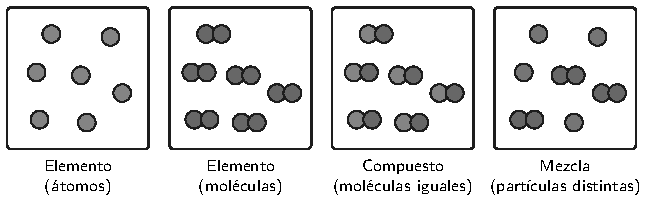
\includegraphics[max width=0.92\linewidth,max height=8.5cm]{qui/atomo_particulas}
\end{center}
\subsection{Elementos y compuestos}
Un \textbf{elemento} no se puede descomponer en sustancias más simples, ni siquiera con una reacción química. Hay cerca de 118, todos en la tabla periódica. Algunos están como átomos sueltos (He, Ne, Fe) y otros como moléculas de átomos iguales (O\textsubscript{2}, N\textsubscript{2}, Cl\textsubscript{2}, O\textsubscript{3}).

 

Un \textbf{compuesto} sí se puede descomponer, pero solo con una \textbf{reacción química}. Por ejemplo, al pasar corriente eléctrica por agua (electrólisis) se obtienen dos gases: hidrógeno y oxígeno.

 

Dos ideas importantes de los compuestos:

 
\begin{itemize}
  \item \textbf{Proporción fija:} el agua siempre tiene 1 g de hidrógeno por cada 8 g de oxígeno, venga de un río o de un glaciar.
  \item \textbf{Propiedades nuevas:} el sodio es un metal que reacciona violentamente con el agua y el cloro es un gas verde y tóxico; juntos forman la sal de mesa, NaCl, que comemos todos los días.
\end{itemize}
  
\begin{ejemplo}[{Ejemplo resuelto}] Clasifica: oro, aire, agua destilada, bronce, CO\textsubscript{2} y ozono (O\textsubscript{3}).\par · Oro (Au): un tipo de átomo \ensuremath{\rightarrow} \textbf{elemento}.\par · Ozono (O\textsubscript{3}): tres átomos, pero todos de oxígeno \ensuremath{\rightarrow} \textbf{elemento}.\par · Agua destilada (H\textsubscript{2}O) y CO\textsubscript{2}: dos elementos unidos \ensuremath{\rightarrow} \textbf{compuestos}.\par · Aire (N\textsubscript{2}, O\textsubscript{2}, Ar, CO\textsubscript{2}\dots{}) y bronce (cobre con estaño): varias sustancias, uniformes \ensuremath{\rightarrow} \textbf{mezclas homogéneas}.\end{ejemplo}
 
\begin{ojo}[{Error típico}] «El O\textsubscript{2} es un compuesto porque tiene dos átomos». No: para ser compuesto debe tener átomos de \textbf{elementos distintos}. Y el agua de la llave no es sustancia pura: lleva sales disueltas. La sustancia pura es el agua destilada.\end{ojo}
\subsection{Mezclas homogéneas y heterogéneas}
Una \textbf{fase} es una parte de la mezcla con el mismo aspecto y las mismas propiedades en todos sus puntos.

 
\begin{itemize}
  \item \textbf{Mezcla homogénea} (o solución): una sola fase. No distingues sus componentes ni con lupa: agua con azúcar, aire, vinagre, acero, bronce.
  \item \textbf{Mezcla heterogénea}: dos o más fases. Agua con aceite, arena con agua, granito, ensalada. La leche y la niebla (coloides) también se clasifican como heterogéneas: al microscopio se ven gotitas o partículas separadas.
\end{itemize}
 

\textbf{¿Por qué el agua y el aceite no se mezclan?} Por la regla «\textbf{lo semejante disuelve a lo semejante}»: las sustancias \textbf{polares} (agua, etanol, acetona) se mezclan entre sí y disuelven sales como el NaCl; las \textbf{apolares} (aceite, hexano, bencina) se mezclan entre sí. Un líquido polar con uno apolar forma dos fases: es una mezcla heterogénea.

  
\begin{clave}[{Esquema para clasificar}] 1. ¿Es uniforme en todos sus puntos? \textbf{No} \ensuremath{\rightarrow} mezcla heterogénea.\par 2. Si es uniforme: ¿se separa por procesos físicos (evaporar, destilar)? \textbf{Sí} \ensuremath{\rightarrow} mezcla homogénea.\par 3. Si no se separa por procesos físicos: ¿se descompone por procesos químicos? \textbf{Sí} \ensuremath{\rightarrow} compuesto. \textbf{No} \ensuremath{\rightarrow} elemento.\end{clave}
 
\begin{ejemplo}[{Ejemplo resuelto}] Al agregar sal a dos líquidos, se disuelve en el líquido T y queda en el fondo del líquido M. Entonces T se comporta como polar y M como apolar. Si se mezclan T y M, se formarán \textbf{dos fases}: una mezcla heterogénea.\end{ejemplo}
 
\begin{ojo}[{Ojo}] «Transparente» no significa «sustancia pura». El agua con sal es transparente y es una mezcla homogénea.\end{ojo}
\subsection{Separar mezclas: filtración y tamizado}
Como en una mezcla cada sustancia conserva sus propiedades, se separan aprovechando una \textbf{diferencia en alguna propiedad física}: tamaño de partícula, densidad, temperatura de ebullición o solubilidad.

 

\textbf{Filtración.} Separa un \textbf{sólido que no está disuelto} de un líquido. La mezcla pasa por un papel filtro: el sólido queda arriba (\textbf{residuo}) y el líquido pasa (\textbf{filtrado}). Se basa en el tamaño de las partículas. Ejemplos: colar el café, los filtros de agua, la mascarilla.

 

\textbf{Tamizado.} Separa \textbf{sólidos de distinto tamaño} con una malla o tamiz: los granos chicos pasan y los grandes quedan. Ejemplos: cernir harina, separar piedras de la arena en una construcción, clasificar mineral en la minería.

  
\begin{center}
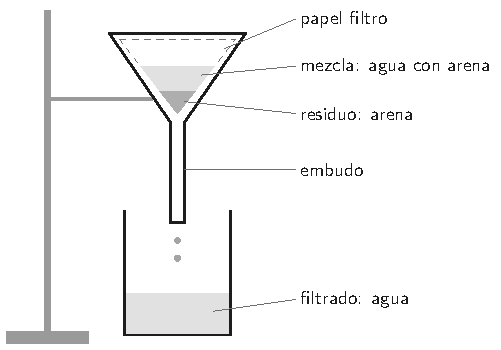
\includegraphics[max width=0.92\linewidth,max height=8.5cm]{qui/atomo_filtracion}
\end{center}
 
\begin{ojo}[{Error típico}] «Filtrando agua de mar obtengo agua sin sal». No: la sal está \textbf{disuelta}, sus partículas son tan pequeñas como las del agua y atraviesan el papel. Lo disuelto no se filtra.\end{ojo}
\subsection{Decantación}
La \textbf{decantación} separa componentes de \textbf{distinta densidad} que no se mezclan.

 

\textbf{Dos líquidos inmiscibles} (agua y aceite): se usa un \textbf{embudo de decantación}. Se deja reposar; el líquido más denso queda abajo. Se abre la llave, sale el líquido de abajo y se cierra justo cuando llega la línea que separa las fases.

 

\textbf{Sólido y líquido} (barro en agua): se deja reposar hasta que el sólido se va al fondo (sedimenta) y se vacía con cuidado el líquido de arriba.

 

\textbf{Aplicación: agua potable.} En las plantas de tratamiento se agregan \textbf{floculantes}, que juntan las partículas pequeñas en grumos (flóculos) más densos que el agua. Los flóculos se van al fondo (\textbf{decantación}) y lo que queda en suspensión se retiene con filtros de arena (\textbf{filtración}).

  
\begin{center}
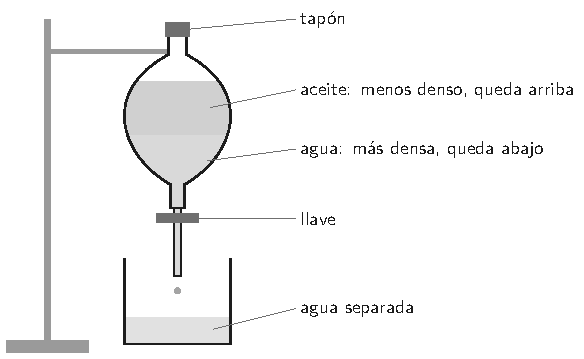
\includegraphics[max width=0.92\linewidth,max height=8.5cm]{qui/atomo_decantacion}
\end{center}
 
\begin{clave}[{Pariente cercano: la centrifugación}] Hace girar la mezcla muy rápido para que lo más denso se vaya al fondo en minutos. Así se separan el plasma y las células de la sangre.\end{clave}
\subsection{Destilación y evaporación}
\textbf{Destilación.} Separa un líquido de lo que tiene disuelto, o dos líquidos \textbf{miscibles} con distinta \textbf{temperatura de ebullición}. Se calienta la mezcla; el componente más volátil (menor temperatura de ebullición) se evapora primero, el vapor se enfría en el \textbf{refrigerante} y se recoge como líquido: el \textbf{destilado}.

 

La \textbf{destilación fraccionada} usa una columna para separar varios líquidos de temperaturas de ebullición cercanas. Así se separa el petróleo en gas, bencina, kerosene y diésel, y así se obtiene el pisco a partir del vino.

 

\textbf{Evaporación.} Si solo interesa el sólido disuelto, se evapora el líquido y el sólido queda. Así se obtiene la sal en las salinas de la costa y el litio en el Salar de Atacama.

  
\begin{clave}[{Mezclas de tres componentes}] Se separan por pasos, cada uno con su propiedad.\par · Arena + sal disuelta en agua: \textbf{filtrar} (queda la arena) y luego \textbf{evaporar} el filtrado (queda la sal).\par · Dos líquidos miscibles + un sólido insoluble: \textbf{filtrar} el sólido y luego \textbf{destilar} los líquidos.\end{clave}
  
\begin{center}
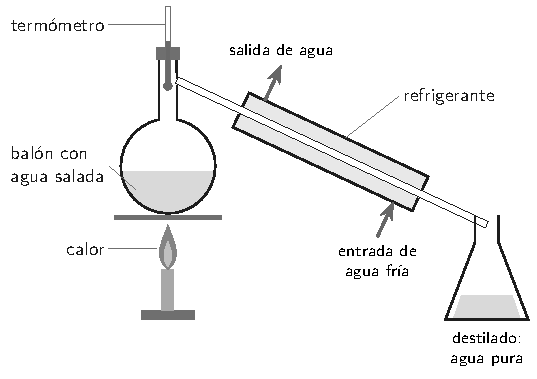
\includegraphics[max width=0.92\linewidth,max height=8.5cm]{qui/atomo_destilacion}
\end{center}
\subsection{Lo clave del tema}
\begin{center}\small
\begin{tabularx}{\linewidth}{@{}>{\raggedright\arraybackslash\hsize=0.51\hsize}X>{\raggedright\arraybackslash\hsize=1.45\hsize}X>{\raggedright\arraybackslash\hsize=0.91\hsize}X>{\raggedright\arraybackslash\hsize=1.13\hsize}X@{}}
\toprule
\textbf{Método} & \textbf{Qué separa} & \textbf{Propiedad que aprovecha} & \textbf{Ejemplo} \\
\midrule
Filtración & sólido no disuelto de un líquido & tamaño de partícula & arena del agua, café \\
Tamizado & sólidos de distinto tamaño & tamaño de partícula & piedras de la arena, harina \\
Decantación & líquidos inmiscibles, o sólido que sedimenta & densidad & agua y aceite, floculantes \\
Destilación & líquidos miscibles, o líquido de su soluto & temperatura de ebullición & petróleo, pisco, agua destilada \\
Evaporación & sólido disuelto de su solvente & volatilidad del solvente & sal de mar, litio \\
\bottomrule
\end{tabularx}
\end{center}
 
\begin{clave}[{Recuerda}] · O\textsubscript{2} es un elemento: todos sus átomos son iguales.\par · Un compuesto tiene partículas iguales formadas por átomos distintos; si hay dos tipos de partículas, es mezcla.\par · El agua con sal es transparente y es una mezcla homogénea.\par · La sal disuelta se separa evaporando o destilando.\par · Dos líquidos miscibles (una sola fase) se separan por destilación.\end{clave}
 
\begin{clave}[{Método PAES}] 1. Cuenta los tipos de partículas o de sustancias: uno \ensuremath{\rightarrow} sustancia pura; varios \ensuremath{\rightarrow} mezcla. 2. Pregunta si es uniforme (homogénea o heterogénea). 3. Para separar, identifica en qué se diferencian los componentes (tamaño, densidad, temperatura de ebullición) y elige el método que usa esa diferencia. 4. Si hay tres componentes, ordena los pasos: primero lo que no está disuelto, al final lo disuelto.\end{clave}
\begin{elejemplo}{PAES Invierno 2027, adaptada}
Un grupo de estudiantes recibe en el laboratorio una muestra de un material desconocido. Para clasificarlo, siguen una secuencia de preguntas y anotan las respuestas en el siguiente esquema:
\begin{center}
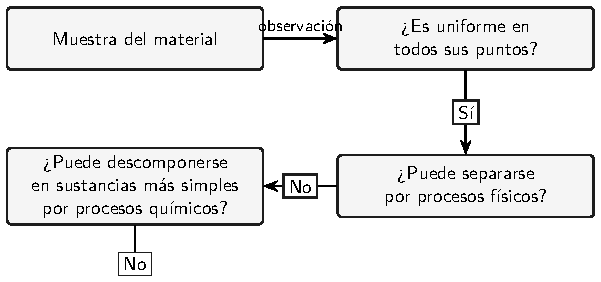
\includegraphics[max width=0.92\linewidth,max height=8.5cm]{qui/atomo_esquema}
\end{center}
\alts{A un elemento.}{A un compuesto.}{A una mezcla homogénea.}{A una mezcla heterogénea.}
\solucion{\textbf{Paso 1. ¿Qué nos piden?} Clasificar el material siguiendo las respuestas del esquema, una por una.

\textbf{Paso 2. ¿Es uniforme? Sí.} Tiene una sola fase. Queda descartada la mezcla heterogénea. Todavía puede ser mezcla homogénea, compuesto o elemento.

\textbf{Paso 3. ¿Se separa por procesos físicos? No.} Una mezcla homogénea, como el agua con sal, sí se separa por procesos físicos (evaporando el agua queda la sal). Como este material no se separa, no es mezcla: es una \textbf{sustancia pura}.

\textbf{Paso 4. ¿Se descompone por procesos químicos? No.} Un compuesto, como el agua, sí se descompone por una reacción química (la electrólisis la separa en hidrógeno y oxígeno). Como este material no se descompone en sustancias más simples, está formado por un solo tipo de átomo.

\textbf{Respuesta:} es un elemento.

\textbf{Comprobación:} un trozo de cobre cumple las tres respuestas: es uniforme, no se separa por filtración, destilación ni evaporación, y ninguna reacción lo convierte en sustancias más simples.

\textbf{¿Por qué no las otras?} «Compuesto» habría tenido «Sí» en la última pregunta: los compuestos se descomponen por procesos químicos. «Mezcla homogénea» habría tenido «Sí» en la segunda pregunta: las mezclas se separan por procesos físicos. «Mezcla heterogénea» habría tenido «No» en la primera: no es uniforme.

\textbf{\color{cienciaD}Para recordar.} Uniforme y sin separarse por métodos físicos es sustancia pura; si además no se descompone químicamente, es un elemento.}{A}
\end{elejemplo}

%% =====================================================================
%% qui_propiedades
\section[Propiedades físicas: densidad, fusión y ebullición]{Propiedades físicas: densidad, fusión y ebullición}
\modcomun\ \ {\color{gris}\itshape Masa, volumen y densidad (d = m/V), propiedades intensivas y extensivas, flotación y desplazamiento de agua; temperaturas de fusión y ebullición, estado físico de una sustancia y curvas de calentamiento de sustancias puras y mezclas.\par}
\subsection{Propiedades extensivas e intensivas}
Una \textbf{propiedad física} se puede medir sin cambiar la identidad de la sustancia: masa, volumen, densidad, temperatura de fusión, temperatura de ebullición, color.

 
\begin{itemize}
  \item \textbf{Extensivas:} dependen de \textbf{cuánta} materia hay. La \textbf{masa} (g, kg) y el \textbf{volumen} (mL, L, cm\textsuperscript{3}) son extensivas: un balde de agua tiene más masa y más volumen que un vaso.
  \item \textbf{Intensivas:} no dependen de la cantidad. La \textbf{densidad}, la \textbf{temperatura de fusión} y la \textbf{temperatura de ebullición} son intensivas: el agua de un vaso y la de un balde hierven a 100 °C a nivel del mar.
\end{itemize}
 

Las intensivas sirven para \textbf{identificar} una sustancia, porque son características de ella. Las extensivas no: 50 g puede ser de agua, de oro o de aire.

  
\begin{ejemplo}[{Ejemplo resuelto}] Un trozo de aluminio tiene 54 g y 20 cm\textsuperscript{3}. Se parte por la mitad. Cada mitad tiene 27 g y 10 cm\textsuperscript{3} (las extensivas se reducen a la mitad), pero la densidad sigue siendo $\dfrac{27}{10} = 2{,}7$ g/cm\textsuperscript{3} y la temperatura de fusión sigue siendo 660 °C (las intensivas no cambian).\end{ejemplo}
 
\begin{ojo}[{Cambio físico o químico}] En un cambio físico la sustancia sigue siendo la misma: el vapor que empaña un espejo sigue siendo agua. En un cambio químico se forma una sustancia nueva: el hierro que se oxida, la manzana que se pone café, el bicarbonato que burbujea con limón.\end{ojo}
\subsection{Densidad: d = m/V}
La \textbf{densidad} dice cuánta masa hay en cada unidad de volumen:

 \[ d = \dfrac{m}{V} \] 

Se mide en g/mL o g/cm\textsuperscript{3} (son lo mismo, porque 1 mL = 1 cm\textsuperscript{3}). El agua líquida tiene $d = 1$ g/mL: cada mililitro de agua tiene 1 g.

 

De la misma fórmula salen las otras dos:

 \[ m = d\cdot V \qquad\qquad V = \dfrac{m}{d} \] 

\textbf{Ejemplo 1.} Un bloque de plomo ($d = 11{,}3$ g/cm\textsuperscript{3}) tiene un volumen de 2,0 cm\textsuperscript{3}. Su masa es $m = 11{,}3\cdot 2{,}0 = 22{,}6$ g.

 

\textbf{Ejemplo 2.} ¿Qué volumen ocupan 46 g de etanol ($d = 0{,}8$ g/mL)? $V = \dfrac{46}{0{,}8} = 57{,}5$ mL.

  
\begin{center}\small
\begin{tabular}{@{}ll@{}}
\toprule
\textbf{Sustancia} & \textbf{Densidad (g/cm\textsuperscript{3})} \\
\midrule
aceite de cocina & 0,92 \\
hielo & 0,92 \\
agua líquida & 1,00 \\
aluminio & 2,7 \\
hierro & 7,9 \\
cobre & 8,96 \\
plomo & 11,3 \\
mercurio & 13,6 \\
oro & 19,3 \\
\bottomrule
\end{tabular}
\end{center}
 
\begin{ojo}[{Error típico}] Sumar o dividir al revés. Revisa las unidades: g/cm\textsuperscript{3} por cm\textsuperscript{3} da g (masa); g dividido por g/cm\textsuperscript{3} da cm\textsuperscript{3} (volumen). Si la unidad no calza, la operación está mal.\end{ojo}
\subsection{Medir el volumen: probeta y desplazamiento de agua}
La masa se mide con una \textbf{balanza}. El volumen de un líquido se mide con una \textbf{probeta}: se lee la marca que coincide con la parte baja de la curva del líquido (el menisco), con los ojos a la altura del líquido.

 

Un sólido de forma irregular, como una piedra, no se puede medir con regla. Se usa el \textbf{desplazamiento de agua}: al sumergirlo, el nivel sube exactamente lo que ocupa el sólido.

 

\textbf{Ejemplo resuelto.} Una piedra de 24 g se sumerge en una probeta con 20 mL de agua y el nivel sube a 28 mL.

 

\textbf{Paso 1.} Volumen de la piedra: $28 - 20 = 8$ mL $= 8$ cm\textsuperscript{3}.

 

\textbf{Paso 2.} Densidad: $d = \dfrac{24}{8} = 3$ g/cm\textsuperscript{3}.

  
\begin{center}
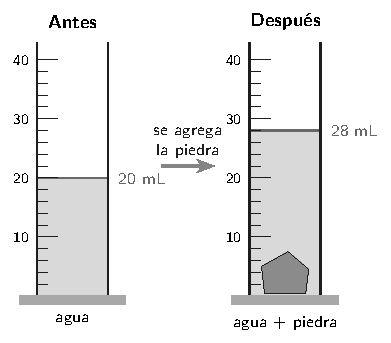
\includegraphics[max width=0.92\linewidth,max height=8.5cm]{qui/atomo_probeta}
\end{center}
 
\begin{ojo}[{Error típico}] Dividir por el volumen final (28 mL) o por el inicial (20 mL). El volumen del sólido es la \textbf{diferencia} entre las dos lecturas.\end{ojo}
 
\begin{clave}[{Precisión}] La probeta mide el volumen con menos precisión que la balanza mide la masa. Con volúmenes pequeños (1 o 2 mL), un error de lectura de 0,1 mL cambia mucho la densidad calculada.\end{clave}
\subsection{Flotación y gráficos de masa y volumen}
\textbf{Flotación.} Un objeto flota en un líquido si su densidad es \textbf{menor} que la del líquido, y se hunde si es mayor. Por eso el hielo (0,92 g/cm\textsuperscript{3}) flota en el agua y una moneda de cobre se hunde. Un huevo se hunde en agua, pero flota en agua con mucha sal: la sal disuelta aumenta la densidad del líquido.

 

Si se juntan líquidos que no se mezclan, se ordenan en capas: el más denso abajo y el menos denso arriba.

 

\textbf{Gráfico de masa versus volumen.} Para una sustancia, la masa es proporcional al volumen: el gráfico es una recta que pasa por el origen, y su \textbf{pendiente es la densidad}. Para leerla, elige un punto de la recta y divide masa por volumen. Mientras más inclinada la recta, mayor la densidad.

  
\begin{center}
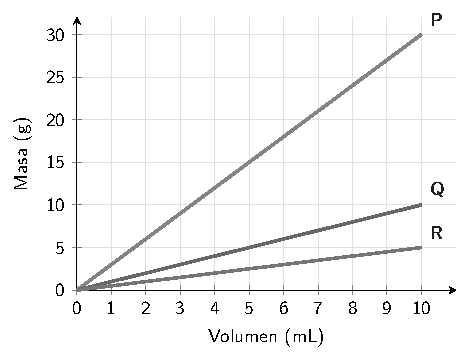
\includegraphics[max width=0.92\linewidth,max height=8.5cm]{qui/atomo_mv_1}
\end{center}
 
\begin{ejemplo}[{Ejemplo resuelto}] En el gráfico, P pasa por (10 mL, 30 g): $d = \dfrac{30}{10} = 3$ g/mL. Q pasa por (10 mL, 10 g): $d = 1$ g/mL, como el agua. R pasa por (10 mL, 5 g): $d = 0{,}5$ g/mL, así que R flota en agua y P se hunde.\end{ejemplo}
 
\begin{ojo}[{Ojo}] La densidad cambia con la temperatura: casi todas las sustancias se dilatan al calentarse, así que su densidad baja un poco. Por eso las tablas indican a qué temperatura se midió.\end{ojo}
\subsection{Temperaturas de fusión y ebullición}
\textbf{Temperatura de fusión:} a la que un sólido pasa a líquido (es la misma a la que el líquido se solidifica). Agua: 0 °C.

 

\textbf{Temperatura de ebullición:} a la que un líquido hierve y pasa a gas (es la misma a la que el gas se condensa). Agua: 100 °C a 1 atm. Depende de la presión: en la cordillera, con menos presión, el agua hierve a menos de 100 °C.

 

\textbf{¿En qué estado está una sustancia a una temperatura T?} Compara T con sus dos temperaturas:

 
\begin{itemize}
  \item T menor que la de fusión \ensuremath{\rightarrow} \textbf{sólido}.
  \item T entre la de fusión y la de ebullición \ensuremath{\rightarrow} \textbf{líquido}.
  \item T mayor que la de ebullición \ensuremath{\rightarrow} \textbf{gas}.
\end{itemize}
  
\begin{ejemplo}[{Ejemplo resuelto}] A 25 °C y 1 atm:
\begin{center}\small
\begin{tabular}{@{}llll@{}}
\toprule
\textbf{Elemento} & \textbf{Fusión (°C)} & \textbf{Ebullición (°C)} & \textbf{Estado} \\
\midrule
Cloro & \ensuremath{-}101 & \ensuremath{-}35 & gas (25 > \ensuremath{-}35) \\
Bromo & \ensuremath{-}7 & 59 & líquido (\ensuremath{-}7 < 25 < 59) \\
Yodo & 114 & 184 & sólido (25 < 114) \\
\bottomrule
\end{tabular}
\end{center}\end{ejemplo}
 
\begin{ojo}[{Error típico con negativos}] \ensuremath{-}35 °C es una temperatura \textbf{más baja} que 25 °C. Si la temperatura de ebullición es negativa, a temperatura ambiente la sustancia ya hirvió: es un gas.\end{ojo}
\subsection{Curvas de calentamiento}
Si se calienta una sustancia y se anota la temperatura cada minuto, se obtiene una \textbf{curva de calentamiento}.

 
\begin{itemize}
  \item En los tramos inclinados, la sustancia está en un solo estado y su temperatura sube.
  \item En los tramos horizontales (\textbf{mesetas}) ocurre un cambio de estado: la sustancia sigue recibiendo calor, pero esa energía se usa en separar las partículas y la temperatura no sube. La primera meseta es la \textbf{fusión} (sólido y líquido juntos) y la segunda, la \textbf{ebullición} (líquido y gas juntos).
\end{itemize}
 

\textbf{Sustancia pura o mezcla.} Una sustancia pura tiene mesetas planas: funde y hierve a una temperatura fija. Una mezcla funde y hierve en un \textbf{rango} de temperaturas: la «meseta» queda inclinada, porque la composición del líquido va cambiando mientras hierve.

  
\begin{center}
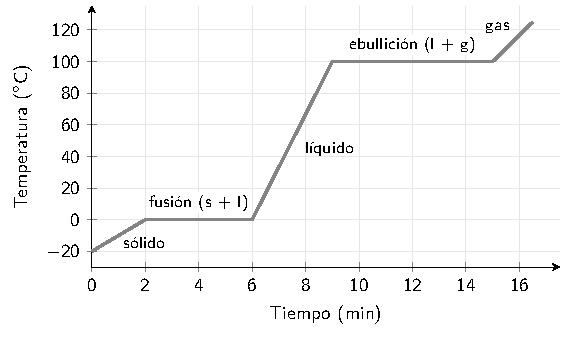
\includegraphics[max width=0.92\linewidth,max height=8.5cm]{qui/atomo_calentamiento}
\end{center}
 
\begin{center}
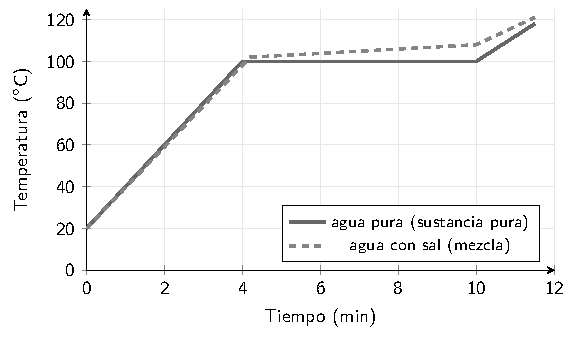
\includegraphics[max width=0.92\linewidth,max height=8.5cm]{qui/atomo_pura_mezcla}
\end{center}
\subsection{Lo clave del tema}
\begin{center}\small
\begin{tabularx}{\linewidth}{@{}>{\raggedright\arraybackslash\hsize=0.97\hsize}X>{\raggedright\arraybackslash\hsize=0.47\hsize}X>{\raggedright\arraybackslash\hsize=1.56\hsize}X@{}}
\toprule
\textbf{Propiedad} & \textbf{Tipo} & \textbf{Cómo se mide o calcula} \\
\midrule
Masa & extensiva & balanza (g) \\
Volumen & extensiva & probeta; sólidos irregulares, desplazamiento de agua (mL = cm\textsuperscript{3}) \\
Densidad & intensiva & $d = \dfrac{m}{V}$; pendiente del gráfico masa-volumen \\
Temperatura de fusión & intensiva & primera meseta de la curva de calentamiento \\
Temperatura de ebullición & intensiva & segunda meseta; depende de la presión \\
\bottomrule
\end{tabularx}
\end{center}
 
\begin{clave}[{Recuerda}] · La densidad es intensiva: si partes un objeto, no cambia.\par · $m = d\cdot V$ (revisa las unidades).\par · Volumen de la piedra = lectura final \ensuremath{-} lectura inicial.\par · En la meseta el calor que entra se usa en el cambio de estado.\par · Si una sustancia hierve a \ensuremath{-}35 °C, a 25 °C ya es gas.\end{clave}
 
\begin{clave}[{Método PAES}] 1. Anota los datos con sus unidades. 2. Elige la fórmula: $d = \dfrac{m}{V}$, $m = d\cdot V$ o $V = \dfrac{m}{d}$. 3. Revisa que las unidades den lo pedido. 4. Para el estado físico, ubica la temperatura entre la de fusión y la de ebullición. 5. En gráficos, lee primero los ejes y sus unidades; en tablas de datos, busca qué variable cambia junto con cuál.\end{clave}
\begin{elejemplo}{PAES Invierno 2027, adaptada}
Como parte de un proyecto escolar, un grupo de estudiantes midió la masa y el volumen de cinco muestras de cobre refinado, que la empresa minera etiqueta con una pureza de 99,99 \%. Con esos valores calcularon la densidad de cada muestra y la compararon con el valor de referencia del cobre, 8,96 g/cm\textsuperscript{3}. Todas las mediciones se hicieron con la misma balanza y la misma probeta, en una sala a temperatura constante:

La profesora les comenta que el trabajo tiene un problema de confiabilidad. ¿Cuál de los siguientes factores lo perjudicó?
\begin{center}\small
\begin{tabularx}{\linewidth}{@{}>{\raggedright\arraybackslash\hsize=0.57\hsize}X>{\raggedright\arraybackslash\hsize=0.51\hsize}X>{\raggedright\arraybackslash\hsize=1.37\hsize}X>{\raggedright\arraybackslash\hsize=1.54\hsize}X@{}}
\toprule
\textbf{Muestra} & \textbf{Masa (g)} & \textbf{Volumen (cm\textsuperscript{3})} & \textbf{Densidad (g/cm\textsuperscript{3})} \\
\midrule
\textbf{1} & 17,204 & 2,0 & 8,6 \\
\textbf{2} & 9,398 & 1,0 & 9,4 \\
\textbf{3} & 13,653 & 1,5 & 9,1 \\
\textbf{4} & 16,998 & 2,0 & 8,5 \\
\textbf{5} & 8,803 & 1,0 & 8,8 \\
\bottomrule
\end{tabularx}
\end{center}
\altslargas{La cantidad de muestras utilizadas.}{Los valores de volumen registrados.}{El uso de un valor de densidad de referencia.}{La procedencia de las muestras desde una empresa.}
\solucion{\textbf{Paso 1. ¿Qué nos piden?} Encontrar qué parte del trabajo hace que los resultados no sean confiables. Primero vemos si los datos tienen sentido.

\textbf{Paso 2. Revisa los cálculos.} $\dfrac{17{,}204}{2{,}0} = 8{,}6$; $\dfrac{9{,}398}{1{,}0} = 9{,}4$; $\dfrac{13{,}653}{1{,}5} = 9{,}1$; $\dfrac{16{,}998}{2{,}0} = 8{,}5$; $\dfrac{8{,}803}{1{,}0} = 8{,}8$. Las cuentas están bien hechas.

\textbf{Paso 3. ¿Qué esperábamos?} Las cinco muestras son del mismo cobre, casi puro. La densidad es intensiva: todas deberían dar casi lo mismo, cerca de 8,96 g/cm\textsuperscript{3}. Pero los resultados van de 8,5 a 9,4: varían demasiado.

\textbf{Paso 4. Busca la causa.} Las masas tienen tres decimales: la balanza es muy precisa. Los volúmenes tienen un solo decimal y son muy pequeños (1 o 2 cm\textsuperscript{3}), medidos con una probeta. Un error de lectura de solo 0,1 cm\textsuperscript{3} en 1,0 cm\textsuperscript{3} es un error del 10 \% en la densidad. Por ejemplo, la muestra 2 daría $\dfrac{9{,}398}{1{,}05} \approx 8{,}95$ g/cm\textsuperscript{3} si su volumen real fuera 1,05 cm\textsuperscript{3}, en vez de 1,0.

\textbf{Respuesta:} los valores de volumen registrados.

\textbf{Comprobación:} si el problema fuera la pureza, todas las densidades se correrían hacia el mismo lado; aquí unas quedan sobre 8,96 y otras bajo 8,96, que es lo típico de un error de medición al azar.

\textbf{¿Por qué no las otras?} Cinco muestras es una cantidad razonable; más muestras no arreglan una medición imprecisa. Comparar con un valor de referencia es justamente lo que permite detectar el problema. Que las muestras vengan de una empresa no afecta la medición: el cobre está etiquetado con 99,99 \% de pureza.

\textbf{\color{cienciaD}Para recordar.} Si una muestra pura da densidades muy distintas, revisa la precisión de las mediciones, sobre todo de los volúmenes pequeños.}{B}
\end{elejemplo}

%% =====================================================================
%% qui_modelos
\section[Modelos atómicos: de Dalton a Bohr]{Modelos atómicos: de Dalton a Bohr}
\modcomun\ \ {\color{gris}\itshape La teoría de Dalton y los modelos de Thomson, Rutherford y Bohr: qué propuso cada uno, qué experimento u observación lo motivó, qué explicó, cuáles fueron sus limitaciones y en qué orden aparecieron.\par}
\subsection{Por qué hay varios modelos atómicos}
Nadie ha visto un átomo a simple vista. Un \textbf{modelo atómico} es una representación que explica lo que se observa en los experimentos. Cuando aparece una observación que el modelo no puede explicar, se propone uno nuevo que sí la explique.

 

Así, cada modelo corrige al anterior:

 
\begin{center}\small
\begin{tabularx}{\linewidth}{@{}>{\raggedright\arraybackslash\hsize=0.72\hsize}X>{\raggedright\arraybackslash\hsize=0.81\hsize}X>{\raggedright\arraybackslash\hsize=1.48\hsize}X@{}}
\toprule
\textbf{Año} & \textbf{Modelo} & \textbf{Idea central} \\
\midrule
1808 & Dalton & átomos indivisibles \\
1897--1904 & Thomson & el átomo tiene electrones \\
1911 & Rutherford & núcleo pequeño, positivo y denso \\
1913 & Bohr & niveles de energía \\
1926 en adelante & mecano-cuántico & orbitales (zonas de probabilidad) \\
\bottomrule
\end{tabularx}
\end{center}
  
\gatotip[\gatogris]{\textbf{Para recordar el orden.} Cada modelo agrega algo «más adentro» del átomo: Dalton (el átomo entero) \ensuremath{\rightarrow} Thomson (sus electrones) \ensuremath{\rightarrow} Rutherford (su núcleo) \ensuremath{\rightarrow} Bohr (la energía de los electrones).}
  
\begin{center}
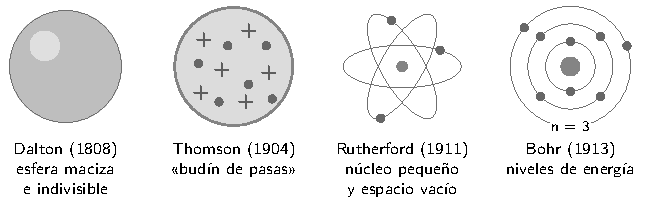
\includegraphics[max width=0.92\linewidth,max height=8.5cm]{qui/atomo_modelos}
\end{center}
\subsection{Dalton: el átomo indivisible}
John Dalton (1808) propuso la primera teoría atómica con base experimental. Sus postulados:

 
\begin{itemize}
  \item La materia está formada por partículas muy pequeñas e \textbf{indivisibles}: los átomos.
  \item Los átomos de un mismo elemento son \textbf{iguales} entre sí (misma masa y propiedades) y distintos de los de otros elementos.
  \item Los compuestos se forman al combinarse átomos de distintos elementos en \textbf{proporciones de números enteros sencillos}.
  \item En una reacción química los átomos \textbf{se reordenan}: no se crean ni se destruyen.
\end{itemize}
 

Con esto explicó la ley de conservación de la masa y la ley de las proporciones definidas.

  
\begin{ojo}[{Limitaciones}] El átomo \textbf{sí es divisible}: tiene electrones, protones y neutrones. Y no todos los átomos de un elemento tienen la misma masa: existen los \textbf{isótopos}. Su modelo no dice nada sobre cargas eléctricas.\end{ojo}
 
\begin{ejemplo}[{Ejemplo resuelto}] ¿Qué postulado de Dalton explica que en una reacción la masa total no cambie? El último: los átomos solo se reordenan. Si hay los mismos átomos antes y después, la masa es la misma.\end{ejemplo}
\subsection{Thomson: el descubrimiento del electrón}
J. J. Thomson trabajó con \textbf{tubos de rayos catódicos}: tubos de vidrio casi sin aire, con un metal en cada extremo conectado a alto voltaje. Desde el polo negativo salía un rayo que se desviaba hacia una placa con carga \textbf{positiva}.

 

\textbf{Conclusión:} el rayo está formado por partículas con \textbf{carga negativa}, mucho más livianas que un átomo, y aparecen con cualquier metal. Esas partículas, los \textbf{electrones}, forman parte de todos los átomos. Por lo tanto, el átomo \textbf{no es indivisible}.

 

\textbf{Modelo del «budín de pasas»} (1904): el átomo es una esfera con carga positiva repartida de manera uniforme, y los electrones están incrustados en ella, como pasas en un budín. Las cargas positivas y negativas se compensan: el átomo es neutro.

  
\begin{ojo}[{Limitación}] Con la carga positiva repartida por toda la esfera, ninguna partícula debería rebotar al chocar con un átomo. El experimento de Rutherford mostró lo contrario.\end{ojo}
 
\begin{clave}[{Error típico}] «Thomson descubrió el núcleo». No: Thomson descubrió el \textbf{electrón}. El núcleo lo propuso Rutherford.\end{clave}
\subsection{Rutherford: el experimento de la lámina de oro}
En 1911, el equipo de Ernest Rutherford bombardeó una lámina de oro muy delgada con \textbf{partículas alfa} (partículas con carga positiva) y registró hacia dónde salían en una pantalla.

 
\begin{center}\small
\begin{tabularx}{\linewidth}{@{}>{\raggedright\arraybackslash\hsize=1.00\hsize}X>{\raggedright\arraybackslash\hsize=1.00\hsize}X@{}}
\toprule
\textbf{Observación} & \textbf{Conclusión} \\
\midrule
Casi todas pasan sin desviarse & el átomo es casi todo \textbf{espacio vacío} \\
Algunas se desvían & hay una zona con carga \textbf{positiva} que las repele \\
Muy pocas (1 de cada 10.000 a 100.000) rebotan & esa zona es muy \textbf{pequeña} y muy \textbf{densa}: concentra casi toda la masa \\
\bottomrule
\end{tabularx}
\end{center}
 

\textbf{Modelo nuclear} (o planetario): un \textbf{núcleo} diminuto, positivo, con casi toda la masa del átomo, y los electrones girando alrededor, lejos de él. Si el átomo fuera un estadio, el núcleo sería una bolita en el centro de la cancha.

  
\begin{ojo}[{Limitación}] Según la física de la época, un electrón que gira debería emitir energía, perder velocidad y caer en espiral al núcleo: el átomo no sería estable. Tampoco explicaba por qué cada elemento emite luz solo de ciertos colores.\end{ojo}
  
\begin{center}
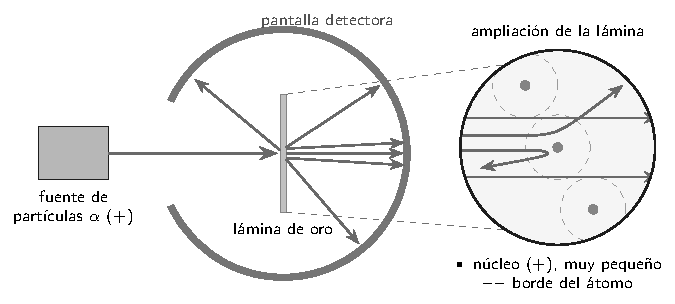
\includegraphics[max width=0.92\linewidth,max height=8.5cm]{qui/atomo_rutherford}
\end{center}
\subsection{Bohr: los niveles de energía}
Niels Bohr (1913) mantuvo el núcleo de Rutherford y agregó reglas para los electrones:

 
\begin{itemize}
  \item Los electrones giran en \textbf{órbitas circulares} de radio y \textbf{energía fijos}, llamadas niveles ($n = 1, 2, 3$\dots{}). Mientras está en su nivel, el electrón no pierde energía.
  \item Mientras más lejos del núcleo, \textbf{mayor es la energía} del nivel y \textbf{menor la energía que se necesita para arrancar} el electrón del átomo.
  \item Un electrón \textbf{absorbe} energía y salta a un nivel más alejado. Al volver a un nivel más cercano, \textbf{emite} esa energía como luz.
\end{itemize}
 

Como los niveles tienen energías fijas, solo se emiten ciertas energías, es decir, ciertos colores: el \textbf{espectro de líneas} de cada elemento. Por eso el sodio da luz amarilla y el cobre, verde, en el ensayo a la llama y en los fuegos artificiales.

  
\begin{clave}[{En los diagramas de la PAES}] Para los primeros 20 elementos, los electrones se ubican así: hasta 2 en el primer nivel, hasta 8 en el segundo y hasta 8 en el tercero.\end{clave}
 
\begin{ojo}[{Limitación}] Funciona muy bien para el hidrógeno, pero no para átomos con muchos electrones. El modelo actual (mecano-cuántico) reemplaza las órbitas por \textbf{orbitales}: zonas donde es más probable encontrar al electrón.\end{ojo}
  
\begin{center}
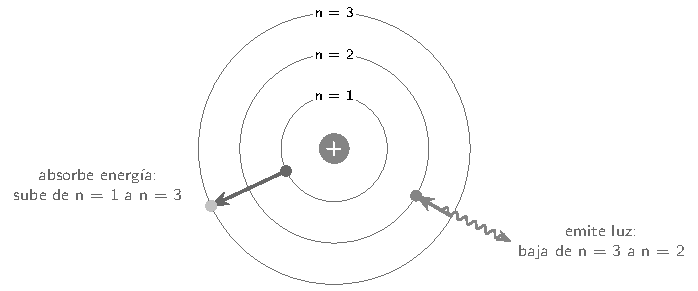
\includegraphics[max width=0.92\linewidth,max height=8.5cm]{qui/atomo_bohr}
\end{center}
\subsection{Lo clave del tema}
\begin{center}\small
\begin{tabularx}{\linewidth}{@{}>{\raggedright\arraybackslash\hsize=0.52\hsize}X>{\raggedright\arraybackslash\hsize=1.04\hsize}X>{\raggedright\arraybackslash\hsize=1.22\hsize}X>{\raggedright\arraybackslash\hsize=1.22\hsize}X@{}}
\toprule
\textbf{Modelo} & \textbf{Evidencia} & \textbf{Qué aporta} & \textbf{Limitación} \\
\midrule
Dalton (1808) & leyes de la masa en las reacciones & átomos indivisibles que se reordenan & el átomo es divisible; hay isótopos \\
Thomson (1904) & rayos catódicos & electrones (\ensuremath{-}) en una esfera positiva & no explica los rebotes de partículas alfa \\
Rutherford (1911) & lámina de oro y partículas alfa & núcleo pequeño, denso y positivo; espacio vacío & el electrón caería al núcleo; no explica los espectros \\
Bohr (1913) & espectros de líneas & niveles de energía fijos; absorción y emisión & solo funciona bien para el hidrógeno \\
\bottomrule
\end{tabularx}
\end{center}
 
\begin{clave}[{Recuerda}] · Thomson descubrió el electrón; Rutherford propuso el núcleo.\par · Casi todas las partículas alfa pasan derecho porque el átomo es casi vacío; unas pocas rebotan al chocar con el núcleo, denso y positivo.\par · Las partículas alfa se desvían por la repulsión del núcleo positivo; los electrones son muy livianos para desviarlas.\par · El electrón absorbe energía al subir de nivel y emite luz al bajar.\par · Los electrones más lejanos son los más fáciles de arrancar.\end{clave}
 
\begin{clave}[{Método PAES}] 1. Identifica de qué modelo habla el texto por su experimento o su idea clave (rayos catódicos \ensuremath{\rightarrow} Thomson; lámina de oro \ensuremath{\rightarrow} Rutherford; niveles y espectros \ensuremath{\rightarrow} Bohr). 2. Une cada observación con la conclusión que permite. 3. Descarta las alternativas que mezclan ideas de modelos distintos o que son ciertas pero no salen de lo descrito.\end{clave}
\begin{elejemplo}{PAES Invierno 2026, adaptada}
A comienzos del siglo XX, un científico propuso un modelo atómico formado por un núcleo y electrones girando a su alrededor. El modelo surgió de un experimento en el que se lanzaron partículas alfa, de carga positiva, contra una lámina muy delgada de oro:

La gran mayoría de las partículas atravesó la lámina sin cambiar su trayectoria. Unas pocas se desviaron y, aproximadamente, una de cada cien mil rebotó en dirección contraria.

De acuerdo con lo anterior, ¿cuál de las siguientes inferencias es correcta?
\begin{center}
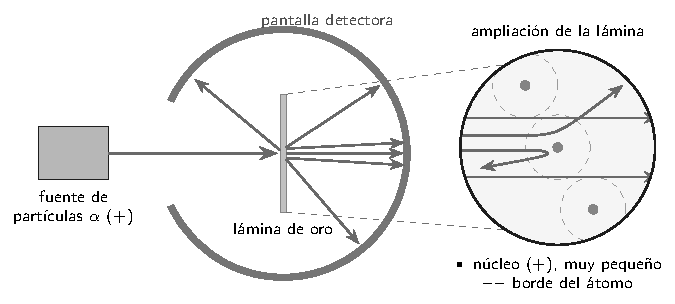
\includegraphics[max width=0.92\linewidth,max height=8.5cm]{qui/atomo_rutherford}
\end{center}
\altslargas{El átomo tiene un núcleo que ocupa casi todo su volumen.}{Los electrones del átomo repelen a las partículas alfa.}{El átomo está formado principalmente por espacio vacío.}{El núcleo del átomo tiene carga negativa.}
\solucion{\textbf{Paso 1. ¿Qué nos piden?} Una inferencia que se apoye en las observaciones del experimento de Rutherford. Unimos cada observación con lo que permite concluir.

\textbf{Paso 2. «La gran mayoría pasa sin desviarse».} Si casi todas las partículas atraviesan los miles de capas de átomos de la lámina sin chocar con nada, dentro del átomo casi no hay nada que se interponga: el átomo es principalmente \textbf{espacio vacío}.

\textbf{Paso 3. «Unas pocas se desvían».} Las partículas alfa son positivas. Si algo las desvía, es una zona con carga \textbf{positiva} que las repele.

\textbf{Paso 4. «Una de cada cien mil rebota».} Para hacer rebotar a una partícula tan rápida, esa zona tiene que ser muy densa. Y como casi nunca se choca con ella, debe ser muy pequeña: es el núcleo.

\textbf{Respuesta:} el átomo está formado principalmente por espacio vacío.

\textbf{Comprobación:} si el núcleo fuera grande, muchas partículas chocarían con él y rebotarían; pero rebota solo 1 de cada 100.000, así que el núcleo ocupa una parte ínfima del volumen.

\textbf{¿Por qué no las otras?} «Un núcleo que ocupa casi todo el volumen» contradice que casi todas las partículas pasen. Los electrones tienen carga negativa: atraerían a las partículas alfa, no las repelerían, y además son tan livianos que no pueden desviarlas. Un núcleo negativo atraería a las partículas alfa; no las haría rebotar.

\textbf{\color{cienciaD}Para recordar.} Pasan derecho \ensuremath{\rightarrow} espacio vacío. Se desvían o rebotan \ensuremath{\rightarrow} núcleo pequeño, denso y positivo.}{C}
\end{elejemplo}

%% =====================================================================
%% qui_particulas
\section[Protones, neutrones y electrones]{Protones, neutrones y electrones}
\modcomun\ \ {\color{gris}\itshape Las partículas del átomo, el número atómico Z y el número másico A, la notación de núclido, los isótopos y los iones (cationes y aniones), y cómo contar protones, neutrones y electrones en símbolos y diagramas.\par}
\subsection{Las tres partículas del átomo}
Todo átomo tiene un \textbf{núcleo} muy pequeño, con protones y neutrones, y alrededor, los \textbf{electrones}.

 
\begin{center}\small
\begin{tabular}{@{}llll@{}}
\toprule
\textbf{Partícula} & \textbf{Carga} & \textbf{Masa relativa} & \textbf{Ubicación} \\
\midrule
Protón (p\textsuperscript{+}) & +1 & 1 u & núcleo \\
Neutrón (n\textsuperscript{0}) & 0 & 1 u & núcleo \\
Electrón (e\textsuperscript{\ensuremath{-}}) & \ensuremath{-}1 & casi 0 (1/1840 u) & niveles, fuera del núcleo \\
\bottomrule
\end{tabular}
\end{center}
 

Dos consecuencias:

 
\begin{itemize}
  \item La \textbf{masa} del átomo está casi toda en el núcleo: protones y neutrones.
  \item La \textbf{carga} depende de protones y electrones. Si hay tantos electrones como protones, las cargas se anulan y el átomo es \textbf{neutro}.
\end{itemize}
  
\begin{center}
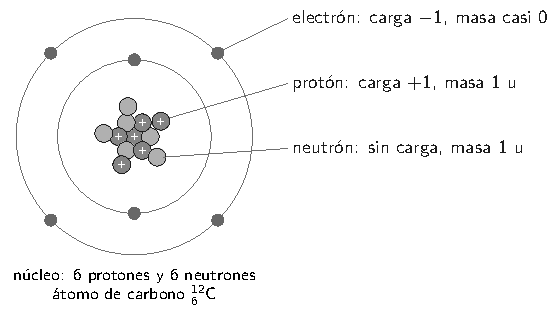
\includegraphics[max width=0.92\linewidth,max height=8.5cm]{qui/atomo_partes}
\end{center}
 
\begin{ojo}[{Ojo}] Los neutrones no tienen carga, pero sí masa: cuentan para la masa del átomo y no cuentan para su carga.\end{ojo}
\subsection{Número atómico Z y número másico A}
\textbf{Número atómico (Z):} la cantidad de \textbf{protones}. Es el «carnet de identidad» del elemento: todos los átomos de carbono tienen 6 protones, y cualquier átomo con 6 protones es carbono. La tabla periódica ordena los elementos según Z.

 

\textbf{Número másico (A):} la cantidad de \textbf{protones más neutrones}, las partículas del núcleo.

 \[ A = Z + n \qquad\Rightarrow\qquad n = A - Z \] 

\textbf{Notación de núclido:} A arriba a la izquierda, Z abajo a la izquierda y la carga, si la hay, arriba a la derecha: $\,{}^{A}_{Z}\text{X}^{\text{carga}}$.

 

En un átomo \textbf{neutro}, electrones = protones = Z.

  
\begin{ejemplo}[{Ejemplo resuelto}] $\,{}^{23}_{11}\text{Na}$.\par \textbf{Paso 1.} Protones: Z = 11.\par \textbf{Paso 2.} Neutrones: $23 - 11 = 12$.\par \textbf{Paso 3.} Electrones: no tiene carga, así que es neutro: 11.\end{ejemplo}
 
\begin{ojo}[{Error típico}] Confundir Z con A, o creer que los neutrones son iguales a los protones. En $\,{}^{35}_{17}\text{Cl}$ hay 17 protones y $35 - 17 = 18$ neutrones.\end{ojo}
 
\begin{clave}[{Masa atómica de la tabla}] No es un número entero (Cl = 35,5) porque es un promedio de los isótopos naturales del elemento. El número másico A, en cambio, siempre es entero.\end{clave}
\subsection{Iones: cationes y aniones}
Un \textbf{ion} es un átomo (o grupo de átomos) con carga eléctrica, porque \textbf{ganó o perdió electrones}. Los protones no cambian: siguen siendo los mismos, y por eso el elemento sigue siendo el mismo.

 
\begin{itemize}
  \item \textbf{Catión} (carga +): \textbf{perdió} electrones. Na\textsuperscript{+}: 11 protones y 10 electrones.
  \item \textbf{Anión} (carga \ensuremath{-}): \textbf{ganó} electrones. Cl\textsuperscript{\ensuremath{-}}: 17 protones y 18 electrones.
\end{itemize}
 

La regla para contar electrones:

 \[ \text{electrones} = Z - \text{carga} \] 

Con carga 2+: $Z - 2$. Con carga 2\ensuremath{-}: $Z - (-2) = Z + 2$.

  
\begin{ejemplo}[{Ejemplo resuelto}] $\,{}^{40}_{20}\text{Ca}^{2+}$.\par \textbf{Paso 1.} Protones: 20.\par \textbf{Paso 2.} Neutrones: $40 - 20 = 20$.\par \textbf{Paso 3.} Electrones: carga 2+, perdió 2: $20 - 2 = 18$.\end{ejemplo}
 
\begin{ejemplo}[{Ejemplo resuelto}] $\,{}^{32}_{16}\text{S}^{2-}$: 16 protones, $32 - 16 = 16$ neutrones y $16 + 2 = 18$ electrones.\end{ejemplo}
 
\begin{ojo}[{Error típico}] «El catión ganó protones». No: un ion nunca cambia sus protones. Si cambiaran los protones, sería otro elemento. Y el signo engaña: carga + significa \textbf{menos} electrones.\end{ojo}
\subsection{Isótopos, isóbaros e isótonos}
\textbf{Isótopos:} átomos del \textbf{mismo elemento} (igual Z) con distinto número de neutrones y, por eso, distinto A. Tienen las mismas propiedades químicas, porque tienen los mismos protones y electrones; solo cambia su masa.

 
\begin{itemize}
  \item Carbono: $\,{}^{12}_{6}\text{C}$ (6 n), $\,{}^{13}_{6}\text{C}$ (7 n) y $\,{}^{14}_{6}\text{C}$ (8 n). El carbono 14 se usa para datar restos arqueológicos.
  \item Hidrógeno: protio $\,{}^{1}_{1}\text{H}$ (0 n), deuterio $\,{}^{2}_{1}\text{H}$ (1 n) y tritio $\,{}^{3}_{1}\text{H}$ (2 n).
\end{itemize}
 

La PAES a veces define otras dos palabras en el enunciado:

 
\begin{itemize}
  \item \textbf{Isóbaros:} igual A, distinto Z (elementos distintos): $\,{}^{40}_{18}\text{Ar}$ y $\,{}^{40}_{20}\text{Ca}$.
  \item \textbf{Isótonos:} igual número de neutrones: $\,{}^{39}_{19}\text{K}$ y $\,{}^{40}_{20}\text{Ca}$ (20 n cada uno).
\end{itemize}
  
\begin{center}\small
\begin{tabular}{@{}llll@{}}
\toprule
\textbf{Comparación} & \textbf{Z (protones)} & \textbf{A} & \textbf{Neutrones} \\
\midrule
Isótopos & igual & distinto & distinto \\
Isóbaros & distinto & igual & distinto \\
Isótonos & distinto & distinto & igual \\
\bottomrule
\end{tabular}
\end{center}
 
\begin{ejemplo}[{Ejemplo resuelto}] ¿En qué se diferencian $\,{}^{28}_{14}\text{Si}$, $\,{}^{29}_{14}\text{Si}$ y $\,{}^{30}_{14}\text{Si}$? Tienen igual Z (14 protones) y, como son neutros, 14 electrones. Se diferencian en los neutrones: 14, 15 y 16. Son isótopos.\end{ejemplo}
\subsection{Contar partículas en un diagrama}
En la PAES aparecen diagramas de Bohr con el núcleo y los electrones dibujados como puntos en sus niveles. Para leerlos:

 

\textbf{Paso 1.} Lee en el núcleo los protones (p) y los neutrones (n).

 

\textbf{Paso 2.} Cuenta los electrones de todos los niveles.

 

\textbf{Paso 3.} Compara: si hay más electrones que protones, es un anión; si hay menos, un catión; si son iguales, un átomo neutro.

 

\textbf{Paso 4.} Arma la notación: Z = protones, A = protones + neutrones, carga = protones \ensuremath{-} electrones.

 

Si el diagrama muestra solo neutrones y dice que el átomo es neutro, los protones son iguales a los electrones que cuentas.

  
\begin{center}
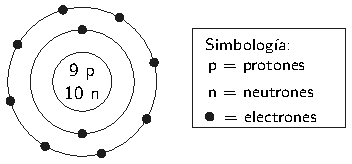
\includegraphics[max width=0.92\linewidth,max height=8.5cm]{qui/atomo_fluoruro}
\end{center}
 
\begin{ejemplo}[{Ejemplo resuelto}] En el diagrama: 9 p y 10 n en el núcleo; electrones: $2 + 8 = 10$. Z = 9, A = 9 + 10 = 19 y carga = 9 \ensuremath{-} 10 = \ensuremath{-}1. Es $\,{}^{19}_{9}\text{X}^{-}$: el ion fluoruro, F\textsuperscript{\ensuremath{-}}.\end{ejemplo}
\subsection{Lo clave del tema}
\begin{center}\small
\begin{tabularx}{\linewidth}{@{}>{\raggedright\arraybackslash\hsize=0.72\hsize}X>{\raggedright\arraybackslash\hsize=0.67\hsize}X>{\raggedright\arraybackslash\hsize=1.61\hsize}X@{}}
\toprule
\textbf{Quiero saber} & \textbf{Cómo lo calculo} & \textbf{Ejemplo: $\,{}^{56}_{26}\text{Fe}^{3+}$} \\
\midrule
Protones & Z & 26 \\
Neutrones & A \ensuremath{-} Z & 56 \ensuremath{-} 26 = 30 \\
Electrones & Z \ensuremath{-} carga & 26 \ensuremath{-} 3 = 23 \\
¿Mismo elemento? & mismo Z & todo átomo con 26 protones es hierro \\
\bottomrule
\end{tabularx}
\end{center}
 
\begin{clave}[{Recuerda}] · Neutrones = A \ensuremath{-} Z.\par · Una carga positiva indica electrones perdidos: Fe\textsuperscript{3+} tiene 26 \ensuremath{-} 3 = 23 electrones.\par · En un ion solo cambian los electrones; los protones definen el elemento.\par · Los isótopos tienen igual Z y distinto número de neutrones.\par · Neutrones y protones pueden ser distintos: $\,{}^{35}_{17}\text{Cl}$ tiene 18 neutrones.\end{clave}
 
\begin{clave}[{Método PAES}] 1. Haz una tablita con p, n y e de cada especie antes de leer las alternativas. 2. Protones = Z; neutrones = A \ensuremath{-} Z; electrones = Z \ensuremath{-} carga. 3. Para comparar especies, resta fila por fila. 4. Para «mismo elemento» o «isótopos», mira solo Z.\end{clave}
\begin{elejemplo}{PAES Invierno 2026, adaptada}
La siguiente tabla presenta el número de protones de cuatro iones:

A partir de la tabla, ¿cuál de las siguientes comparaciones del número de electrones de los iones es correcta?
\begin{center}\small
\begin{tabular}{@{}ll@{}}
\toprule
\textbf{Ion} & \textbf{N.° de protones} \\
\midrule
\textbf{I\textsuperscript{\ensuremath{-}}} & 53 \\
\textbf{S\textsuperscript{2\ensuremath{-}}} & 16 \\
\textbf{Mg\textsuperscript{2+}} & 12 \\
\textbf{Al\textsuperscript{3+}} & 13 \\
\bottomrule
\end{tabular}
\end{center}
\altslargas{El ion S\textsuperscript{2\ensuremath{-}} tiene 4 electrones más que el ion Mg\textsuperscript{2+}.}{El ion Mg\textsuperscript{2+} tiene 1 electrón menos que el ion Al\textsuperscript{3+}.}{El ion I\textsuperscript{\ensuremath{-}} tiene 36 electrones más que el ion S\textsuperscript{2\ensuremath{-}}.}{El ion Al\textsuperscript{3+} tiene 40 electrones menos que el ion I\textsuperscript{\ensuremath{-}}.}
\solucion{\textbf{Paso 1. ¿Qué nos piden?} Comparar electrones, pero la tabla da protones. Primero calculamos los electrones de cada ion con electrones = protones \ensuremath{-} carga.

\textbf{Paso 2. I\textsuperscript{\ensuremath{-}}.} Carga \ensuremath{-}1: ganó 1 electrón. $53 + 1 = 54$ electrones.

\textbf{Paso 3. S\textsuperscript{2\ensuremath{-}}.} Ganó 2: $16 + 2 = 18$ electrones.

\textbf{Paso 4. Mg\textsuperscript{2+}.} Perdió 2: $12 - 2 = 10$ electrones.

\textbf{Paso 5. Al\textsuperscript{3+}.} Perdió 3: $13 - 3 = 10$ electrones.

\textbf{Paso 6. Compara.} I\textsuperscript{\ensuremath{-}} y S\textsuperscript{2\ensuremath{-}}: $54 - 18 = 36$. \ding{52} S\textsuperscript{2\ensuremath{-}} y Mg\textsuperscript{2+}: $18 - 10 = 8$. Mg\textsuperscript{2+} y Al\textsuperscript{3+}: $10 - 10 = 0$, tienen los mismos. Al\textsuperscript{3+} y I\textsuperscript{\ensuremath{-}}: $54 - 10 = 44$.

\textbf{Respuesta:} el ion I\textsuperscript{\ensuremath{-}} tiene 36 electrones más que el ion S\textsuperscript{2\ensuremath{-}}.

\textbf{Comprobación:} I\textsuperscript{\ensuremath{-}} tiene los mismos electrones que el gas noble xenón (54) y S\textsuperscript{2\ensuremath{-}}, los mismos que el argón (18): $54 - 18 = 36$ \ding{52}.

\textbf{¿Por qué no las otras?} Las otras tres comparan \textbf{protones} en vez de electrones, olvidando la carga: $16 - 12 = 4$, $13 - 12 = 1$ y $53 - 13 = 40$. Con los electrones, las diferencias reales son 8, 0 y 44.

\textbf{\color{cienciaD}Para recordar.} Antes de comparar iones, convierte protones en electrones: electrones = Z \ensuremath{-} carga.}{C}
\end{elejemplo}

\chapter{Química orgánica}
%% =====================================================================
%% qui_carbono
\section[El átomo de carbono]{El átomo de carbono}
\modcomun\ \ {\color{gris}\itshape Por qué el carbono forma cuatro enlaces, cómo contar enlaces sigma y pi, cómo reconocer la hibridación sp³, sp² y sp de cada carbono y cómo cambian la energía, la longitud y el ángulo de enlace.\par}
\subsection{Tetravalencia: el carbono siempre forma 4 enlaces}
El carbono tiene $Z = 6$: su configuración es 1s\textsuperscript{2} 2s\textsuperscript{2} 2p\textsuperscript{2}. Tiene \textbf{4 electrones de valencia} y los comparte todos: forma siempre \textbf{4 enlaces covalentes}. A esto se le llama \textbf{tetravalencia}.

 

Los 4 enlaces pueden repartirse de varias formas: cuatro simples, un doble y dos simples, un triple y un simple, o dos dobles. Lo que nunca cambia es la suma: \textbf{4}.

 

Además, el carbono se une fácilmente con otros carbonos (\textbf{concatenación}): forma cadenas largas, ramificadas y anillos. Por eso existen millones de compuestos orgánicos.

 
\begin{center}\small
\begin{tabular}{@{}ll@{}}
\toprule
\textbf{Átomo} & \textbf{N.º de enlaces que forma} \\
\midrule
C & 4 \\
N & 3 \\
O, S & 2 \\
H, F, Cl, Br, I & 1 \\
\bottomrule
\end{tabular}
\end{center}
  
\begin{ejemplo}[{Ejemplo: revisa una estructura}] En CH\textsubscript{2}=CH--CH\textsubscript{3} (propeno):\par · C1: doble (cuenta 2) + 2 H = 4 \ding{52}\par · C2: doble (2) + 1 H + 1 simple = 4 \ding{52}\par · C3: 1 simple + 3 H = 4 \ding{52}\end{ejemplo}
 
\begin{ojo}[{Error típico}] Contar un enlace doble como 1. Un doble "gasta" 2 de los 4 enlaces del carbono y un triple gasta 3. Por eso el CH de un doble enlace tiene un solo H, y el C de un triple interno no tiene ninguno.\end{ojo}
\subsection{Enlaces simple, doble y triple: sigma y pi}
Cada línea de una fórmula es un par de electrones compartidos. Pero no todos los enlaces son iguales:

 
\begin{itemize}
  \item \textbf{Enlace simple} (C--C, C--H): 1 enlace \textbf{sigma} ($\sigma$).
  \item \textbf{Enlace doble} (C=C, C=O): 1 $\sigma$ + 1 \textbf{pi} ($\pi$).
  \item \textbf{Enlace triple} (C\ensuremath{\equiv}C, C\ensuremath{\equiv}N): 1 $\sigma$ + 2 $\pi$.
\end{itemize}
 

El enlace $\sigma$ une los núcleos de frente; el $\pi$ se forma por los lados, con orbitales p que quedaron sin mezclar. Entre dos átomos hay \textbf{como máximo un} $\sigma$.

 
\begin{clave}[{Método para contar}] 1. Dibuja (o imagina) todos los H. 2. Cada enlace, sea simple, doble o triple, aporta \textbf{exactamente 1} $\sigma$. 3. Los $\pi$ son las líneas extra: 1 por cada doble y 2 por cada triple.\end{clave}
 
\gatotip[\gatonegro]{\textbf{Atajo.} En una molécula sin anillos, n.º de $\sigma$ = n.º de átomos \ensuremath{-} 1. Por cada anillo, suma 1. Benceno C\textsubscript{6}H\textsubscript{6}: $12 - 1 + 1 = 12$ enlaces $\sigma$.}
  
\begin{center}
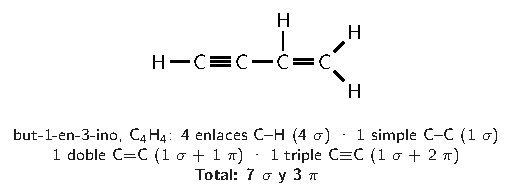
\includegraphics[max width=0.92\linewidth,max height=8.5cm]{qui/org_sigma_pi}
\end{center}
 
\begin{ojo}[{Error típico}] Contar el triple como 3 $\sigma$, o "olvidar" los C--H porque no se dibujan en la fórmula topológica. Los C--H también son enlaces $\sigma$.\end{ojo}
\subsection{Hibridación: sp³, sp² y sp}
Para formar sus enlaces, el carbono "mezcla" su orbital 2s con orbitales 2p y obtiene orbitales nuevos, iguales entre sí: los \textbf{orbitales híbridos}. Cuántos mezcla depende de cuántos enlaces $\pi$ tenga que formar.

 
\begin{center}
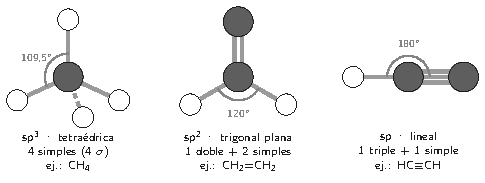
\includegraphics[max width=0.92\linewidth,max height=8.5cm]{qui/org_geometrias}
\end{center}
 
\begin{center}\small
\begin{tabularx}{\linewidth}{@{}>{\raggedright\arraybackslash\hsize=0.76\hsize}X>{\raggedright\arraybackslash\hsize=1.68\hsize}X>{\raggedright\arraybackslash\hsize=0.97\hsize}X>{\raggedright\arraybackslash\hsize=0.76\hsize}X>{\raggedright\arraybackslash\hsize=0.49\hsize}X>{\raggedright\arraybackslash\hsize=1.35\hsize}X@{}}
\toprule
\textbf{Hibridación} & \textbf{Enlaces del C} & \textbf{Átomos unidos al C} & \textbf{Geometría} & \textbf{Ángulo} & \textbf{Ejemplo} \\
\midrule
sp\textsuperscript{3} & 4 simples & 4 & tetraédrica & 109,5° & CH\textsubscript{4}, alcanos, C de un CH\textsubscript{3} \\
sp\textsuperscript{2} & 1 doble + 2 simples & 3 & trigonal plana & 120° & eteno, C=O, benceno \\
sp & 1 triple + 1 simple, o 2 dobles & 2 & lineal & 180° & etino, C\ensuremath{\equiv}N, C del CO\textsubscript{2} \\
\bottomrule
\end{tabularx}
\end{center}
 
\gatotip[\gatoatigrado]{\textbf{Regla rápida.} Mira solo al carbono que te preguntan: \textbf{solo simples \ensuremath{\rightarrow} sp³}; \textbf{un doble \ensuremath{\rightarrow} sp²}; \textbf{un triple o dos dobles \ensuremath{\rightarrow} sp}. También sirve contar los átomos unidos a él: 4 \ensuremath{\rightarrow} sp³, 3 \ensuremath{\rightarrow} sp², 2 \ensuremath{\rightarrow} sp.}
\subsection{Energía, longitud y ángulo de enlace}
Mientras más pares de electrones comparten dos carbonos, más \textbf{cerca} quedan sus núcleos y más \textbf{energía} cuesta separarlos.

 
\begin{center}\small
\begin{tabular}{@{}llll@{}}
\toprule
\textbf{Enlace} & \textbf{Hibridación} & \textbf{Longitud} & \textbf{Energía de enlace} \\
\midrule
C--C & sp\textsuperscript{3} & 154 pm (0,154 nm) & 347 kJ/mol \\
C=C & sp\textsuperscript{2} & 134 pm (0,134 nm) & 614 kJ/mol \\
C\ensuremath{\equiv}C & sp & 120 pm (0,120 nm) & 839 kJ/mol \\
\bottomrule
\end{tabular}
\end{center}
 

\textbf{Longitud de enlace}: distancia entre los núcleos. Disminuye: C--C > C=C > C\ensuremath{\equiv}C.\par \textbf{Energía de enlace}: energía necesaria para romperlo. Aumenta: C--C < C=C < C\ensuremath{\equiv}C.\par \textbf{Ángulo de enlace}: depende de la hibridación (109,5°, 120° o 180°).

  
\begin{ejemplo}[{Ejemplo resuelto}] ¿El doble enlace vale el doble que el simple? $2 \cdot 347 = 694$ kJ/mol, pero el C=C tiene 614. El enlace $\pi$ aporta solo $614 - 347 = 267$ kJ/mol: es \textbf{más débil} que el $\sigma$. Por eso alquenos y alquinos son más reactivos que los alcanos: el $\pi$ se rompe primero.\end{ejemplo}
 
\begin{ojo}[{Ojo con las unidades}] El DEMRE puede dar las longitudes en nm (0,154) o en pm (154). $1\ \text{nm} = 1000\ \text{pm}$. Para comparar, usa la misma unidad en todas.\end{ojo}
 
\begin{ojo}[{Error típico}] Creer que "más enlaces = más largo". Es al revés: el triple es el \textbf{más corto} y el \textbf{más fuerte}.\end{ojo}
\subsection{Ejemplo: hibridación y enlaces átomo por átomo}
El acrilonitrilo, CH\textsubscript{2}=CH--C\ensuremath{\equiv}N, se usa para fabricar fibras acrílicas. Analicemos cada carbono, numerando de izquierda a derecha.

 

\textbf{Paso 1. C1 (CH\textsubscript{2}=).} Tiene un doble enlace y dos H: 3 átomos unidos \ensuremath{\rightarrow} \textbf{sp²}, 120°.

 

\textbf{Paso 2. C2 (=CH--).} Un doble, un H y un simple: 3 átomos unidos \ensuremath{\rightarrow} \textbf{sp²}, 120°.

 

\textbf{Paso 3. C3 (--C\ensuremath{\equiv}N).} Un simple y un triple: 2 átomos unidos \ensuremath{\rightarrow} \textbf{sp}, 180°. Por eso C2, C3 y N están en línea recta.

 

\textbf{Paso 4. Enlaces.} Átomos: 3 C + 3 H + 1 N = 7, sin anillos \ensuremath{\rightarrow} $7 - 1 = 6$ enlaces $\sigma$. Enlaces $\pi$: 1 (del doble) + 2 (del triple) = 3.

 

\textbf{Comprobación:} contando uno por uno: 3 C--H + C1=C2 + C2--C3 + C3\ensuremath{\equiv}N = 6 enlaces, cada uno con 1 $\sigma$. \ding{52}

  
\begin{clave}[{Lo mismo con un grupo carbonilo}] En el ácido acético, CH\textsubscript{3}--COOH: el C del CH\textsubscript{3} es sp³ y el C del COOH es \textbf{sp²}, porque tiene un doble enlace C=O. Los dobles con O o N también cuentan.\end{clave}
 
\begin{ojo}[{Error típico}] Pensar que un C unido a un OH es sp³ "porque el OH es simple". Mira \textbf{todos} sus enlaces: el C del COOH tiene un C=O, así que es sp².\end{ojo}
\subsection{Lo clave del tema}
\begin{center}\small
\begin{tabularx}{\linewidth}{@{}>{\raggedright\arraybackslash\hsize=1.30\hsize}X>{\raggedright\arraybackslash\hsize=0.57\hsize}X>{\raggedright\arraybackslash\hsize=0.81\hsize}X>{\raggedright\arraybackslash\hsize=1.02\hsize}X>{\raggedright\arraybackslash\hsize=1.30\hsize}X@{}}
\toprule
\textbf{Enlaces del carbono} & \textbf{Hibridación} & \textbf{Geometría y ángulo} & \textbf{$\sigma$ y $\pi$ de ese enlace} & \textbf{Longitud / energía} \\
\midrule
4 simples & sp\textsuperscript{3} & tetraédrica, 109,5° & simple: 1 $\sigma$ & C--C: la más larga, la más débil \\
1 doble + 2 simples & sp\textsuperscript{2} & trigonal plana, 120° & doble: 1 $\sigma$ + 1 $\pi$ & C=C: intermedia \\
1 triple + 1 simple (o 2 dobles) & sp & lineal, 180° & triple: 1 $\sigma$ + 2 $\pi$ & C\ensuremath{\equiv}C: la más corta, la más fuerte \\
\bottomrule
\end{tabularx}
\end{center}
  
\begin{clave}[{Recuerda}] · El triple enlace tiene 1 $\sigma$ y 2 $\pi$.\par · Cada C--H es un enlace $\sigma$.\par · El C de un C=O es sp².\par · Más enlaces entre dos átomos: enlace más corto y más fuerte.\end{clave}
  
\begin{clave}[{Método PAES}] 1. Completa los H que faltan (4 enlaces por C). 2. Para hibridación, mira cada carbono por separado y cuenta sus átomos vecinos. 3. Para $\sigma$: un $\sigma$ por cada enlace (o átomos \ensuremath{-} 1, más 1 por anillo). Para $\pi$: 1 por doble, 2 por triple. 4. Revisa si te piden el total o solo los C--C.\end{clave}
\begin{elejemplo}{PAES Invierno 2027, adaptada}
La siguiente figura representa la molécula de etinilbenceno (fenilacetileno), usada en la síntesis de polímeros conductores.

Al respecto, ¿qué opción contiene el número correcto de enlaces de la molécula?
\begin{center}
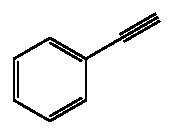
\includegraphics[max width=0.92\linewidth,max height=8.5cm]{qui/org_fenilacetileno}
\end{center}
{\centering\small\color{gris}Etinilbenceno (fórmula topológica)\par}
\alts{8 $\sigma$ (C--C), 5 $\pi$ (C--C) y 6 $\sigma$ (C--H)}{8 $\sigma$ (C--C), 2 $\pi$ (C--C) y 6 $\sigma$ (C--H)}{7 $\sigma$ (C--C), 5 $\pi$ (C--C) y 5 $\sigma$ (C--H)}{10 $\sigma$ (C--C), 5 $\pi$ (C--C) y 6 $\sigma$ (C--H)}
\solucion{\textbf{Paso 1. ¿Qué nos piden?} Tres conteos: enlaces $\sigma$ entre carbonos, enlaces $\pi$ entre carbonos y enlaces $\sigma$ C--H.

 

\textbf{Paso 2. Cuenta los carbonos.} El anillo tiene 6 vértices (6 C) y la cadena lateral tiene 2 C (el vértice unido al anillo y el extremo del triple). Total: 8 C, fórmula C\textsubscript{8}H\textsubscript{6}.

 

\textbf{Paso 3. Enlaces C--C y sus $\sigma$.} En el anillo hay 6 enlaces C--C; el anillo se une a la cadena con 1 enlace; y el triple es 1 enlace más. Son 8 enlaces C--C, y cada uno tiene exactamente 1 $\sigma$: \textbf{8 $\sigma$ (C--C)}.

 

\textbf{Paso 4. Enlaces $\pi$.} El anillo dibujado tiene 3 dobles (3 $\pi$) y el triple aporta 2 $\pi$: \textbf{5 $\pi$}.

 

\textbf{Paso 5. Enlaces C--H.} Completa a 4 enlaces cada C del anillo: el C unido a la cadena tiene 3 vecinos (2 del anillo y 1 de la cadena) y uno de esos enlaces es doble, así que ya suma 4 y no lleva H; los otros 5 C del anillo llevan 1 H cada uno. El C terminal del triple lleva 1 H (3 del triple + 1 H = 4). Total: \textbf{6 $\sigma$ (C--H)}.

 

\textbf{Respuesta:} 8 $\sigma$ (C--C), 5 $\pi$ (C--C) y 6 $\sigma$ (C--H).

 

\textbf{Comprobación:} la molécula tiene $8 + 6 = 14$ átomos y 1 anillo, así que debe tener $14 - 1 + 1 = 14$ enlaces $\sigma$ en total: $8 + 6 = 14$. \ding{52}

 

\textbf{¿Por qué no las otras?} "2 $\pi$" cuenta solo el triple y olvida los 3 dobles del anillo. "7 $\sigma$ y 5 C--H" olvida el enlace entre el anillo y la cadena, y el H del extremo del triple. "10 $\sigma$" cuenta el triple como 3 enlaces $\sigma$, pero un triple tiene 1 $\sigma$ y 2 $\pi$.

\textbf{\color{cienciaD}Para recordar.} Cada enlace (simple, doble o triple) aporta un solo sigma; los pi son las líneas extra: 1 por doble y 2 por triple.}{A}
\end{elejemplo}

%% =====================================================================
%% qui_representaciones
\section[Modelos de representación de moléculas]{Modelos de representación de moléculas}
\modcomun\ \ {\color{gris}\itshape Fórmula molecular, empírica, desarrollada, semidesarrollada, condensada y topológica, y los modelos de esferas y varillas y compacto: qué muestra cada una y cómo pasar de una a otra contando C e H.\par}
\subsection{Fórmula molecular y fórmula empírica}
La \textbf{fórmula molecular} dice qué átomos tiene una molécula y \textbf{cuántos exactamente}. El butano es C\textsubscript{4}H\textsubscript{10}: 4 C y 10 H.

 

La \textbf{fórmula empírica} da solo la \textbf{proporción mínima entera} entre los átomos. Se obtiene dividiendo todos los subíndices por su máximo común divisor (MCD).

 

\textbf{Paso 1.} Escribe la fórmula molecular: C\textsubscript{6}H\textsubscript{12}O\textsubscript{6} (glucosa).\par \textbf{Paso 2.} Busca el MCD de 6, 12 y 6: es 6.\par \textbf{Paso 3.} Divide: C\textsubscript{1}H\textsubscript{2}O\textsubscript{1} \ensuremath{\rightarrow} \textbf{CH\textsubscript{2}O}.

 
\begin{center}\small
\begin{tabular}{@{}lll@{}}
\toprule
\textbf{Compuesto} & \textbf{Molecular} & \textbf{Empírica} \\
\midrule
butano & C\textsubscript{4}H\textsubscript{10} & C\textsubscript{2}H\textsubscript{5} \\
benceno & C\textsubscript{6}H\textsubscript{6} & CH \\
etino & C\textsubscript{2}H\textsubscript{2} & CH \\
ácido etanoico & C\textsubscript{2}H\textsubscript{4}O\textsubscript{2} & CH\textsubscript{2}O \\
cloroformo & CHCl\textsubscript{3} & CHCl\textsubscript{3} \\
\bottomrule
\end{tabular}
\end{center}
  
\begin{clave}[{Ya es mínima}] Si el MCD es 1, la empírica es igual a la molecular. Le pasa al cloroformo (CHCl\textsubscript{3}), a la vanilina (C\textsubscript{8}H\textsubscript{8}O\textsubscript{3}) y al propano (C\textsubscript{3}H\textsubscript{8}).\end{clave}
 
\begin{ojo}[{Error típico}] Dividir solo algunos subíndices, o dividir aunque no den enteros. En C\textsubscript{8}H\textsubscript{8}O\textsubscript{3}, el 3 no se puede dividir por 8: la fórmula ya es empírica.\end{ojo}
 
\begin{ojo}[{Ojo}] Distintas sustancias pueden tener la misma empírica: el etino y el benceno son ambos CH. La empírica sola no identifica un compuesto.\end{ojo}
\subsection{Desarrollada, semidesarrollada, condensada y topológica}
Las fórmulas estructurales muestran, además, \textbf{cómo están unidos} los átomos. Mira las cuatro formas de escribir el butano:

 
\begin{center}
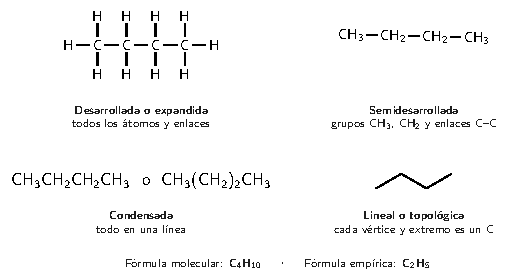
\includegraphics[max width=0.92\linewidth,max height=8.5cm]{qui/org_repr_butano}
\end{center}
  
\begin{itemize}
  \item \textbf{Desarrollada o expandida}: todos los átomos y todos los enlaces, uno por uno.
  \item \textbf{Semidesarrollada}: se agrupan los H con su carbono (CH\textsubscript{3}, CH\textsubscript{2}) y se dibujan los enlaces entre carbonos.
\end{itemize}
  
\begin{itemize}
  \item \textbf{Condensada}: todo en una línea, sin guiones; los grupos repetidos van entre paréntesis.
  \item \textbf{Lineal o topológica}: solo un zig-zag; cada vértice y cada extremo es un carbono.
\end{itemize}
\subsection{Cómo leer una fórmula topológica}
La fórmula topológica es la más usada en la PAES, porque es rápida de dibujar. Sus reglas:

 
\begin{itemize}
  \item Cada \textbf{vértice} y cada \textbf{extremo} de línea es un átomo de C.
  \item Los H unidos a carbono \textbf{no se dibujan}: cada C tiene los H que le faltan para llegar a 4 enlaces.
  \item Los otros átomos (O, N, Cl, S) \textbf{sí se escriben}, con sus H (OH, NH\textsubscript{2}).
  \item Una línea doble es un enlace doble; una triple, un triple.
\end{itemize}
 
\begin{center}
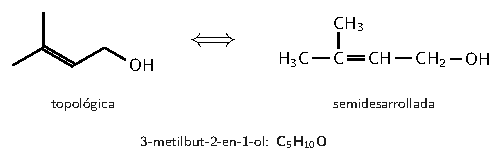
\includegraphics[max width=0.92\linewidth,max height=8.5cm]{qui/org_topo_prenol}
\end{center}
  
\begin{ejemplo}[{Ejemplo resuelto: contar C e H}] En la figura (3-metilbut-2-en-1-ol):\par \textbf{Paso 1. Carbonos.} 2 extremos arriba e izquierda + el vértice que los une + el vértice del doble + el vértice antes del OH = 5 C.\par \textbf{Paso 2. H de cada C} = 4 \ensuremath{-} (enlaces que ya tiene):\par · los dos CH\textsubscript{3} de los extremos: 3 + 3\par · el C con el doble y dos ramas: 4 \ensuremath{-} 4 = 0\par · el =CH--: 4 \ensuremath{-} 3 = 1\par · el CH\textsubscript{2} unido al OH: 4 \ensuremath{-} 2 = 2\par · el H del OH: 1\par \textbf{Paso 3.} Total: $3 + 3 + 0 + 1 + 2 + 1 = 10$ H. Fórmula: \textbf{C\textsubscript{5}H\textsubscript{10}O}.\end{ejemplo}
 
\begin{ojo}[{Errores típicos}] Olvidar los carbonos de los extremos, olvidar el H del OH, o poner H en un carbono que ya tiene 4 enlaces (por ejemplo, el que tiene un doble y dos ramas).\end{ojo}
\subsection{Modelos tridimensionales: esferas y varillas, y compacto}
\begin{center}
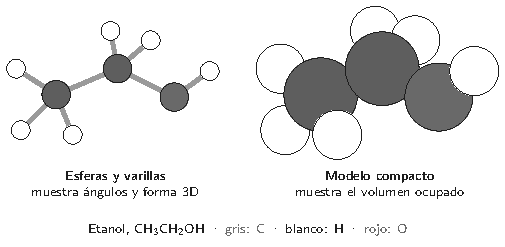
\includegraphics[max width=0.92\linewidth,max height=8.5cm]{qui/org_modelos}
\end{center}
  

\textbf{Modelo de esferas y varillas}: cada átomo es una esfera y cada enlace es una varilla. Muestra la \textbf{forma 3D}, los \textbf{ángulos de enlace} (109,5°, 120°, 180°) y cómo se ordenan los átomos en el espacio.

 

\textbf{Modelo compacto} (o de espacio lleno): las esferas se tocan y se superponen, a escala de su tamaño real. Muestra el \textbf{volumen} y la \textbf{forma externa} de la molécula, pero los enlaces y ángulos se ven poco.

  
\begin{clave}[{Colores habituales}] C: gris o negro · H: blanco · O: rojo · N: azul · Cl: verde.\end{clave}
 
\begin{ojo}[{Clave PAES}] Si dos formas de una molécula se diferencian solo en cómo se ordenan sus átomos \textbf{en el espacio}, ninguna fórmula escrita en el plano (molecular, empírica, condensada) las distingue: se necesita un modelo 3D, como el de esferas y varillas.\end{ojo}
\subsection{Comparar representaciones y moléculas}
\begin{center}\small
\begin{tabularx}{\linewidth}{@{}>{\raggedright\arraybackslash\hsize=1.29\hsize}X>{\raggedright\arraybackslash\hsize=1.29\hsize}X>{\raggedright\arraybackslash\hsize=0.67\hsize}X>{\raggedright\arraybackslash\hsize=0.76\hsize}X@{}}
\toprule
\textbf{Representación} & \textbf{¿Cuántos átomos de cada tipo?} & \textbf{¿Cómo se unen?} & \textbf{¿Forma 3D?} \\
\midrule
Empírica & solo la proporción & no & no \\
Molecular & sí & no & no \\
Condensada / semidesarrollada & sí & sí (por grupos) & no \\
Desarrollada / topológica & sí & sí & no (dibujo plano) \\
Esferas y varillas / compacto & sí & sí & sí \\
\bottomrule
\end{tabularx}
\end{center}
  
\begin{ejemplo}[{Ejemplo resuelto}] Etanol, CH\textsubscript{3}--CH\textsubscript{2}--OH, y metoximetano, CH\textsubscript{3}--O--CH\textsubscript{3}. \textbf{Paso 1.} Cuenta: los dos tienen 2 C, 6 H y 1 O: fórmula molecular C\textsubscript{2}H\textsubscript{6}O. \textbf{Paso 2.} Masa molar (H = 1, C = 12, O = 16): $2 \cdot 12 + 6 \cdot 1 + 16 = 46$ g/mol los dos. \textbf{Paso 3.} Pero la semidesarrollada muestra que son \textbf{distintos}: uno tiene O--H y el otro C--O--C. Son \textbf{isómeros}.\end{ejemplo}
  
\begin{ojo}[{Ojo con la masa molar}] Igual fórmula molecular implica igual masa molar. Pero igual masa molar \textbf{no} implica igual fórmula: el butan-2-ol (C\textsubscript{4}H\textsubscript{10}O) y el ácido propanoico (C\textsubscript{3}H\textsubscript{6}O\textsubscript{2}) pesan ambos 74 g/mol.\end{ojo}
\subsection{Lo clave del tema}
\begin{center}\small
\begin{tabularx}{\linewidth}{@{}>{\raggedright\arraybackslash\hsize=0.90\hsize}X>{\raggedright\arraybackslash\hsize=0.96\hsize}X>{\raggedright\arraybackslash\hsize=1.14\hsize}X@{}}
\toprule
\textbf{Representación} & \textbf{Butano} & \textbf{Lo que la distingue} \\
\midrule
Molecular & C\textsubscript{4}H\textsubscript{10} & número exacto de átomos \\
Empírica & C\textsubscript{2}H\textsubscript{5} & proporción mínima (divide por el MCD) \\
Desarrollada & todos los H y enlaces dibujados & todos los enlaces \\
Semidesarrollada & CH\textsubscript{3}--CH\textsubscript{2}--CH\textsubscript{2}--CH\textsubscript{3} & grupos CH\textsubscript{n} + enlaces C--C \\
Condensada & CH\textsubscript{3}(CH\textsubscript{2})\textsubscript{2}CH\textsubscript{3} & una línea, sin enlaces \\
Topológica & zig-zag de 4 vértices & vértices y extremos = C; H implícitos \\
Esferas y varillas / compacto & modelo 3D & ángulos / volumen \\
\bottomrule
\end{tabularx}
\end{center}
  
\begin{clave}[{Recuerda}] · En la fórmula topológica, cada extremo es un CH\textsubscript{3} (si no hay otro átomo escrito).\par · C\textsubscript{8}H\textsubscript{8}O\textsubscript{3} ya es empírica: el MCD de 8, 8 y 3 es 1.\par · Isómeros = misma fórmula molecular.\end{clave}
  
\begin{clave}[{Método PAES para contar}] 1. Marca cada vértice y extremo (C). 2. Para cada C: H = 4 \ensuremath{-} enlaces dibujados (doble cuenta 2, triple cuenta 3). 3. Suma los H de OH, NH\textsubscript{2}, CHO escritos. 4. Escribe C, H y luego los demás átomos. 5. Si piden la empírica, divide por el MCD.\end{clave}
\begin{elejemplo}{PAES Invierno 2026, adaptada}
Durante una clase de química orgánica, cuatro estudiantes analizan las estructuras de los compuestos X, Y y Z (masas atómicas: H = 1, C = 12, O = 16):

Luego, cada uno escribe en su cuaderno lo siguiente:

Estudiante 1: X e Y tienen la misma fórmula molecular.\par Estudiante 2: Z tiene más átomos de carbono que X.\par Estudiante 3: X y Z tienen la misma fórmula molecular, porque tienen la misma masa molar.\par Estudiante 4: Y tiene el doble de átomos de hidrógeno que Z.

¿Cuál de los estudiantes escribe una conclusión correcta?
\begin{center}
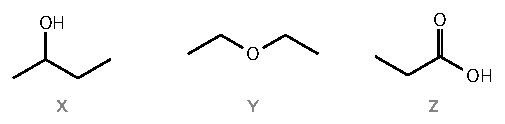
\includegraphics[max width=0.92\linewidth,max height=8.5cm]{qui/org_xyz}
\end{center}
\alts{El estudiante 1.}{El estudiante 2.}{El estudiante 3.}{El estudiante 4.}
\solucion{\textbf{Paso 1. ¿Qué nos piden?} La única afirmación correcta. Para eso necesitamos la fórmula molecular de X, Y y Z.

 

\textbf{Paso 2. Compuesto X.} Cuatro vértices/extremos: 4 C. H: extremo izquierdo CH\textsubscript{3} (3), vértice con OH: tiene 2 C y el O, le falta 1 H (1), siguiente vértice CH\textsubscript{2} (2), extremo CH\textsubscript{3} (3), más el H del OH (1). Total 10 H. \textbf{X = C\textsubscript{4}H\textsubscript{10}O} (butan-2-ol).

 

\textbf{Paso 3. Compuesto Y.} Dos C a cada lado del O: 4 C. Extremos CH\textsubscript{3} (3 + 3) y vértices junto al O, CH\textsubscript{2} (2 + 2). Total 10 H. \textbf{Y = C\textsubscript{4}H\textsubscript{10}O} (etoxietano).

 

\textbf{Paso 4. Compuesto Z.} 3 C: extremo CH\textsubscript{3} (3), vértice CH\textsubscript{2} (2) y el C del COOH (0 H sobre el C), más el H del OH (1). Total 6 H. \textbf{Z = C\textsubscript{3}H\textsubscript{6}O\textsubscript{2}} (ácido propanoico).

 

\textbf{Paso 5. Revisa cada estudiante.} 1: X e Y son ambos C\textsubscript{4}H\textsubscript{10}O. \ding{52} 2: Z tiene 3 C y X tiene 4. \ding{56} 3: X (C\textsubscript{4}H\textsubscript{10}O) y Z (C\textsubscript{3}H\textsubscript{6}O\textsubscript{2}) son fórmulas distintas. \ding{56} 4: Y tiene 10 H y Z tiene 6; el doble de 6 sería 12. \ding{56}

 

\textbf{Respuesta:} el estudiante 1.

 

\textbf{Comprobación:} masas molares: X = $4 \cdot 12 + 10 + 16 = 74$ g/mol; Z = $3 \cdot 12 + 6 + 2 \cdot 16 = 74$ g/mol. Tienen igual masa molar, pero distinta fórmula: por eso el estudiante 3 se equivoca, aunque su dato de masa sea cierto.

 

\textbf{¿Por qué no las otras?} El estudiante 2 no cuenta el carbono del extremo izquierdo de X o cuenta uno de más en Z. El estudiante 3 confunde "misma masa molar" con "misma fórmula". El estudiante 4 olvida que el doble de 6 es 12, no 10.

\textbf{\color{cienciaD}Para recordar.} Para comparar moléculas dibujadas, primero escribe la fórmula molecular de cada una: igual masa molar no significa igual fórmula.}{A}
\end{elejemplo}

%% =====================================================================
%% qui_hidrocarburos
\section[Hidrocarburos y nomenclatura IUPAC]{Hidrocarburos y nomenclatura IUPAC}
\modcomun\ \ {\color{gris}\itshape Alcanos, alquenos, alquinos, cíclicos y aromáticos: sus fórmulas generales, cómo encontrar la cadena principal, cómo numerarla y nombrar con ramificaciones, y qué son los isómeros.\par}
\subsection{Clasificación de los hidrocarburos}
Los \textbf{hidrocarburos} son compuestos formados \textbf{solo por C e H}. Son la base del petróleo, del gas natural y de los combustibles.

 
\begin{itemize}
  \item \textbf{Alifáticos} (cadena abierta, lineal o ramificada): 
\begin{itemize}
  \item \textbf{alcanos}: solo enlaces simples (\textbf{saturados}), sufijo \textbf{-ano};
  \item \textbf{alquenos}: al menos un C=C, sufijo \textbf{-eno};
  \item \textbf{alquinos}: al menos un C\ensuremath{\equiv}C, sufijo \textbf{-ino}.
\end{itemize}
  \item \textbf{Cíclicos}: la cadena se cierra en un anillo (prefijo \textbf{ciclo-}): ciclopropano, ciclohexano, ciclohexeno.
  \item \textbf{Aromáticos}: tienen el anillo del \textbf{benceno}.
\end{itemize}
 

Alquenos y alquinos son \textbf{insaturados}: tienen enlaces $\pi$ y dan reacciones de adición (por ejemplo, con H\textsubscript{2} o Br\textsubscript{2}).

  
\begin{center}
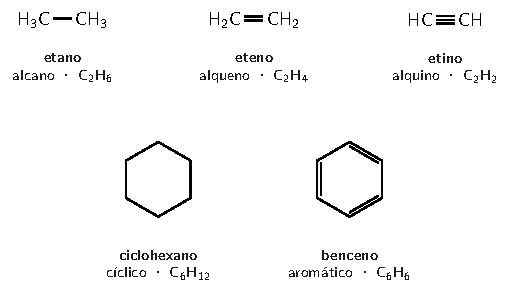
\includegraphics[max width=0.92\linewidth,max height=8.5cm]{qui/org_familias}
\end{center}
\subsection{Fórmulas generales y prefijos}
\begin{center}\small
\begin{tabular}{@{}lll@{}}
\toprule
\textbf{Familia} & \textbf{Fórmula general} & \textbf{Ejemplo} \\
\midrule
Alcano & C\textsubscript{n}H\textsubscript{2n+2} & propano C\textsubscript{3}H\textsubscript{8} \\
Alqueno (un doble) & C\textsubscript{n}H\textsubscript{2n} & propeno C\textsubscript{3}H\textsubscript{6} \\
Alquino (un triple) & C\textsubscript{n}H\textsubscript{2n\ensuremath{-}2} & propino C\textsubscript{3}H\textsubscript{4} \\
Cicloalcano & C\textsubscript{n}H\textsubscript{2n} & ciclopropano C\textsubscript{3}H\textsubscript{6} \\
Benceno & C\textsubscript{6}H\textsubscript{6} & --- \\
\bottomrule
\end{tabular}
\end{center}
 
\begin{clave}[{Regla de los 2 H}] Parte del alcano (C\textsubscript{n}H\textsubscript{2n+2}) y resta \textbf{2 H} por cada doble enlace o anillo, y \textbf{4 H} por cada triple. Ejemplo: C\textsubscript{6}H\textsubscript{10} = $14 - 4$: puede ser un hexino, un hexadieno o un ciclohexeno.\end{clave}
  
\begin{center}\small
\begin{tabular}{@{}llll@{}}
\toprule
\textbf{N.º de C} & \textbf{Prefijo} & \textbf{N.º de C} & \textbf{Prefijo} \\
\midrule
1 & met- & 6 & hex- \\
2 & et- & 7 & hept- \\
3 & prop- & 8 & oct- \\
4 & but- & 9 & non- \\
5 & pent- & 10 & dec- \\
\bottomrule
\end{tabular}
\end{center}
 
\begin{ojo}[{Ojo}] Un alqueno y un cicloalcano con los mismos C tienen la misma fórmula: el propeno y el ciclopropano son ambos C\textsubscript{3}H\textsubscript{6}.\end{ojo}
\subsection{Nombrar cadenas sin ramificar: la convención que usamos}
En este curso usamos las \textbf{recomendaciones IUPAC vigentes}, las mismas de las pruebas DEMRE: el número que indica la posición del doble o triple enlace (el \textbf{localizador}) va \textbf{justo antes del sufijo}.

 

\textbf{Paso 1.} Cuenta los C de la cadena que contiene el enlace múltiple: da el prefijo.\par \textbf{Paso 2.} Numera desde el extremo más cercano al enlace múltiple.\par \textbf{Paso 3.} Escribe prefijo + localizador + sufijo.

 
\begin{center}\small
\begin{tabular}{@{}ll@{}}
\toprule
\textbf{Estructura} & \textbf{Nombre} \\
\midrule
CH\textsubscript{2}=CH--CH\textsubscript{2}--CH\textsubscript{3} & but-1-eno \\
CH\textsubscript{3}--CH=CH--CH\textsubscript{3} & but-2-eno \\
CH\textsubscript{3}--C\ensuremath{\equiv}C--CH\textsubscript{2}--CH\textsubscript{3} & pent-2-ino \\
CH\textsubscript{2}=CH--CH=CH\textsubscript{2} & buta-1,3-dieno \\
\bottomrule
\end{tabular}
\end{center}
  
\begin{ojo}[{Nombres antiguos}] En libros más antiguos verás "2-buteno", "1-butino" o "2-pentino": son los \textbf{mismos compuestos} que but-2-eno, but-1-ino y pent-2-ino. Solo cambia dónde se escribe el número. En la PAES aparece la forma nueva ("penta-2-ino", "butan-2-ona").\end{ojo}
 
\begin{clave}[{Detalles de escritura}] Con dos dobles se agrega una "a" al prefijo: \textbf{buta}-1,3-dieno. Si hay doble y triple, el "-eno" va antes: pent-1-en-3-ino. Con 1 o 2 carbonos no hace falta localizador: eteno, etino, propeno.\end{clave}
 
\begin{clave}[{Grupos alquilo (ramificaciones)}] --CH\textsubscript{3} metil · --CH\textsubscript{2}CH\textsubscript{3} etil · --CH\textsubscript{2}CH\textsubscript{2}CH\textsubscript{3} propil · --CH(CH\textsubscript{3})\textsubscript{2} isopropil.\end{clave}
\subsection{Nombrar con ramificaciones, paso a paso}
\begin{center}
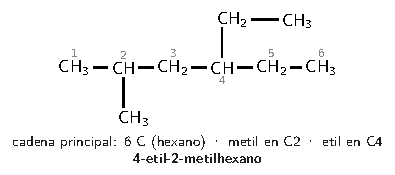
\includegraphics[max width=0.92\linewidth,max height=8.5cm]{qui/org_nom_ejemplo}
\end{center}
  

\textbf{Paso 1. Cadena principal.} La más larga (y, si hay dobles o triples, la que los contiene). Aquí: 6 C \ensuremath{\rightarrow} \textbf{hexano}. Ojo: la cadena más larga puede doblar por una ramificación; no tiene que ser la horizontal.

 

\textbf{Paso 2. Numera} desde el extremo que dé los números más bajos: primero al enlace múltiple; si no hay, a las ramificaciones. Desde la izquierda: 2 y 4. Desde la derecha: 3 y 5. Gana la izquierda.

 

\textbf{Paso 3. Nombra las ramificaciones}: metil en C2, etil en C4.

 

\textbf{Paso 4. Ordena alfabéticamente} (etil antes que metil) y escribe: \textbf{4-etil-2-metilhexano}.

  
\begin{clave}[{Más reglas}] · Ramificaciones repetidas: di-, tri-, tetra-: 2,3-dimetilbutano. Estos prefijos no cuentan para el orden alfabético.\par · Números con comas entre sí y guion entre número y letra: 2,2-dimetilpropano.\par · Si dos cadenas igual de largas compiten, se elige la que tiene más ramificaciones.\end{clave}
 
\begin{ejemplo}[{Ejemplo con doble enlace}] CH\textsubscript{2}=C(CH\textsubscript{3})--CH\textsubscript{2}--CH\textsubscript{3}: cadena de 4 C con el doble; se numera desde el doble (C1). Metil en C2: \textbf{2-metilbut-1-eno}.\end{ejemplo}
\subsection{Hidrocarburos cíclicos y aromáticos}
\textbf{Cicloalcanos}: anillos de C con solo enlaces simples. Se nombran con \textbf{ciclo-} + el nombre del alcano: ciclopropano, ciclopentano, ciclohexano (C\textsubscript{6}H\textsubscript{12}). Con una ramificación: metilciclohexano.

 

\textbf{Aromáticos}: contienen el \textbf{benceno}, C\textsubscript{6}H\textsubscript{6}. Se dibuja con tres dobles alternados o con un círculo dentro del hexágono: sus electrones $\pi$ están \textbf{deslocalizados} en todo el anillo. Por eso el benceno es muy estable y, a diferencia de los alquenos, da reacciones de \textbf{sustitución} y no de adición.

 

Los 6 C del benceno son sp², el anillo es plano y sus ángulos miden 120°.

  
\begin{center}\small
\begin{tabularx}{\linewidth}{@{}>{\raggedright\arraybackslash\hsize=0.97\hsize}X>{\raggedright\arraybackslash\hsize=0.42\hsize}X>{\raggedright\arraybackslash\hsize=1.61\hsize}X@{}}
\toprule
\textbf{Aromático} & \textbf{Fórmula} & \textbf{Uso} \\
\midrule
benceno & C\textsubscript{6}H\textsubscript{6} & materia prima industrial (tóxico) \\
tolueno (metilbenceno) & C\textsubscript{7}H\textsubscript{8} & solvente de pinturas \\
estireno (vinilbenceno) & C\textsubscript{8}H\textsubscript{8} & fabricación de plumavit (poliestireno) \\
naftaleno & C\textsubscript{10}H\textsubscript{8} & antiguas bolitas de naftalina \\
\bottomrule
\end{tabularx}
\end{center}
 
\begin{ojo}[{Error típico}] Contar 2 H en cada C del benceno, como si fuera ciclohexano. En el benceno cada C tiene 1 H (o 0 si lleva un sustituyente).\end{ojo}
\subsection{Isómeros y temperatura de ebullición}
Los \textbf{isómeros} tienen la \textbf{misma fórmula molecular} pero \textbf{distinta estructura}, y por eso distintas propiedades.

 
\begin{itemize}
  \item \textbf{De cadena}: cambia el esqueleto. Butano y metilpropano (C\textsubscript{4}H\textsubscript{10}).
  \item \textbf{De posición}: cambia la ubicación del doble enlace o del grupo. But-1-eno y but-2-eno.
  \item \textbf{De función}: cambia el tipo de compuesto. Etanol y metoximetano (C\textsubscript{2}H\textsubscript{6}O); hex-1-eno y ciclohexano (C\textsubscript{6}H\textsubscript{12}).
\end{itemize}
 
\begin{clave}[{Dos tendencias que pregunta la PAES}] 1. En una serie de alcanos lineales, \textbf{a más carbonos, mayor temperatura de ebullición} (más superficie de contacto entre moléculas).\par 2. Entre isómeros, \textbf{a más ramificación, menor temperatura de ebullición} (la molécula es más compacta y se atrae menos con sus vecinas).\end{clave}
  
\begin{center}
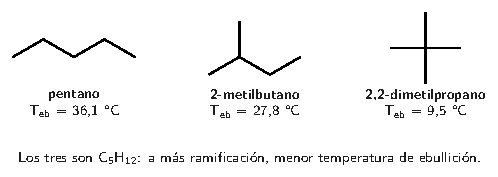
\includegraphics[max width=0.92\linewidth,max height=8.5cm]{qui/org_isomeros_c5}
\end{center}
 
\begin{ojo}[{Ojo}] "3-metilbutano" no existe como nombre: numerado bien, es el 2-metilbutano. Y "1-metilbutano" es en realidad el pentano. Antes de contar isómeros, nombra cada uno para no repetir.\end{ojo}
\subsection{Lo clave del tema}
\begin{center}\small
\begin{tabularx}{\linewidth}{@{}>{\raggedright\arraybackslash\hsize=0.95\hsize}X>{\raggedright\arraybackslash\hsize=1.08\hsize}X>{\raggedright\arraybackslash\hsize=0.95\hsize}X>{\raggedright\arraybackslash\hsize=0.95\hsize}X>{\raggedright\arraybackslash\hsize=1.08\hsize}X@{}}
\toprule
\textbf{Familia} & \textbf{Enlace clave} & \textbf{Fórmula} & \textbf{Sufijo} & \textbf{Ejemplo} \\
\midrule
Alcano & solo simples & C\textsubscript{n}H\textsubscript{2n+2} & -ano & 2-metilbutano \\
Alqueno & C=C & C\textsubscript{n}H\textsubscript{2n} & -eno & but-2-eno \\
Alquino & C\ensuremath{\equiv}C & C\textsubscript{n}H\textsubscript{2n\ensuremath{-}2} & -ino & pent-2-ino \\
Cicloalcano & anillo, simples & C\textsubscript{n}H\textsubscript{2n} & ciclo-\dots{}-ano & ciclohexano \\
Aromático & anillo bencénico & C\textsubscript{6}H\textsubscript{6} (benceno) & -benceno & metilbenceno \\
\bottomrule
\end{tabularx}
\end{center}
  
\begin{clave}[{Recuerda}] · La cadena principal es la más larga, aunque se doble.\par · Los sustituyentes van en orden alfabético: 4-etil-2-metilhexano.\par · El doble enlace lleva el número más bajo: pent-2-eno.\par · Isómeros = misma fórmula molecular.\end{clave}
  
\begin{clave}[{Método PAES para nombrar}] 1. Busca la cadena más larga que contenga el doble o triple. 2. Numera para que el enlace múltiple (o, si no hay, las ramas) tenga el número más bajo. 3. Identifica ramas y su posición. 4. Escribe en orden alfabético: localizador-rama + prefijo + localizador + sufijo. 5. Revisa: ¿el total de C del nombre coincide con el dibujo?\end{clave}
\begin{elejemplo}{PAES Invierno 2027, adaptada}
Respecto de la siguiente estructura de un hidrocarburo:

¿Cuál es su nombre correcto, según la IUPAC?
\begin{center}
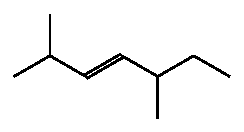
\includegraphics[max width=0.92\linewidth,max height=8.5cm]{qui/org_ej_nombre}
\end{center}
\alts{3,6-dimetilhept-4-eno}{2,5-dimetilheptano}{5-etil-2-metilhex-3-eno}{2,5-dimetilhept-3-eno}
\solucion{\textbf{Paso 1. ¿Qué nos piden?} El nombre IUPAC: cadena principal, numeración, ramificaciones y sufijo.

 

\textbf{Paso 2. Tipo de compuesto.} Solo C e H y una línea doble: es un \textbf{alqueno} (sufijo -eno).

 

\textbf{Paso 3. Cadena principal.} Busca la cadena más larga que contenga el doble enlace. Partiendo del extremo inferior izquierdo: 1 C, sube al vértice ramificado, baja, doble, sube, baja al otro vértice ramificado, y sigue por la derecha 2 C más. Son \textbf{7 C}: hept-. Las dos líneas que salen hacia arriba y hacia abajo de los vértices ramificados son metilos.

 

\textbf{Paso 4. Numeración.} Desde la izquierda, el doble enlace queda entre C3 y C4 \ensuremath{\rightarrow} localizador 3. Desde la derecha quedaría en 4. Gana la izquierda: \textbf{hept-3-eno}.

 

\textbf{Paso 5. Ramificaciones.} Con esa numeración, los metilos están en C2 y C5: \textbf{2,5-dimetil}.

 

\textbf{Respuesta:} 2,5-dimetilhept-3-eno.

 

\textbf{Comprobación:} el nombre indica $7 + 2 = 9$ C y el dibujo tiene 9 vértices y extremos. Fórmula: C\textsubscript{9}H\textsubscript{18} = C\textsubscript{n}H\textsubscript{2n}, como corresponde a un alqueno. \ding{52}

 

\textbf{¿Por qué no las otras?} "3,6-dimetilhept-4-eno" numera desde la derecha y le da al doble un número mayor (4 en vez de 3). "2,5-dimetilheptano" ignora el doble enlace (sería un alcano, C\textsubscript{9}H\textsubscript{20}). "5-etil-2-metilhex-3-eno" elige una cadena de 6 C cuando hay una de 7, y además deja una rama etilo que debería ser parte de la cadena.

\textbf{\color{cienciaD}Para recordar.} Cadena más larga con el doble enlace, numerada para que el doble tenga el número más bajo; luego las ramas en orden alfabético.}{D}
\end{elejemplo}

%% =====================================================================
%% qui_funcionales
\section[Grupos funcionales]{Grupos funcionales}
\modcomun\ \ {\color{gris}\itshape Haluros, alcoholes, fenoles, éteres, sulfuros, aldehídos, cetonas, ácidos carboxílicos, ésteres, anhídridos, amidas, aminas y nitrilos: cómo se escriben, cómo se nombran, cómo reconocerlos en fármacos y aromas, y para qué se usan.\par}
\subsection{¿Qué es un grupo funcional?}
Un \textbf{grupo funcional} es un átomo o grupo de átomos (casi siempre con O, N, S o un halógeno) que le da a la molécula sus propiedades químicas. Moléculas con el mismo grupo funcional se comportan de forma parecida.

 

Se escribe \textbf{R} para el resto de la molécula (la parte de C e H). Así, R--OH es "cualquier alcohol": CH\textsubscript{3}--OH, CH\textsubscript{3}--CH\textsubscript{2}--OH, etc.

 

Cuando una molécula tiene varios grupos, el de \textbf{mayor prioridad} da el sufijo del nombre y los demás se nombran como prefijos:

 
\begin{center}
\textbf{ácido carboxílico > anhídrido > éster > amida > nitrilo > aldehído > cetona > alcohol > amina > éter > haluro}
\end{center}
  
\begin{ejemplo}[{Ejemplo}] HO--CH\textsubscript{2}--CH\textsubscript{2}--CH\textsubscript{2}--COOH tiene un alcohol y un ácido. Manda el ácido: la cadena se numera desde el COOH (C1) y el OH queda en C4 como prefijo "hidroxi": \textbf{ácido 4-hidroxibutanoico}.\end{ejemplo}
 
\begin{ojo}[{Nombres comunes}] El temario acepta nombres IUPAC o comunes. Conviene saber los dos para los compuestos famosos: acetona = propanona, ácido acético = ácido etanoico, formaldehído = metanal, cloroformo = triclorometano.\end{ojo}
\subsection{Oxígeno con enlaces simples: alcoholes, fenoles y éteres}
\begin{center}
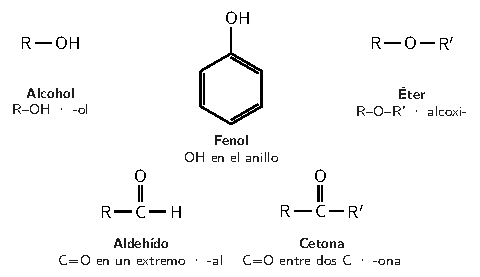
\includegraphics[max width=0.92\linewidth,max height=8.5cm]{qui/org_grupos_o}
\end{center}
  

\textbf{Alcohol, R--OH.} Sufijo \textbf{-ol}, con localizador: propan-2-ol. Ejemplos: metanol (tóxico), etanol (bebidas, alcohol gel, combustible), propan-2-ol (alcohol isopropílico, desinfectante), glicerol (cosméticos). Según el C que lleva el OH, son primarios (el C tiene 1 C vecino), secundarios (2) o terciarios (3). Forman \textbf{puentes de hidrógeno}: temperaturas de ebullición altas y los pequeños son solubles en agua.

 

\textbf{Fenol, OH unido a un anillo bencénico.} El fenol, C\textsubscript{6}H\textsubscript{5}OH, es desinfectante; los fenoles son antioxidantes y están en el timol del tomillo y en la vanilina. Son más ácidos que los alcoholes.

  

\textbf{Éter, R--O--R'.} El O está \textbf{entre dos carbonos}. IUPAC: el grupo pequeño con O se nombra "alcoxi": CH\textsubscript{3}--O--CH\textsubscript{2}--CH\textsubscript{3} es \textbf{metoxietano} (común: etil metil éter). El etoxietano (dietil éter) fue un anestésico y hoy es solvente. No forman puentes de hidrógeno entre sí: hierven a menor temperatura que el alcohol isómero.

 
\begin{ojo}[{Alcohol o fenol}] Si el OH está en un C del anillo bencénico, es fenol; si está en un C con solo enlaces simples, es alcohol.\end{ojo}
\subsection{El grupo carbonilo: aldehídos y cetonas}
El \textbf{carbonilo} es un C=O. Su posición define la familia:

 

\textbf{Aldehído, R--CHO.} El C=O está en un \textbf{extremo} de la cadena: el C lleva un H. Sufijo \textbf{-al}, sin número (el C del CHO siempre es C1): metanal, etanal, butanal. Ejemplos: metanal o formaldehído (la formalina conserva tejidos), benzaldehído (aroma de almendras), cinamaldehído (canela), vanilina (vainilla).

 

\textbf{Cetona, R--CO--R'.} El C=O está \textbf{entre dos carbonos}. Sufijo \textbf{-ona}, con localizador: pentan-2-ona, pentan-3-ona. La propanona (acetona) es el solvente del quitaesmalte; la butan-2-ona se usa en pinturas.

  
\begin{ejemplo}[{Ejemplo resuelto}] CH\textsubscript{3}--CH\textsubscript{2}--CH(CH\textsubscript{3})--CH\textsubscript{2}--CHO. \textbf{Paso 1.} Cadena más larga con el CHO: 5 C \ensuremath{\rightarrow} pentanal. \textbf{Paso 2.} El CHO es C1, así que el metilo queda en C3. \textbf{Nombre:} 3-metilpentanal. \textbf{Fórmula:} C\textsubscript{6}H\textsubscript{12}O.\end{ejemplo}
 
\begin{ojo}[{Error típico}] Llamar cetona a todo C=O. Mira los vecinos del carbono del C=O: si uno es H, es aldehído; si son dos C, es cetona; si uno es O o N, es ácido, éster o amida (siguiente sección).\end{ojo}
 
\begin{clave}[{Oxidación}] Alcohol primario \ensuremath{\rightarrow} aldehído \ensuremath{\rightarrow} ácido carboxílico. Alcohol secundario \ensuremath{\rightarrow} cetona.\end{clave}
\subsection{Ácidos carboxílicos y sus derivados: ésteres, anhídridos y amidas}
\begin{center}
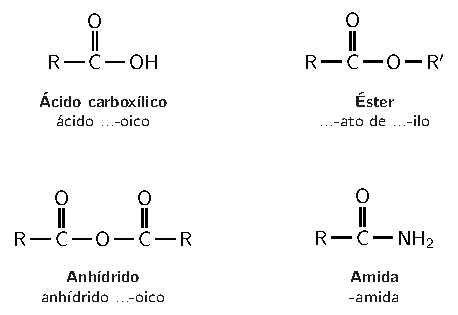
\includegraphics[max width=0.92\linewidth,max height=8.5cm]{qui/org_grupos_co}
\end{center}
  

\textbf{Ácido carboxílico, R--COOH.} "ácido \dots{}-oico": ácido metanoico (fórmico, de las hormigas), ácido etanoico (acético, del vinagre), ácido butanoico (mantequilla rancia). Son ácidos débiles y forman puentes de hidrógeno.

 

\textbf{Éster, R--COO--R'.} Se forma por \textbf{esterificación}: ácido + alcohol \ensuremath{\rightarrow} éster + agua. Nombre: la parte del ácido termina en \textbf{-ato} y la del alcohol en \textbf{-ilo}: CH\textsubscript{3}--COO--CH\textsubscript{2}--CH\textsubscript{3} es \textbf{etanoato de etilo} (acetato de etilo). Dan los \textbf{aromas frutales}: etanoato de 3-metilbutilo (plátano), butanoato de etilo (piña). Las grasas y aceites son ésteres.

  

\textbf{Anhídrido, R--CO--O--CO--R.} Dos grupos acilo unidos por un O (como dos ácidos que perdieron una molécula de agua). El anhídrido etanoico (acético) se usa para fabricar la aspirina.

 

\textbf{Amida, R--CO--NH\textsubscript{2}.} Sufijo \textbf{-amida}: etanamida. La urea es una amida; el \textbf{enlace peptídico} que une los aminoácidos en las proteínas es una amida, igual que el nailon y el paracetamol.

 
\begin{ojo}[{Éster o éter}] Los dos tienen C--O--C, pero el éster tiene además un C=O pegado a ese O. Sin C=O, es éter.\end{ojo}
\subsection{Nitrógeno, azufre y halógenos: aminas, nitrilos, sulfuros y haluros}
\begin{center}
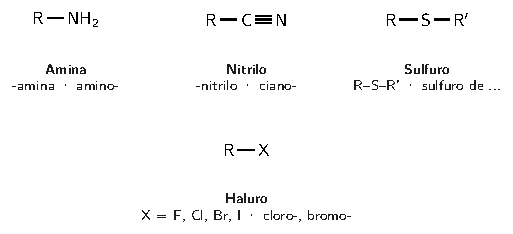
\includegraphics[max width=0.92\linewidth,max height=8.5cm]{qui/org_grupos_nsx}
\end{center}
  

\textbf{Amina, R--NH\textsubscript{2}} (también R\textsubscript{2}NH y R\textsubscript{3}N). Sufijo \textbf{-amina}: metanamina (metilamina). Son \textbf{básicas} y las pequeñas huelen a pescado. Están en los aminoácidos, la adrenalina, la anilina (colorantes) y alcaloides como la cafeína y la nicotina.

 

\textbf{Nitrilo, R--C\ensuremath{\equiv}N.} Sufijo \textbf{-nitrilo}, contando el C del CN: CH\textsubscript{3}--CN es etanonitrilo (acetonitrilo, un solvente). El propenonitrilo (acrilonitrilo) se usa para fibras acrílicas.

  

\textbf{Sulfuro (tioéter), R--S--R'.} Como un éter, pero con S: CH\textsubscript{3}--S--CH\textsubscript{3} es el sulfuro de dimetilo (olor a mar y a repollo cocido). El sulfuro de dialilo da parte del olor del ajo. No confundir con los tioles (R--SH), que se agregan al gas para detectar fugas.

 

\textbf{Haluro de alquilo, R--X} (X = F, Cl, Br, I). Se nombran con prefijos: clorometano, 2-bromopropano. El triclorometano (cloroformo) fue anestésico y hoy es solvente; los CFC dañan la capa de ozono; el PVC y el teflón son polímeros halogenados.
\subsection{Reconocer grupos en moléculas reales}
\begin{center}
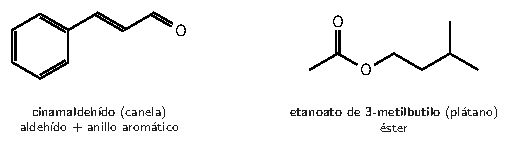
\includegraphics[max width=0.92\linewidth,max height=8.5cm]{qui/org_reales}
\end{center}
  

En la PAES aparecen fármacos, aromas e insecticidas dibujados en fórmula topológica. Para reconocer sus grupos, mira cada heteroátomo (O, N, S, halógeno) y a sus \textbf{vecinos}:

 
\begin{center}\small
\begin{tabular}{@{}ll@{}}
\toprule
\textbf{Lo que ves} & \textbf{Grupo} \\
\midrule
OH en C con solo simples & alcohol \\
OH en el anillo bencénico & fenol \\
C--O--C, sin C=O al lado & éter \\
C=O en un extremo (con H) & aldehído \\
C=O entre dos C & cetona \\
C=O con OH en el mismo C & ácido carboxílico \\
C=O con O--C en el mismo C & éster \\
C=O con N en el mismo C & amida \\
N con solo enlaces simples a C o H & amina \\
C\ensuremath{\equiv}N & nitrilo \\
\bottomrule
\end{tabular}
\end{center}
  
\begin{ejemplo}[{Ejemplo resuelto: paracetamol}] HO--C\textsubscript{6}H\textsubscript{4}--NH--CO--CH\textsubscript{3}. \textbf{Paso 1.} El OH está sobre el anillo: \textbf{fenol}. \textbf{Paso 2.} El N está unido a un C que tiene un C=O: no es amina, es \textbf{amida}. \textbf{Paso 3.} No hay ácido ni éster: el único C=O es parte de la amida.\end{ejemplo}
 
\begin{ojo}[{Error típico}] Mirar un átomo solo. Un O puede ser alcohol, éter, cetona, éster o ácido según sus vecinos, y un N puede ser amina o amida. Revisa siempre el carbono de al lado.\end{ojo}
\subsection{Lo clave del tema}
\begin{center}\small
\begin{tabularx}{\linewidth}{@{}>{\raggedright\arraybackslash\hsize=0.72\hsize}X>{\raggedright\arraybackslash\hsize=0.60\hsize}X>{\raggedright\arraybackslash\hsize=1.15\hsize}X>{\raggedright\arraybackslash\hsize=1.53\hsize}X@{}}
\toprule
\textbf{Grupo} & \textbf{Fórmula} & \textbf{Nombre (ejemplo)} & \textbf{Uso o característica} \\
\midrule
Haluro & R--X & triclorometano (cloroformo) & solventes, CFC, PVC \\
Alcohol & R--OH & etanol & bebidas, desinfectante; puentes de H \\
Fenol & Ar--OH & fenol & desinfectante, antioxidante \\
Éter & R--O--R' & etoxietano (dietil éter) & anestésico antiguo, solvente \\
Sulfuro & R--S--R' & sulfuro de dimetilo & olores (ajo, mar) \\
Aldehído & R--CHO & metanal (formaldehído) & conservante (formalina), aromas \\
Cetona & R--CO--R' & propanona (acetona) & solvente, quitaesmalte \\
Ácido carboxílico & R--COOH & ácido etanoico (acético) & vinagre; ácido débil \\
Éster & R--COO--R' & etanoato de etilo & aromas frutales, grasas \\
Anhídrido & R--CO--O--CO--R & anhídrido etanoico & síntesis de aspirina \\
Amida & R--CO--NH\textsubscript{2} & etanamida & proteínas, nailon, paracetamol \\
Amina & R--NH\textsubscript{2} & metanamina (metilamina) & básicas, olor a pescado, alcaloides \\
Nitrilo & R--C\ensuremath{\equiv}N & etanonitrilo (acetonitrilo) & solventes, fibras acrílicas \\
\bottomrule
\end{tabularx}
\end{center}
  
\begin{clave}[{Recuerda}] · En un C=O mira los vecinos: H (aldehído), 2 C (cetona), OH (ácido), O--C (éster), N (amida).\par · N--C=O es una amida.\par · Etanoato de propilo y propanoato de etilo son distintos: "-ato" es la parte del ácido (con el C=O) y "-ilo" la del alcohol.\end{clave}
  
\begin{clave}[{Método PAES}] 1. Encierra cada heteroátomo. 2. Mira sus vecinos y usa la tabla de la sección anterior. 3. Si te piden el nombre, busca el grupo de mayor prioridad: da el sufijo y fija la numeración (C1 en el CHO o el COOH). 4. Si te piden un uso, asocia: éster--aroma, amida--proteínas, cetona--acetona, ácido--vinagre, amina--olor a pescado.\end{clave}
\begin{elejemplo}{PAES Regular 2026, adaptada}
El ácido acetilsalicílico (aspirina) es uno de los analgésicos más usados del mundo. Su estructura es la siguiente:

¿Cuáles grupos funcionales están presentes en esta molécula, además del anillo aromático?
\begin{center}
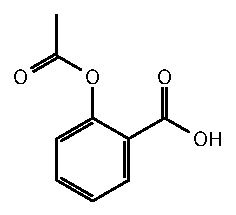
\includegraphics[max width=0.92\linewidth,max height=8.5cm]{qui/org_aspirina}
\end{center}
\alts{Cetona y éter}{Ácido carboxílico y éster}{Aldehído y alcohol}{Ácido carboxílico y cetona}
\solucion{\textbf{Paso 1. ¿Qué nos piden?} Nombrar los grupos funcionales que se ven en la estructura.

 

\textbf{Paso 2. Encierra los heteroátomos.} Hay 4 O, en dos grupos: uno a la derecha (C=O y OH) y otro arriba a la izquierda (un O unido al anillo y un C=O).

 

\textbf{Paso 3. Grupo de la derecha.} Un carbono tiene un C=O y un OH a la vez: es un \textbf{ácido carboxílico} (--COOH).

 

\textbf{Paso 4. Grupo de arriba.} El O unido al anillo está unido, del otro lado, a un C que tiene un C=O (y un CH\textsubscript{3}). Un O entre dos C, con C=O al lado: es un \textbf{éster} (--O--CO--CH\textsubscript{3}). No es éter, porque hay un C=O pegado; no es cetona, porque el C del C=O está unido a un O.

 

\textbf{Respuesta:} ácido carboxílico y éster.

 

\textbf{Comprobación:} la aspirina se fabrica haciendo reaccionar el ácido salicílico (que tiene un fenol) con anhídrido etanoico: el OH del fenol se convierte en el éster. Su fórmula es C\textsubscript{9}H\textsubscript{8}O\textsubscript{4}: los 4 O son los 2 del ácido y los 2 del éster. \ding{52}

 

\textbf{¿Por qué no las otras?} "Cetona y éter" mira el C=O y el C--O--C por separado, sin notar que están unidos: juntos son un éster. "Aldehído y alcohol" confunde el COOH con un CHO más un OH. "Ácido carboxílico y cetona" acierta el ácido, pero el otro C=O no está entre dos C: tiene un O al lado.

\textbf{\color{cienciaD}Para recordar.} Antes de nombrar un C=O o un O, mira a sus vecinos: juntos pueden formar un grupo distinto.}{B}
\end{elejemplo}

\chapter{Reacciones químicas y estequiometría}
%% =====================================================================
%% qui_leyes
\section[Leyes ponderales y balance de ecuaciones]{Leyes ponderales y balance de ecuaciones}
\modcomun\ \ {\color{gris}\itshape Las partes de una ecuación química, la conservación de la masa (Lavoisier), las proporciones definidas (Proust) y múltiples (Dalton), y cómo balancear una ecuación por tanteo.\par}
\subsection{Las partes de una ecuación química}
Una \textbf{reacción química} es un proceso en el que unas sustancias se transforman en otras distintas. Se escribe con una \textbf{ecuación química}:

 
\begin{center}
CH\textsubscript{4} (g) + 2 O\textsubscript{2} (g) \ensuremath{\rightarrow} CO\textsubscript{2} (g) + 2 H\textsubscript{2}O (l)
\end{center}
 

Se lee: «un metano gaseoso reacciona con dos oxígenos gaseosos y forma un dióxido de carbono gaseoso y dos aguas líquidas».

 
\begin{center}\small
\begin{tabularx}{\linewidth}{@{}>{\raggedright\arraybackslash\hsize=0.63\hsize}X>{\raggedright\arraybackslash\hsize=1.79\hsize}X>{\raggedright\arraybackslash\hsize=0.58\hsize}X@{}}
\toprule
\textbf{Parte} & \textbf{Qué es} & \textbf{En el ejemplo} \\
\midrule
Reactantes & lo que hay al comienzo, a la izquierda & CH\textsubscript{4} y O\textsubscript{2} \\
Productos & lo que se forma, a la derecha & CO\textsubscript{2} y H\textsubscript{2}O \\
Flecha & «reacciona y forma» & \ensuremath{\rightarrow} \\
Coeficiente & número \textbf{delante} de la fórmula: cuántas moléculas (o mol) & el 2 de 2 O\textsubscript{2} \\
Subíndice & número \textbf{pequeño abajo}: cuántos átomos hay en una molécula & el 4 de CH\textsubscript{4} \\
Estado & (s) sólido, (l) líquido, (g) gas, (ac) acuoso, disuelto en agua & (g), (l) \\
\bottomrule
\end{tabularx}
\end{center}
  
\begin{clave}[{Coeficiente por subíndice}] Para contar átomos, multiplica el coeficiente por el subíndice. En 2 H\textsubscript{2}O hay 2 moléculas de agua: $2\cdot 2 = 4$ átomos de H y $2\cdot 1 = 2$ átomos de O.\end{clave}
 
\begin{clave}[{Con paréntesis}] En 3 Ca(OH)\textsubscript{2} el 2 multiplica a todo el paréntesis: por fórmula hay 1 Ca, 2 O y 2 H. Con el coeficiente: 3 Ca, 6 O y 6 H.\end{clave}
 
\begin{ojo}[{Error típico}] Creer que el subíndice y el coeficiente significan lo mismo. 2 O (dos átomos de oxígeno sueltos) no es lo mismo que O\textsubscript{2} (una molécula de oxígeno), ni que 2 O\textsubscript{2} (dos moléculas, cuatro átomos).\end{ojo}
\subsection{Ley de conservación de la masa (Lavoisier)}
Antoine Lavoisier (siglo XVIII) masó con cuidado los reactantes y los productos de muchas reacciones hechas en recipientes cerrados y llegó a esta ley:

 
\begin{clave}[{Ley de Lavoisier}] En una reacción química, la masa total de los reactantes es igual a la masa total de los productos. La materia no se crea ni se destruye: se transforma.\end{clave}
 

\textbf{¿Por qué se cumple?} Mira el diagrama de partículas de 2 H\textsubscript{2} + O\textsubscript{2} \ensuremath{\rightarrow} 2 H\textsubscript{2}O. Los átomos solo se \textbf{reordenan}: se rompen unos enlaces y se forman otros, pero antes y después hay los mismos átomos (8 de H y 4 de O). Si los átomos son los mismos, la masa también.

 
\begin{center}
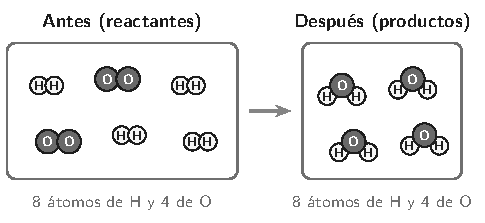
\includegraphics[max width=0.92\linewidth,max height=8.5cm]{qui/reac_particulas}
\end{center}
  
\begin{ejemplo}[{Ejemplo resuelto}] En un recipiente cerrado reaccionan completamente 12 g de magnesio con 8 g de oxígeno y se forma óxido de magnesio. ¿Qué masa de óxido se forma?\par \textbf{Paso 1.} Todo reaccionó: la masa de los reactantes es $12 + 8 = 20$ g.\par \textbf{Paso 2.} Por Lavoisier, la masa del producto es la misma: \textbf{20 g} de óxido de magnesio.\end{ejemplo}
 
\begin{clave}[{Si algo sobra}] Si en un recipiente cerrado pones 12 g de Mg y 10 g de O\textsubscript{2}, y se forman 20 g de óxido, la masa total sigue siendo $12 + 10 = 22$ g: son 20 g de óxido más $22 - 20 = 2$ g de oxígeno que \textbf{sobró} sin reaccionar.\end{clave}
 
\begin{ojo}[{Ojo}] Se conserva la \textbf{masa} y se conservan los \textbf{átomos}, pero no necesariamente el número de moléculas: en el diagrama hay 6 moléculas antes y 4 después.\end{ojo}
\subsection{Sistema abierto y sistema cerrado}
Cuando mezclas vinagre con bicarbonato se forma un gas, CO\textsubscript{2}. Si haces la reacción sobre una balanza, el resultado depende del recipiente:

 
\begin{center}
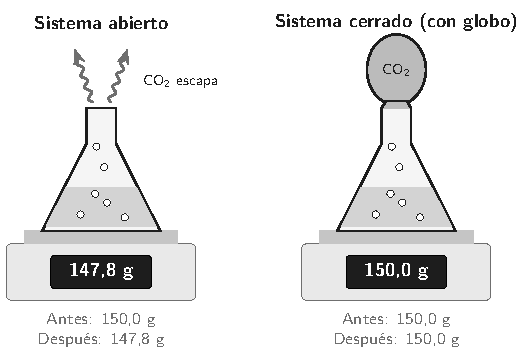
\includegraphics[max width=0.92\linewidth,max height=8.5cm]{qui/reac_balanza}
\end{center}
 

\textbf{Sistema abierto.} El CO\textsubscript{2} escapa al aire y la balanza ya no lo masa: marca 2,2 g menos. Esos 2,2 g son justamente el CO\textsubscript{2} que salió.

 

\textbf{Sistema cerrado.} El globo atrapa el gas. Nada entra ni sale y la balanza marca lo mismo antes y después.

  
\begin{ojo}[{Error típico}] Decir que en el sistema abierto «no se cumple la ley de Lavoisier». Sí se cumple: la masa no desapareció, se fue como gas. Para comprobar la ley hay que trabajar en un sistema cerrado o medir también el gas.\end{ojo}
 
\begin{ejemplo}[{Ejemplo resuelto}] Se calientan 10 g de carbonato de calcio en un crisol abierto: CaCO\textsubscript{3} (s) \ensuremath{\rightarrow} CaO (s) + CO\textsubscript{2} (g). Al final quedan 5,6 g de sólido (CaO). ¿Qué masa de CO\textsubscript{2} se liberó?\par \textbf{Paso 1.} Por Lavoisier: masa de CaCO\textsubscript{3} = masa de CaO + masa de CO\textsubscript{2}.\par \textbf{Paso 2.} $10 = 5{,}6 + m$, así que $m = 10 - 5{,}6 = 4{,}4$ g de CO\textsubscript{2}.\end{ejemplo}
 
\begin{clave}[{Al revés también pasa}] Si un metal se oxida en un recipiente abierto, el sólido \textbf{gana} masa: incorpora oxígeno del aire, que antes no estaba sobre la balanza.\end{clave}
\subsection{Ley de las proporciones definidas (Proust)}
\begin{clave}[{Ley de Proust}] Un compuesto siempre está formado por los mismos elementos combinados en la misma proporción en masa, sin importar cómo se obtuvo ni de dónde viene.\end{clave}
 

El agua pura siempre tiene 1 g de hidrógeno por cada 8 g de oxígeno (proporción en masa 1 : 8), sea de lluvia, de un río o hecha en el laboratorio.

 

\textbf{Consecuencia:} si mezclas los elementos en otra proporción, la reacción no cambia de proporción: uno de ellos \textbf{sobra} (queda en exceso).

 
\begin{center}\small
\begin{tabular}{@{}llll@{}}
\toprule
\textbf{Mg (g)} & \textbf{O (g)} & \textbf{Óxido formado (g)} & \textbf{Sobra} \\
\midrule
3 & 2 & 5 & nada \\
6 & 4 & 10 & nada \\
6 & 5 & 10 & 1 g de O \\
9 & 4 & 10 & 3 g de Mg \\
\bottomrule
\end{tabular}
\end{center}
  
\begin{ejemplo}[{Ejemplo resuelto}] El magnesio y el oxígeno se combinan en proporción 3 : 2. ¿Qué pasa si mezclas 9 g de Mg con 4 g de O?\par \textbf{Paso 1.} Para 4 g de O hacen falta $4\cdot\dfrac{3}{2} = 6$ g de Mg. Hay 9 g: alcanza y sobra.\par \textbf{Paso 2.} Reaccionan 6 g de Mg con 4 g de O y se forman $6 + 4 = 10$ g de óxido.\par \textbf{Paso 3.} Sobran $9 - 6 = 3$ g de Mg.\par \textbf{Comprobación:} masa inicial $9 + 4 = 13$ g; masa final $10 + 3 = 13$ g. \ding{52}\end{ejemplo}
 
\begin{ojo}[{Error típico}] Sumar todo lo que pusiste para obtener la masa del producto. Solo se suma lo que \textbf{reaccionó}; lo que sobra no forma producto.\end{ojo}
 
\begin{clave}[{En un gráfico}] Si graficas la masa de un elemento contra la masa del otro que se combina con él, obtienes una \textbf{recta que pasa por el origen}: la razón entre las masas es siempre la misma.\end{clave}
\subsection{Ley de las proporciones múltiples (Dalton)}
A veces dos elementos forman \textbf{más de un compuesto}. El carbono y el oxígeno forman CO y CO\textsubscript{2}; el azufre y el oxígeno forman SO\textsubscript{2} y SO\textsubscript{3}.

 
\begin{clave}[{Ley de Dalton}] Si dos elementos forman varios compuestos, las masas de uno de ellos que se combinan con una \textbf{misma masa} del otro están en una razón de números enteros sencillos.\end{clave}
 

\textbf{Cómo se aplica.} Fija la masa de un elemento y compara las masas del otro.

 
\begin{center}\small
\begin{tabular}{@{}lll@{}}
\toprule
\textbf{Compuesto} & \textbf{Masa de C (g)} & \textbf{Masa de O (g)} \\
\midrule
CO & 12 & 16 \\
CO\textsubscript{2} & 12 & 32 \\
\bottomrule
\end{tabular}
\end{center}
 

Con los mismos 12 g de C, las masas de O son 16 g y 32 g: razón $16 : 32 = 1 : 2$, números enteros sencillos.

  
\begin{ejemplo}[{Ejemplo resuelto}] En SO\textsubscript{2} hay 32 g de S por cada 32 g de O, y en SO\textsubscript{3} hay 32 g de S por cada 48 g de O. Con la misma masa de S, las masas de O están en razón $32 : 48 = 2 : 3$. \ding{52} Se cumple la ley.\end{ejemplo}
 
\begin{ojo}[{Ojo con los porcentajes}] Cada compuesto tiene su propio porcentaje fijo (Proust), pero compuestos distintos de los mismos elementos tienen porcentajes distintos. En CO hay $\dfrac{12}{28}\approx 43\%$ de C y en CO\textsubscript{2}, $\dfrac{12}{44}\approx 27\%$. Si en dos experimentos con hierro y oxígeno el porcentaje de hierro es distinto, se formaron dos óxidos distintos.\end{ojo}
 
\begin{clave}[{Las tres leyes juntas}] Las leyes ponderales llevaron a Dalton a su teoría atómica: los átomos se combinan en números enteros, se reordenan en las reacciones y no se crean ni se destruyen.\end{clave}
\subsection{Balancear una ecuación}
\textbf{Balancear} es elegir los coeficientes para que haya el mismo número de átomos de cada elemento a los dos lados. Así la ecuación cumple la ley de Lavoisier.

 

\textbf{Ejemplo:} C\textsubscript{3}H\textsubscript{8} + O\textsubscript{2} \ensuremath{\rightarrow} CO\textsubscript{2} + H\textsubscript{2}O.

 

\textbf{Paso 1. Carbono.} Hay 3 C a la izquierda: pon 3 delante del CO\textsubscript{2}.

 

\textbf{Paso 2. Hidrógeno.} Hay 8 H a la izquierda; cada agua tiene 2: pon 4 delante del H\textsubscript{2}O.

 

\textbf{Paso 3. Oxígeno, al final.} A la derecha hay $3\cdot 2 + 4\cdot 1 = 10$ átomos de O; cada O\textsubscript{2} tiene 2: pon 5 delante del O\textsubscript{2}.

 

\textbf{Resultado:} C\textsubscript{3}H\textsubscript{8} + 5 O\textsubscript{2} \ensuremath{\rightarrow} 3 CO\textsubscript{2} + 4 H\textsubscript{2}O.

 
\begin{center}\small
\begin{tabular}{@{}lll@{}}
\toprule
\textbf{Átomo} & \textbf{Izquierda} & \textbf{Derecha} \\
\midrule
C & 3 & 3 \\
H & 8 & $4\cdot 2 = 8$ \\
O & $5\cdot 2 = 10$ & $6 + 4 = 10$ \\
\bottomrule
\end{tabular}
\end{center}
  
\begin{clave}[{Orden práctico}] 1. Metales. 2. No metales distintos de H y O. 3. Hidrógeno. 4. Oxígeno al final. Si un grupo como NO\textsubscript{3} o SO\textsubscript{4} pasa entero de un lado al otro, cuéntalo como un bloque.\end{clave}
 
\begin{clave}[{Con número impar}] Al + O\textsubscript{2} \ensuremath{\rightarrow} Al\textsubscript{2}O\textsubscript{3}. Para tener O par a los dos lados, pon 2 Al\textsubscript{2}O\textsubscript{3} (6 O): necesitas 3 O\textsubscript{2}. Luego hay 4 Al a la derecha: 4 Al. Queda 4 Al + 3 O\textsubscript{2} \ensuremath{\rightarrow} 2 Al\textsubscript{2}O\textsubscript{3}.\end{clave}
 
\begin{ojo}[{Nunca cambies un subíndice}] Cambiar H\textsubscript{2}O por H\textsubscript{2}O\textsubscript{2} «para que cuadre» cambia la sustancia: el agua oxigenada no es agua. Solo se cambian los coeficientes, y se usan los enteros más pequeños posibles.\end{ojo}
\subsection{Lo clave del tema}
\begin{center}\small
\begin{tabularx}{\linewidth}{@{}>{\raggedright\arraybackslash\hsize=0.39\hsize}X>{\raggedright\arraybackslash\hsize=1.30\hsize}X>{\raggedright\arraybackslash\hsize=1.30\hsize}X@{}}
\toprule
\textbf{Ley o idea} & \textbf{Qué dice} & \textbf{Cómo se usa} \\
\midrule
Lavoisier & masa de reactantes = masa de productos & resta para hallar la masa que falta o la que sobró \\
Proust & cada compuesto tiene una proporción en masa fija & regla de tres con la proporción; lo que no calza, sobra \\
Dalton & con una masa fija de un elemento, las masas del otro están en razón entera & fija un elemento y divide las masas del otro \\
Balance & mismos átomos a ambos lados & cambia coeficientes, nunca subíndices \\
\bottomrule
\end{tabularx}
\end{center}
 
\begin{clave}[{Recuerda}] · Lo que sobra no forma producto: con 9 g de Mg y 4 g de O reaccionan 6 g + 4 g, se forman 10 g de óxido y sobran 3 g de Mg.\par · Si en un sistema abierto la masa baja, la que falta es el gas que escapó: Lavoisier se cumple.\par · En 2 H\textsubscript{2}O hay $2\cdot 2 = 4$ H.\par · Se balancea con coeficientes, nunca con subíndices: 2 H\textsubscript{2} + O\textsubscript{2} \ensuremath{\rightarrow} 2 H\textsubscript{2}O.\par · En los diagramas de partículas, escribe las moléculas tal como aparecen (X\textsubscript{2}) y no cuentes las que sobran.\end{clave}
 
\begin{clave}[{Método PAES}] 1. Escribe qué reacciona y qué se forma. 2. Si hay masas, usa Lavoisier (suma o resta) y Proust (proporción fija). 3. Si hay coeficientes, cuenta átomos elemento por elemento con una tabla izquierda/derecha. 4. En un diagrama, cuenta moléculas antes y después, descuenta las que sobran y simplifica. 5. Comprueba que la masa total, o los átomos, sean iguales a ambos lados.\end{clave}
\begin{elejemplo}{PAES Invierno 2026, adaptada}
Dos sustancias, X e Y, reaccionan para formar un único compuesto Z. Se realizaron tres ensayos y se registraron las masas iniciales de X e Y, la masa final de Z y el reactivo que quedó en exceso:
\begin{center}\small
\begin{tabular}{@{}lllll@{}}
\toprule
\textbf{Ensayo} & \textbf{Masa de X (g)} & \textbf{Masa de Y (g)} & \textbf{Masa de Z (g)} & \textbf{Exceso} \\
\midrule
\textbf{1} & 14 & 4 & 18 & nada \\
\textbf{2} & 7 & 4 & 9 & 2 g de Y \\
\textbf{3} & 20 & 4 & 18 & 6 g de X \\
\bottomrule
\end{tabular}
\end{center}
\altslargas{En los tres ensayos, la suma de las masas iniciales de X e Y es igual a la masa final de Z.}{7 g de X reaccionan exactamente con 4 g de Y.}{Para formar Z, las sustancias X e Y se combinan en una proporción en masa de 7 : 2.}{20 g de X reaccionan exactamente con 4 g de Y.}
\solucion{\textbf{Paso 1. ¿Qué nos piden?} La afirmación correcta sobre cómo se combinan X e Y. La clave es el ensayo en que no sobra nada: ahí todo lo que se puso reaccionó.

\textbf{Paso 2. Ensayo 1, sin exceso.} Reaccionaron 14 g de X con 4 g de Y y se formaron $14 + 4 = 18$ g de Z. \ding{52} Se cumple Lavoisier.

\textbf{Paso 3. La proporción.} $14 : 4$. Dividimos ambos por 2: $7 : 2$. Por cada 7 g de X reaccionan 2 g de Y.

\textbf{Paso 4. Revisa el ensayo 2 con la proporción.} Hay 7 g de X: necesitan 2 g de Y. Se pusieron 4 g, así que sobran $4 - 2 = 2$ g de Y y se forman $7 + 2 = 9$ g de Z. Coincide con la tabla. \ding{52}

\textbf{Paso 5. Revisa el ensayo 3.} Hay 4 g de Y: necesitan 14 g de X. Se pusieron 20 g, así que sobran $20 - 14 = 6$ g de X y se forman 18 g de Z. Coincide. \ding{52}

\textbf{Respuesta:} X e Y se combinan en proporción en masa 7 : 2 (ley de Proust).

\textbf{Comprobación:} en cada ensayo, masa inicial = masa de Z + exceso. Ensayo 2: $7 + 4 = 11$ y $9 + 2 = 11$. Ensayo 3: $20 + 4 = 24$ y $18 + 6 = 24$. \ding{52} La masa total se conserva, contando lo que sobró.

\textbf{¿Por qué no las otras?} La primera olvida el exceso: en el ensayo 2, $7 + 4 = 11$ g, pero solo se forman 9 g de Z porque sobran 2 g de Y. La segunda lee el ensayo 2 como si todo reaccionara, pero ahí sobró Y: 7 g de X reaccionan con 2 g de Y, no con 4. La cuarta lee el ensayo 3 sin descontar el exceso: de los 20 g de X solo reaccionaron 14.

\textbf{\color{cienciaD}Para recordar.} La proporción de combinación se lee en el ensayo donde no sobra nada; en los demás, masa inicial = producto + exceso.}{C}
\end{elejemplo}

%% =====================================================================
%% qui_mol
\section[El mol y la masa molar]{El mol y la masa molar}
\modcomun\ \ {\color{gris}\itshape Qué es un mol y el número de Avogadro, cómo calcular una masa molar, y cómo pasar de masa a cantidad de sustancia, a número de moléculas y a número de átomos.\par}
\subsection{Contar por montones: el mol}
Los átomos y las moléculas son tan pequeños que en una gota de agua hay miles de trillones. Para no trabajar con números gigantes, los químicos cuentan por «montones», igual que contamos huevos por docena.

 
\begin{clave}[{El mol}] Un \textbf{mol} es la cantidad de sustancia que contiene $6{,}02\cdot 10^{23}$ partículas. Ese número se llama \textbf{número de Avogadro}, $N_A$.\end{clave}
 

Una docena son 12 cosas, sean huevos o lápices. Un mol son $6{,}02\cdot 10^{23}$ partículas, sean átomos, moléculas o iones:

 
\begin{itemize}
  \item 1 mol de átomos de Fe = $6{,}02\cdot 10^{23}$ átomos de Fe.
  \item 1 mol de moléculas de H\textsubscript{2}O = $6{,}02\cdot 10^{23}$ moléculas de agua.
  \item 2 mol de CO\textsubscript{2} = $2\cdot 6{,}02\cdot 10^{23} = 1{,}204\cdot 10^{24}$ moléculas.
\end{itemize}
  
\begin{clave}[{Nombre y unidad}] La magnitud se llama \textbf{cantidad de sustancia}, se simboliza $n$ y su unidad es el \textbf{mol}. Es una de las unidades básicas del Sistema Internacional.\end{clave}
 
\begin{clave}[{Mitades y dobles}] $0{,}5$ mol son $3{,}01\cdot 10^{23}$ partículas; $1{,}5$ mol son $9{,}03\cdot 10^{23}$; $3$ mol son $1{,}806\cdot 10^{24}$. En la PAES los números se eligen para que estas cuentas salgan sin calculadora.\end{clave}
 
\begin{ojo}[{Error típico}] Pensar que un mol de cualquier sustancia tiene la misma masa. Un mol de huevos y un mol de sandías tienen el mismo número de unidades, pero no pesan lo mismo. Lo mismo pasa con un mol de H\textsubscript{2} y un mol de CO\textsubscript{2}.\end{ojo}
\subsection{Masa atómica y masa molar}
La \textbf{masa molar} ($M$) es la masa de un mol de una sustancia, en g/mol. Se calcula sumando las masas atómicas de todos los átomos de la fórmula (la PAES las entrega en la tabla periódica o en el enunciado).

 

\textbf{Ejemplo: agua, H\textsubscript{2}O.} 2 H y 1 O: $M = 2\cdot 1 + 16 = 18$ g/mol.

 

\textbf{Ejemplo: carbonato de calcio, CaCO\textsubscript{3}.} 1 Ca, 1 C y 3 O: $M = 40 + 12 + 3\cdot 16 = 100$ g/mol.

 

\textbf{Ejemplo: glucosa, C\textsubscript{6}H\textsubscript{12}O\textsubscript{6}.} $M = 6\cdot 12 + 12\cdot 1 + 6\cdot 16 = 72 + 12 + 96 = 180$ g/mol.

 
\begin{center}\small
\begin{tabular}{@{}lll@{}}
\toprule
\textbf{Sustancia} & \textbf{Cuenta} & \textbf{$M$ (g/mol)} \\
\midrule
O\textsubscript{2} & $2\cdot 16$ & 32 \\
CO\textsubscript{2} & $12 + 2\cdot 16$ & 44 \\
NH\textsubscript{3} & $14 + 3\cdot 1$ & 17 \\
NaCl & $23 + 35{,}5$ & 58,5 \\
H\textsubscript{2}SO\textsubscript{4} & $2 + 32 + 64$ & 98 \\
\bottomrule
\end{tabular}
\end{center}
  
\begin{clave}[{Con paréntesis}] Ca(OH)\textsubscript{2} tiene 1 Ca, 2 O y 2 H: $M = 40 + 2\cdot 16 + 2\cdot 1 = 74$ g/mol.\end{clave}
 
\begin{ojo}[{Error típico}] Olvidar el subíndice del paréntesis: $40 + 16 + 1 = 57$ g/mol para Ca(OH)\textsubscript{2} está mal. El 2 multiplica al O y al H.\end{ojo}
 
\begin{ojo}[{Fórmulas condensadas}] En CH\textsubscript{3}OH hay que juntar todos los H: $3 + 1 = 4$. $M = 12 + 4\cdot 1 + 16 = 32$ g/mol. Contar solo los 3 del CH\textsubscript{3} es un error frecuente.\end{ojo}
 
\begin{clave}[{Más átomos no es más masa}] El CH\textsubscript{4} tiene 5 átomos y $M = 16$ g/mol; el HCl tiene 2 átomos y $M = 36{,}5$ g/mol. Lo que manda es la masa de cada átomo, no cuántos hay.\end{clave}
\subsection{De masa a mol y de mol a masa}
\begin{center}
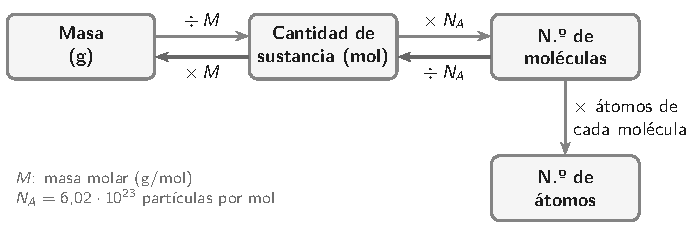
\includegraphics[max width=0.92\linewidth,max height=8.5cm]{qui/reac_mapa_mol}
\end{center}
 

La masa molar es el puente entre lo que se mide en la balanza (gramos) y lo que se cuenta (mol):

 
\begin{center}
$n = \dfrac{m}{M}$ y $m = n\cdot M$
\end{center}
  
\begin{ejemplo}[{Ejemplo resuelto 1}] ¿Cuántos mol hay en 88 g de CO\textsubscript{2}? ($M = 44$ g/mol)\par $n = \dfrac{88}{44} = 2$ mol.\end{ejemplo}
 
\begin{ejemplo}[{Ejemplo resuelto 2}] ¿Qué masa tienen 0,5 mol de glucosa? ($M = 180$ g/mol)\par $m = 0{,}5\cdot 180 = 90$ g.\end{ejemplo}
 
\begin{ejemplo}[{Ejemplo resuelto 3}] ¿Cuántos mol hay en 4,9 g de H\textsubscript{2}SO\textsubscript{4}? ($M = 98$ g/mol)\par $n = \dfrac{4{,}9}{98} = 0{,}05$ mol.\end{ejemplo}
 
\begin{ojo}[{Revisa las unidades}] g ÷ (g/mol) = mol. Si te queda «mol²/g» o «g²/mol», dividiste al revés. Un control rápido: si la masa es menor que $M$, tienes menos de 1 mol.\end{ojo}
\subsection{Moléculas y átomos dentro de las moléculas}
Para contar partículas se multiplica por el número de Avogadro: $N = n\cdot N_A$.

 

Pero cuidado: una molécula tiene varios átomos. En 2 mol de H\textsubscript{2}O:

 
\begin{center}\small
\begin{tabular}{@{}lll@{}}
\toprule
\textbf{Qué se cuenta} & \textbf{mol} & \textbf{Número} \\
\midrule
moléculas de H\textsubscript{2}O & 2 & $1{,}204\cdot 10^{24}$ \\
átomos de H & $2\cdot 2 = 4$ & $2{,}408\cdot 10^{24}$ \\
átomos de O & $2\cdot 1 = 2$ & $1{,}204\cdot 10^{24}$ \\
átomos en total & $2\cdot 3 = 6$ & $3{,}612\cdot 10^{24}$ \\
\bottomrule
\end{tabular}
\end{center}
  
\begin{ejemplo}[{Ejemplo resuelto}] ¿Cuántos átomos de hidrógeno hay en 8 g de metano, CH\textsubscript{4}? ($M = 16$ g/mol)\par \textbf{Paso 1.} Mol de CH\textsubscript{4}: $\dfrac{8}{16} = 0{,}5$ mol.\par \textbf{Paso 2.} Cada molécula tiene 4 H: $0{,}5\cdot 4 = 2$ mol de átomos de H.\par \textbf{Paso 3.} $2\cdot 6{,}02\cdot 10^{23} = 1{,}204\cdot 10^{24}$ átomos de H.\end{ejemplo}
 
\begin{ojo}[{Error típico}] Responder el número de \textbf{moléculas} cuando preguntan por \textbf{átomos} (o al revés). Subraya en el enunciado qué partícula te piden contar.\end{ojo}
\subsection{Comparar muestras}
Muchas preguntas comparan dos o más muestras. Hay dos situaciones típicas:

 

\textbf{Mismo número de moléculas (misma cantidad de sustancia).} Pesa más la sustancia de mayor masa molar. 1 mol de CO\textsubscript{2} (44 g) pesa más que 1 mol de H\textsubscript{2}O (18 g), aunque las dos muestras tengan $6{,}02\cdot 10^{23}$ moléculas.

 

\textbf{Misma masa.} Tiene más moléculas la sustancia de \textbf{menor} masa molar, porque cada molécula pesa menos. En 32 g de CH\textsubscript{4} hay 2 mol; en 32 g de O\textsubscript{2}, solo 1 mol.

 
\begin{center}\small
\begin{tabularx}{\linewidth}{@{}>{\raggedright\arraybackslash\hsize=0.84\hsize}X>{\raggedright\arraybackslash\hsize=1.16\hsize}X@{}}
\toprule
\textbf{Si las muestras tienen igual\dots{}} & \textbf{Entonces tiene más masa / más moléculas\dots{}} \\
\midrule
cantidad de sustancia (mol) & más masa: la de mayor $M$ \\
masa (g) & más moléculas: la de menor $M$ \\
\bottomrule
\end{tabularx}
\end{center}
  
\begin{ejemplo}[{Ejemplo resuelto}] 0,5 mol de O\textsubscript{3} y 0,75 mol de O\textsubscript{2}. ¿Tienen los mismos átomos de oxígeno?\par O\textsubscript{3}: $0{,}5\cdot 3 = 1{,}5$ mol de átomos. O\textsubscript{2}: $0{,}75\cdot 2 = 1{,}5$ mol de átomos. Sí, y por eso también tienen la misma masa: $1{,}5\cdot 16 = 24$ g. Pero el número de moléculas es distinto.\end{ejemplo}
 
\begin{ojo}[{Ojo}] «Igual número de moléculas» no implica «igual número de átomos»: 1 mol de CH\textsubscript{4} tiene 5 mol de átomos y 1 mol de O\textsubscript{2}, solo 2.\end{ojo}
\subsection{Lo clave del tema}
\begin{center}\small
\begin{tabularx}{\linewidth}{@{}>{\raggedright\arraybackslash\hsize=0.62\hsize}X>{\raggedright\arraybackslash\hsize=0.82\hsize}X>{\raggedright\arraybackslash\hsize=1.56\hsize}X@{}}
\toprule
\textbf{Quiero pasar de\dots{}} & \textbf{a\dots{}} & \textbf{Hago} \\
\midrule
masa (g) & mol & $n = \dfrac{m}{M}$ \\
mol & masa (g) & $m = n\cdot M$ \\
mol & moléculas & $N = n\cdot 6{,}02\cdot 10^{23}$ \\
moléculas & átomos de un elemento & multiplico por el subíndice de ese elemento \\
\bottomrule
\end{tabularx}
\end{center}
 
\begin{clave}[{Recuerda}] · $M$ de Ca(OH)\textsubscript{2} = $40 + 2\cdot 17 = 74$ g/mol.\par · $n = \dfrac{m}{M}$: 88 g de una sustancia de 44 g/mol son $\dfrac{88}{44} = 2$ mol.\par · En 1 mol de NH\textsubscript{3} hay $3\cdot 6{,}02\cdot 10^{23}$ átomos de H.\par · La masa la decide $M$, no el número de átomos: CH\textsubscript{4} tiene 16 g/mol y HCl 36,5 g/mol.\par · Igual masa no es igual cantidad: 32 g de O\textsubscript{2} son 1 mol y 32 g de CH\textsubscript{4} son 2 mol.\end{clave}
 
\begin{clave}[{Método PAES}] 1. Calcula la masa molar con cuidado (paréntesis y todos los H). 2. Pasa todo a mol: es la moneda común de la química. 3. Si piden partículas, multiplica por $N_A$, y si piden átomos, también por el subíndice. 4. Revisa las unidades y si el resultado tiene sentido (menos masa que $M$ es menos de 1 mol).\end{clave}
\begin{elejemplo}{PAES Invierno 2027, adaptada}
Si se dispone de $3{,}01\cdot 10^{23}$ moléculas de cada uno de los siguientes compuestos, ¿cuál de ellos tiene la mayor masa?

Masas atómicas (g/mol): H = 1; C = 12; S = 32; Cl = 35,5.
\alts{CH\textsubscript{4}}{C\textsubscript{2}H\textsubscript{6}}{H\textsubscript{2}S}{HCl}
\solucion{\textbf{Paso 1. ¿Qué nos piden?} Cuál de las cuatro muestras pesa más. Todas tienen el mismo número de moléculas, así que todas tienen la misma cantidad de sustancia.

\textbf{Paso 2. Pasa las moléculas a mol.} $n = \dfrac{3{,}01\cdot 10^{23}}{6{,}02\cdot 10^{23}} = 0{,}5$ mol de cada compuesto.

\textbf{Paso 3. Idea clave.} Con la misma cantidad de sustancia, pesa más la muestra cuya molécula pesa más: la de mayor masa molar. No hace falta calcular las masas, basta comparar $M$.

\textbf{Paso 4. Calcula las masas molares.}

\begin{itemize}
  \item CH\textsubscript{4}: $12 + 4\cdot 1 = 16$ g/mol.
  \item C\textsubscript{2}H\textsubscript{6}: $2\cdot 12 + 6\cdot 1 = 30$ g/mol.
  \item H\textsubscript{2}S: $2\cdot 1 + 32 = 34$ g/mol.
  \item HCl: $1 + 35{,}5 = 36{,}5$ g/mol.
\end{itemize}

\textbf{Paso 5. Compara.} La mayor es la del HCl, 36,5 g/mol.

\textbf{Respuesta:} HCl.

\textbf{Comprobación:} con $m = n\cdot M$: CH\textsubscript{4}, $0{,}5\cdot 16 = 8$ g; C\textsubscript{2}H\textsubscript{6}, $0{,}5\cdot 30 = 15$ g; H\textsubscript{2}S, $0{,}5\cdot 34 = 17$ g; HCl, $0{,}5\cdot 36{,}5 = 18{,}25$ g. La mayor masa es la del HCl. \ding{52}

\textbf{¿Por qué no las otras?} CH\textsubscript{4} tiene la menor masa molar; quien lo marca suele confundir «mayor masa» con «menor masa». C\textsubscript{2}H\textsubscript{6} es la molécula con más átomos (8), pero casi todos son H, que pesan 1: más átomos no significa más masa. H\textsubscript{2}S está cerca (34 g/mol), pero queda bajo el HCl por 2,5 g/mol.

\textbf{\color{cienciaD}Para recordar.} Igual número de moléculas = igual cantidad de sustancia: pesa más la de mayor masa molar.}{D}
\end{elejemplo}

%% =====================================================================
%% qui_estequiometria
\section[Estequiometría y reactivo limitante]{Estequiometría y reactivo limitante}
\modcomun\ \ {\color{gris}\itshape Usar la ecuación balanceada como receta: cálculos mol--mol y masa--masa, cómo encontrar el reactivo limitante y el que está en exceso, y cuánto sobra al final.\par}
\subsection{La ecuación balanceada es una receta}
La \textbf{estequiometría} estudia las cantidades de reactantes y productos de una reacción. Su herramienta es la ecuación balanceada: los coeficientes dicen en qué proporción reaccionan las sustancias.

 
\begin{center}
2 H\textsubscript{2} (g) + O\textsubscript{2} (g) \ensuremath{\rightarrow} 2 H\textsubscript{2}O (g)
\end{center}
 
\begin{center}\small
\begin{tabular}{@{}llll@{}}
\toprule
\textbf{Se lee en\dots{}} & \textbf{2 H\textsubscript{2}} & \textbf{O\textsubscript{2}} & \textbf{2 H\textsubscript{2}O} \\
\midrule
moléculas & 2 & 1 & 2 \\
mol & 2 mol & 1 mol & 2 mol \\
masa & $2\cdot 2 = 4$ g & 32 g & $2\cdot 18 = 36$ g \\
\bottomrule
\end{tabular}
\end{center}
 

En masa: $4 + 32 = 36$ g. \ding{52} Se conserva la masa (Lavoisier), aunque no se conserva el número de mol: 3 mol de reactantes forman 2 mol de producto.

  
\begin{clave}[{Razón molar}] De la ecuación salen razones como «2 mol de H\textsubscript{2} por cada 1 mol de O\textsubscript{2}» o «1 mol de O\textsubscript{2} forma 2 mol de H\textsubscript{2}O». Son las que se usan en todos los cálculos.\end{clave}
 
\begin{ojo}[{Error típico}] Usar los coeficientes como razón de \textbf{masas}. La ecuación no dice que 2 g de H\textsubscript{2} reaccionan con 1 g de O\textsubscript{2}: dice 2 \textbf{mol} con 1 \textbf{mol}. Antes de usar la razón, pasa las masas a mol.\end{ojo}
 
\begin{clave}[{Siempre balanceada}] Si la ecuación que te dan no está balanceada, balancéala primero (como en el tema de leyes ponderales). Con coeficientes malos, todos los cálculos salen malos.\end{clave}
\subsection{Cálculos mol--mol}
Si conoces los mol de una sustancia, los mol de cualquier otra salen con una regla de tres usando los coeficientes.

 

\textbf{Ejemplo.} N\textsubscript{2}O\textsubscript{5} + H\textsubscript{2}O \ensuremath{\rightarrow} 2 HNO\textsubscript{3}. ¿Cuántos mol de N\textsubscript{2}O\textsubscript{5} se necesitan para obtener 4 mol de HNO\textsubscript{3}?

 

\textbf{Paso 1. Razón molar.} 1 mol de N\textsubscript{2}O\textsubscript{5} forma 2 mol de HNO\textsubscript{3}.

 

\textbf{Paso 2. Regla de tres.} $\dfrac{1 \text{ mol N}_2\text{O}_5}{2 \text{ mol HNO}_3} = \dfrac{x}{4 \text{ mol HNO}_3}$, así que $x = \dfrac{4\cdot 1}{2} = 2$ mol de N\textsubscript{2}O\textsubscript{5}.

 

\textbf{Atajo:} multiplica por la fracción «coeficiente de lo que buscas sobre coeficiente de lo que tienes»: $4\cdot\dfrac{1}{2} = 2$.

  
\begin{ejemplo}[{Ejemplo resuelto}] P\textsubscript{4} + 5 O\textsubscript{2} \ensuremath{\rightarrow} 2 P\textsubscript{2}O\textsubscript{5}. Si con exceso de oxígeno se obtienen 284 g de P\textsubscript{2}O\textsubscript{5} ($M = 142$ g/mol), ¿cuánto P\textsubscript{4} se usó?\par \textbf{Paso 1.} $n(\text{P}_2\text{O}_5) = \dfrac{284}{142} = 2$ mol.\par \textbf{Paso 2.} 2 mol de P\textsubscript{2}O\textsubscript{5} salen de 1 mol de P\textsubscript{4}: $2\cdot\dfrac{1}{2} = 1$ mol de P\textsubscript{4}.\end{ejemplo}
 
\begin{ojo}[{Error típico}] Dar vuelta la fracción: $4\cdot\dfrac{2}{1} = 8$ mol. Revisa con sentido común: si de cada N\textsubscript{2}O\textsubscript{5} salen 2 HNO\textsubscript{3}, necesitas \textbf{menos} N\textsubscript{2}O\textsubscript{5} que el HNO\textsubscript{3} que quieres.\end{ojo}
 
\begin{clave}[{«En exceso»}] Si el enunciado dice que un reactivo está en exceso o en cantidad suficiente, ese reactivo no limita: el cálculo se hace con el otro.\end{clave}
\subsection{Cálculos masa--masa}
Si el dato está en gramos y te piden gramos, el camino siempre pasa por los mol:

 
\begin{center}
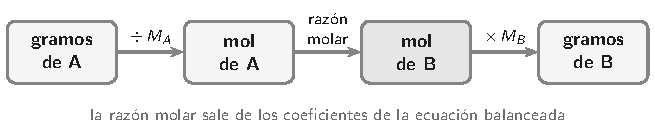
\includegraphics[max width=0.92\linewidth,max height=8.5cm]{qui/reac_camino}
\end{center}
 

\textbf{Ejemplo.} C\textsubscript{3}H\textsubscript{8} + 5 O\textsubscript{2} \ensuremath{\rightarrow} 3 CO\textsubscript{2} + 4 H\textsubscript{2}O. ¿Qué masa de CO\textsubscript{2} se forma al quemar 22 g de propano? (C = 12, H = 1, O = 16)

 

\textbf{Paso 1. Gramos a mol.} $M(\text{C}_3\text{H}_8) = 44$ g/mol: $n = \dfrac{22}{44} = 0{,}5$ mol.

 

\textbf{Paso 2. Razón molar.} 1 mol de propano da 3 mol de CO\textsubscript{2}: $0{,}5\cdot 3 = 1{,}5$ mol.

 

\textbf{Paso 3. Mol a gramos.} $m = 1{,}5\cdot 44 = 66$ g de CO\textsubscript{2}.

  
\begin{ejemplo}[{Ejemplo resuelto}] Fe + S \ensuremath{\rightarrow} FeS. ¿Qué masa máxima de FeS se forma con 112 g de Fe (56 g/mol) y exceso de S (32 g/mol)?\par \textbf{Paso 1.} $n(\text{Fe}) = \dfrac{112}{56} = 2$ mol.\par \textbf{Paso 2.} Razón 1 : 1: se forman 2 mol de FeS.\par \textbf{Paso 3.} $M(\text{FeS}) = 88$ g/mol: $2\cdot 88 = 176$ g.\par \textbf{Comprobación:} reaccionan 112 g de Fe y $2\cdot 32 = 64$ g de S: $112 + 64 = 176$ g. \ding{52}\end{ejemplo}
 
\begin{ojo}[{Error típico}] Saltarse los mol y aplicar la razón molar a los gramos: «1 : 3, entonces 22 g de propano dan 66 g de CO\textsubscript{2}» acierta aquí de casualidad, porque las dos masas molares son 44. En general falla.\end{ojo}
\subsection{Reactivo limitante y reactivo en exceso}
Para hacer un sándwich necesitas 2 panes y 1 lámina de queso. Si tienes 10 panes y 3 láminas, solo haces 3 sándwiches y sobran 4 panes: el queso \textbf{limita}.

 

En una reacción pasa lo mismo. El \textbf{reactivo limitante} es el que se acaba primero y decide cuánto producto se forma. El otro es el \textbf{reactivo en exceso}: parte de él sobra.

 
\begin{center}
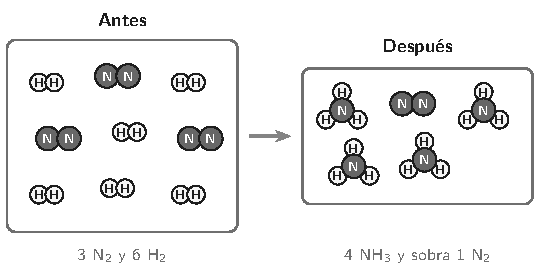
\includegraphics[max width=0.92\linewidth,max height=8.5cm]{qui/reac_limitante}
\end{center}
 

N\textsubscript{2} + 3 H\textsubscript{2} \ensuremath{\rightarrow} 2 NH\textsubscript{3}. Con 3 N\textsubscript{2} y 6 H\textsubscript{2}: los 6 H\textsubscript{2} alcanzan para 2 N\textsubscript{2}, y forman 4 NH\textsubscript{3}. Sobra 1 N\textsubscript{2}. El H\textsubscript{2} es el limitante, aunque haya más moléculas de H\textsubscript{2} que de N\textsubscript{2}.

  
\begin{clave}[{Método del cociente}] 1. Pasa cada reactivo a mol. 2. Divide los mol de cada uno por su coeficiente. 3. El \textbf{menor cociente} es el limitante. 4. Calcula el producto con el limitante.\par En el ejemplo: N\textsubscript{2}: $\dfrac{3}{1} = 3$; H\textsubscript{2}: $\dfrac{6}{3} = 2$. El menor es el del H\textsubscript{2}.\end{clave}
 
\begin{ojo}[{Error típico}] Elegir como limitante el reactivo del que hay menos mol o menos gramos. Lo que importa es cuánto hay \textbf{comparado con cuánto se necesita}: por eso se divide por el coeficiente.\end{ojo}
 
\begin{ojo}[{Otro error}] Calcular el producto con el reactivo en exceso. Da una cantidad mayor que la real, porque el limitante se acaba antes.\end{ojo}
\subsection{La tabla inicial -- reacciona -- final}
Una tabla ordena todo el cálculo y muestra cuánto sobra. Ejemplo: CH\textsubscript{4} + 2 O\textsubscript{2} \ensuremath{\rightarrow} CO\textsubscript{2} + 2 H\textsubscript{2}O, con 16 g de CH\textsubscript{4} (1 mol) y 96 g de O\textsubscript{2} (3 mol).

 

\textbf{Paso 1. Limitante.} CH\textsubscript{4}: $\dfrac{1}{1} = 1$; O\textsubscript{2}: $\dfrac{3}{2} = 1{,}5$. El limitante es el CH\textsubscript{4}.

 

\textbf{Paso 2. Tabla (en mol).} Lo que reacciona sale de la razón molar con el limitante.

 
\begin{center}\small
\begin{tabular}{@{}lllll@{}}
\toprule
 & \textbf{CH\textsubscript{4}} & \textbf{O\textsubscript{2}} & \textbf{CO\textsubscript{2}} & \textbf{H\textsubscript{2}O} \\
\midrule
Inicial & 1 & 3 & 0 & 0 \\
Reacciona / se forma & \ensuremath{-}1 & \ensuremath{-}2 & +1 & +2 \\
Final & 0 & 1 & 1 & 2 \\
\bottomrule
\end{tabular}
\end{center}
 

\textbf{Paso 3. Lee el resultado.} Se forman 1 mol de CO\textsubscript{2} (44 g) y 2 mol de H\textsubscript{2}O (36 g). Sobra 1 mol de O\textsubscript{2} (32 g).

  
\begin{clave}[{Comprobación con Lavoisier}] Masa inicial: $16 + 96 = 112$ g. Masa final: $32 + 44 + 36 = 112$ g. \ding{52} La masa de lo que sobra se cuenta en el final.\end{clave}
 
\begin{clave}[{Tablas de ensayos}] En la PAES aparecen tablas con varios ensayos: uno de los reactivos se mantiene fijo y el otro aumenta. Mientras el producto crece al aumentar un reactivo, ese reactivo es el limitante. Cuando el producto deja de crecer, el limitante pasó a ser el otro.\end{clave}
 
\begin{ojo}[{Ojo}] El reactivo limitante queda en 0 al final. Si en tu tabla un reactivo termina negativo, elegiste mal el limitante.\end{ojo}
\subsection{Lo clave del tema}
\begin{center}\small
\begin{tabularx}{\linewidth}{@{}>{\raggedright\arraybackslash\hsize=0.92\hsize}X>{\raggedright\arraybackslash\hsize=1.08\hsize}X@{}}
\toprule
\textbf{Situación} & \textbf{Qué hacer} \\
\midrule
Tengo mol, busco mol & multiplico por $\dfrac{\text{coef. de lo que busco}}{\text{coef. de lo que tengo}}$ \\
Tengo gramos, busco gramos & g \ensuremath{\rightarrow} mol (÷ $M$) \ensuremath{\rightarrow} razón molar \ensuremath{\rightarrow} mol \ensuremath{\rightarrow} g (× $M$) \\
Me dan cantidades de dos reactivos & busco el limitante: menor cociente mol / coeficiente \\
Preguntan cuánto sobra & inicial \ensuremath{-} lo que reaccionó con el limitante \\
\bottomrule
\end{tabularx}
\end{center}
 
\begin{clave}[{Recuerda}] · La razón molar es en mol: 2 H\textsubscript{2} + O\textsubscript{2} son 2 mol de H\textsubscript{2} (4 g) con 1 mol de O\textsubscript{2} (32 g).\par · En N\textsubscript{2}O\textsubscript{5} + H\textsubscript{2}O \ensuremath{\rightarrow} 2 HNO\textsubscript{3}, formar 4 mol de HNO\textsubscript{3} requiere $4\cdot\dfrac{1}{2} = 2$ mol de N\textsubscript{2}O\textsubscript{5}.\par · El limitante se elige dividiendo por los coeficientes: en N\textsubscript{2} + 3 H\textsubscript{2}, con 3 mol de N\textsubscript{2} y 6 mol de H\textsubscript{2}, $\dfrac{6}{3} = 2 < \dfrac{3}{1} = 3$: limita el H\textsubscript{2}.\par · El producto siempre se calcula con el reactivo limitante.\par · La masa de producto es solo lo que reaccionó; lo que sobra no es producto.\end{clave}
 
\begin{clave}[{Método PAES}] 1. Revisa que la ecuación esté balanceada. 2. Pasa todos los datos a mol. 3. Si hay dos reactivos, divide por los coeficientes y elige el limitante. 4. Usa la razón molar con el limitante. 5. Vuelve a gramos si te los piden. 6. Comprueba con la conservación de la masa.\end{clave}
\begin{elejemplo}{PAES Regular 2026, adaptada}
Una profesora escribe la siguiente ecuación balanceada, que representa la reacción entre aluminio y cloro para formar cloruro de aluminio:

\begin{center}
2 Al (s) + 3 Cl\textsubscript{2} (g) \ensuremath{\rightarrow} 2 AlCl\textsubscript{3} (s)
\end{center}

De acuerdo con la ecuación, ¿cuál es la máxima cantidad de AlCl\textsubscript{3} que se forma a partir de 27 g de Al y 213 g de Cl\textsubscript{2}?

Masas atómicas (g/mol): Al = 27; Cl = 35,5.
\alts{0,5 mol}{1,0 mol}{2,0 mol}{4,0 mol}
\solucion{\textbf{Paso 1. ¿Qué nos piden?} La cantidad máxima de producto. Nos dan cantidades de los dos reactivos, así que primero hay que ver cuál se acaba antes: el reactivo limitante.

\textbf{Paso 2. Pasa a mol.} Al: $n = \dfrac{27}{27} = 1$ mol. Cl\textsubscript{2}: $M = 2\cdot 35{,}5 = 71$ g/mol, así que $n = \dfrac{213}{71} = 3$ mol.

\textbf{Paso 3. Divide por los coeficientes.} Al: $\dfrac{1}{2} = 0{,}5$. Cl\textsubscript{2}: $\dfrac{3}{3} = 1$. El menor cociente es el del Al: el aluminio es el reactivo limitante.

\textbf{Paso 4. Producto con el limitante.} 2 mol de Al forman 2 mol de AlCl\textsubscript{3} (razón 1 : 1). Con 1 mol de Al se forma 1 mol de AlCl\textsubscript{3}.

\textbf{Paso 5. Tabla (en mol).}

\begin{center}\small
\begin{tabular}{@{}llll@{}}
\toprule
 & \textbf{Al} & \textbf{Cl\textsubscript{2}} & \textbf{AlCl\textsubscript{3}} \\
\midrule
Inicial & 1 & 3 & 0 \\
Reacciona / se forma & \ensuremath{-}1 & $-1\cdot\dfrac{3}{2} = -1{,}5$ & +1 \\
Final & 0 & 1,5 & 1 \\
\bottomrule
\end{tabular}
\end{center}

\textbf{Respuesta:} 1,0 mol de AlCl\textsubscript{3}.

\textbf{Comprobación:} con Lavoisier. Masa inicial: $27 + 213 = 240$ g. Masa final: AlCl\textsubscript{3}, $1\cdot(27 + 3\cdot 35{,}5) = 133{,}5$ g, más el Cl\textsubscript{2} que sobra, $1{,}5\cdot 71 = 106{,}5$ g. Total: $133{,}5 + 106{,}5 = 240$ g. \ding{52}

\textbf{¿Por qué no las otras?} 0,5 mol es el cociente del Al ($\dfrac{1}{2}$), que solo sirve para comparar; no es la cantidad de producto. 2,0 mol se calcula con el Cl\textsubscript{2}, el reactivo en exceso ($3\cdot\dfrac{2}{3} = 2$): para eso harían falta 2 mol de Al y solo hay 1. 4,0 mol suma los mol de los reactivos ($1 + 3$), y los mol no se conservan en una reacción.

\textbf{\color{cienciaD}Para recordar.} Con dos reactivos, divide sus mol por los coeficientes: el menor manda y con él se calcula el producto.}{B}
\end{elejemplo}

%% =====================================================================
%% qui_composicion
\section[Composición porcentual y fórmulas empírica y molecular]{Composición porcentual y fórmulas empírica y molecular}
\modcomun\ \ {\color{gris}\itshape Calcular el porcentaje en masa de cada elemento de un compuesto, la masa de un elemento en una muestra, y obtener la fórmula empírica y la molecular a partir de porcentajes o de masas.\par}
\subsection{Composición porcentual}
La \textbf{composición porcentual} de un compuesto dice qué porcentaje de su masa corresponde a cada elemento. Se calcula con la masa de un mol:

 
\begin{center}
$\%\,\text{elemento} = \dfrac{\text{masa del elemento en 1 mol}}{M\ \text{del compuesto}}\cdot 100$
\end{center}
 

\textbf{Ejemplo: agua, H\textsubscript{2}O} ($M = 18$ g/mol). En 1 mol hay $2\cdot 1 = 2$ g de H y 16 g de O.

 

$\%\,\text{H} = \dfrac{2}{18}\cdot 100 \approx 11{,}1\%$ y $\%\,\text{O} = \dfrac{16}{18}\cdot 100 \approx 88{,}9\%$.

 
\begin{center}\small
\begin{tabular}{@{}lll@{}}
\toprule
\textbf{Compuesto} & \textbf{$M$ (g/mol)} & \textbf{Composición} \\
\midrule
MgO & 40 & Mg $\dfrac{24}{40} = 60\%$ · O $40\%$ \\
CaCO\textsubscript{3} & 100 & Ca 40 \% · C 12 \% · O 48 \% \\
SO\textsubscript{3} & 80 & S $\dfrac{32}{80} = 40\%$ · O 60 \% \\
\bottomrule
\end{tabular}
\end{center}
  
\begin{clave}[{Siempre suman 100 \%}] Si conoces todos los porcentajes menos uno, el que falta es 100 menos la suma de los otros. Te sirve para comprobar o para hallar el oxígeno «por diferencia».\end{clave}
 
\begin{clave}[{No depende de la muestra}] Por la ley de Proust, el porcentaje es el mismo en 1 g o en 1 tonelada del compuesto puro. Una muestra de 10 g de MgO y otra de 25 g tienen ambas 60 \% de Mg; lo que cambia es la \textbf{masa} de Mg (6 g y 15 g).\end{clave}
 
\begin{ojo}[{Error típico}] Olvidar el subíndice. En H\textsubscript{2}O la masa de H en un mol es $2\cdot 1 = 2$ g, no 1 g. En CaCO\textsubscript{3} la masa de O es $3\cdot 16 = 48$ g.\end{ojo}
\subsection{Masa de un elemento en una muestra y comparar porcentajes}
\textbf{Masa de un elemento en una muestra.} Se multiplica la masa de la muestra por la fracción del elemento.

 
\begin{ejemplo}[{Ejemplo resuelto}] ¿Qué masa de oxígeno hay en 80 g de SO\textsubscript{3}? (S = 32, O = 16)\par \textbf{Paso 1.} $M(\text{SO}_3) = 32 + 48 = 80$ g/mol. En 80 g hay 48 g de O.\par \textbf{Paso 2.} La muestra pesa justo 80 g (1 mol): tiene \textbf{48 g} de O.\par Si la muestra fuera de 200 g: $200\cdot\dfrac{48}{80} = 200\cdot 0{,}6 = 120$ g de O.\end{ejemplo}
 

\textbf{Otro camino:} pasa la muestra a mol y multiplica por los átomos del elemento. 200 g de SO\textsubscript{3} son $\dfrac{200}{80} = 2{,}5$ mol; tienen $2{,}5\cdot 3 = 7{,}5$ mol de O, o sea $7{,}5\cdot 16 = 120$ g. \ding{52}

  

\textbf{Comparar porcentajes sin calculadora.} Para saber qué compuesto tiene mayor porcentaje de un elemento, mira cuánta masa de «lo demás» acompaña a cada átomo de ese elemento: mientras menos lo acompañe, mayor su porcentaje.

 
\begin{center}\small
\begin{tabular}{@{}lll@{}}
\toprule
\textbf{Óxido} & \textbf{O por cada N} & \textbf{\% de N} \\
\midrule
N\textsubscript{2}O & 0,5 & 63,6 \% \\
NO & 1 & 46,7 \% \\
N\textsubscript{2}O\textsubscript{3} & 1,5 & 36,8 \% \\
NO\textsubscript{2} & 2 & 30,4 \% \\
N\textsubscript{2}O\textsubscript{5} & 2,5 & 25,9 \% \\
\bottomrule
\end{tabular}
\end{center}
 
\begin{ojo}[{Error típico}] Creer que el compuesto con más átomos de N en la fórmula tiene más porcentaje de N. N\textsubscript{2}O\textsubscript{5} tiene 2 N, pero es el de menor porcentaje: cada N viene con 2,5 O.\end{ojo}
\subsection{Fórmula molecular, empírica y estructural}
\begin{center}
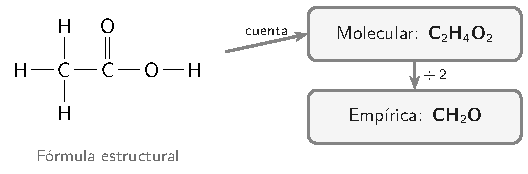
\includegraphics[max width=0.92\linewidth,max height=8.5cm]{qui/reac_formulas}
\end{center}
 
\begin{center}\small
\begin{tabularx}{\linewidth}{@{}>{\raggedright\arraybackslash\hsize=0.52\hsize}X>{\raggedright\arraybackslash\hsize=1.48\hsize}X@{}}
\toprule
\textbf{Fórmula} & \textbf{Qué muestra} \\
\midrule
Estructural & cómo están unidos los átomos \\
Molecular & cuántos átomos de cada elemento hay en \textbf{una molécula} \\
Empírica & la proporción \textbf{más simple} de números enteros entre los átomos \\
\bottomrule
\end{tabularx}
\end{center}
  
\begin{center}\small
\begin{tabular}{@{}lll@{}}
\toprule
\textbf{Sustancia} & \textbf{Molecular} & \textbf{Empírica} \\
\midrule
glucosa & C\textsubscript{6}H\textsubscript{12}O\textsubscript{6} & CH\textsubscript{2}O \\
benceno & C\textsubscript{6}H\textsubscript{6} & CH \\
agua oxigenada & H\textsubscript{2}O\textsubscript{2} & HO \\
eteno & C\textsubscript{2}H\textsubscript{4} & CH\textsubscript{2} \\
agua & H\textsubscript{2}O & H\textsubscript{2}O (ya es la más simple) \\
\bottomrule
\end{tabular}
\end{center}
 
\begin{clave}[{Cómo se obtiene la empírica}] Divide todos los subíndices de la molecular por su máximo común divisor. Si no se pueden dividir, la empírica es igual a la molecular.\end{clave}
 
\begin{ojo}[{Contar desde una estructura}] Cuenta los H de cada carbono y también los de los grupos OH, NH\textsubscript{2} o COOH. Olvidar el H del OH es el error más común. Además, varias sustancias pueden tener la misma empírica: CH\textsubscript{2}O es la de la glucosa, del ácido acético y del metanal.\end{ojo}
\subsection{Fórmula empírica a partir de porcentajes o masas}
\textbf{Los pasos:}

 

\textbf{1. Gramos.} Si te dan porcentajes, supón 100 g de compuesto: cada porcentaje pasa a ser gramos.

 

\textbf{2. Mol.} Divide los gramos de cada elemento por su masa atómica.

 

\textbf{3. Divide por el menor.} Divide todos los resultados por el más pequeño.

 

\textbf{4. Enteros.} Si sale algo como 1,5 multiplica todo por 2; si sale 1,33 o 1,67, por 3; si sale 1,25, por 4.

 
\begin{ejemplo}[{Ejemplo resuelto}] Un óxido de hierro tiene 70 \% de Fe y 30 \% de O (Fe = 56, O = 16).\par \textbf{1.} En 100 g: 70 g de Fe y 30 g de O.\par \textbf{2.} Fe: $\dfrac{70}{56} = 1{,}25$ mol. O: $\dfrac{30}{16} = 1{,}875$ mol.\par \textbf{3.} Dividimos por 1,25: Fe 1 y O 1,5.\par \textbf{4.} Multiplicamos por 2: Fe 2 y O 3. Fórmula empírica: \textbf{Fe\textsubscript{2}O\textsubscript{3}}.\end{ejemplo}
  
\begin{clave}[{Desde masas}] Si te dan masas de cada elemento, salta el paso 1. Ejemplo: un compuesto tiene 14 g de N y 24 g de O. N: $\dfrac{14}{14} = 1$ mol. O: $\dfrac{24}{16} = 1{,}5$ mol. Razón 1 : 1,5 = 2 : 3: \textbf{N\textsubscript{2}O\textsubscript{3}}.\end{clave}
 
\begin{ojo}[{Error típico}] Usar los porcentajes o las masas como subíndices, sin dividir por la masa atómica: 70 \% Fe y 30 \% O \textbf{no} es Fe\textsubscript{7}O\textsubscript{3}. Los subíndices cuentan átomos (mol), no gramos.\end{ojo}
 
\begin{ojo}[{Otro error}] Redondear 1,5 a 1 o a 2. Solo se redondea lo que está muy cerca de un entero (1,98 \ensuremath{\rightarrow} 2); 1,5 obliga a multiplicar.\end{ojo}
\subsection{De la fórmula empírica a la molecular}
La fórmula molecular es la empírica multiplicada por un número entero $n$. Para hallar $n$ se necesita la masa molar del compuesto:

 
\begin{center}
$n = \dfrac{M\ \text{del compuesto}}{M\ \text{de la fórmula empírica}}$
\end{center}
 
\begin{ejemplo}[{Ejemplo resuelto}] Un compuesto tiene 40 \% de C, 6,7 \% de H y 53,3 \% de O, y su masa molar es 180 g/mol.\par \textbf{1.} En 100 g: C $\dfrac{40}{12}\approx 3{,}33$ mol; H $\dfrac{6{,}7}{1} = 6{,}7$ mol; O $\dfrac{53{,}3}{16}\approx 3{,}33$ mol.\par \textbf{2.} Dividimos por 3,33: C 1, H 2, O 1. Empírica: CH\textsubscript{2}O, con $M = 12 + 2 + 16 = 30$ g/mol.\par \textbf{3.} $n = \dfrac{180}{30} = 6$. Molecular: C\textsubscript{6}H\textsubscript{12}O\textsubscript{6} (glucosa).\end{ejemplo}
  
\begin{clave}[{¿Cómo se miden esos porcentajes?}] En el laboratorio se quema una masa conocida del compuesto y se masan el CO\textsubscript{2} y el H\textsubscript{2}O que se forman. De ahí se calculan las masas de C y de H de la muestra; el O se obtiene por diferencia. Con esas masas se calcula la fórmula empírica. En la PAES este procedimiento puede aparecer como pregunta de habilidades.\end{clave}
 
\begin{ojo}[{Error típico}] Multiplicar solo un elemento por $n$. Se multiplican \textbf{todos} los subíndices: (CH\textsubscript{2}O)\textsubscript{6} = C\textsubscript{6}H\textsubscript{12}O\textsubscript{6}.\end{ojo}
 
\begin{clave}[{Control}] La masa molar de la fórmula molecular debe dar exactamente la del enunciado: $6\cdot 12 + 12\cdot 1 + 6\cdot 16 = 180$. \ding{52}\end{clave}
\subsection{Lo clave del tema}
\begin{center}\small
\begin{tabularx}{\linewidth}{@{}>{\raggedright\arraybackslash\hsize=0.93\hsize}X>{\raggedright\arraybackslash\hsize=1.07\hsize}X@{}}
\toprule
\textbf{Me piden} & \textbf{Hago} \\
\midrule
\% de un elemento & $\dfrac{\text{subíndice}\cdot\text{masa atómica}}{M}\cdot 100$ \\
masa de un elemento en una muestra & masa de la muestra $\cdot\ \dfrac{\text{masa del elemento en 1 mol}}{M}$ \\
fórmula empírica desde \% o masas & gramos \ensuremath{\rightarrow} mol (÷ masa atómica) \ensuremath{\rightarrow} ÷ el menor \ensuremath{\rightarrow} enteros \\
fórmula molecular & $n = \dfrac{M}{M_{\text{empírica}}}$ y multiplico todos los subíndices \\
fórmula empírica desde la molecular & divido los subíndices por su máximo común divisor \\
\bottomrule
\end{tabularx}
\end{center}
 
\begin{clave}[{Recuerda}] · Los porcentajes se pasan a moles: C $\dfrac{80}{12}$, H $\dfrac{20}{1}$, razón 1 : 3, fórmula CH\textsubscript{3}.\par · \% H en H\textsubscript{2}O $= \dfrac{2}{18}\approx 11{,}1\%$: cuenta el subíndice.\par · Una razón 1 : 1,5 se multiplica por 2: Fe\textsubscript{2}O\textsubscript{3}.\par · El ácido butanoico es C\textsubscript{4}H\textsubscript{8}O\textsubscript{2} (incluye el H del OH).\par · La composición porcentual no depende de la muestra: cambia la masa de Mg, no su \%.\end{clave}
 
\begin{clave}[{Método PAES}] 1. Calcula la masa molar con cuidado. 2. Para porcentajes, divide la masa del elemento en un mol por $M$; para comparar, mira cuánto acompaña a cada átomo del elemento. 3. Para fórmulas, trabaja siempre en mol: divide por la masa atómica, luego por el menor, y lleva a enteros. 4. Comprueba: los porcentajes suman 100 y la masa molar de tu fórmula coincide con la del enunciado.\end{clave}
\begin{elejemplo}{PAES Invierno 2026, adaptada}
En una actividad sobre la composición de los óxidos de nitrógeno, una profesora presenta la siguiente información sobre cuatro compuestos formados solo por nitrógeno y oxígeno:

¿Cuál de los compuestos tiene la fórmula empírica N\textsubscript{2}O\textsubscript{3}?

Masas atómicas (g/mol): N = 14; O = 16.
\begin{center}\small
\begin{tabular}{@{}lll@{}}
\toprule
\textbf{Compuesto} & \textbf{Masa de N (g)} & \textbf{Masa de O (g)} \\
\midrule
\textbf{1} & 7 & 8 \\
\textbf{2} & 14 & 24 \\
\textbf{3} & 28 & 16 \\
\textbf{4} & 14 & 40 \\
\bottomrule
\end{tabular}
\end{center}
\alts{El compuesto 1.}{El compuesto 2.}{El compuesto 3.}{El compuesto 4.}
\solucion{\textbf{Paso 1. ¿Qué nos piden?} El compuesto cuya proporción de átomos es N : O = 2 : 3. Las masas no se comparan directamente: hay que pasarlas a mol, porque los subíndices cuentan átomos.

\textbf{Paso 2. Qué buscamos.} En N\textsubscript{2}O\textsubscript{3} hay 1,5 átomos de O por cada átomo de N. Buscamos el compuesto con razón $\dfrac{n_{\text{O}}}{n_{\text{N}}} = 1{,}5$.

\textbf{Paso 3. Compuesto 1.} N: $\dfrac{7}{14} = 0{,}5$ mol. O: $\dfrac{8}{16} = 0{,}5$ mol. Razón 1 : 1, fórmula empírica NO.

\textbf{Paso 4. Compuesto 2.} N: $\dfrac{14}{14} = 1$ mol. O: $\dfrac{24}{16} = 1{,}5$ mol. Razón 1 : 1,5; multiplicando por 2, 2 : 3. Fórmula empírica \textbf{N\textsubscript{2}O\textsubscript{3}}.

\textbf{Paso 5. Revisa los otros.} Compuesto 3: N $\dfrac{28}{14} = 2$, O $\dfrac{16}{16} = 1$: N\textsubscript{2}O. Compuesto 4: N 1, O $\dfrac{40}{16} = 2{,}5$: razón 2 : 5, N\textsubscript{2}O\textsubscript{5}.

\textbf{Respuesta:} el compuesto 2.

\textbf{Comprobación:} en N\textsubscript{2}O\textsubscript{3} hay $2\cdot 14 = 28$ g de N por cada $3\cdot 16 = 48$ g de O. Razón en masa $28 : 48 = 14 : 24$, justo la del compuesto 2. \ding{52}

\textbf{¿Por qué no las otras?} El compuesto 1 tiene masas parecidas (7 y 8), lo que puede hacer pensar en «casi 1 : 1 en masa», pero en mol es NO. El compuesto 3 tiene el doble de N que de O en mol: es N\textsubscript{2}O; quien lo elige compara los gramos (28 y 16) sin dividir por la masa atómica. El compuesto 4 es N\textsubscript{2}O\textsubscript{5}: tiene 2,5 O por cada N, más de lo necesario.

\textbf{\color{cienciaD}Para recordar.} Para la fórmula empírica, divide cada masa por su masa atómica y compara los mol, nunca los gramos.}{B}
\end{elejemplo}

\chapter{Soluciones químicas}
%% =====================================================================
%% qui_soluciones
\section[Características de las soluciones y solubilidad]{Características de las soluciones y solubilidad}
\modcomun\ \ {\color{gris}\itshape Soluto y solvente, propiedades de las soluciones, soluciones insaturadas, saturadas y sobresaturadas, solubilidad y los factores que la cambian, y cómo leer una curva de solubilidad.\par}
\subsection{¿Qué es una solución?}
Una \textbf{solución} (o disolución) es una \textbf{mezcla homogénea}: a simple vista, e incluso con microscopio, se ve una sola fase. Tiene dos tipos de componentes:

 
\begin{itemize}
  \item \textbf{Soluto}: lo que se disuelve. Por lo general está en menor cantidad, y puede haber más de uno.
  \item \textbf{Solvente} (o disolvente): lo que disuelve. Está en mayor cantidad y define el estado de la solución. El agua es el solvente más común, por eso se le llama \textbf{solvente universal}; las soluciones en agua se llaman \textbf{acuosas}.
\end{itemize}
 

Las masas se suman: \textbf{masa de solución = masa de soluto + masa de solvente}. Si disuelves 10 g de sal en 90 g de agua, obtienes 100 g de solución. Los volúmenes, en cambio, no siempre se suman exactamente (50 mL de etanol con 50 mL de agua dan unos 97 mL). Por eso los problemas dicen "considere volúmenes aditivos" cuando quieren que los sumes.

 
\begin{center}
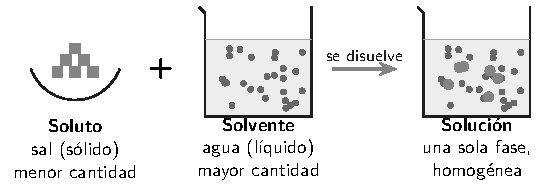
\includegraphics[max width=0.92\linewidth,max height=8.5cm]{qui/sol_particulas}
\end{center}
  
\begin{clave}[{Soluciones en los tres estados}] \begin{center}\small
\begin{tabularx}{\linewidth}{@{}>{\raggedright\arraybackslash\hsize=0.48\hsize}X>{\raggedright\arraybackslash\hsize=0.78\hsize}X>{\raggedright\arraybackslash\hsize=1.74\hsize}X@{}}
\toprule
\textbf{Solución} & \textbf{Soluto en solvente} & \textbf{Ejemplo} \\
\midrule
Gaseosa & gas en gas & aire (O\textsubscript{2}, Ar y CO\textsubscript{2} en N\textsubscript{2}) \\
Líquida & sólido en líquido & agua de mar, suero fisiológico \\
Líquida & gas en líquido & bebida gaseosa (CO\textsubscript{2} en agua) \\
Líquida & líquido en líquido & vinagre (ácido acético en agua), vino \\
Sólida & sólido en sólido & bronce (estaño en cobre), acero (carbono en hierro) \\
\bottomrule
\end{tabularx}
\end{center}\end{clave}
 
\begin{ojo}[{¿Quién es el solvente?}] El que define el estado de la solución y, casi siempre, el que está en mayor cantidad. En el aire es el nitrógeno (78 \%). En una bebida con mucha azúcar, el solvente sigue siendo el agua.\end{ojo}
\subsection{Propiedades de las soluciones}
Una solución verdadera cumple con todo esto:

 
\begin{itemize}
  \item \textbf{Una sola fase}: es homogénea; cualquier gota tiene la misma composición.
  \item \textbf{Es transparente}, aunque puede tener color (el sulfato de cobre(II) en agua es azul).
  \item \textbf{El soluto no sedimenta}: aunque la dejes reposar días, no se va al fondo.
  \item \textbf{No se separa por filtración}: el soluto atraviesa el papel filtro. Sí se separa con métodos que cambian de estado, como la \textbf{evaporación} (queda el sólido) o la \textbf{destilación}.
  \item \textbf{Composición variable}: puedes poner más o menos soluto (hasta un límite) y sigue siendo solución. Un compuesto, en cambio, tiene composición fija.
  \item \textbf{Conduce la corriente} solo si el soluto es un \textbf{electrolito} (sales como NaCl, ácidos, bases), que libera iones. Si el soluto es molecular, como el azúcar o el etanol, no conduce.
\end{itemize}
  
\begin{ejemplo}[{Ejemplo: agua con sal y agua con arena}] \begin{center}\small
\begin{tabularx}{\linewidth}{@{}>{\raggedright\arraybackslash\hsize=0.88\hsize}X>{\raggedright\arraybackslash\hsize=0.80\hsize}X>{\raggedright\arraybackslash\hsize=1.32\hsize}X@{}}
\toprule
\textbf{Propiedad} & \textbf{Agua con sal} & \textbf{Agua con arena} \\
\midrule
Fases & 1 & 2 \\
¿Sedimenta al reposar? & No & Sí \\
¿Se separa al filtrar? & No & Sí \\
¿Conduce la corriente? & Sí (iones Na\textsuperscript{+} y Cl\textsuperscript{\ensuremath{-}}) & No (como el agua pura, casi nada) \\
Tipo de mezcla & Solución & Mezcla heterogénea \\
\bottomrule
\end{tabularx}
\end{center}\end{ejemplo}
 
\begin{ojo}[{Disolver no es reaccionar}] Cuando el azúcar se disuelve, sus moléculas se separan y se rodean de agua, pero siguen siendo azúcar: es un cambio físico. Si evaporas el agua, recuperas el azúcar.\end{ojo}
\subsection{Insaturada, saturada y sobresaturada}
\textbf{1. Diluida o concentrada.} Es una comparación entre soluciones: un jugo con poco polvo está \textbf{diluido} y uno con mucho, \textbf{concentrado}. Son términos relativos: no dicen si cabe más soluto.

 

\textbf{2. Según la solubilidad.} Cada soluto tiene un máximo que se disuelve en cierta cantidad de solvente a una temperatura: su \textbf{solubilidad}. Comparando con ese máximo:

 
\begin{itemize}
  \item \textbf{Insaturada}: tiene menos soluto que el máximo. Si agregas más, se disuelve.
  \item \textbf{Saturada}: tiene justo el máximo. Si agregas más, queda sin disolver en el fondo, y la solución sigue saturada.
  \item \textbf{Sobresaturada}: tiene disuelto más que el máximo. Se logra disolviendo en caliente y enfriando sin mover el recipiente. Es \textbf{inestable}: un golpe o un cristal "semilla" hace que el exceso precipite de golpe, y queda saturada.
\end{itemize}
 
\begin{center}
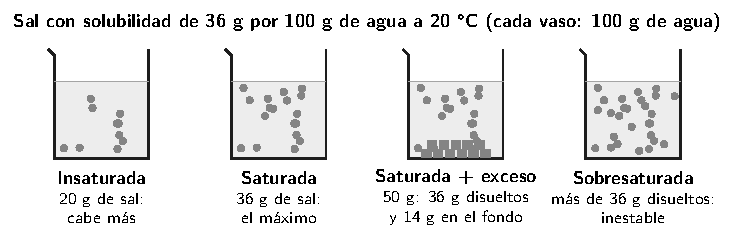
\includegraphics[max width=0.92\linewidth,max height=8.5cm]{qui/sol_clasificacion}
\end{center}
  
\begin{ejemplo}[{Ejemplo resuelto}] La solubilidad de una sal es 36 g por 100 g de agua a 20 °C. ¿Qué pasa si agregas 50 g de sal a 200 g de agua a 20 °C?\par \textbf{Paso 1.} Escala el máximo a la masa de agua: 200 g de agua disuelven $2\cdot 36 = 72$ g.\par \textbf{Paso 2.} Compara: $50 < 72$, así que se disuelve todo. La solución es \textbf{insaturada} y todavía caben $72 - 50 = 22$ g.\par \textbf{Paso 3.} ¿Y si los 50 g van en solo 100 g de agua? Se disuelven 36 g y quedan $50 - 36 = 14$ g en el fondo: \textbf{saturada} con exceso.\end{ejemplo}
 
\begin{ojo}[{Sobresaturada no es "con sal en el fondo"}] Si queda sólido en el fondo, la solución está \textbf{saturada}. Sobresaturada es tener disuelto más que el máximo, sin sólido, y es inestable.\end{ojo}
\subsection{La solubilidad y sus factores}
La \textbf{solubilidad} es la máxima cantidad de soluto que se disuelve en una cantidad dada de solvente a cierta temperatura (y presión). Se suele dar en \textbf{g de soluto por 100 g de agua}. Depende de tres factores:

 

\textbf{1. Naturaleza del soluto y del solvente.} "Lo semejante disuelve a lo semejante": las sustancias \textbf{polares} o iónicas se disuelven en solventes polares, como el agua; las \textbf{apolares}, en solventes apolares. La sal y el azúcar se disuelven en agua; el aceite no, y forma dos fases. El yodo (apolar) casi no se disuelve en agua, pero sí en hexano.

 

\textbf{2. Temperatura.} En la mayoría de los sólidos, la solubilidad \textbf{aumenta} al subir la temperatura (algunas sales, como el carbonato de litio, hacen lo contrario). En los \textbf{gases} siempre \textbf{disminuye}: el agua tibia retiene menos gas. Por eso una bebida tibia pierde el gas más rápido y un río con agua tibia tiene menos oxígeno para los peces.

 

\textbf{3. Presión.} Afecta casi solo a los \textbf{gases}: a mayor presión del gas sobre el líquido, más gas se disuelve (ley de Henry). La bebida se embotella con CO\textsubscript{2} a alta presión; al abrirla, la presión baja y el gas escapa en burbujas.

  
\begin{center}
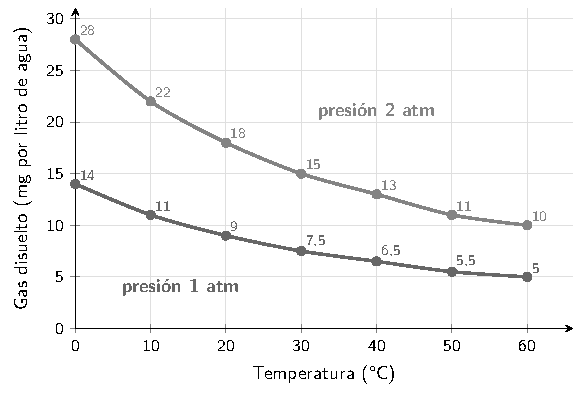
\includegraphics[max width=0.92\linewidth,max height=8.5cm]{qui/sol_gas}
\end{center}
 

Datos inventados para un gas cualquiera, con la forma real: al calentar baja la solubilidad, y al duplicar la presión se duplica.

 
\begin{ojo}[{Solubilidad no es rapidez}] Agitar o moler el soluto hace que se disuelva \textbf{más rápido}, pero no cambia \textbf{cuánto} se disuelve como máximo. De los factores de la vida diaria, solo la temperatura (y, en gases, la presión) cambia la solubilidad.\end{ojo}
 
\begin{clave}[{Pistas en un ensayo de solubilidad}] Dos líquidos que se mezclan en una sola fase son del mismo tipo (los dos polares o los dos apolares). Si forman dos fases, son de distinto tipo; arriba queda el menos denso.\end{clave}
\subsection{Curvas de solubilidad}
\begin{center}
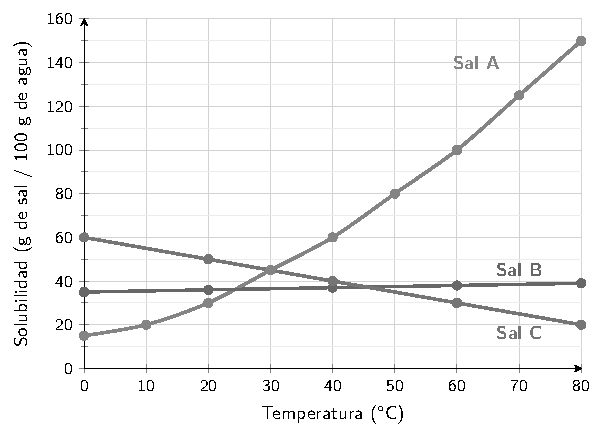
\includegraphics[max width=0.92\linewidth,max height=8.5cm]{qui/sol_curvas}
\end{center}
 

Una \textbf{curva de solubilidad} muestra la solubilidad de una sustancia (eje vertical) a cada temperatura (eje horizontal). El gráfico tiene datos inventados para tres sales: la A se comporta como el nitrato de potasio (sube mucho al calentar), la B como el cloruro de sodio (casi no cambia) y la C como el carbonato de litio (baja al calentar).

 

\textbf{Cómo leerla.} Sube desde la temperatura hasta la curva y lee a la izquierda: la sal A a 40 °C tiene una solubilidad de 60 g por 100 g de agua.

 

\textbf{Dónde está tu solución.} Ubica el punto (temperatura; g de soluto por 100 g de agua): \textbf{justo en la curva}, saturada; \textbf{debajo}, insaturada; \textbf{por encima}, sobresaturada (o saturada con el exceso sin disolver). Si dos curvas se cortan, las dos sales tienen la misma solubilidad a esa temperatura: A y C, a 30 °C, con 45 g.

  
\begin{ejemplo}[{Ejemplo resuelto: masa que cristaliza al enfriar}] Una solución saturada de sal A con 200 g de agua a 60 °C se enfría hasta 20 °C. ¿Cuántos gramos de sal cristalizan?\par \textbf{Paso 1. Lee la curva.} A 60 °C: 100 g por 100 g de agua. A 20 °C: 30 g por 100 g de agua.\par \textbf{Paso 2. Escala a 200 g de agua} (multiplica por 2): a 60 °C hay 200 g de sal disuelta; a 20 °C caben solo 60 g.\par \textbf{Paso 3. Lo que no cabe, cristaliza:} $200 - 60 = 140$ g.\par \textbf{Comprobación:} 60 g disueltos + 140 g de cristales = 200 g, toda la sal que había. \ding{52}\end{ejemplo}
 
\begin{ojo}[{Escala por la masa de agua}] La curva está hecha para 100 g de agua. Con 50 g de agua, divide por 2; con 300 g, multiplica por 3. Y con una sal como la C pasa al revés: cristaliza al \textbf{calentar}.\end{ojo}
\subsection{Lo clave del tema}
\begin{center}\small
\begin{tabularx}{\linewidth}{@{}>{\raggedright\arraybackslash\hsize=0.96\hsize}X>{\raggedright\arraybackslash\hsize=1.04\hsize}X@{}}
\toprule
\textbf{Concepto} & \textbf{Lo esencial} \\
\midrule
Solución & Mezcla homogénea de soluto y solvente. masa solución = masa soluto + masa solvente. \\
Propiedades & Una fase, no sedimenta, no se separa al filtrar, composición variable; conduce si el soluto es electrolito. \\
Insaturada / saturada / sobresaturada & Menos / igual / más soluto disuelto que la solubilidad. \\
Solubilidad & Máximo de soluto por 100 g de agua a una temperatura. \\
Factores & Naturaleza (semejante disuelve a semejante); temperatura (sólidos: casi siempre sube; gases: baja); presión (solo gases: sube). \\
Curva & En la curva, saturada; debajo, insaturada. Cristaliza = lo disuelto antes \ensuremath{-} lo que cabe después, escalado a la masa de agua. \\
\bottomrule
\end{tabularx}
\end{center}
  
\begin{clave}[{Recuerda}] · Si queda sal en el fondo, la solución está saturada; la sobresaturada no deja sólido.\par · La curva de solubilidad es por 100 g de agua: multiplica por (g de agua)/100.\par · Agitar solo hace que se disuelva más rápido; no cambia la solubilidad.\par · Los gases se disuelven menos al calentar y más al subir la presión.\end{clave}
 
\begin{clave}[{Método para la PAES}] 1. Identifica soluto, solvente y temperatura. 2. Si te dan la solubilidad, escálala a la masa de agua y compara. 3. En curvas, lee los dos puntos, escala y resta. 4. En experimentos, busca qué variable cambia entre ensayos y cuáles se mantienen.\end{clave}
\begin{elejemplo}{PAES Invierno 2027, adaptada}
Daniela investiga la solubilidad del cloruro de potasio (KCl) en agua a 20 °C. En tres matraces Erlenmeyer pone 100 g de agua y agrega distintas masas de KCl sólido. Agita cada mezcla durante 10 minutos, las deja reposar y registra lo que observa en la tabla. Finalmente, filtra la mezcla del matraz 3, evapora el agua del líquido filtrado y obtiene 34,0 g de KCl.\par De acuerdo con estos resultados, ¿cuál es una inferencia correcta?
\begin{center}\small
\begin{tabular}{@{}lll@{}}
\toprule
\textbf{Matraz} & \textbf{Masa de KCl agregada (g)} & \textbf{¿Queda sólido sin disolver?} \\
\midrule
\textbf{1} & 30,0 & No \\
\textbf{2} & 34,0 & No \\
\textbf{3} & 38,0 & Sí \\
\bottomrule
\end{tabular}
\end{center}
\altslargas{La solución del matraz 1 está saturada.}{La solución del matraz 2 contiene la máxima masa de KCl que se disuelve en 100 g de agua a 20 °C.}{La solución del matraz 3 contiene 38,0 g de KCl disueltos.}{La solución del matraz 3 está sobresaturada, porque se agregó más KCl que su solubilidad.}
\solucion{\textbf{Paso 1. ¿Qué nos piden?} Una inferencia: una conclusión que se deduce de los datos. Primero hay que encontrar la solubilidad del KCl a 20 °C.

 

\textbf{Paso 2. Encuentra la solubilidad.} En el matraz 3 quedó sólido sin disolver, así que el líquido de arriba es una solución \textbf{saturada}. Al filtrar se separa el sólido; al evaporar el agua del líquido filtrado queda justo lo que estaba disuelto: 34,0 g. Entonces la solubilidad es \textbf{34 g de KCl por 100 g de agua} a 20 °C.

 

\textbf{Paso 3. Clasifica cada matraz} (todos tienen 100 g de agua):

 
\begin{itemize}
  \item Matraz 1: $30 < 34$, se disuelve todo y caben 4 g más: \textbf{insaturada}.
  \item Matraz 2: $34 = 34$, se disuelve todo y no cabe nada más: \textbf{saturada}, con la máxima masa posible.
  \item Matraz 3: se disuelven 34 g y quedan $38 - 34 = 4$ g en el fondo: \textbf{saturada con exceso}.
\end{itemize}
 

\textbf{Respuesta:} la solución del matraz 2 contiene la máxima masa de KCl que se disuelve en 100 g de agua a 20 °C.

 

\textbf{Comprobación:} en el matraz 3, 34 g disueltos + 4 g en el fondo = 38 g, lo que se agregó. Si Daniela secara el sólido retenido en el filtro, debería pesar unos 4 g.

 

\textbf{¿Por qué no las otras?} «Matraz 1 saturada»: tiene 30 g y el máximo es 34 g, así que aún caben 4 g. «Matraz 3 con 38,0 g disueltos»: 4 g no se disolvieron y quedaron en el filtro, por eso al evaporar se obtuvieron 34 g y no 38 g. «Matraz 3 sobresaturada»: una solución con sólido en el fondo está saturada; la sobresaturada tiene disuelto más que el máximo, sin sólido, y es inestable.

\textbf{\color{cienciaD}Para recordar.} Al filtrar una mezcla saturada y evaporar el líquido obtienes justo la solubilidad: lo que sobra quedó en el fondo, no en la solución.}{B}
\end{elejemplo}

%% =====================================================================
%% qui_conc_fisicas
\section[Concentración: \% m/m, \% m/v, \% v/v y ppm]{Concentración: \% m/m, \% m/v, \% v/v y ppm}
\modcomun\ \ {\color{gris}\itshape Qué es la concentración y cómo calcularla con las unidades físicas: porcentaje masa/masa, masa/volumen y volumen/volumen, partes por millón, y la densidad para pasar de volumen a masa.\par}
\subsection{¿Qué es la concentración?}
La \textbf{concentración} dice cuánto soluto hay en cierta cantidad de solución. No importa el tamaño del vaso, sino la \textbf{proporción}: una cucharada de un suero al 0,9 \% también está al 0,9 \%. Por eso la concentración no cambia si tomas una muestra más grande o más chica de la misma solución.

 

Las \textbf{unidades físicas} usan solo masas y volúmenes (sin moles):

 
\begin{center}\small
\begin{tabular}{@{}lll@{}}
\toprule
\textbf{Unidad} & \textbf{Significa} & \textbf{Fórmula} \\
\midrule
\% m/m & g de soluto en 100 g de solución & $\dfrac{\text{g soluto}}{\text{g solución}}\cdot 100$ \\
\% m/v & g de soluto en 100 mL de solución & $\dfrac{\text{g soluto}}{\text{mL solución}}\cdot 100$ \\
\% v/v & mL de soluto en 100 mL de solución & $\dfrac{\text{mL soluto}}{\text{mL solución}}\cdot 100$ \\
ppm & mg de soluto en 1 L (o 1 kg) de solución & $\dfrac{\text{mg soluto}}{\text{L solución}}$ \\
\bottomrule
\end{tabular}
\end{center}
  
\begin{center}
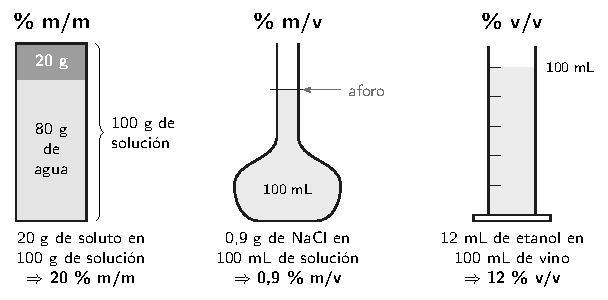
\includegraphics[max width=0.92\linewidth,max height=8.5cm]{qui/sol_porcentajes}
\end{center}
 
\begin{ojo}[{Siempre sobre la solución}] En las cuatro unidades el denominador es la \textbf{solución completa} (soluto + solvente), no el solvente solo.\end{ojo}
\subsection{Porcentaje masa/masa (\% m/m)}
Indica cuántos gramos de soluto hay en 100 g de solución:

 \[ \%\,\text{m/m} = \dfrac{m_{\text{soluto}}}{m_{\text{soluto}} + m_{\text{solvente}}}\cdot 100 \] 

\textbf{Ejemplo 1.} Se disuelven 25 g de sal en 100 g de agua. ¿Cuál es el \% m/m?

 

\textbf{Paso 1.} Masa de solución: $25 + 100 = 125$ g.

 

\textbf{Paso 2.} $\dfrac{25}{125}\cdot 100 = 20$ \%. La solución es 20 \% m/m.

 

\textbf{Ejemplo 2 (al revés).} ¿Cómo preparas 250 g de solución de azúcar al 8 \% m/m?

 

\textbf{Paso 1.} Soluto: $\dfrac{8}{100}\cdot 250 = 20$ g de azúcar.

 

\textbf{Paso 2.} Agua: lo que falta para 250 g, $250 - 20 = 230$ g.

 

\textbf{Comprobación:} $\dfrac{20}{20 + 230}\cdot 100 = \dfrac{20}{250}\cdot 100 = 8$ \%. \ding{52}

  
\begin{clave}[{Léelo como receta}] 20 \% m/m significa: 20 g de soluto por cada 100 g de solución, o sea, 20 g de soluto + 80 g de agua.\end{clave}
 
\begin{ojo}[{Error típico}] En el ejemplo 1, dividir por el agua da $\dfrac{25}{100}\cdot 100 = 25$ \%, que está mal: los 100 g son solo el solvente. La solución pesa 125 g.\end{ojo}
 
\begin{clave}[{}] La escala \textbf{Brix} de la industria del vino y los jugos es un \% m/m de azúcar: 1 °Bx es 1 g de azúcar en 100 g de solución.\end{clave}
\subsection{Porcentaje masa/volumen (\% m/v)}
Indica cuántos gramos de soluto hay en 100 mL de solución:

 \[ \%\,\text{m/v} = \dfrac{m_{\text{soluto}}\ (\text{g})}{V_{\text{solución}}\ (\text{mL})}\cdot 100 \] 

\textbf{Ejemplo 1.} El suero fisiológico es NaCl al 0,9 \% m/v. ¿Cuánto NaCl tiene una bolsa de 500 mL?

 

\textbf{Paso 1.} 0,9 g en cada 100 mL. 500 mL son 5 veces 100 mL.

 

\textbf{Paso 2.} $5 \cdot 0{,}9 = 4{,}5$ g de NaCl.

 

\textbf{Ejemplo 2.} Se disuelven 12 g de glucosa en agua hasta completar 300 mL de solución. ¿Cuál es el \% m/v?

 

\textbf{Paso 1.} $\dfrac{12}{300}\cdot 100 = 4$ \%. La solución es 4 \% m/v.

  
\begin{ojo}[{"Hasta completar" no es "se agregan"}] "Se disuelve en agua hasta completar 300 mL" significa que la \textbf{solución} mide 300 mL. "Se agregan 300 mL de agua" deja una solución de algo más de 300 mL. En \% m/v siempre va el volumen de la solución.\end{ojo}
 
\gatotip[\gatolila]{\textbf{Truco útil.} 4 \% m/v = 4 g en 100 mL = \textbf{40 g en 1 L}. Multiplicar el \% m/v por 10 te da los gramos por litro, y con eso pasas fácil a mol/L.}
\subsection{Porcentaje volumen/volumen (\% v/v)}
Se usa cuando el soluto es un líquido, como el alcohol en las bebidas. Indica cuántos mL de soluto hay en 100 mL de solución:

 \[ \%\,\text{v/v} = \dfrac{V_{\text{soluto}}\ (\text{mL})}{V_{\text{solución}}\ (\text{mL})}\cdot 100 \] 

\textbf{Ejemplo 1.} Un vino tiene 12 \% v/v de etanol (los "12 grados" de la etiqueta). ¿Cuánto etanol hay en una botella de 750 mL?

 

\textbf{Paso 1.} $\dfrac{12}{100}\cdot 750 = 90$ mL de etanol.

 

\textbf{Ejemplo 2.} Se mezclan 30 mL de etanol con agua hasta completar 200 mL. ¿Cuál es el \% v/v?

 

\textbf{Paso 1.} $\dfrac{30}{200}\cdot 100 = 15$ \%. La solución es 15 \% v/v.

  
\begin{ojo}[{Volúmenes que no se suman}] Al mezclar etanol y agua, el volumen final es un poco menor que la suma. Por eso las recetas dicen "completar hasta" un volumen. Si un problema dice "considere volúmenes aditivos", entonces sí puedes restar: en el vino, $750 - 90 = 660$ mL de agua.\end{ojo}
 
\begin{ejemplo}[{Ejemplo diario}] El alcohol gel al 70 \% v/v tiene 70 mL de etanol en cada 100 mL de gel.\end{ejemplo}
\subsection{Partes por millón (ppm)}
Para concentraciones muy bajas, como contaminantes o el flúor del agua potable, los porcentajes dan números incómodos. Se usan las \textbf{partes por millón}: 1 ppm es 1 g de soluto en 1.000.000 g de solución, o sea, \textbf{1 mg por kg}. En soluciones acuosas diluidas, 1 L pesa casi 1 kg, así que:

 \[ \text{ppm} = \dfrac{\text{mg de soluto}}{\text{L de solución}} \qquad \text{(o mg de soluto por kg, en sólidos)} \] 

\textbf{Ejemplo 1.} Un análisis encuentra 3 mg de ion fluoruro en 2 L de agua potable. $\dfrac{3\ \text{mg}}{2\ \text{L}} = 1{,}5$ ppm.

 

\textbf{Ejemplo 2.} La norma de agua potable permite hasta 0,01 mg/L de arsénico, es decir, 0,01 ppm. En 5 L de esa agua puede haber como máximo $0{,}01 \cdot 5 = 0{,}05$ mg.

  
\begin{clave}[{Para comparar}] 1 \% m/m = 1 g en 100 g = 10.000 mg en 1 kg = \textbf{10.000 ppm}.\end{clave}
 
\begin{ojo}[{Cuida las unidades}] ppm es mg por \textbf{litro} (no por mL) y por \textbf{miligramo} (no gramo). Si te dan mL, pásalos a L: 500 mL = 0,5 L. Si te dan gramos, pásalos a mg: 0,02 g = 20 mg.\end{ojo}
\subsection{La densidad: de volumen a masa}
Muchas veces te dan el volumen de una solución pero la concentración en \% m/m. La \textbf{densidad} conecta las dos cosas:

 \[ d = \dfrac{m}{V} \qquad\Rightarrow\qquad m = d\cdot V \] 

\textbf{Ejemplo.} Un frasco tiene 200 mL de solución de NaOH al 10 \% m/m, con densidad 1,2 g/mL. ¿Cuánto NaOH contiene y cuál es su \% m/v?

 

\textbf{Paso 1. Masa de la solución.} $m = 1{,}2 \cdot 200 = 240$ g.

 

\textbf{Paso 2. Masa de soluto.} El 10 \% de 240 g: $0{,}10 \cdot 240 = 24$ g de NaOH.

 

\textbf{Paso 3. \% m/v.} $\dfrac{24}{200}\cdot 100 = 12$ \% m/v.

 

\textbf{Comprobación:} \% m/v = \% m/m · densidad: $10 \cdot 1{,}2 = 12$. \ding{52}

  
\begin{ojo}[{¿Densidad de qué?}] Usa la densidad de la \textbf{solución}, no la del agua. El ácido clorhídrico comercial al 37 \% m/m tiene densidad cercana a 1,19 g/mL: 100 mL de él pesan unos 119 g, no 100 g.\end{ojo}
 
\begin{clave}[{Si d = 1 g/mL}] Los gramos y los mililitros de solución son el mismo número: 500 mL de solución pesan 500 g. Muchos problemas PAES lo dan así para simplificar.\end{clave}
\subsection{Lo clave del tema}
\begin{center}\small
\begin{tabularx}{\linewidth}{@{}>{\raggedright\arraybackslash\hsize=0.49\hsize}X>{\raggedright\arraybackslash\hsize=1.28\hsize}X>{\raggedright\arraybackslash\hsize=1.24\hsize}X@{}}
\toprule
\textbf{Unidad} & \textbf{Cálculo} & \textbf{Ejemplo} \\
\midrule
\% m/m & g soluto / g solución · 100 & 25 g en 100 g de agua \ensuremath{\rightarrow} 20 \% \\
\% m/v & g soluto / mL solución · 100 & 4,5 g en 500 mL \ensuremath{\rightarrow} 0,9 \% \\
\% v/v & mL soluto / mL solución · 100 & 90 mL en 750 mL \ensuremath{\rightarrow} 12 \% \\
ppm & mg soluto / L solución & 3 mg en 2 L \ensuremath{\rightarrow} 1,5 ppm \\
Densidad & m = d · V & 200 mL · 1,2 g/mL = 240 g \\
\bottomrule
\end{tabularx}
\end{center}
  
\begin{clave}[{Recuerda}] · \% m/m: divide por la masa de solución (soluto + agua).\par · 15 \% m/m son 15 g por cada 100 g de solución; escala a la masa real.\par · ppm = mg por L.\par · Si d \ensuremath{\neq} 1, pasa de mL a gramos con m = d · V.\end{clave}
 
\begin{clave}[{Método para la PAES}] 1. Anota qué es soluto y qué es solución, con unidades. 2. Elige la fórmula según la unidad pedida. 3. Pasa las unidades (mL \ensuremath{\leftrightarrow} L, g \ensuremath{\leftrightarrow} mg, volumen \ensuremath{\leftrightarrow} masa con la densidad). 4. Comprueba al revés: con tu resultado, ¿vuelves al dato?\end{clave}
\begin{elejemplo}{PAES Invierno 2027, adaptada}
Para preparar 0,5 L de una solución acuosa al 15 \% m/m de un compuesto soluble en agua (densidad de la solución = 1,0 g/mL), se deben mezclar
\alts{15 g del compuesto y 485 g de agua.}{75 g del compuesto y 500 g de agua.}{75 g del compuesto y 425 g de agua.}{15 g del compuesto y 85 g de agua.}
\solucion{\textbf{Paso 1. ¿Qué nos piden?} Las masas de compuesto (soluto) y de agua (solvente) que forman 0,5 L de solución al 15 \% m/m.

 

\textbf{Paso 2. Pasa el volumen a masa.} 0,5 L = 500 mL. Con la densidad: $m = d\cdot V = 1{,}0 \cdot 500 = 500$ g de solución.

 

\textbf{Paso 3. Masa de soluto.} 15 \% m/m es 15 g por cada 100 g de solución: $\dfrac{15}{100}\cdot 500 = 75$ g de compuesto.

 

\textbf{Paso 4. Masa de agua.} Lo que falta para completar 500 g: $500 - 75 = 425$ g de agua.

 

\textbf{Respuesta:} 75 g del compuesto y 425 g de agua.

 

\textbf{Comprobación:} $\dfrac{75}{75 + 425}\cdot 100 = \dfrac{75}{500}\cdot 100 = 15$ \%. \ding{52} Y la masa total, 500 g, con d = 1,0 g/mL ocupa 500 mL = 0,5 L. \ding{52}

 

\textbf{¿Por qué no las otras?} «15 g y 485 g» toma el 15 \% como 15 g totales: da $\dfrac{15}{500}\cdot 100 = 3$ \%. «75 g y 500 g» suma el soluto a 500 g de agua: la solución pesa 575 g y queda en $\dfrac{75}{575}\cdot 100 \approx 13$ \%. «15 g y 85 g» sí está al 15 \%, pero son solo 100 g de solución, no los 500 g pedidos.

\textbf{\color{cienciaD}Para recordar.} En \% m/m, masa de soluto = \% · masa de solución / 100, y el agua es lo que falta para completar la solución.}{C}
\end{elejemplo}

%% =====================================================================
%% qui_conc_quimicas
\section[Concentración molar, molal y fracción molar]{Concentración molar, molal y fracción molar}
\modcomun\ \ {\color{gris}\itshape Cómo pasar de gramos a moles y calcular la concentración molar (mol/L), la concentración molal (mol/kg de solvente) y la fracción molar; cómo se prepara una solución y cómo pasar de \% m/v a mol/L.\par}
\subsection{Del gramo al mol}
Las unidades químicas cuentan el soluto en \textbf{moles}, porque las reacciones ocurren partícula a partícula. Para pasar de gramos a moles se usa la \textbf{masa molar} ($M$, en g/mol):

 \[ n = \dfrac{m}{M} \] 

\textbf{Ejemplo 1.} Masa molar del NaOH (Na = 23, O = 16, H = 1): $23 + 16 + 1 = 40$ g/mol. Entonces 20 g de NaOH son $n = \dfrac{20}{40} = 0{,}5$ mol.

 

\textbf{Ejemplo 2.} Glucosa, C\textsubscript{6}H\textsubscript{12}O\textsubscript{6} (C = 12, H = 1, O = 16): $6\cdot 12 + 12\cdot 1 + 6\cdot 16 = 72 + 12 + 96 = 180$ g/mol. Entonces 9 g son $\dfrac{9}{180} = 0{,}05$ mol.

 

\textbf{Al revés:} $m = n \cdot M$. Por ejemplo, 0,1 mol de NaOH pesan $0{,}1 \cdot 40 = 4$ g.

  
\begin{ojo}[{Divide, no multipliques}] De gramos a moles se divide por la masa molar. Si multiplicas, $20 \cdot 40 = 800$, el número no tiene sentido: 20 g de algo no pueden ser 800 mol.\end{ojo}
 
\begin{clave}[{Masas molares que conviene tener a mano}] (la PAES las entrega)\par H\textsubscript{2}O = 18 g/mol · NaOH = 40 g/mol · NaCl = 58,5 g/mol · KOH = 56 g/mol · HCl = 36,5 g/mol · C\textsubscript{6}H\textsubscript{12}O\textsubscript{6} = 180 g/mol · C\textsubscript{2}H\textsubscript{5}OH = 46 g/mol\end{clave}
\subsection{Concentración molar (mol/L)}
La \textbf{concentración molar} (antes llamada molaridad) indica cuántos moles de soluto hay en \textbf{1 litro de solución}:

 \[ C = \dfrac{n_{\text{soluto}}\ (\text{mol})}{V_{\text{solución}}\ (\text{L})} \] 

\textbf{Ejemplo 1.} Se disuelven 20 g de NaOH ($M$ = 40 g/mol) en agua hasta completar 500 mL. Moles: $\dfrac{20}{40} = 0{,}5$ mol. Volumen: 500 mL = 0,5 L. $C = \dfrac{0{,}5}{0{,}5} = 1$ mol/L.

 

\textbf{Ejemplo 2 (al revés).} ¿Cuántos gramos de glucosa ($M$ = 180 g/mol) se necesitan para 250 mL de solución 0,2 mol/L? Moles: $n = C\cdot V = 0{,}2 \cdot 0{,}25 = 0{,}05$ mol. Masa: $0{,}05 \cdot 180 = 9$ g.

 
\begin{clave}[{Así se prepara}] 1. Masa el soluto. 2. Disuélvelo en un poco de agua dentro de un \textbf{matraz aforado}. 3. Agrega agua hasta la marca (el aforo). 4. Tapa y agita. Así el volumen final de solución es exacto.\end{clave}
  
\begin{center}
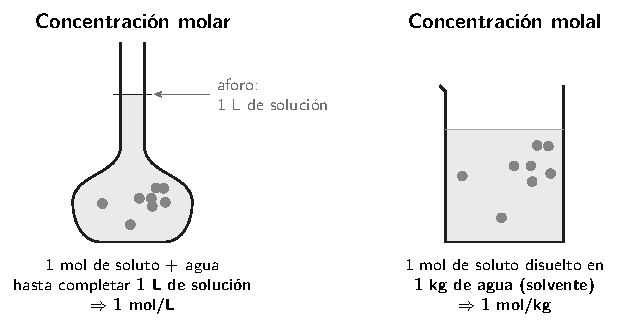
\includegraphics[max width=0.92\linewidth,max height=8.5cm]{qui/sol_molar_molal}
\end{center}
 
\begin{ojo}[{Dos errores clásicos}] 1. Dejar el volumen en mL: $\dfrac{0{,}5}{500} = 0{,}001$ está mal; pasa 500 mL a 0,5 L. 2. Disolver el soluto en 250 mL de agua: la solución queda con más de 250 mL. Se completa \textbf{hasta} 250 mL.\end{ojo}
\subsection{Concentración molal (mol/kg)}
La \textbf{concentración molal} (molalidad) indica cuántos moles de soluto hay por cada \textbf{kilogramo de solvente} (no de solución):

 \[ b = \dfrac{n_{\text{soluto}}\ (\text{mol})}{m_{\text{solvente}}\ (\text{kg})} \] 

\textbf{Ejemplo 1.} Se disuelven 20 g de NaOH ($M$ = 40 g/mol) en 500 g de agua. Moles: 0,5 mol. Solvente: 500 g = 0,5 kg. $b = \dfrac{0{,}5}{0{,}5} = 1$ mol/kg.

 

\textbf{Ejemplo 2.} 9 g de glucosa ($M$ = 180 g/mol) en 250 g de agua: $\dfrac{0{,}05}{0{,}25} = 0{,}2$ mol/kg.

  
\begin{center}\small
\begin{tabularx}{\linewidth}{@{}>{\raggedright\arraybackslash\hsize=1.09\hsize}X>{\raggedright\arraybackslash\hsize=1.01\hsize}X>{\raggedright\arraybackslash\hsize=0.89\hsize}X@{}}
\toprule
 & \textbf{Molar} & \textbf{Molal} \\
\midrule
Unidad & mol/L & mol/kg \\
Denominador & L de \textbf{solución} & kg de \textbf{solvente} \\
Se mide con & matraz aforado & balanza \\
¿Cambia con la temperatura? & Sí (el volumen se dilata) & No (la masa no cambia) \\
\bottomrule
\end{tabularx}
\end{center}
 
\begin{ojo}[{Ojo}] En molal el denominador es \textbf{solo el solvente} y va en \textbf{kilogramos}: 500 g de agua son 0,5 kg. Si divides por gramos, el resultado sale 1.000 veces más chico.\end{ojo}
\subsection{Fracción molar}
La \textbf{fracción molar} ($X$) de un componente es la parte de los moles totales que le corresponde:

 \[ X_{\text{soluto}} = \dfrac{n_{\text{soluto}}}{n_{\text{soluto}} + n_{\text{solvente}}} \] 

No tiene unidades, está entre 0 y 1, y las fracciones de todos los componentes \textbf{suman 1}.

 

\textbf{Ejemplo.} Se mezclan 46 g de etanol ($M$ = 46 g/mol) con 72 g de agua ($M$ = 18 g/mol).

 

\textbf{Paso 1. Moles.} Etanol: $\dfrac{46}{46} = 1$ mol. Agua: $\dfrac{72}{18} = 4$ mol. Total: 5 mol.

 

\textbf{Paso 2. Fracciones.} $X_{\text{etanol}} = \dfrac{1}{5} = 0{,}2$ y $X_{\text{agua}} = \dfrac{4}{5} = 0{,}8$.

 

\textbf{Comprobación:} $0{,}2 + 0{,}8 = 1$. \ding{52}

  
\begin{ojo}[{Tres errores frecuentes}] · Dividir por los moles del solvente: $\dfrac{1}{4} = 0{,}25$. El denominador es el \textbf{total}.\par · Usar masas en vez de moles: $\dfrac{46}{118} \approx 0{,}39$ es una fracción de masa, no molar.\par · Entregar la fracción del otro componente (0,8 en vez de 0,2).\end{ojo}
 
\begin{clave}[{Para qué sirve}] Se usa en mezclas de líquidos y de gases (el aire tiene $X_{\text{N}_2} \approx 0{,}78$) y en las propiedades que dependen del número de partículas.\end{clave}
\subsection{Pasar de una unidad a otra}
\textbf{De \% m/v a mol/L.} Multiplica el \% m/v por 10 para tener gramos por litro y divide por la masa molar.

 

\textbf{Ejemplo.} NaOH al 4 \% m/v ($M$ = 40 g/mol): 4 g en 100 mL = 40 g en 1 L. $\dfrac{40}{40} = 1$ mol en 1 L, o sea, \textbf{1 mol/L}.

 

\textbf{De mol/L a \% m/v.} NaCl 2 mol/L ($M$ = 58,5 g/mol): en 1 L hay $2\cdot 58{,}5 = 117$ g, o sea, 11,7 g en 100 mL: \textbf{11,7 \% m/v}.

 

\textbf{De \% m/m a mol/L, con densidad.} NaOH al 10 \% m/m con d = 1,2 g/mL. Toma 1 L de solución.

 

\textbf{Paso 1.} Masa de 1 L: $1{,}2 \cdot 1.000 = 1.200$ g.

 

\textbf{Paso 2.} Soluto: el 10 \% de 1.200 g = 120 g de NaOH.

 

\textbf{Paso 3.} Moles: $\dfrac{120}{40} = 3$ mol en 1 L: \textbf{3 mol/L}.

  
\begin{clave}[{Fórmula atajo}] $C\ (\text{mol/L}) = \dfrac{\%\,\text{m/v} \cdot 10}{M}$\end{clave}
 
\begin{ojo}[{Elige 1 L de base}] Cuando la concentración no depende de cuánto tengas, imagina 1 L (o 100 g) de solución: los cálculos salen con números redondos.\end{ojo}
\subsection{Lo clave del tema}
\begin{center}\small
\begin{tabularx}{\linewidth}{@{}>{\raggedright\arraybackslash\hsize=0.53\hsize}X>{\raggedright\arraybackslash\hsize=1.14\hsize}X>{\raggedright\arraybackslash\hsize=1.33\hsize}X@{}}
\toprule
\textbf{Unidad} & \textbf{Fórmula} & \textbf{Ejemplo} \\
\midrule
Moles & $n = m / M$ & 20 g de NaOH = 0,5 mol \\
Molar & mol de soluto / L de solución & 0,5 mol en 500 mL \ensuremath{\rightarrow} 1 mol/L \\
Molal & mol de soluto / kg de solvente & 0,5 mol en 500 g de agua \ensuremath{\rightarrow} 1 mol/kg \\
Fracción molar & $n_i$ / $n_{\text{total}}$, sin unidades & 1 mol etanol + 4 mol agua \ensuremath{\rightarrow} 0,2 \\
\% m/v \ensuremath{\rightarrow} mol/L & \% m/v · 10 / M & 4 \% de NaOH \ensuremath{\rightarrow} 1 mol/L \\
\bottomrule
\end{tabularx}
\end{center}
  
\begin{clave}[{Recuerda}] · Molaridad: primero pasa los gramos a moles ($m/M$).\par · Volumen en litros (molar) y masa de solvente en kg (molal).\par · Molalidad: divide solo por la masa del solvente.\par · Para preparar V mL de solución, completa hasta V mL en un matraz aforado.\end{clave}
 
\begin{clave}[{Método para la PAES}] 1. Pasa la masa a moles. 2. Mira el denominador que pide la unidad (L de solución, kg de solvente o moles totales). 3. Convierte unidades. 4. Comprueba al revés: $n = C\cdot V$ debe devolverte los moles.\end{clave}
\begin{elejemplo}{PAES Invierno 2027, adaptada}
En una clase de química, la profesora pide preparar 250 mL de una solución acuosa de hidróxido de sodio (NaOH) de concentración 0,4 mol/L (masa molar del NaOH = 40 g/mol). ¿Cuál de los siguientes procedimientos es el adecuado?
\altslargas{Masar 4 g de NaOH y disolverlos en 250 mL de agua.}{Masar 4 g de NaOH, disolverlos en un poco de agua dentro de un matraz aforado de 250 mL y luego agregar agua hasta el aforo.}{Masar 16 g de NaOH, disolverlos en un poco de agua dentro de un matraz aforado de 250 mL y luego agregar agua hasta el aforo.}{Masar 4 g de NaOH, disolverlos en agua y completar con agua hasta 1 L de solución.}
\solucion{\textbf{Paso 1. ¿Qué nos piden?} Dos cosas: la masa correcta de NaOH y la forma correcta de lograr 250 mL \textbf{de solución}.

 

\textbf{Paso 2. Moles necesarios.} $n = C\cdot V = 0{,}4\ \text{mol/L} \cdot 0{,}25\ \text{L} = 0{,}1$ mol.

 

\textbf{Paso 3. Masa.} $m = n\cdot M = 0{,}1 \cdot 40 = 4$ g de NaOH.

 

\textbf{Paso 4. Procedimiento.} El volumen de la fórmula es el de la \textbf{solución}. Por eso se disuelven los 4 g en un poco de agua dentro de un matraz aforado de 250 mL y se completa con agua hasta la marca: el volumen final es exactamente 250 mL.

 

\textbf{Respuesta:} masar 4 g de NaOH, disolverlos en un poco de agua dentro de un matraz aforado de 250 mL y agregar agua hasta el aforo.

 

\textbf{Comprobación:} $C = \dfrac{4/40}{0{,}25} = \dfrac{0{,}1}{0{,}25} = 0{,}4$ mol/L. \ding{52}

 

\textbf{¿Por qué no las otras?} «4 g en 250 mL de agua»: la masa está bien, pero el soluto agrega volumen y la solución queda con más de 250 mL, así que la concentración queda bajo 0,4 mol/L. «16 g hasta el aforo»: 16 g son 0,4 mol; en 0,25 L dan $\dfrac{0{,}4}{0{,}25} = 1{,}6$ mol/L (confunde 0,4 mol/L con 0,4 mol). «4 g hasta 1 L»: da $\dfrac{0{,}1}{1} = 0{,}1$ mol/L.

\textbf{\color{cienciaD}Para recordar.} Para preparar una solución: n = C · V, m = n · M, y se completa HASTA el volumen pedido en un matraz aforado.}{B}
\end{elejemplo}

%% =====================================================================
%% qui_dilucion
\section[Dilución y mezclas de soluciones]{Dilución y mezclas de soluciones}
\modcomun\ \ {\color{gris}\itshape Qué pasa al agregar agua a una solución, cómo usar C\textsubscript{1}·V\textsubscript{1} = C\textsubscript{2}·V\textsubscript{2} para calcular volúmenes y concentraciones, cuánta agua agregar, diluciones sucesivas y la concentración al mezclar soluciones del mismo soluto.\par}
\subsection{¿Qué es diluir?}
\textbf{Diluir} es agregar solvente a una solución. Pasan tres cosas:

 
\begin{itemize}
  \item Los \textbf{moles (y gramos) de soluto no cambian}: no agregaste soluto ni lo sacaste.
  \item El \textbf{volumen aumenta}.
  \item La \textbf{concentración baja}: el mismo soluto queda repartido en más volumen.
\end{itemize}
 

El \textbf{factor de dilución} dice cuántas veces creció el volumen: $\dfrac{V_2}{V_1}$. La concentración baja esas mismas veces. Si llevas 5 mL de una solución a 25 mL en un matraz aforado, el volumen crece 5 veces y la concentración queda en \textbf{un quinto} de la original, sea cual sea la unidad (\% m/m, mol/L\dots{}).

 

Lo contrario, \textbf{evaporar solvente}, sube la concentración: los moles siguen iguales en menos volumen.

  
\begin{center}
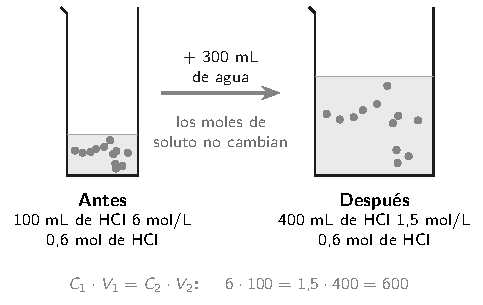
\includegraphics[max width=0.92\linewidth,max height=8.5cm]{qui/sol_dilucion}
\end{center}
 
\begin{ojo}[{Diluir no saca soluto}] "Al diluir hay menos soluto" es falso. Hay el mismo soluto; lo que hay es menos soluto \textbf{por cada mL}.\end{ojo}
\subsection{La fórmula C\textsubscript{1}·V\textsubscript{1} = C\textsubscript{2}·V\textsubscript{2}}
Como los moles no cambian, $n_1 = n_2$. Y como $n = C\cdot V$:

 \[ C_1 \cdot V_1 = C_2 \cdot V_2 \] 

El subíndice 1 es la solución inicial (concentrada) y el 2, la final (diluida). Con tres datos, despejas el cuarto.

 

\textbf{Ejemplo.} Tienes 100 mL de HCl 6 mol/L y quieres llevarlo a 1,5 mol/L. ¿Qué volumen final tendrá y cuánta agua agregas?

 

\textbf{Paso 1.} $6 \cdot 100 = 1{,}5 \cdot V_2$.

 

\textbf{Paso 2.} $V_2 = \dfrac{600}{1{,}5} = 400$ mL.

 

\textbf{Paso 3. Agua:} $V_2 - V_1 = 400 - 100 = 300$ mL.

 

\textbf{Comprobación:} moles antes, $6 \cdot 0{,}1 = 0{,}6$ mol; después, $1{,}5 \cdot 0{,}4 = 0{,}6$ mol. \ding{52}

  
\begin{clave}[{Unidades}] Los dos volúmenes deben ir en la misma unidad (los dos en mL o los dos en L), y las dos concentraciones también. No hace falta pasar a litros si ambos están en mL.\end{clave}
 
\begin{ojo}[{V\textsubscript{2} es el volumen final, no el agua}] El error más común es responder 400 mL cuando preguntan cuánta agua agregar. Agua = $V_2 - V_1$ (con volúmenes aditivos).\end{ojo}
\subsection{Cuánta agua agregar}
\textbf{Ejemplo 1.} Se tienen 0,5 L de H\textsubscript{2}SO\textsubscript{4} 4,0 mol/L y se necesita 0,2 mol/L. ¿Cuánta agua se agrega (volúmenes aditivos)?

 

\textbf{Paso 1.} $V_2 = \dfrac{C_1 V_1}{C_2} = \dfrac{4{,}0 \cdot 0{,}5}{0{,}2} = 10$ L.

 

\textbf{Paso 2.} Agua: $10 - 0{,}5 = 9{,}5$ L.

 

\textbf{Ejemplo 2, con \% m/v.} Se tienen 50 mL de NaOH al 4 \% m/v ($M$ = 40 g/mol) y se quiere 0,5 mol/L.

 

\textbf{Paso 1. Pasa a mol/L.} 4 \% m/v = 40 g/L = 1 mol/L.

 

\textbf{Paso 2.} $V_2 = \dfrac{1 \cdot 50}{0{,}5} = 100$ mL. Agua: $100 - 50 = 50$ mL.

  
\begin{clave}[{Preparar desde una solución madre}] Quieres 1 L de NaOH 0,03 mol/L a partir de NaOH 1,0 mol/L. $V_1 = \dfrac{0{,}03 \cdot 1.000}{1{,}0} = 30$ mL de solución madre, más agua hasta 1.000 mL: \textbf{30 mL + 970 mL de agua}. Mezclar 30 mL con 1.000 mL de agua daría 1.030 mL y una concentración un poco menor.\end{clave}
 
\begin{ojo}[{Las dos concentraciones en la misma unidad}] Si una está en \% m/v y la otra en mol/L, convierte primero.\end{ojo}
\subsection{Diluciones sucesivas y material}
A veces se diluye en dos pasos. Se resuelve un paso a la vez: la concentración final del primero es la inicial del segundo.

 

\textbf{Ejemplo.} A 500 mL de NaCl 1,5 mol/L se le agrega 1 L de agua (solución X). Luego se toman 10 mL de X y se completan con agua hasta 50 mL (solución Y). ¿Concentración de Y?

 

\textbf{Paso 1. Solución X.} Volumen: $500 + 1.000 = 1.500$ mL. $C_X = \dfrac{1{,}5 \cdot 500}{1.500} = 0{,}5$ mol/L.

 

\textbf{Paso 2. Solución Y.} $C_Y = \dfrac{0{,}5 \cdot 10}{50} = 0{,}1$ mol/L.

 

\textbf{Comprobación con factores:} el primer paso diluye 3 veces y el segundo 5 veces: en total 15 veces. $\dfrac{1{,}5}{15} = 0{,}1$. \ding{52}

  
\begin{clave}[{Material de laboratorio}] · \textbf{Pipeta} (aforada o graduada): para tomar un volumen exacto de la solución concentrada.\par · \textbf{Matraz aforado}: para completar un volumen final exacto. Es el material indispensable cuando la variable que se controla es el volumen final.\par · Vaso de precipitados y probeta: medidas aproximadas; no sirven para un volumen final exacto.\end{clave}
 
\begin{ojo}[{"Toma 10 mL de X"}] Tomar una parte de una solución no cambia su concentración: los 10 mL de X siguen siendo 0,5 mol/L.\end{ojo}
\subsection{Mezclas de soluciones del mismo soluto}
Al mezclar dos soluciones del \textbf{mismo soluto}, los moles se suman y los volúmenes también (si son aditivos):

 \[ C_f = \dfrac{C_1 V_1 + C_2 V_2}{V_1 + V_2} \] 
\begin{center}
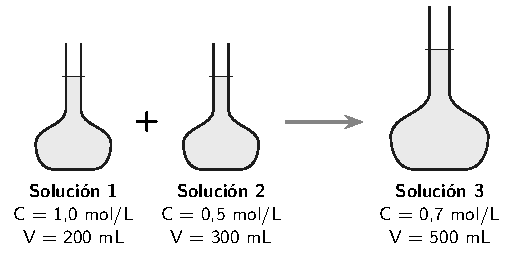
\includegraphics[max width=0.92\linewidth,max height=8.5cm]{qui/sol_mezcla_0}
\end{center}
 

\textbf{Ejemplo.} 200 mL de NaCl 1,0 mol/L + 300 mL de NaCl 0,5 mol/L.

 

\textbf{Paso 1. Moles.} $1{,}0 \cdot 0{,}2 = 0{,}2$ mol y $0{,}5 \cdot 0{,}3 = 0{,}15$ mol. Total: 0,35 mol.

 

\textbf{Paso 2. Volumen.} $0{,}2 + 0{,}3 = 0{,}5$ L.

 

\textbf{Paso 3.} $C_f = \dfrac{0{,}35}{0{,}5} = 0{,}7$ mol/L.

  
\begin{clave}[{Para comprobar}] La concentración final siempre queda \textbf{entre} las dos iniciales (0,5 < 0,7 < 1,0), más cerca de la que aporta más volumen. Si mezclas soluciones de \textbf{igual} concentración, la mezcla tiene esa misma concentración, aunque tenga el doble de soluto.\end{clave}
 
\begin{clave}[{Con tres soluciones}] 10 mL de HCl 1,0 mol/L + 20 mL de HCl 0,5 mol/L + 50 mL de HCl 0,2 mol/L: moles $0{,}01 + 0{,}01 + 0{,}01 = 0{,}03$ mol en 0,08 L: $\dfrac{0{,}03}{0{,}08} = 0{,}375$ mol/L.\end{clave}
 
\begin{ojo}[{No promedies las concentraciones}] $\dfrac{1{,}0 + 0{,}5}{2} = 0{,}75$ está mal, salvo que los volúmenes sean iguales. Suma moles y divide por el volumen total.\end{ojo}
\subsection{Lo clave del tema}
\begin{center}\small
\begin{tabularx}{\linewidth}{@{}>{\raggedright\arraybackslash\hsize=0.73\hsize}X>{\raggedright\arraybackslash\hsize=1.27\hsize}X@{}}
\toprule
\textbf{Situación} & \textbf{Qué hacer} \\
\midrule
Dilución & $C_1 V_1 = C_2 V_2$; los moles no cambian. \\
Agua a agregar & $V_2 - V_1$ (volúmenes aditivos). \\
Factor de dilución & $V_2 / V_1$: la concentración se divide por ese número. \\
Dos diluciones seguidas & Una a la vez, o multiplica los factores. \\
Mezcla del mismo soluto & $C_f = (C_1V_1 + C_2V_2)/(V_1 + V_2)$; queda entre las dos. \\
Evaporar solvente & Sube la concentración; los moles no cambian. \\
\bottomrule
\end{tabularx}
\end{center}
  
\begin{clave}[{Recuerda}] · El agua agregada es $V_2 - V_1$.\par · Al diluir, el volumen final es mayor que el inicial.\par · Al mezclar soluciones, suma moles y suma volúmenes.\par · Al diluir, los moles de soluto no cambian; solo baja la concentración.\end{clave}
 
\begin{clave}[{Método para la PAES}] 1. Escribe qué es 1 (inicial) y qué es 2 (final). 2. Iguala moles. 3. Fíjate si piden volumen final o agua agregada. 4. Comprueba: la concentración diluida debe ser menor y la de una mezcla, intermedia.\end{clave}
\begin{elejemplo}{PAES Invierno 2026, adaptada}
Algunos productos para el alisado del cabello contienen hidróxido de sodio (NaOH, masa molar = 40 g/mol), cuya concentración no debe superar cierto valor para evitar daños. Considerando volúmenes aditivos, ¿qué volumen de agua se debe agregar a 100 mL de una solución de NaOH al 2 \% m/v para obtener una solución de concentración 0,2 mol/L?
\alts{40 mL}{150 mL}{250 mL}{900 mL}
\solucion{\textbf{Paso 1. ¿Qué nos piden?} El volumen de \textbf{agua} que hay que agregar, no el volumen final. Las dos concentraciones vienen en unidades distintas, así que primero hay que igualarlas.

 

\textbf{Paso 2. Pasa el 2 \% m/v a mol/L.} 2 \% m/v son 2 g en 100 mL, o sea, 20 g en 1 L. En moles: $\dfrac{20}{40} = 0{,}5$ mol en 1 L. Entonces $C_1 = 0{,}5$ mol/L.

 

\textbf{Paso 3. Usa la dilución.} $C_1 V_1 = C_2 V_2$: $0{,}5 \cdot 100 = 0{,}2 \cdot V_2$, así que $V_2 = \dfrac{50}{0{,}2} = 250$ mL.

 

\textbf{Paso 4. Agua a agregar.} $250 - 100 = 150$ mL.

 

\textbf{Respuesta:} 150 mL.

 

\textbf{Comprobación:} moles de NaOH: al inicio, $0{,}5 \cdot 0{,}1 = 0{,}05$ mol (son los 2 g: $2/40 = 0{,}05$); al final, $0{,}2 \cdot 0{,}25 = 0{,}05$ mol. \ding{52}

 

\textbf{¿Por qué no las otras?} 250 mL es el volumen final, no el agua agregada. 40 mL despeja la fórmula al revés: $\dfrac{0{,}2 \cdot 100}{0{,}5}$, un volumen final menor que el inicial, lo que es imposible al diluir. 900 mL toma el 2 \% como si fuera 2 mol/L: $V_2 = \dfrac{2 \cdot 100}{0{,}2} = 1.000$ mL y resta 100 mL.

\textbf{\color{cienciaD}Para recordar.} Antes de usar C\textsubscript{1}V\textsubscript{1} = C\textsubscript{2}V\textsubscript{2}, pon las dos concentraciones en la misma unidad; y si piden agua, resta V\textsubscript{1}.}{B}
\end{elejemplo}

\chapter{Habilidades científicas}
%% =====================================================================
%% qui_hab_investigacion
\section[Investigar: preguntas, hipótesis y variables]{Investigar: preguntas, hipótesis y variables}
\modcomun\ \ {\color{gris}\itshape Cómo se arma una investigación en química: pregunta investigable, hipótesis y predicción, variables independiente, dependiente y controladas, grupo control, procedimiento e instrumentos, y la diferencia entre ley, teoría y modelo.\par}
\subsection{La investigación científica paso a paso}
Entre un cuarto y un tercio de las preguntas de la PAES de Ciencias no miden cuánta química sabes, sino si sabes \textbf{pensar como investigador}: reconocer la pregunta, la hipótesis, las variables y la conclusión de un experimento. Todas siguen el mismo esquema:

 
\begin{center}
\includegraphics[max width=0.92\linewidth,max height=8.5cm]{qui/hab_ciclo}
\end{center}
  

\textbf{Un ejemplo completo.}

 

\textbf{1. Observación.} Una estudiante nota que una tableta efervescente burbujea más rápido en agua tibia que en agua fría.

 

\textbf{2. Pregunta.} ¿Cómo influye la temperatura del agua en el tiempo que tarda la tableta en disolverse?

 

\textbf{3. Hipótesis.} A mayor temperatura del agua, menor es el tiempo de disolución.

 

\textbf{4. Predicción.} Si la hipótesis es correcta, la tableta se disolverá antes en agua a 40 °C que en agua a 10 °C.

 

\textbf{5. Procedimiento.} Pone tabletas iguales en 200 mL de agua a 10, 25 y 40 °C y mide con cronómetro el tiempo hasta que dejan de burbujear.

 

\textbf{6. Resultados.} 64 s, 40 s y 22 s.

 

\textbf{7. Conclusión.} En el rango estudiado, a mayor temperatura del agua, menor fue el tiempo de disolución: los datos apoyan la hipótesis.

  
\begin{clave}[{Pregunta investigable}] Es una pregunta que se puede responder \textbf{midiendo} algo. Casi siempre relaciona dos variables: «¿cómo influye A en B?».\end{clave}
 
\begin{clave}[{¿Investigable o no?}] · «¿Influye la concentración de HCl en la rapidez con que reacciona el magnesio?»: sí, se mide.\par · «¿Es el cobre el metal más bonito?»: no, es una opinión.\par · «¿Qué pasará con la química dentro de mil años?»: no, no se puede medir hoy.\end{clave}
 
\begin{ojo}[{Ojo}] La pregunta de investigación tiene que calzar con los datos. Si en la tabla solo cambia el tipo de fruta y se mide la vitamina C, la pregunta es «¿cómo varía la vitamina C en distintas frutas?», no «¿qué factores determinan la vitamina C?».\end{ojo}
\subsection{Hipótesis y predicción}
La \textbf{hipótesis} es una explicación o respuesta tentativa a la pregunta. Tiene tres rasgos:

 
\begin{itemize}
  \item Se escribe \textbf{antes} del experimento.
  \item Relaciona la variable que se cambia con la que se mide: «la concentración influye en la rapidez», «a mayor temperatura, mayor solubilidad».
  \item Se puede poner a prueba, y podría resultar falsa.
\end{itemize}
 

La \textbf{predicción} es más concreta: dice qué resultado se espera en \textbf{este} experimento si la hipótesis es cierta. Suele tener la forma «si\dots{}, entonces\dots{}».

 
\begin{center}\small
\begin{tabularx}{\linewidth}{@{}>{\raggedright\arraybackslash\hsize=1.00\hsize}X>{\raggedright\arraybackslash\hsize=1.00\hsize}X@{}}
\toprule
\textbf{Hipótesis} & \textbf{Predicción} \\
\midrule
La concentración de HCl influye en la rapidez de su reacción con magnesio. & Con HCl 2,0 mol/L el globo se inflará más en 1 minuto que con HCl 0,5 mol/L. \\
A menor tamaño de las partículas, más rápida es la disolución. & El azúcar flor se disolverá antes que el azúcar en terrones. \\
\bottomrule
\end{tabularx}
\end{center}
  
\begin{ejemplo}[{Ejemplo resuelto: ¿qué hipótesis se puso a prueba?}] Unos estudiantes preparan 100 mL de cuatro soluciones de KMnO\textsubscript{4} de 1,0; 0,2; 0,01 y 0,002 mol/L. Todas a 25 °C, agitadas 60 s, en frascos iguales y con la misma luz. Después observan la tonalidad.\par \textbf{Paso 1.} ¿Qué cambia de un frasco a otro? Solo la concentración.\par \textbf{Paso 2.} ¿Qué se observa? La tonalidad del color.\par \textbf{Paso 3.} La hipótesis une las dos: «la concentración de una solución influye en la tonalidad de su color».\par Las alternativas que hablan de temperatura, tiempo de agitación o luz son malas: esas variables se mantuvieron iguales.\end{ejemplo}
 
\begin{ojo}[{Hipótesis no es conclusión}] La hipótesis va antes de experimentar; la conclusión, después, apoyada en los datos. Un experimento no «demuestra» una hipótesis para siempre: la apoya o la contradice.\end{ojo}
\subsection{Variables: independiente, dependiente y controladas}
\begin{center}
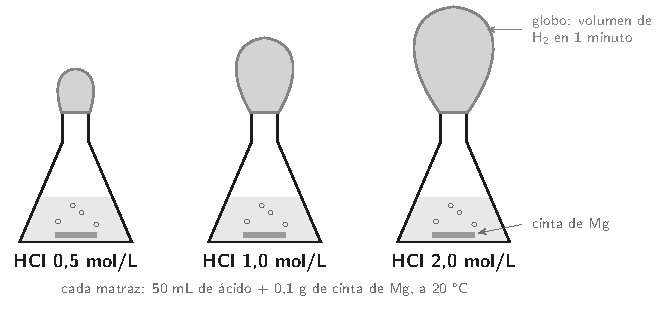
\includegraphics[max width=0.92\linewidth,max height=8.5cm]{qui/hab_globos}
\end{center}
  

En el montaje, un grupo pone 0,1 g de magnesio en 50 mL de HCl de tres concentraciones y mide cuánto se infla el globo con el H\textsubscript{2} formado en 1 minuto.

 
\begin{center}\small
\begin{tabularx}{\linewidth}{@{}>{\raggedright\arraybackslash\hsize=0.50\hsize}X>{\raggedright\arraybackslash\hsize=1.25\hsize}X>{\raggedright\arraybackslash\hsize=1.25\hsize}X@{}}
\toprule
\textbf{Variable} & \textbf{Cómo reconocerla} & \textbf{En el montaje} \\
\midrule
\textbf{Independiente} & La que el investigador \textbf{cambia a propósito} (la causa). & Concentración de HCl \\
\textbf{Dependiente} & La que se \textbf{mide} como respuesta (el efecto). & Volumen de H\textsubscript{2} (tamaño del globo) \\
\textbf{Controladas} & Las que se dejan \textbf{iguales} para que no influyan. & Masa de Mg, volumen de ácido, temperatura, tiempo \\
\bottomrule
\end{tabularx}
\end{center}
  
\gatotip[\gatoblanco]{\textbf{Truco de la frase.} Arma la frase «el efecto de \textbf{[independiente]} sobre \textbf{[dependiente]}». Aquí: «el efecto de la concentración de HCl sobre el volumen de H\textsubscript{2}». Si la frase no tiene sentido, cambiaste el orden.}
 
\begin{ejemplo}[{Ejemplo resuelto}] Se hacen reaccionar 1,5 g y 3 g del elemento Y con 2 g del elemento X, y se masa el compuesto formado.\par · Cambia a propósito: la masa de Y \ensuremath{\rightarrow} \textbf{independiente}.\par · Se mide al final: la masa de compuesto \ensuremath{\rightarrow} \textbf{dependiente}.\par · Siempre 2 g: la masa de X \ensuremath{\rightarrow} \textbf{controlada}.\end{ejemplo}
 
\begin{ojo}[{Ojo con las tablas}] La variable independiente suele ir en la primera columna y la dependiente en la última, pero no siempre. Pregúntate: ¿qué decidió el investigador \textbf{antes} de medir?\end{ojo}
\subsection{Grupo control, procedimiento e instrumentos}
El \textbf{grupo control} es el ensayo de comparación: igual a los demás, pero \textbf{sin} el factor que se estudia. Si quieres probar que el MnO\textsubscript{2} acelera la descomposición del H\textsubscript{2}O\textsubscript{2}, necesitas un tubo con H\textsubscript{2}O\textsubscript{2} y MnO\textsubscript{2} y otro tubo igual, con el mismo H\textsubscript{2}O\textsubscript{2} y a la misma temperatura, pero sin MnO\textsubscript{2}. Sin ese tubo no sabes si el MnO\textsubscript{2} hizo algo.

 

\textbf{Compara solo ensayos que se diferencian en una cosa.}

 
\begin{center}\small
\begin{tabular}{@{}lll@{}}
\toprule
\textbf{Ensayo} & \textbf{Temperatura} & \textbf{Azúcar} \\
\midrule
1 & 20 °C & granulada \\
2 & 40 °C & granulada \\
3 & 40 °C & flor (polvo) \\
\bottomrule
\end{tabular}
\end{center}
 

· 1 y 2: solo cambia la temperatura \ensuremath{\rightarrow} sirven para estudiar la temperatura.\par · 2 y 3: solo cambia el tamaño del grano \ensuremath{\rightarrow} sirven para el tamaño.\par · 1 y 3: cambian dos cosas \ensuremath{\rightarrow} no sirven: no sabrías cuál causó la diferencia.

  
\begin{clave}[{Instrumentos según la variable}] \begin{center}\small
\begin{tabularx}{\linewidth}{@{}>{\raggedright\arraybackslash\hsize=0.86\hsize}X>{\raggedright\arraybackslash\hsize=1.14\hsize}X@{}}
\toprule
\textbf{Para medir\dots{}} & \textbf{se usa\dots{}} \\
\midrule
masa & balanza \\
volumen de un líquido & probeta (aproximado), pipeta o bureta (preciso) \\
volumen exacto de una solución & matraz aforado \\
volumen de un gas & jeringa de gas, probeta invertida, cilindro con émbolo \\
temperatura & termómetro \\
tiempo & cronómetro \\
presión & barómetro o manómetro \\
acidez & pHmetro o papel indicador \\
\bottomrule
\end{tabularx}
\end{center}\end{clave}
 
\begin{ojo}[{Lee bien qué variable piden}] Si un gas se calienta a presión constante y se mide cómo cambia su volumen, el termómetro mide la variable independiente; la dependiente (el volumen) se mide con un cilindro graduado con émbolo móvil.\end{ojo}
\subsection{Ley, teoría, modelo y los demás componentes}
La PAES pregunta mucho «¿a qué componente de la investigación corresponde la frase entre comillas?». Apréndete esta tabla:

 
\begin{center}\small
\begin{tabularx}{\linewidth}{@{}>{\raggedright\arraybackslash\hsize=0.50\hsize}X>{\raggedright\arraybackslash\hsize=1.25\hsize}X>{\raggedright\arraybackslash\hsize=1.25\hsize}X@{}}
\toprule
\textbf{Componente} & \textbf{Qué es} & \textbf{Ejemplo en química} \\
\midrule
\textbf{Ley} & Describe una regularidad: \textbf{qué} pasa, a menudo con una fórmula. & Ley de conservación de la masa (Lavoisier); ley de las proporciones definidas (Proust); ley de Boyle. \\
\textbf{Teoría} & Explica \textbf{por qué} pasa; está respaldada por mucha evidencia. & Teoría atómica de Dalton; teoría cinético-molecular. \\
\textbf{Modelo} & Representación simplificada para explicar o predecir. & Modelo atómico de Bohr; modelo de esferas y varillas. \\
\textbf{Objetivo} & Lo que se quiere lograr; empieza con un verbo en infinitivo. & «Determinar la concentración de ácido acético de un vinagre». \\
\textbf{Procedimiento} & Los pasos que se siguen. & «Se quemó la muestra, se masaron el CO\textsubscript{2} y el H\textsubscript{2}O formados\dots{}». \\
\textbf{Observación} & Lo que se percibe o mide directamente. & «Se forma un sólido amarillo en el fondo del tubo». \\
\textbf{Resultado} & Los datos obtenidos. & «Las muestras del mar Rojo tienen entre 42 y 46 g/L de iones». \\
\textbf{Inferencia} & Interpretación que va más allá de lo observado. & «Casi todas las partículas alfa atraviesan la lámina: el átomo es mayormente vacío». \\
\textbf{Conclusión} & Respuesta a la pregunta, apoyada en los resultados. & «Estos cristales son yodo purificado mediante el procedimiento». \\
\bottomrule
\end{tabularx}
\end{center}
  
\begin{clave}[{Pistas en el texto}] · «si\dots{}, entonces\dots{} ocurrirá», «podría doblarse»: predicción.\par · «se agregó, se calentó, se midió»: procedimiento.\par · «se obtuvo», «los valores fueron»: resultado.\par · «por lo tanto», «esto indica», «corresponde a»: conclusión o inferencia.\end{clave}
  
\begin{ojo}[{Error típico}] Creer que una teoría es «una suposición» o que con más pruebas «se convierte en ley». No: la ley dice qué pasa y la teoría explica por qué. Son cosas distintas y ninguna pasa a ser la otra.\end{ojo}
\subsection{Lo clave del tema}
\begin{center}\small
\begin{tabularx}{\linewidth}{@{}>{\raggedright\arraybackslash\hsize=0.77\hsize}X>{\raggedright\arraybackslash\hsize=1.23\hsize}X@{}}
\toprule
\textbf{Concepto} & \textbf{Lo que tienes que reconocer} \\
\midrule
Pregunta de investigación & Se responde midiendo; calza con lo que se varió y lo que se midió. \\
Hipótesis & Respuesta tentativa que relaciona la variable independiente con la dependiente. \\
Predicción & Resultado concreto esperado: «si\dots{}, entonces\dots{}». \\
Variable independiente & La que se cambia a propósito. \\
Variable dependiente & La que se mide. \\
Variables controladas & Las que se mantienen iguales. \\
Grupo control & Ensayo sin el factor estudiado, para comparar. \\
Ley / teoría / modelo & Qué pasa / por qué pasa / representación simplificada. \\
\bottomrule
\end{tabularx}
\end{center}
 
\begin{clave}[{Recuerda}] · Variable independiente: la que se decide antes; dependiente: la que se mide.\par · La hipótesis habla de la variable que cambia en el experimento.\par · Para estudiar una variable, compara ensayos que solo difieren en esa variable.\par · «El pH fue 5,2» es un resultado; la conclusión lo interpreta y responde la pregunta.\par · Cada variable se mide con su instrumento: la temperatura con termómetro, el volumen con probeta.\end{clave}
 
\begin{clave}[{Método PAES}] 1. Subraya qué se cambió, qué se midió y qué se dejó igual. 2. Con eso, nombra las tres variables. 3. Si preguntan por la hipótesis o la pregunta, elige la que relaciona exactamente esas dos variables. 4. Si preguntan por un componente, busca las pistas («si\dots{} entonces», «se obtuvo», «se agregó»). 5. Descarta las alternativas que hablan de variables que no cambiaron.\end{clave}
\begin{elejemplo}{PAES Invierno 2027, adaptada}
En la producción de litio se precipita carbonato de litio, Li\textsubscript{2}CO\textsubscript{3}, desde una solución acuosa. Como este compuesto es bastante soluble en agua, un grupo de investigadores estudia qué parámetros permiten disminuir su solubilidad. En la tabla se presentan las condiciones de cuatro ensayos:
\begin{center}\small
\begin{tabularx}{\linewidth}{@{}>{\raggedright\arraybackslash\hsize=0.39\hsize}X>{\raggedright\arraybackslash\hsize=0.69\hsize}X>{\raggedright\arraybackslash\hsize=1.20\hsize}X>{\raggedright\arraybackslash\hsize=1.72\hsize}X@{}}
\toprule
\textbf{Ensayo} & \textbf{Temperatura (°C)} & \textbf{Velocidad de agitación (rpm)} & \textbf{Concentración inicial de Li\textsubscript{2}CO\textsubscript{3} (mol/L)} \\
\midrule
\textbf{1} & 25 & 150 & 2 \\
\textbf{2} & 25 & 300 & 2 \\
\textbf{3} & 45 & 150 & 2 \\
\textbf{4} & 45 & 300 & 1 \\
\bottomrule
\end{tabularx}
\end{center}
\altslargas{Comparar los ensayos 1 y 2 permite analizar el efecto de la temperatura.}{Comparar los ensayos 2 y 4 permite analizar el efecto de la concentración.}{Comparar los ensayos 1 y 3 permite analizar el efecto de la temperatura.}{Comparar los ensayos 3 y 4 permite analizar el efecto de la velocidad de agitación.}
\solucion{\textbf{Paso 1. ¿Qué nos piden?} Elegir un par de ensayos que sirva para estudiar el efecto de \textbf{un} parámetro. La regla de oro: dos ensayos sirven para estudiar una variable solo si se diferencian \textbf{únicamente} en esa variable. Así, si el resultado cambia, sabemos qué lo causó.

\textbf{Paso 2. Ensayos 1 y 2.} Temperatura: 25 y 25 (igual). Agitación: 150 y 300 (cambia). Concentración: 2 y 2 (igual). Solo cambia la agitación: este par sirve para la \textbf{agitación}, no para la temperatura.

\textbf{Paso 3. Ensayos 2 y 4.} Temperatura: 25 y 45 (cambia). Agitación: 300 y 300 (igual). Concentración: 2 y 1 (cambia). Cambian dos parámetros a la vez: este par no sirve para nada, porque no sabríamos cuál causó la diferencia.

\textbf{Paso 4. Ensayos 1 y 3.} Temperatura: 25 y 45 (cambia). Agitación: 150 y 150 (igual). Concentración: 2 y 2 (igual). Solo cambia la temperatura: este par sirve para estudiar la \textbf{temperatura}. \ding{52}

\textbf{Paso 5. Ensayos 3 y 4.} Temperatura: 45 y 45 (igual). Agitación: 150 y 300 (cambia). Concentración: 2 y 1 (cambia). Cambian dos parámetros: no sirve.

\textbf{Respuesta:} comparar los ensayos 1 y 3 permite analizar el efecto de la temperatura.

\textbf{Comprobación:} en los ensayos 1 y 3 la temperatura es la variable independiente y la agitación (150 rpm) y la concentración inicial (2 mol/L) son variables controladas. Es justo el diseño que se necesita.

\textbf{¿Por qué no las otras?} «1 y 2 para la temperatura» se equivoca de variable: en ese par la temperatura es igual (25 °C) y lo único que cambia es la agitación. «2 y 4 para la concentración» y «3 y 4 para la agitación» eligen pares en los que cambian dos parámetros a la vez; cualquier diferencia en la solubilidad podría deberse a cualquiera de los dos.

\textbf{\color{cienciaD}Para recordar.} Para estudiar una variable, compara solo ensayos que se diferencian únicamente en esa variable.}{C}
\end{elejemplo}

%% =====================================================================
%% qui_hab_evidencia
\section[Procesar y analizar la evidencia]{Procesar y analizar la evidencia}
\modcomun\ \ {\color{gris}\itshape Leer tablas y gráficos de experimentos químicos, reconocer tendencias y relaciones directas, inversas y proporcionales, hacer predicciones e inferencias y sacar conclusiones que se sostienen con los datos.\par}
\subsection{Leer una tabla de datos}
Antes de mirar las alternativas, lee la tabla en cuatro pasos:

 

\textbf{Paso 1. Encabezados y unidades.} ¿Qué mide cada columna? ¿En qué unidad?

 

\textbf{Paso 2. ¿Qué cambia y qué se mide?} Identifica la variable independiente y la dependiente.

 

\textbf{Paso 3. Recorre en orden.} Sigue la columna que crece y mira qué hace la otra: ¿sube, baja o queda igual?

 

\textbf{Paso 4. Revisa todas las filas.} Una tendencia vale solo si se cumple en todas.

 
\begin{center}\small
\begin{tabularx}{\linewidth}{@{}>{\raggedright\arraybackslash\hsize=0.56\hsize}X>{\raggedright\arraybackslash\hsize=1.40\hsize}X>{\raggedright\arraybackslash\hsize=1.21\hsize}X>{\raggedright\arraybackslash\hsize=0.84\hsize}X@{}}
\toprule
\textbf{Compuesto} & \textbf{Temperatura de ebullición (°C)} & \textbf{Temperatura de fusión (°C)} & \textbf{Propiedad X (u.a.)} \\
\midrule
NaF & 1705 & 990 & 2,21 \\
NaCl & 1413 & 801 & 2,81 \\
NaBr & 1390 & 755 & 2,97 \\
NaI & 1300 & 651 & 3,23 \\
\bottomrule
\end{tabularx}
\end{center}
  
\begin{ejemplo}[{Ejemplo resuelto}] En la tabla, la propiedad X crece de arriba hacia abajo: 2,21 \ensuremath{\rightarrow} 2,81 \ensuremath{\rightarrow} 2,97 \ensuremath{\rightarrow} 3,23. Mientras tanto, la temperatura de ebullición baja (1705 \ensuremath{\rightarrow} 1300) y la de fusión también (990 \ensuremath{\rightarrow} 651).\par Relaciones correctas:\par · «La temperatura de ebullición \textbf{disminuye} al aumentar la propiedad X».\par · «La temperatura de fusión \textbf{aumenta} al disminuir la propiedad X» (es lo mismo, leído al revés).\end{ejemplo}
 
\begin{ojo}[{La trampa del «al disminuir»}] «La temperatura de fusión disminuye al disminuir X» es \textbf{falsa}: si X baja, la temperatura sube. Cuando una alternativa recorre la tabla al revés, recórrela tú también al revés antes de responder.\end{ojo}
\subsection{Leer un gráfico}
\begin{center}
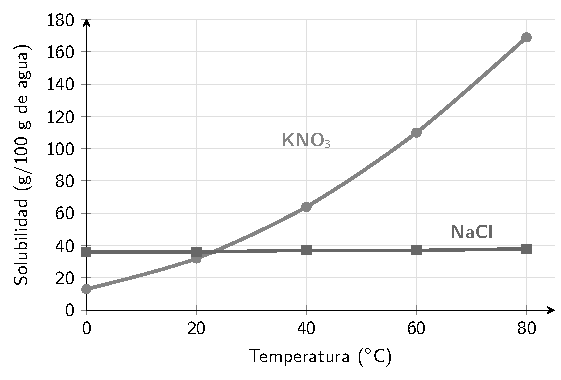
\includegraphics[max width=0.92\linewidth,max height=8.5cm]{qui/hab_solubilidad}
\end{center}
 

\textbf{Paso 1. Ejes.} Eje horizontal: temperatura (°C), la variable independiente. Eje vertical: solubilidad, en gramos de sal por 100 g de agua, la variable dependiente.

 

\textbf{Paso 2. Escala.} Cada línea horizontal vale 20 g; cada vertical, 20 °C.

 

\textbf{Paso 3. Lee puntos.} A 60 °C se disuelven como máximo 110 g de KNO\textsubscript{3} en 100 g de agua. A 20 °C, solo 32 g.

 

\textbf{Paso 4. Compara curvas.} Las curvas se cruzan cerca de 22 °C: por debajo de esa temperatura el NaCl es más soluble; por encima, el KNO\textsubscript{3}.

  
\begin{clave}[{La pendiente cuenta la historia}] La curva del KNO\textsubscript{3} sube mucho: su solubilidad depende fuertemente de la temperatura. La del NaCl es casi plana (36 a 38 g): casi no cambia.\end{clave}
 
\begin{ejemplo}[{Ejemplo resuelto}] Una solución saturada de KNO\textsubscript{3} en 100 g de agua a 60 °C se enfría hasta 40 °C. ¿Cuánto KNO\textsubscript{3} cristaliza?\par \textbf{Paso 1.} A 60 °C hay disueltos 110 g.\par \textbf{Paso 2.} A 40 °C caben solo 64 g.\par \textbf{Paso 3.} Cristaliza la diferencia: $110 - 64 = 46$ g.\end{ejemplo}
 
\begin{ojo}[{Ojo con la cantidad de agua}] El gráfico es «por 100 g de agua». Con 50 g de agua cabe la mitad: a 60 °C, 55 g de KNO\textsubscript{3}, no 110 g.\end{ojo}
\subsection{Relaciones entre variables}
\begin{center}
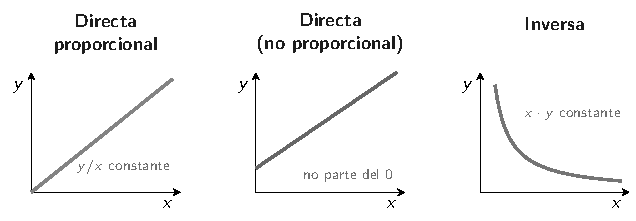
\includegraphics[max width=0.92\linewidth,max height=8.5cm]{qui/hab_relaciones}
\end{center}
  
\begin{center}\small
\begin{tabularx}{\linewidth}{@{}>{\raggedright\arraybackslash\hsize=0.71\hsize}X>{\raggedright\arraybackslash\hsize=1.14\hsize}X>{\raggedright\arraybackslash\hsize=1.14\hsize}X@{}}
\toprule
\textbf{Relación} & \textbf{Qué pasa} & \textbf{Cómo comprobarla} \\
\midrule
Directa & Si una aumenta, la otra también. & Ambas columnas suben juntas. \\
Directamente proporcional & Si una se duplica, la otra se duplica. & El cociente $y/x$ es constante; el gráfico es una recta que pasa por el origen. \\
Inversa & Si una aumenta, la otra disminuye. & Una columna sube y la otra baja. \\
Inversamente proporcional & Si una se duplica, la otra se reduce a la mitad. & El producto $x\cdot y$ es constante. \\
\bottomrule
\end{tabularx}
\end{center}
  
\begin{ejemplo}[{Ejemplo resuelto}] Un gas a temperatura constante:
\begin{center}\small
\begin{tabular}{@{}lll@{}}
\toprule
\textbf{Presión (atm)} & \textbf{Volumen (L)} & \textbf{$P\cdot V$} \\
\midrule
1 & 12 & 12 \\
2 & 6 & 12 \\
3 & 4 & 12 \\
\bottomrule
\end{tabular}
\end{center}
 El producto es siempre 12: el volumen es \textbf{inversamente proporcional} a la presión (ley de Boyle).\end{ejemplo}
 
\begin{ojo}[{No todo lo directo es proporcional}] La temperatura de ebullición de los alcanos sube con el número de carbonos, pero el propano hierve a \ensuremath{-}42 °C: el gráfico no pasa por el origen. Es una relación directa, no proporcional. Lo mismo con las inversas: que una baje cuando la otra sube no basta; el producto tiene que ser constante.\end{ojo}
\subsection{Tendencias: interpolar y predecir}
Una \textbf{tendencia} es el patrón que siguen los datos. Con ella se puede estimar un valor que no se midió.

 
\begin{itemize}
  \item \textbf{Interpolar}: estimar un valor \textbf{dentro} del rango medido. Es bastante seguro.
  \item \textbf{Extrapolar}: estimar \textbf{fuera} del rango medido. Es arriesgado, y solo vale para valores cercanos.
\end{itemize}
 
\begin{center}\small
\begin{tabular}{@{}lll@{}}
\toprule
\textbf{Alcano lineal} & \textbf{N.º de C} & \textbf{Temperatura de ebullición (°C)} \\
\midrule
Pentano & 5 & 36 \\
Hexano & 6 & 69 \\
Heptano & 7 & 98 \\
Octano & 8 & 126 \\
\bottomrule
\end{tabular}
\end{center}
 

Las diferencias son 33, 29 y 28 °C: cada carbono extra sube la temperatura de ebullición en unos 30 °C, y el salto se achica poco a poco. Para el nonano (9 C) se espera algo más de 150 °C. El valor real es 151 °C.

  
\begin{ejemplo}[{Ejemplo resuelto: predecir con dos tendencias}] \begin{center}\small
\begin{tabular}{@{}llll@{}}
\toprule
\textbf{Lineal} & \textbf{°C} & \textbf{Con una ramificación} & \textbf{°C} \\
\midrule
Pentano & 36,1 & 2-metilbutano & 27,8 \\
Hexano & 68,7 & 2-metilpentano & 60,3 \\
Heptano & 98,4 & 2-metilhexano & ? \\
\bottomrule
\end{tabular}
\end{center}
\textbf{Paso 1.} La ramificación baja la temperatura de ebullición en unos 8,4 °C: $36{,}1 - 27{,}8 = 8{,}3$ y $68{,}7 - 60{,}3 = 8{,}4$.\par \textbf{Paso 2.} Para el 2-metilhexano: $98{,}4 - 8{,}4 = 90{,}0$ °C. El valor real es 90,0 °C.\end{ejemplo}
 
\begin{ojo}[{No extrapoles lejos}] Que tres datos bajen no significa que sigan bajando hasta cero ni que sigan igual a 200 °C. La conclusión vale para el rango estudiado.\end{ojo}
\subsection{De los datos a la conclusión}
Una \textbf{conclusión} o \textbf{inferencia} correcta cumple tres condiciones:

 
\begin{itemize}
  \item \textbf{Sale de los datos.} Lo que afirma se puede ver en la tabla o el gráfico.
  \item \textbf{Habla solo de lo que se midió.} Las mismas variables y el mismo rango; si se midió a 1 y a 8 horas, vale «en los dos tiempos estudiados».
  \item \textbf{No agrega cosas.} Ni síntomas, ni «siempre», ni «todas las sustancias», ni causas que el experimento no puso a prueba.
\end{itemize}
 
\begin{ejemplo}[{Ejemplo resuelto: reactivo limitante}] BaCl\textsubscript{2} + Na\textsubscript{2}SO\textsubscript{4} \ensuremath{\rightarrow} BaSO\textsubscript{4} + 2 NaCl, todo en razón 1 : 1.
\begin{center}\small
\begin{tabular}{@{}llll@{}}
\toprule
\textbf{Tubo} & \textbf{BaCl\textsubscript{2} (mol)} & \textbf{Na\textsubscript{2}SO\textsubscript{4} (mol)} & \textbf{BaSO\textsubscript{4} (mol)} \\
\midrule
1 & 0,0001 & 0,0009 & 0,0001 \\
3 & 0,0003 & 0,0007 & 0,0003 \\
5 & 0,0005 & 0,0005 & 0,0005 \\
\bottomrule
\end{tabular}
\end{center}
 El precipitado coincide siempre con el BaCl\textsubscript{2}, que es el que está en menor cantidad: la cantidad de precipitado depende del \textbf{reactivo limitante}, el BaCl\textsubscript{2}.\end{ejemplo}
  
\begin{ejemplo}[{Ejemplo resuelto: proporción constante}] Dos ensayos combinan 0,25 mol de Y con 0,50 mol de X, y 0,50 mol de Y con 1,00 mol de X. En ambos, $\dfrac{n_X}{n_Y} = 2$: X e Y se combinan en la misma proporción (2 : 1) en los dos ensayos. Es la ley de las proporciones definidas.\end{ejemplo}
 
\begin{ojo}[{Palabras sospechosas}] «Siempre», «todos», «demuestra definitivamente», «cualquier tipo de\dots{}», «se vuelve irreversible». Si la tabla no lo muestra, la alternativa es falsa aunque suene científica.\end{ojo}
 
\begin{ojo}[{Correlación no es causa}] Que dos variables cambien juntas no prueba que una cause la otra, salvo que el experimento haya cambiado una y controlado todo lo demás.\end{ojo}
\subsection{Cálculos rápidos con los datos}
Muchas preguntas de evidencia piden comparar \textbf{cocientes}, no los números de la tabla. Sin calculadora, simplifica las fracciones.

 
\begin{ejemplo}[{Ejemplo resuelto: eficiencia}] Cuatro métodos producen hidrógeno a partir de agua. ¿Cuál es más eficiente?
\begin{center}\small
\begin{tabular}{@{}llll@{}}
\toprule
\textbf{Método} & \textbf{Agua usada (L)} & \textbf{H\textsubscript{2} producido (mol)} & \textbf{mol por litro} \\
\midrule
1 & 10 & 0,8 & 0,08 \\
2 & 12 & 1,0 & 0,083 \\
3 & 15 & 1,5 & 0,10 \\
4 & 25 & 1,8 & 0,072 \\
\bottomrule
\end{tabular}
\end{center}
 El método 4 produce más hidrógeno en total, pero gasta mucha más agua. Por cada litro, el más eficiente es el \textbf{método 3}.\end{ejemplo}
  
\begin{ejemplo}[{Ejemplo resuelto: porcentaje en masa}] Al quemar 0,70 g de hierro se forma 1,00 g de óxido. Porcentaje de hierro: $\dfrac{0{,}70}{1{,}00}\cdot 100 = 70\%$. Si otro ensayo da 7,78 g de hierro en 10,00 g de óxido, el porcentaje es 77,8 \%: se formó un óxido distinto.\end{ejemplo}
 
\gatotip[\gatonaranjo]{\textbf{Trucos sin calculadora.} · Para comparar $\dfrac{0{,}8}{10}$ con $\dfrac{1{,}0}{12}$, multiplica en cruz: $0{,}8\cdot 12 = 9{,}6$ y $1{,}0\cdot 10 = 10$. Como $9{,}6 < 10$, la primera fracción es menor.\par · Para un porcentaje, lleva el denominador a 100: $\dfrac{3{,}89}{5} = \dfrac{77{,}8}{100} = 77{,}8\%$.}
 
\begin{ojo}[{Error típico}] Elegir la fila con el número más grande. «Más eficiente», «mayor rendimiento» y «mayor porcentaje» piden un cociente, no un total.\end{ojo}
\subsection{Lo clave del tema}
\begin{center}\small
\begin{tabularx}{\linewidth}{@{}>{\raggedright\arraybackslash\hsize=0.95\hsize}X>{\raggedright\arraybackslash\hsize=1.05\hsize}X@{}}
\toprule
\textbf{Si te piden\dots{}} & \textbf{Haz esto} \\
\midrule
Una relación o tendencia & Recorre la variable que crece y mira qué hace la otra; revisa todas las filas. \\
Saber si es proporcional & Directa: cociente constante, recta por el origen. Inversa: producto constante. \\
Leer un gráfico & Ejes, unidades y escala antes de leer un punto. \\
Una predicción & Sigue la tendencia (diferencias entre valores seguidos), sin extrapolar lejos. \\
Una conclusión o inferencia & Que salga de los datos, hable solo de lo medido y no agregue nada. \\
Eficiencia, rendimiento o porcentaje & Calcula un cociente para cada fila y compara. \\
\bottomrule
\end{tabularx}
\end{center}
 
\begin{clave}[{Recuerda}] · En una relación inversa, cuando una variable disminuye, la otra aumenta.\par · Una relación es proporcional solo si el cociente entre las variables es constante.\par · Las curvas de solubilidad se leen por 100 g de agua: si caben 110 g de KNO\textsubscript{3} en 100 g, en 50 g caben 55 g.\par · La conclusión se limita a lo estudiado: «en el rango estudiado, la solubilidad del KNO\textsubscript{3} aumenta con la temperatura».\par · La eficiencia se compara con lo producido por unidad de lo gastado.\end{clave}
 
\begin{clave}[{Método PAES}] 1. Lee encabezados, ejes y unidades. 2. Identifica qué cambió y qué se midió. 3. Describe en tu cabeza la tendencia antes de leer las alternativas. 4. Si hay números, calcula el cociente, la diferencia o el producto que corresponda. 5. Descarta lo que no sale de los datos, lo que generaliza y lo que habla de variables que no se midieron.\end{clave}
\begin{elejemplo}{PAES Invierno 2027, adaptada}
Un estudiante encuentra en un libro la temperatura de ebullición, a 1 atm, de un conjunto de alcanos de cadena lineal, no ramificados, cuyos átomos de carbono están unidos entre sí solo por enlaces simples C--C. Con esa información elabora el siguiente gráfico:
\begin{center}
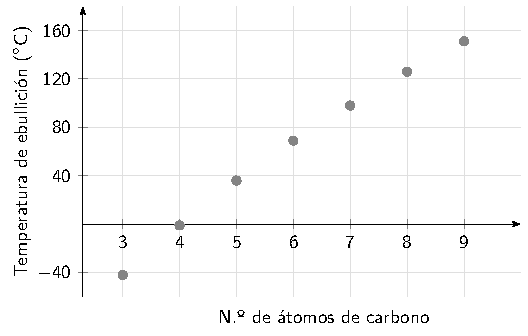
\includegraphics[max width=0.92\linewidth,max height=8.5cm]{qui/hab_alcanos}
\end{center}
\altslargas{A medida que aumenta el número de átomos de carbono, la temperatura de ebullición es menor que cero.}{A medida que disminuye el número de átomos de carbono, la temperatura de ebullición disminuye.}{La temperatura de ebullición es directamente proporcional al número de átomos de carbono.}{La temperatura de ebullición se mantiene constante para los alcanos con más de 7 átomos de carbono.}
\solucion{\textbf{Paso 1. ¿Qué nos piden?} La afirmación que describe correctamente la tendencia del gráfico. Primero leemos el gráfico y después revisamos cada alternativa.

\textbf{Paso 2. Lee los ejes.} Eje horizontal: número de átomos de carbono (3 a 9). Eje vertical: temperatura de ebullición en °C. Cada línea vale 40 °C.

\textbf{Paso 3. Lee los puntos.} 3 C: unos \ensuremath{-}42 °C. 4 C: casi 0 °C. 5 C: 36 °C. 6 C: 69 °C. 7 C: 98 °C. 8 C: 126 °C. 9 C: 151 °C.

\textbf{Paso 4. Describe la tendencia.} De izquierda a derecha, los puntos siempre suben: al aumentar el número de carbonos aumenta la temperatura de ebullición. Leído al revés, al disminuir el número de carbonos, la temperatura de ebullición disminuye. Es una relación directa.

\textbf{Paso 5. Revisa la relación con números.} ¿Es proporcional? Si lo fuera, el cociente temperatura/carbonos sería constante y la recta pasaría por el origen. Pero con 3 C el valor es negativo (\ensuremath{-}42 °C) y con 4 C es casi 0 °C: no es proporcional.

\textbf{Respuesta:} a medida que disminuye el número de átomos de carbono, la temperatura de ebullición disminuye.

\textbf{Comprobación:} recorre el gráfico de derecha a izquierda: 151 \ensuremath{\rightarrow} 126 \ensuremath{\rightarrow} 98 \ensuremath{\rightarrow} 69 \ensuremath{\rightarrow} 36 \ensuremath{\rightarrow} \ensuremath{-}1 \ensuremath{\rightarrow} \ensuremath{-}42. Siempre baja. \ding{52} La explicación química: con más carbonos la molécula es más grande, las fuerzas entre moléculas son mayores y cuesta más separarlas.

\textbf{¿Por qué no las otras?} «Es menor que cero» es falsa: solo el propano (y, apenas, el butano) quedan bajo cero; desde 5 C todos están sobre cero. «Directamente proporcional» confunde relación directa con proporcional: al duplicar los carbonos de 4 a 8, la temperatura no se duplica (pasa de unos 0 °C a 126 °C), y el gráfico no pasa por el origen. «Se mantiene constante sobre 7 C» es falsa: de 7 a 9 C sigue subiendo, de 98 a 151 °C.

\textbf{\color{cienciaD}Para recordar.} Describe la tendencia en las dos direcciones y no confundas una relación directa con una proporcional.}{B}
\end{elejemplo}

%% =====================================================================
%% qui_hab_evaluar
\section[Evaluar y comunicar una investigación]{Evaluar y comunicar una investigación}
\modcomun\ \ {\color{gris}\itshape Juzgar la validez y la confiabilidad de un experimento químico, decidir si una conclusión se sostiene con los datos, reconocer limitaciones del diseño y cómo mejorarlo, la reproducibilidad, los alcances tecnológicos y el recurso adecuado para comunicar resultados.\par}
\subsection{Validez y confiabilidad}
\textbf{Validez:} la investigación mide de verdad lo que dice medir y su diseño permite sacar la conclusión. Falla cuando no se controlaron variables, cuando falta un grupo control o cuando se mide otra cosa.

 

\textbf{Confiabilidad:} al repetir las mediciones se obtienen resultados parecidos. Depende de cuántas veces se repite, del tamaño de la muestra y de la precisión de los instrumentos.

 

\textbf{Precisión y exactitud.} Mediciones \textbf{precisas} son cercanas entre sí. Mediciones \textbf{exactas} son cercanas al valor real. Se puede ser preciso sin ser exacto, por ejemplo con una balanza mal calibrada que siempre marca 0,5 g de más.

 
\begin{center}\small
\begin{tabular}{@{}ll@{}}
\toprule
\textbf{Instrumento} & \textbf{Lectura típica} \\
\midrule
Balanza analítica & 0,001 g \\
Bureta, pipeta aforada & 0,05 mL \\
Probeta de 100 mL & 1 mL \\
Vaso de precipitados & solo aproximado \\
\bottomrule
\end{tabular}
\end{center}
  
\begin{ejemplo}[{Ejemplo resuelto}] Unos estudiantes miden la densidad de muestras de cobre puro (valor de referencia 8,96 g/cm\textsuperscript{3}). Masan con una balanza de tres decimales (8,801 g), pero leen el volumen en una probeta como 1,0, 1,5 o 2,0 cm\textsuperscript{3}. Las densidades salen entre 8,4 y 9,5 g/cm\textsuperscript{3}.\par \textbf{¿Qué perjudica la confiabilidad?} La medición del volumen: es mucho menos precisa que la de la masa y, como el volumen es pequeño, un error de 0,1 cm\textsuperscript{3} cambia la densidad en casi un 10 \%.\end{ejemplo}
 
\begin{ojo}[{Lo que no es el problema}] Usar un valor de referencia para comparar no daña la confiabilidad: es justamente lo que permite evaluar el resultado. Tampoco el origen de las muestras, si todas son del mismo material.\end{ojo}
\subsection{¿La conclusión se sostiene con los datos?}
Para evaluar una conclusión, revisa esta lista:

 

\textbf{1. ¿Responde la pregunta u objetivo?}

 

\textbf{2. ¿Habla solo de las variables medidas y del rango estudiado?}

 

\textbf{3. ¿El diseño permite distinguir?} Si se quiere mostrar que un reactivo «diferencia A de B», hay que probarlo con A \textbf{y} con B.

 

\textbf{4. ¿Se controlaron las demás variables?} Si cambiaron dos cosas a la vez, no se puede atribuir el efecto a una sola.

 

\textbf{5. ¿Hay repeticiones suficientes?} Un solo ensayo por condición da una conclusión débil.

  
\begin{ejemplo}[{Ejemplo resuelto}] Un estudiante afirma: «el KMnO\textsubscript{4} sirve para diferenciar alquenos de aldehídos». Prueba el KMnO\textsubscript{4} con seis aldehídos distintos y todos reaccionan.\par \textbf{Evaluación:} el procedimiento está mal planteado porque \textbf{solo usa aldehídos}. Sin probar alquenos, no hay con qué comparar. Los datos pueden estar bien medidos; lo que falla es el diseño. (De hecho, los alquenos también reaccionan con KMnO\textsubscript{4}).\end{ejemplo}
 
\begin{ojo}[{Error típico}] Pensar que «diseño incorrecto» significa «datos con errores». Son cosas distintas: un diseño puede ser incapaz de responder la pregunta aunque cada medición sea perfecta.\end{ojo}
\subsection{Limitaciones del diseño y cómo mejorarlo}
\begin{center}\small
\begin{tabularx}{\linewidth}{@{}>{\raggedright\arraybackslash\hsize=0.99\hsize}X>{\raggedright\arraybackslash\hsize=1.01\hsize}X@{}}
\toprule
\textbf{Limitación} & \textbf{Mejora} \\
\midrule
Un solo ensayo por condición & Repetir y promediar. \\
Falta un grupo control & Agregar un ensayo igual pero sin el factor estudiado. \\
Cambian dos variables a la vez & Cambiar solo la variable independiente. \\
La variable independiente casi no varía & Usar valores realmente distintos, en un rango amplio. \\
Instrumento poco preciso & Usar uno más preciso (pipeta en vez de vaso de precipitados). \\
Muestras distintas entre ensayos & Usar la misma cantidad y el mismo tipo de muestra. \\
\bottomrule
\end{tabularx}
\end{center}
  
\begin{ejemplo}[{Ejemplo resuelto}] Para encontrar la concentración de sal mínima que hace flotar un huevo, unos estudiantes preparan 5 g de sal en 200 cm\textsuperscript{3}, 10 g en 400 cm\textsuperscript{3} y 15 g en 500 cm\textsuperscript{3} (no flota), y 50 g en 1000 cm\textsuperscript{3} (flota).\par \textbf{Paso 1.} Calcula las concentraciones: 0,025; 0,025; 0,03 y 0,05 g/cm\textsuperscript{3}.\par \textbf{Paso 2.} Los tres primeros ensayos son casi la misma solución: no aportan información nueva.\par \textbf{Mejora:} preparar soluciones con concentraciones distintas entre sí, en pasos pequeños entre 0,03 y 0,05 g/cm\textsuperscript{3}.\end{ejemplo}
 
\begin{ojo}[{La mejora tiene que apuntar al objetivo}] Repetir el último ensayo o cambiar el huevo no ayuda a encontrar la concentración mínima. Busca la alternativa que corrige el defecto que impide responder la pregunta.\end{ojo}
\subsection{Replicabilidad y reproducibilidad}
Un procedimiento es \textbf{replicable} si está descrito con tanto detalle que otra persona puede repetirlo. Un resultado es \textbf{reproducible} si al repetir el procedimiento se obtiene el mismo resultado.

 

Para decidir qué se puede cambiar sin afectar la reproducibilidad, distingue dos tipos de propiedades:

 
\begin{itemize}
  \item \textbf{Intensivas:} no dependen de cuánta muestra hay. Densidad, concentración, temperatura de ebullición, porcentaje en masa, color.
  \item \textbf{Extensivas:} dependen de la cantidad. Masa, volumen, cantidad de sustancia.
\end{itemize}
 

Si el resultado es una propiedad intensiva, se puede usar \textbf{otra cantidad de la misma muestra} y el resultado debe ser el mismo.

  
\begin{ejemplo}[{Ejemplo resuelto}] Un laboratorio analiza 100 mL de un vinagre y obtiene 5 \% m/v de ácido acético. ¿Cómo se comprueba ese resultado?\par · Repetir el análisis con 50 mL del \textbf{mismo} vinagre: la concentración no depende del volumen analizado, así que debe dar 5 \% m/v. \ding{52}\par · Usar otro vinagre, diluir con agua o evaporar: cambia la muestra y cambia el resultado. \ding{56}\end{ejemplo}
 
\begin{ojo}[{Lo que sí afecta}] Cambiar la sustancia, la temperatura, la presión o la propiedad medida cambia el resultado. La densidad de un aceite a 38 °C no es la misma que a 49 °C.\end{ojo}
\subsection{Alcances y aplicaciones tecnológicas}
El temario también pide evaluar \textbf{cómo una investigación contribuye a la tecnología} y qué \textbf{alcance} tienen sus resultados.

 

El alcance de una investigación se limita a sus condiciones: la sustancia, el rango de valores, el tipo de muestra y el ambiente en que se hizo. Una buena alternativa usa verbos prudentes («podría mejorar», «en condiciones similares») y se apoya en los datos.

 
\begin{center}\small
\begin{tabularx}{\linewidth}{@{}>{\raggedright\arraybackslash\hsize=1.00\hsize}X>{\raggedright\arraybackslash\hsize=1.00\hsize}X@{}}
\toprule
\textbf{Investigación} & \textbf{Aporte tecnológico} \\
\midrule
Electrólisis del agua con energía renovable & Hidrógeno verde como combustible y forma de almacenar energía. \\
Solubilidad del Li\textsubscript{2}CO\textsubscript{3} según la temperatura & Mejor recuperación de litio para baterías. \\
Moléculas orgánicas con muchos enlaces pi & Celdas solares orgánicas y semiconductores. \\
Química verde: síntesis en menos etapas & Procesos industriales con menos residuos. \\
\bottomrule
\end{tabularx}
\end{center}
  
\begin{ejemplo}[{Ejemplo resuelto}] Unos investigadores prueban dos fármacos, Dox y Cur, en células de cáncer de estómago. La mayor muerte de células cancerosas (cerca de 80 \%) se logra con una razón en mol Dox : Cur de 2 : 1, y subir la dosis total no la mejora.\par \textbf{Alcance razonable:} «una dosis con el doble de Dox que de Cur, en cantidad de sustancia, \textbf{podría} mejorar el tratamiento del cáncer de estómago».\par \textbf{Alcance exagerado:} «servirá contra todos los tipos de cáncer» o «más dosis siempre es mejor».\end{ejemplo}
 
\begin{ojo}[{Error típico}] Extender un resultado de laboratorio a cualquier condición: otro tipo de célula, otra fuente de agua, otra temperatura. Los datos solo respaldan lo que se probó.\end{ojo}
\subsection{Comunicar: el recurso adecuado}
\begin{center}
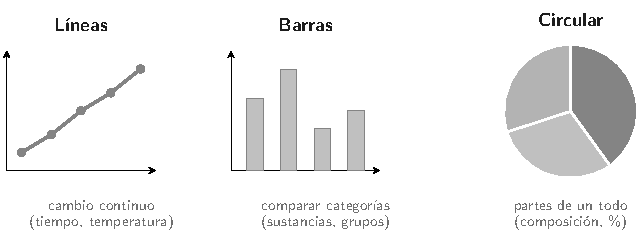
\includegraphics[max width=0.92\linewidth,max height=8.5cm]{qui/hab_graficos}
\end{center}
  
\begin{center}\small
\begin{tabularx}{\linewidth}{@{}>{\raggedright\arraybackslash\hsize=1.16\hsize}X>{\raggedright\arraybackslash\hsize=0.84\hsize}X@{}}
\toprule
\textbf{Objetivo} & \textbf{Recurso} \\
\midrule
Mostrar cómo cambia una variable continua (tiempo, temperatura, concentración) & Gráfico de líneas o de puntos \\
Comparar categorías (sustancias, marcas, métodos) & Gráfico de barras \\
Mostrar las partes de un total (composición en \%) & Gráfico circular \\
Entregar valores exactos o muchas variables & Tabla \\
Mostrar la forma de una molécula en el espacio & Modelo de esferas y varillas \\
Mostrar los grupos funcionales & Fórmula estructural \\
\bottomrule
\end{tabularx}
\end{center}
  
\begin{clave}[{Qué va en cada eje}] La variable independiente va en el eje horizontal y la dependiente en el vertical. Ejemplo: «a medida que el electrón está más lejos del núcleo, se necesita menos energía para separarlo». Eje horizontal: distancia al núcleo. Eje vertical: energía.\end{clave}
 
\begin{ojo}[{Moléculas en 3D}] Dos formas de una molécula con los mismos átomos, pero ordenados distinto en el espacio, tienen la misma fórmula molecular y la misma fórmula empírica. Para distinguirlas se necesita un modelo tridimensional, como el de esferas y varillas.\end{ojo}
 
\begin{clave}[{Tablas coherentes}] La composición porcentual de un compuesto puro es la misma en cualquier muestra: 5 g o 25 g de H\textsubscript{3}PO\textsubscript{4} tienen los mismos porcentajes de H, P y O. Una tabla que muestre porcentajes distintos para dos muestras del mismo compuesto está mal.\end{clave}
\subsection{Lo clave del tema}
\begin{center}\small
\begin{tabularx}{\linewidth}{@{}>{\raggedright\arraybackslash\hsize=0.64\hsize}X>{\raggedright\arraybackslash\hsize=1.36\hsize}X@{}}
\toprule
\textbf{Concepto} & \textbf{Pregunta que te haces} \\
\midrule
Validez & ¿El diseño permite responder la pregunta? ¿Se controlaron las variables? \\
Confiabilidad & ¿Hubo repeticiones? ¿Los instrumentos son precisos? \\
Conclusión válida & ¿Sale de los datos y no va más allá? \\
Mejora del diseño & ¿Qué defecto impide cumplir el objetivo y cómo se corrige? \\
Reproducibilidad & ¿Lo que se cambia altera una propiedad intensiva del sistema? \\
Alcance tecnológico & ¿La aplicación se limita a las condiciones estudiadas? \\
Comunicar & ¿Qué recurso muestra mejor lo que quiero mostrar? \\
\bottomrule
\end{tabularx}
\end{center}
 
\begin{clave}[{Recuerda}] · Para afirmar que un reactivo diferencia dos tipos de compuestos, hay que probarlo con ambos.\par · Los datos pueden ser correctos aunque el diseño no responda la pregunta.\par · Densidad y concentración son intensivas: no cambian con la cantidad de muestra.\par · El alcance de una conclusión se limita a condiciones similares a las estudiadas.\par · Las partes de un todo, como la composición del aire, se muestran en un gráfico circular.\end{clave}
 
\begin{clave}[{Método PAES}] 1. Escribe en una línea el objetivo de la investigación. 2. Revisa si el diseño cambia solo la variable independiente, tiene control y repeticiones. 3. Para una conclusión o un alcance, descarta lo que afirma más de lo medido. 4. Para una mejora, elige la que corrige el defecto que impide cumplir el objetivo. 5. Para comunicar, elige el recurso según lo que se quiere mostrar: cambio continuo, categorías, partes de un todo o forma en el espacio.\end{clave}
\begin{elejemplo}{PAES Invierno 2027, adaptada}
Después de ver un video sobre el mar Muerto, cuyas aguas mantienen flotando a las personas, una profesora pide a sus estudiantes encontrar, a temperatura ambiente, la concentración mínima de sal de mesa que permite que un huevo flote. Los estudiantes realizan cinco ensayos con el mismo huevo y entregan los resultados de la tabla, diciendo que lograron el objetivo. Sin embargo, la profesora les comenta que el procedimiento se puede mejorar.

¿Qué modificación les permite cumplir el objetivo?
\begin{center}\small
\begin{tabularx}{\linewidth}{@{}>{\raggedright\arraybackslash\hsize=0.47\hsize}X>{\raggedright\arraybackslash\hsize=0.79\hsize}X>{\raggedright\arraybackslash\hsize=1.89\hsize}X>{\raggedright\arraybackslash\hsize=0.84\hsize}X@{}}
\toprule
\textbf{Ensayo} & \textbf{Masa de sal (g)} & \textbf{Volumen de solución (cm\textsuperscript{3})} & \textbf{¿El huevo flota?} \\
\midrule
\textbf{1} & 6 & 200 & No \\
\textbf{2} & 9 & 300 & No \\
\textbf{3} & 12 & 400 & No \\
\textbf{4} & 15 & 500 & No \\
\textbf{5} & 60 & 1000 & Sí \\
\bottomrule
\end{tabularx}
\end{center}
\altslargas{Repetir varias veces el ensayo 5 con el mismo huevo.}{Cambiar el huevo por otro de mayor masa en cada ensayo.}{Usar un tipo de sal distinto en cada ensayo.}{Preparar soluciones con concentraciones distintas entre sí, entre 0,03 y 0,06 g/cm\textsuperscript{3}.}
\solucion{\textbf{Paso 1. ¿Qué nos piden?} Una mejora que permita encontrar la concentración \textbf{mínima} de sal con que flota el huevo. Primero hay que ver qué concentraciones se probaron.

\textbf{Paso 2. Calcula la concentración de cada ensayo} (masa de sal dividida por volumen).\par Ensayo 1: $\dfrac{6}{200} = 0{,}03$ g/cm\textsuperscript{3}.\par Ensayo 2: $\dfrac{9}{300} = 0{,}03$ g/cm\textsuperscript{3}.\par Ensayo 3: $\dfrac{12}{400} = 0{,}03$ g/cm\textsuperscript{3}.\par Ensayo 4: $\dfrac{15}{500} = 0{,}03$ g/cm\textsuperscript{3}.\par Ensayo 5: $\dfrac{60}{1000} = 0{,}06$ g/cm\textsuperscript{3}.

\textbf{Paso 3. Detecta el defecto.} Aunque las masas y los volúmenes cambian, los ensayos 1 a 4 son la \textbf{misma} concentración: 0,03 g/cm\textsuperscript{3}. La variable independiente (la concentración) casi no se varió. Solo se sabe que con 0,03 no flota y con 0,06 sí; la mínima puede ser cualquier valor entre ambas.

\textbf{Paso 4. Elige la mejora.} Hay que probar concentraciones distintas entre sí en ese intervalo, por ejemplo 0,035; 0,04; 0,045; 0,05 y 0,055 g/cm\textsuperscript{3}, manteniendo el mismo huevo y la temperatura ambiente.

\textbf{Respuesta:} preparar soluciones con concentraciones distintas entre sí, entre 0,03 y 0,06 g/cm\textsuperscript{3}.

\textbf{Comprobación:} con esta mejora, la concentración mínima quedaría entre el último ensayo en que el huevo se hunde y el primero en que flota, en un intervalo de 0,005 g/cm\textsuperscript{3} en vez de 0,03 g/cm\textsuperscript{3}.

\textbf{¿Por qué no las otras?} Repetir el ensayo 5 confirmaría que el huevo flota a 0,06 g/cm\textsuperscript{3}, pero no dice nada sobre concentraciones menores. Cambiar el huevo en cada ensayo agrega una segunda variable: si flota, no se sabría si fue por la sal o por el huevo. Lo mismo ocurre al cambiar el tipo de sal: el objetivo pide sal de mesa, y cambiarla impide comparar los ensayos.

\textbf{\color{cienciaD}Para recordar.} Antes de mejorar un diseño, calcula qué valores de la variable independiente se probaron de verdad.}{D}
\end{elejemplo}

\clearpage\renewcommand{\cabeza}{Química · Solo Mención}
\chapter{Solo Mención Química}
Este capítulo es \textbf{solo para la Mención Química}: sus temas no salen en el Módulo Común, únicamente en las 26 preguntas del Módulo Electivo. Profundiza lo de los capítulos anteriores con moléculas más complejas, isómeros y problemas de estequiometría y soluciones en varios pasos.

%% =====================================================================
%% qui_e_moleculas
\section[Moléculas complejas: insaturaciones, enlaces e hibridación (Mención)]{Moléculas complejas: insaturaciones, enlaces e hibridación}
\modmencion\ \ {\color{gris}\itshape Para el Módulo Electivo: contar los hidrógenos que no se dibujan, usar las insaturaciones (anillos + enlaces \ensuremath{\pi}) para conectar la fórmula molecular con la estructura, y contar enlaces \ensuremath{\sigma}, \ensuremath{\pi} y carbonos sp², sp o sp³ en moléculas reales con anillos y grupos funcionales.\par}
\subsection{Los hidrógenos que no se dibujan}
En el Módulo Electivo casi todas las moléculas vienen en fórmula topológica o con anillos de benceno, y los H no aparecen. Para escribir la fórmula molecular hay que \textbf{reponerlos}:

 
\begin{clave}[{Regla}] H de un carbono $= 4 -$ (enlaces que ya tiene dibujados). Un doble cuenta 2 y un triple cuenta 3.\end{clave}
 

\textbf{Ejemplo: cinamaldehído} (aroma de la canela), C\textsubscript{6}H\textsubscript{5}--CH=CH--CHO.

 
\begin{center}\small
\begin{tabular}{@{}lll@{}}
\toprule
\textbf{Parte} & \textbf{C} & \textbf{H} \\
\midrule
anillo con un sustituyente, C\textsubscript{6}H\textsubscript{5}-- & 6 & 5 \\
--CH=CH-- & 2 & 2 \\
--CHO (aldehído) & 1 & 1 \\
\textbf{Total} & \textbf{9} & \textbf{8} \\
\bottomrule
\end{tabular}
\end{center}
 

Con el O del aldehído: \textbf{C\textsubscript{9}H\textsubscript{8}O}.

  
\begin{clave}[{El anillo de benceno según sus sustituyentes}] · 1 sustituyente: C\textsubscript{6}H\textsubscript{5}-- (5 H)\par · 2 sustituyentes: --C\textsubscript{6}H\textsubscript{4}-- (4 H)\par · 3 sustituyentes: C\textsubscript{6}H\textsubscript{3} (3 H)\par Cada sustituyente le quita un H al anillo.\end{clave}
 
\begin{ojo}[{Error típico}] Contar el anillo siempre como C\textsubscript{6}H\textsubscript{6} o C\textsubscript{6}H\textsubscript{5}, aunque tenga dos o tres grupos pegados. El vértice que lleva un sustituyente no tiene H.\end{ojo}
 
\begin{ojo}[{Otro error}] Olvidar los H de los grupos: el --OH tiene 1 H, el --OCH\textsubscript{3} tiene 3, el --CHO tiene 1 y el --COOH tiene 1.\end{ojo}
\subsection{Insaturaciones: anillos y enlaces \ensuremath{\pi}}
Un alcano de cadena abierta tiene el máximo de H posible: C\textsubscript{n}H\textsubscript{2n+2}. Cada \textbf{anillo} o cada \textbf{enlace \ensuremath{\pi}} le quita 2 H. Ese «faltante» se mide con las \textbf{insaturaciones}:

 \[ I = \dfrac{2C + 2 + N - H - X}{2} \] 

C = carbonos, H = hidrógenos, N = nitrógenos, X = halógenos (F, Cl, Br, I). \textbf{El O y el S no cuentan.}

 
\begin{center}\small
\begin{tabularx}{\linewidth}{@{}>{\raggedright\arraybackslash\hsize=0.86\hsize}X>{\raggedright\arraybackslash\hsize=0.54\hsize}X>{\raggedright\arraybackslash\hsize=0.43\hsize}X>{\raggedright\arraybackslash\hsize=2.16\hsize}X@{}}
\toprule
\textbf{Compuesto} & \textbf{Fórmula} & \textbf{$I$} & \textbf{Qué significa} \\
\midrule
hexano & C\textsubscript{6}H\textsubscript{14} & 0 & solo simples, sin anillo \\
hex-1-eno & C\textsubscript{6}H\textsubscript{12} & 1 & un doble \\
ciclohexano & C\textsubscript{6}H\textsubscript{12} & 1 & un anillo \\
benceno & C\textsubscript{6}H\textsubscript{6} & 4 & 1 anillo + 3 dobles \\
cinamaldehído & C\textsubscript{9}H\textsubscript{8}O & 6 & 1 anillo + 3 dobles del anillo + 1 C=C + 1 C=O \\
\bottomrule
\end{tabularx}
\end{center}
  
\begin{clave}[{Cuánto vale cada cosa}] Anillo: 1. Doble (C=C, C=O o C=N): 1. Triple: 2. Un anillo de benceno completo: 4.\end{clave}
 
\begin{ejemplo}[{Ejemplo resuelto}] C\textsubscript{9}H\textsubscript{8}O: $I = \dfrac{2\cdot 9 + 2 - 8}{2} = \dfrac{12}{2} = 6$. El benceno aporta 4; quedan 2: un C=C y un C=O. \ding{52} Coincide con C\textsubscript{6}H\textsubscript{5}--CH=CH--CHO.\end{ejemplo}
 
\begin{ojo}[{Error típico}] Restar el O en la fórmula. El oxígeno forma 2 enlaces y se «intercala» sin cambiar el número de H: el etanol C\textsubscript{2}H\textsubscript{6}O tiene $I = 0$, igual que el etano C\textsubscript{2}H\textsubscript{6}.\end{ojo}
\subsection{De la fórmula a la estructura (y al revés)}
Cuando te dan una fórmula molecular y cuatro estructuras posibles, las insaturaciones descartan opciones en segundos.

 

\textbf{Ejemplo.} ¿Qué estructura corresponde a C\textsubscript{4}H\textsubscript{8}O\textsubscript{2}?

 

\textbf{Paso 1.} $I = \dfrac{2\cdot 4 + 2 - 8}{2} = 1$: la estructura tiene \textbf{un} doble enlace (C=C o C=O) \textbf{o} un anillo.

 

\textbf{Paso 2.} Revisa cada opción:

 
\begin{center}\small
\begin{tabular}{@{}lll@{}}
\toprule
\textbf{Estructura} & \textbf{Fórmula} & \textbf{¿Sirve?} \\
\midrule
CH\textsubscript{3}--CH\textsubscript{2}--CH\textsubscript{2}--COOH (ácido butanoico) & C\textsubscript{4}H\textsubscript{8}O\textsubscript{2} & \ding{52} \\
CH\textsubscript{3}--COO--CH\textsubscript{2}--CH\textsubscript{3} (etanoato de etilo) & C\textsubscript{4}H\textsubscript{8}O\textsubscript{2} & \ding{52} \\
HO--CH\textsubscript{2}--CH\textsubscript{2}--CH\textsubscript{2}--CH\textsubscript{2}--OH & C\textsubscript{4}H\textsubscript{10}O\textsubscript{2} & \ding{56} ($I = 0$) \\
CH\textsubscript{3}--CO--CO--CH\textsubscript{3} & C\textsubscript{4}H\textsubscript{6}O\textsubscript{2} & \ding{56} ($I = 2$) \\
\bottomrule
\end{tabular}
\end{center}
  
\begin{clave}[{Pistas que da el enunciado}] «Tiene un anillo aromático» = 4 insaturaciones. «Es un aldehído, cetona, ácido o éster» = un C=O, 1 insaturación. «Tiene n dobles C=C» = n insaturaciones. Suma todo y compara con la fórmula.\end{clave}
 
\begin{ojo}[{Ojo con «dobles C--C»}] En la PAES, al contar dobles enlaces C=C de un compuesto con benceno, se cuentan los 3 del anillo dibujado. Si te dicen «4 dobles C=C» y hay un anillo, el cuarto está en la cadena.\end{ojo}
\subsection{Contar \ensuremath{\sigma} y \ensuremath{\pi} en moléculas con anillos}
Dos atajos sirven para cualquier molécula, por grande que sea:

 
\begin{clave}[{Enlaces \ensuremath{\sigma}}] $\sigma = \text{átomos} - 1 + \text{anillos}$\end{clave}
 
\begin{clave}[{Enlaces \ensuremath{\pi}}] $\pi = I - \text{anillos}$ (1 por cada doble, 2 por cada triple)\end{clave}
 
\begin{center}\small
\begin{tabular}{@{}llllll@{}}
\toprule
\textbf{Molécula} & \textbf{Átomos} & \textbf{Anillos} & \textbf{$\sigma$} & \textbf{$\pi$} & \textbf{$\sigma : \pi$} \\
\midrule
propeno, C\textsubscript{3}H\textsubscript{6} & 9 & 0 & 8 & 1 & 8 : 1 \\
propino, C\textsubscript{3}H\textsubscript{4} & 7 & 0 & 6 & 2 & 3 : 1 \\
benceno, C\textsubscript{6}H\textsubscript{6} & 12 & 1 & 12 & 3 & 4 : 1 \\
ciclohexeno, C\textsubscript{6}H\textsubscript{10} & 16 & 1 & 16 & 1 & 16 : 1 \\
\bottomrule
\end{tabular}
\end{center}
  
\begin{ejemplo}[{Ejemplo resuelto}] ¿Cuántos $\sigma$ y $\pi$ tiene el tolueno, C\textsubscript{6}H\textsubscript{5}--CH\textsubscript{3}?\par \textbf{Paso 1.} Fórmula: C\textsubscript{7}H\textsubscript{8}, 15 átomos, 1 anillo.\par \textbf{Paso 2.} $\sigma = 15 - 1 + 1 = 15$.\par \textbf{Paso 3.} $I = \dfrac{14 + 2 - 8}{2} = 4$; $\pi = 4 - 1 = 3$.\par \textbf{Comprobación:} 7 enlaces C--C (6 del anillo + 1 al CH\textsubscript{3}) + 8 C--H = 15 $\sigma$. \ding{52}\end{ejemplo}
 
\begin{ojo}[{Error típico}] Olvidar sumar el anillo. En una cadena abierta hay un enlace menos que átomos; al cerrar el anillo se agrega un enlace más.\end{ojo}
\subsection{Hibridación en moléculas reales}
Para contar carbonos sp\textsuperscript{2}, sp o sp\textsuperscript{3} en una molécula grande, recorre \textbf{los enlaces múltiples}: cada doble C=C «pinta» de sp\textsuperscript{2} a sus \textbf{dos} carbonos; cada C=O pinta de sp\textsuperscript{2} a su carbono; cada triple pinta de sp a sus dos carbonos. Los carbonos que quedan sin pintar son sp\textsuperscript{3}.

 

\textbf{Ejemplo: limoneno} (C\textsubscript{10}H\textsubscript{16}, olor a cítricos). Tiene un anillo de seis carbonos con un C=C, y un grupo --C(CH\textsubscript{3})=CH\textsubscript{2}.

 

Dobles: 2 \ensuremath{\rightarrow} carbonos sp\textsuperscript{2}: $2\cdot 2 = 4$. Los otros 6 son sp\textsuperscript{3}.

 
\begin{center}\small
\begin{tabular}{@{}ll@{}}
\toprule
\textbf{Grupo} & \textbf{Carbonos y su hibridación} \\
\midrule
anillo de benceno & los 6 C son sp\textsuperscript{2} \\
--CHO, --CO--, --COOH, --COO--, --CONH\textsubscript{2} & el C del C=O es sp\textsuperscript{2} \\
--C\ensuremath{\equiv}N, --C\ensuremath{\equiv}C-- & sp \\
--CH\textsubscript{3}, --CH\textsubscript{2}--, C con OH o con O de éter & sp\textsuperscript{3} (si no tiene dobles) \\
\bottomrule
\end{tabular}
\end{center}
  
\begin{ejemplo}[{Ejemplo resuelto}] Estireno, C\textsubscript{6}H\textsubscript{5}--CH=CH\textsubscript{2}: anillo (6 sp\textsuperscript{2}) + C=C de la cadena (2 sp\textsuperscript{2}) = \textbf{8 carbonos sp\textsuperscript{2}}, ninguno sp\textsuperscript{3}. Fórmula C\textsubscript{8}H\textsubscript{8}.\end{ejemplo}
 
\begin{ojo}[{Error típico}] Contar enlaces \ensuremath{\pi} en vez de carbonos. El limoneno tiene 2 enlaces \ensuremath{\pi} pero 4 carbonos sp\textsuperscript{2}: cada doble involucra a dos carbonos.\end{ojo}
 
\begin{ojo}[{Otro error}] Decir que el C de un --COOH es sp\textsuperscript{3} porque tiene un OH. Mira todos sus enlaces: tiene un C=O, así que es sp\textsuperscript{2}.\end{ojo}
\subsection{Lo clave del tema}
\begin{center}\small
\begin{tabularx}{\linewidth}{@{}>{\raggedright\arraybackslash\hsize=0.53\hsize}X>{\raggedright\arraybackslash\hsize=1.24\hsize}X>{\raggedright\arraybackslash\hsize=1.24\hsize}X@{}}
\toprule
\textbf{Herramienta} & \textbf{Fórmula o regla} & \textbf{Para qué sirve} \\
\midrule
H implícitos & H = 4 \ensuremath{-} enlaces dibujados del C & pasar de topológica a fórmula molecular \\
Insaturaciones & $I = \dfrac{2C + 2 + N - H - X}{2}$ (sin O ni S) & saber cuántos anillos + \ensuremath{\pi} hay; descartar estructuras \\
Enlaces \ensuremath{\sigma} & átomos \ensuremath{-} 1 + anillos & contar \ensuremath{\sigma} sin dibujar todos los H \\
Enlaces \ensuremath{\pi} & $I$ \ensuremath{-} anillos & contar \ensuremath{\pi} de una vez \\
Hibridación & doble \ensuremath{\rightarrow} sus 2 C son sp²; triple \ensuremath{\rightarrow} sus 2 C son sp; el resto sp³ & contar carbonos de cada tipo \\
\bottomrule
\end{tabularx}
\end{center}
  
\begin{clave}[{Recuerda}] · Benceno = 4 insaturaciones (1 anillo + 3 \ensuremath{\pi}).\par · Cada sustituyente le quita un H al anillo: C\textsubscript{6}H\textsubscript{5}--, --C\textsubscript{6}H\textsubscript{4}--.\par · Propino: 6 $\sigma$ y 2 $\pi$, razón 3 : 1.\par · Limoneno: 2 dobles, 4 carbonos sp\textsuperscript{2}.\end{clave}
  
\begin{clave}[{Método PAES}] 1. Calcula la fórmula molecular de cada opción (repón los H). 2. Calcula $I$ y compáralo con lo que pide el enunciado. 3. Para $\sigma$ y $\pi$ usa los atajos y comprueba contando un tipo de enlace. 4. Para hibridación, recorre los enlaces múltiples.\end{clave}
\begin{elejemplo}{PAES Invierno 2027, adaptada}
El aceite esencial de anís contiene un compuesto X de fórmula molecular C\textsubscript{10}H\textsubscript{12}O. Mediante análisis químicos se determinó que la molécula X:

· tiene un grupo metoxi (--O--CH\textsubscript{3}) unido a un anillo de benceno;\par · tiene, unida al mismo anillo, una cadena de 3 átomos de carbono con un doble enlace.

¿Cuál de las siguientes estructuras es coherente con esta información?
\alts{CH\textsubscript{3}O--C\textsubscript{6}H\textsubscript{4}--CH\textsubscript{2}--CH\textsubscript{2}--CH\textsubscript{3}}{HO--C\textsubscript{6}H\textsubscript{4}--CH=CH--CH\textsubscript{3}}{CH\textsubscript{3}O--C\textsubscript{6}H\textsubscript{4}--CH=CH--CH\textsubscript{3}}{CH\textsubscript{3}O--C\textsubscript{6}H\textsubscript{4}--C\ensuremath{\equiv}C--CH\textsubscript{3}}
\solucion{\textbf{Paso 1. ¿Qué nos piden?} La estructura que cumple las dos características y además tiene la fórmula C\textsubscript{10}H\textsubscript{12}O.

\textbf{Paso 2. Insaturaciones de la fórmula.} $I = \dfrac{2\cdot 10 + 2 - 12}{2} = \dfrac{10}{2} = 5$. El benceno aporta 4: queda \textbf{1}, justo un doble enlace en la cadena. \ding{52} Coincide con la descripción.

\textbf{Paso 3. Revisa la opción CH\textsubscript{3}O--C\textsubscript{6}H\textsubscript{4}--CH=CH--CH\textsubscript{3}.} Tiene metoxi y una cadena de 3 C con un doble. C: $1 + 6 + 3 = 10$. H: $3 + 4 + 1 + 1 + 3 = 12$. O: 1. Fórmula C\textsubscript{10}H\textsubscript{12}O. \ding{52}

\textbf{Respuesta:} CH\textsubscript{3}O--C\textsubscript{6}H\textsubscript{4}--CH=CH--CH\textsubscript{3} (el anetol).

\textbf{Comprobación:} anillo (4) + un C=C (1) = 5 insaturaciones, las mismas que da la fórmula. \ding{52}

\textbf{¿Por qué no las otras?} La de cadena --CH\textsubscript{2}--CH\textsubscript{2}--CH\textsubscript{3} no tiene doble enlace: es C\textsubscript{10}H\textsubscript{14}O, con 4 insaturaciones. La que tiene HO-- es un fenol, no un éter metílico: le falta un carbono y es C\textsubscript{9}H\textsubscript{10}O. La del triple tiene 2 insaturaciones en la cadena: es C\textsubscript{10}H\textsubscript{10}O.

\textbf{\color{cienciaD}Para recordar.} Calcula las insaturaciones de la fórmula, réstale 4 por el benceno y lo que queda te dice cuántos dobles hay en la cadena.}{C}
\end{elejemplo}

%% =====================================================================
%% qui_e_isomeros
\section[Isómeros y propiedades físicas de compuestos orgánicos (Mención)]{Isómeros y propiedades físicas de compuestos orgánicos}
\modmencion\ \ {\color{gris}\itshape Para el Módulo Electivo: reconocer isómeros de cadena, de posición, de función y geométricos (cis y trans), saber qué representación los distingue, y predecir la temperatura de ebullición y la solubilidad en agua según el largo de la cadena, la ramificación y el grupo funcional.\par}
\subsection{Misma fórmula, distinta estructura}
Dos compuestos son \textbf{isómeros} si tienen la \textbf{misma fórmula molecular} (y por eso la misma masa molar) pero \textbf{distinta estructura}. Son sustancias distintas, con propiedades distintas.

 
\begin{center}\small
\begin{tabularx}{\linewidth}{@{}>{\raggedright\arraybackslash\hsize=0.50\hsize}X>{\raggedright\arraybackslash\hsize=1.32\hsize}X>{\raggedright\arraybackslash\hsize=1.18\hsize}X@{}}
\toprule
\textbf{Tipo} & \textbf{Qué cambia} & \textbf{Ejemplo} \\
\midrule
De cadena & el esqueleto de carbonos & pentano y 2-metilbutano (C\textsubscript{5}H\textsubscript{12}) \\
De posición & dónde está el grupo o el doble enlace & propan-1-ol y propan-2-ol (C\textsubscript{3}H\textsubscript{8}O) \\
De función & el grupo funcional & etanol y metoximetano (C\textsubscript{2}H\textsubscript{6}O) \\
Geométricos & la disposición en el espacio & cis- y trans-but-2-eno (C\textsubscript{4}H\textsubscript{8}) \\
\bottomrule
\end{tabularx}
\end{center}
  
\begin{clave}[{Cómo comprobar}] 1. Escribe la fórmula molecular de cada uno. 2. Si son distintas, \textbf{no} son isómeros. 3. Si son iguales, mira qué cambió: cadena, posición, función o espacio.\end{clave}
 
\begin{ojo}[{Error típico}] Llamar isómeros a dos dibujos del mismo compuesto. CH\textsubscript{3}--CH\textsubscript{2}--CH\textsubscript{2}--CH\textsubscript{3} dibujado recto o «doblado» sigue siendo butano: si al nombrarlos sale el mismo nombre, es la misma sustancia.\end{ojo}
 
\begin{ojo}[{Otro error}] Llamar isómeros a compuestos de la misma familia con distinto número de C. Etanol (C\textsubscript{2}H\textsubscript{6}O) y propan-1-ol (C\textsubscript{3}H\textsubscript{8}O) no son isómeros: son de la misma serie homóloga.\end{ojo}
\subsection{Isómeros de función: las parejas que se repiten}
Las insaturaciones explican por qué ciertas familias comparten fórmula general:

 
\begin{center}\small
\begin{tabularx}{\linewidth}{@{}>{\raggedright\arraybackslash\hsize=0.56\hsize}X>{\raggedright\arraybackslash\hsize=0.94\hsize}X>{\raggedright\arraybackslash\hsize=1.50\hsize}X@{}}
\toprule
\textbf{Fórmula general} & \textbf{Pareja de familias} & \textbf{Ejemplo} \\
\midrule
C\textsubscript{n}H\textsubscript{2n+2}O & alcohol \ensuremath{\leftrightarrow} éter & butan-1-ol y etoxietano (C\textsubscript{4}H\textsubscript{10}O) \\
C\textsubscript{n}H\textsubscript{2n}O & aldehído \ensuremath{\leftrightarrow} cetona & propanal y propanona (C\textsubscript{3}H\textsubscript{6}O) \\
C\textsubscript{n}H\textsubscript{2n}O\textsubscript{2} & ácido carboxílico \ensuremath{\leftrightarrow} éster & ácido propanoico y etanoato de metilo (C\textsubscript{3}H\textsubscript{6}O\textsubscript{2}) \\
C\textsubscript{n}H\textsubscript{2n} & alqueno \ensuremath{\leftrightarrow} cicloalcano & hex-1-eno y ciclohexano (C\textsubscript{6}H\textsubscript{12}) \\
C\textsubscript{n}H\textsubscript{2n\ensuremath{-}2} & alquino \ensuremath{\leftrightarrow} dieno & but-1-ino y buta-1,3-dieno (C\textsubscript{4}H\textsubscript{6}) \\
\bottomrule
\end{tabularx}
\end{center}
  
\begin{ejemplo}[{Ejemplo resuelto}] ¿Es el etanoato de metilo, CH\textsubscript{3}--COO--CH\textsubscript{3}, isómero del ácido propanoico, CH\textsubscript{3}--CH\textsubscript{2}--COOH?\par \textbf{Paso 1.} Etanoato de metilo: C = 3, H = $3 + 3 = 6$, O = 2.\par \textbf{Paso 2.} Ácido propanoico: C = 3, H = $3 + 2 + 1 = 6$, O = 2.\par \textbf{Paso 3.} Misma fórmula, C\textsubscript{3}H\textsubscript{6}O\textsubscript{2}, y distinto grupo funcional: \textbf{isómeros de función}.\end{ejemplo}
 
\begin{ojo}[{Ojo}] Los isómeros tienen la misma masa molar, pero eso no basta: dos compuestos pueden tener igual masa molar con fórmulas distintas (el propan-1-ol, C\textsubscript{3}H\textsubscript{8}O, y el ácido acético, C\textsubscript{2}H\textsubscript{4}O\textsubscript{2}, pesan 60 g/mol).\end{ojo}
\subsection{Isómeros geométricos: cis y trans}
Un doble enlace C=C \textbf{no puede girar}: el enlace $\pi$ lo traba. Si cada carbono del doble tiene dos grupos \textbf{distintos}, hay dos formas de ordenarlos:

 
\begin{itemize}
  \item \textbf{cis}: los grupos iguales quedan del \textbf{mismo lado} del doble enlace.
  \item \textbf{trans}: quedan en lados \textbf{opuestos}.
\end{itemize}
 
\begin{center}\small
\begin{tabularx}{\linewidth}{@{}>{\raggedright\arraybackslash\hsize=1.22\hsize}X>{\raggedright\arraybackslash\hsize=0.65\hsize}X>{\raggedright\arraybackslash\hsize=1.14\hsize}X@{}}
\toprule
\textbf{Compuesto} & \textbf{¿Tiene cis/trans?} & \textbf{Por qué} \\
\midrule
but-2-eno, CH\textsubscript{3}--CH=CH--CH\textsubscript{3} & sí & cada C del doble tiene H y CH\textsubscript{3} \\
but-1-eno, CH\textsubscript{2}=CH--CH\textsubscript{2}--CH\textsubscript{3} & no & el C1 tiene dos H iguales \\
2-metilbut-2-eno, (CH\textsubscript{3})\textsubscript{2}C=CH--CH\textsubscript{3} & no & el C2 tiene dos CH\textsubscript{3} iguales \\
1,2-dicloroeteno, CHCl=CHCl & sí & cada C tiene H y Cl \\
\bottomrule
\end{tabularx}
\end{center}
  
\begin{clave}[{¿Qué representación los distingue?}] La fórmula molecular, la empírica, la condensada y la semidesarrollada son \textbf{iguales} para el cis y el trans (CH\textsubscript{3}--CH=CH--CH\textsubscript{3} en ambos). Solo una representación que muestre el espacio los separa: el \textbf{modelo de esferas y varillas}, el modelo compacto o una fórmula desarrollada dibujada con los ángulos.\end{clave}
 
\begin{clave}[{Propiedades distintas}] cis-1,2-dicloroeteno: ebulle a 60 °C. trans-1,2-dicloroeteno: ebulle a 48 °C. En los fármacos, dos formas que solo difieren en el espacio pueden tener efectos biológicos muy distintos.\end{clave}
\subsection{Temperatura de ebullición: tamaño y forma}
Para hervir, las moléculas deben separarse de sus vecinas. Mientras más se atraen, más alta es la temperatura de ebullición. En los hidrocarburos la atracción depende de la \textbf{superficie de contacto}:

 
\begin{clave}[{Regla 1. Largo de cadena}] En una serie de alcanos lineales, a más carbonos, mayor temperatura de ebullición.\end{clave}
 
\begin{clave}[{Regla 2. Ramificación}] Entre isómeros, a más ramificación, la molécula es más compacta (más «esférica»), toca menos a sus vecinas y hierve a menor temperatura.\end{clave}
  
\begin{center}\small
\begin{tabular}{@{}lll@{}}
\toprule
\textbf{Isómero} & \textbf{Fórmula} & \textbf{T. de ebullición (°C)} \\
\midrule
pentano & C\textsubscript{5}H\textsubscript{12} & 36,1 \\
2-metilbutano & C\textsubscript{5}H\textsubscript{12} & 27,8 \\
2,2-dimetilpropano & C\textsubscript{5}H\textsubscript{12} & 9,5 \\
hexano & C\textsubscript{6}H\textsubscript{14} & 68,7 \\
2-metilpentano & C\textsubscript{6}H\textsubscript{14} & 60,3 \\
2,2-dimetilbutano & C\textsubscript{6}H\textsubscript{14} & 49,7 \\
\bottomrule
\end{tabular}
\end{center}
 
\begin{ojo}[{Para predecir con una tabla}] Ubica la molécula nueva entre las conocidas: mismo número de C que una fila y ramificación intermedia \ensuremath{\rightarrow} temperatura intermedia. Nunca puede pasar al isómero lineal ni quedar bajo el más ramificado de su grupo.\end{ojo}
\subsection{Temperatura de ebullición: el grupo funcional}
Con masas molares parecidas, lo que decide es el \textbf{grupo funcional}:

 
\begin{center}\small
\begin{tabular}{@{}llll@{}}
\toprule
\textbf{Compuesto} & \textbf{Familia} & \textbf{M (g/mol)} & \textbf{T. eb. (°C)} \\
\midrule
butano & alcano & 58 & \ensuremath{-}0,5 \\
metoxietano & éter & 60 & 7 \\
propanal & aldehído & 58 & 48 \\
propanona & cetona & 58 & 56 \\
propan-1-ol & alcohol & 60 & 97 \\
ácido etanoico & ácido carboxílico & 60 & 118 \\
\bottomrule
\end{tabular}
\end{center}
  
\begin{clave}[{Por qué}] Los grupos --OH (alcoholes y ácidos) y --NH forman \textbf{puentes de hidrógeno} entre moléculas: la atracción más fuerte. El C=O de aldehídos y cetonas es polar, pero no forma puentes de hidrógeno entre sus moléculas. Éteres y alcanos casi no tienen polaridad.\end{clave}
 
\begin{clave}[{Más grupos --OH, más alta}] propan-1-ol 97 °C; propano-1,2-diol 188 °C; propano-1,2,3-triol (glicerina) 290 °C.\end{clave}
 
\begin{clave}[{Solubilidad en agua}] «Lo semejante disuelve a lo semejante». Los alcoholes y ácidos pequeños se mezclan con el agua por sus puentes de hidrógeno; los hidrocarburos no. Al alargar la cadena (parte apolar) la solubilidad baja: el metanol se mezcla en cualquier proporción y el pentan-1-ol apenas se disuelve (unos 2 g por 100 mL).\end{clave}
\subsection{Lo clave del tema}
\begin{center}\small
\begin{tabularx}{\linewidth}{@{}>{\raggedright\arraybackslash\hsize=0.71\hsize}X>{\raggedright\arraybackslash\hsize=1.29\hsize}X@{}}
\toprule
\textbf{Pregunta} & \textbf{Cómo responderla} \\
\midrule
¿Son isómeros? & misma fórmula molecular y distinta estructura \\
¿De qué tipo? & cadena (esqueleto), posición (lugar del grupo), función (grupo distinto), geométrico (cis/trans) \\
¿Tiene cis/trans? & doble C=C con dos grupos distintos en cada carbono \\
¿Qué los distingue? & cis/trans: modelo de esferas y varillas o compacto; nunca la fórmula molecular \\
¿Cuál hierve más alto? & 1.º grupo funcional (ácido > alcohol > cetona/aldehído > éter > alcano); 2.º más C; 3.º menos ramificado \\
\bottomrule
\end{tabularx}
\end{center}
  
\begin{clave}[{Recuerda}] · Etanol (78 °C) y metoximetano (\ensuremath{-}24 °C) son isómeros: misma masa molar, ebullición muy distinta.\par · Pentano 36,1 °C > 2-metilbutano 27,8 °C > 2,2-dimetilpropano 9,5 °C.\par · Más grupos --OH, más alta la ebullición y más soluble en agua.\end{clave}
  
\begin{clave}[{Método PAES}] 1. Escribe la fórmula molecular de cada compuesto. 2. Agrupa por grupo funcional. 3. Dentro de cada grupo, ordena por número de C y luego por ramificación. 4. Si la pregunta trae tabla, ubica el compuesto nuevo entre los datos conocidos.\end{clave}
\begin{elejemplo}{PAES Invierno 2026, adaptada}
Durante la clase de química orgánica, cuatro estudiantes analizan los siguientes compuestos:

X: CH\textsubscript{3}--CH\textsubscript{2}--CH\textsubscript{2}--CH\textsubscript{2}--OH\par Y: CH\textsubscript{3}--CH\textsubscript{2}--O--CH\textsubscript{2}--CH\textsubscript{3}\par Z: CH\textsubscript{3}--CH\textsubscript{2}--CH\textsubscript{2}--COOH

Luego, cada estudiante escribe en su cuaderno:

Estudiante 1: X e Y son isómeros de posición.\par Estudiante 2: X e Y tienen la misma masa molar, y X tiene mayor temperatura de ebullición que Y.\par Estudiante 3: Z tiene más átomos de carbono que X.\par Estudiante 4: X y Z son isómeros de función.

¿Cuál de los estudiantes escribe una conclusión correcta?
\alts{El estudiante 1.}{El estudiante 2.}{El estudiante 3.}{El estudiante 4.}
\solucion{\textbf{Paso 1. ¿Qué nos piden?} Revisar cada afirmación. Primero, la fórmula molecular de cada compuesto.

\textbf{Paso 2. Fórmulas.} X (butan-1-ol): C\textsubscript{4}H\textsubscript{10}O, 74 g/mol. Y (etoxietano): C\textsubscript{4}H\textsubscript{10}O, 74 g/mol. Z (ácido butanoico): C\textsubscript{4}H\textsubscript{8}O\textsubscript{2}, 88 g/mol.

\textbf{Paso 3. Estudiante 2.} X e Y tienen la misma fórmula, así que la misma masa molar. X es un alcohol: forma puentes de hidrógeno entre sus moléculas y hierve más alto (118 °C) que el éter Y (35 °C). \textbf{Correcta.}

\textbf{Respuesta:} el estudiante 2.

\textbf{¿Por qué no las otras?} Estudiante 1: X e Y sí son isómeros, pero de \textbf{función} (alcohol y éter), no de posición. Estudiante 3: los dos tienen 4 C. Estudiante 4: X y Z tienen fórmulas distintas (C\textsubscript{4}H\textsubscript{10}O y C\textsubscript{4}H\textsubscript{8}O\textsubscript{2}), así que no son isómeros.

\textbf{\color{cienciaD}Para recordar.} Primero las fórmulas moleculares: deciden quién es isómero de quién; después el grupo funcional decide quién hierve más alto.}{B}
\end{elejemplo}

%% =====================================================================
%% qui_e_estequiometria
\section[Estequiometría a fondo: datos experimentales y masa total (Mención)]{Estequiometría a fondo: datos experimentales y masa total}
\modmencion\ \ {\color{gris}\itshape Para el Módulo Electivo: deducir la razón molar de una reacción a partir de masas medidas, balancear y calcular las cantidades de todas las sustancias de una vez, usar la conservación de la masa total, resolver el reactivo limitante cuando el dato es el producto y obtener la fórmula empírica a partir de una combustión.\par}
\subsection{De los datos a la razón molar}
En el Módulo Electivo a veces no te dan la ecuación: te dan \textbf{masas medidas} y debes descubrir en qué proporción reaccionan las sustancias.

 

\textbf{Ejemplo.} Y (27 g/mol) reacciona con un exceso de Z (32 g/mol) y forma un único producto X (102 g/mol). Con 13,5 g de Y se obtienen 25,5 g de X.

 

\textbf{Paso 1. Mol de Y y de X.} $n_Y = \dfrac{13{,}5}{27} = 0{,}5$ mol; $n_X = \dfrac{25{,}5}{102} = 0{,}25$ mol.

 

\textbf{Paso 2. Masa de Z (Lavoisier).} $25{,}5 - 13{,}5 = 12$ g, o sea $\dfrac{12}{32} = 0{,}375$ mol.

 

\textbf{Paso 3. Divide por el menor.} $0{,}5 : 0{,}375 : 0{,}25 = 2 : 1{,}5 : 1$. Multiplica por 2 para tener enteros: \textbf{4 Y + 3 Z \ensuremath{\rightarrow} 2 X}.

  
\begin{clave}[{Es la reacción}] 4 Al + 3 O\textsubscript{2} \ensuremath{\rightarrow} 2 Al\textsubscript{2}O\textsubscript{3}: Al = 27, O\textsubscript{2} = 32 y Al\textsubscript{2}O\textsubscript{3} = 102 g/mol.\end{clave}
 
\begin{clave}[{Con varias experiencias}] Si duplicas la masa de Y y el producto también se duplica, la razón es la misma: basta con calcular una fila completa y comprobar con otra.\end{clave}
 
\begin{ojo}[{Error típico}] Comparar gramos en vez de mol: «13,5 g de Y dan 25,5 g de X, casi el doble, entonces 1 Y forma 2 X». La razón molar sale de los \textbf{mol}, y aquí es al revés: 2 mol de Y forman 1 mol de X.\end{ojo}
\subsection{Todas las cantidades de una vez}
Con la ecuación balanceada puedes escribir una \textbf{fila de mol} y otra de \textbf{masas} para todas las sustancias. Combustión de la glucosa:

 
\begin{center}
C\textsubscript{6}H\textsubscript{12}O\textsubscript{6} + 6 O\textsubscript{2} \ensuremath{\rightarrow} 6 CO\textsubscript{2} + 6 H\textsubscript{2}O
\end{center}
 
\begin{center}\small
\begin{tabular}{@{}lllll@{}}
\toprule
 & \textbf{C\textsubscript{6}H\textsubscript{12}O\textsubscript{6}} & \textbf{O\textsubscript{2}} & \textbf{CO\textsubscript{2}} & \textbf{H\textsubscript{2}O} \\
\midrule
mol & 1 & 6 & 6 & 6 \\
masa (g) & 180 & $6\cdot 32 = 192$ & $6\cdot 44 = 264$ & $6\cdot 18 = 108$ \\
\bottomrule
\end{tabular}
\end{center}
 

Reactivos: $180 + 192 = 372$ g. Productos: $264 + 108 = 372$ g. \ding{52}

  
\begin{clave}[{Para qué sirve}] Si te dicen «se obtienen 372 g de productos», ya sabes que reaccionó 1 mol de glucosa con 6 mol de O\textsubscript{2} y se formaron 6 mol de CO\textsubscript{2} y 6 mol de H\textsubscript{2}O. Si te dan la mitad, todo se divide por 2.\end{clave}
 
\begin{ojo}[{Ojo}] La masa total se conserva, los mol no siempre. En N\textsubscript{2} + 3 H\textsubscript{2} \ensuremath{\rightarrow} 2 NH\textsubscript{3} entran 4 mol y salen 2, pero entran $28 + 6 = 34$ g y salen $2\cdot 17 = 34$ g.\end{ojo}
 
\begin{ojo}[{Si la ecuación no viene balanceada}] Balancéala primero. La PAES puede dar «C\textsubscript{6}H\textsubscript{12}O\textsubscript{6} + O\textsubscript{2} \ensuremath{\rightarrow} CO\textsubscript{2} + H\textsubscript{2}O» sin coeficientes justamente para ver si lo haces.\end{ojo}
\subsection{Limitante cuando el dato es el producto}
A veces el enunciado da las cantidades iniciales \textbf{y} la cantidad de producto obtenida, y pregunta cuánto se consumió de un reactivo.

 

\textbf{Ejemplo.} 2 Fe + 6 HCl \ensuremath{\rightarrow} 2 FeCl\textsubscript{3} + 3 H\textsubscript{2}. Se usan 0,1 mol de HCl y 0,1 mol de Fe, y se obtienen 0,05 mol de H\textsubscript{2}. ¿Cuánto Fe se consumió?

 

\textbf{Paso 1. Limitante.} Fe: $\dfrac{0{,}1}{2} = 0{,}05$. HCl: $\dfrac{0{,}1}{6} \approx 0{,}017$. Limita el HCl.

 

\textbf{Paso 2. Confirma con el producto.} $0{,}1\cdot\dfrac{3}{6} = 0{,}05$ mol de H\textsubscript{2}. \ding{52} Coincide con el dato.

 

\textbf{Paso 3. Fe consumido.} $0{,}1\cdot\dfrac{2}{6} \approx 0{,}03$ mol. Sobran unos 0,07 mol de Fe.

  
\gatotip[\gatogris]{\textbf{Atajo.} Si conoces el producto formado, úsalo directamente: $0{,}05$ mol de H\textsubscript{2} $\cdot\dfrac{2}{3} \approx 0{,}03$ mol de Fe. Lo que reaccionó siempre está en proporción con lo que se formó.}
 
\begin{ojo}[{Error típico}] Responder 0,1 mol de Fe, «porque se usaron 0,1 mol». Se \textbf{pusieron} 0,1 mol; se \textbf{consumió} solo lo que alcanzó a reaccionar con el HCl.\end{ojo}
\subsection{Fórmula empírica por combustión}
Al quemar un compuesto orgánico, \textbf{todo su C termina en CO\textsubscript{2}} y \textbf{todo su H termina en H\textsubscript{2}O}. Midiendo esas masas se obtiene su composición.

 

\textbf{Ejemplo.} Se queman 2,3 g de un compuesto de C, H y O y se obtienen 4,4 g de CO\textsubscript{2} y 2,7 g de H\textsubscript{2}O.

 

\textbf{Paso 1. Carbono.} En 44 g de CO\textsubscript{2} hay 12 g de C: $4{,}4\cdot\dfrac{12}{44} = 1{,}2$ g de C.

 

\textbf{Paso 2. Hidrógeno.} En 18 g de H\textsubscript{2}O hay 2 g de H: $2{,}7\cdot\dfrac{2}{18} = 0{,}3$ g de H.

 

\textbf{Paso 3. Oxígeno, por diferencia.} $2{,}3 - 1{,}2 - 0{,}3 = 0{,}8$ g de O.

 

\textbf{Paso 4. Mol y razón.} C: $\dfrac{1{,}2}{12} = 0{,}1$; H: $\dfrac{0{,}3}{1} = 0{,}3$; O: $\dfrac{0{,}8}{16} = 0{,}05$. Dividiendo por 0,05: \textbf{C\textsubscript{2}H\textsubscript{6}O}.

  
\begin{ojo}[{Error típico}] Calcular el O desde el CO\textsubscript{2} o el H\textsubscript{2}O. Ese oxígeno viene en parte del O\textsubscript{2} del aire: el O del compuesto se obtiene \textbf{restando} C y H a la masa de la muestra.\end{ojo}
 
\begin{clave}[{Si es un hidrocarburo}] Solo hay C e H: no hay que restar nada. Y si te dan la masa molar, divide por la masa de la fórmula empírica para obtener la molecular.\end{clave}
 
\begin{clave}[{Porcentaje de C}] $\%\text{C} = \dfrac{\text{masa de C}}{\text{masa de muestra}}\cdot 100$. En el ejemplo: $\dfrac{1{,}2}{2{,}3}\cdot 100 \approx 52\%$.\end{clave}
\subsection{Balancear y calcular en un solo problema}
Muchos problemas del Electivo mezclan los pasos: la ecuación viene sin balancear y te piden una masa.

 

\textbf{Ejemplo.} Fe\textsubscript{2}O\textsubscript{3} + CO \ensuremath{\rightarrow} Fe + CO\textsubscript{2}. ¿Qué masa de Fe se obtiene de 320 g de Fe\textsubscript{2}O\textsubscript{3} (160 g/mol) con exceso de CO?

 

\textbf{Paso 1. Balancea.} Fe\textsubscript{2}O\textsubscript{3} + 3 CO \ensuremath{\rightarrow} 2 Fe + 3 CO\textsubscript{2}.

 

\textbf{Paso 2. Mol del dato.} $\dfrac{320}{160} = 2$ mol de Fe\textsubscript{2}O\textsubscript{3}.

 

\textbf{Paso 3. Razón molar.} $2\cdot\dfrac{2}{1} = 4$ mol de Fe.

 

\textbf{Paso 4. A gramos.} $4\cdot 56 = 224$ g de Fe.

  
\begin{clave}[{Comprobación con átomos}] 320 g de Fe\textsubscript{2}O\textsubscript{3} tienen $320\cdot\dfrac{112}{160} = 224$ g de hierro. Todo ese hierro pasa al producto. \ding{52}\end{clave}
 
\begin{ojo}[{Error típico}] Saltarse el balance y usar 1 : 1: daría 2 mol de Fe, o sea 112 g. Cada Fe\textsubscript{2}O\textsubscript{3} tiene \textbf{dos} átomos de hierro.\end{ojo}
\subsection{Lo clave del tema}
\begin{center}\small
\begin{tabularx}{\linewidth}{@{}>{\raggedright\arraybackslash\hsize=0.95\hsize}X>{\raggedright\arraybackslash\hsize=1.05\hsize}X@{}}
\toprule
\textbf{Situación} & \textbf{Qué hacer} \\
\midrule
Te dan masas medidas, no la ecuación & pasa todo a mol (el reactivo que falta, por Lavoisier) y divide por el menor \\
Te dan la masa total de productos & arma las filas de mol y de masa de la ecuación balanceada y escala \\
Te dan el producto obtenido & lo que reaccionó = producto × razón molar; lo que sobra = inicial \ensuremath{-} reaccionó \\
Combustión de un compuesto orgánico & C desde el CO\textsubscript{2} (×12/44), H desde el H\textsubscript{2}O (×2/18), O por diferencia \\
Ecuación sin coeficientes & balancea antes de cualquier cálculo \\
\bottomrule
\end{tabularx}
\end{center}
  
\begin{clave}[{Recuerda}] · La masa total se conserva; los mol no.\par · 1 mol de glucosa + 6 mol de O\textsubscript{2} = 372 g de productos.\par · «Se usaron» no es «se consumió».\par · El O del compuesto no se calcula desde el CO\textsubscript{2}.\end{clave}
  
\begin{clave}[{Método PAES}] 1. Balancea. 2. Pasa todos los datos a mol. 3. Si hay dos reactivos, busca el limitante. 4. Calcula con la razón molar. 5. Comprueba con la conservación de la masa o de los átomos.\end{clave}
\begin{elejemplo}{PAES Invierno 2026, adaptada}
Un estudiante hace reaccionar un metal Y (masa molar = 24 g/mol) con un exceso de un gas Z (masa molar = 32 g/mol) para formar un único producto X (masa molar = 40 g/mol). En tres experiencias hace reaccionar completamente distintas masas de Y y registra la masa de X obtenida:

Según esta información, ¿cuál de las siguientes conclusiones es correcta sobre la estequiometría de la reacción?
\begin{center}\small
\begin{tabular}{@{}lll@{}}
\toprule
\textbf{Experiencia} & \textbf{Masa de Y (g)} & \textbf{Masa de X (g)} \\
\midrule
\textbf{1} & 12 & 20 \\
\textbf{2} & 24 & 40 \\
\textbf{3} & 48 & 80 \\
\bottomrule
\end{tabular}
\end{center}
\altslargas{Por cada 1 mol de Y se producen 2 mol de X.}{Por cada 2 mol de Y se requiere 1 mol de Z.}{Por cada 1 mol de Y se requieren 2 mol de Z.}{Por cada 2 mol de Y se produce 1 mol de X.}
\solucion{\textbf{Paso 1. ¿Qué nos piden?} La razón molar entre Y, Z y X. Hay que pasar las masas a mol, incluida la de Z, que no aparece en la tabla.

\textbf{Paso 2. Experiencia 1 en mol.} Y: $\dfrac{12}{24} = 0{,}5$ mol. X: $\dfrac{20}{40} = 0{,}5$ mol.

\textbf{Paso 3. Masa de Z (Lavoisier).} Todo Y reaccionó y se formó solo X: $20 - 12 = 8$ g de Z, o sea $\dfrac{8}{32} = 0{,}25$ mol.

\textbf{Paso 4. Razón.} $0{,}5 : 0{,}25 : 0{,}5 = 2 : 1 : 2$. La ecuación es 2 Y + Z \ensuremath{\rightarrow} 2 X (es 2 Mg + O\textsubscript{2} \ensuremath{\rightarrow} 2 MgO).

\textbf{Respuesta:} por cada 2 mol de Y se requiere 1 mol de Z.

\textbf{Comprobación:} experiencia 3: 48 g de Y son 2 mol, que forman 2 mol de X = 80 g. \ding{52} Y se gastan $80 - 48 = 32$ g de Z = 1 mol. \ding{52}

\textbf{¿Por qué no las otras?} «1 mol de Y produce 2 mol de X» y «2 mol de Y producen 1 mol de X» contradicen la razón Y : X = 1 : 1. «1 mol de Y requiere 2 mol de Z» invierte la razón: es 1 mol de Z por cada 2 de Y.

\textbf{\color{cienciaD}Para recordar.} Pasa a mol todo, incluso el reactivo que no aparece (por diferencia de masas), y simplifica la razón.}{B}
\end{elejemplo}

%% =====================================================================
%% qui_e_soluciones
\section[Soluciones en varios pasos: conversiones, diluciones y reacciones (Mención)]{Soluciones en varios pasos: conversiones, diluciones y reacciones}
\modmencion\ \ {\color{gris}\itshape Para el Módulo Electivo: pasar entre \% m/m, \% m/v, mol/L y mol/kg usando la densidad, encadenar una conversión con una dilución, mezclar soluciones de distinta concentración y usar n = C · V para hacer estequiometría con reactivos en solución.\par}
\subsection{El mapa de las unidades}
Todas las unidades de concentración dicen lo mismo, «cuánto soluto hay en cuánta solución», pero cuentan distinto. Para pasar de una a otra, \textbf{imagina una cantidad cómoda de solución} y calcula todo en ella.

 
\begin{center}\small
\begin{tabularx}{\linewidth}{@{}>{\raggedright\arraybackslash\hsize=0.44\hsize}X>{\raggedright\arraybackslash\hsize=1.36\hsize}X>{\raggedright\arraybackslash\hsize=1.19\hsize}X@{}}
\toprule
\textbf{Si te dan\dots{}} & \textbf{Imagina\dots{}} & \textbf{Y calcula} \\
\midrule
\% m/v o mol/L & 1 L de solución & gramos o mol de soluto en ese litro \\
\% m/m & 100 g de solución (o 1 L, con la densidad) & gramos de soluto y de solvente \\
mol/kg & 1 kg de solvente & mol de soluto \\
\bottomrule
\end{tabularx}
\end{center}
  
\begin{clave}[{Los tres puentes}] · gramos \ensuremath{\leftrightarrow} mol: masa molar, $n = \dfrac{m}{M}$.\par · volumen \ensuremath{\leftrightarrow} masa de solución: densidad, $m = d\cdot V$.\par · solución \ensuremath{\leftrightarrow} solvente: masa de solvente = masa de solución \ensuremath{-} masa de soluto.\end{clave}
 
\gatotip[\gatonegro]{\textbf{Atajo conocido.} $C\ (\text{mol/L}) = \dfrac{\%\,\text{m/v}\cdot 10}{M}$. NaOH al 4 \% m/v: $\dfrac{40}{40} = 1$ mol/L.}
 
\begin{ojo}[{Error típico}] Tratar un \% m/m como si fuera \% m/v. Solo coinciden si la densidad de la solución es 1 g/mL.\end{ojo}
\subsection{De \% m/m con densidad a mol/L y mol/kg}
\textbf{Ejemplo.} Solución de NaOH al 20 \% m/m, de densidad 1,2 g/mL ($M$ = 40 g/mol).

 

\textbf{Paso 1. Toma 1 L de solución.} Masa: $1{,}2\cdot 1.000 = 1.200$ g.

 

\textbf{Paso 2. Soluto.} 20 \% de 1.200 g = 240 g de NaOH = $\dfrac{240}{40} = 6$ mol.

 

\textbf{Paso 3. Molaridad.} 6 mol en 1 L: \textbf{6 mol/L}.

 

\textbf{Paso 4. Molalidad.} Solvente: $1.200 - 240 = 960$ g = 0,96 kg. $\dfrac{6}{0{,}96} = $ \textbf{6,25 mol/kg}.

  
\begin{ejemplo}[{Ejemplo resuelto}] HCl comercial al 37 \% m/m, d = 1,19 g/mL ($M$ = 36,5 g/mol).\par 1 L pesa 1.190 g; HCl: $0{,}37\cdot 1.190 \approx 440$ g; $\dfrac{440}{36{,}5} \approx 12$ mol/L.\end{ejemplo}
 
\begin{ojo}[{Error típico}] En la molalidad, dividir por la masa de toda la solución. El denominador es \textbf{solo el solvente}: hay que restarle el soluto.\end{ojo}
\subsection{Diluciones en cadena}
Al diluir, los mol de soluto no cambian: $C_1\cdot V_1 = C_2\cdot V_2$. Si la concentración viene en otra unidad, \textbf{conviértela primero}.

 

\textbf{Ejemplo (PAES Invierno 2026).} ¿Qué volumen de agua hay que agregar a 50 mL de NaOH al 4 \% m/v para dejarlo en 0,5 mol/L?

 

\textbf{Paso 1. Convierte.} 4 \% m/v = 40 g/L = 1 mol/L.

 

\textbf{Paso 2. Volumen final.} $V_2 = \dfrac{1\cdot 50}{0{,}5} = 100$ mL.

 

\textbf{Paso 3. Agua.} $100 - 50 = 50$ mL.

  
\begin{clave}[{Varias diluciones seguidas}] Multiplica los factores. 500 mL de NaCl 1,5 mol/L + 1 L de agua: factor $\dfrac{500}{1.500} = \dfrac{1}{3}$ \ensuremath{\rightarrow} 0,5 mol/L. Luego 10 mL llevados a 50 mL: factor $\dfrac{1}{5}$ \ensuremath{\rightarrow} 0,1 mol/L. Total: $1{,}5\cdot\dfrac{1}{3}\cdot\dfrac{1}{5} = 0{,}1$ mol/L.\end{clave}
 
\begin{ojo}[{Error típico}] Entregar el volumen final cuando preguntan por el agua agregada, o al revés. Lee bien: «llevar a 100 mL» es el final; «agregar 100 mL» es el agua.\end{ojo}
\subsection{Mezclar soluciones de distinta concentración}
Al mezclar dos soluciones del mismo soluto, \textbf{se suman los mol} y \textbf{se suman los volúmenes} (si son aditivos):

 \[ C_f = \dfrac{C_1 V_1 + C_2 V_2}{V_1 + V_2} \] 

\textbf{Ejemplo.} 200 mL de KCl 0,5 mol/L + 300 mL de KCl 1,0 mol/L.

 

Mol: $0{,}5\cdot 0{,}2 + 1{,}0\cdot 0{,}3 = 0{,}1 + 0{,}3 = 0{,}4$ mol. Volumen: 0,5 L. $C_f = \dfrac{0{,}4}{0{,}5} = 0{,}8$ mol/L.

  
\begin{clave}[{Cómo revisar}] La concentración final queda \textbf{entre} las dos iniciales, más cerca de la que aporta más volumen. Si agregas agua a la mezcla, cuenta el agua como una solución de concentración 0.\end{clave}
 
\begin{ojo}[{Error típico}] Promediar las concentraciones sin mirar los volúmenes: $\dfrac{0{,}5 + 1{,}0}{2} = 0{,}75$ mol/L. Solo sirve si los volúmenes son iguales.\end{ojo}
 
\begin{ojo}[{Igual concentración}] Si las dos soluciones tienen la misma concentración, la mezcla también la tiene, aunque tenga más mol y más masa de soluto.\end{ojo}
\subsection{Estequiometría con soluciones: n = C · V}
Cuando un reactivo está disuelto, sus mol salen de $n = C\cdot V$ (con V en litros). Después, todo sigue como en cualquier cálculo estequiométrico.

 

\textbf{Ejemplo: neutralización.} 2 NaOH + H\textsubscript{2}SO\textsubscript{4} \ensuremath{\rightarrow} Na\textsubscript{2}SO\textsubscript{4} + 2 H\textsubscript{2}O. ¿Qué volumen de NaOH 0,2 mol/L neutraliza 50 mL de H\textsubscript{2}SO\textsubscript{4} 0,1 mol/L?

 

\textbf{Paso 1.} $n(\text{H}_2\text{SO}_4) = 0{,}1\cdot 0{,}05 = 0{,}005$ mol.

 

\textbf{Paso 2.} Razón 2 : 1: $n(\text{NaOH}) = 0{,}01$ mol.

 

\textbf{Paso 3.} $V = \dfrac{0{,}01}{0{,}2} = 0{,}05$ L = 50 mL.

  
\begin{ejemplo}[{Ejemplo: precipitado}] AgNO\textsubscript{3} + NaCl \ensuremath{\rightarrow} AgCl (s) + NaNO\textsubscript{3}. Con 100 mL de NaCl 0,2 mol/L y exceso de AgNO\textsubscript{3}: $0{,}2\cdot 0{,}1 = 0{,}02$ mol de AgCl, o sea $0{,}02\cdot 143{,}5 = 2{,}87$ g.\end{ejemplo}
 
\begin{ojo}[{Error típico}] Usar $C_1 V_1 = C_2 V_2$ entre dos sustancias distintas que reaccionan. Esa fórmula es para diluir el \textbf{mismo} soluto; en una reacción manda la razón molar.\end{ojo}
\subsection{Lo clave del tema}
\begin{center}\small
\begin{tabularx}{\linewidth}{@{}>{\raggedright\arraybackslash\hsize=0.67\hsize}X>{\raggedright\arraybackslash\hsize=1.33\hsize}X@{}}
\toprule
\textbf{Situación} & \textbf{Herramienta} \\
\midrule
\% m/m \ensuremath{\rightarrow} mol/L & 1 L de solución: masa = $d\cdot V$; soluto = \% de esa masa; ÷ M \\
\% m/m \ensuremath{\rightarrow} mol/kg & 100 g de solución: soluto en mol ÷ solvente en kg \\
Diluir & convierte a mol/L y usa $C_1 V_1 = C_2 V_2$; agua = $V_2 - V_1$ \\
Mezclar & suma mol y suma volúmenes \\
Reacción en solución & $n = C\cdot V$ \ensuremath{\rightarrow} razón molar \ensuremath{\rightarrow} lo que piden \\
\bottomrule
\end{tabularx}
\end{center}
  
\begin{clave}[{Recuerda}] · Molal divide por kg de \textbf{solvente}.\par · Varias diluciones: multiplica los factores.\par · Mezcla de igual concentración: la concentración no cambia.\par · $C_1 V_1 = C_2 V_2$ no sirve entre reactivos distintos.\end{clave}
  
\begin{clave}[{Método PAES}] 1. Lleva todo a mol/L (o a mol). 2. Identifica si es dilución, mezcla o reacción. 3. Aplica la herramienta. 4. Revisa si piden volumen final o agua agregada, concentración o masa.\end{clave}
\begin{elejemplo}{PAES Invierno 2026, adaptada}
Algunos productos de limpieza contienen KOH (masa molar = 56 g/mol), cuya concentración no debe superar los 0,4 mol/L. Considerando volúmenes aditivos, ¿qué volumen de agua se debe agregar a 100 mL de una solución de KOH al 5,6 \% m/v para obtener una solución con la concentración máxima permitida?
\alts{40 mL}{150 mL}{250 mL}{1.300 mL}
\solucion{\textbf{Paso 1. ¿Qué nos piden?} El agua que hay que agregar. La concentración inicial viene en \% m/v y la final en mol/L: hay que convertir primero.

\textbf{Paso 2. Convierte.} 5,6 \% m/v = 5,6 g en 100 mL = 56 g en 1 L. $\dfrac{56}{56} = 1$ mol/L.

\textbf{Paso 3. Volumen final.} $V_2 = \dfrac{C_1 V_1}{C_2} = \dfrac{1\cdot 100}{0{,}4} = 250$ mL.

\textbf{Paso 4. Agua.} $250 - 100 = 150$ mL.

\textbf{Respuesta:} 150 mL.

\textbf{Comprobación:} mol de KOH: $1\cdot 0{,}1 = 0{,}1$ mol; en 0,25 L: $\dfrac{0{,}1}{0{,}25} = 0{,}4$ mol/L. \ding{52}

\textbf{¿Por qué no las otras?} 250 mL es el volumen final, no el agua agregada. 40 mL invierte la fórmula ($\dfrac{0{,}4\cdot 100}{1}$): concentraría en vez de diluir. 1.300 mL usa 5,6 como si fueran mol/L, sin convertir.

\textbf{\color{cienciaD}Para recordar.} Convierte a la misma unidad antes de usar C\textsubscript{1}·V\textsubscript{1} = C\textsubscript{2}·V\textsubscript{2}, y fíjate si piden agua o volumen final.}{B}
\end{elejemplo}

%% Generado por html2tex.py desde temas.json (fis). No editar a mano: corregir la clase en el .js del sitio y regenerar.
\parteciencia{fis}
\chapter{Ondas}
%% =====================================================================
%% fis_ondas_elementos
\section[Elementos de las ondas]{Elementos de las ondas}
\modcomun\ \ {\color{gris}\itshape Qué es una onda, ondas mecánicas y electromagnéticas, amplitud, longitud de onda, período y frecuencia, la relación v = \ensuremath{\lambda}f, qué cambia y qué no al pasar de un medio a otro, y la propagación de la luz en línea recta.\par}
\subsection{Qué es una onda}
Una \textbf{onda} es una perturbación que se propaga y \textbf{transporta energía de un lugar a otro sin transportar materia}. Cuando pasa una ola, un corcho en el agua sube y baja, pero no viaja con la ola.

 

Según lo que necesitan para propagarse, las ondas son de dos tipos:

 
\begin{itemize}
  \item \textbf{Mecánicas:} necesitan un \textbf{medio material} (sólido, líquido o gas) que vibre. Ejemplos: el sonido, las olas del mar, una onda en una cuerda, las ondas sísmicas. No se propagan en el vacío.
  \item \textbf{Electromagnéticas:} son oscilaciones de campos eléctricos y magnéticos y \textbf{no necesitan medio}: se propagan también en el vacío. Ejemplos: la luz, las ondas de radio, las microondas, los rayos X.
\end{itemize}
 

Según cómo vibra el medio respecto de la dirección de avance, las ondas son \textbf{transversales} (vibran de forma perpendicular al avance, como una cuerda o la luz) o \textbf{longitudinales} (vibran en la misma dirección del avance, como el sonido).

  
\begin{clave}[{Recuerda}] La luz del Sol llega a la Tierra atravesando el espacio vacío; el sonido de una explosión en el Sol, no. Por eso en el espacio no se escucha nada, pero sí se ve.\end{clave}
 
\begin{clave}[{En la PAES}] La prueba de Física pregunta sobre todo por ondas electromagnéticas: luz, radio, microondas, infrarrojo, rayos X. Las ideas de este tema (amplitud, frecuencia, longitud de onda, rapidez) valen para todas las ondas.\end{clave}
\subsection{Elementos de una onda}
\begin{itemize}
  \item \textbf{Cresta y valle:} los puntos más alto y más bajo de la onda.
  \item \textbf{Amplitud ($A$):} distancia desde la posición de equilibrio hasta una cresta (o un valle). Se relaciona con la \textbf{energía} o intensidad de la onda. No es la distancia de cresta a valle: esa vale $2A$.
  \item \textbf{Longitud de onda ($\lambda$):} distancia entre dos crestas (o dos valles) consecutivas. Es la longitud de un ciclo completo. Se mide en metros.
  \item \textbf{Período ($T$):} tiempo que tarda en completarse un ciclo. Se mide en segundos.
  \item \textbf{Frecuencia ($f$):} número de ciclos por segundo. Se mide en hertz (Hz = 1/s).
\end{itemize}
 \[ f = \dfrac{1}{T} \qquad\qquad T = \dfrac{1}{f} \] 

Si una fuente vibra 50 veces en 2 s, su frecuencia es $f = 50/2 = 25$ Hz y su período es $T = 1/25 = 0{,}04$ s.

  
\begin{center}
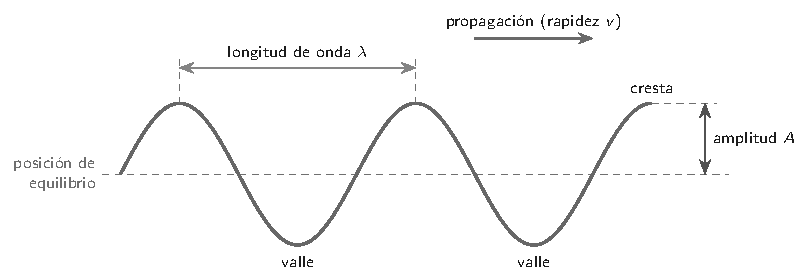
\includegraphics[max width=0.92\linewidth,max height=8.5cm]{fis/ond_elementos}
\end{center}
 
\begin{clave}[{Recuerda}] Prefijos frecuentes: kHz $= 10^3$ Hz, MHz $= 10^6$ Hz, GHz $= 10^9$ Hz; nm $= 10^{-9}$ m, $\mu$m $= 10^{-6}$ m.\end{clave}
\subsection{Rapidez de propagación: v = \ensuremath{\lambda}f}
En un período $T$ la onda avanza exactamente una longitud de onda $\lambda$. Por eso su rapidez de propagación es:

 \[ v = \dfrac{\lambda}{T} = \lambda\, f \] 

De aquí salen las otras dos formas: $\lambda = \dfrac{v}{f}$ y $f = \dfrac{v}{\lambda}$.

 

Todas las ondas electromagnéticas viajan en el vacío con la misma rapidez, la \textbf{rapidez de la luz}:

 \[ c = 3{,}0\times10^{8}\ \text{m/s} = 300\,000\ \text{km/s} \] 

\textbf{Ejemplo.} Una radio FM transmite a $f = 100$ MHz $= 1{,}0\times10^{8}$ Hz. Su longitud de onda es $\lambda = \dfrac{3{,}0\times10^{8}}{1{,}0\times10^{8}} = 3{,}0$ m.

  
\begin{clave}[{Qué depende de qué}] · La \textbf{rapidez} la fija el \textbf{medio}: en un mismo medio, todas las ondas del mismo tipo viajan igual de rápido.\par · La \textbf{frecuencia} la fija la \textbf{fuente} que produce la onda.\par · La \textbf{longitud de onda} se ajusta: $\lambda = v/f$.\end{clave}
 
\begin{clave}[{Recuerda}] En un mismo medio, si la frecuencia se duplica, la longitud de onda se reduce a la mitad: $\lambda$ y $f$ son \textbf{inversamente proporcionales} y su producto, la rapidez, no cambia.\end{clave}
 
\begin{center}\small
\begin{tabular}{@{}ll@{}}
\toprule
\textbf{Onda y medio} & \textbf{Rapidez aproximada} \\
\midrule
Luz en el vacío (y en el aire) & $3{,}0\times10^{8}$ m/s \\
Luz en el agua & $2{,}25\times10^{8}$ m/s \\
Luz en el vidrio & $2{,}0\times10^{8}$ m/s \\
Sonido en el aire & 340 m/s \\
\bottomrule
\end{tabular}
\end{center}
\subsection{Cuando la onda cambia de medio}
Cuando una onda pasa de un medio a otro (por ejemplo, la luz del aire al vidrio):

 
\begin{itemize}
  \item La \textbf{frecuencia no cambia}: la impone la fuente, y cada cresta que llega a la frontera genera una cresta al otro lado.
  \item La \textbf{rapidez cambia}, porque depende del medio.
  \item La \textbf{longitud de onda cambia} en la misma proporción que la rapidez: $\lambda = v/f$.
\end{itemize}
 

\textbf{Ejemplo.} Luz de $f = 6{,}0\times10^{14}$ Hz tiene en el vacío $\lambda = 5{,}0\times10^{-7}$ m. Entra a un material donde su rapidez es la mitad, $1{,}5\times10^{8}$ m/s. Allí la frecuencia sigue siendo $6{,}0\times10^{14}$ Hz y la longitud de onda es

 \[ \lambda = \dfrac{1{,}5\times10^{8}}{6{,}0\times10^{14}} = 2{,}5\times10^{-7}\ \text{m} \] 

La rapidez bajó a la mitad y la longitud de onda también.

  
\begin{clave}[{Recuerda}] El color de la luz está ligado a su frecuencia. Como la frecuencia no cambia al pasar al agua o al vidrio, una luz roja sigue siendo roja dentro del agua.\end{clave}
 
\begin{clave}[{Cómo razonar}] Si te dicen que la onda «entra a otro medio», marca la frecuencia como constante y calcula lo demás con $v = \lambda f$. Si te dicen que la fuente cambia su frecuencia «en el mismo medio», marca la rapidez como constante.\end{clave}
\subsection{La luz viaja en línea recta}
En un medio homogéneo (aire, agua, vidrio) la luz se propaga en \textbf{línea recta}. Para representarla usamos \textbf{rayos}: líneas con una flecha que indica hacia dónde viaja la luz.

 
\begin{itemize}
  \item \textbf{Sombras.} Un objeto opaco bloquea los rayos y detrás queda una zona sin luz con la forma del objeto. Con una fuente pequeña la sombra es nítida; con una fuente grande aparece además una \textbf{penumbra}.
  \item \textbf{Eclipses.} Un eclipse de Sol es la sombra de la Luna sobre la Tierra; uno de Luna, la sombra de la Tierra sobre la Luna.
  \item \textbf{Cámara oscura.} Una caja con un orificio pequeño forma en la cara opuesta una \textbf{imagen invertida} de lo que está afuera: los rayos de la parte alta del objeto cruzan el orificio y llegan abajo, y los de la parte baja llegan arriba.
\end{itemize}
  
\begin{clave}[{Sombras y proporciones}] Con una fuente puntual, la sombra es una ampliación del objeto. Si un objeto de 10 cm está a 1 m de la ampolleta y la pared está a 3 m de la ampolleta, la sombra mide $10 \cdot \dfrac{3}{1} = 30$ cm.\end{clave}
 
\begin{clave}[{Recuerda}] La luz sí puede doblar sus rayos: al cambiar de medio (refracción) o al rebotar (reflexión). Lo que no hace es curvarse dentro de un mismo medio homogéneo.\end{clave}
\subsection{Lo clave del tema}
\begin{center}\small
\begin{tabularx}{\linewidth}{@{}>{\raggedright\arraybackslash\hsize=0.79\hsize}X>{\raggedright\arraybackslash\hsize=1.36\hsize}X>{\raggedright\arraybackslash\hsize=0.34\hsize}X>{\raggedright\arraybackslash\hsize=1.51\hsize}X@{}}
\toprule
\textbf{Concepto} & \textbf{Qué es} & \textbf{Unidad} & \textbf{Qué lo determina} \\
\midrule
Amplitud $A$ & desde el equilibrio hasta una cresta & m & la energía que entrega la fuente \\
Longitud de onda $\lambda$ & distancia entre crestas consecutivas & m & $\lambda = v/f$ \\
Período $T$ & tiempo de un ciclo & s & la fuente; $T = 1/f$ \\
Frecuencia $f$ & ciclos por segundo & Hz & la fuente; no cambia al cambiar de medio \\
Rapidez $v$ & qué tan rápido avanza la onda & m/s & el medio; $v = \lambda f$ \\
\bottomrule
\end{tabularx}
\end{center}
 
\begin{clave}[{Recuerda}] · Mecánicas: necesitan medio (sonido). Electromagnéticas: viajan también en el vacío, a $c = 3{,}0\times10^{8}$ m/s.\par · En un mismo medio, más frecuencia significa menor longitud de onda.\par · Al cambiar de medio cambian $v$ y $\lambda$; la frecuencia se mantiene.\par · La luz viaja en línea recta: sombras, eclipses y cámara oscura.\end{clave}
 
\begin{clave}[{Método PAES}] 1. Anota los datos con sus unidades y pásalos a SI (MHz a Hz, nm a m). 2. Decide qué se mantiene: la rapidez (mismo medio) o la frecuencia (cambio de medio). 3. Usa $v = \lambda f$ despejando lo que te piden. 4. Revisa el orden de magnitud: la luz visible tiene $\lambda$ de cientos de nanómetros y $f$ cercana a $10^{14}$--$10^{15}$ Hz.\end{clave}
\begin{elejemplo}{PAES Invierno 2027, adaptada}
Una emisora de radio emite ondas electromagnéticas de frecuencia $6{,}0\times10^{7}$ Hz, que se propagan en el aire con una rapidez de $3{,}0\times10^{8}$ m/s.

¿Cuál es la longitud de onda de estas ondas en el aire?
\alts{0,2 m}{5,0 m}{$5{,}0\times10^{3}$ m}{$1{,}8\times10^{16}$ m}
\solucion{\textbf{Paso 1. ¿Qué nos piden?} La longitud de onda, conociendo la frecuencia y la rapidez de la onda.

\textbf{Paso 2. Elige la relación.} De $v = \lambda f$ se despeja $\lambda = \dfrac{v}{f}$.

\textbf{Paso 3. Calcula.} $\lambda = \dfrac{3{,}0\times10^{8}}{6{,}0\times10^{7}} = 0{,}5\times10^{1} = 5{,}0$ m.

\textbf{Respuesta:} 5,0 m.

\textbf{¿Por qué no las otras?} 0,2 m sale de invertir la división ($f/v$). $5{,}0\times10^{3}$ m resulta de restar mal los exponentes. $1{,}8\times10^{16}$ m es el producto $v \cdot f$, que no tiene unidades de longitud.

\textbf{\color{cienciaD}Para recordar.} Longitud de onda = rapidez dividida por frecuencia.}{B}
\end{elejemplo}

%% =====================================================================
%% fis_espectro
\section[Espectro electromagnético]{Espectro electromagnético}
\modcomun\ \ {\color{gris}\itshape El orden de las ondas electromagnéticas según su longitud de onda y su frecuencia, los usos tecnológicos de cada rango, la luz visible, la rapidez común en el vacío, y la interferencia y la difracción en términos cualitativos.\par}
\subsection{El espectro electromagnético}
Las ondas electromagnéticas forman una familia continua llamada \textbf{espectro electromagnético}. Todas son la misma clase de onda; lo que cambia es su \textbf{frecuencia} y, por lo tanto, su \textbf{longitud de onda}.

 

Ordenadas de \textbf{menor a mayor frecuencia} (y de mayor a menor longitud de onda):

 
\begin{center}
\textbf{radio \ensuremath{\rightarrow} microondas \ensuremath{\rightarrow} infrarrojo \ensuremath{\rightarrow} luz visible \ensuremath{\rightarrow} ultravioleta \ensuremath{\rightarrow} rayos X \ensuremath{\rightarrow} rayos gamma}
\end{center}
 
\begin{itemize}
  \item Todas viajan en el vacío a la misma rapidez, $c = 3{,}0\times10^{8}$ m/s.
  \item Como $c = \lambda f$, si la frecuencia aumenta, la longitud de onda disminuye.
  \item La \textbf{energía} que transporta la radiación aumenta con la frecuencia. Por eso el ultravioleta, los rayos X y los rayos gamma pueden dañar las células.
\end{itemize}
  
\begin{center}
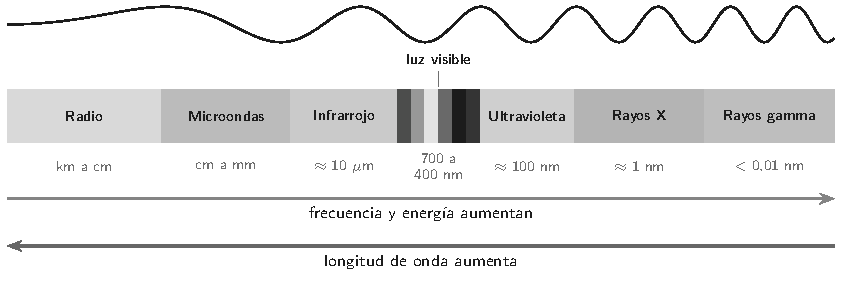
\includegraphics[max width=0.92\linewidth,max height=8.5cm]{fis/ond_espectro}
\end{center}
 
\gatotip[\gatogris]{\textbf{Truco para recordar el orden.} Piensa en el daño: radio y microondas atraviesan tu cuerpo sin dañarlo; el ultravioleta quema la piel; los rayos X y gamma son peligrosos. El daño crece con la frecuencia.}
\subsection{Usos tecnológicos de cada rango}
\begin{center}\small
\begin{tabularx}{\linewidth}{@{}>{\raggedright\arraybackslash\hsize=0.58\hsize}X>{\raggedright\arraybackslash\hsize=0.88\hsize}X>{\raggedright\arraybackslash\hsize=1.54\hsize}X@{}}
\toprule
\textbf{Rango} & \textbf{Longitud de onda típica} & \textbf{Usos y ejemplos} \\
\midrule
Ondas de radio & km a cm & radio AM y FM, televisión abierta, radiotelescopios, comunicación con barcos y aviones \\
Microondas & cm a mm & hornos microondas, wifi, bluetooth, telefonía móvil, radar, comunicación satelital, GPS \\
Infrarrojo & µm & controles remotos, cámaras térmicas y de visión nocturna, calefactores, fibra óptica; todo cuerpo tibio emite infrarrojo \\
Luz visible & 700 a 400 nm & visión, iluminación, fotografía, láser, pantallas \\
Ultravioleta & \textasciitilde{}100 nm & esterilización de agua e instrumentos, detección de billetes falsos, síntesis de vitamina D; produce quemaduras solares \\
Rayos X & \textasciitilde{}1 nm & radiografías, escáneres de equipaje, estudio de cristales \\
Rayos gamma & < 0,01 nm & radioterapia contra el cáncer, esterilización de alimentos y material médico \\
\bottomrule
\end{tabularx}
\end{center}
 
\begin{clave}[{Recuerda}] Los celulares, el wifi y el horno usan microondas, pero de distinta potencia: el horno concentra mucha energía en un espacio cerrado; el teléfono emite muy poca. La radiación de radio y microondas es \textbf{no ionizante}; la de rayos X y gamma es \textbf{ionizante}.\end{clave}
\subsection{La luz visible y los colores}
La \textbf{luz visible} es la pequeña parte del espectro que detectan nuestros ojos, entre unos \textbf{700 nm} (rojo) y \textbf{400 nm} (violeta).

 
\begin{center}\small
\begin{tabular}{@{}ll@{}}
\toprule
\textbf{Color} & \textbf{Longitud de onda aproximada} \\
\midrule
Rojo & 700 a 620 nm \\
Naranjo & 620 a 590 nm \\
Amarillo & 590 a 570 nm \\
Verde & 570 a 495 nm \\
Azul & 495 a 450 nm \\
Violeta & 450 a 400 nm \\
\bottomrule
\end{tabular}
\end{center}
  
\begin{itemize}
  \item El \textbf{rojo} tiene la mayor longitud de onda y la menor frecuencia de la luz visible.
  \item El \textbf{violeta} tiene la menor longitud de onda y la mayor frecuencia.
  \item Más allá del rojo está el \textbf{infrarrojo} («bajo el rojo»); más allá del violeta, el \textbf{ultravioleta}.
  \item La luz blanca del Sol es una mezcla de todos los colores.
\end{itemize}
 
\begin{clave}[{Recuerda}] En el vacío la luz roja y la violeta viajan igual de rápido. Lo que las distingue es su frecuencia (y su longitud de onda), no su rapidez.\end{clave}
\subsection{Interferencia y difracción}
\textbf{Interferencia.} Cuando dos ondas coinciden en un mismo lugar, se superponen. Si llegan cresta con cresta se refuerzan (\textbf{interferencia constructiva}); si llega cresta con valle se anulan (\textbf{interferencia destructiva}).

 

En el \textbf{experimento de la doble rendija de Young}, luz de una sola fuente pasa por dos rendijas muy finas y muy juntas. En la pantalla aparecen \textbf{franjas} claras (interferencia constructiva) y oscuras (destructiva). Para que se vea el patrón, las rendijas deben ser de un tamaño comparable a la longitud de onda y la luz debe ser de una sola frecuencia, como la de un láser.

 

\textbf{Difracción.} Es la capacidad de una onda de \textbf{rodear obstáculos y abrirse al pasar por una abertura}. Se nota cuando la abertura o el obstáculo tiene un tamaño parecido a la longitud de onda.

  
\begin{ejemplo}[{Ejemplos}] · Las ondas de radio AM, con longitudes de onda de cientos de metros, rodean cerros y edificios: se reciben aunque no se vea la antena.\par · La luz, con longitudes de onda de cientos de nanómetros, no rodea una pared, pero sí se difracta en una rendija del grosor de un cabello.\par · Los colores de un CD o de una pompa de jabón se deben a la interferencia de la luz.\end{ejemplo}
 
\begin{clave}[{Recuerda}] La interferencia y la difracción son comportamientos propios de las ondas. El experimento de Young fue una prueba clave de que la luz es una onda.\end{clave}
\subsection{Lo clave del tema}
\begin{center}\small
\begin{tabularx}{\linewidth}{@{}>{\raggedright\arraybackslash\hsize=0.62\hsize}X>{\raggedright\arraybackslash\hsize=1.38\hsize}X@{}}
\toprule
\textbf{Idea} & \textbf{Lo que debes saber} \\
\midrule
Orden del espectro & radio, microondas, infrarrojo, visible, ultravioleta, rayos X, gamma: la frecuencia y la energía aumentan, la longitud de onda disminuye \\
Rapidez & todas viajan a $3{,}0\times10^{8}$ m/s en el vacío \\
Luz visible & entre el infrarrojo y el ultravioleta; rojo (700 nm, menor $f$) a violeta (400 nm, mayor $f$) \\
Interferencia & superposición de ondas: franjas claras y oscuras (Young) \\
Difracción & la onda rodea obstáculos o se abre en aberturas de tamaño comparable a $\lambda$ \\
\bottomrule
\end{tabularx}
\end{center}
 
\begin{clave}[{Método PAES}] 1. Ubica cada radiación en el espectro antes de comparar. 2. Recuerda que la rapidez en el vacío es la misma para todas. 3. En difracción, compara el tamaño de la abertura con la longitud de onda.\end{clave}
\begin{elejemplo}{Estilo PAES}
¿Cuál de las siguientes opciones ordena estas radiaciones de \textbf{menor a mayor frecuencia}: rayos X, ondas de radio, luz visible y microondas?
\begin{center}
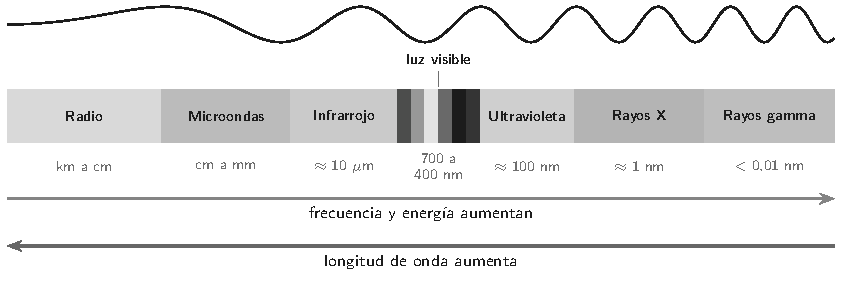
\includegraphics[max width=0.92\linewidth,max height=8.5cm]{fis/ond_espectro}
\end{center}
\altslargas{rayos X, luz visible, microondas, ondas de radio}{ondas de radio, microondas, luz visible, rayos X}{microondas, ondas de radio, rayos X, luz visible}{luz visible, microondas, ondas de radio, rayos X}
\solucion{\textbf{Paso 1. ¿Qué nos piden?} Ordenar cuatro radiaciones según su frecuencia, de menor a mayor.

\textbf{Paso 2. Ubícalas en el espectro.} De izquierda a derecha (frecuencia creciente): radio, microondas, infrarrojo, visible, ultravioleta, rayos X, gamma.

\textbf{Paso 3. Extrae las cuatro.} Ondas de radio, microondas, luz visible, rayos X.

\textbf{Respuesta:} ondas de radio, microondas, luz visible, rayos X.

\textbf{¿Por qué no las otras?} «Rayos X, luz visible, microondas, ondas de radio» es el orden inverso, de mayor a menor frecuencia (que coincide con el orden de menor a mayor longitud de onda). Las otras dos mezclan el orden: las microondas tienen mayor frecuencia que las ondas de radio, y la luz visible menor que los rayos X.

\textbf{\color{cienciaD}Para recordar.} Radio, microondas, infrarrojo, visible, ultravioleta, X, gamma: la frecuencia sube.}{B}
\end{elejemplo}

%% =====================================================================
%% fis_luz
\section[Reflexión, refracción y color]{Reflexión, refracción y color}
\modcomun\ \ {\color{gris}\itshape Qué le ocurre a la luz al llegar a un material (absorción, reflexión y transmisión), la ley de reflexión, la refracción como cambio de rapidez y de dirección y la formación de los colores de los objetos.\par}
\subsection{Qué le pasa a la luz al llegar a un material}
Cuando la luz llega a la superficie de un material, se reparte de tres formas:

 
\begin{itemize}
  \item \textbf{Reflexión:} una parte rebota y vuelve al medio del que venía.
  \item \textbf{Absorción:} una parte es absorbida por el material y su energía lo calienta.
  \item \textbf{Transmisión:} una parte atraviesa el material y sigue al otro lado.
\end{itemize}
 

La energía se conserva: \textbf{incidente = reflejada + absorbida + transmitida}. Si se mide que pasa el 70 \% de la radiación, el material transmite el 70 \%; el 30 \% restante se reflejó o se absorbió.

 

Según cuánto transmiten, los materiales son \textbf{transparentes} (dejan pasar la luz y se ve con nitidez a través de ellos: vidrio, agua), \textbf{translúcidos} (dejan pasar luz, pero no se ve con nitidez: papel mantequilla, vidrio esmerilado) u \textbf{opacos} (no dejan pasar luz: madera, metal).

  
\begin{clave}[{Recuerda}] Un material puede ser transparente a un rango del espectro y opaco a otro. El vidrio deja pasar la luz visible pero absorbe buena parte del ultravioleta; el cuerpo humano es opaco a la luz pero deja pasar los rayos X.\end{clave}
 
\begin{ejemplo}[{Ejemplo PAES}] Se recomienda usar protector solar aunque estés dentro del agua: el agua \textbf{transmite} parte de la radiación ultravioleta, que llega a tu piel.\end{ejemplo}
\subsection{Reflexión de la luz}
Para describir la reflexión se usa la \textbf{normal}: una recta perpendicular a la superficie en el punto donde llega el rayo. Los ángulos se miden \textbf{desde la normal}, no desde la superficie.

 

\textbf{Ley de reflexión:}

 
\begin{itemize}
  \item El ángulo de incidencia es igual al ángulo de reflexión: $\alpha = \beta$.
  \item El rayo incidente, el rayo reflejado y la normal están en un mismo plano.
\end{itemize}
 

\textbf{Reflexión especular y difusa.} En una superficie lisa (espejo, agua quieta) los rayos paralelos se reflejan paralelos y se forma una imagen. En una superficie rugosa (papel, pared) cada rayo se refleja en una dirección distinta: la luz se esparce y no se forma imagen, pero el objeto se ve desde todos lados.

 

En la reflexión no cambian ni la rapidez, ni la frecuencia, ni la longitud de onda: la luz sigue en el mismo medio.

  
\begin{center}
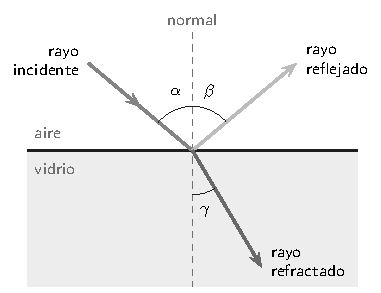
\includegraphics[max width=0.92\linewidth,max height=8.5cm]{fis/ond_reflex_refrac}
\end{center}
 
\begin{clave}[{Recuerda}] Si un rayo forma 30° con la superficie del espejo, forma 60° con la normal: el ángulo de incidencia es 60° y el de reflexión también.\end{clave}
\subsection{Refracción de la luz}
La \textbf{refracción} es el cambio de dirección que experimenta la luz al pasar de un medio a otro con incidencia oblicua. Su causa es el \textbf{cambio de rapidez}.

 

El \textbf{índice de refracción} $n$ indica cuánto se frena la luz en un medio: $n = c/v$. Mientras mayor es $n$, más lenta va la luz.

 
\begin{center}\small
\begin{tabular}{@{}ll@{}}
\toprule
\textbf{Medio} & \textbf{$n$ aproximado} \\
\midrule
Aire & 1,00 \\
Agua & 1,33 \\
Vidrio & 1,5 \\
Diamante & 2,4 \\
\bottomrule
\end{tabular}
\end{center}
 
\begin{itemize}
  \item Si la luz pasa a un medio \textbf{más lento} (mayor $n$), el rayo refractado \textbf{se acerca a la normal}: $\gamma < \alpha$.
  \item Si pasa a un medio \textbf{más rápido} (menor $n$), \textbf{se aleja de la normal}.
  \item Si incide \textbf{perpendicularmente}, no cambia de dirección, aunque sí de rapidez.
\end{itemize}
  
\begin{clave}[{Qué cambia y qué no}] Al refractarse, cambian la \textbf{rapidez}, la \textbf{longitud de onda} y la \textbf{dirección}. La \textbf{frecuencia} (y por lo tanto el color) \textbf{no cambia}.\end{clave}
 
\begin{ejemplo}[{Ejemplos}] · Una cuchara se ve quebrada en un vaso con agua.\par · El fondo de una piscina parece menos profundo de lo que es: la luz que sale del agua se aleja de la normal y el ojo la prolonga en línea recta desde un punto más alto.\end{ejemplo}
 
\begin{clave}[{Reflexión total interna}] Si la luz va de un medio más lento a uno más rápido (del vidrio al aire) con un ángulo mayor que un cierto \textbf{ángulo límite}, no sale: se refleja por completo. Es la base de la fibra óptica.\end{clave}
\subsection{El color de los objetos}
Un objeto se ve del color de la luz que \textbf{refleja} (o transmite) y absorbe el resto:

 
\begin{itemize}
  \item Una manzana roja iluminada con luz blanca refleja el rojo y absorbe los demás colores.
  \item Un objeto \textbf{blanco} refleja todos los colores; uno \textbf{negro} los absorbe casi todos, por eso se calienta más al sol.
  \item Si la luz que llega no contiene el color que el objeto refleja, el objeto se ve \textbf{negro}: una manzana roja iluminada solo con luz azul se ve negra.
  \item Un \textbf{filtro} verde transmite la luz verde y absorbe los demás colores.
\end{itemize}
 

\textbf{Mezcla de luces (aditiva).} Los colores primarios de la luz son rojo, verde y azul. Al superponer luces:

 
\begin{center}\small
\begin{tabular}{@{}ll@{}}
\toprule
\textbf{Luces} & \textbf{Se ve} \\
\midrule
rojo + verde & amarillo \\
rojo + azul & magenta (fucsia) \\
verde + azul & cian \\
rojo + verde + azul & blanco \\
\bottomrule
\end{tabular}
\end{center}
  
\begin{clave}[{Sombras de colores}] Si una luz roja y una verde iluminan una pared blanca, la pared se ve amarilla. Un objeto en medio proyecta dos sombras: donde bloquea la luz roja solo llega verde (sombra verde), y donde bloquea la verde solo llega roja (sombra roja).\end{clave}
 
\begin{clave}[{Recuerda}] Las pantallas de televisores y celulares forman todos los colores encendiendo, en distinta medida, puntos rojos, verdes y azules.\end{clave}
\subsection{Lo clave del tema}
\begin{center}\small
\begin{tabularx}{\linewidth}{@{}>{\raggedright\arraybackslash\hsize=0.49\hsize}X>{\raggedright\arraybackslash\hsize=1.39\hsize}X>{\raggedright\arraybackslash\hsize=1.39\hsize}X>{\raggedright\arraybackslash\hsize=0.73\hsize}X@{}}
\toprule
\textbf{Fenómeno} & \textbf{Qué ocurre} & \textbf{Qué cambia} & \textbf{Ejemplo} \\
\midrule
Absorción & el material retiene la energía & la intensidad que sigue & ropa negra al sol \\
Reflexión & la luz rebota; ángulo de incidencia = ángulo de reflexión & la dirección & espejo \\
Transmisión & la luz atraviesa el material & depende del material & vidrio de una ventana \\
Refracción & cambio de dirección al cambiar de medio & rapidez, $\lambda$ y dirección; no la frecuencia & cuchara quebrada \\
\bottomrule
\end{tabularx}
\end{center}
 
\begin{clave}[{Recuerda}] · Los ángulos se miden desde la normal.\par · Hacia un medio más lento, el rayo se acerca a la normal; hacia uno más rápido, se aleja.\par · El color depende de la frecuencia, que no cambia al refractarse.\par · Un objeto se ve del color que refleja; sin ese color en la luz, se ve negro.\end{clave}
 
\begin{clave}[{Método PAES}] 1. Identifica si la luz rebota (reflexión), cambia de medio (refracción) o es absorbida. 2. Dibuja la normal y mide los ángulos desde ella. 3. Compara las rapideces de los medios para saber hacia dónde se desvía el rayo. 4. En preguntas de investigación, fíjate en qué variable se cambia y cuál se mide.\end{clave}
\begin{elejemplo}{Estilo PAES}
La figura muestra un rayo de luz monocromática que llega desde el aire a la superficie de un vidrio. Parte de la luz se refleja y parte se refracta.

¿Cuál de las siguientes afirmaciones es correcta?
\begin{center}
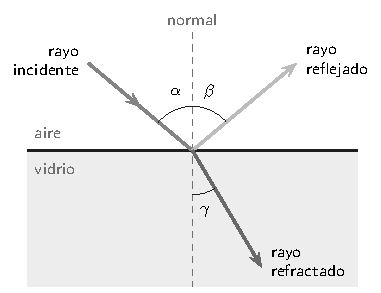
\includegraphics[max width=0.92\linewidth,max height=8.5cm]{fis/ond_reflex_refrac}
\end{center}
\altslargas{En el vidrio, la rapidez y la longitud de onda de la luz disminuyen, y su frecuencia se mantiene.}{El ángulo de reflexión $\beta$ es mayor que el ángulo de incidencia $\alpha$.}{El ángulo $\gamma$ es menor que $\alpha$ porque la frecuencia de la luz disminuye en el vidrio.}{El rayo reflejado tiene menor frecuencia que el rayo incidente.}
\solucion{\textbf{Paso 1. ¿Qué nos piden?} Una afirmación correcta sobre la reflexión y la refracción en la figura.

\textbf{Paso 2. Refracción.} El rayo refractado se acerca a la normal ($\gamma < \alpha$): la luz pasó a un medio donde va más lenta. Con la frecuencia constante, $\lambda = v/f$ también disminuye.

\textbf{Respuesta:} en el vidrio disminuyen la rapidez y la longitud de onda, y la frecuencia se mantiene.

\textbf{¿Por qué no las otras?} Por la ley de reflexión, $\beta = \alpha$. La frecuencia no cambia al refractarse: el rayo se acerca a la normal porque disminuye la rapidez. La reflexión tampoco cambia la frecuencia.

\textbf{\color{cienciaD}Para recordar.} Hacia el vidrio: menor rapidez y menor \ensuremath{\lambda}, misma frecuencia.}{A}
\end{elejemplo}

%% =====================================================================
%% fis_espejos_lentes
\section[Espejos y lentes]{Espejos y lentes}
\modcomun\ \ {\color{gris}\itshape Formación de imágenes en espejos planos, cóncavos y convexos y en lentes convergentes y divergentes: elementos (vértice, foco, centro de curvatura), rayos principales e imágenes reales o virtuales, derechas o invertidas, mayores o menores.\par}
\subsection{Imágenes y espejos planos}
Una \textbf{imagen} es el punto (o conjunto de puntos) desde donde parecen venir los rayos de luz después de reflejarse o refractarse.

 
\begin{itemize}
  \item \textbf{Imagen real:} los rayos realmente se cruzan en ella. Se puede \textbf{proyectar en una pantalla}.
  \item \textbf{Imagen virtual:} solo se cruzan las prolongaciones de los rayos. Se ve mirando el espejo o la lente, pero \textbf{no se puede proyectar}.
\end{itemize}
 

\textbf{Espejo plano.} La imagen es siempre:

 
\begin{itemize}
  \item \textbf{virtual} (está «detrás» del espejo);
  \item \textbf{derecha} (no se invierte de arriba a abajo);
  \item del \textbf{mismo tamaño} que el objeto;
  \item a la \textbf{misma distancia} del espejo que el objeto, pero detrás de él.
\end{itemize}
  
\begin{clave}[{Izquierda y derecha}] Si levantas tu mano derecha frente a un espejo, tu imagen levanta la mano que está a tu derecha, que para ella sería la izquierda. Por eso la palabra AMBULANCIA se escribe al revés en el capó: en el retrovisor del auto de adelante se lee bien.\end{clave}
 
\begin{clave}[{Recuerda}] Si estás a 2 m de un espejo plano, tu imagen está 2 m detrás del espejo: la distancia entre tú y tu imagen es 4 m.\end{clave}
\subsection{Espejos curvos: elementos y rayos principales}
Un \textbf{espejo cóncavo} refleja por su cara interior, como el interior de una cuchara; concentra la luz (es convergente). Un \textbf{espejo convexo} refleja por su cara exterior, como el dorso de una cuchara; dispersa la luz (es divergente).

 
\begin{itemize}
  \item \textbf{Vértice (V):} centro del espejo.
  \item \textbf{Eje óptico:} recta que pasa por el vértice y el centro de curvatura.
  \item \textbf{Centro de curvatura (C):} centro de la esfera de la que forma parte el espejo.
  \item \textbf{Foco (F):} punto medio entre C y V; en él se concentran los rayos que llegan paralelos al eje.
\end{itemize}
  

\textbf{Rayos principales en un espejo cóncavo} (basta dibujar dos para ubicar la imagen):

 
\begin{enumerate}
  \item Un rayo \textbf{paralelo al eje} se refleja pasando por el \textbf{foco}.
  \item Un rayo que pasa por el \textbf{foco} se refleja \textbf{paralelo al eje}.
  \item Un rayo que pasa por el \textbf{centro de curvatura} se refleja sobre sí mismo.
\end{enumerate}
 

En un espejo convexo, F y C están detrás del espejo: un rayo paralelo se refleja como si viniera del foco, y un rayo que apunta al foco se refleja paralelo.

 
\begin{clave}[{Recuerda}] Si pones una fuente de luz en el foco de un espejo cóncavo, los rayos salen paralelos: así funcionan los focos de los autos, las linternas y los faros.\end{clave}
\subsection{Imágenes en espejos cóncavos}
La imagen depende de dónde esté el objeto:

 
\begin{center}\small
\begin{tabular}{@{}ll@{}}
\toprule
\textbf{Posición del objeto} & \textbf{Imagen} \\
\midrule
más allá de C & real, invertida, menor \\
en C & real, invertida, de igual tamaño \\
entre C y F & real, invertida, mayor \\
en F & no se forma (los rayos salen paralelos) \\
entre F y V & virtual, derecha, mayor \\
\bottomrule
\end{tabular}
\end{center}
 

\textbf{Usos:} espejos de maquillaje y de dentista (la cara entre F y V: imagen derecha y aumentada), telescopios reflectores, focos y faros.

  
\begin{center}
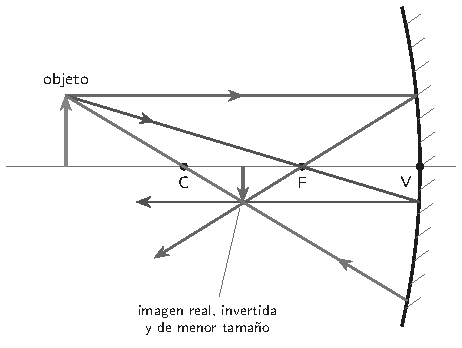
\includegraphics[max width=0.92\linewidth,max height=8.5cm]{fis/ond_espejo_concavo}
\end{center}
 
\begin{clave}[{Recuerda}] En un espejo cóncavo las imágenes reales son siempre invertidas; la única imagen derecha es la virtual, cuando el objeto está entre F y V.\end{clave}
\subsection{Espejos convexos}
En un espejo convexo, sin importar dónde esté el objeto, la imagen es siempre:

 
\begin{itemize}
  \item \textbf{virtual} (detrás del espejo, entre V y F),
  \item \textbf{derecha},
  \item de \textbf{menor tamaño} que el objeto.
\end{itemize}
 

Como las imágenes son más pequeñas, en el espejo cabe una zona mucho más amplia: tiene un gran \textbf{campo visual}.

 

\textbf{Usos:} espejos laterales de los autos, espejos de seguridad en tiendas, estacionamientos y curvas peligrosas.

 
\begin{clave}[{«Los objetos pueden estar más cerca de lo que aparentan»}] Esta advertencia aparece en los espejos laterales porque son convexos: la imagen es más pequeña que el objeto, y el cerebro interpreta que el objeto está más lejos.\end{clave}
  
\begin{center}
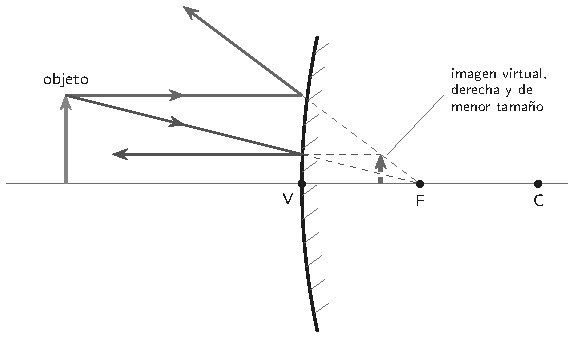
\includegraphics[max width=0.92\linewidth,max height=8.5cm]{fis/ond_espejo_convexo}
\end{center}
\subsection{Lentes convergentes}
Una lente \textbf{convergente} es más gruesa en el centro que en los bordes. Los rayos que llegan paralelos al eje se refractan y se juntan en el \textbf{foco} del otro lado. Tiene un foco a cada lado, a la misma distancia.

 

\textbf{Rayos principales:} (1) un rayo paralelo al eje sale pasando por el foco del otro lado; (2) un rayo que pasa por el centro de la lente no se desvía; (3) un rayo que pasa por el foco del lado del objeto sale paralelo al eje.

 
\begin{center}\small
\begin{tabularx}{\linewidth}{@{}>{\raggedright\arraybackslash\hsize=0.88\hsize}X>{\raggedright\arraybackslash\hsize=1.06\hsize}X>{\raggedright\arraybackslash\hsize=1.06\hsize}X@{}}
\toprule
\textbf{Posición del objeto} & \textbf{Imagen} & \textbf{Uso} \\
\midrule
más allá de 2F & real, invertida, menor & cámara fotográfica, ojo \\
en 2F & real, invertida, igual & fotocopiadora \\
entre 2F y F & real, invertida, mayor & proyector \\
en F & no se forma & linterna, faro \\
entre F y la lente & virtual, derecha, mayor & lupa \\
\bottomrule
\end{tabularx}
\end{center}
  
\begin{center}
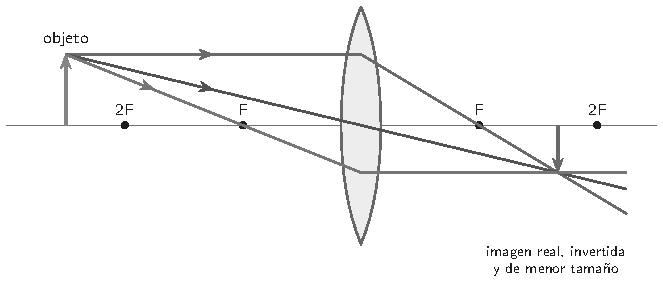
\includegraphics[max width=0.92\linewidth,max height=8.5cm]{fis/ond_lente_conv}
\end{center}
 
\begin{clave}[{Recuerda}] Las lentes convergentes se usan para corregir la \textbf{hipermetropía}.\end{clave}
\subsection{Lentes divergentes}
Una lente \textbf{divergente} es más delgada en el centro que en los bordes. Los rayos que llegan paralelos al eje se separan al atravesarla, como si vinieran del foco ubicado del lado del objeto.

 

Sin importar la posición del objeto, la imagen es siempre \textbf{virtual, derecha y de menor tamaño}, y está del mismo lado que el objeto, entre el foco y la lente.

 

\textbf{Usos:} mirillas de las puertas (dan una vista amplia), lentes para corregir la \textbf{miopía}, combinadas con lentes convergentes en cámaras y telescopios.

 
\begin{clave}[{Paralelo con los espejos}] · Espejo cóncavo y lente convergente: imágenes reales o virtuales según la posición.\par · Espejo convexo y lente divergente: siempre virtual, derecha y menor.\end{clave}
  
\begin{center}
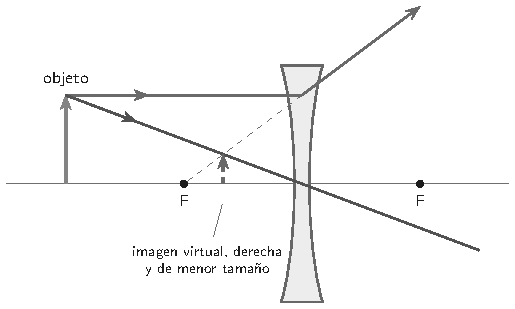
\includegraphics[max width=0.92\linewidth,max height=8.5cm]{fis/ond_lente_div}
\end{center}
\subsection{Lo clave del tema}
\begin{center}\small
\begin{tabularx}{\linewidth}{@{}>{\raggedright\arraybackslash\hsize=0.54\hsize}X>{\raggedright\arraybackslash\hsize=1.26\hsize}X>{\raggedright\arraybackslash\hsize=1.20\hsize}X@{}}
\toprule
\textbf{Elemento} & \textbf{Tipo de imagen} & \textbf{Usos típicos} \\
\midrule
Espejo plano & virtual, derecha, igual tamaño, a la misma distancia & espejos de baño, retrovisor interior \\
Espejo cóncavo & real e invertida (objeto más allá de F) o virtual, derecha y mayor (objeto entre F y V) & maquillaje, faros, telescopios \\
Espejo convexo & siempre virtual, derecha y menor & espejos laterales, seguridad \\
Lente convergente & real e invertida (objeto más allá de F) o virtual, derecha y mayor (objeto entre F y la lente) & lupa, proyector, cámara, hipermetropía \\
Lente divergente & siempre virtual, derecha y menor & mirillas, miopía \\
\bottomrule
\end{tabularx}
\end{center}
 
\begin{clave}[{Recuerda}] · Real = se proyecta en pantalla = invertida. Virtual = no se proyecta = derecha.\par · Con el objeto en el foco no se forma imagen: los rayos salen paralelos.\par · Paralelo al eje \ensuremath{\rightarrow} por el foco; por el foco \ensuremath{\rightarrow} paralelo al eje.\end{clave}
 
\begin{clave}[{Método PAES}] 1. Identifica el elemento (plano, cóncavo, convexo, convergente, divergente). 2. Si es convexo o divergente, la imagen es virtual, derecha y menor. 3. Si es cóncavo o convergente, ubica el objeto respecto de F y de C (o 2F) y usa la tabla. 4. En diagramas, verifica cada rayo con las reglas de los rayos principales.\end{clave}
\begin{elejemplo}{PAES Invierno 2027, adaptada}
Un joven viaja de copiloto en un furgón escolar y nota que el espejo lateral tiene escrita la advertencia «los objetos pueden estar más cerca de lo que aparentan». Le pregunta a la conductora, quien le explica correctamente usando lo que recuerda de física.

¿Cuál pudo ser la respuesta de la conductora?
\altslargas{Que al ser un espejo cóncavo, la imagen formada es invertida y de menor tamaño que los objetos.}{Que al ser un espejo cóncavo, la imagen formada es derecha y de mayor tamaño que los objetos.}{Que al ser un espejo convexo, la imagen formada es derecha y de menor tamaño que los objetos.}{Que al ser un espejo convexo, la imagen formada es invertida y de mayor tamaño que los objetos.}
\solucion{\textbf{Paso 1. ¿Qué nos piden?} Qué tipo de espejo produce la ilusión de que los objetos están más lejos.

\textbf{Paso 2. Piensa en el tamaño.} Si un objeto se ve más pequeño de lo normal, el cerebro interpreta que está más lejos. El espejo lateral debe formar imágenes más pequeñas que los objetos.

\textbf{Paso 3. Elige el espejo.} El espejo convexo forma siempre imágenes virtuales, derechas y menores, y además tiene un campo visual amplio.

\textbf{Respuesta:} es un espejo convexo y la imagen es derecha y de menor tamaño.

\textbf{¿Por qué no las otras?} Una imagen invertida haría ver los autos de cabeza, y un espejo lateral no hace eso. Una imagen mayor haría ver los objetos más cerca, no más lejos. Un espejo convexo nunca forma imágenes invertidas ni mayores.

\textbf{\color{cienciaD}Para recordar.} Espejo convexo: imagen virtual, derecha y menor; los objetos parecen más lejos.}{C}
\end{elejemplo}

%% =====================================================================
%% fis_dispositivos
\section[Dispositivos tecnológicos con ondas]{Dispositivos tecnológicos con ondas}
\modcomun\ \ {\color{gris}\itshape Cómo funcionan y para qué sirven la radio, la televisión, el teléfono móvil y la comunicación inalámbrica, el radar, los radiotelescopios, los telescopios reflector y refractor, los prismáticos, la fibra óptica y el láser.\par}
\subsection{Comunicación inalámbrica}
La radio, la televisión abierta, el teléfono móvil, el wifi, el bluetooth y el GPS transmiten información con \textbf{ondas de radio y microondas}. Todos siguen el mismo esquema:

 
\begin{enumerate}
  \item Un \textbf{emisor} convierte la información (sonido, imagen, datos) en una señal eléctrica.
  \item Una \textbf{antena emisora} la transforma en ondas electromagnéticas de una frecuencia determinada.
  \item Las ondas viajan a $3{,}0\times10^{8}$ m/s y llegan a una \textbf{antena receptora}.
  \item El \textbf{receptor} sintoniza esa frecuencia y recupera la información.
\end{enumerate}
 

La información se «monta» sobre la onda variando su amplitud (\textbf{AM}, amplitud modulada) o su frecuencia (\textbf{FM}, frecuencia modulada). Cada emisora tiene su propia frecuencia, para que las señales no se mezclen.

  
\begin{clave}[{Teléfono móvil}] El celular se comunica por microondas con la antena más cercana. El territorio se divide en zonas llamadas \textbf{celdas}, cada una con su antena; al moverte, la llamada pasa de una antena a otra. Las antenas se conectan entre sí por cables, fibra óptica o enlaces de microondas.\end{clave}
 
\begin{clave}[{Satélites}] Los satélites de comunicaciones reciben microondas desde la Tierra y las reenvían a otro punto. Permiten la televisión satelital, el GPS y las llamadas a lugares remotos.\end{clave}
\subsection{Radar y radiotelescopios}
\textbf{Radar.} Emite pulsos de microondas que se \textbf{propagan}, se \textbf{reflejan} en un objeto (avión, barco, nube de lluvia) y vuelven a la antena.

 

El \textbf{tiempo} de ida y vuelta da la distancia: la onda recorre dos veces la distancia, así que $d = \dfrac{c\,t}{2}$.

 

\textbf{Ejemplo.} Si un pulso vuelve $2{,}0\times10^{-4}$ s después de emitido: $d = \dfrac{3{,}0\times10^{8}\cdot 2{,}0\times10^{-4}}{2} = 3{,}0\times10^{4}$ m $= 30$ km.

 

Se usa en aeronáutica, navegación y meteorología.

  

\textbf{Radiotelescopios.} Grandes antenas parabólicas que captan las \textbf{ondas de radio} que emiten estrellas, galaxias y nubes de gas. La superficie parabólica refleja las ondas y las concentra en su \textbf{foco}, donde está el receptor. Pueden funcionar de día y a través de nubes.

 
\begin{clave}[{Chile y la astronomía}] El observatorio ALMA, en el llano de Chajnantor (Atacama), a unos 5000 m de altura, combina 66 antenas que captan ondas milimétricas. Se instaló allí porque el aire es muy seco: el vapor de agua absorbe esas ondas.\end{clave}
\subsection{Telescopios y prismáticos}
\textbf{Telescopio refractor.} Usa \textbf{lentes}. Una lente convergente grande (el \textbf{objetivo}) forma una imagen real del objeto lejano, y una segunda lente (el \textbf{ocular}) la amplía como una lupa. Así funcionaba el telescopio de Galileo.

 

\textbf{Telescopio reflector.} Usa un \textbf{espejo cóncavo} (el espejo primario) para reunir la luz y formar la imagen; un espejo secundario la dirige al ocular o a la cámara. Lo diseñó Newton.

 

Los grandes telescopios actuales, como los de Paranal o el ELT en el norte de Chile, son \textbf{reflectores}: un espejo se puede fabricar mucho más grande que una lente y sostenerse por detrás, sin deformarse.

  

\textbf{Prismáticos (binoculares).} Son dos pequeños telescopios refractores, uno para cada ojo. Entre el objetivo y el ocular tienen \textbf{prismas} que reflejan la luz varias veces por \textbf{reflexión total interna}. Los prismas cumplen dos funciones:

 
\begin{itemize}
  \item \textbf{enderezan} la imagen, que el objetivo forma invertida;
  \item \textbf{acortan} el instrumento, porque la luz recorre el camino en zigzag.
\end{itemize}
 
\begin{clave}[{Recuerda}] Mientras mayor es el objetivo (lente o espejo), más luz reúne el telescopio y más débiles son los objetos que puede observar.\end{clave}
\subsection{Fibra óptica}
Una \textbf{fibra óptica} es un hilo muy delgado de vidrio o plástico formado por un \textbf{núcleo}, con mayor índice de refracción, rodeado por un \textbf{revestimiento}, con menor índice.

 

La luz entra por un extremo y, cada vez que llega al límite entre el núcleo y el revestimiento con un ángulo mayor que el ángulo límite, se refleja por completo: \textbf{reflexión total interna}. Así avanza en zigzag por la fibra, aunque esta se curve, y casi sin perder intensidad.

 

\textbf{Usos:} internet y telefonía de alta velocidad (la información viaja como pulsos de luz, normalmente infrarroja), endoscopios médicos que permiten ver el interior del cuerpo, iluminación decorativa.

  
\begin{center}
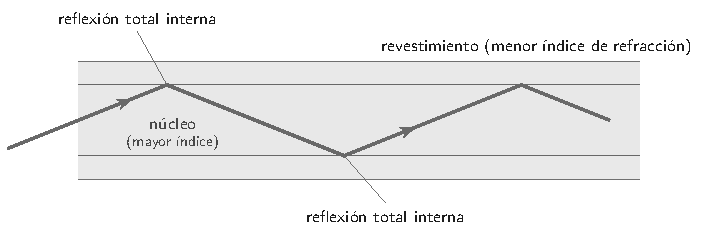
\includegraphics[max width=0.92\linewidth,max height=8.5cm]{fis/ond_fibra}
\end{center}
 
\begin{clave}[{Recuerda}] La reflexión total interna solo ocurre cuando la luz va de un medio donde es más lenta (mayor índice) a uno donde es más rápida (menor índice). Por eso el núcleo debe tener mayor índice que el revestimiento.\end{clave}
\subsection{Láser, pantallas y controles remotos}
\textbf{Láser.} Produce una luz con tres propiedades especiales:

 
\begin{itemize}
  \item \textbf{monocromática:} de una sola frecuencia (un solo color);
  \item \textbf{coherente:} todas sus ondas oscilan en fase;
  \item \textbf{direccional:} el haz casi no se abre, y concentra mucha energía en un punto pequeño.
\end{itemize}
 

\textbf{Usos:} lectores de códigos de barras, medición de distancias, cirugías y tratamientos oculares, corte de materiales, punteros, comunicación por fibra óptica, experimentos de interferencia.

  

\textbf{Televisor y pantallas.} La pantalla está formada por millones de \textbf{píxeles}, cada uno con puntos rojo, verde y azul. Encendiéndolos con distinta intensidad se obtiene cualquier color por \textbf{mezcla aditiva}: rojo y verde dan amarillo; los tres juntos, blanco.

 

\textbf{Control remoto.} Envía pulsos de \textbf{luz infrarroja} que el televisor detecta. Como el infrarrojo no atraviesa objetos opacos, hay que apuntar al televisor sin obstáculos. El wifi, en cambio, usa microondas, que atraviesan en buena medida paredes y muebles.

 
\begin{clave}[{Recuerda}] La cámara de un celular puede ver el destello infrarrojo de un control remoto, aunque tus ojos no lo vean.\end{clave}
\subsection{Lo clave del tema}
\begin{center}\small
\begin{tabularx}{\linewidth}{@{}>{\raggedright\arraybackslash\hsize=1.04\hsize}X>{\raggedright\arraybackslash\hsize=0.73\hsize}X>{\raggedright\arraybackslash\hsize=1.22\hsize}X@{}}
\toprule
\textbf{Dispositivo} & \textbf{Onda que usa} & \textbf{Fenómeno o principio} \\
\midrule
Radio, TV, celular, wifi & radio y microondas & emisión y recepción por antenas; cada señal con su frecuencia \\
Radar & microondas & propagación y reflexión; $d = ct/2$ \\
Radiotelescopio, antena parabólica & radio y microondas & reflexión en una superficie parabólica que concentra en el foco \\
Telescopio refractor & luz visible & refracción en lentes convergentes \\
Telescopio reflector & luz visible e infrarroja & reflexión en un espejo cóncavo \\
Prismáticos & luz visible & lentes y prismas con reflexión total interna \\
Fibra óptica & luz visible e infrarroja & reflexión total interna \\
Láser & luz de una frecuencia & haz monocromático, coherente y direccional \\
Control remoto, cámara térmica & infrarrojo & emisión y detección de infrarrojo \\
\bottomrule
\end{tabularx}
\end{center}
 
\begin{clave}[{Método PAES}] 1. Identifica qué onda usa el dispositivo y ubícala en el espectro. 2. Pregúntate qué le pasa a la onda: se propaga, se refleja, se refracta o se absorbe. 3. En cálculos de radar o comunicación, usa $d = v\,t$ y recuerda si el viaje es de ida o de ida y vuelta.\end{clave}
\begin{elejemplo}{PAES Invierno 2026, adaptada}
El radar se usa ampliamente en aeronáutica, navegación y meteorología, porque permite determinar la posición de objetos y seguir sus trayectorias.

¿Qué fenómenos asociados a las ondas electromagnéticas explican el funcionamiento del radar?
\alts{La difracción y la absorción.}{La refracción y la absorción.}{La propagación y la difracción.}{La propagación y la reflexión.}
\solucion{\textbf{Paso 1. ¿Qué nos piden?} Los fenómenos en que se basa el radar.

\textbf{Paso 2. Sigue la onda.} El radar emite microondas que viajan por el aire hasta el objeto (\textbf{propagación}), rebotan en él (\textbf{reflexión}) y vuelven a la antena. Midiendo el tiempo de ida y vuelta calcula la distancia.

\textbf{Respuesta:} la propagación y la reflexión.

\textbf{¿Por qué no las otras?} Si el objeto absorbiera las microondas, no volvería señal al radar. La refracción y la difracción pueden ocurrir, pero no son la base del funcionamiento: lo esencial es que la onda vaya y vuelva reflejada.

\textbf{\color{cienciaD}Para recordar.} Radar: la onda viaja, se refleja en el objeto y vuelve.}{D}
\end{elejemplo}

\chapter{Mecánica}
%% =====================================================================
%% fis_cinematica
\section[Describir el movimiento]{Describir el movimiento}
\modcomun\ \ {\color{gris}\itshape Sistema de referencia, trayectoria y posición; distancia recorrida frente a desplazamiento; rapidez media frente a velocidad media; velocidad instantánea y aceleración; y relatividad de Galileo con suma de velocidades (trenes, ríos y escaleras mecánicas).\par}
\subsection{Sistema de referencia, posición y trayectoria}
Para describir un movimiento primero se elige un \textbf{sistema de referencia}: un punto de origen, un eje con un sentido positivo y un reloj para medir el tiempo.

 

La \textbf{posición} ($x$) indica dónde está el cuerpo respecto del origen. En una línea recta basta un número con signo: $x = +3$ m está 3 m hacia el lado positivo del origen y $x = -2$ m está 2 m hacia el lado negativo.

 

La \textbf{trayectoria} es la línea que describe el cuerpo al moverse: recta, curva, circular.

 

El \textbf{tiempo transcurrido} entre dos instantes es $\Delta t = t_f - t_i$.

  
\begin{clave}[{El movimiento es relativo}] Un pasajero sentado en un bus está en reposo respecto del bus y en movimiento respecto de la calle. Antes de decir «se mueve» o «está quieto», pregúntate: ¿respecto de qué?\end{clave}
 
\begin{clave}[{Recuerda}] La posición depende del origen que se elija. En cambio, el cambio de posición entre dos instantes es el mismo para dos observadores quietos uno respecto del otro, aunque usen orígenes distintos.\end{clave}
\subsection{Distancia recorrida y desplazamiento}
El \textbf{desplazamiento} es el cambio de posición: \[ \Delta x = x_f - x_i \] Tiene magnitud, dirección y sentido (es un vector). En una recta, su signo indica el sentido.

 

La \textbf{distancia recorrida} ($d$) es el largo total del camino seguido. Siempre es positiva y nunca disminuye mientras el cuerpo se mueve.

 

En la figura, un carrito parte en $x = 2$ m, avanza hasta $x = 10$ m y regresa hasta $x = 6$ m:

 
\begin{itemize}
  \item distancia recorrida: $d = 8 + 4 = 12$ m;
  \item desplazamiento: $\Delta x = 6 - 2 = +4$ m.
\end{itemize}
  
\begin{center}
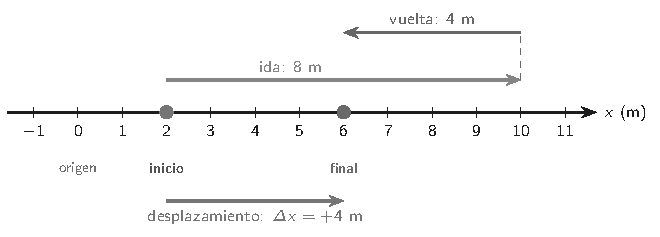
\includegraphics[max width=0.92\linewidth,max height=8.5cm]{fis/mov_trayecto}
\end{center}
 
\begin{clave}[{Recuerda}] La distancia recorrida coincide con la magnitud del desplazamiento solo si el cuerpo se mueve en línea recta sin devolverse. Si vuelve al punto de partida, su desplazamiento es nulo, aunque haya recorrido mucho.\end{clave}
\subsection{Rapidez media y velocidad media}
La \textbf{rapidez media} compara la distancia recorrida con el tiempo empleado:

 
\begin{center}
$\text{rapidez media} = \dfrac{d}{\Delta t}$
\end{center}
 

La \textbf{velocidad media} compara el desplazamiento con el tiempo, y tiene el sentido del desplazamiento:

 
\begin{center}
$v_m = \dfrac{\Delta x}{\Delta t}$
\end{center}
 

\textbf{Ejemplo.} Una persona camina 300 m hacia el este y luego 100 m hacia el oeste, en un total de 200 s. Recorre $d = 400$ m y su desplazamiento es 200 m hacia el este. Su rapidez media es $\dfrac{400}{200} = 2$ m/s y su velocidad media es $\dfrac{200}{200} = 1$ m/s hacia el este.

  
\begin{clave}[{Unidades}] En el SI la rapidez y la velocidad se miden en m/s. Para pasar de km/h a m/s se divide por 3,6: $72$ km/h $= 20$ m/s y $36$ km/h $= 10$ m/s.\end{clave}
 
\begin{clave}[{Recuerda}] La rapidez media no es el promedio de las rapideces. Si recorres 30 km a 60 km/h (0,5 h) y otros 30 km a 30 km/h (1 h), tu rapidez media es $\dfrac{60}{1{,}5} = 40$ km/h, no 45 km/h. Siempre divide la distancia total por el tiempo total, incluidas las detenciones.\end{clave}
\subsection{Velocidad instantánea y aceleración}
La \textbf{velocidad instantánea} es la velocidad en un instante determinado. Su magnitud, la \textbf{rapidez instantánea}, es lo que marca el velocímetro de un auto.

 

La \textbf{aceleración} mide qué tan rápido cambia la velocidad:

 
\begin{center}
$a = \dfrac{\Delta v}{\Delta t} = \dfrac{v_f - v_i}{\Delta t}$
\end{center}
 

Su unidad es m/s². Si un auto pasa de 5 m/s a 25 m/s en 4 s, su aceleración es $a = \dfrac{25 - 5}{4} = 5$ m/s²: cada segundo su velocidad aumenta 5 m/s.

 

En una recta, si la aceleración y la velocidad tienen el \textbf{mismo signo}, la rapidez aumenta; si tienen \textbf{signos opuestos}, la rapidez disminuye (el cuerpo frena).

  
\begin{clave}[{Hay aceleración siempre que cambie la velocidad}] · si aumenta la rapidez;\par · si disminuye la rapidez (frenar también es acelerar);\par · si cambia la dirección, aunque la rapidez sea constante, como un auto que toma una curva con el velocímetro fijo.\end{clave}
 
\begin{clave}[{Recuerda}] Velocidad y aceleración son magnitudes distintas. Una pelota lanzada hacia arriba tiene velocidad nula en el punto más alto y, sin embargo, su aceleración es la de gravedad. Un avión en vuelo recto a velocidad constante tiene gran velocidad y aceleración nula.\end{clave}
\subsection{Relatividad de Galileo}
Galileo observó que dentro de un barco que navega con velocidad constante y sin sacudidas, una pelota cae, rueda y rebota igual que en tierra firme. Ningún experimento mecánico hecho dentro del barco permite saber si se mueve. Las leyes del movimiento son las mismas en todos los sistemas de referencia que se mueven con \textbf{velocidad constante} unos respecto de otros.

 

Lo que sí cambia de un observador a otro son las \textbf{posiciones, las velocidades y las trayectorias}. Para movimientos sobre una misma recta, las velocidades se suman con su signo:

 
\begin{center}
$v_{\text{respecto del suelo}} = v_{\text{respecto del tren}} + v_{\text{tren}}$
\end{center}
 
\begin{itemize}
  \item Tren a 15 m/s y pasajero que camina hacia adelante a 2 m/s: 17 m/s respecto del andén. Si camina hacia atrás: $15 - 2 = 13$ m/s.
  \item Bote a 5 m/s respecto del agua en un río que fluye a 2 m/s: 7 m/s río abajo y 3 m/s río arriba, respecto de la orilla.
\end{itemize}
  
\begin{center}
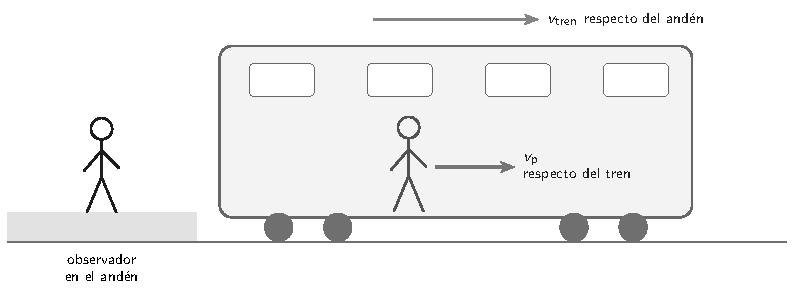
\includegraphics[max width=0.92\linewidth,max height=8.5cm]{fis/mov_tren}
\end{center}
 
\begin{clave}[{Recuerda}] Si un pasajero suelta una moneda en un tren que avanza a velocidad constante, para él la moneda cae en línea recta vertical. Para una persona en el andén, la moneda también avanza junto con el tren y describe una curva. La trayectoria depende del sistema de referencia.\end{clave}
\subsection{Lo clave del tema}
\begin{center}\small
\begin{tabularx}{\linewidth}{@{}>{\raggedright\arraybackslash\hsize=0.76\hsize}X>{\raggedright\arraybackslash\hsize=1.60\hsize}X>{\raggedright\arraybackslash\hsize=1.28\hsize}X>{\raggedright\arraybackslash\hsize=0.36\hsize}X@{}}
\toprule
\textbf{Magnitud} & \textbf{Qué es} & \textbf{Cómo se calcula} & \textbf{Unidad SI} \\
\midrule
Posición & dónde está respecto del origen & $x$ & m \\
Desplazamiento & cambio de posición, con sentido & $\Delta x = x_f - x_i$ & m \\
Distancia recorrida & largo total del camino & suma de los tramos & m \\
Rapidez media & distancia por unidad de tiempo & $d / \Delta t$ & m/s \\
Velocidad media & desplazamiento por unidad de tiempo & $\Delta x / \Delta t$ & m/s \\
Aceleración & cambio de velocidad por unidad de tiempo & $\Delta v / \Delta t$ & m/s² \\
Velocidad relativa & velocidad vista desde otro sistema & en una recta, se suman con signo & m/s \\
\bottomrule
\end{tabularx}
\end{center}
 
\begin{clave}[{Recuerda}] · Si el cuerpo vuelve al punto de partida, su desplazamiento y su velocidad media son nulos.\par · La rapidez media usa el tiempo total, incluidas las detenciones.\par · Frenar y doblar también son formas de acelerar.\par · Posición, velocidad y trayectoria dependen del observador; las leyes del movimiento son las mismas para observadores con velocidad constante entre sí.\end{clave}
 
\begin{clave}[{Método PAES}] 1. Fija el origen y el sentido positivo. 2. Distingue si te piden algo escalar (distancia, rapidez) o vectorial (desplazamiento, velocidad). 3. Usa siempre totales: distancia total y tiempo total. 4. Revisa las unidades (km/h o m/s). 5. En problemas de trenes, ríos o escaleras, pregunta respecto de quién se da cada velocidad antes de sumar.\end{clave}
\begin{elejemplo}{Estilo PAES}
Un carrito de juguete se mueve sobre una pista recta. La figura muestra su recorrido: parte en $x = 2$ m, avanza hasta $x = 10$ m y luego regresa hasta $x = 6$ m. Todo el recorrido dura 4 s.

¿Cuáles son, respectivamente, la rapidez media del carrito y la magnitud de su velocidad media en esos 4 s?
\begin{center}
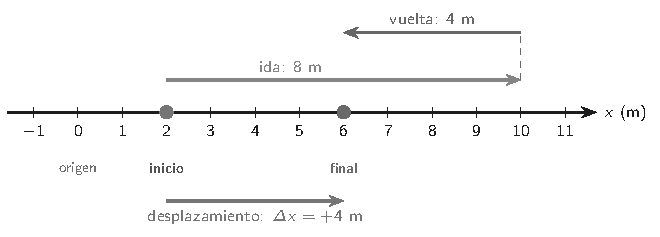
\includegraphics[max width=0.92\linewidth,max height=8.5cm]{fis/mov_trayecto}
\end{center}
\alts{1 m/s y 3 m/s}{3 m/s y 3 m/s}{3 m/s y 1 m/s}{1,5 m/s y 1 m/s}
\solucion{\textbf{Paso 1. ¿Qué nos piden?} Dos magnitudes distintas: la rapidez media, que usa la distancia recorrida, y la velocidad media, que usa el desplazamiento.

\textbf{Paso 2. Distancia recorrida.} Ida de 2 m a 10 m: 8 m. Vuelta de 10 m a 6 m: 4 m. Total: $d = 12$ m.

\textbf{Paso 3. Desplazamiento.} Solo importan la posición final y la inicial: $\Delta x = 6 - 2 = +4$ m.

\textbf{Paso 4. Divide por el tiempo total.} Rapidez media $= \dfrac{12}{4} = 3$ m/s. Velocidad media $= \dfrac{4}{4} = 1$ m/s.

\textbf{Respuesta:} 3 m/s y 1 m/s.

\textbf{¿Por qué no las otras?} «1 m/s y 3 m/s» intercambia las dos magnitudes. «3 m/s y 3 m/s» usa la distancia recorrida también para la velocidad media. «1,5 m/s y 1 m/s» divide la posición final (6 m) por el tiempo, en lugar de la distancia recorrida.

\textbf{\color{cienciaD}Para recordar.} Rapidez media: distancia total / tiempo. Velocidad media: desplazamiento / tiempo.}{C}
\end{elejemplo}

%% =====================================================================
%% fis_mru
\section[Movimiento rectilíneo uniforme]{Movimiento rectilíneo uniforme}
\modcomun\ \ {\color{gris}\itshape Movimiento en línea recta con velocidad constante: ecuación de itinerario x(t) = x0 + v t, lectura de gráficos posición--tiempo (pendiente) y velocidad--tiempo (área), y problemas de encuentro y alcance entre dos móviles.\par}
\subsection{El movimiento rectilíneo uniforme}
Un cuerpo tiene \textbf{movimiento rectilíneo uniforme (MRU)} cuando se mueve en línea recta con \textbf{velocidad constante}: misma rapidez y mismo sentido todo el tiempo. Recorre \textbf{distancias iguales en tiempos iguales} y su aceleración es nula.

 

La \textbf{ecuación de itinerario} entrega la posición en cada instante:

 
\begin{center}
$x(t) = x_0 + v\,t$
\end{center}
 

$x_0$ es la posición inicial (en $t = 0$) y $v$ es la velocidad, con signo: positiva si el cuerpo avanza en el sentido del eje, negativa si avanza en sentido contrario.

 
\begin{itemize}
  \item $x(t) = 5 + 3t$: parte en 5 m y avanza 3 m cada segundo. A los 4 s está en $5 + 12 = 17$ m.
  \item $x(t) = 20 - 4t$: parte en 20 m y se mueve en sentido negativo a 4 m/s. Pasa por el origen cuando $20 - 4t = 0$, es decir, a los 5 s.
\end{itemize}
  
\begin{clave}[{Recuerda}] De la ecuación se obtienen las relaciones de siempre: $\Delta x = v\,t$, $\;t = \dfrac{\Delta x}{v}$, $\;v = \dfrac{\Delta x}{t}$. Usa unidades coherentes: metros con segundos, o kilómetros con horas.\end{clave}
 
\begin{ejemplo}[{Ejemplos de MRU}] La luz viaja en el vacío a $3{,}0\times10^8$ m/s y el sonido en el aire a unos 340 m/s. Por eso, en una tormenta, primero se ve el relámpago y después se oye el trueno.\end{ejemplo}
\subsection{Gráfico posición--tiempo}
En un MRU, el gráfico $x$--$t$ es una \textbf{recta}:

 
\begin{itemize}
  \item donde la recta corta el eje vertical se lee la posición inicial $x_0$;
  \item la \textbf{pendiente} es la velocidad: $v = \dfrac{\Delta x}{\Delta t}$;
  \item recta que sube: velocidad positiva; recta que baja: velocidad negativa; recta horizontal: reposo;
  \item mientras más inclinada, mayor es la rapidez.
\end{itemize}
 

En la figura: A parte del origen con $v_A = \dfrac{32 - 0}{8} = 4$ m/s. B parte en 24 m con $v_B = \dfrac{0 - 24}{8} = -3$ m/s. C está en reposo en $x = 12$ m.

  
\begin{center}
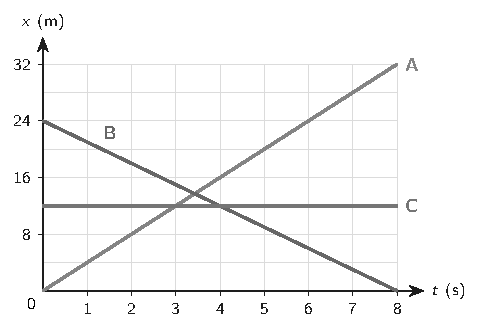
\includegraphics[max width=0.92\linewidth,max height=8.5cm]{fis/mov_mru_xt}
\end{center}
 
\begin{clave}[{Recuerda}] El gráfico $x$--$t$ no es un dibujo de la trayectoria. Una recta que baja no significa que el cuerpo baje por una pendiente: significa que se mueve en el sentido negativo del eje.\end{clave}
\subsection{Gráfico velocidad--tiempo}
En un MRU la velocidad no cambia: el gráfico $v$--$t$ es una \textbf{recta horizontal} a la altura de la velocidad.

 

El \textbf{área} entre esa recta y el eje del tiempo es el \textbf{desplazamiento}: $\Delta x = v\,\Delta t$. En la figura, $v = 5$ m/s durante 6 s: área $= 5\cdot 6 = 30$ m.

 

Si la velocidad es negativa, la recta queda bajo el eje y su área cuenta como desplazamiento negativo. La distancia recorrida suma todas las áreas como positivas.

 

El gráfico aceleración--tiempo de un MRU coincide con el eje del tiempo: $a = 0$.

  
\begin{center}
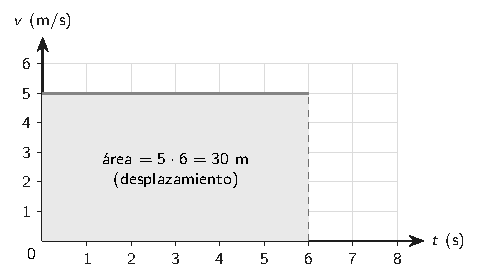
\includegraphics[max width=0.92\linewidth,max height=8.5cm]{fis/mov_mru_vt}
\end{center}
 
\begin{clave}[{Recuerda}] En el gráfico $x$--$t$ se mira la pendiente. En el gráfico $v$--$t$ se mira la altura (la velocidad) y el área (el desplazamiento). Antes de responder, lee qué magnitud hay en cada eje.\end{clave}
\subsection{Encuentros y alcances}
Dos móviles que van por la misma recta se \textbf{encuentran} en el instante en que tienen la \textbf{misma posición}. Método:

 
\begin{enumerate}
  \item Elige un único origen y un único sentido positivo para ambos.
  \item Escribe la ecuación de itinerario de cada uno.
  \item Iguala $x_A(t) = x_B(t)$ y despeja $t$.
  \item Reemplaza ese $t$ en cualquiera de las ecuaciones para saber dónde se encuentran.
\end{enumerate}
 

\textbf{Atajo.} Si se mueven uno hacia el otro, la distancia $D$ que los separa disminuye con la suma de sus rapideces: $t = \dfrac{D}{v_A + v_B}$. Si uno persigue al otro, disminuye con la diferencia: $t = \dfrac{D}{v_A - v_B}$.

  
\begin{ejemplo}[{Ejemplo resuelto}] Un auto A pasa por $x = 0$ a 15 m/s persiguiendo a un camión B, que está en $x = 100$ m y avanza a 10 m/s en el mismo sentido.\par \textbf{Paso 1.} $x_A = 15t$ y $x_B = 100 + 10t$.\par \textbf{Paso 2.} $15t = 100 + 10t \Rightarrow 5t = 100 \Rightarrow t = 20$ s.\par \textbf{Paso 3.} $x_A = 15\cdot 20 = 300$ m. Comprobación: $x_B = 100 + 200 = 300$ m. \ding{52}\end{ejemplo}
 
\begin{clave}[{Recuerda}] En un gráfico $x$--$t$, el encuentro es el punto donde se cruzan las rectas. En un gráfico $v$--$t$, que dos rectas se crucen indica que los móviles tienen la misma velocidad en ese instante, no que se encuentren.\end{clave}
\subsection{Lo clave del tema}
\begin{center}\small
\begin{tabularx}{\linewidth}{@{}>{\raggedright\arraybackslash\hsize=0.65\hsize}X>{\raggedright\arraybackslash\hsize=1.18\hsize}X>{\raggedright\arraybackslash\hsize=1.18\hsize}X@{}}
\toprule
\textbf{Herramienta} & \textbf{Forma en un MRU} & \textbf{Qué se lee} \\
\midrule
Ecuación de itinerario & $x(t) = x_0 + v\,t$ & posición en cada instante \\
Gráfico $x$--$t$ & recta inclinada (horizontal si está en reposo) & $x_0$ en el eje vertical; pendiente = velocidad; cruce de rectas = encuentro \\
Gráfico $v$--$t$ & recta horizontal & altura = velocidad; área = desplazamiento \\
Gráfico $a$--$t$ & sobre el eje ($a = 0$) & no hay aceleración \\
Encuentro & $x_A(t) = x_B(t)$ & instante y lugar donde coinciden \\
\bottomrule
\end{tabularx}
\end{center}
 
\begin{clave}[{Recuerda}] · MRU: distancias iguales en tiempos iguales.\par · El signo de $v$ indica el sentido del movimiento, no si el cuerpo acelera.\par · La rapidez media de un viaje con tramos distintos no es un MRU: se calcula con totales.\par · Uno hacia el otro: se suman las rapideces; uno detrás del otro: se restan.\end{clave}
 
\begin{clave}[{Método PAES}] 1. Lee los ejes del gráfico y sus unidades. 2. En $x$--$t$, calcula pendientes; en $v$--$t$, calcula áreas. 3. En encuentros, usa un solo origen para los dos móviles. 4. Comprueba la respuesta reemplazando en ambas ecuaciones.\end{clave}
\begin{elejemplo}{Estilo PAES}
En una carretera recta, el auto A pasa por la posición $x = 0$ con una velocidad constante de 20 m/s hacia la derecha. En ese mismo instante, el auto B pasa por $x = 300$ m con una velocidad constante de 10 m/s hacia la izquierda, como muestra la figura.

¿En qué instante y a qué distancia de la posición inicial de A se encuentran los autos?
\begin{center}
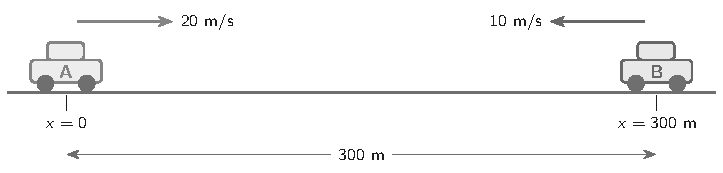
\includegraphics[max width=0.92\linewidth,max height=8.5cm]{fis/mov_encuentro}
\end{center}
\altslargas{A los 10 s, a 100 m de la posición inicial de A.}{A los 10 s, a 200 m de la posición inicial de A.}{A los 15 s, a 300 m de la posición inicial de A.}{A los 30 s, a 600 m de la posición inicial de A.}
\solucion{\textbf{Paso 1. ¿Qué nos piden?} El instante y la posición en que los dos autos coinciden.

\textbf{Paso 2. Ecuaciones de itinerario.} Con origen en la posición inicial de A y positivo hacia la derecha: $x_A = 20t$ y $x_B = 300 - 10t$ (B va en sentido negativo).

\textbf{Paso 3. Iguala.} $20t = 300 - 10t \Rightarrow 30t = 300 \Rightarrow t = 10$ s.

\textbf{Paso 4. Posición.} $x_A = 20\cdot 10 = 200$ m. Comprobación: $x_B = 300 - 100 = 200$ m. \ding{52}

\textbf{Respuesta:} a los 10 s, a 200 m de la posición inicial de A.

\textbf{¿Por qué no las otras?} 100 m es la distancia que recorre B, no la posición del encuentro medida desde A. 15 s es el tiempo que tardaría A en llegar a 300 m si B estuviera detenido. 30 s resta las rapideces, como si B fuera en el mismo sentido que A.

\textbf{\color{cienciaD}Para recordar.} Encuentro: iguala las ecuaciones de itinerario con un solo origen para ambos móviles.}{B}
\end{elejemplo}

%% =====================================================================
%% fis_mrua
\section[Movimiento rectilíneo uniformemente acelerado]{Movimiento rectilíneo uniformemente acelerado}
\modcomun\ \ {\color{gris}\itshape Movimiento en línea recta con aceleración constante: ecuaciones v(t) = v0 + a t y x(t) = x0 + v0 t + ½ a t², gráficos x--t (parábola), v--t (pendiente y área) y a--t, caída libre y lanzamiento vertical con g = 10 m/s², y distancia de frenado.\par}
\subsection{Movimiento con aceleración constante}
Un cuerpo tiene \textbf{movimiento rectilíneo uniformemente acelerado (MRUA)} cuando se mueve en línea recta con \textbf{aceleración constante}: su velocidad cambia en la misma cantidad cada segundo.

 
\begin{center}
$v(t) = v_0 + a\,t$
\end{center}
 

Por ejemplo, un auto que parte del reposo con $a = 2$ m/s²:

 
\begin{center}\small
\begin{tabular}{@{}llllll@{}}
\toprule
\textbf{$t$ (s)} & \textbf{0} & \textbf{1} & \textbf{2} & \textbf{3} & \textbf{4} \\
\midrule
\textbf{$v$ (m/s)} & 0 & 2 & 4 & 6 & 8 \\
\bottomrule
\end{tabular}
\end{center}
 

Si $a$ y $v$ tienen el \textbf{mismo signo}, la rapidez aumenta. Si tienen \textbf{signos opuestos}, la rapidez disminuye: el cuerpo frena hasta detenerse y, si la aceleración sigue actuando, empieza a moverse en sentido contrario.

  
\begin{clave}[{Recuerda}] Frenar no siempre significa aceleración negativa: significa que la aceleración y la velocidad tienen signos opuestos. Un auto que retrocede ($v < 0$) y frena tiene aceleración positiva.\end{clave}
 
\begin{clave}[{Recuerda}] La aceleración de un MRUA es constante, pero su velocidad cambia. Si un problema dice «parte del reposo», entonces $v_0 = 0$; si dice «se detiene», entonces la velocidad final es 0.\end{clave}
\subsection{Ecuación de itinerario del MRUA}
La posición en cada instante es:

 
\begin{center}
$x(t) = x_0 + v_0\,t + \tfrac{1}{2}\,a\,t^2$
\end{center}
 

Si parte del reposo desde el origen, queda $x = \tfrac{1}{2}\,a\,t^2$. Con $a = 4$ m/s², en 3 s recorre $\tfrac{1}{2}\cdot 4\cdot 9 = 18$ m.

 

Dos relaciones útiles que salen de las anteriores:

 
\begin{itemize}
  \item Velocidad media: $\Delta x = \dfrac{v_0 + v}{2}\,t$.
  \item Sin el tiempo: $v^2 = v_0^2 + 2\,a\,\Delta x$.
\end{itemize}
  
\begin{clave}[{Recuerda}] No olvides el $\tfrac{1}{2}$: en $x(t) = 5 + 2t + 3t^2$, el coeficiente de $t^2$ es $\tfrac{a}{2} = 3$, así que $a = 6$ m/s². Además, $x_0 = 5$ m y $v_0 = 2$ m/s.\end{clave}
 
\begin{clave}[{Distancias en segundos sucesivos}] Partiendo del reposo, lo que se recorre en el 1.º, 2.º, 3.º y 4.º segundo crece como 1 : 3 : 5 : 7. Con $a = 2$ m/s²: 1 m, 3 m, 5 m y 7 m. Si las distancias en intervalos iguales aumentan siempre en la misma cantidad, el movimiento es uniformemente acelerado.\end{clave}
\subsection{Gráficos del MRUA}
\begin{center}
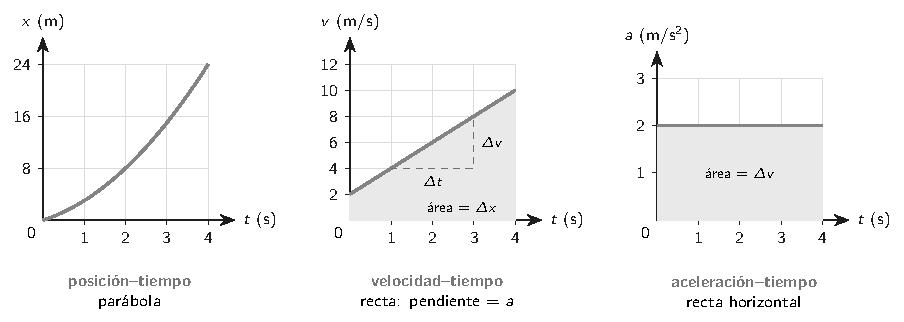
\includegraphics[max width=0.92\linewidth,max height=8.5cm]{fis/mov_mrua_graficos}
\end{center}
  

\textbf{$x$--$t$:} una \textbf{parábola}. Su pendiente, que es la velocidad, cambia: si la curva se empina, el cuerpo va cada vez más rápido.

 

\textbf{$v$--$t$:} una \textbf{recta inclinada}. Corta el eje vertical en $v_0$; su \textbf{pendiente es la aceleración}: $a = \dfrac{\Delta v}{\Delta t} = \dfrac{10 - 2}{4} = 2$ m/s².

  

El \textbf{área bajo $v$--$t$} es el desplazamiento. Aquí es un trapecio: $\Delta x = \dfrac{2 + 10}{2}\cdot 4 = 24$ m, igual que en el gráfico $x$--$t$.

 

\textbf{$a$--$t$:} una \textbf{recta horizontal}. El área bajo ella es el cambio de velocidad: $2\cdot 4 = 8$ m/s.
\subsection{Caída libre y lanzamiento vertical}
Si el roce con el aire es despreciable, todos los cuerpos caen con la misma aceleración, la \textbf{aceleración de gravedad}: $g = 10$ m/s², dirigida hacia abajo. No depende de la masa: un martillo y una pluma soltados en la Luna llegan al suelo al mismo tiempo.

 

Para un cuerpo que se suelta desde el reposo:

 
\begin{center}
$v = g\,t \qquad h = \tfrac{1}{2}\,g\,t^2$
\end{center}
 

\textbf{Lanzamiento hacia arriba.} El cuerpo sube cada vez más lento, se detiene un instante en el punto más alto y luego cae. Durante todo el movimiento su aceleración es $g$ hacia abajo, también en el punto más alto. Si se lanza con $v_0 = 20$ m/s:

 
\begin{itemize}
  \item tiempo de subida: $\dfrac{v_0}{g} = 2$ s, y otros 2 s de bajada;
  \item altura máxima: $\dfrac{v_0^2}{2g} = \dfrac{400}{20} = 20$ m.
\end{itemize}
  
\begin{center}
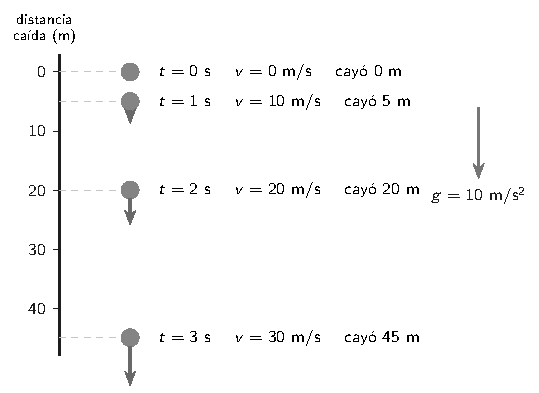
\includegraphics[max width=0.92\linewidth,max height=8.5cm]{fis/mov_caida}
\end{center}
 
\begin{clave}[{Recuerda}] En el punto más alto la velocidad es nula, pero la aceleración no: sigue siendo 10 m/s² hacia abajo. Si la aceleración fuera nula, el cuerpo se quedaría flotando allí.\end{clave}
\subsection{Frenado y distancia de detención}
Cuando un conductor ve un obstáculo, el auto no empieza a frenar de inmediato:

 
\begin{itemize}
  \item \textbf{Tiempo de reacción} (alrededor de 1 s): el auto sigue con la misma velocidad, en MRU.
  \item \textbf{Frenado}: el auto disminuye su velocidad con aceleración constante hasta detenerse, en MRUA.
\end{itemize}
 

\textbf{Ejemplo.} Un auto a 30 m/s, con 1 s de reacción y una aceleración de frenado de 6 m/s²:

 
\begin{itemize}
  \item reacción: $30\cdot 1 = 30$ m;
  \item frenado: de $0 = 30^2 - 2\cdot 6\cdot d$ resulta $d = \dfrac{900}{12} = 75$ m;
  \item distancia total de detención: 105 m.
\end{itemize}
  
\begin{clave}[{La distancia de frenado crece con el cuadrado de la rapidez}] Como $d = \dfrac{v_0^2}{2a}$, con la misma aceleración de frenado, al duplicar la rapidez la distancia de frenado se cuadruplica, y al triplicarla se multiplica por 9. Por eso los límites de velocidad importan tanto.\end{clave}
 
\begin{clave}[{Recuerda}] En un gráfico $v$--$t$ de frenado, la recta baja hasta $v = 0$. La pendiente es la aceleración (negativa si el auto avanzaba en sentido positivo) y el área bajo la recta es la distancia recorrida mientras frena.\end{clave}
\subsection{Lo clave del tema}
\begin{center}\small
\begin{tabularx}{\linewidth}{@{}>{\raggedright\arraybackslash\hsize=0.89\hsize}X>{\raggedright\arraybackslash\hsize=0.68\hsize}X>{\raggedright\arraybackslash\hsize=1.44\hsize}X@{}}
\toprule
 & \textbf{MRU} & \textbf{MRUA} \\
\midrule
Aceleración & $a = 0$ & $a$ constante, distinta de 0 \\
Velocidad & constante & $v = v_0 + a\,t$ \\
Posición & $x = x_0 + v\,t$ & $x = x_0 + v_0\,t + \tfrac{1}{2}\,a\,t^2$ \\
Gráfico $x$--$t$ & recta & parábola \\
Gráfico $v$--$t$ & recta horizontal & recta inclinada: pendiente = $a$ \\
Gráfico $a$--$t$ & sobre el eje & recta horizontal \\
Área bajo $v$--$t$ & \multicolumn{2}{@{}l@{}}{desplazamiento} \\
Caída libre & \multicolumn{2}{@{}l@{}}{MRUA con $g = 10$ m/s² hacia abajo: $v = g\,t$, $h = \tfrac{1}{2}\,g\,t^2$} \\
\bottomrule
\end{tabularx}
\end{center}
 
\begin{clave}[{Recuerda}] · No olvides el $\tfrac{1}{2}$ en $\tfrac{1}{2}\,a\,t^2$.\par · Sin roce del aire, todos los cuerpos caen con la misma aceleración, sin importar su masa.\par · En el punto más alto de un lanzamiento vertical, $v = 0$ pero $a = g$.\par · Con la misma aceleración de frenado, el doble de rapidez implica cuatro veces la distancia de frenado.\end{clave}
 
\begin{clave}[{Método PAES}] 1. Anota los datos con signo: $x_0$, $v_0$, $a$, $t$. 2. Traduce las frases: «parte del reposo» es $v_0 = 0$ y «se detiene» es $v = 0$. 3. Elige la ecuación que tenga solo una incógnita. 4. En gráficos $v$--$t$, usa la pendiente para la aceleración y el área para el desplazamiento.\end{clave}
\begin{elejemplo}{Estilo PAES}
Un conductor que viaja a 20 m/s por una calle recta ve un obstáculo y frena hasta detenerse. El gráfico muestra la velocidad del auto desde el instante en que el conductor ve el obstáculo.

¿Qué distancia recorre el auto desde que el conductor ve el obstáculo hasta que se detiene, y cuál es su aceleración mientras frena?
\begin{center}
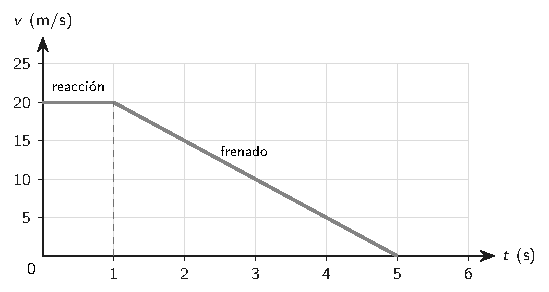
\includegraphics[max width=0.92\linewidth,max height=8.5cm]{fis/mov_frenado}
\end{center}
\alts{60 m y \ensuremath{-}5 m/s²}{40 m y \ensuremath{-}5 m/s²}{100 m y \ensuremath{-}4 m/s²}{60 m y \ensuremath{-}4 m/s²}
\solucion{\textbf{Paso 1. ¿Qué nos piden?} La distancia total (área bajo el gráfico) y la aceleración del frenado (pendiente del segundo tramo).

\textbf{Paso 2. Tramo de reacción.} De 0 a 1 s, velocidad constante de 20 m/s: área $= 20\cdot 1 = 20$ m.

\textbf{Paso 3. Tramo de frenado.} De 1 a 5 s, un triángulo: área $= \dfrac{4\cdot 20}{2} = 40$ m.

\textbf{Paso 4. Distancia total.} $20 + 40 = 60$ m.

\textbf{Paso 5. Aceleración del frenado.} $a = \dfrac{\Delta v}{\Delta t} = \dfrac{0 - 20}{5 - 1} = -5$ m/s². El signo negativo indica que la aceleración es contraria a la velocidad.

\textbf{Respuesta:} 60 m y \ensuremath{-}5 m/s².

\textbf{¿Por qué no las otras?} 40 m cuenta solo el frenado y olvida el tramo de reacción. 100 m multiplica 20 m/s por 5 s, como si el auto nunca hubiera frenado. \ensuremath{-}4 m/s² divide el cambio de velocidad por los 5 s totales, pero el frenado dura 4 s.

\textbf{\color{cienciaD}Para recordar.} En v--t: área = distancia recorrida; pendiente = aceleración.}{A}
\end{elejemplo}

%% =====================================================================
%% fis_newton
\section[Leyes de Newton]{Leyes de Newton}
\modcomun\ \ {\color{gris}\itshape Fuerza y fuerza neta, principio de inercia, relación entre fuerza neta, masa y aceleración, y pares de acción y reacción. Cuerpos con velocidad constante o con aceleración constante, y cómo dibujar e interpretar un diagrama de cuerpo libre.\par}
\subsection{Fuerza y fuerza neta}
Una \textbf{fuerza} es una \textbf{interacción} entre dos cuerpos: uno empuja, tira o atrae al otro. Una fuerza puede cambiar el estado de movimiento de un cuerpo (ponerlo en marcha, frenarlo, desviarlo) o deformarlo.

 

La fuerza es una magnitud \textbf{vectorial}: tiene magnitud, dirección y sentido. Se mide en \textbf{newton} (N) con un \textbf{dinamómetro}: $1\ \text{N} = 1\ \text{kg}\cdot\text{m/s}^2$.

 

Sobre un cuerpo suelen actuar varias fuerzas a la vez. La \textbf{fuerza neta} (o resultante) es su suma vectorial:

 
\begin{itemize}
  \item \textbf{Misma dirección y sentido:} se suman. 30 N y 10 N hacia la derecha dan 40 N hacia la derecha.
  \item \textbf{Misma dirección y sentido contrario:} se restan, y la neta apunta hacia la mayor. 30 N a la derecha y 10 N a la izquierda dan 20 N a la derecha.
  \item \textbf{Fuerzas perpendiculares:} se analizan por separado en cada eje (horizontal y vertical).
\end{itemize}
  
\begin{clave}[{Las fuerzas de esta unidad}] · \textbf{Peso:} la Tierra atrae al cuerpo.\par · \textbf{Normal:} una superficie empuja al cuerpo que se apoya en ella.\par · \textbf{Tensión:} una cuerda tira del cuerpo.\par · \textbf{Fuerza elástica:} un resorte deformado empuja o tira.\par · \textbf{Roce:} una superficie, o el aire, se opone al deslizamiento.\end{clave}
 
\begin{clave}[{Recuerda}] Toda fuerza la ejerce \textbf{un cuerpo sobre otro}. Si no puedes decir qué cuerpo la ejerce, esa fuerza no existe. No hay una «fuerza del movimiento» ni una «fuerza de la inercia».\end{clave}
\subsection{Primera ley: el principio de inercia}
\textbf{Primera ley de Newton.} Si la fuerza neta sobre un cuerpo es cero, el cuerpo mantiene su estado de movimiento: si estaba en reposo, sigue en reposo; si se movía, sigue con \textbf{velocidad constante}, es decir, en línea recta y con la misma rapidez.

 

La \textbf{inercia} es la tendencia de los cuerpos a mantener su velocidad. La \textbf{masa} mide cuánta inercia tiene un cuerpo: cuesta más cambiar la velocidad de un camión que la de una bicicleta.

 

\textbf{Ejemplos.} Cuando un bus frena de golpe, los pasajeros se van hacia adelante: nada los empuja, simplemente siguen moviéndose mientras el bus se detiene. Una sonda en el espacio, lejos de todo planeta, sigue avanzando con los motores apagados.

 
\begin{center}\small
\begin{tabular}{@{}ll@{}}
\toprule
\textbf{Estado del cuerpo} & \textbf{Fuerza neta} \\
\midrule
Reposo & cero \\
Velocidad constante (MRU) & cero \\
La velocidad cambia (rapidez o dirección) & distinta de cero \\
\bottomrule
\end{tabular}
\end{center}
  
\begin{clave}[{Velocidad constante no significa «sin fuerzas»}] Un auto que avanza a 90 km/h constantes por una carretera recta tiene varias fuerzas encima: la que lo impulsa (el roce del camino sobre las ruedas motrices), el roce con el aire, el peso y la normal. Lo que ocurre es que se \textbf{equilibran}: la fuerza neta es cero.\end{clave}
 
\begin{clave}[{Recuerda}] Para mantener un cuerpo en movimiento no se necesita una fuerza neta. En la vida diaria parece que sí, porque el roce frena todo: si empujas un carro y lo sueltas, se detiene por el roce, no porque «se le acabe la fuerza».\end{clave}
\subsection{Segunda ley: fuerza neta, masa y aceleración}
\textbf{Segunda ley de Newton.} La fuerza neta sobre un cuerpo es igual al producto de su masa por su aceleración:

 \[ \vec F_{\text{neta}} = m\,\vec a \] 

La aceleración tiene la \textbf{misma dirección y sentido que la fuerza neta}, no necesariamente que la velocidad. Si la fuerza neta apunta en contra del movimiento, el cuerpo frena.

 
\begin{itemize}
  \item Con la misma masa, el doble de fuerza neta produce el doble de aceleración (proporcionalidad directa).
  \item Con la misma fuerza neta, el doble de masa produce la mitad de aceleración (proporcionalidad inversa).
  \item Fuerza neta constante produce aceleración constante (MRUA).
\end{itemize}
 
\begin{ejemplo}[{Ejemplo resuelto}] Sobre un carro de 4 kg, en un piso sin roce, actúan 30 N hacia la derecha y 10 N hacia la izquierda.\par \textbf{Paso 1.} $F_{\text{neta}} = 30 - 10 = 20$ N hacia la derecha.\par \textbf{Paso 2.} $a = \dfrac{F_{\text{neta}}}{m} = \dfrac{20}{4} = 5\ \text{m/s}^2$ hacia la derecha.\end{ejemplo}
  
\begin{center}
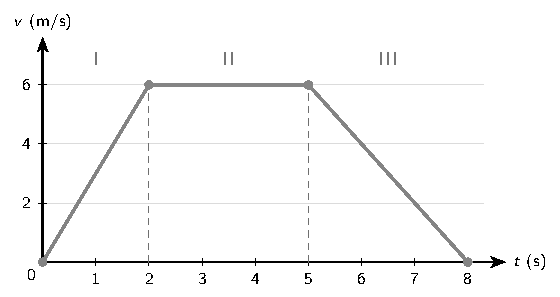
\includegraphics[max width=0.92\linewidth,max height=8.5cm]{fis/fza_vt_newton}
\end{center}
 
\begin{clave}[{Leer la fuerza neta en un gráfico v--t}] La pendiente del gráfico es la aceleración. En el tramo I la rapidez aumenta: la fuerza neta apunta en el sentido del movimiento. En el tramo II la rapidez es constante: la fuerza neta es cero. En el tramo III la rapidez disminuye: la fuerza neta apunta en contra del movimiento.\end{clave}
\subsection{Tercera ley: acción y reacción}
\textbf{Tercera ley de Newton.} Si un cuerpo A ejerce una fuerza sobre un cuerpo B, entonces B ejerce sobre A una fuerza de \textbf{igual magnitud}, \textbf{igual dirección} y \textbf{sentido contrario}. Las fuerzas siempre aparecen de a pares.

 

Características de un par de acción y reacción:

 
\begin{itemize}
  \item Actúan sobre \textbf{cuerpos distintos}; por eso \textbf{nunca se anulan} entre sí.
  \item Son del mismo tipo: ambas de contacto, o ambas gravitacionales.
  \item Aparecen y desaparecen al mismo tiempo.
\end{itemize}
 

\textbf{Ejemplos.} Al caminar empujas el suelo hacia atrás, y el suelo te empuja hacia adelante. Un cohete empuja los gases hacia abajo, y los gases empujan al cohete hacia arriba. Si un camión choca con un auto, ambos reciben fuerzas de igual magnitud; el auto, de menor masa, sufre una aceleración mucho mayor.

  
\begin{center}
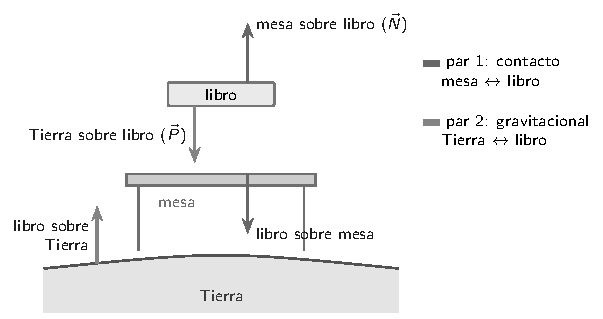
\includegraphics[max width=0.92\linewidth,max height=8.5cm]{fis/fza_pares}
\end{center}
 
\begin{clave}[{Recuerda}] El peso y la normal de un libro sobre una mesa tienen igual magnitud y sentido contrario, pero \textbf{no} son un par de acción y reacción: las dos actúan sobre el libro y son de distinto tipo. La reacción del peso es la fuerza con que el libro atrae a la Tierra; la reacción de la normal es la fuerza con que el libro empuja a la mesa.\end{clave}
\subsection{Diagrama de cuerpo libre}
Un \textbf{diagrama de cuerpo libre} (DCL) muestra todas las fuerzas que actúan sobre \textbf{un solo cuerpo}. Para construirlo:

 
\begin{enumerate}
  \item Elige el cuerpo y sepáralo mentalmente de todo lo que lo rodea.
  \item Represéntalo como un punto.
  \item Dibuja el \textbf{peso}, siempre vertical hacia abajo.
  \item Revisa qué toca al cuerpo: cada contacto puede aportar una fuerza (normal y roce de una superficie, tensión de una cuerda, empuje de una mano).
  \item Dibuja cada flecha con un largo proporcional a su magnitud.
\end{enumerate}
 

Después aplica Newton \textbf{por ejes}. Si el bloque de la figura se mueve con velocidad constante, en el eje vertical $N = P$ y en el horizontal $F = f_r$. Si $F > f_r$, acelera hacia la derecha.

  
\begin{center}
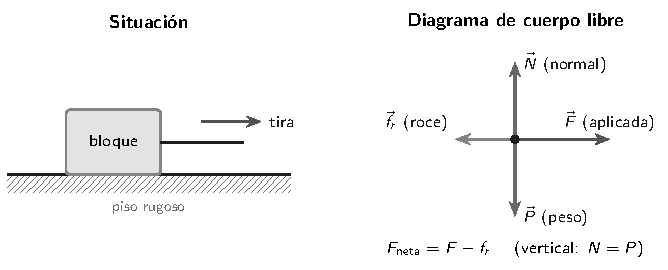
\includegraphics[max width=0.92\linewidth,max height=8.5cm]{fis/fza_dcl_bloque}
\end{center}
 
\begin{clave}[{Recuerda}] En el DCL van solo las fuerzas que \textbf{otros cuerpos ejercen sobre el cuerpo elegido}. No dibujes las fuerzas que el cuerpo ejerce sobre otros, ni $m\vec a$ como si fuera una fuerza más.\end{clave}
\subsection{Lo clave del tema}
\begin{center}\small
\begin{tabularx}{\linewidth}{@{}>{\raggedright\arraybackslash\hsize=0.76\hsize}X>{\raggedright\arraybackslash\hsize=1.12\hsize}X>{\raggedright\arraybackslash\hsize=1.12\hsize}X@{}}
\toprule
\textbf{Ley} & \textbf{Enunciado} & \textbf{Cómo se usa en la PAES} \\
\midrule
Primera (inercia) & fuerza neta cero: reposo o velocidad constante & velocidad constante indica fuerzas equilibradas \\
Segunda & $\vec F_{\text{neta}} = m\,\vec a$ & calcular la aceleración o la fuerza; la aceleración apunta como la fuerza neta \\
Tercera (acción y reacción) & fuerzas de igual magnitud y sentido contrario, sobre cuerpos distintos & choques, caminar, cohetes; los pares no se anulan \\
Diagrama de cuerpo libre & solo las fuerzas que actúan sobre el cuerpo & sumar las fuerzas por ejes \\
\bottomrule
\end{tabularx}
\end{center}
 
\begin{clave}[{Recuerda}] · Velocidad constante no significa ausencia de fuerzas: significa fuerza neta cero.\par · La aceleración, no la velocidad, tiene el sentido de la fuerza neta.\par · El peso y la normal no son un par de acción y reacción.\par · En un gráfico v--t, la pendiente es la aceleración; por la masa da la fuerza neta.\end{clave}
 
\begin{clave}[{Método PAES}] 1. Elige el cuerpo y haz su DCL. 2. Decide si su velocidad es constante o cambia. 3. Si es constante, iguala las fuerzas en cada eje; si cambia, usa $F_{\text{neta}} = m\,a$. 4. En preguntas de acción y reacción, revisa sobre qué cuerpo actúa cada fuerza. 5. Descarta las alternativas que inventan fuerzas sin un cuerpo que las ejerza.\end{clave}
\begin{elejemplo}{Estilo PAES}
Un carro de 2 kg se mueve en línea recta sobre una superficie horizontal. El gráfico muestra su rapidez en función del tiempo.

¿Cuál de las siguientes afirmaciones sobre la fuerza neta que actúa sobre el carro es correcta?
\begin{center}
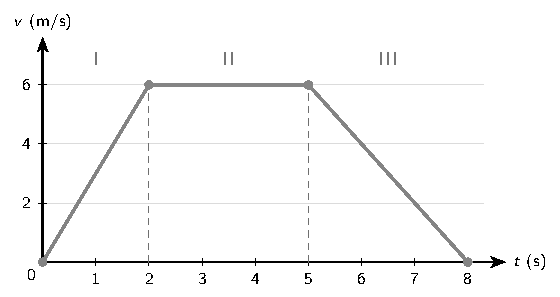
\includegraphics[max width=0.92\linewidth,max height=8.5cm]{fis/fza_vt_newton}
\end{center}
\altslargas{Entre 0 s y 2 s la fuerza neta es de 12 N, y entre 2 s y 5 s es nula.}{Entre 0 s y 2 s la fuerza neta es de 6 N, y entre 2 s y 5 s es nula.}{Entre 2 s y 5 s no actúa ninguna fuerza sobre el carro.}{Entre 5 s y 8 s la fuerza neta tiene el mismo sentido que el movimiento.}
\solucion{\textbf{Paso 1. ¿Qué nos piden?} La fuerza neta sobre el carro en cada tramo, a partir de un gráfico de rapidez en función del tiempo.

\textbf{Paso 2. Calcula la aceleración de cada tramo.} La aceleración es la pendiente del gráfico. Entre 0 y 2 s: $a = \dfrac{6 - 0}{2 - 0} = 3\ \text{m/s}^2$. Entre 2 y 5 s la rapidez no cambia: $a = 0$. Entre 5 y 8 s: $a = \dfrac{0 - 6}{8 - 5} = -2\ \text{m/s}^2$.

\textbf{Paso 3. Aplica la segunda ley.} $F_{\text{neta}} = m\,a$. Entre 0 y 2 s: $2\cdot 3 = 6$ N. Entre 2 y 5 s: $2\cdot 0 = 0$. Entre 5 y 8 s: $2\cdot 2 = 4$ N, en contra del movimiento.

\textbf{Respuesta:} entre 0 s y 2 s la fuerza neta es de 6 N, y entre 2 s y 5 s es nula.

\textbf{¿Por qué no las otras?} 12 N sale de multiplicar la masa por la rapidez (2 · 6), y la segunda ley usa la aceleración. Que la fuerza neta sea nula no significa que no haya fuerzas: sobre el carro actúan al menos el peso y la normal, que se equilibran. Entre 5 y 8 s el carro frena, así que la aceleración, y con ella la fuerza neta, apunta en contra del movimiento.

\textbf{\color{cienciaD}Para recordar.} La pendiente del gráfico v--t es la aceleración; multiplicada por la masa da la fuerza neta.}{B}
\end{elejemplo}

%% =====================================================================
%% fis_fuerzas
\section[Peso, normal, tensión y fuerza elástica]{Peso, normal, tensión y fuerza elástica}
\modcomun\ \ {\color{gris}\itshape Las fuerzas más comunes: peso (masa frente a peso, otros planetas), normal, tensión en cuerdas y poleas, y fuerza elástica con la ley de Hooke y sus gráficos. Problemas con diagrama de cuerpo libre en superficies horizontales.\par}
\subsection{Masa y peso}
La \textbf{masa} ($m$) mide la cantidad de materia de un cuerpo y su inercia. Se mide en kilogramos (kg) con una \textbf{balanza}, y es la misma en cualquier lugar del universo.

 

El \textbf{peso} ($\vec P$) es la fuerza con que un planeta, u otro astro, atrae a un cuerpo. Es vertical, apunta hacia el centro del planeta y se mide en newton (N) con un \textbf{dinamómetro}:

 \[ P = m\,g \] 

donde $g$ es la aceleración de gravedad del lugar: cerca de $10\ \text{m/s}^2$ en la Tierra, $1{,}6\ \text{m/s}^2$ en la Luna y $3{,}7\ \text{m/s}^2$ en Marte.

  
\begin{center}\small
\begin{tabular}{@{}llll@{}}
\toprule
\textbf{Lugar} & \textbf{$g$ (m/s²)} & \textbf{Masa} & \textbf{Peso} \\
\midrule
Tierra & 10 & 60 kg & 600 N \\
Marte & 3,7 & 60 kg & 222 N \\
Luna & 1,6 & 60 kg & 96 N \\
\bottomrule
\end{tabular}
\end{center}
 
\begin{clave}[{Recuerda}] En la vida diaria decimos «peso 60 kilos», pero en física esa cantidad es la masa. Tu peso en la Tierra es de unos 600 N. Si viajas a la Luna, tu masa no cambia; tu peso se reduce a cerca de la sexta parte.\end{clave}
\subsection{Fuerza normal}
La \textbf{normal} ($\vec N$) es la fuerza que ejerce una superficie sobre un cuerpo apoyado en ella. Es \textbf{perpendicular} a la superficie y empuja hacia afuera de ella. Solo existe si hay contacto.

 

La normal se ajusta a cada situación: \textbf{no siempre es igual al peso}. Para encontrarla, haz el DCL y aplica Newton en la dirección perpendicular a la superficie.

 
\begin{center}\small
\begin{tabular}{@{}ll@{}}
\toprule
\textbf{Cuerpo en reposo sobre un piso horizontal} & \textbf{Normal} \\
\midrule
solo actúan el peso y la normal & $N = P$ \\
lo empujas hacia abajo con una fuerza $F$ & $N = P + F$ \\
tiras de él hacia arriba con $F$, sin levantarlo & $N = P - F$ \\
tiene encima otro cuerpo de peso $P_2$ & $N = P + P_2$ \\
\bottomrule
\end{tabular}
\end{center}
 

En un plano inclinado, la normal es menor que el peso.

  
\begin{ejemplo}[{Ejemplo resuelto}] Una caja de 5 kg está en el piso y tiras de ella hacia arriba con 20 N, sin levantarla.\par \textbf{Paso 1.} $P = 5\cdot 10 = 50$ N hacia abajo.\par \textbf{Paso 2.} Hacia arriba actúan tu fuerza y la normal. En reposo: $N + 20 = 50$.\par \textbf{Paso 3.} $N = 30$ N.\end{ejemplo}
 
\begin{clave}[{Recuerda}] El peso y la normal no son un par de acción y reacción: actúan sobre el mismo cuerpo. La reacción de la normal es la fuerza con que el cuerpo empuja a la superficie.\end{clave}
\subsection{Tensión y poleas}
La \textbf{tensión} ($\vec T$) es la fuerza que ejerce una cuerda tensa sobre el cuerpo atado a ella. Siempre \textbf{tira} del cuerpo, a lo largo de la cuerda.

 

En la PAES las cuerdas suelen ser \textbf{ideales}: inextensibles y de masa despreciable. Una cuerda ideal transmite la \textbf{misma tensión} en todos sus puntos.

 

Una \textbf{polea ideal}, sin masa ni roce, solo cambia la dirección de la cuerda: la tensión es la misma a ambos lados.

 

\textbf{Cuerpo que cuelga en reposo o con velocidad constante:} $T = P = m\,g$.

 
\begin{clave}[{Recuerda}] Si la cuerda es gruesa y pesada (no ideal), la tensión es mayor arriba que abajo: la parte superior sostiene, además del cuerpo, el peso de la cuerda que cuelga bajo ella.\end{clave}
  
\begin{center}
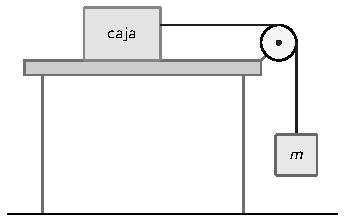
\includegraphics[max width=0.92\linewidth,max height=8.5cm]{fis/fza_polea}
\end{center}
 
\begin{ejemplo}[{Ejemplo resuelto}] En la figura, la caja está en reposo y cuelga un cuerpo de 1,5 kg.\par \textbf{Paso 1.} El cuerpo colgante está en reposo: $T = m\,g = 1{,}5\cdot 10 = 15$ N.\par \textbf{Paso 2.} La cuerda ideal tira de la caja, en horizontal, con los mismos 15 N.\par \textbf{Paso 3.} La caja no se mueve: el roce estático de la mesa sobre ella también vale 15 N.\end{ejemplo}
\subsection{Fuerza elástica: ley de Hooke}
Un resorte estirado o comprimido ejerce una \textbf{fuerza elástica} que tiende a devolverlo a su longitud natural. La \textbf{ley de Hooke} dice que la magnitud de esa fuerza es proporcional a la \textbf{deformación}:

 \[ F = k\,\Delta x \] 
\begin{itemize}
  \item $\Delta x = L - L_0$: cuánto cambió la longitud respecto de la longitud natural $L_0$. No es la longitud total.
  \item $k$: constante elástica, en N/m o N/cm. Un $k$ mayor indica un resorte más rígido, que cuesta más deformar.
  \item El gráfico de $F$ en función de $\Delta x$ es una recta que pasa por el origen, y su \textbf{pendiente es $k$}.
  \item La ley vale hasta el \textbf{límite elástico}. Más allá, el resorte queda deformado y el gráfico deja de ser una recta.
\end{itemize}
 
\begin{ejemplo}[{Ejemplo resuelto}] Con 30 N un resorte se estira 20 cm. ¿Qué fuerza lo estira 45 cm?\par \textbf{Paso 1.} $k = \dfrac{30}{20} = 1{,}5$ N/cm.\par \textbf{Paso 2.} $F = 1{,}5\cdot 45 = 67{,}5$ N.\end{ejemplo}
  
\begin{center}
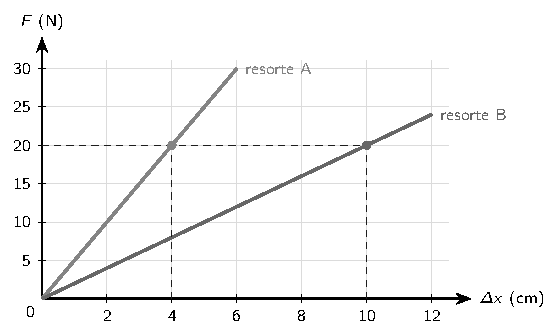
\includegraphics[max width=0.92\linewidth,max height=8.5cm]{fis/fza_hooke_grafico}
\end{center}
 
\begin{clave}[{Leer el gráfico}] Con 20 N, el resorte A se deforma 4 cm y el B, 10 cm. Entonces $k_A = \dfrac{20}{4} = 5$ N/cm y $k_B = \dfrac{20}{10} = 2$ N/cm. El resorte A es más rígido: su recta es más empinada.\end{clave}
\subsection{Lo clave del tema}
\begin{center}\small
\begin{tabularx}{\linewidth}{@{}>{\raggedright\arraybackslash\hsize=0.42\hsize}X>{\raggedright\arraybackslash\hsize=0.84\hsize}X>{\raggedright\arraybackslash\hsize=1.22\hsize}X>{\raggedright\arraybackslash\hsize=1.52\hsize}X@{}}
\toprule
\textbf{Fuerza} & \textbf{Quién la ejerce} & \textbf{Dirección} & \textbf{Cómo se calcula} \\
\midrule
Peso & el planeta & vertical, hacia abajo & $P = m\,g$ \\
Normal & la superficie de apoyo & perpendicular a la superficie & con el DCL; no siempre es igual al peso \\
Tensión & una cuerda & a lo largo de la cuerda, tirando & con el DCL; igual en toda una cuerda ideal \\
Elástica & un resorte & hacia la longitud natural & $F = k\,\Delta x$ \\
\bottomrule
\end{tabularx}
\end{center}
 
\begin{clave}[{Recuerda}] · La masa no cambia de un planeta a otro; el peso sí.\par · En la ley de Hooke se usa la deformación $\Delta x$, no la longitud total.\par · La pendiente del gráfico $F$--$\Delta x$ es la constante $k$.\end{clave}
 
\begin{clave}[{Método PAES}] 1. Haz el DCL del cuerpo. 2. Calcula el peso con $P = m\,g$. 3. Decide si la aceleración es cero o no, y hacia dónde apunta. 4. Plantea la suma de fuerzas en el eje que corresponda. 5. En resortes, convierte longitudes en deformaciones antes de usar $F = k\,\Delta x$.\end{clave}
\begin{elejemplo}{Estilo PAES}
El gráfico muestra la fuerza aplicada en función de la deformación para dos resortes, A y B.

¿Cuál de las siguientes afirmaciones es correcta?
\begin{center}
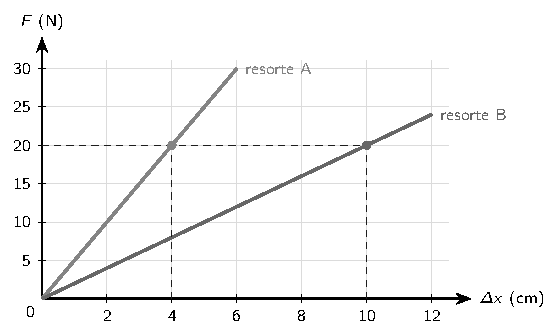
\includegraphics[max width=0.92\linewidth,max height=8.5cm]{fis/fza_hooke_grafico}
\end{center}
\altslargas{El resorte B es más rígido, porque se estira más con la misma fuerza.}{Ambos resortes tienen la misma constante, porque sus gráficos son rectas que pasan por el origen.}{La constante del resorte A es 0,2 N/cm.}{El resorte A es más rígido: su constante es 5 N/cm y la de B es 2 N/cm.}
\solucion{\textbf{Paso 1. ¿Qué nos piden?} Comparar las constantes elásticas a partir del gráfico.

\textbf{Paso 2. Lee un punto de cada recta.} Con 20 N, A se deforma 4 cm y B se deforma 10 cm.

\textbf{Paso 3. Calcula las pendientes.} $k_A = \dfrac{20}{4} = 5$ N/cm y $k_B = \dfrac{20}{10} = 2$ N/cm. A necesita más fuerza por cada centímetro: es más rígido.

\textbf{Respuesta:} A es más rígido: su constante es 5 N/cm y la de B es 2 N/cm.

\textbf{¿Por qué no las otras?} Estirarse más con la misma fuerza indica un resorte más blando, no más rígido. Que ambos gráficos sean rectas por el origen indica que ambos cumplen la ley de Hooke, pero sus pendientes son distintas. 0,2 sale de dividir la deformación por la fuerza ($\dfrac{4}{20}$), al revés.

\textbf{\color{cienciaD}Para recordar.} En el gráfico F--\ensuremath{\Delta}x, la recta más empinada es la del resorte más rígido.}{D}
\end{elejemplo}

%% =====================================================================
%% fis_roce
\section[Fuerza de roce]{Fuerza de roce}
\modcomun\ \ {\color{gris}\itshape Roce estático (hasta su valor máximo \ensuremath{\mu}s N) y roce cinético (\ensuremath{\mu}k N), su dependencia de las superficies y de la normal, y la lectura de gráficos de roce en función de la fuerza aplicada. Roce con el aire en términos cualitativos: velocidad límite y paracaídas.\par}
\subsection{Qué es la fuerza de roce}
La \textbf{fuerza de roce} ($\vec f_r$) aparece cuando dos superficies en contacto deslizan, o tienden a deslizar, una sobre otra. Es \textbf{paralela} a las superficies y se \textbf{opone al deslizamiento}, o a la tendencia a deslizar.

 

Se origina en las irregularidades microscópicas de las superficies, que se traban y se adhieren entre sí. Incluso una superficie que parece lisa es rugosa vista al microscopio.

 

Su magnitud depende de:

 
\begin{itemize}
  \item el \textbf{tipo de superficies} en contacto (madera sobre cemento, goma sobre asfalto, acero sobre hielo), que se resume en un \textbf{coeficiente de roce} $\mu$, sin unidad;
  \item la \textbf{fuerza normal}: mientras más se aprietan las superficies, mayor es el roce.
\end{itemize}
 

En el modelo que usa la PAES, el roce entre sólidos \textbf{no depende del área de contacto} ni de la rapidez del deslizamiento.

  
\begin{clave}[{Útil y perjudicial}] Sin roce no podrías caminar, los autos no podrían frenar ni doblar y los clavos se soltarían. Pero el roce también desgasta piezas y transforma energía en calor: por eso se usan lubricantes y rodamientos en las máquinas.\end{clave}
 
\begin{clave}[{Recuerda}] El roce se opone al deslizamiento entre las superficies, no siempre al movimiento del cuerpo. Cuando caminas, tu pie empuja el suelo hacia atrás, y el roce del suelo sobre tu zapato apunta hacia adelante: es la fuerza que te impulsa.\end{clave}
\subsection{Roce estático}
Mientras el cuerpo está \textbf{en reposo} respecto de la superficie, actúa el \textbf{roce estático}. Su magnitud no es fija: toma el valor justo para impedir el deslizamiento, igual a la fuerza que tiende a mover el cuerpo.

 

Pero tiene un tope. El roce estático máximo es:

 \[ f_{s,\text{máx}} = \mu_s\,N \] 

donde $\mu_s$ es el coeficiente de roce estático. Si la fuerza aplicada supera ese valor, el cuerpo empieza a deslizar.

 
\begin{clave}[{Recuerda}] El producto $\mu_s\,N$ es el roce estático \textbf{máximo}, no el roce que actúa siempre. Úsalo solo cuando el cuerpo está a punto de deslizar.\end{clave}
  
\begin{ejemplo}[{Ejemplo resuelto}] Un bloque de 2 kg está sobre un piso horizontal, con $\mu_s = 0{,}6$.\par \textbf{Paso 1.} Normal: $N = P = 2\cdot 10 = 20$ N.\par \textbf{Paso 2.} Roce estático máximo: $f_{s,\text{máx}} = 0{,}6\cdot 20 = 12$ N.\par \textbf{Paso 3.} Si lo empujas con 5 N, no se mueve y el roce vale 5 N. Con 10 N, no se mueve y el roce vale 10 N. Con 13 N, se supera el máximo y el bloque empieza a moverse.\end{ejemplo}
 
\begin{center}\small
\begin{tabular}{@{}lll@{}}
\toprule
\textbf{Fuerza aplicada} & \textbf{¿Se mueve?} & \textbf{Roce} \\
\midrule
5 N & no & 5 N (estático) \\
10 N & no & 10 N (estático) \\
12 N & a punto de moverse & 12 N (estático máximo) \\
\bottomrule
\end{tabular}
\end{center}
\subsection{Roce cinético}
Cuando el cuerpo ya \textbf{desliza}, actúa el \textbf{roce cinético}, de magnitud prácticamente constante:

 \[ f_k = \mu_k\,N \] 

Para un mismo par de superficies, $\mu_k < \mu_s$: cuesta más poner un cuerpo en movimiento que mantenerlo deslizando. Por eso, al empujar un mueble, hace falta un empujón fuerte para que parta, y después basta una fuerza menor.

 
\begin{itemize}
  \item Si la fuerza aplicada es igual a $f_k$, la fuerza neta es cero y el cuerpo desliza con \textbf{velocidad constante}.
  \item Si es mayor, el cuerpo acelera: $a = \dfrac{F - f_k}{m}$.
  \item Si deja de aplicarse, el roce lo frena hasta detenerlo, con una aceleración $\dfrac{f_k}{m}$ opuesta al movimiento.
\end{itemize}
  
\begin{ejemplo}[{Ejemplo resuelto}] El mismo bloque de 2 kg, ahora con $\mu_k = 0{,}4$, desliza por el piso.\par \textbf{Paso 1.} $f_k = 0{,}4\cdot 20 = 8$ N.\par \textbf{Paso 2.} Empujado con 12 N: $a = \dfrac{12 - 8}{2} = 2\ \text{m/s}^2$.\par \textbf{Paso 3.} Empujado con 8 N: la fuerza neta es cero y avanza con velocidad constante.\par \textbf{Paso 4.} Si lo sueltas: frena con $a = \dfrac{8}{2} = 4\ \text{m/s}^2$.\end{ejemplo}
 
\begin{clave}[{Recuerda}] El roce cinético no aumenta si empujas más fuerte: depende solo de $\mu_k$ y de la normal. Empujar más fuerte aumenta la aceleración.\end{clave}
\subsection{Gráficos del roce}
\begin{center}
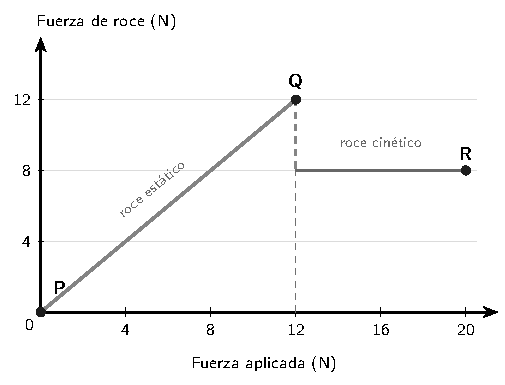
\includegraphics[max width=0.92\linewidth,max height=8.5cm]{fis/fza_roce_grafico}
\end{center}
  

Al aumentar poco a poco la fuerza horizontal aplicada a un bloque en reposo:

 
\begin{itemize}
  \item \textbf{Tramo P--Q:} el bloque sigue en reposo. El roce estático crece junto con la fuerza aplicada y la iguala en todo momento.
  \item \textbf{Punto Q:} se alcanza el roce estático máximo, 12 N, y el bloque empieza a deslizar.
  \item \textbf{Tramo Q--R:} el bloque desliza. El roce es cinético y constante, 8 N, menor que el máximo estático, aunque la fuerza aplicada siga creciendo.
\end{itemize}
 
\begin{clave}[{Recuerda}] En el tramo Q--R el bloque acelera cada vez más, porque la fuerza aplicada crece y el roce se mantiene. Con una fuerza aplicada de 20 N, la fuerza neta es $20 - 8 = 12$ N.\end{clave}
 
\begin{clave}[{Gráficos de fuerza en función del tiempo}] Si el bloque desliza con velocidad constante durante un tramo, en ese tramo la fuerza aplicada es igual al roce cinético. El valor de la fuerza justo cuando el bloque empieza a moverse es el roce estático máximo.\end{clave}
\subsection{Roce con el aire}
Un cuerpo que se mueve en el aire, o en el agua, recibe una fuerza de roce opuesta a su movimiento. A diferencia del roce entre sólidos, este roce \textbf{aumenta con la rapidez}. También aumenta con el \textbf{área} que el cuerpo presenta de frente al avance, y depende de su \textbf{forma}: las formas aerodinámicas lo reducen.

 

\textbf{Caída de un paracaidista} (figura):

 
\begin{itemize}
  \item \textbf{I:} al saltar, el roce es pequeño y la rapidez aumenta. A medida que cae más rápido, el roce crece y la aceleración disminuye.
  \item \textbf{II:} el roce iguala al peso. La fuerza neta es cero y cae con una \textbf{velocidad límite} constante, $v_1$.
  \item \textbf{III:} al abrir el paracaídas, el área aumenta mucho y el roce supera al peso. La fuerza neta apunta hacia arriba y el paracaidista \textbf{frena}.
  \item \textbf{IV:} al frenar, el roce disminuye hasta igualar de nuevo al peso: nueva velocidad límite $v_2$, mucho menor.
\end{itemize}
  
\begin{center}
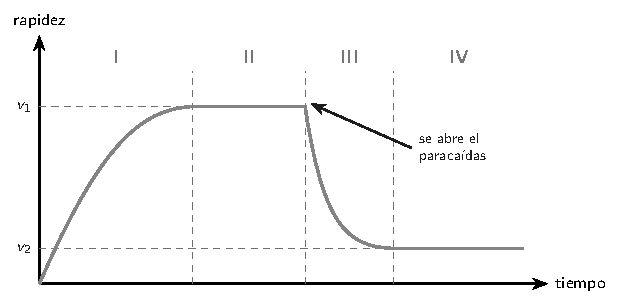
\includegraphics[max width=0.92\linewidth,max height=8.5cm]{fis/fza_paracaidas}
\end{center}
 
\begin{clave}[{Recuerda}] En el vacío, todos los cuerpos caen con la misma aceleración $g$, sin importar su masa. En el aire, una hoja de papel extendida cae más lento que una hoja igual arrugada: tienen la misma masa, pero distinta área frente al aire.\end{clave}
\subsection{Lo clave del tema}
\begin{center}\small
\begin{tabularx}{\linewidth}{@{}>{\raggedright\arraybackslash\hsize=0.37\hsize}X>{\raggedright\arraybackslash\hsize=1.17\hsize}X>{\raggedright\arraybackslash\hsize=1.23\hsize}X>{\raggedright\arraybackslash\hsize=1.23\hsize}X@{}}
\toprule
\textbf{Tipo de roce} & \textbf{Cuándo actúa} & \textbf{Magnitud} & \textbf{Depende de} \\
\midrule
Estático & cuerpo en reposo que tiende a deslizar & igual a la fuerza que tiende a moverlo, hasta $\mu_s\,N$ & superficies y normal \\
Cinético & cuerpo que desliza & $\mu_k\,N$, constante & superficies y normal; no del área ni de la rapidez \\
Con el aire & cuerpo que se mueve en un fluido & crece con la rapidez & rapidez, área y forma \\
\bottomrule
\end{tabularx}
\end{center}
 
\begin{clave}[{Recuerda}] · $\mu_k < \mu_s$: cuesta más hacer partir un cuerpo que mantenerlo deslizando.\par · El roce estático no siempre vale $\mu_s\,N$: ese es su máximo.\par · Con roce y velocidad constante, la fuerza aplicada iguala al roce cinético.\par · Velocidad límite: el roce del aire iguala al peso.\end{clave}
 
\begin{clave}[{Método PAES}] 1. Decide si el cuerpo está en reposo o desliza. 2. Calcula la normal con el DCL. 3. En reposo, el roce iguala a la fuerza que tiende a moverlo (sin pasar de $\mu_s\,N$); deslizando, vale $\mu_k\,N$. 4. Aplica $F_{\text{neta}} = m\,a$. 5. En gráficos, busca dónde empieza el movimiento y dónde la velocidad es constante.\end{clave}
\begin{elejemplo}{PAES Invierno 2026, adaptada}
Un bloque de 2 kg está en reposo sobre una superficie horizontal rugosa. Se le aplica una fuerza horizontal cuya magnitud cambia en el tiempo como muestra el gráfico. El bloque comienza a moverse justo a los 4 s, y entre los 6 s y los 8 s se mueve con velocidad constante.

Si $g = 10\ \text{m/s}^2$, ¿cuáles son los coeficientes de roce estático y cinético entre el bloque y la superficie?
\begin{center}
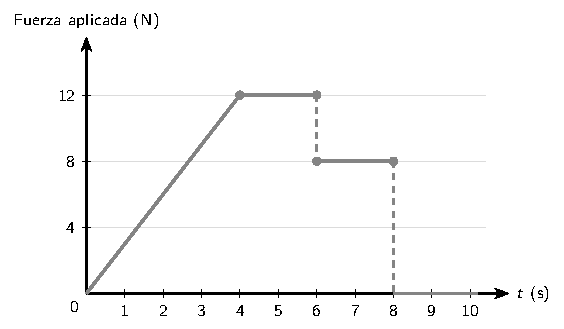
\includegraphics[max width=0.92\linewidth,max height=8.5cm]{fis/fza_fuerza_tiempo}
\end{center}
\alts{$\mu_s = 0{,}4$ y $\mu_k = 0{,}6$}{$\mu_s = 6$ y $\mu_k = 4$}{$\mu_s = 0{,}6$ y $\mu_k = 0{,}4$}{$\mu_s = 0{,}6$ y $\mu_k = 0$}
\solucion{\textbf{Paso 1. ¿Qué nos piden?} Los dos coeficientes de roce, a partir de un gráfico de fuerza aplicada.

\textbf{Paso 2. Calcula la normal.} Superficie horizontal, sin otras fuerzas verticales: $N = P = 2\cdot 10 = 20$ N.

\textbf{Paso 3. Roce estático.} El bloque empieza a moverse a los 4 s, cuando la fuerza vale 12 N: ese es el roce estático máximo. $\mu_s = \dfrac{12}{20} = 0{,}6$.

\textbf{Paso 4. Roce cinético.} Entre 6 s y 8 s el bloque se mueve con velocidad constante: la fuerza neta es cero y el roce cinético iguala a la fuerza aplicada, 8 N. $\mu_k = \dfrac{8}{20} = 0{,}4$.

\textbf{Respuesta:} $\mu_s = 0{,}6$ y $\mu_k = 0{,}4$.

\textbf{¿Por qué no las otras?} Intercambiar los valores daría $\mu_k > \mu_s$, y el roce cinético es menor que el estático máximo. 6 y 4 salen de dividir por la masa en vez de por la normal; los coeficientes no tienen unidad y suelen ser menores que 1. Después de los 8 s la fuerza aplicada es cero, pero el roce sigue actuando hasta que el bloque se detiene: $\mu_k$ no es cero.

\textbf{\color{cienciaD}Para recordar.} Arranque: roce estático máximo. Velocidad constante: roce cinético. Ambos se dividen por la normal.}{C}
\end{elejemplo}

\chapter{Energía y Tierra}
%% =====================================================================
%% fis_deriva
\section[Deriva continental y tectónica de placas]{Deriva continental y tectónica de placas}
\modcomun\ \ {\color{gris}\itshape La deriva continental de Wegener y sus evidencias (encaje de los continentes, fósiles, rocas y paleoclimas), la expansión del fondo oceánico, los límites divergentes, convergentes y transformantes, y sus consecuencias: sismos, volcanismo y relieve, con el caso de Chile.\par}
\subsection{Wegener y la deriva continental}
En 1912, el meteorólogo alemán \textbf{Alfred Wegener} propuso la \textbf{teoría de la deriva continental}: los continentes no han estado siempre en el mismo lugar. Hace unos 300 a 200 millones de años formaban un solo supercontinente, \textbf{Pangea}, rodeado por un único océano, \textbf{Pantalasa}. Pangea se fragmentó y los continentes se fueron desplazando lentamente hasta sus posiciones actuales.

 

Wegener reunió evidencias de áreas muy distintas: geografía, paleontología, geología y climatología. Las verás en la diapositiva siguiente.

 
\begin{clave}[{Por qué no se aceptó al principio}] Wegener no pudo explicar de forma convincente \textbf{qué fuerza} movía los continentes. Pensaba que los continentes «surcaban» el fondo oceánico, y los geólogos de la época mostraron que eso era imposible. La idea fue rechazada durante décadas.\end{clave}
  
\begin{center}
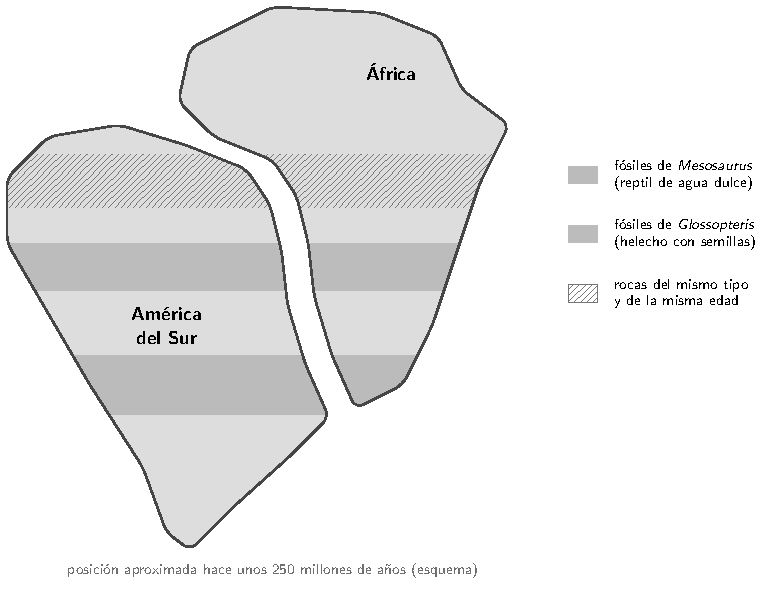
\includegraphics[max width=0.92\linewidth,max height=8.5cm]{fis/tie_wegener}
\end{center}
\subsection{Las evidencias de Wegener}
\textbf{1. Encaje de los continentes.} Las costas de América del Sur y de África calzan como piezas de un rompecabezas, y el ajuste es aún mejor si se usa el borde de la plataforma continental, bajo el mar.

 

\textbf{2. Fósiles.} Se encuentran fósiles de las mismas especies en continentes hoy separados por océanos. \emph{Mesosaurus}, un pequeño reptil de agua dulce, aparece solo en el sur de Brasil y en el sur de África: no pudo cruzar un océano salado. \emph{Glossopteris}, un helecho con semillas pesadas, aparece en América del Sur, África, India, Australia y la Antártica.

  

\textbf{3. Rocas y cordilleras.} Rocas del mismo tipo y la misma edad, y cordilleras con la misma estructura, continúan de un continente a otro: los montes Apalaches de América del Norte continúan en las montañas de Escocia y Escandinavia.

 

\textbf{4. Paleoclimas.} Hay huellas de antiguos glaciares en zonas que hoy son tropicales (India, África, Brasil) y restos de grandes bosques, convertidos en carbón, en la Antártica. Esos continentes estuvieron en otras latitudes.

 
\begin{clave}[{Recuerda}] Ninguna evidencia sola prueba la deriva; la fuerza del argumento está en que \textbf{evidencias independientes} apuntan a la misma conclusión: los continentes estuvieron unidos y se han desplazado.\end{clave}
\subsection{La expansión del fondo oceánico}
En la década de 1960, el estudio del fondo de los océanos dio la pieza que faltaba. \textbf{Harry Hess} propuso la \textbf{expansión del fondo oceánico}:

 
\begin{itemize}
  \item En las \textbf{dorsales oceánicas}, cordilleras submarinas como la dorsal mesoatlántica, sube \textbf{magma} desde el manto, se enfría y forma corteza oceánica nueva.
  \item La corteza nueva empuja a la anterior hacia ambos lados: el océano se ensancha unos pocos centímetros por año.
  \item En las \textbf{fosas oceánicas}, la corteza oceánica antigua se hunde en el manto (subducción). Así la Tierra no crece.
\end{itemize}
 

\textbf{Evidencias:} las rocas son más jóvenes junto a la dorsal y más antiguas a medida que se alejan, en forma simétrica; los sedimentos son más gruesos lejos de la dorsal; y la corteza oceánica más antigua tiene unos 180 millones de años, mucho menos que muchas rocas continentales.

  
\begin{center}
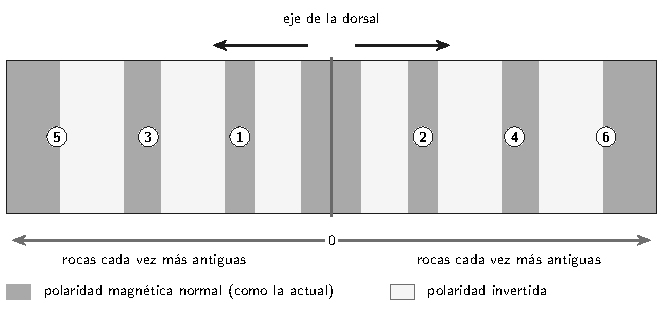
\includegraphics[max width=0.92\linewidth,max height=8.5cm]{fis/tie_dorsal}
\end{center}
 
\begin{clave}[{Bandas magnéticas}] Al solidificarse, algunos minerales de la roca quedan orientados según el campo magnético terrestre de ese momento, que se invierte cada cierto tiempo. Por eso el fondo muestra franjas de polaridad normal e invertida \textbf{simétricas} a ambos lados de la dorsal.\end{clave}
\subsection{Tectónica de placas y tipos de límites}
La \textbf{teoría de la tectónica de placas} une la deriva continental y la expansión del fondo oceánico. La capa externa rígida de la Tierra, la \textbf{litosfera}, está dividida en \textbf{placas} que se desplazan lentamente sobre la \textbf{astenosfera}, una capa plástica del manto. Los continentes no se mueven solos: viajan sobre las placas. La mayor actividad geológica ocurre en los \textbf{límites} entre placas.

 
\begin{center}
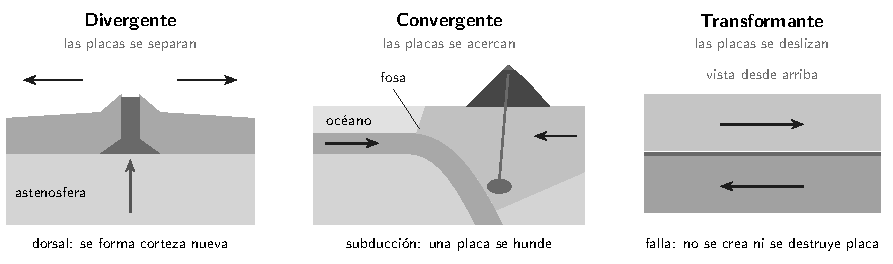
\includegraphics[max width=0.92\linewidth,max height=8.5cm]{fis/tie_limites}
\end{center}
 
\begin{center}\small
\begin{tabularx}{\linewidth}{@{}>{\raggedright\arraybackslash\hsize=0.97\hsize}X>{\raggedright\arraybackslash\hsize=1.10\hsize}X>{\raggedright\arraybackslash\hsize=1.10\hsize}X>{\raggedright\arraybackslash\hsize=0.83\hsize}X@{}}
\toprule
\textbf{Límite} & \textbf{Movimiento} & \textbf{Qué se forma} & \textbf{Ejemplo} \\
\midrule
Divergente & las placas se separan & dorsales, rift, corteza nueva, volcanismo, sismos poco profundos & dorsal mesoatlántica, Islandia \\
Convergente oceánica-continental & se acercan; la oceánica, más densa, se hunde (subducción) & fosa, cordillera, volcanes, sismos de todas las profundidades & Nazca bajo la Sudamericana \\
Convergente continental-continental & se acercan; ninguna se hunde mucho & grandes cordilleras por plegamiento & Himalaya \\
Transformante & se deslizan lateralmente & fallas, sismos; no se crea ni se destruye placa & falla de San Andrés \\
\bottomrule
\end{tabularx}
\end{center}
\subsection{Consecuencias: sismos, volcanismo y relieve en Chile}
Chile está sobre un límite \textbf{convergente}: la \textbf{placa de Nazca}, oceánica, se hunde bajo la \textbf{placa Sudamericana}, continental, a unos 6 a 7 cm por año. De esa subducción resultan:

 
\begin{itemize}
  \item \textbf{Fosa de Chile-Perú:} depresión submarina profunda donde la placa de Nazca empieza a hundirse.
  \item \textbf{Sismos:} las placas se traban en su contacto, acumulan energía y la liberan de golpe. Los hipocentros son más profundos hacia el este, siguiendo la placa que se hunde. Ahí ocurrió el mayor sismo registrado, Valdivia 1960 (magnitud 9,5).
  \item \textbf{Volcanismo:} a unos 100 km de profundidad, la placa que se hunde libera agua que hace fundir parcialmente el manto: se forma magma que asciende y alimenta los volcanes de los Andes.
  \item \textbf{Relieve:} la compresión levanta la cordillera de la Costa y la cordillera de los Andes.
\end{itemize}
  
\begin{center}
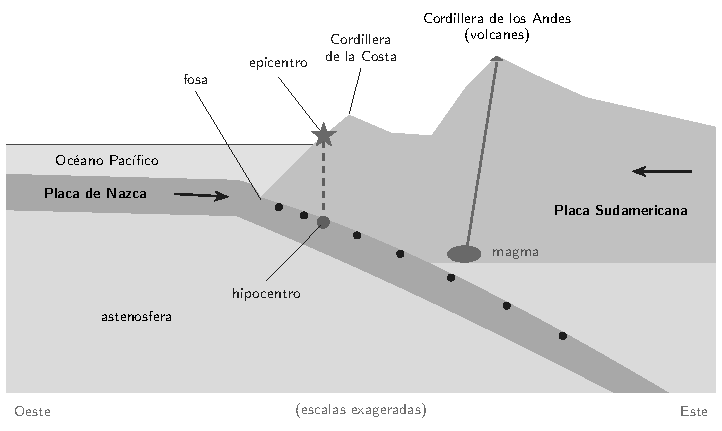
\includegraphics[max width=0.92\linewidth,max height=8.5cm]{fis/tie_chile}
\end{center}
 
\begin{clave}[{Recuerda}] En el extremo sur de Chile el contacto con la placa de Scotia es transformante: las placas se deslizan, hay sismos, pero no se formó una cordillera como los Andes.\end{clave}
\subsection{Lo clave del tema}
\begin{center}\small
\begin{tabularx}{\linewidth}{@{}>{\raggedright\arraybackslash\hsize=0.91\hsize}X>{\raggedright\arraybackslash\hsize=1.04\hsize}X>{\raggedright\arraybackslash\hsize=1.04\hsize}X@{}}
\toprule
\textbf{Idea} & \textbf{Qué dice} & \textbf{Evidencia o ejemplo} \\
\midrule
Deriva continental (Wegener) & los continentes estuvieron unidos en Pangea y se desplazaron & encaje, fósiles, rocas, paleoclimas \\
Expansión del fondo oceánico (Hess) & en las dorsales se forma corteza nueva; en las fosas se destruye & rocas más jóvenes junto a la dorsal, bandas magnéticas simétricas \\
Tectónica de placas & la litosfera está dividida en placas que se mueven sobre la astenosfera & sismos y volcanes concentrados en los bordes de placa \\
Límite divergente & placas se separan & dorsal mesoatlántica \\
Límite convergente & placas se acercan; subducción o colisión & Andes, Himalaya \\
Límite transformante & placas se deslizan lateralmente & San Andrés, Scotia-Sudamericana \\
\bottomrule
\end{tabularx}
\end{center}
 
\begin{clave}[{Recuerda}] · Wegener tenía evidencias, pero no un mecanismo; la tectónica de placas lo aportó.\par · Rocas a igual distancia de la dorsal tienen igual edad; más lejos, más antiguas.\par · Los Andes se formaron por la convergencia de las placas de Nazca y Sudamericana.\end{clave}
 
\begin{clave}[{Método PAES}] 1. Identifica el tipo de límite por el movimiento (se separan, se acercan, se deslizan). 2. Asocia sus consecuencias (dorsal, fosa y cordillera, falla). 3. En preguntas de investigación, busca qué medición responde directamente la pregunta y en qué escala de tiempo (las placas se mueven centímetros por año). 4. Descarta alternativas que no se deducen de los datos.\end{clave}
\begin{elejemplo}{PAES Regular 2026, adaptada}
Un equipo extrae rocas del fondo oceánico a ambos lados de una dorsal. Una roca obtenida a 50 km al oeste del eje de la dorsal tiene 2 millones de años.

Si la expansión del fondo oceánico ha sido constante e igual hacia ambos lados, ¿qué edad se espera para una roca extraída a 100 km al \textbf{este} del eje de la dorsal?
\alts{2 millones de años}{4 millones de años}{1 millón de años}{8 millones de años}
\solucion{\textbf{Paso 1. ¿Qué nos piden?} La edad de una roca del fondo oceánico según su distancia a la dorsal.

\textbf{Paso 2. Recuerda el proceso.} En la dorsal se forma roca nueva que se desplaza hacia ambos lados. Si la expansión es constante y simétrica, la edad de una roca es proporcional a su distancia al eje, sin importar de qué lado esté.

\textbf{Paso 3. Calcula.} A 50 km la roca tiene 2 millones de años. A 100 km, el doble de distancia, la roca tiene el doble de edad: 4 millones de años. De paso, la rapidez de expansión es $\dfrac{50 \text{ km}}{2 \text{ millones de años}}$, es decir, 2,5 cm por año.

\textbf{Respuesta:} 4 millones de años.

\textbf{¿Por qué no las otras?} 2 millones de años correspondería a una roca a 50 km del eje, hacia cualquiera de los lados. 1 millón de años invierte la relación: más lejos significa más antigua, no más joven. 8 millones de años supone que la edad crece con el cuadrado de la distancia.

\textbf{\color{cienciaD}Para recordar.} En una dorsal, la edad de la roca crece con la distancia al eje, igual hacia ambos lados.}{B}
\end{elejemplo}

%% =====================================================================
%% fis_interior
\section[Interior de la Tierra y sismos]{Interior de la Tierra y sismos}
\modcomun\ \ {\color{gris}\itshape Los modelos estático (corteza, manto y núcleo) y dinámico (litosfera, astenosfera, mesosfera y núcleo externo e interno) de la geosfera, las ondas sísmicas P y S, hipocentro y epicentro, magnitud e intensidad de un sismo y la energía que libera.\par}
\subsection{Dos modelos de la geosfera}
El interior de la Tierra se describe con dos modelos que se complementan:

 

\textbf{Modelo estático} (según la \textbf{composición química}):

 
\begin{itemize}
  \item \textbf{Corteza:} continental (5 a 70 km de espesor, rocas como el granito) u oceánica (5 a 10 km, basalto).
  \item \textbf{Manto:} hasta unos 2900 km; rocas de silicatos de hierro y magnesio.
  \item \textbf{Núcleo:} hasta el centro, a 6371 km; principalmente hierro y níquel.
\end{itemize}
 

\textbf{Modelo dinámico} (según el \textbf{comportamiento físico}: rígido, plástico o líquido):

 
\begin{itemize}
  \item \textbf{Litosfera:} rígida; corteza más la parte superior del manto, unos 100 km. Está dividida en placas.
  \item \textbf{Astenosfera:} parte del manto superior que se comporta como un material \textbf{plástico}: es sólida, pero fluye muy lentamente.
  \item \textbf{Mesosfera:} manto inferior, sólido, hasta los 2900 km.
  \item \textbf{Núcleo externo:} \textbf{líquido}, hasta unos 5150 km. Sus movimientos generan el campo magnético terrestre.
  \item \textbf{Núcleo interno:} \textbf{sólido}, por la enorme presión, aunque su temperatura supera los 5000 °C.
\end{itemize}
  
\begin{center}
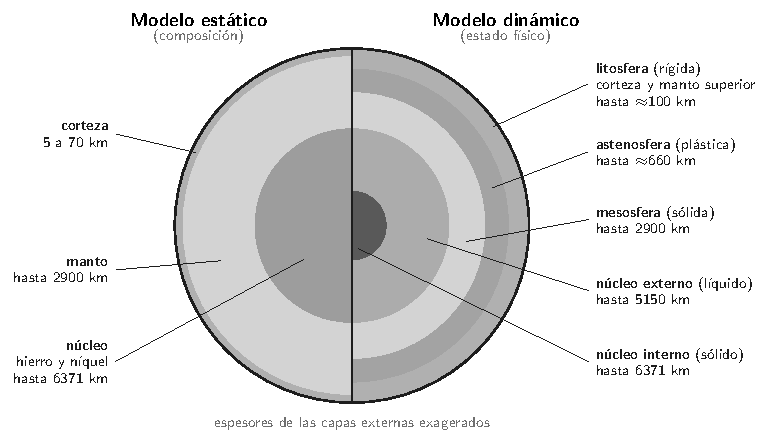
\includegraphics[max width=0.92\linewidth,max height=8.5cm]{fis/tie_capas}
\end{center}
 
\begin{clave}[{Recuerda}] La litosfera no es lo mismo que la corteza: incluye la corteza y una parte del manto. Y la astenosfera no es un océano de roca fundida: es roca sólida que se deforma lentamente.\end{clave}
\subsection{¿Cómo conocemos el interior? Las ondas sísmicas}
La perforación más profunda llega a unos 12 km. Todo lo demás se sabe estudiando cómo viajan las \textbf{ondas sísmicas}: su rapidez cambia según el material, y en los límites entre capas se reflejan y se refractan (cambian de dirección).

 
\begin{itemize}
  \item \textbf{Ondas P} (primarias): \textbf{longitudinales}, de compresión. Son las \textbf{más rápidas} (unos 6 km/s en la corteza) y viajan por sólidos, líquidos y gases.
  \item \textbf{Ondas S} (secundarias): \textbf{transversales}. Son más lentas (unos 3,5 km/s en la corteza) y \textbf{solo viajan por sólidos}.
  \item \textbf{Ondas superficiales:} viajan por la superficie, son las más lentas y las que más daño causan.
\end{itemize}
  
\begin{center}
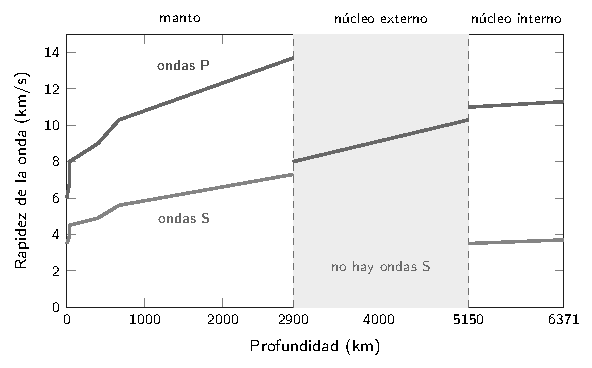
\includegraphics[max width=0.92\linewidth,max height=8.5cm]{fis/tie_velocidades}
\end{center}
 
\begin{clave}[{La gran pista}] A los 2900 km las ondas S \textbf{dejan de propagarse} y las ondas P se frenan bruscamente. Como las ondas S no viajan por líquidos, el \textbf{núcleo externo es líquido}. Por eso, en el lado opuesto de la Tierra al sismo existe una zona de sombra donde no llegan ondas S directas.\end{clave}
\subsection{Los sismos: hipocentro, epicentro y energía}
En los bordes de placa, las rocas quedan \textbf{trabadas} por el roce. Mientras las placas siguen moviéndose, las rocas se deforman y acumulan \textbf{energía elástica}, como un resorte que se comprime. Cuando la tensión supera la resistencia de la roca, esta se rompe y se desliza de golpe: la energía acumulada se libera como \textbf{ondas sísmicas}, calor y deformación del terreno. Eso es un \textbf{sismo}.

 
\begin{itemize}
  \item \textbf{Hipocentro} (o foco): punto en el interior de la Tierra donde se inicia la ruptura.
  \item \textbf{Epicentro:} punto de la \textbf{superficie} ubicado justo encima del hipocentro.
\end{itemize}
 

Si el epicentro está en el mar y el sismo levanta bruscamente el fondo oceánico, puede generar un \textbf{tsunami}.

  
\begin{center}
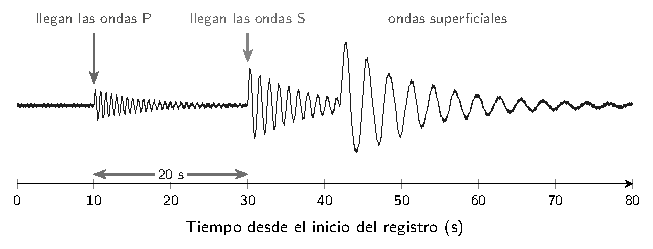
\includegraphics[max width=0.92\linewidth,max height=8.5cm]{fis/tie_sismograma}
\end{center}
 
\begin{clave}[{Distancia al sismo}] Las ondas P llegan primero porque son más rápidas. Mientras más lejos está la estación, mayor es el tiempo entre la llegada de las P y la de las S. Con ese intervalo se calcula la distancia al hipocentro, y con tres estaciones se ubica el epicentro.\end{clave}
\subsection{Magnitud e intensidad}
\textbf{Magnitud:} mide la \textbf{energía liberada} en el hipocentro. Cada sismo tiene \textbf{una sola magnitud}, que se calcula con los registros de los sismógrafos. Se usan la escala de Richter y, para sismos grandes, la escala de magnitud de momento (Mw). Son escalas \textbf{logarítmicas}: un grado más de magnitud significa unas \textbf{32 veces más energía}, y dos grados, unas 1000 veces más.

 

\textbf{Intensidad:} mide los \textbf{efectos} del sismo en un lugar: cómo lo percibieron las personas y qué daños produjo. Se expresa con la \textbf{escala de Mercalli}, de I a XII en números romanos. Un mismo sismo tiene \textbf{distintas intensidades} en distintos lugares: depende de la distancia al epicentro, de la profundidad, del tipo de suelo y de la calidad de las construcciones.

  
\begin{center}\small
\begin{tabularx}{\linewidth}{@{}>{\raggedright\arraybackslash\hsize=0.65\hsize}X>{\raggedright\arraybackslash\hsize=1.13\hsize}X>{\raggedright\arraybackslash\hsize=1.22\hsize}X@{}}
\toprule
 & \textbf{Magnitud} & \textbf{Intensidad} \\
\midrule
Qué mide & energía liberada & efectos y daños en un lugar \\
Cuántos valores & uno por sismo & uno por cada lugar \\
Escala & Richter o Mw (logarítmica) & Mercalli (I a XII) \\
Cómo se obtiene & con sismógrafos & con observaciones de efectos \\
\bottomrule
\end{tabularx}
\end{center}
 
\begin{ejemplo}[{Ejemplos chilenos}] Valdivia, 1960: magnitud 9,5, el mayor sismo registrado. Maule, 2010: magnitud 8,8, con un tsunami que afectó la costa centro-sur.\end{ejemplo}
\subsection{Lo clave del tema}
\begin{center}\small
\begin{tabularx}{\linewidth}{@{}>{\raggedright\arraybackslash\hsize=0.65\hsize}X>{\raggedright\arraybackslash\hsize=1.18\hsize}X>{\raggedright\arraybackslash\hsize=1.18\hsize}X@{}}
\toprule
\textbf{Concepto} & \textbf{Qué es} & \textbf{Dato clave} \\
\midrule
Modelo estático & capas según composición & corteza, manto, núcleo \\
Modelo dinámico & capas según comportamiento físico & litosfera rígida, astenosfera plástica, núcleo externo líquido \\
Ondas P & longitudinales, las más rápidas & viajan por sólidos y líquidos \\
Ondas S & transversales, más lentas & solo por sólidos: no cruzan el núcleo externo \\
Hipocentro y epicentro & origen interior y punto de superficie encima & el epicentro está sobre el hipocentro \\
Magnitud & energía liberada & una por sismo; +1 grado \ensuremath{\approx} 32 veces más energía \\
Intensidad & efectos en un lugar & Mercalli; cambia de un lugar a otro \\
\bottomrule
\end{tabularx}
\end{center}
 
\begin{clave}[{Recuerda}] · Si las ondas S desaparecen, la capa es líquida.\par · La litosfera incluye la corteza y parte del manto.\par · Un sismo tiene una magnitud y muchas intensidades.\end{clave}
 
\begin{clave}[{Método PAES}] 1. Distingue si la pregunta es de composición (modelo estático) o de comportamiento físico (modelo dinámico). 2. En gráficos de ondas, busca dónde cambian o desaparecen. 3. Para magnitud o intensidad, pregúntate si se habla de energía o de efectos. 4. En preguntas de investigación, busca el dato que se relaciona directamente con lo que se quiere saber.\end{clave}
\begin{elejemplo}{Estilo PAES}
Una estación sismológica registra un sismo. Las ondas S llegan 20 segundos después que las ondas P, como muestra el sismograma. En la zona, las ondas P viajan a 6 km/s y las ondas S a 4 km/s.

¿A qué distancia aproximada de la estación se originó el sismo?
\begin{center}
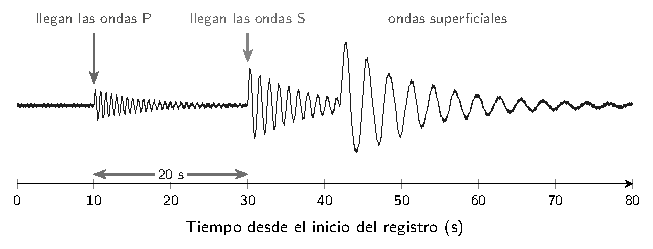
\includegraphics[max width=0.92\linewidth,max height=8.5cm]{fis/tie_sismograma}
\end{center}
\alts{120 km}{80 km}{200 km}{240 km}
\solucion{\textbf{Paso 1. ¿Qué nos piden?} La distancia $d$ al origen del sismo, a partir del retraso de las ondas S respecto de las P.

\textbf{Paso 2. Plantea los tiempos.} Ambas ondas recorren la misma distancia $d$ con rapidez constante, así que $t_P = \dfrac{d}{6}$ y $t_S = \dfrac{d}{4}$ (en segundos, con $d$ en km).

\textbf{Paso 3. Usa la diferencia.} $t_S - t_P = \dfrac{d}{4} - \dfrac{d}{6} = \dfrac{3d - 2d}{12} = \dfrac{d}{12}$. Como la diferencia es 20 s: $\dfrac{d}{12} = 20$, entonces $d = 240$ km.

\textbf{Comprobación:} $t_P = 240/6 = 40$ s y $t_S = 240/4 = 60$ s; la diferencia es 20 s. \ding{52}

\textbf{Respuesta:} 240 km.

\textbf{¿Por qué no las otras?} 120 km resulta de multiplicar 20 s por la rapidez de las ondas P, como si las P hubieran tardado 20 s en llegar. 80 km hace lo mismo con la rapidez de las S. 200 km resulta de multiplicar 20 s por la suma de las rapideces, que no tiene sentido físico.

\textbf{\color{cienciaD}Para recordar.} El retraso de las ondas S respecto de las P crece con la distancia: d/vS \ensuremath{-} d/vP = \ensuremath{\Delta}t.}{D}
\end{elejemplo}

\chapter{Electricidad}
%% =====================================================================
%% fis_corriente_ohm
\section[Corriente eléctrica y ley de Ohm]{Corriente eléctrica y ley de Ohm}
\modcomun\ \ {\color{gris}\itshape Qué es la corriente eléctrica y cómo se calcula (I = q/t), su sentido convencional, el voltaje y la resistencia, la ley de Ohm (V = I·R), la lectura de gráficos V--I (la pendiente es la resistencia), conductores óhmicos y no óhmicos, y cómo se conectan el amperímetro y el voltímetro.\par}
\subsection{La corriente eléctrica}
La materia está formada por partículas con \textbf{carga eléctrica}: protones (positivos) y electrones (negativos). La carga se mide en \textbf{coulomb} (C). En los metales, algunos electrones se pueden mover con libertad por el material.

 

La \textbf{corriente eléctrica} es un flujo ordenado de cargas a través de un conductor. Su \textbf{intensidad} $I$ indica cuánta carga $q$ atraviesa una sección del conductor en cada unidad de tiempo:

 \[ I = \dfrac{q}{t} \] 

Se mide en \textbf{ampere} (A): 1 A = 1 C/s. Si por un cable pasan 6 C en 3 s, la intensidad es $I = 6/3 = 2$ A.

 

Para que circule corriente se necesita un \textbf{circuito cerrado}: un camino conductor continuo que sale de la fuente (pila, batería, enchufe) y vuelve a ella. Si el circuito se abre en algún punto (un interruptor apagado, un cable cortado), la corriente se detiene en todo ese camino.

  
\begin{clave}[{Sentido de la corriente}] En un cable metálico, los electrones se mueven por el circuito externo desde el polo negativo hacia el polo positivo de la pila. Por una convención histórica, el \textbf{sentido convencional} de la corriente es el contrario: sale del polo \textbf{positivo}, recorre el circuito y vuelve por el polo \textbf{negativo}. Las flechas de corriente de los diagramas usan el sentido convencional.\end{clave}
 
\begin{clave}[{Recuerda}] · La corriente no se «gasta» al pasar por una ampolleta: la misma carga que entra por un extremo sale por el otro. Lo que la ampolleta transforma es \textbf{energía}.\par · Las pilas y baterías entregan \textbf{corriente continua} (siempre en el mismo sentido). La red domiciliaria entrega \textbf{corriente alterna}, que en Chile cambia de sentido 50 veces por segundo.\end{clave}
\subsection{Voltaje y resistencia}
La \textbf{diferencia de potencial} o \textbf{voltaje} $V$ es la energía que la fuente entrega a cada unidad de carga que pasa por ella. Se mide en \textbf{volt} (V): 1 V = 1 J/C. Una pila de 1,5 V entrega 1,5 J a cada coulomb; la red domiciliaria chilena tiene 220 V.

 

El voltaje es lo que impulsa a las cargas. Una analogía útil es el agua: la diferencia de altura entre dos estanques hace que el agua fluya por un tubo; el voltaje hace que la carga fluya por el cable.

 

La \textbf{resistencia eléctrica} $R$ mide cuánto se opone un elemento al paso de la corriente. Se mide en \textbf{ohm} (\ensuremath{\Omega}). Al atravesar una resistencia, la energía eléctrica se transforma en calor (efecto Joule), y en el filamento de una ampolleta también en luz.

  
\begin{clave}[{De qué depende la resistencia de un cable}] · Del \textbf{material}: el cobre conduce muy bien; el nicrom, que se usa en estufas, mucho peor.\par · Del \textbf{largo}: a mayor largo, mayor resistencia.\par · Del \textbf{área de la sección} (el grosor): a mayor grosor, menor resistencia.\par · De la \textbf{temperatura}: en los metales, la resistencia aumenta al calentarse.\end{clave}
 

En la analogía del agua, un tubo largo y delgado deja pasar menos agua por segundo que uno corto y ancho, con la misma diferencia de altura.

 
\begin{clave}[{Recuerda}] Los conductores (metales, grafito, agua con sales disueltas) tienen resistencia baja. Los aislantes (plástico, goma, vidrio, aire seco) tienen resistencia muy alta.\end{clave}
\subsection{Ley de Ohm}
En muchos conductores, si la temperatura se mantiene, la corriente es \textbf{directamente proporcional} al voltaje aplicado. Es la \textbf{ley de Ohm}:

 \[ V = I\cdot R \] 

Despejando se obtiene $I = \dfrac{V}{R}$ y $R = \dfrac{V}{I}$.

 

\textbf{Ejemplo 1.} Un hervidor tiene una resistencia de 22 \ensuremath{\Omega} y se conecta a 220 V: $I = 220/22 = 10$ A.

 

\textbf{Ejemplo 2.} Por un resistor circulan 0,5 A cuando se le aplican 6 V: $R = 6/0{,}5 = 12$ \ensuremath{\Omega}.

  
\begin{clave}[{Cómo leer la ley}] · Con la misma resistencia, si el voltaje se duplica, la corriente se duplica.\par · Con el mismo voltaje, si la resistencia se duplica, la corriente se reduce a la mitad.\par · Para aumentar la corriente: aumenta el voltaje o disminuye la resistencia.\end{clave}
 
\begin{clave}[{Recuerda}] Usa las unidades base: $V$ en volt, $I$ en ampere y $R$ en ohm. Si te dan miliampere, conviértelos: 200 mA = 0,2 A. Si te dan kiloohm: 2 k\ensuremath{\Omega} = 2000 \ensuremath{\Omega}.\end{clave}
\subsection{Gráficos V--I: conductores óhmicos y no óhmicos}
Si se mide la corriente para distintos voltajes y se grafica $V$ en función de $I$, un \textbf{conductor óhmico} da una \textbf{recta que pasa por el origen}. Su \textbf{pendiente es la resistencia}:

 \[ R = \dfrac{\Delta V}{\Delta I} \] 

En el gráfico, la recta azul pasa por (1 A; 10 V): su resistencia es 10 \ensuremath{\Omega}, la misma en cualquier punto.

 

Un \textbf{conductor no óhmico} no da una recta: su resistencia cambia con el voltaje. El filamento de una ampolleta se calienta cuando aumenta la corriente, y su resistencia aumenta: con 0,5 A tiene $3{,}5/0{,}5 = 7$ \ensuremath{\Omega}, y con 1 A tiene $10/1 = 10$ \ensuremath{\Omega}. Los diodos y los LED también son no óhmicos.

  
\begin{center}
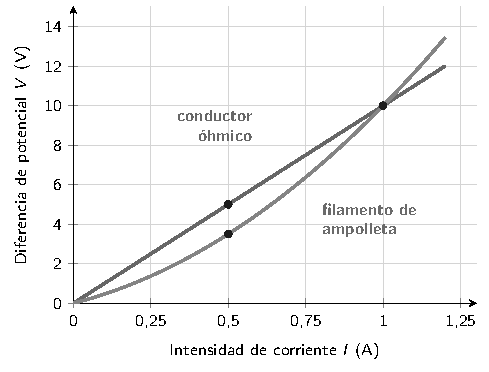
\includegraphics[max width=0.92\linewidth,max height=8.5cm]{fis/ele_vi_curva}
\end{center}
 
\begin{clave}[{Fíjate en los ejes}] Si el gráfico es de $I$ en función de $V$ (la corriente en el eje vertical), la pendiente es $\dfrac{1}{R}$: la resistencia es el \textbf{inverso de la pendiente}. En ese gráfico, la recta más inclinada es la de \textbf{menor} resistencia.\end{clave}
\subsection{Cómo medir corriente y voltaje}
El \textbf{amperímetro} mide la intensidad de corriente. Se conecta \textbf{en serie}: se abre el circuito y se intercala el instrumento, para que toda la corriente pase a través de él. Un buen amperímetro tiene una resistencia muy pequeña, para no alterar la corriente que mide.

 

El \textbf{voltímetro} mide la diferencia de potencial entre dos puntos. Se conecta \textbf{en paralelo} con el elemento, tocando sus dos extremos. Un buen voltímetro tiene una resistencia muy grande, para que casi no pase corriente por él.

 

El \textbf{óhmetro} mide resistencias, con el elemento desconectado del circuito. El \textbf{multímetro} (o tester) reúne los tres instrumentos.

  
\begin{center}
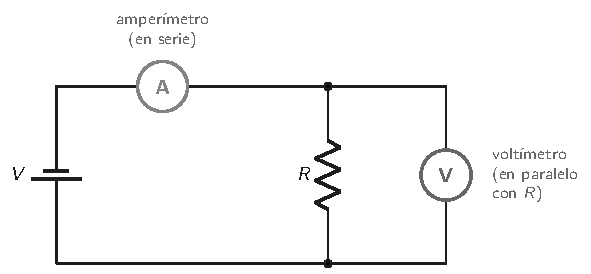
\includegraphics[max width=0.92\linewidth,max height=8.5cm]{fis/ele_medicion}
\end{center}
 
\begin{clave}[{Recuerda}] · Amperímetro: en serie, dentro del camino de la corriente.\par · Voltímetro: en paralelo, entre los extremos del elemento.\par · Para obtener una resistencia de forma experimental, mide $V$ con el voltímetro, mide $I$ con el amperímetro y calcula $R = V/I$.\end{clave}
\subsection{Lo clave del tema}
\begin{center}\small
\begin{tabularx}{\linewidth}{@{}>{\raggedright\arraybackslash\hsize=1.10\hsize}X>{\raggedright\arraybackslash\hsize=0.48\hsize}X>{\raggedright\arraybackslash\hsize=0.52\hsize}X>{\raggedright\arraybackslash\hsize=1.90\hsize}X@{}}
\toprule
\textbf{Magnitud} & \textbf{Símbolo} & \textbf{Unidad} & \textbf{Idea clave} \\
\midrule
Carga eléctrica & $q$ & coulomb (C) & propiedad de protones y electrones \\
Intensidad de corriente & $I$ & ampere (A) & $I = q/t$; se mide con amperímetro en serie \\
Voltaje & $V$ & volt (V) & energía por unidad de carga; se mide con voltímetro en paralelo \\
Resistencia & $R$ & ohm (\ensuremath{\Omega}) & aumenta con el largo y la temperatura; disminuye con el grosor \\
Ley de Ohm & \multicolumn{2}{@{}l@{}}{$V = I\cdot R$} & con $R$ constante, $I$ es proporcional a $V$ \\
Gráfico V--I óhmico & \multicolumn{2}{@{}l@{}}{recta por el origen} & pendiente de $V$ vs $I$ = $R$; pendiente de $I$ vs $V$ = $1/R$ \\
\bottomrule
\end{tabularx}
\end{center}
 
\begin{clave}[{Recuerda}] · La corriente no se gasta: lo que se transforma es la energía.\par · El sentido convencional va del polo positivo al negativo por el circuito externo; los electrones van al revés.\par · Un conductor no óhmico (filamento, LED) da una curva: su resistencia cambia.\end{clave}
 
\begin{clave}[{Método PAES}] 1. Anota los datos con sus unidades y conviértelas (mA a A, minutos a segundos). 2. Elige la fórmula: $I = q/t$ o $V = I\cdot R$. 3. En un gráfico, mira qué va en cada eje antes de usar la pendiente. 4. Revisa si el resultado tiene sentido: más voltaje, más corriente; más resistencia, menos corriente.\end{clave}
\begin{elejemplo}{PAES Invierno 2027, adaptada}
Un grupo de estudiantes conecta, por separado, dos resistencias óhmicas a una fuente de voltaje variable y mide la intensidad de corriente para distintos voltajes. Con los datos construye el gráfico de la figura.

Si se aplica una diferencia de potencial de 12 V a la resistencia 2, ¿qué intensidad de corriente circula por ella?
\begin{center}
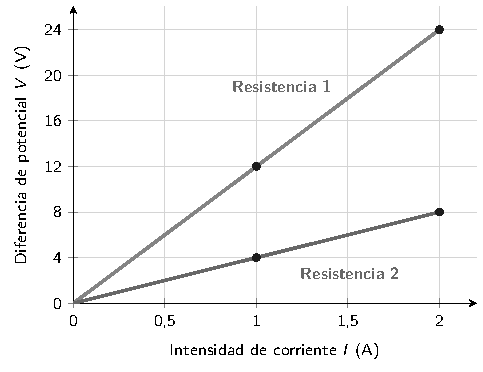
\includegraphics[max width=0.92\linewidth,max height=8.5cm]{fis/ele_vi}
\end{center}
\alts{1 A}{3 A}{48 A}{0,33 A}
\solucion{\textbf{Paso 1. ¿Qué nos piden?} La corriente en la resistencia 2 cuando se le aplican 12 V.

\textbf{Paso 2. Obtén la resistencia con la pendiente.} En un gráfico de $V$ en función de $I$, la pendiente es la resistencia. La recta 2 pasa por (2 A; 8 V): $R_2 = \dfrac{8}{2} = 4$ \ensuremath{\Omega}.

\textbf{Paso 3. Aplica la ley de Ohm.} La resistencia es óhmica (su gráfico es una recta por el origen), así que mantiene sus 4 \ensuremath{\Omega} aunque el voltaje sea mayor que los medidos: $I = \dfrac{V}{R} = \dfrac{12}{4} = 3$ A.

\textbf{Respuesta:} 3 A.

\textbf{¿Por qué no las otras?} 1 A es el resultado de usar la resistencia 1 (12 \ensuremath{\Omega}) en lugar de la 2. 48 A sale de multiplicar el voltaje por la resistencia, en vez de dividir. 0,33 A sale de dividir la resistencia por el voltaje.

\textbf{\color{cienciaD}Para recordar.} En un gráfico V--I, la pendiente es la resistencia; con ella, la ley de Ohm da la corriente.}{B}
\end{elejemplo}

%% =====================================================================
%% fis_circuitos
\section[Circuitos en serie, paralelo y mixtos]{Circuitos en serie, paralelo y mixtos}
\modcomun\ \ {\color{gris}\itshape Cómo se reparten la corriente y el voltaje en circuitos en serie y en paralelo, la resistencia equivalente, qué pasa al desconectar o fundir una ampolleta, el brillo relativo de ampolletas iguales, la ley de nudos y la resolución de circuitos mixtos.\par}
\subsection{Circuito en serie}
En un circuito \textbf{en serie} los elementos están uno a continuación del otro: la corriente tiene \textbf{un solo camino}.

 
\begin{itemize}
  \item \textbf{Corriente:} es la \textbf{misma} en todos los elementos.
  \item \textbf{Voltaje:} el de la fuente se \textbf{reparte} entre los elementos: $V = V_1 + V_2 + \dots$ El de mayor resistencia recibe más voltaje, porque $V_i = I\cdot R_i$.
  \item \textbf{Resistencia equivalente:} las resistencias se suman: $R_{\text{eq}} = R_1 + R_2 + \dots$ Siempre es mayor que la mayor de ellas.
\end{itemize}
 

\textbf{Ejemplo.} Resistencias de 2 \ensuremath{\Omega}, 4 \ensuremath{\Omega} y 6 \ensuremath{\Omega} en serie con una batería de 24 V: $R_{\text{eq}} = 12$ \ensuremath{\Omega} e $I = 24/12 = 2$ A. Los voltajes son $2\cdot 2 = 4$ V, $2\cdot 4 = 8$ V y $2\cdot 6 = 12$ V, que suman 24 V.

  
\begin{center}
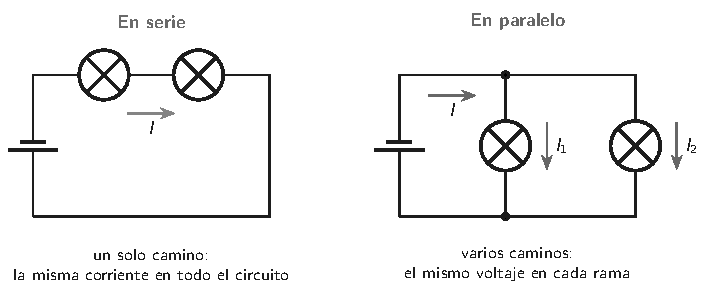
\includegraphics[max width=0.92\linewidth,max height=8.5cm]{fis/ele_serie_paralelo}
\end{center}
 
\begin{clave}[{Recuerda}] Si una ampolleta en serie se funde o se desconecta, el circuito se abre y \textbf{todas se apagan}. Al agregar más elementos en serie, la resistencia total aumenta y la corriente disminuye.\end{clave}
\subsection{Circuito en paralelo}
En un circuito \textbf{en paralelo} cada elemento se conecta directamente a los dos extremos de la fuente: la corriente tiene \textbf{varios caminos}, llamados ramas.

 
\begin{itemize}
  \item \textbf{Voltaje:} es el \textbf{mismo} en todas las ramas e igual al de la fuente.
  \item \textbf{Corriente:} la total se \textbf{reparte} entre las ramas: $I = I_1 + I_2 + \dots$ Por la rama de menor resistencia pasa más corriente.
  \item \textbf{Resistencia equivalente:} $\dfrac{1}{R_{\text{eq}}} = \dfrac{1}{R_1} + \dfrac{1}{R_2} + \dots$ Siempre es menor que la menor de ellas.
\end{itemize}
 

\textbf{Ejemplo.} Resistencias de 6 \ensuremath{\Omega} y 3 \ensuremath{\Omega} en paralelo con 12 V: $I_1 = 12/6 = 2$ A e $I_2 = 12/3 = 4$ A, así que $I = 6$ A y $R_{\text{eq}} = 12/6 = 2$ \ensuremath{\Omega}. Con la fórmula: $\dfrac{1}{R_{\text{eq}}} = \dfrac{1}{6} + \dfrac{1}{3} = \dfrac{3}{6}$, de donde $R_{\text{eq}} = 2$ \ensuremath{\Omega}.

  
\gatotip[\gatonegro]{\textbf{Atajos.} · Dos resistencias: $R_{\text{eq}} = \dfrac{R_1\cdot R_2}{R_1 + R_2}$.\par · $n$ resistencias iguales de valor $R$: $R_{\text{eq}} = \dfrac{R}{n}$.}
 
\begin{clave}[{Recuerda}] Si una rama se desconecta, las demás siguen funcionando igual (mismo voltaje, misma corriente), pero la corriente total que entrega la fuente disminuye. Al agregar ramas, la resistencia total disminuye y la corriente total aumenta. Por eso la instalación de una casa es en paralelo: cada artefacto funciona de forma independiente.\end{clave}
\subsection{Brillo de las ampolletas}
El brillo de una ampolleta depende de la \textbf{potencia} que disipa: $P = V\cdot I = I^2\cdot R = \dfrac{V^2}{R}$. Si las ampolletas son \textbf{iguales}, brilla más la que tiene \textbf{más corriente} (y, por lo tanto, más voltaje).

 

\textbf{En serie.} Dos ampolletas iguales en serie reciben la mitad del voltaje cada una: brillan menos que una sola conectada a la misma pila.

 

\textbf{En paralelo.} Cada ampolleta recibe el voltaje completo y brilla igual que si estuviera sola. A cambio, la pila entrega más corriente y se descarga antes.

 

\textbf{Circuito de la figura} (tres ampolletas iguales). Toda la corriente pasa por $L_1$ y luego se divide en partes iguales entre $L_2$ y $L_3$. Por eso $L_1$ brilla más, y $L_2$ y $L_3$ brillan igual entre sí.

  
\begin{center}
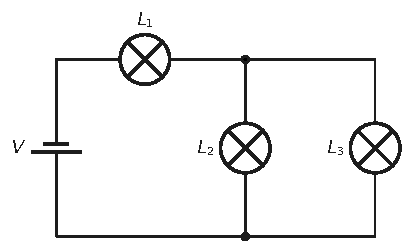
\includegraphics[max width=0.92\linewidth,max height=8.5cm]{fis/ele_brillo}
\end{center}
 
\begin{clave}[{Si se funde L3}] La resistencia total pasa de $R + \dfrac{R}{2} = 1{,}5R$ a $2R$: la corriente total disminuye y $L_1$ brilla menos. Toda esa corriente pasa ahora por $L_2$: antes recibía $\dfrac{V}{3R}$ y ahora recibe $\dfrac{V}{2R}$, así que $L_2$ brilla más.\end{clave}
\subsection{Circuitos mixtos}
Un circuito \textbf{mixto} combina partes en serie y partes en paralelo. Se resuelve por etapas, reemplazando grupos de resistencias por su equivalente:

 
\begin{enumerate}
  \item Reemplaza cada grupo en paralelo por su resistencia equivalente.
  \item Suma las resistencias que quedan en serie: obtienes $R_{\text{eq}}$.
  \item Calcula la corriente total: $I = V/R_{\text{eq}}$.
  \item Vuelve atrás: calcula el voltaje de cada parte y la corriente de cada rama.
\end{enumerate}
 

\textbf{En la figura.} $R_2$ y $R_3$ están en paralelo: $\dfrac{6\cdot 3}{6 + 3} = 2$ \ensuremath{\Omega}. En serie con $R_1$: $R_{\text{eq}} = 2 + 2 = 4$ \ensuremath{\Omega}. Corriente total: $I = 12/4 = 3$ A, que pasa entera por $R_1$. Voltaje en $R_1$: $3\cdot 2 = 6$ V, así que al paralelo le quedan 6 V. Corrientes: $6/6 = 1$ A por $R_2$ y $6/3 = 2$ A por $R_3$.

  
\begin{center}
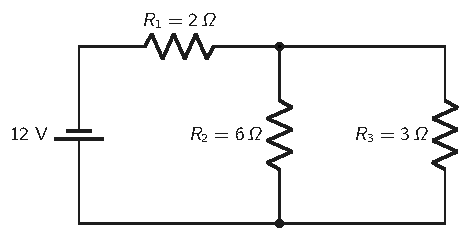
\includegraphics[max width=0.92\linewidth,max height=8.5cm]{fis/ele_mixto}
\end{center}
 
\begin{clave}[{Comprueba siempre}] Los voltajes de los tramos en serie suman el de la fuente (6 V + 6 V = 12 V), y las corrientes de las ramas suman la corriente total (1 A + 2 A = 3 A).\end{clave}
\subsection{Ley de nudos y lectura de datos}
Un \textbf{nudo} es un punto donde se unen tres o más cables. Como la carga no se crea ni se destruye, la corriente que \textbf{entra} a un nudo es igual a la que \textbf{sale} de él:

 \[ \sum I_{\text{entran}} = \sum I_{\text{salen}} \] 

Si a un nudo llegan 3 A y salen por dos ramas, y por una de ellas pasan 1,2 A, por la otra pasan $3 - 1{,}2 = 1{,}8$ A.

 

La corriente que entrega la batería es la suma de las corrientes de las ramas que salen del nudo conectado a ella.

  
\begin{clave}[{Inferir el tipo de conexión desde los datos}] · Si dos elementos tienen siempre la \textbf{misma corriente} y voltajes distintos, están en \textbf{serie}.\par · Si tienen siempre el \textbf{mismo voltaje} y corrientes distintas, están en \textbf{paralelo}.\par · En serie, el de mayor resistencia tiene más voltaje. En paralelo, el de mayor resistencia tiene menos corriente.\end{clave}
 
\begin{clave}[{Recuerda}] En serie se reparte el voltaje y la corriente es la misma. En paralelo se reparte la corriente y el voltaje es el mismo.\end{clave}
\subsection{Lo clave del tema}
\begin{center}\small
\begin{tabularx}{\linewidth}{@{}>{\raggedright\arraybackslash\hsize=0.82\hsize}X>{\raggedright\arraybackslash\hsize=0.99\hsize}X>{\raggedright\arraybackslash\hsize=1.19\hsize}X@{}}
\toprule
 & \textbf{En serie} & \textbf{En paralelo} \\
\midrule
Caminos para la corriente & uno solo & uno por rama \\
Corriente & la misma en todos & se reparte: $I = I_1 + I_2 + \dots$ \\
Voltaje & se reparte: $V = V_1 + V_2 + \dots$ & el mismo en todas las ramas \\
Resistencia equivalente & $R_1 + R_2 + \dots$ (mayor que cada una) & $\dfrac{1}{R_{\text{eq}}} = \dfrac{1}{R_1} + \dfrac{1}{R_2} + \dots$ (menor que cada una) \\
Al agregar un elemento & $R_{\text{eq}}$ aumenta, $I$ disminuye & $R_{\text{eq}}$ disminuye, $I$ total aumenta \\
Si un elemento se funde & se apagan todos & los demás siguen igual \\
\bottomrule
\end{tabularx}
\end{center}
 
\begin{clave}[{Recuerda}] · Con ampolletas iguales, brilla más la que lleva más corriente.\par · En un nudo, la corriente que entra es igual a la que sale.\par · En un circuito mixto, reduce primero los grupos en paralelo.\end{clave}
 
\begin{clave}[{Método PAES}] 1. Identifica qué elementos están en serie (mismo camino) y cuáles en paralelo (mismos dos nudos). 2. Calcula la resistencia equivalente por etapas. 3. Obtén la corriente total con $I = V/R_{\text{eq}}$. 4. Vuelve atrás para repartir voltajes y corrientes. 5. Comprueba: voltajes en serie suman el total; corrientes de las ramas suman la total.\end{clave}
\begin{elejemplo}{Estilo PAES}
En el circuito de la figura, la batería entrega una diferencia de potencial de 12 V.

¿Cuál es la intensidad de corriente que circula por la resistencia $R_3$?
\begin{center}
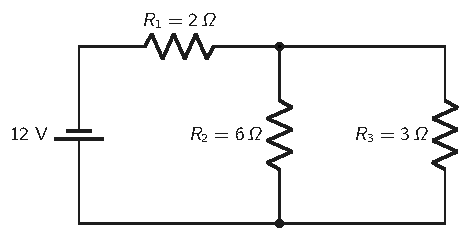
\includegraphics[max width=0.92\linewidth,max height=8.5cm]{fis/ele_mixto}
\end{center}
\alts{3 A}{1 A}{4 A}{2 A}
\solucion{\textbf{Paso 1. ¿Qué nos piden?} La corriente en una de las ramas del paralelo.

\textbf{Paso 2. Reduce el paralelo.} $R_2$ y $R_3$ en paralelo: $\dfrac{6\cdot 3}{6 + 3} = 2$ \ensuremath{\Omega}.

\textbf{Paso 3. Resistencia equivalente y corriente total.} En serie con $R_1$: $R_{\text{eq}} = 2 + 2 = 4$ \ensuremath{\Omega}. $I = \dfrac{12}{4} = 3$ A.

\textbf{Paso 4. Voltaje del paralelo.} En $R_1$ caen $3\cdot 2 = 6$ V; quedan $12 - 6 = 6$ V para $R_2$ y $R_3$.

\textbf{Paso 5. Corriente en $R_3$.} $I_3 = \dfrac{6}{3} = 2$ A. Comprobación: por $R_2$ pasa $6/6 = 1$ A, y $1 + 2 = 3$ A, la corriente total.

\textbf{Respuesta:} 2 A.

\textbf{¿Por qué no las otras?} 3 A es la corriente total, que se divide entre las dos ramas. 1 A es la corriente de $R_2$. 4 A sale de aplicar los 12 V completos a $R_3$, olvidando que una parte del voltaje queda en $R_1$.

\textbf{\color{cienciaD}Para recordar.} En un circuito mixto: reduce, calcula la corriente total y vuelve atrás para repartir.}{D}
\end{elejemplo}

%% =====================================================================
%% fis_potencia
\section[Potencia, energía y consumo eléctrico]{Potencia, energía y consumo eléctrico}
\modcomun\ \ {\color{gris}\itshape Potencia eléctrica (P = V·I = I²·R = V²/R), energía consumida en joule y en kWh, cálculo del costo de la cuenta de la luz y los componentes de la instalación eléctrica de una casa: medidor, tablero, diferencial, conexión a tierra y enchufes en paralelo.\par}
\subsection{Potencia eléctrica}
La \textbf{potencia eléctrica} $P$ es la energía que un artefacto transforma en cada segundo. Se mide en \textbf{watt} (W): 1 W = 1 J/s.

 \[ P = V\cdot I \] 

Combinándola con la ley de Ohm se obtienen otras dos formas, útiles según los datos que tengas:

 \[ P = I^2\cdot R \qquad P = \dfrac{V^2}{R} \] 

\textbf{Ejemplo.} Un hervidor de 2200 W conectado a 220 V: $I = \dfrac{P}{V} = \dfrac{2200}{220} = 10$ A, y $R = \dfrac{V}{I} = \dfrac{220}{10} = 22$ \ensuremath{\Omega}. Comprobación: $I^2 R = 100\cdot 22 = 2200$ W.

  
\begin{clave}[{Qué dice la etiqueta}] Una ampolleta que indica «60 W, 220 V» transforma 60 J de energía eléctrica en cada segundo cuando se conecta a 220 V.\end{clave}
 
\begin{clave}[{Recuerda}] · Con el mismo voltaje (en paralelo, como en una casa): \textbf{menor resistencia, mayor potencia} ($P = V^2/R$). Por eso un hervidor tiene mucha menos resistencia que una ampolleta.\par · Con la misma corriente (en serie): \textbf{mayor resistencia, mayor potencia} ($P = I^2R$).\par · La potencia total de un circuito es la suma de las potencias de sus elementos, estén en serie o en paralelo.\end{clave}
\subsection{Energía eléctrica y kilowatt hora}
La \textbf{energía} que consume un artefacto depende de su potencia y del tiempo que funciona:

 \[ E = P\cdot t \] 

Con $P$ en W y $t$ en s, la energía queda en joule (J). Para el consumo de una casa el joule es una unidad muy pequeña, y se usa el \textbf{kilowatt hora} (kWh): la energía que consume un artefacto de 1 kW funcionando durante 1 hora.

 \[ 1\ \text{kWh} = 1000\ \text{W}\cdot 3600\ \text{s} = 3.600.000\ \text{J} \] 

Para calcular en kWh, pasa la potencia a kW (divide por 1000) y el tiempo a horas.

  
\begin{ejemplo}[{Ejemplo: la cuenta de la luz}] Un microondas de 1200 W se usa 30 minutos al día durante 30 días. Energía: $E = 1{,}2\ \text{kW}\cdot 0{,}5\ \text{h}\cdot 30 = 18$ kWh. Si el kWh cuesta 200 pesos, el costo es $18\cdot 200 = 3600$ pesos. El medidor de la casa registra la energía total: la cuenta se calcula con la diferencia entre dos lecturas, multiplicada por el precio del kWh.\end{ejemplo}
 
\begin{clave}[{Recuerda}] La potencia indica qué tan rápido se consume la energía; el consumo y el costo dependen también del tiempo de uso. Un aparato de 10 W encendido todo el mes (720 h) consume 7,2 kWh, más que un secador de pelo de 1500 W usado 5 minutos al día durante 30 días (3,75 kWh).\end{clave}
\subsection{La instalación eléctrica de una casa}
\begin{center}
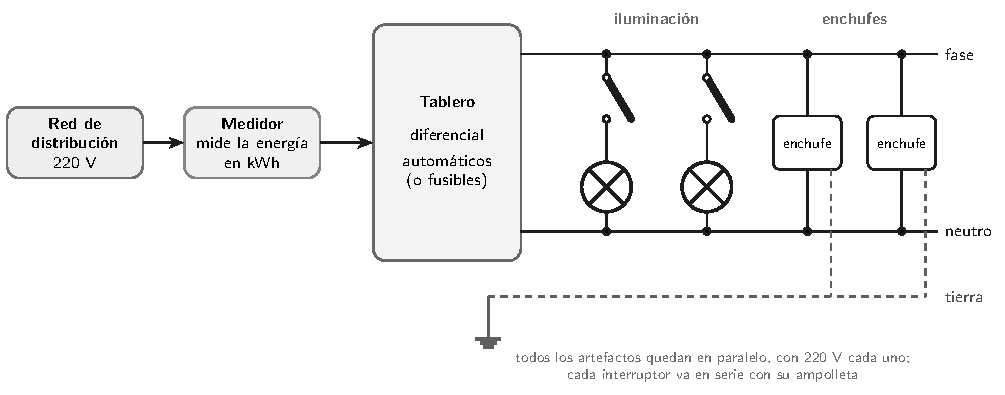
\includegraphics[max width=0.92\linewidth,max height=8.5cm]{fis/ele_instalacion}
\end{center}
  
\begin{itemize}
  \item \textbf{Medidor:} registra la energía consumida, en kWh. Con sus lecturas se calcula la cuenta.
  \item \textbf{Tablero:} reparte la energía en varios circuitos (iluminación, enchufes, cocina) y contiene las protecciones, como el diferencial.
\end{itemize}
  
\begin{itemize}
  \item \textbf{Diferencial:} detecta fugas de corriente a tierra (por ejemplo, a través de una persona que toca un artefacto dañado) y corta en milésimas de segundo. Protege a las personas.
  \item \textbf{Conexión a tierra:} el terminal central del enchufe une la carcasa metálica de los artefactos con la tierra, para que una fuga se descargue por ese cable y no a través de quien toca el artefacto.
  \item \textbf{Enchufes y ampolletas:} conectados \textbf{en paralelo}, todos reciben 220 V y funcionan de forma independiente. Cada interruptor va \textbf{en serie} con la ampolleta que controla.
\end{itemize}
 
\begin{clave}[{Recuerda}] Los aparatos que funcionan con un voltaje menor (celulares, notebooks) usan un cargador con un \textbf{transformador}, que reduce los 220 V de la red al voltaje que necesitan.\end{clave}
\subsection{Lo clave del tema}
\begin{center}\small
\begin{tabularx}{\linewidth}{@{}>{\raggedright\arraybackslash\hsize=0.74\hsize}X>{\raggedright\arraybackslash\hsize=1.64\hsize}X>{\raggedright\arraybackslash\hsize=0.62\hsize}X@{}}
\toprule
\textbf{Concepto} & \textbf{Fórmula o función} & \textbf{Unidad} \\
\midrule
Potencia eléctrica & $P = V\cdot I = I^2 R = V^2/R$ & watt (W) \\
Energía & $E = P\cdot t$ & joule (J) o kWh \\
Kilowatt hora & 1 kWh = 3.600.000 J & kWh \\
Costo & energía en kWh × precio del kWh & pesos \\
Medidor & registra la energía consumida & kWh \\
Diferencial & corta si detecta una fuga de corriente a tierra &  \\
Conexión a tierra & desvía las fugas de la carcasa a tierra &  \\
\bottomrule
\end{tabularx}
\end{center}
 
\begin{clave}[{Recuerda}] · En una casa todo está en paralelo a 220 V: más artefactos encendidos, más corriente total.\par · La potencia dice qué tan rápido se consume la energía; el costo depende también del tiempo.\par · El medidor registra la energía consumida, no la potencia.\end{clave}
 
\begin{clave}[{Método PAES}] 1. Identifica qué piden: potencia, energía, costo, corriente o un componente. 2. Pasa las unidades: W a kW y minutos a horas para kWh; segundos para joule. 3. Elige la forma de la potencia que use tus datos ($VI$, $I^2R$ o $V^2/R$). 4. En instalaciones, recuerda que todo está en paralelo a 220 V: cada artefacto suma su corriente a la total.\end{clave}
\begin{elejemplo}{Estilo PAES}
En una casa se usa un hervidor de 2000 W durante 15 minutos al día, todos los días de un mes de 30 días. El precio de la energía eléctrica es de 180 pesos por kWh.

¿Cuánto cuesta la energía que consume el hervidor en ese mes?
\alts{90 pesos}{2.700 pesos}{162.000 pesos}{2.700.000 pesos}
\solucion{\textbf{Paso 1. ¿Qué nos piden?} El costo mensual del consumo de un artefacto.

\textbf{Paso 2. Pasa a las unidades del kWh.} Potencia: 2000 W = 2 kW. Tiempo diario: 15 min = 0,25 h. Tiempo en el mes: $0{,}25\cdot 30 = 7{,}5$ h.

\textbf{Paso 3. Calcula la energía.} $E = P\cdot t = 2\cdot 7{,}5 = 15$ kWh.

\textbf{Paso 4. Calcula el costo.} $15\cdot 180 = 2700$ pesos.

\textbf{Respuesta:} 2.700 pesos.

\textbf{¿Por qué no las otras?} 90 pesos es el costo de un solo día (0,5 kWh): falta multiplicar por los 30 días. 162.000 pesos sale de usar 15 horas en vez de 15 minutos. 2.700.000 pesos sale de dejar la potencia en W en lugar de pasarla a kW.

\textbf{\color{cienciaD}Para recordar.} Costo = potencia en kW × horas de uso × precio del kWh.}{B}
\end{elejemplo}

\chapter{Habilidades científicas}
%% =====================================================================
%% fis_hab_investigacion
\section[Preguntas, hipótesis y variables]{Preguntas, hipótesis y variables}
\modcomun\ \ {\color{gris}\itshape Cómo se arma una investigación en física: pregunta investigable, hipótesis y predicción, variables independiente, dependiente y controladas, ensayo de referencia, instrumentos de medición, componentes de una investigación y un diseño experimental que cambie solo una variable.\par}
\subsection{La investigación científica paso a paso}
Buena parte de la PAES de Física no te pide una fórmula: te describe un experimento con péndulos, resortes, láseres o circuitos y te pregunta por su \textbf{pregunta}, su \textbf{hipótesis}, sus \textbf{variables} o su \textbf{conclusión}. Todas esas preguntas siguen el mismo esquema.

  

\textbf{Un ejemplo completo.}

 

\textbf{1. Observación.} Un columpio con cadenas largas va y viene más lento que uno con cadenas cortas.

 

\textbf{2. Pregunta.} ¿Cómo influye el largo de un péndulo en su período?

 

\textbf{3. Hipótesis.} El largo del péndulo influye en su período.

 

\textbf{4. Predicción.} Si la hipótesis es correcta, un péndulo de 100 cm tardará más en completar una oscilación que uno de 25 cm.

 

\textbf{5. Procedimiento.} Se cuelga la misma masa de hilos de 25, 50, 75 y 100 cm, se suelta siempre desde 10° y se mide con un cronómetro el tiempo de 10 oscilaciones, que luego se divide por 10.

 

\textbf{6. Resultados.} 1,0 s; 1,4 s; 1,7 s y 2,0 s.

 

\textbf{7. Conclusión.} En el rango estudiado, a mayor largo del péndulo, mayor es su período.

  
\begin{clave}[{Pregunta investigable}] Es una pregunta que se puede responder \textbf{midiendo} u observando algo. Casi siempre relaciona dos variables: «¿cómo influye A en B?».\end{clave}
 
\begin{clave}[{¿Investigable o no?}] · «¿Influye la tensión de una cuerda en la rapidez de las ondas que viajan por ella?»: sí, se cambia la tensión y se mide la rapidez.\par · «¿Es la luz azul más bonita que la roja?»: no, es una opinión.\par · «¿Qué día exacto ocurrirá el próximo gran sismo en Valparaíso?»: no se puede responder con mediciones hoy.\end{clave}
 
\begin{clave}[{Recuerda}] La pregunta de investigación calza con el procedimiento. Si un estudiante cierra un circuito y anota la corriente cada cinco minutos, la pregunta es «¿cómo cambia la intensidad de corriente con el tiempo de funcionamiento?», no una pregunta sobre el voltaje o el interruptor.\end{clave}
\subsection{Hipótesis y predicción}
La \textbf{hipótesis} es una respuesta tentativa a la pregunta. Tiene tres rasgos:

 
\begin{itemize}
  \item Se plantea \textbf{antes} del experimento.
  \item Relaciona la variable que se cambia con la que se mide: «la temperatura del agua influye en la refracción de la luz».
  \item Se puede poner a prueba, y podría resultar falsa.
\end{itemize}
 

La \textbf{predicción} es más concreta: dice qué resultado se espera en \textbf{este} experimento si la hipótesis es cierta. Suele tener la forma «si\dots{}, entonces\dots{}».

 
\begin{center}\small
\begin{tabularx}{\linewidth}{@{}>{\raggedright\arraybackslash\hsize=1.00\hsize}X>{\raggedright\arraybackslash\hsize=1.00\hsize}X@{}}
\toprule
\textbf{Hipótesis} & \textbf{Predicción} \\
\midrule
La tensión de una cuerda influye en la rapidez de las ondas que viajan por ella. & Si se cuelga el doble de masa del extremo de la cuerda, el pulso recorrerá los 2 m en menos tiempo. \\
La temperatura del agua influye en la refracción de la luz. & Al calentar el agua, el ángulo de refracción del láser cambiará. \\
El largo de un conductor influye en su resistencia eléctrica. & Una barra de grafito de 20 cm tendrá más resistencia que una de 10 cm del mismo grosor. \\
\bottomrule
\end{tabularx}
\end{center}
  
\begin{ejemplo}[{Ejemplo resuelto: ¿qué hipótesis se puso a prueba?}] Un cilindro con agua y un émbolo tiene tres orificios a distintas profundidades, cada uno conectado a un tubo en U. Los estudiantes anotan la altura del líquido en cada tubo, presionan el émbolo y vuelven a anotar: las tres alturas suben.\par \textbf{Paso 1.} ¿Qué cambia? La presión sobre la superficie del líquido (se presiona el émbolo).\par \textbf{Paso 2.} ¿Qué se mide? La altura en cada tubo, que indica la presión en cada punto del líquido.\par \textbf{Paso 3.} La hipótesis une ambas: «al aumentar la presión sobre la superficie de un líquido, aumenta la presión en todos sus puntos».\par Una hipótesis sobre la densidad del líquido o el área de los orificios no se pone a prueba aquí: esas variables no cambiaron.\end{ejemplo}
 
\begin{clave}[{Recuerda}] La hipótesis va antes de experimentar; la conclusión, después, apoyada en los datos. Un experimento no «demuestra» una hipótesis para siempre: la apoya o la contradice.\end{clave}
\subsection{Variables: independiente, dependiente y controladas}
\begin{center}
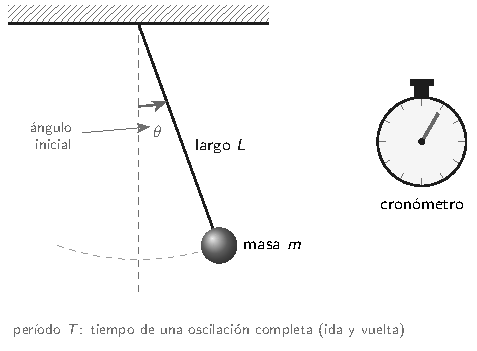
\includegraphics[max width=0.92\linewidth,max height=8.5cm]{fis/hab_pendulo}
\end{center}
  

En el péndulo del ejemplo se cambia el largo del hilo y se mide el período con un cronómetro.

 
\begin{center}\small
\begin{tabularx}{\linewidth}{@{}>{\raggedright\arraybackslash\hsize=0.50\hsize}X>{\raggedright\arraybackslash\hsize=1.25\hsize}X>{\raggedright\arraybackslash\hsize=1.25\hsize}X@{}}
\toprule
\textbf{Variable} & \textbf{Cómo reconocerla} & \textbf{En el péndulo} \\
\midrule
\textbf{Independiente} & La que el investigador \textbf{cambia a propósito} (la causa). & Largo del hilo \\
\textbf{Dependiente} & La que se \textbf{mide} como respuesta (el efecto). & Período de oscilación \\
\textbf{Controladas} & Las que se dejan \textbf{iguales} para que no influyan. & Masa, ángulo inicial, tipo de hilo, forma de medir el tiempo \\
\bottomrule
\end{tabularx}
\end{center}
 
\gatotip[\gatoatigrado]{\textbf{Truco de la frase.} Arma la frase «el efecto de \textbf{[independiente]} sobre \textbf{[dependiente]}». Aquí: «el efecto del largo sobre el período». Si la frase no tiene sentido, cambiaste el orden.}
  
\begin{ejemplo}[{Ejemplo resuelto}] Con una fuente de poder variable, un estudiante aplica 2, 4, 6 y 8 V a un mismo resistor y mide la corriente con un amperímetro. Todo a temperatura ambiente.\par · Cambia a propósito: la diferencia de potencial \ensuremath{\rightarrow} \textbf{independiente}.\par · Se mide al final: la intensidad de corriente \ensuremath{\rightarrow} \textbf{dependiente}.\par · Siempre igual: el resistor y la temperatura \ensuremath{\rightarrow} \textbf{controladas}.\end{ejemplo}
 
\begin{clave}[{Recuerda}] Si cambias la masa de un bloque, también cambian su peso y la fuerza normal que el piso ejerce sobre él: esas fuerzas no son variables controladas. Una variable controlada es algo que de verdad se mantiene igual en todos los ensayos, como la superficie, la compresión del resorte o el ángulo de lanzamiento.\end{clave}
\subsection{Ensayo de referencia, comparaciones justas e instrumentos}
El \textbf{grupo control} o \textbf{ensayo de referencia} es la medición sin el factor que se estudia. Para saber cuánto bloquea una caja metálica la señal de un celular, se mide la señal fuera de la caja (referencia) y dentro de ella. Sin la referencia no sabrías si la caja hizo algo.

 

\textbf{Compara solo ensayos que se diferencian en una cosa.}

 
\begin{center}\small
\begin{tabular}{@{}lll@{}}
\toprule
\textbf{Ensayo} & \textbf{Largo (cm)} & \textbf{Masa (g)} \\
\midrule
1 & 50 & 100 \\
2 & 100 & 100 \\
3 & 100 & 200 \\
\bottomrule
\end{tabular}
\end{center}
 

· 1 y 2: solo cambia el largo \ensuremath{\rightarrow} sirven para estudiar el largo.\par · 2 y 3: solo cambia la masa \ensuremath{\rightarrow} sirven para estudiar la masa.\par · 1 y 3: cambian dos cosas \ensuremath{\rightarrow} no permiten saber cuál causó la diferencia.

 
\begin{center}
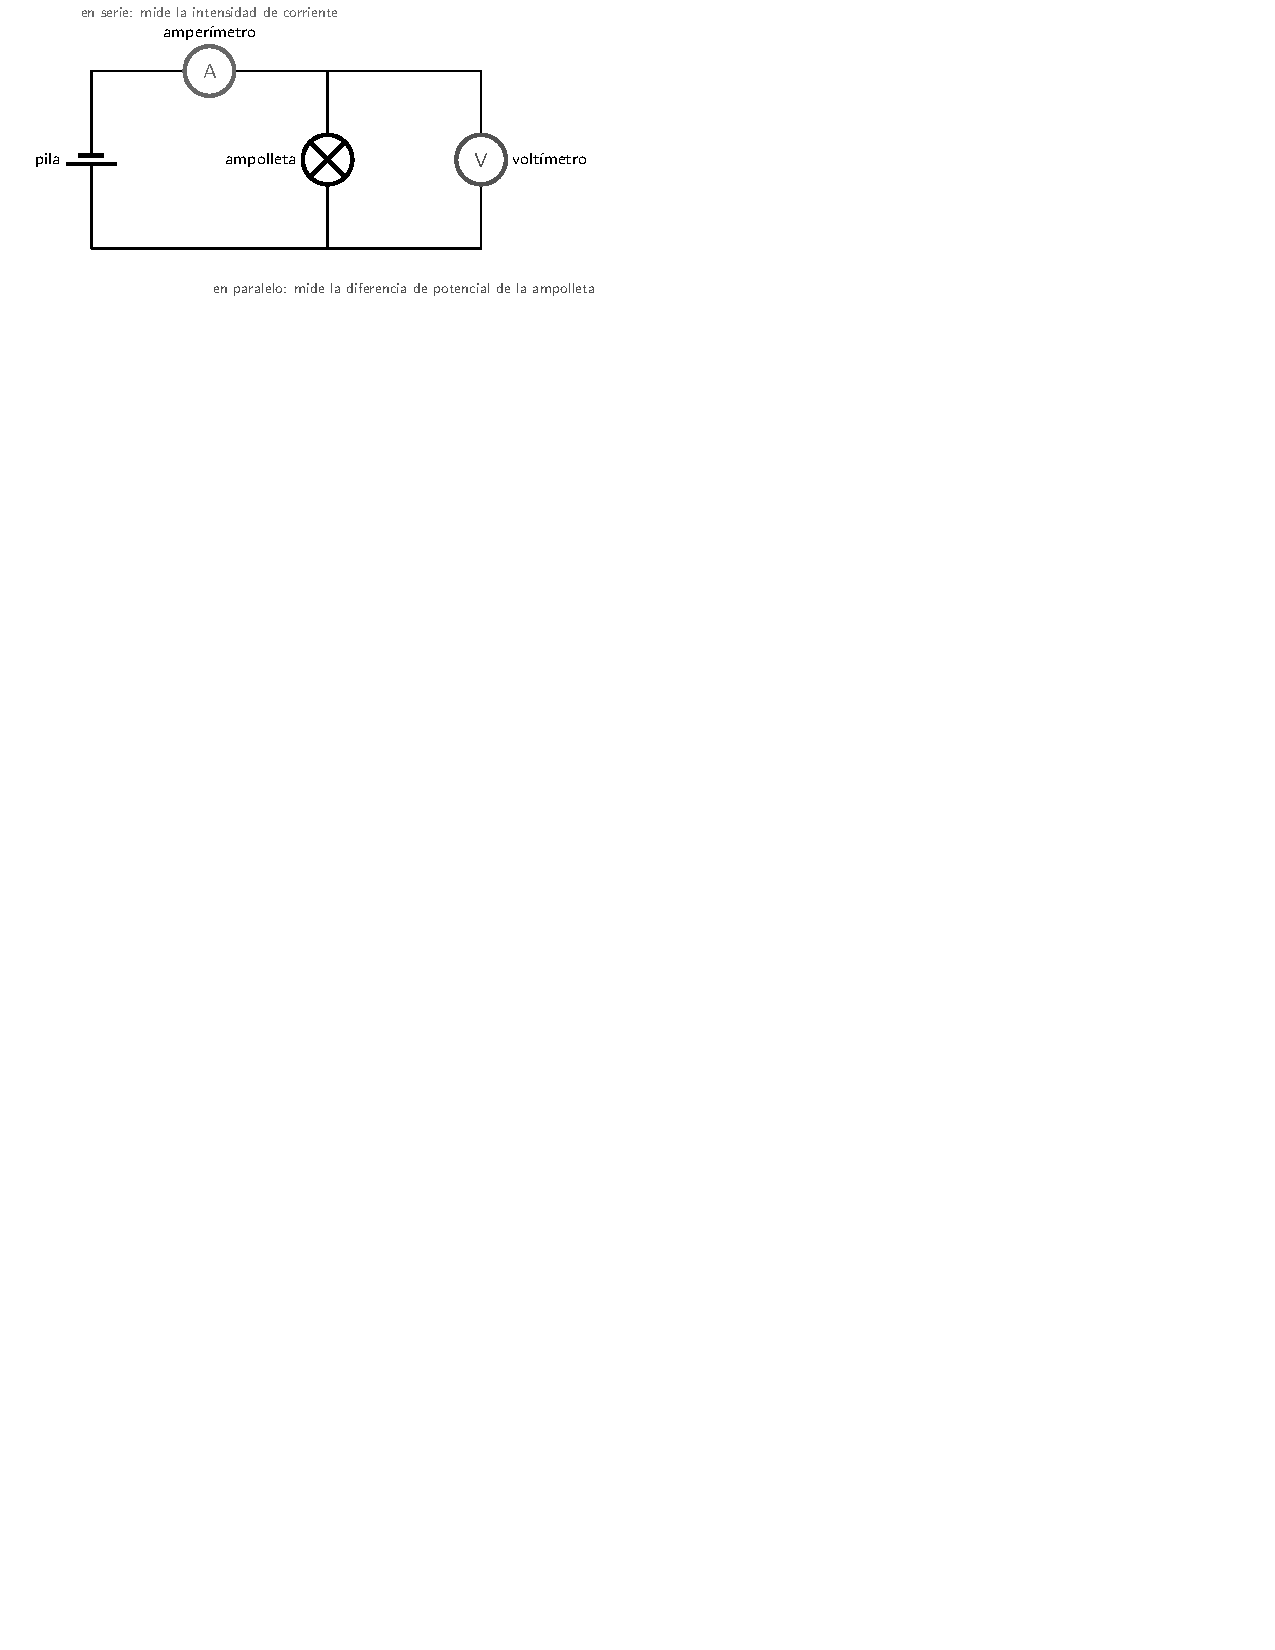
\includegraphics[max width=0.92\linewidth,max height=8.5cm]{fis/hab_circuito}
\end{center}
  
\begin{clave}[{Instrumentos según la variable}] \begin{center}\small
\begin{tabular}{@{}ll@{}}
\toprule
\textbf{Para medir\dots{}} & \textbf{se usa\dots{}} \\
\midrule
longitud, deformación de un resorte & regla o huincha \\
masa & balanza \\
fuerza (peso, tensión, roce) & dinamómetro \\
tiempo, período & cronómetro \\
ángulos (reflexión, refracción) & transportador \\
posición y rapidez de un móvil & sensor de movimiento \\
temperatura & termómetro \\
intensidad de corriente & amperímetro, en serie \\
diferencia de potencial & voltímetro, en paralelo \\
resistencia eléctrica & óhmetro (multímetro) \\
energía eléctrica consumida & medidor eléctrico (kWh) \\
vibraciones del suelo & sismógrafo \\
\bottomrule
\end{tabular}
\end{center}\end{clave}
 
\begin{clave}[{Recuerda}] Antes de elegir un instrumento, identifica qué variable piden. Si se estudia cómo la masa de un objeto influye en la fuerza necesaria para moverlo, la balanza mide la variable independiente y el dinamómetro, la dependiente.\end{clave}
\subsection{Los componentes de una investigación}
La PAES pregunta mucho «¿a qué componente de la investigación corresponde la frase entre comillas?». Apréndete esta tabla:

 
\begin{center}\small
\begin{tabularx}{\linewidth}{@{}>{\raggedright\arraybackslash\hsize=0.62\hsize}X>{\raggedright\arraybackslash\hsize=1.19\hsize}X>{\raggedright\arraybackslash\hsize=1.19\hsize}X@{}}
\toprule
\textbf{Componente} & \textbf{Qué es} & \textbf{Ejemplo en física} \\
\midrule
\textbf{Marco conceptual} & Lo que ya se sabe: leyes, teorías y modelos. & «Según la ley de Hooke, la deformación de un resorte es proporcional a la fuerza». \\
\textbf{Problema / pregunta} & Lo que se quiere averiguar. & «¿Cómo influye el ángulo de tiro en la aceleración de una maleta?». \\
\textbf{Objetivo} & Lo que se quiere lograr; empieza con un verbo en infinitivo. & «Determinar la relación entre el largo de una barra de grafito y su resistencia». \\
\textbf{Hipótesis} & Respuesta tentativa que se pone a prueba. & «La tensión de la cuerda influye en la rapidez de la onda». \\
\textbf{Predicción} & Resultado concreto esperado. & «Si suelto las dos esferas a la vez, llegarán juntas al suelo». \\
\textbf{Procedimiento} & Los pasos que se siguen. & «Se colgaron masas de 100 g y se midió el estiramiento con una regla». \\
\textbf{Observación} & Lo que se percibe directamente. & «Los paracaidistas no llegaron al suelo al mismo tiempo». \\
\textbf{Resultado / evidencia} & Los datos obtenidos. & «El ángulo de refracción del haz violeta fue 40,19°». \\
\textbf{Inferencia} & Interpretación que va más allá de lo observado. & «Los paracaídas deben tener tamaños distintos». \\
\textbf{Conclusión} & Respuesta a la pregunta, apoyada en los resultados. & «La fuerza de roce no depende del área de contacto». \\
\bottomrule
\end{tabularx}
\end{center}
  
\begin{clave}[{Pistas en el texto}] · «si\dots{}, entonces\dots{} ocurrirá»: predicción.\par · «determinar», «comparar», «evaluar», en infinitivo: objetivo.\par · «se colgó, se midió, se repitió»: procedimiento.\par · «se obtuvo», «los valores fueron»: resultado.\par · «debe ser», «esto sugiere», «podría indicar»: inferencia.\par · Responde la pregunta a partir de los datos: conclusión.\end{clave}
  
\begin{clave}[{Recuerda}] Observar es registrar lo que se ve («no todos llegan juntos»). Inferir es proponer algo que no se vio, a partir de lo observado y de lo que se sabe («entonces los paracaídas deben ser de distinto tamaño»). La conclusión, en cambio, sale de los resultados de una investigación diseñada para responder una pregunta.\end{clave}
\subsection{Diseñar un procedimiento y reconocer su objetivo}
Un buen procedimiento sigue cinco pasos:

 

\textbf{Paso 1.} Lee el objetivo y nombra la variable independiente (la que vas a cambiar) y la dependiente (la que vas a medir).

 

\textbf{Paso 2.} Elige varios valores de la independiente: 25, 50, 75 y 100 cm.

 

\textbf{Paso 3.} Deja \textbf{todo lo demás igual}: misma masa, mismo ángulo inicial, mismo hilo.

 

\textbf{Paso 4.} Decide con qué instrumento medirás la dependiente: cronómetro.

 

\textbf{Paso 5.} \textbf{Repite} cada medición y saca un promedio.

 
\begin{clave}[{Recuerda}] El objetivo de una investigación calza con lo que se varió y con lo que se midió. Si una persona tira de una maleta con la misma fuerza, cambia el ángulo y mide la aceleración, su objetivo es «determinar el efecto del ángulo sobre la aceleración», no sobre el peso ni sobre la magnitud de la fuerza.\end{clave}
  
\begin{ejemplo}[{Ejemplo resuelto: un modelo para estudiar un fenómeno}] Se quiere estudiar cómo el área de la sección transversal de un conductor afecta su capacidad de conducir corriente. Como la corriente se parece a un flujo de agua, se usan dos contenedores a distinta altura unidos por un tubo.\par \textbf{Paso 1.} ¿Qué representa cada parte? El tubo es el conductor; su \textbf{radio} representa el área de la sección; el caudal de agua representa la corriente.\par \textbf{Paso 2.} ¿Qué se varía? El radio del tubo.\par \textbf{Paso 3.} ¿Qué se mide? Qué tan rápido se llena el contenedor de abajo (el caudal).\par \textbf{Paso 4.} ¿Qué se deja igual? El largo del tubo, la diferencia de altura y el volumen inicial de agua.\par Variar el largo del tubo o la diferencia de altura estudiaría otras variables (el largo del conductor o el voltaje).\end{ejemplo}
\subsection{Lo clave del tema}
\begin{center}\small
\begin{tabularx}{\linewidth}{@{}>{\raggedright\arraybackslash\hsize=0.96\hsize}X>{\raggedright\arraybackslash\hsize=1.04\hsize}X@{}}
\toprule
\textbf{Concepto} & \textbf{Lo que tienes que reconocer} \\
\midrule
Pregunta de investigación & Se responde midiendo; calza con lo que se varió y lo que se midió. \\
Hipótesis & Respuesta tentativa que relaciona la variable independiente con la dependiente. \\
Predicción & Resultado concreto esperado: «si\dots{}, entonces\dots{}». \\
Variable independiente & La que se cambia a propósito. \\
Variable dependiente & La que se mide. \\
Variables controladas & Las que se mantienen iguales en todos los ensayos. \\
Ensayo de referencia & Medición sin el factor estudiado, para comparar. \\
Instrumento & El que mide la variable pedida: regla, balanza, dinamómetro, cronómetro, amperímetro, voltímetro\dots{} \\
Observación / inferencia / conclusión & Lo que se ve / lo que se deduce más allá / la respuesta a la pregunta con los datos. \\
\bottomrule
\end{tabularx}
\end{center}
 
\begin{clave}[{Recuerda}] · Para estudiar una variable, compara ensayos que solo difieren en esa variable.\par · Si cambias la masa, también cambian el peso y la normal: no son controladas.\par · La hipótesis habla de la variable que cambia en el experimento.\par · El amperímetro va en serie y el voltímetro en paralelo.\par · El instrumento que registra el resultado suele delatar la variable dependiente.\end{clave}
 
\begin{clave}[{Método PAES}] 1. Subraya qué se cambió, qué se midió y qué se dejó igual. 2. Con eso, nombra las tres variables. 3. Si preguntan por la hipótesis, la pregunta o el objetivo, elige la que relaciona exactamente esas dos variables. 4. Si preguntan por un componente, busca las pistas («si\dots{} entonces», «se obtuvo», «debe ser»). 5. Descarta las alternativas que hablan de variables que no cambiaron.\end{clave}
\begin{elejemplo}{Estilo PAES}
Un grupo de estudiantes investiga de qué depende el período de un péndulo. Arma cuatro péndulos como el de la figura y los suelta en las condiciones de la tabla:

\begin{center}\small
\begin{tabular}{@{}llll@{}}
\toprule
\textbf{Ensayo} & \textbf{Largo del hilo (cm)} & \textbf{Masa (g)} & \textbf{Ángulo inicial (°)} \\
\midrule
1 & 50 & 100 & 10 \\
2 & 100 & 100 & 10 \\
3 & 100 & 200 & 10 \\
4 & 50 & 200 & 20 \\
\bottomrule
\end{tabular}
\end{center}

¿Qué par de ensayos permite estudiar el efecto de la \textbf{masa} sobre el período?
\begin{center}
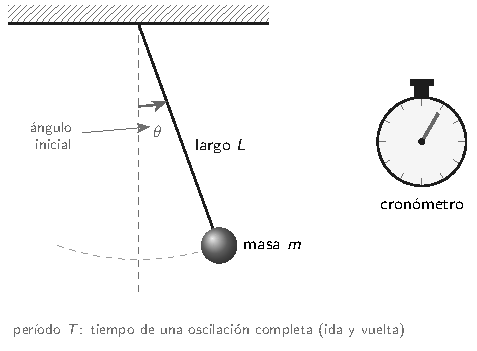
\includegraphics[max width=0.92\linewidth,max height=8.5cm]{fis/hab_pendulo}
\end{center}
\alts{Los ensayos 1 y 2.}{Los ensayos 2 y 3.}{Los ensayos 1 y 4.}{Los ensayos 3 y 4.}
\solucion{\textbf{Paso 1. ¿Qué nos piden?} Un par de ensayos que sirva para estudiar la masa. Dos ensayos sirven para estudiar una variable solo si se diferencian \textbf{únicamente} en esa variable; así, si el período cambia, sabemos qué lo causó.

\textbf{Paso 2. Ensayos 1 y 2.} Largo: 50 y 100 (cambia). Masa: 100 y 100 (igual). Ángulo: 10 y 10 (igual). Solo cambia el largo: este par sirve para estudiar el \textbf{largo}, no la masa.

\textbf{Paso 3. Ensayos 2 y 3.} Largo: 100 y 100 (igual). Masa: 100 y 200 (cambia). Ángulo: 10 y 10 (igual). Solo cambia la masa: este par sirve. \ding{52}

\textbf{Paso 4. Ensayos 1 y 4.} Largo igual, pero cambian la masa (100 y 200) y el ángulo (10 y 20). Con dos cambios a la vez no se puede atribuir la diferencia a la masa.

\textbf{Paso 5. Ensayos 3 y 4.} Masa igual (200), pero cambian el largo y el ángulo. No sirve.

\textbf{Respuesta:} los ensayos 2 y 3.

\textbf{Comprobación:} en los ensayos 2 y 3 la masa es la variable independiente; el largo (100 cm) y el ángulo (10°) son variables controladas. Si los estudiantes hacen el experimento, encontrarán que el período casi no cambia: para ángulos pequeños, el período de un péndulo no depende de la masa.

\textbf{¿Por qué no las otras?} En los ensayos 1 y 2 la masa es la misma: ese par estudia el largo. En los pares 1 y 4 y 3 y 4 cambian dos variables a la vez, así que cualquier diferencia en el período podría deberse a cualquiera de ellas.

\textbf{\color{cienciaD}Para recordar.} Para estudiar una variable, compara solo ensayos que se diferencian únicamente en esa variable.}{B}
\end{elejemplo}

%% =====================================================================
%% fis_hab_evidencia
\section[Procesar y analizar evidencia]{Procesar y analizar evidencia}
\modcomun\ \ {\color{gris}\itshape Leer tablas y gráficos de experimentos de física, reconocer tendencias y relaciones de proporcionalidad directa e inversa, interpretar la pendiente, interpolar y predecir con cuidado, hacer cálculos rápidos con los datos y elegir conclusiones que se apoyan en ellos.\par}
\subsection{Leer una tabla de datos}
Antes de mirar las alternativas, lee la tabla en este orden:

 

\textbf{1. Encabezados y unidades.} ¿Qué variable está en cada columna y en qué unidad?

 

\textbf{2. ¿Cuál se cambió?} Suele ser la primera columna, con valores «redondos» (0, 10, 20, 30).

 

\textbf{3. Tendencia.} Recorre la columna medida de arriba abajo: ¿sube, baja, se mantiene, sube y luego baja?

 

\textbf{4. Compara de a pares.} «Cuando la temperatura aumenta, la rapidez aumenta».

 
\begin{center}\small
\begin{tabular}{@{}ll@{}}
\toprule
\textbf{Temperatura del aire (°C)} & \textbf{Rapidez del sonido (m/s)} \\
\midrule
0 & 331 \\
10 & 337 \\
20 & 343 \\
30 & 349 \\
\bottomrule
\end{tabular}
\end{center}
  
\begin{ejemplo}[{Ejemplo resuelto}] En la tabla, ¿cómo se relacionan las variables?\par \textbf{Paso 1.} Tendencia: a mayor temperatura, mayor rapidez del sonido.\par \textbf{Paso 2.} Variación: cada 10 °C la rapidez aumenta 6 m/s. El aumento es constante: la relación es \textbf{lineal}.\par \textbf{Paso 3.} ¿Es proporcional? No: a 0 °C la rapidez no es cero (es 331 m/s), y al duplicar la temperatura de 10 a 20 °C la rapidez no se duplica.\par \textbf{Conclusión:} en el rango estudiado, la rapidez del sonido aumenta en forma lineal con la temperatura.\end{ejemplo}
 
\begin{clave}[{Recuerda}] Cuando una tabla tiene varias columnas medidas (altitud, presión, temperatura, densidad), cada afirmación de las alternativas relaciona solo dos. Revísalas de a una, leyendo bien el sentido: «disminuye cuando la altitud disminuye» es lo opuesto de «disminuye cuando la altitud aumenta».\end{clave}
\subsection{Leer un gráfico}
\begin{center}
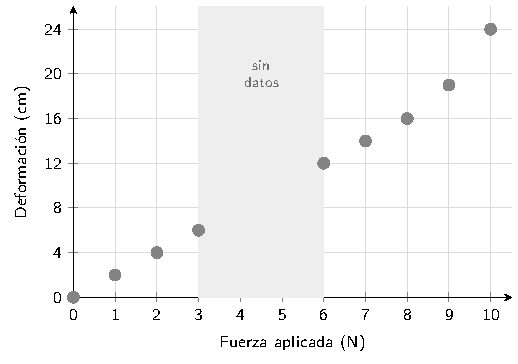
\includegraphics[max width=0.92\linewidth,max height=8.5cm]{fis/hab_hooke}
\end{center}
  

\textbf{1. Ejes.} ¿Qué variable va en cada eje y con qué unidad? Aquí: fuerza aplicada (N) en el eje horizontal, deformación del resorte (cm) en el vertical.

 

\textbf{2. Forma.} Entre 0 y 8 N los puntos están sobre una recta que pasa por el origen: la deformación es \textbf{proporcional} a la fuerza (ley de Hooke), 2 cm por cada newton.

 

\textbf{3. Zonas.} Con 9 y 10 N la deformación crece más rápido: el resorte \textbf{deja de cumplir la ley de Hooke}; se acerca o supera su límite elástico.

 

\textbf{4. Huecos.} Entre 3 y 6 N no hay mediciones. Se puede estimar con la tendencia de los puntos vecinos.

 
\begin{clave}[{Recuerda}] Un punto aislado no es una tendencia. Mira el conjunto de puntos y fíjate dónde cambia el comportamiento: ahí suele estar la respuesta.\end{clave}
\subsection{Relaciones entre variables}
\begin{center}
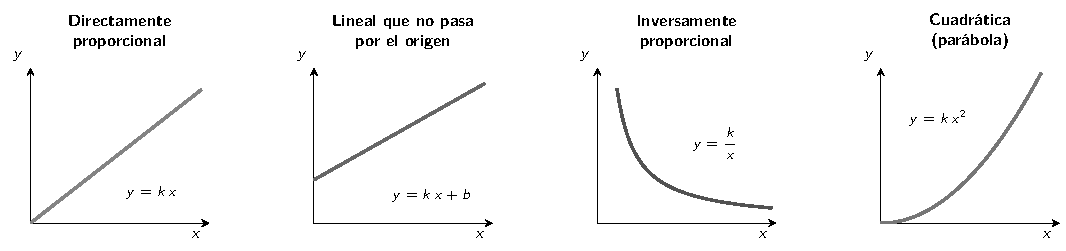
\includegraphics[max width=0.92\linewidth,max height=8.5cm]{fis/hab_relaciones}
\end{center}
  
\begin{center}\small
\begin{tabularx}{\linewidth}{@{}>{\raggedright\arraybackslash\hsize=0.71\hsize}X>{\raggedright\arraybackslash\hsize=1.14\hsize}X>{\raggedright\arraybackslash\hsize=1.14\hsize}X@{}}
\toprule
\textbf{Relación} & \textbf{Prueba con los datos} & \textbf{Ejemplo en física} \\
\midrule
\textbf{Directamente proporcional} & El \textbf{cociente} $y/x$ es constante. & Ley de Hooke: $F = k\,x$. Ley de Ohm: $V = I\,R$. \\
\textbf{Lineal, no proporcional} & Aumentos iguales, pero no pasa por el origen. & Largo total de un resorte: largo natural + deformación. \\
\textbf{Inversamente proporcional} & El \textbf{producto} $x\cdot y$ es constante. & Ondas en un mismo medio: $\lambda = \dfrac{v}{f}$. \\
\textbf{Cuadrática} & Al duplicar $x$, $y$ se cuadruplica. & Caída libre desde el reposo: $d = 5\,t^2$ (m, s). \\
\bottomrule
\end{tabularx}
\end{center}
  
\begin{ejemplo}[{Ejemplo resuelto}] Por una misma cuerda viajan ondas de 10, 20 y 40 Hz con longitudes de onda de 2,0; 1,0 y 0,5 m.\par \textbf{Paso 1.} Productos: $10\cdot 2{,}0 = 20$; $20\cdot 1{,}0 = 20$; $40\cdot 0{,}5 = 20$.\par \textbf{Paso 2.} El producto es constante: $\lambda$ y $f$ son \textbf{inversamente proporcionales}, y ese producto es la rapidez de la onda, 20 m/s.\end{ejemplo}
 
\begin{clave}[{Recuerda}] «Cuando una aumenta, la otra aumenta» no basta para decir que son proporcionales. Comprueba el cociente: si al duplicar una la otra no se duplica, la relación es otra. El período de un péndulo, por ejemplo, crece con el largo, pero para duplicar el período hay que \textbf{cuadruplicar} el largo.\end{clave}
\subsection{La pendiente en los gráficos de física}
En un gráfico con forma de recta, la \textbf{pendiente} es $\dfrac{\Delta y}{\Delta x}$, y en física casi siempre significa algo:

 
\begin{center}\small
\begin{tabularx}{\linewidth}{@{}>{\raggedright\arraybackslash\hsize=1.03\hsize}X>{\raggedright\arraybackslash\hsize=0.97\hsize}X@{}}
\toprule
\textbf{Gráfico (vertical vs. horizontal)} & \textbf{La pendiente es\dots{}} \\
\midrule
Fuerza vs. deformación & la constante elástica $k$ \\
Diferencia de potencial vs. corriente & la resistencia $R$ \\
Corriente vs. diferencia de potencial & el inverso de la resistencia, $1/R$ \\
Posición vs. tiempo & la velocidad \\
Velocidad vs. tiempo & la aceleración \\
\bottomrule
\end{tabularx}
\end{center}
 
\begin{clave}[{Recuerda}] Fíjate qué variable está en cada eje. Si el gráfico es de corriente en función del voltaje, la recta más empinada corresponde a la resistencia \textbf{menor}, porque deja pasar más corriente con el mismo voltaje.\end{clave}
  
\begin{center}
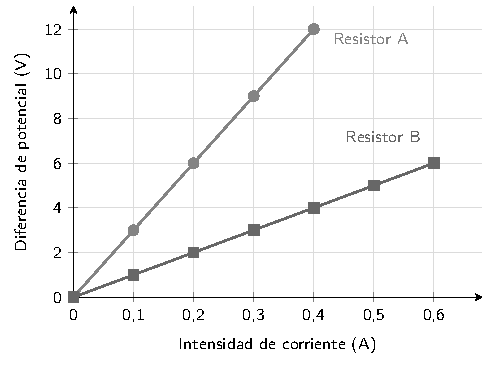
\includegraphics[max width=0.92\linewidth,max height=8.5cm]{fis/hab_ohm}
\end{center}
 
\begin{ejemplo}[{Ejemplo resuelto}] ¿Cuánto vale la resistencia B?\par \textbf{Paso 1.} El gráfico es de voltaje en función de la corriente: la pendiente es $R$.\par \textbf{Paso 2.} Toma un punto de la recta: 6 V con 0,6 A.\par \textbf{Paso 3.} $R = \dfrac{V}{I} = \dfrac{6}{0{,}6} = 10$ \ensuremath{\Omega}.\end{ejemplo}
\subsection{Tendencias: interpolar y predecir}
\textbf{Interpolar} es estimar un valor \textbf{dentro} del rango medido, siguiendo la tendencia. Es confiable si la tendencia es clara.

 

\textbf{Extrapolar} es estimar \textbf{fuera} del rango medido. Es riesgoso: el comportamiento puede cambiar, como el resorte que sobre 8 N deja de cumplir la ley de Hooke.

 
\begin{ejemplo}[{Ejemplo resuelto: interpolar}] Con la tabla de la rapidez del sonido (331 m/s a 0 °C; 337 a 10 °C; 343 a 20 °C; 349 a 30 °C), ¿qué rapidez se espera a 25 °C?\par \textbf{Paso 1.} 25 °C está entre 20 y 30 °C, dentro del rango.\par \textbf{Paso 2.} La rapidez sube 6 m/s cada 10 °C, es decir, 3 m/s cada 5 °C.\par \textbf{Paso 3.} $343 + 3 = 346$ m/s.\end{ejemplo}
  
\begin{ejemplo}[{Ejemplo resuelto: predecir con una relación}] Un péndulo de 1,0 m tiene un período de 2,0 s. ¿Qué largo necesita para un período de 4,0 s?\par \textbf{Paso 1.} El período crece con la raíz del largo: $T = 2\pi\sqrt{L/g}$.\par \textbf{Paso 2.} Para duplicar el período hay que multiplicar el largo por $2^2 = 4$.\par \textbf{Paso 3.} $L = 4{,}0$ m. Pensar «doble de período, doble de largo» daría 2,0 m, un error típico.\end{ejemplo}
 
\begin{clave}[{Recuerda}] Dentro del rango, sigue la tendencia de los puntos vecinos. Fuera del rango, desconfía de cualquier alternativa que afirme un valor exacto o un comportamiento que no se midió.\end{clave}
\subsection{De los datos a la conclusión}
Una conclusión correcta cumple cuatro condiciones:

 

\textbf{1.} Habla de las variables que se \textbf{midieron}.

 

\textbf{2.} Respeta el \textbf{sentido} de la tendencia («a mayor\dots{}, mayor\dots{}»).

 

\textbf{3.} No va más allá del \textbf{rango} estudiado.

 

\textbf{4.} No afirma \textbf{causas} ni mecanismos que los datos no muestran.

 
\begin{center}\small
\begin{tabular}{@{}ll@{}}
\toprule
\textbf{Tensión de la cuerda (N)} & \textbf{Rapidez del pulso (m/s)} \\
\midrule
4 & 10 \\
16 & 20 \\
36 & 30 \\
\bottomrule
\end{tabular}
\end{center}
  
\begin{ejemplo}[{Ejemplo resuelto}] Con la tabla, ¿qué conclusiones se sostienen?\par · «A mayor tensión, mayor rapidez del pulso»: \textbf{sí}, es la tendencia de los datos.\par · «La rapidez es directamente proporcional a la tensión»: \textbf{no}. Al cuadruplicar la tensión (de 4 a 16 N) la rapidez solo se duplica.\par · «Con 100 N la rapidez será de 50 m/s»: es una extrapolación; la tendencia lo sugiere, pero no se midió.\par · «La rapidez no depende del grosor de la cuerda»: \textbf{no} se puede afirmar; el grosor no se varió.\end{ejemplo}
 
\begin{clave}[{Recuerda}] Que una variable no haya cambiado en el experimento no prueba que no influya: solo significa que no se estudió.\end{clave}
\subsection{Lo clave del tema}
\begin{center}\small
\begin{tabularx}{\linewidth}{@{}>{\raggedright\arraybackslash\hsize=0.75\hsize}X>{\raggedright\arraybackslash\hsize=1.25\hsize}X@{}}
\toprule
\textbf{Si te piden\dots{}} & \textbf{Haz esto} \\
\midrule
Leer una tabla & Encabezados y unidades; qué se cambió; tendencia; compara de a pares. \\
Leer un gráfico & Ejes, forma, zonas donde cambia el comportamiento y huecos sin datos. \\
Proporcionalidad directa & Cociente constante; recta que pasa por el origen. \\
Proporcionalidad inversa & Producto constante; curva que baja. \\
Pendiente & Fíjate en los ejes: $k$, $R$, $1/R$, velocidad o aceleración. \\
Predecir & Interpola dentro del rango; desconfía de extrapolar. \\
Conclusión & Solo variables medidas, en el rango estudiado, con el sentido correcto. \\
\bottomrule
\end{tabularx}
\end{center}
 
\begin{clave}[{Recuerda}] · «Aumentan juntas» no es lo mismo que «son proporcionales».\par · Una recta que no pasa por el origen es lineal, pero no proporcional.\par · En $I$ vs. $V$ la pendiente es $1/R$; en $V$ vs. $I$ es $R$.\par · Lo que no se varió no se puede descartar como causa.\par · Fuera del rango medido, el comportamiento puede cambiar.\end{clave}
 
\begin{clave}[{Método PAES}] 1. Identifica las variables y sus unidades. 2. Describe la tendencia con una frase. 3. Si piden una relación, prueba el cociente y el producto. 4. Si piden un valor, ubica si está dentro o fuera del rango. 5. Descarta las alternativas que hablan de variables que no se midieron.\end{clave}
\begin{elejemplo}{PAES Invierno 2027, adaptada}
Un grupo de estudiantes cuelga distintos pesos de un resorte y mide su deformación. Por un problema con el montaje, no pudieron registrar datos entre 3,0 y 6,0 N. Los resultados se muestran en el gráfico.

Según los resultados, ¿qué se espera que ocurra con la deformación del resorte si se aplican fuerzas entre 3,0 y 6,0 N?
\begin{center}
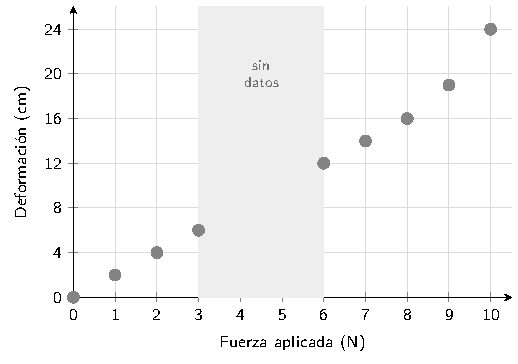
\includegraphics[max width=0.92\linewidth,max height=8.5cm]{fis/hab_hooke}
\end{center}
\altslargas{Se mantendrá en 6 cm, porque en ese tramo no hay datos.}{Disminuirá a medida que la fuerza aumente.}{Tomará valores entre 6 y 12 cm, de unos 2 cm por cada newton; por ejemplo, cerca de 9 cm con 4,5 N.}{Superará los 24 cm, porque el resorte habrá pasado su límite elástico.}
\solucion{\textbf{Paso 1. ¿Qué nos piden?} Estimar la deformación en un tramo sin datos, que está \textbf{dentro} del rango medido: es una interpolación.

\textbf{Paso 2. Mira la tendencia a ambos lados.} Con 1, 2 y 3 N la deformación es 2, 4 y 6 cm. Con 6, 7 y 8 N es 12, 14 y 16 cm. En ambos lados se cumple lo mismo: \textbf{2 cm por cada newton}, una recta que pasa por el origen.

\textbf{Paso 3. Aplica la tendencia al hueco.} Si con 3 N hay 6 cm y con 6 N hay 12 cm, entre medio la deformación irá de 6 a 12 cm. Con 4,5 N: $4{,}5\cdot 2 = 9$ cm.

\textbf{Respuesta:} tomará valores entre 6 y 12 cm, de unos 2 cm por cada newton.

\textbf{¿Por qué no las otras?} Que no haya datos no significa que el resorte deje de estirarse: entre 3 y 6 N la fuerza sigue aumentando. Que disminuya contradice la tendencia, que siempre es creciente. El cambio de comportamiento aparece recién sobre 8 N y con 10 N la deformación es 24 cm: con menos de 6 N no puede superarla.

\textbf{\color{cienciaD}Para recordar.} Para interpolar, sigue la tendencia de los puntos vecinos dentro del rango medido.}{C}
\end{elejemplo}

%% =====================================================================
%% fis_hab_evaluar
\section[Evaluar y comunicar]{Evaluar y comunicar}
\modcomun\ \ {\color{gris}\itshape Distinguir ley, teoría y modelo, reconocer los límites de un modelo (cuerda ideal, resistor óhmico, rayo de luz), evaluar la confiabilidad de las mediciones (repeticiones, precisión, error), juzgar si una conclusión es válida, replicar procedimientos, reconocer aplicaciones tecnológicas y elegir el recurso para comunicar resultados.\par}
\subsection{Ley, teoría y modelo}
\begin{center}\small
\begin{tabularx}{\linewidth}{@{}>{\raggedright\arraybackslash\hsize=0.42\hsize}X>{\raggedright\arraybackslash\hsize=1.29\hsize}X>{\raggedright\arraybackslash\hsize=1.29\hsize}X@{}}
\toprule
\textbf{Componente} & \textbf{Qué es} & \textbf{Ejemplos en física} \\
\midrule
\textbf{Ley} & Describe \textbf{qué pasa}: una regularidad que se cumple siempre en ciertas condiciones. Muchas veces es una relación matemática. & Ley de Hooke, $F = k\,x$. Ley de Ohm, $V = I\,R$. Ley de reflexión: el ángulo de incidencia es igual al de reflexión. Leyes de Newton. \\
\textbf{Teoría} & Explica \textbf{por qué pasa}: una explicación amplia, respaldada por muchas evidencias distintas. & Teoría de la tectónica de placas (explica sismos, volcanes y cordilleras). Teoría electromagnética de la luz. \\
\textbf{Modelo} & Una \textbf{representación simplificada} que sirve para explicar o predecir. & El rayo de luz. La cuerda ideal. El cuerpo como partícula. El modelo dinámico de las capas de la Tierra. La analogía del agua para la corriente. \\
\bottomrule
\end{tabularx}
\end{center}
  
\begin{clave}[{Cómo distinguirlas}] · «La deformación es proporcional a la fuerza»: dice qué pasa \ensuremath{\rightarrow} \textbf{ley}.\par · «Los continentes se mueven porque la litosfera está dividida en placas que se desplazan sobre la astenósfera»: explica por qué \ensuremath{\rightarrow} \textbf{teoría}.\par · «Consideremos la cuerda inextensible y sin masa»: simplifica para calcular \ensuremath{\rightarrow} \textbf{modelo}.\end{clave}
  
\begin{clave}[{Recuerda}] Una teoría no es «una suposición» ni se convierte en ley al acumular pruebas: la ley dice qué pasa y la teoría explica por qué. Son componentes distintos y ninguno pasa a ser el otro. Una teoría bien establecida, como la tectónica de placas, está respaldada por muchísima evidencia.\end{clave}
\subsection{Los modelos tienen límites}
Todo modelo deja algo afuera. Es útil mientras lo que deja afuera no importe; cuando importa, hay que cambiar de modelo.

 
\begin{center}\small
\begin{tabularx}{\linewidth}{@{}>{\raggedright\arraybackslash\hsize=0.62\hsize}X>{\raggedright\arraybackslash\hsize=1.19\hsize}X>{\raggedright\arraybackslash\hsize=1.19\hsize}X@{}}
\toprule
\textbf{Modelo} & \textbf{Supone} & \textbf{Deja de servir cuando\dots{}} \\
\midrule
Cuerda ideal & sin masa e inextensible: la misma tensión en toda la cuerda & la cuerda es gruesa y pesada: la tensión es mayor arriba que abajo \\
Resorte ideal (Hooke) & deformación proporcional a la fuerza & se supera el límite elástico \\
Resistor óhmico & resistencia constante & el conductor se calienta mucho, como el filamento de una ampolleta \\
Rayo de luz & la luz viaja en línea recta & la abertura es comparable a la longitud de onda: aparece la difracción \\
Sin roce & no hay fuerzas que se opongan al movimiento & las superficies son rugosas o el aire frena al objeto \\
\bottomrule
\end{tabularx}
\end{center}
  
\begin{center}
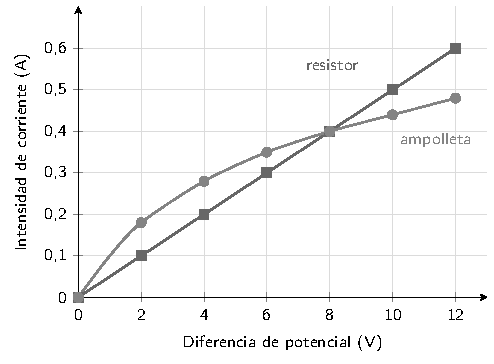
\includegraphics[max width=0.92\linewidth,max height=8.5cm]{fis/hab_no_ohmico}
\end{center}
 
\begin{ejemplo}[{Ejemplo resuelto}] ¿Cumple la ampolleta la ley de Ohm?\par \textbf{Paso 1.} Calcula $R = V/I$ en dos puntos: con 2 V, $\dfrac{2}{0{,}18}\approx 11$ \ensuremath{\Omega}; con 12 V, $\dfrac{12}{0{,}48} = 25$ \ensuremath{\Omega}.\par \textbf{Paso 2.} La resistencia cambia: aumenta porque el filamento se calienta.\par \textbf{Conclusión:} la ampolleta no es un resistor óhmico; la ley de Ohm, con $R$ constante, no la describe bien.\end{ejemplo}
\subsection{Validez, confiabilidad y error de medición}
\begin{center}
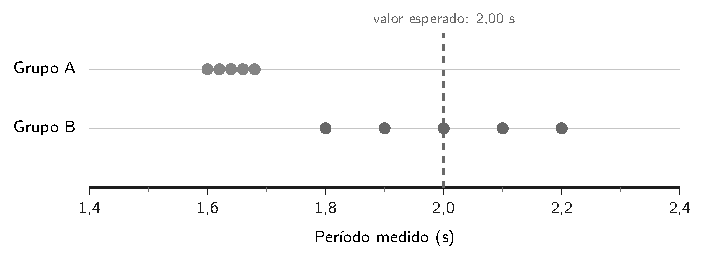
\includegraphics[max width=0.92\linewidth,max height=8.5cm]{fis/hab_mediciones}
\end{center}
  

\textbf{Validez:} la investigación mide de verdad lo que dice medir y su diseño permite responder la pregunta. Falla si cambian dos variables a la vez o si se mide otra variable.

 

\textbf{Confiabilidad:} al repetir la medición se obtienen resultados parecidos. Mejora con más repeticiones y con instrumentos más precisos.

 

\textbf{Precisión y exactitud.} Mediciones \textbf{precisas} están cerca unas de otras. Mediciones \textbf{exactas} están cerca del valor real. En la figura, el grupo A es preciso pero no exacto (quizás su cronómetro o su largo estaban mal); el grupo B tiene un promedio exacto, 2,00 s, pero es menos preciso.

  
\begin{ejemplo}[{Ejemplo resuelto: reducir el error}] Medir con cronómetro una sola oscilación de 2 s tiene un error de reacción de unos 0,2 s, un 10 \%.\par \textbf{Mejora:} medir el tiempo de 10 oscilaciones (unos 20 s) y dividir por 10. El error de reacción sigue siendo de unos 0,2 s, pero repartido en 10 oscilaciones: 0,02 s por oscilación, un 1 \%. Además, conviene repetir la medición y promediar.\end{ejemplo}
 
\begin{clave}[{Recuerda}] Repetir una medición con el mismo error de calibración no la hace exacta: la hace más confiable. Para corregir un error sistemático hay que revisar el instrumento o el montaje.\end{clave}
\subsection{¿La conclusión se sostiene con los datos?}
Para evaluar una conclusión, revisa esta lista:

 

\textbf{1. ¿Responde la pregunta?}

 

\textbf{2. ¿Habla solo de las variables medidas y del rango estudiado?} Si el resorte se probó hasta 5 N, no se puede afirmar qué pasa con 50 N.

 

\textbf{3. ¿Cambió solo una variable?} Si cambiaron dos a la vez, el efecto no se puede atribuir a una.

 

\textbf{4. ¿Hay suficientes repeticiones?}

 

\textbf{5. ¿Se confunde asociación con causa?} Que dos cosas ocurran juntas no prueba que una cause la otra.

  
\begin{ejemplo}[{Ejemplo resuelto}] Una persona pone 1 L de agua recién sacada del refrigerador en el hervidor A y 1 L de agua de la llave en el hervidor B. El agua de B hierve antes y concluye: «el hervidor B es más potente».\par \textbf{Paso 1.} ¿Qué diferencia a los ensayos? El hervidor \textbf{y} la temperatura inicial del agua.\par \textbf{Paso 2.} El agua más fría necesita más energía para llegar a 100 °C, así que puede tardar más aunque el hervidor sea igual de potente.\par \textbf{Evaluación:} la conclusión no se sostiene. Hay que repetir con la misma cantidad de agua a la misma temperatura inicial.\end{ejemplo}
 
\begin{clave}[{Recuerda}] Las alternativas correctas suelen ser prudentes: «en las condiciones del estudio», «en el rango medido», «podría». Desconfía de «siempre», «cualquier» y «demuestra».\end{clave}
\subsection{Replicar, reproducir y mejorar un diseño}
Un procedimiento es \textbf{replicable} si está descrito con tanto detalle que otra persona puede repetirlo. Un resultado es \textbf{reproducible} si al repetirlo se obtiene algo equivalente. Para replicar, hay que mantener las condiciones de las que depende el fenómeno, aunque cambien detalles que no influyen.

 
\begin{center}\small
\begin{tabularx}{\linewidth}{@{}>{\raggedright\arraybackslash\hsize=0.86\hsize}X>{\raggedright\arraybackslash\hsize=1.14\hsize}X@{}}
\toprule
\textbf{Limitación} & \textbf{Mejora} \\
\midrule
Una sola medición & Repetir y promediar. \\
Cambian dos variables a la vez & Cambiar solo la variable independiente. \\
Falta un ensayo de referencia & Medir también sin el factor estudiado. \\
Rango muy estrecho & Ampliar los valores de la variable independiente. \\
Instrumento poco preciso & Usar uno más preciso o medir un intervalo mayor (10 oscilaciones). \\
\bottomrule
\end{tabularx}
\end{center}
  
\begin{ejemplo}[{Ejemplo resuelto}] Un grupo observa el patrón de interferencia de un láser que pasa por dos rendijas muy finas y muy juntas en un papel. Quiere cambiar de láser y seguir viendo un patrón de interferencia. ¿Qué es indispensable mantener?\par \textbf{Paso 1.} ¿De qué depende la interferencia? De que la luz pase por dos aberturas muy pequeñas y cercanas, comparables con la longitud de onda.\par \textbf{Paso 2.} El color o la intensidad del láser cambian el aspecto del patrón (separación de franjas, brillo), pero no impiden que se forme.\par \textbf{Respuesta:} mantener rendijas igual de finas y con una separación similar.\end{ejemplo}
 
\begin{clave}[{Recuerda}] La mejora correcta corrige el defecto que impide responder la pregunta. Si el problema es que cambian dos variables, repetir más veces no lo resuelve.\end{clave}
\subsection{Aplicaciones tecnológicas y comunicar resultados}
\textbf{De la investigación a la tecnología.} La PAES pregunta qué tecnología usa un fenómeno o qué producto podría surgir de un hallazgo.

 
\begin{center}\small
\begin{tabularx}{\linewidth}{@{}>{\raggedright\arraybackslash\hsize=1.00\hsize}X>{\raggedright\arraybackslash\hsize=1.00\hsize}X@{}}
\toprule
\textbf{Fenómeno o hallazgo} & \textbf{Tecnología} \\
\midrule
Reflexión de ondas de radio & radar \\
Materiales piezoeléctricos (voltaje al presionarlos) & chisperos de cocinas y encendedores \\
Radiación infrarroja que emiten los cuerpos tibios & cámaras de visión nocturna \\
Material que bloquea un amplio espectro de radiación & recubrimientos para trajes de astronauta \\
Temperatura de ebullición menor a menor presión atmosférica & sensores de presión en hervidores \\
\bottomrule
\end{tabularx}
\end{center}
  
\begin{center}\small
\begin{tabularx}{\linewidth}{@{}>{\raggedright\arraybackslash\hsize=1.00\hsize}X>{\raggedright\arraybackslash\hsize=1.00\hsize}X@{}}
\toprule
\textbf{Objetivo al comunicar} & \textbf{Recurso} \\
\midrule
Mostrar cómo una variable depende de otra & gráfico de dispersión o de líneas, con la independiente en el eje horizontal \\
Comparar categorías (materiales, colores) & gráfico de barras \\
Entregar valores exactos & tabla \\
Explicar un fenómeno (difracción, refracción) & esquema o modelo del fenómeno \\
Mostrar cómo instalar o conectar algo & plano o diagrama del circuito \\
Informar a la población & afiche con recomendaciones claras \\
\bottomrule
\end{tabularx}
\end{center}
 
\begin{clave}[{Recuerda}] El recurso debe calzar con el objetivo. Si un equipo midió la intensidad de un láser y la profundidad del corte que produce, un gráfico de profundidad en función de la intensidad muestra justo su resultado; un esquema del montaje o una imagen de las ondas no.\end{clave}
\subsection{Lo clave del tema}
\begin{center}\small
\begin{tabularx}{\linewidth}{@{}>{\raggedright\arraybackslash\hsize=0.71\hsize}X>{\raggedright\arraybackslash\hsize=1.29\hsize}X@{}}
\toprule
\textbf{Si te piden\dots{}} & \textbf{Revisa esto} \\
\midrule
Ley, teoría o modelo & Qué pasa / por qué pasa / representación simplificada. \\
Límite de un modelo & Qué supone el modelo y qué dato lo contradice. \\
Confiabilidad & Repeticiones, precisión del instrumento, mediciones cercanas entre sí. \\
Validez & ¿Cambió solo una variable? ¿Se midió la variable del objetivo? \\
Evaluar una conclusión & ¿Sale de los datos? ¿Respeta el rango? ¿Hay variables confundidas? \\
Replicar & Mantener las condiciones de las que depende el fenómeno. \\
Comunicar & El recurso que muestra justo lo que se quiere mostrar. \\
\bottomrule
\end{tabularx}
\end{center}
 
\begin{clave}[{Recuerda}] · Una ley no se transforma en teoría ni al revés.\par · La cuerda ideal, el resorte ideal y el resistor óhmico son modelos con límites.\par · Precisas = cercanas entre sí; exactas = cercanas al valor real.\par · Medir varias oscilaciones y dividir reduce el error del cronómetro.\par · Si dos variables cambian a la vez, la conclusión no se sostiene.\end{clave}
 
\begin{clave}[{Método PAES}] 1. Identifica el objetivo y las variables del estudio. 2. Revisa el diseño: una sola variable cambiada, referencia, repeticiones, instrumento. 3. Compara la alternativa con los datos y con su rango. 4. Desconfía de «siempre», «todos», «cualquier» y «demuestra». 5. Si piden comunicar, elige el recurso según lo que se quiere mostrar.\end{clave}
\begin{elejemplo}{PAES Invierno 2027, adaptada}
Una persona que vive sola registra el consumo eléctrico mensual de su departamento y anota cuándo compra o cambia algún artefacto:

\begin{center}\small
\begin{tabular}{@{}llllllll@{}}
\toprule
\textbf{Mes} & \textbf{May.} & \textbf{Jun.} & \textbf{Jul.} & \textbf{Ago.} & \textbf{Sep.} & \textbf{Oct.} & \textbf{Nov.} \\
\midrule
Consumo (kWh) & 85,3 & 87,6 & 88,4 & 92,1 & 86,2 & 87,4 & 84,2 \\
\bottomrule
\end{tabular}
\end{center}

\textbf{Notas.} Inicio de junio: compré un televisor para ver una serie. Mediados de julio: cambié el refrigerador por uno nuevo que, según el fabricante, consume menos energía. Fines de noviembre: compré un ventilador.

A fin de año, decide reclamarle al fabricante del refrigerador porque no observa que su consumo haya disminuido. ¿Por qué se puede cuestionar su reclamo?
\altslargas{Porque el consumo de agosto es el mayor del registro, lo que prueba que el refrigerador nuevo consume más que el antiguo.}{Porque el registro no informa cuánto se usó cada artefacto cada mes y, en el mismo período, se agregó un televisor, así que no se puede aislar el efecto del refrigerador.}{Porque el ventilador comprado a fines de noviembre explica el aumento del consumo en agosto.}{Porque el consumo eléctrico de un hogar no depende de sus artefactos.}
\solucion{\textbf{Paso 1. ¿Qué nos piden?} Evaluar si los datos permiten concluir que el refrigerador nuevo no redujo el consumo.

\textbf{Paso 2. ¿Qué cambió en el período?} Desde junio hay un televisor nuevo, y a mediados de julio cambió el refrigerador. El consumo total depende de \textbf{todos} los artefactos y de cuánto se usa cada uno.

\textbf{Paso 3. ¿Se puede aislar el refrigerador?} No. El registro solo da el consumo total. Si el televisor se usó mucho (por ejemplo, para ver la serie), su consumo puede tapar el ahorro del refrigerador. Hay dos variables que cambiaron y no hay datos de uso de cada artefacto.

\textbf{Respuesta:} porque el registro no informa cuánto se usó cada artefacto y, en el mismo período, se agregó un televisor.

\textbf{Cómo mejorar:} medir el consumo del refrigerador por separado, o comparar meses con el mismo uso de los demás artefactos.

\textbf{¿Por qué no las otras?} Que agosto sea el mes de mayor consumo total no prueba nada sobre el refrigerador: puede deberse a otros artefactos o a más tiempo en casa. El ventilador se compró a fines de noviembre: no puede explicar agosto. El consumo de un hogar sí depende de sus artefactos; precisamente por eso hay que separar el efecto de cada uno.

\textbf{\color{cienciaD}Para recordar.} Si varias cosas cambian a la vez y solo se mide el total, no se puede atribuir el efecto a una sola.}{B}
\end{elejemplo}

%% Generado por html2tex.py desde temas.json (bio). No editar a mano: corregir la clase en el .js del sitio y regenerar.
\parteciencia{bio}
\chapter{Organización celular}
%% =====================================================================
%% bio_celulas
\section[Células procariontes y eucariontes]{Células procariontes y eucariontes}
\modcomun\ \ {\color{gris}\itshape La teoría celular, cómo son las células procariontes y eucariontes y qué estructuras tienen las células animales y vegetales: cápsula, pared celular, membrana, citoplasma, núcleo, ribosomas, cloroplastos y vacuola central.\par}
\subsection{La teoría celular}
En 1665, Robert Hooke miró una lámina de corcho con un microscopio sencillo y vio pequeñas cavidades que llamó \textbf{células}. Pocos años después, Anton van Leeuwenhoek, con lentes mejores, observó por primera vez organismos unicelulares vivos en gotas de agua.

 

Durante el siglo XIX, con microscopios más potentes, se reunieron las observaciones en la \textbf{teoría celular}:

 
\begin{itemize}
  \item \textbf{Todos los seres vivos están formados por una o más células} (Schleiden en plantas, 1838; Schwann en animales, 1839).
  \item \textbf{La célula es la unidad estructural y funcional} de los seres vivos: es la estructura más pequeña que cumple todas las funciones vitales.
  \item \textbf{Toda célula proviene de otra célula preexistente}, por división (Virchow, 1855).
  \item La célula contiene la \textbf{información hereditaria} (ADN), que pasa a las células hijas.
\end{itemize}
  
\begin{clave}[{Por qué tardó tanto}] Casi todas las células miden entre 1 y 100 µm (micrómetros), muy por debajo de lo que distingue el ojo (unos 100 µm). La teoría celular dependió del avance de la \textbf{microscopía}: sin lentes de buena calidad no había cómo observar ni comparar células.\end{clave}
 
\begin{ejemplo}[{Ejemplo resuelto}] En un cultivo, cada célula nueva aparece siempre por la división de una célula que ya existía; nunca a partir de materia sin vida. Esta observación apoya el postulado «toda célula proviene de otra célula preexistente».\end{ejemplo}
\subsection{Células procariontes}
Las \textbf{procariontes} (bacterias y arqueas) son las células más simples y pequeñas (1 a 10 µm). Su rasgo central: \textbf{no tienen núcleo}. Su ADN es una molécula circular que está en una zona del citoplasma llamada \textbf{nucleoide}. Tampoco tienen organelos rodeados por membrana.

 
\begin{itemize}
  \item \textbf{Membrana plasmática:} bicapa de fosfolípidos que regula qué entra y qué sale.
  \item \textbf{Pared celular:} capa rígida por fuera de la membrana; en las bacterias está hecha de \textbf{peptidoglicano}. Da forma y evita que la célula estalle al entrar agua. La penicilina actúa impidiendo su formación.
  \item \textbf{Cápsula:} capa externa de polisacáridos, presente en algunas bacterias. Las ayuda a adherirse a superficies y a evitar ser fagocitadas por los glóbulos blancos.
  \item \textbf{Ribosomas:} fabrican las proteínas (en bacterias son más pequeños que en eucariontes).
  \item \textbf{Plásmidos:} pequeñas moléculas de ADN circular extra, con genes como los de resistencia a antibióticos.
  \item \textbf{Flagelo} (movimiento) y \textbf{pili} (adherencia e intercambio de ADN).
\end{itemize}
  
\begin{center}
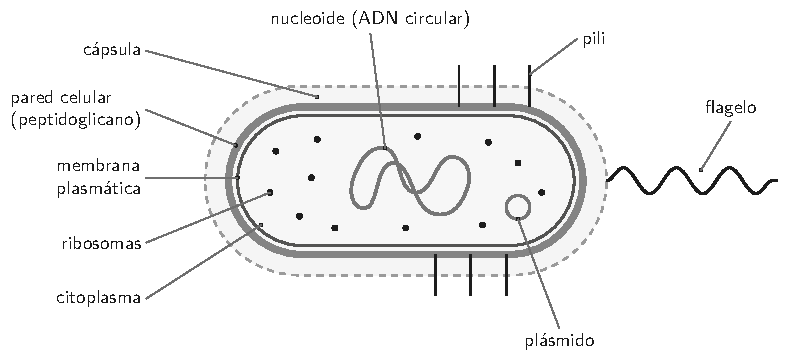
\includegraphics[max width=0.92\linewidth,max height=8.5cm]{bio/cel_procarionte}
\end{center}
\subsection{Células eucariontes}
Las \textbf{eucariontes} forman a los protistas, hongos, plantas y animales. Son más grandes (10 a 100 µm) y más complejas:

 
\begin{itemize}
  \item Tienen \textbf{núcleo}: el ADN está dentro de una envoltura de doble membrana con poros.
  \item Tienen \textbf{organelos rodeados por membrana}, cada uno con su tarea: retículo endoplasmático, complejo de Golgi, lisosomas, mitocondrias, cloroplastos (en plantas y algas), vacuolas.
  \item Tienen \textbf{citoesqueleto}, una red de filamentos de proteína que da forma, mueve organelos y permite el movimiento celular.
  \item Su ADN es lineal, está asociado a proteínas (histonas) y repartido en varios cromosomas.
\end{itemize}
 

Esta división del trabajo en compartimentos permite que en una misma célula ocurran a la vez procesos que necesitan condiciones distintas, como la digestión ácida en los lisosomas y la síntesis de proteínas en el citoplasma.

  
\begin{clave}[{La teoría endosimbiótica}] Lynn Margulis propuso que las \textbf{mitocondrias} y los \textbf{cloroplastos} fueron procariontes que otra célula incorporó sin digerirlos. Evidencias: tienen \textbf{doble membrana}, \textbf{ADN circular propio}, \textbf{ribosomas parecidos a los bacterianos} y se reproducen por \textbf{división} dentro de la célula.\end{clave}
\subsection{Célula animal y célula vegetal}
\begin{center}
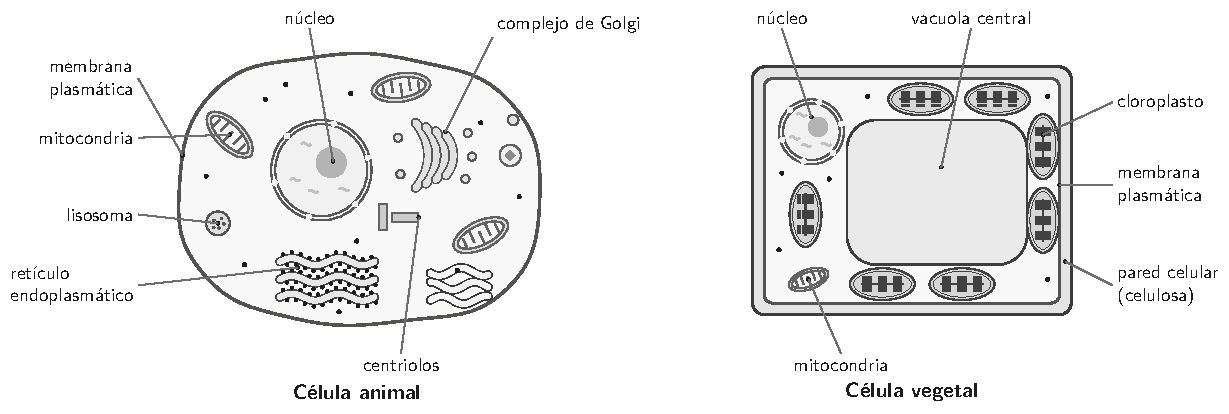
\includegraphics[max width=0.92\linewidth,max height=8.5cm]{bio/cel_animal_vegetal}
\end{center}
  

\textbf{Solo en la célula vegetal} (típica de una hoja):

 
\begin{itemize}
  \item \textbf{Pared celular de celulosa:} rígida, da forma y resiste la presión del agua.
  \item \textbf{Cloroplastos:} realizan la fotosíntesis.
  \item \textbf{Vacuola central grande:} guarda agua, iones y pigmentos; al llenarse empuja contra la pared y mantiene la célula firme (turgencia).
\end{itemize}
  

\textbf{Solo en la célula animal:}

 
\begin{itemize}
  \item \textbf{Centriolos} (las plantas con flor no los tienen).
  \item \textbf{Lisosomas} típicos; en las plantas, la vacuola cumple parte de la función digestiva.
  \item Forma variable, porque no hay pared.
\end{itemize}
 

\textbf{En ambas:} membrana plasmática, citoplasma, núcleo, ribosomas, retículo endoplasmático, complejo de Golgi y \textbf{mitocondrias}. Las plantas también respiran.
\subsection{Lo clave del tema}
\begin{center}\small
\begin{tabularx}{\linewidth}{@{}>{\raggedright\arraybackslash\hsize=0.87\hsize}X>{\raggedright\arraybackslash\hsize=1.20\hsize}X>{\raggedright\arraybackslash\hsize=0.93\hsize}X@{}}
\toprule
\textbf{Estructura} & \textbf{Función} & \textbf{Dónde está} \\
\midrule
Cápsula & adherencia; evitar la fagocitosis & algunas bacterias \\
Pared celular & forma y resistencia a la presión del agua & bacterias, hongos, plantas \\
Membrana plasmática & límite celular; regula el paso de sustancias & todas las células \\
Ribosomas & síntesis de proteínas & todas las células \\
Núcleo & guarda el ADN y controla la célula & eucariontes \\
Flagelo & movimiento & bacterias y algunas eucariontes \\
Cloroplasto / vacuola central & fotosíntesis / agua, reservas y turgencia & células vegetales \\
\bottomrule
\end{tabularx}
\end{center}
 
\begin{clave}[{Recuerda}] · Procarionte = sin núcleo y sin organelos membranosos; su ADN circular está en el nucleoide.\par · Las plantas tienen mitocondrias además de cloroplastos.\par · La pared bacteriana es de peptidoglicano; la vegetal, de celulosa.\par · Mitocondrias y cloroplastos tienen ADN propio y doble membrana: evidencia de la endosimbiosis.\end{clave}
 
\begin{clave}[{Método PAES}] 1. Si te preguntan por una estructura bacteriana, relaciona la función descrita (moverse, adherirse, resistir la fagocitosis, resistir la presión) con flagelo, pili, cápsula o pared. 2. En una célula vegetal, une el agua, los pigmentos y la turgencia con la vacuola central, y la fotosíntesis con los cloroplastos. 3. En preguntas de historia de la ciencia, relaciona cada observación con el postulado de la teoría celular que apoya y recuerda que todo dependió de la microscopía.\end{clave}
\begin{elejemplo}{PAES Invierno 2026, adaptada}
Unos microbiólogos estudian bacterias que nadan hacia las zonas del medio de cultivo donde hay más nutrientes. Obtienen una cepa mutante que crece y se divide con normalidad, pero que ya no logra desplazarse en el líquido: queda siempre en el mismo lugar donde se sembró.

¿Qué estructura bacteriana está alterada con mayor probabilidad en la cepa mutante?
\alts{La cápsula.}{El flagelo.}{El plásmido.}{Los ribosomas.}
\solucion{\textbf{Paso 1. ¿Qué nos piden?} La estructura relacionada con la función que se perdió: \textbf{desplazarse en un líquido}.

\textbf{Paso 2. Relaciona función y estructura.} En las bacterias, el movimiento en medios líquidos depende del \textbf{flagelo}, un filamento largo que gira como una hélice y empuja a la célula.

\textbf{Paso 3. Usa el resto de la información.} La mutante crece y se divide normal: su metabolismo, su ADN y su síntesis de proteínas funcionan. Solo perdió la movilidad.

\textbf{Respuesta:} el flagelo.

\textbf{¿Por qué no las otras?} La cápsula sirve para adherirse y evitar la fagocitosis, no para nadar. Los plásmidos llevan genes extra (por ejemplo, de resistencia a antibióticos). Si los ribosomas fallaran, la bacteria no podría fabricar proteínas y no crecería con normalidad.

\textbf{\color{cienciaD}Para recordar.} Moverse en un líquido: flagelo.}{B}
\end{elejemplo}
\motivacion{Toda vida empieza con una célula, y todo buen puntaje empieza con un tema. Ya diste el primer paso.}

%% =====================================================================
%% bio_organelos
\section[Organelos y estructuras celulares]{Organelos y estructuras celulares}
\modcomun\ \ {\color{gris}\itshape Estructura y función de membrana, citoesqueleto, núcleo, nucléolo, ribosomas, retículos endoplasmáticos, complejo de Golgi, lisosomas, peroxisomas, mitocondrias, cloroplastos, vacuolas, centriolos, cilios y flagelos; la ruta de síntesis y secreción de proteínas y cómo se estudia con marcaje radiactivo y organelos inhibidos.\par}
\subsection{Mapa de la célula eucarionte}
\begin{center}
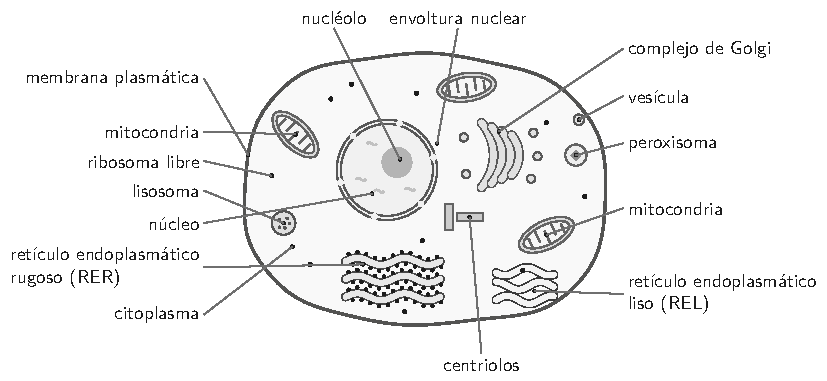
\includegraphics[max width=0.92\linewidth,max height=8.5cm]{bio/cel_organelos}
\end{center}
  

\textbf{Membrana plasmática.} Bicapa de fosfolípidos con proteínas y colesterol (en animales). Es \textbf{semipermeable}: deja pasar con facilidad algunas sustancias (O\textsubscript{2}, CO\textsubscript{2}, agua) y regula el paso de otras con proteínas transportadoras. Sus glicoproteínas permiten que las células se reconozcan.

  

\textbf{Organelos con membrana}: núcleo, retículos, Golgi, lisosomas, peroxisomas, vacuolas, mitocondrias y cloroplastos. \textbf{Estructuras sin membrana}: ribosomas, citoesqueleto, centriolos y nucléolo.

 

Tienen \textbf{doble membrana} el núcleo (envoltura nuclear), las mitocondrias y los cloroplastos.
\subsection{Citoesqueleto, centriolos, cilios y flagelos}
El \textbf{citoesqueleto} es una red de filamentos de proteína que recorre el citoplasma. Da forma a la célula, la hace resistente a fuerzas mecánicas, mueve los organelos y permite que la célula se desplace. Tiene tres tipos de filamentos:

 
\begin{itemize}
  \item \textbf{Microfilamentos} (actina): cambios de forma, emisión de pseudópodos, contracción muscular, división del citoplasma; sostienen las microvellosidades.
  \item \textbf{Filamentos intermedios} (como la queratina): resistencia a la tensión mecánica.
  \item \textbf{Microtúbulos} (tubulina): «rieles» por los que viajan vesículas y organelos; forman el \textbf{huso mitótico}, los cilios y los flagelos.
\end{itemize}
  

\textbf{Centriolos.} Par de cilindros de microtúbulos, perpendiculares entre sí, en el centrosoma de las células animales. Organizan los microtúbulos, por ejemplo durante la división celular.

 

\textbf{Cilios y flagelos.} Prolongaciones de la membrana con un esqueleto de microtúbulos que se mueven gastando ATP. Los \textbf{cilios} son cortos y numerosos: en la tráquea barren el mucus hacia arriba; en el oviducto mueven al ovocito. El \textbf{flagelo} es largo y suele ser único: mueve al espermatozoide.

 
\begin{clave}[{Recuerda}] Si un fármaco desarma los microtúbulos, se afectan a la vez el transporte de vesículas, la separación de cromosomas en la mitosis y el movimiento de cilios y flagelos.\end{clave}
\subsection{Núcleo, nucléolo y ribosomas}
\textbf{Núcleo.} Guarda el ADN y controla la actividad celular decidiendo qué genes se expresan. Está rodeado por la \textbf{envoltura nuclear}, de doble membrana, con \textbf{poros} por los que salen los ARN y entran proteínas. Dentro, el ADN está unido a proteínas (histonas) formando la \textbf{cromatina}.

 

\textbf{Nucléolo.} Zona del núcleo, sin membrana, donde se fabrica el \textbf{ARN ribosomal} y se arman las \textbf{subunidades de los ribosomas}, que luego salen al citoplasma por los poros. Las células que fabrican muchas proteínas tienen nucléolos grandes.

  

\textbf{Ribosomas.} Estructuras sin membrana, de ARN y proteínas, que \textbf{sintetizan proteínas} leyendo el ARN mensajero. Pueden estar:

 
\begin{itemize}
  \item \textbf{libres en el citoplasma:} hacen proteínas que se quedan en el citoplasma (por ejemplo, enzimas de la glucólisis);
  \item \textbf{adheridos al retículo endoplasmático rugoso:} hacen proteínas que se secretan (enzimas digestivas, hormonas como la insulina, anticuerpos), proteínas de membrana y enzimas de los lisosomas.
\end{itemize}
 
\begin{clave}[{Cadena de efectos}] Si se daña el nucléolo, se forman menos ribosomas; con menos ribosomas, con el tiempo baja la síntesis de proteínas. El efecto \textbf{directo} es el primero.\end{clave}
\subsection{Retículos endoplasmáticos y complejo de Golgi}
\textbf{Retículo endoplasmático rugoso (RER).} Sacos aplanados conectados con la envoltura nuclear y cubiertos de ribosomas. Allí se sintetizan las proteínas de secreción y de membrana; dentro del RER se pliegan y empiezan a modificarse. Luego salen en \textbf{vesículas de transporte} hacia el Golgi.

 

\textbf{Retículo endoplasmático liso (REL).} Túbulos sin ribosomas. Funciones:

 
\begin{itemize}
  \item síntesis de \textbf{lípidos}: fosfolípidos de membrana y \textbf{hormonas esteroidales} (testosterona, estrógenos, cortisol);
  \item \textbf{detoxificación} de fármacos, alcohol y otras sustancias, sobre todo en el hígado;
  \item almacenamiento de \textbf{calcio}: en el músculo se llama retículo sarcoplásmico.
\end{itemize}
  

\textbf{Complejo de Golgi.} Pila de sacos aplanados (cisternas). Recibe las proteínas del RER, las \textbf{modifica} (por ejemplo, les agrega azúcares), las \textbf{clasifica} y las \textbf{empaqueta} en vesículas según su destino: la membrana plasmática, los lisosomas o el exterior de la célula (secreción). En las plantas, además, fabrica componentes de la pared celular.

 
\begin{ejemplo}[{Ejemplo resuelto}] Las personas que toman por mucho tiempo ciertos fármacos tienen hepatocitos con el REL más desarrollado. Se explica porque el REL del hígado detoxifica esos fármacos: más fármaco, más REL.\end{ejemplo}
\subsection{Lisosomas, peroxisomas, vacuolas, mitocondrias y cloroplastos}
\begin{itemize}
  \item \textbf{Lisosomas:} vesículas con \textbf{enzimas digestivas} (hidrolasas) que trabajan en medio ácido. Digieren lo que la célula fagocita y reciclan organelos dañados (autofagia). Abundan en los glóbulos blancos fagocíticos.
  \item \textbf{Peroxisomas:} vesículas con enzimas oxidativas. Degradan ácidos grasos y sustancias tóxicas; en ese proceso se forma \textbf{peróxido de hidrógeno} (H\textsubscript{2}O\textsubscript{2}), que la enzima \textbf{catalasa} descompone en agua y oxígeno.
  \item \textbf{Vacuolas:} en plantas, una vacuola central grande guarda agua, iones, azúcares y pigmentos y mantiene la turgencia.
  \item \textbf{Mitocondrias:} hacen la \textbf{respiración celular}: usan glucosa (y otras moléculas) y O\textsubscript{2} para producir \textbf{ATP}, liberando CO\textsubscript{2} y agua. Abundan donde se gasta mucha energía.
  \item \textbf{Cloroplastos:} hacen la \textbf{fotosíntesis}: con la luz, convierten CO\textsubscript{2} y agua en glucosa y liberan O\textsubscript{2}.
\end{itemize}
  
\begin{center}
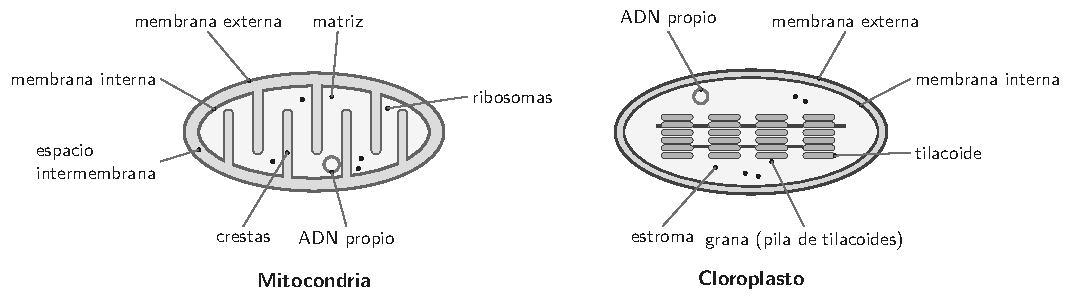
\includegraphics[max width=0.92\linewidth,max height=8.5cm]{bio/cel_mito_cloro}
\end{center}
 
\begin{clave}[{Recuerda}] Mitocondrias y cloroplastos tienen doble membrana, ADN y ribosomas propios. Las células vegetales tienen ambos organelos.\end{clave}
\subsection{La ruta de secreción y cómo se estudia}
\begin{center}
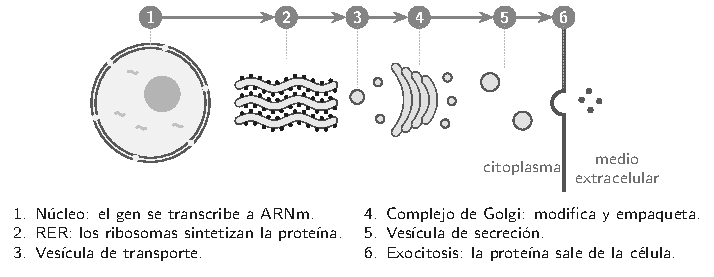
\includegraphics[max width=0.92\linewidth,max height=8.5cm]{bio/cel_secrecion}
\end{center}
  

\textbf{Marcaje radiactivo (pulso y caza).} Se entrega a las células, por pocos minutos, un aminoácido radiactivo (el \textbf{pulso}); luego se cambia por el mismo aminoácido sin marca (la \textbf{caza}). Las proteínas fabricadas durante el pulso quedan marcadas y se puede seguir dónde está la radiactividad a lo largo del tiempo: aparece primero en el \textbf{RER}, luego en el \textbf{Golgi} y al final en las \textbf{vesículas de secreción} y fuera de la célula.

  

\textbf{Organelos inhibidos.} Si un fármaco bloquea un paso, la proteína se \textbf{acumula en el compartimento anterior} al bloqueo y no llega a los siguientes. Por ejemplo, si se bloquea el paso del RER al Golgi, la marca queda en el RER; si se bloquea la salida del Golgi, la marca se acumula en el Golgi y no aparecen vesículas de secreción marcadas.

 
\begin{clave}[{Recuerda}] Para saber qué paso está bloqueado, busca el último compartimento donde la marca se acumula: el bloqueo está justo a la salida de ese compartimento.\end{clave}
\subsection{Lo clave del tema}
\begin{center}\small
\begin{tabularx}{\linewidth}{@{}>{\raggedright\arraybackslash\hsize=0.52\hsize}X>{\raggedright\arraybackslash\hsize=1.29\hsize}X>{\raggedright\arraybackslash\hsize=1.19\hsize}X@{}}
\toprule
\textbf{Organelo} & \textbf{Función principal} & \textbf{Si falla\dots{}} \\
\midrule
Nucléolo & arma subunidades de ribosomas & menos ribosomas \\
RER & sintetiza proteínas de secreción y de membrana & no se forman esas proteínas \\
REL & lípidos, esteroides, detoxificación, Ca\textsuperscript{2+} & se acumulan tóxicos; menos esteroides \\
Golgi & modifica, clasifica y empaqueta & proteínas retenidas, sin secretar \\
Lisosoma & digestión intracelular & material sin digerir acumulado \\
Peroxisoma & oxida ácidos grasos; degrada H\textsubscript{2}O\textsubscript{2} & acumulación de H\textsubscript{2}O\textsubscript{2} \\
Mitocondria & respiración celular: ATP & menos O\textsubscript{2} consumido y menos ATP \\
Citoesqueleto & forma, transporte interno, movimiento & la célula no migra ni mueve vesículas \\
\bottomrule
\end{tabularx}
\end{center}
 
\begin{clave}[{Método PAES}] 1. Subraya el efecto observado (menos ATP, H\textsubscript{2}O\textsubscript{2} acumulado, no se mueve, no secreta). 2. Pregúntate qué organelo produce o controla eso. 3. En experimentos de marcaje, sigue la ruta RER \ensuremath{\rightarrow} Golgi \ensuremath{\rightarrow} vesículas \ensuremath{\rightarrow} membrana y busca dónde se detiene la marca. 4. Distingue el efecto \textbf{directo} (el primero) de las consecuencias posteriores.\end{clave}
\begin{elejemplo}{PAES Invierno 2027, adaptada}
Para estudiar cómo se secretan las enzimas digestivas, se incubaron cortes de páncreas durante 3 minutos con un aminoácido radiactivo (pulso) y luego con el mismo aminoácido sin marca. A distintos tiempos se midió qué porcentaje de la radiactividad de las proteínas estaba en cada compartimento celular:
\begin{center}
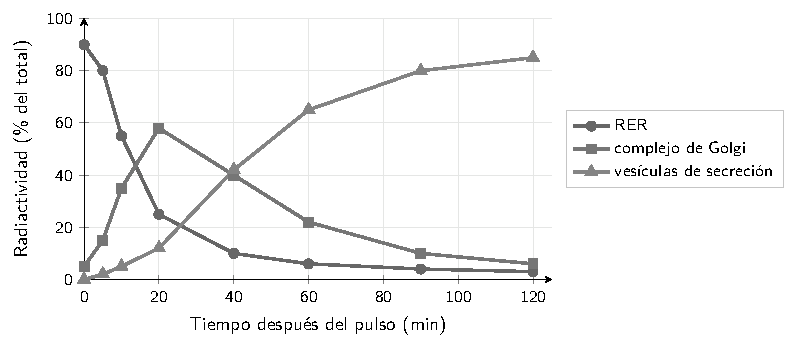
\includegraphics[max width=0.92\linewidth,max height=8.5cm]{bio/cel_pulso}
\end{center}
\altslargas{Las proteínas de secreción se sintetizan en el complejo de Golgi y luego pasan al RER.}{Las proteínas de secreción pasan del RER al complejo de Golgi y luego a las vesículas de secreción.}{Las vesículas de secreción sintetizan proteínas a partir del aminoácido marcado.}{La radiactividad desaparece de la célula a los 20 minutos.}
\solucion{\textbf{Paso 1. ¿Qué nos piden?} La conclusión que se desprende del orden en que la marca pasa por los compartimentos.

\textbf{Paso 2. Busca dónde está la marca al inicio.} Justo después del pulso, cerca del 90 \% de la radiactividad está en el \textbf{RER}: ahí se sintetizaron las proteínas con el aminoácido marcado.

\textbf{Paso 3. Sigue los máximos.} La marca del RER baja mientras sube la del \textbf{Golgi}, que llega a su máximo a los 20 minutos. Luego baja la del Golgi y sube la de las \textbf{vesículas de secreción}, que a los 120 minutos tienen el 85 \%.

\textbf{Respuesta:} las proteínas pasan del RER al complejo de Golgi y luego a las vesículas de secreción.

\textbf{¿Por qué no las otras?} El Golgi alcanza su máximo \textbf{después} que el RER, así que el orden es RER \ensuremath{\rightarrow} Golgi, no al revés. Las vesículas no sintetizan proteínas: reciben la marca al final, cuando ya pasó por el RER y el Golgi. La radiactividad no desaparece: a los 20 minutos está repartida entre RER, Golgi y vesículas, y la suma sigue cerca del 100 \%.

\textbf{\color{cienciaD}Para recordar.} El orden de los máximos de marca revela la ruta: RER \ensuremath{\rightarrow} Golgi \ensuremath{\rightarrow} vesículas de secreción.}{B}
\end{elejemplo}
\motivacion{Cada organelo hace su parte para que la célula funcione. Igual tú: cada tema estudiado suma al resultado final.}

%% =====================================================================
%% bio_especializadas
\section[Estructura y función: células especializadas]{Estructura y función: células especializadas}
\modcomun\ \ {\color{gris}\itshape Cómo la forma y los organelos de una célula se relacionan con su función: el enterocito y la célula secretora pancreática, y cómo deducir la función de una célula a partir de tablas y gráficos con la abundancia de sus organelos.\par}
\subsection{La estructura se ajusta a la función}
Casi todas las células de tu cuerpo tienen el mismo ADN, pero no son iguales: durante el desarrollo, cada tipo celular \textbf{expresa genes distintos} y se \textbf{especializa}. El resultado es que su forma y la cantidad de cada organelo calzan con lo que hace.

 

La idea clave para la PAES: \textbf{una célula tiene en abundancia los organelos que más usa}. Si sabes qué hace cada organelo, puedes deducir la función de una célula que nunca has visto, y al revés.

  
\begin{center}\small
\begin{tabularx}{\linewidth}{@{}>{\raggedright\arraybackslash\hsize=1.07\hsize}X>{\raggedright\arraybackslash\hsize=0.93\hsize}X@{}}
\toprule
\textbf{Si la célula\dots{}} & \textbf{tendrá muchos\dots{}} \\
\midrule
secreta proteínas (enzimas, hormonas proteicas, anticuerpos) & RER, Golgi y vesículas de secreción \\
fabrica hormonas esteroidales o detoxifica & REL \\
gasta mucha energía & mitocondrias \\
digiere lo que fagocita & lisosomas \\
absorbe sustancias & microvellosidades (más superficie) \\
se mueve o mueve líquidos & flagelo o cilios \\
\bottomrule
\end{tabularx}
\end{center}
\subsection{El enterocito: una célula para absorber}
Los \textbf{enterocitos} recubren el interior del intestino delgado y absorben los nutrientes ya digeridos (glucosa, aminoácidos, ácidos grasos) para pasarlos a la sangre.

 
\begin{itemize}
  \item \textbf{Microvellosidades:} miles de pliegues de la membrana en el polo que da a la luz del intestino (borde en cepillo). Multiplican la superficie de absorción; sostenidas por microfilamentos de actina.
  \item \textbf{Muchas mitocondrias:} parte de la absorción es \textbf{transporte activo} y gasta ATP; por ejemplo, la bomba de sodio y potasio mantiene el gradiente que permite absorber glucosa.
  \item \textbf{Uniones estrechas:} sellan el espacio entre células vecinas, así las sustancias pasan \textbf{a través} de las células y no entre ellas.
  \item \textbf{REL y Golgi:} rearman las grasas absorbidas y las empaquetan para enviarlas a la linfa.
\end{itemize}
  
\begin{center}
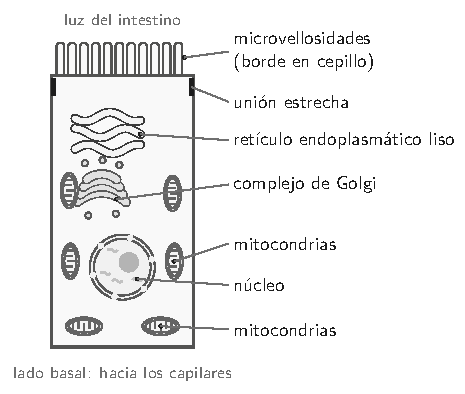
\includegraphics[max width=0.92\linewidth,max height=8.5cm]{bio/cel_enterocito}
\end{center}
\subsection{La célula acinar del páncreas: una célula para secretar}
Las \textbf{células acinares} del páncreas fabrican las enzimas digestivas del jugo pancreático. Tienen forma de pirámide truncada y una organización \textbf{polarizada}, de la base al ápice, que sigue la ruta de secreción:

 
\begin{itemize}
  \item \textbf{Base:} el núcleo y un \textbf{RER muy abundante}, donde se sintetizan las enzimas. El nucléolo es grande: se necesitan muchos ribosomas.
  \item \textbf{Sobre el núcleo:} un \textbf{complejo de Golgi} desarrollado, que modifica y empaqueta las enzimas.
  \item \textbf{Ápice:} muchos \textbf{gránulos de secreción} llenos de enzimas inactivas, que se liberan por exocitosis a la luz del acino.
\end{itemize}
 

Las células beta de los islotes del páncreas también son secretoras de proteínas (insulina) y muestran el mismo patrón: RER y Golgi abundantes.

  
\begin{center}
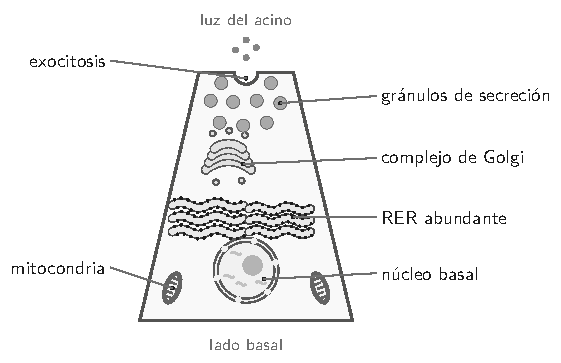
\includegraphics[max width=0.92\linewidth,max height=8.5cm]{bio/cel_acinar}
\end{center}
\subsection{Leer tablas y gráficos de organelos}
Muchas preguntas entregan una tabla o un gráfico con el \textbf{porcentaje del volumen celular} que ocupa cada organelo en varias células, y piden deducir su función. El procedimiento:

 
\begin{itemize}
  \item \textbf{1.} Para cada célula, busca el organelo que \textbf{destaca} respecto de las demás células.
  \item \textbf{2.} Traduce ese organelo a su función (usa la tabla de la primera diapositiva).
  \item \textbf{3.} Une esa función con el tipo de célula que la necesita.
\end{itemize}
 

Algunas parejas que conviene conocer:

 
\begin{itemize}
  \item \textbf{Célula plasmática} (secreta anticuerpos): RER y Golgi.
  \item \textbf{Células de Leydig} del testículo y de la corteza suprarrenal (hormonas esteroidales): REL.
  \item \textbf{Hepatocito:} REL (detoxificación), mitocondrias y peroxisomas.
  \item \textbf{Neutrófilos y macrófagos} (fagocitan): lisosomas.
\end{itemize}
  
\begin{ejemplo}[{Ejemplo resuelto}] En una célula las mitocondrias ocupan el 35 \% del volumen y en otra, el 6 \%. La primera tiene una capacidad mucho mayor de producir ATP: corresponde a una célula con alto gasto de energía sostenido, como las del músculo de vuelo de un ave que migra sin detenerse.\end{ejemplo}
 
\begin{clave}[{Recuerda}] Compara siempre entre células: un 8 \% de mitocondrias puede ser «mucho» o «poco» según con qué lo compares. Y lee bien las unidades del eje.\end{clave}
\subsection{Lo clave del tema}
\begin{center}\small
\begin{tabularx}{\linewidth}{@{}>{\raggedright\arraybackslash\hsize=0.80\hsize}X>{\raggedright\arraybackslash\hsize=0.93\hsize}X>{\raggedright\arraybackslash\hsize=1.28\hsize}X@{}}
\toprule
\textbf{Célula} & \textbf{Función} & \textbf{Estructuras destacadas} \\
\midrule
Enterocito & absorber nutrientes & microvellosidades, mitocondrias, uniones estrechas \\
Célula acinar pancreática & secretar enzimas & RER y Golgi abundantes, gránulos de secreción apicales \\
Célula plasmática & secretar anticuerpos & RER y Golgi abundantes \\
Célula de Leydig & fabricar testosterona & REL abundante \\
Neutrófilo & fagocitar y digerir bacterias & lisosomas abundantes \\
\bottomrule
\end{tabularx}
\end{center}
 
\begin{clave}[{Recuerda}] · Las microvellosidades aumentan la superficie de absorción.\par · Muchas mitocondrias indican un alto gasto de ATP, por ejemplo para el transporte activo o un trabajo sostenido.\par · En una célula secretora, el orden de base a ápice es núcleo y RER \ensuremath{\rightarrow} Golgi \ensuremath{\rightarrow} gránulos.\end{clave}
 
\begin{clave}[{Método PAES}] 1. Identifica el organelo o la estructura que destaca. 2. Recuerda su función. 3. Elige la célula o la función que necesita esa estructura. 4. En experimentos, pregúntate qué pasa si esa estructura falta o se daña: su función disminuye.\end{clave}
\begin{elejemplo}{PAES Invierno 2026, adaptada}
Un grupo de investigadores midió, en tres tipos celulares, qué porcentaje del volumen de la célula ocupan cuatro organelos. Los resultados (datos hipotéticos) se muestran en el gráfico:

¿Qué asociación entre célula y función es más coherente con estos datos?
\begin{center}
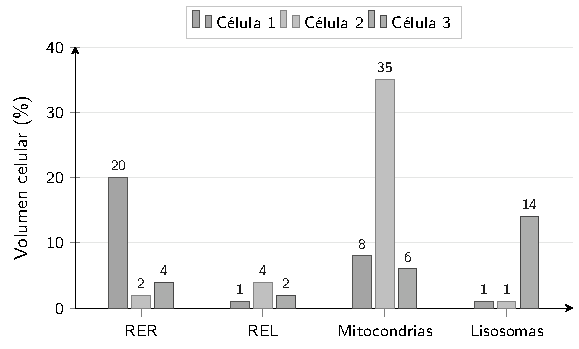
\includegraphics[max width=0.92\linewidth,max height=8.5cm]{bio/cel_vol_1}
\end{center}
\altslargas{Célula 1: secreción de enzimas digestivas.}{Célula 2: síntesis de hormonas esteroidales.}{Célula 3: contracción sostenida con alto gasto de ATP.}{Célula 1: digestión de bacterias fagocitadas.}
\solucion{\textbf{Paso 1. ¿Qué nos piden?} Relacionar el organelo que destaca en cada célula con una función.

\textbf{Paso 2. Busca lo que destaca.} Célula 1: el \textbf{RER} (20 \%, mucho más que en las otras). Célula 2: las \textbf{mitocondrias} (35 \%). Célula 3: los \textbf{lisosomas} (14 \%).

\textbf{Paso 3. Traduce a funciones.} Mucho RER \ensuremath{\rightarrow} síntesis de proteínas para secretar, como las enzimas digestivas. Muchas mitocondrias \ensuremath{\rightarrow} alto gasto de ATP, como en un músculo que se contrae sin pausa. Muchos lisosomas \ensuremath{\rightarrow} digestión intracelular, como en una célula que fagocita bacterias.

\textbf{Respuesta:} célula 1: secreción de enzimas digestivas.

\textbf{¿Por qué no las otras?} La síntesis de hormonas esteroidales necesita mucho REL, y la célula 2 tiene apenas 4 \%. La contracción sostenida corresponde a la célula 2 (mitocondrias), no a la 3. La digestión de bacterias fagocitadas corresponde a la célula 3 (lisosomas), no a la 1.

\textbf{\color{cienciaD}Para recordar.} Organelo que destaca \ensuremath{\rightarrow} función: RER = secretar proteínas; mitocondrias = gastar energía; lisosomas = digerir.}{A}
\end{elejemplo}
\motivacion{Forma y función van de la mano: ya entiendes por qué una neurona no se parece a un glóbulo rojo. ¡Excelente!}

\chapter{Procesos y funciones biológicas}
%% =====================================================================
%% bio_neurona
\section[Organización del sistema nervioso]{Organización del sistema nervioso}
\modcomun\ \ {\color{gris}\itshape Cómo coordina el sistema nervioso las respuestas del cuerpo frente a los estímulos y cómo se organiza: sistema nervioso central y periférico, divisiones somática y autónoma, y acciones opuestas de las divisiones simpática y parasimpática.\par}
\subsection{Cómo se organiza el sistema nervioso}
El sistema nervioso \textbf{coordina e integra} lo que hace el cuerpo frente a los \textbf{estímulos}, tanto externos (luz, sonido, calor) como internos (falta de agua, aumento de CO\textsubscript{2}). Cumple tres funciones en cadena:

 
\begin{itemize}
  \item \textbf{Sensitiva:} los receptores captan el estímulo.
  \item \textbf{Integradora:} el sistema nervioso central procesa la información y elabora una respuesta.
  \item \textbf{Motora:} la respuesta llega a un \textbf{efector}, un músculo o una glándula.
\end{itemize}
 

\textbf{Sistema nervioso central (SNC):} encéfalo (cerebro, cerebelo y tronco encefálico) y médula espinal. Está protegido por el cráneo, la columna vertebral, las meninges y el líquido cefalorraquídeo.

 

\textbf{Sistema nervioso periférico (SNP):} los nervios (12 pares craneales y 31 pares raquídeos) y los ganglios. Conecta el SNC con el resto del cuerpo.

  
\begin{clave}[{Las divisiones del SNP}] · \textbf{Somático:} controla los músculos esqueléticos; es voluntario (levantar la mano, caminar).\par · \textbf{Autónomo:} controla el corazón, el músculo liso y las glándulas; es involuntario.\par · \textbf{Simpático:} prepara para la acción, «lucha o huida»: aumenta la frecuencia cardíaca, dilata las pupilas y los bronquios, frena la digestión.\par · \textbf{Parasimpático:} «reposo y digestión»: baja la frecuencia cardíaca, contrae las pupilas, estimula la salivación y los movimientos del tubo digestivo.\end{clave}
  
\begin{center}
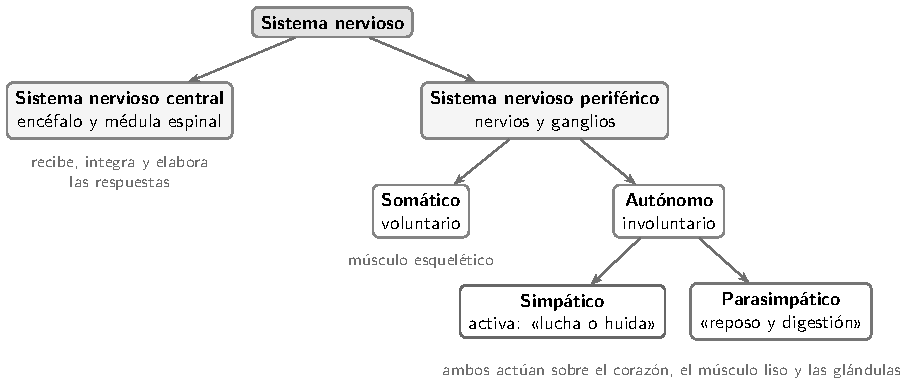
\includegraphics[max width=0.92\linewidth,max height=8.5cm]{bio/ner_organizacion}
\end{center}
\subsection{Lo clave del tema}
\begin{center}\small
\begin{tabularx}{\linewidth}{@{}>{\raggedright\arraybackslash\hsize=0.74\hsize}X>{\raggedright\arraybackslash\hsize=1.13\hsize}X>{\raggedright\arraybackslash\hsize=1.13\hsize}X@{}}
\toprule
\textbf{Parte} & \textbf{Qué incluye} & \textbf{Qué hace} \\
\midrule
SNC & encéfalo (cerebro, cerebelo, tronco encefálico) y médula espinal & integra la información y elabora respuestas \\
SNP somático & nervios hacia y desde la piel y los músculos esqueléticos & sensibilidad y movimiento voluntario \\
SNP autónomo simpático & nervios hacia el corazón, el músculo liso y las glándulas & «lucha o huida»: sube la frecuencia cardíaca, dilata pupilas y bronquios, frena la digestión \\
SNP autónomo parasimpático & nervios hacia los mismos órganos & «reposo y digestión»: baja la frecuencia cardíaca, contrae las pupilas, estimula la digestión \\
\bottomrule
\end{tabularx}
\end{center}
 
\begin{clave}[{Recuerda}] · Funciones en cadena: sensitiva (receptor) \ensuremath{\rightarrow} integradora (SNC) \ensuremath{\rightarrow} motora (efector: músculo o glándula).\par · SNC = encéfalo y médula espinal; SNP = nervios y ganglios.\par · El somático es voluntario; el autónomo es involuntario.\par · El simpático activa («lucha o huida»); el parasimpático favorece el reposo y la digestión.\end{clave}
 
\begin{clave}[{Método PAES}] 1. Pregúntate si la respuesta es voluntaria (somático) o involuntaria (autónomo). 2. Si es involuntaria, decide si prepara para la acción (simpático) o para el reposo y la digestión (parasimpático). 3. Para ubicar una estructura, recuerda que el SNC es solo encéfalo y médula espinal: todo nervio o ganglio es SNP.\end{clave}
\begin{elejemplo}{Estilo PAES}
Una persona camina de noche por una calle oscura y escucha un ruido fuerte detrás de ella. En pocos segundos su corazón late más rápido, sus pupilas se dilatan y su respiración se acelera. Estas respuestas son involuntarias.

¿Qué parte del sistema nervioso produce principalmente estas respuestas?
\altslargas{La división simpática del sistema nervioso autónomo.}{La división parasimpática del sistema nervioso autónomo.}{El sistema nervioso somático.}{El cerebelo, que coordina el equilibrio.}
\solucion{\textbf{Paso 1. ¿Qué nos piden?} La división que controla respuestas \textbf{involuntarias} que preparan al cuerpo frente a un peligro.

\textbf{Paso 2. Involuntario \ensuremath{\rightarrow} autónomo.} El corazón, el músculo de la pupila y los bronquios no se controlan a voluntad: los regula el sistema nervioso autónomo.

\textbf{Paso 3. ¿Cuál de sus divisiones?} Aumentar la frecuencia cardíaca, dilatar las pupilas y acelerar la respiración son respuestas de «lucha o huida»: las produce la división \textbf{simpática}.

\textbf{Respuesta:} la división simpática del sistema nervioso autónomo.

\textbf{¿Por qué no las otras?} La división parasimpática hace lo contrario: baja la frecuencia cardíaca y contrae las pupilas. El sistema somático controla los músculos esqueléticos de forma voluntaria. El cerebelo coordina el equilibrio y los movimientos, no el ritmo cardíaco ni las pupilas.

\textbf{\color{cienciaD}Para recordar.} Respuestas involuntarias de alerta («lucha o huida») = simpático.}{A}
\end{elejemplo}
\motivacion{Tu sistema nervioso acaba de aprender cómo funciona el sistema nervioso. ¡Eso sí que es pensar!}

%% =====================================================================
%% bio_sinapsis
\section[Arco reflejo, drogas y cuidado del sistema nervioso]{Arco reflejo, drogas y cuidado del sistema nervioso}
\modcomun\ \ {\color{gris}\itshape Cómo funciona el arco reflejo simple, qué efectos tienen la cafeína, el alcohol y las drogas de abuso sobre el sistema nervioso y qué cuidados lo protegen: dormir lo suficiente y prevenir traumatismos.\par}
\subsection{El arco reflejo}
Un \textbf{reflejo} es una respuesta \textbf{rápida, involuntaria y predecible} frente a un estímulo: retirar la mano de una olla caliente, el reflejo rotuliano, el parpadeo. El camino que sigue el impulso es el \textbf{arco reflejo}, con cinco componentes:

 
\begin{itemize}
  \item \textbf{Receptor:} capta el estímulo (en la piel, un receptor de dolor o de calor).
  \item \textbf{Vía aferente:} una neurona sensitiva lleva el impulso hacia el SNC. Entra a la médula por la raíz dorsal; su soma está en un ganglio.
  \item \textbf{Centro elaborador:} la médula espinal (o el tronco encefálico). Ahí la información pasa, a menudo a través de una interneurona, a una neurona motora.
  \item \textbf{Vía eferente:} una neurona motora lleva la orden hacia el efector.
  \item \textbf{Efector:} el músculo que se contrae o la glándula que secreta.
\end{itemize}
  
\begin{clave}[{¿Por qué es tan rápido?}] La respuesta se elabora en la médula, pasando por muy pocas neuronas, sin esperar al encéfalo. Al mismo tiempo, la información sube por la médula hasta el encéfalo: por eso sientes el dolor un instante \textbf{después} de haber retirado la mano.\end{clave}
 
\begin{clave}[{Recuerda}] El reflejo rotuliano es el arco más simple: la neurona sensitiva se conecta directamente con la neurona motora, sin interneurona.\end{clave}
  
\begin{center}
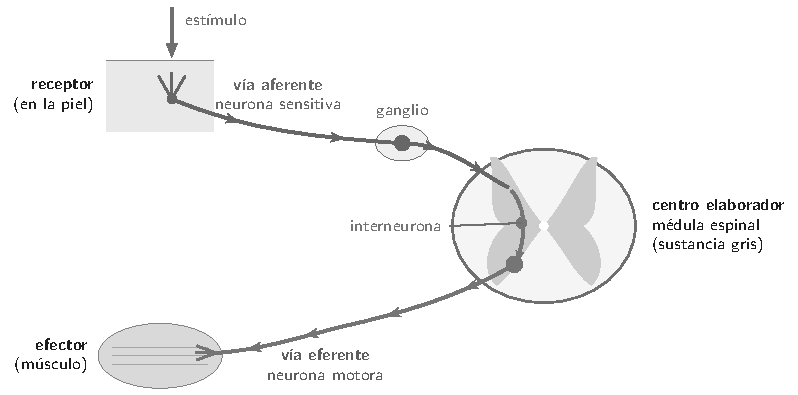
\includegraphics[max width=0.92\linewidth,max height=8.5cm]{bio/ner_arco}
\end{center}
\subsection{El café y la cafeína}
Mientras estamos despiertos, la actividad del encéfalo acumula \textbf{adenosina}. La adenosina se une a sus receptores en las neuronas y \textbf{disminuye} su actividad: así aparece la sensación de cansancio y sueño.

 

La \textbf{cafeína} (del café, el té, el mate, las bebidas cola y las bebidas energéticas) tiene una forma parecida a la adenosina. Se une a los receptores de adenosina \textbf{sin activarlos} y los bloquea. Resultado: la adenosina no puede actuar, y la persona se siente más alerta y con menos sueño.

 

La cafeína tarda unas 5 horas en reducirse a la mitad en la sangre. Por eso un café en la tarde puede retrasar el sueño en la noche.

  
\begin{clave}[{Efectos del consumo alto}] Insomnio, nerviosismo, ansiedad, taquicardia y molestias digestivas. Con el consumo diario aparece \textbf{tolerancia} (se necesita más para el mismo efecto), y al suspenderlo puede haber dolor de cabeza y cansancio por un par de días.\end{clave}
  
\begin{center}
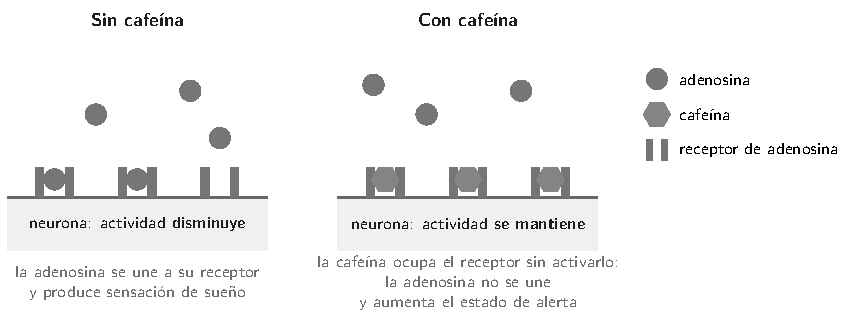
\includegraphics[max width=0.92\linewidth,max height=8.5cm]{bio/ner_cafeina}
\end{center}
\subsection{Alcohol y drogas de abuso}
Muchas sustancias alteran el funcionamiento del sistema nervioso y, con él, la conducta. Algunas lo \textbf{deprimen}: hacen más lentas sus respuestas. Otras lo \textbf{estimulan}: aumentan la alerta y la actividad.

 
\begin{center}\small
\begin{tabularx}{\linewidth}{@{}>{\raggedright\arraybackslash\hsize=0.63\hsize}X>{\raggedright\arraybackslash\hsize=0.79\hsize}X>{\raggedright\arraybackslash\hsize=1.58\hsize}X@{}}
\toprule
\textbf{Sustancia} & \textbf{Tipo} & \textbf{Efectos} \\
\midrule
Alcohol (etanol) & depresor del SNC & reflejos más lentos, falta de coordinación, peor juicio; en dosis altas, pérdida de conciencia y depresión respiratoria \\
Nicotina & estimulante & aumenta la alerta y la frecuencia cardíaca; muy adictiva \\
Cocaína & estimulante & euforia, taquicardia, hipertensión; alto riesgo de adicción \\
Anfetaminas & estimulantes & alerta, insomnio, taquicardia \\
Marihuana (THC) & altera la percepción & afecta la memoria, la atención y la coordinación \\
\bottomrule
\end{tabularx}
\end{center}
 
\begin{clave}[{Tolerancia y dependencia}] Las drogas de abuso activan el \textbf{circuito de recompensa} del encéfalo, el que produce la sensación de placer. Con el consumo repetido, el encéfalo se adapta: aparece la \textbf{tolerancia} (se necesita más droga para el mismo efecto), y al dejar la sustancia, el \textbf{síndrome de abstinencia}. Este cambio en el circuito de recompensa es la base de la adicción.\end{clave}
 
\begin{clave}[{Alcohol y conducción en Chile}] La ley considera «bajo la influencia del alcohol» a quien conduce con más de 0,3 g de alcohol por litro de sangre, y «en estado de ebriedad» desde 0,8 g/L. El alcohol alarga el tiempo de reacción incluso en dosis bajas.\end{clave}
\subsection{Cuidar el sistema nervioso}
\textbf{Dormir lo suficiente.} Durante el sueño el encéfalo consolida lo aprendido en el día (la memoria) y se recupera. Dormir poco empeora la atención, la memoria, el ánimo y el tiempo de reacción.

 
\begin{center}\small
\begin{tabular}{@{}ll@{}}
\toprule
\textbf{Edad} & \textbf{Horas de sueño recomendadas} \\
\midrule
6 a 12 años & 9 a 12 h \\
13 a 18 años & 8 a 10 h \\
Adultos & 7 a 9 h \\
\bottomrule
\end{tabular}
\end{center}
 

Ayudan a dormir bien: horarios regulares, evitar pantallas antes de acostarse y no tomar cafeína en la tarde.

  

\textbf{Prevenir traumatismos.} Las neuronas del SNC casi no se reemplazan cuando mueren: un daño en el encéfalo o en la médula espinal suele dejar secuelas permanentes.

 
\begin{itemize}
  \item \textbf{Traumatismo encéfalo craneano (TEC):} golpe en la cabeza en accidentes de tránsito, caídas o deportes. Se previene con \textbf{casco} (bicicleta, scooter, moto, esquí) y \textbf{cinturón de seguridad}, y con sillas para niños en el auto.
  \item \textbf{Lesión de la médula espinal:} se pierde la sensibilidad y el movimiento voluntario de las zonas del cuerpo que dependen de la médula bajo la lesión. Una causa frecuente en verano es lanzarse de cabeza en aguas poco profundas.
\end{itemize}
\subsection{Lo clave del tema}
\begin{center}\small
\begin{tabularx}{\linewidth}{@{}>{\raggedright\arraybackslash\hsize=0.67\hsize}X>{\raggedright\arraybackslash\hsize=1.33\hsize}X@{}}
\toprule
\textbf{Tema} & \textbf{Lo esencial} \\
\midrule
Arco reflejo & respuesta rápida e involuntaria que se elabora en la médula; si se corta una parte, lo que está antes del corte sigue funcionando \\
Cafeína & bloquea los receptores de adenosina: menos sueño; en exceso, insomnio, ansiedad y taquicardia \\
Alcohol & depresor del SNC: alarga el tiempo de reacción incluso en dosis bajas \\
Drogas de abuso & activan el circuito de recompensa: tolerancia, abstinencia y adicción \\
Sueño y traumatismos & el sueño consolida la memoria; las neuronas del SNC casi no se reemplazan \\
\bottomrule
\end{tabularx}
\end{center}
 
\begin{clave}[{Recuerda}] · Arco reflejo: receptor \ensuremath{\rightarrow} vía aferente \ensuremath{\rightarrow} centro elaborador (médula) \ensuremath{\rightarrow} vía eferente \ensuremath{\rightarrow} efector.\par · El reflejo es involuntario y rápido porque se elabora en la médula, sin esperar al encéfalo.\par · La cafeína bloquea los receptores de adenosina; el alcohol es un depresor del SNC.\par · Adolescentes: 8 a 10 horas de sueño. Casco y cinturón previenen traumatismos.\end{clave}
 
\begin{clave}[{Método PAES}] 1. En un arco reflejo, sigue el camino del impulso y fíjate qué parte quedó cortada: lo que está antes del corte sigue funcionando. 2. En un gráfico sobre una sustancia o sobre el sueño, describe la tendencia sin ir más allá de los datos. 3. En un experimento, busca el grupo control y la variable que se mide.\end{clave}
\begin{elejemplo}{Estilo PAES}
El esquema representa un arco reflejo. Los números indican sus componentes.

¿Qué números corresponden al centro elaborador y a la vía eferente, respectivamente?
\begin{center}
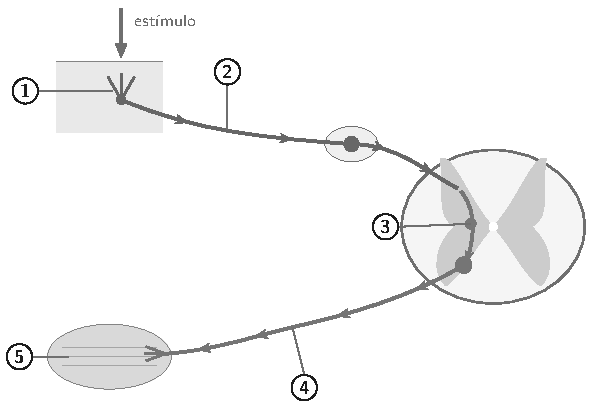
\includegraphics[max width=0.92\linewidth,max height=8.5cm]{bio/ner_arco_num}
\end{center}
\alts{2 y 4}{3 y 2}{3 y 4}{5 y 4}
\solucion{\textbf{Paso 1. ¿Qué nos piden?} El centro elaborador y la vía eferente.

\textbf{Paso 2. Sigue el camino del impulso.} 1: receptor en la piel. 2: neurona sensitiva, que lleva el impulso hacia la médula (vía aferente). 3: interneurona en la médula espinal (centro elaborador). 4: neurona motora, que lleva la orden desde la médula (vía eferente). 5: músculo (efector).

\textbf{Respuesta:} 3 y 4.

\textbf{¿Por qué no las otras?} El 2 es la vía aferente: lleva el impulso \textbf{hacia} el centro, no desde él. El 5 es el efector, el músculo que responde, no el centro elaborador.

\textbf{\color{cienciaD}Para recordar.} Aferente llega al centro; eferente sale del centro hacia el efector.}{C}
\end{elejemplo}
\motivacion{Cuidar tu sistema nervioso también es dormir bien y descansar. Estudia con constancia, no toda la noche antes.}

%% =====================================================================
%% bio_reproduccion
\section[Sistemas reproductores, gametos y fecundación]{Sistemas reproductores, gametos y fecundación}
\modcomun\ \ {\color{gris}\itshape Estructura y función de los sistemas reproductores femenino y masculino, cómo son el ovocito y el espermatozoide, dónde y cómo ocurre la fecundación, el camino del embrión hasta la implantación y las dimensiones de la sexualidad humana.\par}
\subsection{Sistema reproductor femenino}
El sistema reproductor femenino produce los \textbf{ovocitos} y las \textbf{hormonas sexuales}, recibe a los espermatozoides y alberga al embrión durante la gestación.

 
\begin{itemize}
  \item \textbf{Ovarios:} dos glándulas en la cavidad pelviana. Contienen los folículos, donde maduran los ovocitos, y producen \textbf{estrógeno} y \textbf{progesterona}.
  \item \textbf{Trompas uterinas (oviductos):} conductos que van de cada ovario al útero. Sus \textbf{fimbrias} captan el ovocito liberado. En su tercio externo (la ampolla) ocurre la \textbf{fecundación}.
  \item \textbf{Útero:} órgano hueco y muscular. Su pared tiene una capa muscular, el \textbf{miometrio}, que se contrae en el parto, y una capa interna, el \textbf{endometrio}, donde se implanta el embrión y que se desprende en cada menstruación.
  \item \textbf{Cuello uterino:} comunica el útero con la vagina. Produce el \textbf{moco cervical}, que cambia durante el ciclo.
  \item \textbf{Vagina:} conducto que recibe al pene en la relación sexual, por donde sale la menstruación y que forma parte del canal del parto. La \textbf{vulva} son los genitales externos.
\end{itemize}
  
\begin{center}
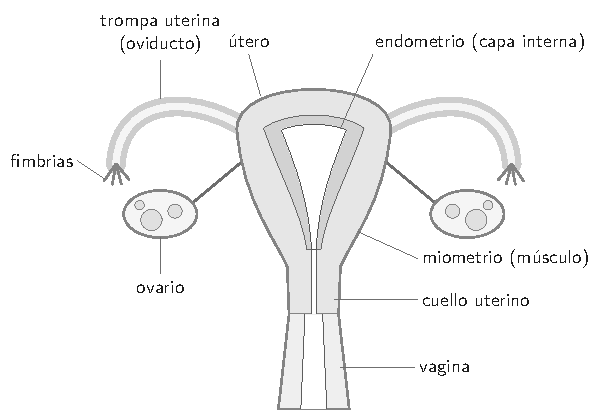
\includegraphics[max width=0.92\linewidth,max height=8.5cm]{bio/rep_femenino}
\end{center}
\subsection{Sistema reproductor masculino}
El sistema reproductor masculino produce los \textbf{espermatozoides} y la hormona \textbf{testosterona}, y los deposita en el sistema femenino.

 
\begin{itemize}
  \item \textbf{Testículos:} en los \textbf{túbulos seminíferos} se forman los espermatozoides (espermatogénesis), de manera continua desde la pubertad. Las \textbf{células de Leydig} producen testosterona.
  \item \textbf{Escroto:} bolsa de piel que aloja los testículos fuera del abdomen, a una temperatura unos 2 a 3 °C menor que la del cuerpo, necesaria para formar espermatozoides.
  \item \textbf{Epidídimo:} tubo enrollado sobre cada testículo. Allí los espermatozoides \textbf{maduran}, adquieren la capacidad de moverse y se almacenan.
  \item \textbf{Conductos deferentes:} llevan los espermatozoides desde el epidídimo hasta la uretra. Son los que se cortan en la vasectomía.
  \item \textbf{Glándulas anexas:} las \textbf{vesículas seminales} aportan un líquido con fructosa (energía); la \textbf{próstata}, un líquido que protege a los espermatozoides de la acidez vaginal; las \textbf{glándulas bulbouretrales}, un líquido que lubrica la uretra. Estos líquidos más los espermatozoides forman el \textbf{semen}.
  \item \textbf{Uretra y pene:} la uretra conduce el semen y también la orina, aunque nunca al mismo tiempo.
\end{itemize}
  
\begin{center}
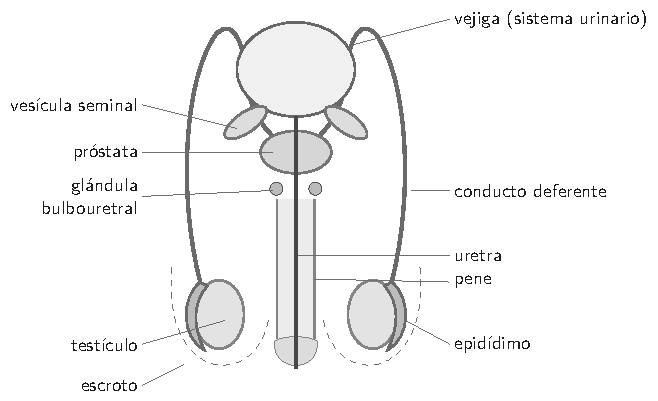
\includegraphics[max width=0.92\linewidth,max height=8.5cm]{bio/rep_masculino}
\end{center}
\subsection{Los gametos: ovocito y espermatozoide}
\begin{center}
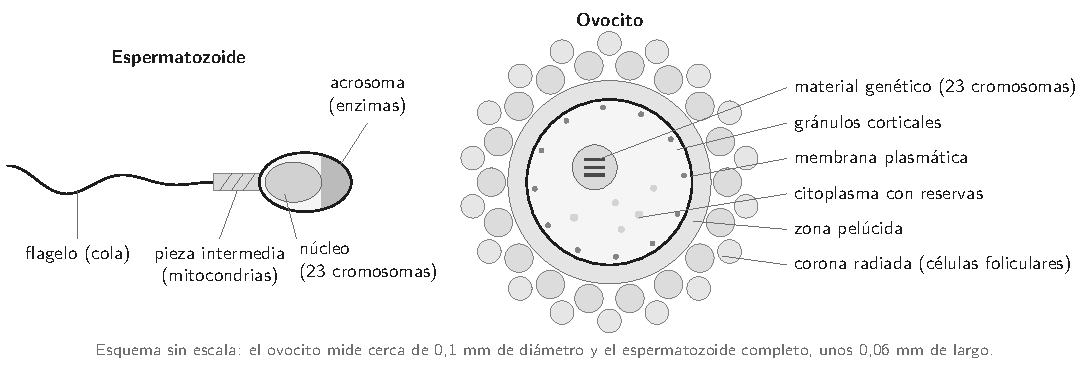
\includegraphics[max width=0.92\linewidth,max height=8.5cm]{bio/rep_gametos}
\end{center}
 
\begin{center}\small
\begin{tabularx}{\linewidth}{@{}>{\raggedright\arraybackslash\hsize=0.60\hsize}X>{\raggedright\arraybackslash\hsize=1.20\hsize}X>{\raggedright\arraybackslash\hsize=1.20\hsize}X@{}}
\toprule
 & \textbf{Espermatozoide} & \textbf{Ovocito} \\
\midrule
Dónde se forma & túbulos seminíferos del testículo & folículos del ovario \\
Cantidad & decenas o cientos de millones en cada eyaculación; se forman de manera continua desde la pubertad & en general uno por ciclo; su formación comienza antes del nacimiento \\
Tamaño y forma & muy pequeño (unos 0,06 mm), con cabeza, pieza intermedia y flagelo & una de las células más grandes del cuerpo (cerca de 0,1 mm), esférico \\
Movilidad & se mueve con su flagelo, gracias al ATP de las mitocondrias de la pieza intermedia & no se mueve por sí mismo; lo desplazan los cilios y las contracciones de la trompa \\
Qué aporta al cigoto & 23 cromosomas, entre ellos un X o un Y, que define el sexo cromosómico & 23 cromosomas (siempre un X), casi todo el citoplasma, las reservas y las mitocondrias \\
\bottomrule
\end{tabularx}
\end{center}
 
\begin{clave}[{Recuerda}] El \textbf{acrosoma} es una vesícula en la punta de la cabeza del espermatozoide. Contiene \textbf{enzimas} que digieren las cubiertas del ovocito (corona radiada y zona pelúcida). El ovocito que se libera en la ovulación está detenido en la segunda división de la meiosis y la termina solo si es fecundado.\end{clave}
\subsection{La fecundación}
La \textbf{fecundación} es la unión del espermatozoide con el ovocito. Ocurre normalmente en el \textbf{tercio externo de la trompa uterina}, poco después de la ovulación.

 

Tras la eyaculación, los espermatozoides recorren vagina, cuello uterino, útero y trompa. En el camino se \textbf{capacitan}: cambia su membrana y quedan listos para fecundar. Solo unos pocos cientos llegan cerca del ovocito.

 

\textbf{Etapas:}

 
\begin{enumerate}
  \item El espermatozoide atraviesa la \textbf{corona radiada}.
  \item Se une a la \textbf{zona pelúcida} y ocurre la \textbf{reacción acrosómica}: el acrosoma libera sus enzimas, que abren un camino a través de la zona pelúcida.
  \item Las \textbf{membranas} de ambos gametos se fusionan y el núcleo del espermatozoide entra al ovocito.
  \item \textbf{Reacción cortical:} los gránulos corticales liberan su contenido y la zona pelúcida cambia, de modo que no entran más espermatozoides (se evita la \textbf{polispermia}).
\end{enumerate}
 

El ovocito termina su meiosis, los dos núcleos (pronúcleos) se unen y se forma el \textbf{cigoto}, con 46 cromosomas: 23 de cada progenitor.

  
\begin{center}
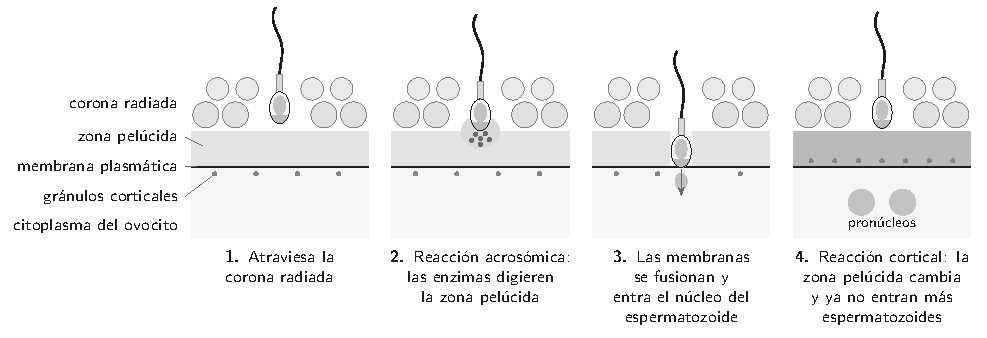
\includegraphics[max width=0.92\linewidth,max height=8.5cm]{bio/rep_fecundacion}
\end{center}
\subsection{Del cigoto a la implantación}
\begin{center}
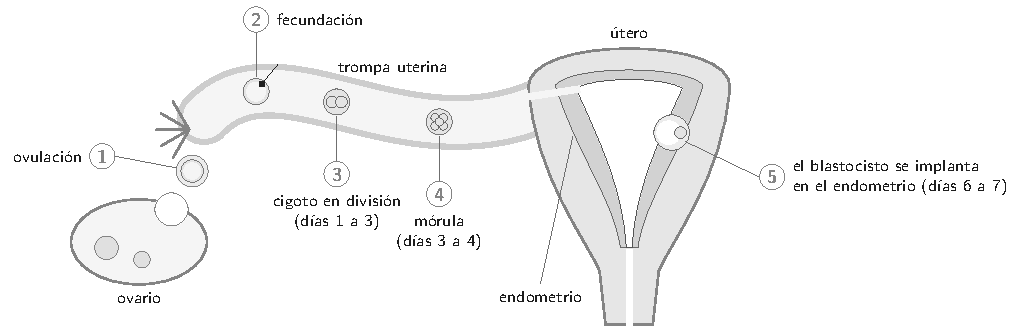
\includegraphics[max width=0.92\linewidth,max height=8.5cm]{bio/rep_trayecto}
\end{center}
  

Mientras viaja por la trompa hacia el útero, el cigoto se divide por mitosis (\textbf{segmentación}): 2, 4, 8 células\dots{} Hacia el día 3 o 4 es una esfera maciza de células, la \textbf{mórula}. Al llegar al útero se transforma en \textbf{blastocisto}, una esfera hueca.

 

Entre los días 6 y 7 después de la fecundación, el blastocisto se \textbf{implanta} (anida) en el \textbf{endometrio}. Sus células externas formarán parte de la \textbf{placenta} y empiezan a producir la hormona \textbf{hCG}, que es la que detectan las pruebas de embarazo.

  
\begin{clave}[{Recuerda}] · Fecundación: en la trompa uterina.\par · Implantación: en el endometrio del útero, unos 6 a 7 días después.\par · Si el embrión se implanta fuera del útero, por ejemplo en la trompa, se habla de embarazo \textbf{ectópico}, una urgencia médica.\par · La hCG se produce después de la implantación; por eso una prueba de embarazo hecha demasiado pronto puede salir negativa.\end{clave}
\subsection{Sexualidad humana}
La sexualidad es parte de la vida de todas las personas y va mucho más allá de la reproducción. Se suele describir con tres dimensiones que se relacionan entre sí:

 
\begin{itemize}
  \item \textbf{Biológica:} anatomía, hormonas, cambios de la pubertad, reproducción y salud sexual.
  \item \textbf{Psicológica y afectiva:} emociones, autoestima, identidad, vínculos, forma de vivir el afecto y la intimidad.
  \item \textbf{Social:} normas, cultura, valores, roles y la influencia de la familia, los pares y los medios.
\end{itemize}
 

Una sexualidad sana contribuye al \textbf{bienestar integral} de la persona y de sus relaciones.

  
\begin{clave}[{Claves para relaciones sanas}] · \textbf{Consentimiento:} libre, informado y entusiasta; se puede retirar en cualquier momento y se pide cada vez.\par · \textbf{Respeto:} a los tiempos, decisiones, límites y diversidad de cada persona.\par · \textbf{Cuidado:} de la propia salud y de la del otro (preservativo, exámenes de ITS, controles de salud).\par · \textbf{Responsabilidad:} tomar decisiones informadas y hacerse cargo de sus consecuencias.\par · \textbf{Comunicación:} conversar con confianza sobre lo que se siente, se quiere y no se quiere.\end{clave}
\subsection{Lo clave del tema}
\begin{center}\small
\begin{tabularx}{\linewidth}{@{}>{\raggedright\arraybackslash\hsize=0.64\hsize}X>{\raggedright\arraybackslash\hsize=1.36\hsize}X@{}}
\toprule
\textbf{Estructura} & \textbf{Función principal} \\
\midrule
Ovario & madura los ovocitos; produce estrógeno y progesterona \\
Trompa uterina & capta el ovocito; lugar de la fecundación; lleva el embrión al útero \\
Endometrio & lugar de implantación; se desprende en la menstruación \\
Testículo & forma espermatozoides (túbulos seminíferos) y testosterona (células de Leydig) \\
Epidídimo & maduración y almacenamiento; los espermatozoides adquieren movilidad \\
Conducto deferente & transporta espermatozoides hacia la uretra \\
Acrosoma & enzimas que digieren la corona radiada y la zona pelúcida \\
Pieza intermedia & mitocondrias que producen el ATP para el flagelo \\
Gránulos corticales & cambian la zona pelúcida y bloquean la polispermia \\
\bottomrule
\end{tabularx}
\end{center}
 
\begin{clave}[{Recuerda}] · Cada gameto tiene 23 cromosomas; el cigoto, 46.\par · El espermatozoide define el sexo cromosómico (lleva X o Y); el ovocito siempre lleva X.\par · El ovocito aporta casi todo el citoplasma y las mitocondrias del cigoto.\par · La fecundación ocurre en la trompa y la implantación, en el endometrio.\end{clave}
 
\begin{clave}[{Método PAES}] 1. Ubica la estructura o el proceso del que habla el enunciado (esquema numerado, gameto, etapa). 2. Recuerda su función. 3. Predice qué pasa si esa estructura falla: ¿qué paso de la reproducción se interrumpe y cuáles siguen igual? 4. En experimentos, compara cada grupo con el control y concluye solo lo que muestran los datos.\end{clave}
\begin{elejemplo}{PAES Regular 2026, adaptada}
Un espermiograma muestra que los espermatozoides de un paciente tienen forma normal y están en cantidad adecuada, pero casi no se desplazan. Al microscopio electrónico se observa que sus mitocondrias están alteradas. El siguiente esquema muestra las partes de un espermatozoide:

¿Qué estructura del esquema está alterada y qué función se ve afectada?
\begin{center}
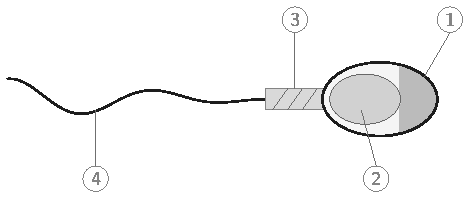
\includegraphics[max width=0.92\linewidth,max height=8.5cm]{bio/rep_esperm_num}
\end{center}
\altslargas{La estructura 1, que libera enzimas para atravesar las cubiertas del ovocito.}{La estructura 2, que aporta la información genética al cigoto.}{La estructura 3, que produce el ATP que mueve el flagelo.}{La estructura 4, que almacena las reservas de energía del espermatozoide.}
\solucion{\textbf{Paso 1. ¿Qué nos piden?} Relacionar un dato (mitocondrias alteradas y poco movimiento) con una parte del espermatozoide y su función.

\textbf{Paso 2. Identifica las partes.} 1 es el acrosoma, 2 el núcleo, 3 la pieza intermedia y 4 el flagelo.

\textbf{Paso 3. ¿Dónde están las mitocondrias?} En la \textbf{pieza intermedia}, enrolladas alrededor del inicio del flagelo. Producen el \textbf{ATP} que el flagelo usa para moverse. Si fallan, el flagelo existe pero no tiene energía: el espermatozoide casi no se desplaza.

\textbf{Respuesta:} la estructura 3, que produce el ATP que mueve el flagelo.

\textbf{¿Por qué no las otras?} El acrosoma (1) participa en la fecundación, no en el movimiento, y no tiene mitocondrias. El núcleo (2) lleva los cromosomas; su alteración no explica la falta de movimiento. El flagelo (4) es el que se mueve, pero no almacena reservas ni tiene mitocondrias: recibe la energía desde la pieza intermedia.

\textbf{\color{cienciaD}Para recordar.} Las mitocondrias de la pieza intermedia producen el ATP que mueve el flagelo.}{C}
\end{elejemplo}
\motivacion{Gametos, fecundación y sistemas reproductores: un tema largo y ya es tuyo. Te ganaste un descanso con ronroneo.}

%% =====================================================================
%% bio_ciclo
\section[Ciclo ovárico y ciclo uterino]{Ciclo ovárico y ciclo uterino}
\modcomun\ \ {\color{gris}\itshape Las fases del ciclo ovárico (folicular, ovulación y lútea) y del ciclo uterino (menstrual, proliferativa y secretora), las hormonas FSH, LH, estrógeno y progesterona, su regulación por el eje hipotálamo-hipófisis-ovario, la lectura de gráficos de 28 días y qué cambia si hay fecundación.\par}
\subsection{Dos ciclos que van juntos}
Desde la pubertad hasta la menopausia, el sistema reproductor femenino repite un ciclo que prepara, cada mes, un ovocito para ser fecundado y un endometrio para recibir al embrión. En realidad son \textbf{dos ciclos coordinados por hormonas}:

 
\begin{itemize}
  \item \textbf{Ciclo ovárico:} ocurre en el \textbf{ovario}. Madura un folículo, se libera un ovocito y se forma el cuerpo lúteo.
  \item \textbf{Ciclo uterino (o menstrual):} ocurre en el \textbf{endometrio}. Se desprende, crece y se prepara para la implantación.
\end{itemize}
 

Por convención, el \textbf{día 1} es el primer día de la menstruación. Un ciclo dura en promedio \textbf{28 días}, aunque es normal que dure entre unos 21 y 35 días y que varíe un poco de un mes a otro.

  
\begin{clave}[{Las cuatro hormonas del ciclo}] · \textbf{FSH} (hormona folículo estimulante), de la hipófisis: hace crecer los folículos.\par · \textbf{LH} (hormona luteinizante), de la hipófisis: su pico provoca la ovulación y forma el cuerpo lúteo.\par · \textbf{Estrógeno}, del folículo: engrosa el endometrio.\par · \textbf{Progesterona}, del cuerpo lúteo: prepara y mantiene el endometrio.\end{clave}
\subsection{El ciclo ovárico}
\begin{center}
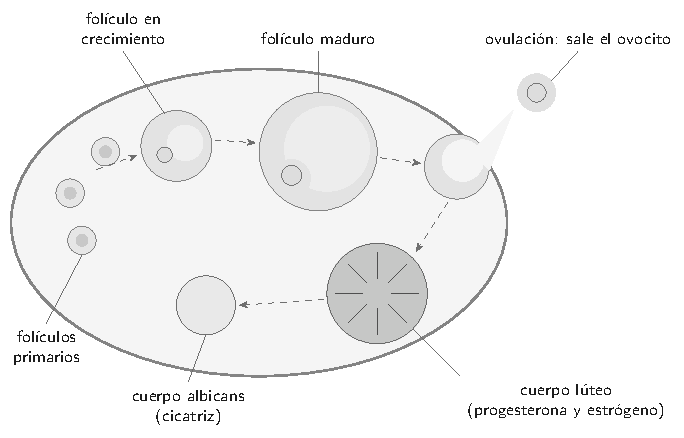
\includegraphics[max width=0.92\linewidth,max height=8.5cm]{bio/rep_ovario}
\end{center}
  

\textbf{Fase folicular} (días 1 a 13, aproximadamente). La \textbf{FSH} estimula el crecimiento de varios folículos; uno se vuelve dominante y llega a \textbf{folículo maduro}. Sus células producen cada vez más \textbf{estrógeno}.

 

\textbf{Ovulación} (cerca del día 14). Un \textbf{pico de LH} hace que el folículo maduro se rompa y libere el ovocito, que es captado por la trompa.

  

\textbf{Fase lútea} (días 15 a 28). Por acción de la LH, el folículo roto se transforma en \textbf{cuerpo lúteo}, que secreta \textbf{progesterona} y algo de estrógeno. Si no hay fecundación, el cuerpo lúteo dura unos 10 a 14 días y degenera en una cicatriz (cuerpo albicans).

 
\begin{clave}[{Recuerda}] La fase lútea dura casi siempre unos 14 días. Lo que cambia entre ciclos largos y cortos es la fase folicular. Por eso la ovulación ocurre unos \textbf{14 días antes} de la siguiente menstruación: en un ciclo de 32 días, cerca del día 18.\end{clave}
\subsection{El ciclo uterino}
\begin{itemize}
  \item \textbf{Fase menstrual} (días 1 a 5, aproximadamente): al caer la progesterona y el estrógeno, la capa superficial del endometrio se desprende y sale con sangre: es la \textbf{menstruación}.
  \item \textbf{Fase proliferativa} (días 6 a 14): el \textbf{estrógeno} del folículo hace que el endometrio se regenere y se engrose.
  \item \textbf{Fase secretora} (días 15 a 28): la \textbf{progesterona} del cuerpo lúteo hace que el endometrio se llene de glándulas y vasos sanguíneos, quede más grueso y secrete nutrientes. Está listo para recibir un embrión.
\end{itemize}
 
\begin{center}\small
\begin{tabularx}{\linewidth}{@{}>{\raggedright\arraybackslash\hsize=1.23\hsize}X>{\raggedright\arraybackslash\hsize=0.82\hsize}X>{\raggedright\arraybackslash\hsize=0.95\hsize}X@{}}
\toprule
\textbf{Ciclo ovárico} & \textbf{Ciclo uterino} & \textbf{Hormona que manda} \\
\midrule
inicio de la fase folicular & fase menstrual & caída de progesterona \\
fase folicular & fase proliferativa & estrógeno \\
fase lútea & fase secretora & progesterona \\
\bottomrule
\end{tabularx}
\end{center}
  
\begin{center}
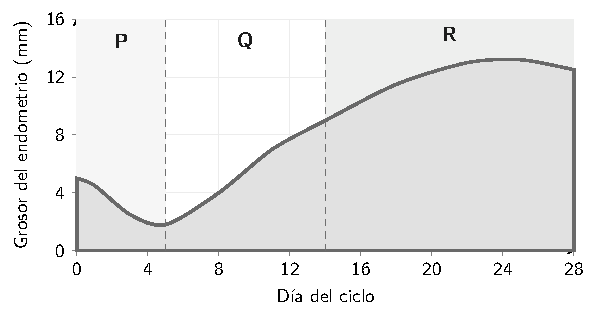
\includegraphics[max width=0.92\linewidth,max height=8.5cm]{bio/rep_endometrio}
\end{center}
 
\begin{clave}[{Recuerda}] P es la fase menstrual, Q la proliferativa (estrógeno) y R la secretora (progesterona).\end{clave}
\subsection{Quién regula a quién}
El ciclo se controla con un \textbf{eje hormonal}:

 
\begin{enumerate}
  \item El \textbf{hipotálamo} libera \textbf{GnRH}.
  \item La GnRH estimula a la \textbf{hipófisis anterior}, que libera \textbf{FSH} y \textbf{LH}.
  \item FSH y LH actúan sobre el \textbf{ovario}, que produce \textbf{estrógeno} y \textbf{progesterona}.
  \item Estas hormonas actúan sobre el \textbf{endometrio} y, además, vuelven al hipotálamo y a la hipófisis.
\end{enumerate}
 

\textbf{Retroalimentación negativa:} cuando el estrógeno y la progesterona están altos, frenan la liberación de GnRH, FSH y LH. Por eso en la fase lútea no maduran nuevos folículos, y por eso funcionan las píldoras anticonceptivas.

 

\textbf{Retroalimentación positiva:} a mitad del ciclo, un nivel alto y sostenido de estrógeno hace lo contrario: provoca el \textbf{pico de LH} que desencadena la ovulación.

  
\begin{center}
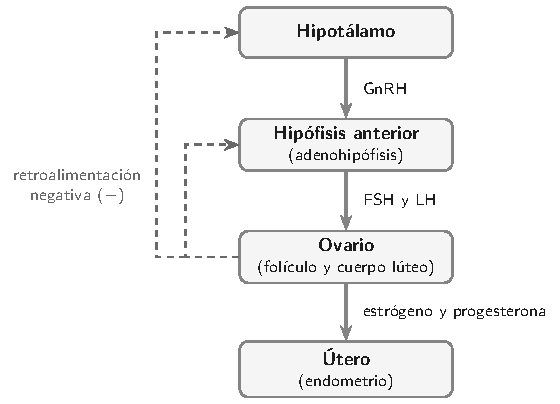
\includegraphics[max width=0.92\linewidth,max height=8.5cm]{bio/rep_eje}
\end{center}
 
\begin{clave}[{Recuerda}] Si el ovario deja de producir hormonas (por ejemplo, en la menopausia), desaparece el freno y la FSH y la LH \textbf{suben}.\end{clave}
\subsection{Leer el gráfico completo}
\begin{center}
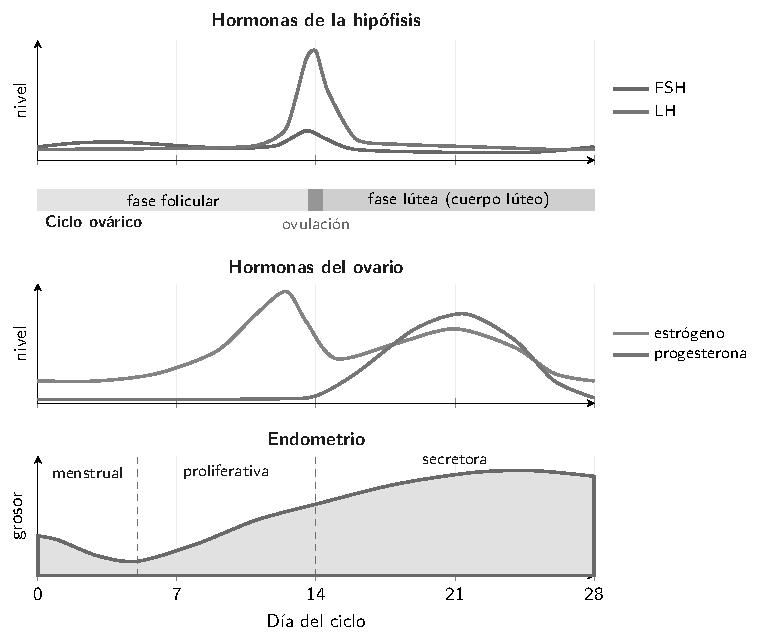
\includegraphics[max width=0.92\linewidth,max height=8.5cm]{bio/rep_ciclo_hormonas}
\end{center}
  

Para leer un gráfico del ciclo, recorre los días de izquierda a derecha y pregúntate qué hormona sube y qué efecto tiene:

 
\begin{itemize}
  \item \textbf{Días 1 a 5:} hormonas ováricas bajas; el endometrio se desprende.
  \item \textbf{Días 6 a 13:} la FSH hace crecer el folículo; el estrógeno sube y engrosa el endometrio.
  \item \textbf{Día 14:} el estrógeno alto provoca el pico de LH; ocurre la ovulación.
  \item \textbf{Días 15 a 25:} el cuerpo lúteo produce progesterona; el endometrio está en fase secretora.
  \item \textbf{Días 25 a 28:} si no hubo embarazo, el cuerpo lúteo degenera, la progesterona cae y comienza una nueva menstruación.
\end{itemize}
 
\begin{clave}[{Pistas rápidas}] Un pico agudo y breve a mitad del ciclo es la LH. La hormona que solo sube después de la ovulación es la progesterona. La que tiene dos subidas, una antes y otra después de la ovulación, es el estrógeno.\end{clave}
\subsection{¿Y si hay fecundación?}
\textbf{Sin fecundación:} el cuerpo lúteo degenera al final del ciclo, la progesterona y el estrógeno caen, el endometrio se desprende (menstruación) y, sin el freno hormonal, la FSH vuelve a subir para iniciar otro ciclo.

 

\textbf{Con fecundación:} el embrión se implanta y produce \textbf{hCG}. La hCG mantiene vivo el \textbf{cuerpo lúteo}, que sigue secretando progesterona. Así el endometrio se mantiene, \textbf{no hay menstruación} y no maduran nuevos folículos. Desde el segundo o tercer mes, la \textbf{placenta} asume la producción de progesterona.

  
\begin{center}
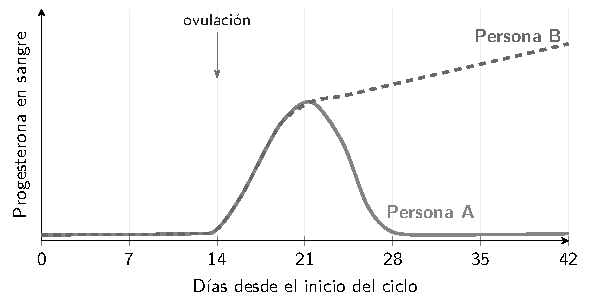
\includegraphics[max width=0.92\linewidth,max height=8.5cm]{bio/rep_embarazo}
\end{center}
 
\begin{clave}[{Recuerda}] En el gráfico, la persona B está embarazada: la hCG mantiene el cuerpo lúteo y la progesterona sigue alta.\end{clave}
\subsection{Lo clave del tema}
\begin{center}\small
\begin{tabularx}{\linewidth}{@{}>{\raggedright\arraybackslash\hsize=0.52\hsize}X>{\raggedright\arraybackslash\hsize=1.15\hsize}X>{\raggedright\arraybackslash\hsize=1.39\hsize}X>{\raggedright\arraybackslash\hsize=0.94\hsize}X@{}}
\toprule
\textbf{Hormona} & \textbf{La produce} & \textbf{Efecto principal} & \textbf{Cuándo está alta} \\
\midrule
GnRH & hipotálamo & estimula la liberación de FSH y LH & todo el ciclo, en pulsos \\
FSH & hipófisis anterior & crecimiento de los folículos & inicio de la fase folicular \\
LH & hipófisis anterior & ovulación y formación del cuerpo lúteo & pico cerca del día 14 \\
Estrógeno & folículo (y cuerpo lúteo) & engrosa el endometrio (fase proliferativa) & antes de la ovulación \\
Progesterona & cuerpo lúteo (luego, la placenta) & prepara y mantiene el endometrio (fase secretora) & fase lútea \\
hCG & embrión implantado & mantiene el cuerpo lúteo & inicio del embarazo \\
\bottomrule
\end{tabularx}
\end{center}
 
\begin{clave}[{Recuerda}] · El pico de LH provoca la ovulación.\par · La caída de progesterona provoca la menstruación.\par · La ovulación ocurre unos 14 días antes de la siguiente menstruación.\par · Estrógeno y progesterona altos frenan la FSH y la LH; si bajan, la FSH y la LH suben.\end{clave}
 
\begin{clave}[{Método PAES}] 1. Ubica el día o la fase del ciclo de la que habla la pregunta. 2. Identifica qué estructura está activa (folículo o cuerpo lúteo) y qué hormona produce. 3. Sigue la cadena: hipotálamo \ensuremath{\rightarrow} hipófisis \ensuremath{\rightarrow} ovario \ensuremath{\rightarrow} endometrio, y recuerda que las hormonas del ovario frenan a las de arriba. 4. Si cambia la duración del ciclo, cuenta 14 días hacia atrás desde la siguiente menstruación.\end{clave}
\begin{elejemplo}{PAES Regular 2026, adaptada}
En una clase de biología se presenta el siguiente gráfico con la concentración en sangre de dos hormonas producidas por el ovario a lo largo de un ciclo de 28 días sin embarazo:

¿Qué hormona es Y y qué estructura del ovario la produce principalmente?
\begin{center}
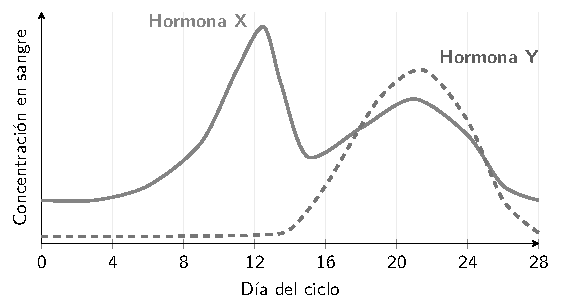
\includegraphics[max width=0.92\linewidth,max height=8.5cm]{bio/rep_ciclo_xy}
\end{center}
\altslargas{Estrógeno, producido por el folículo en crecimiento.}{Progesterona, producida por el cuerpo lúteo.}{LH, producida por la hipófisis.}{Progesterona, producida por el folículo maduro antes de la ovulación.}
\solucion{\textbf{Paso 1. ¿Qué nos piden?} Identificar la hormona Y por la forma de su curva y decir qué estructura la produce.

\textbf{Paso 2. Lee la curva Y.} Está baja durante toda la primera mitad del ciclo, sube \textbf{solo después del día 14}, llega a su máximo cerca del día 21 y cae al final.

\textbf{Paso 3. Relaciona con el ovario.} Después de la ovulación, el folículo roto se transforma en \textbf{cuerpo lúteo}, que secreta progesterona. Cuando el cuerpo lúteo degenera (si no hay embarazo), la progesterona cae. Esa es exactamente la forma de Y.

\textbf{Respuesta:} Y es progesterona, producida por el cuerpo lúteo.

\textbf{¿Por qué no las otras?} El estrógeno es X: sube antes de la ovulación, producido por el folículo en crecimiento. La LH no la produce el ovario y su curva es un pico agudo y breve cerca del día 14. Antes de la ovulación todavía no existe el cuerpo lúteo y la progesterona está baja.

\textbf{\color{cienciaD}Para recordar.} La hormona que solo sube después de la ovulación es la progesterona del cuerpo lúteo.}{B}
\end{elejemplo}
\motivacion{FSH, LH, estrógeno y progesterona: ordenar el ciclo hormonal pide precisión, y tú la tienes.}

%% =====================================================================
%% bio_natalidad
\section[Control de la natalidad e ITS]{Control de la natalidad e ITS}
\modcomun\ \ {\color{gris}\itshape Cómo actúan los métodos naturales (Billings, calendario y temperatura basal), los artificiales reversibles (hormonales y de barrera) y los quirúrgicos (vasectomía y ligadura), cuál protege de las ITS, y las características del VIH, el herpes, la gonorrea y la clamidia.\par}
\subsection{Los métodos y cómo se clasifican}
\begin{center}
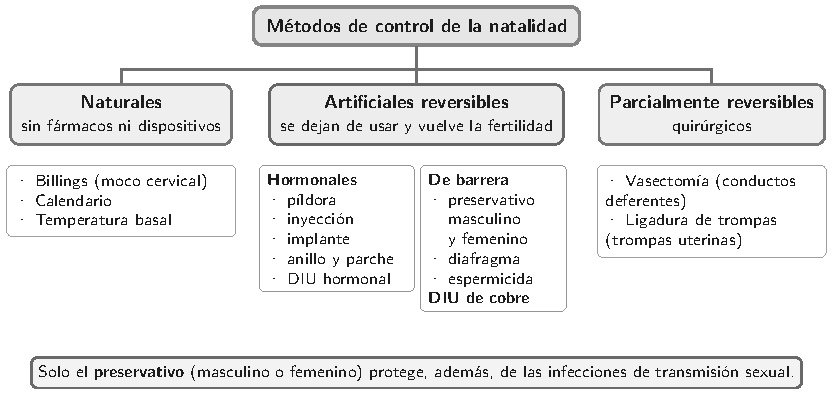
\includegraphics[max width=0.92\linewidth,max height=8.5cm]{bio/rep_metodos}
\end{center}
  

Los métodos de control de la natalidad permiten decidir si tener hijos y cuándo. Todos actúan sobre algún paso de la reproducción:

 
\begin{itemize}
  \item \textbf{impedir la ovulación} (hormonales);
  \item \textbf{impedir que los gametos se encuentren} (barrera, DIU de cobre, quirúrgicos, naturales);
  \item \textbf{dificultar la implantación} o el paso de espermatozoides por el moco cervical (efecto adicional de algunos hormonales).
\end{itemize}
  
\begin{clave}[{Recuerda}] · La \textbf{eficacia} depende del método y también de usarlo bien y siempre.\par · El único método que, además de prevenir el embarazo, protege de las ITS es el \textbf{preservativo}. Por eso se recomienda usarlo siempre, incluso junto a otro método (doble protección).\par · Elegir un método es una decisión informada y compartida, idealmente con orientación de un profesional de la salud.\end{clave}
\subsection{Métodos naturales}
Se basan en reconocer los \textbf{días fértiles} del ciclo y evitar las relaciones sexuales con penetración en esos días. Recuerda que los espermatozoides pueden vivir hasta unos 5 días en el sistema femenino y el ovocito, cerca de un día: los días fértiles van desde unos 5 días antes de la ovulación hasta el día siguiente a ella.

 
\begin{itemize}
  \item \textbf{Billings (moco cervical):} cerca de la ovulación el moco es abundante, transparente y elástico, como clara de huevo. Después se vuelve escaso y espeso.
  \item \textbf{Calendario (Ogino-Knaus):} se registran varios ciclos y se calcula cuándo ocurre la ovulación (unos 14 días antes de la siguiente menstruación).
  \item \textbf{Temperatura basal:} se mide al despertar, antes de levantarse. Después de la ovulación sube entre 0,3 y 0,5 °C por la progesterona y se mantiene alta hasta la menstruación.
\end{itemize}
  
\begin{center}
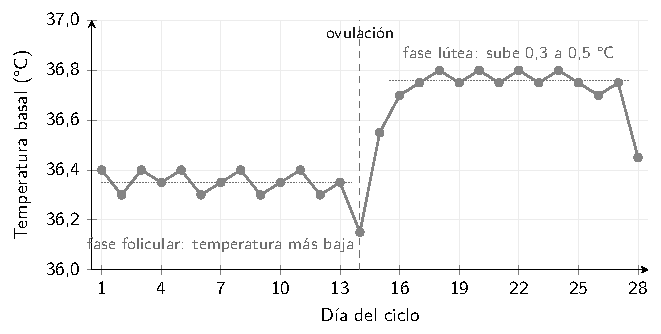
\includegraphics[max width=0.92\linewidth,max height=8.5cm]{bio/rep_temp_basal}
\end{center}
 
\begin{clave}[{Recuerda}] Son métodos de baja eficacia en el uso real, funcionan mejor con ciclos regulares y no protegen de las ITS. El alza de temperatura confirma que la ovulación \textbf{ya ocurrió}; no la anuncia antes.\end{clave}
\subsection{Métodos hormonales}
Contienen hormonas sintéticas parecidas al estrógeno y a la progesterona (progestinas): \textbf{píldora}, \textbf{inyección}, \textbf{implante subdérmico}, \textbf{anillo vaginal}, \textbf{parche} y \textbf{DIU hormonal}.

 

\textbf{Cómo actúan:}

 
\begin{enumerate}
  \item Mantienen altas estas hormonas y, por \textbf{retroalimentación negativa}, frenan la FSH y la LH: no madura un folículo y no hay pico de LH, así que \textbf{no hay ovulación}.
  \item Espesan el \textbf{moco cervical}, lo que dificulta el paso de los espermatozoides.
  \item Modifican el endometrio.
\end{enumerate}
 

Son muy eficaces y reversibles: al dejarlos, la fertilidad vuelve. Requieren indicación y control de salud.

  
\begin{clave}[{Anticoncepción de emergencia}] Es una dosis de hormona que se toma lo antes posible después de una relación sin protección (idealmente dentro de 72 horas). Retrasa o impide la ovulación. No interrumpe un embarazo ya implantado y no reemplaza a un método regular.\end{clave}
 
\begin{clave}[{Recuerda}] Ningún método hormonal protege de las ITS.\end{clave}
\subsection{Métodos de barrera y DIU}
\begin{itemize}
  \item \textbf{Preservativo masculino (condón):} funda de látex u otro material que se coloca sobre el pene erecto. Retiene el semen. Protege del embarazo y de las ITS.
  \item \textbf{Preservativo femenino:} funda que se coloca dentro de la vagina. También protege de las ITS.
  \item \textbf{Diafragma:} copa flexible que cubre el cuello uterino; se usa con espermicida.
  \item \textbf{Espermicida:} sustancia química que inmoviliza o destruye a los espermatozoides.
  \item \textbf{DIU de cobre:} dispositivo que se coloca dentro del útero; el cobre es tóxico para los espermatozoides e impide la fecundación. Dura varios años y se retira cuando se desea.
\end{itemize}
  
\begin{clave}[{Para usar bien el preservativo}] · Revisar la fecha de vencimiento y que el envase esté intacto.\par · Ponerlo desde el inicio de la relación, no solo antes de eyacular.\par · Usar uno nuevo en cada relación y solo uno a la vez.\par · Con lubricante, usar uno a base de agua si es de látex.\end{clave}
\subsection{Métodos quirúrgicos}
\begin{center}
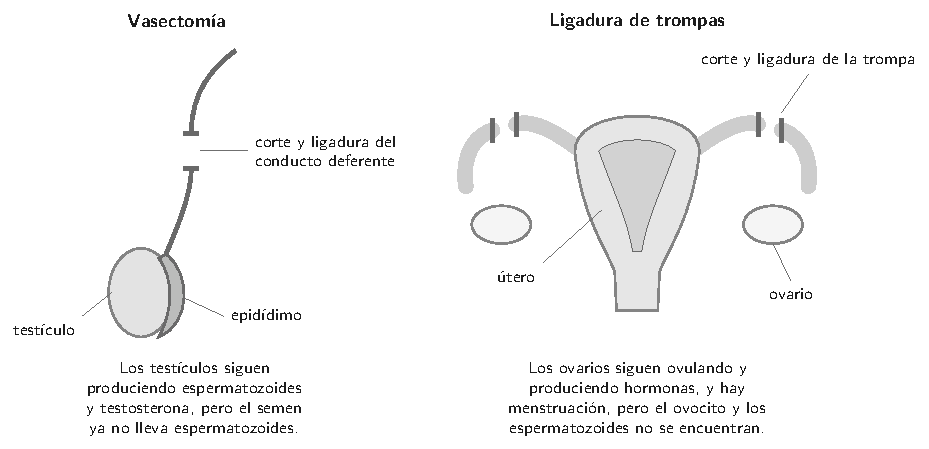
\includegraphics[max width=0.92\linewidth,max height=8.5cm]{bio/rep_quirurgicos}
\end{center}
  

\textbf{Vasectomía:} se cortan y ligan los \textbf{conductos deferentes}. Los testículos siguen produciendo espermatozoides (que el cuerpo reabsorbe) y testosterona; la erección y la eyaculación no cambian, pero el semen ya no lleva espermatozoides. No es inmediata: hay que esperar unos meses y confirmarlo con un examen de semen.

  

\textbf{Ligadura de trompas:} se cortan, ligan o bloquean las \textbf{trompas uterinas}. Los ovarios siguen ovulando y produciendo hormonas, y la menstruación continúa, pero el ovocito y los espermatozoides no se encuentran.

 
\begin{clave}[{Recuerda}] Se consideran \textbf{definitivos}. Se clasifican como parcialmente reversibles porque una cirugía puede reconectar los conductos, pero no siempre se recupera la fertilidad. No protegen de las ITS.\end{clave}
\subsection{Infecciones de transmisión sexual (ITS)}
\begin{center}\small
\begin{tabularx}{\linewidth}{@{}>{\raggedright\arraybackslash\hsize=0.42\hsize}X>{\raggedright\arraybackslash\hsize=0.96\hsize}X>{\raggedright\arraybackslash\hsize=1.20\hsize}X>{\raggedright\arraybackslash\hsize=1.20\hsize}X>{\raggedright\arraybackslash\hsize=1.20\hsize}X@{}}
\toprule
\textbf{ITS} & \textbf{Agente} & \textbf{Transmisión} & \textbf{Síntomas generales} & \textbf{Tratamiento} \\
\midrule
VIH / sida & virus (retrovirus) & relaciones sexuales, sangre (jeringas compartidas), de madre a hijo en el embarazo, parto o lactancia & puede pasar años sin síntomas; destruye linfocitos T CD4 y debilita el sistema inmune; el sida es su etapa avanzada, con infecciones oportunistas & antirretrovirales: no curan, pero controlan el virus; con carga viral indetectable no se transmite por vía sexual \\
Herpes genital & virus (VHS-2 y también VHS-1) & contacto de piel o mucosas con la zona infectada & vesículas y úlceras dolorosas que reaparecen; el virus queda latente en el cuerpo & antivirales que reducen los brotes; no hay cura \\
Gonorrea & bacteria (\emph{Neisseria gonorrhoeae}) & relaciones sexuales & secreción con pus y ardor al orinar; a menudo sin síntomas, sobre todo en mujeres; puede causar infertilidad & antibióticos \\
Clamidia & bacteria (\emph{Chlamydia trachomatis}) & relaciones sexuales & con frecuencia sin síntomas; secreción o dolor; si no se trata, daña las trompas y puede causar infertilidad & antibióticos \\
\bottomrule
\end{tabularx}
\end{center}
 
\begin{clave}[{Prevención}] Usar preservativo en todas las relaciones, hacerse exámenes periódicos (muchas ITS no dan síntomas), conversar con la pareja, no compartir jeringas y consultar ante cualquier síntoma. Las ITS bacterianas se curan con antibióticos; las virales no responden a antibióticos.\end{clave}
\subsection{Lo clave del tema}
\begin{center}\small
\begin{tabularx}{\linewidth}{@{}>{\raggedright\arraybackslash\hsize=1.21\hsize}X>{\raggedright\arraybackslash\hsize=1.21\hsize}X>{\raggedright\arraybackslash\hsize=1.09\hsize}X>{\raggedright\arraybackslash\hsize=0.48\hsize}X@{}}
\toprule
\textbf{Método} & \textbf{Cómo actúa} & \textbf{Clasificación} & \textbf{¿Protege de ITS?} \\
\midrule
Billings, calendario, temperatura basal & evitar las relaciones en los días fértiles & natural & no \\
Píldora, inyección, implante, anillo, parche & impiden la ovulación (frenan FSH y LH) y espesan el moco & artificial reversible (hormonal) & no \\
Preservativo masculino y femenino & retiene el semen: los gametos no se encuentran & artificial reversible (barrera) & \textbf{sí} \\
Diafragma y espermicida & barrera en el cuello uterino; inmoviliza espermatozoides & artificial reversible (barrera) & no \\
DIU de cobre & el cobre afecta a los espermatozoides & artificial reversible & no \\
Vasectomía y ligadura & cortan los conductos deferentes o las trompas & parcialmente reversible (quirúrgico) & no \\
\bottomrule
\end{tabularx}
\end{center}
 
\begin{clave}[{Recuerda}] · VIH y herpes son virus; gonorrea y clamidia, bacterias.\par · Muchas ITS no dan síntomas: el examen es la única forma de saberlo.\par · La vasectomía y la ligadura no cambian las hormonas ni la menstruación.\end{clave}
 
\begin{clave}[{Método PAES}] 1. Ubica qué paso de la reproducción bloquea el método (ovulación, encuentro de los gametos o implantación). 2. Para ITS, identifica el agente: bacteria (antibióticos) o virus (antivirales). 3. En tablas y gráficos, compara por grupos y concluye solo lo que muestran los datos. 4. En preguntas de investigación, busca qué se mide y qué se compara.\end{clave}
\begin{elejemplo}{Estilo PAES}
Una persona registra cada mañana, al despertar, su temperatura basal durante un ciclo de 28 días. Obtiene el siguiente gráfico:

¿Qué indica el alza sostenida de la temperatura desde el día 15?
\begin{center}
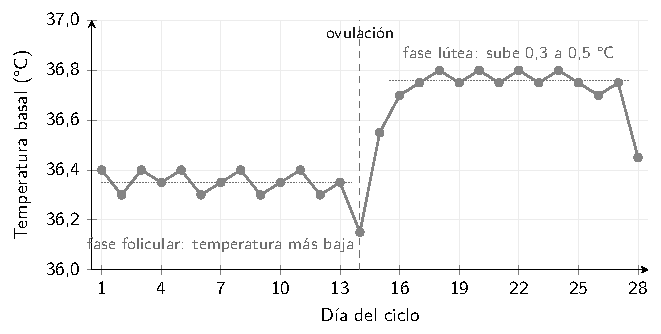
\includegraphics[max width=0.92\linewidth,max height=8.5cm]{bio/rep_temp_basal}
\end{center}
\altslargas{Que la ovulación ocurrirá en los próximos días.}{Que comenzó la menstruación.}{Que la persona tiene una infección.}{Que la ovulación ya ocurrió y el cuerpo lúteo está secretando progesterona.}
\solucion{\textbf{Paso 1. ¿Qué nos piden?} Interpretar el cambio de temperatura en la segunda mitad del ciclo.

\textbf{Paso 2. Recuerda la causa.} Después de la ovulación se forma el cuerpo lúteo, que secreta progesterona. La progesterona sube la temperatura basal entre 0,3 y 0,5 °C, y se mantiene alta mientras el cuerpo lúteo funciona.

\textbf{Paso 3. Lee el gráfico.} La temperatura se mantiene baja hasta el día 14 y sube desde el día 15 hasta casi el final: la ovulación ocurrió cerca del día 14.

\textbf{Respuesta:} que la ovulación ya ocurrió y el cuerpo lúteo está secretando progesterona.

\textbf{¿Por qué no las otras?} El alza aparece \textbf{después} de la ovulación, no antes: por eso este método confirma la ovulación, pero no la anticipa. La menstruación ocurre cuando la progesterona baja, y en el gráfico corresponde a la caída del día 28. Una fiebre por infección no forma este patrón de dos niveles que se repite en cada ciclo.

\textbf{\color{cienciaD}Para recordar.} El alza de la temperatura basal confirma que la ovulación ya ocurrió (efecto de la progesterona).}{D}
\end{elejemplo}
\motivacion{Conocer los métodos anticonceptivos y las ITS es cuidar tu salud y la de los demás. Este tema sirve para la prueba y para la vida.}

\chapter{Herencia y evolución}
%% =====================================================================
%% bio_ciclo_celular
\section[Cromatina y ciclo celular]{Cromatina y ciclo celular}
\modcomun\ \ {\color{gris}\itshape Cómo se empaqueta el ADN (nucleosomas, fibra, cromosoma, cromátidas hermanas y centrómero), las etapas del ciclo celular (G1, S, G2 y fase M), sus puntos de control y el cáncer como pérdida de control.\par}
\subsection{La cromatina y sus grados de compactación}
Una célula humana tiene cerca de \textbf{2 metros} de ADN dentro de un núcleo de unos 6 micrómetros. Cabe porque el ADN no está suelto: se enrolla en proteínas llamadas \textbf{histonas}. El conjunto de ADN e histonas es la \textbf{cromatina}.

 

La cromatina tiene varios \textbf{grados de compactación}:

 
\begin{itemize}
  \item \textbf{Nucleosoma:} un tramo de ADN da casi dos vueltas alrededor de un grupo de ocho histonas. Una hilera de nucleosomas parece un «collar de perlas».
  \item \textbf{Fibra de cromatina:} los nucleosomas se pliegan y se acercan entre sí.
  \item \textbf{Cromosoma:} la fibra forma bucles y se pliega más. Al dividirse la célula alcanza su \textbf{máxima compactación} y se ve al microscopio.
\end{itemize}
  
\begin{clave}[{¿Por qué cambia la compactación?}] En la interfase la cromatina está más \textbf{descondensada}: así las enzimas pueden leer los genes y replicar el ADN. Al dividirse, la cromatina se \textbf{condensa} al máximo: así los cromosomas se reparten entre las células hijas sin enredarse ni cortarse.\end{clave}
 
\begin{clave}[{Recuerda}] Cromatina y cromosoma son el mismo material (ADN con histonas) en distinto grado de compactación.\end{clave}
  
\begin{center}
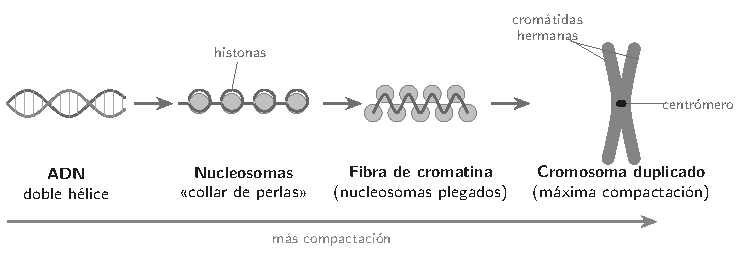
\includegraphics[max width=0.92\linewidth,max height=8.5cm]{bio/div_compactacion}
\end{center}
\subsection{Cromosomas, cromátidas y centrómero}
Antes de dividirse, la célula \textbf{copia su ADN}. Desde ese momento cada cromosoma tiene dos \textbf{cromátidas hermanas}: dos moléculas de ADN idénticas, unidas por el \textbf{centrómero}. Es un cromosoma \textbf{duplicado}.

 

Cuando las cromátidas hermanas se separan, cada una pasa a ser un cromosoma \textbf{simple} (de una cromátida).

 

\textbf{Cromosomas homólogos.} Las células del cuerpo son \textbf{diploides (2n)}: tienen pares de cromosomas, uno heredado de la madre y otro del padre. Los dos cromosomas de un par son \textbf{homólogos}: llevan los mismos genes en el mismo orden, pero pueden tener versiones distintas (alelos). En el ser humano, 2n = 46: 23 pares.

  
\begin{clave}[{Cómo contar}] · Número de \textbf{cromosomas} = número de \textbf{centrómeros}.\par · Cada cromosoma duplicado aporta \textbf{dos cromátidas} (dos moléculas de ADN).\par · Cada cromosoma simple aporta \textbf{una cromátida}.\end{clave}
 
\begin{center}\small
\begin{tabular}{@{}lll@{}}
\toprule
\textbf{Célula humana} & \textbf{Cromosomas} & \textbf{Cromátidas} \\
\midrule
En G1 (antes de replicar) & 46 & 46 \\
En G2 (después de replicar) & 46 & 92 \\
\bottomrule
\end{tabular}
\end{center}
 
\begin{clave}[{Recuerda}] Las cromátidas hermanas son \textbf{copias idénticas} que vienen de la replicación. Los homólogos son \textbf{dos cromosomas distintos}, uno de cada progenitor.\end{clave}
\subsection{Las etapas del ciclo celular}
El \textbf{ciclo celular} es la secuencia de etapas que vive una célula desde que se forma hasta que se divide en dos. Tiene dos grandes partes:

 

\textbf{Interfase} (la más larga, en muchas células más del 90 \% del ciclo):

 
\begin{itemize}
  \item \textbf{G1:} la célula crece, fabrica proteínas y organelos y cumple su función.
  \item \textbf{S:} síntesis (replicación) del ADN. Cada cromosoma queda con dos cromátidas.
  \item \textbf{G2:} la célula sigue creciendo y se prepara para dividirse.
\end{itemize}
 

\textbf{Fase M:} la \textbf{mitosis} (reparto del núcleo) y la \textbf{citocinesis} (reparto del citoplasma).

 

Algunas células salen del ciclo desde G1 a un estado de reposo llamado \textbf{G0}: siguen vivas y funcionando, pero no se dividen. Ejemplos: la mayoría de las neuronas y las células del músculo cardíaco.

  
\begin{center}
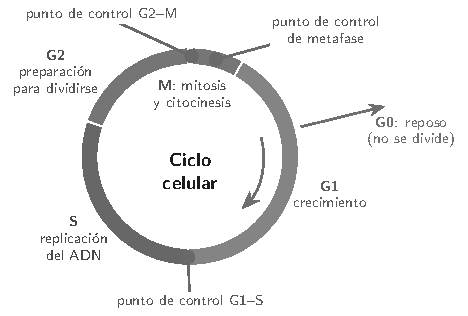
\includegraphics[max width=0.92\linewidth,max height=8.5cm]{bio/div_ciclo}
\end{center}
\subsection{Los puntos de control}
El ciclo no avanza «a ciegas». En ciertos momentos, proteínas de control revisan si todo está en orden. Si algo falla, el ciclo \textbf{se detiene} hasta que se corrige; si el daño no tiene arreglo, la célula activa la \textbf{apoptosis} (muerte celular programada).

 
\begin{center}\small
\begin{tabularx}{\linewidth}{@{}>{\raggedright\arraybackslash\hsize=0.57\hsize}X>{\raggedright\arraybackslash\hsize=1.43\hsize}X@{}}
\toprule
\textbf{Punto de control} & \textbf{Qué revisa} \\
\midrule
G1--S & tamaño celular, nutrientes, señales para dividirse y ADN sin daño, antes de replicarlo \\
G2--M & ADN replicado por completo y sin daño, antes de entrar en mitosis \\
Metafase & todos los cromosomas unidos al huso mitótico, antes de separar las cromátidas \\
\bottomrule
\end{tabularx}
\end{center}
  
\begin{ejemplo}[{Ejemplo resuelto}] Se trata un cultivo con un fármaco que impide armar el huso mitótico. Los cromosomas no logran unirse al huso, así que el punto de control de metafase no deja pasar a la anafase: las células se \textbf{acumulan en metafase}. Así actúan algunos fármacos contra el cáncer y así se preparan las células para fotografiar cromosomas.\end{ejemplo}
 
\begin{clave}[{Recuerda}] Cada punto de control revisa lo que acaba de pasar y deja avanzar solo si está bien: antes de replicar (G1--S), antes de dividir (G2--M) y antes de separar (metafase).\end{clave}
\subsection{Cáncer: cuando se pierde el control}
Los puntos de control dependen de genes. Hay dos grupos importantes:

 
\begin{itemize}
  \item \textbf{Protooncogenes:} codifican proteínas que estimulan la división, como un acelerador. Si mutan y quedan siempre activos (\textbf{oncogenes}), la célula recibe la orden de dividirse sin parar.
  \item \textbf{Genes supresores de tumores:} codifican proteínas que frenan el ciclo o activan la apoptosis, como el freno. El más conocido es \textbf{p53}, que detiene el ciclo en G1 si el ADN está dañado. Si se pierde, las células con ADN dañado siguen dividiéndose.
\end{itemize}
 

El \textbf{cáncer} aparece cuando se acumulan mutaciones en estos genes: las células se dividen sin control y forman un \textbf{tumor}. Si invaden otros tejidos y viajan por la sangre o la linfa, hay \textbf{metástasis}.

  
\begin{clave}[{Factores de riesgo}] Todo lo que daña el ADN aumenta el riesgo: radiación UV, humo de tabaco, algunos virus (como el VPH) y ciertas sustancias químicas. También influyen la edad y la herencia.\end{clave}
 
\begin{clave}[{Tratamientos}] La quimioterapia y la radioterapia atacan sobre todo a las células que se dividen rápido. Por eso también afectan a tejidos sanos que se dividen mucho, como la raíz del pelo y la mucosa del intestino.\end{clave}
\subsection{Lo clave del tema}
\begin{center}\small
\begin{tabularx}{\linewidth}{@{}>{\raggedright\arraybackslash\hsize=0.60\hsize}X>{\raggedright\arraybackslash\hsize=1.20\hsize}X>{\raggedright\arraybackslash\hsize=1.20\hsize}X@{}}
\toprule
\textbf{Etapa} & \textbf{Qué ocurre} & \textbf{Cromosomas} \\
\midrule
G1 & crecimiento y función & 2n, de una cromátida \\
S & replicación del ADN & 2n, pasan a dos cromátidas \\
G2 & preparación para dividirse & 2n, de dos cromátidas \\
Mitosis & reparto de los cromosomas & 2n \\
Células hijas & vuelven a G1 & 2n, de una cromátida \\
\bottomrule
\end{tabularx}
\end{center}
 
\begin{clave}[{Recuerda}] · En la fase S se replica el ADN: cada cromosoma pasa a tener dos cromátidas, pero el número de cromosomas no cambia.\par · Cromátidas hermanas: copias idénticas unidas por el centrómero. Homólogos: un cromosoma materno y uno paterno.\par · La cromatina está descondensada en interfase y alcanza su máxima compactación en la metafase.\par · Un punto de control detiene el ciclo hasta corregir el problema; si no se puede, la célula muere por apoptosis.\end{clave}
 
\begin{clave}[{Método PAES}] 1. Ubica la etapa: ¿antes o después de replicar? ¿antes o después de dividirse? 2. En un punto de control, pregúntate qué revisa y qué etapa impide comenzar. 3. En un experimento con fármacos, compara con el control: si se acumulan células en una etapa, el fármaco bloquea el paso a la siguiente.\end{clave}
\begin{elejemplo}{PAES Invierno 2026, adaptada}
Para estudiar un nuevo fármaco contra el cáncer, se cultivaron células tumorales en dos condiciones: con y sin el fármaco. Después de 24 horas se midió el porcentaje de células en cada etapa del ciclo celular:

Según estos resultados, ¿cuál es el efecto más probable del fármaco?
\begin{center}
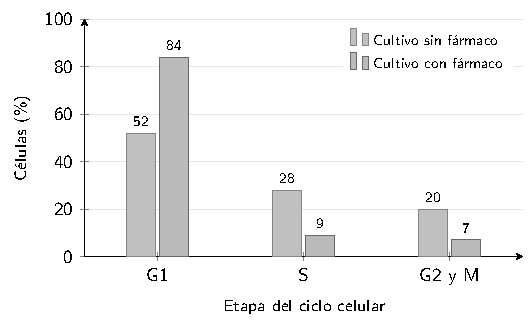
\includegraphics[max width=0.92\linewidth,max height=8.5cm]{bio/div_farmaco}
\end{center}
\altslargas{Acelera la replicación del ADN.}{Bloquea la separación de las cromátidas en la anafase.}{Impide que las células pasen de G1 a la fase S.}{Aumenta el número de células que se dividen.}
\solucion{\textbf{Paso 1. ¿Qué nos piden?} Inferir el efecto del fármaco comparando con el cultivo sin fármaco (control).

\textbf{Paso 2. Compara las barras.} Con el fármaco, las células en G1 suben de 52 \% a 84 \%. Las células en S bajan de 28 \% a 9 \% y las de G2 y M bajan de 20 \% a 7 \%.

\textbf{Paso 3. Interpreta.} Las células se acumulan en G1 y llegan menos a las etapas siguientes: el fármaco frena el paso de G1 a S. Es como si activara el punto de control G1--S.

\textbf{Respuesta:} impide que las células pasen de G1 a la fase S.

\textbf{¿Por qué no las otras?} Si acelerara la replicación no habría menos células en S y más en G1. Si bloqueara la anafase, las células se acumularían en M, pero ese grupo bajó. Hay menos células en S, G2 y M, así que se dividen menos, no más.

\textbf{\color{cienciaD}Para recordar.} Si las células se acumulan en una etapa, el fármaco bloquea el paso a la siguiente.}{C}
\end{elejemplo}
\motivacion{Interfase, cromatina y control del ciclo: ya sabes cómo se prepara una célula para dividirse. Prepárate tú de la misma forma.}

%% =====================================================================
%% bio_mitosis
\section[Mitosis]{Mitosis}
\modcomun\ \ {\color{gris}\itshape Las etapas de la mitosis (profase, metafase, anafase y telofase) y la citocinesis, cómo reconocerlas en un dibujo y su importancia para conservar la información genética, crecer, desarrollarse y reparar tejidos.\par}
\subsection{Qué es la mitosis y para qué sirve}
La \textbf{mitosis} es la división del núcleo que produce \textbf{dos núcleos con la misma información genética} que la célula original. Le sigue la \textbf{citocinesis}, que reparte el citoplasma: el resultado son dos células hijas idénticas entre sí y a la célula madre.

 

Si la célula madre es diploide (2n), las hijas también lo son: \textbf{2n \ensuremath{\rightarrow} 2n}.

 

La mitosis permite:

 
\begin{itemize}
  \item \textbf{Conservar la información genética:} cada célula del cuerpo tiene los mismos cromosomas que el cigoto del que proviene.
  \item \textbf{Crecer y desarrollarse:} de un cigoto se llega a un cuerpo con billones de células.
  \item \textbf{Reparar tejidos:} reemplazar células de la piel, cerrar una herida o soldar un hueso.
  \item \textbf{Reproducirse asexualmente:} levaduras, esquejes de plantas, estolones de la frutilla.
\end{itemize}
  
\begin{clave}[{La clave de la mitosis}] Antes de dividirse, en la fase S, cada cromosoma se copió: tiene dos cromátidas hermanas idénticas. En la mitosis esas cromátidas se separan y \textbf{cada célula hija recibe una copia de cada cromosoma}. Por eso las hijas son idénticas.\end{clave}
 
\begin{clave}[{Recuerda}] La mitosis ocurre en las células del cuerpo (somáticas). Los gametos se forman por meiosis.\end{clave}
\subsection{Profase y metafase}
\textbf{Profase.}

 
\begin{itemize}
  \item La cromatina se \textbf{condensa}: aparecen los cromosomas, cada uno con dos cromátidas hermanas.
  \item Desaparece el nucléolo y la \textbf{envoltura nuclear se desorganiza}.
  \item Los centrosomas (con sus centriolos, en células animales) se van a polos opuestos y entre ellos se arma el \textbf{huso mitótico}, hecho de microtúbulos.
  \item Los microtúbulos se unen a los cromosomas en el centrómero, en unas estructuras de proteína llamadas \textbf{cinetocoros}.
\end{itemize}
  

\textbf{Metafase.}

 
\begin{itemize}
  \item Los cromosomas, con su máxima condensación, se ordenan en el \textbf{plano ecuatorial} de la célula (placa metafásica).
  \item Cada cromátida hermana queda unida a fibras de un polo distinto.
  \item Actúa el \textbf{punto de control de metafase}: la anafase no comienza hasta que todos los cromosomas estén unidos al huso.
\end{itemize}
 
\begin{clave}[{Recuerda}] En la profase y la metafase los cromosomas siguen siendo duplicados: cada uno tiene dos cromátidas hermanas unidas por el centrómero.\end{clave}
\subsection{Anafase, telofase y citocinesis}
\textbf{Anafase.} Se rompen las uniones entre las cromátidas hermanas, que se \textbf{separan} y son arrastradas a polos opuestos por las fibras del huso. Desde ese momento cada cromátida es un cromosoma simple. Es la etapa más corta.

 

\textbf{Telofase.} Los cromosomas llegan a los polos y se \textbf{descondensan}. Se forma una envoltura nuclear alrededor de cada grupo y reaparece el nucléolo: hay dos núcleos.

  

\textbf{Citocinesis.} Se divide el citoplasma:

 
\begin{itemize}
  \item En \textbf{células animales}, un anillo de actina y miosina estrangula la célula desde afuera hacia adentro: el \textbf{surco de segmentación}.
  \item En \textbf{células vegetales}, la pared rígida no deja estrangular: vesículas del aparato de Golgi forman en el centro una \textbf{placa celular} que crece hacia los bordes y da origen a la nueva pared.
\end{itemize}
  
\begin{center}
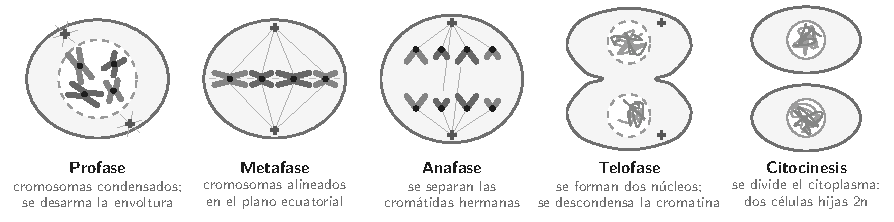
\includegraphics[max width=0.92\linewidth,max height=8.5cm]{bio/div_mitosis}
\end{center}
\subsection{Cómo reconocer cada etapa en un dibujo}
\begin{center}\small
\begin{tabularx}{\linewidth}{@{}>{\raggedright\arraybackslash\hsize=1.29\hsize}X>{\raggedright\arraybackslash\hsize=0.71\hsize}X@{}}
\toprule
\textbf{Si ves\dots{}} & \textbf{La etapa es\dots{}} \\
\midrule
núcleo con envoltura y cromatina sin cromosomas visibles & interfase \\
cromosomas duplicados condensándose; envoltura que se desarma & profase \\
cromosomas duplicados en fila en el centro de la célula & metafase \\
dos grupos de cromosomas simples (en forma de V) que van a los polos & anafase \\
dos núcleos que se reorganizan en los polos; surco o placa celular & telofase y citocinesis \\
\bottomrule
\end{tabularx}
\end{center}
  
\begin{clave}[{Pistas para reconocer}] Mira la forma de los cromosomas: en X tienen dos cromátidas (todavía no se separan); en V o bastón tienen una (ya se separaron). Luego mira dónde están: dispersos en el núcleo, en fila al centro o yendo hacia los polos.\end{clave}
  
\begin{ejemplo}[{Ejemplo resuelto}] En un dibujo hay una célula con dos grupos de cromosomas en forma de V que se alejan hacia polos opuestos. Son cromátidas hermanas que se separan: es una \textbf{anafase}. Cada célula hija recibirá una copia de cada cromosoma.\end{ejemplo}
\subsection{Lo clave del tema}
\begin{center}\small
\begin{tabularx}{\linewidth}{@{}>{\raggedright\arraybackslash\hsize=0.45\hsize}X>{\raggedright\arraybackslash\hsize=1.28\hsize}X>{\raggedright\arraybackslash\hsize=1.28\hsize}X@{}}
\toprule
\textbf{Etapa} & \textbf{Evento principal} & \textbf{Cómo se ven los cromosomas} \\
\midrule
Profase & condensación, se desarma la envoltura, se forma el huso & duplicados (en X), condensándose \\
Metafase & alineación en el plano ecuatorial; punto de control & duplicados (en X), en fila al centro \\
Anafase & separación de las cromátidas hermanas & simples (en V), hacia los polos \\
Telofase & dos núcleos; descondensación & simples, descondensándose en cada núcleo \\
Citocinesis & división del citoplasma (surco o placa celular) & dos células 2n idénticas \\
\bottomrule
\end{tabularx}
\end{center}
 
\begin{clave}[{Recuerda}] · En la anafase de la mitosis se separan las cromátidas hermanas.\par · Las células hijas tienen el mismo número de cromosomas que la madre: 2n \ensuremath{\rightarrow} 2n.\par · La mitosis conserva la información genética: sirve para crecer, desarrollarse, reparar tejidos y reproducirse asexualmente.\end{clave}
 
\begin{clave}[{Método PAES}] 1. Para reconocer una etapa, mira la envoltura nuclear, la posición de los cromosomas y su forma (X o V). 2. En una tabla de duraciones, relaciona cada etapa con su evento. 3. Si un fármaco afecta un componente (huso, actina, cohesión), deduce en qué etapa quedan detenidas las células.\end{clave}
\begin{elejemplo}{PAES Regular 2026, adaptada}
Una profesora muestra a su curso el siguiente esquema, con cuatro células de un mismo tejido en distintas etapas de la mitosis, numeradas al azar:

¿En qué orden ocurren estas etapas?
\begin{center}
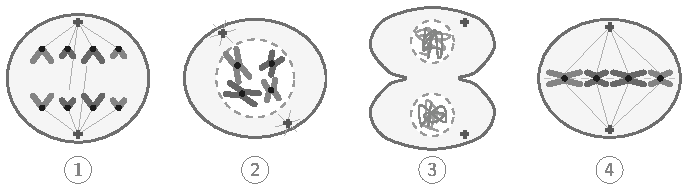
\includegraphics[max width=0.92\linewidth,max height=8.5cm]{bio/div_mitosis_q}
\end{center}
\alts{4, 2, 1 y 3.}{2, 4, 1 y 3.}{2, 1, 4 y 3.}{3, 2, 4 y 1.}
\solucion{\textbf{Paso 1. ¿Qué nos piden?} Ordenar las cuatro células según la secuencia de la mitosis.

\textbf{Paso 2. Identifica cada célula.} Célula 2: cromosomas duplicados condensándose y envoltura que se desarma \ensuremath{\rightarrow} \textbf{profase}. Célula 4: cromosomas duplicados en fila en el centro \ensuremath{\rightarrow} \textbf{metafase}. Célula 1: cromosomas simples en forma de V que van a los polos \ensuremath{\rightarrow} \textbf{anafase}. Célula 3: dos núcleos en formación y la célula estrangulándose \ensuremath{\rightarrow} \textbf{telofase} con citocinesis.

\textbf{Paso 3. Ordena.} Profase, metafase, anafase y telofase: 2, 4, 1 y 3.

\textbf{Respuesta:} 2, 4, 1 y 3.

\textbf{¿Por qué no las otras?} «4, 2, 1 y 3» pone la metafase antes que la profase, pero los cromosomas primero se condensan y después se alinean. «2, 1, 4 y 3» pone la anafase antes que la metafase: las cromátidas solo se separan una vez que todos los cromosomas están alineados. «3, 2, 4 y 1» empieza con la telofase, que es la última etapa.

\textbf{\color{cienciaD}Para recordar.} Profase, metafase, anafase, telofase: condensar, alinear, separar, rehacer los núcleos.}{B}
\end{elejemplo}
\motivacion{Profase, metafase, anafase y telofase: ya las ordenas sin pensarlo. Tu conocimiento también se multiplica.}

%% =====================================================================
%% bio_meiosis
\section[Meiosis y variabilidad genética]{Meiosis y variabilidad genética}
\modcomun\ \ {\color{gris}\itshape Las etapas de la meiosis I y II, el entrecruzamiento y la permutación cromosómica, el paso de células 2n a células n, la comparación con la mitosis y su aporte a la variabilidad genética.\par}
\subsection{Qué es la meiosis y para qué sirve}
La \textbf{meiosis} es la división que forma las células sexuales. Ocurre en las \textbf{células germinales} de las gónadas: en los testículos (espermatozoides) y los ovarios (ovocitos). En las plantas ocurre en las anteras y en los óvulos de la flor.

 

Tiene tres rasgos que la definen:

 
\begin{itemize}
  \item Una sola replicación del ADN, seguida de \textbf{dos divisiones}: meiosis I y meiosis II.
  \item Reduce a la mitad el número de cromosomas: de una célula \textbf{2n} salen células \textbf{n} (haploides), con un cromosoma de cada par.
  \item Las cuatro células que produce son \textbf{genéticamente distintas} entre sí y distintas de la célula madre.
\end{itemize}
  
\begin{clave}[{¿Por qué reducir a la mitad?}] En la fecundación se unen dos gametos. Si cada uno fuera 2n, el cigoto sería 4n y el número de cromosomas se duplicaría en cada generación. Con gametos n (en humanos, 23 cromosomas), el cigoto vuelve a ser 2n = 46.\end{clave}
 
\begin{clave}[{Recuerda}] Meiosis: 2n \ensuremath{\rightarrow} n, cuatro células distintas. Fecundación: n + n \ensuremath{\rightarrow} 2n.\end{clave}
\subsection{Meiosis I: se separan los homólogos}
La célula llega a la meiosis con el ADN ya replicado: cada cromosoma tiene dos cromátidas.

 
\begin{itemize}
  \item \textbf{Profase I.} Es la etapa más larga. Los cromosomas se condensan y cada par de \textbf{homólogos se aparea} a lo largo (sinapsis), unidos por el complejo sinaptonémico. Cada par forma un \textbf{bivalente} o tétrada (cuatro cromátidas). Ocurre el \textbf{entrecruzamiento}.
  \item \textbf{Metafase I.} Los \textbf{pares de homólogos} se ubican en el plano ecuatorial, uno a cada lado.
\end{itemize}
  
\begin{itemize}
  \item \textbf{Anafase I.} Se separan los \textbf{cromosomas homólogos} y van a polos opuestos. Las cromátidas hermanas siguen unidas.
  \item \textbf{Telofase I.} Se forman dos células \textbf{haploides (n)}, cada una con un cromosoma de cada par, todavía con dos cromátidas.
\end{itemize}
 
\begin{clave}[{Recuerda}] La meiosis I es la \textbf{división reduccional}: es la que reduce el número de cromosomas de 2n a n.\end{clave}
  
\begin{center}
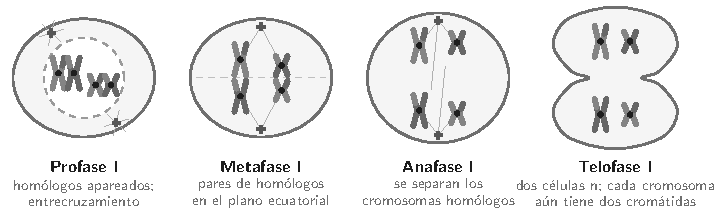
\includegraphics[max width=0.92\linewidth,max height=8.5cm]{bio/div_meiosis1}
\end{center}
\subsection{Meiosis II: se separan las cromátidas}
Entre la meiosis I y la meiosis II \textbf{no hay replicación del ADN}. La meiosis II se parece a una mitosis, pero en células haploides:

 
\begin{itemize}
  \item \textbf{Profase II:} los cromosomas se condensan y se forma un nuevo huso.
  \item \textbf{Metafase II:} los cromosomas, cada uno con dos cromátidas, se alinean en el plano ecuatorial.
  \item \textbf{Anafase II:} se separan las \textbf{cromátidas hermanas} hacia polos opuestos.
  \item \textbf{Telofase II:} se forman los núcleos y se divide el citoplasma.
\end{itemize}
  
\begin{clave}[{Resultado}] De una célula 2n salen \textbf{cuatro células n}, cada una con cromosomas de una cromátida. Gracias al entrecruzamiento, ni siquiera las cromátidas hermanas son ya idénticas: por eso las cuatro células son distintas.\end{clave}
 
\begin{clave}[{Recuerda}] Meiosis I separa homólogos (2n \ensuremath{\rightarrow} n). Meiosis II separa cromátidas hermanas (n \ensuremath{\rightarrow} n).\end{clave}
  
\begin{center}
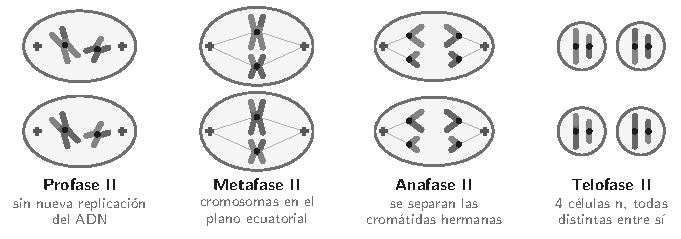
\includegraphics[max width=0.92\linewidth,max height=8.5cm]{bio/div_meiosis2}
\end{center}
\subsection{Entrecruzamiento (crossing-over)}
Durante la profase I, cuando los homólogos están apareados, una cromátida de cada homólogo se corta en el mismo punto y ambas \textbf{intercambian segmentos}. El punto donde quedan unidas se ve como una X y se llama \textbf{quiasma}.

 

Resultado: aparecen \textbf{cromátidas recombinantes}, con una combinación de alelos que no existía en los cromosomas de la madre ni del padre.

 

En el ejemplo, un homólogo tenía los alelos A y B, y el otro, a y b. Tras el entrecruzamiento hay cuatro cromátidas distintas: AB, aB, Ab y ab.

  
\begin{clave}[{Los quiasmas también sirven para repartir bien}] Mantienen unidos a los homólogos hasta la anafase I, para que cada uno vaya a un polo distinto. Si se forman pocos quiasmas, aumenta el riesgo de que un par no se separe (\textbf{no disyunción}) y se formen gametos con un cromosoma de más o de menos.\end{clave}
  
\begin{center}
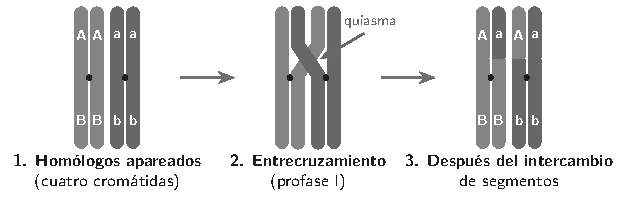
\includegraphics[max width=0.92\linewidth,max height=8.5cm]{bio/div_crossing}
\end{center}
\subsection{Permutación cromosómica y fecundación}
En la metafase I, cada par de homólogos se orienta \textbf{al azar}: el cromosoma materno puede quedar mirando a cualquiera de los dos polos, sin importar cómo se ordenan los otros pares. A esto se le llama \textbf{permutación cromosómica} o segregación independiente.

 

Con n pares de cromosomas hay \textbf{2\textsuperscript{n}} combinaciones posibles de cromosomas en los gametos (sin contar el entrecruzamiento).

 
\begin{itemize}
  \item Con 2 pares: 2\textsuperscript{2} = 4 combinaciones.
  \item En humanos, con 23 pares: 2\textsuperscript{23}, más de 8 millones.
\end{itemize}
  
\begin{center}
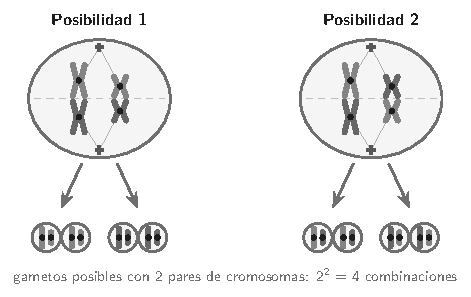
\includegraphics[max width=0.92\linewidth,max height=8.5cm]{bio/div_permutacion}
\end{center}
 
\begin{clave}[{Las fuentes de variabilidad genética}] · \textbf{Mutaciones:} crean alelos nuevos.\par · \textbf{Entrecruzamiento} (profase I): mezcla alelos dentro de un cromosoma.\par · \textbf{Permutación cromosómica} (metafase I): mezcla cromosomas maternos y paternos.\par · \textbf{Fecundación al azar:} cualquier óvulo con cualquier espermatozoide.\end{clave}
\subsection{Lo clave del tema}
\begin{center}\small
\begin{tabularx}{\linewidth}{@{}>{\raggedright\arraybackslash\hsize=0.94\hsize}X>{\raggedright\arraybackslash\hsize=1.12\hsize}X>{\raggedright\arraybackslash\hsize=0.94\hsize}X@{}}
\toprule
 & \textbf{Mitosis} & \textbf{Meiosis} \\
\midrule
Células que la hacen & somáticas & germinales (gónadas) \\
Divisiones & una & dos, tras una sola replicación \\
Células resultantes & 2, diploides (2n), idénticas & 4, haploides (n), distintas \\
Apareamiento y entrecruzamiento & no ocurren & sí, en la profase I \\
Qué se separa en la anafase & cromátidas hermanas & homólogos (I) y cromátidas (II) \\
Función & crecer, reparar, reproducción asexual & formar gametos, variabilidad \\
\bottomrule
\end{tabularx}
\end{center}
 
\begin{clave}[{Recuerda}] · En la anafase I se separan los cromosomas homólogos; en la anafase II, las cromátidas hermanas.\par · Las células que salen de la meiosis I ya son haploides, aunque sus cromosomas tengan dos cromátidas.\par · La variabilidad viene del entrecruzamiento (profase I), la permutación (metafase I) y la fecundación al azar.\end{clave}
 
\begin{clave}[{Método PAES}] 1. En un dibujo, mira qué se mueve hacia los polos: cromosomas en forma de X (homólogos, anafase I) o en forma de V (cromátidas, anafase II o mitosis). 2. Mira cada polo: si tiene pares de homólogos es 2n; si tiene uno de cada tipo es n. 3. Para la variabilidad, usa 2\textsuperscript{n} y suma el entrecruzamiento.\end{clave}
\begin{elejemplo}{PAES Invierno 2026, adaptada}
El siguiente dibujo muestra una célula en división, obtenida del testículo de un animal. Los colores indican el origen de cada cromosoma (materno o paterno):

¿En qué etapa está la célula y cuál es el número diploide de la especie?
\begin{center}
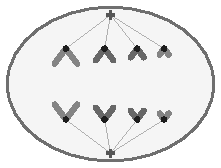
\includegraphics[max width=0.92\linewidth,max height=8.5cm]{bio/div_anafase2_q}
\end{center}
\alts{Anafase de la mitosis; 2n = 4.}{Anafase II de la meiosis; 2n = 8.}{Anafase I de la meiosis; 2n = 8.}{Anafase II de la meiosis; 2n = 4.}
\solucion{\textbf{Paso 1. ¿Qué nos piden?} La etapa de la célula y el número 2n de la especie.

\textbf{Paso 2. ¿Qué se separa?} Los cromosomas tienen forma de V: son cromátidas sueltas. Se están separando cromátidas hermanas: puede ser una mitosis o una anafase II.

\textbf{Paso 3. Mira cada polo.} Cada polo recibe cuatro cromosomas, todos de tamaño distinto: hay \textbf{uno de cada tipo}, sin pares de homólogos. La célula es haploide: es una \textbf{anafase II} y n = 4.

\textbf{Paso 4. Número diploide.} Si n = 4, la especie tiene 2n = 8.

\textbf{Respuesta:} anafase II de la meiosis; 2n = 8.

\textbf{¿Por qué no las otras?} En una mitosis cada polo tendría pares de cromosomas del mismo tamaño. En la anafase I se mueven cromosomas con dos cromátidas (forma de X). 2n = 4 confunde el número de cromosomas de cada polo (4, que es n) con el número diploide.

\textbf{\color{cienciaD}Para recordar.} Cromátidas que se separan y polos sin pares de homólogos: anafase II.}{B}
\end{elejemplo}
\motivacion{La meiosis crea variabilidad, y la variabilidad hace única a cada persona. Tú también tienes tu forma única de aprender.}

%% =====================================================================
%% bio_ingenieria
\section[Manipulación genética]{Manipulación genética}
\modcomun\ \ {\color{gris}\itshape Qué es la manipulación genética, el ADN recombinante y los organismos transgénicos; aplicaciones en alimentos, detergentes, vestuario y fármacos como la insulina humana producida por bacterias; y los beneficios, riesgos y debates que generan.\par}
\subsection{Qué es la manipulación genética}
La \textbf{manipulación genética} (o ingeniería genética) es el conjunto de técnicas que permiten \textbf{modificar el ADN} de un organismo: cortar un gen, copiarlo, cambiarlo o llevarlo de una especie a otra.

 

Cuando se une ADN de dos orígenes distintos (por ejemplo, un gen humano dentro de ADN bacteriano) se obtiene \textbf{ADN recombinante}.

 

Un organismo que lleva en su ADN un gen de \textbf{otra especie} es un \textbf{organismo transgénico} (un tipo de organismo genéticamente modificado, OGM).

  
\begin{clave}[{¿Por qué funciona?}] El \textbf{código genético es universal}: casi todos los seres vivos leen el ADN con las mismas reglas. Por eso una bacteria que recibe el gen humano de la insulina fabrica insulina humana.\end{clave}
 
\begin{clave}[{Recuerda}] Transgénico: tiene un gen de otra especie. Un clon (como la oveja Dolly) es una copia genética de otro individuo, sin genes de otra especie.\end{clave}
\subsection{Aplicaciones}
\begin{center}\small
\begin{tabularx}{\linewidth}{@{}>{\raggedright\arraybackslash\hsize=0.45\hsize}X>{\raggedright\arraybackslash\hsize=1.28\hsize}X>{\raggedright\arraybackslash\hsize=1.28\hsize}X@{}}
\toprule
\textbf{Área} & \textbf{Ejemplo} & \textbf{Cómo se logra} \\
\midrule
Alimentos & maíz y soya resistentes a insectos; arroz dorado con provitamina A & se agrega el gen de la toxina Bt de la bacteria \emph{Bacillus thuringiensis}; genes para fabricar betacaroteno en el grano \\
Detergentes & enzimas que eliminan manchas en agua fría & microorganismos modificados producen en gran cantidad proteasas (proteínas), lipasas (grasas) y amilasas (almidón) \\
Vestuario & algodón Bt & la planta fabrica la toxina Bt y resiste a las larvas que dañan el capullo de fibra; se aplican menos insecticidas \\
Fármacos & insulina humana, hormona del crecimiento, vacuna contra la hepatitis B & bacterias o levaduras con el gen humano producen la proteína \\
\bottomrule
\end{tabularx}
\end{center}
 
\begin{clave}[{Recuerda}] En todas estas aplicaciones el organismo modificado fabrica una proteína nueva porque recibió el gen que la codifica: la toxina Bt, una enzima o una hormona humana.\end{clave}
\subsection{La insulina humana producida por bacterias}
Las personas con diabetes tipo 1 no producen insulina y deben inyectársela. Hasta los años ochenta, la insulina se extraía del páncreas de cerdos y vacas: hacían falta miles de páncreas, y la insulina animal es levemente distinta de la humana.

 

En 1982 se aprobó la primera insulina humana fabricada por bacterias con el gen humano. Fue el primer medicamento obtenido por ingeniería genética.

  
\begin{clave}[{Ventajas}] · Es \textbf{idéntica} a la insulina humana.\par · Se produce en \textbf{grandes cantidades} en fermentadores, sin depender de animales.\par · Su calidad es constante de un lote a otro.\end{clave}
 
\begin{clave}[{Recuerda}] La bacteria no se convierte en célula humana: solo lleva un gen humano y fabrica la proteína que ese gen codifica.\end{clave}
\subsection{Beneficios, riesgos y debates}
\textbf{Beneficios.} Más producción con menos insecticidas, alimentos más nutritivos, medicamentos seguros y abundantes, procesos industriales que ahorran energía y agua.

 

\textbf{Riesgos que se investigan.}

 
\begin{itemize}
  \item Que un gen transgénico pase por polinización a plantas silvestres emparentadas.
  \item Que las plagas se vuelvan resistentes a la toxina Bt.
  \item Que una proteína nueva provoque alergias.
\end{itemize}
  
\begin{clave}[{Ciencia y sociedad}] Algunas preguntas se responden con experimentos (¿pasa el gen a otras plantas?, ¿causa alergia?). Otras dependen de valores y decisiones de la sociedad (¿se deben patentar los seres vivos?, ¿cómo se etiquetan los alimentos?). Ambas son parte del debate, pero se responden de forma distinta.\end{clave}
\subsection{Lo clave del tema}
\begin{center}\small
\begin{tabularx}{\linewidth}{@{}>{\raggedright\arraybackslash\hsize=0.77\hsize}X>{\raggedright\arraybackslash\hsize=1.23\hsize}X@{}}
\toprule
\textbf{Concepto} & \textbf{Qué es} \\
\midrule
Manipulación genética & técnicas para modificar el ADN: cortar un gen, copiarlo o llevarlo de una especie a otra \\
ADN recombinante & ADN formado al unir ADN de dos orígenes distintos \\
Organismo transgénico & lleva en su ADN un gen de otra especie y lo expresa \\
Clon & copia genética de otro individuo, sin genes de otra especie \\
Código genético universal & casi todos los seres vivos leen el ADN con las mismas reglas: por eso una bacteria fabrica una proteína humana \\
\bottomrule
\end{tabularx}
\end{center}
 
\begin{clave}[{Recuerda}] · Un organismo transgénico lleva un gen de otra especie y lo expresa gracias a que el código genético es universal.\par · Un clon o una planta obtenida al cruzar dos variedades de la misma especie no son transgénicos.\par · La insulina producida por bacterias es idéntica a la humana y se fabrica en grandes cantidades.\end{clave}
 
\begin{clave}[{Método PAES}] 1. Para reconocer un transgénico, pregúntate si recibió un gen de otra especie. 2. En las aplicaciones, nombra qué gen se agregó y qué ventaja da. 3. En los detergentes, relaciona cada enzima con lo que digiere: proteasas, proteínas; lipasas, grasas; amilasas, almidón. 4. En un debate, distingue las preguntas que se responden con experimentos de las que dependen de valores.\end{clave}
\begin{elejemplo}{PAES Invierno 2026, adaptada}
El arroz no fabrica betacaroteno (provitamina A) en su grano. Para obtener «arroz dorado», un equipo identificó dos genes, uno de narciso y otro de una bacteria, que codifican las enzimas necesarias para fabricar betacaroteno.

¿Cuál de los siguientes pasos es indispensable para obtener este arroz transgénico?
\altslargas{Regar las plantas de arroz con una solución de betacaroteno.}{Insertar los dos genes en el ADN de células de arroz, de modo que se expresen en el grano.}{Cruzar plantas de arroz con plantas de narciso.}{Inyectar en las semillas las enzimas ya fabricadas por la bacteria.}
\solucion{\textbf{Paso 1. ¿Qué nos piden?} El paso que no puede faltar para obtener un arroz transgénico.

\textbf{Paso 2. Recuerda la definición.} Un organismo transgénico lleva en su \textbf{ADN} genes de otra especie, y los expresa. Para que el arroz fabrique betacaroteno y lo herede a la siguiente generación, los genes deben quedar en el ADN de sus células.

\textbf{Respuesta:} insertar los dos genes en el ADN de células de arroz, de modo que se expresen en el grano.

\textbf{¿Por qué no las otras?} Regar con betacaroteno no cambia el ADN: la planta no aprendería a fabricarlo. Arroz y narciso son especies distintas que no pueden cruzarse. Inyectar las enzimas solo dura hasta que se degraden y no pasa a la descendencia, porque no hay un gen nuevo.

\textbf{\color{cienciaD}Para recordar.} Transgénico: el gen de otra especie se integra en el ADN y se expresa.}{B}
\end{elejemplo}
\motivacion{Transgénicos, clonación y edición genética: ya puedes opinar con fundamentos. Eso es ciencia con criterio.}

%% =====================================================================
%% bio_evidencias
\section[Evidencias de la evolución]{Evidencias de la evolución}
\modcomun\ \ {\color{gris}\itshape Cómo sabemos que las especies evolucionan: anatomía comparada (estructuras homólogas, análogas y vestigiales), embriología, comparación de secuencias de ADN y proteínas, registro fósil y lectura de árboles filogenéticos.\par}
\subsection{La evolución y sus evidencias}
La \textbf{evolución biológica} es el cambio en las características heredables de las \textbf{poblaciones} a lo largo de muchas generaciones. Una de sus ideas centrales es la \textbf{descendencia con modificación}: las especies actuales descienden de especies anteriores, y dos especies cualesquiera comparten, en algún momento del pasado, un \textbf{ancestro común}.

 

Esta idea es una \textbf{teoría científica}: una explicación amplia, puesta a prueba muchas veces y respaldada por evidencias de áreas muy distintas que apuntan a la misma conclusión.

 
\begin{itemize}
  \item \textbf{Anatomía comparada:} se comparan estructuras del cuerpo de especies actuales.
  \item \textbf{Embriología comparada:} se compara el desarrollo de los embriones.
  \item \textbf{Biología molecular:} se comparan secuencias de ADN y de proteínas.
  \item \textbf{Registro fósil:} se estudian restos de organismos del pasado conservados en las rocas.
\end{itemize}
  
\begin{clave}[{La pregunta que se repite}] En todas estas evidencias la PAES pregunta lo mismo: \textbf{¿qué tan emparentadas están estas especies?} Mientras más rasgos compartan por haberlos heredado de un ancestro (huesos, etapas del embrión, secuencias de ADN), más reciente es su ancestro común.\end{clave}
 
\begin{clave}[{Recuerda}] Evolucionan las poblaciones, a lo largo de generaciones. Un individuo no evoluciona durante su vida: crece, aprende o se entrena, pero esos cambios no modifican el ADN de sus gametos.\end{clave}
\subsection{Anatomía comparada: estructuras homólogas}
Las \textbf{estructuras homólogas} tienen el \textbf{mismo origen embrionario} y el \textbf{mismo plan básico}, aunque hoy cumplan funciones distintas.

 

El ejemplo clásico son las extremidades anteriores de los mamíferos. El brazo humano, la pata del gato, la aleta de la ballena y el ala del murciélago sirven para tomar objetos, caminar, nadar y volar, pero todas tienen la misma secuencia de huesos: un \textbf{húmero}, luego \textbf{radio y cúbito}, luego los \textbf{carpos} y al final \textbf{metacarpos y falanges}.

 

Lo que cambia es la forma y el largo de cada hueso: dedos muy largos que sostienen la membrana del ala en el murciélago, huesos cortos y anchos dentro de la aleta en la ballena.

 

\textbf{Qué indican:} que estas especies heredaron ese plan de un \textbf{ancestro común}. A partir de él, cada linaje se fue adaptando a ambientes distintos: es la \textbf{evolución divergente}.

  
\begin{center}
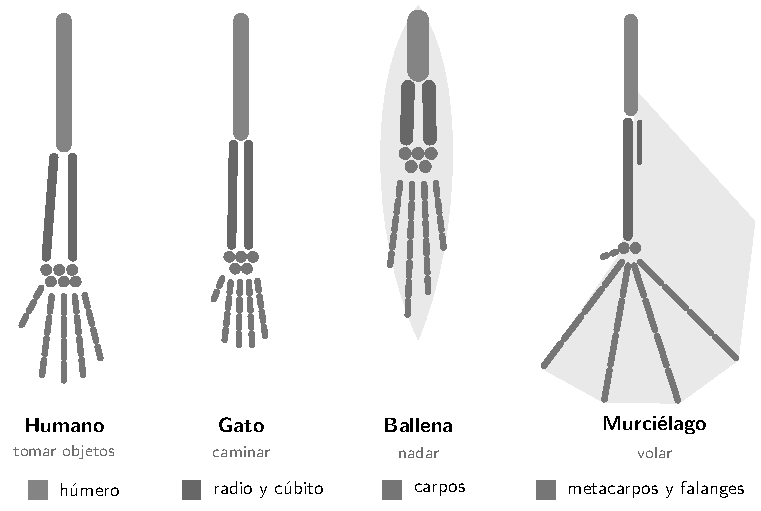
\includegraphics[max width=0.92\linewidth,max height=8.5cm]{bio/evo_extremidades}
\end{center}
\subsection{Estructuras análogas, vestigiales y embriología}
\textbf{Estructuras análogas.} Cumplen la \textbf{misma función}, pero tienen \textbf{distinto origen} y distinta estructura interna. El ala de una mariposa es una lámina sin huesos; el ala de un ave está sostenida por huesos. Otros ejemplos: el ojo del pulpo y el ojo humano, o la forma hidrodinámica del tiburón y la del delfín. Indican \textbf{evolución convergente}: ambientes o modos de vida parecidos favorecieron soluciones parecidas en linajes poco emparentados.

 

\textbf{Estructuras vestigiales.} Son estructuras \textbf{reducidas}, que no cumplen función o cumplen una función menor que en los ancestros. Ejemplos: los pequeños huesos de la cadera (pelvis) dentro del cuerpo de las ballenas, el cóccix humano y las alas diminutas del kiwi. Indican que la especie desciende de ancestros en los que esa estructura estaba desarrollada.

  

\textbf{Embriología comparada.} En las primeras etapas del desarrollo, los embriones de peces, aves y mamíferos se parecen mucho: todos tienen \textbf{arcos y hendiduras faríngeas} y una \textbf{cola}. Después, cada uno sigue su camino: en los peces los arcos faríngeos originan las branquias y en los mamíferos originan partes de la mandíbula, del oído medio y del cuello. Este desarrollo compartido indica un \textbf{ancestro común} de los vertebrados.

 
\begin{clave}[{Recuerda}] · Homólogas: mismo origen, función distinta \ensuremath{\rightarrow} ancestro común (divergencia).\par · Análogas: misma función, origen distinto \ensuremath{\rightarrow} convergencia.\par · Las alas del ave y del murciélago son homólogas como extremidades anteriores (mismos huesos), y análogas como alas: el vuelo surgió por separado en cada grupo.\par · Las hendiduras faríngeas del embrión humano originan estructuras de la cabeza y el cuello; el ser humano respira con pulmones.\end{clave}
\subsection{Biología molecular}
Todos los seres vivos usan el ADN como material genético y prácticamente el mismo \textbf{código genético}. Esa universalidad ya es una evidencia de un origen común.

 

Además, se pueden comparar las \textbf{secuencias de nucleótidos} de un mismo gen, o las \textbf{secuencias de aminoácidos} de una misma proteína, en distintas especies. Las diferencias se acumulan con el tiempo por mutaciones. Por eso:

 
\begin{clave}[{Regla de lectura}] Mientras \textbf{menos diferencias} (o más porcentaje de similitud) haya entre dos especies, \textbf{más reciente} es su ancestro común y más estrecho su parentesco.\end{clave}
 

\textbf{Ejemplo real:} el citocromo c, una proteína de la respiración celular, es idéntico en el ser humano y el chimpancé, y difiere en más de 40 aminoácidos entre el ser humano y la levadura.

 

Esta evidencia es muy útil cuando la anatomía engaña: dos especies pueden verse parecidas por convergencia, pero sus secuencias revelan su parentesco real.

  
\begin{center}
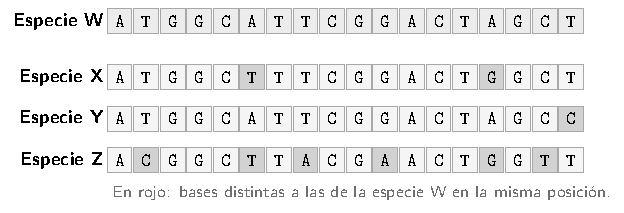
\includegraphics[max width=0.92\linewidth,max height=8.5cm]{bio/evo_secuencias}
\end{center}
 
\begin{ejemplo}[{Ejemplo resuelto}] En la figura, la especie Y difiere de W en 1 base, X en 2 y Z en 6. De mayor a menor parentesco con W: \textbf{Y, X, Z}.\end{ejemplo}
\subsection{Registro fósil}
Un \textbf{fósil} es un resto (huesos, conchas, dientes) o una huella de un organismo del pasado conservado en las rocas. La mayoría se forma en \textbf{rocas sedimentarias}, que se depositan en capas o \textbf{estratos}.

 

\textbf{Datación relativa.} Si los estratos no han sido alterados, los de abajo se depositaron primero: son \textbf{más antiguos} (principio de superposición). Así se ordenan los fósiles del más antiguo al más reciente, sin saber su edad en años.

 

\textbf{Datación absoluta.} Mide la edad en años usando isótopos radiactivos de las rocas o de los restos, como el carbono-14 para restos de hasta unos 50 000 años.

 

\textbf{Fósiles de transición.} Tienen rasgos de dos grupos. \emph{Archaeopteryx} (unos 150 millones de años) tenía plumas y alas como un ave, y dientes, garras en las alas y una cola larga con huesos como un reptil. \emph{Tiktaalik} (unos 375 millones de años) era un pez con cuello móvil y aletas con huesos similares a los de un brazo.

  
\begin{center}
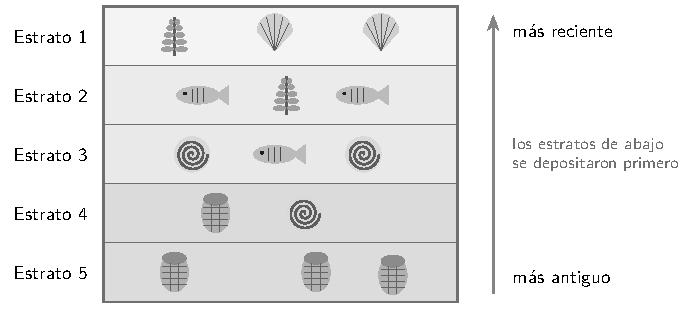
\includegraphics[max width=0.92\linewidth,max height=8.5cm]{bio/evo_estratos}
\end{center}
 
\begin{clave}[{Qué responde y qué no}] Con una columna de estratos se puede responder \textbf{qué especie es más antigua} y \textbf{cuáles vivieron en la misma época} (aparecen en el mismo estrato). No basta para saber la causa de una extinción ni quién desciende de quién.\end{clave}
\subsection{Árboles filogenéticos}
Un \textbf{árbol filogenético} resume las relaciones de parentesco que se deducen de todas las evidencias. Se lee así:

 
\begin{itemize}
  \item Las \textbf{puntas} de las ramas son las especies (actuales o extintas).
  \item Cada \textbf{nodo} (punto donde se separan dos ramas) representa un \textbf{ancestro común}.
  \item Dos especies están más emparentadas mientras \textbf{más reciente} sea el nodo que comparten (más cerca de las puntas).
\end{itemize}
 

En el árbol de la figura, el lagarto y el ave comparten un ancestro más reciente que el que comparten el lagarto y el ratón. Por eso el lagarto está más emparentado con el ave que con el ratón, aunque a simple vista se parezca más al ratón (cuatro patas, sin plumas).

  
\begin{center}
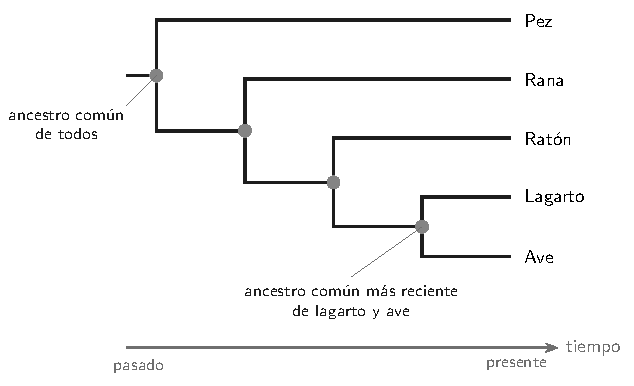
\includegraphics[max width=0.92\linewidth,max height=8.5cm]{bio/evo_arbol}
\end{center}
 
\begin{clave}[{Recuerda}] · Lo que importa son los nodos, no el orden vertical de los nombres: girar las ramas en un nodo no cambia el árbol.\par · Las especies actuales no descienden unas de otras: comparten ancestros. El ser humano y el chimpancé comparten un ancestro común.\end{clave}
\subsection{Lo clave del tema}
\begin{center}\small
\begin{tabularx}{\linewidth}{@{}>{\raggedright\arraybackslash\hsize=0.66\hsize}X>{\raggedright\arraybackslash\hsize=1.06\hsize}X>{\raggedright\arraybackslash\hsize=1.14\hsize}X>{\raggedright\arraybackslash\hsize=1.14\hsize}X@{}}
\toprule
\textbf{Evidencia} & \textbf{Qué se compara} & \textbf{Qué indica} & \textbf{Ejemplo} \\
\midrule
Estructuras homólogas & mismo origen y plan, distinta función & ancestro común (divergencia) & brazo, aleta de ballena, ala de murciélago \\
Estructuras análogas & misma función, distinto origen & convergencia, no parentesco cercano & ala de mariposa y ala de ave \\
Estructuras vestigiales & estructuras reducidas & ancestros con la estructura desarrollada & pelvis de ballena, cóccix \\
Embriología & etapas tempranas del desarrollo & ancestro común & arcos faríngeos y cola en vertebrados \\
Biología molecular & secuencias de ADN o de aminoácidos & menos diferencias = parentesco más cercano & citocromo c \\
Registro fósil & fósiles en estratos & orden de aparición, formas de transición & \emph{Archaeopteryx}, \emph{Tiktaalik} \\
\bottomrule
\end{tabularx}
\end{center}
 
\begin{clave}[{Recuerda}] · Solo las estructuras homólogas indican parentesco; las análogas indican ambientes parecidos.\par · En estratos no alterados, más abajo es más antiguo.\par · Una tabla de diferencias o de similitud indica parentesco, no qué especie apareció primero.\par · En un árbol, el parentesco lo da el nodo compartido más reciente.\end{clave}
 
\begin{clave}[{Método PAES}] 1. Identifica la evidencia (anatomía, embrión, secuencia, fósil). 2. Pregúntate qué permite concluir esa evidencia y qué no (parentesco, orden de antigüedad, causa). 3. En tablas, busca la menor diferencia o la mayor similitud. 4. En árboles, busca el nodo más reciente que une a las especies. 5. Descarta las alternativas que van más allá de los datos.\end{clave}
\begin{elejemplo}{PAES Regular 2026, adaptada}
Un equipo de investigación secuenció el mismo fragmento de un gen en cuatro especies de anfibios, W, X, Y y Z. La figura muestra las secuencias alineadas; en rojo están las bases que difieren de las de la especie W en la misma posición.

A partir de estos datos, ¿cuál de las siguientes opciones ordena las especies X, Y y Z de \textbf{mayor a menor} parentesco con la especie W?
\begin{center}
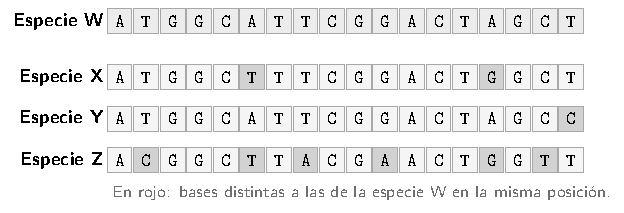
\includegraphics[max width=0.92\linewidth,max height=8.5cm]{bio/evo_secuencias}
\end{center}
\alts{X, Y, Z}{Z, X, Y}{Y, X, Z}{Y, Z, X}
\solucion{\textbf{Paso 1. ¿Qué nos piden?} Ordenar las especies según su parentesco con W, usando la comparación de secuencias de ADN.

\textbf{Paso 2. Cuenta las diferencias.} Recorre cada secuencia y cuenta las bases marcadas: X tiene 2 (posiciones 6 y 15), Y tiene 1 (posición 18) y Z tiene 6.

\textbf{Paso 3. Aplica la regla.} Las diferencias se acumulan con el tiempo desde que dos linajes se separaron. Menos diferencias significa un ancestro común más reciente, es decir, un parentesco más cercano.

\textbf{Respuesta:} Y (1 diferencia), X (2) y Z (6).

\textbf{¿Por qué no las otras?} «X, Y, Z» pone primero a X, que tiene más diferencias que Y. «Z, X, Y» invierte la regla: ordena de menor a mayor parentesco. «Y, Z, X» pone a Z antes que X, aunque Z tiene 6 diferencias y X solo 2.

\textbf{\color{cienciaD}Para recordar.} Menos diferencias en la secuencia = ancestro común más reciente = parentesco más cercano.}{C}
\end{elejemplo}
\motivacion{Fósiles, órganos homólogos y ADN: las evidencias se van sumando. Tus horas de estudio también.}

%% =====================================================================
%% bio_seleccion
\section[Darwin, Wallace y la selección natural]{Darwin, Wallace y la selección natural}
\modcomun\ \ {\color{gris}\itshape Los aportes de Darwin y Wallace, los fundamentos de la selección natural y sus ejemplos (polilla moteada, resistencia a antibióticos y pesticidas, pinzones), y la lectura de gráficos de frecuencia a lo largo de generaciones.\par}
\subsection{Darwin y Wallace}
\textbf{Charles Darwin} viajó alrededor del mundo en el barco \emph{Beagle} (1831-1836), con largas estadías en Sudamérica, incluido Chile, y una visita a las islas Galápagos. Allí notó que especies muy parecidas, como los pinzones y las tortugas, variaban de una isla a otra.

 

Al volver, reunió más evidencias: la \textbf{selección artificial} que hacen los criadores de palomas y ganado, y las ideas de Malthus sobre poblaciones que crecen más rápido que sus recursos.

 

\textbf{Alfred Russel Wallace}, estudiando la fauna del Amazonas y del archipiélago malayo, llegó por su cuenta a la misma explicación. En 1858 le envió a Darwin un ensayo con la idea, y ese mismo año se presentaron juntos los trabajos de ambos en la Sociedad Linneana de Londres.

 

En 1859 Darwin publicó \emph{El origen de las especies}, con abundantes evidencias de la \textbf{evolución por selección natural}.

  
\begin{clave}[{Qué aportó cada uno}] · \textbf{Darwin:} la teoría de la descendencia con modificación y de la selección natural, sostenida con una enorme cantidad de evidencias.\par · \textbf{Wallace:} llegó de forma independiente a la selección natural y estudió la distribución geográfica de las especies (biogeografía).\end{clave}
 
\begin{clave}[{Recuerda}] Darwin y Wallace no conocían los genes. Durante el siglo XX, la genética explicó el origen de la variación (mutaciones y recombinación) y se unió a la selección natural en la \textbf{teoría sintética} de la evolución.\end{clave}
\subsection{Fundamentos de la selección natural}
La selección natural se apoya en cuatro hechos observables:

 
\begin{enumerate}
  \item \textbf{Variación heredable.} Los individuos de una población difieren en sus características, y parte de esas diferencias se heredan.
  \item \textbf{Sobreproducción.} Nacen más individuos de los que el ambiente puede sostener.
  \item \textbf{Lucha por la existencia.} Los recursos son limitados: los individuos compiten por alimento, espacio o pareja, y enfrentan depredadores y enfermedades.
  \item \textbf{Supervivencia y reproducción diferencial.} Los individuos con características más favorables en ese ambiente sobreviven y dejan \textbf{más descendencia}.
\end{enumerate}
 

\textbf{Resultado:} a lo largo de generaciones aumenta en la población la frecuencia de las características favorables. Así se forman las \textbf{adaptaciones}.

  
\begin{clave}[{Adaptación}] Característica heredable que aumenta la supervivencia o la reproducción de un individuo en un ambiente determinado. Lo que cuenta es el \textbf{éxito reproductivo}: un rasgo que atrae más parejas también es adaptativo.\end{clave}
 
\begin{clave}[{Recuerda}] · La variación existe \textbf{antes} del cambio ambiental; surge al azar por mutaciones y recombinación.\par · El ambiente \textbf{selecciona} entre variantes que ya existen.\par · La selección actúa sobre individuos, y lo que cambia es la frecuencia de las características en la \textbf{población}.\end{clave}
\subsection{Ejemplos: polilla moteada y pinzones}
\textbf{Polilla moteada} (\emph{Biston betularia}). En Inglaterra hay polillas claras y oscuras; el color es heredable. Antes de la Revolución Industrial, los troncos estaban cubiertos de líquenes claros y casi todas las polillas eran claras. El hollín de las fábricas oscureció los troncos: las polillas oscuras quedaron mejor camufladas frente a las aves que las cazan, sobrevivieron y se reprodujeron más, y llegaron a ser la gran mayoría. Cuando las leyes redujeron la contaminación, los troncos se aclararon y la tendencia se invirtió.

 

\textbf{Pinzones de Galápagos.} Las distintas especies descienden de un ancestro que llegó desde el continente; sus picos se diversificaron según el alimento de cada ambiente. Peter y Rosemary Grant lo midieron en la isla Daphne Mayor: tras la sequía de 1977 quedaron sobre todo semillas grandes y duras, sobrevivieron más los pinzones de pico más grande y profundo, y la generación siguiente tuvo, en promedio, picos más profundos.

  
\begin{center}
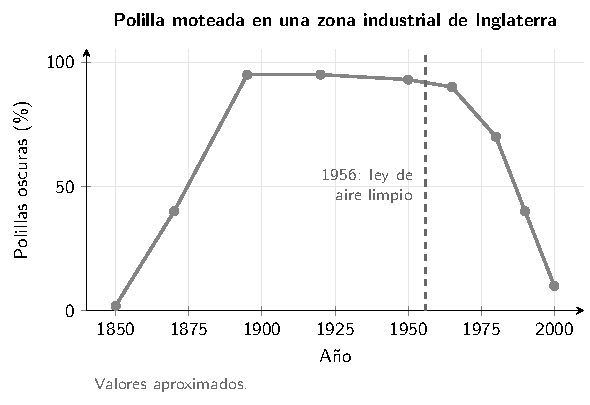
\includegraphics[max width=0.92\linewidth,max height=8.5cm]{bio/evo_polilla}
\end{center}
 
\begin{clave}[{Cómo leer un gráfico de frecuencias}] 1. Mira qué característica se mide y en qué unidad (\% de la población). 2. Ubica cuándo cambia el ambiente. 3. Describe la tendencia después del cambio: si una variante aumenta generación tras generación, el ambiente la está favoreciendo.\end{clave}
\subsection{Ejemplos: resistencia a antibióticos y pesticidas}
En una población de bacterias hay variación: por \textbf{mutaciones al azar}, o por genes recibidos de otras bacterias, algunas pocas son resistentes a un antibiótico antes de que se use.

 
\begin{enumerate}
  \item Al aplicar el antibiótico, mueren las bacterias sensibles. El antibiótico actúa como \textbf{presión de selección}.
  \item Las resistentes sobreviven y se reproducen, con poca competencia.
  \item Tras varias generaciones, casi toda la población es resistente.
\end{enumerate}
 

Lo mismo ocurre con los \textbf{insectos y los pesticidas}, y con las malezas y los herbicidas: el producto elimina a los sensibles y deja a los que ya eran resistentes.

 

Por eso los antibióticos se usan solo con receta, nunca contra virus (como el resfrío), y el tratamiento se cumple completo, como lo indique el médico.

  
\begin{center}
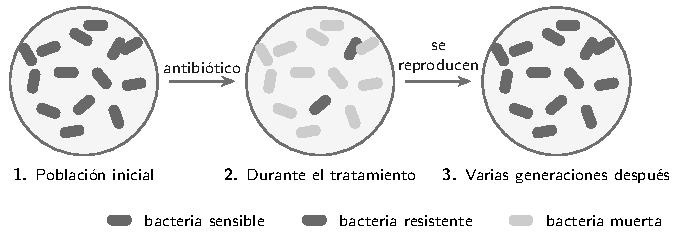
\includegraphics[max width=0.92\linewidth,max height=8.5cm]{bio/evo_bacterias}
\end{center}
 
\begin{clave}[{Recuerda}] El antibiótico no crea la resistencia: selecciona a las bacterias que ya la tenían. La población cambia porque cambia la proporción de bacterias resistentes.\end{clave}
\subsection{Lo clave del tema}
\begin{center}\small
\begin{tabularx}{\linewidth}{@{}>{\raggedright\arraybackslash\hsize=0.79\hsize}X>{\raggedright\arraybackslash\hsize=1.13\hsize}X>{\raggedright\arraybackslash\hsize=1.08\hsize}X@{}}
\toprule
\textbf{Concepto} & \textbf{Idea central} & \textbf{Ejemplo} \\
\midrule
Darwin y Wallace (1858-1859) & evolución por selección natural & pinzones, selección artificial \\
Variación heredable & existe antes del cambio ambiental & polillas claras y oscuras \\
Presión de selección & factor del ambiente que favorece a unas variantes & antibiótico, depredador, sequía \\
Reproducción diferencial & los mejor adaptados dejan más descendencia & pinzones de pico profundo en la sequía \\
Adaptación & rasgo heredable que aumenta la supervivencia o la reproducción & camuflaje, resistencia \\
\bottomrule
\end{tabularx}
\end{center}
 
\begin{clave}[{Recuerda}] · Los caracteres adquiridos durante la vida no se heredan.\par · La variación surge al azar; el ambiente selecciona.\par · Evoluciona la población, no el individuo.\par · Ser adaptativo significa dejar más descendencia en ese ambiente.\end{clave}
 
\begin{clave}[{Método PAES}] 1. Busca la variación previa en la población. 2. Identifica la presión de selección (qué cambió en el ambiente). 3. Pregunta qué variante sobrevive y se reproduce más. 4. Predice: esa variante aumenta su frecuencia a lo largo de generaciones. 5. Descarta las alternativas que dicen «para», «porque lo necesitaban» o «lo adquirieron y lo heredaron».\end{clave}
\begin{elejemplo}{Estilo PAES}
En una isla vive una especie de ave que se alimenta de semillas; la profundidad del pico es una característica heredable. Durante una sequía de dos años, las plantas de semillas pequeñas y blandas casi desaparecieron, y quedaron sobre todo semillas grandes y duras, que solo las aves de pico profundo logran romper. El gráfico muestra la profundidad del pico en la población antes de la sequía y en la generación nacida después.

¿Qué explicación del cambio es coherente con la selección natural?
\begin{center}
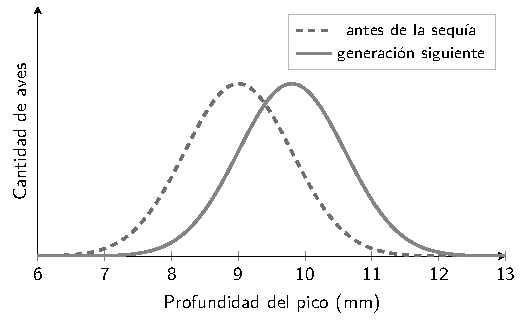
\includegraphics[max width=0.92\linewidth,max height=8.5cm]{bio/evo_pinzones}
\end{center}
\altslargas{Al romper semillas duras, cada ave fortaleció y agrandó su pico, y heredó ese cambio a sus crías.}{Las aves de pico más profundo sobrevivieron y se reprodujeron más durante la sequía, y sus crías heredaron esa característica.}{La sequía causó mutaciones que hicieron crecer el pico de todas las aves de la isla.}{Las aves necesitaban picos más grandes, por lo que sus crías nacieron con picos más profundos.}
\solucion{\textbf{Paso 1. ¿Qué nos piden?} Explicar con la selección natural por qué la curva se desplazó hacia picos más profundos.

\textbf{Paso 2. Variación previa.} Antes de la sequía ya había aves con picos de distintas profundidades: la curva gris va de unos 7 a unos 11 mm.

\textbf{Paso 3. Presión de selección.} La sequía dejó solo semillas grandes y duras. Las aves de pico profundo podían comerlas: sobrevivieron y se reprodujeron más que las de pico poco profundo.

\textbf{Paso 4. Herencia.} Como la profundidad del pico es heredable, la generación siguiente tuvo más aves de pico profundo: la curva naranja está corrida hacia la derecha.

\textbf{Respuesta:} las aves de pico más profundo sobrevivieron y se reprodujeron más, y sus crías heredaron esa característica.

\textbf{¿Por qué no las otras?} Que el pico de cada ave cambie por el uso no explica nada: un cambio adquirido durante la vida no modifica el ADN de los gametos y no se transmite. Las mutaciones ocurren al azar, no son causadas por la necesidad ni afectan a toda la población a la vez. «Necesitaban picos más grandes» tampoco sirve: la necesidad no produce la variación.

\textbf{\color{cienciaD}Para recordar.} El ambiente no cambia a los individuos: favorece a las variantes que ya existían, y la población cambia.}{B}
\end{elejemplo}
\motivacion{Sobreviven los que mejor se adaptan, y tú te estás adaptando a la PAES tema por tema.}

\chapter{Organismo y ambiente}
%% =====================================================================
%% bio_fotosintesis
\section[Fotosíntesis]{Fotosíntesis}
\modcomun\ \ {\color{gris}\itshape Qué es la fotosíntesis y su ecuación global, el efecto de la luz, el CO\textsubscript{2} y la temperatura (factor limitante), y los experimentos clásicos con Elodea, agua marcada y lugol.\par}
\subsection{Qué es la fotosíntesis}
La \textbf{fotosíntesis} es el proceso en que los organismos \textbf{autótrofos fotosintéticos} (plantas, algas y cianobacterias) usan la \textbf{energía de la luz} para fabricar materia orgánica (glucosa) a partir de materia inorgánica: \textbf{dióxido de carbono} y \textbf{agua}.

 

Su ecuación global es:

 
\begin{center}
\textbf{6 CO\textsubscript{2} + 6 H\textsubscript{2}O \ensuremath{\rightarrow} C\textsubscript{6}H\textsubscript{12}O\textsubscript{6} + 6 O\textsubscript{2}}\par \textcolor{gris}{(con luz y clorofila)}
\end{center}
 
\begin{itemize}
  \item \textbf{Reactantes:} CO\textsubscript{2} (entra a la hoja por los estomas) y H\textsubscript{2}O (sube desde las raíces).
  \item \textbf{Productos:} glucosa, que la planta usa como combustible o guarda como \textbf{almidón}, y O\textsubscript{2}, que se libera al ambiente.
  \item \textbf{Transformación de energía:} la energía luminosa queda guardada como \textbf{energía química} en los enlaces de la glucosa.
\end{itemize}
  
\begin{clave}[{Por qué importa}] Casi toda la energía que circula por los ecosistemas entró por la fotosíntesis. Además, es la principal fuente del O\textsubscript{2} de la atmósfera y saca CO\textsubscript{2} del aire: es la puerta de entrada del carbono a los seres vivos.\end{clave}
 
\begin{clave}[{Recuerda}] En plantas y algas la fotosíntesis ocurre en los \textbf{cloroplastos}, organelos que abundan en las células de las hojas y contienen la \textbf{clorofila}, el pigmento que capta la luz. El O\textsubscript{2} liberado viene del \textbf{agua}; el carbono de la glucosa, del \textbf{CO\textsubscript{2}}.\end{clave}
\subsection{Factores que afectan la tasa fotosintética}
\begin{center}
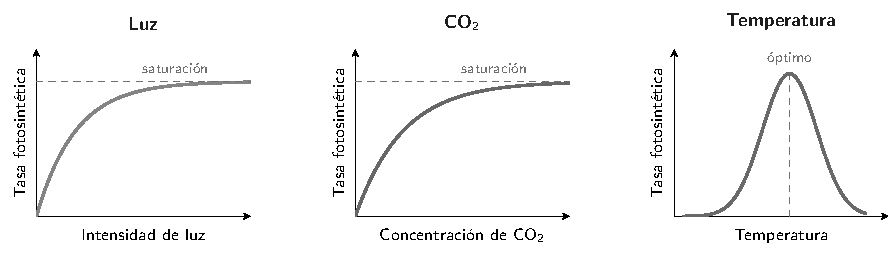
\includegraphics[max width=0.92\linewidth,max height=8.5cm]{bio/amb_factores}
\end{center}
  
\begin{itemize}
  \item \textbf{Intensidad de luz:} al aumentarla, sube la tasa, hasta un punto de \textbf{saturación} en que más luz ya no aumenta la tasa.
  \item \textbf{Concentración de CO\textsubscript{2}:} igual que la luz, sube y se satura.
  \item \textbf{Temperatura:} las enzimas de la fotosíntesis tienen una temperatura \textbf{óptima}. Bajo ella trabajan lento; muy por sobre ella se desnaturalizan y la tasa cae a cero.
\end{itemize}
  
\begin{clave}[{Factor limitante}] Es el factor que está en menor cantidad respecto de lo que se necesita: él fija la tasa, aunque los demás sobren. En la parte que sube de la curva de luz, el limitante es la luz. En la meseta, el limitante es otro factor (CO\textsubscript{2} o temperatura): si se aumenta ese otro factor, la meseta sube.\end{clave}
\subsection{Experimentos clásicos}
\textbf{Elodea y burbujas de O\textsubscript{2}.} Se pone una planta acuática (Elodea) en agua con bicarbonato (fuente de CO\textsubscript{2}) y se ilumina con una lámpara a distintas distancias. Se cuentan las burbujas de O\textsubscript{2} por minuto: a menor distancia (más luz), más burbujas. La distancia de la lámpara es la \textbf{variable independiente}; las burbujas por minuto, la \textbf{dependiente}; la temperatura y el bicarbonato se mantienen \textbf{constantes}.

 

\textbf{Origen del O\textsubscript{2} (agua marcada).} Se usa oxígeno pesado (\textsuperscript{18}O) como marcador. Si se marca el agua, el O\textsubscript{2} liberado sale marcado; si se marca el CO\textsubscript{2}, no. Conclusión: el O\textsubscript{2} de la fotosíntesis viene del \textbf{agua}.

 

\textbf{Almidón y lugol.} El lugol tiñe de azul oscuro el almidón. En una hoja con zonas blancas (sin clorofila), solo las zonas verdes se tiñen: sin clorofila no hay fotosíntesis.

  
\begin{center}
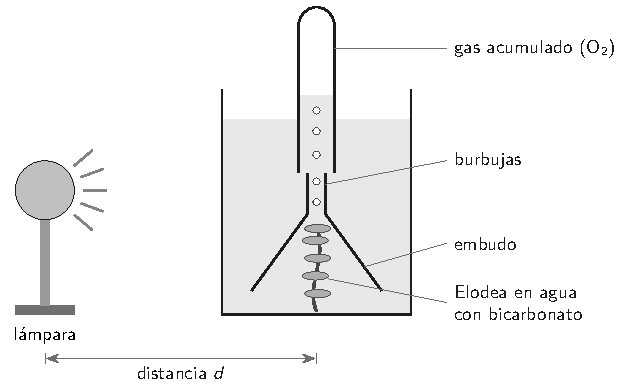
\includegraphics[max width=0.92\linewidth,max height=8.5cm]{bio/amb_elodea}
\end{center}
 
\begin{center}
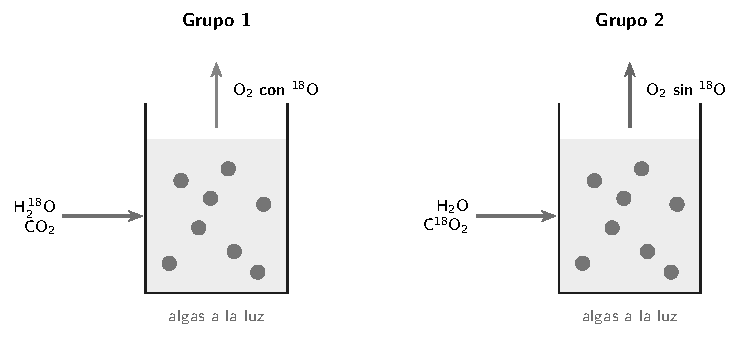
\includegraphics[max width=0.92\linewidth,max height=8.5cm]{bio/amb_isotopos}
\end{center}
\subsection{Lo clave del tema}
\begin{center}\small
\begin{tabularx}{\linewidth}{@{}>{\raggedright\arraybackslash\hsize=0.67\hsize}X>{\raggedright\arraybackslash\hsize=1.33\hsize}X@{}}
\toprule
\textbf{Factor} & \textbf{Efecto sobre la tasa fotosintética} \\
\midrule
Intensidad de luz & sube hasta una saturación \\
Concentración de CO\textsubscript{2} & sube hasta una saturación \\
Temperatura & máxima en el óptimo; baja a ambos lados y se detiene si las enzimas se desnaturalizan \\
\bottomrule
\end{tabularx}
\end{center}
 
\begin{clave}[{Recuerda}] · 6 CO\textsubscript{2} + 6 H\textsubscript{2}O \ensuremath{\rightarrow} C\textsubscript{6}H\textsubscript{12}O\textsubscript{6} + 6 O\textsubscript{2}, con luz y clorofila.\par · El O\textsubscript{2} liberado viene del agua; el carbono de la glucosa, del CO\textsubscript{2}.\par · La glucosa se usa como combustible o se guarda como almidón, que se detecta con lugol.\par · Luz y CO\textsubscript{2} aumentan la tasa hasta una saturación; la temperatura tiene un óptimo.\par · El factor limitante es el que fija la tasa; al aumentarlo, la tasa sube.\end{clave}
 
\begin{clave}[{Método PAES}] 1. Identifica qué mide el experimento (O\textsubscript{2} liberado, CO\textsubscript{2} captado, glucosa o almidón): todos indican cuánta fotosíntesis hubo. 2. Separa la variable independiente (la que se cambia), la dependiente (la que se mide) y las controladas. 3. En un gráfico, busca dónde la curva sube (ese factor limita) y dónde se aplana (limita otro). 4. Revisa cada alternativa contra los datos: no aceptes conclusiones que el experimento no midió.\end{clave}
\begin{elejemplo}{PAES Regular 2026, adaptada}
Un grupo de estudiantes mide la producción de O\textsubscript{2} de una planta acuática a distintas intensidades de luz, con dos concentraciones de CO\textsubscript{2} en el agua y siempre a 25 °C. Sus resultados se muestran en el gráfico:

Con una intensidad de luz de 8 u.a. y CO\textsubscript{2} al 0,03 \%, ¿qué factor limita la producción de O\textsubscript{2}?
\begin{center}
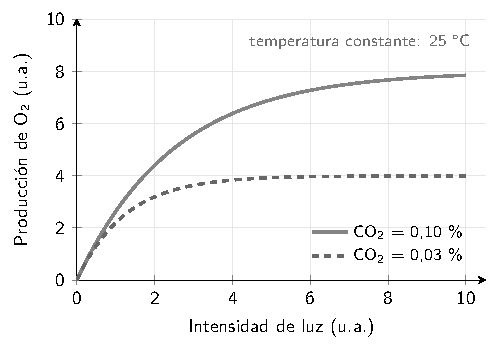
\includegraphics[max width=0.92\linewidth,max height=8.5cm]{bio/amb_limitante}
\end{center}
\alts{La intensidad de luz.}{La concentración de CO\textsubscript{2}.}{La temperatura.}{La cantidad de agua disponible.}
\solucion{\textbf{Paso 1. ¿Qué nos piden?} El factor limitante en un punto del gráfico: el que, si se aumenta, hace subir la producción de O\textsubscript{2}.

\textbf{Paso 2. Mira la curva de CO\textsubscript{2} al 0,03 \%.} Desde una intensidad de 4 u.a. la curva está plana: al pasar de 4 a 8 u.a. de luz la producción se queda en 4 u.a. Más luz no cambia nada, así que la luz ya no limita.

\textbf{Paso 3. Compara con la otra curva.} Con la misma luz (8 u.a.) y la misma temperatura, pero con CO\textsubscript{2} al 0,10 \%, la producción sube a casi 8 u.a. El único factor que cambió fue el CO\textsubscript{2}, y al aumentarlo la producción subió.

\textbf{Respuesta:} la concentración de CO\textsubscript{2} limita la producción en ese punto.

\textbf{¿Por qué no las otras?} La intensidad de luz limita solo en la parte de la curva que sube (bajo 3 u.a. aproximadamente). La temperatura fue la misma, 25 °C, en ambas curvas, así que no explica la diferencia. El agua no fue una variable del experimento: la planta está sumergida.

\textbf{\color{cienciaD}Para recordar.} En la meseta la luz ya no limita: limita el factor que, al aumentarlo, eleva la meseta.}{B}
\end{elejemplo}
\motivacion{Una planta convierte la luz en energía química. Convierte tú este esfuerzo en puntaje.}

%% =====================================================================
%% bio_respiracion
\section[Respiración celular y nutrición]{Respiración celular y nutrición}
\modcomun\ \ {\color{gris}\itshape Nutrición autótrofa y heterótrofa, la respiración celular en la mitocondria (reactantes, productos, ATP y ecuación global), la relación complementaria entre fotosíntesis y respiración y los experimentos con azul de bromotimol y semillas en germinación.\par}
\subsection{Nutrición autótrofa y heterótrofa}
Todo ser vivo necesita materia orgánica: como fuente de \textbf{energía} y como material para \textbf{construir} su cuerpo. Según cómo la obtiene, su nutrición es de dos tipos.

 
\begin{itemize}
  \item \textbf{Autótrofa:} el organismo fabrica su propia materia orgánica a partir de materia inorgánica (CO\textsubscript{2}, agua, sales).\par · \textbf{Fotosintéticos:} usan la energía de la luz (plantas, algas, cianobacterias).\par · \textbf{Quimiosintéticos:} usan la energía de reacciones químicas con sustancias inorgánicas (algunas bacterias de fuentes hidrotermales o del suelo).
  \item \textbf{Heterótrofa:} el organismo obtiene la materia orgánica de otros seres vivos o de sus restos: animales, hongos, la mayoría de las bacterias y muchos protozoos.
\end{itemize}
  
\begin{center}\small
\begin{tabularx}{\linewidth}{@{}>{\raggedright\arraybackslash\hsize=0.78\hsize}X>{\raggedright\arraybackslash\hsize=0.97\hsize}X>{\raggedright\arraybackslash\hsize=1.25\hsize}X@{}}
\toprule
 & \textbf{Autótrofos} & \textbf{Heterótrofos} \\
\midrule
Fuente de carbono & CO\textsubscript{2} & materia orgánica de otros \\
Fuente de energía & luz o reacciones químicas & la materia orgánica que consumen \\
Rol en el ecosistema & productores & consumidores y descomponedores \\
¿Respiran? & sí & sí \\
\bottomrule
\end{tabularx}
\end{center}
 
\begin{clave}[{Recuerda}] Las plantas también respiran, de día y de noche, en todas sus células vivas: la fotosíntesis fabrica la glucosa y la respiración celular la usa para obtener ATP.\end{clave}
\subsection{La respiración celular}
La \textbf{respiración celular aeróbica} degrada la glucosa usando O\textsubscript{2} y guarda parte de su energía en moléculas de \textbf{ATP}, la "moneda energética" de la célula. Ocurre en las células de casi todos los seres vivos, autótrofos y heterótrofos.

 
\begin{center}
\textbf{C\textsubscript{6}H\textsubscript{12}O\textsubscript{6} + 6 O\textsubscript{2} \ensuremath{\rightarrow} 6 CO\textsubscript{2} + 6 H\textsubscript{2}O + energía (ATP y calor)}
\end{center}
 
\begin{itemize}
  \item \textbf{Reactantes:} glucosa y O\textsubscript{2}.
  \item \textbf{Productos:} CO\textsubscript{2}, H\textsubscript{2}O y energía. Parte queda en el ATP (unas 30 a 32 moléculas por glucosa) y el resto se libera como \textbf{calor}.
  \item \textbf{Lugar:} comienza en el citoplasma (glucólisis) y se completa en la \textbf{mitocondria}.
\end{itemize}
  
\begin{center}
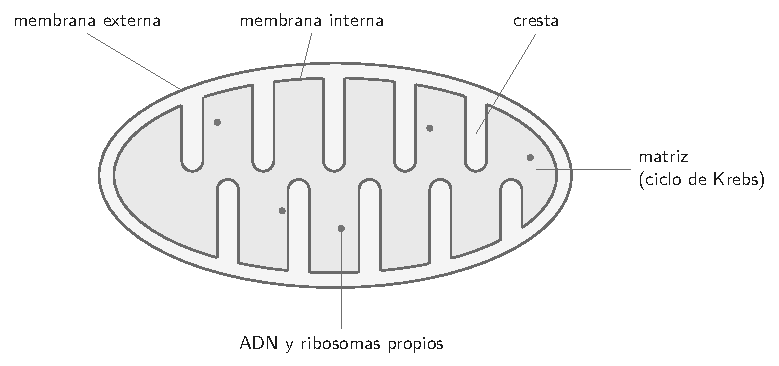
\includegraphics[max width=0.92\linewidth,max height=8.5cm]{bio/amb_mitocondria}
\end{center}
 
\begin{clave}[{Recuerda}] Es un proceso \textbf{catabólico}: rompe una molécula grande (glucosa) en moléculas pequeñas (CO\textsubscript{2} y H\textsubscript{2}O) y libera energía.\end{clave}
\subsection{Las etapas, en resumen}
\begin{center}\small
\begin{tabularx}{\linewidth}{@{}>{\raggedright\arraybackslash\hsize=1.11\hsize}X>{\raggedright\arraybackslash\hsize=0.74\hsize}X>{\raggedright\arraybackslash\hsize=1.14\hsize}X@{}}
\toprule
\textbf{Etapa} & \textbf{Lugar} & \textbf{Qué pasa} \\
\midrule
Glucólisis & citoplasma & la glucosa se divide en dos moléculas de piruvato; se forman 2 ATP \\
Ciclo de Krebs & matriz mitocondrial & el piruvato se oxida por completo; se libera \textbf{CO\textsubscript{2}} \\
Cadena transportadora y síntesis de ATP & membrana interna (crestas) & el \textbf{O\textsubscript{2}} recibe los electrones y forma \textbf{H\textsubscript{2}O}; se produce la mayor parte del ATP \\
\bottomrule
\end{tabularx}
\end{center}
  
\begin{clave}[{¿De dónde viene y a dónde va cada cosa?}] · El CO\textsubscript{2} que exhalas se forma en la \textbf{matriz} (ciclo de Krebs).\par · El O\textsubscript{2} que inhalas se usa al final, en las \textbf{crestas}, y termina formando agua.\end{clave}
 
\begin{clave}[{Sin oxígeno}] Algunas células, como las levaduras o las musculares en ejercicio intenso, pueden obtener energía sin O\textsubscript{2} por \textbf{fermentación}. Rinde solo 2 ATP por glucosa, mucho menos que la respiración aeróbica.\end{clave}
\subsection{Fotosíntesis y respiración: procesos complementarios}
\begin{center}
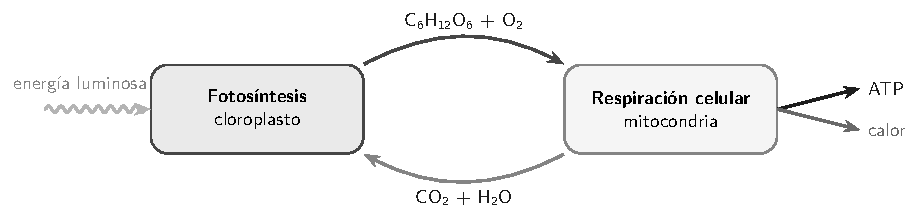
\includegraphics[max width=0.92\linewidth,max height=8.5cm]{bio/amb_complemento}
\end{center}
 
\begin{center}\small
\begin{tabularx}{\linewidth}{@{}>{\raggedright\arraybackslash\hsize=0.42\hsize}X>{\raggedright\arraybackslash\hsize=1.29\hsize}X>{\raggedright\arraybackslash\hsize=1.29\hsize}X@{}}
\toprule
 & \textbf{Fotosíntesis} & \textbf{Respiración celular} \\
\midrule
Organelo & cloroplasto & mitocondria (y citoplasma) \\
Organismos & autótrofos fotosintéticos & autótrofos y heterótrofos \\
Reactantes & CO\textsubscript{2} y H\textsubscript{2}O (más luz) & glucosa y O\textsubscript{2} \\
Productos & glucosa y O\textsubscript{2} & CO\textsubscript{2}, H\textsubscript{2}O y ATP \\
Energía & la luz queda guardada como energía química & la energía química se libera como ATP y calor \\
Cuándo & solo con luz & siempre, de día y de noche \\
\bottomrule
\end{tabularx}
\end{center}
 
\begin{clave}[{La idea clave}] Los productos de una son los reactantes de la otra. La materia (C, H, O) circula entre ambos procesos; la energía no: entra como luz y sale como calor.\end{clave}
\subsection{Experimentos con indicadores}
El \textbf{azul de bromotimol} es un indicador de pH. El CO\textsubscript{2} disuelto en agua forma ácido carbónico y baja el pH.

 
\begin{itemize}
  \item \textbf{Azul:} poco CO\textsubscript{2} (se consumió CO\textsubscript{2}).
  \item \textbf{Verde:} nivel intermedio.
  \item \textbf{Amarillo:} mucho CO\textsubscript{2} (se liberó CO\textsubscript{2}).
\end{itemize}
 

En los tubos de la figura, todos parten verdes. La Elodea a la luz hace más fotosíntesis que respiración y saca CO\textsubscript{2}: el tubo se vuelve azul. En la oscuridad solo respira y el tubo se vuelve amarillo, igual que con el caracol. El tubo sin organismos es el \textbf{control}: muestra que el color no cambia solo.

  
\begin{center}
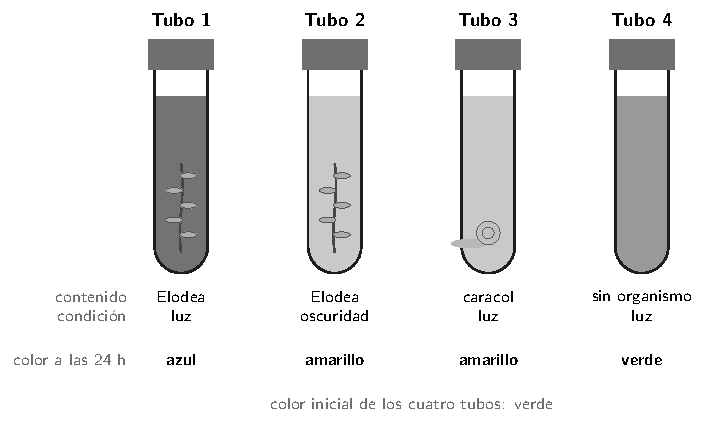
\includegraphics[max width=0.92\linewidth,max height=8.5cm]{bio/amb_tubos_abt}
\end{center}
   

\textbf{Semillas en germinación.} Una semilla que germina respira con mucha intensidad: usa sus reservas, libera CO\textsubscript{2} y desprende calor. Si se comparan con semillas hervidas (muertas), solo en el frasco de las semillas vivas sube la temperatura y el indicador se pone amarillo.

  
\begin{center}
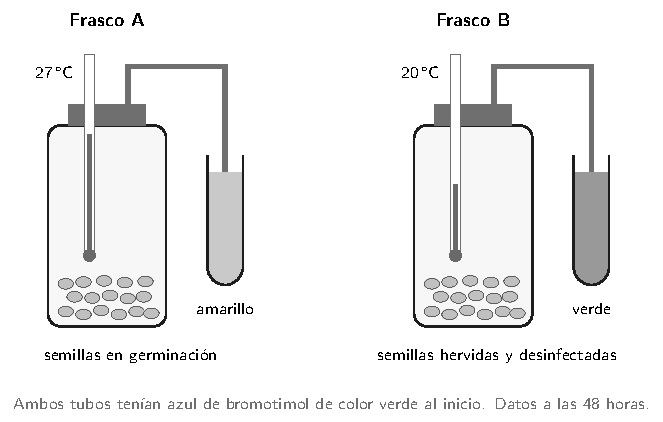
\includegraphics[max width=0.92\linewidth,max height=8.5cm]{bio/amb_semillas}
\end{center}
\subsection{Lo clave del tema}
\begin{center}\small
\begin{tabularx}{\linewidth}{@{}>{\raggedright\arraybackslash\hsize=0.69\hsize}X>{\raggedright\arraybackslash\hsize=1.31\hsize}X@{}}
\toprule
\textbf{Concepto} & \textbf{Idea central} \\
\midrule
Nutrición autótrofa & fabrica materia orgánica desde CO\textsubscript{2} (con luz o energía química) \\
Nutrición heterótrofa & obtiene la materia orgánica de otros seres vivos \\
Respiración celular & glucosa + O\textsubscript{2} \ensuremath{\rightarrow} CO\textsubscript{2} + H\textsubscript{2}O + ATP y calor; en la mitocondria \\
Azul de bromotimol & amarillo = más CO\textsubscript{2}; azul = menos CO\textsubscript{2} \\
\bottomrule
\end{tabularx}
\end{center}
 
\begin{clave}[{Recuerda}] · Autótrofos y heterótrofos respiran; las plantas respiran de día y de noche.\par · El CO\textsubscript{2} de la respiración se forma en la matriz; el O\textsubscript{2} se usa en las crestas y forma agua.\par · Los productos de la fotosíntesis son los reactantes de la respiración, y viceversa.\end{clave}
 
\begin{clave}[{Método PAES}] 1. Anota qué proceso puede ocurrir en cada condición: con luz, fotosíntesis y respiración; sin luz, solo respiración; en animales y semillas, solo respiración. 2. Decide cuál predomina y qué gas se acumula. 3. Traduce a la medición: más CO\textsubscript{2} \ensuremath{\rightarrow} indicador amarillo; menos CO\textsubscript{2} \ensuremath{\rightarrow} azul; más respiración \ensuremath{\rightarrow} más calor. 4. Busca el control: el tubo o frasco que muestra qué pasa sin el factor estudiado.\end{clave}
\begin{elejemplo}{PAES Invierno 2027, adaptada}
Una profesora prepara cuatro tubos con azul de bromotimol, todos de color verde al inicio, y los tapa. El indicador se vuelve amarillo cuando aumenta el CO\textsubscript{2} disuelto y azul cuando disminuye. Después de 24 horas observa los colores que muestra la figura:

¿Cuál conclusión es correcta?
\begin{center}
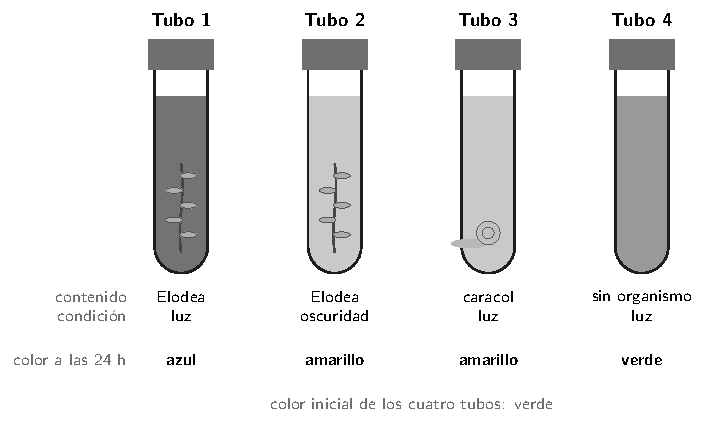
\includegraphics[max width=0.92\linewidth,max height=8.5cm]{bio/amb_tubos_abt}
\end{center}
\altslargas{En el tubo 1, la Elodea consumió más CO\textsubscript{2} del que liberó.}{En el tubo 2, la Elodea hizo fotosíntesis, pero no respiró.}{En el tubo 3, el caracol consumió el CO\textsubscript{2} disuelto.}{El tubo 4 muestra que la luz, por sí sola, vuelve azul el indicador.}
\solucion{\textbf{Paso 1. ¿Qué nos piden?} Interpretar cada color según el CO\textsubscript{2}: azul = bajó, amarillo = subió, verde = no cambió.

\textbf{Paso 2. Tubo 1 (Elodea, luz): azul.} El CO\textsubscript{2} bajó. La planta respira y libera CO\textsubscript{2}, pero a la luz también hace fotosíntesis, que lo consume. Como bajó, consumió más del que liberó.

\textbf{Paso 3. Los demás.} Tubo 2 (oscuridad): amarillo; sin luz no hay fotosíntesis y la respiración liberó CO\textsubscript{2}. Tubo 3: el caracol respira y liberó CO\textsubscript{2}. Tubo 4: sin organismos, el color no cambió.

\textbf{Respuesta:} en el tubo 1, la Elodea consumió más CO\textsubscript{2} del que liberó.

\textbf{¿Por qué no las otras?} En el tubo 2 ocurrió lo contrario: sin luz no hay fotosíntesis, y la planta siguió respirando. El caracol no hace fotosíntesis: libera CO\textsubscript{2} y por eso su tubo se puso amarillo. El tubo 4 recibió luz y quedó verde: la luz sola no cambia el color.

\textbf{\color{cienciaD}Para recordar.} Azul = se consumió CO\textsubscript{2} (fotosíntesis mayor que respiración); amarillo = se liberó CO\textsubscript{2} (respiración).}{A}
\end{elejemplo}
\motivacion{Glucosa y oxígeno: así sacan energía tus células para estudiar. Come bien, respira hondo y sigue.}

%% =====================================================================
%% bio_flujo
\section[Flujo de energía y ciclos del carbono y del oxígeno]{Flujo de energía y ciclos del carbono y del oxígeno}
\modcomun\ \ {\color{gris}\itshape Productores, consumidores y descomponedores; cadenas y tramas tróficas; flujo unidireccional de la energía con pérdida de cerca del 90 \% en cada nivel; pirámides ecológicas; ciclos del carbono y del oxígeno, el rol de la fotosíntesis y la respiración, y el efecto de la combustión y la deforestación.\par}
\subsection{Niveles tróficos}
En un ecosistema, cada organismo ocupa un \textbf{nivel trófico} según cómo obtiene su materia orgánica.

 
\begin{itemize}
  \item \textbf{Productores} (autótrofos): plantas, algas, fitoplancton y cianobacterias. Fabrican materia orgánica por fotosíntesis. Son la puerta de entrada de la energía y del carbono.
  \item \textbf{Consumidores} (heterótrofos): se alimentan de otros seres vivos.\par · \textbf{Primarios} (herbívoros): comen productores.\par · \textbf{Secundarios}: comen consumidores primarios.\par · \textbf{Terciarios}: comen consumidores secundarios.
  \item \textbf{Descomponedores} (hongos y bacterias): degradan restos, desechos y cadáveres de todos los niveles. Devuelven al ambiente el CO\textsubscript{2} y los minerales que los productores vuelven a usar.
\end{itemize}
  
\begin{clave}[{Cadena trófica}] Una secuencia lineal de quién come a quién. Las flechas van desde el alimento hacia quien lo come, porque indican hacia dónde va la energía.\par pasto \ensuremath{\rightarrow} degú \ensuremath{\rightarrow} culebra de cola larga \ensuremath{\rightarrow} águila mora\end{clave}
 
\begin{clave}[{Recuerda}] Un mismo organismo puede ocupar más de un nivel trófico si se alimenta de presas de niveles distintos.\end{clave}
\subsection{Tramas tróficas}
En la naturaleza las cadenas se entrecruzan: casi todos los organismos tienen varias presas y varios depredadores. El conjunto de cadenas conectadas es una \textbf{trama trófica}.

 

En la trama marina de la figura, el lobo marino come jibias y anchovetas: es consumidor \textbf{cuaternario} en una cadena y \textbf{terciario} en otra.

 

\textbf{Para analizar una trama:}

 
\begin{itemize}
  \item Para contar cadenas, parte en cada productor y sigue todas las flechas hasta llegar a un organismo que nadie come.
  \item Si una especie desaparece, sus depredadores pierden alimento (y bajan, salvo que tengan otras presas) y sus presas pierden un depredador (y pueden aumentar).
\end{itemize}
  
\begin{center}
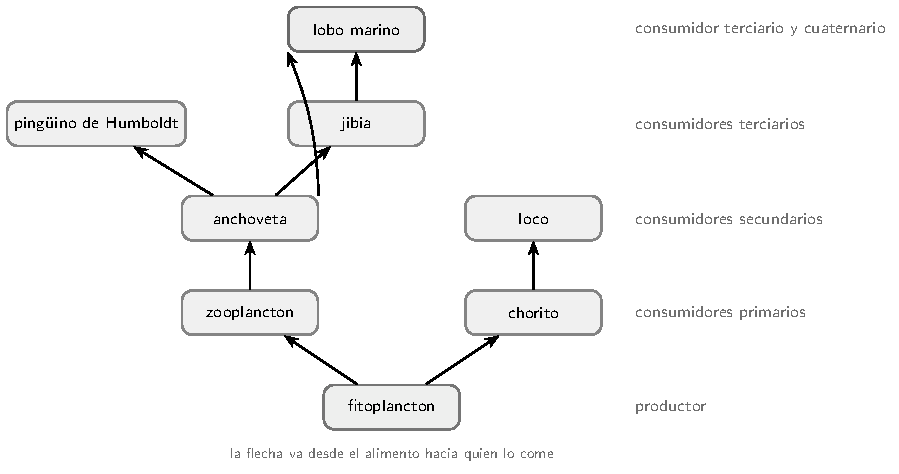
\includegraphics[max width=0.92\linewidth,max height=8.5cm]{bio/amb_trama}
\end{center}
\subsection{El flujo de energía}
\begin{center}
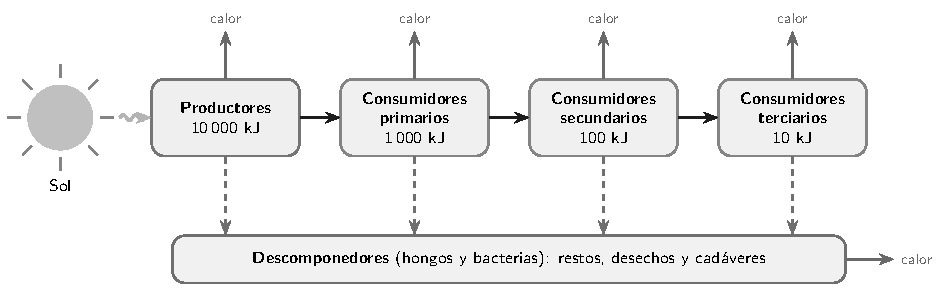
\includegraphics[max width=0.92\linewidth,max height=8.5cm]{bio/amb_flujo_energia}
\end{center}
  
\begin{itemize}
  \item La energía entra como \textbf{luz}, los productores la transforman en \textbf{energía química} y pasa de nivel en nivel con el alimento.
  \item En cada nivel, la mayor parte de la energía se usa en la \textbf{respiración celular} (moverse, mantener la temperatura, crecer) y se pierde como \textbf{calor}. Otra parte no se come o no se digiere y va a los descomponedores.
  \item Solo cerca del \textbf{10 \%} de la energía de un nivel queda en el siguiente.
\end{itemize}
  
\begin{clave}[{Recuerda}] El flujo de energía es \textbf{unidireccional}: el calor no se puede volver a usar para la fotosíntesis. Por eso los ecosistemas necesitan un aporte constante de luz solar. La materia, en cambio, se recicla.\end{clave}
 
\begin{clave}[{Consecuencia}] Las cadenas tróficas son cortas (rara vez más de 4 o 5 niveles): arriba queda muy poca energía.\end{clave}
\subsection{Pirámides ecológicas}
\begin{center}
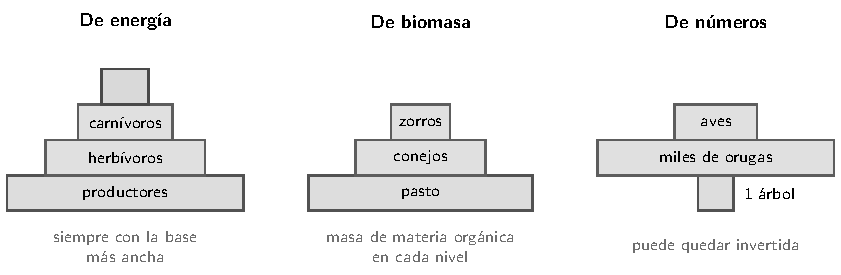
\includegraphics[max width=0.92\linewidth,max height=8.5cm]{bio/amb_piramides}
\end{center}
  
\begin{itemize}
  \item \textbf{De energía:} la energía de cada nivel en un tiempo dado. \textbf{Siempre} tiene la base más ancha, porque en cada paso se pierde energía como calor.
  \item \textbf{De biomasa:} la masa de materia orgánica de cada nivel. Suele tener la base ancha, aunque en algunos ecosistemas acuáticos se invierte (el fitoplancton se reproduce tan rápido que su masa en un momento es menor que la del zooplancton).
  \item \textbf{De números:} la cantidad de individuos. Puede invertirse cuando un productor grande alimenta a muchos consumidores pequeños, como un árbol con miles de orugas.
\end{itemize}
  
\begin{clave}[{Recuerda}] De las tres, solo la pirámide de energía nunca se invierte.\end{clave}
\subsection{El ciclo del carbono}
\begin{center}
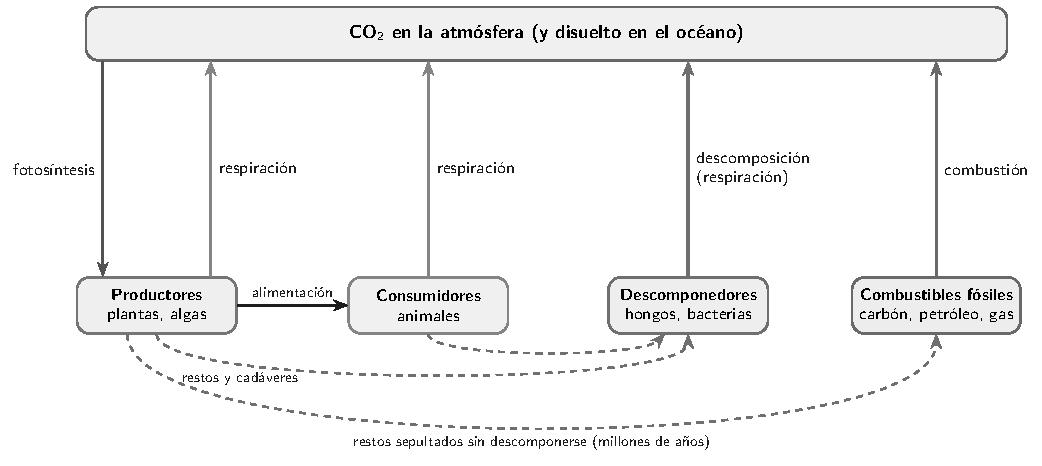
\includegraphics[max width=0.92\linewidth,max height=8.5cm]{bio/amb_ciclo_carbono}
\end{center}
  
\begin{itemize}
  \item \textbf{Entrada a los seres vivos:} la \textbf{fotosíntesis} fija el CO\textsubscript{2} del aire (o disuelto en el agua) en moléculas orgánicas.
  \item \textbf{Paso por la trama:} el carbono pasa a los consumidores con el alimento y a los descomponedores con los restos.
  \item \textbf{Regreso a la atmósfera:} la \textbf{respiración celular} de todos los seres vivos, incluida la de los descomponedores, y la \textbf{combustión}.
  \item \textbf{Reservas lentas:} restos sepultados sin descomponerse, durante millones de años, formaron carbón, petróleo y gas natural.
\end{itemize}
  
\begin{clave}[{Recuerda}] Fotosíntesis y respiración son las dos caras del ciclo: una saca CO\textsubscript{2} de la atmósfera y la otra lo devuelve. A diferencia de la energía, el carbono se recicla una y otra vez.\end{clave}
\subsection{Ciclo del oxígeno y acción humana}
\textbf{Ciclo del oxígeno.} Va unido al del carbono. La \textbf{fotosíntesis} libera O\textsubscript{2} (que viene del agua). La \textbf{respiración celular} y la \textbf{combustión} consumen O\textsubscript{2} y forman CO\textsubscript{2} y agua. Ese CO\textsubscript{2} y esa agua vuelven a usarse en la fotosíntesis.

 

\textbf{Combustión de combustibles fósiles.} Libera en pocos años carbono que estuvo guardado millones de años: aumenta el CO\textsubscript{2} de la atmósfera.

 

\textbf{Deforestación.} Aumenta el CO\textsubscript{2} por dos vías: si el bosque se quema, su carbono pasa al aire como CO\textsubscript{2}; y sin los árboles, se fija menos CO\textsubscript{2} por fotosíntesis.

 

El CO\textsubscript{2} es un gas de efecto invernadero: su aumento intensifica el calentamiento global.

  
\begin{center}
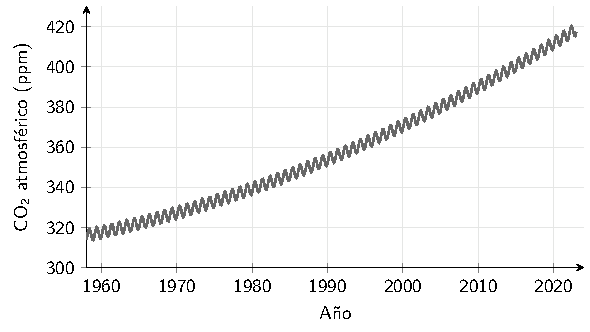
\includegraphics[max width=0.92\linewidth,max height=8.5cm]{bio/amb_keeling}
\end{center}
 
\begin{clave}[{Cómo leer la curva}] La tendencia que sube se debe sobre todo a la quema de combustibles fósiles y a la deforestación. La pequeña oscilación anual se debe a la fotosíntesis: en el verano del hemisferio norte, donde hay más bosques, el CO\textsubscript{2} baja; en su invierno, sube.\end{clave}
\subsection{Lo clave del tema}
\begin{center}\small
\begin{tabularx}{\linewidth}{@{}>{\raggedright\arraybackslash\hsize=0.50\hsize}X>{\raggedright\arraybackslash\hsize=1.25\hsize}X>{\raggedright\arraybackslash\hsize=1.25\hsize}X@{}}
\toprule
 & \textbf{Energía} & \textbf{Materia (C y O)} \\
\midrule
Recorrido & unidireccional: luz \ensuremath{\rightarrow} energía química \ensuremath{\rightarrow} calor & cíclico: se recicla \\
Entrada & fotosíntesis (luz) & fotosíntesis (fija CO\textsubscript{2} y libera O\textsubscript{2}) \\
Salida o retorno & calor de la respiración en cada nivel & respiración, descomposición y combustión devuelven CO\textsubscript{2} \\
En cada nivel & queda cerca del 10 \% & pasa con el alimento y los restos \\
\bottomrule
\end{tabularx}
\end{center}
 
\begin{clave}[{Recuerda}] · Las flechas de una trama van del alimento hacia quien lo come.\par · La pirámide de energía siempre tiene la base más ancha.\par · Los descomponedores devuelven materia, no energía, a los productores.\par · La combustión y la deforestación aumentan el CO\textsubscript{2} atmosférico.\end{clave}
 
\begin{clave}[{Método PAES}] 1. En una trama, ubica a los productores y sigue las flechas para asignar niveles. 2. Para calcular energía, multiplica por 0,1 en cada paso hacia arriba (o por 10 hacia abajo). 3. En un ciclo, separa los procesos que sacan CO\textsubscript{2} del aire (fotosíntesis) de los que lo devuelven (respiración, descomposición, combustión). 4. En tablas de datos, describe solo la tendencia que muestran los números.\end{clave}
\begin{elejemplo}{Estilo PAES}
El esquema muestra una cadena trófica de una pradera y la energía que contiene cada nivel en un año:

Si en cada nivel queda cerca del 10 \% de la energía del nivel anterior, ¿cuánta energía llega aproximadamente al cernícalo?
\begin{center}
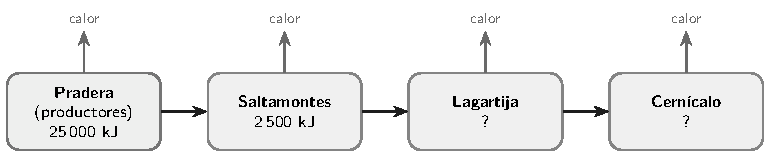
\includegraphics[max width=0.92\linewidth,max height=8.5cm]{bio/amb_energia_q}
\end{center}
\alts{2 500 kJ}{250 kJ}{25 kJ}{2,5 kJ}
\solucion{\textbf{Paso 1. ¿Qué nos piden?} La energía del cuarto nivel (cernícalo), sabiendo que pasa cerca del 10 \% de un nivel al siguiente.

\textbf{Paso 2. Comprueba la regla con los datos.} De la pradera (25 000 kJ) a los saltamontes (2 500 kJ) pasa el 10 \%. Se cumple.

\textbf{Paso 3. Sigue la cadena.} Lagartija: 10 \% de 2 500 = 250 kJ. Cernícalo: 10 \% de 250 = 25 kJ.

\textbf{Respuesta:} 25 kJ.

\textbf{¿Por qué no las otras?} 2 500 kJ es la energía de los saltamontes. 250 kJ es la de la lagartija: falta un paso. 2,5 kJ supone un paso de más, como si hubiera un quinto nivel.

\textbf{\color{cienciaD}Para recordar.} Cada paso hacia arriba en la cadena multiplica la energía por cerca de 0,1.}{C}
\end{elejemplo}
\motivacion{La energía fluye y la materia circula. Tu aprendizaje también fluye: ya casi terminas Biología.}

\chapter{Habilidades científicas}
%% =====================================================================
%% bio_hab_investigacion
\section[Preguntas, hipótesis y variables]{Preguntas, hipótesis y variables}
\modcomun\ \ {\color{gris}\itshape Cómo se arma una investigación en biología: pregunta investigable, hipótesis y predicción, variables independiente, dependiente y controladas, grupo control, componentes de una investigación (teoría, ley, modelo, objetivo, resultado, inferencia, conclusión) y un procedimiento que cambie solo una variable.\par}
\subsection{La investigación científica paso a paso}
Entre un cuarto y un tercio de las preguntas de la PAES de Ciencias no miden cuánta biología sabes, sino si sabes \textbf{pensar como investigador}: reconocer la pregunta, la hipótesis, las variables y la conclusión de un estudio. Todas siguen el mismo esquema:

 
\begin{center}
\includegraphics[max width=0.92\linewidth,max height=8.5cm]{bio/hab_ciclo}
\end{center}
  

\textbf{Un ejemplo completo.}

 

\textbf{1. Observación.} Una estudiante nota que las semillas de rabanito brotan antes en primavera que en invierno.

 

\textbf{2. Pregunta.} ¿Cómo influye la temperatura en la germinación de las semillas de rabanito?

 

\textbf{3. Hipótesis.} La temperatura influye en el porcentaje de semillas que germinan.

 

\textbf{4. Predicción.} Si la hipótesis es correcta, a 20 °C germinará un porcentaje distinto de semillas que a 10 °C.

 

\textbf{5. Procedimiento.} Pone 10 semillas en placas con papel húmedo a 10, 20, 30 y 40 °C, y después de 4 días cuenta las semillas germinadas.

 

\textbf{6. Resultados.} 20 \%, 70 \%, 90 \% y 30 \%.

 

\textbf{7. Conclusión.} En el rango estudiado, la temperatura influyó en la germinación: el mayor porcentaje se obtuvo a 30 °C.

  
\begin{clave}[{Pregunta investigable}] Es una pregunta que se puede responder \textbf{midiendo} u observando algo. Casi siempre relaciona dos variables: «¿cómo influye A en B?».\end{clave}
 
\begin{clave}[{¿Investigable o no?}] · «¿Influye la cantidad de luz en el crecimiento de una planta de poroto?»: sí, se mide la altura.\par · «¿Es el colibrí el ave más hermosa de Chile?»: no, es una opinión.\par · «¿Qué especies existirán dentro de un millón de años?»: no, no se puede medir hoy.\end{clave}
 
\begin{clave}[{Recuerda}] La pregunta de investigación calza con los datos. Si en la tabla solo cambia la especie de planta y se mide la altura, la pregunta es «¿cómo varía la altura entre estas especies?».\end{clave}
\subsection{Hipótesis y predicción}
La \textbf{hipótesis} es una explicación o respuesta tentativa a la pregunta. Tiene tres rasgos:

 
\begin{itemize}
  \item Se escribe \textbf{antes} del experimento.
  \item Relaciona la variable que se cambia con la que se mide: «la temperatura influye en la actividad de la levadura», «a mayor intensidad de luz, mayor tasa de fotosíntesis».
  \item Se puede poner a prueba, y podría resultar falsa.
\end{itemize}
 

La \textbf{predicción} es más concreta: dice qué resultado se espera en \textbf{este} experimento si la hipótesis es cierta. Suele tener la forma «si\dots{}, entonces\dots{}».

 
\begin{center}\small
\begin{tabularx}{\linewidth}{@{}>{\raggedright\arraybackslash\hsize=1.00\hsize}X>{\raggedright\arraybackslash\hsize=1.00\hsize}X@{}}
\toprule
\textbf{Hipótesis} & \textbf{Predicción} \\
\midrule
La intensidad de luz influye en la tasa de fotosíntesis de \emph{Elodea}. & Con la lámpara a 10 cm, la rama liberará más burbujas por minuto que con la lámpara a 40 cm. \\
La temperatura influye en la producción de CO\textsubscript{2} de la levadura. & El globo del matraz a 35 °C se inflará más que el del matraz a 10 °C. \\
\bottomrule
\end{tabularx}
\end{center}
  
\begin{ejemplo}[{Ejemplo resuelto: ¿qué hipótesis se puso a prueba?}] Unos estudiantes riegan cuatro grupos de plantas de lechuga con agua que tiene 0, 1, 2 y 4 g/L de sal. Todas son de la misma edad, están en el mismo invernadero y reciben el mismo volumen de agua. Después de 3 semanas miden la masa de cada planta.\par \textbf{Paso 1.} ¿Qué cambia de un grupo a otro? Solo la concentración de sal del agua de riego.\par \textbf{Paso 2.} ¿Qué se mide? La masa de las plantas.\par \textbf{Paso 3.} La hipótesis une las dos: «la concentración de sal del agua de riego influye en el crecimiento de la lechuga».\par Una hipótesis sobre la luz, la edad de las plantas o el volumen de riego no se puede probar aquí: esas variables se mantuvieron iguales.\end{ejemplo}
 
\begin{clave}[{Recuerda}] La hipótesis va antes de experimentar; la conclusión, después, apoyada en los datos. Un experimento no «demuestra» una hipótesis para siempre: la apoya o la contradice.\end{clave}
\subsection{Variables: independiente, dependiente y controladas}
\begin{center}
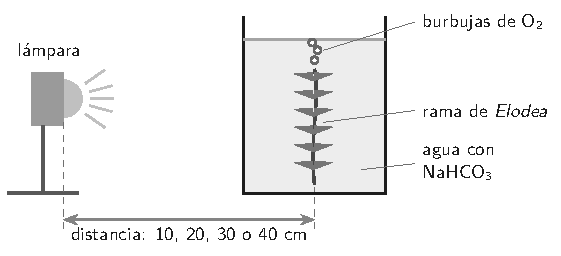
\includegraphics[max width=0.92\linewidth,max height=8.5cm]{bio/hab_elodea}
\end{center}
  

En el montaje, un grupo pone una rama de \emph{Elodea} (planta acuática) en agua con bicarbonato de sodio, que aporta CO\textsubscript{2}. Ubica la lámpara a distintas distancias y cuenta las burbujas de O\textsubscript{2} que libera la rama en un minuto.

 
\begin{center}\small
\begin{tabularx}{\linewidth}{@{}>{\raggedright\arraybackslash\hsize=0.50\hsize}X>{\raggedright\arraybackslash\hsize=1.25\hsize}X>{\raggedright\arraybackslash\hsize=1.25\hsize}X@{}}
\toprule
\textbf{Variable} & \textbf{Cómo reconocerla} & \textbf{En el montaje} \\
\midrule
\textbf{Independiente} & La que el investigador \textbf{cambia a propósito} (la causa). & Distancia de la lámpara, es decir, la intensidad de luz \\
\textbf{Dependiente} & La que se \textbf{mide} como respuesta (el efecto). & Burbujas de O\textsubscript{2} por minuto \\
\textbf{Controladas} & Las que se dejan \textbf{iguales} para que no influyan. & Rama de la misma planta, temperatura del agua, cantidad de bicarbonato, tiempo de conteo \\
\bottomrule
\end{tabularx}
\end{center}
  
\gatotip[\gatogris]{\textbf{Truco de la frase.} Arma la frase «el efecto de \textbf{[independiente]} sobre \textbf{[dependiente]}». Aquí: «el efecto de la intensidad de luz sobre la liberación de O\textsubscript{2}». Si la frase no tiene sentido, cambiaste el orden.}
 
\begin{ejemplo}[{Ejemplo resuelto}] Se cultivan bacterias en placas con 0, 5, 10 y 20 mg/L de un antibiótico, todas a 37 °C, y después de 24 h se cuentan las colonias.\par · Cambia a propósito: la concentración de antibiótico \ensuremath{\rightarrow} \textbf{independiente}.\par · Se mide al final: el número de colonias \ensuremath{\rightarrow} \textbf{dependiente}.\par · Siempre igual: la temperatura (37 °C) y el tiempo (24 h) \ensuremath{\rightarrow} \textbf{controladas}.\end{ejemplo}
 
\begin{clave}[{Recuerda}] Para encontrar la variable independiente, pregúntate qué decidió el investigador \textbf{antes} de medir. La dependiente es lo que registra al final, muchas veces con un instrumento.\end{clave}
\subsection{Grupo control, comparaciones justas e instrumentos}
El \textbf{grupo control} es el grupo de comparación: igual a los demás, pero \textbf{sin} el factor que se estudia. Si quieres probar que un fertilizante aumenta el crecimiento del tomate, necesitas plantas con fertilizante y otras plantas iguales, con el mismo riego, luz y suelo, pero sin fertilizante. Sin ese grupo no sabes si el fertilizante hizo algo.

 

En los estudios con personas, el grupo control suele recibir un \textbf{placebo}: una pastilla igual, pero sin el fármaco, para que la sola idea de estar tratado no influya en el resultado.

 

\textbf{Compara solo grupos que se diferencian en una cosa.}

 
\begin{center}\small
\begin{tabular}{@{}lll@{}}
\toprule
\textbf{Grupo} & \textbf{Temperatura} & \textbf{Luz} \\
\midrule
1 & 20 °C & 12 h/día \\
2 & 30 °C & 12 h/día \\
3 & 30 °C & 16 h/día \\
\bottomrule
\end{tabular}
\end{center}
 

· 1 y 2: solo cambia la temperatura \ensuremath{\rightarrow} sirven para estudiar la temperatura.\par · 2 y 3: solo cambian las horas de luz \ensuremath{\rightarrow} sirven para estudiar la luz.\par · 1 y 3: cambian dos cosas \ensuremath{\rightarrow} no permiten saber cuál causó la diferencia.

  
\begin{clave}[{Instrumentos según la variable}] \begin{center}\small
\begin{tabularx}{\linewidth}{@{}>{\raggedright\arraybackslash\hsize=1.00\hsize}X>{\raggedright\arraybackslash\hsize=1.00\hsize}X@{}}
\toprule
\textbf{Para medir\dots{}} & \textbf{se usa\dots{}} \\
\midrule
masa (de una planta, de una semilla) & balanza \\
longitud (altura de un tallo, largo de una raíz) & regla o huincha \\
volumen de un líquido & probeta o pipeta \\
volumen de un gas (CO\textsubscript{2}, O\textsubscript{2}) & jeringa o probeta invertida \\
temperatura & termómetro \\
tiempo & cronómetro \\
acidez & pHmetro o papel indicador \\
frecuencia cardíaca & pulsómetro, o contar el pulso con un cronómetro \\
células, estructuras pequeñas & microscopio \\
\bottomrule
\end{tabularx}
\end{center}\end{clave}
 
\begin{clave}[{Recuerda}] Antes de elegir un instrumento, identifica qué variable piden. Si se calienta un cultivo y se cuentan sus colonias, el termómetro mide la variable independiente y el conteo de colonias es la dependiente.\end{clave}
\subsection{Teoría, ley, modelo y los demás componentes}
La PAES pregunta mucho «¿a qué componente de la investigación corresponde la frase entre comillas?». Apréndete esta tabla:

 
\begin{center}\small
\begin{tabularx}{\linewidth}{@{}>{\raggedright\arraybackslash\hsize=0.62\hsize}X>{\raggedright\arraybackslash\hsize=1.19\hsize}X>{\raggedright\arraybackslash\hsize=1.19\hsize}X@{}}
\toprule
\textbf{Componente} & \textbf{Qué es} & \textbf{Ejemplo en biología} \\
\midrule
\textbf{Teoría} & Explica \textbf{por qué} pasa algo; está respaldada por mucha evidencia. & Teoría celular; teoría de la evolución por selección natural. \\
\textbf{Ley} & Describe una regularidad: \textbf{qué} pasa, sin explicar por qué. & Leyes de Mendel (segregación, distribución independiente). \\
\textbf{Modelo} & Representación simplificada para explicar o predecir. & Modelo del mosaico fluido de la membrana; modelo de doble hélice del ADN; modelo llave-cerradura de las enzimas. \\
\textbf{Marco conceptual} & Lo que ya se sabe del tema: teorías, leyes, modelos y antecedentes. & «La insulina disminuye la glucosa en la sangre». \\
\textbf{Problema / pregunta} & Lo que se quiere averiguar. & «¿Cómo afecta la sal del suelo al crecimiento de la lechuga?». \\
\textbf{Objetivo} & Lo que se quiere lograr; empieza con un verbo en infinitivo. & «Determinar el efecto de la temperatura en la germinación del trigo». \\
\textbf{Procedimiento} & Los pasos que se siguen. & «Se sembraron 10 semillas por placa y se incubaron a 20 °C\dots{}». \\
\textbf{Resultado / evidencia} & Los datos obtenidos. & «Germinaron 9 de 10 semillas a 30 °C». \\
\textbf{Inferencia} & Interpretación que va más allá de lo observado. & «Las guarderías de polluelos podrían aumentar su sobrevivencia». \\
\textbf{Conclusión} & Respuesta a la pregunta, apoyada en los resultados. & «En el rango estudiado, la germinación fue máxima a 30 °C». \\
\bottomrule
\end{tabularx}
\end{center}
  
\begin{clave}[{Pistas en el texto}] · «si\dots{}, entonces\dots{} ocurrirá»: predicción.\par · «determinar», «evaluar», «comparar», en infinitivo: objetivo.\par · «se agregó, se sembró, se midió»: procedimiento.\par · «se obtuvo», «los valores fueron»: resultado.\par · «esto sugiere», «podría indicar»: inferencia.\par · «por lo tanto», en respuesta a la pregunta: conclusión.\end{clave}
  
\begin{clave}[{Recuerda}] Una ley dice qué pasa y una teoría explica por qué pasa. Son componentes distintos: la teoría celular explica la organización de los seres vivos con mucha evidencia, y las leyes de Mendel describen cómo se reparten los caracteres en la descendencia.\end{clave}
\subsection{Diseñar un procedimiento que cambie solo una variable}
\begin{center}
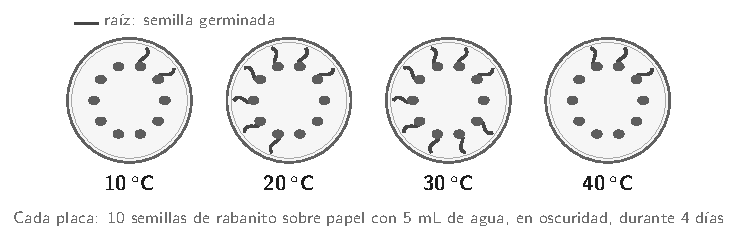
\includegraphics[max width=0.92\linewidth,max height=8.5cm]{bio/hab_germinacion}
\end{center}
  

Un buen procedimiento sigue cinco pasos:

 

\textbf{Paso 1.} Lee el objetivo y nombra la variable independiente (la que vas a cambiar) y la dependiente (la que vas a medir).

 

\textbf{Paso 2.} Elige varios valores de la independiente, bien separados: 10, 20, 30 y 40 °C.

 

\textbf{Paso 3.} Deja \textbf{todo lo demás igual}: misma especie, mismo número de semillas, misma agua, misma luz, mismo tiempo.

 

\textbf{Paso 4.} Decide cómo y con qué medirás la dependiente: contar semillas germinadas al cuarto día.

 

\textbf{Paso 5.} Repite cada condición (varias placas por temperatura) para que el resultado no dependa de una sola placa.

  
\begin{ejemplo}[{Ejemplo resuelto}] En las placas de la figura se ve: 10 °C, 2 de 10 germinadas (20 \%); 20 °C, 7 de 10 (70 \%); 30 °C, 9 de 10 (90 \%); 40 °C, 3 de 10 (30 \%).\par Como en todas las placas hay la misma especie, el mismo número de semillas, la misma agua y la misma oscuridad, la diferencia se puede atribuir a la temperatura.\end{ejemplo}
 
\begin{clave}[{Recuerda}] Si dos grupos difieren en dos variables a la vez (por ejemplo, temperatura y cantidad de agua), no se puede saber cuál de las dos causó la diferencia. Por eso cada ensayo cambia solo la variable independiente.\end{clave}
\subsection{Lo clave del tema}
\begin{center}\small
\begin{tabularx}{\linewidth}{@{}>{\raggedright\arraybackslash\hsize=0.77\hsize}X>{\raggedright\arraybackslash\hsize=1.23\hsize}X@{}}
\toprule
\textbf{Concepto} & \textbf{Lo que tienes que reconocer} \\
\midrule
Pregunta de investigación & Se responde midiendo; calza con lo que se varió y lo que se midió. \\
Hipótesis & Respuesta tentativa que relaciona la variable independiente con la dependiente. \\
Predicción & Resultado concreto esperado: «si\dots{}, entonces\dots{}». \\
Variable independiente & La que se cambia a propósito. \\
Variable dependiente & La que se mide. \\
Variables controladas & Las que se mantienen iguales. \\
Grupo control & Grupo igual a los demás, pero sin el factor estudiado. \\
Teoría / ley / modelo & Por qué pasa / qué pasa / representación simplificada. \\
\bottomrule
\end{tabularx}
\end{center}
 
\begin{clave}[{Recuerda}] · Variable independiente: la que se decide antes; dependiente: la que se mide.\par · La hipótesis habla de la variable que cambia en el experimento.\par · Para estudiar una variable, compara grupos que solo difieren en esa variable.\par · «Germinaron 9 de 10 semillas» es un resultado; la conclusión lo interpreta y responde la pregunta.\par · El objetivo se escribe con un verbo en infinitivo: determinar, evaluar, comparar.\end{clave}
 
\begin{clave}[{Método PAES}] 1. Subraya qué se cambió, qué se midió y qué se dejó igual. 2. Con eso, nombra las tres variables. 3. Si preguntan por la hipótesis o la pregunta, elige la que relaciona exactamente esas dos variables. 4. Si preguntan por un componente, busca las pistas («si\dots{} entonces», «determinar», «se obtuvo», «se sembró»). 5. Descarta las alternativas que hablan de variables que no cambiaron o que no se midieron.\end{clave}
\begin{elejemplo}{Estilo PAES}
Un grupo de estudiantes quiere averiguar qué factores influyen en el crecimiento de plantas de poroto. Para ello prepara cuatro ensayos con plantas de la misma edad y en el mismo tipo de suelo, como se muestra en la figura. Después de tres semanas medirá la altura de las plantas.

¿Cuál de las siguientes comparaciones permite estudiar el efecto de un solo factor?
\begin{center}
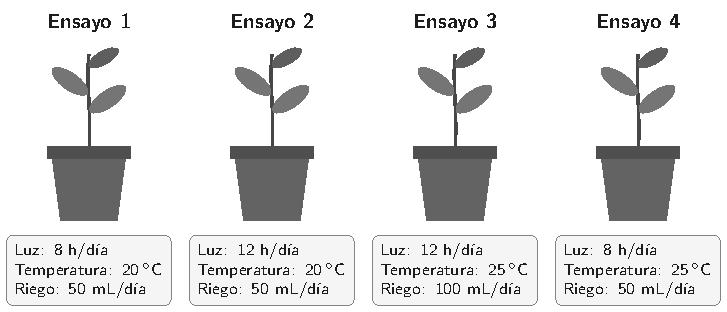
\includegraphics[max width=0.92\linewidth,max height=8.5cm]{bio/hab_macetas}
\end{center}
\altslargas{Comparar los ensayos 1 y 3 permite analizar el efecto del riego.}{Comparar los ensayos 2 y 4 permite analizar el efecto de la temperatura.}{Comparar los ensayos 1 y 4 permite analizar el efecto de la temperatura.}{Comparar los ensayos 3 y 4 permite analizar el efecto de las horas de luz.}
\solucion{\textbf{Paso 1. ¿Qué nos piden?} Un par de ensayos que sirva para estudiar el efecto de \textbf{un} factor. Dos ensayos sirven para estudiar una variable solo si se diferencian \textbf{únicamente} en esa variable. Así, si la altura cambia, sabemos qué lo causó.

\textbf{Paso 2. Ensayos 1 y 3.} Luz: 8 y 12 h (cambia). Temperatura: 20 y 25 °C (cambia). Riego: 50 y 100 mL (cambia). Cambian los tres factores: este par no sirve.

\textbf{Paso 3. Ensayos 2 y 4.} Luz: 12 y 8 h (cambia). Temperatura: 20 y 25 °C (cambia). Riego: 50 y 50 mL (igual). Cambian dos factores: no sirve.

\textbf{Paso 4. Ensayos 1 y 4.} Luz: 8 y 8 h (igual). Temperatura: 20 y 25 °C (cambia). Riego: 50 y 50 mL (igual). Solo cambia la temperatura: este par sirve para estudiar la \textbf{temperatura}.

\textbf{Paso 5. Ensayos 3 y 4.} Luz: 12 y 8 h (cambia). Temperatura: 25 y 25 °C (igual). Riego: 100 y 50 mL (cambia). Cambian dos factores: no sirve.

\textbf{Respuesta:} comparar los ensayos 1 y 4 permite analizar el efecto de la temperatura.

\textbf{Comprobación:} en los ensayos 1 y 4 la temperatura es la variable independiente, y la luz (8 h) y el riego (50 mL/día) son variables controladas. También los ensayos 1 y 2 forman un buen par, pero para estudiar la luz, y esa comparación no está entre las alternativas.

\textbf{¿Por qué no las otras?} «1 y 3 para el riego» elige un par en que cambian los tres factores. «2 y 4 para la temperatura» y «3 y 4 para la luz» eligen pares en que cambian dos factores a la vez; cualquier diferencia en la altura podría deberse a cualquiera de los dos.

\textbf{\color{cienciaD}Para recordar.} Para estudiar una variable, compara solo ensayos que se diferencian únicamente en esa variable.}{C}
\end{elejemplo}
\motivacion{Hipótesis, variables y grupo control: ya diseñas experimentos con orden. La biología también es método.}

%% =====================================================================
%% bio_hab_evidencia
\section[Procesar y analizar evidencia]{Procesar y analizar evidencia}
\modcomun\ \ {\color{gris}\itshape Leer tablas y gráficos de líneas, barras, circulares y de dispersión con datos biológicos, reconocer relaciones directas, inversas y proporcionales, tendencias, máximos y óptimos (como la actividad enzimática según el pH o la temperatura), hacer predicciones e inferencias y calcular promedios y variaciones.\par}
\subsection{Leer una tabla de datos}
Antes de mirar las alternativas, lee la tabla en cuatro pasos:

 

\textbf{Paso 1. Encabezados y unidades.} ¿Qué mide cada columna? ¿En qué unidad?

 

\textbf{Paso 2. ¿Qué cambia y qué se mide?} Identifica la variable independiente y la dependiente.

 

\textbf{Paso 3. Recorre en orden.} Sigue la columna que crece y mira qué hace la otra: ¿sube, baja o queda igual?

 

\textbf{Paso 4. Revisa todas las filas.} Una tendencia vale solo si se cumple en todas.

 
\begin{center}\small
\begin{tabularx}{\linewidth}{@{}>{\raggedright\arraybackslash\hsize=0.85\hsize}X>{\raggedright\arraybackslash\hsize=0.78\hsize}X>{\raggedright\arraybackslash\hsize=1.36\hsize}X@{}}
\toprule
\textbf{Temperatura del agua (°C)} & \textbf{Oxígeno disuelto (mg/L)} & \textbf{Movimientos del opérculo de un pez (por min)} \\
\midrule
5 & 12,8 & 40 \\
10 & 11,3 & 55 \\
15 & 10,1 & 70 \\
20 & 9,1 & 90 \\
\bottomrule
\end{tabularx}
\end{center}
  
\begin{ejemplo}[{Ejemplo resuelto}] En la tabla, la temperatura crece de arriba hacia abajo: 5 \ensuremath{\rightarrow} 10 \ensuremath{\rightarrow} 15 \ensuremath{\rightarrow} 20 °C. Mientras tanto, el oxígeno disuelto baja (12,8 \ensuremath{\rightarrow} 9,1 mg/L) y los movimientos del opérculo, con los que el pez hace pasar agua por sus branquias, suben (40 \ensuremath{\rightarrow} 90 por minuto).\par Relaciones correctas:\par · «El oxígeno disuelto \textbf{disminuye} al aumentar la temperatura» (relación inversa).\par · «Los movimientos del opérculo \textbf{aumentan} al disminuir el oxígeno disuelto» (también inversa, leída al revés).\par Una inferencia razonable: con menos oxígeno en el agua, el pez mueve más agua por sus branquias.\end{ejemplo}
 
\begin{clave}[{Recuerda}] Cuando una alternativa recorre la tabla al revés («al disminuir\dots{}»), recórrela tú también al revés antes de responder. En una relación inversa, si una variable baja, la otra sube.\end{clave}
\subsection{Leer un gráfico: máximos y óptimos}
\begin{center}
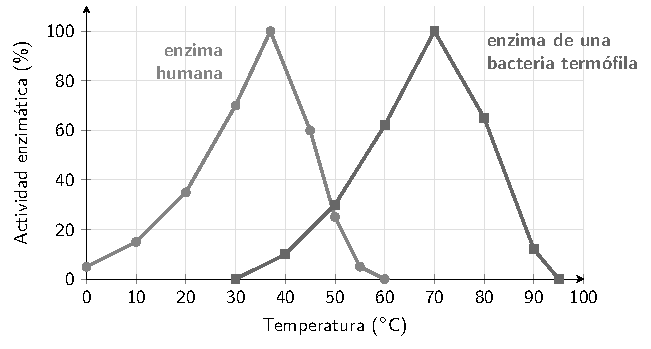
\includegraphics[max width=0.92\linewidth,max height=8.5cm]{bio/hab_enzima_temp}
\end{center}
 

\textbf{Paso 1. Ejes.} Eje horizontal: temperatura (°C), la variable independiente. Eje vertical: actividad enzimática (\%), la variable dependiente.

 

\textbf{Paso 2. Escala.} Cada línea vertical vale 10 °C; cada horizontal, 20 \%.

 

\textbf{Paso 3. Lee puntos.} La enzima humana tiene 35 \% de actividad a 20 °C, 100 \% a 37 °C y 25 \% a 50 °C.

 

\textbf{Paso 4. Busca el máximo.} La temperatura en que la actividad es máxima es la \textbf{temperatura óptima}: 37 °C para la enzima humana y 70 °C para la de la bacteria termófila, que vive en aguas termales.

  
\begin{clave}[{La forma de la curva cuenta la historia}] Bajo el óptimo, la actividad sube con la temperatura, porque las moléculas se mueven más rápido y se encuentran más. Sobre el óptimo, la actividad cae bruscamente: la enzima se \textbf{desnaturaliza}, es decir, pierde su forma y deja de funcionar.\end{clave}
 
\begin{ejemplo}[{Ejemplo resuelto}] ¿A qué temperaturas la enzima humana tiene más de la mitad de su actividad máxima?\par \textbf{Paso 1.} La mitad de 100 \% es 50 \%.\par \textbf{Paso 2.} La curva supera el 50 \% entre unos 25 °C y unos 47 °C.\par \textbf{Paso 3.} En ese rango la actividad es mayor que 50 \%.\end{ejemplo}
 
\begin{clave}[{Recuerda}] Para comparar dos curvas, léelas en el mismo valor del eje horizontal. A 60 °C la enzima bacteriana tiene 62 \% de actividad y la humana, 0 \%.\end{clave}
\subsection{Tipos de gráfico y cuándo usarlos}
\begin{center}
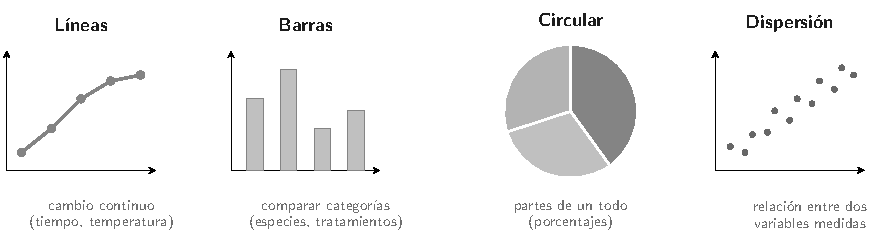
\includegraphics[max width=0.92\linewidth,max height=8.5cm]{bio/hab_graficos}
\end{center}
  
\begin{center}\small
\begin{tabularx}{\linewidth}{@{}>{\raggedright\arraybackslash\hsize=0.42\hsize}X>{\raggedright\arraybackslash\hsize=1.29\hsize}X>{\raggedright\arraybackslash\hsize=1.29\hsize}X@{}}
\toprule
\textbf{Gráfico} & \textbf{Sirve para\dots{}} & \textbf{Ejemplo en biología} \\
\midrule
\textbf{Líneas} & Mostrar cómo cambia una variable a lo largo de otra continua (tiempo, temperatura, pH). & Frecuencia cardíaca durante el ejercicio; crecimiento de una población bacteriana. \\
\textbf{Barras} & Comparar valores entre categorías separadas. & Porcentaje de germinación de cuatro especies. \\
\textbf{Circular} & Mostrar cómo se reparte un total (100 \%) entre sus partes. & Porcentaje de cada tipo de glóbulo blanco en la sangre. \\
\textbf{Dispersión} & Ver si dos variables medidas en muchos individuos se relacionan. & Masa corporal y frecuencia cardíaca de distintos mamíferos. \\
\bottomrule
\end{tabularx}
\end{center}
  
\begin{clave}[{Dónde va cada variable}] En los gráficos de líneas y de dispersión, la variable independiente va en el eje horizontal y la dependiente en el vertical.\end{clave}
 
\begin{ejemplo}[{Ejemplo resuelto}] Un estudiante cuenta los individuos de cinco especies de aves en un humedal. ¿Qué gráfico usa para compararlas?\par Las especies son categorías separadas, sin un orden numérico entre ellas: un \textbf{gráfico de barras}, con una barra por especie.\end{ejemplo}
\subsection{Relaciones entre variables}
\begin{center}
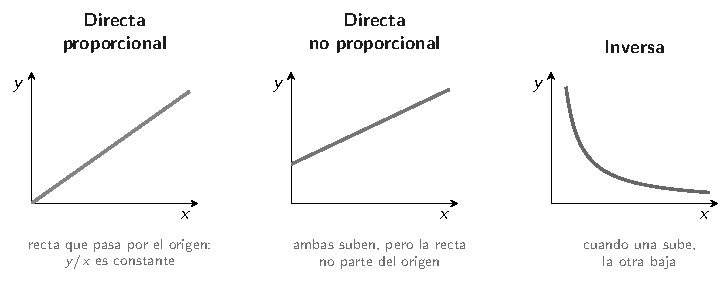
\includegraphics[max width=0.92\linewidth,max height=8.5cm]{bio/hab_relaciones}
\end{center}
  
\begin{center}\small
\begin{tabularx}{\linewidth}{@{}>{\raggedright\arraybackslash\hsize=0.71\hsize}X>{\raggedright\arraybackslash\hsize=1.14\hsize}X>{\raggedright\arraybackslash\hsize=1.14\hsize}X@{}}
\toprule
\textbf{Relación} & \textbf{Qué pasa} & \textbf{Cómo comprobarla} \\
\midrule
Directa & Si una aumenta, la otra también. & Ambas columnas suben juntas. \\
Directamente proporcional & Si una se duplica, la otra se duplica. & El cociente $y/x$ es constante; el gráfico es una recta que pasa por el origen. \\
Inversa & Si una aumenta, la otra disminuye. & Una columna sube y la otra baja. \\
Inversamente proporcional & Si una se duplica, la otra se reduce a la mitad. & El producto $x\cdot y$ es constante. \\
\bottomrule
\end{tabularx}
\end{center}
  
\begin{ejemplo}[{Ejemplo resuelto}] Distintas cantidades de una enzima digieren un trozo igual de gelatina, a la misma temperatura:
\begin{center}\small
\begin{tabular}{@{}lll@{}}
\toprule
\textbf{Enzima (u.a.)} & \textbf{Tiempo (min)} & \textbf{Enzima × tiempo} \\
\midrule
1 & 60 & 60 \\
2 & 30 & 60 \\
3 & 20 & 60 \\
\bottomrule
\end{tabular}
\end{center}
 El producto es siempre 60: el tiempo de digestión es \textbf{inversamente proporcional} a la cantidad de enzima.\end{ejemplo}
 
\begin{clave}[{Recuerda}] Una relación es proporcional solo si el cociente (directa) o el producto (inversa) es constante. La altura de una planta sube con los días, pero si la semilla ya medía 2 cm el primer día, la recta no pasa por el origen: es directa, no proporcional.\end{clave}
\subsection{Tendencias: interpolar y predecir}
Una \textbf{tendencia} es el patrón que siguen los datos. Con ella se puede estimar un valor que no se midió.

 
\begin{itemize}
  \item \textbf{Interpolar}: estimar un valor \textbf{dentro} del rango medido. Es bastante seguro.
  \item \textbf{Extrapolar}: estimar \textbf{fuera} del rango medido. Es arriesgado y solo vale para valores cercanos.
\end{itemize}
 
\begin{center}\small
\begin{tabular}{@{}ll@{}}
\toprule
\textbf{pH del suelo} & \textbf{Crecimiento de una planta de maíz (cm/semana)} \\
\midrule
4 & 2 \\
5 & 5 \\
6 & 8 \\
7 & 7 \\
8 & 3 \\
\bottomrule
\end{tabular}
\end{center}
 

El crecimiento sube hasta pH 6 y luego baja: hay un \textbf{óptimo} cerca de pH 6. A pH 6,5 se espera un valor entre 7 y 8 cm por semana (interpolación).

  
\begin{ejemplo}[{Ejemplo resuelto: predecir con la tendencia}] Una lagartija, cuya temperatura corporal depende del ambiente, consume 0,10 mL de O\textsubscript{2} por gramo y por hora a 10 °C; 0,20 a 20 °C, y 0,40 a 30 °C.\par \textbf{Paso 1.} Cada 10 °C, el consumo se duplica.\par \textbf{Paso 2.} A 25 °C, el consumo debe estar entre 0,20 y 0,40: unos 0,3 mL de O\textsubscript{2} por gramo y por hora.\end{ejemplo}
 
\begin{clave}[{Recuerda}] Una predicción se apoya en la tendencia medida y se limita al rango estudiado o a valores cercanos. Si el maíz se midió entre pH 4 y 8, los datos no dicen qué pasa a pH 2.\end{clave}
\subsection{Cálculos simples: promedio, variación y porcentaje}
Muchas preguntas de evidencia piden un cálculo corto antes de comparar. Sin calculadora, ordena los pasos:

 
\begin{center}\small
\begin{tabularx}{\linewidth}{@{}>{\raggedright\arraybackslash\hsize=0.67\hsize}X>{\raggedright\arraybackslash\hsize=1.33\hsize}X@{}}
\toprule
\textbf{Cálculo} & \textbf{Cómo se hace} \\
\midrule
Promedio & Suma de los valores dividida por cuántos son. \\
Variación & Valor final \ensuremath{-} valor inicial. \\
Variación porcentual & $\dfrac{\text{final} - \text{inicial}}{\text{inicial}}\cdot 100$ \\
Tasa o rapidez & Variación dividida por el tiempo. \\
Eficiencia & Lo obtenido dividido por lo usado. \\
\bottomrule
\end{tabularx}
\end{center}
  
\begin{ejemplo}[{Ejemplo resuelto: promedio de repeticiones}] Tres plantas regadas con un fertilizante crecieron 12, 14 y 13 cm. Promedio: $\dfrac{12 + 14 + 13}{3} = \dfrac{39}{3} = 13$ cm. Un valor aislado alto, como 19 cm en una sola planta, no basta para decir que un tratamiento es mejor: se comparan los promedios.\end{ejemplo}
 
\begin{ejemplo}[{Ejemplo resuelto: variación porcentual}] Una población de 200 coipos pasa a 250 en un año. Variación: $250 - 200 = 50$. Variación porcentual: $\dfrac{50}{200}\cdot 100 = 25\%$. Se divide por el valor \textbf{inicial}.\end{ejemplo}
 
\begin{clave}[{Recuerda}] «Más eficiente», «mayor rendimiento» y «mayor aumento porcentual» piden un cociente, no el número más grande de la tabla.\end{clave}
\subsection{Lo clave del tema}
\begin{center}\small
\begin{tabularx}{\linewidth}{@{}>{\raggedright\arraybackslash\hsize=1.00\hsize}X>{\raggedright\arraybackslash\hsize=1.00\hsize}X@{}}
\toprule
\textbf{Si te piden\dots{}} & \textbf{Haz esto} \\
\midrule
Una relación o tendencia & Recorre la variable que crece y mira qué hace la otra; revisa todas las filas. \\
Saber si es proporcional & Directa: cociente constante, recta por el origen. Inversa: producto constante. \\
Leer un gráfico & Ejes, unidades y escala antes de leer un punto. \\
Un óptimo & Busca el valor del eje horizontal donde la curva es más alta. \\
Una predicción & Sigue la tendencia, sin extrapolar lejos del rango medido. \\
Una conclusión o inferencia & Que salga de los datos, hable solo de lo medido y no agregue nada. \\
Un promedio, una variación o una eficiencia & Calcula para cada grupo y después compara. \\
\bottomrule
\end{tabularx}
\end{center}
 
\begin{clave}[{Recuerda}] · En una relación inversa, cuando una variable disminuye, la otra aumenta.\par · Cada enzima tiene un óptimo de temperatura y de pH; lejos del óptimo, su actividad baja.\par · Que dos variables cambien juntas no prueba que una cause la otra.\par · La conclusión se limita a lo estudiado: «en el rango estudiado, la germinación fue máxima a 30 °C».\par · La variación porcentual se calcula sobre el valor inicial.\end{clave}
 
\begin{clave}[{Método PAES}] 1. Lee encabezados, ejes y unidades. 2. Identifica qué cambió y qué se midió. 3. Describe en tu cabeza la tendencia antes de leer las alternativas. 4. Si hay números, calcula el promedio, la diferencia, el cociente o el producto que corresponda. 5. Descarta lo que no sale de los datos, lo que generaliza y lo que habla de variables que no se midieron.\end{clave}
\begin{elejemplo}{PAES Regular 2026, adaptada}
En un laboratorio se mide la actividad de dos enzimas digestivas humanas a distintos valores de pH, manteniendo la temperatura en 37 °C. La pepsina actúa en el estómago y la amilasa salival, en la boca. Los resultados se muestran en el gráfico:

¿Cuál de las siguientes afirmaciones describe correctamente los resultados?
\begin{center}
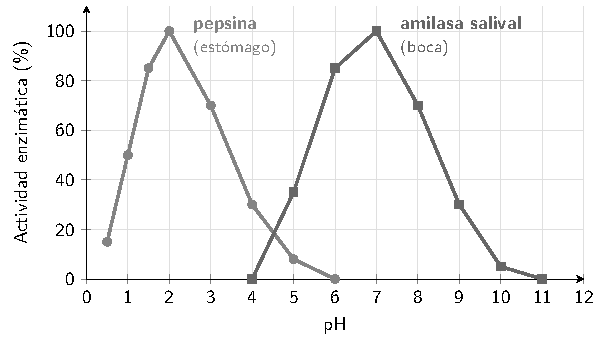
\includegraphics[max width=0.92\linewidth,max height=8.5cm]{bio/hab_enzima_ph}
\end{center}
\altslargas{Ambas enzimas alcanzan su máxima actividad al mismo pH.}{A pH 7, la pepsina alcanza su máxima actividad.}{Cada enzima tiene un pH óptimo, y su actividad disminuye al alejarse de él hacia valores más ácidos o más básicos.}{La actividad de la amilasa salival aumenta siempre al aumentar el pH.}
\solucion{\textbf{Paso 1. ¿Qué nos piden?} La afirmación que describe bien el gráfico. Primero lo leemos y después revisamos cada alternativa.

\textbf{Paso 2. Lee los ejes.} Eje horizontal: pH, de 0 a 12. Eje vertical: actividad enzimática en \%. Cada línea horizontal vale 20 \%.

\textbf{Paso 3. Lee la pepsina.} Sube desde pH 0,5 hasta su máximo (100 \%) a pH 2 y luego baja hasta 0 \% a pH 6.

\textbf{Paso 4. Lee la amilasa.} Es 0 \% a pH 4, sube hasta 100 \% a pH 7 y baja hasta 0 \% a pH 11.

\textbf{Paso 5. Describe la tendencia.} Las dos curvas tienen un máximo, el \textbf{pH óptimo}: 2 para la pepsina y 7 para la amilasa. A ambos lados del óptimo, la actividad disminuye.

\textbf{Respuesta:} cada enzima tiene un pH óptimo, y su actividad disminuye al alejarse de él hacia valores más ácidos o más básicos.

\textbf{Comprobación:} los óptimos calzan con el lugar donde actúa cada enzima. El estómago es muy ácido (pH cercano a 2) y la boca es casi neutra (pH cercano a 7).

\textbf{¿Por qué no las otras?} «Al mismo pH» es falsa: los máximos están en pH 2 y en pH 7. «A pH 7 la pepsina alcanza su máximo» es falsa: a pH 7 la pepsina tiene 0 \% de actividad. «La amilasa aumenta siempre» solo se cumple hasta pH 7; desde ahí baja hasta 0 \% a pH 11.

\textbf{\color{cienciaD}Para recordar.} Una curva con un máximo indica un óptimo: la actividad baja al alejarse de él hacia ambos lados.}{C}
\end{elejemplo}
\motivacion{Interpretar resultados es separar lo que dicen los datos de lo que uno cree. Ya tienes ese ojo crítico.}

%% =====================================================================
%% bio_hab_evaluar
\section[Evaluar y comunicar]{Evaluar y comunicar}
\modcomun\ \ {\color{gris}\itshape Juzgar si una conclusión está respaldada por los datos, reconocer el alcance y los límites de un estudio sin generalizar, evaluar la validez y la confiabilidad del diseño (comparaciones justas, grupo control, tamaño de muestra, repeticiones), distinguir resultado de conclusión y elegir el recurso adecuado para comunicar.\par}
\subsection{Validez y confiabilidad}
\textbf{Validez:} la investigación mide de verdad lo que dice medir y su diseño permite sacar la conclusión. Falla cuando no se controlaron variables, cuando falta un grupo control o cuando se mide una variable distinta de la que se quiere estudiar.

 

\textbf{Confiabilidad:} al repetir las mediciones se obtienen resultados parecidos. Mejora con más repeticiones, con muestras más grandes y con instrumentos más precisos.

 

\textbf{Precisión y exactitud.} Mediciones \textbf{precisas} son cercanas entre sí. Mediciones \textbf{exactas} son cercanas al valor real. Un termómetro mal calibrado que siempre marca 2 °C de más es preciso, pero no exacto.

 
\begin{center}\small
\begin{tabularx}{\linewidth}{@{}>{\raggedright\arraybackslash\hsize=0.67\hsize}X>{\raggedright\arraybackslash\hsize=1.33\hsize}X@{}}
\toprule
\textbf{Factor} & \textbf{Por qué importa} \\
\midrule
Tamaño de la muestra & Un solo individuo puede ser excepcional; con muchos, las diferencias individuales se compensan. \\
Repeticiones & Permiten ver si el resultado se mantiene y calcular promedios. \\
Instrumento adecuado & Un instrumento poco preciso agrega variación que no viene del fenómeno. \\
\bottomrule
\end{tabularx}
\end{center}
  
\begin{ejemplo}[{Ejemplo resuelto}] Un equipo prueba un fármaco para mejorar la calidad de los espermatozoides de una especie en peligro de extinción. Lo aplica a \textbf{un solo} macho y su calidad espermática mejora. Una comisión rechaza el estudio por baja confiabilidad.\par \textbf{¿Qué lo mejora?} Probar el fármaco en un número mayor de machos de la \textbf{misma especie}, en las mismas condiciones, y compararlos con machos sin tratamiento. Con un solo individuo, la mejora podría deberse al azar o a algo propio de ese animal.\end{ejemplo}
 
\begin{clave}[{Recuerda}] Aumentar la muestra significa más individuos del mismo tipo que se estudia. Probar en otras especies o en individuos sanos responde otra pregunta.\end{clave}
\subsection{¿La conclusión está respaldada por los datos?}
Para evaluar una conclusión, revisa esta lista:

 

\textbf{1. ¿Responde la pregunta u objetivo?}

 

\textbf{2. ¿Habla solo de las variables medidas y del rango estudiado?}

 

\textbf{3. ¿El diseño permite comparar?} Para afirmar que un tratamiento produce un efecto, hace falta un grupo sin tratamiento.

 

\textbf{4. ¿Se controlaron las demás variables?} Si cambiaron dos cosas a la vez, no se puede atribuir el efecto a una sola.

 

\textbf{5. ¿Hay suficientes individuos y repeticiones?} Un solo ensayo da una conclusión débil.

  
\begin{ejemplo}[{Ejemplo resuelto}] Una empresa afirma: «nuestra crema elimina el hongo de los pies en 4 semanas». La aplicó a 50 personas con el hongo y, después de 4 semanas, 40 estaban sanas.\par \textbf{Evaluación:} el resultado no basta para atribuir la mejoría a la crema, porque \textbf{falta un grupo control}: personas con el hongo tratadas con una crema igual, pero sin el principio activo. Sin ese grupo, no se sabe cuántas se habrían recuperado de todos modos.\end{ejemplo}
 
\begin{clave}[{Recuerda}] Un diseño puede ser incapaz de responder la pregunta aunque cada medición esté bien hecha. Evaluar una conclusión es revisar tanto los datos como el diseño que los produjo.\end{clave}
\subsection{Alcance y límites: no generalizar}
Una conclusión vale para las condiciones en que se obtuvo. Antes de aceptar una alternativa, revisa sus límites:

 
\begin{center}\small
\begin{tabularx}{\linewidth}{@{}>{\raggedright\arraybackslash\hsize=0.90\hsize}X>{\raggedright\arraybackslash\hsize=1.10\hsize}X@{}}
\toprule
\textbf{Si el estudio se hizo\dots{}} & \textbf{la conclusión vale para\dots{}} \\
\midrule
con una especie & esa especie; otras especies requieren otros estudios. \\
entre 10 y 30 °C & ese rango de temperatura. \\
con células en cultivo (in vitro) & esas células; en un organismo completo hay que comprobarlo. \\
en el laboratorio & condiciones de laboratorio; en terreno pueden influir otros factores. \\
con 12 lagos de una región & lagos parecidos a esos. \\
\bottomrule
\end{tabularx}
\end{center}
 

Las alternativas correctas suelen usar expresiones prudentes: «en las condiciones del estudio», «en el rango estudiado», «podría».

  
\begin{clave}[{Correlación y causa}] En un estudio de \textbf{observación} el investigador solo registra lo que ya ocurre (por ejemplo, la dieta y la presión arterial de 500 personas). Si dos variables cambian juntas, hay una \textbf{asociación}, pero puede deberse a un tercer factor. Para mostrar que una variable \textbf{causa} otra, se necesita un experimento que cambie esa variable y controle las demás.\end{clave}
 
\begin{ejemplo}[{Ejemplo resuelto}] Un compuesto elimina el 90 \% de las células de cáncer de pulmón humano en cultivo.\par \textbf{Alcance razonable:} «el compuesto podría ser útil contra el cáncer de pulmón; falta probar su efecto y su seguridad en organismos completos».\par Afirmar que cura a las personas, que sirve para todo cáncer o que no daña las células sanas va más allá de lo que se midió.\end{ejemplo}
\subsection{Comparaciones justas y cómo mejorar un diseño}
\begin{center}\small
\begin{tabularx}{\linewidth}{@{}>{\raggedright\arraybackslash\hsize=1.00\hsize}X>{\raggedright\arraybackslash\hsize=1.00\hsize}X@{}}
\toprule
\textbf{Limitación} & \textbf{Mejora} \\
\midrule
Un solo individuo o un solo ensayo & Usar más individuos y repetir. \\
Falta un grupo control & Agregar un grupo igual, pero sin el factor estudiado. \\
Los grupos difieren en más de una variable & Cambiar solo la variable independiente. \\
La variable independiente no alcanza el efecto buscado & Ampliar el rango de valores. \\
Se mide otra variable & Medir la variable que plantea el objetivo. \\
Instrumento poco preciso & Usar uno más preciso o repetir la medición. \\
\bottomrule
\end{tabularx}
\end{center}
  
\begin{ejemplo}[{Ejemplo resuelto}] Para comparar dos fertilizantes, un estudiante pone las plantas del fertilizante X junto a una ventana soleada y las del fertilizante Y en un pasillo con sombra. Las del X crecen más.\par \textbf{Paso 1.} ¿Qué difiere entre los grupos? El fertilizante \textbf{y} la luz.\par \textbf{Paso 2.} Como la luz influye en la fotosíntesis, la diferencia podría deberse a ella.\par \textbf{Mejora:} poner los dos grupos en el mismo lugar, con la misma luz, el mismo riego y plantas de la misma especie y edad.\end{ejemplo}
 
\begin{clave}[{Recuerda}] La mejora correcta corrige el defecto que impide responder la pregunta. Si el problema es la luz, medir más seguido o agregar fertilizante no lo resuelve.\end{clave}
\subsection{Resultado, inferencia y conclusión}
Las tres se parecen, pero cumplen papeles distintos. Míralas en un mismo estudio: 40 adultos con presión alta se dividen en dos grupos de 20; uno reduce la sal de su dieta y el otro mantiene su dieta habitual durante 8 semanas.

 
\begin{center}\small
\begin{tabularx}{\linewidth}{@{}>{\raggedright\arraybackslash\hsize=0.57\hsize}X>{\raggedright\arraybackslash\hsize=1.43\hsize}X@{}}
\toprule
\textbf{Componente} & \textbf{En el estudio} \\
\midrule
\textbf{Procedimiento} & «Se midió la presión arterial de cada persona antes y después de 8 semanas». \\
\textbf{Resultado} & «En el grupo que redujo la sal, la presión bajó en promedio 12 mmHg; en el otro grupo, 1 mmHg». \\
\textbf{Conclusión} & «En las personas estudiadas, reducir la sal de la dieta disminuyó la presión arterial». \\
\textbf{Inferencia} & «Reducir la sal podría disminuir el riesgo de enfermedades del corazón en estas personas». \\
\bottomrule
\end{tabularx}
\end{center}
  
\begin{clave}[{Cómo distinguirlas}] · El \textbf{resultado} da los datos, con números o con lo observado.\par · La \textbf{conclusión} interpreta los resultados y responde la pregunta del estudio.\par · La \textbf{inferencia} va un paso más allá de lo medido; por eso suele decir «podría».\end{clave}
 
\begin{clave}[{Replicar y reproducir}] Un procedimiento es \textbf{replicable} si está descrito con tanto detalle (especie, cantidades, temperatura, tiempo) que otra persona puede repetirlo. Un resultado es \textbf{reproducible} si al repetirlo se obtiene algo equivalente. Por eso un informe detalla el procedimiento completo.\end{clave}
\subsection{Comunicar resultados}
\begin{center}
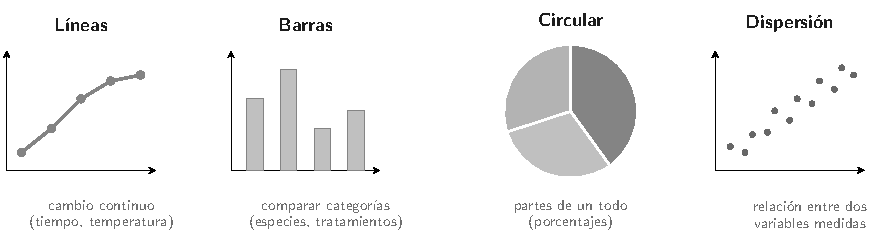
\includegraphics[max width=0.92\linewidth,max height=8.5cm]{bio/hab_graficos}
\end{center}
  
\begin{center}\small
\begin{tabularx}{\linewidth}{@{}>{\raggedright\arraybackslash\hsize=1.31\hsize}X>{\raggedright\arraybackslash\hsize=0.69\hsize}X@{}}
\toprule
\textbf{Objetivo} & \textbf{Recurso} \\
\midrule
Mostrar cómo cambia una variable en el tiempo o con la temperatura & Gráfico de líneas \\
Comparar especies, tratamientos o grupos & Gráfico de barras \\
Mostrar cómo se reparte un total (100 \%) & Gráfico circular \\
Ver si dos variables medidas se relacionan & Gráfico de dispersión \\
Entregar valores exactos o muchas variables & Tabla \\
Mostrar una estructura o un proceso & Esquema o modelo \\
\bottomrule
\end{tabularx}
\end{center}
  
\begin{ejemplo}[{Ejemplo resuelto}] Un equipo mide, en 30 personas, la masa corporal y la cantidad de sangre que bombea el corazón en un minuto. Quiere mostrar si estas variables se relacionan.\par Son dos variables numéricas medidas en cada persona: un \textbf{gráfico de dispersión}, con un punto por persona.\end{ejemplo}
 
\begin{clave}[{Recuerda}] Un buen gráfico tiene título, ejes con nombre y unidad, y la variable independiente en el eje horizontal. El informe de una investigación incluye objetivo, procedimiento, resultados y conclusión.\end{clave}
\subsection{Lo clave del tema}
\begin{center}\small
\begin{tabularx}{\linewidth}{@{}>{\raggedright\arraybackslash\hsize=0.75\hsize}X>{\raggedright\arraybackslash\hsize=1.25\hsize}X@{}}
\toprule
\textbf{Si te piden\dots{}} & \textbf{Revisa esto} \\
\midrule
Evaluar una conclusión & ¿Sale de los datos? ¿Habla solo de lo medido? ¿El diseño permite compararla? \\
El alcance de un estudio & Especie, rango, tipo de muestra y condiciones en que se hizo. \\
Validez & ¿Se midió lo que se quería medir? ¿Hay grupo control? ¿Se controlaron las variables? \\
Confiabilidad & Número de individuos, repeticiones y precisión del instrumento. \\
Mejorar el diseño & La mejora que corrige el defecto que impide responder la pregunta. \\
Resultado o conclusión & Resultado = datos; conclusión = respuesta a la pregunta. \\
Comunicar & El recurso que calza con el objetivo: líneas, barras, circular, dispersión, tabla o esquema. \\
\bottomrule
\end{tabularx}
\end{center}
 
\begin{clave}[{Recuerda}] · Un efecto se atribuye a un tratamiento solo si hay un grupo control comparable.\par · Más individuos de la misma especie y más repeticiones aumentan la confiabilidad.\par · Lo que se mide en células en cultivo o en una especie debe comprobarse antes de aplicarlo a personas o a otras especies.\par · Una asociación entre dos variables no basta para afirmar que una causa la otra.\par · Los datos valen dentro del rango estudiado: fuera de él no se puede afirmar un óptimo ni un valor.\end{clave}
 
\begin{clave}[{Método PAES}] 1. Identifica el objetivo y las variables del estudio. 2. Revisa el diseño: grupo control, variables controladas, número de individuos y repeticiones. 3. Compara la alternativa con los datos y con su rango. 4. Desconfía de «siempre», «todos», «cualquier», «demuestra» y «cura». 5. Si piden comunicar, elige el recurso según lo que se quiere mostrar.\end{clave}
\begin{elejemplo}{PAES Invierno 2026, adaptada}
Unos estudiantes siembran la bacteria \emph{Escherichia coli} en una placa y colocan cuatro discos de papel: tres empapados en los antibióticos A, B y C, y uno (K) empapado solo en agua. Después de 24 horas a 37 °C miden el diámetro de la zona sin bacterias (halo) alrededor de cada disco, como muestra la figura. Con estos datos concluyen: «el antibiótico B es el más eficaz contra todas las bacterias que causan infecciones».

¿Cuál de las siguientes opciones evalúa correctamente esta conclusión?
\begin{center}
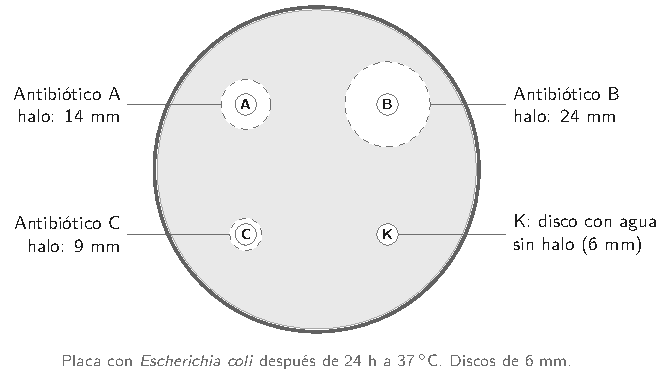
\includegraphics[max width=0.92\linewidth,max height=8.5cm]{bio/hab_antibiotico}
\end{center}
\altslargas{Está respaldada, porque el halo del antibiótico B es el mayor de la placa.}{No está respaldada, porque los datos solo permiten comparar los antibióticos frente a \emph{E. coli}, y se obtuvieron en una sola placa, sin repeticiones.}{No está respaldada, porque el disco K también debió contener un antibiótico.}{Está respaldada, porque el disco K, sin antibiótico, no formó halo.}
\solucion{\textbf{Paso 1. ¿Qué nos piden?} Decidir si la conclusión se sostiene con los datos y con el diseño.

\textbf{Paso 2. ¿Qué muestran los datos?} Halos de 24 mm (B), 14 mm (A), 9 mm (C) y ninguno en K. Contra \emph{E. coli}, en esta placa, el antibiótico B inhibió el crecimiento en la zona más amplia. El disco K muestra que el papel con agua no inhibe a la bacteria.

\textbf{Paso 3. ¿Qué dice la conclusión?} Habla de «todas las bacterias que causan infecciones». Pero se probó \textbf{una sola especie}; otras bacterias pueden responder distinto a cada antibiótico.

\textbf{Paso 4. ¿Y la confiabilidad?} Hay una sola placa y un disco por antibiótico. Para comparar con seguridad se necesitan repeticiones.

\textbf{Respuesta:} no está respaldada, porque los datos solo permiten comparar los antibióticos frente a \emph{E. coli}, y se obtuvieron en una sola placa, sin repeticiones.

\textbf{Una conclusión que sí se sostiene:} «en este ensayo, el antibiótico B produjo el mayor halo de inhibición sobre \emph{E. coli}».

\textbf{¿Por qué no las otras?} «El halo de B es el mayor» es cierto, pero solo para \emph{E. coli}: no justifica hablar de todas las bacterias. «K debió tener antibiótico» se equivoca: K es el grupo control y por eso no debe tenerlo. «K no formó halo» confirma que el control funcionó, pero no resuelve la generalización a otras bacterias.

\textbf{\color{cienciaD}Para recordar.} Una conclusión vale para lo que se probó: la especie, las condiciones y el número de ensayos del estudio.}{B}
\end{elejemplo}
\motivacion{Terminaste Biología y el libro completo: Química, Física y Biología. Los gatitos están muy orgullosos de ti. ¡Ahora a practicar en la página!}

\fi

\end{document}
"
\ifdefined\solocap \input{\solocap} \else
%% Generado por html2tex.py desde temas.json (qui). No editar a mano: corregir la clase en el .js del sitio y regenerar.
\parteciencia{qui}
\chapter{Estructura atómica}
%% =====================================================================
%% qui_mezclas
\section[Sustancias puras y mezclas]{Sustancias puras y mezclas}
\modcomun\ \ {\color{gris}\itshape Cómo se clasifica la materia (elementos, compuestos, mezclas homogéneas y heterogéneas) y cómo se separan las mezclas por filtración, tamizado, decantación y destilación, con sus aplicaciones.\par}
\subsection{Cómo se clasifica la materia}
Todo lo que tiene masa y ocupa espacio es \textbf{materia}. Para ordenarla, la química se hace una primera pregunta: ¿está formada por \textbf{una sola sustancia} o por \textbf{varias}?

 

\textbf{Sustancia pura.} Tiene composición fija y propiedades constantes: siempre funde y hierve a la misma temperatura (a igual presión). Hay dos tipos:

 
\begin{itemize}
  \item \textbf{Elemento:} formado por un solo tipo de átomo. Ejemplos: hierro (Fe), oxígeno (O\textsubscript{2}), helio (He).
  \item \textbf{Compuesto:} dos o más elementos unidos químicamente en una proporción fija. Ejemplos: agua (H\textsubscript{2}O), sal (NaCl), dióxido de carbono (CO\textsubscript{2}).
\end{itemize}
 

\textbf{Mezcla.} Dos o más sustancias juntas, sin reaccionar, en proporción variable. Cada una conserva sus propiedades y se pueden separar por \textbf{métodos físicos}. Hay dos tipos:

 
\begin{itemize}
  \item \textbf{Homogénea:} se ve uniforme, una sola fase. Ejemplos: agua con sal, aire, vinagre, bronce.
  \item \textbf{Heterogénea:} se distinguen dos o más fases. Ejemplos: agua con aceite, arena con agua, granito.
\end{itemize}
  
\begin{clave}[{Cómo leer un diagrama de partículas}] Cada color es un tipo de átomo. Mira cuántos \textbf{tipos de partículas} hay en el recuadro:\par · un solo tipo de partícula \ensuremath{\rightarrow} sustancia pura (si tiene un color, elemento; si tiene dos o más colores unidos, compuesto);\par · dos o más tipos de partículas \ensuremath{\rightarrow} mezcla.\end{clave}
  
\begin{center}
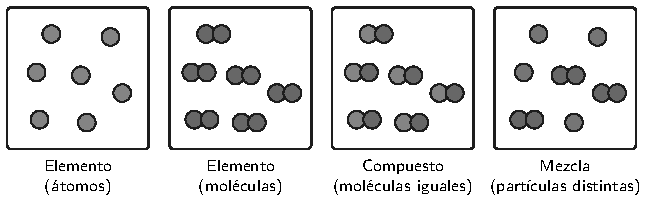
\includegraphics[max width=0.92\linewidth,max height=8.5cm]{qui/atomo_particulas}
\end{center}
\subsection{Elementos y compuestos}
Un \textbf{elemento} no se puede descomponer en sustancias más simples, ni siquiera con una reacción química. Hay cerca de 118, todos en la tabla periódica. Algunos están como átomos sueltos (He, Ne, Fe) y otros como moléculas de átomos iguales (O\textsubscript{2}, N\textsubscript{2}, Cl\textsubscript{2}, O\textsubscript{3}).

 

Un \textbf{compuesto} sí se puede descomponer, pero solo con una \textbf{reacción química}. Por ejemplo, al pasar corriente eléctrica por agua (electrólisis) se obtienen dos gases: hidrógeno y oxígeno.

 

Dos ideas importantes de los compuestos:

 
\begin{itemize}
  \item \textbf{Proporción fija:} el agua siempre tiene 1 g de hidrógeno por cada 8 g de oxígeno, venga de un río o de un glaciar.
  \item \textbf{Propiedades nuevas:} el sodio es un metal que reacciona violentamente con el agua y el cloro es un gas verde y tóxico; juntos forman la sal de mesa, NaCl, que comemos todos los días.
\end{itemize}
  
\begin{ejemplo}[{Ejemplo resuelto}] Clasifica: oro, aire, agua destilada, bronce, CO\textsubscript{2} y ozono (O\textsubscript{3}).\par · Oro (Au): un tipo de átomo \ensuremath{\rightarrow} \textbf{elemento}.\par · Ozono (O\textsubscript{3}): tres átomos, pero todos de oxígeno \ensuremath{\rightarrow} \textbf{elemento}.\par · Agua destilada (H\textsubscript{2}O) y CO\textsubscript{2}: dos elementos unidos \ensuremath{\rightarrow} \textbf{compuestos}.\par · Aire (N\textsubscript{2}, O\textsubscript{2}, Ar, CO\textsubscript{2}\dots{}) y bronce (cobre con estaño): varias sustancias, uniformes \ensuremath{\rightarrow} \textbf{mezclas homogéneas}.\end{ejemplo}
 
\begin{ojo}[{Error típico}] «El O\textsubscript{2} es un compuesto porque tiene dos átomos». No: para ser compuesto debe tener átomos de \textbf{elementos distintos}. Y el agua de la llave no es sustancia pura: lleva sales disueltas. La sustancia pura es el agua destilada.\end{ojo}
\subsection{Mezclas homogéneas y heterogéneas}
Una \textbf{fase} es una parte de la mezcla con el mismo aspecto y las mismas propiedades en todos sus puntos.

 
\begin{itemize}
  \item \textbf{Mezcla homogénea} (o solución): una sola fase. No distingues sus componentes ni con lupa: agua con azúcar, aire, vinagre, acero, bronce.
  \item \textbf{Mezcla heterogénea}: dos o más fases. Agua con aceite, arena con agua, granito, ensalada. La leche y la niebla (coloides) también se clasifican como heterogéneas: al microscopio se ven gotitas o partículas separadas.
\end{itemize}
 

\textbf{¿Por qué el agua y el aceite no se mezclan?} Por la regla «\textbf{lo semejante disuelve a lo semejante}»: las sustancias \textbf{polares} (agua, etanol, acetona) se mezclan entre sí y disuelven sales como el NaCl; las \textbf{apolares} (aceite, hexano, bencina) se mezclan entre sí. Un líquido polar con uno apolar forma dos fases: es una mezcla heterogénea.

  
\begin{clave}[{Esquema para clasificar}] 1. ¿Es uniforme en todos sus puntos? \textbf{No} \ensuremath{\rightarrow} mezcla heterogénea.\par 2. Si es uniforme: ¿se separa por procesos físicos (evaporar, destilar)? \textbf{Sí} \ensuremath{\rightarrow} mezcla homogénea.\par 3. Si no se separa por procesos físicos: ¿se descompone por procesos químicos? \textbf{Sí} \ensuremath{\rightarrow} compuesto. \textbf{No} \ensuremath{\rightarrow} elemento.\end{clave}
 
\begin{ejemplo}[{Ejemplo resuelto}] Al agregar sal a dos líquidos, se disuelve en el líquido T y queda en el fondo del líquido M. Entonces T se comporta como polar y M como apolar. Si se mezclan T y M, se formarán \textbf{dos fases}: una mezcla heterogénea.\end{ejemplo}
 
\begin{ojo}[{Ojo}] «Transparente» no significa «sustancia pura». El agua con sal es transparente y es una mezcla homogénea.\end{ojo}
\subsection{Separar mezclas: filtración y tamizado}
Como en una mezcla cada sustancia conserva sus propiedades, se separan aprovechando una \textbf{diferencia en alguna propiedad física}: tamaño de partícula, densidad, temperatura de ebullición o solubilidad.

 

\textbf{Filtración.} Separa un \textbf{sólido que no está disuelto} de un líquido. La mezcla pasa por un papel filtro: el sólido queda arriba (\textbf{residuo}) y el líquido pasa (\textbf{filtrado}). Se basa en el tamaño de las partículas. Ejemplos: colar el café, los filtros de agua, la mascarilla.

 

\textbf{Tamizado.} Separa \textbf{sólidos de distinto tamaño} con una malla o tamiz: los granos chicos pasan y los grandes quedan. Ejemplos: cernir harina, separar piedras de la arena en una construcción, clasificar mineral en la minería.

  
\begin{center}
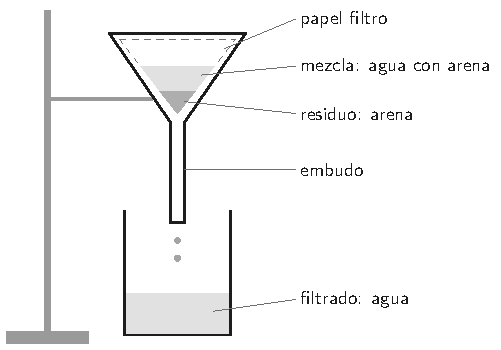
\includegraphics[max width=0.92\linewidth,max height=8.5cm]{qui/atomo_filtracion}
\end{center}
 
\begin{ojo}[{Error típico}] «Filtrando agua de mar obtengo agua sin sal». No: la sal está \textbf{disuelta}, sus partículas son tan pequeñas como las del agua y atraviesan el papel. Lo disuelto no se filtra.\end{ojo}
\subsection{Decantación}
La \textbf{decantación} separa componentes de \textbf{distinta densidad} que no se mezclan.

 

\textbf{Dos líquidos inmiscibles} (agua y aceite): se usa un \textbf{embudo de decantación}. Se deja reposar; el líquido más denso queda abajo. Se abre la llave, sale el líquido de abajo y se cierra justo cuando llega la línea que separa las fases.

 

\textbf{Sólido y líquido} (barro en agua): se deja reposar hasta que el sólido se va al fondo (sedimenta) y se vacía con cuidado el líquido de arriba.

 

\textbf{Aplicación: agua potable.} En las plantas de tratamiento se agregan \textbf{floculantes}, que juntan las partículas pequeñas en grumos (flóculos) más densos que el agua. Los flóculos se van al fondo (\textbf{decantación}) y lo que queda en suspensión se retiene con filtros de arena (\textbf{filtración}).

  
\begin{center}
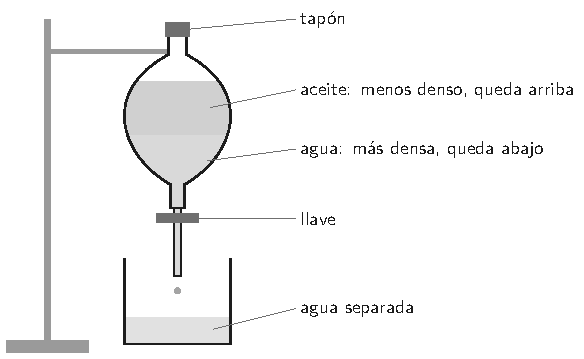
\includegraphics[max width=0.92\linewidth,max height=8.5cm]{qui/atomo_decantacion}
\end{center}
 
\begin{clave}[{Pariente cercano: la centrifugación}] Hace girar la mezcla muy rápido para que lo más denso se vaya al fondo en minutos. Así se separan el plasma y las células de la sangre.\end{clave}
\subsection{Destilación y evaporación}
\textbf{Destilación.} Separa un líquido de lo que tiene disuelto, o dos líquidos \textbf{miscibles} con distinta \textbf{temperatura de ebullición}. Se calienta la mezcla; el componente más volátil (menor temperatura de ebullición) se evapora primero, el vapor se enfría en el \textbf{refrigerante} y se recoge como líquido: el \textbf{destilado}.

 

La \textbf{destilación fraccionada} usa una columna para separar varios líquidos de temperaturas de ebullición cercanas. Así se separa el petróleo en gas, bencina, kerosene y diésel, y así se obtiene el pisco a partir del vino.

 

\textbf{Evaporación.} Si solo interesa el sólido disuelto, se evapora el líquido y el sólido queda. Así se obtiene la sal en las salinas de la costa y el litio en el Salar de Atacama.

  
\begin{clave}[{Mezclas de tres componentes}] Se separan por pasos, cada uno con su propiedad.\par · Arena + sal disuelta en agua: \textbf{filtrar} (queda la arena) y luego \textbf{evaporar} el filtrado (queda la sal).\par · Dos líquidos miscibles + un sólido insoluble: \textbf{filtrar} el sólido y luego \textbf{destilar} los líquidos.\end{clave}
  
\begin{center}
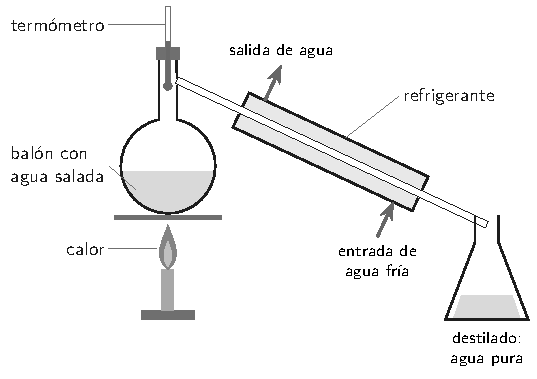
\includegraphics[max width=0.92\linewidth,max height=8.5cm]{qui/atomo_destilacion}
\end{center}
\subsection{Lo clave del tema}
\begin{center}\small
\begin{tabularx}{\linewidth}{@{}>{\raggedright\arraybackslash\hsize=0.51\hsize}X>{\raggedright\arraybackslash\hsize=1.45\hsize}X>{\raggedright\arraybackslash\hsize=0.91\hsize}X>{\raggedright\arraybackslash\hsize=1.13\hsize}X@{}}
\toprule
\textbf{Método} & \textbf{Qué separa} & \textbf{Propiedad que aprovecha} & \textbf{Ejemplo} \\
\midrule
Filtración & sólido no disuelto de un líquido & tamaño de partícula & arena del agua, café \\
Tamizado & sólidos de distinto tamaño & tamaño de partícula & piedras de la arena, harina \\
Decantación & líquidos inmiscibles, o sólido que sedimenta & densidad & agua y aceite, floculantes \\
Destilación & líquidos miscibles, o líquido de su soluto & temperatura de ebullición & petróleo, pisco, agua destilada \\
Evaporación & sólido disuelto de su solvente & volatilidad del solvente & sal de mar, litio \\
\bottomrule
\end{tabularx}
\end{center}
 
\begin{clave}[{Recuerda}] · O\textsubscript{2} es un elemento: todos sus átomos son iguales.\par · Un compuesto tiene partículas iguales formadas por átomos distintos; si hay dos tipos de partículas, es mezcla.\par · El agua con sal es transparente y es una mezcla homogénea.\par · La sal disuelta se separa evaporando o destilando.\par · Dos líquidos miscibles (una sola fase) se separan por destilación.\end{clave}
 
\begin{clave}[{Método PAES}] 1. Cuenta los tipos de partículas o de sustancias: uno \ensuremath{\rightarrow} sustancia pura; varios \ensuremath{\rightarrow} mezcla. 2. Pregunta si es uniforme (homogénea o heterogénea). 3. Para separar, identifica en qué se diferencian los componentes (tamaño, densidad, temperatura de ebullición) y elige el método que usa esa diferencia. 4. Si hay tres componentes, ordena los pasos: primero lo que no está disuelto, al final lo disuelto.\end{clave}
\begin{elejemplo}{PAES Invierno 2027, adaptada}
Un grupo de estudiantes recibe en el laboratorio una muestra de un material desconocido. Para clasificarlo, siguen una secuencia de preguntas y anotan las respuestas en el siguiente esquema:
\begin{center}
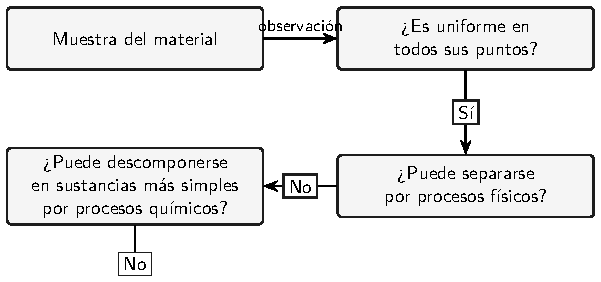
\includegraphics[max width=0.92\linewidth,max height=8.5cm]{qui/atomo_esquema}
\end{center}
\alts{A un elemento.}{A un compuesto.}{A una mezcla homogénea.}{A una mezcla heterogénea.}
\solucion{\textbf{Paso 1. ¿Qué nos piden?} Clasificar el material siguiendo las respuestas del esquema, una por una.

\textbf{Paso 2. ¿Es uniforme? Sí.} Tiene una sola fase. Queda descartada la mezcla heterogénea. Todavía puede ser mezcla homogénea, compuesto o elemento.

\textbf{Paso 3. ¿Se separa por procesos físicos? No.} Una mezcla homogénea, como el agua con sal, sí se separa por procesos físicos (evaporando el agua queda la sal). Como este material no se separa, no es mezcla: es una \textbf{sustancia pura}.

\textbf{Paso 4. ¿Se descompone por procesos químicos? No.} Un compuesto, como el agua, sí se descompone por una reacción química (la electrólisis la separa en hidrógeno y oxígeno). Como este material no se descompone en sustancias más simples, está formado por un solo tipo de átomo.

\textbf{Respuesta:} es un elemento.

\textbf{Comprobación:} un trozo de cobre cumple las tres respuestas: es uniforme, no se separa por filtración, destilación ni evaporación, y ninguna reacción lo convierte en sustancias más simples.

\textbf{¿Por qué no las otras?} «Compuesto» habría tenido «Sí» en la última pregunta: los compuestos se descomponen por procesos químicos. «Mezcla homogénea» habría tenido «Sí» en la segunda pregunta: las mezclas se separan por procesos físicos. «Mezcla heterogénea» habría tenido «No» en la primera: no es uniforme.

\textbf{\color{cienciaD}Para recordar.} Uniforme y sin separarse por métodos físicos es sustancia pura; si además no se descompone químicamente, es un elemento.}{A}
\end{elejemplo}

%% =====================================================================
%% qui_propiedades
\section[Propiedades físicas: densidad, fusión y ebullición]{Propiedades físicas: densidad, fusión y ebullición}
\modcomun\ \ {\color{gris}\itshape Masa, volumen y densidad (d = m/V), propiedades intensivas y extensivas, flotación y desplazamiento de agua; temperaturas de fusión y ebullición, estado físico de una sustancia y curvas de calentamiento de sustancias puras y mezclas.\par}
\subsection{Propiedades extensivas e intensivas}
Una \textbf{propiedad física} se puede medir sin cambiar la identidad de la sustancia: masa, volumen, densidad, temperatura de fusión, temperatura de ebullición, color.

 
\begin{itemize}
  \item \textbf{Extensivas:} dependen de \textbf{cuánta} materia hay. La \textbf{masa} (g, kg) y el \textbf{volumen} (mL, L, cm\textsuperscript{3}) son extensivas: un balde de agua tiene más masa y más volumen que un vaso.
  \item \textbf{Intensivas:} no dependen de la cantidad. La \textbf{densidad}, la \textbf{temperatura de fusión} y la \textbf{temperatura de ebullición} son intensivas: el agua de un vaso y la de un balde hierven a 100 °C a nivel del mar.
\end{itemize}
 

Las intensivas sirven para \textbf{identificar} una sustancia, porque son características de ella. Las extensivas no: 50 g puede ser de agua, de oro o de aire.

  
\begin{ejemplo}[{Ejemplo resuelto}] Un trozo de aluminio tiene 54 g y 20 cm\textsuperscript{3}. Se parte por la mitad. Cada mitad tiene 27 g y 10 cm\textsuperscript{3} (las extensivas se reducen a la mitad), pero la densidad sigue siendo $\dfrac{27}{10} = 2{,}7$ g/cm\textsuperscript{3} y la temperatura de fusión sigue siendo 660 °C (las intensivas no cambian).\end{ejemplo}
 
\begin{ojo}[{Cambio físico o químico}] En un cambio físico la sustancia sigue siendo la misma: el vapor que empaña un espejo sigue siendo agua. En un cambio químico se forma una sustancia nueva: el hierro que se oxida, la manzana que se pone café, el bicarbonato que burbujea con limón.\end{ojo}
\subsection{Densidad: d = m/V}
La \textbf{densidad} dice cuánta masa hay en cada unidad de volumen:

 \[ d = \dfrac{m}{V} \] 

Se mide en g/mL o g/cm\textsuperscript{3} (son lo mismo, porque 1 mL = 1 cm\textsuperscript{3}). El agua líquida tiene $d = 1$ g/mL: cada mililitro de agua tiene 1 g.

 

De la misma fórmula salen las otras dos:

 \[ m = d\cdot V \qquad\qquad V = \dfrac{m}{d} \] 

\textbf{Ejemplo 1.} Un bloque de plomo ($d = 11{,}3$ g/cm\textsuperscript{3}) tiene un volumen de 2,0 cm\textsuperscript{3}. Su masa es $m = 11{,}3\cdot 2{,}0 = 22{,}6$ g.

 

\textbf{Ejemplo 2.} ¿Qué volumen ocupan 46 g de etanol ($d = 0{,}8$ g/mL)? $V = \dfrac{46}{0{,}8} = 57{,}5$ mL.

  
\begin{center}\small
\begin{tabular}{@{}ll@{}}
\toprule
\textbf{Sustancia} & \textbf{Densidad (g/cm\textsuperscript{3})} \\
\midrule
aceite de cocina & 0,92 \\
hielo & 0,92 \\
agua líquida & 1,00 \\
aluminio & 2,7 \\
hierro & 7,9 \\
cobre & 8,96 \\
plomo & 11,3 \\
mercurio & 13,6 \\
oro & 19,3 \\
\bottomrule
\end{tabular}
\end{center}
 
\begin{ojo}[{Error típico}] Sumar o dividir al revés. Revisa las unidades: g/cm\textsuperscript{3} por cm\textsuperscript{3} da g (masa); g dividido por g/cm\textsuperscript{3} da cm\textsuperscript{3} (volumen). Si la unidad no calza, la operación está mal.\end{ojo}
\subsection{Medir el volumen: probeta y desplazamiento de agua}
La masa se mide con una \textbf{balanza}. El volumen de un líquido se mide con una \textbf{probeta}: se lee la marca que coincide con la parte baja de la curva del líquido (el menisco), con los ojos a la altura del líquido.

 

Un sólido de forma irregular, como una piedra, no se puede medir con regla. Se usa el \textbf{desplazamiento de agua}: al sumergirlo, el nivel sube exactamente lo que ocupa el sólido.

 

\textbf{Ejemplo resuelto.} Una piedra de 24 g se sumerge en una probeta con 20 mL de agua y el nivel sube a 28 mL.

 

\textbf{Paso 1.} Volumen de la piedra: $28 - 20 = 8$ mL $= 8$ cm\textsuperscript{3}.

 

\textbf{Paso 2.} Densidad: $d = \dfrac{24}{8} = 3$ g/cm\textsuperscript{3}.

  
\begin{center}
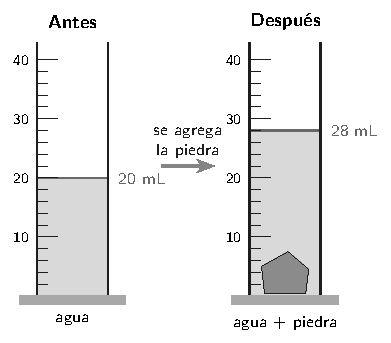
\includegraphics[max width=0.92\linewidth,max height=8.5cm]{qui/atomo_probeta}
\end{center}
 
\begin{ojo}[{Error típico}] Dividir por el volumen final (28 mL) o por el inicial (20 mL). El volumen del sólido es la \textbf{diferencia} entre las dos lecturas.\end{ojo}
 
\begin{clave}[{Precisión}] La probeta mide el volumen con menos precisión que la balanza mide la masa. Con volúmenes pequeños (1 o 2 mL), un error de lectura de 0,1 mL cambia mucho la densidad calculada.\end{clave}
\subsection{Flotación y gráficos de masa y volumen}
\textbf{Flotación.} Un objeto flota en un líquido si su densidad es \textbf{menor} que la del líquido, y se hunde si es mayor. Por eso el hielo (0,92 g/cm\textsuperscript{3}) flota en el agua y una moneda de cobre se hunde. Un huevo se hunde en agua, pero flota en agua con mucha sal: la sal disuelta aumenta la densidad del líquido.

 

Si se juntan líquidos que no se mezclan, se ordenan en capas: el más denso abajo y el menos denso arriba.

 

\textbf{Gráfico de masa versus volumen.} Para una sustancia, la masa es proporcional al volumen: el gráfico es una recta que pasa por el origen, y su \textbf{pendiente es la densidad}. Para leerla, elige un punto de la recta y divide masa por volumen. Mientras más inclinada la recta, mayor la densidad.

  
\begin{center}
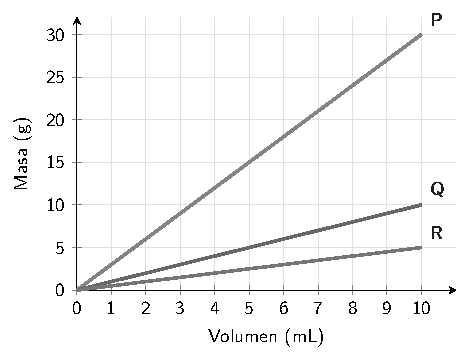
\includegraphics[max width=0.92\linewidth,max height=8.5cm]{qui/atomo_mv_1}
\end{center}
 
\begin{ejemplo}[{Ejemplo resuelto}] En el gráfico, P pasa por (10 mL, 30 g): $d = \dfrac{30}{10} = 3$ g/mL. Q pasa por (10 mL, 10 g): $d = 1$ g/mL, como el agua. R pasa por (10 mL, 5 g): $d = 0{,}5$ g/mL, así que R flota en agua y P se hunde.\end{ejemplo}
 
\begin{ojo}[{Ojo}] La densidad cambia con la temperatura: casi todas las sustancias se dilatan al calentarse, así que su densidad baja un poco. Por eso las tablas indican a qué temperatura se midió.\end{ojo}
\subsection{Temperaturas de fusión y ebullición}
\textbf{Temperatura de fusión:} a la que un sólido pasa a líquido (es la misma a la que el líquido se solidifica). Agua: 0 °C.

 

\textbf{Temperatura de ebullición:} a la que un líquido hierve y pasa a gas (es la misma a la que el gas se condensa). Agua: 100 °C a 1 atm. Depende de la presión: en la cordillera, con menos presión, el agua hierve a menos de 100 °C.

 

\textbf{¿En qué estado está una sustancia a una temperatura T?} Compara T con sus dos temperaturas:

 
\begin{itemize}
  \item T menor que la de fusión \ensuremath{\rightarrow} \textbf{sólido}.
  \item T entre la de fusión y la de ebullición \ensuremath{\rightarrow} \textbf{líquido}.
  \item T mayor que la de ebullición \ensuremath{\rightarrow} \textbf{gas}.
\end{itemize}
  
\begin{ejemplo}[{Ejemplo resuelto}] A 25 °C y 1 atm:
\begin{center}\small
\begin{tabular}{@{}llll@{}}
\toprule
\textbf{Elemento} & \textbf{Fusión (°C)} & \textbf{Ebullición (°C)} & \textbf{Estado} \\
\midrule
Cloro & \ensuremath{-}101 & \ensuremath{-}35 & gas (25 > \ensuremath{-}35) \\
Bromo & \ensuremath{-}7 & 59 & líquido (\ensuremath{-}7 < 25 < 59) \\
Yodo & 114 & 184 & sólido (25 < 114) \\
\bottomrule
\end{tabular}
\end{center}\end{ejemplo}
 
\begin{ojo}[{Error típico con negativos}] \ensuremath{-}35 °C es una temperatura \textbf{más baja} que 25 °C. Si la temperatura de ebullición es negativa, a temperatura ambiente la sustancia ya hirvió: es un gas.\end{ojo}
\subsection{Curvas de calentamiento}
Si se calienta una sustancia y se anota la temperatura cada minuto, se obtiene una \textbf{curva de calentamiento}.

 
\begin{itemize}
  \item En los tramos inclinados, la sustancia está en un solo estado y su temperatura sube.
  \item En los tramos horizontales (\textbf{mesetas}) ocurre un cambio de estado: la sustancia sigue recibiendo calor, pero esa energía se usa en separar las partículas y la temperatura no sube. La primera meseta es la \textbf{fusión} (sólido y líquido juntos) y la segunda, la \textbf{ebullición} (líquido y gas juntos).
\end{itemize}
 

\textbf{Sustancia pura o mezcla.} Una sustancia pura tiene mesetas planas: funde y hierve a una temperatura fija. Una mezcla funde y hierve en un \textbf{rango} de temperaturas: la «meseta» queda inclinada, porque la composición del líquido va cambiando mientras hierve.

  
\begin{center}
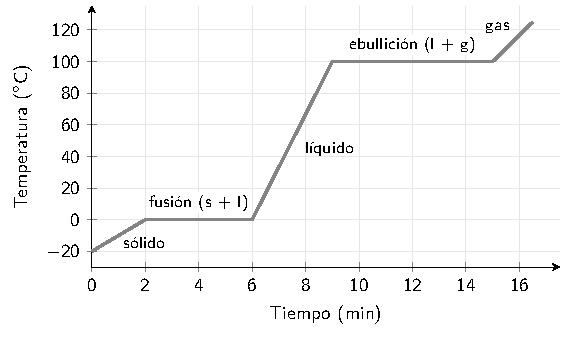
\includegraphics[max width=0.92\linewidth,max height=8.5cm]{qui/atomo_calentamiento}
\end{center}
 
\begin{center}
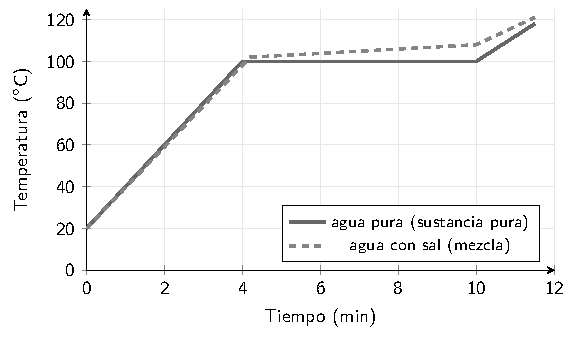
\includegraphics[max width=0.92\linewidth,max height=8.5cm]{qui/atomo_pura_mezcla}
\end{center}
\subsection{Lo clave del tema}
\begin{center}\small
\begin{tabularx}{\linewidth}{@{}>{\raggedright\arraybackslash\hsize=0.97\hsize}X>{\raggedright\arraybackslash\hsize=0.47\hsize}X>{\raggedright\arraybackslash\hsize=1.56\hsize}X@{}}
\toprule
\textbf{Propiedad} & \textbf{Tipo} & \textbf{Cómo se mide o calcula} \\
\midrule
Masa & extensiva & balanza (g) \\
Volumen & extensiva & probeta; sólidos irregulares, desplazamiento de agua (mL = cm\textsuperscript{3}) \\
Densidad & intensiva & $d = \dfrac{m}{V}$; pendiente del gráfico masa-volumen \\
Temperatura de fusión & intensiva & primera meseta de la curva de calentamiento \\
Temperatura de ebullición & intensiva & segunda meseta; depende de la presión \\
\bottomrule
\end{tabularx}
\end{center}
 
\begin{clave}[{Recuerda}] · La densidad es intensiva: si partes un objeto, no cambia.\par · $m = d\cdot V$ (revisa las unidades).\par · Volumen de la piedra = lectura final \ensuremath{-} lectura inicial.\par · En la meseta el calor que entra se usa en el cambio de estado.\par · Si una sustancia hierve a \ensuremath{-}35 °C, a 25 °C ya es gas.\end{clave}
 
\begin{clave}[{Método PAES}] 1. Anota los datos con sus unidades. 2. Elige la fórmula: $d = \dfrac{m}{V}$, $m = d\cdot V$ o $V = \dfrac{m}{d}$. 3. Revisa que las unidades den lo pedido. 4. Para el estado físico, ubica la temperatura entre la de fusión y la de ebullición. 5. En gráficos, lee primero los ejes y sus unidades; en tablas de datos, busca qué variable cambia junto con cuál.\end{clave}
\begin{elejemplo}{PAES Invierno 2027, adaptada}
Como parte de un proyecto escolar, un grupo de estudiantes midió la masa y el volumen de cinco muestras de cobre refinado, que la empresa minera etiqueta con una pureza de 99,99 \%. Con esos valores calcularon la densidad de cada muestra y la compararon con el valor de referencia del cobre, 8,96 g/cm\textsuperscript{3}. Todas las mediciones se hicieron con la misma balanza y la misma probeta, en una sala a temperatura constante:

La profesora les comenta que el trabajo tiene un problema de confiabilidad. ¿Cuál de los siguientes factores lo perjudicó?
\begin{center}\small
\begin{tabularx}{\linewidth}{@{}>{\raggedright\arraybackslash\hsize=0.57\hsize}X>{\raggedright\arraybackslash\hsize=0.51\hsize}X>{\raggedright\arraybackslash\hsize=1.37\hsize}X>{\raggedright\arraybackslash\hsize=1.54\hsize}X@{}}
\toprule
\textbf{Muestra} & \textbf{Masa (g)} & \textbf{Volumen (cm\textsuperscript{3})} & \textbf{Densidad (g/cm\textsuperscript{3})} \\
\midrule
\textbf{1} & 17,204 & 2,0 & 8,6 \\
\textbf{2} & 9,398 & 1,0 & 9,4 \\
\textbf{3} & 13,653 & 1,5 & 9,1 \\
\textbf{4} & 16,998 & 2,0 & 8,5 \\
\textbf{5} & 8,803 & 1,0 & 8,8 \\
\bottomrule
\end{tabularx}
\end{center}
\altslargas{La cantidad de muestras utilizadas.}{Los valores de volumen registrados.}{El uso de un valor de densidad de referencia.}{La procedencia de las muestras desde una empresa.}
\solucion{\textbf{Paso 1. ¿Qué nos piden?} Encontrar qué parte del trabajo hace que los resultados no sean confiables. Primero vemos si los datos tienen sentido.

\textbf{Paso 2. Revisa los cálculos.} $\dfrac{17{,}204}{2{,}0} = 8{,}6$; $\dfrac{9{,}398}{1{,}0} = 9{,}4$; $\dfrac{13{,}653}{1{,}5} = 9{,}1$; $\dfrac{16{,}998}{2{,}0} = 8{,}5$; $\dfrac{8{,}803}{1{,}0} = 8{,}8$. Las cuentas están bien hechas.

\textbf{Paso 3. ¿Qué esperábamos?} Las cinco muestras son del mismo cobre, casi puro. La densidad es intensiva: todas deberían dar casi lo mismo, cerca de 8,96 g/cm\textsuperscript{3}. Pero los resultados van de 8,5 a 9,4: varían demasiado.

\textbf{Paso 4. Busca la causa.} Las masas tienen tres decimales: la balanza es muy precisa. Los volúmenes tienen un solo decimal y son muy pequeños (1 o 2 cm\textsuperscript{3}), medidos con una probeta. Un error de lectura de solo 0,1 cm\textsuperscript{3} en 1,0 cm\textsuperscript{3} es un error del 10 \% en la densidad. Por ejemplo, la muestra 2 daría $\dfrac{9{,}398}{1{,}05} \approx 8{,}95$ g/cm\textsuperscript{3} si su volumen real fuera 1,05 cm\textsuperscript{3}, en vez de 1,0.

\textbf{Respuesta:} los valores de volumen registrados.

\textbf{Comprobación:} si el problema fuera la pureza, todas las densidades se correrían hacia el mismo lado; aquí unas quedan sobre 8,96 y otras bajo 8,96, que es lo típico de un error de medición al azar.

\textbf{¿Por qué no las otras?} Cinco muestras es una cantidad razonable; más muestras no arreglan una medición imprecisa. Comparar con un valor de referencia es justamente lo que permite detectar el problema. Que las muestras vengan de una empresa no afecta la medición: el cobre está etiquetado con 99,99 \% de pureza.

\textbf{\color{cienciaD}Para recordar.} Si una muestra pura da densidades muy distintas, revisa la precisión de las mediciones, sobre todo de los volúmenes pequeños.}{B}
\end{elejemplo}

%% =====================================================================
%% qui_modelos
\section[Modelos atómicos: de Dalton a Bohr]{Modelos atómicos: de Dalton a Bohr}
\modcomun\ \ {\color{gris}\itshape La teoría de Dalton y los modelos de Thomson, Rutherford y Bohr: qué propuso cada uno, qué experimento u observación lo motivó, qué explicó, cuáles fueron sus limitaciones y en qué orden aparecieron.\par}
\subsection{Por qué hay varios modelos atómicos}
Nadie ha visto un átomo a simple vista. Un \textbf{modelo atómico} es una representación que explica lo que se observa en los experimentos. Cuando aparece una observación que el modelo no puede explicar, se propone uno nuevo que sí la explique.

 

Así, cada modelo corrige al anterior:

 
\begin{center}\small
\begin{tabularx}{\linewidth}{@{}>{\raggedright\arraybackslash\hsize=0.72\hsize}X>{\raggedright\arraybackslash\hsize=0.81\hsize}X>{\raggedright\arraybackslash\hsize=1.48\hsize}X@{}}
\toprule
\textbf{Año} & \textbf{Modelo} & \textbf{Idea central} \\
\midrule
1808 & Dalton & átomos indivisibles \\
1897--1904 & Thomson & el átomo tiene electrones \\
1911 & Rutherford & núcleo pequeño, positivo y denso \\
1913 & Bohr & niveles de energía \\
1926 en adelante & mecano-cuántico & orbitales (zonas de probabilidad) \\
\bottomrule
\end{tabularx}
\end{center}
  
\gatotip[\gatogris]{\textbf{Para recordar el orden.} Cada modelo agrega algo «más adentro» del átomo: Dalton (el átomo entero) \ensuremath{\rightarrow} Thomson (sus electrones) \ensuremath{\rightarrow} Rutherford (su núcleo) \ensuremath{\rightarrow} Bohr (la energía de los electrones).}
  
\begin{center}
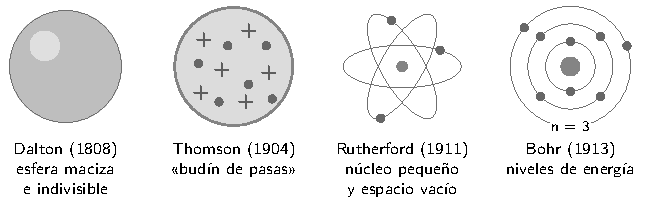
\includegraphics[max width=0.92\linewidth,max height=8.5cm]{qui/atomo_modelos}
\end{center}
\subsection{Dalton: el átomo indivisible}
John Dalton (1808) propuso la primera teoría atómica con base experimental. Sus postulados:

 
\begin{itemize}
  \item La materia está formada por partículas muy pequeñas e \textbf{indivisibles}: los átomos.
  \item Los átomos de un mismo elemento son \textbf{iguales} entre sí (misma masa y propiedades) y distintos de los de otros elementos.
  \item Los compuestos se forman al combinarse átomos de distintos elementos en \textbf{proporciones de números enteros sencillos}.
  \item En una reacción química los átomos \textbf{se reordenan}: no se crean ni se destruyen.
\end{itemize}
 

Con esto explicó la ley de conservación de la masa y la ley de las proporciones definidas.

  
\begin{ojo}[{Limitaciones}] El átomo \textbf{sí es divisible}: tiene electrones, protones y neutrones. Y no todos los átomos de un elemento tienen la misma masa: existen los \textbf{isótopos}. Su modelo no dice nada sobre cargas eléctricas.\end{ojo}
 
\begin{ejemplo}[{Ejemplo resuelto}] ¿Qué postulado de Dalton explica que en una reacción la masa total no cambie? El último: los átomos solo se reordenan. Si hay los mismos átomos antes y después, la masa es la misma.\end{ejemplo}
\subsection{Thomson: el descubrimiento del electrón}
J. J. Thomson trabajó con \textbf{tubos de rayos catódicos}: tubos de vidrio casi sin aire, con un metal en cada extremo conectado a alto voltaje. Desde el polo negativo salía un rayo que se desviaba hacia una placa con carga \textbf{positiva}.

 

\textbf{Conclusión:} el rayo está formado por partículas con \textbf{carga negativa}, mucho más livianas que un átomo, y aparecen con cualquier metal. Esas partículas, los \textbf{electrones}, forman parte de todos los átomos. Por lo tanto, el átomo \textbf{no es indivisible}.

 

\textbf{Modelo del «budín de pasas»} (1904): el átomo es una esfera con carga positiva repartida de manera uniforme, y los electrones están incrustados en ella, como pasas en un budín. Las cargas positivas y negativas se compensan: el átomo es neutro.

  
\begin{ojo}[{Limitación}] Con la carga positiva repartida por toda la esfera, ninguna partícula debería rebotar al chocar con un átomo. El experimento de Rutherford mostró lo contrario.\end{ojo}
 
\begin{clave}[{Error típico}] «Thomson descubrió el núcleo». No: Thomson descubrió el \textbf{electrón}. El núcleo lo propuso Rutherford.\end{clave}
\subsection{Rutherford: el experimento de la lámina de oro}
En 1911, el equipo de Ernest Rutherford bombardeó una lámina de oro muy delgada con \textbf{partículas alfa} (partículas con carga positiva) y registró hacia dónde salían en una pantalla.

 
\begin{center}\small
\begin{tabularx}{\linewidth}{@{}>{\raggedright\arraybackslash\hsize=1.00\hsize}X>{\raggedright\arraybackslash\hsize=1.00\hsize}X@{}}
\toprule
\textbf{Observación} & \textbf{Conclusión} \\
\midrule
Casi todas pasan sin desviarse & el átomo es casi todo \textbf{espacio vacío} \\
Algunas se desvían & hay una zona con carga \textbf{positiva} que las repele \\
Muy pocas (1 de cada 10.000 a 100.000) rebotan & esa zona es muy \textbf{pequeña} y muy \textbf{densa}: concentra casi toda la masa \\
\bottomrule
\end{tabularx}
\end{center}
 

\textbf{Modelo nuclear} (o planetario): un \textbf{núcleo} diminuto, positivo, con casi toda la masa del átomo, y los electrones girando alrededor, lejos de él. Si el átomo fuera un estadio, el núcleo sería una bolita en el centro de la cancha.

  
\begin{ojo}[{Limitación}] Según la física de la época, un electrón que gira debería emitir energía, perder velocidad y caer en espiral al núcleo: el átomo no sería estable. Tampoco explicaba por qué cada elemento emite luz solo de ciertos colores.\end{ojo}
  
\begin{center}
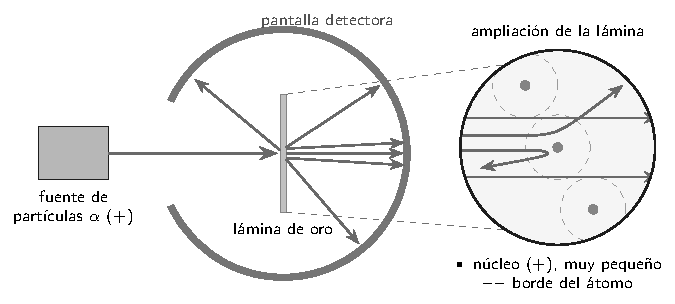
\includegraphics[max width=0.92\linewidth,max height=8.5cm]{qui/atomo_rutherford}
\end{center}
\subsection{Bohr: los niveles de energía}
Niels Bohr (1913) mantuvo el núcleo de Rutherford y agregó reglas para los electrones:

 
\begin{itemize}
  \item Los electrones giran en \textbf{órbitas circulares} de radio y \textbf{energía fijos}, llamadas niveles ($n = 1, 2, 3$\dots{}). Mientras está en su nivel, el electrón no pierde energía.
  \item Mientras más lejos del núcleo, \textbf{mayor es la energía} del nivel y \textbf{menor la energía que se necesita para arrancar} el electrón del átomo.
  \item Un electrón \textbf{absorbe} energía y salta a un nivel más alejado. Al volver a un nivel más cercano, \textbf{emite} esa energía como luz.
\end{itemize}
 

Como los niveles tienen energías fijas, solo se emiten ciertas energías, es decir, ciertos colores: el \textbf{espectro de líneas} de cada elemento. Por eso el sodio da luz amarilla y el cobre, verde, en el ensayo a la llama y en los fuegos artificiales.

  
\begin{clave}[{En los diagramas de la PAES}] Para los primeros 20 elementos, los electrones se ubican así: hasta 2 en el primer nivel, hasta 8 en el segundo y hasta 8 en el tercero.\end{clave}
 
\begin{ojo}[{Limitación}] Funciona muy bien para el hidrógeno, pero no para átomos con muchos electrones. El modelo actual (mecano-cuántico) reemplaza las órbitas por \textbf{orbitales}: zonas donde es más probable encontrar al electrón.\end{ojo}
  
\begin{center}
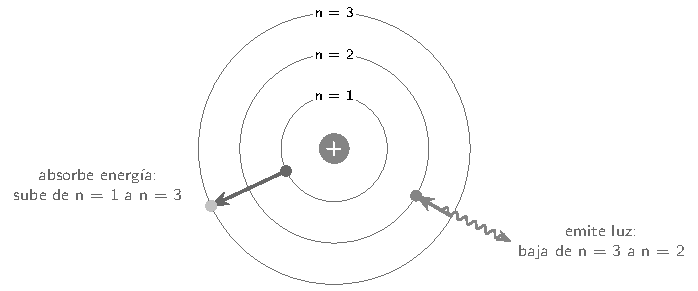
\includegraphics[max width=0.92\linewidth,max height=8.5cm]{qui/atomo_bohr}
\end{center}
\subsection{Lo clave del tema}
\begin{center}\small
\begin{tabularx}{\linewidth}{@{}>{\raggedright\arraybackslash\hsize=0.52\hsize}X>{\raggedright\arraybackslash\hsize=1.04\hsize}X>{\raggedright\arraybackslash\hsize=1.22\hsize}X>{\raggedright\arraybackslash\hsize=1.22\hsize}X@{}}
\toprule
\textbf{Modelo} & \textbf{Evidencia} & \textbf{Qué aporta} & \textbf{Limitación} \\
\midrule
Dalton (1808) & leyes de la masa en las reacciones & átomos indivisibles que se reordenan & el átomo es divisible; hay isótopos \\
Thomson (1904) & rayos catódicos & electrones (\ensuremath{-}) en una esfera positiva & no explica los rebotes de partículas alfa \\
Rutherford (1911) & lámina de oro y partículas alfa & núcleo pequeño, denso y positivo; espacio vacío & el electrón caería al núcleo; no explica los espectros \\
Bohr (1913) & espectros de líneas & niveles de energía fijos; absorción y emisión & solo funciona bien para el hidrógeno \\
\bottomrule
\end{tabularx}
\end{center}
 
\begin{clave}[{Recuerda}] · Thomson descubrió el electrón; Rutherford propuso el núcleo.\par · Casi todas las partículas alfa pasan derecho porque el átomo es casi vacío; unas pocas rebotan al chocar con el núcleo, denso y positivo.\par · Las partículas alfa se desvían por la repulsión del núcleo positivo; los electrones son muy livianos para desviarlas.\par · El electrón absorbe energía al subir de nivel y emite luz al bajar.\par · Los electrones más lejanos son los más fáciles de arrancar.\end{clave}
 
\begin{clave}[{Método PAES}] 1. Identifica de qué modelo habla el texto por su experimento o su idea clave (rayos catódicos \ensuremath{\rightarrow} Thomson; lámina de oro \ensuremath{\rightarrow} Rutherford; niveles y espectros \ensuremath{\rightarrow} Bohr). 2. Une cada observación con la conclusión que permite. 3. Descarta las alternativas que mezclan ideas de modelos distintos o que son ciertas pero no salen de lo descrito.\end{clave}
\begin{elejemplo}{PAES Invierno 2026, adaptada}
A comienzos del siglo XX, un científico propuso un modelo atómico formado por un núcleo y electrones girando a su alrededor. El modelo surgió de un experimento en el que se lanzaron partículas alfa, de carga positiva, contra una lámina muy delgada de oro:

La gran mayoría de las partículas atravesó la lámina sin cambiar su trayectoria. Unas pocas se desviaron y, aproximadamente, una de cada cien mil rebotó en dirección contraria.

De acuerdo con lo anterior, ¿cuál de las siguientes inferencias es correcta?
\begin{center}
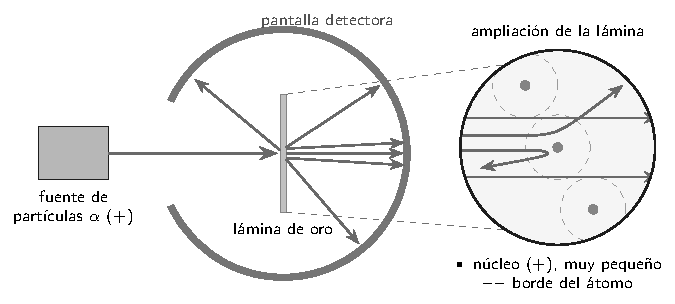
\includegraphics[max width=0.92\linewidth,max height=8.5cm]{qui/atomo_rutherford}
\end{center}
\altslargas{El átomo tiene un núcleo que ocupa casi todo su volumen.}{Los electrones del átomo repelen a las partículas alfa.}{El átomo está formado principalmente por espacio vacío.}{El núcleo del átomo tiene carga negativa.}
\solucion{\textbf{Paso 1. ¿Qué nos piden?} Una inferencia que se apoye en las observaciones del experimento de Rutherford. Unimos cada observación con lo que permite concluir.

\textbf{Paso 2. «La gran mayoría pasa sin desviarse».} Si casi todas las partículas atraviesan los miles de capas de átomos de la lámina sin chocar con nada, dentro del átomo casi no hay nada que se interponga: el átomo es principalmente \textbf{espacio vacío}.

\textbf{Paso 3. «Unas pocas se desvían».} Las partículas alfa son positivas. Si algo las desvía, es una zona con carga \textbf{positiva} que las repele.

\textbf{Paso 4. «Una de cada cien mil rebota».} Para hacer rebotar a una partícula tan rápida, esa zona tiene que ser muy densa. Y como casi nunca se choca con ella, debe ser muy pequeña: es el núcleo.

\textbf{Respuesta:} el átomo está formado principalmente por espacio vacío.

\textbf{Comprobación:} si el núcleo fuera grande, muchas partículas chocarían con él y rebotarían; pero rebota solo 1 de cada 100.000, así que el núcleo ocupa una parte ínfima del volumen.

\textbf{¿Por qué no las otras?} «Un núcleo que ocupa casi todo el volumen» contradice que casi todas las partículas pasen. Los electrones tienen carga negativa: atraerían a las partículas alfa, no las repelerían, y además son tan livianos que no pueden desviarlas. Un núcleo negativo atraería a las partículas alfa; no las haría rebotar.

\textbf{\color{cienciaD}Para recordar.} Pasan derecho \ensuremath{\rightarrow} espacio vacío. Se desvían o rebotan \ensuremath{\rightarrow} núcleo pequeño, denso y positivo.}{C}
\end{elejemplo}

%% =====================================================================
%% qui_particulas
\section[Protones, neutrones y electrones]{Protones, neutrones y electrones}
\modcomun\ \ {\color{gris}\itshape Las partículas del átomo, el número atómico Z y el número másico A, la notación de núclido, los isótopos y los iones (cationes y aniones), y cómo contar protones, neutrones y electrones en símbolos y diagramas.\par}
\subsection{Las tres partículas del átomo}
Todo átomo tiene un \textbf{núcleo} muy pequeño, con protones y neutrones, y alrededor, los \textbf{electrones}.

 
\begin{center}\small
\begin{tabular}{@{}llll@{}}
\toprule
\textbf{Partícula} & \textbf{Carga} & \textbf{Masa relativa} & \textbf{Ubicación} \\
\midrule
Protón (p\textsuperscript{+}) & +1 & 1 u & núcleo \\
Neutrón (n\textsuperscript{0}) & 0 & 1 u & núcleo \\
Electrón (e\textsuperscript{\ensuremath{-}}) & \ensuremath{-}1 & casi 0 (1/1840 u) & niveles, fuera del núcleo \\
\bottomrule
\end{tabular}
\end{center}
 

Dos consecuencias:

 
\begin{itemize}
  \item La \textbf{masa} del átomo está casi toda en el núcleo: protones y neutrones.
  \item La \textbf{carga} depende de protones y electrones. Si hay tantos electrones como protones, las cargas se anulan y el átomo es \textbf{neutro}.
\end{itemize}
  
\begin{center}
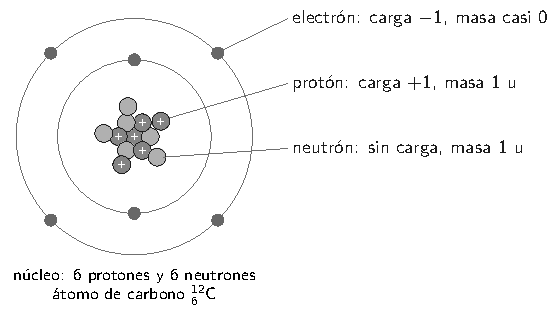
\includegraphics[max width=0.92\linewidth,max height=8.5cm]{qui/atomo_partes}
\end{center}
 
\begin{ojo}[{Ojo}] Los neutrones no tienen carga, pero sí masa: cuentan para la masa del átomo y no cuentan para su carga.\end{ojo}
\subsection{Número atómico Z y número másico A}
\textbf{Número atómico (Z):} la cantidad de \textbf{protones}. Es el «carnet de identidad» del elemento: todos los átomos de carbono tienen 6 protones, y cualquier átomo con 6 protones es carbono. La tabla periódica ordena los elementos según Z.

 

\textbf{Número másico (A):} la cantidad de \textbf{protones más neutrones}, las partículas del núcleo.

 \[ A = Z + n \qquad\Rightarrow\qquad n = A - Z \] 

\textbf{Notación de núclido:} A arriba a la izquierda, Z abajo a la izquierda y la carga, si la hay, arriba a la derecha: $\,{}^{A}_{Z}\text{X}^{\text{carga}}$.

 

En un átomo \textbf{neutro}, electrones = protones = Z.

  
\begin{ejemplo}[{Ejemplo resuelto}] $\,{}^{23}_{11}\text{Na}$.\par \textbf{Paso 1.} Protones: Z = 11.\par \textbf{Paso 2.} Neutrones: $23 - 11 = 12$.\par \textbf{Paso 3.} Electrones: no tiene carga, así que es neutro: 11.\end{ejemplo}
 
\begin{ojo}[{Error típico}] Confundir Z con A, o creer que los neutrones son iguales a los protones. En $\,{}^{35}_{17}\text{Cl}$ hay 17 protones y $35 - 17 = 18$ neutrones.\end{ojo}
 
\begin{clave}[{Masa atómica de la tabla}] No es un número entero (Cl = 35,5) porque es un promedio de los isótopos naturales del elemento. El número másico A, en cambio, siempre es entero.\end{clave}
\subsection{Iones: cationes y aniones}
Un \textbf{ion} es un átomo (o grupo de átomos) con carga eléctrica, porque \textbf{ganó o perdió electrones}. Los protones no cambian: siguen siendo los mismos, y por eso el elemento sigue siendo el mismo.

 
\begin{itemize}
  \item \textbf{Catión} (carga +): \textbf{perdió} electrones. Na\textsuperscript{+}: 11 protones y 10 electrones.
  \item \textbf{Anión} (carga \ensuremath{-}): \textbf{ganó} electrones. Cl\textsuperscript{\ensuremath{-}}: 17 protones y 18 electrones.
\end{itemize}
 

La regla para contar electrones:

 \[ \text{electrones} = Z - \text{carga} \] 

Con carga 2+: $Z - 2$. Con carga 2\ensuremath{-}: $Z - (-2) = Z + 2$.

  
\begin{ejemplo}[{Ejemplo resuelto}] $\,{}^{40}_{20}\text{Ca}^{2+}$.\par \textbf{Paso 1.} Protones: 20.\par \textbf{Paso 2.} Neutrones: $40 - 20 = 20$.\par \textbf{Paso 3.} Electrones: carga 2+, perdió 2: $20 - 2 = 18$.\end{ejemplo}
 
\begin{ejemplo}[{Ejemplo resuelto}] $\,{}^{32}_{16}\text{S}^{2-}$: 16 protones, $32 - 16 = 16$ neutrones y $16 + 2 = 18$ electrones.\end{ejemplo}
 
\begin{ojo}[{Error típico}] «El catión ganó protones». No: un ion nunca cambia sus protones. Si cambiaran los protones, sería otro elemento. Y el signo engaña: carga + significa \textbf{menos} electrones.\end{ojo}
\subsection{Isótopos, isóbaros e isótonos}
\textbf{Isótopos:} átomos del \textbf{mismo elemento} (igual Z) con distinto número de neutrones y, por eso, distinto A. Tienen las mismas propiedades químicas, porque tienen los mismos protones y electrones; solo cambia su masa.

 
\begin{itemize}
  \item Carbono: $\,{}^{12}_{6}\text{C}$ (6 n), $\,{}^{13}_{6}\text{C}$ (7 n) y $\,{}^{14}_{6}\text{C}$ (8 n). El carbono 14 se usa para datar restos arqueológicos.
  \item Hidrógeno: protio $\,{}^{1}_{1}\text{H}$ (0 n), deuterio $\,{}^{2}_{1}\text{H}$ (1 n) y tritio $\,{}^{3}_{1}\text{H}$ (2 n).
\end{itemize}
 

La PAES a veces define otras dos palabras en el enunciado:

 
\begin{itemize}
  \item \textbf{Isóbaros:} igual A, distinto Z (elementos distintos): $\,{}^{40}_{18}\text{Ar}$ y $\,{}^{40}_{20}\text{Ca}$.
  \item \textbf{Isótonos:} igual número de neutrones: $\,{}^{39}_{19}\text{K}$ y $\,{}^{40}_{20}\text{Ca}$ (20 n cada uno).
\end{itemize}
  
\begin{center}\small
\begin{tabular}{@{}llll@{}}
\toprule
\textbf{Comparación} & \textbf{Z (protones)} & \textbf{A} & \textbf{Neutrones} \\
\midrule
Isótopos & igual & distinto & distinto \\
Isóbaros & distinto & igual & distinto \\
Isótonos & distinto & distinto & igual \\
\bottomrule
\end{tabular}
\end{center}
 
\begin{ejemplo}[{Ejemplo resuelto}] ¿En qué se diferencian $\,{}^{28}_{14}\text{Si}$, $\,{}^{29}_{14}\text{Si}$ y $\,{}^{30}_{14}\text{Si}$? Tienen igual Z (14 protones) y, como son neutros, 14 electrones. Se diferencian en los neutrones: 14, 15 y 16. Son isótopos.\end{ejemplo}
\subsection{Contar partículas en un diagrama}
En la PAES aparecen diagramas de Bohr con el núcleo y los electrones dibujados como puntos en sus niveles. Para leerlos:

 

\textbf{Paso 1.} Lee en el núcleo los protones (p) y los neutrones (n).

 

\textbf{Paso 2.} Cuenta los electrones de todos los niveles.

 

\textbf{Paso 3.} Compara: si hay más electrones que protones, es un anión; si hay menos, un catión; si son iguales, un átomo neutro.

 

\textbf{Paso 4.} Arma la notación: Z = protones, A = protones + neutrones, carga = protones \ensuremath{-} electrones.

 

Si el diagrama muestra solo neutrones y dice que el átomo es neutro, los protones son iguales a los electrones que cuentas.

  
\begin{center}
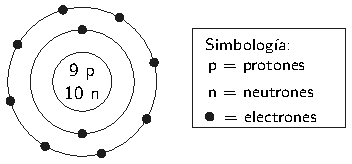
\includegraphics[max width=0.92\linewidth,max height=8.5cm]{qui/atomo_fluoruro}
\end{center}
 
\begin{ejemplo}[{Ejemplo resuelto}] En el diagrama: 9 p y 10 n en el núcleo; electrones: $2 + 8 = 10$. Z = 9, A = 9 + 10 = 19 y carga = 9 \ensuremath{-} 10 = \ensuremath{-}1. Es $\,{}^{19}_{9}\text{X}^{-}$: el ion fluoruro, F\textsuperscript{\ensuremath{-}}.\end{ejemplo}
\subsection{Lo clave del tema}
\begin{center}\small
\begin{tabularx}{\linewidth}{@{}>{\raggedright\arraybackslash\hsize=0.72\hsize}X>{\raggedright\arraybackslash\hsize=0.67\hsize}X>{\raggedright\arraybackslash\hsize=1.61\hsize}X@{}}
\toprule
\textbf{Quiero saber} & \textbf{Cómo lo calculo} & \textbf{Ejemplo: $\,{}^{56}_{26}\text{Fe}^{3+}$} \\
\midrule
Protones & Z & 26 \\
Neutrones & A \ensuremath{-} Z & 56 \ensuremath{-} 26 = 30 \\
Electrones & Z \ensuremath{-} carga & 26 \ensuremath{-} 3 = 23 \\
¿Mismo elemento? & mismo Z & todo átomo con 26 protones es hierro \\
\bottomrule
\end{tabularx}
\end{center}
 
\begin{clave}[{Recuerda}] · Neutrones = A \ensuremath{-} Z.\par · Una carga positiva indica electrones perdidos: Fe\textsuperscript{3+} tiene 26 \ensuremath{-} 3 = 23 electrones.\par · En un ion solo cambian los electrones; los protones definen el elemento.\par · Los isótopos tienen igual Z y distinto número de neutrones.\par · Neutrones y protones pueden ser distintos: $\,{}^{35}_{17}\text{Cl}$ tiene 18 neutrones.\end{clave}
 
\begin{clave}[{Método PAES}] 1. Haz una tablita con p, n y e de cada especie antes de leer las alternativas. 2. Protones = Z; neutrones = A \ensuremath{-} Z; electrones = Z \ensuremath{-} carga. 3. Para comparar especies, resta fila por fila. 4. Para «mismo elemento» o «isótopos», mira solo Z.\end{clave}
\begin{elejemplo}{PAES Invierno 2026, adaptada}
La siguiente tabla presenta el número de protones de cuatro iones:

A partir de la tabla, ¿cuál de las siguientes comparaciones del número de electrones de los iones es correcta?
\begin{center}\small
\begin{tabular}{@{}ll@{}}
\toprule
\textbf{Ion} & \textbf{N.° de protones} \\
\midrule
\textbf{I\textsuperscript{\ensuremath{-}}} & 53 \\
\textbf{S\textsuperscript{2\ensuremath{-}}} & 16 \\
\textbf{Mg\textsuperscript{2+}} & 12 \\
\textbf{Al\textsuperscript{3+}} & 13 \\
\bottomrule
\end{tabular}
\end{center}
\altslargas{El ion S\textsuperscript{2\ensuremath{-}} tiene 4 electrones más que el ion Mg\textsuperscript{2+}.}{El ion Mg\textsuperscript{2+} tiene 1 electrón menos que el ion Al\textsuperscript{3+}.}{El ion I\textsuperscript{\ensuremath{-}} tiene 36 electrones más que el ion S\textsuperscript{2\ensuremath{-}}.}{El ion Al\textsuperscript{3+} tiene 40 electrones menos que el ion I\textsuperscript{\ensuremath{-}}.}
\solucion{\textbf{Paso 1. ¿Qué nos piden?} Comparar electrones, pero la tabla da protones. Primero calculamos los electrones de cada ion con electrones = protones \ensuremath{-} carga.

\textbf{Paso 2. I\textsuperscript{\ensuremath{-}}.} Carga \ensuremath{-}1: ganó 1 electrón. $53 + 1 = 54$ electrones.

\textbf{Paso 3. S\textsuperscript{2\ensuremath{-}}.} Ganó 2: $16 + 2 = 18$ electrones.

\textbf{Paso 4. Mg\textsuperscript{2+}.} Perdió 2: $12 - 2 = 10$ electrones.

\textbf{Paso 5. Al\textsuperscript{3+}.} Perdió 3: $13 - 3 = 10$ electrones.

\textbf{Paso 6. Compara.} I\textsuperscript{\ensuremath{-}} y S\textsuperscript{2\ensuremath{-}}: $54 - 18 = 36$. \ding{52} S\textsuperscript{2\ensuremath{-}} y Mg\textsuperscript{2+}: $18 - 10 = 8$. Mg\textsuperscript{2+} y Al\textsuperscript{3+}: $10 - 10 = 0$, tienen los mismos. Al\textsuperscript{3+} y I\textsuperscript{\ensuremath{-}}: $54 - 10 = 44$.

\textbf{Respuesta:} el ion I\textsuperscript{\ensuremath{-}} tiene 36 electrones más que el ion S\textsuperscript{2\ensuremath{-}}.

\textbf{Comprobación:} I\textsuperscript{\ensuremath{-}} tiene los mismos electrones que el gas noble xenón (54) y S\textsuperscript{2\ensuremath{-}}, los mismos que el argón (18): $54 - 18 = 36$ \ding{52}.

\textbf{¿Por qué no las otras?} Las otras tres comparan \textbf{protones} en vez de electrones, olvidando la carga: $16 - 12 = 4$, $13 - 12 = 1$ y $53 - 13 = 40$. Con los electrones, las diferencias reales son 8, 0 y 44.

\textbf{\color{cienciaD}Para recordar.} Antes de comparar iones, convierte protones en electrones: electrones = Z \ensuremath{-} carga.}{C}
\end{elejemplo}

\chapter{Química orgánica}
%% =====================================================================
%% qui_carbono
\section[El átomo de carbono]{El átomo de carbono}
\modcomun\ \ {\color{gris}\itshape Por qué el carbono forma cuatro enlaces, cómo contar enlaces sigma y pi, cómo reconocer la hibridación sp³, sp² y sp de cada carbono y cómo cambian la energía, la longitud y el ángulo de enlace.\par}
\subsection{Tetravalencia: el carbono siempre forma 4 enlaces}
El carbono tiene $Z = 6$: su configuración es 1s\textsuperscript{2} 2s\textsuperscript{2} 2p\textsuperscript{2}. Tiene \textbf{4 electrones de valencia} y los comparte todos: forma siempre \textbf{4 enlaces covalentes}. A esto se le llama \textbf{tetravalencia}.

 

Los 4 enlaces pueden repartirse de varias formas: cuatro simples, un doble y dos simples, un triple y un simple, o dos dobles. Lo que nunca cambia es la suma: \textbf{4}.

 

Además, el carbono se une fácilmente con otros carbonos (\textbf{concatenación}): forma cadenas largas, ramificadas y anillos. Por eso existen millones de compuestos orgánicos.

 
\begin{center}\small
\begin{tabular}{@{}ll@{}}
\toprule
\textbf{Átomo} & \textbf{N.º de enlaces que forma} \\
\midrule
C & 4 \\
N & 3 \\
O, S & 2 \\
H, F, Cl, Br, I & 1 \\
\bottomrule
\end{tabular}
\end{center}
  
\begin{ejemplo}[{Ejemplo: revisa una estructura}] En CH\textsubscript{2}=CH--CH\textsubscript{3} (propeno):\par · C1: doble (cuenta 2) + 2 H = 4 \ding{52}\par · C2: doble (2) + 1 H + 1 simple = 4 \ding{52}\par · C3: 1 simple + 3 H = 4 \ding{52}\end{ejemplo}
 
\begin{ojo}[{Error típico}] Contar un enlace doble como 1. Un doble "gasta" 2 de los 4 enlaces del carbono y un triple gasta 3. Por eso el CH de un doble enlace tiene un solo H, y el C de un triple interno no tiene ninguno.\end{ojo}
\subsection{Enlaces simple, doble y triple: sigma y pi}
Cada línea de una fórmula es un par de electrones compartidos. Pero no todos los enlaces son iguales:

 
\begin{itemize}
  \item \textbf{Enlace simple} (C--C, C--H): 1 enlace \textbf{sigma} ($\sigma$).
  \item \textbf{Enlace doble} (C=C, C=O): 1 $\sigma$ + 1 \textbf{pi} ($\pi$).
  \item \textbf{Enlace triple} (C\ensuremath{\equiv}C, C\ensuremath{\equiv}N): 1 $\sigma$ + 2 $\pi$.
\end{itemize}
 

El enlace $\sigma$ une los núcleos de frente; el $\pi$ se forma por los lados, con orbitales p que quedaron sin mezclar. Entre dos átomos hay \textbf{como máximo un} $\sigma$.

 
\begin{clave}[{Método para contar}] 1. Dibuja (o imagina) todos los H. 2. Cada enlace, sea simple, doble o triple, aporta \textbf{exactamente 1} $\sigma$. 3. Los $\pi$ son las líneas extra: 1 por cada doble y 2 por cada triple.\end{clave}
 
\gatotip[\gatonegro]{\textbf{Atajo.} En una molécula sin anillos, n.º de $\sigma$ = n.º de átomos \ensuremath{-} 1. Por cada anillo, suma 1. Benceno C\textsubscript{6}H\textsubscript{6}: $12 - 1 + 1 = 12$ enlaces $\sigma$.}
  
\begin{center}
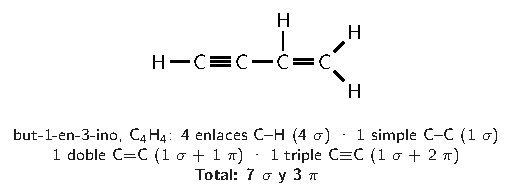
\includegraphics[max width=0.92\linewidth,max height=8.5cm]{qui/org_sigma_pi}
\end{center}
 
\begin{ojo}[{Error típico}] Contar el triple como 3 $\sigma$, o "olvidar" los C--H porque no se dibujan en la fórmula topológica. Los C--H también son enlaces $\sigma$.\end{ojo}
\subsection{Hibridación: sp³, sp² y sp}
Para formar sus enlaces, el carbono "mezcla" su orbital 2s con orbitales 2p y obtiene orbitales nuevos, iguales entre sí: los \textbf{orbitales híbridos}. Cuántos mezcla depende de cuántos enlaces $\pi$ tenga que formar.

 
\begin{center}
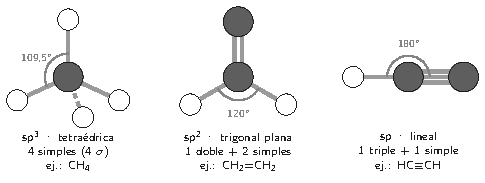
\includegraphics[max width=0.92\linewidth,max height=8.5cm]{qui/org_geometrias}
\end{center}
 
\begin{center}\small
\begin{tabularx}{\linewidth}{@{}>{\raggedright\arraybackslash\hsize=0.76\hsize}X>{\raggedright\arraybackslash\hsize=1.68\hsize}X>{\raggedright\arraybackslash\hsize=0.97\hsize}X>{\raggedright\arraybackslash\hsize=0.76\hsize}X>{\raggedright\arraybackslash\hsize=0.49\hsize}X>{\raggedright\arraybackslash\hsize=1.35\hsize}X@{}}
\toprule
\textbf{Hibridación} & \textbf{Enlaces del C} & \textbf{Átomos unidos al C} & \textbf{Geometría} & \textbf{Ángulo} & \textbf{Ejemplo} \\
\midrule
sp\textsuperscript{3} & 4 simples & 4 & tetraédrica & 109,5° & CH\textsubscript{4}, alcanos, C de un CH\textsubscript{3} \\
sp\textsuperscript{2} & 1 doble + 2 simples & 3 & trigonal plana & 120° & eteno, C=O, benceno \\
sp & 1 triple + 1 simple, o 2 dobles & 2 & lineal & 180° & etino, C\ensuremath{\equiv}N, C del CO\textsubscript{2} \\
\bottomrule
\end{tabularx}
\end{center}
 
\gatotip[\gatoatigrado]{\textbf{Regla rápida.} Mira solo al carbono que te preguntan: \textbf{solo simples \ensuremath{\rightarrow} sp³}; \textbf{un doble \ensuremath{\rightarrow} sp²}; \textbf{un triple o dos dobles \ensuremath{\rightarrow} sp}. También sirve contar los átomos unidos a él: 4 \ensuremath{\rightarrow} sp³, 3 \ensuremath{\rightarrow} sp², 2 \ensuremath{\rightarrow} sp.}
\subsection{Energía, longitud y ángulo de enlace}
Mientras más pares de electrones comparten dos carbonos, más \textbf{cerca} quedan sus núcleos y más \textbf{energía} cuesta separarlos.

 
\begin{center}\small
\begin{tabular}{@{}llll@{}}
\toprule
\textbf{Enlace} & \textbf{Hibridación} & \textbf{Longitud} & \textbf{Energía de enlace} \\
\midrule
C--C & sp\textsuperscript{3} & 154 pm (0,154 nm) & 347 kJ/mol \\
C=C & sp\textsuperscript{2} & 134 pm (0,134 nm) & 614 kJ/mol \\
C\ensuremath{\equiv}C & sp & 120 pm (0,120 nm) & 839 kJ/mol \\
\bottomrule
\end{tabular}
\end{center}
 

\textbf{Longitud de enlace}: distancia entre los núcleos. Disminuye: C--C > C=C > C\ensuremath{\equiv}C.\par \textbf{Energía de enlace}: energía necesaria para romperlo. Aumenta: C--C < C=C < C\ensuremath{\equiv}C.\par \textbf{Ángulo de enlace}: depende de la hibridación (109,5°, 120° o 180°).

  
\begin{ejemplo}[{Ejemplo resuelto}] ¿El doble enlace vale el doble que el simple? $2 \cdot 347 = 694$ kJ/mol, pero el C=C tiene 614. El enlace $\pi$ aporta solo $614 - 347 = 267$ kJ/mol: es \textbf{más débil} que el $\sigma$. Por eso alquenos y alquinos son más reactivos que los alcanos: el $\pi$ se rompe primero.\end{ejemplo}
 
\begin{ojo}[{Ojo con las unidades}] El DEMRE puede dar las longitudes en nm (0,154) o en pm (154). $1\ \text{nm} = 1000\ \text{pm}$. Para comparar, usa la misma unidad en todas.\end{ojo}
 
\begin{ojo}[{Error típico}] Creer que "más enlaces = más largo". Es al revés: el triple es el \textbf{más corto} y el \textbf{más fuerte}.\end{ojo}
\subsection{Ejemplo: hibridación y enlaces átomo por átomo}
El acrilonitrilo, CH\textsubscript{2}=CH--C\ensuremath{\equiv}N, se usa para fabricar fibras acrílicas. Analicemos cada carbono, numerando de izquierda a derecha.

 

\textbf{Paso 1. C1 (CH\textsubscript{2}=).} Tiene un doble enlace y dos H: 3 átomos unidos \ensuremath{\rightarrow} \textbf{sp²}, 120°.

 

\textbf{Paso 2. C2 (=CH--).} Un doble, un H y un simple: 3 átomos unidos \ensuremath{\rightarrow} \textbf{sp²}, 120°.

 

\textbf{Paso 3. C3 (--C\ensuremath{\equiv}N).} Un simple y un triple: 2 átomos unidos \ensuremath{\rightarrow} \textbf{sp}, 180°. Por eso C2, C3 y N están en línea recta.

 

\textbf{Paso 4. Enlaces.} Átomos: 3 C + 3 H + 1 N = 7, sin anillos \ensuremath{\rightarrow} $7 - 1 = 6$ enlaces $\sigma$. Enlaces $\pi$: 1 (del doble) + 2 (del triple) = 3.

 

\textbf{Comprobación:} contando uno por uno: 3 C--H + C1=C2 + C2--C3 + C3\ensuremath{\equiv}N = 6 enlaces, cada uno con 1 $\sigma$. \ding{52}

  
\begin{clave}[{Lo mismo con un grupo carbonilo}] En el ácido acético, CH\textsubscript{3}--COOH: el C del CH\textsubscript{3} es sp³ y el C del COOH es \textbf{sp²}, porque tiene un doble enlace C=O. Los dobles con O o N también cuentan.\end{clave}
 
\begin{ojo}[{Error típico}] Pensar que un C unido a un OH es sp³ "porque el OH es simple". Mira \textbf{todos} sus enlaces: el C del COOH tiene un C=O, así que es sp².\end{ojo}
\subsection{Lo clave del tema}
\begin{center}\small
\begin{tabularx}{\linewidth}{@{}>{\raggedright\arraybackslash\hsize=1.30\hsize}X>{\raggedright\arraybackslash\hsize=0.57\hsize}X>{\raggedright\arraybackslash\hsize=0.81\hsize}X>{\raggedright\arraybackslash\hsize=1.02\hsize}X>{\raggedright\arraybackslash\hsize=1.30\hsize}X@{}}
\toprule
\textbf{Enlaces del carbono} & \textbf{Hibridación} & \textbf{Geometría y ángulo} & \textbf{$\sigma$ y $\pi$ de ese enlace} & \textbf{Longitud / energía} \\
\midrule
4 simples & sp\textsuperscript{3} & tetraédrica, 109,5° & simple: 1 $\sigma$ & C--C: la más larga, la más débil \\
1 doble + 2 simples & sp\textsuperscript{2} & trigonal plana, 120° & doble: 1 $\sigma$ + 1 $\pi$ & C=C: intermedia \\
1 triple + 1 simple (o 2 dobles) & sp & lineal, 180° & triple: 1 $\sigma$ + 2 $\pi$ & C\ensuremath{\equiv}C: la más corta, la más fuerte \\
\bottomrule
\end{tabularx}
\end{center}
  
\begin{clave}[{Recuerda}] · El triple enlace tiene 1 $\sigma$ y 2 $\pi$.\par · Cada C--H es un enlace $\sigma$.\par · El C de un C=O es sp².\par · Más enlaces entre dos átomos: enlace más corto y más fuerte.\end{clave}
  
\begin{clave}[{Método PAES}] 1. Completa los H que faltan (4 enlaces por C). 2. Para hibridación, mira cada carbono por separado y cuenta sus átomos vecinos. 3. Para $\sigma$: un $\sigma$ por cada enlace (o átomos \ensuremath{-} 1, más 1 por anillo). Para $\pi$: 1 por doble, 2 por triple. 4. Revisa si te piden el total o solo los C--C.\end{clave}
\begin{elejemplo}{PAES Invierno 2027, adaptada}
La siguiente figura representa la molécula de etinilbenceno (fenilacetileno), usada en la síntesis de polímeros conductores.

Al respecto, ¿qué opción contiene el número correcto de enlaces de la molécula?
\begin{center}
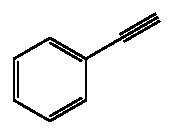
\includegraphics[max width=0.92\linewidth,max height=8.5cm]{qui/org_fenilacetileno}
\end{center}
{\centering\small\color{gris}Etinilbenceno (fórmula topológica)\par}
\alts{8 $\sigma$ (C--C), 5 $\pi$ (C--C) y 6 $\sigma$ (C--H)}{8 $\sigma$ (C--C), 2 $\pi$ (C--C) y 6 $\sigma$ (C--H)}{7 $\sigma$ (C--C), 5 $\pi$ (C--C) y 5 $\sigma$ (C--H)}{10 $\sigma$ (C--C), 5 $\pi$ (C--C) y 6 $\sigma$ (C--H)}
\solucion{\textbf{Paso 1. ¿Qué nos piden?} Tres conteos: enlaces $\sigma$ entre carbonos, enlaces $\pi$ entre carbonos y enlaces $\sigma$ C--H.

 

\textbf{Paso 2. Cuenta los carbonos.} El anillo tiene 6 vértices (6 C) y la cadena lateral tiene 2 C (el vértice unido al anillo y el extremo del triple). Total: 8 C, fórmula C\textsubscript{8}H\textsubscript{6}.

 

\textbf{Paso 3. Enlaces C--C y sus $\sigma$.} En el anillo hay 6 enlaces C--C; el anillo se une a la cadena con 1 enlace; y el triple es 1 enlace más. Son 8 enlaces C--C, y cada uno tiene exactamente 1 $\sigma$: \textbf{8 $\sigma$ (C--C)}.

 

\textbf{Paso 4. Enlaces $\pi$.} El anillo dibujado tiene 3 dobles (3 $\pi$) y el triple aporta 2 $\pi$: \textbf{5 $\pi$}.

 

\textbf{Paso 5. Enlaces C--H.} Completa a 4 enlaces cada C del anillo: el C unido a la cadena tiene 3 vecinos (2 del anillo y 1 de la cadena) y uno de esos enlaces es doble, así que ya suma 4 y no lleva H; los otros 5 C del anillo llevan 1 H cada uno. El C terminal del triple lleva 1 H (3 del triple + 1 H = 4). Total: \textbf{6 $\sigma$ (C--H)}.

 

\textbf{Respuesta:} 8 $\sigma$ (C--C), 5 $\pi$ (C--C) y 6 $\sigma$ (C--H).

 

\textbf{Comprobación:} la molécula tiene $8 + 6 = 14$ átomos y 1 anillo, así que debe tener $14 - 1 + 1 = 14$ enlaces $\sigma$ en total: $8 + 6 = 14$. \ding{52}

 

\textbf{¿Por qué no las otras?} "2 $\pi$" cuenta solo el triple y olvida los 3 dobles del anillo. "7 $\sigma$ y 5 C--H" olvida el enlace entre el anillo y la cadena, y el H del extremo del triple. "10 $\sigma$" cuenta el triple como 3 enlaces $\sigma$, pero un triple tiene 1 $\sigma$ y 2 $\pi$.

\textbf{\color{cienciaD}Para recordar.} Cada enlace (simple, doble o triple) aporta un solo sigma; los pi son las líneas extra: 1 por doble y 2 por triple.}{A}
\end{elejemplo}

%% =====================================================================
%% qui_representaciones
\section[Modelos de representación de moléculas]{Modelos de representación de moléculas}
\modcomun\ \ {\color{gris}\itshape Fórmula molecular, empírica, desarrollada, semidesarrollada, condensada y topológica, y los modelos de esferas y varillas y compacto: qué muestra cada una y cómo pasar de una a otra contando C e H.\par}
\subsection{Fórmula molecular y fórmula empírica}
La \textbf{fórmula molecular} dice qué átomos tiene una molécula y \textbf{cuántos exactamente}. El butano es C\textsubscript{4}H\textsubscript{10}: 4 C y 10 H.

 

La \textbf{fórmula empírica} da solo la \textbf{proporción mínima entera} entre los átomos. Se obtiene dividiendo todos los subíndices por su máximo común divisor (MCD).

 

\textbf{Paso 1.} Escribe la fórmula molecular: C\textsubscript{6}H\textsubscript{12}O\textsubscript{6} (glucosa).\par \textbf{Paso 2.} Busca el MCD de 6, 12 y 6: es 6.\par \textbf{Paso 3.} Divide: C\textsubscript{1}H\textsubscript{2}O\textsubscript{1} \ensuremath{\rightarrow} \textbf{CH\textsubscript{2}O}.

 
\begin{center}\small
\begin{tabular}{@{}lll@{}}
\toprule
\textbf{Compuesto} & \textbf{Molecular} & \textbf{Empírica} \\
\midrule
butano & C\textsubscript{4}H\textsubscript{10} & C\textsubscript{2}H\textsubscript{5} \\
benceno & C\textsubscript{6}H\textsubscript{6} & CH \\
etino & C\textsubscript{2}H\textsubscript{2} & CH \\
ácido etanoico & C\textsubscript{2}H\textsubscript{4}O\textsubscript{2} & CH\textsubscript{2}O \\
cloroformo & CHCl\textsubscript{3} & CHCl\textsubscript{3} \\
\bottomrule
\end{tabular}
\end{center}
  
\begin{clave}[{Ya es mínima}] Si el MCD es 1, la empírica es igual a la molecular. Le pasa al cloroformo (CHCl\textsubscript{3}), a la vanilina (C\textsubscript{8}H\textsubscript{8}O\textsubscript{3}) y al propano (C\textsubscript{3}H\textsubscript{8}).\end{clave}
 
\begin{ojo}[{Error típico}] Dividir solo algunos subíndices, o dividir aunque no den enteros. En C\textsubscript{8}H\textsubscript{8}O\textsubscript{3}, el 3 no se puede dividir por 8: la fórmula ya es empírica.\end{ojo}
 
\begin{ojo}[{Ojo}] Distintas sustancias pueden tener la misma empírica: el etino y el benceno son ambos CH. La empírica sola no identifica un compuesto.\end{ojo}
\subsection{Desarrollada, semidesarrollada, condensada y topológica}
Las fórmulas estructurales muestran, además, \textbf{cómo están unidos} los átomos. Mira las cuatro formas de escribir el butano:

 
\begin{center}
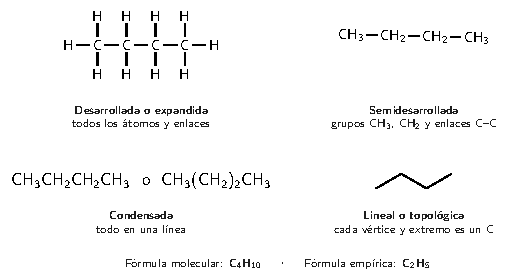
\includegraphics[max width=0.92\linewidth,max height=8.5cm]{qui/org_repr_butano}
\end{center}
  
\begin{itemize}
  \item \textbf{Desarrollada o expandida}: todos los átomos y todos los enlaces, uno por uno.
  \item \textbf{Semidesarrollada}: se agrupan los H con su carbono (CH\textsubscript{3}, CH\textsubscript{2}) y se dibujan los enlaces entre carbonos.
\end{itemize}
  
\begin{itemize}
  \item \textbf{Condensada}: todo en una línea, sin guiones; los grupos repetidos van entre paréntesis.
  \item \textbf{Lineal o topológica}: solo un zig-zag; cada vértice y cada extremo es un carbono.
\end{itemize}
\subsection{Cómo leer una fórmula topológica}
La fórmula topológica es la más usada en la PAES, porque es rápida de dibujar. Sus reglas:

 
\begin{itemize}
  \item Cada \textbf{vértice} y cada \textbf{extremo} de línea es un átomo de C.
  \item Los H unidos a carbono \textbf{no se dibujan}: cada C tiene los H que le faltan para llegar a 4 enlaces.
  \item Los otros átomos (O, N, Cl, S) \textbf{sí se escriben}, con sus H (OH, NH\textsubscript{2}).
  \item Una línea doble es un enlace doble; una triple, un triple.
\end{itemize}
 
\begin{center}
\includegraphics[max width=0.92\linewidth,max height=8.5cm]{qui/org_topo_prenol}
\end{center}
  
\begin{ejemplo}[{Ejemplo resuelto: contar C e H}] En la figura (3-metilbut-2-en-1-ol):\par \textbf{Paso 1. Carbonos.} 2 extremos arriba e izquierda + el vértice que los une + el vértice del doble + el vértice antes del OH = 5 C.\par \textbf{Paso 2. H de cada C} = 4 \ensuremath{-} (enlaces que ya tiene):\par · los dos CH\textsubscript{3} de los extremos: 3 + 3\par · el C con el doble y dos ramas: 4 \ensuremath{-} 4 = 0\par · el =CH--: 4 \ensuremath{-} 3 = 1\par · el CH\textsubscript{2} unido al OH: 4 \ensuremath{-} 2 = 2\par · el H del OH: 1\par \textbf{Paso 3.} Total: $3 + 3 + 0 + 1 + 2 + 1 = 10$ H. Fórmula: \textbf{C\textsubscript{5}H\textsubscript{10}O}.\end{ejemplo}
 
\begin{ojo}[{Errores típicos}] Olvidar los carbonos de los extremos, olvidar el H del OH, o poner H en un carbono que ya tiene 4 enlaces (por ejemplo, el que tiene un doble y dos ramas).\end{ojo}
\subsection{Modelos tridimensionales: esferas y varillas, y compacto}
\begin{center}
\includegraphics[max width=0.92\linewidth,max height=8.5cm]{qui/org_modelos}
\end{center}
  

\textbf{Modelo de esferas y varillas}: cada átomo es una esfera y cada enlace es una varilla. Muestra la \textbf{forma 3D}, los \textbf{ángulos de enlace} (109,5°, 120°, 180°) y cómo se ordenan los átomos en el espacio.

 

\textbf{Modelo compacto} (o de espacio lleno): las esferas se tocan y se superponen, a escala de su tamaño real. Muestra el \textbf{volumen} y la \textbf{forma externa} de la molécula, pero los enlaces y ángulos se ven poco.

  
\begin{clave}[{Colores habituales}] C: gris o negro · H: blanco · O: rojo · N: azul · Cl: verde.\end{clave}
 
\begin{ojo}[{Clave PAES}] Si dos formas de una molécula se diferencian solo en cómo se ordenan sus átomos \textbf{en el espacio}, ninguna fórmula escrita en el plano (molecular, empírica, condensada) las distingue: se necesita un modelo 3D, como el de esferas y varillas.\end{ojo}
\subsection{Comparar representaciones y moléculas}
\begin{center}\small
\begin{tabularx}{\linewidth}{@{}>{\raggedright\arraybackslash\hsize=1.29\hsize}X>{\raggedright\arraybackslash\hsize=1.29\hsize}X>{\raggedright\arraybackslash\hsize=0.67\hsize}X>{\raggedright\arraybackslash\hsize=0.76\hsize}X@{}}
\toprule
\textbf{Representación} & \textbf{¿Cuántos átomos de cada tipo?} & \textbf{¿Cómo se unen?} & \textbf{¿Forma 3D?} \\
\midrule
Empírica & solo la proporción & no & no \\
Molecular & sí & no & no \\
Condensada / semidesarrollada & sí & sí (por grupos) & no \\
Desarrollada / topológica & sí & sí & no (dibujo plano) \\
Esferas y varillas / compacto & sí & sí & sí \\
\bottomrule
\end{tabularx}
\end{center}
  
\begin{ejemplo}[{Ejemplo resuelto}] Etanol, CH\textsubscript{3}--CH\textsubscript{2}--OH, y metoximetano, CH\textsubscript{3}--O--CH\textsubscript{3}. \textbf{Paso 1.} Cuenta: los dos tienen 2 C, 6 H y 1 O: fórmula molecular C\textsubscript{2}H\textsubscript{6}O. \textbf{Paso 2.} Masa molar (H = 1, C = 12, O = 16): $2 \cdot 12 + 6 \cdot 1 + 16 = 46$ g/mol los dos. \textbf{Paso 3.} Pero la semidesarrollada muestra que son \textbf{distintos}: uno tiene O--H y el otro C--O--C. Son \textbf{isómeros}.\end{ejemplo}
  
\begin{ojo}[{Ojo con la masa molar}] Igual fórmula molecular implica igual masa molar. Pero igual masa molar \textbf{no} implica igual fórmula: el butan-2-ol (C\textsubscript{4}H\textsubscript{10}O) y el ácido propanoico (C\textsubscript{3}H\textsubscript{6}O\textsubscript{2}) pesan ambos 74 g/mol.\end{ojo}
\subsection{Lo clave del tema}
\begin{center}\small
\begin{tabularx}{\linewidth}{@{}>{\raggedright\arraybackslash\hsize=0.90\hsize}X>{\raggedright\arraybackslash\hsize=0.96\hsize}X>{\raggedright\arraybackslash\hsize=1.14\hsize}X@{}}
\toprule
\textbf{Representación} & \textbf{Butano} & \textbf{Lo que la distingue} \\
\midrule
Molecular & C\textsubscript{4}H\textsubscript{10} & número exacto de átomos \\
Empírica & C\textsubscript{2}H\textsubscript{5} & proporción mínima (divide por el MCD) \\
Desarrollada & todos los H y enlaces dibujados & todos los enlaces \\
Semidesarrollada & CH\textsubscript{3}--CH\textsubscript{2}--CH\textsubscript{2}--CH\textsubscript{3} & grupos CH\textsubscript{n} + enlaces C--C \\
Condensada & CH\textsubscript{3}(CH\textsubscript{2})\textsubscript{2}CH\textsubscript{3} & una línea, sin enlaces \\
Topológica & zig-zag de 4 vértices & vértices y extremos = C; H implícitos \\
Esferas y varillas / compacto & modelo 3D & ángulos / volumen \\
\bottomrule
\end{tabularx}
\end{center}
  
\begin{clave}[{Recuerda}] · En la fórmula topológica, cada extremo es un CH\textsubscript{3} (si no hay otro átomo escrito).\par · C\textsubscript{8}H\textsubscript{8}O\textsubscript{3} ya es empírica: el MCD de 8, 8 y 3 es 1.\par · Isómeros = misma fórmula molecular.\end{clave}
  
\begin{clave}[{Método PAES para contar}] 1. Marca cada vértice y extremo (C). 2. Para cada C: H = 4 \ensuremath{-} enlaces dibujados (doble cuenta 2, triple cuenta 3). 3. Suma los H de OH, NH\textsubscript{2}, CHO escritos. 4. Escribe C, H y luego los demás átomos. 5. Si piden la empírica, divide por el MCD.\end{clave}
\begin{elejemplo}{PAES Invierno 2026, adaptada}
Durante una clase de química orgánica, cuatro estudiantes analizan las estructuras de los compuestos X, Y y Z (masas atómicas: H = 1, C = 12, O = 16):

Luego, cada uno escribe en su cuaderno lo siguiente:

Estudiante 1: X e Y tienen la misma fórmula molecular.\par Estudiante 2: Z tiene más átomos de carbono que X.\par Estudiante 3: X y Z tienen la misma fórmula molecular, porque tienen la misma masa molar.\par Estudiante 4: Y tiene el doble de átomos de hidrógeno que Z.

¿Cuál de los estudiantes escribe una conclusión correcta?
\begin{center}
\includegraphics[max width=0.92\linewidth,max height=8.5cm]{qui/org_xyz}
\end{center}
\alts{El estudiante 1.}{El estudiante 2.}{El estudiante 3.}{El estudiante 4.}
\solucion{\textbf{Paso 1. ¿Qué nos piden?} La única afirmación correcta. Para eso necesitamos la fórmula molecular de X, Y y Z.

 

\textbf{Paso 2. Compuesto X.} Cuatro vértices/extremos: 4 C. H: extremo izquierdo CH\textsubscript{3} (3), vértice con OH: tiene 2 C y el O, le falta 1 H (1), siguiente vértice CH\textsubscript{2} (2), extremo CH\textsubscript{3} (3), más el H del OH (1). Total 10 H. \textbf{X = C\textsubscript{4}H\textsubscript{10}O} (butan-2-ol).

 

\textbf{Paso 3. Compuesto Y.} Dos C a cada lado del O: 4 C. Extremos CH\textsubscript{3} (3 + 3) y vértices junto al O, CH\textsubscript{2} (2 + 2). Total 10 H. \textbf{Y = C\textsubscript{4}H\textsubscript{10}O} (etoxietano).

 

\textbf{Paso 4. Compuesto Z.} 3 C: extremo CH\textsubscript{3} (3), vértice CH\textsubscript{2} (2) y el C del COOH (0 H sobre el C), más el H del OH (1). Total 6 H. \textbf{Z = C\textsubscript{3}H\textsubscript{6}O\textsubscript{2}} (ácido propanoico).

 

\textbf{Paso 5. Revisa cada estudiante.} 1: X e Y son ambos C\textsubscript{4}H\textsubscript{10}O. \ding{52} 2: Z tiene 3 C y X tiene 4. \ding{56} 3: X (C\textsubscript{4}H\textsubscript{10}O) y Z (C\textsubscript{3}H\textsubscript{6}O\textsubscript{2}) son fórmulas distintas. \ding{56} 4: Y tiene 10 H y Z tiene 6; el doble de 6 sería 12. \ding{56}

 

\textbf{Respuesta:} el estudiante 1.

 

\textbf{Comprobación:} masas molares: X = $4 \cdot 12 + 10 + 16 = 74$ g/mol; Z = $3 \cdot 12 + 6 + 2 \cdot 16 = 74$ g/mol. Tienen igual masa molar, pero distinta fórmula: por eso el estudiante 3 se equivoca, aunque su dato de masa sea cierto.

 

\textbf{¿Por qué no las otras?} El estudiante 2 no cuenta el carbono del extremo izquierdo de X o cuenta uno de más en Z. El estudiante 3 confunde "misma masa molar" con "misma fórmula". El estudiante 4 olvida que el doble de 6 es 12, no 10.

\textbf{\color{cienciaD}Para recordar.} Para comparar moléculas dibujadas, primero escribe la fórmula molecular de cada una: igual masa molar no significa igual fórmula.}{A}
\end{elejemplo}

%% =====================================================================
%% qui_hidrocarburos
\section[Hidrocarburos y nomenclatura IUPAC]{Hidrocarburos y nomenclatura IUPAC}
\modcomun\ \ {\color{gris}\itshape Alcanos, alquenos, alquinos, cíclicos y aromáticos: sus fórmulas generales, cómo encontrar la cadena principal, cómo numerarla y nombrar con ramificaciones, y qué son los isómeros.\par}
\subsection{Clasificación de los hidrocarburos}
Los \textbf{hidrocarburos} son compuestos formados \textbf{solo por C e H}. Son la base del petróleo, del gas natural y de los combustibles.

 
\begin{itemize}
  \item \textbf{Alifáticos} (cadena abierta, lineal o ramificada): 
\begin{itemize}
  \item \textbf{alcanos}: solo enlaces simples (\textbf{saturados}), sufijo \textbf{-ano};
  \item \textbf{alquenos}: al menos un C=C, sufijo \textbf{-eno};
  \item \textbf{alquinos}: al menos un C\ensuremath{\equiv}C, sufijo \textbf{-ino}.
\end{itemize}
  \item \textbf{Cíclicos}: la cadena se cierra en un anillo (prefijo \textbf{ciclo-}): ciclopropano, ciclohexano, ciclohexeno.
  \item \textbf{Aromáticos}: tienen el anillo del \textbf{benceno}.
\end{itemize}
 

Alquenos y alquinos son \textbf{insaturados}: tienen enlaces $\pi$ y dan reacciones de adición (por ejemplo, con H\textsubscript{2} o Br\textsubscript{2}).

  
\begin{center}
\includegraphics[max width=0.92\linewidth,max height=8.5cm]{qui/org_familias}
\end{center}
\subsection{Fórmulas generales y prefijos}
\begin{center}\small
\begin{tabular}{@{}lll@{}}
\toprule
\textbf{Familia} & \textbf{Fórmula general} & \textbf{Ejemplo} \\
\midrule
Alcano & C\textsubscript{n}H\textsubscript{2n+2} & propano C\textsubscript{3}H\textsubscript{8} \\
Alqueno (un doble) & C\textsubscript{n}H\textsubscript{2n} & propeno C\textsubscript{3}H\textsubscript{6} \\
Alquino (un triple) & C\textsubscript{n}H\textsubscript{2n\ensuremath{-}2} & propino C\textsubscript{3}H\textsubscript{4} \\
Cicloalcano & C\textsubscript{n}H\textsubscript{2n} & ciclopropano C\textsubscript{3}H\textsubscript{6} \\
Benceno & C\textsubscript{6}H\textsubscript{6} & --- \\
\bottomrule
\end{tabular}
\end{center}
 
\begin{clave}[{Regla de los 2 H}] Parte del alcano (C\textsubscript{n}H\textsubscript{2n+2}) y resta \textbf{2 H} por cada doble enlace o anillo, y \textbf{4 H} por cada triple. Ejemplo: C\textsubscript{6}H\textsubscript{10} = $14 - 4$: puede ser un hexino, un hexadieno o un ciclohexeno.\end{clave}
  
\begin{center}\small
\begin{tabular}{@{}llll@{}}
\toprule
\textbf{N.º de C} & \textbf{Prefijo} & \textbf{N.º de C} & \textbf{Prefijo} \\
\midrule
1 & met- & 6 & hex- \\
2 & et- & 7 & hept- \\
3 & prop- & 8 & oct- \\
4 & but- & 9 & non- \\
5 & pent- & 10 & dec- \\
\bottomrule
\end{tabular}
\end{center}
 
\begin{ojo}[{Ojo}] Un alqueno y un cicloalcano con los mismos C tienen la misma fórmula: el propeno y el ciclopropano son ambos C\textsubscript{3}H\textsubscript{6}.\end{ojo}
\subsection{Nombrar cadenas sin ramificar: la convención que usamos}
En este curso usamos las \textbf{recomendaciones IUPAC vigentes}, las mismas de las pruebas DEMRE: el número que indica la posición del doble o triple enlace (el \textbf{localizador}) va \textbf{justo antes del sufijo}.

 

\textbf{Paso 1.} Cuenta los C de la cadena que contiene el enlace múltiple: da el prefijo.\par \textbf{Paso 2.} Numera desde el extremo más cercano al enlace múltiple.\par \textbf{Paso 3.} Escribe prefijo + localizador + sufijo.

 
\begin{center}\small
\begin{tabular}{@{}ll@{}}
\toprule
\textbf{Estructura} & \textbf{Nombre} \\
\midrule
CH\textsubscript{2}=CH--CH\textsubscript{2}--CH\textsubscript{3} & but-1-eno \\
CH\textsubscript{3}--CH=CH--CH\textsubscript{3} & but-2-eno \\
CH\textsubscript{3}--C\ensuremath{\equiv}C--CH\textsubscript{2}--CH\textsubscript{3} & pent-2-ino \\
CH\textsubscript{2}=CH--CH=CH\textsubscript{2} & buta-1,3-dieno \\
\bottomrule
\end{tabular}
\end{center}
  
\begin{ojo}[{Nombres antiguos}] En libros más antiguos verás "2-buteno", "1-butino" o "2-pentino": son los \textbf{mismos compuestos} que but-2-eno, but-1-ino y pent-2-ino. Solo cambia dónde se escribe el número. En la PAES aparece la forma nueva ("penta-2-ino", "butan-2-ona").\end{ojo}
 
\begin{clave}[{Detalles de escritura}] Con dos dobles se agrega una "a" al prefijo: \textbf{buta}-1,3-dieno. Si hay doble y triple, el "-eno" va antes: pent-1-en-3-ino. Con 1 o 2 carbonos no hace falta localizador: eteno, etino, propeno.\end{clave}
 
\begin{clave}[{Grupos alquilo (ramificaciones)}] --CH\textsubscript{3} metil · --CH\textsubscript{2}CH\textsubscript{3} etil · --CH\textsubscript{2}CH\textsubscript{2}CH\textsubscript{3} propil · --CH(CH\textsubscript{3})\textsubscript{2} isopropil.\end{clave}
\subsection{Nombrar con ramificaciones, paso a paso}
\begin{center}
\includegraphics[max width=0.92\linewidth,max height=8.5cm]{qui/org_nom_ejemplo}
\end{center}
  

\textbf{Paso 1. Cadena principal.} La más larga (y, si hay dobles o triples, la que los contiene). Aquí: 6 C \ensuremath{\rightarrow} \textbf{hexano}. Ojo: la cadena más larga puede doblar por una ramificación; no tiene que ser la horizontal.

 

\textbf{Paso 2. Numera} desde el extremo que dé los números más bajos: primero al enlace múltiple; si no hay, a las ramificaciones. Desde la izquierda: 2 y 4. Desde la derecha: 3 y 5. Gana la izquierda.

 

\textbf{Paso 3. Nombra las ramificaciones}: metil en C2, etil en C4.

 

\textbf{Paso 4. Ordena alfabéticamente} (etil antes que metil) y escribe: \textbf{4-etil-2-metilhexano}.

  
\begin{clave}[{Más reglas}] · Ramificaciones repetidas: di-, tri-, tetra-: 2,3-dimetilbutano. Estos prefijos no cuentan para el orden alfabético.\par · Números con comas entre sí y guion entre número y letra: 2,2-dimetilpropano.\par · Si dos cadenas igual de largas compiten, se elige la que tiene más ramificaciones.\end{clave}
 
\begin{ejemplo}[{Ejemplo con doble enlace}] CH\textsubscript{2}=C(CH\textsubscript{3})--CH\textsubscript{2}--CH\textsubscript{3}: cadena de 4 C con el doble; se numera desde el doble (C1). Metil en C2: \textbf{2-metilbut-1-eno}.\end{ejemplo}
\subsection{Hidrocarburos cíclicos y aromáticos}
\textbf{Cicloalcanos}: anillos de C con solo enlaces simples. Se nombran con \textbf{ciclo-} + el nombre del alcano: ciclopropano, ciclopentano, ciclohexano (C\textsubscript{6}H\textsubscript{12}). Con una ramificación: metilciclohexano.

 

\textbf{Aromáticos}: contienen el \textbf{benceno}, C\textsubscript{6}H\textsubscript{6}. Se dibuja con tres dobles alternados o con un círculo dentro del hexágono: sus electrones $\pi$ están \textbf{deslocalizados} en todo el anillo. Por eso el benceno es muy estable y, a diferencia de los alquenos, da reacciones de \textbf{sustitución} y no de adición.

 

Los 6 C del benceno son sp², el anillo es plano y sus ángulos miden 120°.

  
\begin{center}\small
\begin{tabularx}{\linewidth}{@{}>{\raggedright\arraybackslash\hsize=0.97\hsize}X>{\raggedright\arraybackslash\hsize=0.42\hsize}X>{\raggedright\arraybackslash\hsize=1.61\hsize}X@{}}
\toprule
\textbf{Aromático} & \textbf{Fórmula} & \textbf{Uso} \\
\midrule
benceno & C\textsubscript{6}H\textsubscript{6} & materia prima industrial (tóxico) \\
tolueno (metilbenceno) & C\textsubscript{7}H\textsubscript{8} & solvente de pinturas \\
estireno (vinilbenceno) & C\textsubscript{8}H\textsubscript{8} & fabricación de plumavit (poliestireno) \\
naftaleno & C\textsubscript{10}H\textsubscript{8} & antiguas bolitas de naftalina \\
\bottomrule
\end{tabularx}
\end{center}
 
\begin{ojo}[{Error típico}] Contar 2 H en cada C del benceno, como si fuera ciclohexano. En el benceno cada C tiene 1 H (o 0 si lleva un sustituyente).\end{ojo}
\subsection{Isómeros y temperatura de ebullición}
Los \textbf{isómeros} tienen la \textbf{misma fórmula molecular} pero \textbf{distinta estructura}, y por eso distintas propiedades.

 
\begin{itemize}
  \item \textbf{De cadena}: cambia el esqueleto. Butano y metilpropano (C\textsubscript{4}H\textsubscript{10}).
  \item \textbf{De posición}: cambia la ubicación del doble enlace o del grupo. But-1-eno y but-2-eno.
  \item \textbf{De función}: cambia el tipo de compuesto. Etanol y metoximetano (C\textsubscript{2}H\textsubscript{6}O); hex-1-eno y ciclohexano (C\textsubscript{6}H\textsubscript{12}).
\end{itemize}
 
\begin{clave}[{Dos tendencias que pregunta la PAES}] 1. En una serie de alcanos lineales, \textbf{a más carbonos, mayor temperatura de ebullición} (más superficie de contacto entre moléculas).\par 2. Entre isómeros, \textbf{a más ramificación, menor temperatura de ebullición} (la molécula es más compacta y se atrae menos con sus vecinas).\end{clave}
  
\begin{center}
\includegraphics[max width=0.92\linewidth,max height=8.5cm]{qui/org_isomeros_c5}
\end{center}
 
\begin{ojo}[{Ojo}] "3-metilbutano" no existe como nombre: numerado bien, es el 2-metilbutano. Y "1-metilbutano" es en realidad el pentano. Antes de contar isómeros, nombra cada uno para no repetir.\end{ojo}
\subsection{Lo clave del tema}
\begin{center}\small
\begin{tabularx}{\linewidth}{@{}>{\raggedright\arraybackslash\hsize=0.95\hsize}X>{\raggedright\arraybackslash\hsize=1.08\hsize}X>{\raggedright\arraybackslash\hsize=0.95\hsize}X>{\raggedright\arraybackslash\hsize=0.95\hsize}X>{\raggedright\arraybackslash\hsize=1.08\hsize}X@{}}
\toprule
\textbf{Familia} & \textbf{Enlace clave} & \textbf{Fórmula} & \textbf{Sufijo} & \textbf{Ejemplo} \\
\midrule
Alcano & solo simples & C\textsubscript{n}H\textsubscript{2n+2} & -ano & 2-metilbutano \\
Alqueno & C=C & C\textsubscript{n}H\textsubscript{2n} & -eno & but-2-eno \\
Alquino & C\ensuremath{\equiv}C & C\textsubscript{n}H\textsubscript{2n\ensuremath{-}2} & -ino & pent-2-ino \\
Cicloalcano & anillo, simples & C\textsubscript{n}H\textsubscript{2n} & ciclo-\dots{}-ano & ciclohexano \\
Aromático & anillo bencénico & C\textsubscript{6}H\textsubscript{6} (benceno) & -benceno & metilbenceno \\
\bottomrule
\end{tabularx}
\end{center}
  
\begin{clave}[{Recuerda}] · La cadena principal es la más larga, aunque se doble.\par · Los sustituyentes van en orden alfabético: 4-etil-2-metilhexano.\par · El doble enlace lleva el número más bajo: pent-2-eno.\par · Isómeros = misma fórmula molecular.\end{clave}
  
\begin{clave}[{Método PAES para nombrar}] 1. Busca la cadena más larga que contenga el doble o triple. 2. Numera para que el enlace múltiple (o, si no hay, las ramas) tenga el número más bajo. 3. Identifica ramas y su posición. 4. Escribe en orden alfabético: localizador-rama + prefijo + localizador + sufijo. 5. Revisa: ¿el total de C del nombre coincide con el dibujo?\end{clave}
\begin{elejemplo}{PAES Invierno 2027, adaptada}
Respecto de la siguiente estructura de un hidrocarburo:

¿Cuál es su nombre correcto, según la IUPAC?
\begin{center}
\includegraphics[max width=0.92\linewidth,max height=8.5cm]{qui/org_ej_nombre}
\end{center}
\alts{3,6-dimetilhept-4-eno}{2,5-dimetilheptano}{5-etil-2-metilhex-3-eno}{2,5-dimetilhept-3-eno}
\solucion{\textbf{Paso 1. ¿Qué nos piden?} El nombre IUPAC: cadena principal, numeración, ramificaciones y sufijo.

 

\textbf{Paso 2. Tipo de compuesto.} Solo C e H y una línea doble: es un \textbf{alqueno} (sufijo -eno).

 

\textbf{Paso 3. Cadena principal.} Busca la cadena más larga que contenga el doble enlace. Partiendo del extremo inferior izquierdo: 1 C, sube al vértice ramificado, baja, doble, sube, baja al otro vértice ramificado, y sigue por la derecha 2 C más. Son \textbf{7 C}: hept-. Las dos líneas que salen hacia arriba y hacia abajo de los vértices ramificados son metilos.

 

\textbf{Paso 4. Numeración.} Desde la izquierda, el doble enlace queda entre C3 y C4 \ensuremath{\rightarrow} localizador 3. Desde la derecha quedaría en 4. Gana la izquierda: \textbf{hept-3-eno}.

 

\textbf{Paso 5. Ramificaciones.} Con esa numeración, los metilos están en C2 y C5: \textbf{2,5-dimetil}.

 

\textbf{Respuesta:} 2,5-dimetilhept-3-eno.

 

\textbf{Comprobación:} el nombre indica $7 + 2 = 9$ C y el dibujo tiene 9 vértices y extremos. Fórmula: C\textsubscript{9}H\textsubscript{18} = C\textsubscript{n}H\textsubscript{2n}, como corresponde a un alqueno. \ding{52}

 

\textbf{¿Por qué no las otras?} "3,6-dimetilhept-4-eno" numera desde la derecha y le da al doble un número mayor (4 en vez de 3). "2,5-dimetilheptano" ignora el doble enlace (sería un alcano, C\textsubscript{9}H\textsubscript{20}). "5-etil-2-metilhex-3-eno" elige una cadena de 6 C cuando hay una de 7, y además deja una rama etilo que debería ser parte de la cadena.

\textbf{\color{cienciaD}Para recordar.} Cadena más larga con el doble enlace, numerada para que el doble tenga el número más bajo; luego las ramas en orden alfabético.}{D}
\end{elejemplo}

%% =====================================================================
%% qui_funcionales
\section[Grupos funcionales]{Grupos funcionales}
\modcomun\ \ {\color{gris}\itshape Haluros, alcoholes, fenoles, éteres, sulfuros, aldehídos, cetonas, ácidos carboxílicos, ésteres, anhídridos, amidas, aminas y nitrilos: cómo se escriben, cómo se nombran, cómo reconocerlos en fármacos y aromas, y para qué se usan.\par}
\subsection{¿Qué es un grupo funcional?}
Un \textbf{grupo funcional} es un átomo o grupo de átomos (casi siempre con O, N, S o un halógeno) que le da a la molécula sus propiedades químicas. Moléculas con el mismo grupo funcional se comportan de forma parecida.

 

Se escribe \textbf{R} para el resto de la molécula (la parte de C e H). Así, R--OH es "cualquier alcohol": CH\textsubscript{3}--OH, CH\textsubscript{3}--CH\textsubscript{2}--OH, etc.

 

Cuando una molécula tiene varios grupos, el de \textbf{mayor prioridad} da el sufijo del nombre y los demás se nombran como prefijos:

 
\begin{center}
\textbf{ácido carboxílico > anhídrido > éster > amida > nitrilo > aldehído > cetona > alcohol > amina > éter > haluro}
\end{center}
  
\begin{ejemplo}[{Ejemplo}] HO--CH\textsubscript{2}--CH\textsubscript{2}--CH\textsubscript{2}--COOH tiene un alcohol y un ácido. Manda el ácido: la cadena se numera desde el COOH (C1) y el OH queda en C4 como prefijo "hidroxi": \textbf{ácido 4-hidroxibutanoico}.\end{ejemplo}
 
\begin{ojo}[{Nombres comunes}] El temario acepta nombres IUPAC o comunes. Conviene saber los dos para los compuestos famosos: acetona = propanona, ácido acético = ácido etanoico, formaldehído = metanal, cloroformo = triclorometano.\end{ojo}
\subsection{Oxígeno con enlaces simples: alcoholes, fenoles y éteres}
\begin{center}
\includegraphics[max width=0.92\linewidth,max height=8.5cm]{qui/org_grupos_o}
\end{center}
  

\textbf{Alcohol, R--OH.} Sufijo \textbf{-ol}, con localizador: propan-2-ol. Ejemplos: metanol (tóxico), etanol (bebidas, alcohol gel, combustible), propan-2-ol (alcohol isopropílico, desinfectante), glicerol (cosméticos). Según el C que lleva el OH, son primarios (el C tiene 1 C vecino), secundarios (2) o terciarios (3). Forman \textbf{puentes de hidrógeno}: temperaturas de ebullición altas y los pequeños son solubles en agua.

 

\textbf{Fenol, OH unido a un anillo bencénico.} El fenol, C\textsubscript{6}H\textsubscript{5}OH, es desinfectante; los fenoles son antioxidantes y están en el timol del tomillo y en la vanilina. Son más ácidos que los alcoholes.

  

\textbf{Éter, R--O--R'.} El O está \textbf{entre dos carbonos}. IUPAC: el grupo pequeño con O se nombra "alcoxi": CH\textsubscript{3}--O--CH\textsubscript{2}--CH\textsubscript{3} es \textbf{metoxietano} (común: etil metil éter). El etoxietano (dietil éter) fue un anestésico y hoy es solvente. No forman puentes de hidrógeno entre sí: hierven a menor temperatura que el alcohol isómero.

 
\begin{ojo}[{Alcohol o fenol}] Si el OH está en un C del anillo bencénico, es fenol; si está en un C con solo enlaces simples, es alcohol.\end{ojo}
\subsection{El grupo carbonilo: aldehídos y cetonas}
El \textbf{carbonilo} es un C=O. Su posición define la familia:

 

\textbf{Aldehído, R--CHO.} El C=O está en un \textbf{extremo} de la cadena: el C lleva un H. Sufijo \textbf{-al}, sin número (el C del CHO siempre es C1): metanal, etanal, butanal. Ejemplos: metanal o formaldehído (la formalina conserva tejidos), benzaldehído (aroma de almendras), cinamaldehído (canela), vanilina (vainilla).

 

\textbf{Cetona, R--CO--R'.} El C=O está \textbf{entre dos carbonos}. Sufijo \textbf{-ona}, con localizador: pentan-2-ona, pentan-3-ona. La propanona (acetona) es el solvente del quitaesmalte; la butan-2-ona se usa en pinturas.

  
\begin{ejemplo}[{Ejemplo resuelto}] CH\textsubscript{3}--CH\textsubscript{2}--CH(CH\textsubscript{3})--CH\textsubscript{2}--CHO. \textbf{Paso 1.} Cadena más larga con el CHO: 5 C \ensuremath{\rightarrow} pentanal. \textbf{Paso 2.} El CHO es C1, así que el metilo queda en C3. \textbf{Nombre:} 3-metilpentanal. \textbf{Fórmula:} C\textsubscript{6}H\textsubscript{12}O.\end{ejemplo}
 
\begin{ojo}[{Error típico}] Llamar cetona a todo C=O. Mira los vecinos del carbono del C=O: si uno es H, es aldehído; si son dos C, es cetona; si uno es O o N, es ácido, éster o amida (siguiente sección).\end{ojo}
 
\begin{clave}[{Oxidación}] Alcohol primario \ensuremath{\rightarrow} aldehído \ensuremath{\rightarrow} ácido carboxílico. Alcohol secundario \ensuremath{\rightarrow} cetona.\end{clave}
\subsection{Ácidos carboxílicos y sus derivados: ésteres, anhídridos y amidas}
\begin{center}
\includegraphics[max width=0.92\linewidth,max height=8.5cm]{qui/org_grupos_co}
\end{center}
  

\textbf{Ácido carboxílico, R--COOH.} "ácido \dots{}-oico": ácido metanoico (fórmico, de las hormigas), ácido etanoico (acético, del vinagre), ácido butanoico (mantequilla rancia). Son ácidos débiles y forman puentes de hidrógeno.

 

\textbf{Éster, R--COO--R'.} Se forma por \textbf{esterificación}: ácido + alcohol \ensuremath{\rightarrow} éster + agua. Nombre: la parte del ácido termina en \textbf{-ato} y la del alcohol en \textbf{-ilo}: CH\textsubscript{3}--COO--CH\textsubscript{2}--CH\textsubscript{3} es \textbf{etanoato de etilo} (acetato de etilo). Dan los \textbf{aromas frutales}: etanoato de 3-metilbutilo (plátano), butanoato de etilo (piña). Las grasas y aceites son ésteres.

  

\textbf{Anhídrido, R--CO--O--CO--R.} Dos grupos acilo unidos por un O (como dos ácidos que perdieron una molécula de agua). El anhídrido etanoico (acético) se usa para fabricar la aspirina.

 

\textbf{Amida, R--CO--NH\textsubscript{2}.} Sufijo \textbf{-amida}: etanamida. La urea es una amida; el \textbf{enlace peptídico} que une los aminoácidos en las proteínas es una amida, igual que el nailon y el paracetamol.

 
\begin{ojo}[{Éster o éter}] Los dos tienen C--O--C, pero el éster tiene además un C=O pegado a ese O. Sin C=O, es éter.\end{ojo}
\subsection{Nitrógeno, azufre y halógenos: aminas, nitrilos, sulfuros y haluros}
\begin{center}
\includegraphics[max width=0.92\linewidth,max height=8.5cm]{qui/org_grupos_nsx}
\end{center}
  

\textbf{Amina, R--NH\textsubscript{2}} (también R\textsubscript{2}NH y R\textsubscript{3}N). Sufijo \textbf{-amina}: metanamina (metilamina). Son \textbf{básicas} y las pequeñas huelen a pescado. Están en los aminoácidos, la adrenalina, la anilina (colorantes) y alcaloides como la cafeína y la nicotina.

 

\textbf{Nitrilo, R--C\ensuremath{\equiv}N.} Sufijo \textbf{-nitrilo}, contando el C del CN: CH\textsubscript{3}--CN es etanonitrilo (acetonitrilo, un solvente). El propenonitrilo (acrilonitrilo) se usa para fibras acrílicas.

  

\textbf{Sulfuro (tioéter), R--S--R'.} Como un éter, pero con S: CH\textsubscript{3}--S--CH\textsubscript{3} es el sulfuro de dimetilo (olor a mar y a repollo cocido). El sulfuro de dialilo da parte del olor del ajo. No confundir con los tioles (R--SH), que se agregan al gas para detectar fugas.

 

\textbf{Haluro de alquilo, R--X} (X = F, Cl, Br, I). Se nombran con prefijos: clorometano, 2-bromopropano. El triclorometano (cloroformo) fue anestésico y hoy es solvente; los CFC dañan la capa de ozono; el PVC y el teflón son polímeros halogenados.
\subsection{Reconocer grupos en moléculas reales}
\begin{center}
\includegraphics[max width=0.92\linewidth,max height=8.5cm]{qui/org_reales}
\end{center}
  

En la PAES aparecen fármacos, aromas e insecticidas dibujados en fórmula topológica. Para reconocer sus grupos, mira cada heteroátomo (O, N, S, halógeno) y a sus \textbf{vecinos}:

 
\begin{center}\small
\begin{tabular}{@{}ll@{}}
\toprule
\textbf{Lo que ves} & \textbf{Grupo} \\
\midrule
OH en C con solo simples & alcohol \\
OH en el anillo bencénico & fenol \\
C--O--C, sin C=O al lado & éter \\
C=O en un extremo (con H) & aldehído \\
C=O entre dos C & cetona \\
C=O con OH en el mismo C & ácido carboxílico \\
C=O con O--C en el mismo C & éster \\
C=O con N en el mismo C & amida \\
N con solo enlaces simples a C o H & amina \\
C\ensuremath{\equiv}N & nitrilo \\
\bottomrule
\end{tabular}
\end{center}
  
\begin{ejemplo}[{Ejemplo resuelto: paracetamol}] HO--C\textsubscript{6}H\textsubscript{4}--NH--CO--CH\textsubscript{3}. \textbf{Paso 1.} El OH está sobre el anillo: \textbf{fenol}. \textbf{Paso 2.} El N está unido a un C que tiene un C=O: no es amina, es \textbf{amida}. \textbf{Paso 3.} No hay ácido ni éster: el único C=O es parte de la amida.\end{ejemplo}
 
\begin{ojo}[{Error típico}] Mirar un átomo solo. Un O puede ser alcohol, éter, cetona, éster o ácido según sus vecinos, y un N puede ser amina o amida. Revisa siempre el carbono de al lado.\end{ojo}
\subsection{Lo clave del tema}
\begin{center}\small
\begin{tabularx}{\linewidth}{@{}>{\raggedright\arraybackslash\hsize=0.72\hsize}X>{\raggedright\arraybackslash\hsize=0.60\hsize}X>{\raggedright\arraybackslash\hsize=1.15\hsize}X>{\raggedright\arraybackslash\hsize=1.53\hsize}X@{}}
\toprule
\textbf{Grupo} & \textbf{Fórmula} & \textbf{Nombre (ejemplo)} & \textbf{Uso o característica} \\
\midrule
Haluro & R--X & triclorometano (cloroformo) & solventes, CFC, PVC \\
Alcohol & R--OH & etanol & bebidas, desinfectante; puentes de H \\
Fenol & Ar--OH & fenol & desinfectante, antioxidante \\
Éter & R--O--R' & etoxietano (dietil éter) & anestésico antiguo, solvente \\
Sulfuro & R--S--R' & sulfuro de dimetilo & olores (ajo, mar) \\
Aldehído & R--CHO & metanal (formaldehído) & conservante (formalina), aromas \\
Cetona & R--CO--R' & propanona (acetona) & solvente, quitaesmalte \\
Ácido carboxílico & R--COOH & ácido etanoico (acético) & vinagre; ácido débil \\
Éster & R--COO--R' & etanoato de etilo & aromas frutales, grasas \\
Anhídrido & R--CO--O--CO--R & anhídrido etanoico & síntesis de aspirina \\
Amida & R--CO--NH\textsubscript{2} & etanamida & proteínas, nailon, paracetamol \\
Amina & R--NH\textsubscript{2} & metanamina (metilamina) & básicas, olor a pescado, alcaloides \\
Nitrilo & R--C\ensuremath{\equiv}N & etanonitrilo (acetonitrilo) & solventes, fibras acrílicas \\
\bottomrule
\end{tabularx}
\end{center}
  
\begin{clave}[{Recuerda}] · En un C=O mira los vecinos: H (aldehído), 2 C (cetona), OH (ácido), O--C (éster), N (amida).\par · N--C=O es una amida.\par · Etanoato de propilo y propanoato de etilo son distintos: "-ato" es la parte del ácido (con el C=O) y "-ilo" la del alcohol.\end{clave}
  
\begin{clave}[{Método PAES}] 1. Encierra cada heteroátomo. 2. Mira sus vecinos y usa la tabla de la sección anterior. 3. Si te piden el nombre, busca el grupo de mayor prioridad: da el sufijo y fija la numeración (C1 en el CHO o el COOH). 4. Si te piden un uso, asocia: éster--aroma, amida--proteínas, cetona--acetona, ácido--vinagre, amina--olor a pescado.\end{clave}
\begin{elejemplo}{PAES Regular 2026, adaptada}
El ácido acetilsalicílico (aspirina) es uno de los analgésicos más usados del mundo. Su estructura es la siguiente:

¿Cuáles grupos funcionales están presentes en esta molécula, además del anillo aromático?
\begin{center}
\includegraphics[max width=0.92\linewidth,max height=8.5cm]{qui/org_aspirina}
\end{center}
\alts{Cetona y éter}{Ácido carboxílico y éster}{Aldehído y alcohol}{Ácido carboxílico y cetona}
\solucion{\textbf{Paso 1. ¿Qué nos piden?} Nombrar los grupos funcionales que se ven en la estructura.

 

\textbf{Paso 2. Encierra los heteroátomos.} Hay 4 O, en dos grupos: uno a la derecha (C=O y OH) y otro arriba a la izquierda (un O unido al anillo y un C=O).

 

\textbf{Paso 3. Grupo de la derecha.} Un carbono tiene un C=O y un OH a la vez: es un \textbf{ácido carboxílico} (--COOH).

 

\textbf{Paso 4. Grupo de arriba.} El O unido al anillo está unido, del otro lado, a un C que tiene un C=O (y un CH\textsubscript{3}). Un O entre dos C, con C=O al lado: es un \textbf{éster} (--O--CO--CH\textsubscript{3}). No es éter, porque hay un C=O pegado; no es cetona, porque el C del C=O está unido a un O.

 

\textbf{Respuesta:} ácido carboxílico y éster.

 

\textbf{Comprobación:} la aspirina se fabrica haciendo reaccionar el ácido salicílico (que tiene un fenol) con anhídrido etanoico: el OH del fenol se convierte en el éster. Su fórmula es C\textsubscript{9}H\textsubscript{8}O\textsubscript{4}: los 4 O son los 2 del ácido y los 2 del éster. \ding{52}

 

\textbf{¿Por qué no las otras?} "Cetona y éter" mira el C=O y el C--O--C por separado, sin notar que están unidos: juntos son un éster. "Aldehído y alcohol" confunde el COOH con un CHO más un OH. "Ácido carboxílico y cetona" acierta el ácido, pero el otro C=O no está entre dos C: tiene un O al lado.

\textbf{\color{cienciaD}Para recordar.} Antes de nombrar un C=O o un O, mira a sus vecinos: juntos pueden formar un grupo distinto.}{B}
\end{elejemplo}

\chapter{Reacciones químicas y estequiometría}
%% =====================================================================
%% qui_leyes
\section[Leyes ponderales y balance de ecuaciones]{Leyes ponderales y balance de ecuaciones}
\modcomun\ \ {\color{gris}\itshape Las partes de una ecuación química, la conservación de la masa (Lavoisier), las proporciones definidas (Proust) y múltiples (Dalton), y cómo balancear una ecuación por tanteo.\par}
\subsection{Las partes de una ecuación química}
Una \textbf{reacción química} es un proceso en el que unas sustancias se transforman en otras distintas. Se escribe con una \textbf{ecuación química}:

 
\begin{center}
CH\textsubscript{4} (g) + 2 O\textsubscript{2} (g) \ensuremath{\rightarrow} CO\textsubscript{2} (g) + 2 H\textsubscript{2}O (l)
\end{center}
 

Se lee: «un metano gaseoso reacciona con dos oxígenos gaseosos y forma un dióxido de carbono gaseoso y dos aguas líquidas».

 
\begin{center}\small
\begin{tabularx}{\linewidth}{@{}>{\raggedright\arraybackslash\hsize=0.63\hsize}X>{\raggedright\arraybackslash\hsize=1.79\hsize}X>{\raggedright\arraybackslash\hsize=0.58\hsize}X@{}}
\toprule
\textbf{Parte} & \textbf{Qué es} & \textbf{En el ejemplo} \\
\midrule
Reactantes & lo que hay al comienzo, a la izquierda & CH\textsubscript{4} y O\textsubscript{2} \\
Productos & lo que se forma, a la derecha & CO\textsubscript{2} y H\textsubscript{2}O \\
Flecha & «reacciona y forma» & \ensuremath{\rightarrow} \\
Coeficiente & número \textbf{delante} de la fórmula: cuántas moléculas (o mol) & el 2 de 2 O\textsubscript{2} \\
Subíndice & número \textbf{pequeño abajo}: cuántos átomos hay en una molécula & el 4 de CH\textsubscript{4} \\
Estado & (s) sólido, (l) líquido, (g) gas, (ac) acuoso, disuelto en agua & (g), (l) \\
\bottomrule
\end{tabularx}
\end{center}
  
\begin{clave}[{Coeficiente por subíndice}] Para contar átomos, multiplica el coeficiente por el subíndice. En 2 H\textsubscript{2}O hay 2 moléculas de agua: $2\cdot 2 = 4$ átomos de H y $2\cdot 1 = 2$ átomos de O.\end{clave}
 
\begin{clave}[{Con paréntesis}] En 3 Ca(OH)\textsubscript{2} el 2 multiplica a todo el paréntesis: por fórmula hay 1 Ca, 2 O y 2 H. Con el coeficiente: 3 Ca, 6 O y 6 H.\end{clave}
 
\begin{ojo}[{Error típico}] Creer que el subíndice y el coeficiente significan lo mismo. 2 O (dos átomos de oxígeno sueltos) no es lo mismo que O\textsubscript{2} (una molécula de oxígeno), ni que 2 O\textsubscript{2} (dos moléculas, cuatro átomos).\end{ojo}
\subsection{Ley de conservación de la masa (Lavoisier)}
Antoine Lavoisier (siglo XVIII) masó con cuidado los reactantes y los productos de muchas reacciones hechas en recipientes cerrados y llegó a esta ley:

 
\begin{clave}[{Ley de Lavoisier}] En una reacción química, la masa total de los reactantes es igual a la masa total de los productos. La materia no se crea ni se destruye: se transforma.\end{clave}
 

\textbf{¿Por qué se cumple?} Mira el diagrama de partículas de 2 H\textsubscript{2} + O\textsubscript{2} \ensuremath{\rightarrow} 2 H\textsubscript{2}O. Los átomos solo se \textbf{reordenan}: se rompen unos enlaces y se forman otros, pero antes y después hay los mismos átomos (8 de H y 4 de O). Si los átomos son los mismos, la masa también.

 
\begin{center}
\includegraphics[max width=0.92\linewidth,max height=8.5cm]{qui/reac_particulas}
\end{center}
  
\begin{ejemplo}[{Ejemplo resuelto}] En un recipiente cerrado reaccionan completamente 12 g de magnesio con 8 g de oxígeno y se forma óxido de magnesio. ¿Qué masa de óxido se forma?\par \textbf{Paso 1.} Todo reaccionó: la masa de los reactantes es $12 + 8 = 20$ g.\par \textbf{Paso 2.} Por Lavoisier, la masa del producto es la misma: \textbf{20 g} de óxido de magnesio.\end{ejemplo}
 
\begin{clave}[{Si algo sobra}] Si en un recipiente cerrado pones 12 g de Mg y 10 g de O\textsubscript{2}, y se forman 20 g de óxido, la masa total sigue siendo $12 + 10 = 22$ g: son 20 g de óxido más $22 - 20 = 2$ g de oxígeno que \textbf{sobró} sin reaccionar.\end{clave}
 
\begin{ojo}[{Ojo}] Se conserva la \textbf{masa} y se conservan los \textbf{átomos}, pero no necesariamente el número de moléculas: en el diagrama hay 6 moléculas antes y 4 después.\end{ojo}
\subsection{Sistema abierto y sistema cerrado}
Cuando mezclas vinagre con bicarbonato se forma un gas, CO\textsubscript{2}. Si haces la reacción sobre una balanza, el resultado depende del recipiente:

 
\begin{center}
\includegraphics[max width=0.92\linewidth,max height=8.5cm]{qui/reac_balanza}
\end{center}
 

\textbf{Sistema abierto.} El CO\textsubscript{2} escapa al aire y la balanza ya no lo masa: marca 2,2 g menos. Esos 2,2 g son justamente el CO\textsubscript{2} que salió.

 

\textbf{Sistema cerrado.} El globo atrapa el gas. Nada entra ni sale y la balanza marca lo mismo antes y después.

  
\begin{ojo}[{Error típico}] Decir que en el sistema abierto «no se cumple la ley de Lavoisier». Sí se cumple: la masa no desapareció, se fue como gas. Para comprobar la ley hay que trabajar en un sistema cerrado o medir también el gas.\end{ojo}
 
\begin{ejemplo}[{Ejemplo resuelto}] Se calientan 10 g de carbonato de calcio en un crisol abierto: CaCO\textsubscript{3} (s) \ensuremath{\rightarrow} CaO (s) + CO\textsubscript{2} (g). Al final quedan 5,6 g de sólido (CaO). ¿Qué masa de CO\textsubscript{2} se liberó?\par \textbf{Paso 1.} Por Lavoisier: masa de CaCO\textsubscript{3} = masa de CaO + masa de CO\textsubscript{2}.\par \textbf{Paso 2.} $10 = 5{,}6 + m$, así que $m = 10 - 5{,}6 = 4{,}4$ g de CO\textsubscript{2}.\end{ejemplo}
 
\begin{clave}[{Al revés también pasa}] Si un metal se oxida en un recipiente abierto, el sólido \textbf{gana} masa: incorpora oxígeno del aire, que antes no estaba sobre la balanza.\end{clave}
\subsection{Ley de las proporciones definidas (Proust)}
\begin{clave}[{Ley de Proust}] Un compuesto siempre está formado por los mismos elementos combinados en la misma proporción en masa, sin importar cómo se obtuvo ni de dónde viene.\end{clave}
 

El agua pura siempre tiene 1 g de hidrógeno por cada 8 g de oxígeno (proporción en masa 1 : 8), sea de lluvia, de un río o hecha en el laboratorio.

 

\textbf{Consecuencia:} si mezclas los elementos en otra proporción, la reacción no cambia de proporción: uno de ellos \textbf{sobra} (queda en exceso).

 
\begin{center}\small
\begin{tabular}{@{}llll@{}}
\toprule
\textbf{Mg (g)} & \textbf{O (g)} & \textbf{Óxido formado (g)} & \textbf{Sobra} \\
\midrule
3 & 2 & 5 & nada \\
6 & 4 & 10 & nada \\
6 & 5 & 10 & 1 g de O \\
9 & 4 & 10 & 3 g de Mg \\
\bottomrule
\end{tabular}
\end{center}
  
\begin{ejemplo}[{Ejemplo resuelto}] El magnesio y el oxígeno se combinan en proporción 3 : 2. ¿Qué pasa si mezclas 9 g de Mg con 4 g de O?\par \textbf{Paso 1.} Para 4 g de O hacen falta $4\cdot\dfrac{3}{2} = 6$ g de Mg. Hay 9 g: alcanza y sobra.\par \textbf{Paso 2.} Reaccionan 6 g de Mg con 4 g de O y se forman $6 + 4 = 10$ g de óxido.\par \textbf{Paso 3.} Sobran $9 - 6 = 3$ g de Mg.\par \textbf{Comprobación:} masa inicial $9 + 4 = 13$ g; masa final $10 + 3 = 13$ g. \ding{52}\end{ejemplo}
 
\begin{ojo}[{Error típico}] Sumar todo lo que pusiste para obtener la masa del producto. Solo se suma lo que \textbf{reaccionó}; lo que sobra no forma producto.\end{ojo}
 
\begin{clave}[{En un gráfico}] Si graficas la masa de un elemento contra la masa del otro que se combina con él, obtienes una \textbf{recta que pasa por el origen}: la razón entre las masas es siempre la misma.\end{clave}
\subsection{Ley de las proporciones múltiples (Dalton)}
A veces dos elementos forman \textbf{más de un compuesto}. El carbono y el oxígeno forman CO y CO\textsubscript{2}; el azufre y el oxígeno forman SO\textsubscript{2} y SO\textsubscript{3}.

 
\begin{clave}[{Ley de Dalton}] Si dos elementos forman varios compuestos, las masas de uno de ellos que se combinan con una \textbf{misma masa} del otro están en una razón de números enteros sencillos.\end{clave}
 

\textbf{Cómo se aplica.} Fija la masa de un elemento y compara las masas del otro.

 
\begin{center}\small
\begin{tabular}{@{}lll@{}}
\toprule
\textbf{Compuesto} & \textbf{Masa de C (g)} & \textbf{Masa de O (g)} \\
\midrule
CO & 12 & 16 \\
CO\textsubscript{2} & 12 & 32 \\
\bottomrule
\end{tabular}
\end{center}
 

Con los mismos 12 g de C, las masas de O son 16 g y 32 g: razón $16 : 32 = 1 : 2$, números enteros sencillos.

  
\begin{ejemplo}[{Ejemplo resuelto}] En SO\textsubscript{2} hay 32 g de S por cada 32 g de O, y en SO\textsubscript{3} hay 32 g de S por cada 48 g de O. Con la misma masa de S, las masas de O están en razón $32 : 48 = 2 : 3$. \ding{52} Se cumple la ley.\end{ejemplo}
 
\begin{ojo}[{Ojo con los porcentajes}] Cada compuesto tiene su propio porcentaje fijo (Proust), pero compuestos distintos de los mismos elementos tienen porcentajes distintos. En CO hay $\dfrac{12}{28}\approx 43\%$ de C y en CO\textsubscript{2}, $\dfrac{12}{44}\approx 27\%$. Si en dos experimentos con hierro y oxígeno el porcentaje de hierro es distinto, se formaron dos óxidos distintos.\end{ojo}
 
\begin{clave}[{Las tres leyes juntas}] Las leyes ponderales llevaron a Dalton a su teoría atómica: los átomos se combinan en números enteros, se reordenan en las reacciones y no se crean ni se destruyen.\end{clave}
\subsection{Balancear una ecuación}
\textbf{Balancear} es elegir los coeficientes para que haya el mismo número de átomos de cada elemento a los dos lados. Así la ecuación cumple la ley de Lavoisier.

 

\textbf{Ejemplo:} C\textsubscript{3}H\textsubscript{8} + O\textsubscript{2} \ensuremath{\rightarrow} CO\textsubscript{2} + H\textsubscript{2}O.

 

\textbf{Paso 1. Carbono.} Hay 3 C a la izquierda: pon 3 delante del CO\textsubscript{2}.

 

\textbf{Paso 2. Hidrógeno.} Hay 8 H a la izquierda; cada agua tiene 2: pon 4 delante del H\textsubscript{2}O.

 

\textbf{Paso 3. Oxígeno, al final.} A la derecha hay $3\cdot 2 + 4\cdot 1 = 10$ átomos de O; cada O\textsubscript{2} tiene 2: pon 5 delante del O\textsubscript{2}.

 

\textbf{Resultado:} C\textsubscript{3}H\textsubscript{8} + 5 O\textsubscript{2} \ensuremath{\rightarrow} 3 CO\textsubscript{2} + 4 H\textsubscript{2}O.

 
\begin{center}\small
\begin{tabular}{@{}lll@{}}
\toprule
\textbf{Átomo} & \textbf{Izquierda} & \textbf{Derecha} \\
\midrule
C & 3 & 3 \\
H & 8 & $4\cdot 2 = 8$ \\
O & $5\cdot 2 = 10$ & $6 + 4 = 10$ \\
\bottomrule
\end{tabular}
\end{center}
  
\begin{clave}[{Orden práctico}] 1. Metales. 2. No metales distintos de H y O. 3. Hidrógeno. 4. Oxígeno al final. Si un grupo como NO\textsubscript{3} o SO\textsubscript{4} pasa entero de un lado al otro, cuéntalo como un bloque.\end{clave}
 
\begin{clave}[{Con número impar}] Al + O\textsubscript{2} \ensuremath{\rightarrow} Al\textsubscript{2}O\textsubscript{3}. Para tener O par a los dos lados, pon 2 Al\textsubscript{2}O\textsubscript{3} (6 O): necesitas 3 O\textsubscript{2}. Luego hay 4 Al a la derecha: 4 Al. Queda 4 Al + 3 O\textsubscript{2} \ensuremath{\rightarrow} 2 Al\textsubscript{2}O\textsubscript{3}.\end{clave}
 
\begin{ojo}[{Nunca cambies un subíndice}] Cambiar H\textsubscript{2}O por H\textsubscript{2}O\textsubscript{2} «para que cuadre» cambia la sustancia: el agua oxigenada no es agua. Solo se cambian los coeficientes, y se usan los enteros más pequeños posibles.\end{ojo}
\subsection{Lo clave del tema}
\begin{center}\small
\begin{tabularx}{\linewidth}{@{}>{\raggedright\arraybackslash\hsize=0.39\hsize}X>{\raggedright\arraybackslash\hsize=1.30\hsize}X>{\raggedright\arraybackslash\hsize=1.30\hsize}X@{}}
\toprule
\textbf{Ley o idea} & \textbf{Qué dice} & \textbf{Cómo se usa} \\
\midrule
Lavoisier & masa de reactantes = masa de productos & resta para hallar la masa que falta o la que sobró \\
Proust & cada compuesto tiene una proporción en masa fija & regla de tres con la proporción; lo que no calza, sobra \\
Dalton & con una masa fija de un elemento, las masas del otro están en razón entera & fija un elemento y divide las masas del otro \\
Balance & mismos átomos a ambos lados & cambia coeficientes, nunca subíndices \\
\bottomrule
\end{tabularx}
\end{center}
 
\begin{clave}[{Recuerda}] · Lo que sobra no forma producto: con 9 g de Mg y 4 g de O reaccionan 6 g + 4 g, se forman 10 g de óxido y sobran 3 g de Mg.\par · Si en un sistema abierto la masa baja, la que falta es el gas que escapó: Lavoisier se cumple.\par · En 2 H\textsubscript{2}O hay $2\cdot 2 = 4$ H.\par · Se balancea con coeficientes, nunca con subíndices: 2 H\textsubscript{2} + O\textsubscript{2} \ensuremath{\rightarrow} 2 H\textsubscript{2}O.\par · En los diagramas de partículas, escribe las moléculas tal como aparecen (X\textsubscript{2}) y no cuentes las que sobran.\end{clave}
 
\begin{clave}[{Método PAES}] 1. Escribe qué reacciona y qué se forma. 2. Si hay masas, usa Lavoisier (suma o resta) y Proust (proporción fija). 3. Si hay coeficientes, cuenta átomos elemento por elemento con una tabla izquierda/derecha. 4. En un diagrama, cuenta moléculas antes y después, descuenta las que sobran y simplifica. 5. Comprueba que la masa total, o los átomos, sean iguales a ambos lados.\end{clave}
\begin{elejemplo}{PAES Invierno 2026, adaptada}
Dos sustancias, X e Y, reaccionan para formar un único compuesto Z. Se realizaron tres ensayos y se registraron las masas iniciales de X e Y, la masa final de Z y el reactivo que quedó en exceso:
\begin{center}\small
\begin{tabular}{@{}lllll@{}}
\toprule
\textbf{Ensayo} & \textbf{Masa de X (g)} & \textbf{Masa de Y (g)} & \textbf{Masa de Z (g)} & \textbf{Exceso} \\
\midrule
\textbf{1} & 14 & 4 & 18 & nada \\
\textbf{2} & 7 & 4 & 9 & 2 g de Y \\
\textbf{3} & 20 & 4 & 18 & 6 g de X \\
\bottomrule
\end{tabular}
\end{center}
\altslargas{En los tres ensayos, la suma de las masas iniciales de X e Y es igual a la masa final de Z.}{7 g de X reaccionan exactamente con 4 g de Y.}{Para formar Z, las sustancias X e Y se combinan en una proporción en masa de 7 : 2.}{20 g de X reaccionan exactamente con 4 g de Y.}
\solucion{\textbf{Paso 1. ¿Qué nos piden?} La afirmación correcta sobre cómo se combinan X e Y. La clave es el ensayo en que no sobra nada: ahí todo lo que se puso reaccionó.

\textbf{Paso 2. Ensayo 1, sin exceso.} Reaccionaron 14 g de X con 4 g de Y y se formaron $14 + 4 = 18$ g de Z. \ding{52} Se cumple Lavoisier.

\textbf{Paso 3. La proporción.} $14 : 4$. Dividimos ambos por 2: $7 : 2$. Por cada 7 g de X reaccionan 2 g de Y.

\textbf{Paso 4. Revisa el ensayo 2 con la proporción.} Hay 7 g de X: necesitan 2 g de Y. Se pusieron 4 g, así que sobran $4 - 2 = 2$ g de Y y se forman $7 + 2 = 9$ g de Z. Coincide con la tabla. \ding{52}

\textbf{Paso 5. Revisa el ensayo 3.} Hay 4 g de Y: necesitan 14 g de X. Se pusieron 20 g, así que sobran $20 - 14 = 6$ g de X y se forman 18 g de Z. Coincide. \ding{52}

\textbf{Respuesta:} X e Y se combinan en proporción en masa 7 : 2 (ley de Proust).

\textbf{Comprobación:} en cada ensayo, masa inicial = masa de Z + exceso. Ensayo 2: $7 + 4 = 11$ y $9 + 2 = 11$. Ensayo 3: $20 + 4 = 24$ y $18 + 6 = 24$. \ding{52} La masa total se conserva, contando lo que sobró.

\textbf{¿Por qué no las otras?} La primera olvida el exceso: en el ensayo 2, $7 + 4 = 11$ g, pero solo se forman 9 g de Z porque sobran 2 g de Y. La segunda lee el ensayo 2 como si todo reaccionara, pero ahí sobró Y: 7 g de X reaccionan con 2 g de Y, no con 4. La cuarta lee el ensayo 3 sin descontar el exceso: de los 20 g de X solo reaccionaron 14.

\textbf{\color{cienciaD}Para recordar.} La proporción de combinación se lee en el ensayo donde no sobra nada; en los demás, masa inicial = producto + exceso.}{C}
\end{elejemplo}

%% =====================================================================
%% qui_mol
\section[El mol y la masa molar]{El mol y la masa molar}
\modcomun\ \ {\color{gris}\itshape Qué es un mol y el número de Avogadro, cómo calcular una masa molar, y cómo pasar de masa a cantidad de sustancia, a número de moléculas y a número de átomos.\par}
\subsection{Contar por montones: el mol}
Los átomos y las moléculas son tan pequeños que en una gota de agua hay miles de trillones. Para no trabajar con números gigantes, los químicos cuentan por «montones», igual que contamos huevos por docena.

 
\begin{clave}[{El mol}] Un \textbf{mol} es la cantidad de sustancia que contiene $6{,}02\cdot 10^{23}$ partículas. Ese número se llama \textbf{número de Avogadro}, $N_A$.\end{clave}
 

Una docena son 12 cosas, sean huevos o lápices. Un mol son $6{,}02\cdot 10^{23}$ partículas, sean átomos, moléculas o iones:

 
\begin{itemize}
  \item 1 mol de átomos de Fe = $6{,}02\cdot 10^{23}$ átomos de Fe.
  \item 1 mol de moléculas de H\textsubscript{2}O = $6{,}02\cdot 10^{23}$ moléculas de agua.
  \item 2 mol de CO\textsubscript{2} = $2\cdot 6{,}02\cdot 10^{23} = 1{,}204\cdot 10^{24}$ moléculas.
\end{itemize}
  
\begin{clave}[{Nombre y unidad}] La magnitud se llama \textbf{cantidad de sustancia}, se simboliza $n$ y su unidad es el \textbf{mol}. Es una de las unidades básicas del Sistema Internacional.\end{clave}
 
\begin{clave}[{Mitades y dobles}] $0{,}5$ mol son $3{,}01\cdot 10^{23}$ partículas; $1{,}5$ mol son $9{,}03\cdot 10^{23}$; $3$ mol son $1{,}806\cdot 10^{24}$. En la PAES los números se eligen para que estas cuentas salgan sin calculadora.\end{clave}
 
\begin{ojo}[{Error típico}] Pensar que un mol de cualquier sustancia tiene la misma masa. Un mol de huevos y un mol de sandías tienen el mismo número de unidades, pero no pesan lo mismo. Lo mismo pasa con un mol de H\textsubscript{2} y un mol de CO\textsubscript{2}.\end{ojo}
\subsection{Masa atómica y masa molar}
La \textbf{masa molar} ($M$) es la masa de un mol de una sustancia, en g/mol. Se calcula sumando las masas atómicas de todos los átomos de la fórmula (la PAES las entrega en la tabla periódica o en el enunciado).

 

\textbf{Ejemplo: agua, H\textsubscript{2}O.} 2 H y 1 O: $M = 2\cdot 1 + 16 = 18$ g/mol.

 

\textbf{Ejemplo: carbonato de calcio, CaCO\textsubscript{3}.} 1 Ca, 1 C y 3 O: $M = 40 + 12 + 3\cdot 16 = 100$ g/mol.

 

\textbf{Ejemplo: glucosa, C\textsubscript{6}H\textsubscript{12}O\textsubscript{6}.} $M = 6\cdot 12 + 12\cdot 1 + 6\cdot 16 = 72 + 12 + 96 = 180$ g/mol.

 
\begin{center}\small
\begin{tabular}{@{}lll@{}}
\toprule
\textbf{Sustancia} & \textbf{Cuenta} & \textbf{$M$ (g/mol)} \\
\midrule
O\textsubscript{2} & $2\cdot 16$ & 32 \\
CO\textsubscript{2} & $12 + 2\cdot 16$ & 44 \\
NH\textsubscript{3} & $14 + 3\cdot 1$ & 17 \\
NaCl & $23 + 35{,}5$ & 58,5 \\
H\textsubscript{2}SO\textsubscript{4} & $2 + 32 + 64$ & 98 \\
\bottomrule
\end{tabular}
\end{center}
  
\begin{clave}[{Con paréntesis}] Ca(OH)\textsubscript{2} tiene 1 Ca, 2 O y 2 H: $M = 40 + 2\cdot 16 + 2\cdot 1 = 74$ g/mol.\end{clave}
 
\begin{ojo}[{Error típico}] Olvidar el subíndice del paréntesis: $40 + 16 + 1 = 57$ g/mol para Ca(OH)\textsubscript{2} está mal. El 2 multiplica al O y al H.\end{ojo}
 
\begin{ojo}[{Fórmulas condensadas}] En CH\textsubscript{3}OH hay que juntar todos los H: $3 + 1 = 4$. $M = 12 + 4\cdot 1 + 16 = 32$ g/mol. Contar solo los 3 del CH\textsubscript{3} es un error frecuente.\end{ojo}
 
\begin{clave}[{Más átomos no es más masa}] El CH\textsubscript{4} tiene 5 átomos y $M = 16$ g/mol; el HCl tiene 2 átomos y $M = 36{,}5$ g/mol. Lo que manda es la masa de cada átomo, no cuántos hay.\end{clave}
\subsection{De masa a mol y de mol a masa}
\begin{center}
\includegraphics[max width=0.92\linewidth,max height=8.5cm]{qui/reac_mapa_mol}
\end{center}
 

La masa molar es el puente entre lo que se mide en la balanza (gramos) y lo que se cuenta (mol):

 
\begin{center}
$n = \dfrac{m}{M}$ y $m = n\cdot M$
\end{center}
  
\begin{ejemplo}[{Ejemplo resuelto 1}] ¿Cuántos mol hay en 88 g de CO\textsubscript{2}? ($M = 44$ g/mol)\par $n = \dfrac{88}{44} = 2$ mol.\end{ejemplo}
 
\begin{ejemplo}[{Ejemplo resuelto 2}] ¿Qué masa tienen 0,5 mol de glucosa? ($M = 180$ g/mol)\par $m = 0{,}5\cdot 180 = 90$ g.\end{ejemplo}
 
\begin{ejemplo}[{Ejemplo resuelto 3}] ¿Cuántos mol hay en 4,9 g de H\textsubscript{2}SO\textsubscript{4}? ($M = 98$ g/mol)\par $n = \dfrac{4{,}9}{98} = 0{,}05$ mol.\end{ejemplo}
 
\begin{ojo}[{Revisa las unidades}] g ÷ (g/mol) = mol. Si te queda «mol²/g» o «g²/mol», dividiste al revés. Un control rápido: si la masa es menor que $M$, tienes menos de 1 mol.\end{ojo}
\subsection{Moléculas y átomos dentro de las moléculas}
Para contar partículas se multiplica por el número de Avogadro: $N = n\cdot N_A$.

 

Pero cuidado: una molécula tiene varios átomos. En 2 mol de H\textsubscript{2}O:

 
\begin{center}\small
\begin{tabular}{@{}lll@{}}
\toprule
\textbf{Qué se cuenta} & \textbf{mol} & \textbf{Número} \\
\midrule
moléculas de H\textsubscript{2}O & 2 & $1{,}204\cdot 10^{24}$ \\
átomos de H & $2\cdot 2 = 4$ & $2{,}408\cdot 10^{24}$ \\
átomos de O & $2\cdot 1 = 2$ & $1{,}204\cdot 10^{24}$ \\
átomos en total & $2\cdot 3 = 6$ & $3{,}612\cdot 10^{24}$ \\
\bottomrule
\end{tabular}
\end{center}
  
\begin{ejemplo}[{Ejemplo resuelto}] ¿Cuántos átomos de hidrógeno hay en 8 g de metano, CH\textsubscript{4}? ($M = 16$ g/mol)\par \textbf{Paso 1.} Mol de CH\textsubscript{4}: $\dfrac{8}{16} = 0{,}5$ mol.\par \textbf{Paso 2.} Cada molécula tiene 4 H: $0{,}5\cdot 4 = 2$ mol de átomos de H.\par \textbf{Paso 3.} $2\cdot 6{,}02\cdot 10^{23} = 1{,}204\cdot 10^{24}$ átomos de H.\end{ejemplo}
 
\begin{ojo}[{Error típico}] Responder el número de \textbf{moléculas} cuando preguntan por \textbf{átomos} (o al revés). Subraya en el enunciado qué partícula te piden contar.\end{ojo}
\subsection{Comparar muestras}
Muchas preguntas comparan dos o más muestras. Hay dos situaciones típicas:

 

\textbf{Mismo número de moléculas (misma cantidad de sustancia).} Pesa más la sustancia de mayor masa molar. 1 mol de CO\textsubscript{2} (44 g) pesa más que 1 mol de H\textsubscript{2}O (18 g), aunque las dos muestras tengan $6{,}02\cdot 10^{23}$ moléculas.

 

\textbf{Misma masa.} Tiene más moléculas la sustancia de \textbf{menor} masa molar, porque cada molécula pesa menos. En 32 g de CH\textsubscript{4} hay 2 mol; en 32 g de O\textsubscript{2}, solo 1 mol.

 
\begin{center}\small
\begin{tabularx}{\linewidth}{@{}>{\raggedright\arraybackslash\hsize=0.84\hsize}X>{\raggedright\arraybackslash\hsize=1.16\hsize}X@{}}
\toprule
\textbf{Si las muestras tienen igual\dots{}} & \textbf{Entonces tiene más masa / más moléculas\dots{}} \\
\midrule
cantidad de sustancia (mol) & más masa: la de mayor $M$ \\
masa (g) & más moléculas: la de menor $M$ \\
\bottomrule
\end{tabularx}
\end{center}
  
\begin{ejemplo}[{Ejemplo resuelto}] 0,5 mol de O\textsubscript{3} y 0,75 mol de O\textsubscript{2}. ¿Tienen los mismos átomos de oxígeno?\par O\textsubscript{3}: $0{,}5\cdot 3 = 1{,}5$ mol de átomos. O\textsubscript{2}: $0{,}75\cdot 2 = 1{,}5$ mol de átomos. Sí, y por eso también tienen la misma masa: $1{,}5\cdot 16 = 24$ g. Pero el número de moléculas es distinto.\end{ejemplo}
 
\begin{ojo}[{Ojo}] «Igual número de moléculas» no implica «igual número de átomos»: 1 mol de CH\textsubscript{4} tiene 5 mol de átomos y 1 mol de O\textsubscript{2}, solo 2.\end{ojo}
\subsection{Lo clave del tema}
\begin{center}\small
\begin{tabularx}{\linewidth}{@{}>{\raggedright\arraybackslash\hsize=0.62\hsize}X>{\raggedright\arraybackslash\hsize=0.82\hsize}X>{\raggedright\arraybackslash\hsize=1.56\hsize}X@{}}
\toprule
\textbf{Quiero pasar de\dots{}} & \textbf{a\dots{}} & \textbf{Hago} \\
\midrule
masa (g) & mol & $n = \dfrac{m}{M}$ \\
mol & masa (g) & $m = n\cdot M$ \\
mol & moléculas & $N = n\cdot 6{,}02\cdot 10^{23}$ \\
moléculas & átomos de un elemento & multiplico por el subíndice de ese elemento \\
\bottomrule
\end{tabularx}
\end{center}
 
\begin{clave}[{Recuerda}] · $M$ de Ca(OH)\textsubscript{2} = $40 + 2\cdot 17 = 74$ g/mol.\par · $n = \dfrac{m}{M}$: 88 g de una sustancia de 44 g/mol son $\dfrac{88}{44} = 2$ mol.\par · En 1 mol de NH\textsubscript{3} hay $3\cdot 6{,}02\cdot 10^{23}$ átomos de H.\par · La masa la decide $M$, no el número de átomos: CH\textsubscript{4} tiene 16 g/mol y HCl 36,5 g/mol.\par · Igual masa no es igual cantidad: 32 g de O\textsubscript{2} son 1 mol y 32 g de CH\textsubscript{4} son 2 mol.\end{clave}
 
\begin{clave}[{Método PAES}] 1. Calcula la masa molar con cuidado (paréntesis y todos los H). 2. Pasa todo a mol: es la moneda común de la química. 3. Si piden partículas, multiplica por $N_A$, y si piden átomos, también por el subíndice. 4. Revisa las unidades y si el resultado tiene sentido (menos masa que $M$ es menos de 1 mol).\end{clave}
\begin{elejemplo}{PAES Invierno 2027, adaptada}
Si se dispone de $3{,}01\cdot 10^{23}$ moléculas de cada uno de los siguientes compuestos, ¿cuál de ellos tiene la mayor masa?

Masas atómicas (g/mol): H = 1; C = 12; S = 32; Cl = 35,5.
\alts{CH\textsubscript{4}}{C\textsubscript{2}H\textsubscript{6}}{H\textsubscript{2}S}{HCl}
\solucion{\textbf{Paso 1. ¿Qué nos piden?} Cuál de las cuatro muestras pesa más. Todas tienen el mismo número de moléculas, así que todas tienen la misma cantidad de sustancia.

\textbf{Paso 2. Pasa las moléculas a mol.} $n = \dfrac{3{,}01\cdot 10^{23}}{6{,}02\cdot 10^{23}} = 0{,}5$ mol de cada compuesto.

\textbf{Paso 3. Idea clave.} Con la misma cantidad de sustancia, pesa más la muestra cuya molécula pesa más: la de mayor masa molar. No hace falta calcular las masas, basta comparar $M$.

\textbf{Paso 4. Calcula las masas molares.}

\begin{itemize}
  \item CH\textsubscript{4}: $12 + 4\cdot 1 = 16$ g/mol.
  \item C\textsubscript{2}H\textsubscript{6}: $2\cdot 12 + 6\cdot 1 = 30$ g/mol.
  \item H\textsubscript{2}S: $2\cdot 1 + 32 = 34$ g/mol.
  \item HCl: $1 + 35{,}5 = 36{,}5$ g/mol.
\end{itemize}

\textbf{Paso 5. Compara.} La mayor es la del HCl, 36,5 g/mol.

\textbf{Respuesta:} HCl.

\textbf{Comprobación:} con $m = n\cdot M$: CH\textsubscript{4}, $0{,}5\cdot 16 = 8$ g; C\textsubscript{2}H\textsubscript{6}, $0{,}5\cdot 30 = 15$ g; H\textsubscript{2}S, $0{,}5\cdot 34 = 17$ g; HCl, $0{,}5\cdot 36{,}5 = 18{,}25$ g. La mayor masa es la del HCl. \ding{52}

\textbf{¿Por qué no las otras?} CH\textsubscript{4} tiene la menor masa molar; quien lo marca suele confundir «mayor masa» con «menor masa». C\textsubscript{2}H\textsubscript{6} es la molécula con más átomos (8), pero casi todos son H, que pesan 1: más átomos no significa más masa. H\textsubscript{2}S está cerca (34 g/mol), pero queda bajo el HCl por 2,5 g/mol.

\textbf{\color{cienciaD}Para recordar.} Igual número de moléculas = igual cantidad de sustancia: pesa más la de mayor masa molar.}{D}
\end{elejemplo}

%% =====================================================================
%% qui_estequiometria
\section[Estequiometría y reactivo limitante]{Estequiometría y reactivo limitante}
\modcomun\ \ {\color{gris}\itshape Usar la ecuación balanceada como receta: cálculos mol--mol y masa--masa, cómo encontrar el reactivo limitante y el que está en exceso, y cuánto sobra al final.\par}
\subsection{La ecuación balanceada es una receta}
La \textbf{estequiometría} estudia las cantidades de reactantes y productos de una reacción. Su herramienta es la ecuación balanceada: los coeficientes dicen en qué proporción reaccionan las sustancias.

 
\begin{center}
2 H\textsubscript{2} (g) + O\textsubscript{2} (g) \ensuremath{\rightarrow} 2 H\textsubscript{2}O (g)
\end{center}
 
\begin{center}\small
\begin{tabular}{@{}llll@{}}
\toprule
\textbf{Se lee en\dots{}} & \textbf{2 H\textsubscript{2}} & \textbf{O\textsubscript{2}} & \textbf{2 H\textsubscript{2}O} \\
\midrule
moléculas & 2 & 1 & 2 \\
mol & 2 mol & 1 mol & 2 mol \\
masa & $2\cdot 2 = 4$ g & 32 g & $2\cdot 18 = 36$ g \\
\bottomrule
\end{tabular}
\end{center}
 

En masa: $4 + 32 = 36$ g. \ding{52} Se conserva la masa (Lavoisier), aunque no se conserva el número de mol: 3 mol de reactantes forman 2 mol de producto.

  
\begin{clave}[{Razón molar}] De la ecuación salen razones como «2 mol de H\textsubscript{2} por cada 1 mol de O\textsubscript{2}» o «1 mol de O\textsubscript{2} forma 2 mol de H\textsubscript{2}O». Son las que se usan en todos los cálculos.\end{clave}
 
\begin{ojo}[{Error típico}] Usar los coeficientes como razón de \textbf{masas}. La ecuación no dice que 2 g de H\textsubscript{2} reaccionan con 1 g de O\textsubscript{2}: dice 2 \textbf{mol} con 1 \textbf{mol}. Antes de usar la razón, pasa las masas a mol.\end{ojo}
 
\begin{clave}[{Siempre balanceada}] Si la ecuación que te dan no está balanceada, balancéala primero (como en el tema de leyes ponderales). Con coeficientes malos, todos los cálculos salen malos.\end{clave}
\subsection{Cálculos mol--mol}
Si conoces los mol de una sustancia, los mol de cualquier otra salen con una regla de tres usando los coeficientes.

 

\textbf{Ejemplo.} N\textsubscript{2}O\textsubscript{5} + H\textsubscript{2}O \ensuremath{\rightarrow} 2 HNO\textsubscript{3}. ¿Cuántos mol de N\textsubscript{2}O\textsubscript{5} se necesitan para obtener 4 mol de HNO\textsubscript{3}?

 

\textbf{Paso 1. Razón molar.} 1 mol de N\textsubscript{2}O\textsubscript{5} forma 2 mol de HNO\textsubscript{3}.

 

\textbf{Paso 2. Regla de tres.} $\dfrac{1 \text{ mol N}_2\text{O}_5}{2 \text{ mol HNO}_3} = \dfrac{x}{4 \text{ mol HNO}_3}$, así que $x = \dfrac{4\cdot 1}{2} = 2$ mol de N\textsubscript{2}O\textsubscript{5}.

 

\textbf{Atajo:} multiplica por la fracción «coeficiente de lo que buscas sobre coeficiente de lo que tienes»: $4\cdot\dfrac{1}{2} = 2$.

  
\begin{ejemplo}[{Ejemplo resuelto}] P\textsubscript{4} + 5 O\textsubscript{2} \ensuremath{\rightarrow} 2 P\textsubscript{2}O\textsubscript{5}. Si con exceso de oxígeno se obtienen 284 g de P\textsubscript{2}O\textsubscript{5} ($M = 142$ g/mol), ¿cuánto P\textsubscript{4} se usó?\par \textbf{Paso 1.} $n(\text{P}_2\text{O}_5) = \dfrac{284}{142} = 2$ mol.\par \textbf{Paso 2.} 2 mol de P\textsubscript{2}O\textsubscript{5} salen de 1 mol de P\textsubscript{4}: $2\cdot\dfrac{1}{2} = 1$ mol de P\textsubscript{4}.\end{ejemplo}
 
\begin{ojo}[{Error típico}] Dar vuelta la fracción: $4\cdot\dfrac{2}{1} = 8$ mol. Revisa con sentido común: si de cada N\textsubscript{2}O\textsubscript{5} salen 2 HNO\textsubscript{3}, necesitas \textbf{menos} N\textsubscript{2}O\textsubscript{5} que el HNO\textsubscript{3} que quieres.\end{ojo}
 
\begin{clave}[{«En exceso»}] Si el enunciado dice que un reactivo está en exceso o en cantidad suficiente, ese reactivo no limita: el cálculo se hace con el otro.\end{clave}
\subsection{Cálculos masa--masa}
Si el dato está en gramos y te piden gramos, el camino siempre pasa por los mol:

 
\begin{center}
\includegraphics[max width=0.92\linewidth,max height=8.5cm]{qui/reac_camino}
\end{center}
 

\textbf{Ejemplo.} C\textsubscript{3}H\textsubscript{8} + 5 O\textsubscript{2} \ensuremath{\rightarrow} 3 CO\textsubscript{2} + 4 H\textsubscript{2}O. ¿Qué masa de CO\textsubscript{2} se forma al quemar 22 g de propano? (C = 12, H = 1, O = 16)

 

\textbf{Paso 1. Gramos a mol.} $M(\text{C}_3\text{H}_8) = 44$ g/mol: $n = \dfrac{22}{44} = 0{,}5$ mol.

 

\textbf{Paso 2. Razón molar.} 1 mol de propano da 3 mol de CO\textsubscript{2}: $0{,}5\cdot 3 = 1{,}5$ mol.

 

\textbf{Paso 3. Mol a gramos.} $m = 1{,}5\cdot 44 = 66$ g de CO\textsubscript{2}.

  
\begin{ejemplo}[{Ejemplo resuelto}] Fe + S \ensuremath{\rightarrow} FeS. ¿Qué masa máxima de FeS se forma con 112 g de Fe (56 g/mol) y exceso de S (32 g/mol)?\par \textbf{Paso 1.} $n(\text{Fe}) = \dfrac{112}{56} = 2$ mol.\par \textbf{Paso 2.} Razón 1 : 1: se forman 2 mol de FeS.\par \textbf{Paso 3.} $M(\text{FeS}) = 88$ g/mol: $2\cdot 88 = 176$ g.\par \textbf{Comprobación:} reaccionan 112 g de Fe y $2\cdot 32 = 64$ g de S: $112 + 64 = 176$ g. \ding{52}\end{ejemplo}
 
\begin{ojo}[{Error típico}] Saltarse los mol y aplicar la razón molar a los gramos: «1 : 3, entonces 22 g de propano dan 66 g de CO\textsubscript{2}» acierta aquí de casualidad, porque las dos masas molares son 44. En general falla.\end{ojo}
\subsection{Reactivo limitante y reactivo en exceso}
Para hacer un sándwich necesitas 2 panes y 1 lámina de queso. Si tienes 10 panes y 3 láminas, solo haces 3 sándwiches y sobran 4 panes: el queso \textbf{limita}.

 

En una reacción pasa lo mismo. El \textbf{reactivo limitante} es el que se acaba primero y decide cuánto producto se forma. El otro es el \textbf{reactivo en exceso}: parte de él sobra.

 
\begin{center}
\includegraphics[max width=0.92\linewidth,max height=8.5cm]{qui/reac_limitante}
\end{center}
 

N\textsubscript{2} + 3 H\textsubscript{2} \ensuremath{\rightarrow} 2 NH\textsubscript{3}. Con 3 N\textsubscript{2} y 6 H\textsubscript{2}: los 6 H\textsubscript{2} alcanzan para 2 N\textsubscript{2}, y forman 4 NH\textsubscript{3}. Sobra 1 N\textsubscript{2}. El H\textsubscript{2} es el limitante, aunque haya más moléculas de H\textsubscript{2} que de N\textsubscript{2}.

  
\begin{clave}[{Método del cociente}] 1. Pasa cada reactivo a mol. 2. Divide los mol de cada uno por su coeficiente. 3. El \textbf{menor cociente} es el limitante. 4. Calcula el producto con el limitante.\par En el ejemplo: N\textsubscript{2}: $\dfrac{3}{1} = 3$; H\textsubscript{2}: $\dfrac{6}{3} = 2$. El menor es el del H\textsubscript{2}.\end{clave}
 
\begin{ojo}[{Error típico}] Elegir como limitante el reactivo del que hay menos mol o menos gramos. Lo que importa es cuánto hay \textbf{comparado con cuánto se necesita}: por eso se divide por el coeficiente.\end{ojo}
 
\begin{ojo}[{Otro error}] Calcular el producto con el reactivo en exceso. Da una cantidad mayor que la real, porque el limitante se acaba antes.\end{ojo}
\subsection{La tabla inicial -- reacciona -- final}
Una tabla ordena todo el cálculo y muestra cuánto sobra. Ejemplo: CH\textsubscript{4} + 2 O\textsubscript{2} \ensuremath{\rightarrow} CO\textsubscript{2} + 2 H\textsubscript{2}O, con 16 g de CH\textsubscript{4} (1 mol) y 96 g de O\textsubscript{2} (3 mol).

 

\textbf{Paso 1. Limitante.} CH\textsubscript{4}: $\dfrac{1}{1} = 1$; O\textsubscript{2}: $\dfrac{3}{2} = 1{,}5$. El limitante es el CH\textsubscript{4}.

 

\textbf{Paso 2. Tabla (en mol).} Lo que reacciona sale de la razón molar con el limitante.

 
\begin{center}\small
\begin{tabular}{@{}lllll@{}}
\toprule
 & \textbf{CH\textsubscript{4}} & \textbf{O\textsubscript{2}} & \textbf{CO\textsubscript{2}} & \textbf{H\textsubscript{2}O} \\
\midrule
Inicial & 1 & 3 & 0 & 0 \\
Reacciona / se forma & \ensuremath{-}1 & \ensuremath{-}2 & +1 & +2 \\
Final & 0 & 1 & 1 & 2 \\
\bottomrule
\end{tabular}
\end{center}
 

\textbf{Paso 3. Lee el resultado.} Se forman 1 mol de CO\textsubscript{2} (44 g) y 2 mol de H\textsubscript{2}O (36 g). Sobra 1 mol de O\textsubscript{2} (32 g).

  
\begin{clave}[{Comprobación con Lavoisier}] Masa inicial: $16 + 96 = 112$ g. Masa final: $32 + 44 + 36 = 112$ g. \ding{52} La masa de lo que sobra se cuenta en el final.\end{clave}
 
\begin{clave}[{Tablas de ensayos}] En la PAES aparecen tablas con varios ensayos: uno de los reactivos se mantiene fijo y el otro aumenta. Mientras el producto crece al aumentar un reactivo, ese reactivo es el limitante. Cuando el producto deja de crecer, el limitante pasó a ser el otro.\end{clave}
 
\begin{ojo}[{Ojo}] El reactivo limitante queda en 0 al final. Si en tu tabla un reactivo termina negativo, elegiste mal el limitante.\end{ojo}
\subsection{Lo clave del tema}
\begin{center}\small
\begin{tabularx}{\linewidth}{@{}>{\raggedright\arraybackslash\hsize=0.92\hsize}X>{\raggedright\arraybackslash\hsize=1.08\hsize}X@{}}
\toprule
\textbf{Situación} & \textbf{Qué hacer} \\
\midrule
Tengo mol, busco mol & multiplico por $\dfrac{\text{coef. de lo que busco}}{\text{coef. de lo que tengo}}$ \\
Tengo gramos, busco gramos & g \ensuremath{\rightarrow} mol (÷ $M$) \ensuremath{\rightarrow} razón molar \ensuremath{\rightarrow} mol \ensuremath{\rightarrow} g (× $M$) \\
Me dan cantidades de dos reactivos & busco el limitante: menor cociente mol / coeficiente \\
Preguntan cuánto sobra & inicial \ensuremath{-} lo que reaccionó con el limitante \\
\bottomrule
\end{tabularx}
\end{center}
 
\begin{clave}[{Recuerda}] · La razón molar es en mol: 2 H\textsubscript{2} + O\textsubscript{2} son 2 mol de H\textsubscript{2} (4 g) con 1 mol de O\textsubscript{2} (32 g).\par · En N\textsubscript{2}O\textsubscript{5} + H\textsubscript{2}O \ensuremath{\rightarrow} 2 HNO\textsubscript{3}, formar 4 mol de HNO\textsubscript{3} requiere $4\cdot\dfrac{1}{2} = 2$ mol de N\textsubscript{2}O\textsubscript{5}.\par · El limitante se elige dividiendo por los coeficientes: en N\textsubscript{2} + 3 H\textsubscript{2}, con 3 mol de N\textsubscript{2} y 6 mol de H\textsubscript{2}, $\dfrac{6}{3} = 2 < \dfrac{3}{1} = 3$: limita el H\textsubscript{2}.\par · El producto siempre se calcula con el reactivo limitante.\par · La masa de producto es solo lo que reaccionó; lo que sobra no es producto.\end{clave}
 
\begin{clave}[{Método PAES}] 1. Revisa que la ecuación esté balanceada. 2. Pasa todos los datos a mol. 3. Si hay dos reactivos, divide por los coeficientes y elige el limitante. 4. Usa la razón molar con el limitante. 5. Vuelve a gramos si te los piden. 6. Comprueba con la conservación de la masa.\end{clave}
\begin{elejemplo}{PAES Regular 2026, adaptada}
Una profesora escribe la siguiente ecuación balanceada, que representa la reacción entre aluminio y cloro para formar cloruro de aluminio:

\begin{center}
2 Al (s) + 3 Cl\textsubscript{2} (g) \ensuremath{\rightarrow} 2 AlCl\textsubscript{3} (s)
\end{center}

De acuerdo con la ecuación, ¿cuál es la máxima cantidad de AlCl\textsubscript{3} que se forma a partir de 27 g de Al y 213 g de Cl\textsubscript{2}?

Masas atómicas (g/mol): Al = 27; Cl = 35,5.
\alts{0,5 mol}{1,0 mol}{2,0 mol}{4,0 mol}
\solucion{\textbf{Paso 1. ¿Qué nos piden?} La cantidad máxima de producto. Nos dan cantidades de los dos reactivos, así que primero hay que ver cuál se acaba antes: el reactivo limitante.

\textbf{Paso 2. Pasa a mol.} Al: $n = \dfrac{27}{27} = 1$ mol. Cl\textsubscript{2}: $M = 2\cdot 35{,}5 = 71$ g/mol, así que $n = \dfrac{213}{71} = 3$ mol.

\textbf{Paso 3. Divide por los coeficientes.} Al: $\dfrac{1}{2} = 0{,}5$. Cl\textsubscript{2}: $\dfrac{3}{3} = 1$. El menor cociente es el del Al: el aluminio es el reactivo limitante.

\textbf{Paso 4. Producto con el limitante.} 2 mol de Al forman 2 mol de AlCl\textsubscript{3} (razón 1 : 1). Con 1 mol de Al se forma 1 mol de AlCl\textsubscript{3}.

\textbf{Paso 5. Tabla (en mol).}

\begin{center}\small
\begin{tabular}{@{}llll@{}}
\toprule
 & \textbf{Al} & \textbf{Cl\textsubscript{2}} & \textbf{AlCl\textsubscript{3}} \\
\midrule
Inicial & 1 & 3 & 0 \\
Reacciona / se forma & \ensuremath{-}1 & $-1\cdot\dfrac{3}{2} = -1{,}5$ & +1 \\
Final & 0 & 1,5 & 1 \\
\bottomrule
\end{tabular}
\end{center}

\textbf{Respuesta:} 1,0 mol de AlCl\textsubscript{3}.

\textbf{Comprobación:} con Lavoisier. Masa inicial: $27 + 213 = 240$ g. Masa final: AlCl\textsubscript{3}, $1\cdot(27 + 3\cdot 35{,}5) = 133{,}5$ g, más el Cl\textsubscript{2} que sobra, $1{,}5\cdot 71 = 106{,}5$ g. Total: $133{,}5 + 106{,}5 = 240$ g. \ding{52}

\textbf{¿Por qué no las otras?} 0,5 mol es el cociente del Al ($\dfrac{1}{2}$), que solo sirve para comparar; no es la cantidad de producto. 2,0 mol se calcula con el Cl\textsubscript{2}, el reactivo en exceso ($3\cdot\dfrac{2}{3} = 2$): para eso harían falta 2 mol de Al y solo hay 1. 4,0 mol suma los mol de los reactivos ($1 + 3$), y los mol no se conservan en una reacción.

\textbf{\color{cienciaD}Para recordar.} Con dos reactivos, divide sus mol por los coeficientes: el menor manda y con él se calcula el producto.}{B}
\end{elejemplo}

%% =====================================================================
%% qui_composicion
\section[Composición porcentual y fórmulas empírica y molecular]{Composición porcentual y fórmulas empírica y molecular}
\modcomun\ \ {\color{gris}\itshape Calcular el porcentaje en masa de cada elemento de un compuesto, la masa de un elemento en una muestra, y obtener la fórmula empírica y la molecular a partir de porcentajes o de masas.\par}
\subsection{Composición porcentual}
La \textbf{composición porcentual} de un compuesto dice qué porcentaje de su masa corresponde a cada elemento. Se calcula con la masa de un mol:

 
\begin{center}
$\%\,\text{elemento} = \dfrac{\text{masa del elemento en 1 mol}}{M\ \text{del compuesto}}\cdot 100$
\end{center}
 

\textbf{Ejemplo: agua, H\textsubscript{2}O} ($M = 18$ g/mol). En 1 mol hay $2\cdot 1 = 2$ g de H y 16 g de O.

 

$\%\,\text{H} = \dfrac{2}{18}\cdot 100 \approx 11{,}1\%$ y $\%\,\text{O} = \dfrac{16}{18}\cdot 100 \approx 88{,}9\%$.

 
\begin{center}\small
\begin{tabular}{@{}lll@{}}
\toprule
\textbf{Compuesto} & \textbf{$M$ (g/mol)} & \textbf{Composición} \\
\midrule
MgO & 40 & Mg $\dfrac{24}{40} = 60\%$ · O $40\%$ \\
CaCO\textsubscript{3} & 100 & Ca 40 \% · C 12 \% · O 48 \% \\
SO\textsubscript{3} & 80 & S $\dfrac{32}{80} = 40\%$ · O 60 \% \\
\bottomrule
\end{tabular}
\end{center}
  
\begin{clave}[{Siempre suman 100 \%}] Si conoces todos los porcentajes menos uno, el que falta es 100 menos la suma de los otros. Te sirve para comprobar o para hallar el oxígeno «por diferencia».\end{clave}
 
\begin{clave}[{No depende de la muestra}] Por la ley de Proust, el porcentaje es el mismo en 1 g o en 1 tonelada del compuesto puro. Una muestra de 10 g de MgO y otra de 25 g tienen ambas 60 \% de Mg; lo que cambia es la \textbf{masa} de Mg (6 g y 15 g).\end{clave}
 
\begin{ojo}[{Error típico}] Olvidar el subíndice. En H\textsubscript{2}O la masa de H en un mol es $2\cdot 1 = 2$ g, no 1 g. En CaCO\textsubscript{3} la masa de O es $3\cdot 16 = 48$ g.\end{ojo}
\subsection{Masa de un elemento en una muestra y comparar porcentajes}
\textbf{Masa de un elemento en una muestra.} Se multiplica la masa de la muestra por la fracción del elemento.

 
\begin{ejemplo}[{Ejemplo resuelto}] ¿Qué masa de oxígeno hay en 80 g de SO\textsubscript{3}? (S = 32, O = 16)\par \textbf{Paso 1.} $M(\text{SO}_3) = 32 + 48 = 80$ g/mol. En 80 g hay 48 g de O.\par \textbf{Paso 2.} La muestra pesa justo 80 g (1 mol): tiene \textbf{48 g} de O.\par Si la muestra fuera de 200 g: $200\cdot\dfrac{48}{80} = 200\cdot 0{,}6 = 120$ g de O.\end{ejemplo}
 

\textbf{Otro camino:} pasa la muestra a mol y multiplica por los átomos del elemento. 200 g de SO\textsubscript{3} son $\dfrac{200}{80} = 2{,}5$ mol; tienen $2{,}5\cdot 3 = 7{,}5$ mol de O, o sea $7{,}5\cdot 16 = 120$ g. \ding{52}

  

\textbf{Comparar porcentajes sin calculadora.} Para saber qué compuesto tiene mayor porcentaje de un elemento, mira cuánta masa de «lo demás» acompaña a cada átomo de ese elemento: mientras menos lo acompañe, mayor su porcentaje.

 
\begin{center}\small
\begin{tabular}{@{}lll@{}}
\toprule
\textbf{Óxido} & \textbf{O por cada N} & \textbf{\% de N} \\
\midrule
N\textsubscript{2}O & 0,5 & 63,6 \% \\
NO & 1 & 46,7 \% \\
N\textsubscript{2}O\textsubscript{3} & 1,5 & 36,8 \% \\
NO\textsubscript{2} & 2 & 30,4 \% \\
N\textsubscript{2}O\textsubscript{5} & 2,5 & 25,9 \% \\
\bottomrule
\end{tabular}
\end{center}
 
\begin{ojo}[{Error típico}] Creer que el compuesto con más átomos de N en la fórmula tiene más porcentaje de N. N\textsubscript{2}O\textsubscript{5} tiene 2 N, pero es el de menor porcentaje: cada N viene con 2,5 O.\end{ojo}
\subsection{Fórmula molecular, empírica y estructural}
\begin{center}
\includegraphics[max width=0.92\linewidth,max height=8.5cm]{qui/reac_formulas}
\end{center}
 
\begin{center}\small
\begin{tabularx}{\linewidth}{@{}>{\raggedright\arraybackslash\hsize=0.52\hsize}X>{\raggedright\arraybackslash\hsize=1.48\hsize}X@{}}
\toprule
\textbf{Fórmula} & \textbf{Qué muestra} \\
\midrule
Estructural & cómo están unidos los átomos \\
Molecular & cuántos átomos de cada elemento hay en \textbf{una molécula} \\
Empírica & la proporción \textbf{más simple} de números enteros entre los átomos \\
\bottomrule
\end{tabularx}
\end{center}
  
\begin{center}\small
\begin{tabular}{@{}lll@{}}
\toprule
\textbf{Sustancia} & \textbf{Molecular} & \textbf{Empírica} \\
\midrule
glucosa & C\textsubscript{6}H\textsubscript{12}O\textsubscript{6} & CH\textsubscript{2}O \\
benceno & C\textsubscript{6}H\textsubscript{6} & CH \\
agua oxigenada & H\textsubscript{2}O\textsubscript{2} & HO \\
eteno & C\textsubscript{2}H\textsubscript{4} & CH\textsubscript{2} \\
agua & H\textsubscript{2}O & H\textsubscript{2}O (ya es la más simple) \\
\bottomrule
\end{tabular}
\end{center}
 
\begin{clave}[{Cómo se obtiene la empírica}] Divide todos los subíndices de la molecular por su máximo común divisor. Si no se pueden dividir, la empírica es igual a la molecular.\end{clave}
 
\begin{ojo}[{Contar desde una estructura}] Cuenta los H de cada carbono y también los de los grupos OH, NH\textsubscript{2} o COOH. Olvidar el H del OH es el error más común. Además, varias sustancias pueden tener la misma empírica: CH\textsubscript{2}O es la de la glucosa, del ácido acético y del metanal.\end{ojo}
\subsection{Fórmula empírica a partir de porcentajes o masas}
\textbf{Los pasos:}

 

\textbf{1. Gramos.} Si te dan porcentajes, supón 100 g de compuesto: cada porcentaje pasa a ser gramos.

 

\textbf{2. Mol.} Divide los gramos de cada elemento por su masa atómica.

 

\textbf{3. Divide por el menor.} Divide todos los resultados por el más pequeño.

 

\textbf{4. Enteros.} Si sale algo como 1,5 multiplica todo por 2; si sale 1,33 o 1,67, por 3; si sale 1,25, por 4.

 
\begin{ejemplo}[{Ejemplo resuelto}] Un óxido de hierro tiene 70 \% de Fe y 30 \% de O (Fe = 56, O = 16).\par \textbf{1.} En 100 g: 70 g de Fe y 30 g de O.\par \textbf{2.} Fe: $\dfrac{70}{56} = 1{,}25$ mol. O: $\dfrac{30}{16} = 1{,}875$ mol.\par \textbf{3.} Dividimos por 1,25: Fe 1 y O 1,5.\par \textbf{4.} Multiplicamos por 2: Fe 2 y O 3. Fórmula empírica: \textbf{Fe\textsubscript{2}O\textsubscript{3}}.\end{ejemplo}
  
\begin{clave}[{Desde masas}] Si te dan masas de cada elemento, salta el paso 1. Ejemplo: un compuesto tiene 14 g de N y 24 g de O. N: $\dfrac{14}{14} = 1$ mol. O: $\dfrac{24}{16} = 1{,}5$ mol. Razón 1 : 1,5 = 2 : 3: \textbf{N\textsubscript{2}O\textsubscript{3}}.\end{clave}
 
\begin{ojo}[{Error típico}] Usar los porcentajes o las masas como subíndices, sin dividir por la masa atómica: 70 \% Fe y 30 \% O \textbf{no} es Fe\textsubscript{7}O\textsubscript{3}. Los subíndices cuentan átomos (mol), no gramos.\end{ojo}
 
\begin{ojo}[{Otro error}] Redondear 1,5 a 1 o a 2. Solo se redondea lo que está muy cerca de un entero (1,98 \ensuremath{\rightarrow} 2); 1,5 obliga a multiplicar.\end{ojo}
\subsection{De la fórmula empírica a la molecular}
La fórmula molecular es la empírica multiplicada por un número entero $n$. Para hallar $n$ se necesita la masa molar del compuesto:

 
\begin{center}
$n = \dfrac{M\ \text{del compuesto}}{M\ \text{de la fórmula empírica}}$
\end{center}
 
\begin{ejemplo}[{Ejemplo resuelto}] Un compuesto tiene 40 \% de C, 6,7 \% de H y 53,3 \% de O, y su masa molar es 180 g/mol.\par \textbf{1.} En 100 g: C $\dfrac{40}{12}\approx 3{,}33$ mol; H $\dfrac{6{,}7}{1} = 6{,}7$ mol; O $\dfrac{53{,}3}{16}\approx 3{,}33$ mol.\par \textbf{2.} Dividimos por 3,33: C 1, H 2, O 1. Empírica: CH\textsubscript{2}O, con $M = 12 + 2 + 16 = 30$ g/mol.\par \textbf{3.} $n = \dfrac{180}{30} = 6$. Molecular: C\textsubscript{6}H\textsubscript{12}O\textsubscript{6} (glucosa).\end{ejemplo}
  
\begin{clave}[{¿Cómo se miden esos porcentajes?}] En el laboratorio se quema una masa conocida del compuesto y se masan el CO\textsubscript{2} y el H\textsubscript{2}O que se forman. De ahí se calculan las masas de C y de H de la muestra; el O se obtiene por diferencia. Con esas masas se calcula la fórmula empírica. En la PAES este procedimiento puede aparecer como pregunta de habilidades.\end{clave}
 
\begin{ojo}[{Error típico}] Multiplicar solo un elemento por $n$. Se multiplican \textbf{todos} los subíndices: (CH\textsubscript{2}O)\textsubscript{6} = C\textsubscript{6}H\textsubscript{12}O\textsubscript{6}.\end{ojo}
 
\begin{clave}[{Control}] La masa molar de la fórmula molecular debe dar exactamente la del enunciado: $6\cdot 12 + 12\cdot 1 + 6\cdot 16 = 180$. \ding{52}\end{clave}
\subsection{Lo clave del tema}
\begin{center}\small
\begin{tabularx}{\linewidth}{@{}>{\raggedright\arraybackslash\hsize=0.93\hsize}X>{\raggedright\arraybackslash\hsize=1.07\hsize}X@{}}
\toprule
\textbf{Me piden} & \textbf{Hago} \\
\midrule
\% de un elemento & $\dfrac{\text{subíndice}\cdot\text{masa atómica}}{M}\cdot 100$ \\
masa de un elemento en una muestra & masa de la muestra $\cdot\ \dfrac{\text{masa del elemento en 1 mol}}{M}$ \\
fórmula empírica desde \% o masas & gramos \ensuremath{\rightarrow} mol (÷ masa atómica) \ensuremath{\rightarrow} ÷ el menor \ensuremath{\rightarrow} enteros \\
fórmula molecular & $n = \dfrac{M}{M_{\text{empírica}}}$ y multiplico todos los subíndices \\
fórmula empírica desde la molecular & divido los subíndices por su máximo común divisor \\
\bottomrule
\end{tabularx}
\end{center}
 
\begin{clave}[{Recuerda}] · Los porcentajes se pasan a moles: C $\dfrac{80}{12}$, H $\dfrac{20}{1}$, razón 1 : 3, fórmula CH\textsubscript{3}.\par · \% H en H\textsubscript{2}O $= \dfrac{2}{18}\approx 11{,}1\%$: cuenta el subíndice.\par · Una razón 1 : 1,5 se multiplica por 2: Fe\textsubscript{2}O\textsubscript{3}.\par · El ácido butanoico es C\textsubscript{4}H\textsubscript{8}O\textsubscript{2} (incluye el H del OH).\par · La composición porcentual no depende de la muestra: cambia la masa de Mg, no su \%.\end{clave}
 
\begin{clave}[{Método PAES}] 1. Calcula la masa molar con cuidado. 2. Para porcentajes, divide la masa del elemento en un mol por $M$; para comparar, mira cuánto acompaña a cada átomo del elemento. 3. Para fórmulas, trabaja siempre en mol: divide por la masa atómica, luego por el menor, y lleva a enteros. 4. Comprueba: los porcentajes suman 100 y la masa molar de tu fórmula coincide con la del enunciado.\end{clave}
\begin{elejemplo}{PAES Invierno 2026, adaptada}
En una actividad sobre la composición de los óxidos de nitrógeno, una profesora presenta la siguiente información sobre cuatro compuestos formados solo por nitrógeno y oxígeno:

¿Cuál de los compuestos tiene la fórmula empírica N\textsubscript{2}O\textsubscript{3}?

Masas atómicas (g/mol): N = 14; O = 16.
\begin{center}\small
\begin{tabular}{@{}lll@{}}
\toprule
\textbf{Compuesto} & \textbf{Masa de N (g)} & \textbf{Masa de O (g)} \\
\midrule
\textbf{1} & 7 & 8 \\
\textbf{2} & 14 & 24 \\
\textbf{3} & 28 & 16 \\
\textbf{4} & 14 & 40 \\
\bottomrule
\end{tabular}
\end{center}
\alts{El compuesto 1.}{El compuesto 2.}{El compuesto 3.}{El compuesto 4.}
\solucion{\textbf{Paso 1. ¿Qué nos piden?} El compuesto cuya proporción de átomos es N : O = 2 : 3. Las masas no se comparan directamente: hay que pasarlas a mol, porque los subíndices cuentan átomos.

\textbf{Paso 2. Qué buscamos.} En N\textsubscript{2}O\textsubscript{3} hay 1,5 átomos de O por cada átomo de N. Buscamos el compuesto con razón $\dfrac{n_{\text{O}}}{n_{\text{N}}} = 1{,}5$.

\textbf{Paso 3. Compuesto 1.} N: $\dfrac{7}{14} = 0{,}5$ mol. O: $\dfrac{8}{16} = 0{,}5$ mol. Razón 1 : 1, fórmula empírica NO.

\textbf{Paso 4. Compuesto 2.} N: $\dfrac{14}{14} = 1$ mol. O: $\dfrac{24}{16} = 1{,}5$ mol. Razón 1 : 1,5; multiplicando por 2, 2 : 3. Fórmula empírica \textbf{N\textsubscript{2}O\textsubscript{3}}.

\textbf{Paso 5. Revisa los otros.} Compuesto 3: N $\dfrac{28}{14} = 2$, O $\dfrac{16}{16} = 1$: N\textsubscript{2}O. Compuesto 4: N 1, O $\dfrac{40}{16} = 2{,}5$: razón 2 : 5, N\textsubscript{2}O\textsubscript{5}.

\textbf{Respuesta:} el compuesto 2.

\textbf{Comprobación:} en N\textsubscript{2}O\textsubscript{3} hay $2\cdot 14 = 28$ g de N por cada $3\cdot 16 = 48$ g de O. Razón en masa $28 : 48 = 14 : 24$, justo la del compuesto 2. \ding{52}

\textbf{¿Por qué no las otras?} El compuesto 1 tiene masas parecidas (7 y 8), lo que puede hacer pensar en «casi 1 : 1 en masa», pero en mol es NO. El compuesto 3 tiene el doble de N que de O en mol: es N\textsubscript{2}O; quien lo elige compara los gramos (28 y 16) sin dividir por la masa atómica. El compuesto 4 es N\textsubscript{2}O\textsubscript{5}: tiene 2,5 O por cada N, más de lo necesario.

\textbf{\color{cienciaD}Para recordar.} Para la fórmula empírica, divide cada masa por su masa atómica y compara los mol, nunca los gramos.}{B}
\end{elejemplo}

\chapter{Soluciones químicas}
%% =====================================================================
%% qui_soluciones
\section[Características de las soluciones y solubilidad]{Características de las soluciones y solubilidad}
\modcomun\ \ {\color{gris}\itshape Soluto y solvente, propiedades de las soluciones, soluciones insaturadas, saturadas y sobresaturadas, solubilidad y los factores que la cambian, y cómo leer una curva de solubilidad.\par}
\subsection{¿Qué es una solución?}
Una \textbf{solución} (o disolución) es una \textbf{mezcla homogénea}: a simple vista, e incluso con microscopio, se ve una sola fase. Tiene dos tipos de componentes:

 
\begin{itemize}
  \item \textbf{Soluto}: lo que se disuelve. Por lo general está en menor cantidad, y puede haber más de uno.
  \item \textbf{Solvente} (o disolvente): lo que disuelve. Está en mayor cantidad y define el estado de la solución. El agua es el solvente más común, por eso se le llama \textbf{solvente universal}; las soluciones en agua se llaman \textbf{acuosas}.
\end{itemize}
 

Las masas se suman: \textbf{masa de solución = masa de soluto + masa de solvente}. Si disuelves 10 g de sal en 90 g de agua, obtienes 100 g de solución. Los volúmenes, en cambio, no siempre se suman exactamente (50 mL de etanol con 50 mL de agua dan unos 97 mL). Por eso los problemas dicen "considere volúmenes aditivos" cuando quieren que los sumes.

 
\begin{center}
\includegraphics[max width=0.92\linewidth,max height=8.5cm]{qui/sol_particulas}
\end{center}
  
\begin{clave}[{Soluciones en los tres estados}] \begin{center}\small
\begin{tabularx}{\linewidth}{@{}>{\raggedright\arraybackslash\hsize=0.48\hsize}X>{\raggedright\arraybackslash\hsize=0.78\hsize}X>{\raggedright\arraybackslash\hsize=1.74\hsize}X@{}}
\toprule
\textbf{Solución} & \textbf{Soluto en solvente} & \textbf{Ejemplo} \\
\midrule
Gaseosa & gas en gas & aire (O\textsubscript{2}, Ar y CO\textsubscript{2} en N\textsubscript{2}) \\
Líquida & sólido en líquido & agua de mar, suero fisiológico \\
Líquida & gas en líquido & bebida gaseosa (CO\textsubscript{2} en agua) \\
Líquida & líquido en líquido & vinagre (ácido acético en agua), vino \\
Sólida & sólido en sólido & bronce (estaño en cobre), acero (carbono en hierro) \\
\bottomrule
\end{tabularx}
\end{center}\end{clave}
 
\begin{ojo}[{¿Quién es el solvente?}] El que define el estado de la solución y, casi siempre, el que está en mayor cantidad. En el aire es el nitrógeno (78 \%). En una bebida con mucha azúcar, el solvente sigue siendo el agua.\end{ojo}
\subsection{Propiedades de las soluciones}
Una solución verdadera cumple con todo esto:

 
\begin{itemize}
  \item \textbf{Una sola fase}: es homogénea; cualquier gota tiene la misma composición.
  \item \textbf{Es transparente}, aunque puede tener color (el sulfato de cobre(II) en agua es azul).
  \item \textbf{El soluto no sedimenta}: aunque la dejes reposar días, no se va al fondo.
  \item \textbf{No se separa por filtración}: el soluto atraviesa el papel filtro. Sí se separa con métodos que cambian de estado, como la \textbf{evaporación} (queda el sólido) o la \textbf{destilación}.
  \item \textbf{Composición variable}: puedes poner más o menos soluto (hasta un límite) y sigue siendo solución. Un compuesto, en cambio, tiene composición fija.
  \item \textbf{Conduce la corriente} solo si el soluto es un \textbf{electrolito} (sales como NaCl, ácidos, bases), que libera iones. Si el soluto es molecular, como el azúcar o el etanol, no conduce.
\end{itemize}
  
\begin{ejemplo}[{Ejemplo: agua con sal y agua con arena}] \begin{center}\small
\begin{tabularx}{\linewidth}{@{}>{\raggedright\arraybackslash\hsize=0.88\hsize}X>{\raggedright\arraybackslash\hsize=0.80\hsize}X>{\raggedright\arraybackslash\hsize=1.32\hsize}X@{}}
\toprule
\textbf{Propiedad} & \textbf{Agua con sal} & \textbf{Agua con arena} \\
\midrule
Fases & 1 & 2 \\
¿Sedimenta al reposar? & No & Sí \\
¿Se separa al filtrar? & No & Sí \\
¿Conduce la corriente? & Sí (iones Na\textsuperscript{+} y Cl\textsuperscript{\ensuremath{-}}) & No (como el agua pura, casi nada) \\
Tipo de mezcla & Solución & Mezcla heterogénea \\
\bottomrule
\end{tabularx}
\end{center}\end{ejemplo}
 
\begin{ojo}[{Disolver no es reaccionar}] Cuando el azúcar se disuelve, sus moléculas se separan y se rodean de agua, pero siguen siendo azúcar: es un cambio físico. Si evaporas el agua, recuperas el azúcar.\end{ojo}
\subsection{Insaturada, saturada y sobresaturada}
\textbf{1. Diluida o concentrada.} Es una comparación entre soluciones: un jugo con poco polvo está \textbf{diluido} y uno con mucho, \textbf{concentrado}. Son términos relativos: no dicen si cabe más soluto.

 

\textbf{2. Según la solubilidad.} Cada soluto tiene un máximo que se disuelve en cierta cantidad de solvente a una temperatura: su \textbf{solubilidad}. Comparando con ese máximo:

 
\begin{itemize}
  \item \textbf{Insaturada}: tiene menos soluto que el máximo. Si agregas más, se disuelve.
  \item \textbf{Saturada}: tiene justo el máximo. Si agregas más, queda sin disolver en el fondo, y la solución sigue saturada.
  \item \textbf{Sobresaturada}: tiene disuelto más que el máximo. Se logra disolviendo en caliente y enfriando sin mover el recipiente. Es \textbf{inestable}: un golpe o un cristal "semilla" hace que el exceso precipite de golpe, y queda saturada.
\end{itemize}
 
\begin{center}
\includegraphics[max width=0.92\linewidth,max height=8.5cm]{qui/sol_clasificacion}
\end{center}
  
\begin{ejemplo}[{Ejemplo resuelto}] La solubilidad de una sal es 36 g por 100 g de agua a 20 °C. ¿Qué pasa si agregas 50 g de sal a 200 g de agua a 20 °C?\par \textbf{Paso 1.} Escala el máximo a la masa de agua: 200 g de agua disuelven $2\cdot 36 = 72$ g.\par \textbf{Paso 2.} Compara: $50 < 72$, así que se disuelve todo. La solución es \textbf{insaturada} y todavía caben $72 - 50 = 22$ g.\par \textbf{Paso 3.} ¿Y si los 50 g van en solo 100 g de agua? Se disuelven 36 g y quedan $50 - 36 = 14$ g en el fondo: \textbf{saturada} con exceso.\end{ejemplo}
 
\begin{ojo}[{Sobresaturada no es "con sal en el fondo"}] Si queda sólido en el fondo, la solución está \textbf{saturada}. Sobresaturada es tener disuelto más que el máximo, sin sólido, y es inestable.\end{ojo}
\subsection{La solubilidad y sus factores}
La \textbf{solubilidad} es la máxima cantidad de soluto que se disuelve en una cantidad dada de solvente a cierta temperatura (y presión). Se suele dar en \textbf{g de soluto por 100 g de agua}. Depende de tres factores:

 

\textbf{1. Naturaleza del soluto y del solvente.} "Lo semejante disuelve a lo semejante": las sustancias \textbf{polares} o iónicas se disuelven en solventes polares, como el agua; las \textbf{apolares}, en solventes apolares. La sal y el azúcar se disuelven en agua; el aceite no, y forma dos fases. El yodo (apolar) casi no se disuelve en agua, pero sí en hexano.

 

\textbf{2. Temperatura.} En la mayoría de los sólidos, la solubilidad \textbf{aumenta} al subir la temperatura (algunas sales, como el carbonato de litio, hacen lo contrario). En los \textbf{gases} siempre \textbf{disminuye}: el agua tibia retiene menos gas. Por eso una bebida tibia pierde el gas más rápido y un río con agua tibia tiene menos oxígeno para los peces.

 

\textbf{3. Presión.} Afecta casi solo a los \textbf{gases}: a mayor presión del gas sobre el líquido, más gas se disuelve (ley de Henry). La bebida se embotella con CO\textsubscript{2} a alta presión; al abrirla, la presión baja y el gas escapa en burbujas.

  
\begin{center}
\includegraphics[max width=0.92\linewidth,max height=8.5cm]{qui/sol_gas}
\end{center}
 

Datos inventados para un gas cualquiera, con la forma real: al calentar baja la solubilidad, y al duplicar la presión se duplica.

 
\begin{ojo}[{Solubilidad no es rapidez}] Agitar o moler el soluto hace que se disuelva \textbf{más rápido}, pero no cambia \textbf{cuánto} se disuelve como máximo. De los factores de la vida diaria, solo la temperatura (y, en gases, la presión) cambia la solubilidad.\end{ojo}
 
\begin{clave}[{Pistas en un ensayo de solubilidad}] Dos líquidos que se mezclan en una sola fase son del mismo tipo (los dos polares o los dos apolares). Si forman dos fases, son de distinto tipo; arriba queda el menos denso.\end{clave}
\subsection{Curvas de solubilidad}
\begin{center}
\includegraphics[max width=0.92\linewidth,max height=8.5cm]{qui/sol_curvas}
\end{center}
 

Una \textbf{curva de solubilidad} muestra la solubilidad de una sustancia (eje vertical) a cada temperatura (eje horizontal). El gráfico tiene datos inventados para tres sales: la A se comporta como el nitrato de potasio (sube mucho al calentar), la B como el cloruro de sodio (casi no cambia) y la C como el carbonato de litio (baja al calentar).

 

\textbf{Cómo leerla.} Sube desde la temperatura hasta la curva y lee a la izquierda: la sal A a 40 °C tiene una solubilidad de 60 g por 100 g de agua.

 

\textbf{Dónde está tu solución.} Ubica el punto (temperatura; g de soluto por 100 g de agua): \textbf{justo en la curva}, saturada; \textbf{debajo}, insaturada; \textbf{por encima}, sobresaturada (o saturada con el exceso sin disolver). Si dos curvas se cortan, las dos sales tienen la misma solubilidad a esa temperatura: A y C, a 30 °C, con 45 g.

  
\begin{ejemplo}[{Ejemplo resuelto: masa que cristaliza al enfriar}] Una solución saturada de sal A con 200 g de agua a 60 °C se enfría hasta 20 °C. ¿Cuántos gramos de sal cristalizan?\par \textbf{Paso 1. Lee la curva.} A 60 °C: 100 g por 100 g de agua. A 20 °C: 30 g por 100 g de agua.\par \textbf{Paso 2. Escala a 200 g de agua} (multiplica por 2): a 60 °C hay 200 g de sal disuelta; a 20 °C caben solo 60 g.\par \textbf{Paso 3. Lo que no cabe, cristaliza:} $200 - 60 = 140$ g.\par \textbf{Comprobación:} 60 g disueltos + 140 g de cristales = 200 g, toda la sal que había. \ding{52}\end{ejemplo}
 
\begin{ojo}[{Escala por la masa de agua}] La curva está hecha para 100 g de agua. Con 50 g de agua, divide por 2; con 300 g, multiplica por 3. Y con una sal como la C pasa al revés: cristaliza al \textbf{calentar}.\end{ojo}
\subsection{Lo clave del tema}
\begin{center}\small
\begin{tabularx}{\linewidth}{@{}>{\raggedright\arraybackslash\hsize=0.96\hsize}X>{\raggedright\arraybackslash\hsize=1.04\hsize}X@{}}
\toprule
\textbf{Concepto} & \textbf{Lo esencial} \\
\midrule
Solución & Mezcla homogénea de soluto y solvente. masa solución = masa soluto + masa solvente. \\
Propiedades & Una fase, no sedimenta, no se separa al filtrar, composición variable; conduce si el soluto es electrolito. \\
Insaturada / saturada / sobresaturada & Menos / igual / más soluto disuelto que la solubilidad. \\
Solubilidad & Máximo de soluto por 100 g de agua a una temperatura. \\
Factores & Naturaleza (semejante disuelve a semejante); temperatura (sólidos: casi siempre sube; gases: baja); presión (solo gases: sube). \\
Curva & En la curva, saturada; debajo, insaturada. Cristaliza = lo disuelto antes \ensuremath{-} lo que cabe después, escalado a la masa de agua. \\
\bottomrule
\end{tabularx}
\end{center}
  
\begin{clave}[{Recuerda}] · Si queda sal en el fondo, la solución está saturada; la sobresaturada no deja sólido.\par · La curva de solubilidad es por 100 g de agua: multiplica por (g de agua)/100.\par · Agitar solo hace que se disuelva más rápido; no cambia la solubilidad.\par · Los gases se disuelven menos al calentar y más al subir la presión.\end{clave}
 
\begin{clave}[{Método para la PAES}] 1. Identifica soluto, solvente y temperatura. 2. Si te dan la solubilidad, escálala a la masa de agua y compara. 3. En curvas, lee los dos puntos, escala y resta. 4. En experimentos, busca qué variable cambia entre ensayos y cuáles se mantienen.\end{clave}
\begin{elejemplo}{PAES Invierno 2027, adaptada}
Daniela investiga la solubilidad del cloruro de potasio (KCl) en agua a 20 °C. En tres matraces Erlenmeyer pone 100 g de agua y agrega distintas masas de KCl sólido. Agita cada mezcla durante 10 minutos, las deja reposar y registra lo que observa en la tabla. Finalmente, filtra la mezcla del matraz 3, evapora el agua del líquido filtrado y obtiene 34,0 g de KCl.\par De acuerdo con estos resultados, ¿cuál es una inferencia correcta?
\begin{center}\small
\begin{tabular}{@{}lll@{}}
\toprule
\textbf{Matraz} & \textbf{Masa de KCl agregada (g)} & \textbf{¿Queda sólido sin disolver?} \\
\midrule
\textbf{1} & 30,0 & No \\
\textbf{2} & 34,0 & No \\
\textbf{3} & 38,0 & Sí \\
\bottomrule
\end{tabular}
\end{center}
\altslargas{La solución del matraz 1 está saturada.}{La solución del matraz 2 contiene la máxima masa de KCl que se disuelve en 100 g de agua a 20 °C.}{La solución del matraz 3 contiene 38,0 g de KCl disueltos.}{La solución del matraz 3 está sobresaturada, porque se agregó más KCl que su solubilidad.}
\solucion{\textbf{Paso 1. ¿Qué nos piden?} Una inferencia: una conclusión que se deduce de los datos. Primero hay que encontrar la solubilidad del KCl a 20 °C.

 

\textbf{Paso 2. Encuentra la solubilidad.} En el matraz 3 quedó sólido sin disolver, así que el líquido de arriba es una solución \textbf{saturada}. Al filtrar se separa el sólido; al evaporar el agua del líquido filtrado queda justo lo que estaba disuelto: 34,0 g. Entonces la solubilidad es \textbf{34 g de KCl por 100 g de agua} a 20 °C.

 

\textbf{Paso 3. Clasifica cada matraz} (todos tienen 100 g de agua):

 
\begin{itemize}
  \item Matraz 1: $30 < 34$, se disuelve todo y caben 4 g más: \textbf{insaturada}.
  \item Matraz 2: $34 = 34$, se disuelve todo y no cabe nada más: \textbf{saturada}, con la máxima masa posible.
  \item Matraz 3: se disuelven 34 g y quedan $38 - 34 = 4$ g en el fondo: \textbf{saturada con exceso}.
\end{itemize}
 

\textbf{Respuesta:} la solución del matraz 2 contiene la máxima masa de KCl que se disuelve en 100 g de agua a 20 °C.

 

\textbf{Comprobación:} en el matraz 3, 34 g disueltos + 4 g en el fondo = 38 g, lo que se agregó. Si Daniela secara el sólido retenido en el filtro, debería pesar unos 4 g.

 

\textbf{¿Por qué no las otras?} «Matraz 1 saturada»: tiene 30 g y el máximo es 34 g, así que aún caben 4 g. «Matraz 3 con 38,0 g disueltos»: 4 g no se disolvieron y quedaron en el filtro, por eso al evaporar se obtuvieron 34 g y no 38 g. «Matraz 3 sobresaturada»: una solución con sólido en el fondo está saturada; la sobresaturada tiene disuelto más que el máximo, sin sólido, y es inestable.

\textbf{\color{cienciaD}Para recordar.} Al filtrar una mezcla saturada y evaporar el líquido obtienes justo la solubilidad: lo que sobra quedó en el fondo, no en la solución.}{B}
\end{elejemplo}

%% =====================================================================
%% qui_conc_fisicas
\section[Concentración: \% m/m, \% m/v, \% v/v y ppm]{Concentración: \% m/m, \% m/v, \% v/v y ppm}
\modcomun\ \ {\color{gris}\itshape Qué es la concentración y cómo calcularla con las unidades físicas: porcentaje masa/masa, masa/volumen y volumen/volumen, partes por millón, y la densidad para pasar de volumen a masa.\par}
\subsection{¿Qué es la concentración?}
La \textbf{concentración} dice cuánto soluto hay en cierta cantidad de solución. No importa el tamaño del vaso, sino la \textbf{proporción}: una cucharada de un suero al 0,9 \% también está al 0,9 \%. Por eso la concentración no cambia si tomas una muestra más grande o más chica de la misma solución.

 

Las \textbf{unidades físicas} usan solo masas y volúmenes (sin moles):

 
\begin{center}\small
\begin{tabular}{@{}lll@{}}
\toprule
\textbf{Unidad} & \textbf{Significa} & \textbf{Fórmula} \\
\midrule
\% m/m & g de soluto en 100 g de solución & $\dfrac{\text{g soluto}}{\text{g solución}}\cdot 100$ \\
\% m/v & g de soluto en 100 mL de solución & $\dfrac{\text{g soluto}}{\text{mL solución}}\cdot 100$ \\
\% v/v & mL de soluto en 100 mL de solución & $\dfrac{\text{mL soluto}}{\text{mL solución}}\cdot 100$ \\
ppm & mg de soluto en 1 L (o 1 kg) de solución & $\dfrac{\text{mg soluto}}{\text{L solución}}$ \\
\bottomrule
\end{tabular}
\end{center}
  
\begin{center}
\includegraphics[max width=0.92\linewidth,max height=8.5cm]{qui/sol_porcentajes}
\end{center}
 
\begin{ojo}[{Siempre sobre la solución}] En las cuatro unidades el denominador es la \textbf{solución completa} (soluto + solvente), no el solvente solo.\end{ojo}
\subsection{Porcentaje masa/masa (\% m/m)}
Indica cuántos gramos de soluto hay en 100 g de solución:

 \[ \%\,\text{m/m} = \dfrac{m_{\text{soluto}}}{m_{\text{soluto}} + m_{\text{solvente}}}\cdot 100 \] 

\textbf{Ejemplo 1.} Se disuelven 25 g de sal en 100 g de agua. ¿Cuál es el \% m/m?

 

\textbf{Paso 1.} Masa de solución: $25 + 100 = 125$ g.

 

\textbf{Paso 2.} $\dfrac{25}{125}\cdot 100 = 20$ \%. La solución es 20 \% m/m.

 

\textbf{Ejemplo 2 (al revés).} ¿Cómo preparas 250 g de solución de azúcar al 8 \% m/m?

 

\textbf{Paso 1.} Soluto: $\dfrac{8}{100}\cdot 250 = 20$ g de azúcar.

 

\textbf{Paso 2.} Agua: lo que falta para 250 g, $250 - 20 = 230$ g.

 

\textbf{Comprobación:} $\dfrac{20}{20 + 230}\cdot 100 = \dfrac{20}{250}\cdot 100 = 8$ \%. \ding{52}

  
\begin{clave}[{Léelo como receta}] 20 \% m/m significa: 20 g de soluto por cada 100 g de solución, o sea, 20 g de soluto + 80 g de agua.\end{clave}
 
\begin{ojo}[{Error típico}] En el ejemplo 1, dividir por el agua da $\dfrac{25}{100}\cdot 100 = 25$ \%, que está mal: los 100 g son solo el solvente. La solución pesa 125 g.\end{ojo}
 
\begin{clave}[{}] La escala \textbf{Brix} de la industria del vino y los jugos es un \% m/m de azúcar: 1 °Bx es 1 g de azúcar en 100 g de solución.\end{clave}
\subsection{Porcentaje masa/volumen (\% m/v)}
Indica cuántos gramos de soluto hay en 100 mL de solución:

 \[ \%\,\text{m/v} = \dfrac{m_{\text{soluto}}\ (\text{g})}{V_{\text{solución}}\ (\text{mL})}\cdot 100 \] 

\textbf{Ejemplo 1.} El suero fisiológico es NaCl al 0,9 \% m/v. ¿Cuánto NaCl tiene una bolsa de 500 mL?

 

\textbf{Paso 1.} 0,9 g en cada 100 mL. 500 mL son 5 veces 100 mL.

 

\textbf{Paso 2.} $5 \cdot 0{,}9 = 4{,}5$ g de NaCl.

 

\textbf{Ejemplo 2.} Se disuelven 12 g de glucosa en agua hasta completar 300 mL de solución. ¿Cuál es el \% m/v?

 

\textbf{Paso 1.} $\dfrac{12}{300}\cdot 100 = 4$ \%. La solución es 4 \% m/v.

  
\begin{ojo}[{"Hasta completar" no es "se agregan"}] "Se disuelve en agua hasta completar 300 mL" significa que la \textbf{solución} mide 300 mL. "Se agregan 300 mL de agua" deja una solución de algo más de 300 mL. En \% m/v siempre va el volumen de la solución.\end{ojo}
 
\gatotip[\gatolila]{\textbf{Truco útil.} 4 \% m/v = 4 g en 100 mL = \textbf{40 g en 1 L}. Multiplicar el \% m/v por 10 te da los gramos por litro, y con eso pasas fácil a mol/L.}
\subsection{Porcentaje volumen/volumen (\% v/v)}
Se usa cuando el soluto es un líquido, como el alcohol en las bebidas. Indica cuántos mL de soluto hay en 100 mL de solución:

 \[ \%\,\text{v/v} = \dfrac{V_{\text{soluto}}\ (\text{mL})}{V_{\text{solución}}\ (\text{mL})}\cdot 100 \] 

\textbf{Ejemplo 1.} Un vino tiene 12 \% v/v de etanol (los "12 grados" de la etiqueta). ¿Cuánto etanol hay en una botella de 750 mL?

 

\textbf{Paso 1.} $\dfrac{12}{100}\cdot 750 = 90$ mL de etanol.

 

\textbf{Ejemplo 2.} Se mezclan 30 mL de etanol con agua hasta completar 200 mL. ¿Cuál es el \% v/v?

 

\textbf{Paso 1.} $\dfrac{30}{200}\cdot 100 = 15$ \%. La solución es 15 \% v/v.

  
\begin{ojo}[{Volúmenes que no se suman}] Al mezclar etanol y agua, el volumen final es un poco menor que la suma. Por eso las recetas dicen "completar hasta" un volumen. Si un problema dice "considere volúmenes aditivos", entonces sí puedes restar: en el vino, $750 - 90 = 660$ mL de agua.\end{ojo}
 
\begin{ejemplo}[{Ejemplo diario}] El alcohol gel al 70 \% v/v tiene 70 mL de etanol en cada 100 mL de gel.\end{ejemplo}
\subsection{Partes por millón (ppm)}
Para concentraciones muy bajas, como contaminantes o el flúor del agua potable, los porcentajes dan números incómodos. Se usan las \textbf{partes por millón}: 1 ppm es 1 g de soluto en 1.000.000 g de solución, o sea, \textbf{1 mg por kg}. En soluciones acuosas diluidas, 1 L pesa casi 1 kg, así que:

 \[ \text{ppm} = \dfrac{\text{mg de soluto}}{\text{L de solución}} \qquad \text{(o mg de soluto por kg, en sólidos)} \] 

\textbf{Ejemplo 1.} Un análisis encuentra 3 mg de ion fluoruro en 2 L de agua potable. $\dfrac{3\ \text{mg}}{2\ \text{L}} = 1{,}5$ ppm.

 

\textbf{Ejemplo 2.} La norma de agua potable permite hasta 0,01 mg/L de arsénico, es decir, 0,01 ppm. En 5 L de esa agua puede haber como máximo $0{,}01 \cdot 5 = 0{,}05$ mg.

  
\begin{clave}[{Para comparar}] 1 \% m/m = 1 g en 100 g = 10.000 mg en 1 kg = \textbf{10.000 ppm}.\end{clave}
 
\begin{ojo}[{Cuida las unidades}] ppm es mg por \textbf{litro} (no por mL) y por \textbf{miligramo} (no gramo). Si te dan mL, pásalos a L: 500 mL = 0,5 L. Si te dan gramos, pásalos a mg: 0,02 g = 20 mg.\end{ojo}
\subsection{La densidad: de volumen a masa}
Muchas veces te dan el volumen de una solución pero la concentración en \% m/m. La \textbf{densidad} conecta las dos cosas:

 \[ d = \dfrac{m}{V} \qquad\Rightarrow\qquad m = d\cdot V \] 

\textbf{Ejemplo.} Un frasco tiene 200 mL de solución de NaOH al 10 \% m/m, con densidad 1,2 g/mL. ¿Cuánto NaOH contiene y cuál es su \% m/v?

 

\textbf{Paso 1. Masa de la solución.} $m = 1{,}2 \cdot 200 = 240$ g.

 

\textbf{Paso 2. Masa de soluto.} El 10 \% de 240 g: $0{,}10 \cdot 240 = 24$ g de NaOH.

 

\textbf{Paso 3. \% m/v.} $\dfrac{24}{200}\cdot 100 = 12$ \% m/v.

 

\textbf{Comprobación:} \% m/v = \% m/m · densidad: $10 \cdot 1{,}2 = 12$. \ding{52}

  
\begin{ojo}[{¿Densidad de qué?}] Usa la densidad de la \textbf{solución}, no la del agua. El ácido clorhídrico comercial al 37 \% m/m tiene densidad cercana a 1,19 g/mL: 100 mL de él pesan unos 119 g, no 100 g.\end{ojo}
 
\begin{clave}[{Si d = 1 g/mL}] Los gramos y los mililitros de solución son el mismo número: 500 mL de solución pesan 500 g. Muchos problemas PAES lo dan así para simplificar.\end{clave}
\subsection{Lo clave del tema}
\begin{center}\small
\begin{tabularx}{\linewidth}{@{}>{\raggedright\arraybackslash\hsize=0.49\hsize}X>{\raggedright\arraybackslash\hsize=1.28\hsize}X>{\raggedright\arraybackslash\hsize=1.24\hsize}X@{}}
\toprule
\textbf{Unidad} & \textbf{Cálculo} & \textbf{Ejemplo} \\
\midrule
\% m/m & g soluto / g solución · 100 & 25 g en 100 g de agua \ensuremath{\rightarrow} 20 \% \\
\% m/v & g soluto / mL solución · 100 & 4,5 g en 500 mL \ensuremath{\rightarrow} 0,9 \% \\
\% v/v & mL soluto / mL solución · 100 & 90 mL en 750 mL \ensuremath{\rightarrow} 12 \% \\
ppm & mg soluto / L solución & 3 mg en 2 L \ensuremath{\rightarrow} 1,5 ppm \\
Densidad & m = d · V & 200 mL · 1,2 g/mL = 240 g \\
\bottomrule
\end{tabularx}
\end{center}
  
\begin{clave}[{Recuerda}] · \% m/m: divide por la masa de solución (soluto + agua).\par · 15 \% m/m son 15 g por cada 100 g de solución; escala a la masa real.\par · ppm = mg por L.\par · Si d \ensuremath{\neq} 1, pasa de mL a gramos con m = d · V.\end{clave}
 
\begin{clave}[{Método para la PAES}] 1. Anota qué es soluto y qué es solución, con unidades. 2. Elige la fórmula según la unidad pedida. 3. Pasa las unidades (mL \ensuremath{\leftrightarrow} L, g \ensuremath{\leftrightarrow} mg, volumen \ensuremath{\leftrightarrow} masa con la densidad). 4. Comprueba al revés: con tu resultado, ¿vuelves al dato?\end{clave}
\begin{elejemplo}{PAES Invierno 2027, adaptada}
Para preparar 0,5 L de una solución acuosa al 15 \% m/m de un compuesto soluble en agua (densidad de la solución = 1,0 g/mL), se deben mezclar
\alts{15 g del compuesto y 485 g de agua.}{75 g del compuesto y 500 g de agua.}{75 g del compuesto y 425 g de agua.}{15 g del compuesto y 85 g de agua.}
\solucion{\textbf{Paso 1. ¿Qué nos piden?} Las masas de compuesto (soluto) y de agua (solvente) que forman 0,5 L de solución al 15 \% m/m.

 

\textbf{Paso 2. Pasa el volumen a masa.} 0,5 L = 500 mL. Con la densidad: $m = d\cdot V = 1{,}0 \cdot 500 = 500$ g de solución.

 

\textbf{Paso 3. Masa de soluto.} 15 \% m/m es 15 g por cada 100 g de solución: $\dfrac{15}{100}\cdot 500 = 75$ g de compuesto.

 

\textbf{Paso 4. Masa de agua.} Lo que falta para completar 500 g: $500 - 75 = 425$ g de agua.

 

\textbf{Respuesta:} 75 g del compuesto y 425 g de agua.

 

\textbf{Comprobación:} $\dfrac{75}{75 + 425}\cdot 100 = \dfrac{75}{500}\cdot 100 = 15$ \%. \ding{52} Y la masa total, 500 g, con d = 1,0 g/mL ocupa 500 mL = 0,5 L. \ding{52}

 

\textbf{¿Por qué no las otras?} «15 g y 485 g» toma el 15 \% como 15 g totales: da $\dfrac{15}{500}\cdot 100 = 3$ \%. «75 g y 500 g» suma el soluto a 500 g de agua: la solución pesa 575 g y queda en $\dfrac{75}{575}\cdot 100 \approx 13$ \%. «15 g y 85 g» sí está al 15 \%, pero son solo 100 g de solución, no los 500 g pedidos.

\textbf{\color{cienciaD}Para recordar.} En \% m/m, masa de soluto = \% · masa de solución / 100, y el agua es lo que falta para completar la solución.}{C}
\end{elejemplo}

%% =====================================================================
%% qui_conc_quimicas
\section[Concentración molar, molal y fracción molar]{Concentración molar, molal y fracción molar}
\modcomun\ \ {\color{gris}\itshape Cómo pasar de gramos a moles y calcular la concentración molar (mol/L), la concentración molal (mol/kg de solvente) y la fracción molar; cómo se prepara una solución y cómo pasar de \% m/v a mol/L.\par}
\subsection{Del gramo al mol}
Las unidades químicas cuentan el soluto en \textbf{moles}, porque las reacciones ocurren partícula a partícula. Para pasar de gramos a moles se usa la \textbf{masa molar} ($M$, en g/mol):

 \[ n = \dfrac{m}{M} \] 

\textbf{Ejemplo 1.} Masa molar del NaOH (Na = 23, O = 16, H = 1): $23 + 16 + 1 = 40$ g/mol. Entonces 20 g de NaOH son $n = \dfrac{20}{40} = 0{,}5$ mol.

 

\textbf{Ejemplo 2.} Glucosa, C\textsubscript{6}H\textsubscript{12}O\textsubscript{6} (C = 12, H = 1, O = 16): $6\cdot 12 + 12\cdot 1 + 6\cdot 16 = 72 + 12 + 96 = 180$ g/mol. Entonces 9 g son $\dfrac{9}{180} = 0{,}05$ mol.

 

\textbf{Al revés:} $m = n \cdot M$. Por ejemplo, 0,1 mol de NaOH pesan $0{,}1 \cdot 40 = 4$ g.

  
\begin{ojo}[{Divide, no multipliques}] De gramos a moles se divide por la masa molar. Si multiplicas, $20 \cdot 40 = 800$, el número no tiene sentido: 20 g de algo no pueden ser 800 mol.\end{ojo}
 
\begin{clave}[{Masas molares que conviene tener a mano}] (la PAES las entrega)\par H\textsubscript{2}O = 18 g/mol · NaOH = 40 g/mol · NaCl = 58,5 g/mol · KOH = 56 g/mol · HCl = 36,5 g/mol · C\textsubscript{6}H\textsubscript{12}O\textsubscript{6} = 180 g/mol · C\textsubscript{2}H\textsubscript{5}OH = 46 g/mol\end{clave}
\subsection{Concentración molar (mol/L)}
La \textbf{concentración molar} (antes llamada molaridad) indica cuántos moles de soluto hay en \textbf{1 litro de solución}:

 \[ C = \dfrac{n_{\text{soluto}}\ (\text{mol})}{V_{\text{solución}}\ (\text{L})} \] 

\textbf{Ejemplo 1.} Se disuelven 20 g de NaOH ($M$ = 40 g/mol) en agua hasta completar 500 mL. Moles: $\dfrac{20}{40} = 0{,}5$ mol. Volumen: 500 mL = 0,5 L. $C = \dfrac{0{,}5}{0{,}5} = 1$ mol/L.

 

\textbf{Ejemplo 2 (al revés).} ¿Cuántos gramos de glucosa ($M$ = 180 g/mol) se necesitan para 250 mL de solución 0,2 mol/L? Moles: $n = C\cdot V = 0{,}2 \cdot 0{,}25 = 0{,}05$ mol. Masa: $0{,}05 \cdot 180 = 9$ g.

 
\begin{clave}[{Así se prepara}] 1. Masa el soluto. 2. Disuélvelo en un poco de agua dentro de un \textbf{matraz aforado}. 3. Agrega agua hasta la marca (el aforo). 4. Tapa y agita. Así el volumen final de solución es exacto.\end{clave}
  
\begin{center}
\includegraphics[max width=0.92\linewidth,max height=8.5cm]{qui/sol_molar_molal}
\end{center}
 
\begin{ojo}[{Dos errores clásicos}] 1. Dejar el volumen en mL: $\dfrac{0{,}5}{500} = 0{,}001$ está mal; pasa 500 mL a 0,5 L. 2. Disolver el soluto en 250 mL de agua: la solución queda con más de 250 mL. Se completa \textbf{hasta} 250 mL.\end{ojo}
\subsection{Concentración molal (mol/kg)}
La \textbf{concentración molal} (molalidad) indica cuántos moles de soluto hay por cada \textbf{kilogramo de solvente} (no de solución):

 \[ b = \dfrac{n_{\text{soluto}}\ (\text{mol})}{m_{\text{solvente}}\ (\text{kg})} \] 

\textbf{Ejemplo 1.} Se disuelven 20 g de NaOH ($M$ = 40 g/mol) en 500 g de agua. Moles: 0,5 mol. Solvente: 500 g = 0,5 kg. $b = \dfrac{0{,}5}{0{,}5} = 1$ mol/kg.

 

\textbf{Ejemplo 2.} 9 g de glucosa ($M$ = 180 g/mol) en 250 g de agua: $\dfrac{0{,}05}{0{,}25} = 0{,}2$ mol/kg.

  
\begin{center}\small
\begin{tabularx}{\linewidth}{@{}>{\raggedright\arraybackslash\hsize=1.09\hsize}X>{\raggedright\arraybackslash\hsize=1.01\hsize}X>{\raggedright\arraybackslash\hsize=0.89\hsize}X@{}}
\toprule
 & \textbf{Molar} & \textbf{Molal} \\
\midrule
Unidad & mol/L & mol/kg \\
Denominador & L de \textbf{solución} & kg de \textbf{solvente} \\
Se mide con & matraz aforado & balanza \\
¿Cambia con la temperatura? & Sí (el volumen se dilata) & No (la masa no cambia) \\
\bottomrule
\end{tabularx}
\end{center}
 
\begin{ojo}[{Ojo}] En molal el denominador es \textbf{solo el solvente} y va en \textbf{kilogramos}: 500 g de agua son 0,5 kg. Si divides por gramos, el resultado sale 1.000 veces más chico.\end{ojo}
\subsection{Fracción molar}
La \textbf{fracción molar} ($X$) de un componente es la parte de los moles totales que le corresponde:

 \[ X_{\text{soluto}} = \dfrac{n_{\text{soluto}}}{n_{\text{soluto}} + n_{\text{solvente}}} \] 

No tiene unidades, está entre 0 y 1, y las fracciones de todos los componentes \textbf{suman 1}.

 

\textbf{Ejemplo.} Se mezclan 46 g de etanol ($M$ = 46 g/mol) con 72 g de agua ($M$ = 18 g/mol).

 

\textbf{Paso 1. Moles.} Etanol: $\dfrac{46}{46} = 1$ mol. Agua: $\dfrac{72}{18} = 4$ mol. Total: 5 mol.

 

\textbf{Paso 2. Fracciones.} $X_{\text{etanol}} = \dfrac{1}{5} = 0{,}2$ y $X_{\text{agua}} = \dfrac{4}{5} = 0{,}8$.

 

\textbf{Comprobación:} $0{,}2 + 0{,}8 = 1$. \ding{52}

  
\begin{ojo}[{Tres errores frecuentes}] · Dividir por los moles del solvente: $\dfrac{1}{4} = 0{,}25$. El denominador es el \textbf{total}.\par · Usar masas en vez de moles: $\dfrac{46}{118} \approx 0{,}39$ es una fracción de masa, no molar.\par · Entregar la fracción del otro componente (0,8 en vez de 0,2).\end{ojo}
 
\begin{clave}[{Para qué sirve}] Se usa en mezclas de líquidos y de gases (el aire tiene $X_{\text{N}_2} \approx 0{,}78$) y en las propiedades que dependen del número de partículas.\end{clave}
\subsection{Pasar de una unidad a otra}
\textbf{De \% m/v a mol/L.} Multiplica el \% m/v por 10 para tener gramos por litro y divide por la masa molar.

 

\textbf{Ejemplo.} NaOH al 4 \% m/v ($M$ = 40 g/mol): 4 g en 100 mL = 40 g en 1 L. $\dfrac{40}{40} = 1$ mol en 1 L, o sea, \textbf{1 mol/L}.

 

\textbf{De mol/L a \% m/v.} NaCl 2 mol/L ($M$ = 58,5 g/mol): en 1 L hay $2\cdot 58{,}5 = 117$ g, o sea, 11,7 g en 100 mL: \textbf{11,7 \% m/v}.

 

\textbf{De \% m/m a mol/L, con densidad.} NaOH al 10 \% m/m con d = 1,2 g/mL. Toma 1 L de solución.

 

\textbf{Paso 1.} Masa de 1 L: $1{,}2 \cdot 1.000 = 1.200$ g.

 

\textbf{Paso 2.} Soluto: el 10 \% de 1.200 g = 120 g de NaOH.

 

\textbf{Paso 3.} Moles: $\dfrac{120}{40} = 3$ mol en 1 L: \textbf{3 mol/L}.

  
\begin{clave}[{Fórmula atajo}] $C\ (\text{mol/L}) = \dfrac{\%\,\text{m/v} \cdot 10}{M}$\end{clave}
 
\begin{ojo}[{Elige 1 L de base}] Cuando la concentración no depende de cuánto tengas, imagina 1 L (o 100 g) de solución: los cálculos salen con números redondos.\end{ojo}
\subsection{Lo clave del tema}
\begin{center}\small
\begin{tabularx}{\linewidth}{@{}>{\raggedright\arraybackslash\hsize=0.53\hsize}X>{\raggedright\arraybackslash\hsize=1.14\hsize}X>{\raggedright\arraybackslash\hsize=1.33\hsize}X@{}}
\toprule
\textbf{Unidad} & \textbf{Fórmula} & \textbf{Ejemplo} \\
\midrule
Moles & $n = m / M$ & 20 g de NaOH = 0,5 mol \\
Molar & mol de soluto / L de solución & 0,5 mol en 500 mL \ensuremath{\rightarrow} 1 mol/L \\
Molal & mol de soluto / kg de solvente & 0,5 mol en 500 g de agua \ensuremath{\rightarrow} 1 mol/kg \\
Fracción molar & $n_i$ / $n_{\text{total}}$, sin unidades & 1 mol etanol + 4 mol agua \ensuremath{\rightarrow} 0,2 \\
\% m/v \ensuremath{\rightarrow} mol/L & \% m/v · 10 / M & 4 \% de NaOH \ensuremath{\rightarrow} 1 mol/L \\
\bottomrule
\end{tabularx}
\end{center}
  
\begin{clave}[{Recuerda}] · Molaridad: primero pasa los gramos a moles ($m/M$).\par · Volumen en litros (molar) y masa de solvente en kg (molal).\par · Molalidad: divide solo por la masa del solvente.\par · Para preparar V mL de solución, completa hasta V mL en un matraz aforado.\end{clave}
 
\begin{clave}[{Método para la PAES}] 1. Pasa la masa a moles. 2. Mira el denominador que pide la unidad (L de solución, kg de solvente o moles totales). 3. Convierte unidades. 4. Comprueba al revés: $n = C\cdot V$ debe devolverte los moles.\end{clave}
\begin{elejemplo}{PAES Invierno 2027, adaptada}
En una clase de química, la profesora pide preparar 250 mL de una solución acuosa de hidróxido de sodio (NaOH) de concentración 0,4 mol/L (masa molar del NaOH = 40 g/mol). ¿Cuál de los siguientes procedimientos es el adecuado?
\altslargas{Masar 4 g de NaOH y disolverlos en 250 mL de agua.}{Masar 4 g de NaOH, disolverlos en un poco de agua dentro de un matraz aforado de 250 mL y luego agregar agua hasta el aforo.}{Masar 16 g de NaOH, disolverlos en un poco de agua dentro de un matraz aforado de 250 mL y luego agregar agua hasta el aforo.}{Masar 4 g de NaOH, disolverlos en agua y completar con agua hasta 1 L de solución.}
\solucion{\textbf{Paso 1. ¿Qué nos piden?} Dos cosas: la masa correcta de NaOH y la forma correcta de lograr 250 mL \textbf{de solución}.

 

\textbf{Paso 2. Moles necesarios.} $n = C\cdot V = 0{,}4\ \text{mol/L} \cdot 0{,}25\ \text{L} = 0{,}1$ mol.

 

\textbf{Paso 3. Masa.} $m = n\cdot M = 0{,}1 \cdot 40 = 4$ g de NaOH.

 

\textbf{Paso 4. Procedimiento.} El volumen de la fórmula es el de la \textbf{solución}. Por eso se disuelven los 4 g en un poco de agua dentro de un matraz aforado de 250 mL y se completa con agua hasta la marca: el volumen final es exactamente 250 mL.

 

\textbf{Respuesta:} masar 4 g de NaOH, disolverlos en un poco de agua dentro de un matraz aforado de 250 mL y agregar agua hasta el aforo.

 

\textbf{Comprobación:} $C = \dfrac{4/40}{0{,}25} = \dfrac{0{,}1}{0{,}25} = 0{,}4$ mol/L. \ding{52}

 

\textbf{¿Por qué no las otras?} «4 g en 250 mL de agua»: la masa está bien, pero el soluto agrega volumen y la solución queda con más de 250 mL, así que la concentración queda bajo 0,4 mol/L. «16 g hasta el aforo»: 16 g son 0,4 mol; en 0,25 L dan $\dfrac{0{,}4}{0{,}25} = 1{,}6$ mol/L (confunde 0,4 mol/L con 0,4 mol). «4 g hasta 1 L»: da $\dfrac{0{,}1}{1} = 0{,}1$ mol/L.

\textbf{\color{cienciaD}Para recordar.} Para preparar una solución: n = C · V, m = n · M, y se completa HASTA el volumen pedido en un matraz aforado.}{B}
\end{elejemplo}

%% =====================================================================
%% qui_dilucion
\section[Dilución y mezclas de soluciones]{Dilución y mezclas de soluciones}
\modcomun\ \ {\color{gris}\itshape Qué pasa al agregar agua a una solución, cómo usar C\textsubscript{1}·V\textsubscript{1} = C\textsubscript{2}·V\textsubscript{2} para calcular volúmenes y concentraciones, cuánta agua agregar, diluciones sucesivas y la concentración al mezclar soluciones del mismo soluto.\par}
\subsection{¿Qué es diluir?}
\textbf{Diluir} es agregar solvente a una solución. Pasan tres cosas:

 
\begin{itemize}
  \item Los \textbf{moles (y gramos) de soluto no cambian}: no agregaste soluto ni lo sacaste.
  \item El \textbf{volumen aumenta}.
  \item La \textbf{concentración baja}: el mismo soluto queda repartido en más volumen.
\end{itemize}
 

El \textbf{factor de dilución} dice cuántas veces creció el volumen: $\dfrac{V_2}{V_1}$. La concentración baja esas mismas veces. Si llevas 5 mL de una solución a 25 mL en un matraz aforado, el volumen crece 5 veces y la concentración queda en \textbf{un quinto} de la original, sea cual sea la unidad (\% m/m, mol/L\dots{}).

 

Lo contrario, \textbf{evaporar solvente}, sube la concentración: los moles siguen iguales en menos volumen.

  
\begin{center}
\includegraphics[max width=0.92\linewidth,max height=8.5cm]{qui/sol_dilucion}
\end{center}
 
\begin{ojo}[{Diluir no saca soluto}] "Al diluir hay menos soluto" es falso. Hay el mismo soluto; lo que hay es menos soluto \textbf{por cada mL}.\end{ojo}
\subsection{La fórmula C\textsubscript{1}·V\textsubscript{1} = C\textsubscript{2}·V\textsubscript{2}}
Como los moles no cambian, $n_1 = n_2$. Y como $n = C\cdot V$:

 \[ C_1 \cdot V_1 = C_2 \cdot V_2 \] 

El subíndice 1 es la solución inicial (concentrada) y el 2, la final (diluida). Con tres datos, despejas el cuarto.

 

\textbf{Ejemplo.} Tienes 100 mL de HCl 6 mol/L y quieres llevarlo a 1,5 mol/L. ¿Qué volumen final tendrá y cuánta agua agregas?

 

\textbf{Paso 1.} $6 \cdot 100 = 1{,}5 \cdot V_2$.

 

\textbf{Paso 2.} $V_2 = \dfrac{600}{1{,}5} = 400$ mL.

 

\textbf{Paso 3. Agua:} $V_2 - V_1 = 400 - 100 = 300$ mL.

 

\textbf{Comprobación:} moles antes, $6 \cdot 0{,}1 = 0{,}6$ mol; después, $1{,}5 \cdot 0{,}4 = 0{,}6$ mol. \ding{52}

  
\begin{clave}[{Unidades}] Los dos volúmenes deben ir en la misma unidad (los dos en mL o los dos en L), y las dos concentraciones también. No hace falta pasar a litros si ambos están en mL.\end{clave}
 
\begin{ojo}[{V\textsubscript{2} es el volumen final, no el agua}] El error más común es responder 400 mL cuando preguntan cuánta agua agregar. Agua = $V_2 - V_1$ (con volúmenes aditivos).\end{ojo}
\subsection{Cuánta agua agregar}
\textbf{Ejemplo 1.} Se tienen 0,5 L de H\textsubscript{2}SO\textsubscript{4} 4,0 mol/L y se necesita 0,2 mol/L. ¿Cuánta agua se agrega (volúmenes aditivos)?

 

\textbf{Paso 1.} $V_2 = \dfrac{C_1 V_1}{C_2} = \dfrac{4{,}0 \cdot 0{,}5}{0{,}2} = 10$ L.

 

\textbf{Paso 2.} Agua: $10 - 0{,}5 = 9{,}5$ L.

 

\textbf{Ejemplo 2, con \% m/v.} Se tienen 50 mL de NaOH al 4 \% m/v ($M$ = 40 g/mol) y se quiere 0,5 mol/L.

 

\textbf{Paso 1. Pasa a mol/L.} 4 \% m/v = 40 g/L = 1 mol/L.

 

\textbf{Paso 2.} $V_2 = \dfrac{1 \cdot 50}{0{,}5} = 100$ mL. Agua: $100 - 50 = 50$ mL.

  
\begin{clave}[{Preparar desde una solución madre}] Quieres 1 L de NaOH 0,03 mol/L a partir de NaOH 1,0 mol/L. $V_1 = \dfrac{0{,}03 \cdot 1.000}{1{,}0} = 30$ mL de solución madre, más agua hasta 1.000 mL: \textbf{30 mL + 970 mL de agua}. Mezclar 30 mL con 1.000 mL de agua daría 1.030 mL y una concentración un poco menor.\end{clave}
 
\begin{ojo}[{Las dos concentraciones en la misma unidad}] Si una está en \% m/v y la otra en mol/L, convierte primero.\end{ojo}
\subsection{Diluciones sucesivas y material}
A veces se diluye en dos pasos. Se resuelve un paso a la vez: la concentración final del primero es la inicial del segundo.

 

\textbf{Ejemplo.} A 500 mL de NaCl 1,5 mol/L se le agrega 1 L de agua (solución X). Luego se toman 10 mL de X y se completan con agua hasta 50 mL (solución Y). ¿Concentración de Y?

 

\textbf{Paso 1. Solución X.} Volumen: $500 + 1.000 = 1.500$ mL. $C_X = \dfrac{1{,}5 \cdot 500}{1.500} = 0{,}5$ mol/L.

 

\textbf{Paso 2. Solución Y.} $C_Y = \dfrac{0{,}5 \cdot 10}{50} = 0{,}1$ mol/L.

 

\textbf{Comprobación con factores:} el primer paso diluye 3 veces y el segundo 5 veces: en total 15 veces. $\dfrac{1{,}5}{15} = 0{,}1$. \ding{52}

  
\begin{clave}[{Material de laboratorio}] · \textbf{Pipeta} (aforada o graduada): para tomar un volumen exacto de la solución concentrada.\par · \textbf{Matraz aforado}: para completar un volumen final exacto. Es el material indispensable cuando la variable que se controla es el volumen final.\par · Vaso de precipitados y probeta: medidas aproximadas; no sirven para un volumen final exacto.\end{clave}
 
\begin{ojo}[{"Toma 10 mL de X"}] Tomar una parte de una solución no cambia su concentración: los 10 mL de X siguen siendo 0,5 mol/L.\end{ojo}
\subsection{Mezclas de soluciones del mismo soluto}
Al mezclar dos soluciones del \textbf{mismo soluto}, los moles se suman y los volúmenes también (si son aditivos):

 \[ C_f = \dfrac{C_1 V_1 + C_2 V_2}{V_1 + V_2} \] 
\begin{center}
\includegraphics[max width=0.92\linewidth,max height=8.5cm]{qui/sol_mezcla_0}
\end{center}
 

\textbf{Ejemplo.} 200 mL de NaCl 1,0 mol/L + 300 mL de NaCl 0,5 mol/L.

 

\textbf{Paso 1. Moles.} $1{,}0 \cdot 0{,}2 = 0{,}2$ mol y $0{,}5 \cdot 0{,}3 = 0{,}15$ mol. Total: 0,35 mol.

 

\textbf{Paso 2. Volumen.} $0{,}2 + 0{,}3 = 0{,}5$ L.

 

\textbf{Paso 3.} $C_f = \dfrac{0{,}35}{0{,}5} = 0{,}7$ mol/L.

  
\begin{clave}[{Para comprobar}] La concentración final siempre queda \textbf{entre} las dos iniciales (0,5 < 0,7 < 1,0), más cerca de la que aporta más volumen. Si mezclas soluciones de \textbf{igual} concentración, la mezcla tiene esa misma concentración, aunque tenga el doble de soluto.\end{clave}
 
\begin{clave}[{Con tres soluciones}] 10 mL de HCl 1,0 mol/L + 20 mL de HCl 0,5 mol/L + 50 mL de HCl 0,2 mol/L: moles $0{,}01 + 0{,}01 + 0{,}01 = 0{,}03$ mol en 0,08 L: $\dfrac{0{,}03}{0{,}08} = 0{,}375$ mol/L.\end{clave}
 
\begin{ojo}[{No promedies las concentraciones}] $\dfrac{1{,}0 + 0{,}5}{2} = 0{,}75$ está mal, salvo que los volúmenes sean iguales. Suma moles y divide por el volumen total.\end{ojo}
\subsection{Lo clave del tema}
\begin{center}\small
\begin{tabularx}{\linewidth}{@{}>{\raggedright\arraybackslash\hsize=0.73\hsize}X>{\raggedright\arraybackslash\hsize=1.27\hsize}X@{}}
\toprule
\textbf{Situación} & \textbf{Qué hacer} \\
\midrule
Dilución & $C_1 V_1 = C_2 V_2$; los moles no cambian. \\
Agua a agregar & $V_2 - V_1$ (volúmenes aditivos). \\
Factor de dilución & $V_2 / V_1$: la concentración se divide por ese número. \\
Dos diluciones seguidas & Una a la vez, o multiplica los factores. \\
Mezcla del mismo soluto & $C_f = (C_1V_1 + C_2V_2)/(V_1 + V_2)$; queda entre las dos. \\
Evaporar solvente & Sube la concentración; los moles no cambian. \\
\bottomrule
\end{tabularx}
\end{center}
  
\begin{clave}[{Recuerda}] · El agua agregada es $V_2 - V_1$.\par · Al diluir, el volumen final es mayor que el inicial.\par · Al mezclar soluciones, suma moles y suma volúmenes.\par · Al diluir, los moles de soluto no cambian; solo baja la concentración.\end{clave}
 
\begin{clave}[{Método para la PAES}] 1. Escribe qué es 1 (inicial) y qué es 2 (final). 2. Iguala moles. 3. Fíjate si piden volumen final o agua agregada. 4. Comprueba: la concentración diluida debe ser menor y la de una mezcla, intermedia.\end{clave}
\begin{elejemplo}{PAES Invierno 2026, adaptada}
Algunos productos para el alisado del cabello contienen hidróxido de sodio (NaOH, masa molar = 40 g/mol), cuya concentración no debe superar cierto valor para evitar daños. Considerando volúmenes aditivos, ¿qué volumen de agua se debe agregar a 100 mL de una solución de NaOH al 2 \% m/v para obtener una solución de concentración 0,2 mol/L?
\alts{40 mL}{150 mL}{250 mL}{900 mL}
\solucion{\textbf{Paso 1. ¿Qué nos piden?} El volumen de \textbf{agua} que hay que agregar, no el volumen final. Las dos concentraciones vienen en unidades distintas, así que primero hay que igualarlas.

 

\textbf{Paso 2. Pasa el 2 \% m/v a mol/L.} 2 \% m/v son 2 g en 100 mL, o sea, 20 g en 1 L. En moles: $\dfrac{20}{40} = 0{,}5$ mol en 1 L. Entonces $C_1 = 0{,}5$ mol/L.

 

\textbf{Paso 3. Usa la dilución.} $C_1 V_1 = C_2 V_2$: $0{,}5 \cdot 100 = 0{,}2 \cdot V_2$, así que $V_2 = \dfrac{50}{0{,}2} = 250$ mL.

 

\textbf{Paso 4. Agua a agregar.} $250 - 100 = 150$ mL.

 

\textbf{Respuesta:} 150 mL.

 

\textbf{Comprobación:} moles de NaOH: al inicio, $0{,}5 \cdot 0{,}1 = 0{,}05$ mol (son los 2 g: $2/40 = 0{,}05$); al final, $0{,}2 \cdot 0{,}25 = 0{,}05$ mol. \ding{52}

 

\textbf{¿Por qué no las otras?} 250 mL es el volumen final, no el agua agregada. 40 mL despeja la fórmula al revés: $\dfrac{0{,}2 \cdot 100}{0{,}5}$, un volumen final menor que el inicial, lo que es imposible al diluir. 900 mL toma el 2 \% como si fuera 2 mol/L: $V_2 = \dfrac{2 \cdot 100}{0{,}2} = 1.000$ mL y resta 100 mL.

\textbf{\color{cienciaD}Para recordar.} Antes de usar C\textsubscript{1}V\textsubscript{1} = C\textsubscript{2}V\textsubscript{2}, pon las dos concentraciones en la misma unidad; y si piden agua, resta V\textsubscript{1}.}{B}
\end{elejemplo}

\chapter{Habilidades científicas}
%% =====================================================================
%% qui_hab_investigacion
\section[Investigar: preguntas, hipótesis y variables]{Investigar: preguntas, hipótesis y variables}
\modcomun\ \ {\color{gris}\itshape Cómo se arma una investigación en química: pregunta investigable, hipótesis y predicción, variables independiente, dependiente y controladas, grupo control, procedimiento e instrumentos, y la diferencia entre ley, teoría y modelo.\par}
\subsection{La investigación científica paso a paso}
Entre un cuarto y un tercio de las preguntas de la PAES de Ciencias no miden cuánta química sabes, sino si sabes \textbf{pensar como investigador}: reconocer la pregunta, la hipótesis, las variables y la conclusión de un experimento. Todas siguen el mismo esquema:

 
\begin{center}
\includegraphics[max width=0.92\linewidth,max height=8.5cm]{qui/hab_ciclo}
\end{center}
  

\textbf{Un ejemplo completo.}

 

\textbf{1. Observación.} Una estudiante nota que una tableta efervescente burbujea más rápido en agua tibia que en agua fría.

 

\textbf{2. Pregunta.} ¿Cómo influye la temperatura del agua en el tiempo que tarda la tableta en disolverse?

 

\textbf{3. Hipótesis.} A mayor temperatura del agua, menor es el tiempo de disolución.

 

\textbf{4. Predicción.} Si la hipótesis es correcta, la tableta se disolverá antes en agua a 40 °C que en agua a 10 °C.

 

\textbf{5. Procedimiento.} Pone tabletas iguales en 200 mL de agua a 10, 25 y 40 °C y mide con cronómetro el tiempo hasta que dejan de burbujear.

 

\textbf{6. Resultados.} 64 s, 40 s y 22 s.

 

\textbf{7. Conclusión.} En el rango estudiado, a mayor temperatura del agua, menor fue el tiempo de disolución: los datos apoyan la hipótesis.

  
\begin{clave}[{Pregunta investigable}] Es una pregunta que se puede responder \textbf{midiendo} algo. Casi siempre relaciona dos variables: «¿cómo influye A en B?».\end{clave}
 
\begin{clave}[{¿Investigable o no?}] · «¿Influye la concentración de HCl en la rapidez con que reacciona el magnesio?»: sí, se mide.\par · «¿Es el cobre el metal más bonito?»: no, es una opinión.\par · «¿Qué pasará con la química dentro de mil años?»: no, no se puede medir hoy.\end{clave}
 
\begin{ojo}[{Ojo}] La pregunta de investigación tiene que calzar con los datos. Si en la tabla solo cambia el tipo de fruta y se mide la vitamina C, la pregunta es «¿cómo varía la vitamina C en distintas frutas?», no «¿qué factores determinan la vitamina C?».\end{ojo}
\subsection{Hipótesis y predicción}
La \textbf{hipótesis} es una explicación o respuesta tentativa a la pregunta. Tiene tres rasgos:

 
\begin{itemize}
  \item Se escribe \textbf{antes} del experimento.
  \item Relaciona la variable que se cambia con la que se mide: «la concentración influye en la rapidez», «a mayor temperatura, mayor solubilidad».
  \item Se puede poner a prueba, y podría resultar falsa.
\end{itemize}
 

La \textbf{predicción} es más concreta: dice qué resultado se espera en \textbf{este} experimento si la hipótesis es cierta. Suele tener la forma «si\dots{}, entonces\dots{}».

 
\begin{center}\small
\begin{tabularx}{\linewidth}{@{}>{\raggedright\arraybackslash\hsize=1.00\hsize}X>{\raggedright\arraybackslash\hsize=1.00\hsize}X@{}}
\toprule
\textbf{Hipótesis} & \textbf{Predicción} \\
\midrule
La concentración de HCl influye en la rapidez de su reacción con magnesio. & Con HCl 2,0 mol/L el globo se inflará más en 1 minuto que con HCl 0,5 mol/L. \\
A menor tamaño de las partículas, más rápida es la disolución. & El azúcar flor se disolverá antes que el azúcar en terrones. \\
\bottomrule
\end{tabularx}
\end{center}
  
\begin{ejemplo}[{Ejemplo resuelto: ¿qué hipótesis se puso a prueba?}] Unos estudiantes preparan 100 mL de cuatro soluciones de KMnO\textsubscript{4} de 1,0; 0,2; 0,01 y 0,002 mol/L. Todas a 25 °C, agitadas 60 s, en frascos iguales y con la misma luz. Después observan la tonalidad.\par \textbf{Paso 1.} ¿Qué cambia de un frasco a otro? Solo la concentración.\par \textbf{Paso 2.} ¿Qué se observa? La tonalidad del color.\par \textbf{Paso 3.} La hipótesis une las dos: «la concentración de una solución influye en la tonalidad de su color».\par Las alternativas que hablan de temperatura, tiempo de agitación o luz son malas: esas variables se mantuvieron iguales.\end{ejemplo}
 
\begin{ojo}[{Hipótesis no es conclusión}] La hipótesis va antes de experimentar; la conclusión, después, apoyada en los datos. Un experimento no «demuestra» una hipótesis para siempre: la apoya o la contradice.\end{ojo}
\subsection{Variables: independiente, dependiente y controladas}
\begin{center}
\includegraphics[max width=0.92\linewidth,max height=8.5cm]{qui/hab_globos}
\end{center}
  

En el montaje, un grupo pone 0,1 g de magnesio en 50 mL de HCl de tres concentraciones y mide cuánto se infla el globo con el H\textsubscript{2} formado en 1 minuto.

 
\begin{center}\small
\begin{tabularx}{\linewidth}{@{}>{\raggedright\arraybackslash\hsize=0.50\hsize}X>{\raggedright\arraybackslash\hsize=1.25\hsize}X>{\raggedright\arraybackslash\hsize=1.25\hsize}X@{}}
\toprule
\textbf{Variable} & \textbf{Cómo reconocerla} & \textbf{En el montaje} \\
\midrule
\textbf{Independiente} & La que el investigador \textbf{cambia a propósito} (la causa). & Concentración de HCl \\
\textbf{Dependiente} & La que se \textbf{mide} como respuesta (el efecto). & Volumen de H\textsubscript{2} (tamaño del globo) \\
\textbf{Controladas} & Las que se dejan \textbf{iguales} para que no influyan. & Masa de Mg, volumen de ácido, temperatura, tiempo \\
\bottomrule
\end{tabularx}
\end{center}
  
\gatotip[\gatoblanco]{\textbf{Truco de la frase.} Arma la frase «el efecto de \textbf{[independiente]} sobre \textbf{[dependiente]}». Aquí: «el efecto de la concentración de HCl sobre el volumen de H\textsubscript{2}». Si la frase no tiene sentido, cambiaste el orden.}
 
\begin{ejemplo}[{Ejemplo resuelto}] Se hacen reaccionar 1,5 g y 3 g del elemento Y con 2 g del elemento X, y se masa el compuesto formado.\par · Cambia a propósito: la masa de Y \ensuremath{\rightarrow} \textbf{independiente}.\par · Se mide al final: la masa de compuesto \ensuremath{\rightarrow} \textbf{dependiente}.\par · Siempre 2 g: la masa de X \ensuremath{\rightarrow} \textbf{controlada}.\end{ejemplo}
 
\begin{ojo}[{Ojo con las tablas}] La variable independiente suele ir en la primera columna y la dependiente en la última, pero no siempre. Pregúntate: ¿qué decidió el investigador \textbf{antes} de medir?\end{ojo}
\subsection{Grupo control, procedimiento e instrumentos}
El \textbf{grupo control} es el ensayo de comparación: igual a los demás, pero \textbf{sin} el factor que se estudia. Si quieres probar que el MnO\textsubscript{2} acelera la descomposición del H\textsubscript{2}O\textsubscript{2}, necesitas un tubo con H\textsubscript{2}O\textsubscript{2} y MnO\textsubscript{2} y otro tubo igual, con el mismo H\textsubscript{2}O\textsubscript{2} y a la misma temperatura, pero sin MnO\textsubscript{2}. Sin ese tubo no sabes si el MnO\textsubscript{2} hizo algo.

 

\textbf{Compara solo ensayos que se diferencian en una cosa.}

 
\begin{center}\small
\begin{tabular}{@{}lll@{}}
\toprule
\textbf{Ensayo} & \textbf{Temperatura} & \textbf{Azúcar} \\
\midrule
1 & 20 °C & granulada \\
2 & 40 °C & granulada \\
3 & 40 °C & flor (polvo) \\
\bottomrule
\end{tabular}
\end{center}
 

· 1 y 2: solo cambia la temperatura \ensuremath{\rightarrow} sirven para estudiar la temperatura.\par · 2 y 3: solo cambia el tamaño del grano \ensuremath{\rightarrow} sirven para el tamaño.\par · 1 y 3: cambian dos cosas \ensuremath{\rightarrow} no sirven: no sabrías cuál causó la diferencia.

  
\begin{clave}[{Instrumentos según la variable}] \begin{center}\small
\begin{tabularx}{\linewidth}{@{}>{\raggedright\arraybackslash\hsize=0.86\hsize}X>{\raggedright\arraybackslash\hsize=1.14\hsize}X@{}}
\toprule
\textbf{Para medir\dots{}} & \textbf{se usa\dots{}} \\
\midrule
masa & balanza \\
volumen de un líquido & probeta (aproximado), pipeta o bureta (preciso) \\
volumen exacto de una solución & matraz aforado \\
volumen de un gas & jeringa de gas, probeta invertida, cilindro con émbolo \\
temperatura & termómetro \\
tiempo & cronómetro \\
presión & barómetro o manómetro \\
acidez & pHmetro o papel indicador \\
\bottomrule
\end{tabularx}
\end{center}\end{clave}
 
\begin{ojo}[{Lee bien qué variable piden}] Si un gas se calienta a presión constante y se mide cómo cambia su volumen, el termómetro mide la variable independiente; la dependiente (el volumen) se mide con un cilindro graduado con émbolo móvil.\end{ojo}
\subsection{Ley, teoría, modelo y los demás componentes}
La PAES pregunta mucho «¿a qué componente de la investigación corresponde la frase entre comillas?». Apréndete esta tabla:

 
\begin{center}\small
\begin{tabularx}{\linewidth}{@{}>{\raggedright\arraybackslash\hsize=0.50\hsize}X>{\raggedright\arraybackslash\hsize=1.25\hsize}X>{\raggedright\arraybackslash\hsize=1.25\hsize}X@{}}
\toprule
\textbf{Componente} & \textbf{Qué es} & \textbf{Ejemplo en química} \\
\midrule
\textbf{Ley} & Describe una regularidad: \textbf{qué} pasa, a menudo con una fórmula. & Ley de conservación de la masa (Lavoisier); ley de las proporciones definidas (Proust); ley de Boyle. \\
\textbf{Teoría} & Explica \textbf{por qué} pasa; está respaldada por mucha evidencia. & Teoría atómica de Dalton; teoría cinético-molecular. \\
\textbf{Modelo} & Representación simplificada para explicar o predecir. & Modelo atómico de Bohr; modelo de esferas y varillas. \\
\textbf{Objetivo} & Lo que se quiere lograr; empieza con un verbo en infinitivo. & «Determinar la concentración de ácido acético de un vinagre». \\
\textbf{Procedimiento} & Los pasos que se siguen. & «Se quemó la muestra, se masaron el CO\textsubscript{2} y el H\textsubscript{2}O formados\dots{}». \\
\textbf{Observación} & Lo que se percibe o mide directamente. & «Se forma un sólido amarillo en el fondo del tubo». \\
\textbf{Resultado} & Los datos obtenidos. & «Las muestras del mar Rojo tienen entre 42 y 46 g/L de iones». \\
\textbf{Inferencia} & Interpretación que va más allá de lo observado. & «Casi todas las partículas alfa atraviesan la lámina: el átomo es mayormente vacío». \\
\textbf{Conclusión} & Respuesta a la pregunta, apoyada en los resultados. & «Estos cristales son yodo purificado mediante el procedimiento». \\
\bottomrule
\end{tabularx}
\end{center}
  
\begin{clave}[{Pistas en el texto}] · «si\dots{}, entonces\dots{} ocurrirá», «podría doblarse»: predicción.\par · «se agregó, se calentó, se midió»: procedimiento.\par · «se obtuvo», «los valores fueron»: resultado.\par · «por lo tanto», «esto indica», «corresponde a»: conclusión o inferencia.\end{clave}
  
\begin{ojo}[{Error típico}] Creer que una teoría es «una suposición» o que con más pruebas «se convierte en ley». No: la ley dice qué pasa y la teoría explica por qué. Son cosas distintas y ninguna pasa a ser la otra.\end{ojo}
\subsection{Lo clave del tema}
\begin{center}\small
\begin{tabularx}{\linewidth}{@{}>{\raggedright\arraybackslash\hsize=0.77\hsize}X>{\raggedright\arraybackslash\hsize=1.23\hsize}X@{}}
\toprule
\textbf{Concepto} & \textbf{Lo que tienes que reconocer} \\
\midrule
Pregunta de investigación & Se responde midiendo; calza con lo que se varió y lo que se midió. \\
Hipótesis & Respuesta tentativa que relaciona la variable independiente con la dependiente. \\
Predicción & Resultado concreto esperado: «si\dots{}, entonces\dots{}». \\
Variable independiente & La que se cambia a propósito. \\
Variable dependiente & La que se mide. \\
Variables controladas & Las que se mantienen iguales. \\
Grupo control & Ensayo sin el factor estudiado, para comparar. \\
Ley / teoría / modelo & Qué pasa / por qué pasa / representación simplificada. \\
\bottomrule
\end{tabularx}
\end{center}
 
\begin{clave}[{Recuerda}] · Variable independiente: la que se decide antes; dependiente: la que se mide.\par · La hipótesis habla de la variable que cambia en el experimento.\par · Para estudiar una variable, compara ensayos que solo difieren en esa variable.\par · «El pH fue 5,2» es un resultado; la conclusión lo interpreta y responde la pregunta.\par · Cada variable se mide con su instrumento: la temperatura con termómetro, el volumen con probeta.\end{clave}
 
\begin{clave}[{Método PAES}] 1. Subraya qué se cambió, qué se midió y qué se dejó igual. 2. Con eso, nombra las tres variables. 3. Si preguntan por la hipótesis o la pregunta, elige la que relaciona exactamente esas dos variables. 4. Si preguntan por un componente, busca las pistas («si\dots{} entonces», «se obtuvo», «se agregó»). 5. Descarta las alternativas que hablan de variables que no cambiaron.\end{clave}
\begin{elejemplo}{PAES Invierno 2027, adaptada}
En la producción de litio se precipita carbonato de litio, Li\textsubscript{2}CO\textsubscript{3}, desde una solución acuosa. Como este compuesto es bastante soluble en agua, un grupo de investigadores estudia qué parámetros permiten disminuir su solubilidad. En la tabla se presentan las condiciones de cuatro ensayos:
\begin{center}\small
\begin{tabularx}{\linewidth}{@{}>{\raggedright\arraybackslash\hsize=0.39\hsize}X>{\raggedright\arraybackslash\hsize=0.69\hsize}X>{\raggedright\arraybackslash\hsize=1.20\hsize}X>{\raggedright\arraybackslash\hsize=1.72\hsize}X@{}}
\toprule
\textbf{Ensayo} & \textbf{Temperatura (°C)} & \textbf{Velocidad de agitación (rpm)} & \textbf{Concentración inicial de Li\textsubscript{2}CO\textsubscript{3} (mol/L)} \\
\midrule
\textbf{1} & 25 & 150 & 2 \\
\textbf{2} & 25 & 300 & 2 \\
\textbf{3} & 45 & 150 & 2 \\
\textbf{4} & 45 & 300 & 1 \\
\bottomrule
\end{tabularx}
\end{center}
\altslargas{Comparar los ensayos 1 y 2 permite analizar el efecto de la temperatura.}{Comparar los ensayos 2 y 4 permite analizar el efecto de la concentración.}{Comparar los ensayos 1 y 3 permite analizar el efecto de la temperatura.}{Comparar los ensayos 3 y 4 permite analizar el efecto de la velocidad de agitación.}
\solucion{\textbf{Paso 1. ¿Qué nos piden?} Elegir un par de ensayos que sirva para estudiar el efecto de \textbf{un} parámetro. La regla de oro: dos ensayos sirven para estudiar una variable solo si se diferencian \textbf{únicamente} en esa variable. Así, si el resultado cambia, sabemos qué lo causó.

\textbf{Paso 2. Ensayos 1 y 2.} Temperatura: 25 y 25 (igual). Agitación: 150 y 300 (cambia). Concentración: 2 y 2 (igual). Solo cambia la agitación: este par sirve para la \textbf{agitación}, no para la temperatura.

\textbf{Paso 3. Ensayos 2 y 4.} Temperatura: 25 y 45 (cambia). Agitación: 300 y 300 (igual). Concentración: 2 y 1 (cambia). Cambian dos parámetros a la vez: este par no sirve para nada, porque no sabríamos cuál causó la diferencia.

\textbf{Paso 4. Ensayos 1 y 3.} Temperatura: 25 y 45 (cambia). Agitación: 150 y 150 (igual). Concentración: 2 y 2 (igual). Solo cambia la temperatura: este par sirve para estudiar la \textbf{temperatura}. \ding{52}

\textbf{Paso 5. Ensayos 3 y 4.} Temperatura: 45 y 45 (igual). Agitación: 150 y 300 (cambia). Concentración: 2 y 1 (cambia). Cambian dos parámetros: no sirve.

\textbf{Respuesta:} comparar los ensayos 1 y 3 permite analizar el efecto de la temperatura.

\textbf{Comprobación:} en los ensayos 1 y 3 la temperatura es la variable independiente y la agitación (150 rpm) y la concentración inicial (2 mol/L) son variables controladas. Es justo el diseño que se necesita.

\textbf{¿Por qué no las otras?} «1 y 2 para la temperatura» se equivoca de variable: en ese par la temperatura es igual (25 °C) y lo único que cambia es la agitación. «2 y 4 para la concentración» y «3 y 4 para la agitación» eligen pares en los que cambian dos parámetros a la vez; cualquier diferencia en la solubilidad podría deberse a cualquiera de los dos.

\textbf{\color{cienciaD}Para recordar.} Para estudiar una variable, compara solo ensayos que se diferencian únicamente en esa variable.}{C}
\end{elejemplo}

%% =====================================================================
%% qui_hab_evidencia
\section[Procesar y analizar la evidencia]{Procesar y analizar la evidencia}
\modcomun\ \ {\color{gris}\itshape Leer tablas y gráficos de experimentos químicos, reconocer tendencias y relaciones directas, inversas y proporcionales, hacer predicciones e inferencias y sacar conclusiones que se sostienen con los datos.\par}
\subsection{Leer una tabla de datos}
Antes de mirar las alternativas, lee la tabla en cuatro pasos:

 

\textbf{Paso 1. Encabezados y unidades.} ¿Qué mide cada columna? ¿En qué unidad?

 

\textbf{Paso 2. ¿Qué cambia y qué se mide?} Identifica la variable independiente y la dependiente.

 

\textbf{Paso 3. Recorre en orden.} Sigue la columna que crece y mira qué hace la otra: ¿sube, baja o queda igual?

 

\textbf{Paso 4. Revisa todas las filas.} Una tendencia vale solo si se cumple en todas.

 
\begin{center}\small
\begin{tabularx}{\linewidth}{@{}>{\raggedright\arraybackslash\hsize=0.56\hsize}X>{\raggedright\arraybackslash\hsize=1.40\hsize}X>{\raggedright\arraybackslash\hsize=1.21\hsize}X>{\raggedright\arraybackslash\hsize=0.84\hsize}X@{}}
\toprule
\textbf{Compuesto} & \textbf{Temperatura de ebullición (°C)} & \textbf{Temperatura de fusión (°C)} & \textbf{Propiedad X (u.a.)} \\
\midrule
NaF & 1705 & 990 & 2,21 \\
NaCl & 1413 & 801 & 2,81 \\
NaBr & 1390 & 755 & 2,97 \\
NaI & 1300 & 651 & 3,23 \\
\bottomrule
\end{tabularx}
\end{center}
  
\begin{ejemplo}[{Ejemplo resuelto}] En la tabla, la propiedad X crece de arriba hacia abajo: 2,21 \ensuremath{\rightarrow} 2,81 \ensuremath{\rightarrow} 2,97 \ensuremath{\rightarrow} 3,23. Mientras tanto, la temperatura de ebullición baja (1705 \ensuremath{\rightarrow} 1300) y la de fusión también (990 \ensuremath{\rightarrow} 651).\par Relaciones correctas:\par · «La temperatura de ebullición \textbf{disminuye} al aumentar la propiedad X».\par · «La temperatura de fusión \textbf{aumenta} al disminuir la propiedad X» (es lo mismo, leído al revés).\end{ejemplo}
 
\begin{ojo}[{La trampa del «al disminuir»}] «La temperatura de fusión disminuye al disminuir X» es \textbf{falsa}: si X baja, la temperatura sube. Cuando una alternativa recorre la tabla al revés, recórrela tú también al revés antes de responder.\end{ojo}
\subsection{Leer un gráfico}
\begin{center}
\includegraphics[max width=0.92\linewidth,max height=8.5cm]{qui/hab_solubilidad}
\end{center}
 

\textbf{Paso 1. Ejes.} Eje horizontal: temperatura (°C), la variable independiente. Eje vertical: solubilidad, en gramos de sal por 100 g de agua, la variable dependiente.

 

\textbf{Paso 2. Escala.} Cada línea horizontal vale 20 g; cada vertical, 20 °C.

 

\textbf{Paso 3. Lee puntos.} A 60 °C se disuelven como máximo 110 g de KNO\textsubscript{3} en 100 g de agua. A 20 °C, solo 32 g.

 

\textbf{Paso 4. Compara curvas.} Las curvas se cruzan cerca de 22 °C: por debajo de esa temperatura el NaCl es más soluble; por encima, el KNO\textsubscript{3}.

  
\begin{clave}[{La pendiente cuenta la historia}] La curva del KNO\textsubscript{3} sube mucho: su solubilidad depende fuertemente de la temperatura. La del NaCl es casi plana (36 a 38 g): casi no cambia.\end{clave}
 
\begin{ejemplo}[{Ejemplo resuelto}] Una solución saturada de KNO\textsubscript{3} en 100 g de agua a 60 °C se enfría hasta 40 °C. ¿Cuánto KNO\textsubscript{3} cristaliza?\par \textbf{Paso 1.} A 60 °C hay disueltos 110 g.\par \textbf{Paso 2.} A 40 °C caben solo 64 g.\par \textbf{Paso 3.} Cristaliza la diferencia: $110 - 64 = 46$ g.\end{ejemplo}
 
\begin{ojo}[{Ojo con la cantidad de agua}] El gráfico es «por 100 g de agua». Con 50 g de agua cabe la mitad: a 60 °C, 55 g de KNO\textsubscript{3}, no 110 g.\end{ojo}
\subsection{Relaciones entre variables}
\begin{center}
\includegraphics[max width=0.92\linewidth,max height=8.5cm]{qui/hab_relaciones}
\end{center}
  
\begin{center}\small
\begin{tabularx}{\linewidth}{@{}>{\raggedright\arraybackslash\hsize=0.71\hsize}X>{\raggedright\arraybackslash\hsize=1.14\hsize}X>{\raggedright\arraybackslash\hsize=1.14\hsize}X@{}}
\toprule
\textbf{Relación} & \textbf{Qué pasa} & \textbf{Cómo comprobarla} \\
\midrule
Directa & Si una aumenta, la otra también. & Ambas columnas suben juntas. \\
Directamente proporcional & Si una se duplica, la otra se duplica. & El cociente $y/x$ es constante; el gráfico es una recta que pasa por el origen. \\
Inversa & Si una aumenta, la otra disminuye. & Una columna sube y la otra baja. \\
Inversamente proporcional & Si una se duplica, la otra se reduce a la mitad. & El producto $x\cdot y$ es constante. \\
\bottomrule
\end{tabularx}
\end{center}
  
\begin{ejemplo}[{Ejemplo resuelto}] Un gas a temperatura constante:
\begin{center}\small
\begin{tabular}{@{}lll@{}}
\toprule
\textbf{Presión (atm)} & \textbf{Volumen (L)} & \textbf{$P\cdot V$} \\
\midrule
1 & 12 & 12 \\
2 & 6 & 12 \\
3 & 4 & 12 \\
\bottomrule
\end{tabular}
\end{center}
 El producto es siempre 12: el volumen es \textbf{inversamente proporcional} a la presión (ley de Boyle).\end{ejemplo}
 
\begin{ojo}[{No todo lo directo es proporcional}] La temperatura de ebullición de los alcanos sube con el número de carbonos, pero el propano hierve a \ensuremath{-}42 °C: el gráfico no pasa por el origen. Es una relación directa, no proporcional. Lo mismo con las inversas: que una baje cuando la otra sube no basta; el producto tiene que ser constante.\end{ojo}
\subsection{Tendencias: interpolar y predecir}
Una \textbf{tendencia} es el patrón que siguen los datos. Con ella se puede estimar un valor que no se midió.

 
\begin{itemize}
  \item \textbf{Interpolar}: estimar un valor \textbf{dentro} del rango medido. Es bastante seguro.
  \item \textbf{Extrapolar}: estimar \textbf{fuera} del rango medido. Es arriesgado, y solo vale para valores cercanos.
\end{itemize}
 
\begin{center}\small
\begin{tabular}{@{}lll@{}}
\toprule
\textbf{Alcano lineal} & \textbf{N.º de C} & \textbf{Temperatura de ebullición (°C)} \\
\midrule
Pentano & 5 & 36 \\
Hexano & 6 & 69 \\
Heptano & 7 & 98 \\
Octano & 8 & 126 \\
\bottomrule
\end{tabular}
\end{center}
 

Las diferencias son 33, 29 y 28 °C: cada carbono extra sube la temperatura de ebullición en unos 30 °C, y el salto se achica poco a poco. Para el nonano (9 C) se espera algo más de 150 °C. El valor real es 151 °C.

  
\begin{ejemplo}[{Ejemplo resuelto: predecir con dos tendencias}] \begin{center}\small
\begin{tabular}{@{}llll@{}}
\toprule
\textbf{Lineal} & \textbf{°C} & \textbf{Con una ramificación} & \textbf{°C} \\
\midrule
Pentano & 36,1 & 2-metilbutano & 27,8 \\
Hexano & 68,7 & 2-metilpentano & 60,3 \\
Heptano & 98,4 & 2-metilhexano & ? \\
\bottomrule
\end{tabular}
\end{center}
\textbf{Paso 1.} La ramificación baja la temperatura de ebullición en unos 8,4 °C: $36{,}1 - 27{,}8 = 8{,}3$ y $68{,}7 - 60{,}3 = 8{,}4$.\par \textbf{Paso 2.} Para el 2-metilhexano: $98{,}4 - 8{,}4 = 90{,}0$ °C. El valor real es 90,0 °C.\end{ejemplo}
 
\begin{ojo}[{No extrapoles lejos}] Que tres datos bajen no significa que sigan bajando hasta cero ni que sigan igual a 200 °C. La conclusión vale para el rango estudiado.\end{ojo}
\subsection{De los datos a la conclusión}
Una \textbf{conclusión} o \textbf{inferencia} correcta cumple tres condiciones:

 
\begin{itemize}
  \item \textbf{Sale de los datos.} Lo que afirma se puede ver en la tabla o el gráfico.
  \item \textbf{Habla solo de lo que se midió.} Las mismas variables y el mismo rango; si se midió a 1 y a 8 horas, vale «en los dos tiempos estudiados».
  \item \textbf{No agrega cosas.} Ni síntomas, ni «siempre», ni «todas las sustancias», ni causas que el experimento no puso a prueba.
\end{itemize}
 
\begin{ejemplo}[{Ejemplo resuelto: reactivo limitante}] BaCl\textsubscript{2} + Na\textsubscript{2}SO\textsubscript{4} \ensuremath{\rightarrow} BaSO\textsubscript{4} + 2 NaCl, todo en razón 1 : 1.
\begin{center}\small
\begin{tabular}{@{}llll@{}}
\toprule
\textbf{Tubo} & \textbf{BaCl\textsubscript{2} (mol)} & \textbf{Na\textsubscript{2}SO\textsubscript{4} (mol)} & \textbf{BaSO\textsubscript{4} (mol)} \\
\midrule
1 & 0,0001 & 0,0009 & 0,0001 \\
3 & 0,0003 & 0,0007 & 0,0003 \\
5 & 0,0005 & 0,0005 & 0,0005 \\
\bottomrule
\end{tabular}
\end{center}
 El precipitado coincide siempre con el BaCl\textsubscript{2}, que es el que está en menor cantidad: la cantidad de precipitado depende del \textbf{reactivo limitante}, el BaCl\textsubscript{2}.\end{ejemplo}
  
\begin{ejemplo}[{Ejemplo resuelto: proporción constante}] Dos ensayos combinan 0,25 mol de Y con 0,50 mol de X, y 0,50 mol de Y con 1,00 mol de X. En ambos, $\dfrac{n_X}{n_Y} = 2$: X e Y se combinan en la misma proporción (2 : 1) en los dos ensayos. Es la ley de las proporciones definidas.\end{ejemplo}
 
\begin{ojo}[{Palabras sospechosas}] «Siempre», «todos», «demuestra definitivamente», «cualquier tipo de\dots{}», «se vuelve irreversible». Si la tabla no lo muestra, la alternativa es falsa aunque suene científica.\end{ojo}
 
\begin{ojo}[{Correlación no es causa}] Que dos variables cambien juntas no prueba que una cause la otra, salvo que el experimento haya cambiado una y controlado todo lo demás.\end{ojo}
\subsection{Cálculos rápidos con los datos}
Muchas preguntas de evidencia piden comparar \textbf{cocientes}, no los números de la tabla. Sin calculadora, simplifica las fracciones.

 
\begin{ejemplo}[{Ejemplo resuelto: eficiencia}] Cuatro métodos producen hidrógeno a partir de agua. ¿Cuál es más eficiente?
\begin{center}\small
\begin{tabular}{@{}llll@{}}
\toprule
\textbf{Método} & \textbf{Agua usada (L)} & \textbf{H\textsubscript{2} producido (mol)} & \textbf{mol por litro} \\
\midrule
1 & 10 & 0,8 & 0,08 \\
2 & 12 & 1,0 & 0,083 \\
3 & 15 & 1,5 & 0,10 \\
4 & 25 & 1,8 & 0,072 \\
\bottomrule
\end{tabular}
\end{center}
 El método 4 produce más hidrógeno en total, pero gasta mucha más agua. Por cada litro, el más eficiente es el \textbf{método 3}.\end{ejemplo}
  
\begin{ejemplo}[{Ejemplo resuelto: porcentaje en masa}] Al quemar 0,70 g de hierro se forma 1,00 g de óxido. Porcentaje de hierro: $\dfrac{0{,}70}{1{,}00}\cdot 100 = 70\%$. Si otro ensayo da 7,78 g de hierro en 10,00 g de óxido, el porcentaje es 77,8 \%: se formó un óxido distinto.\end{ejemplo}
 
\gatotip[\gatonaranjo]{\textbf{Trucos sin calculadora.} · Para comparar $\dfrac{0{,}8}{10}$ con $\dfrac{1{,}0}{12}$, multiplica en cruz: $0{,}8\cdot 12 = 9{,}6$ y $1{,}0\cdot 10 = 10$. Como $9{,}6 < 10$, la primera fracción es menor.\par · Para un porcentaje, lleva el denominador a 100: $\dfrac{3{,}89}{5} = \dfrac{77{,}8}{100} = 77{,}8\%$.}
 
\begin{ojo}[{Error típico}] Elegir la fila con el número más grande. «Más eficiente», «mayor rendimiento» y «mayor porcentaje» piden un cociente, no un total.\end{ojo}
\subsection{Lo clave del tema}
\begin{center}\small
\begin{tabularx}{\linewidth}{@{}>{\raggedright\arraybackslash\hsize=0.95\hsize}X>{\raggedright\arraybackslash\hsize=1.05\hsize}X@{}}
\toprule
\textbf{Si te piden\dots{}} & \textbf{Haz esto} \\
\midrule
Una relación o tendencia & Recorre la variable que crece y mira qué hace la otra; revisa todas las filas. \\
Saber si es proporcional & Directa: cociente constante, recta por el origen. Inversa: producto constante. \\
Leer un gráfico & Ejes, unidades y escala antes de leer un punto. \\
Una predicción & Sigue la tendencia (diferencias entre valores seguidos), sin extrapolar lejos. \\
Una conclusión o inferencia & Que salga de los datos, hable solo de lo medido y no agregue nada. \\
Eficiencia, rendimiento o porcentaje & Calcula un cociente para cada fila y compara. \\
\bottomrule
\end{tabularx}
\end{center}
 
\begin{clave}[{Recuerda}] · En una relación inversa, cuando una variable disminuye, la otra aumenta.\par · Una relación es proporcional solo si el cociente entre las variables es constante.\par · Las curvas de solubilidad se leen por 100 g de agua: si caben 110 g de KNO\textsubscript{3} en 100 g, en 50 g caben 55 g.\par · La conclusión se limita a lo estudiado: «en el rango estudiado, la solubilidad del KNO\textsubscript{3} aumenta con la temperatura».\par · La eficiencia se compara con lo producido por unidad de lo gastado.\end{clave}
 
\begin{clave}[{Método PAES}] 1. Lee encabezados, ejes y unidades. 2. Identifica qué cambió y qué se midió. 3. Describe en tu cabeza la tendencia antes de leer las alternativas. 4. Si hay números, calcula el cociente, la diferencia o el producto que corresponda. 5. Descarta lo que no sale de los datos, lo que generaliza y lo que habla de variables que no se midieron.\end{clave}
\begin{elejemplo}{PAES Invierno 2027, adaptada}
Un estudiante encuentra en un libro la temperatura de ebullición, a 1 atm, de un conjunto de alcanos de cadena lineal, no ramificados, cuyos átomos de carbono están unidos entre sí solo por enlaces simples C--C. Con esa información elabora el siguiente gráfico:
\begin{center}
\includegraphics[max width=0.92\linewidth,max height=8.5cm]{qui/hab_alcanos}
\end{center}
\altslargas{A medida que aumenta el número de átomos de carbono, la temperatura de ebullición es menor que cero.}{A medida que disminuye el número de átomos de carbono, la temperatura de ebullición disminuye.}{La temperatura de ebullición es directamente proporcional al número de átomos de carbono.}{La temperatura de ebullición se mantiene constante para los alcanos con más de 7 átomos de carbono.}
\solucion{\textbf{Paso 1. ¿Qué nos piden?} La afirmación que describe correctamente la tendencia del gráfico. Primero leemos el gráfico y después revisamos cada alternativa.

\textbf{Paso 2. Lee los ejes.} Eje horizontal: número de átomos de carbono (3 a 9). Eje vertical: temperatura de ebullición en °C. Cada línea vale 40 °C.

\textbf{Paso 3. Lee los puntos.} 3 C: unos \ensuremath{-}42 °C. 4 C: casi 0 °C. 5 C: 36 °C. 6 C: 69 °C. 7 C: 98 °C. 8 C: 126 °C. 9 C: 151 °C.

\textbf{Paso 4. Describe la tendencia.} De izquierda a derecha, los puntos siempre suben: al aumentar el número de carbonos aumenta la temperatura de ebullición. Leído al revés, al disminuir el número de carbonos, la temperatura de ebullición disminuye. Es una relación directa.

\textbf{Paso 5. Revisa la relación con números.} ¿Es proporcional? Si lo fuera, el cociente temperatura/carbonos sería constante y la recta pasaría por el origen. Pero con 3 C el valor es negativo (\ensuremath{-}42 °C) y con 4 C es casi 0 °C: no es proporcional.

\textbf{Respuesta:} a medida que disminuye el número de átomos de carbono, la temperatura de ebullición disminuye.

\textbf{Comprobación:} recorre el gráfico de derecha a izquierda: 151 \ensuremath{\rightarrow} 126 \ensuremath{\rightarrow} 98 \ensuremath{\rightarrow} 69 \ensuremath{\rightarrow} 36 \ensuremath{\rightarrow} \ensuremath{-}1 \ensuremath{\rightarrow} \ensuremath{-}42. Siempre baja. \ding{52} La explicación química: con más carbonos la molécula es más grande, las fuerzas entre moléculas son mayores y cuesta más separarlas.

\textbf{¿Por qué no las otras?} «Es menor que cero» es falsa: solo el propano (y, apenas, el butano) quedan bajo cero; desde 5 C todos están sobre cero. «Directamente proporcional» confunde relación directa con proporcional: al duplicar los carbonos de 4 a 8, la temperatura no se duplica (pasa de unos 0 °C a 126 °C), y el gráfico no pasa por el origen. «Se mantiene constante sobre 7 C» es falsa: de 7 a 9 C sigue subiendo, de 98 a 151 °C.

\textbf{\color{cienciaD}Para recordar.} Describe la tendencia en las dos direcciones y no confundas una relación directa con una proporcional.}{B}
\end{elejemplo}

%% =====================================================================
%% qui_hab_evaluar
\section[Evaluar y comunicar una investigación]{Evaluar y comunicar una investigación}
\modcomun\ \ {\color{gris}\itshape Juzgar la validez y la confiabilidad de un experimento químico, decidir si una conclusión se sostiene con los datos, reconocer limitaciones del diseño y cómo mejorarlo, la reproducibilidad, los alcances tecnológicos y el recurso adecuado para comunicar resultados.\par}
\subsection{Validez y confiabilidad}
\textbf{Validez:} la investigación mide de verdad lo que dice medir y su diseño permite sacar la conclusión. Falla cuando no se controlaron variables, cuando falta un grupo control o cuando se mide otra cosa.

 

\textbf{Confiabilidad:} al repetir las mediciones se obtienen resultados parecidos. Depende de cuántas veces se repite, del tamaño de la muestra y de la precisión de los instrumentos.

 

\textbf{Precisión y exactitud.} Mediciones \textbf{precisas} son cercanas entre sí. Mediciones \textbf{exactas} son cercanas al valor real. Se puede ser preciso sin ser exacto, por ejemplo con una balanza mal calibrada que siempre marca 0,5 g de más.

 
\begin{center}\small
\begin{tabular}{@{}ll@{}}
\toprule
\textbf{Instrumento} & \textbf{Lectura típica} \\
\midrule
Balanza analítica & 0,001 g \\
Bureta, pipeta aforada & 0,05 mL \\
Probeta de 100 mL & 1 mL \\
Vaso de precipitados & solo aproximado \\
\bottomrule
\end{tabular}
\end{center}
  
\begin{ejemplo}[{Ejemplo resuelto}] Unos estudiantes miden la densidad de muestras de cobre puro (valor de referencia 8,96 g/cm\textsuperscript{3}). Masan con una balanza de tres decimales (8,801 g), pero leen el volumen en una probeta como 1,0, 1,5 o 2,0 cm\textsuperscript{3}. Las densidades salen entre 8,4 y 9,5 g/cm\textsuperscript{3}.\par \textbf{¿Qué perjudica la confiabilidad?} La medición del volumen: es mucho menos precisa que la de la masa y, como el volumen es pequeño, un error de 0,1 cm\textsuperscript{3} cambia la densidad en casi un 10 \%.\end{ejemplo}
 
\begin{ojo}[{Lo que no es el problema}] Usar un valor de referencia para comparar no daña la confiabilidad: es justamente lo que permite evaluar el resultado. Tampoco el origen de las muestras, si todas son del mismo material.\end{ojo}
\subsection{¿La conclusión se sostiene con los datos?}
Para evaluar una conclusión, revisa esta lista:

 

\textbf{1. ¿Responde la pregunta u objetivo?}

 

\textbf{2. ¿Habla solo de las variables medidas y del rango estudiado?}

 

\textbf{3. ¿El diseño permite distinguir?} Si se quiere mostrar que un reactivo «diferencia A de B», hay que probarlo con A \textbf{y} con B.

 

\textbf{4. ¿Se controlaron las demás variables?} Si cambiaron dos cosas a la vez, no se puede atribuir el efecto a una sola.

 

\textbf{5. ¿Hay repeticiones suficientes?} Un solo ensayo por condición da una conclusión débil.

  
\begin{ejemplo}[{Ejemplo resuelto}] Un estudiante afirma: «el KMnO\textsubscript{4} sirve para diferenciar alquenos de aldehídos». Prueba el KMnO\textsubscript{4} con seis aldehídos distintos y todos reaccionan.\par \textbf{Evaluación:} el procedimiento está mal planteado porque \textbf{solo usa aldehídos}. Sin probar alquenos, no hay con qué comparar. Los datos pueden estar bien medidos; lo que falla es el diseño. (De hecho, los alquenos también reaccionan con KMnO\textsubscript{4}).\end{ejemplo}
 
\begin{ojo}[{Error típico}] Pensar que «diseño incorrecto» significa «datos con errores». Son cosas distintas: un diseño puede ser incapaz de responder la pregunta aunque cada medición sea perfecta.\end{ojo}
\subsection{Limitaciones del diseño y cómo mejorarlo}
\begin{center}\small
\begin{tabularx}{\linewidth}{@{}>{\raggedright\arraybackslash\hsize=0.99\hsize}X>{\raggedright\arraybackslash\hsize=1.01\hsize}X@{}}
\toprule
\textbf{Limitación} & \textbf{Mejora} \\
\midrule
Un solo ensayo por condición & Repetir y promediar. \\
Falta un grupo control & Agregar un ensayo igual pero sin el factor estudiado. \\
Cambian dos variables a la vez & Cambiar solo la variable independiente. \\
La variable independiente casi no varía & Usar valores realmente distintos, en un rango amplio. \\
Instrumento poco preciso & Usar uno más preciso (pipeta en vez de vaso de precipitados). \\
Muestras distintas entre ensayos & Usar la misma cantidad y el mismo tipo de muestra. \\
\bottomrule
\end{tabularx}
\end{center}
  
\begin{ejemplo}[{Ejemplo resuelto}] Para encontrar la concentración de sal mínima que hace flotar un huevo, unos estudiantes preparan 5 g de sal en 200 cm\textsuperscript{3}, 10 g en 400 cm\textsuperscript{3} y 15 g en 500 cm\textsuperscript{3} (no flota), y 50 g en 1000 cm\textsuperscript{3} (flota).\par \textbf{Paso 1.} Calcula las concentraciones: 0,025; 0,025; 0,03 y 0,05 g/cm\textsuperscript{3}.\par \textbf{Paso 2.} Los tres primeros ensayos son casi la misma solución: no aportan información nueva.\par \textbf{Mejora:} preparar soluciones con concentraciones distintas entre sí, en pasos pequeños entre 0,03 y 0,05 g/cm\textsuperscript{3}.\end{ejemplo}
 
\begin{ojo}[{La mejora tiene que apuntar al objetivo}] Repetir el último ensayo o cambiar el huevo no ayuda a encontrar la concentración mínima. Busca la alternativa que corrige el defecto que impide responder la pregunta.\end{ojo}
\subsection{Replicabilidad y reproducibilidad}
Un procedimiento es \textbf{replicable} si está descrito con tanto detalle que otra persona puede repetirlo. Un resultado es \textbf{reproducible} si al repetir el procedimiento se obtiene el mismo resultado.

 

Para decidir qué se puede cambiar sin afectar la reproducibilidad, distingue dos tipos de propiedades:

 
\begin{itemize}
  \item \textbf{Intensivas:} no dependen de cuánta muestra hay. Densidad, concentración, temperatura de ebullición, porcentaje en masa, color.
  \item \textbf{Extensivas:} dependen de la cantidad. Masa, volumen, cantidad de sustancia.
\end{itemize}
 

Si el resultado es una propiedad intensiva, se puede usar \textbf{otra cantidad de la misma muestra} y el resultado debe ser el mismo.

  
\begin{ejemplo}[{Ejemplo resuelto}] Un laboratorio analiza 100 mL de un vinagre y obtiene 5 \% m/v de ácido acético. ¿Cómo se comprueba ese resultado?\par · Repetir el análisis con 50 mL del \textbf{mismo} vinagre: la concentración no depende del volumen analizado, así que debe dar 5 \% m/v. \ding{52}\par · Usar otro vinagre, diluir con agua o evaporar: cambia la muestra y cambia el resultado. \ding{56}\end{ejemplo}
 
\begin{ojo}[{Lo que sí afecta}] Cambiar la sustancia, la temperatura, la presión o la propiedad medida cambia el resultado. La densidad de un aceite a 38 °C no es la misma que a 49 °C.\end{ojo}
\subsection{Alcances y aplicaciones tecnológicas}
El temario también pide evaluar \textbf{cómo una investigación contribuye a la tecnología} y qué \textbf{alcance} tienen sus resultados.

 

El alcance de una investigación se limita a sus condiciones: la sustancia, el rango de valores, el tipo de muestra y el ambiente en que se hizo. Una buena alternativa usa verbos prudentes («podría mejorar», «en condiciones similares») y se apoya en los datos.

 
\begin{center}\small
\begin{tabularx}{\linewidth}{@{}>{\raggedright\arraybackslash\hsize=1.00\hsize}X>{\raggedright\arraybackslash\hsize=1.00\hsize}X@{}}
\toprule
\textbf{Investigación} & \textbf{Aporte tecnológico} \\
\midrule
Electrólisis del agua con energía renovable & Hidrógeno verde como combustible y forma de almacenar energía. \\
Solubilidad del Li\textsubscript{2}CO\textsubscript{3} según la temperatura & Mejor recuperación de litio para baterías. \\
Moléculas orgánicas con muchos enlaces pi & Celdas solares orgánicas y semiconductores. \\
Química verde: síntesis en menos etapas & Procesos industriales con menos residuos. \\
\bottomrule
\end{tabularx}
\end{center}
  
\begin{ejemplo}[{Ejemplo resuelto}] Unos investigadores prueban dos fármacos, Dox y Cur, en células de cáncer de estómago. La mayor muerte de células cancerosas (cerca de 80 \%) se logra con una razón en mol Dox : Cur de 2 : 1, y subir la dosis total no la mejora.\par \textbf{Alcance razonable:} «una dosis con el doble de Dox que de Cur, en cantidad de sustancia, \textbf{podría} mejorar el tratamiento del cáncer de estómago».\par \textbf{Alcance exagerado:} «servirá contra todos los tipos de cáncer» o «más dosis siempre es mejor».\end{ejemplo}
 
\begin{ojo}[{Error típico}] Extender un resultado de laboratorio a cualquier condición: otro tipo de célula, otra fuente de agua, otra temperatura. Los datos solo respaldan lo que se probó.\end{ojo}
\subsection{Comunicar: el recurso adecuado}
\begin{center}
\includegraphics[max width=0.92\linewidth,max height=8.5cm]{qui/hab_graficos}
\end{center}
  
\begin{center}\small
\begin{tabularx}{\linewidth}{@{}>{\raggedright\arraybackslash\hsize=1.16\hsize}X>{\raggedright\arraybackslash\hsize=0.84\hsize}X@{}}
\toprule
\textbf{Objetivo} & \textbf{Recurso} \\
\midrule
Mostrar cómo cambia una variable continua (tiempo, temperatura, concentración) & Gráfico de líneas o de puntos \\
Comparar categorías (sustancias, marcas, métodos) & Gráfico de barras \\
Mostrar las partes de un total (composición en \%) & Gráfico circular \\
Entregar valores exactos o muchas variables & Tabla \\
Mostrar la forma de una molécula en el espacio & Modelo de esferas y varillas \\
Mostrar los grupos funcionales & Fórmula estructural \\
\bottomrule
\end{tabularx}
\end{center}
  
\begin{clave}[{Qué va en cada eje}] La variable independiente va en el eje horizontal y la dependiente en el vertical. Ejemplo: «a medida que el electrón está más lejos del núcleo, se necesita menos energía para separarlo». Eje horizontal: distancia al núcleo. Eje vertical: energía.\end{clave}
 
\begin{ojo}[{Moléculas en 3D}] Dos formas de una molécula con los mismos átomos, pero ordenados distinto en el espacio, tienen la misma fórmula molecular y la misma fórmula empírica. Para distinguirlas se necesita un modelo tridimensional, como el de esferas y varillas.\end{ojo}
 
\begin{clave}[{Tablas coherentes}] La composición porcentual de un compuesto puro es la misma en cualquier muestra: 5 g o 25 g de H\textsubscript{3}PO\textsubscript{4} tienen los mismos porcentajes de H, P y O. Una tabla que muestre porcentajes distintos para dos muestras del mismo compuesto está mal.\end{clave}
\subsection{Lo clave del tema}
\begin{center}\small
\begin{tabularx}{\linewidth}{@{}>{\raggedright\arraybackslash\hsize=0.64\hsize}X>{\raggedright\arraybackslash\hsize=1.36\hsize}X@{}}
\toprule
\textbf{Concepto} & \textbf{Pregunta que te haces} \\
\midrule
Validez & ¿El diseño permite responder la pregunta? ¿Se controlaron las variables? \\
Confiabilidad & ¿Hubo repeticiones? ¿Los instrumentos son precisos? \\
Conclusión válida & ¿Sale de los datos y no va más allá? \\
Mejora del diseño & ¿Qué defecto impide cumplir el objetivo y cómo se corrige? \\
Reproducibilidad & ¿Lo que se cambia altera una propiedad intensiva del sistema? \\
Alcance tecnológico & ¿La aplicación se limita a las condiciones estudiadas? \\
Comunicar & ¿Qué recurso muestra mejor lo que quiero mostrar? \\
\bottomrule
\end{tabularx}
\end{center}
 
\begin{clave}[{Recuerda}] · Para afirmar que un reactivo diferencia dos tipos de compuestos, hay que probarlo con ambos.\par · Los datos pueden ser correctos aunque el diseño no responda la pregunta.\par · Densidad y concentración son intensivas: no cambian con la cantidad de muestra.\par · El alcance de una conclusión se limita a condiciones similares a las estudiadas.\par · Las partes de un todo, como la composición del aire, se muestran en un gráfico circular.\end{clave}
 
\begin{clave}[{Método PAES}] 1. Escribe en una línea el objetivo de la investigación. 2. Revisa si el diseño cambia solo la variable independiente, tiene control y repeticiones. 3. Para una conclusión o un alcance, descarta lo que afirma más de lo medido. 4. Para una mejora, elige la que corrige el defecto que impide cumplir el objetivo. 5. Para comunicar, elige el recurso según lo que se quiere mostrar: cambio continuo, categorías, partes de un todo o forma en el espacio.\end{clave}
\begin{elejemplo}{PAES Invierno 2027, adaptada}
Después de ver un video sobre el mar Muerto, cuyas aguas mantienen flotando a las personas, una profesora pide a sus estudiantes encontrar, a temperatura ambiente, la concentración mínima de sal de mesa que permite que un huevo flote. Los estudiantes realizan cinco ensayos con el mismo huevo y entregan los resultados de la tabla, diciendo que lograron el objetivo. Sin embargo, la profesora les comenta que el procedimiento se puede mejorar.

¿Qué modificación les permite cumplir el objetivo?
\begin{center}\small
\begin{tabularx}{\linewidth}{@{}>{\raggedright\arraybackslash\hsize=0.47\hsize}X>{\raggedright\arraybackslash\hsize=0.79\hsize}X>{\raggedright\arraybackslash\hsize=1.89\hsize}X>{\raggedright\arraybackslash\hsize=0.84\hsize}X@{}}
\toprule
\textbf{Ensayo} & \textbf{Masa de sal (g)} & \textbf{Volumen de solución (cm\textsuperscript{3})} & \textbf{¿El huevo flota?} \\
\midrule
\textbf{1} & 6 & 200 & No \\
\textbf{2} & 9 & 300 & No \\
\textbf{3} & 12 & 400 & No \\
\textbf{4} & 15 & 500 & No \\
\textbf{5} & 60 & 1000 & Sí \\
\bottomrule
\end{tabularx}
\end{center}
\altslargas{Repetir varias veces el ensayo 5 con el mismo huevo.}{Cambiar el huevo por otro de mayor masa en cada ensayo.}{Usar un tipo de sal distinto en cada ensayo.}{Preparar soluciones con concentraciones distintas entre sí, entre 0,03 y 0,06 g/cm\textsuperscript{3}.}
\solucion{\textbf{Paso 1. ¿Qué nos piden?} Una mejora que permita encontrar la concentración \textbf{mínima} de sal con que flota el huevo. Primero hay que ver qué concentraciones se probaron.

\textbf{Paso 2. Calcula la concentración de cada ensayo} (masa de sal dividida por volumen).\par Ensayo 1: $\dfrac{6}{200} = 0{,}03$ g/cm\textsuperscript{3}.\par Ensayo 2: $\dfrac{9}{300} = 0{,}03$ g/cm\textsuperscript{3}.\par Ensayo 3: $\dfrac{12}{400} = 0{,}03$ g/cm\textsuperscript{3}.\par Ensayo 4: $\dfrac{15}{500} = 0{,}03$ g/cm\textsuperscript{3}.\par Ensayo 5: $\dfrac{60}{1000} = 0{,}06$ g/cm\textsuperscript{3}.

\textbf{Paso 3. Detecta el defecto.} Aunque las masas y los volúmenes cambian, los ensayos 1 a 4 son la \textbf{misma} concentración: 0,03 g/cm\textsuperscript{3}. La variable independiente (la concentración) casi no se varió. Solo se sabe que con 0,03 no flota y con 0,06 sí; la mínima puede ser cualquier valor entre ambas.

\textbf{Paso 4. Elige la mejora.} Hay que probar concentraciones distintas entre sí en ese intervalo, por ejemplo 0,035; 0,04; 0,045; 0,05 y 0,055 g/cm\textsuperscript{3}, manteniendo el mismo huevo y la temperatura ambiente.

\textbf{Respuesta:} preparar soluciones con concentraciones distintas entre sí, entre 0,03 y 0,06 g/cm\textsuperscript{3}.

\textbf{Comprobación:} con esta mejora, la concentración mínima quedaría entre el último ensayo en que el huevo se hunde y el primero en que flota, en un intervalo de 0,005 g/cm\textsuperscript{3} en vez de 0,03 g/cm\textsuperscript{3}.

\textbf{¿Por qué no las otras?} Repetir el ensayo 5 confirmaría que el huevo flota a 0,06 g/cm\textsuperscript{3}, pero no dice nada sobre concentraciones menores. Cambiar el huevo en cada ensayo agrega una segunda variable: si flota, no se sabría si fue por la sal o por el huevo. Lo mismo ocurre al cambiar el tipo de sal: el objetivo pide sal de mesa, y cambiarla impide comparar los ensayos.

\textbf{\color{cienciaD}Para recordar.} Antes de mejorar un diseño, calcula qué valores de la variable independiente se probaron de verdad.}{D}
\end{elejemplo}

\clearpage\renewcommand{\cabeza}{Química · Solo Mención}
\chapter{Solo Mención Química}
Este capítulo es \textbf{solo para la Mención Química}: sus temas no salen en el Módulo Común, únicamente en las 26 preguntas del Módulo Electivo. Profundiza lo de los capítulos anteriores con moléculas más complejas, isómeros y problemas de estequiometría y soluciones en varios pasos.

%% =====================================================================
%% qui_e_moleculas
\section[Moléculas complejas: insaturaciones, enlaces e hibridación (Mención)]{Moléculas complejas: insaturaciones, enlaces e hibridación}
\modmencion\ \ {\color{gris}\itshape Para el Módulo Electivo: contar los hidrógenos que no se dibujan, usar las insaturaciones (anillos + enlaces \ensuremath{\pi}) para conectar la fórmula molecular con la estructura, y contar enlaces \ensuremath{\sigma}, \ensuremath{\pi} y carbonos sp², sp o sp³ en moléculas reales con anillos y grupos funcionales.\par}
\subsection{Los hidrógenos que no se dibujan}
En el Módulo Electivo casi todas las moléculas vienen en fórmula topológica o con anillos de benceno, y los H no aparecen. Para escribir la fórmula molecular hay que \textbf{reponerlos}:

 
\begin{clave}[{Regla}] H de un carbono $= 4 -$ (enlaces que ya tiene dibujados). Un doble cuenta 2 y un triple cuenta 3.\end{clave}
 

\textbf{Ejemplo: cinamaldehído} (aroma de la canela), C\textsubscript{6}H\textsubscript{5}--CH=CH--CHO.

 
\begin{center}\small
\begin{tabular}{@{}lll@{}}
\toprule
\textbf{Parte} & \textbf{C} & \textbf{H} \\
\midrule
anillo con un sustituyente, C\textsubscript{6}H\textsubscript{5}-- & 6 & 5 \\
--CH=CH-- & 2 & 2 \\
--CHO (aldehído) & 1 & 1 \\
\textbf{Total} & \textbf{9} & \textbf{8} \\
\bottomrule
\end{tabular}
\end{center}
 

Con el O del aldehído: \textbf{C\textsubscript{9}H\textsubscript{8}O}.

  
\begin{clave}[{El anillo de benceno según sus sustituyentes}] · 1 sustituyente: C\textsubscript{6}H\textsubscript{5}-- (5 H)\par · 2 sustituyentes: --C\textsubscript{6}H\textsubscript{4}-- (4 H)\par · 3 sustituyentes: C\textsubscript{6}H\textsubscript{3} (3 H)\par Cada sustituyente le quita un H al anillo.\end{clave}
 
\begin{ojo}[{Error típico}] Contar el anillo siempre como C\textsubscript{6}H\textsubscript{6} o C\textsubscript{6}H\textsubscript{5}, aunque tenga dos o tres grupos pegados. El vértice que lleva un sustituyente no tiene H.\end{ojo}
 
\begin{ojo}[{Otro error}] Olvidar los H de los grupos: el --OH tiene 1 H, el --OCH\textsubscript{3} tiene 3, el --CHO tiene 1 y el --COOH tiene 1.\end{ojo}
\subsection{Insaturaciones: anillos y enlaces \ensuremath{\pi}}
Un alcano de cadena abierta tiene el máximo de H posible: C\textsubscript{n}H\textsubscript{2n+2}. Cada \textbf{anillo} o cada \textbf{enlace \ensuremath{\pi}} le quita 2 H. Ese «faltante» se mide con las \textbf{insaturaciones}:

 \[ I = \dfrac{2C + 2 + N - H - X}{2} \] 

C = carbonos, H = hidrógenos, N = nitrógenos, X = halógenos (F, Cl, Br, I). \textbf{El O y el S no cuentan.}

 
\begin{center}\small
\begin{tabularx}{\linewidth}{@{}>{\raggedright\arraybackslash\hsize=0.86\hsize}X>{\raggedright\arraybackslash\hsize=0.54\hsize}X>{\raggedright\arraybackslash\hsize=0.43\hsize}X>{\raggedright\arraybackslash\hsize=2.16\hsize}X@{}}
\toprule
\textbf{Compuesto} & \textbf{Fórmula} & \textbf{$I$} & \textbf{Qué significa} \\
\midrule
hexano & C\textsubscript{6}H\textsubscript{14} & 0 & solo simples, sin anillo \\
hex-1-eno & C\textsubscript{6}H\textsubscript{12} & 1 & un doble \\
ciclohexano & C\textsubscript{6}H\textsubscript{12} & 1 & un anillo \\
benceno & C\textsubscript{6}H\textsubscript{6} & 4 & 1 anillo + 3 dobles \\
cinamaldehído & C\textsubscript{9}H\textsubscript{8}O & 6 & 1 anillo + 3 dobles del anillo + 1 C=C + 1 C=O \\
\bottomrule
\end{tabularx}
\end{center}
  
\begin{clave}[{Cuánto vale cada cosa}] Anillo: 1. Doble (C=C, C=O o C=N): 1. Triple: 2. Un anillo de benceno completo: 4.\end{clave}
 
\begin{ejemplo}[{Ejemplo resuelto}] C\textsubscript{9}H\textsubscript{8}O: $I = \dfrac{2\cdot 9 + 2 - 8}{2} = \dfrac{12}{2} = 6$. El benceno aporta 4; quedan 2: un C=C y un C=O. \ding{52} Coincide con C\textsubscript{6}H\textsubscript{5}--CH=CH--CHO.\end{ejemplo}
 
\begin{ojo}[{Error típico}] Restar el O en la fórmula. El oxígeno forma 2 enlaces y se «intercala» sin cambiar el número de H: el etanol C\textsubscript{2}H\textsubscript{6}O tiene $I = 0$, igual que el etano C\textsubscript{2}H\textsubscript{6}.\end{ojo}
\subsection{De la fórmula a la estructura (y al revés)}
Cuando te dan una fórmula molecular y cuatro estructuras posibles, las insaturaciones descartan opciones en segundos.

 

\textbf{Ejemplo.} ¿Qué estructura corresponde a C\textsubscript{4}H\textsubscript{8}O\textsubscript{2}?

 

\textbf{Paso 1.} $I = \dfrac{2\cdot 4 + 2 - 8}{2} = 1$: la estructura tiene \textbf{un} doble enlace (C=C o C=O) \textbf{o} un anillo.

 

\textbf{Paso 2.} Revisa cada opción:

 
\begin{center}\small
\begin{tabular}{@{}lll@{}}
\toprule
\textbf{Estructura} & \textbf{Fórmula} & \textbf{¿Sirve?} \\
\midrule
CH\textsubscript{3}--CH\textsubscript{2}--CH\textsubscript{2}--COOH (ácido butanoico) & C\textsubscript{4}H\textsubscript{8}O\textsubscript{2} & \ding{52} \\
CH\textsubscript{3}--COO--CH\textsubscript{2}--CH\textsubscript{3} (etanoato de etilo) & C\textsubscript{4}H\textsubscript{8}O\textsubscript{2} & \ding{52} \\
HO--CH\textsubscript{2}--CH\textsubscript{2}--CH\textsubscript{2}--CH\textsubscript{2}--OH & C\textsubscript{4}H\textsubscript{10}O\textsubscript{2} & \ding{56} ($I = 0$) \\
CH\textsubscript{3}--CO--CO--CH\textsubscript{3} & C\textsubscript{4}H\textsubscript{6}O\textsubscript{2} & \ding{56} ($I = 2$) \\
\bottomrule
\end{tabular}
\end{center}
  
\begin{clave}[{Pistas que da el enunciado}] «Tiene un anillo aromático» = 4 insaturaciones. «Es un aldehído, cetona, ácido o éster» = un C=O, 1 insaturación. «Tiene n dobles C=C» = n insaturaciones. Suma todo y compara con la fórmula.\end{clave}
 
\begin{ojo}[{Ojo con «dobles C--C»}] En la PAES, al contar dobles enlaces C=C de un compuesto con benceno, se cuentan los 3 del anillo dibujado. Si te dicen «4 dobles C=C» y hay un anillo, el cuarto está en la cadena.\end{ojo}
\subsection{Contar \ensuremath{\sigma} y \ensuremath{\pi} en moléculas con anillos}
Dos atajos sirven para cualquier molécula, por grande que sea:

 
\begin{clave}[{Enlaces \ensuremath{\sigma}}] $\sigma = \text{átomos} - 1 + \text{anillos}$\end{clave}
 
\begin{clave}[{Enlaces \ensuremath{\pi}}] $\pi = I - \text{anillos}$ (1 por cada doble, 2 por cada triple)\end{clave}
 
\begin{center}\small
\begin{tabular}{@{}llllll@{}}
\toprule
\textbf{Molécula} & \textbf{Átomos} & \textbf{Anillos} & \textbf{$\sigma$} & \textbf{$\pi$} & \textbf{$\sigma : \pi$} \\
\midrule
propeno, C\textsubscript{3}H\textsubscript{6} & 9 & 0 & 8 & 1 & 8 : 1 \\
propino, C\textsubscript{3}H\textsubscript{4} & 7 & 0 & 6 & 2 & 3 : 1 \\
benceno, C\textsubscript{6}H\textsubscript{6} & 12 & 1 & 12 & 3 & 4 : 1 \\
ciclohexeno, C\textsubscript{6}H\textsubscript{10} & 16 & 1 & 16 & 1 & 16 : 1 \\
\bottomrule
\end{tabular}
\end{center}
  
\begin{ejemplo}[{Ejemplo resuelto}] ¿Cuántos $\sigma$ y $\pi$ tiene el tolueno, C\textsubscript{6}H\textsubscript{5}--CH\textsubscript{3}?\par \textbf{Paso 1.} Fórmula: C\textsubscript{7}H\textsubscript{8}, 15 átomos, 1 anillo.\par \textbf{Paso 2.} $\sigma = 15 - 1 + 1 = 15$.\par \textbf{Paso 3.} $I = \dfrac{14 + 2 - 8}{2} = 4$; $\pi = 4 - 1 = 3$.\par \textbf{Comprobación:} 7 enlaces C--C (6 del anillo + 1 al CH\textsubscript{3}) + 8 C--H = 15 $\sigma$. \ding{52}\end{ejemplo}
 
\begin{ojo}[{Error típico}] Olvidar sumar el anillo. En una cadena abierta hay un enlace menos que átomos; al cerrar el anillo se agrega un enlace más.\end{ojo}
\subsection{Hibridación en moléculas reales}
Para contar carbonos sp\textsuperscript{2}, sp o sp\textsuperscript{3} en una molécula grande, recorre \textbf{los enlaces múltiples}: cada doble C=C «pinta» de sp\textsuperscript{2} a sus \textbf{dos} carbonos; cada C=O pinta de sp\textsuperscript{2} a su carbono; cada triple pinta de sp a sus dos carbonos. Los carbonos que quedan sin pintar son sp\textsuperscript{3}.

 

\textbf{Ejemplo: limoneno} (C\textsubscript{10}H\textsubscript{16}, olor a cítricos). Tiene un anillo de seis carbonos con un C=C, y un grupo --C(CH\textsubscript{3})=CH\textsubscript{2}.

 

Dobles: 2 \ensuremath{\rightarrow} carbonos sp\textsuperscript{2}: $2\cdot 2 = 4$. Los otros 6 son sp\textsuperscript{3}.

 
\begin{center}\small
\begin{tabular}{@{}ll@{}}
\toprule
\textbf{Grupo} & \textbf{Carbonos y su hibridación} \\
\midrule
anillo de benceno & los 6 C son sp\textsuperscript{2} \\
--CHO, --CO--, --COOH, --COO--, --CONH\textsubscript{2} & el C del C=O es sp\textsuperscript{2} \\
--C\ensuremath{\equiv}N, --C\ensuremath{\equiv}C-- & sp \\
--CH\textsubscript{3}, --CH\textsubscript{2}--, C con OH o con O de éter & sp\textsuperscript{3} (si no tiene dobles) \\
\bottomrule
\end{tabular}
\end{center}
  
\begin{ejemplo}[{Ejemplo resuelto}] Estireno, C\textsubscript{6}H\textsubscript{5}--CH=CH\textsubscript{2}: anillo (6 sp\textsuperscript{2}) + C=C de la cadena (2 sp\textsuperscript{2}) = \textbf{8 carbonos sp\textsuperscript{2}}, ninguno sp\textsuperscript{3}. Fórmula C\textsubscript{8}H\textsubscript{8}.\end{ejemplo}
 
\begin{ojo}[{Error típico}] Contar enlaces \ensuremath{\pi} en vez de carbonos. El limoneno tiene 2 enlaces \ensuremath{\pi} pero 4 carbonos sp\textsuperscript{2}: cada doble involucra a dos carbonos.\end{ojo}
 
\begin{ojo}[{Otro error}] Decir que el C de un --COOH es sp\textsuperscript{3} porque tiene un OH. Mira todos sus enlaces: tiene un C=O, así que es sp\textsuperscript{2}.\end{ojo}
\subsection{Lo clave del tema}
\begin{center}\small
\begin{tabularx}{\linewidth}{@{}>{\raggedright\arraybackslash\hsize=0.53\hsize}X>{\raggedright\arraybackslash\hsize=1.24\hsize}X>{\raggedright\arraybackslash\hsize=1.24\hsize}X@{}}
\toprule
\textbf{Herramienta} & \textbf{Fórmula o regla} & \textbf{Para qué sirve} \\
\midrule
H implícitos & H = 4 \ensuremath{-} enlaces dibujados del C & pasar de topológica a fórmula molecular \\
Insaturaciones & $I = \dfrac{2C + 2 + N - H - X}{2}$ (sin O ni S) & saber cuántos anillos + \ensuremath{\pi} hay; descartar estructuras \\
Enlaces \ensuremath{\sigma} & átomos \ensuremath{-} 1 + anillos & contar \ensuremath{\sigma} sin dibujar todos los H \\
Enlaces \ensuremath{\pi} & $I$ \ensuremath{-} anillos & contar \ensuremath{\pi} de una vez \\
Hibridación & doble \ensuremath{\rightarrow} sus 2 C son sp²; triple \ensuremath{\rightarrow} sus 2 C son sp; el resto sp³ & contar carbonos de cada tipo \\
\bottomrule
\end{tabularx}
\end{center}
  
\begin{clave}[{Recuerda}] · Benceno = 4 insaturaciones (1 anillo + 3 \ensuremath{\pi}).\par · Cada sustituyente le quita un H al anillo: C\textsubscript{6}H\textsubscript{5}--, --C\textsubscript{6}H\textsubscript{4}--.\par · Propino: 6 $\sigma$ y 2 $\pi$, razón 3 : 1.\par · Limoneno: 2 dobles, 4 carbonos sp\textsuperscript{2}.\end{clave}
  
\begin{clave}[{Método PAES}] 1. Calcula la fórmula molecular de cada opción (repón los H). 2. Calcula $I$ y compáralo con lo que pide el enunciado. 3. Para $\sigma$ y $\pi$ usa los atajos y comprueba contando un tipo de enlace. 4. Para hibridación, recorre los enlaces múltiples.\end{clave}
\begin{elejemplo}{PAES Invierno 2027, adaptada}
El aceite esencial de anís contiene un compuesto X de fórmula molecular C\textsubscript{10}H\textsubscript{12}O. Mediante análisis químicos se determinó que la molécula X:

· tiene un grupo metoxi (--O--CH\textsubscript{3}) unido a un anillo de benceno;\par · tiene, unida al mismo anillo, una cadena de 3 átomos de carbono con un doble enlace.

¿Cuál de las siguientes estructuras es coherente con esta información?
\alts{CH\textsubscript{3}O--C\textsubscript{6}H\textsubscript{4}--CH\textsubscript{2}--CH\textsubscript{2}--CH\textsubscript{3}}{HO--C\textsubscript{6}H\textsubscript{4}--CH=CH--CH\textsubscript{3}}{CH\textsubscript{3}O--C\textsubscript{6}H\textsubscript{4}--CH=CH--CH\textsubscript{3}}{CH\textsubscript{3}O--C\textsubscript{6}H\textsubscript{4}--C\ensuremath{\equiv}C--CH\textsubscript{3}}
\solucion{\textbf{Paso 1. ¿Qué nos piden?} La estructura que cumple las dos características y además tiene la fórmula C\textsubscript{10}H\textsubscript{12}O.

\textbf{Paso 2. Insaturaciones de la fórmula.} $I = \dfrac{2\cdot 10 + 2 - 12}{2} = \dfrac{10}{2} = 5$. El benceno aporta 4: queda \textbf{1}, justo un doble enlace en la cadena. \ding{52} Coincide con la descripción.

\textbf{Paso 3. Revisa la opción CH\textsubscript{3}O--C\textsubscript{6}H\textsubscript{4}--CH=CH--CH\textsubscript{3}.} Tiene metoxi y una cadena de 3 C con un doble. C: $1 + 6 + 3 = 10$. H: $3 + 4 + 1 + 1 + 3 = 12$. O: 1. Fórmula C\textsubscript{10}H\textsubscript{12}O. \ding{52}

\textbf{Respuesta:} CH\textsubscript{3}O--C\textsubscript{6}H\textsubscript{4}--CH=CH--CH\textsubscript{3} (el anetol).

\textbf{Comprobación:} anillo (4) + un C=C (1) = 5 insaturaciones, las mismas que da la fórmula. \ding{52}

\textbf{¿Por qué no las otras?} La de cadena --CH\textsubscript{2}--CH\textsubscript{2}--CH\textsubscript{3} no tiene doble enlace: es C\textsubscript{10}H\textsubscript{14}O, con 4 insaturaciones. La que tiene HO-- es un fenol, no un éter metílico: le falta un carbono y es C\textsubscript{9}H\textsubscript{10}O. La del triple tiene 2 insaturaciones en la cadena: es C\textsubscript{10}H\textsubscript{10}O.

\textbf{\color{cienciaD}Para recordar.} Calcula las insaturaciones de la fórmula, réstale 4 por el benceno y lo que queda te dice cuántos dobles hay en la cadena.}{C}
\end{elejemplo}

%% =====================================================================
%% qui_e_isomeros
\section[Isómeros y propiedades físicas de compuestos orgánicos (Mención)]{Isómeros y propiedades físicas de compuestos orgánicos}
\modmencion\ \ {\color{gris}\itshape Para el Módulo Electivo: reconocer isómeros de cadena, de posición, de función y geométricos (cis y trans), saber qué representación los distingue, y predecir la temperatura de ebullición y la solubilidad en agua según el largo de la cadena, la ramificación y el grupo funcional.\par}
\subsection{Misma fórmula, distinta estructura}
Dos compuestos son \textbf{isómeros} si tienen la \textbf{misma fórmula molecular} (y por eso la misma masa molar) pero \textbf{distinta estructura}. Son sustancias distintas, con propiedades distintas.

 
\begin{center}\small
\begin{tabularx}{\linewidth}{@{}>{\raggedright\arraybackslash\hsize=0.50\hsize}X>{\raggedright\arraybackslash\hsize=1.32\hsize}X>{\raggedright\arraybackslash\hsize=1.18\hsize}X@{}}
\toprule
\textbf{Tipo} & \textbf{Qué cambia} & \textbf{Ejemplo} \\
\midrule
De cadena & el esqueleto de carbonos & pentano y 2-metilbutano (C\textsubscript{5}H\textsubscript{12}) \\
De posición & dónde está el grupo o el doble enlace & propan-1-ol y propan-2-ol (C\textsubscript{3}H\textsubscript{8}O) \\
De función & el grupo funcional & etanol y metoximetano (C\textsubscript{2}H\textsubscript{6}O) \\
Geométricos & la disposición en el espacio & cis- y trans-but-2-eno (C\textsubscript{4}H\textsubscript{8}) \\
\bottomrule
\end{tabularx}
\end{center}
  
\begin{clave}[{Cómo comprobar}] 1. Escribe la fórmula molecular de cada uno. 2. Si son distintas, \textbf{no} son isómeros. 3. Si son iguales, mira qué cambió: cadena, posición, función o espacio.\end{clave}
 
\begin{ojo}[{Error típico}] Llamar isómeros a dos dibujos del mismo compuesto. CH\textsubscript{3}--CH\textsubscript{2}--CH\textsubscript{2}--CH\textsubscript{3} dibujado recto o «doblado» sigue siendo butano: si al nombrarlos sale el mismo nombre, es la misma sustancia.\end{ojo}
 
\begin{ojo}[{Otro error}] Llamar isómeros a compuestos de la misma familia con distinto número de C. Etanol (C\textsubscript{2}H\textsubscript{6}O) y propan-1-ol (C\textsubscript{3}H\textsubscript{8}O) no son isómeros: son de la misma serie homóloga.\end{ojo}
\subsection{Isómeros de función: las parejas que se repiten}
Las insaturaciones explican por qué ciertas familias comparten fórmula general:

 
\begin{center}\small
\begin{tabularx}{\linewidth}{@{}>{\raggedright\arraybackslash\hsize=0.56\hsize}X>{\raggedright\arraybackslash\hsize=0.94\hsize}X>{\raggedright\arraybackslash\hsize=1.50\hsize}X@{}}
\toprule
\textbf{Fórmula general} & \textbf{Pareja de familias} & \textbf{Ejemplo} \\
\midrule
C\textsubscript{n}H\textsubscript{2n+2}O & alcohol \ensuremath{\leftrightarrow} éter & butan-1-ol y etoxietano (C\textsubscript{4}H\textsubscript{10}O) \\
C\textsubscript{n}H\textsubscript{2n}O & aldehído \ensuremath{\leftrightarrow} cetona & propanal y propanona (C\textsubscript{3}H\textsubscript{6}O) \\
C\textsubscript{n}H\textsubscript{2n}O\textsubscript{2} & ácido carboxílico \ensuremath{\leftrightarrow} éster & ácido propanoico y etanoato de metilo (C\textsubscript{3}H\textsubscript{6}O\textsubscript{2}) \\
C\textsubscript{n}H\textsubscript{2n} & alqueno \ensuremath{\leftrightarrow} cicloalcano & hex-1-eno y ciclohexano (C\textsubscript{6}H\textsubscript{12}) \\
C\textsubscript{n}H\textsubscript{2n\ensuremath{-}2} & alquino \ensuremath{\leftrightarrow} dieno & but-1-ino y buta-1,3-dieno (C\textsubscript{4}H\textsubscript{6}) \\
\bottomrule
\end{tabularx}
\end{center}
  
\begin{ejemplo}[{Ejemplo resuelto}] ¿Es el etanoato de metilo, CH\textsubscript{3}--COO--CH\textsubscript{3}, isómero del ácido propanoico, CH\textsubscript{3}--CH\textsubscript{2}--COOH?\par \textbf{Paso 1.} Etanoato de metilo: C = 3, H = $3 + 3 = 6$, O = 2.\par \textbf{Paso 2.} Ácido propanoico: C = 3, H = $3 + 2 + 1 = 6$, O = 2.\par \textbf{Paso 3.} Misma fórmula, C\textsubscript{3}H\textsubscript{6}O\textsubscript{2}, y distinto grupo funcional: \textbf{isómeros de función}.\end{ejemplo}
 
\begin{ojo}[{Ojo}] Los isómeros tienen la misma masa molar, pero eso no basta: dos compuestos pueden tener igual masa molar con fórmulas distintas (el propan-1-ol, C\textsubscript{3}H\textsubscript{8}O, y el ácido acético, C\textsubscript{2}H\textsubscript{4}O\textsubscript{2}, pesan 60 g/mol).\end{ojo}
\subsection{Isómeros geométricos: cis y trans}
Un doble enlace C=C \textbf{no puede girar}: el enlace $\pi$ lo traba. Si cada carbono del doble tiene dos grupos \textbf{distintos}, hay dos formas de ordenarlos:

 
\begin{itemize}
  \item \textbf{cis}: los grupos iguales quedan del \textbf{mismo lado} del doble enlace.
  \item \textbf{trans}: quedan en lados \textbf{opuestos}.
\end{itemize}
 
\begin{center}\small
\begin{tabularx}{\linewidth}{@{}>{\raggedright\arraybackslash\hsize=1.22\hsize}X>{\raggedright\arraybackslash\hsize=0.65\hsize}X>{\raggedright\arraybackslash\hsize=1.14\hsize}X@{}}
\toprule
\textbf{Compuesto} & \textbf{¿Tiene cis/trans?} & \textbf{Por qué} \\
\midrule
but-2-eno, CH\textsubscript{3}--CH=CH--CH\textsubscript{3} & sí & cada C del doble tiene H y CH\textsubscript{3} \\
but-1-eno, CH\textsubscript{2}=CH--CH\textsubscript{2}--CH\textsubscript{3} & no & el C1 tiene dos H iguales \\
2-metilbut-2-eno, (CH\textsubscript{3})\textsubscript{2}C=CH--CH\textsubscript{3} & no & el C2 tiene dos CH\textsubscript{3} iguales \\
1,2-dicloroeteno, CHCl=CHCl & sí & cada C tiene H y Cl \\
\bottomrule
\end{tabularx}
\end{center}
  
\begin{clave}[{¿Qué representación los distingue?}] La fórmula molecular, la empírica, la condensada y la semidesarrollada son \textbf{iguales} para el cis y el trans (CH\textsubscript{3}--CH=CH--CH\textsubscript{3} en ambos). Solo una representación que muestre el espacio los separa: el \textbf{modelo de esferas y varillas}, el modelo compacto o una fórmula desarrollada dibujada con los ángulos.\end{clave}
 
\begin{clave}[{Propiedades distintas}] cis-1,2-dicloroeteno: ebulle a 60 °C. trans-1,2-dicloroeteno: ebulle a 48 °C. En los fármacos, dos formas que solo difieren en el espacio pueden tener efectos biológicos muy distintos.\end{clave}
\subsection{Temperatura de ebullición: tamaño y forma}
Para hervir, las moléculas deben separarse de sus vecinas. Mientras más se atraen, más alta es la temperatura de ebullición. En los hidrocarburos la atracción depende de la \textbf{superficie de contacto}:

 
\begin{clave}[{Regla 1. Largo de cadena}] En una serie de alcanos lineales, a más carbonos, mayor temperatura de ebullición.\end{clave}
 
\begin{clave}[{Regla 2. Ramificación}] Entre isómeros, a más ramificación, la molécula es más compacta (más «esférica»), toca menos a sus vecinas y hierve a menor temperatura.\end{clave}
  
\begin{center}\small
\begin{tabular}{@{}lll@{}}
\toprule
\textbf{Isómero} & \textbf{Fórmula} & \textbf{T. de ebullición (°C)} \\
\midrule
pentano & C\textsubscript{5}H\textsubscript{12} & 36,1 \\
2-metilbutano & C\textsubscript{5}H\textsubscript{12} & 27,8 \\
2,2-dimetilpropano & C\textsubscript{5}H\textsubscript{12} & 9,5 \\
hexano & C\textsubscript{6}H\textsubscript{14} & 68,7 \\
2-metilpentano & C\textsubscript{6}H\textsubscript{14} & 60,3 \\
2,2-dimetilbutano & C\textsubscript{6}H\textsubscript{14} & 49,7 \\
\bottomrule
\end{tabular}
\end{center}
 
\begin{ojo}[{Para predecir con una tabla}] Ubica la molécula nueva entre las conocidas: mismo número de C que una fila y ramificación intermedia \ensuremath{\rightarrow} temperatura intermedia. Nunca puede pasar al isómero lineal ni quedar bajo el más ramificado de su grupo.\end{ojo}
\subsection{Temperatura de ebullición: el grupo funcional}
Con masas molares parecidas, lo que decide es el \textbf{grupo funcional}:

 
\begin{center}\small
\begin{tabular}{@{}llll@{}}
\toprule
\textbf{Compuesto} & \textbf{Familia} & \textbf{M (g/mol)} & \textbf{T. eb. (°C)} \\
\midrule
butano & alcano & 58 & \ensuremath{-}0,5 \\
metoxietano & éter & 60 & 7 \\
propanal & aldehído & 58 & 48 \\
propanona & cetona & 58 & 56 \\
propan-1-ol & alcohol & 60 & 97 \\
ácido etanoico & ácido carboxílico & 60 & 118 \\
\bottomrule
\end{tabular}
\end{center}
  
\begin{clave}[{Por qué}] Los grupos --OH (alcoholes y ácidos) y --NH forman \textbf{puentes de hidrógeno} entre moléculas: la atracción más fuerte. El C=O de aldehídos y cetonas es polar, pero no forma puentes de hidrógeno entre sus moléculas. Éteres y alcanos casi no tienen polaridad.\end{clave}
 
\begin{clave}[{Más grupos --OH, más alta}] propan-1-ol 97 °C; propano-1,2-diol 188 °C; propano-1,2,3-triol (glicerina) 290 °C.\end{clave}
 
\begin{clave}[{Solubilidad en agua}] «Lo semejante disuelve a lo semejante». Los alcoholes y ácidos pequeños se mezclan con el agua por sus puentes de hidrógeno; los hidrocarburos no. Al alargar la cadena (parte apolar) la solubilidad baja: el metanol se mezcla en cualquier proporción y el pentan-1-ol apenas se disuelve (unos 2 g por 100 mL).\end{clave}
\subsection{Lo clave del tema}
\begin{center}\small
\begin{tabularx}{\linewidth}{@{}>{\raggedright\arraybackslash\hsize=0.71\hsize}X>{\raggedright\arraybackslash\hsize=1.29\hsize}X@{}}
\toprule
\textbf{Pregunta} & \textbf{Cómo responderla} \\
\midrule
¿Son isómeros? & misma fórmula molecular y distinta estructura \\
¿De qué tipo? & cadena (esqueleto), posición (lugar del grupo), función (grupo distinto), geométrico (cis/trans) \\
¿Tiene cis/trans? & doble C=C con dos grupos distintos en cada carbono \\
¿Qué los distingue? & cis/trans: modelo de esferas y varillas o compacto; nunca la fórmula molecular \\
¿Cuál hierve más alto? & 1.º grupo funcional (ácido > alcohol > cetona/aldehído > éter > alcano); 2.º más C; 3.º menos ramificado \\
\bottomrule
\end{tabularx}
\end{center}
  
\begin{clave}[{Recuerda}] · Etanol (78 °C) y metoximetano (\ensuremath{-}24 °C) son isómeros: misma masa molar, ebullición muy distinta.\par · Pentano 36,1 °C > 2-metilbutano 27,8 °C > 2,2-dimetilpropano 9,5 °C.\par · Más grupos --OH, más alta la ebullición y más soluble en agua.\end{clave}
  
\begin{clave}[{Método PAES}] 1. Escribe la fórmula molecular de cada compuesto. 2. Agrupa por grupo funcional. 3. Dentro de cada grupo, ordena por número de C y luego por ramificación. 4. Si la pregunta trae tabla, ubica el compuesto nuevo entre los datos conocidos.\end{clave}
\begin{elejemplo}{PAES Invierno 2026, adaptada}
Durante la clase de química orgánica, cuatro estudiantes analizan los siguientes compuestos:

X: CH\textsubscript{3}--CH\textsubscript{2}--CH\textsubscript{2}--CH\textsubscript{2}--OH\par Y: CH\textsubscript{3}--CH\textsubscript{2}--O--CH\textsubscript{2}--CH\textsubscript{3}\par Z: CH\textsubscript{3}--CH\textsubscript{2}--CH\textsubscript{2}--COOH

Luego, cada estudiante escribe en su cuaderno:

Estudiante 1: X e Y son isómeros de posición.\par Estudiante 2: X e Y tienen la misma masa molar, y X tiene mayor temperatura de ebullición que Y.\par Estudiante 3: Z tiene más átomos de carbono que X.\par Estudiante 4: X y Z son isómeros de función.

¿Cuál de los estudiantes escribe una conclusión correcta?
\alts{El estudiante 1.}{El estudiante 2.}{El estudiante 3.}{El estudiante 4.}
\solucion{\textbf{Paso 1. ¿Qué nos piden?} Revisar cada afirmación. Primero, la fórmula molecular de cada compuesto.

\textbf{Paso 2. Fórmulas.} X (butan-1-ol): C\textsubscript{4}H\textsubscript{10}O, 74 g/mol. Y (etoxietano): C\textsubscript{4}H\textsubscript{10}O, 74 g/mol. Z (ácido butanoico): C\textsubscript{4}H\textsubscript{8}O\textsubscript{2}, 88 g/mol.

\textbf{Paso 3. Estudiante 2.} X e Y tienen la misma fórmula, así que la misma masa molar. X es un alcohol: forma puentes de hidrógeno entre sus moléculas y hierve más alto (118 °C) que el éter Y (35 °C). \textbf{Correcta.}

\textbf{Respuesta:} el estudiante 2.

\textbf{¿Por qué no las otras?} Estudiante 1: X e Y sí son isómeros, pero de \textbf{función} (alcohol y éter), no de posición. Estudiante 3: los dos tienen 4 C. Estudiante 4: X y Z tienen fórmulas distintas (C\textsubscript{4}H\textsubscript{10}O y C\textsubscript{4}H\textsubscript{8}O\textsubscript{2}), así que no son isómeros.

\textbf{\color{cienciaD}Para recordar.} Primero las fórmulas moleculares: deciden quién es isómero de quién; después el grupo funcional decide quién hierve más alto.}{B}
\end{elejemplo}

%% =====================================================================
%% qui_e_estequiometria
\section[Estequiometría a fondo: datos experimentales y masa total (Mención)]{Estequiometría a fondo: datos experimentales y masa total}
\modmencion\ \ {\color{gris}\itshape Para el Módulo Electivo: deducir la razón molar de una reacción a partir de masas medidas, balancear y calcular las cantidades de todas las sustancias de una vez, usar la conservación de la masa total, resolver el reactivo limitante cuando el dato es el producto y obtener la fórmula empírica a partir de una combustión.\par}
\subsection{De los datos a la razón molar}
En el Módulo Electivo a veces no te dan la ecuación: te dan \textbf{masas medidas} y debes descubrir en qué proporción reaccionan las sustancias.

 

\textbf{Ejemplo.} Y (27 g/mol) reacciona con un exceso de Z (32 g/mol) y forma un único producto X (102 g/mol). Con 13,5 g de Y se obtienen 25,5 g de X.

 

\textbf{Paso 1. Mol de Y y de X.} $n_Y = \dfrac{13{,}5}{27} = 0{,}5$ mol; $n_X = \dfrac{25{,}5}{102} = 0{,}25$ mol.

 

\textbf{Paso 2. Masa de Z (Lavoisier).} $25{,}5 - 13{,}5 = 12$ g, o sea $\dfrac{12}{32} = 0{,}375$ mol.

 

\textbf{Paso 3. Divide por el menor.} $0{,}5 : 0{,}375 : 0{,}25 = 2 : 1{,}5 : 1$. Multiplica por 2 para tener enteros: \textbf{4 Y + 3 Z \ensuremath{\rightarrow} 2 X}.

  
\begin{clave}[{Es la reacción}] 4 Al + 3 O\textsubscript{2} \ensuremath{\rightarrow} 2 Al\textsubscript{2}O\textsubscript{3}: Al = 27, O\textsubscript{2} = 32 y Al\textsubscript{2}O\textsubscript{3} = 102 g/mol.\end{clave}
 
\begin{clave}[{Con varias experiencias}] Si duplicas la masa de Y y el producto también se duplica, la razón es la misma: basta con calcular una fila completa y comprobar con otra.\end{clave}
 
\begin{ojo}[{Error típico}] Comparar gramos en vez de mol: «13,5 g de Y dan 25,5 g de X, casi el doble, entonces 1 Y forma 2 X». La razón molar sale de los \textbf{mol}, y aquí es al revés: 2 mol de Y forman 1 mol de X.\end{ojo}
\subsection{Todas las cantidades de una vez}
Con la ecuación balanceada puedes escribir una \textbf{fila de mol} y otra de \textbf{masas} para todas las sustancias. Combustión de la glucosa:

 
\begin{center}
C\textsubscript{6}H\textsubscript{12}O\textsubscript{6} + 6 O\textsubscript{2} \ensuremath{\rightarrow} 6 CO\textsubscript{2} + 6 H\textsubscript{2}O
\end{center}
 
\begin{center}\small
\begin{tabular}{@{}lllll@{}}
\toprule
 & \textbf{C\textsubscript{6}H\textsubscript{12}O\textsubscript{6}} & \textbf{O\textsubscript{2}} & \textbf{CO\textsubscript{2}} & \textbf{H\textsubscript{2}O} \\
\midrule
mol & 1 & 6 & 6 & 6 \\
masa (g) & 180 & $6\cdot 32 = 192$ & $6\cdot 44 = 264$ & $6\cdot 18 = 108$ \\
\bottomrule
\end{tabular}
\end{center}
 

Reactivos: $180 + 192 = 372$ g. Productos: $264 + 108 = 372$ g. \ding{52}

  
\begin{clave}[{Para qué sirve}] Si te dicen «se obtienen 372 g de productos», ya sabes que reaccionó 1 mol de glucosa con 6 mol de O\textsubscript{2} y se formaron 6 mol de CO\textsubscript{2} y 6 mol de H\textsubscript{2}O. Si te dan la mitad, todo se divide por 2.\end{clave}
 
\begin{ojo}[{Ojo}] La masa total se conserva, los mol no siempre. En N\textsubscript{2} + 3 H\textsubscript{2} \ensuremath{\rightarrow} 2 NH\textsubscript{3} entran 4 mol y salen 2, pero entran $28 + 6 = 34$ g y salen $2\cdot 17 = 34$ g.\end{ojo}
 
\begin{ojo}[{Si la ecuación no viene balanceada}] Balancéala primero. La PAES puede dar «C\textsubscript{6}H\textsubscript{12}O\textsubscript{6} + O\textsubscript{2} \ensuremath{\rightarrow} CO\textsubscript{2} + H\textsubscript{2}O» sin coeficientes justamente para ver si lo haces.\end{ojo}
\subsection{Limitante cuando el dato es el producto}
A veces el enunciado da las cantidades iniciales \textbf{y} la cantidad de producto obtenida, y pregunta cuánto se consumió de un reactivo.

 

\textbf{Ejemplo.} 2 Fe + 6 HCl \ensuremath{\rightarrow} 2 FeCl\textsubscript{3} + 3 H\textsubscript{2}. Se usan 0,1 mol de HCl y 0,1 mol de Fe, y se obtienen 0,05 mol de H\textsubscript{2}. ¿Cuánto Fe se consumió?

 

\textbf{Paso 1. Limitante.} Fe: $\dfrac{0{,}1}{2} = 0{,}05$. HCl: $\dfrac{0{,}1}{6} \approx 0{,}017$. Limita el HCl.

 

\textbf{Paso 2. Confirma con el producto.} $0{,}1\cdot\dfrac{3}{6} = 0{,}05$ mol de H\textsubscript{2}. \ding{52} Coincide con el dato.

 

\textbf{Paso 3. Fe consumido.} $0{,}1\cdot\dfrac{2}{6} \approx 0{,}03$ mol. Sobran unos 0,07 mol de Fe.

  
\gatotip[\gatogris]{\textbf{Atajo.} Si conoces el producto formado, úsalo directamente: $0{,}05$ mol de H\textsubscript{2} $\cdot\dfrac{2}{3} \approx 0{,}03$ mol de Fe. Lo que reaccionó siempre está en proporción con lo que se formó.}
 
\begin{ojo}[{Error típico}] Responder 0,1 mol de Fe, «porque se usaron 0,1 mol». Se \textbf{pusieron} 0,1 mol; se \textbf{consumió} solo lo que alcanzó a reaccionar con el HCl.\end{ojo}
\subsection{Fórmula empírica por combustión}
Al quemar un compuesto orgánico, \textbf{todo su C termina en CO\textsubscript{2}} y \textbf{todo su H termina en H\textsubscript{2}O}. Midiendo esas masas se obtiene su composición.

 

\textbf{Ejemplo.} Se queman 2,3 g de un compuesto de C, H y O y se obtienen 4,4 g de CO\textsubscript{2} y 2,7 g de H\textsubscript{2}O.

 

\textbf{Paso 1. Carbono.} En 44 g de CO\textsubscript{2} hay 12 g de C: $4{,}4\cdot\dfrac{12}{44} = 1{,}2$ g de C.

 

\textbf{Paso 2. Hidrógeno.} En 18 g de H\textsubscript{2}O hay 2 g de H: $2{,}7\cdot\dfrac{2}{18} = 0{,}3$ g de H.

 

\textbf{Paso 3. Oxígeno, por diferencia.} $2{,}3 - 1{,}2 - 0{,}3 = 0{,}8$ g de O.

 

\textbf{Paso 4. Mol y razón.} C: $\dfrac{1{,}2}{12} = 0{,}1$; H: $\dfrac{0{,}3}{1} = 0{,}3$; O: $\dfrac{0{,}8}{16} = 0{,}05$. Dividiendo por 0,05: \textbf{C\textsubscript{2}H\textsubscript{6}O}.

  
\begin{ojo}[{Error típico}] Calcular el O desde el CO\textsubscript{2} o el H\textsubscript{2}O. Ese oxígeno viene en parte del O\textsubscript{2} del aire: el O del compuesto se obtiene \textbf{restando} C y H a la masa de la muestra.\end{ojo}
 
\begin{clave}[{Si es un hidrocarburo}] Solo hay C e H: no hay que restar nada. Y si te dan la masa molar, divide por la masa de la fórmula empírica para obtener la molecular.\end{clave}
 
\begin{clave}[{Porcentaje de C}] $\%\text{C} = \dfrac{\text{masa de C}}{\text{masa de muestra}}\cdot 100$. En el ejemplo: $\dfrac{1{,}2}{2{,}3}\cdot 100 \approx 52\%$.\end{clave}
\subsection{Balancear y calcular en un solo problema}
Muchos problemas del Electivo mezclan los pasos: la ecuación viene sin balancear y te piden una masa.

 

\textbf{Ejemplo.} Fe\textsubscript{2}O\textsubscript{3} + CO \ensuremath{\rightarrow} Fe + CO\textsubscript{2}. ¿Qué masa de Fe se obtiene de 320 g de Fe\textsubscript{2}O\textsubscript{3} (160 g/mol) con exceso de CO?

 

\textbf{Paso 1. Balancea.} Fe\textsubscript{2}O\textsubscript{3} + 3 CO \ensuremath{\rightarrow} 2 Fe + 3 CO\textsubscript{2}.

 

\textbf{Paso 2. Mol del dato.} $\dfrac{320}{160} = 2$ mol de Fe\textsubscript{2}O\textsubscript{3}.

 

\textbf{Paso 3. Razón molar.} $2\cdot\dfrac{2}{1} = 4$ mol de Fe.

 

\textbf{Paso 4. A gramos.} $4\cdot 56 = 224$ g de Fe.

  
\begin{clave}[{Comprobación con átomos}] 320 g de Fe\textsubscript{2}O\textsubscript{3} tienen $320\cdot\dfrac{112}{160} = 224$ g de hierro. Todo ese hierro pasa al producto. \ding{52}\end{clave}
 
\begin{ojo}[{Error típico}] Saltarse el balance y usar 1 : 1: daría 2 mol de Fe, o sea 112 g. Cada Fe\textsubscript{2}O\textsubscript{3} tiene \textbf{dos} átomos de hierro.\end{ojo}
\subsection{Lo clave del tema}
\begin{center}\small
\begin{tabularx}{\linewidth}{@{}>{\raggedright\arraybackslash\hsize=0.95\hsize}X>{\raggedright\arraybackslash\hsize=1.05\hsize}X@{}}
\toprule
\textbf{Situación} & \textbf{Qué hacer} \\
\midrule
Te dan masas medidas, no la ecuación & pasa todo a mol (el reactivo que falta, por Lavoisier) y divide por el menor \\
Te dan la masa total de productos & arma las filas de mol y de masa de la ecuación balanceada y escala \\
Te dan el producto obtenido & lo que reaccionó = producto × razón molar; lo que sobra = inicial \ensuremath{-} reaccionó \\
Combustión de un compuesto orgánico & C desde el CO\textsubscript{2} (×12/44), H desde el H\textsubscript{2}O (×2/18), O por diferencia \\
Ecuación sin coeficientes & balancea antes de cualquier cálculo \\
\bottomrule
\end{tabularx}
\end{center}
  
\begin{clave}[{Recuerda}] · La masa total se conserva; los mol no.\par · 1 mol de glucosa + 6 mol de O\textsubscript{2} = 372 g de productos.\par · «Se usaron» no es «se consumió».\par · El O del compuesto no se calcula desde el CO\textsubscript{2}.\end{clave}
  
\begin{clave}[{Método PAES}] 1. Balancea. 2. Pasa todos los datos a mol. 3. Si hay dos reactivos, busca el limitante. 4. Calcula con la razón molar. 5. Comprueba con la conservación de la masa o de los átomos.\end{clave}
\begin{elejemplo}{PAES Invierno 2026, adaptada}
Un estudiante hace reaccionar un metal Y (masa molar = 24 g/mol) con un exceso de un gas Z (masa molar = 32 g/mol) para formar un único producto X (masa molar = 40 g/mol). En tres experiencias hace reaccionar completamente distintas masas de Y y registra la masa de X obtenida:

Según esta información, ¿cuál de las siguientes conclusiones es correcta sobre la estequiometría de la reacción?
\begin{center}\small
\begin{tabular}{@{}lll@{}}
\toprule
\textbf{Experiencia} & \textbf{Masa de Y (g)} & \textbf{Masa de X (g)} \\
\midrule
\textbf{1} & 12 & 20 \\
\textbf{2} & 24 & 40 \\
\textbf{3} & 48 & 80 \\
\bottomrule
\end{tabular}
\end{center}
\altslargas{Por cada 1 mol de Y se producen 2 mol de X.}{Por cada 2 mol de Y se requiere 1 mol de Z.}{Por cada 1 mol de Y se requieren 2 mol de Z.}{Por cada 2 mol de Y se produce 1 mol de X.}
\solucion{\textbf{Paso 1. ¿Qué nos piden?} La razón molar entre Y, Z y X. Hay que pasar las masas a mol, incluida la de Z, que no aparece en la tabla.

\textbf{Paso 2. Experiencia 1 en mol.} Y: $\dfrac{12}{24} = 0{,}5$ mol. X: $\dfrac{20}{40} = 0{,}5$ mol.

\textbf{Paso 3. Masa de Z (Lavoisier).} Todo Y reaccionó y se formó solo X: $20 - 12 = 8$ g de Z, o sea $\dfrac{8}{32} = 0{,}25$ mol.

\textbf{Paso 4. Razón.} $0{,}5 : 0{,}25 : 0{,}5 = 2 : 1 : 2$. La ecuación es 2 Y + Z \ensuremath{\rightarrow} 2 X (es 2 Mg + O\textsubscript{2} \ensuremath{\rightarrow} 2 MgO).

\textbf{Respuesta:} por cada 2 mol de Y se requiere 1 mol de Z.

\textbf{Comprobación:} experiencia 3: 48 g de Y son 2 mol, que forman 2 mol de X = 80 g. \ding{52} Y se gastan $80 - 48 = 32$ g de Z = 1 mol. \ding{52}

\textbf{¿Por qué no las otras?} «1 mol de Y produce 2 mol de X» y «2 mol de Y producen 1 mol de X» contradicen la razón Y : X = 1 : 1. «1 mol de Y requiere 2 mol de Z» invierte la razón: es 1 mol de Z por cada 2 de Y.

\textbf{\color{cienciaD}Para recordar.} Pasa a mol todo, incluso el reactivo que no aparece (por diferencia de masas), y simplifica la razón.}{B}
\end{elejemplo}

%% =====================================================================
%% qui_e_soluciones
\section[Soluciones en varios pasos: conversiones, diluciones y reacciones (Mención)]{Soluciones en varios pasos: conversiones, diluciones y reacciones}
\modmencion\ \ {\color{gris}\itshape Para el Módulo Electivo: pasar entre \% m/m, \% m/v, mol/L y mol/kg usando la densidad, encadenar una conversión con una dilución, mezclar soluciones de distinta concentración y usar n = C · V para hacer estequiometría con reactivos en solución.\par}
\subsection{El mapa de las unidades}
Todas las unidades de concentración dicen lo mismo, «cuánto soluto hay en cuánta solución», pero cuentan distinto. Para pasar de una a otra, \textbf{imagina una cantidad cómoda de solución} y calcula todo en ella.

 
\begin{center}\small
\begin{tabularx}{\linewidth}{@{}>{\raggedright\arraybackslash\hsize=0.44\hsize}X>{\raggedright\arraybackslash\hsize=1.36\hsize}X>{\raggedright\arraybackslash\hsize=1.19\hsize}X@{}}
\toprule
\textbf{Si te dan\dots{}} & \textbf{Imagina\dots{}} & \textbf{Y calcula} \\
\midrule
\% m/v o mol/L & 1 L de solución & gramos o mol de soluto en ese litro \\
\% m/m & 100 g de solución (o 1 L, con la densidad) & gramos de soluto y de solvente \\
mol/kg & 1 kg de solvente & mol de soluto \\
\bottomrule
\end{tabularx}
\end{center}
  
\begin{clave}[{Los tres puentes}] · gramos \ensuremath{\leftrightarrow} mol: masa molar, $n = \dfrac{m}{M}$.\par · volumen \ensuremath{\leftrightarrow} masa de solución: densidad, $m = d\cdot V$.\par · solución \ensuremath{\leftrightarrow} solvente: masa de solvente = masa de solución \ensuremath{-} masa de soluto.\end{clave}
 
\gatotip[\gatonegro]{\textbf{Atajo conocido.} $C\ (\text{mol/L}) = \dfrac{\%\,\text{m/v}\cdot 10}{M}$. NaOH al 4 \% m/v: $\dfrac{40}{40} = 1$ mol/L.}
 
\begin{ojo}[{Error típico}] Tratar un \% m/m como si fuera \% m/v. Solo coinciden si la densidad de la solución es 1 g/mL.\end{ojo}
\subsection{De \% m/m con densidad a mol/L y mol/kg}
\textbf{Ejemplo.} Solución de NaOH al 20 \% m/m, de densidad 1,2 g/mL ($M$ = 40 g/mol).

 

\textbf{Paso 1. Toma 1 L de solución.} Masa: $1{,}2\cdot 1.000 = 1.200$ g.

 

\textbf{Paso 2. Soluto.} 20 \% de 1.200 g = 240 g de NaOH = $\dfrac{240}{40} = 6$ mol.

 

\textbf{Paso 3. Molaridad.} 6 mol en 1 L: \textbf{6 mol/L}.

 

\textbf{Paso 4. Molalidad.} Solvente: $1.200 - 240 = 960$ g = 0,96 kg. $\dfrac{6}{0{,}96} = $ \textbf{6,25 mol/kg}.

  
\begin{ejemplo}[{Ejemplo resuelto}] HCl comercial al 37 \% m/m, d = 1,19 g/mL ($M$ = 36,5 g/mol).\par 1 L pesa 1.190 g; HCl: $0{,}37\cdot 1.190 \approx 440$ g; $\dfrac{440}{36{,}5} \approx 12$ mol/L.\end{ejemplo}
 
\begin{ojo}[{Error típico}] En la molalidad, dividir por la masa de toda la solución. El denominador es \textbf{solo el solvente}: hay que restarle el soluto.\end{ojo}
\subsection{Diluciones en cadena}
Al diluir, los mol de soluto no cambian: $C_1\cdot V_1 = C_2\cdot V_2$. Si la concentración viene en otra unidad, \textbf{conviértela primero}.

 

\textbf{Ejemplo (PAES Invierno 2026).} ¿Qué volumen de agua hay que agregar a 50 mL de NaOH al 4 \% m/v para dejarlo en 0,5 mol/L?

 

\textbf{Paso 1. Convierte.} 4 \% m/v = 40 g/L = 1 mol/L.

 

\textbf{Paso 2. Volumen final.} $V_2 = \dfrac{1\cdot 50}{0{,}5} = 100$ mL.

 

\textbf{Paso 3. Agua.} $100 - 50 = 50$ mL.

  
\begin{clave}[{Varias diluciones seguidas}] Multiplica los factores. 500 mL de NaCl 1,5 mol/L + 1 L de agua: factor $\dfrac{500}{1.500} = \dfrac{1}{3}$ \ensuremath{\rightarrow} 0,5 mol/L. Luego 10 mL llevados a 50 mL: factor $\dfrac{1}{5}$ \ensuremath{\rightarrow} 0,1 mol/L. Total: $1{,}5\cdot\dfrac{1}{3}\cdot\dfrac{1}{5} = 0{,}1$ mol/L.\end{clave}
 
\begin{ojo}[{Error típico}] Entregar el volumen final cuando preguntan por el agua agregada, o al revés. Lee bien: «llevar a 100 mL» es el final; «agregar 100 mL» es el agua.\end{ojo}
\subsection{Mezclar soluciones de distinta concentración}
Al mezclar dos soluciones del mismo soluto, \textbf{se suman los mol} y \textbf{se suman los volúmenes} (si son aditivos):

 \[ C_f = \dfrac{C_1 V_1 + C_2 V_2}{V_1 + V_2} \] 

\textbf{Ejemplo.} 200 mL de KCl 0,5 mol/L + 300 mL de KCl 1,0 mol/L.

 

Mol: $0{,}5\cdot 0{,}2 + 1{,}0\cdot 0{,}3 = 0{,}1 + 0{,}3 = 0{,}4$ mol. Volumen: 0,5 L. $C_f = \dfrac{0{,}4}{0{,}5} = 0{,}8$ mol/L.

  
\begin{clave}[{Cómo revisar}] La concentración final queda \textbf{entre} las dos iniciales, más cerca de la que aporta más volumen. Si agregas agua a la mezcla, cuenta el agua como una solución de concentración 0.\end{clave}
 
\begin{ojo}[{Error típico}] Promediar las concentraciones sin mirar los volúmenes: $\dfrac{0{,}5 + 1{,}0}{2} = 0{,}75$ mol/L. Solo sirve si los volúmenes son iguales.\end{ojo}
 
\begin{ojo}[{Igual concentración}] Si las dos soluciones tienen la misma concentración, la mezcla también la tiene, aunque tenga más mol y más masa de soluto.\end{ojo}
\subsection{Estequiometría con soluciones: n = C · V}
Cuando un reactivo está disuelto, sus mol salen de $n = C\cdot V$ (con V en litros). Después, todo sigue como en cualquier cálculo estequiométrico.

 

\textbf{Ejemplo: neutralización.} 2 NaOH + H\textsubscript{2}SO\textsubscript{4} \ensuremath{\rightarrow} Na\textsubscript{2}SO\textsubscript{4} + 2 H\textsubscript{2}O. ¿Qué volumen de NaOH 0,2 mol/L neutraliza 50 mL de H\textsubscript{2}SO\textsubscript{4} 0,1 mol/L?

 

\textbf{Paso 1.} $n(\text{H}_2\text{SO}_4) = 0{,}1\cdot 0{,}05 = 0{,}005$ mol.

 

\textbf{Paso 2.} Razón 2 : 1: $n(\text{NaOH}) = 0{,}01$ mol.

 

\textbf{Paso 3.} $V = \dfrac{0{,}01}{0{,}2} = 0{,}05$ L = 50 mL.

  
\begin{ejemplo}[{Ejemplo: precipitado}] AgNO\textsubscript{3} + NaCl \ensuremath{\rightarrow} AgCl (s) + NaNO\textsubscript{3}. Con 100 mL de NaCl 0,2 mol/L y exceso de AgNO\textsubscript{3}: $0{,}2\cdot 0{,}1 = 0{,}02$ mol de AgCl, o sea $0{,}02\cdot 143{,}5 = 2{,}87$ g.\end{ejemplo}
 
\begin{ojo}[{Error típico}] Usar $C_1 V_1 = C_2 V_2$ entre dos sustancias distintas que reaccionan. Esa fórmula es para diluir el \textbf{mismo} soluto; en una reacción manda la razón molar.\end{ojo}
\subsection{Lo clave del tema}
\begin{center}\small
\begin{tabularx}{\linewidth}{@{}>{\raggedright\arraybackslash\hsize=0.67\hsize}X>{\raggedright\arraybackslash\hsize=1.33\hsize}X@{}}
\toprule
\textbf{Situación} & \textbf{Herramienta} \\
\midrule
\% m/m \ensuremath{\rightarrow} mol/L & 1 L de solución: masa = $d\cdot V$; soluto = \% de esa masa; ÷ M \\
\% m/m \ensuremath{\rightarrow} mol/kg & 100 g de solución: soluto en mol ÷ solvente en kg \\
Diluir & convierte a mol/L y usa $C_1 V_1 = C_2 V_2$; agua = $V_2 - V_1$ \\
Mezclar & suma mol y suma volúmenes \\
Reacción en solución & $n = C\cdot V$ \ensuremath{\rightarrow} razón molar \ensuremath{\rightarrow} lo que piden \\
\bottomrule
\end{tabularx}
\end{center}
  
\begin{clave}[{Recuerda}] · Molal divide por kg de \textbf{solvente}.\par · Varias diluciones: multiplica los factores.\par · Mezcla de igual concentración: la concentración no cambia.\par · $C_1 V_1 = C_2 V_2$ no sirve entre reactivos distintos.\end{clave}
  
\begin{clave}[{Método PAES}] 1. Lleva todo a mol/L (o a mol). 2. Identifica si es dilución, mezcla o reacción. 3. Aplica la herramienta. 4. Revisa si piden volumen final o agua agregada, concentración o masa.\end{clave}
\begin{elejemplo}{PAES Invierno 2026, adaptada}
Algunos productos de limpieza contienen KOH (masa molar = 56 g/mol), cuya concentración no debe superar los 0,4 mol/L. Considerando volúmenes aditivos, ¿qué volumen de agua se debe agregar a 100 mL de una solución de KOH al 5,6 \% m/v para obtener una solución con la concentración máxima permitida?
\alts{40 mL}{150 mL}{250 mL}{1.300 mL}
\solucion{\textbf{Paso 1. ¿Qué nos piden?} El agua que hay que agregar. La concentración inicial viene en \% m/v y la final en mol/L: hay que convertir primero.

\textbf{Paso 2. Convierte.} 5,6 \% m/v = 5,6 g en 100 mL = 56 g en 1 L. $\dfrac{56}{56} = 1$ mol/L.

\textbf{Paso 3. Volumen final.} $V_2 = \dfrac{C_1 V_1}{C_2} = \dfrac{1\cdot 100}{0{,}4} = 250$ mL.

\textbf{Paso 4. Agua.} $250 - 100 = 150$ mL.

\textbf{Respuesta:} 150 mL.

\textbf{Comprobación:} mol de KOH: $1\cdot 0{,}1 = 0{,}1$ mol; en 0,25 L: $\dfrac{0{,}1}{0{,}25} = 0{,}4$ mol/L. \ding{52}

\textbf{¿Por qué no las otras?} 250 mL es el volumen final, no el agua agregada. 40 mL invierte la fórmula ($\dfrac{0{,}4\cdot 100}{1}$): concentraría en vez de diluir. 1.300 mL usa 5,6 como si fueran mol/L, sin convertir.

\textbf{\color{cienciaD}Para recordar.} Convierte a la misma unidad antes de usar C\textsubscript{1}·V\textsubscript{1} = C\textsubscript{2}·V\textsubscript{2}, y fíjate si piden agua o volumen final.}{B}
\end{elejemplo}

%% Generado por html2tex.py desde temas.json (fis). No editar a mano: corregir la clase en el .js del sitio y regenerar.
\parteciencia{fis}
\chapter{Ondas}
%% =====================================================================
%% fis_ondas_elementos
\section[Elementos de las ondas]{Elementos de las ondas}
\modcomun\ \ {\color{gris}\itshape Qué es una onda, ondas mecánicas y electromagnéticas, amplitud, longitud de onda, período y frecuencia, la relación v = \ensuremath{\lambda}f, qué cambia y qué no al pasar de un medio a otro, y la propagación de la luz en línea recta.\par}
\subsection{Qué es una onda}
Una \textbf{onda} es una perturbación que se propaga y \textbf{transporta energía de un lugar a otro sin transportar materia}. Cuando pasa una ola, un corcho en el agua sube y baja, pero no viaja con la ola.

 

Según lo que necesitan para propagarse, las ondas son de dos tipos:

 
\begin{itemize}
  \item \textbf{Mecánicas:} necesitan un \textbf{medio material} (sólido, líquido o gas) que vibre. Ejemplos: el sonido, las olas del mar, una onda en una cuerda, las ondas sísmicas. No se propagan en el vacío.
  \item \textbf{Electromagnéticas:} son oscilaciones de campos eléctricos y magnéticos y \textbf{no necesitan medio}: se propagan también en el vacío. Ejemplos: la luz, las ondas de radio, las microondas, los rayos X.
\end{itemize}
 

Según cómo vibra el medio respecto de la dirección de avance, las ondas son \textbf{transversales} (vibran de forma perpendicular al avance, como una cuerda o la luz) o \textbf{longitudinales} (vibran en la misma dirección del avance, como el sonido).

  
\begin{clave}[{Recuerda}] La luz del Sol llega a la Tierra atravesando el espacio vacío; el sonido de una explosión en el Sol, no. Por eso en el espacio no se escucha nada, pero sí se ve.\end{clave}
 
\begin{clave}[{En la PAES}] La prueba de Física pregunta sobre todo por ondas electromagnéticas: luz, radio, microondas, infrarrojo, rayos X. Las ideas de este tema (amplitud, frecuencia, longitud de onda, rapidez) valen para todas las ondas.\end{clave}
\subsection{Elementos de una onda}
\begin{itemize}
  \item \textbf{Cresta y valle:} los puntos más alto y más bajo de la onda.
  \item \textbf{Amplitud ($A$):} distancia desde la posición de equilibrio hasta una cresta (o un valle). Se relaciona con la \textbf{energía} o intensidad de la onda. No es la distancia de cresta a valle: esa vale $2A$.
  \item \textbf{Longitud de onda ($\lambda$):} distancia entre dos crestas (o dos valles) consecutivas. Es la longitud de un ciclo completo. Se mide en metros.
  \item \textbf{Período ($T$):} tiempo que tarda en completarse un ciclo. Se mide en segundos.
  \item \textbf{Frecuencia ($f$):} número de ciclos por segundo. Se mide en hertz (Hz = 1/s).
\end{itemize}
 \[ f = \dfrac{1}{T} \qquad\qquad T = \dfrac{1}{f} \] 

Si una fuente vibra 50 veces en 2 s, su frecuencia es $f = 50/2 = 25$ Hz y su período es $T = 1/25 = 0{,}04$ s.

  
\begin{center}
\includegraphics[max width=0.92\linewidth,max height=8.5cm]{fis/ond_elementos}
\end{center}
 
\begin{clave}[{Recuerda}] Prefijos frecuentes: kHz $= 10^3$ Hz, MHz $= 10^6$ Hz, GHz $= 10^9$ Hz; nm $= 10^{-9}$ m, $\mu$m $= 10^{-6}$ m.\end{clave}
\subsection{Rapidez de propagación: v = \ensuremath{\lambda}f}
En un período $T$ la onda avanza exactamente una longitud de onda $\lambda$. Por eso su rapidez de propagación es:

 \[ v = \dfrac{\lambda}{T} = \lambda\, f \] 

De aquí salen las otras dos formas: $\lambda = \dfrac{v}{f}$ y $f = \dfrac{v}{\lambda}$.

 

Todas las ondas electromagnéticas viajan en el vacío con la misma rapidez, la \textbf{rapidez de la luz}:

 \[ c = 3{,}0\times10^{8}\ \text{m/s} = 300\,000\ \text{km/s} \] 

\textbf{Ejemplo.} Una radio FM transmite a $f = 100$ MHz $= 1{,}0\times10^{8}$ Hz. Su longitud de onda es $\lambda = \dfrac{3{,}0\times10^{8}}{1{,}0\times10^{8}} = 3{,}0$ m.

  
\begin{clave}[{Qué depende de qué}] · La \textbf{rapidez} la fija el \textbf{medio}: en un mismo medio, todas las ondas del mismo tipo viajan igual de rápido.\par · La \textbf{frecuencia} la fija la \textbf{fuente} que produce la onda.\par · La \textbf{longitud de onda} se ajusta: $\lambda = v/f$.\end{clave}
 
\begin{clave}[{Recuerda}] En un mismo medio, si la frecuencia se duplica, la longitud de onda se reduce a la mitad: $\lambda$ y $f$ son \textbf{inversamente proporcionales} y su producto, la rapidez, no cambia.\end{clave}
 
\begin{center}\small
\begin{tabular}{@{}ll@{}}
\toprule
\textbf{Onda y medio} & \textbf{Rapidez aproximada} \\
\midrule
Luz en el vacío (y en el aire) & $3{,}0\times10^{8}$ m/s \\
Luz en el agua & $2{,}25\times10^{8}$ m/s \\
Luz en el vidrio & $2{,}0\times10^{8}$ m/s \\
Sonido en el aire & 340 m/s \\
\bottomrule
\end{tabular}
\end{center}
\subsection{Cuando la onda cambia de medio}
Cuando una onda pasa de un medio a otro (por ejemplo, la luz del aire al vidrio):

 
\begin{itemize}
  \item La \textbf{frecuencia no cambia}: la impone la fuente, y cada cresta que llega a la frontera genera una cresta al otro lado.
  \item La \textbf{rapidez cambia}, porque depende del medio.
  \item La \textbf{longitud de onda cambia} en la misma proporción que la rapidez: $\lambda = v/f$.
\end{itemize}
 

\textbf{Ejemplo.} Luz de $f = 6{,}0\times10^{14}$ Hz tiene en el vacío $\lambda = 5{,}0\times10^{-7}$ m. Entra a un material donde su rapidez es la mitad, $1{,}5\times10^{8}$ m/s. Allí la frecuencia sigue siendo $6{,}0\times10^{14}$ Hz y la longitud de onda es

 \[ \lambda = \dfrac{1{,}5\times10^{8}}{6{,}0\times10^{14}} = 2{,}5\times10^{-7}\ \text{m} \] 

La rapidez bajó a la mitad y la longitud de onda también.

  
\begin{clave}[{Recuerda}] El color de la luz está ligado a su frecuencia. Como la frecuencia no cambia al pasar al agua o al vidrio, una luz roja sigue siendo roja dentro del agua.\end{clave}
 
\begin{clave}[{Cómo razonar}] Si te dicen que la onda «entra a otro medio», marca la frecuencia como constante y calcula lo demás con $v = \lambda f$. Si te dicen que la fuente cambia su frecuencia «en el mismo medio», marca la rapidez como constante.\end{clave}
\subsection{La luz viaja en línea recta}
En un medio homogéneo (aire, agua, vidrio) la luz se propaga en \textbf{línea recta}. Para representarla usamos \textbf{rayos}: líneas con una flecha que indica hacia dónde viaja la luz.

 
\begin{itemize}
  \item \textbf{Sombras.} Un objeto opaco bloquea los rayos y detrás queda una zona sin luz con la forma del objeto. Con una fuente pequeña la sombra es nítida; con una fuente grande aparece además una \textbf{penumbra}.
  \item \textbf{Eclipses.} Un eclipse de Sol es la sombra de la Luna sobre la Tierra; uno de Luna, la sombra de la Tierra sobre la Luna.
  \item \textbf{Cámara oscura.} Una caja con un orificio pequeño forma en la cara opuesta una \textbf{imagen invertida} de lo que está afuera: los rayos de la parte alta del objeto cruzan el orificio y llegan abajo, y los de la parte baja llegan arriba.
\end{itemize}
  
\begin{clave}[{Sombras y proporciones}] Con una fuente puntual, la sombra es una ampliación del objeto. Si un objeto de 10 cm está a 1 m de la ampolleta y la pared está a 3 m de la ampolleta, la sombra mide $10 \cdot \dfrac{3}{1} = 30$ cm.\end{clave}
 
\begin{clave}[{Recuerda}] La luz sí puede doblar sus rayos: al cambiar de medio (refracción) o al rebotar (reflexión). Lo que no hace es curvarse dentro de un mismo medio homogéneo.\end{clave}
\subsection{Lo clave del tema}
\begin{center}\small
\begin{tabularx}{\linewidth}{@{}>{\raggedright\arraybackslash\hsize=0.79\hsize}X>{\raggedright\arraybackslash\hsize=1.36\hsize}X>{\raggedright\arraybackslash\hsize=0.34\hsize}X>{\raggedright\arraybackslash\hsize=1.51\hsize}X@{}}
\toprule
\textbf{Concepto} & \textbf{Qué es} & \textbf{Unidad} & \textbf{Qué lo determina} \\
\midrule
Amplitud $A$ & desde el equilibrio hasta una cresta & m & la energía que entrega la fuente \\
Longitud de onda $\lambda$ & distancia entre crestas consecutivas & m & $\lambda = v/f$ \\
Período $T$ & tiempo de un ciclo & s & la fuente; $T = 1/f$ \\
Frecuencia $f$ & ciclos por segundo & Hz & la fuente; no cambia al cambiar de medio \\
Rapidez $v$ & qué tan rápido avanza la onda & m/s & el medio; $v = \lambda f$ \\
\bottomrule
\end{tabularx}
\end{center}
 
\begin{clave}[{Recuerda}] · Mecánicas: necesitan medio (sonido). Electromagnéticas: viajan también en el vacío, a $c = 3{,}0\times10^{8}$ m/s.\par · En un mismo medio, más frecuencia significa menor longitud de onda.\par · Al cambiar de medio cambian $v$ y $\lambda$; la frecuencia se mantiene.\par · La luz viaja en línea recta: sombras, eclipses y cámara oscura.\end{clave}
 
\begin{clave}[{Método PAES}] 1. Anota los datos con sus unidades y pásalos a SI (MHz a Hz, nm a m). 2. Decide qué se mantiene: la rapidez (mismo medio) o la frecuencia (cambio de medio). 3. Usa $v = \lambda f$ despejando lo que te piden. 4. Revisa el orden de magnitud: la luz visible tiene $\lambda$ de cientos de nanómetros y $f$ cercana a $10^{14}$--$10^{15}$ Hz.\end{clave}
\begin{elejemplo}{PAES Invierno 2027, adaptada}
Una emisora de radio emite ondas electromagnéticas de frecuencia $6{,}0\times10^{7}$ Hz, que se propagan en el aire con una rapidez de $3{,}0\times10^{8}$ m/s.

¿Cuál es la longitud de onda de estas ondas en el aire?
\alts{0,2 m}{5,0 m}{$5{,}0\times10^{3}$ m}{$1{,}8\times10^{16}$ m}
\solucion{\textbf{Paso 1. ¿Qué nos piden?} La longitud de onda, conociendo la frecuencia y la rapidez de la onda.

\textbf{Paso 2. Elige la relación.} De $v = \lambda f$ se despeja $\lambda = \dfrac{v}{f}$.

\textbf{Paso 3. Calcula.} $\lambda = \dfrac{3{,}0\times10^{8}}{6{,}0\times10^{7}} = 0{,}5\times10^{1} = 5{,}0$ m.

\textbf{Respuesta:} 5,0 m.

\textbf{¿Por qué no las otras?} 0,2 m sale de invertir la división ($f/v$). $5{,}0\times10^{3}$ m resulta de restar mal los exponentes. $1{,}8\times10^{16}$ m es el producto $v \cdot f$, que no tiene unidades de longitud.

\textbf{\color{cienciaD}Para recordar.} Longitud de onda = rapidez dividida por frecuencia.}{B}
\end{elejemplo}

%% =====================================================================
%% fis_espectro
\section[Espectro electromagnético]{Espectro electromagnético}
\modcomun\ \ {\color{gris}\itshape El orden de las ondas electromagnéticas según su longitud de onda y su frecuencia, los usos tecnológicos de cada rango, la luz visible, la rapidez común en el vacío, y la interferencia y la difracción en términos cualitativos.\par}
\subsection{El espectro electromagnético}
Las ondas electromagnéticas forman una familia continua llamada \textbf{espectro electromagnético}. Todas son la misma clase de onda; lo que cambia es su \textbf{frecuencia} y, por lo tanto, su \textbf{longitud de onda}.

 

Ordenadas de \textbf{menor a mayor frecuencia} (y de mayor a menor longitud de onda):

 
\begin{center}
\textbf{radio \ensuremath{\rightarrow} microondas \ensuremath{\rightarrow} infrarrojo \ensuremath{\rightarrow} luz visible \ensuremath{\rightarrow} ultravioleta \ensuremath{\rightarrow} rayos X \ensuremath{\rightarrow} rayos gamma}
\end{center}
 
\begin{itemize}
  \item Todas viajan en el vacío a la misma rapidez, $c = 3{,}0\times10^{8}$ m/s.
  \item Como $c = \lambda f$, si la frecuencia aumenta, la longitud de onda disminuye.
  \item La \textbf{energía} que transporta la radiación aumenta con la frecuencia. Por eso el ultravioleta, los rayos X y los rayos gamma pueden dañar las células.
\end{itemize}
  
\begin{center}
\includegraphics[max width=0.92\linewidth,max height=8.5cm]{fis/ond_espectro}
\end{center}
 
\gatotip[\gatogris]{\textbf{Truco para recordar el orden.} Piensa en el daño: radio y microondas atraviesan tu cuerpo sin dañarlo; el ultravioleta quema la piel; los rayos X y gamma son peligrosos. El daño crece con la frecuencia.}
\subsection{Usos tecnológicos de cada rango}
\begin{center}\small
\begin{tabularx}{\linewidth}{@{}>{\raggedright\arraybackslash\hsize=0.58\hsize}X>{\raggedright\arraybackslash\hsize=0.88\hsize}X>{\raggedright\arraybackslash\hsize=1.54\hsize}X@{}}
\toprule
\textbf{Rango} & \textbf{Longitud de onda típica} & \textbf{Usos y ejemplos} \\
\midrule
Ondas de radio & km a cm & radio AM y FM, televisión abierta, radiotelescopios, comunicación con barcos y aviones \\
Microondas & cm a mm & hornos microondas, wifi, bluetooth, telefonía móvil, radar, comunicación satelital, GPS \\
Infrarrojo & µm & controles remotos, cámaras térmicas y de visión nocturna, calefactores, fibra óptica; todo cuerpo tibio emite infrarrojo \\
Luz visible & 700 a 400 nm & visión, iluminación, fotografía, láser, pantallas \\
Ultravioleta & \textasciitilde{}100 nm & esterilización de agua e instrumentos, detección de billetes falsos, síntesis de vitamina D; produce quemaduras solares \\
Rayos X & \textasciitilde{}1 nm & radiografías, escáneres de equipaje, estudio de cristales \\
Rayos gamma & < 0,01 nm & radioterapia contra el cáncer, esterilización de alimentos y material médico \\
\bottomrule
\end{tabularx}
\end{center}
 
\begin{clave}[{Recuerda}] Los celulares, el wifi y el horno usan microondas, pero de distinta potencia: el horno concentra mucha energía en un espacio cerrado; el teléfono emite muy poca. La radiación de radio y microondas es \textbf{no ionizante}; la de rayos X y gamma es \textbf{ionizante}.\end{clave}
\subsection{La luz visible y los colores}
La \textbf{luz visible} es la pequeña parte del espectro que detectan nuestros ojos, entre unos \textbf{700 nm} (rojo) y \textbf{400 nm} (violeta).

 
\begin{center}\small
\begin{tabular}{@{}ll@{}}
\toprule
\textbf{Color} & \textbf{Longitud de onda aproximada} \\
\midrule
Rojo & 700 a 620 nm \\
Naranjo & 620 a 590 nm \\
Amarillo & 590 a 570 nm \\
Verde & 570 a 495 nm \\
Azul & 495 a 450 nm \\
Violeta & 450 a 400 nm \\
\bottomrule
\end{tabular}
\end{center}
  
\begin{itemize}
  \item El \textbf{rojo} tiene la mayor longitud de onda y la menor frecuencia de la luz visible.
  \item El \textbf{violeta} tiene la menor longitud de onda y la mayor frecuencia.
  \item Más allá del rojo está el \textbf{infrarrojo} («bajo el rojo»); más allá del violeta, el \textbf{ultravioleta}.
  \item La luz blanca del Sol es una mezcla de todos los colores.
\end{itemize}
 
\begin{clave}[{Recuerda}] En el vacío la luz roja y la violeta viajan igual de rápido. Lo que las distingue es su frecuencia (y su longitud de onda), no su rapidez.\end{clave}
\subsection{Interferencia y difracción}
\textbf{Interferencia.} Cuando dos ondas coinciden en un mismo lugar, se superponen. Si llegan cresta con cresta se refuerzan (\textbf{interferencia constructiva}); si llega cresta con valle se anulan (\textbf{interferencia destructiva}).

 

En el \textbf{experimento de la doble rendija de Young}, luz de una sola fuente pasa por dos rendijas muy finas y muy juntas. En la pantalla aparecen \textbf{franjas} claras (interferencia constructiva) y oscuras (destructiva). Para que se vea el patrón, las rendijas deben ser de un tamaño comparable a la longitud de onda y la luz debe ser de una sola frecuencia, como la de un láser.

 

\textbf{Difracción.} Es la capacidad de una onda de \textbf{rodear obstáculos y abrirse al pasar por una abertura}. Se nota cuando la abertura o el obstáculo tiene un tamaño parecido a la longitud de onda.

  
\begin{ejemplo}[{Ejemplos}] · Las ondas de radio AM, con longitudes de onda de cientos de metros, rodean cerros y edificios: se reciben aunque no se vea la antena.\par · La luz, con longitudes de onda de cientos de nanómetros, no rodea una pared, pero sí se difracta en una rendija del grosor de un cabello.\par · Los colores de un CD o de una pompa de jabón se deben a la interferencia de la luz.\end{ejemplo}
 
\begin{clave}[{Recuerda}] La interferencia y la difracción son comportamientos propios de las ondas. El experimento de Young fue una prueba clave de que la luz es una onda.\end{clave}
\subsection{Lo clave del tema}
\begin{center}\small
\begin{tabularx}{\linewidth}{@{}>{\raggedright\arraybackslash\hsize=0.62\hsize}X>{\raggedright\arraybackslash\hsize=1.38\hsize}X@{}}
\toprule
\textbf{Idea} & \textbf{Lo que debes saber} \\
\midrule
Orden del espectro & radio, microondas, infrarrojo, visible, ultravioleta, rayos X, gamma: la frecuencia y la energía aumentan, la longitud de onda disminuye \\
Rapidez & todas viajan a $3{,}0\times10^{8}$ m/s en el vacío \\
Luz visible & entre el infrarrojo y el ultravioleta; rojo (700 nm, menor $f$) a violeta (400 nm, mayor $f$) \\
Interferencia & superposición de ondas: franjas claras y oscuras (Young) \\
Difracción & la onda rodea obstáculos o se abre en aberturas de tamaño comparable a $\lambda$ \\
\bottomrule
\end{tabularx}
\end{center}
 
\begin{clave}[{Método PAES}] 1. Ubica cada radiación en el espectro antes de comparar. 2. Recuerda que la rapidez en el vacío es la misma para todas. 3. En difracción, compara el tamaño de la abertura con la longitud de onda.\end{clave}
\begin{elejemplo}{Estilo PAES}
¿Cuál de las siguientes opciones ordena estas radiaciones de \textbf{menor a mayor frecuencia}: rayos X, ondas de radio, luz visible y microondas?
\begin{center}
\includegraphics[max width=0.92\linewidth,max height=8.5cm]{fis/ond_espectro}
\end{center}
\altslargas{rayos X, luz visible, microondas, ondas de radio}{ondas de radio, microondas, luz visible, rayos X}{microondas, ondas de radio, rayos X, luz visible}{luz visible, microondas, ondas de radio, rayos X}
\solucion{\textbf{Paso 1. ¿Qué nos piden?} Ordenar cuatro radiaciones según su frecuencia, de menor a mayor.

\textbf{Paso 2. Ubícalas en el espectro.} De izquierda a derecha (frecuencia creciente): radio, microondas, infrarrojo, visible, ultravioleta, rayos X, gamma.

\textbf{Paso 3. Extrae las cuatro.} Ondas de radio, microondas, luz visible, rayos X.

\textbf{Respuesta:} ondas de radio, microondas, luz visible, rayos X.

\textbf{¿Por qué no las otras?} «Rayos X, luz visible, microondas, ondas de radio» es el orden inverso, de mayor a menor frecuencia (que coincide con el orden de menor a mayor longitud de onda). Las otras dos mezclan el orden: las microondas tienen mayor frecuencia que las ondas de radio, y la luz visible menor que los rayos X.

\textbf{\color{cienciaD}Para recordar.} Radio, microondas, infrarrojo, visible, ultravioleta, X, gamma: la frecuencia sube.}{B}
\end{elejemplo}

%% =====================================================================
%% fis_luz
\section[Reflexión, refracción y color]{Reflexión, refracción y color}
\modcomun\ \ {\color{gris}\itshape Qué le ocurre a la luz al llegar a un material (absorción, reflexión y transmisión), la ley de reflexión, la refracción como cambio de rapidez y de dirección y la formación de los colores de los objetos.\par}
\subsection{Qué le pasa a la luz al llegar a un material}
Cuando la luz llega a la superficie de un material, se reparte de tres formas:

 
\begin{itemize}
  \item \textbf{Reflexión:} una parte rebota y vuelve al medio del que venía.
  \item \textbf{Absorción:} una parte es absorbida por el material y su energía lo calienta.
  \item \textbf{Transmisión:} una parte atraviesa el material y sigue al otro lado.
\end{itemize}
 

La energía se conserva: \textbf{incidente = reflejada + absorbida + transmitida}. Si se mide que pasa el 70 \% de la radiación, el material transmite el 70 \%; el 30 \% restante se reflejó o se absorbió.

 

Según cuánto transmiten, los materiales son \textbf{transparentes} (dejan pasar la luz y se ve con nitidez a través de ellos: vidrio, agua), \textbf{translúcidos} (dejan pasar luz, pero no se ve con nitidez: papel mantequilla, vidrio esmerilado) u \textbf{opacos} (no dejan pasar luz: madera, metal).

  
\begin{clave}[{Recuerda}] Un material puede ser transparente a un rango del espectro y opaco a otro. El vidrio deja pasar la luz visible pero absorbe buena parte del ultravioleta; el cuerpo humano es opaco a la luz pero deja pasar los rayos X.\end{clave}
 
\begin{ejemplo}[{Ejemplo PAES}] Se recomienda usar protector solar aunque estés dentro del agua: el agua \textbf{transmite} parte de la radiación ultravioleta, que llega a tu piel.\end{ejemplo}
\subsection{Reflexión de la luz}
Para describir la reflexión se usa la \textbf{normal}: una recta perpendicular a la superficie en el punto donde llega el rayo. Los ángulos se miden \textbf{desde la normal}, no desde la superficie.

 

\textbf{Ley de reflexión:}

 
\begin{itemize}
  \item El ángulo de incidencia es igual al ángulo de reflexión: $\alpha = \beta$.
  \item El rayo incidente, el rayo reflejado y la normal están en un mismo plano.
\end{itemize}
 

\textbf{Reflexión especular y difusa.} En una superficie lisa (espejo, agua quieta) los rayos paralelos se reflejan paralelos y se forma una imagen. En una superficie rugosa (papel, pared) cada rayo se refleja en una dirección distinta: la luz se esparce y no se forma imagen, pero el objeto se ve desde todos lados.

 

En la reflexión no cambian ni la rapidez, ni la frecuencia, ni la longitud de onda: la luz sigue en el mismo medio.

  
\begin{center}
\includegraphics[max width=0.92\linewidth,max height=8.5cm]{fis/ond_reflex_refrac}
\end{center}
 
\begin{clave}[{Recuerda}] Si un rayo forma 30° con la superficie del espejo, forma 60° con la normal: el ángulo de incidencia es 60° y el de reflexión también.\end{clave}
\subsection{Refracción de la luz}
La \textbf{refracción} es el cambio de dirección que experimenta la luz al pasar de un medio a otro con incidencia oblicua. Su causa es el \textbf{cambio de rapidez}.

 

El \textbf{índice de refracción} $n$ indica cuánto se frena la luz en un medio: $n = c/v$. Mientras mayor es $n$, más lenta va la luz.

 
\begin{center}\small
\begin{tabular}{@{}ll@{}}
\toprule
\textbf{Medio} & \textbf{$n$ aproximado} \\
\midrule
Aire & 1,00 \\
Agua & 1,33 \\
Vidrio & 1,5 \\
Diamante & 2,4 \\
\bottomrule
\end{tabular}
\end{center}
 
\begin{itemize}
  \item Si la luz pasa a un medio \textbf{más lento} (mayor $n$), el rayo refractado \textbf{se acerca a la normal}: $\gamma < \alpha$.
  \item Si pasa a un medio \textbf{más rápido} (menor $n$), \textbf{se aleja de la normal}.
  \item Si incide \textbf{perpendicularmente}, no cambia de dirección, aunque sí de rapidez.
\end{itemize}
  
\begin{clave}[{Qué cambia y qué no}] Al refractarse, cambian la \textbf{rapidez}, la \textbf{longitud de onda} y la \textbf{dirección}. La \textbf{frecuencia} (y por lo tanto el color) \textbf{no cambia}.\end{clave}
 
\begin{ejemplo}[{Ejemplos}] · Una cuchara se ve quebrada en un vaso con agua.\par · El fondo de una piscina parece menos profundo de lo que es: la luz que sale del agua se aleja de la normal y el ojo la prolonga en línea recta desde un punto más alto.\end{ejemplo}
 
\begin{clave}[{Reflexión total interna}] Si la luz va de un medio más lento a uno más rápido (del vidrio al aire) con un ángulo mayor que un cierto \textbf{ángulo límite}, no sale: se refleja por completo. Es la base de la fibra óptica.\end{clave}
\subsection{El color de los objetos}
Un objeto se ve del color de la luz que \textbf{refleja} (o transmite) y absorbe el resto:

 
\begin{itemize}
  \item Una manzana roja iluminada con luz blanca refleja el rojo y absorbe los demás colores.
  \item Un objeto \textbf{blanco} refleja todos los colores; uno \textbf{negro} los absorbe casi todos, por eso se calienta más al sol.
  \item Si la luz que llega no contiene el color que el objeto refleja, el objeto se ve \textbf{negro}: una manzana roja iluminada solo con luz azul se ve negra.
  \item Un \textbf{filtro} verde transmite la luz verde y absorbe los demás colores.
\end{itemize}
 

\textbf{Mezcla de luces (aditiva).} Los colores primarios de la luz son rojo, verde y azul. Al superponer luces:

 
\begin{center}\small
\begin{tabular}{@{}ll@{}}
\toprule
\textbf{Luces} & \textbf{Se ve} \\
\midrule
rojo + verde & amarillo \\
rojo + azul & magenta (fucsia) \\
verde + azul & cian \\
rojo + verde + azul & blanco \\
\bottomrule
\end{tabular}
\end{center}
  
\begin{clave}[{Sombras de colores}] Si una luz roja y una verde iluminan una pared blanca, la pared se ve amarilla. Un objeto en medio proyecta dos sombras: donde bloquea la luz roja solo llega verde (sombra verde), y donde bloquea la verde solo llega roja (sombra roja).\end{clave}
 
\begin{clave}[{Recuerda}] Las pantallas de televisores y celulares forman todos los colores encendiendo, en distinta medida, puntos rojos, verdes y azules.\end{clave}
\subsection{Lo clave del tema}
\begin{center}\small
\begin{tabularx}{\linewidth}{@{}>{\raggedright\arraybackslash\hsize=0.49\hsize}X>{\raggedright\arraybackslash\hsize=1.39\hsize}X>{\raggedright\arraybackslash\hsize=1.39\hsize}X>{\raggedright\arraybackslash\hsize=0.73\hsize}X@{}}
\toprule
\textbf{Fenómeno} & \textbf{Qué ocurre} & \textbf{Qué cambia} & \textbf{Ejemplo} \\
\midrule
Absorción & el material retiene la energía & la intensidad que sigue & ropa negra al sol \\
Reflexión & la luz rebota; ángulo de incidencia = ángulo de reflexión & la dirección & espejo \\
Transmisión & la luz atraviesa el material & depende del material & vidrio de una ventana \\
Refracción & cambio de dirección al cambiar de medio & rapidez, $\lambda$ y dirección; no la frecuencia & cuchara quebrada \\
\bottomrule
\end{tabularx}
\end{center}
 
\begin{clave}[{Recuerda}] · Los ángulos se miden desde la normal.\par · Hacia un medio más lento, el rayo se acerca a la normal; hacia uno más rápido, se aleja.\par · El color depende de la frecuencia, que no cambia al refractarse.\par · Un objeto se ve del color que refleja; sin ese color en la luz, se ve negro.\end{clave}
 
\begin{clave}[{Método PAES}] 1. Identifica si la luz rebota (reflexión), cambia de medio (refracción) o es absorbida. 2. Dibuja la normal y mide los ángulos desde ella. 3. Compara las rapideces de los medios para saber hacia dónde se desvía el rayo. 4. En preguntas de investigación, fíjate en qué variable se cambia y cuál se mide.\end{clave}
\begin{elejemplo}{Estilo PAES}
La figura muestra un rayo de luz monocromática que llega desde el aire a la superficie de un vidrio. Parte de la luz se refleja y parte se refracta.

¿Cuál de las siguientes afirmaciones es correcta?
\begin{center}
\includegraphics[max width=0.92\linewidth,max height=8.5cm]{fis/ond_reflex_refrac}
\end{center}
\altslargas{En el vidrio, la rapidez y la longitud de onda de la luz disminuyen, y su frecuencia se mantiene.}{El ángulo de reflexión $\beta$ es mayor que el ángulo de incidencia $\alpha$.}{El ángulo $\gamma$ es menor que $\alpha$ porque la frecuencia de la luz disminuye en el vidrio.}{El rayo reflejado tiene menor frecuencia que el rayo incidente.}
\solucion{\textbf{Paso 1. ¿Qué nos piden?} Una afirmación correcta sobre la reflexión y la refracción en la figura.

\textbf{Paso 2. Refracción.} El rayo refractado se acerca a la normal ($\gamma < \alpha$): la luz pasó a un medio donde va más lenta. Con la frecuencia constante, $\lambda = v/f$ también disminuye.

\textbf{Respuesta:} en el vidrio disminuyen la rapidez y la longitud de onda, y la frecuencia se mantiene.

\textbf{¿Por qué no las otras?} Por la ley de reflexión, $\beta = \alpha$. La frecuencia no cambia al refractarse: el rayo se acerca a la normal porque disminuye la rapidez. La reflexión tampoco cambia la frecuencia.

\textbf{\color{cienciaD}Para recordar.} Hacia el vidrio: menor rapidez y menor \ensuremath{\lambda}, misma frecuencia.}{A}
\end{elejemplo}

%% =====================================================================
%% fis_espejos_lentes
\section[Espejos y lentes]{Espejos y lentes}
\modcomun\ \ {\color{gris}\itshape Formación de imágenes en espejos planos, cóncavos y convexos y en lentes convergentes y divergentes: elementos (vértice, foco, centro de curvatura), rayos principales e imágenes reales o virtuales, derechas o invertidas, mayores o menores.\par}
\subsection{Imágenes y espejos planos}
Una \textbf{imagen} es el punto (o conjunto de puntos) desde donde parecen venir los rayos de luz después de reflejarse o refractarse.

 
\begin{itemize}
  \item \textbf{Imagen real:} los rayos realmente se cruzan en ella. Se puede \textbf{proyectar en una pantalla}.
  \item \textbf{Imagen virtual:} solo se cruzan las prolongaciones de los rayos. Se ve mirando el espejo o la lente, pero \textbf{no se puede proyectar}.
\end{itemize}
 

\textbf{Espejo plano.} La imagen es siempre:

 
\begin{itemize}
  \item \textbf{virtual} (está «detrás» del espejo);
  \item \textbf{derecha} (no se invierte de arriba a abajo);
  \item del \textbf{mismo tamaño} que el objeto;
  \item a la \textbf{misma distancia} del espejo que el objeto, pero detrás de él.
\end{itemize}
  
\begin{clave}[{Izquierda y derecha}] Si levantas tu mano derecha frente a un espejo, tu imagen levanta la mano que está a tu derecha, que para ella sería la izquierda. Por eso la palabra AMBULANCIA se escribe al revés en el capó: en el retrovisor del auto de adelante se lee bien.\end{clave}
 
\begin{clave}[{Recuerda}] Si estás a 2 m de un espejo plano, tu imagen está 2 m detrás del espejo: la distancia entre tú y tu imagen es 4 m.\end{clave}
\subsection{Espejos curvos: elementos y rayos principales}
Un \textbf{espejo cóncavo} refleja por su cara interior, como el interior de una cuchara; concentra la luz (es convergente). Un \textbf{espejo convexo} refleja por su cara exterior, como el dorso de una cuchara; dispersa la luz (es divergente).

 
\begin{itemize}
  \item \textbf{Vértice (V):} centro del espejo.
  \item \textbf{Eje óptico:} recta que pasa por el vértice y el centro de curvatura.
  \item \textbf{Centro de curvatura (C):} centro de la esfera de la que forma parte el espejo.
  \item \textbf{Foco (F):} punto medio entre C y V; en él se concentran los rayos que llegan paralelos al eje.
\end{itemize}
  

\textbf{Rayos principales en un espejo cóncavo} (basta dibujar dos para ubicar la imagen):

 
\begin{enumerate}
  \item Un rayo \textbf{paralelo al eje} se refleja pasando por el \textbf{foco}.
  \item Un rayo que pasa por el \textbf{foco} se refleja \textbf{paralelo al eje}.
  \item Un rayo que pasa por el \textbf{centro de curvatura} se refleja sobre sí mismo.
\end{enumerate}
 

En un espejo convexo, F y C están detrás del espejo: un rayo paralelo se refleja como si viniera del foco, y un rayo que apunta al foco se refleja paralelo.

 
\begin{clave}[{Recuerda}] Si pones una fuente de luz en el foco de un espejo cóncavo, los rayos salen paralelos: así funcionan los focos de los autos, las linternas y los faros.\end{clave}
\subsection{Imágenes en espejos cóncavos}
La imagen depende de dónde esté el objeto:

 
\begin{center}\small
\begin{tabular}{@{}ll@{}}
\toprule
\textbf{Posición del objeto} & \textbf{Imagen} \\
\midrule
más allá de C & real, invertida, menor \\
en C & real, invertida, de igual tamaño \\
entre C y F & real, invertida, mayor \\
en F & no se forma (los rayos salen paralelos) \\
entre F y V & virtual, derecha, mayor \\
\bottomrule
\end{tabular}
\end{center}
 

\textbf{Usos:} espejos de maquillaje y de dentista (la cara entre F y V: imagen derecha y aumentada), telescopios reflectores, focos y faros.

  
\begin{center}
\includegraphics[max width=0.92\linewidth,max height=8.5cm]{fis/ond_espejo_concavo}
\end{center}
 
\begin{clave}[{Recuerda}] En un espejo cóncavo las imágenes reales son siempre invertidas; la única imagen derecha es la virtual, cuando el objeto está entre F y V.\end{clave}
\subsection{Espejos convexos}
En un espejo convexo, sin importar dónde esté el objeto, la imagen es siempre:

 
\begin{itemize}
  \item \textbf{virtual} (detrás del espejo, entre V y F),
  \item \textbf{derecha},
  \item de \textbf{menor tamaño} que el objeto.
\end{itemize}
 

Como las imágenes son más pequeñas, en el espejo cabe una zona mucho más amplia: tiene un gran \textbf{campo visual}.

 

\textbf{Usos:} espejos laterales de los autos, espejos de seguridad en tiendas, estacionamientos y curvas peligrosas.

 
\begin{clave}[{«Los objetos pueden estar más cerca de lo que aparentan»}] Esta advertencia aparece en los espejos laterales porque son convexos: la imagen es más pequeña que el objeto, y el cerebro interpreta que el objeto está más lejos.\end{clave}
  
\begin{center}
\includegraphics[max width=0.92\linewidth,max height=8.5cm]{fis/ond_espejo_convexo}
\end{center}
\subsection{Lentes convergentes}
Una lente \textbf{convergente} es más gruesa en el centro que en los bordes. Los rayos que llegan paralelos al eje se refractan y se juntan en el \textbf{foco} del otro lado. Tiene un foco a cada lado, a la misma distancia.

 

\textbf{Rayos principales:} (1) un rayo paralelo al eje sale pasando por el foco del otro lado; (2) un rayo que pasa por el centro de la lente no se desvía; (3) un rayo que pasa por el foco del lado del objeto sale paralelo al eje.

 
\begin{center}\small
\begin{tabularx}{\linewidth}{@{}>{\raggedright\arraybackslash\hsize=0.88\hsize}X>{\raggedright\arraybackslash\hsize=1.06\hsize}X>{\raggedright\arraybackslash\hsize=1.06\hsize}X@{}}
\toprule
\textbf{Posición del objeto} & \textbf{Imagen} & \textbf{Uso} \\
\midrule
más allá de 2F & real, invertida, menor & cámara fotográfica, ojo \\
en 2F & real, invertida, igual & fotocopiadora \\
entre 2F y F & real, invertida, mayor & proyector \\
en F & no se forma & linterna, faro \\
entre F y la lente & virtual, derecha, mayor & lupa \\
\bottomrule
\end{tabularx}
\end{center}
  
\begin{center}
\includegraphics[max width=0.92\linewidth,max height=8.5cm]{fis/ond_lente_conv}
\end{center}
 
\begin{clave}[{Recuerda}] Las lentes convergentes se usan para corregir la \textbf{hipermetropía}.\end{clave}
\subsection{Lentes divergentes}
Una lente \textbf{divergente} es más delgada en el centro que en los bordes. Los rayos que llegan paralelos al eje se separan al atravesarla, como si vinieran del foco ubicado del lado del objeto.

 

Sin importar la posición del objeto, la imagen es siempre \textbf{virtual, derecha y de menor tamaño}, y está del mismo lado que el objeto, entre el foco y la lente.

 

\textbf{Usos:} mirillas de las puertas (dan una vista amplia), lentes para corregir la \textbf{miopía}, combinadas con lentes convergentes en cámaras y telescopios.

 
\begin{clave}[{Paralelo con los espejos}] · Espejo cóncavo y lente convergente: imágenes reales o virtuales según la posición.\par · Espejo convexo y lente divergente: siempre virtual, derecha y menor.\end{clave}
  
\begin{center}
\includegraphics[max width=0.92\linewidth,max height=8.5cm]{fis/ond_lente_div}
\end{center}
\subsection{Lo clave del tema}
\begin{center}\small
\begin{tabularx}{\linewidth}{@{}>{\raggedright\arraybackslash\hsize=0.54\hsize}X>{\raggedright\arraybackslash\hsize=1.26\hsize}X>{\raggedright\arraybackslash\hsize=1.20\hsize}X@{}}
\toprule
\textbf{Elemento} & \textbf{Tipo de imagen} & \textbf{Usos típicos} \\
\midrule
Espejo plano & virtual, derecha, igual tamaño, a la misma distancia & espejos de baño, retrovisor interior \\
Espejo cóncavo & real e invertida (objeto más allá de F) o virtual, derecha y mayor (objeto entre F y V) & maquillaje, faros, telescopios \\
Espejo convexo & siempre virtual, derecha y menor & espejos laterales, seguridad \\
Lente convergente & real e invertida (objeto más allá de F) o virtual, derecha y mayor (objeto entre F y la lente) & lupa, proyector, cámara, hipermetropía \\
Lente divergente & siempre virtual, derecha y menor & mirillas, miopía \\
\bottomrule
\end{tabularx}
\end{center}
 
\begin{clave}[{Recuerda}] · Real = se proyecta en pantalla = invertida. Virtual = no se proyecta = derecha.\par · Con el objeto en el foco no se forma imagen: los rayos salen paralelos.\par · Paralelo al eje \ensuremath{\rightarrow} por el foco; por el foco \ensuremath{\rightarrow} paralelo al eje.\end{clave}
 
\begin{clave}[{Método PAES}] 1. Identifica el elemento (plano, cóncavo, convexo, convergente, divergente). 2. Si es convexo o divergente, la imagen es virtual, derecha y menor. 3. Si es cóncavo o convergente, ubica el objeto respecto de F y de C (o 2F) y usa la tabla. 4. En diagramas, verifica cada rayo con las reglas de los rayos principales.\end{clave}
\begin{elejemplo}{PAES Invierno 2027, adaptada}
Un joven viaja de copiloto en un furgón escolar y nota que el espejo lateral tiene escrita la advertencia «los objetos pueden estar más cerca de lo que aparentan». Le pregunta a la conductora, quien le explica correctamente usando lo que recuerda de física.

¿Cuál pudo ser la respuesta de la conductora?
\altslargas{Que al ser un espejo cóncavo, la imagen formada es invertida y de menor tamaño que los objetos.}{Que al ser un espejo cóncavo, la imagen formada es derecha y de mayor tamaño que los objetos.}{Que al ser un espejo convexo, la imagen formada es derecha y de menor tamaño que los objetos.}{Que al ser un espejo convexo, la imagen formada es invertida y de mayor tamaño que los objetos.}
\solucion{\textbf{Paso 1. ¿Qué nos piden?} Qué tipo de espejo produce la ilusión de que los objetos están más lejos.

\textbf{Paso 2. Piensa en el tamaño.} Si un objeto se ve más pequeño de lo normal, el cerebro interpreta que está más lejos. El espejo lateral debe formar imágenes más pequeñas que los objetos.

\textbf{Paso 3. Elige el espejo.} El espejo convexo forma siempre imágenes virtuales, derechas y menores, y además tiene un campo visual amplio.

\textbf{Respuesta:} es un espejo convexo y la imagen es derecha y de menor tamaño.

\textbf{¿Por qué no las otras?} Una imagen invertida haría ver los autos de cabeza, y un espejo lateral no hace eso. Una imagen mayor haría ver los objetos más cerca, no más lejos. Un espejo convexo nunca forma imágenes invertidas ni mayores.

\textbf{\color{cienciaD}Para recordar.} Espejo convexo: imagen virtual, derecha y menor; los objetos parecen más lejos.}{C}
\end{elejemplo}

%% =====================================================================
%% fis_dispositivos
\section[Dispositivos tecnológicos con ondas]{Dispositivos tecnológicos con ondas}
\modcomun\ \ {\color{gris}\itshape Cómo funcionan y para qué sirven la radio, la televisión, el teléfono móvil y la comunicación inalámbrica, el radar, los radiotelescopios, los telescopios reflector y refractor, los prismáticos, la fibra óptica y el láser.\par}
\subsection{Comunicación inalámbrica}
La radio, la televisión abierta, el teléfono móvil, el wifi, el bluetooth y el GPS transmiten información con \textbf{ondas de radio y microondas}. Todos siguen el mismo esquema:

 
\begin{enumerate}
  \item Un \textbf{emisor} convierte la información (sonido, imagen, datos) en una señal eléctrica.
  \item Una \textbf{antena emisora} la transforma en ondas electromagnéticas de una frecuencia determinada.
  \item Las ondas viajan a $3{,}0\times10^{8}$ m/s y llegan a una \textbf{antena receptora}.
  \item El \textbf{receptor} sintoniza esa frecuencia y recupera la información.
\end{enumerate}
 

La información se «monta» sobre la onda variando su amplitud (\textbf{AM}, amplitud modulada) o su frecuencia (\textbf{FM}, frecuencia modulada). Cada emisora tiene su propia frecuencia, para que las señales no se mezclen.

  
\begin{clave}[{Teléfono móvil}] El celular se comunica por microondas con la antena más cercana. El territorio se divide en zonas llamadas \textbf{celdas}, cada una con su antena; al moverte, la llamada pasa de una antena a otra. Las antenas se conectan entre sí por cables, fibra óptica o enlaces de microondas.\end{clave}
 
\begin{clave}[{Satélites}] Los satélites de comunicaciones reciben microondas desde la Tierra y las reenvían a otro punto. Permiten la televisión satelital, el GPS y las llamadas a lugares remotos.\end{clave}
\subsection{Radar y radiotelescopios}
\textbf{Radar.} Emite pulsos de microondas que se \textbf{propagan}, se \textbf{reflejan} en un objeto (avión, barco, nube de lluvia) y vuelven a la antena.

 

El \textbf{tiempo} de ida y vuelta da la distancia: la onda recorre dos veces la distancia, así que $d = \dfrac{c\,t}{2}$.

 

\textbf{Ejemplo.} Si un pulso vuelve $2{,}0\times10^{-4}$ s después de emitido: $d = \dfrac{3{,}0\times10^{8}\cdot 2{,}0\times10^{-4}}{2} = 3{,}0\times10^{4}$ m $= 30$ km.

 

Se usa en aeronáutica, navegación y meteorología.

  

\textbf{Radiotelescopios.} Grandes antenas parabólicas que captan las \textbf{ondas de radio} que emiten estrellas, galaxias y nubes de gas. La superficie parabólica refleja las ondas y las concentra en su \textbf{foco}, donde está el receptor. Pueden funcionar de día y a través de nubes.

 
\begin{clave}[{Chile y la astronomía}] El observatorio ALMA, en el llano de Chajnantor (Atacama), a unos 5000 m de altura, combina 66 antenas que captan ondas milimétricas. Se instaló allí porque el aire es muy seco: el vapor de agua absorbe esas ondas.\end{clave}
\subsection{Telescopios y prismáticos}
\textbf{Telescopio refractor.} Usa \textbf{lentes}. Una lente convergente grande (el \textbf{objetivo}) forma una imagen real del objeto lejano, y una segunda lente (el \textbf{ocular}) la amplía como una lupa. Así funcionaba el telescopio de Galileo.

 

\textbf{Telescopio reflector.} Usa un \textbf{espejo cóncavo} (el espejo primario) para reunir la luz y formar la imagen; un espejo secundario la dirige al ocular o a la cámara. Lo diseñó Newton.

 

Los grandes telescopios actuales, como los de Paranal o el ELT en el norte de Chile, son \textbf{reflectores}: un espejo se puede fabricar mucho más grande que una lente y sostenerse por detrás, sin deformarse.

  

\textbf{Prismáticos (binoculares).} Son dos pequeños telescopios refractores, uno para cada ojo. Entre el objetivo y el ocular tienen \textbf{prismas} que reflejan la luz varias veces por \textbf{reflexión total interna}. Los prismas cumplen dos funciones:

 
\begin{itemize}
  \item \textbf{enderezan} la imagen, que el objetivo forma invertida;
  \item \textbf{acortan} el instrumento, porque la luz recorre el camino en zigzag.
\end{itemize}
 
\begin{clave}[{Recuerda}] Mientras mayor es el objetivo (lente o espejo), más luz reúne el telescopio y más débiles son los objetos que puede observar.\end{clave}
\subsection{Fibra óptica}
Una \textbf{fibra óptica} es un hilo muy delgado de vidrio o plástico formado por un \textbf{núcleo}, con mayor índice de refracción, rodeado por un \textbf{revestimiento}, con menor índice.

 

La luz entra por un extremo y, cada vez que llega al límite entre el núcleo y el revestimiento con un ángulo mayor que el ángulo límite, se refleja por completo: \textbf{reflexión total interna}. Así avanza en zigzag por la fibra, aunque esta se curve, y casi sin perder intensidad.

 

\textbf{Usos:} internet y telefonía de alta velocidad (la información viaja como pulsos de luz, normalmente infrarroja), endoscopios médicos que permiten ver el interior del cuerpo, iluminación decorativa.

  
\begin{center}
\includegraphics[max width=0.92\linewidth,max height=8.5cm]{fis/ond_fibra}
\end{center}
 
\begin{clave}[{Recuerda}] La reflexión total interna solo ocurre cuando la luz va de un medio donde es más lenta (mayor índice) a uno donde es más rápida (menor índice). Por eso el núcleo debe tener mayor índice que el revestimiento.\end{clave}
\subsection{Láser, pantallas y controles remotos}
\textbf{Láser.} Produce una luz con tres propiedades especiales:

 
\begin{itemize}
  \item \textbf{monocromática:} de una sola frecuencia (un solo color);
  \item \textbf{coherente:} todas sus ondas oscilan en fase;
  \item \textbf{direccional:} el haz casi no se abre, y concentra mucha energía en un punto pequeño.
\end{itemize}
 

\textbf{Usos:} lectores de códigos de barras, medición de distancias, cirugías y tratamientos oculares, corte de materiales, punteros, comunicación por fibra óptica, experimentos de interferencia.

  

\textbf{Televisor y pantallas.} La pantalla está formada por millones de \textbf{píxeles}, cada uno con puntos rojo, verde y azul. Encendiéndolos con distinta intensidad se obtiene cualquier color por \textbf{mezcla aditiva}: rojo y verde dan amarillo; los tres juntos, blanco.

 

\textbf{Control remoto.} Envía pulsos de \textbf{luz infrarroja} que el televisor detecta. Como el infrarrojo no atraviesa objetos opacos, hay que apuntar al televisor sin obstáculos. El wifi, en cambio, usa microondas, que atraviesan en buena medida paredes y muebles.

 
\begin{clave}[{Recuerda}] La cámara de un celular puede ver el destello infrarrojo de un control remoto, aunque tus ojos no lo vean.\end{clave}
\subsection{Lo clave del tema}
\begin{center}\small
\begin{tabularx}{\linewidth}{@{}>{\raggedright\arraybackslash\hsize=1.04\hsize}X>{\raggedright\arraybackslash\hsize=0.73\hsize}X>{\raggedright\arraybackslash\hsize=1.22\hsize}X@{}}
\toprule
\textbf{Dispositivo} & \textbf{Onda que usa} & \textbf{Fenómeno o principio} \\
\midrule
Radio, TV, celular, wifi & radio y microondas & emisión y recepción por antenas; cada señal con su frecuencia \\
Radar & microondas & propagación y reflexión; $d = ct/2$ \\
Radiotelescopio, antena parabólica & radio y microondas & reflexión en una superficie parabólica que concentra en el foco \\
Telescopio refractor & luz visible & refracción en lentes convergentes \\
Telescopio reflector & luz visible e infrarroja & reflexión en un espejo cóncavo \\
Prismáticos & luz visible & lentes y prismas con reflexión total interna \\
Fibra óptica & luz visible e infrarroja & reflexión total interna \\
Láser & luz de una frecuencia & haz monocromático, coherente y direccional \\
Control remoto, cámara térmica & infrarrojo & emisión y detección de infrarrojo \\
\bottomrule
\end{tabularx}
\end{center}
 
\begin{clave}[{Método PAES}] 1. Identifica qué onda usa el dispositivo y ubícala en el espectro. 2. Pregúntate qué le pasa a la onda: se propaga, se refleja, se refracta o se absorbe. 3. En cálculos de radar o comunicación, usa $d = v\,t$ y recuerda si el viaje es de ida o de ida y vuelta.\end{clave}
\begin{elejemplo}{PAES Invierno 2026, adaptada}
El radar se usa ampliamente en aeronáutica, navegación y meteorología, porque permite determinar la posición de objetos y seguir sus trayectorias.

¿Qué fenómenos asociados a las ondas electromagnéticas explican el funcionamiento del radar?
\alts{La difracción y la absorción.}{La refracción y la absorción.}{La propagación y la difracción.}{La propagación y la reflexión.}
\solucion{\textbf{Paso 1. ¿Qué nos piden?} Los fenómenos en que se basa el radar.

\textbf{Paso 2. Sigue la onda.} El radar emite microondas que viajan por el aire hasta el objeto (\textbf{propagación}), rebotan en él (\textbf{reflexión}) y vuelven a la antena. Midiendo el tiempo de ida y vuelta calcula la distancia.

\textbf{Respuesta:} la propagación y la reflexión.

\textbf{¿Por qué no las otras?} Si el objeto absorbiera las microondas, no volvería señal al radar. La refracción y la difracción pueden ocurrir, pero no son la base del funcionamiento: lo esencial es que la onda vaya y vuelva reflejada.

\textbf{\color{cienciaD}Para recordar.} Radar: la onda viaja, se refleja en el objeto y vuelve.}{D}
\end{elejemplo}

\chapter{Mecánica}
%% =====================================================================
%% fis_cinematica
\section[Describir el movimiento]{Describir el movimiento}
\modcomun\ \ {\color{gris}\itshape Sistema de referencia, trayectoria y posición; distancia recorrida frente a desplazamiento; rapidez media frente a velocidad media; velocidad instantánea y aceleración; y relatividad de Galileo con suma de velocidades (trenes, ríos y escaleras mecánicas).\par}
\subsection{Sistema de referencia, posición y trayectoria}
Para describir un movimiento primero se elige un \textbf{sistema de referencia}: un punto de origen, un eje con un sentido positivo y un reloj para medir el tiempo.

 

La \textbf{posición} ($x$) indica dónde está el cuerpo respecto del origen. En una línea recta basta un número con signo: $x = +3$ m está 3 m hacia el lado positivo del origen y $x = -2$ m está 2 m hacia el lado negativo.

 

La \textbf{trayectoria} es la línea que describe el cuerpo al moverse: recta, curva, circular.

 

El \textbf{tiempo transcurrido} entre dos instantes es $\Delta t = t_f - t_i$.

  
\begin{clave}[{El movimiento es relativo}] Un pasajero sentado en un bus está en reposo respecto del bus y en movimiento respecto de la calle. Antes de decir «se mueve» o «está quieto», pregúntate: ¿respecto de qué?\end{clave}
 
\begin{clave}[{Recuerda}] La posición depende del origen que se elija. En cambio, el cambio de posición entre dos instantes es el mismo para dos observadores quietos uno respecto del otro, aunque usen orígenes distintos.\end{clave}
\subsection{Distancia recorrida y desplazamiento}
El \textbf{desplazamiento} es el cambio de posición: \[ \Delta x = x_f - x_i \] Tiene magnitud, dirección y sentido (es un vector). En una recta, su signo indica el sentido.

 

La \textbf{distancia recorrida} ($d$) es el largo total del camino seguido. Siempre es positiva y nunca disminuye mientras el cuerpo se mueve.

 

En la figura, un carrito parte en $x = 2$ m, avanza hasta $x = 10$ m y regresa hasta $x = 6$ m:

 
\begin{itemize}
  \item distancia recorrida: $d = 8 + 4 = 12$ m;
  \item desplazamiento: $\Delta x = 6 - 2 = +4$ m.
\end{itemize}
  
\begin{center}
\includegraphics[max width=0.92\linewidth,max height=8.5cm]{fis/mov_trayecto}
\end{center}
 
\begin{clave}[{Recuerda}] La distancia recorrida coincide con la magnitud del desplazamiento solo si el cuerpo se mueve en línea recta sin devolverse. Si vuelve al punto de partida, su desplazamiento es nulo, aunque haya recorrido mucho.\end{clave}
\subsection{Rapidez media y velocidad media}
La \textbf{rapidez media} compara la distancia recorrida con el tiempo empleado:

 
\begin{center}
$\text{rapidez media} = \dfrac{d}{\Delta t}$
\end{center}
 

La \textbf{velocidad media} compara el desplazamiento con el tiempo, y tiene el sentido del desplazamiento:

 
\begin{center}
$v_m = \dfrac{\Delta x}{\Delta t}$
\end{center}
 

\textbf{Ejemplo.} Una persona camina 300 m hacia el este y luego 100 m hacia el oeste, en un total de 200 s. Recorre $d = 400$ m y su desplazamiento es 200 m hacia el este. Su rapidez media es $\dfrac{400}{200} = 2$ m/s y su velocidad media es $\dfrac{200}{200} = 1$ m/s hacia el este.

  
\begin{clave}[{Unidades}] En el SI la rapidez y la velocidad se miden en m/s. Para pasar de km/h a m/s se divide por 3,6: $72$ km/h $= 20$ m/s y $36$ km/h $= 10$ m/s.\end{clave}
 
\begin{clave}[{Recuerda}] La rapidez media no es el promedio de las rapideces. Si recorres 30 km a 60 km/h (0,5 h) y otros 30 km a 30 km/h (1 h), tu rapidez media es $\dfrac{60}{1{,}5} = 40$ km/h, no 45 km/h. Siempre divide la distancia total por el tiempo total, incluidas las detenciones.\end{clave}
\subsection{Velocidad instantánea y aceleración}
La \textbf{velocidad instantánea} es la velocidad en un instante determinado. Su magnitud, la \textbf{rapidez instantánea}, es lo que marca el velocímetro de un auto.

 

La \textbf{aceleración} mide qué tan rápido cambia la velocidad:

 
\begin{center}
$a = \dfrac{\Delta v}{\Delta t} = \dfrac{v_f - v_i}{\Delta t}$
\end{center}
 

Su unidad es m/s². Si un auto pasa de 5 m/s a 25 m/s en 4 s, su aceleración es $a = \dfrac{25 - 5}{4} = 5$ m/s²: cada segundo su velocidad aumenta 5 m/s.

 

En una recta, si la aceleración y la velocidad tienen el \textbf{mismo signo}, la rapidez aumenta; si tienen \textbf{signos opuestos}, la rapidez disminuye (el cuerpo frena).

  
\begin{clave}[{Hay aceleración siempre que cambie la velocidad}] · si aumenta la rapidez;\par · si disminuye la rapidez (frenar también es acelerar);\par · si cambia la dirección, aunque la rapidez sea constante, como un auto que toma una curva con el velocímetro fijo.\end{clave}
 
\begin{clave}[{Recuerda}] Velocidad y aceleración son magnitudes distintas. Una pelota lanzada hacia arriba tiene velocidad nula en el punto más alto y, sin embargo, su aceleración es la de gravedad. Un avión en vuelo recto a velocidad constante tiene gran velocidad y aceleración nula.\end{clave}
\subsection{Relatividad de Galileo}
Galileo observó que dentro de un barco que navega con velocidad constante y sin sacudidas, una pelota cae, rueda y rebota igual que en tierra firme. Ningún experimento mecánico hecho dentro del barco permite saber si se mueve. Las leyes del movimiento son las mismas en todos los sistemas de referencia que se mueven con \textbf{velocidad constante} unos respecto de otros.

 

Lo que sí cambia de un observador a otro son las \textbf{posiciones, las velocidades y las trayectorias}. Para movimientos sobre una misma recta, las velocidades se suman con su signo:

 
\begin{center}
$v_{\text{respecto del suelo}} = v_{\text{respecto del tren}} + v_{\text{tren}}$
\end{center}
 
\begin{itemize}
  \item Tren a 15 m/s y pasajero que camina hacia adelante a 2 m/s: 17 m/s respecto del andén. Si camina hacia atrás: $15 - 2 = 13$ m/s.
  \item Bote a 5 m/s respecto del agua en un río que fluye a 2 m/s: 7 m/s río abajo y 3 m/s río arriba, respecto de la orilla.
\end{itemize}
  
\begin{center}
\includegraphics[max width=0.92\linewidth,max height=8.5cm]{fis/mov_tren}
\end{center}
 
\begin{clave}[{Recuerda}] Si un pasajero suelta una moneda en un tren que avanza a velocidad constante, para él la moneda cae en línea recta vertical. Para una persona en el andén, la moneda también avanza junto con el tren y describe una curva. La trayectoria depende del sistema de referencia.\end{clave}
\subsection{Lo clave del tema}
\begin{center}\small
\begin{tabularx}{\linewidth}{@{}>{\raggedright\arraybackslash\hsize=0.76\hsize}X>{\raggedright\arraybackslash\hsize=1.60\hsize}X>{\raggedright\arraybackslash\hsize=1.28\hsize}X>{\raggedright\arraybackslash\hsize=0.36\hsize}X@{}}
\toprule
\textbf{Magnitud} & \textbf{Qué es} & \textbf{Cómo se calcula} & \textbf{Unidad SI} \\
\midrule
Posición & dónde está respecto del origen & $x$ & m \\
Desplazamiento & cambio de posición, con sentido & $\Delta x = x_f - x_i$ & m \\
Distancia recorrida & largo total del camino & suma de los tramos & m \\
Rapidez media & distancia por unidad de tiempo & $d / \Delta t$ & m/s \\
Velocidad media & desplazamiento por unidad de tiempo & $\Delta x / \Delta t$ & m/s \\
Aceleración & cambio de velocidad por unidad de tiempo & $\Delta v / \Delta t$ & m/s² \\
Velocidad relativa & velocidad vista desde otro sistema & en una recta, se suman con signo & m/s \\
\bottomrule
\end{tabularx}
\end{center}
 
\begin{clave}[{Recuerda}] · Si el cuerpo vuelve al punto de partida, su desplazamiento y su velocidad media son nulos.\par · La rapidez media usa el tiempo total, incluidas las detenciones.\par · Frenar y doblar también son formas de acelerar.\par · Posición, velocidad y trayectoria dependen del observador; las leyes del movimiento son las mismas para observadores con velocidad constante entre sí.\end{clave}
 
\begin{clave}[{Método PAES}] 1. Fija el origen y el sentido positivo. 2. Distingue si te piden algo escalar (distancia, rapidez) o vectorial (desplazamiento, velocidad). 3. Usa siempre totales: distancia total y tiempo total. 4. Revisa las unidades (km/h o m/s). 5. En problemas de trenes, ríos o escaleras, pregunta respecto de quién se da cada velocidad antes de sumar.\end{clave}
\begin{elejemplo}{Estilo PAES}
Un carrito de juguete se mueve sobre una pista recta. La figura muestra su recorrido: parte en $x = 2$ m, avanza hasta $x = 10$ m y luego regresa hasta $x = 6$ m. Todo el recorrido dura 4 s.

¿Cuáles son, respectivamente, la rapidez media del carrito y la magnitud de su velocidad media en esos 4 s?
\begin{center}
\includegraphics[max width=0.92\linewidth,max height=8.5cm]{fis/mov_trayecto}
\end{center}
\alts{1 m/s y 3 m/s}{3 m/s y 3 m/s}{3 m/s y 1 m/s}{1,5 m/s y 1 m/s}
\solucion{\textbf{Paso 1. ¿Qué nos piden?} Dos magnitudes distintas: la rapidez media, que usa la distancia recorrida, y la velocidad media, que usa el desplazamiento.

\textbf{Paso 2. Distancia recorrida.} Ida de 2 m a 10 m: 8 m. Vuelta de 10 m a 6 m: 4 m. Total: $d = 12$ m.

\textbf{Paso 3. Desplazamiento.} Solo importan la posición final y la inicial: $\Delta x = 6 - 2 = +4$ m.

\textbf{Paso 4. Divide por el tiempo total.} Rapidez media $= \dfrac{12}{4} = 3$ m/s. Velocidad media $= \dfrac{4}{4} = 1$ m/s.

\textbf{Respuesta:} 3 m/s y 1 m/s.

\textbf{¿Por qué no las otras?} «1 m/s y 3 m/s» intercambia las dos magnitudes. «3 m/s y 3 m/s» usa la distancia recorrida también para la velocidad media. «1,5 m/s y 1 m/s» divide la posición final (6 m) por el tiempo, en lugar de la distancia recorrida.

\textbf{\color{cienciaD}Para recordar.} Rapidez media: distancia total / tiempo. Velocidad media: desplazamiento / tiempo.}{C}
\end{elejemplo}

%% =====================================================================
%% fis_mru
\section[Movimiento rectilíneo uniforme]{Movimiento rectilíneo uniforme}
\modcomun\ \ {\color{gris}\itshape Movimiento en línea recta con velocidad constante: ecuación de itinerario x(t) = x0 + v t, lectura de gráficos posición--tiempo (pendiente) y velocidad--tiempo (área), y problemas de encuentro y alcance entre dos móviles.\par}
\subsection{El movimiento rectilíneo uniforme}
Un cuerpo tiene \textbf{movimiento rectilíneo uniforme (MRU)} cuando se mueve en línea recta con \textbf{velocidad constante}: misma rapidez y mismo sentido todo el tiempo. Recorre \textbf{distancias iguales en tiempos iguales} y su aceleración es nula.

 

La \textbf{ecuación de itinerario} entrega la posición en cada instante:

 
\begin{center}
$x(t) = x_0 + v\,t$
\end{center}
 

$x_0$ es la posición inicial (en $t = 0$) y $v$ es la velocidad, con signo: positiva si el cuerpo avanza en el sentido del eje, negativa si avanza en sentido contrario.

 
\begin{itemize}
  \item $x(t) = 5 + 3t$: parte en 5 m y avanza 3 m cada segundo. A los 4 s está en $5 + 12 = 17$ m.
  \item $x(t) = 20 - 4t$: parte en 20 m y se mueve en sentido negativo a 4 m/s. Pasa por el origen cuando $20 - 4t = 0$, es decir, a los 5 s.
\end{itemize}
  
\begin{clave}[{Recuerda}] De la ecuación se obtienen las relaciones de siempre: $\Delta x = v\,t$, $\;t = \dfrac{\Delta x}{v}$, $\;v = \dfrac{\Delta x}{t}$. Usa unidades coherentes: metros con segundos, o kilómetros con horas.\end{clave}
 
\begin{ejemplo}[{Ejemplos de MRU}] La luz viaja en el vacío a $3{,}0\times10^8$ m/s y el sonido en el aire a unos 340 m/s. Por eso, en una tormenta, primero se ve el relámpago y después se oye el trueno.\end{ejemplo}
\subsection{Gráfico posición--tiempo}
En un MRU, el gráfico $x$--$t$ es una \textbf{recta}:

 
\begin{itemize}
  \item donde la recta corta el eje vertical se lee la posición inicial $x_0$;
  \item la \textbf{pendiente} es la velocidad: $v = \dfrac{\Delta x}{\Delta t}$;
  \item recta que sube: velocidad positiva; recta que baja: velocidad negativa; recta horizontal: reposo;
  \item mientras más inclinada, mayor es la rapidez.
\end{itemize}
 

En la figura: A parte del origen con $v_A = \dfrac{32 - 0}{8} = 4$ m/s. B parte en 24 m con $v_B = \dfrac{0 - 24}{8} = -3$ m/s. C está en reposo en $x = 12$ m.

  
\begin{center}
\includegraphics[max width=0.92\linewidth,max height=8.5cm]{fis/mov_mru_xt}
\end{center}
 
\begin{clave}[{Recuerda}] El gráfico $x$--$t$ no es un dibujo de la trayectoria. Una recta que baja no significa que el cuerpo baje por una pendiente: significa que se mueve en el sentido negativo del eje.\end{clave}
\subsection{Gráfico velocidad--tiempo}
En un MRU la velocidad no cambia: el gráfico $v$--$t$ es una \textbf{recta horizontal} a la altura de la velocidad.

 

El \textbf{área} entre esa recta y el eje del tiempo es el \textbf{desplazamiento}: $\Delta x = v\,\Delta t$. En la figura, $v = 5$ m/s durante 6 s: área $= 5\cdot 6 = 30$ m.

 

Si la velocidad es negativa, la recta queda bajo el eje y su área cuenta como desplazamiento negativo. La distancia recorrida suma todas las áreas como positivas.

 

El gráfico aceleración--tiempo de un MRU coincide con el eje del tiempo: $a = 0$.

  
\begin{center}
\includegraphics[max width=0.92\linewidth,max height=8.5cm]{fis/mov_mru_vt}
\end{center}
 
\begin{clave}[{Recuerda}] En el gráfico $x$--$t$ se mira la pendiente. En el gráfico $v$--$t$ se mira la altura (la velocidad) y el área (el desplazamiento). Antes de responder, lee qué magnitud hay en cada eje.\end{clave}
\subsection{Encuentros y alcances}
Dos móviles que van por la misma recta se \textbf{encuentran} en el instante en que tienen la \textbf{misma posición}. Método:

 
\begin{enumerate}
  \item Elige un único origen y un único sentido positivo para ambos.
  \item Escribe la ecuación de itinerario de cada uno.
  \item Iguala $x_A(t) = x_B(t)$ y despeja $t$.
  \item Reemplaza ese $t$ en cualquiera de las ecuaciones para saber dónde se encuentran.
\end{enumerate}
 

\textbf{Atajo.} Si se mueven uno hacia el otro, la distancia $D$ que los separa disminuye con la suma de sus rapideces: $t = \dfrac{D}{v_A + v_B}$. Si uno persigue al otro, disminuye con la diferencia: $t = \dfrac{D}{v_A - v_B}$.

  
\begin{ejemplo}[{Ejemplo resuelto}] Un auto A pasa por $x = 0$ a 15 m/s persiguiendo a un camión B, que está en $x = 100$ m y avanza a 10 m/s en el mismo sentido.\par \textbf{Paso 1.} $x_A = 15t$ y $x_B = 100 + 10t$.\par \textbf{Paso 2.} $15t = 100 + 10t \Rightarrow 5t = 100 \Rightarrow t = 20$ s.\par \textbf{Paso 3.} $x_A = 15\cdot 20 = 300$ m. Comprobación: $x_B = 100 + 200 = 300$ m. \ding{52}\end{ejemplo}
 
\begin{clave}[{Recuerda}] En un gráfico $x$--$t$, el encuentro es el punto donde se cruzan las rectas. En un gráfico $v$--$t$, que dos rectas se crucen indica que los móviles tienen la misma velocidad en ese instante, no que se encuentren.\end{clave}
\subsection{Lo clave del tema}
\begin{center}\small
\begin{tabularx}{\linewidth}{@{}>{\raggedright\arraybackslash\hsize=0.65\hsize}X>{\raggedright\arraybackslash\hsize=1.18\hsize}X>{\raggedright\arraybackslash\hsize=1.18\hsize}X@{}}
\toprule
\textbf{Herramienta} & \textbf{Forma en un MRU} & \textbf{Qué se lee} \\
\midrule
Ecuación de itinerario & $x(t) = x_0 + v\,t$ & posición en cada instante \\
Gráfico $x$--$t$ & recta inclinada (horizontal si está en reposo) & $x_0$ en el eje vertical; pendiente = velocidad; cruce de rectas = encuentro \\
Gráfico $v$--$t$ & recta horizontal & altura = velocidad; área = desplazamiento \\
Gráfico $a$--$t$ & sobre el eje ($a = 0$) & no hay aceleración \\
Encuentro & $x_A(t) = x_B(t)$ & instante y lugar donde coinciden \\
\bottomrule
\end{tabularx}
\end{center}
 
\begin{clave}[{Recuerda}] · MRU: distancias iguales en tiempos iguales.\par · El signo de $v$ indica el sentido del movimiento, no si el cuerpo acelera.\par · La rapidez media de un viaje con tramos distintos no es un MRU: se calcula con totales.\par · Uno hacia el otro: se suman las rapideces; uno detrás del otro: se restan.\end{clave}
 
\begin{clave}[{Método PAES}] 1. Lee los ejes del gráfico y sus unidades. 2. En $x$--$t$, calcula pendientes; en $v$--$t$, calcula áreas. 3. En encuentros, usa un solo origen para los dos móviles. 4. Comprueba la respuesta reemplazando en ambas ecuaciones.\end{clave}
\begin{elejemplo}{Estilo PAES}
En una carretera recta, el auto A pasa por la posición $x = 0$ con una velocidad constante de 20 m/s hacia la derecha. En ese mismo instante, el auto B pasa por $x = 300$ m con una velocidad constante de 10 m/s hacia la izquierda, como muestra la figura.

¿En qué instante y a qué distancia de la posición inicial de A se encuentran los autos?
\begin{center}
\includegraphics[max width=0.92\linewidth,max height=8.5cm]{fis/mov_encuentro}
\end{center}
\altslargas{A los 10 s, a 100 m de la posición inicial de A.}{A los 10 s, a 200 m de la posición inicial de A.}{A los 15 s, a 300 m de la posición inicial de A.}{A los 30 s, a 600 m de la posición inicial de A.}
\solucion{\textbf{Paso 1. ¿Qué nos piden?} El instante y la posición en que los dos autos coinciden.

\textbf{Paso 2. Ecuaciones de itinerario.} Con origen en la posición inicial de A y positivo hacia la derecha: $x_A = 20t$ y $x_B = 300 - 10t$ (B va en sentido negativo).

\textbf{Paso 3. Iguala.} $20t = 300 - 10t \Rightarrow 30t = 300 \Rightarrow t = 10$ s.

\textbf{Paso 4. Posición.} $x_A = 20\cdot 10 = 200$ m. Comprobación: $x_B = 300 - 100 = 200$ m. \ding{52}

\textbf{Respuesta:} a los 10 s, a 200 m de la posición inicial de A.

\textbf{¿Por qué no las otras?} 100 m es la distancia que recorre B, no la posición del encuentro medida desde A. 15 s es el tiempo que tardaría A en llegar a 300 m si B estuviera detenido. 30 s resta las rapideces, como si B fuera en el mismo sentido que A.

\textbf{\color{cienciaD}Para recordar.} Encuentro: iguala las ecuaciones de itinerario con un solo origen para ambos móviles.}{B}
\end{elejemplo}

%% =====================================================================
%% fis_mrua
\section[Movimiento rectilíneo uniformemente acelerado]{Movimiento rectilíneo uniformemente acelerado}
\modcomun\ \ {\color{gris}\itshape Movimiento en línea recta con aceleración constante: ecuaciones v(t) = v0 + a t y x(t) = x0 + v0 t + ½ a t², gráficos x--t (parábola), v--t (pendiente y área) y a--t, caída libre y lanzamiento vertical con g = 10 m/s², y distancia de frenado.\par}
\subsection{Movimiento con aceleración constante}
Un cuerpo tiene \textbf{movimiento rectilíneo uniformemente acelerado (MRUA)} cuando se mueve en línea recta con \textbf{aceleración constante}: su velocidad cambia en la misma cantidad cada segundo.

 
\begin{center}
$v(t) = v_0 + a\,t$
\end{center}
 

Por ejemplo, un auto que parte del reposo con $a = 2$ m/s²:

 
\begin{center}\small
\begin{tabular}{@{}llllll@{}}
\toprule
\textbf{$t$ (s)} & \textbf{0} & \textbf{1} & \textbf{2} & \textbf{3} & \textbf{4} \\
\midrule
\textbf{$v$ (m/s)} & 0 & 2 & 4 & 6 & 8 \\
\bottomrule
\end{tabular}
\end{center}
 

Si $a$ y $v$ tienen el \textbf{mismo signo}, la rapidez aumenta. Si tienen \textbf{signos opuestos}, la rapidez disminuye: el cuerpo frena hasta detenerse y, si la aceleración sigue actuando, empieza a moverse en sentido contrario.

  
\begin{clave}[{Recuerda}] Frenar no siempre significa aceleración negativa: significa que la aceleración y la velocidad tienen signos opuestos. Un auto que retrocede ($v < 0$) y frena tiene aceleración positiva.\end{clave}
 
\begin{clave}[{Recuerda}] La aceleración de un MRUA es constante, pero su velocidad cambia. Si un problema dice «parte del reposo», entonces $v_0 = 0$; si dice «se detiene», entonces la velocidad final es 0.\end{clave}
\subsection{Ecuación de itinerario del MRUA}
La posición en cada instante es:

 
\begin{center}
$x(t) = x_0 + v_0\,t + \tfrac{1}{2}\,a\,t^2$
\end{center}
 

Si parte del reposo desde el origen, queda $x = \tfrac{1}{2}\,a\,t^2$. Con $a = 4$ m/s², en 3 s recorre $\tfrac{1}{2}\cdot 4\cdot 9 = 18$ m.

 

Dos relaciones útiles que salen de las anteriores:

 
\begin{itemize}
  \item Velocidad media: $\Delta x = \dfrac{v_0 + v}{2}\,t$.
  \item Sin el tiempo: $v^2 = v_0^2 + 2\,a\,\Delta x$.
\end{itemize}
  
\begin{clave}[{Recuerda}] No olvides el $\tfrac{1}{2}$: en $x(t) = 5 + 2t + 3t^2$, el coeficiente de $t^2$ es $\tfrac{a}{2} = 3$, así que $a = 6$ m/s². Además, $x_0 = 5$ m y $v_0 = 2$ m/s.\end{clave}
 
\begin{clave}[{Distancias en segundos sucesivos}] Partiendo del reposo, lo que se recorre en el 1.º, 2.º, 3.º y 4.º segundo crece como 1 : 3 : 5 : 7. Con $a = 2$ m/s²: 1 m, 3 m, 5 m y 7 m. Si las distancias en intervalos iguales aumentan siempre en la misma cantidad, el movimiento es uniformemente acelerado.\end{clave}
\subsection{Gráficos del MRUA}
\begin{center}
\includegraphics[max width=0.92\linewidth,max height=8.5cm]{fis/mov_mrua_graficos}
\end{center}
  

\textbf{$x$--$t$:} una \textbf{parábola}. Su pendiente, que es la velocidad, cambia: si la curva se empina, el cuerpo va cada vez más rápido.

 

\textbf{$v$--$t$:} una \textbf{recta inclinada}. Corta el eje vertical en $v_0$; su \textbf{pendiente es la aceleración}: $a = \dfrac{\Delta v}{\Delta t} = \dfrac{10 - 2}{4} = 2$ m/s².

  

El \textbf{área bajo $v$--$t$} es el desplazamiento. Aquí es un trapecio: $\Delta x = \dfrac{2 + 10}{2}\cdot 4 = 24$ m, igual que en el gráfico $x$--$t$.

 

\textbf{$a$--$t$:} una \textbf{recta horizontal}. El área bajo ella es el cambio de velocidad: $2\cdot 4 = 8$ m/s.
\subsection{Caída libre y lanzamiento vertical}
Si el roce con el aire es despreciable, todos los cuerpos caen con la misma aceleración, la \textbf{aceleración de gravedad}: $g = 10$ m/s², dirigida hacia abajo. No depende de la masa: un martillo y una pluma soltados en la Luna llegan al suelo al mismo tiempo.

 

Para un cuerpo que se suelta desde el reposo:

 
\begin{center}
$v = g\,t \qquad h = \tfrac{1}{2}\,g\,t^2$
\end{center}
 

\textbf{Lanzamiento hacia arriba.} El cuerpo sube cada vez más lento, se detiene un instante en el punto más alto y luego cae. Durante todo el movimiento su aceleración es $g$ hacia abajo, también en el punto más alto. Si se lanza con $v_0 = 20$ m/s:

 
\begin{itemize}
  \item tiempo de subida: $\dfrac{v_0}{g} = 2$ s, y otros 2 s de bajada;
  \item altura máxima: $\dfrac{v_0^2}{2g} = \dfrac{400}{20} = 20$ m.
\end{itemize}
  
\begin{center}
\includegraphics[max width=0.92\linewidth,max height=8.5cm]{fis/mov_caida}
\end{center}
 
\begin{clave}[{Recuerda}] En el punto más alto la velocidad es nula, pero la aceleración no: sigue siendo 10 m/s² hacia abajo. Si la aceleración fuera nula, el cuerpo se quedaría flotando allí.\end{clave}
\subsection{Frenado y distancia de detención}
Cuando un conductor ve un obstáculo, el auto no empieza a frenar de inmediato:

 
\begin{itemize}
  \item \textbf{Tiempo de reacción} (alrededor de 1 s): el auto sigue con la misma velocidad, en MRU.
  \item \textbf{Frenado}: el auto disminuye su velocidad con aceleración constante hasta detenerse, en MRUA.
\end{itemize}
 

\textbf{Ejemplo.} Un auto a 30 m/s, con 1 s de reacción y una aceleración de frenado de 6 m/s²:

 
\begin{itemize}
  \item reacción: $30\cdot 1 = 30$ m;
  \item frenado: de $0 = 30^2 - 2\cdot 6\cdot d$ resulta $d = \dfrac{900}{12} = 75$ m;
  \item distancia total de detención: 105 m.
\end{itemize}
  
\begin{clave}[{La distancia de frenado crece con el cuadrado de la rapidez}] Como $d = \dfrac{v_0^2}{2a}$, con la misma aceleración de frenado, al duplicar la rapidez la distancia de frenado se cuadruplica, y al triplicarla se multiplica por 9. Por eso los límites de velocidad importan tanto.\end{clave}
 
\begin{clave}[{Recuerda}] En un gráfico $v$--$t$ de frenado, la recta baja hasta $v = 0$. La pendiente es la aceleración (negativa si el auto avanzaba en sentido positivo) y el área bajo la recta es la distancia recorrida mientras frena.\end{clave}
\subsection{Lo clave del tema}
\begin{center}\small
\begin{tabularx}{\linewidth}{@{}>{\raggedright\arraybackslash\hsize=0.89\hsize}X>{\raggedright\arraybackslash\hsize=0.68\hsize}X>{\raggedright\arraybackslash\hsize=1.44\hsize}X@{}}
\toprule
 & \textbf{MRU} & \textbf{MRUA} \\
\midrule
Aceleración & $a = 0$ & $a$ constante, distinta de 0 \\
Velocidad & constante & $v = v_0 + a\,t$ \\
Posición & $x = x_0 + v\,t$ & $x = x_0 + v_0\,t + \tfrac{1}{2}\,a\,t^2$ \\
Gráfico $x$--$t$ & recta & parábola \\
Gráfico $v$--$t$ & recta horizontal & recta inclinada: pendiente = $a$ \\
Gráfico $a$--$t$ & sobre el eje & recta horizontal \\
Área bajo $v$--$t$ & \multicolumn{2}{@{}l@{}}{desplazamiento} \\
Caída libre & \multicolumn{2}{@{}l@{}}{MRUA con $g = 10$ m/s² hacia abajo: $v = g\,t$, $h = \tfrac{1}{2}\,g\,t^2$} \\
\bottomrule
\end{tabularx}
\end{center}
 
\begin{clave}[{Recuerda}] · No olvides el $\tfrac{1}{2}$ en $\tfrac{1}{2}\,a\,t^2$.\par · Sin roce del aire, todos los cuerpos caen con la misma aceleración, sin importar su masa.\par · En el punto más alto de un lanzamiento vertical, $v = 0$ pero $a = g$.\par · Con la misma aceleración de frenado, el doble de rapidez implica cuatro veces la distancia de frenado.\end{clave}
 
\begin{clave}[{Método PAES}] 1. Anota los datos con signo: $x_0$, $v_0$, $a$, $t$. 2. Traduce las frases: «parte del reposo» es $v_0 = 0$ y «se detiene» es $v = 0$. 3. Elige la ecuación que tenga solo una incógnita. 4. En gráficos $v$--$t$, usa la pendiente para la aceleración y el área para el desplazamiento.\end{clave}
\begin{elejemplo}{Estilo PAES}
Un conductor que viaja a 20 m/s por una calle recta ve un obstáculo y frena hasta detenerse. El gráfico muestra la velocidad del auto desde el instante en que el conductor ve el obstáculo.

¿Qué distancia recorre el auto desde que el conductor ve el obstáculo hasta que se detiene, y cuál es su aceleración mientras frena?
\begin{center}
\includegraphics[max width=0.92\linewidth,max height=8.5cm]{fis/mov_frenado}
\end{center}
\alts{60 m y \ensuremath{-}5 m/s²}{40 m y \ensuremath{-}5 m/s²}{100 m y \ensuremath{-}4 m/s²}{60 m y \ensuremath{-}4 m/s²}
\solucion{\textbf{Paso 1. ¿Qué nos piden?} La distancia total (área bajo el gráfico) y la aceleración del frenado (pendiente del segundo tramo).

\textbf{Paso 2. Tramo de reacción.} De 0 a 1 s, velocidad constante de 20 m/s: área $= 20\cdot 1 = 20$ m.

\textbf{Paso 3. Tramo de frenado.} De 1 a 5 s, un triángulo: área $= \dfrac{4\cdot 20}{2} = 40$ m.

\textbf{Paso 4. Distancia total.} $20 + 40 = 60$ m.

\textbf{Paso 5. Aceleración del frenado.} $a = \dfrac{\Delta v}{\Delta t} = \dfrac{0 - 20}{5 - 1} = -5$ m/s². El signo negativo indica que la aceleración es contraria a la velocidad.

\textbf{Respuesta:} 60 m y \ensuremath{-}5 m/s².

\textbf{¿Por qué no las otras?} 40 m cuenta solo el frenado y olvida el tramo de reacción. 100 m multiplica 20 m/s por 5 s, como si el auto nunca hubiera frenado. \ensuremath{-}4 m/s² divide el cambio de velocidad por los 5 s totales, pero el frenado dura 4 s.

\textbf{\color{cienciaD}Para recordar.} En v--t: área = distancia recorrida; pendiente = aceleración.}{A}
\end{elejemplo}

%% =====================================================================
%% fis_newton
\section[Leyes de Newton]{Leyes de Newton}
\modcomun\ \ {\color{gris}\itshape Fuerza y fuerza neta, principio de inercia, relación entre fuerza neta, masa y aceleración, y pares de acción y reacción. Cuerpos con velocidad constante o con aceleración constante, y cómo dibujar e interpretar un diagrama de cuerpo libre.\par}
\subsection{Fuerza y fuerza neta}
Una \textbf{fuerza} es una \textbf{interacción} entre dos cuerpos: uno empuja, tira o atrae al otro. Una fuerza puede cambiar el estado de movimiento de un cuerpo (ponerlo en marcha, frenarlo, desviarlo) o deformarlo.

 

La fuerza es una magnitud \textbf{vectorial}: tiene magnitud, dirección y sentido. Se mide en \textbf{newton} (N) con un \textbf{dinamómetro}: $1\ \text{N} = 1\ \text{kg}\cdot\text{m/s}^2$.

 

Sobre un cuerpo suelen actuar varias fuerzas a la vez. La \textbf{fuerza neta} (o resultante) es su suma vectorial:

 
\begin{itemize}
  \item \textbf{Misma dirección y sentido:} se suman. 30 N y 10 N hacia la derecha dan 40 N hacia la derecha.
  \item \textbf{Misma dirección y sentido contrario:} se restan, y la neta apunta hacia la mayor. 30 N a la derecha y 10 N a la izquierda dan 20 N a la derecha.
  \item \textbf{Fuerzas perpendiculares:} se analizan por separado en cada eje (horizontal y vertical).
\end{itemize}
  
\begin{clave}[{Las fuerzas de esta unidad}] · \textbf{Peso:} la Tierra atrae al cuerpo.\par · \textbf{Normal:} una superficie empuja al cuerpo que se apoya en ella.\par · \textbf{Tensión:} una cuerda tira del cuerpo.\par · \textbf{Fuerza elástica:} un resorte deformado empuja o tira.\par · \textbf{Roce:} una superficie, o el aire, se opone al deslizamiento.\end{clave}
 
\begin{clave}[{Recuerda}] Toda fuerza la ejerce \textbf{un cuerpo sobre otro}. Si no puedes decir qué cuerpo la ejerce, esa fuerza no existe. No hay una «fuerza del movimiento» ni una «fuerza de la inercia».\end{clave}
\subsection{Primera ley: el principio de inercia}
\textbf{Primera ley de Newton.} Si la fuerza neta sobre un cuerpo es cero, el cuerpo mantiene su estado de movimiento: si estaba en reposo, sigue en reposo; si se movía, sigue con \textbf{velocidad constante}, es decir, en línea recta y con la misma rapidez.

 

La \textbf{inercia} es la tendencia de los cuerpos a mantener su velocidad. La \textbf{masa} mide cuánta inercia tiene un cuerpo: cuesta más cambiar la velocidad de un camión que la de una bicicleta.

 

\textbf{Ejemplos.} Cuando un bus frena de golpe, los pasajeros se van hacia adelante: nada los empuja, simplemente siguen moviéndose mientras el bus se detiene. Una sonda en el espacio, lejos de todo planeta, sigue avanzando con los motores apagados.

 
\begin{center}\small
\begin{tabular}{@{}ll@{}}
\toprule
\textbf{Estado del cuerpo} & \textbf{Fuerza neta} \\
\midrule
Reposo & cero \\
Velocidad constante (MRU) & cero \\
La velocidad cambia (rapidez o dirección) & distinta de cero \\
\bottomrule
\end{tabular}
\end{center}
  
\begin{clave}[{Velocidad constante no significa «sin fuerzas»}] Un auto que avanza a 90 km/h constantes por una carretera recta tiene varias fuerzas encima: la que lo impulsa (el roce del camino sobre las ruedas motrices), el roce con el aire, el peso y la normal. Lo que ocurre es que se \textbf{equilibran}: la fuerza neta es cero.\end{clave}
 
\begin{clave}[{Recuerda}] Para mantener un cuerpo en movimiento no se necesita una fuerza neta. En la vida diaria parece que sí, porque el roce frena todo: si empujas un carro y lo sueltas, se detiene por el roce, no porque «se le acabe la fuerza».\end{clave}
\subsection{Segunda ley: fuerza neta, masa y aceleración}
\textbf{Segunda ley de Newton.} La fuerza neta sobre un cuerpo es igual al producto de su masa por su aceleración:

 \[ \vec F_{\text{neta}} = m\,\vec a \] 

La aceleración tiene la \textbf{misma dirección y sentido que la fuerza neta}, no necesariamente que la velocidad. Si la fuerza neta apunta en contra del movimiento, el cuerpo frena.

 
\begin{itemize}
  \item Con la misma masa, el doble de fuerza neta produce el doble de aceleración (proporcionalidad directa).
  \item Con la misma fuerza neta, el doble de masa produce la mitad de aceleración (proporcionalidad inversa).
  \item Fuerza neta constante produce aceleración constante (MRUA).
\end{itemize}
 
\begin{ejemplo}[{Ejemplo resuelto}] Sobre un carro de 4 kg, en un piso sin roce, actúan 30 N hacia la derecha y 10 N hacia la izquierda.\par \textbf{Paso 1.} $F_{\text{neta}} = 30 - 10 = 20$ N hacia la derecha.\par \textbf{Paso 2.} $a = \dfrac{F_{\text{neta}}}{m} = \dfrac{20}{4} = 5\ \text{m/s}^2$ hacia la derecha.\end{ejemplo}
  
\begin{center}
\includegraphics[max width=0.92\linewidth,max height=8.5cm]{fis/fza_vt_newton}
\end{center}
 
\begin{clave}[{Leer la fuerza neta en un gráfico v--t}] La pendiente del gráfico es la aceleración. En el tramo I la rapidez aumenta: la fuerza neta apunta en el sentido del movimiento. En el tramo II la rapidez es constante: la fuerza neta es cero. En el tramo III la rapidez disminuye: la fuerza neta apunta en contra del movimiento.\end{clave}
\subsection{Tercera ley: acción y reacción}
\textbf{Tercera ley de Newton.} Si un cuerpo A ejerce una fuerza sobre un cuerpo B, entonces B ejerce sobre A una fuerza de \textbf{igual magnitud}, \textbf{igual dirección} y \textbf{sentido contrario}. Las fuerzas siempre aparecen de a pares.

 

Características de un par de acción y reacción:

 
\begin{itemize}
  \item Actúan sobre \textbf{cuerpos distintos}; por eso \textbf{nunca se anulan} entre sí.
  \item Son del mismo tipo: ambas de contacto, o ambas gravitacionales.
  \item Aparecen y desaparecen al mismo tiempo.
\end{itemize}
 

\textbf{Ejemplos.} Al caminar empujas el suelo hacia atrás, y el suelo te empuja hacia adelante. Un cohete empuja los gases hacia abajo, y los gases empujan al cohete hacia arriba. Si un camión choca con un auto, ambos reciben fuerzas de igual magnitud; el auto, de menor masa, sufre una aceleración mucho mayor.

  
\begin{center}
\includegraphics[max width=0.92\linewidth,max height=8.5cm]{fis/fza_pares}
\end{center}
 
\begin{clave}[{Recuerda}] El peso y la normal de un libro sobre una mesa tienen igual magnitud y sentido contrario, pero \textbf{no} son un par de acción y reacción: las dos actúan sobre el libro y son de distinto tipo. La reacción del peso es la fuerza con que el libro atrae a la Tierra; la reacción de la normal es la fuerza con que el libro empuja a la mesa.\end{clave}
\subsection{Diagrama de cuerpo libre}
Un \textbf{diagrama de cuerpo libre} (DCL) muestra todas las fuerzas que actúan sobre \textbf{un solo cuerpo}. Para construirlo:

 
\begin{enumerate}
  \item Elige el cuerpo y sepáralo mentalmente de todo lo que lo rodea.
  \item Represéntalo como un punto.
  \item Dibuja el \textbf{peso}, siempre vertical hacia abajo.
  \item Revisa qué toca al cuerpo: cada contacto puede aportar una fuerza (normal y roce de una superficie, tensión de una cuerda, empuje de una mano).
  \item Dibuja cada flecha con un largo proporcional a su magnitud.
\end{enumerate}
 

Después aplica Newton \textbf{por ejes}. Si el bloque de la figura se mueve con velocidad constante, en el eje vertical $N = P$ y en el horizontal $F = f_r$. Si $F > f_r$, acelera hacia la derecha.

  
\begin{center}
\includegraphics[max width=0.92\linewidth,max height=8.5cm]{fis/fza_dcl_bloque}
\end{center}
 
\begin{clave}[{Recuerda}] En el DCL van solo las fuerzas que \textbf{otros cuerpos ejercen sobre el cuerpo elegido}. No dibujes las fuerzas que el cuerpo ejerce sobre otros, ni $m\vec a$ como si fuera una fuerza más.\end{clave}
\subsection{Lo clave del tema}
\begin{center}\small
\begin{tabularx}{\linewidth}{@{}>{\raggedright\arraybackslash\hsize=0.76\hsize}X>{\raggedright\arraybackslash\hsize=1.12\hsize}X>{\raggedright\arraybackslash\hsize=1.12\hsize}X@{}}
\toprule
\textbf{Ley} & \textbf{Enunciado} & \textbf{Cómo se usa en la PAES} \\
\midrule
Primera (inercia) & fuerza neta cero: reposo o velocidad constante & velocidad constante indica fuerzas equilibradas \\
Segunda & $\vec F_{\text{neta}} = m\,\vec a$ & calcular la aceleración o la fuerza; la aceleración apunta como la fuerza neta \\
Tercera (acción y reacción) & fuerzas de igual magnitud y sentido contrario, sobre cuerpos distintos & choques, caminar, cohetes; los pares no se anulan \\
Diagrama de cuerpo libre & solo las fuerzas que actúan sobre el cuerpo & sumar las fuerzas por ejes \\
\bottomrule
\end{tabularx}
\end{center}
 
\begin{clave}[{Recuerda}] · Velocidad constante no significa ausencia de fuerzas: significa fuerza neta cero.\par · La aceleración, no la velocidad, tiene el sentido de la fuerza neta.\par · El peso y la normal no son un par de acción y reacción.\par · En un gráfico v--t, la pendiente es la aceleración; por la masa da la fuerza neta.\end{clave}
 
\begin{clave}[{Método PAES}] 1. Elige el cuerpo y haz su DCL. 2. Decide si su velocidad es constante o cambia. 3. Si es constante, iguala las fuerzas en cada eje; si cambia, usa $F_{\text{neta}} = m\,a$. 4. En preguntas de acción y reacción, revisa sobre qué cuerpo actúa cada fuerza. 5. Descarta las alternativas que inventan fuerzas sin un cuerpo que las ejerza.\end{clave}
\begin{elejemplo}{Estilo PAES}
Un carro de 2 kg se mueve en línea recta sobre una superficie horizontal. El gráfico muestra su rapidez en función del tiempo.

¿Cuál de las siguientes afirmaciones sobre la fuerza neta que actúa sobre el carro es correcta?
\begin{center}
\includegraphics[max width=0.92\linewidth,max height=8.5cm]{fis/fza_vt_newton}
\end{center}
\altslargas{Entre 0 s y 2 s la fuerza neta es de 12 N, y entre 2 s y 5 s es nula.}{Entre 0 s y 2 s la fuerza neta es de 6 N, y entre 2 s y 5 s es nula.}{Entre 2 s y 5 s no actúa ninguna fuerza sobre el carro.}{Entre 5 s y 8 s la fuerza neta tiene el mismo sentido que el movimiento.}
\solucion{\textbf{Paso 1. ¿Qué nos piden?} La fuerza neta sobre el carro en cada tramo, a partir de un gráfico de rapidez en función del tiempo.

\textbf{Paso 2. Calcula la aceleración de cada tramo.} La aceleración es la pendiente del gráfico. Entre 0 y 2 s: $a = \dfrac{6 - 0}{2 - 0} = 3\ \text{m/s}^2$. Entre 2 y 5 s la rapidez no cambia: $a = 0$. Entre 5 y 8 s: $a = \dfrac{0 - 6}{8 - 5} = -2\ \text{m/s}^2$.

\textbf{Paso 3. Aplica la segunda ley.} $F_{\text{neta}} = m\,a$. Entre 0 y 2 s: $2\cdot 3 = 6$ N. Entre 2 y 5 s: $2\cdot 0 = 0$. Entre 5 y 8 s: $2\cdot 2 = 4$ N, en contra del movimiento.

\textbf{Respuesta:} entre 0 s y 2 s la fuerza neta es de 6 N, y entre 2 s y 5 s es nula.

\textbf{¿Por qué no las otras?} 12 N sale de multiplicar la masa por la rapidez (2 · 6), y la segunda ley usa la aceleración. Que la fuerza neta sea nula no significa que no haya fuerzas: sobre el carro actúan al menos el peso y la normal, que se equilibran. Entre 5 y 8 s el carro frena, así que la aceleración, y con ella la fuerza neta, apunta en contra del movimiento.

\textbf{\color{cienciaD}Para recordar.} La pendiente del gráfico v--t es la aceleración; multiplicada por la masa da la fuerza neta.}{B}
\end{elejemplo}

%% =====================================================================
%% fis_fuerzas
\section[Peso, normal, tensión y fuerza elástica]{Peso, normal, tensión y fuerza elástica}
\modcomun\ \ {\color{gris}\itshape Las fuerzas más comunes: peso (masa frente a peso, otros planetas), normal, tensión en cuerdas y poleas, y fuerza elástica con la ley de Hooke y sus gráficos. Problemas con diagrama de cuerpo libre en superficies horizontales.\par}
\subsection{Masa y peso}
La \textbf{masa} ($m$) mide la cantidad de materia de un cuerpo y su inercia. Se mide en kilogramos (kg) con una \textbf{balanza}, y es la misma en cualquier lugar del universo.

 

El \textbf{peso} ($\vec P$) es la fuerza con que un planeta, u otro astro, atrae a un cuerpo. Es vertical, apunta hacia el centro del planeta y se mide en newton (N) con un \textbf{dinamómetro}:

 \[ P = m\,g \] 

donde $g$ es la aceleración de gravedad del lugar: cerca de $10\ \text{m/s}^2$ en la Tierra, $1{,}6\ \text{m/s}^2$ en la Luna y $3{,}7\ \text{m/s}^2$ en Marte.

  
\begin{center}\small
\begin{tabular}{@{}llll@{}}
\toprule
\textbf{Lugar} & \textbf{$g$ (m/s²)} & \textbf{Masa} & \textbf{Peso} \\
\midrule
Tierra & 10 & 60 kg & 600 N \\
Marte & 3,7 & 60 kg & 222 N \\
Luna & 1,6 & 60 kg & 96 N \\
\bottomrule
\end{tabular}
\end{center}
 
\begin{clave}[{Recuerda}] En la vida diaria decimos «peso 60 kilos», pero en física esa cantidad es la masa. Tu peso en la Tierra es de unos 600 N. Si viajas a la Luna, tu masa no cambia; tu peso se reduce a cerca de la sexta parte.\end{clave}
\subsection{Fuerza normal}
La \textbf{normal} ($\vec N$) es la fuerza que ejerce una superficie sobre un cuerpo apoyado en ella. Es \textbf{perpendicular} a la superficie y empuja hacia afuera de ella. Solo existe si hay contacto.

 

La normal se ajusta a cada situación: \textbf{no siempre es igual al peso}. Para encontrarla, haz el DCL y aplica Newton en la dirección perpendicular a la superficie.

 
\begin{center}\small
\begin{tabular}{@{}ll@{}}
\toprule
\textbf{Cuerpo en reposo sobre un piso horizontal} & \textbf{Normal} \\
\midrule
solo actúan el peso y la normal & $N = P$ \\
lo empujas hacia abajo con una fuerza $F$ & $N = P + F$ \\
tiras de él hacia arriba con $F$, sin levantarlo & $N = P - F$ \\
tiene encima otro cuerpo de peso $P_2$ & $N = P + P_2$ \\
\bottomrule
\end{tabular}
\end{center}
 

En un plano inclinado, la normal es menor que el peso.

  
\begin{ejemplo}[{Ejemplo resuelto}] Una caja de 5 kg está en el piso y tiras de ella hacia arriba con 20 N, sin levantarla.\par \textbf{Paso 1.} $P = 5\cdot 10 = 50$ N hacia abajo.\par \textbf{Paso 2.} Hacia arriba actúan tu fuerza y la normal. En reposo: $N + 20 = 50$.\par \textbf{Paso 3.} $N = 30$ N.\end{ejemplo}
 
\begin{clave}[{Recuerda}] El peso y la normal no son un par de acción y reacción: actúan sobre el mismo cuerpo. La reacción de la normal es la fuerza con que el cuerpo empuja a la superficie.\end{clave}
\subsection{Tensión y poleas}
La \textbf{tensión} ($\vec T$) es la fuerza que ejerce una cuerda tensa sobre el cuerpo atado a ella. Siempre \textbf{tira} del cuerpo, a lo largo de la cuerda.

 

En la PAES las cuerdas suelen ser \textbf{ideales}: inextensibles y de masa despreciable. Una cuerda ideal transmite la \textbf{misma tensión} en todos sus puntos.

 

Una \textbf{polea ideal}, sin masa ni roce, solo cambia la dirección de la cuerda: la tensión es la misma a ambos lados.

 

\textbf{Cuerpo que cuelga en reposo o con velocidad constante:} $T = P = m\,g$.

 
\begin{clave}[{Recuerda}] Si la cuerda es gruesa y pesada (no ideal), la tensión es mayor arriba que abajo: la parte superior sostiene, además del cuerpo, el peso de la cuerda que cuelga bajo ella.\end{clave}
  
\begin{center}
\includegraphics[max width=0.92\linewidth,max height=8.5cm]{fis/fza_polea}
\end{center}
 
\begin{ejemplo}[{Ejemplo resuelto}] En la figura, la caja está en reposo y cuelga un cuerpo de 1,5 kg.\par \textbf{Paso 1.} El cuerpo colgante está en reposo: $T = m\,g = 1{,}5\cdot 10 = 15$ N.\par \textbf{Paso 2.} La cuerda ideal tira de la caja, en horizontal, con los mismos 15 N.\par \textbf{Paso 3.} La caja no se mueve: el roce estático de la mesa sobre ella también vale 15 N.\end{ejemplo}
\subsection{Fuerza elástica: ley de Hooke}
Un resorte estirado o comprimido ejerce una \textbf{fuerza elástica} que tiende a devolverlo a su longitud natural. La \textbf{ley de Hooke} dice que la magnitud de esa fuerza es proporcional a la \textbf{deformación}:

 \[ F = k\,\Delta x \] 
\begin{itemize}
  \item $\Delta x = L - L_0$: cuánto cambió la longitud respecto de la longitud natural $L_0$. No es la longitud total.
  \item $k$: constante elástica, en N/m o N/cm. Un $k$ mayor indica un resorte más rígido, que cuesta más deformar.
  \item El gráfico de $F$ en función de $\Delta x$ es una recta que pasa por el origen, y su \textbf{pendiente es $k$}.
  \item La ley vale hasta el \textbf{límite elástico}. Más allá, el resorte queda deformado y el gráfico deja de ser una recta.
\end{itemize}
 
\begin{ejemplo}[{Ejemplo resuelto}] Con 30 N un resorte se estira 20 cm. ¿Qué fuerza lo estira 45 cm?\par \textbf{Paso 1.} $k = \dfrac{30}{20} = 1{,}5$ N/cm.\par \textbf{Paso 2.} $F = 1{,}5\cdot 45 = 67{,}5$ N.\end{ejemplo}
  
\begin{center}
\includegraphics[max width=0.92\linewidth,max height=8.5cm]{fis/fza_hooke_grafico}
\end{center}
 
\begin{clave}[{Leer el gráfico}] Con 20 N, el resorte A se deforma 4 cm y el B, 10 cm. Entonces $k_A = \dfrac{20}{4} = 5$ N/cm y $k_B = \dfrac{20}{10} = 2$ N/cm. El resorte A es más rígido: su recta es más empinada.\end{clave}
\subsection{Lo clave del tema}
\begin{center}\small
\begin{tabularx}{\linewidth}{@{}>{\raggedright\arraybackslash\hsize=0.42\hsize}X>{\raggedright\arraybackslash\hsize=0.84\hsize}X>{\raggedright\arraybackslash\hsize=1.22\hsize}X>{\raggedright\arraybackslash\hsize=1.52\hsize}X@{}}
\toprule
\textbf{Fuerza} & \textbf{Quién la ejerce} & \textbf{Dirección} & \textbf{Cómo se calcula} \\
\midrule
Peso & el planeta & vertical, hacia abajo & $P = m\,g$ \\
Normal & la superficie de apoyo & perpendicular a la superficie & con el DCL; no siempre es igual al peso \\
Tensión & una cuerda & a lo largo de la cuerda, tirando & con el DCL; igual en toda una cuerda ideal \\
Elástica & un resorte & hacia la longitud natural & $F = k\,\Delta x$ \\
\bottomrule
\end{tabularx}
\end{center}
 
\begin{clave}[{Recuerda}] · La masa no cambia de un planeta a otro; el peso sí.\par · En la ley de Hooke se usa la deformación $\Delta x$, no la longitud total.\par · La pendiente del gráfico $F$--$\Delta x$ es la constante $k$.\end{clave}
 
\begin{clave}[{Método PAES}] 1. Haz el DCL del cuerpo. 2. Calcula el peso con $P = m\,g$. 3. Decide si la aceleración es cero o no, y hacia dónde apunta. 4. Plantea la suma de fuerzas en el eje que corresponda. 5. En resortes, convierte longitudes en deformaciones antes de usar $F = k\,\Delta x$.\end{clave}
\begin{elejemplo}{Estilo PAES}
El gráfico muestra la fuerza aplicada en función de la deformación para dos resortes, A y B.

¿Cuál de las siguientes afirmaciones es correcta?
\begin{center}
\includegraphics[max width=0.92\linewidth,max height=8.5cm]{fis/fza_hooke_grafico}
\end{center}
\altslargas{El resorte B es más rígido, porque se estira más con la misma fuerza.}{Ambos resortes tienen la misma constante, porque sus gráficos son rectas que pasan por el origen.}{La constante del resorte A es 0,2 N/cm.}{El resorte A es más rígido: su constante es 5 N/cm y la de B es 2 N/cm.}
\solucion{\textbf{Paso 1. ¿Qué nos piden?} Comparar las constantes elásticas a partir del gráfico.

\textbf{Paso 2. Lee un punto de cada recta.} Con 20 N, A se deforma 4 cm y B se deforma 10 cm.

\textbf{Paso 3. Calcula las pendientes.} $k_A = \dfrac{20}{4} = 5$ N/cm y $k_B = \dfrac{20}{10} = 2$ N/cm. A necesita más fuerza por cada centímetro: es más rígido.

\textbf{Respuesta:} A es más rígido: su constante es 5 N/cm y la de B es 2 N/cm.

\textbf{¿Por qué no las otras?} Estirarse más con la misma fuerza indica un resorte más blando, no más rígido. Que ambos gráficos sean rectas por el origen indica que ambos cumplen la ley de Hooke, pero sus pendientes son distintas. 0,2 sale de dividir la deformación por la fuerza ($\dfrac{4}{20}$), al revés.

\textbf{\color{cienciaD}Para recordar.} En el gráfico F--\ensuremath{\Delta}x, la recta más empinada es la del resorte más rígido.}{D}
\end{elejemplo}

%% =====================================================================
%% fis_roce
\section[Fuerza de roce]{Fuerza de roce}
\modcomun\ \ {\color{gris}\itshape Roce estático (hasta su valor máximo \ensuremath{\mu}s N) y roce cinético (\ensuremath{\mu}k N), su dependencia de las superficies y de la normal, y la lectura de gráficos de roce en función de la fuerza aplicada. Roce con el aire en términos cualitativos: velocidad límite y paracaídas.\par}
\subsection{Qué es la fuerza de roce}
La \textbf{fuerza de roce} ($\vec f_r$) aparece cuando dos superficies en contacto deslizan, o tienden a deslizar, una sobre otra. Es \textbf{paralela} a las superficies y se \textbf{opone al deslizamiento}, o a la tendencia a deslizar.

 

Se origina en las irregularidades microscópicas de las superficies, que se traban y se adhieren entre sí. Incluso una superficie que parece lisa es rugosa vista al microscopio.

 

Su magnitud depende de:

 
\begin{itemize}
  \item el \textbf{tipo de superficies} en contacto (madera sobre cemento, goma sobre asfalto, acero sobre hielo), que se resume en un \textbf{coeficiente de roce} $\mu$, sin unidad;
  \item la \textbf{fuerza normal}: mientras más se aprietan las superficies, mayor es el roce.
\end{itemize}
 

En el modelo que usa la PAES, el roce entre sólidos \textbf{no depende del área de contacto} ni de la rapidez del deslizamiento.

  
\begin{clave}[{Útil y perjudicial}] Sin roce no podrías caminar, los autos no podrían frenar ni doblar y los clavos se soltarían. Pero el roce también desgasta piezas y transforma energía en calor: por eso se usan lubricantes y rodamientos en las máquinas.\end{clave}
 
\begin{clave}[{Recuerda}] El roce se opone al deslizamiento entre las superficies, no siempre al movimiento del cuerpo. Cuando caminas, tu pie empuja el suelo hacia atrás, y el roce del suelo sobre tu zapato apunta hacia adelante: es la fuerza que te impulsa.\end{clave}
\subsection{Roce estático}
Mientras el cuerpo está \textbf{en reposo} respecto de la superficie, actúa el \textbf{roce estático}. Su magnitud no es fija: toma el valor justo para impedir el deslizamiento, igual a la fuerza que tiende a mover el cuerpo.

 

Pero tiene un tope. El roce estático máximo es:

 \[ f_{s,\text{máx}} = \mu_s\,N \] 

donde $\mu_s$ es el coeficiente de roce estático. Si la fuerza aplicada supera ese valor, el cuerpo empieza a deslizar.

 
\begin{clave}[{Recuerda}] El producto $\mu_s\,N$ es el roce estático \textbf{máximo}, no el roce que actúa siempre. Úsalo solo cuando el cuerpo está a punto de deslizar.\end{clave}
  
\begin{ejemplo}[{Ejemplo resuelto}] Un bloque de 2 kg está sobre un piso horizontal, con $\mu_s = 0{,}6$.\par \textbf{Paso 1.} Normal: $N = P = 2\cdot 10 = 20$ N.\par \textbf{Paso 2.} Roce estático máximo: $f_{s,\text{máx}} = 0{,}6\cdot 20 = 12$ N.\par \textbf{Paso 3.} Si lo empujas con 5 N, no se mueve y el roce vale 5 N. Con 10 N, no se mueve y el roce vale 10 N. Con 13 N, se supera el máximo y el bloque empieza a moverse.\end{ejemplo}
 
\begin{center}\small
\begin{tabular}{@{}lll@{}}
\toprule
\textbf{Fuerza aplicada} & \textbf{¿Se mueve?} & \textbf{Roce} \\
\midrule
5 N & no & 5 N (estático) \\
10 N & no & 10 N (estático) \\
12 N & a punto de moverse & 12 N (estático máximo) \\
\bottomrule
\end{tabular}
\end{center}
\subsection{Roce cinético}
Cuando el cuerpo ya \textbf{desliza}, actúa el \textbf{roce cinético}, de magnitud prácticamente constante:

 \[ f_k = \mu_k\,N \] 

Para un mismo par de superficies, $\mu_k < \mu_s$: cuesta más poner un cuerpo en movimiento que mantenerlo deslizando. Por eso, al empujar un mueble, hace falta un empujón fuerte para que parta, y después basta una fuerza menor.

 
\begin{itemize}
  \item Si la fuerza aplicada es igual a $f_k$, la fuerza neta es cero y el cuerpo desliza con \textbf{velocidad constante}.
  \item Si es mayor, el cuerpo acelera: $a = \dfrac{F - f_k}{m}$.
  \item Si deja de aplicarse, el roce lo frena hasta detenerlo, con una aceleración $\dfrac{f_k}{m}$ opuesta al movimiento.
\end{itemize}
  
\begin{ejemplo}[{Ejemplo resuelto}] El mismo bloque de 2 kg, ahora con $\mu_k = 0{,}4$, desliza por el piso.\par \textbf{Paso 1.} $f_k = 0{,}4\cdot 20 = 8$ N.\par \textbf{Paso 2.} Empujado con 12 N: $a = \dfrac{12 - 8}{2} = 2\ \text{m/s}^2$.\par \textbf{Paso 3.} Empujado con 8 N: la fuerza neta es cero y avanza con velocidad constante.\par \textbf{Paso 4.} Si lo sueltas: frena con $a = \dfrac{8}{2} = 4\ \text{m/s}^2$.\end{ejemplo}
 
\begin{clave}[{Recuerda}] El roce cinético no aumenta si empujas más fuerte: depende solo de $\mu_k$ y de la normal. Empujar más fuerte aumenta la aceleración.\end{clave}
\subsection{Gráficos del roce}
\begin{center}
\includegraphics[max width=0.92\linewidth,max height=8.5cm]{fis/fza_roce_grafico}
\end{center}
  

Al aumentar poco a poco la fuerza horizontal aplicada a un bloque en reposo:

 
\begin{itemize}
  \item \textbf{Tramo P--Q:} el bloque sigue en reposo. El roce estático crece junto con la fuerza aplicada y la iguala en todo momento.
  \item \textbf{Punto Q:} se alcanza el roce estático máximo, 12 N, y el bloque empieza a deslizar.
  \item \textbf{Tramo Q--R:} el bloque desliza. El roce es cinético y constante, 8 N, menor que el máximo estático, aunque la fuerza aplicada siga creciendo.
\end{itemize}
 
\begin{clave}[{Recuerda}] En el tramo Q--R el bloque acelera cada vez más, porque la fuerza aplicada crece y el roce se mantiene. Con una fuerza aplicada de 20 N, la fuerza neta es $20 - 8 = 12$ N.\end{clave}
 
\begin{clave}[{Gráficos de fuerza en función del tiempo}] Si el bloque desliza con velocidad constante durante un tramo, en ese tramo la fuerza aplicada es igual al roce cinético. El valor de la fuerza justo cuando el bloque empieza a moverse es el roce estático máximo.\end{clave}
\subsection{Roce con el aire}
Un cuerpo que se mueve en el aire, o en el agua, recibe una fuerza de roce opuesta a su movimiento. A diferencia del roce entre sólidos, este roce \textbf{aumenta con la rapidez}. También aumenta con el \textbf{área} que el cuerpo presenta de frente al avance, y depende de su \textbf{forma}: las formas aerodinámicas lo reducen.

 

\textbf{Caída de un paracaidista} (figura):

 
\begin{itemize}
  \item \textbf{I:} al saltar, el roce es pequeño y la rapidez aumenta. A medida que cae más rápido, el roce crece y la aceleración disminuye.
  \item \textbf{II:} el roce iguala al peso. La fuerza neta es cero y cae con una \textbf{velocidad límite} constante, $v_1$.
  \item \textbf{III:} al abrir el paracaídas, el área aumenta mucho y el roce supera al peso. La fuerza neta apunta hacia arriba y el paracaidista \textbf{frena}.
  \item \textbf{IV:} al frenar, el roce disminuye hasta igualar de nuevo al peso: nueva velocidad límite $v_2$, mucho menor.
\end{itemize}
  
\begin{center}
\includegraphics[max width=0.92\linewidth,max height=8.5cm]{fis/fza_paracaidas}
\end{center}
 
\begin{clave}[{Recuerda}] En el vacío, todos los cuerpos caen con la misma aceleración $g$, sin importar su masa. En el aire, una hoja de papel extendida cae más lento que una hoja igual arrugada: tienen la misma masa, pero distinta área frente al aire.\end{clave}
\subsection{Lo clave del tema}
\begin{center}\small
\begin{tabularx}{\linewidth}{@{}>{\raggedright\arraybackslash\hsize=0.37\hsize}X>{\raggedright\arraybackslash\hsize=1.17\hsize}X>{\raggedright\arraybackslash\hsize=1.23\hsize}X>{\raggedright\arraybackslash\hsize=1.23\hsize}X@{}}
\toprule
\textbf{Tipo de roce} & \textbf{Cuándo actúa} & \textbf{Magnitud} & \textbf{Depende de} \\
\midrule
Estático & cuerpo en reposo que tiende a deslizar & igual a la fuerza que tiende a moverlo, hasta $\mu_s\,N$ & superficies y normal \\
Cinético & cuerpo que desliza & $\mu_k\,N$, constante & superficies y normal; no del área ni de la rapidez \\
Con el aire & cuerpo que se mueve en un fluido & crece con la rapidez & rapidez, área y forma \\
\bottomrule
\end{tabularx}
\end{center}
 
\begin{clave}[{Recuerda}] · $\mu_k < \mu_s$: cuesta más hacer partir un cuerpo que mantenerlo deslizando.\par · El roce estático no siempre vale $\mu_s\,N$: ese es su máximo.\par · Con roce y velocidad constante, la fuerza aplicada iguala al roce cinético.\par · Velocidad límite: el roce del aire iguala al peso.\end{clave}
 
\begin{clave}[{Método PAES}] 1. Decide si el cuerpo está en reposo o desliza. 2. Calcula la normal con el DCL. 3. En reposo, el roce iguala a la fuerza que tiende a moverlo (sin pasar de $\mu_s\,N$); deslizando, vale $\mu_k\,N$. 4. Aplica $F_{\text{neta}} = m\,a$. 5. En gráficos, busca dónde empieza el movimiento y dónde la velocidad es constante.\end{clave}
\begin{elejemplo}{PAES Invierno 2026, adaptada}
Un bloque de 2 kg está en reposo sobre una superficie horizontal rugosa. Se le aplica una fuerza horizontal cuya magnitud cambia en el tiempo como muestra el gráfico. El bloque comienza a moverse justo a los 4 s, y entre los 6 s y los 8 s se mueve con velocidad constante.

Si $g = 10\ \text{m/s}^2$, ¿cuáles son los coeficientes de roce estático y cinético entre el bloque y la superficie?
\begin{center}
\includegraphics[max width=0.92\linewidth,max height=8.5cm]{fis/fza_fuerza_tiempo}
\end{center}
\alts{$\mu_s = 0{,}4$ y $\mu_k = 0{,}6$}{$\mu_s = 6$ y $\mu_k = 4$}{$\mu_s = 0{,}6$ y $\mu_k = 0{,}4$}{$\mu_s = 0{,}6$ y $\mu_k = 0$}
\solucion{\textbf{Paso 1. ¿Qué nos piden?} Los dos coeficientes de roce, a partir de un gráfico de fuerza aplicada.

\textbf{Paso 2. Calcula la normal.} Superficie horizontal, sin otras fuerzas verticales: $N = P = 2\cdot 10 = 20$ N.

\textbf{Paso 3. Roce estático.} El bloque empieza a moverse a los 4 s, cuando la fuerza vale 12 N: ese es el roce estático máximo. $\mu_s = \dfrac{12}{20} = 0{,}6$.

\textbf{Paso 4. Roce cinético.} Entre 6 s y 8 s el bloque se mueve con velocidad constante: la fuerza neta es cero y el roce cinético iguala a la fuerza aplicada, 8 N. $\mu_k = \dfrac{8}{20} = 0{,}4$.

\textbf{Respuesta:} $\mu_s = 0{,}6$ y $\mu_k = 0{,}4$.

\textbf{¿Por qué no las otras?} Intercambiar los valores daría $\mu_k > \mu_s$, y el roce cinético es menor que el estático máximo. 6 y 4 salen de dividir por la masa en vez de por la normal; los coeficientes no tienen unidad y suelen ser menores que 1. Después de los 8 s la fuerza aplicada es cero, pero el roce sigue actuando hasta que el bloque se detiene: $\mu_k$ no es cero.

\textbf{\color{cienciaD}Para recordar.} Arranque: roce estático máximo. Velocidad constante: roce cinético. Ambos se dividen por la normal.}{C}
\end{elejemplo}

\chapter{Energía y Tierra}
%% =====================================================================
%% fis_deriva
\section[Deriva continental y tectónica de placas]{Deriva continental y tectónica de placas}
\modcomun\ \ {\color{gris}\itshape La deriva continental de Wegener y sus evidencias (encaje de los continentes, fósiles, rocas y paleoclimas), la expansión del fondo oceánico, los límites divergentes, convergentes y transformantes, y sus consecuencias: sismos, volcanismo y relieve, con el caso de Chile.\par}
\subsection{Wegener y la deriva continental}
En 1912, el meteorólogo alemán \textbf{Alfred Wegener} propuso la \textbf{teoría de la deriva continental}: los continentes no han estado siempre en el mismo lugar. Hace unos 300 a 200 millones de años formaban un solo supercontinente, \textbf{Pangea}, rodeado por un único océano, \textbf{Pantalasa}. Pangea se fragmentó y los continentes se fueron desplazando lentamente hasta sus posiciones actuales.

 

Wegener reunió evidencias de áreas muy distintas: geografía, paleontología, geología y climatología. Las verás en la diapositiva siguiente.

 
\begin{clave}[{Por qué no se aceptó al principio}] Wegener no pudo explicar de forma convincente \textbf{qué fuerza} movía los continentes. Pensaba que los continentes «surcaban» el fondo oceánico, y los geólogos de la época mostraron que eso era imposible. La idea fue rechazada durante décadas.\end{clave}
  
\begin{center}
\includegraphics[max width=0.92\linewidth,max height=8.5cm]{fis/tie_wegener}
\end{center}
\subsection{Las evidencias de Wegener}
\textbf{1. Encaje de los continentes.} Las costas de América del Sur y de África calzan como piezas de un rompecabezas, y el ajuste es aún mejor si se usa el borde de la plataforma continental, bajo el mar.

 

\textbf{2. Fósiles.} Se encuentran fósiles de las mismas especies en continentes hoy separados por océanos. \emph{Mesosaurus}, un pequeño reptil de agua dulce, aparece solo en el sur de Brasil y en el sur de África: no pudo cruzar un océano salado. \emph{Glossopteris}, un helecho con semillas pesadas, aparece en América del Sur, África, India, Australia y la Antártica.

  

\textbf{3. Rocas y cordilleras.} Rocas del mismo tipo y la misma edad, y cordilleras con la misma estructura, continúan de un continente a otro: los montes Apalaches de América del Norte continúan en las montañas de Escocia y Escandinavia.

 

\textbf{4. Paleoclimas.} Hay huellas de antiguos glaciares en zonas que hoy son tropicales (India, África, Brasil) y restos de grandes bosques, convertidos en carbón, en la Antártica. Esos continentes estuvieron en otras latitudes.

 
\begin{clave}[{Recuerda}] Ninguna evidencia sola prueba la deriva; la fuerza del argumento está en que \textbf{evidencias independientes} apuntan a la misma conclusión: los continentes estuvieron unidos y se han desplazado.\end{clave}
\subsection{La expansión del fondo oceánico}
En la década de 1960, el estudio del fondo de los océanos dio la pieza que faltaba. \textbf{Harry Hess} propuso la \textbf{expansión del fondo oceánico}:

 
\begin{itemize}
  \item En las \textbf{dorsales oceánicas}, cordilleras submarinas como la dorsal mesoatlántica, sube \textbf{magma} desde el manto, se enfría y forma corteza oceánica nueva.
  \item La corteza nueva empuja a la anterior hacia ambos lados: el océano se ensancha unos pocos centímetros por año.
  \item En las \textbf{fosas oceánicas}, la corteza oceánica antigua se hunde en el manto (subducción). Así la Tierra no crece.
\end{itemize}
 

\textbf{Evidencias:} las rocas son más jóvenes junto a la dorsal y más antiguas a medida que se alejan, en forma simétrica; los sedimentos son más gruesos lejos de la dorsal; y la corteza oceánica más antigua tiene unos 180 millones de años, mucho menos que muchas rocas continentales.

  
\begin{center}
\includegraphics[max width=0.92\linewidth,max height=8.5cm]{fis/tie_dorsal}
\end{center}
 
\begin{clave}[{Bandas magnéticas}] Al solidificarse, algunos minerales de la roca quedan orientados según el campo magnético terrestre de ese momento, que se invierte cada cierto tiempo. Por eso el fondo muestra franjas de polaridad normal e invertida \textbf{simétricas} a ambos lados de la dorsal.\end{clave}
\subsection{Tectónica de placas y tipos de límites}
La \textbf{teoría de la tectónica de placas} une la deriva continental y la expansión del fondo oceánico. La capa externa rígida de la Tierra, la \textbf{litosfera}, está dividida en \textbf{placas} que se desplazan lentamente sobre la \textbf{astenosfera}, una capa plástica del manto. Los continentes no se mueven solos: viajan sobre las placas. La mayor actividad geológica ocurre en los \textbf{límites} entre placas.

 
\begin{center}
\includegraphics[max width=0.92\linewidth,max height=8.5cm]{fis/tie_limites}
\end{center}
 
\begin{center}\small
\begin{tabularx}{\linewidth}{@{}>{\raggedright\arraybackslash\hsize=0.97\hsize}X>{\raggedright\arraybackslash\hsize=1.10\hsize}X>{\raggedright\arraybackslash\hsize=1.10\hsize}X>{\raggedright\arraybackslash\hsize=0.83\hsize}X@{}}
\toprule
\textbf{Límite} & \textbf{Movimiento} & \textbf{Qué se forma} & \textbf{Ejemplo} \\
\midrule
Divergente & las placas se separan & dorsales, rift, corteza nueva, volcanismo, sismos poco profundos & dorsal mesoatlántica, Islandia \\
Convergente oceánica-continental & se acercan; la oceánica, más densa, se hunde (subducción) & fosa, cordillera, volcanes, sismos de todas las profundidades & Nazca bajo la Sudamericana \\
Convergente continental-continental & se acercan; ninguna se hunde mucho & grandes cordilleras por plegamiento & Himalaya \\
Transformante & se deslizan lateralmente & fallas, sismos; no se crea ni se destruye placa & falla de San Andrés \\
\bottomrule
\end{tabularx}
\end{center}
\subsection{Consecuencias: sismos, volcanismo y relieve en Chile}
Chile está sobre un límite \textbf{convergente}: la \textbf{placa de Nazca}, oceánica, se hunde bajo la \textbf{placa Sudamericana}, continental, a unos 6 a 7 cm por año. De esa subducción resultan:

 
\begin{itemize}
  \item \textbf{Fosa de Chile-Perú:} depresión submarina profunda donde la placa de Nazca empieza a hundirse.
  \item \textbf{Sismos:} las placas se traban en su contacto, acumulan energía y la liberan de golpe. Los hipocentros son más profundos hacia el este, siguiendo la placa que se hunde. Ahí ocurrió el mayor sismo registrado, Valdivia 1960 (magnitud 9,5).
  \item \textbf{Volcanismo:} a unos 100 km de profundidad, la placa que se hunde libera agua que hace fundir parcialmente el manto: se forma magma que asciende y alimenta los volcanes de los Andes.
  \item \textbf{Relieve:} la compresión levanta la cordillera de la Costa y la cordillera de los Andes.
\end{itemize}
  
\begin{center}
\includegraphics[max width=0.92\linewidth,max height=8.5cm]{fis/tie_chile}
\end{center}
 
\begin{clave}[{Recuerda}] En el extremo sur de Chile el contacto con la placa de Scotia es transformante: las placas se deslizan, hay sismos, pero no se formó una cordillera como los Andes.\end{clave}
\subsection{Lo clave del tema}
\begin{center}\small
\begin{tabularx}{\linewidth}{@{}>{\raggedright\arraybackslash\hsize=0.91\hsize}X>{\raggedright\arraybackslash\hsize=1.04\hsize}X>{\raggedright\arraybackslash\hsize=1.04\hsize}X@{}}
\toprule
\textbf{Idea} & \textbf{Qué dice} & \textbf{Evidencia o ejemplo} \\
\midrule
Deriva continental (Wegener) & los continentes estuvieron unidos en Pangea y se desplazaron & encaje, fósiles, rocas, paleoclimas \\
Expansión del fondo oceánico (Hess) & en las dorsales se forma corteza nueva; en las fosas se destruye & rocas más jóvenes junto a la dorsal, bandas magnéticas simétricas \\
Tectónica de placas & la litosfera está dividida en placas que se mueven sobre la astenosfera & sismos y volcanes concentrados en los bordes de placa \\
Límite divergente & placas se separan & dorsal mesoatlántica \\
Límite convergente & placas se acercan; subducción o colisión & Andes, Himalaya \\
Límite transformante & placas se deslizan lateralmente & San Andrés, Scotia-Sudamericana \\
\bottomrule
\end{tabularx}
\end{center}
 
\begin{clave}[{Recuerda}] · Wegener tenía evidencias, pero no un mecanismo; la tectónica de placas lo aportó.\par · Rocas a igual distancia de la dorsal tienen igual edad; más lejos, más antiguas.\par · Los Andes se formaron por la convergencia de las placas de Nazca y Sudamericana.\end{clave}
 
\begin{clave}[{Método PAES}] 1. Identifica el tipo de límite por el movimiento (se separan, se acercan, se deslizan). 2. Asocia sus consecuencias (dorsal, fosa y cordillera, falla). 3. En preguntas de investigación, busca qué medición responde directamente la pregunta y en qué escala de tiempo (las placas se mueven centímetros por año). 4. Descarta alternativas que no se deducen de los datos.\end{clave}
\begin{elejemplo}{PAES Regular 2026, adaptada}
Un equipo extrae rocas del fondo oceánico a ambos lados de una dorsal. Una roca obtenida a 50 km al oeste del eje de la dorsal tiene 2 millones de años.

Si la expansión del fondo oceánico ha sido constante e igual hacia ambos lados, ¿qué edad se espera para una roca extraída a 100 km al \textbf{este} del eje de la dorsal?
\alts{2 millones de años}{4 millones de años}{1 millón de años}{8 millones de años}
\solucion{\textbf{Paso 1. ¿Qué nos piden?} La edad de una roca del fondo oceánico según su distancia a la dorsal.

\textbf{Paso 2. Recuerda el proceso.} En la dorsal se forma roca nueva que se desplaza hacia ambos lados. Si la expansión es constante y simétrica, la edad de una roca es proporcional a su distancia al eje, sin importar de qué lado esté.

\textbf{Paso 3. Calcula.} A 50 km la roca tiene 2 millones de años. A 100 km, el doble de distancia, la roca tiene el doble de edad: 4 millones de años. De paso, la rapidez de expansión es $\dfrac{50 \text{ km}}{2 \text{ millones de años}}$, es decir, 2,5 cm por año.

\textbf{Respuesta:} 4 millones de años.

\textbf{¿Por qué no las otras?} 2 millones de años correspondería a una roca a 50 km del eje, hacia cualquiera de los lados. 1 millón de años invierte la relación: más lejos significa más antigua, no más joven. 8 millones de años supone que la edad crece con el cuadrado de la distancia.

\textbf{\color{cienciaD}Para recordar.} En una dorsal, la edad de la roca crece con la distancia al eje, igual hacia ambos lados.}{B}
\end{elejemplo}

%% =====================================================================
%% fis_interior
\section[Interior de la Tierra y sismos]{Interior de la Tierra y sismos}
\modcomun\ \ {\color{gris}\itshape Los modelos estático (corteza, manto y núcleo) y dinámico (litosfera, astenosfera, mesosfera y núcleo externo e interno) de la geosfera, las ondas sísmicas P y S, hipocentro y epicentro, magnitud e intensidad de un sismo y la energía que libera.\par}
\subsection{Dos modelos de la geosfera}
El interior de la Tierra se describe con dos modelos que se complementan:

 

\textbf{Modelo estático} (según la \textbf{composición química}):

 
\begin{itemize}
  \item \textbf{Corteza:} continental (5 a 70 km de espesor, rocas como el granito) u oceánica (5 a 10 km, basalto).
  \item \textbf{Manto:} hasta unos 2900 km; rocas de silicatos de hierro y magnesio.
  \item \textbf{Núcleo:} hasta el centro, a 6371 km; principalmente hierro y níquel.
\end{itemize}
 

\textbf{Modelo dinámico} (según el \textbf{comportamiento físico}: rígido, plástico o líquido):

 
\begin{itemize}
  \item \textbf{Litosfera:} rígida; corteza más la parte superior del manto, unos 100 km. Está dividida en placas.
  \item \textbf{Astenosfera:} parte del manto superior que se comporta como un material \textbf{plástico}: es sólida, pero fluye muy lentamente.
  \item \textbf{Mesosfera:} manto inferior, sólido, hasta los 2900 km.
  \item \textbf{Núcleo externo:} \textbf{líquido}, hasta unos 5150 km. Sus movimientos generan el campo magnético terrestre.
  \item \textbf{Núcleo interno:} \textbf{sólido}, por la enorme presión, aunque su temperatura supera los 5000 °C.
\end{itemize}
  
\begin{center}
\includegraphics[max width=0.92\linewidth,max height=8.5cm]{fis/tie_capas}
\end{center}
 
\begin{clave}[{Recuerda}] La litosfera no es lo mismo que la corteza: incluye la corteza y una parte del manto. Y la astenosfera no es un océano de roca fundida: es roca sólida que se deforma lentamente.\end{clave}
\subsection{¿Cómo conocemos el interior? Las ondas sísmicas}
La perforación más profunda llega a unos 12 km. Todo lo demás se sabe estudiando cómo viajan las \textbf{ondas sísmicas}: su rapidez cambia según el material, y en los límites entre capas se reflejan y se refractan (cambian de dirección).

 
\begin{itemize}
  \item \textbf{Ondas P} (primarias): \textbf{longitudinales}, de compresión. Son las \textbf{más rápidas} (unos 6 km/s en la corteza) y viajan por sólidos, líquidos y gases.
  \item \textbf{Ondas S} (secundarias): \textbf{transversales}. Son más lentas (unos 3,5 km/s en la corteza) y \textbf{solo viajan por sólidos}.
  \item \textbf{Ondas superficiales:} viajan por la superficie, son las más lentas y las que más daño causan.
\end{itemize}
  
\begin{center}
\includegraphics[max width=0.92\linewidth,max height=8.5cm]{fis/tie_velocidades}
\end{center}
 
\begin{clave}[{La gran pista}] A los 2900 km las ondas S \textbf{dejan de propagarse} y las ondas P se frenan bruscamente. Como las ondas S no viajan por líquidos, el \textbf{núcleo externo es líquido}. Por eso, en el lado opuesto de la Tierra al sismo existe una zona de sombra donde no llegan ondas S directas.\end{clave}
\subsection{Los sismos: hipocentro, epicentro y energía}
En los bordes de placa, las rocas quedan \textbf{trabadas} por el roce. Mientras las placas siguen moviéndose, las rocas se deforman y acumulan \textbf{energía elástica}, como un resorte que se comprime. Cuando la tensión supera la resistencia de la roca, esta se rompe y se desliza de golpe: la energía acumulada se libera como \textbf{ondas sísmicas}, calor y deformación del terreno. Eso es un \textbf{sismo}.

 
\begin{itemize}
  \item \textbf{Hipocentro} (o foco): punto en el interior de la Tierra donde se inicia la ruptura.
  \item \textbf{Epicentro:} punto de la \textbf{superficie} ubicado justo encima del hipocentro.
\end{itemize}
 

Si el epicentro está en el mar y el sismo levanta bruscamente el fondo oceánico, puede generar un \textbf{tsunami}.

  
\begin{center}
\includegraphics[max width=0.92\linewidth,max height=8.5cm]{fis/tie_sismograma}
\end{center}
 
\begin{clave}[{Distancia al sismo}] Las ondas P llegan primero porque son más rápidas. Mientras más lejos está la estación, mayor es el tiempo entre la llegada de las P y la de las S. Con ese intervalo se calcula la distancia al hipocentro, y con tres estaciones se ubica el epicentro.\end{clave}
\subsection{Magnitud e intensidad}
\textbf{Magnitud:} mide la \textbf{energía liberada} en el hipocentro. Cada sismo tiene \textbf{una sola magnitud}, que se calcula con los registros de los sismógrafos. Se usan la escala de Richter y, para sismos grandes, la escala de magnitud de momento (Mw). Son escalas \textbf{logarítmicas}: un grado más de magnitud significa unas \textbf{32 veces más energía}, y dos grados, unas 1000 veces más.

 

\textbf{Intensidad:} mide los \textbf{efectos} del sismo en un lugar: cómo lo percibieron las personas y qué daños produjo. Se expresa con la \textbf{escala de Mercalli}, de I a XII en números romanos. Un mismo sismo tiene \textbf{distintas intensidades} en distintos lugares: depende de la distancia al epicentro, de la profundidad, del tipo de suelo y de la calidad de las construcciones.

  
\begin{center}\small
\begin{tabularx}{\linewidth}{@{}>{\raggedright\arraybackslash\hsize=0.65\hsize}X>{\raggedright\arraybackslash\hsize=1.13\hsize}X>{\raggedright\arraybackslash\hsize=1.22\hsize}X@{}}
\toprule
 & \textbf{Magnitud} & \textbf{Intensidad} \\
\midrule
Qué mide & energía liberada & efectos y daños en un lugar \\
Cuántos valores & uno por sismo & uno por cada lugar \\
Escala & Richter o Mw (logarítmica) & Mercalli (I a XII) \\
Cómo se obtiene & con sismógrafos & con observaciones de efectos \\
\bottomrule
\end{tabularx}
\end{center}
 
\begin{ejemplo}[{Ejemplos chilenos}] Valdivia, 1960: magnitud 9,5, el mayor sismo registrado. Maule, 2010: magnitud 8,8, con un tsunami que afectó la costa centro-sur.\end{ejemplo}
\subsection{Lo clave del tema}
\begin{center}\small
\begin{tabularx}{\linewidth}{@{}>{\raggedright\arraybackslash\hsize=0.65\hsize}X>{\raggedright\arraybackslash\hsize=1.18\hsize}X>{\raggedright\arraybackslash\hsize=1.18\hsize}X@{}}
\toprule
\textbf{Concepto} & \textbf{Qué es} & \textbf{Dato clave} \\
\midrule
Modelo estático & capas según composición & corteza, manto, núcleo \\
Modelo dinámico & capas según comportamiento físico & litosfera rígida, astenosfera plástica, núcleo externo líquido \\
Ondas P & longitudinales, las más rápidas & viajan por sólidos y líquidos \\
Ondas S & transversales, más lentas & solo por sólidos: no cruzan el núcleo externo \\
Hipocentro y epicentro & origen interior y punto de superficie encima & el epicentro está sobre el hipocentro \\
Magnitud & energía liberada & una por sismo; +1 grado \ensuremath{\approx} 32 veces más energía \\
Intensidad & efectos en un lugar & Mercalli; cambia de un lugar a otro \\
\bottomrule
\end{tabularx}
\end{center}
 
\begin{clave}[{Recuerda}] · Si las ondas S desaparecen, la capa es líquida.\par · La litosfera incluye la corteza y parte del manto.\par · Un sismo tiene una magnitud y muchas intensidades.\end{clave}
 
\begin{clave}[{Método PAES}] 1. Distingue si la pregunta es de composición (modelo estático) o de comportamiento físico (modelo dinámico). 2. En gráficos de ondas, busca dónde cambian o desaparecen. 3. Para magnitud o intensidad, pregúntate si se habla de energía o de efectos. 4. En preguntas de investigación, busca el dato que se relaciona directamente con lo que se quiere saber.\end{clave}
\begin{elejemplo}{Estilo PAES}
Una estación sismológica registra un sismo. Las ondas S llegan 20 segundos después que las ondas P, como muestra el sismograma. En la zona, las ondas P viajan a 6 km/s y las ondas S a 4 km/s.

¿A qué distancia aproximada de la estación se originó el sismo?
\begin{center}
\includegraphics[max width=0.92\linewidth,max height=8.5cm]{fis/tie_sismograma}
\end{center}
\alts{120 km}{80 km}{200 km}{240 km}
\solucion{\textbf{Paso 1. ¿Qué nos piden?} La distancia $d$ al origen del sismo, a partir del retraso de las ondas S respecto de las P.

\textbf{Paso 2. Plantea los tiempos.} Ambas ondas recorren la misma distancia $d$ con rapidez constante, así que $t_P = \dfrac{d}{6}$ y $t_S = \dfrac{d}{4}$ (en segundos, con $d$ en km).

\textbf{Paso 3. Usa la diferencia.} $t_S - t_P = \dfrac{d}{4} - \dfrac{d}{6} = \dfrac{3d - 2d}{12} = \dfrac{d}{12}$. Como la diferencia es 20 s: $\dfrac{d}{12} = 20$, entonces $d = 240$ km.

\textbf{Comprobación:} $t_P = 240/6 = 40$ s y $t_S = 240/4 = 60$ s; la diferencia es 20 s. \ding{52}

\textbf{Respuesta:} 240 km.

\textbf{¿Por qué no las otras?} 120 km resulta de multiplicar 20 s por la rapidez de las ondas P, como si las P hubieran tardado 20 s en llegar. 80 km hace lo mismo con la rapidez de las S. 200 km resulta de multiplicar 20 s por la suma de las rapideces, que no tiene sentido físico.

\textbf{\color{cienciaD}Para recordar.} El retraso de las ondas S respecto de las P crece con la distancia: d/vS \ensuremath{-} d/vP = \ensuremath{\Delta}t.}{D}
\end{elejemplo}

\chapter{Electricidad}
%% =====================================================================
%% fis_corriente_ohm
\section[Corriente eléctrica y ley de Ohm]{Corriente eléctrica y ley de Ohm}
\modcomun\ \ {\color{gris}\itshape Qué es la corriente eléctrica y cómo se calcula (I = q/t), su sentido convencional, el voltaje y la resistencia, la ley de Ohm (V = I·R), la lectura de gráficos V--I (la pendiente es la resistencia), conductores óhmicos y no óhmicos, y cómo se conectan el amperímetro y el voltímetro.\par}
\subsection{La corriente eléctrica}
La materia está formada por partículas con \textbf{carga eléctrica}: protones (positivos) y electrones (negativos). La carga se mide en \textbf{coulomb} (C). En los metales, algunos electrones se pueden mover con libertad por el material.

 

La \textbf{corriente eléctrica} es un flujo ordenado de cargas a través de un conductor. Su \textbf{intensidad} $I$ indica cuánta carga $q$ atraviesa una sección del conductor en cada unidad de tiempo:

 \[ I = \dfrac{q}{t} \] 

Se mide en \textbf{ampere} (A): 1 A = 1 C/s. Si por un cable pasan 6 C en 3 s, la intensidad es $I = 6/3 = 2$ A.

 

Para que circule corriente se necesita un \textbf{circuito cerrado}: un camino conductor continuo que sale de la fuente (pila, batería, enchufe) y vuelve a ella. Si el circuito se abre en algún punto (un interruptor apagado, un cable cortado), la corriente se detiene en todo ese camino.

  
\begin{clave}[{Sentido de la corriente}] En un cable metálico, los electrones se mueven por el circuito externo desde el polo negativo hacia el polo positivo de la pila. Por una convención histórica, el \textbf{sentido convencional} de la corriente es el contrario: sale del polo \textbf{positivo}, recorre el circuito y vuelve por el polo \textbf{negativo}. Las flechas de corriente de los diagramas usan el sentido convencional.\end{clave}
 
\begin{clave}[{Recuerda}] · La corriente no se «gasta» al pasar por una ampolleta: la misma carga que entra por un extremo sale por el otro. Lo que la ampolleta transforma es \textbf{energía}.\par · Las pilas y baterías entregan \textbf{corriente continua} (siempre en el mismo sentido). La red domiciliaria entrega \textbf{corriente alterna}, que en Chile cambia de sentido 50 veces por segundo.\end{clave}
\subsection{Voltaje y resistencia}
La \textbf{diferencia de potencial} o \textbf{voltaje} $V$ es la energía que la fuente entrega a cada unidad de carga que pasa por ella. Se mide en \textbf{volt} (V): 1 V = 1 J/C. Una pila de 1,5 V entrega 1,5 J a cada coulomb; la red domiciliaria chilena tiene 220 V.

 

El voltaje es lo que impulsa a las cargas. Una analogía útil es el agua: la diferencia de altura entre dos estanques hace que el agua fluya por un tubo; el voltaje hace que la carga fluya por el cable.

 

La \textbf{resistencia eléctrica} $R$ mide cuánto se opone un elemento al paso de la corriente. Se mide en \textbf{ohm} (\ensuremath{\Omega}). Al atravesar una resistencia, la energía eléctrica se transforma en calor (efecto Joule), y en el filamento de una ampolleta también en luz.

  
\begin{clave}[{De qué depende la resistencia de un cable}] · Del \textbf{material}: el cobre conduce muy bien; el nicrom, que se usa en estufas, mucho peor.\par · Del \textbf{largo}: a mayor largo, mayor resistencia.\par · Del \textbf{área de la sección} (el grosor): a mayor grosor, menor resistencia.\par · De la \textbf{temperatura}: en los metales, la resistencia aumenta al calentarse.\end{clave}
 

En la analogía del agua, un tubo largo y delgado deja pasar menos agua por segundo que uno corto y ancho, con la misma diferencia de altura.

 
\begin{clave}[{Recuerda}] Los conductores (metales, grafito, agua con sales disueltas) tienen resistencia baja. Los aislantes (plástico, goma, vidrio, aire seco) tienen resistencia muy alta.\end{clave}
\subsection{Ley de Ohm}
En muchos conductores, si la temperatura se mantiene, la corriente es \textbf{directamente proporcional} al voltaje aplicado. Es la \textbf{ley de Ohm}:

 \[ V = I\cdot R \] 

Despejando se obtiene $I = \dfrac{V}{R}$ y $R = \dfrac{V}{I}$.

 

\textbf{Ejemplo 1.} Un hervidor tiene una resistencia de 22 \ensuremath{\Omega} y se conecta a 220 V: $I = 220/22 = 10$ A.

 

\textbf{Ejemplo 2.} Por un resistor circulan 0,5 A cuando se le aplican 6 V: $R = 6/0{,}5 = 12$ \ensuremath{\Omega}.

  
\begin{clave}[{Cómo leer la ley}] · Con la misma resistencia, si el voltaje se duplica, la corriente se duplica.\par · Con el mismo voltaje, si la resistencia se duplica, la corriente se reduce a la mitad.\par · Para aumentar la corriente: aumenta el voltaje o disminuye la resistencia.\end{clave}
 
\begin{clave}[{Recuerda}] Usa las unidades base: $V$ en volt, $I$ en ampere y $R$ en ohm. Si te dan miliampere, conviértelos: 200 mA = 0,2 A. Si te dan kiloohm: 2 k\ensuremath{\Omega} = 2000 \ensuremath{\Omega}.\end{clave}
\subsection{Gráficos V--I: conductores óhmicos y no óhmicos}
Si se mide la corriente para distintos voltajes y se grafica $V$ en función de $I$, un \textbf{conductor óhmico} da una \textbf{recta que pasa por el origen}. Su \textbf{pendiente es la resistencia}:

 \[ R = \dfrac{\Delta V}{\Delta I} \] 

En el gráfico, la recta azul pasa por (1 A; 10 V): su resistencia es 10 \ensuremath{\Omega}, la misma en cualquier punto.

 

Un \textbf{conductor no óhmico} no da una recta: su resistencia cambia con el voltaje. El filamento de una ampolleta se calienta cuando aumenta la corriente, y su resistencia aumenta: con 0,5 A tiene $3{,}5/0{,}5 = 7$ \ensuremath{\Omega}, y con 1 A tiene $10/1 = 10$ \ensuremath{\Omega}. Los diodos y los LED también son no óhmicos.

  
\begin{center}
\includegraphics[max width=0.92\linewidth,max height=8.5cm]{fis/ele_vi_curva}
\end{center}
 
\begin{clave}[{Fíjate en los ejes}] Si el gráfico es de $I$ en función de $V$ (la corriente en el eje vertical), la pendiente es $\dfrac{1}{R}$: la resistencia es el \textbf{inverso de la pendiente}. En ese gráfico, la recta más inclinada es la de \textbf{menor} resistencia.\end{clave}
\subsection{Cómo medir corriente y voltaje}
El \textbf{amperímetro} mide la intensidad de corriente. Se conecta \textbf{en serie}: se abre el circuito y se intercala el instrumento, para que toda la corriente pase a través de él. Un buen amperímetro tiene una resistencia muy pequeña, para no alterar la corriente que mide.

 

El \textbf{voltímetro} mide la diferencia de potencial entre dos puntos. Se conecta \textbf{en paralelo} con el elemento, tocando sus dos extremos. Un buen voltímetro tiene una resistencia muy grande, para que casi no pase corriente por él.

 

El \textbf{óhmetro} mide resistencias, con el elemento desconectado del circuito. El \textbf{multímetro} (o tester) reúne los tres instrumentos.

  
\begin{center}
\includegraphics[max width=0.92\linewidth,max height=8.5cm]{fis/ele_medicion}
\end{center}
 
\begin{clave}[{Recuerda}] · Amperímetro: en serie, dentro del camino de la corriente.\par · Voltímetro: en paralelo, entre los extremos del elemento.\par · Para obtener una resistencia de forma experimental, mide $V$ con el voltímetro, mide $I$ con el amperímetro y calcula $R = V/I$.\end{clave}
\subsection{Lo clave del tema}
\begin{center}\small
\begin{tabularx}{\linewidth}{@{}>{\raggedright\arraybackslash\hsize=1.10\hsize}X>{\raggedright\arraybackslash\hsize=0.48\hsize}X>{\raggedright\arraybackslash\hsize=0.52\hsize}X>{\raggedright\arraybackslash\hsize=1.90\hsize}X@{}}
\toprule
\textbf{Magnitud} & \textbf{Símbolo} & \textbf{Unidad} & \textbf{Idea clave} \\
\midrule
Carga eléctrica & $q$ & coulomb (C) & propiedad de protones y electrones \\
Intensidad de corriente & $I$ & ampere (A) & $I = q/t$; se mide con amperímetro en serie \\
Voltaje & $V$ & volt (V) & energía por unidad de carga; se mide con voltímetro en paralelo \\
Resistencia & $R$ & ohm (\ensuremath{\Omega}) & aumenta con el largo y la temperatura; disminuye con el grosor \\
Ley de Ohm & \multicolumn{2}{@{}l@{}}{$V = I\cdot R$} & con $R$ constante, $I$ es proporcional a $V$ \\
Gráfico V--I óhmico & \multicolumn{2}{@{}l@{}}{recta por el origen} & pendiente de $V$ vs $I$ = $R$; pendiente de $I$ vs $V$ = $1/R$ \\
\bottomrule
\end{tabularx}
\end{center}
 
\begin{clave}[{Recuerda}] · La corriente no se gasta: lo que se transforma es la energía.\par · El sentido convencional va del polo positivo al negativo por el circuito externo; los electrones van al revés.\par · Un conductor no óhmico (filamento, LED) da una curva: su resistencia cambia.\end{clave}
 
\begin{clave}[{Método PAES}] 1. Anota los datos con sus unidades y conviértelas (mA a A, minutos a segundos). 2. Elige la fórmula: $I = q/t$ o $V = I\cdot R$. 3. En un gráfico, mira qué va en cada eje antes de usar la pendiente. 4. Revisa si el resultado tiene sentido: más voltaje, más corriente; más resistencia, menos corriente.\end{clave}
\begin{elejemplo}{PAES Invierno 2027, adaptada}
Un grupo de estudiantes conecta, por separado, dos resistencias óhmicas a una fuente de voltaje variable y mide la intensidad de corriente para distintos voltajes. Con los datos construye el gráfico de la figura.

Si se aplica una diferencia de potencial de 12 V a la resistencia 2, ¿qué intensidad de corriente circula por ella?
\begin{center}
\includegraphics[max width=0.92\linewidth,max height=8.5cm]{fis/ele_vi}
\end{center}
\alts{1 A}{3 A}{48 A}{0,33 A}
\solucion{\textbf{Paso 1. ¿Qué nos piden?} La corriente en la resistencia 2 cuando se le aplican 12 V.

\textbf{Paso 2. Obtén la resistencia con la pendiente.} En un gráfico de $V$ en función de $I$, la pendiente es la resistencia. La recta 2 pasa por (2 A; 8 V): $R_2 = \dfrac{8}{2} = 4$ \ensuremath{\Omega}.

\textbf{Paso 3. Aplica la ley de Ohm.} La resistencia es óhmica (su gráfico es una recta por el origen), así que mantiene sus 4 \ensuremath{\Omega} aunque el voltaje sea mayor que los medidos: $I = \dfrac{V}{R} = \dfrac{12}{4} = 3$ A.

\textbf{Respuesta:} 3 A.

\textbf{¿Por qué no las otras?} 1 A es el resultado de usar la resistencia 1 (12 \ensuremath{\Omega}) en lugar de la 2. 48 A sale de multiplicar el voltaje por la resistencia, en vez de dividir. 0,33 A sale de dividir la resistencia por el voltaje.

\textbf{\color{cienciaD}Para recordar.} En un gráfico V--I, la pendiente es la resistencia; con ella, la ley de Ohm da la corriente.}{B}
\end{elejemplo}

%% =====================================================================
%% fis_circuitos
\section[Circuitos en serie, paralelo y mixtos]{Circuitos en serie, paralelo y mixtos}
\modcomun\ \ {\color{gris}\itshape Cómo se reparten la corriente y el voltaje en circuitos en serie y en paralelo, la resistencia equivalente, qué pasa al desconectar o fundir una ampolleta, el brillo relativo de ampolletas iguales, la ley de nudos y la resolución de circuitos mixtos.\par}
\subsection{Circuito en serie}
En un circuito \textbf{en serie} los elementos están uno a continuación del otro: la corriente tiene \textbf{un solo camino}.

 
\begin{itemize}
  \item \textbf{Corriente:} es la \textbf{misma} en todos los elementos.
  \item \textbf{Voltaje:} el de la fuente se \textbf{reparte} entre los elementos: $V = V_1 + V_2 + \dots$ El de mayor resistencia recibe más voltaje, porque $V_i = I\cdot R_i$.
  \item \textbf{Resistencia equivalente:} las resistencias se suman: $R_{\text{eq}} = R_1 + R_2 + \dots$ Siempre es mayor que la mayor de ellas.
\end{itemize}
 

\textbf{Ejemplo.} Resistencias de 2 \ensuremath{\Omega}, 4 \ensuremath{\Omega} y 6 \ensuremath{\Omega} en serie con una batería de 24 V: $R_{\text{eq}} = 12$ \ensuremath{\Omega} e $I = 24/12 = 2$ A. Los voltajes son $2\cdot 2 = 4$ V, $2\cdot 4 = 8$ V y $2\cdot 6 = 12$ V, que suman 24 V.

  
\begin{center}
\includegraphics[max width=0.92\linewidth,max height=8.5cm]{fis/ele_serie_paralelo}
\end{center}
 
\begin{clave}[{Recuerda}] Si una ampolleta en serie se funde o se desconecta, el circuito se abre y \textbf{todas se apagan}. Al agregar más elementos en serie, la resistencia total aumenta y la corriente disminuye.\end{clave}
\subsection{Circuito en paralelo}
En un circuito \textbf{en paralelo} cada elemento se conecta directamente a los dos extremos de la fuente: la corriente tiene \textbf{varios caminos}, llamados ramas.

 
\begin{itemize}
  \item \textbf{Voltaje:} es el \textbf{mismo} en todas las ramas e igual al de la fuente.
  \item \textbf{Corriente:} la total se \textbf{reparte} entre las ramas: $I = I_1 + I_2 + \dots$ Por la rama de menor resistencia pasa más corriente.
  \item \textbf{Resistencia equivalente:} $\dfrac{1}{R_{\text{eq}}} = \dfrac{1}{R_1} + \dfrac{1}{R_2} + \dots$ Siempre es menor que la menor de ellas.
\end{itemize}
 

\textbf{Ejemplo.} Resistencias de 6 \ensuremath{\Omega} y 3 \ensuremath{\Omega} en paralelo con 12 V: $I_1 = 12/6 = 2$ A e $I_2 = 12/3 = 4$ A, así que $I = 6$ A y $R_{\text{eq}} = 12/6 = 2$ \ensuremath{\Omega}. Con la fórmula: $\dfrac{1}{R_{\text{eq}}} = \dfrac{1}{6} + \dfrac{1}{3} = \dfrac{3}{6}$, de donde $R_{\text{eq}} = 2$ \ensuremath{\Omega}.

  
\gatotip[\gatonegro]{\textbf{Atajos.} · Dos resistencias: $R_{\text{eq}} = \dfrac{R_1\cdot R_2}{R_1 + R_2}$.\par · $n$ resistencias iguales de valor $R$: $R_{\text{eq}} = \dfrac{R}{n}$.}
 
\begin{clave}[{Recuerda}] Si una rama se desconecta, las demás siguen funcionando igual (mismo voltaje, misma corriente), pero la corriente total que entrega la fuente disminuye. Al agregar ramas, la resistencia total disminuye y la corriente total aumenta. Por eso la instalación de una casa es en paralelo: cada artefacto funciona de forma independiente.\end{clave}
\subsection{Brillo de las ampolletas}
El brillo de una ampolleta depende de la \textbf{potencia} que disipa: $P = V\cdot I = I^2\cdot R = \dfrac{V^2}{R}$. Si las ampolletas son \textbf{iguales}, brilla más la que tiene \textbf{más corriente} (y, por lo tanto, más voltaje).

 

\textbf{En serie.} Dos ampolletas iguales en serie reciben la mitad del voltaje cada una: brillan menos que una sola conectada a la misma pila.

 

\textbf{En paralelo.} Cada ampolleta recibe el voltaje completo y brilla igual que si estuviera sola. A cambio, la pila entrega más corriente y se descarga antes.

 

\textbf{Circuito de la figura} (tres ampolletas iguales). Toda la corriente pasa por $L_1$ y luego se divide en partes iguales entre $L_2$ y $L_3$. Por eso $L_1$ brilla más, y $L_2$ y $L_3$ brillan igual entre sí.

  
\begin{center}
\includegraphics[max width=0.92\linewidth,max height=8.5cm]{fis/ele_brillo}
\end{center}
 
\begin{clave}[{Si se funde L3}] La resistencia total pasa de $R + \dfrac{R}{2} = 1{,}5R$ a $2R$: la corriente total disminuye y $L_1$ brilla menos. Toda esa corriente pasa ahora por $L_2$: antes recibía $\dfrac{V}{3R}$ y ahora recibe $\dfrac{V}{2R}$, así que $L_2$ brilla más.\end{clave}
\subsection{Circuitos mixtos}
Un circuito \textbf{mixto} combina partes en serie y partes en paralelo. Se resuelve por etapas, reemplazando grupos de resistencias por su equivalente:

 
\begin{enumerate}
  \item Reemplaza cada grupo en paralelo por su resistencia equivalente.
  \item Suma las resistencias que quedan en serie: obtienes $R_{\text{eq}}$.
  \item Calcula la corriente total: $I = V/R_{\text{eq}}$.
  \item Vuelve atrás: calcula el voltaje de cada parte y la corriente de cada rama.
\end{enumerate}
 

\textbf{En la figura.} $R_2$ y $R_3$ están en paralelo: $\dfrac{6\cdot 3}{6 + 3} = 2$ \ensuremath{\Omega}. En serie con $R_1$: $R_{\text{eq}} = 2 + 2 = 4$ \ensuremath{\Omega}. Corriente total: $I = 12/4 = 3$ A, que pasa entera por $R_1$. Voltaje en $R_1$: $3\cdot 2 = 6$ V, así que al paralelo le quedan 6 V. Corrientes: $6/6 = 1$ A por $R_2$ y $6/3 = 2$ A por $R_3$.

  
\begin{center}
\includegraphics[max width=0.92\linewidth,max height=8.5cm]{fis/ele_mixto}
\end{center}
 
\begin{clave}[{Comprueba siempre}] Los voltajes de los tramos en serie suman el de la fuente (6 V + 6 V = 12 V), y las corrientes de las ramas suman la corriente total (1 A + 2 A = 3 A).\end{clave}
\subsection{Ley de nudos y lectura de datos}
Un \textbf{nudo} es un punto donde se unen tres o más cables. Como la carga no se crea ni se destruye, la corriente que \textbf{entra} a un nudo es igual a la que \textbf{sale} de él:

 \[ \sum I_{\text{entran}} = \sum I_{\text{salen}} \] 

Si a un nudo llegan 3 A y salen por dos ramas, y por una de ellas pasan 1,2 A, por la otra pasan $3 - 1{,}2 = 1{,}8$ A.

 

La corriente que entrega la batería es la suma de las corrientes de las ramas que salen del nudo conectado a ella.

  
\begin{clave}[{Inferir el tipo de conexión desde los datos}] · Si dos elementos tienen siempre la \textbf{misma corriente} y voltajes distintos, están en \textbf{serie}.\par · Si tienen siempre el \textbf{mismo voltaje} y corrientes distintas, están en \textbf{paralelo}.\par · En serie, el de mayor resistencia tiene más voltaje. En paralelo, el de mayor resistencia tiene menos corriente.\end{clave}
 
\begin{clave}[{Recuerda}] En serie se reparte el voltaje y la corriente es la misma. En paralelo se reparte la corriente y el voltaje es el mismo.\end{clave}
\subsection{Lo clave del tema}
\begin{center}\small
\begin{tabularx}{\linewidth}{@{}>{\raggedright\arraybackslash\hsize=0.82\hsize}X>{\raggedright\arraybackslash\hsize=0.99\hsize}X>{\raggedright\arraybackslash\hsize=1.19\hsize}X@{}}
\toprule
 & \textbf{En serie} & \textbf{En paralelo} \\
\midrule
Caminos para la corriente & uno solo & uno por rama \\
Corriente & la misma en todos & se reparte: $I = I_1 + I_2 + \dots$ \\
Voltaje & se reparte: $V = V_1 + V_2 + \dots$ & el mismo en todas las ramas \\
Resistencia equivalente & $R_1 + R_2 + \dots$ (mayor que cada una) & $\dfrac{1}{R_{\text{eq}}} = \dfrac{1}{R_1} + \dfrac{1}{R_2} + \dots$ (menor que cada una) \\
Al agregar un elemento & $R_{\text{eq}}$ aumenta, $I$ disminuye & $R_{\text{eq}}$ disminuye, $I$ total aumenta \\
Si un elemento se funde & se apagan todos & los demás siguen igual \\
\bottomrule
\end{tabularx}
\end{center}
 
\begin{clave}[{Recuerda}] · Con ampolletas iguales, brilla más la que lleva más corriente.\par · En un nudo, la corriente que entra es igual a la que sale.\par · En un circuito mixto, reduce primero los grupos en paralelo.\end{clave}
 
\begin{clave}[{Método PAES}] 1. Identifica qué elementos están en serie (mismo camino) y cuáles en paralelo (mismos dos nudos). 2. Calcula la resistencia equivalente por etapas. 3. Obtén la corriente total con $I = V/R_{\text{eq}}$. 4. Vuelve atrás para repartir voltajes y corrientes. 5. Comprueba: voltajes en serie suman el total; corrientes de las ramas suman la total.\end{clave}
\begin{elejemplo}{Estilo PAES}
En el circuito de la figura, la batería entrega una diferencia de potencial de 12 V.

¿Cuál es la intensidad de corriente que circula por la resistencia $R_3$?
\begin{center}
\includegraphics[max width=0.92\linewidth,max height=8.5cm]{fis/ele_mixto}
\end{center}
\alts{3 A}{1 A}{4 A}{2 A}
\solucion{\textbf{Paso 1. ¿Qué nos piden?} La corriente en una de las ramas del paralelo.

\textbf{Paso 2. Reduce el paralelo.} $R_2$ y $R_3$ en paralelo: $\dfrac{6\cdot 3}{6 + 3} = 2$ \ensuremath{\Omega}.

\textbf{Paso 3. Resistencia equivalente y corriente total.} En serie con $R_1$: $R_{\text{eq}} = 2 + 2 = 4$ \ensuremath{\Omega}. $I = \dfrac{12}{4} = 3$ A.

\textbf{Paso 4. Voltaje del paralelo.} En $R_1$ caen $3\cdot 2 = 6$ V; quedan $12 - 6 = 6$ V para $R_2$ y $R_3$.

\textbf{Paso 5. Corriente en $R_3$.} $I_3 = \dfrac{6}{3} = 2$ A. Comprobación: por $R_2$ pasa $6/6 = 1$ A, y $1 + 2 = 3$ A, la corriente total.

\textbf{Respuesta:} 2 A.

\textbf{¿Por qué no las otras?} 3 A es la corriente total, que se divide entre las dos ramas. 1 A es la corriente de $R_2$. 4 A sale de aplicar los 12 V completos a $R_3$, olvidando que una parte del voltaje queda en $R_1$.

\textbf{\color{cienciaD}Para recordar.} En un circuito mixto: reduce, calcula la corriente total y vuelve atrás para repartir.}{D}
\end{elejemplo}

%% =====================================================================
%% fis_potencia
\section[Potencia, energía y consumo eléctrico]{Potencia, energía y consumo eléctrico}
\modcomun\ \ {\color{gris}\itshape Potencia eléctrica (P = V·I = I²·R = V²/R), energía consumida en joule y en kWh, cálculo del costo de la cuenta de la luz y los componentes de la instalación eléctrica de una casa: medidor, tablero, diferencial, conexión a tierra y enchufes en paralelo.\par}
\subsection{Potencia eléctrica}
La \textbf{potencia eléctrica} $P$ es la energía que un artefacto transforma en cada segundo. Se mide en \textbf{watt} (W): 1 W = 1 J/s.

 \[ P = V\cdot I \] 

Combinándola con la ley de Ohm se obtienen otras dos formas, útiles según los datos que tengas:

 \[ P = I^2\cdot R \qquad P = \dfrac{V^2}{R} \] 

\textbf{Ejemplo.} Un hervidor de 2200 W conectado a 220 V: $I = \dfrac{P}{V} = \dfrac{2200}{220} = 10$ A, y $R = \dfrac{V}{I} = \dfrac{220}{10} = 22$ \ensuremath{\Omega}. Comprobación: $I^2 R = 100\cdot 22 = 2200$ W.

  
\begin{clave}[{Qué dice la etiqueta}] Una ampolleta que indica «60 W, 220 V» transforma 60 J de energía eléctrica en cada segundo cuando se conecta a 220 V.\end{clave}
 
\begin{clave}[{Recuerda}] · Con el mismo voltaje (en paralelo, como en una casa): \textbf{menor resistencia, mayor potencia} ($P = V^2/R$). Por eso un hervidor tiene mucha menos resistencia que una ampolleta.\par · Con la misma corriente (en serie): \textbf{mayor resistencia, mayor potencia} ($P = I^2R$).\par · La potencia total de un circuito es la suma de las potencias de sus elementos, estén en serie o en paralelo.\end{clave}
\subsection{Energía eléctrica y kilowatt hora}
La \textbf{energía} que consume un artefacto depende de su potencia y del tiempo que funciona:

 \[ E = P\cdot t \] 

Con $P$ en W y $t$ en s, la energía queda en joule (J). Para el consumo de una casa el joule es una unidad muy pequeña, y se usa el \textbf{kilowatt hora} (kWh): la energía que consume un artefacto de 1 kW funcionando durante 1 hora.

 \[ 1\ \text{kWh} = 1000\ \text{W}\cdot 3600\ \text{s} = 3.600.000\ \text{J} \] 

Para calcular en kWh, pasa la potencia a kW (divide por 1000) y el tiempo a horas.

  
\begin{ejemplo}[{Ejemplo: la cuenta de la luz}] Un microondas de 1200 W se usa 30 minutos al día durante 30 días. Energía: $E = 1{,}2\ \text{kW}\cdot 0{,}5\ \text{h}\cdot 30 = 18$ kWh. Si el kWh cuesta 200 pesos, el costo es $18\cdot 200 = 3600$ pesos. El medidor de la casa registra la energía total: la cuenta se calcula con la diferencia entre dos lecturas, multiplicada por el precio del kWh.\end{ejemplo}
 
\begin{clave}[{Recuerda}] La potencia indica qué tan rápido se consume la energía; el consumo y el costo dependen también del tiempo de uso. Un aparato de 10 W encendido todo el mes (720 h) consume 7,2 kWh, más que un secador de pelo de 1500 W usado 5 minutos al día durante 30 días (3,75 kWh).\end{clave}
\subsection{La instalación eléctrica de una casa}
\begin{center}
\includegraphics[max width=0.92\linewidth,max height=8.5cm]{fis/ele_instalacion}
\end{center}
  
\begin{itemize}
  \item \textbf{Medidor:} registra la energía consumida, en kWh. Con sus lecturas se calcula la cuenta.
  \item \textbf{Tablero:} reparte la energía en varios circuitos (iluminación, enchufes, cocina) y contiene las protecciones, como el diferencial.
\end{itemize}
  
\begin{itemize}
  \item \textbf{Diferencial:} detecta fugas de corriente a tierra (por ejemplo, a través de una persona que toca un artefacto dañado) y corta en milésimas de segundo. Protege a las personas.
  \item \textbf{Conexión a tierra:} el terminal central del enchufe une la carcasa metálica de los artefactos con la tierra, para que una fuga se descargue por ese cable y no a través de quien toca el artefacto.
  \item \textbf{Enchufes y ampolletas:} conectados \textbf{en paralelo}, todos reciben 220 V y funcionan de forma independiente. Cada interruptor va \textbf{en serie} con la ampolleta que controla.
\end{itemize}
 
\begin{clave}[{Recuerda}] Los aparatos que funcionan con un voltaje menor (celulares, notebooks) usan un cargador con un \textbf{transformador}, que reduce los 220 V de la red al voltaje que necesitan.\end{clave}
\subsection{Lo clave del tema}
\begin{center}\small
\begin{tabularx}{\linewidth}{@{}>{\raggedright\arraybackslash\hsize=0.74\hsize}X>{\raggedright\arraybackslash\hsize=1.64\hsize}X>{\raggedright\arraybackslash\hsize=0.62\hsize}X@{}}
\toprule
\textbf{Concepto} & \textbf{Fórmula o función} & \textbf{Unidad} \\
\midrule
Potencia eléctrica & $P = V\cdot I = I^2 R = V^2/R$ & watt (W) \\
Energía & $E = P\cdot t$ & joule (J) o kWh \\
Kilowatt hora & 1 kWh = 3.600.000 J & kWh \\
Costo & energía en kWh × precio del kWh & pesos \\
Medidor & registra la energía consumida & kWh \\
Diferencial & corta si detecta una fuga de corriente a tierra &  \\
Conexión a tierra & desvía las fugas de la carcasa a tierra &  \\
\bottomrule
\end{tabularx}
\end{center}
 
\begin{clave}[{Recuerda}] · En una casa todo está en paralelo a 220 V: más artefactos encendidos, más corriente total.\par · La potencia dice qué tan rápido se consume la energía; el costo depende también del tiempo.\par · El medidor registra la energía consumida, no la potencia.\end{clave}
 
\begin{clave}[{Método PAES}] 1. Identifica qué piden: potencia, energía, costo, corriente o un componente. 2. Pasa las unidades: W a kW y minutos a horas para kWh; segundos para joule. 3. Elige la forma de la potencia que use tus datos ($VI$, $I^2R$ o $V^2/R$). 4. En instalaciones, recuerda que todo está en paralelo a 220 V: cada artefacto suma su corriente a la total.\end{clave}
\begin{elejemplo}{Estilo PAES}
En una casa se usa un hervidor de 2000 W durante 15 minutos al día, todos los días de un mes de 30 días. El precio de la energía eléctrica es de 180 pesos por kWh.

¿Cuánto cuesta la energía que consume el hervidor en ese mes?
\alts{90 pesos}{2.700 pesos}{162.000 pesos}{2.700.000 pesos}
\solucion{\textbf{Paso 1. ¿Qué nos piden?} El costo mensual del consumo de un artefacto.

\textbf{Paso 2. Pasa a las unidades del kWh.} Potencia: 2000 W = 2 kW. Tiempo diario: 15 min = 0,25 h. Tiempo en el mes: $0{,}25\cdot 30 = 7{,}5$ h.

\textbf{Paso 3. Calcula la energía.} $E = P\cdot t = 2\cdot 7{,}5 = 15$ kWh.

\textbf{Paso 4. Calcula el costo.} $15\cdot 180 = 2700$ pesos.

\textbf{Respuesta:} 2.700 pesos.

\textbf{¿Por qué no las otras?} 90 pesos es el costo de un solo día (0,5 kWh): falta multiplicar por los 30 días. 162.000 pesos sale de usar 15 horas en vez de 15 minutos. 2.700.000 pesos sale de dejar la potencia en W en lugar de pasarla a kW.

\textbf{\color{cienciaD}Para recordar.} Costo = potencia en kW × horas de uso × precio del kWh.}{B}
\end{elejemplo}

\chapter{Habilidades científicas}
%% =====================================================================
%% fis_hab_investigacion
\section[Preguntas, hipótesis y variables]{Preguntas, hipótesis y variables}
\modcomun\ \ {\color{gris}\itshape Cómo se arma una investigación en física: pregunta investigable, hipótesis y predicción, variables independiente, dependiente y controladas, ensayo de referencia, instrumentos de medición, componentes de una investigación y un diseño experimental que cambie solo una variable.\par}
\subsection{La investigación científica paso a paso}
Buena parte de la PAES de Física no te pide una fórmula: te describe un experimento con péndulos, resortes, láseres o circuitos y te pregunta por su \textbf{pregunta}, su \textbf{hipótesis}, sus \textbf{variables} o su \textbf{conclusión}. Todas esas preguntas siguen el mismo esquema.

  

\textbf{Un ejemplo completo.}

 

\textbf{1. Observación.} Un columpio con cadenas largas va y viene más lento que uno con cadenas cortas.

 

\textbf{2. Pregunta.} ¿Cómo influye el largo de un péndulo en su período?

 

\textbf{3. Hipótesis.} El largo del péndulo influye en su período.

 

\textbf{4. Predicción.} Si la hipótesis es correcta, un péndulo de 100 cm tardará más en completar una oscilación que uno de 25 cm.

 

\textbf{5. Procedimiento.} Se cuelga la misma masa de hilos de 25, 50, 75 y 100 cm, se suelta siempre desde 10° y se mide con un cronómetro el tiempo de 10 oscilaciones, que luego se divide por 10.

 

\textbf{6. Resultados.} 1,0 s; 1,4 s; 1,7 s y 2,0 s.

 

\textbf{7. Conclusión.} En el rango estudiado, a mayor largo del péndulo, mayor es su período.

  
\begin{clave}[{Pregunta investigable}] Es una pregunta que se puede responder \textbf{midiendo} u observando algo. Casi siempre relaciona dos variables: «¿cómo influye A en B?».\end{clave}
 
\begin{clave}[{¿Investigable o no?}] · «¿Influye la tensión de una cuerda en la rapidez de las ondas que viajan por ella?»: sí, se cambia la tensión y se mide la rapidez.\par · «¿Es la luz azul más bonita que la roja?»: no, es una opinión.\par · «¿Qué día exacto ocurrirá el próximo gran sismo en Valparaíso?»: no se puede responder con mediciones hoy.\end{clave}
 
\begin{clave}[{Recuerda}] La pregunta de investigación calza con el procedimiento. Si un estudiante cierra un circuito y anota la corriente cada cinco minutos, la pregunta es «¿cómo cambia la intensidad de corriente con el tiempo de funcionamiento?», no una pregunta sobre el voltaje o el interruptor.\end{clave}
\subsection{Hipótesis y predicción}
La \textbf{hipótesis} es una respuesta tentativa a la pregunta. Tiene tres rasgos:

 
\begin{itemize}
  \item Se plantea \textbf{antes} del experimento.
  \item Relaciona la variable que se cambia con la que se mide: «la temperatura del agua influye en la refracción de la luz».
  \item Se puede poner a prueba, y podría resultar falsa.
\end{itemize}
 

La \textbf{predicción} es más concreta: dice qué resultado se espera en \textbf{este} experimento si la hipótesis es cierta. Suele tener la forma «si\dots{}, entonces\dots{}».

 
\begin{center}\small
\begin{tabularx}{\linewidth}{@{}>{\raggedright\arraybackslash\hsize=1.00\hsize}X>{\raggedright\arraybackslash\hsize=1.00\hsize}X@{}}
\toprule
\textbf{Hipótesis} & \textbf{Predicción} \\
\midrule
La tensión de una cuerda influye en la rapidez de las ondas que viajan por ella. & Si se cuelga el doble de masa del extremo de la cuerda, el pulso recorrerá los 2 m en menos tiempo. \\
La temperatura del agua influye en la refracción de la luz. & Al calentar el agua, el ángulo de refracción del láser cambiará. \\
El largo de un conductor influye en su resistencia eléctrica. & Una barra de grafito de 20 cm tendrá más resistencia que una de 10 cm del mismo grosor. \\
\bottomrule
\end{tabularx}
\end{center}
  
\begin{ejemplo}[{Ejemplo resuelto: ¿qué hipótesis se puso a prueba?}] Un cilindro con agua y un émbolo tiene tres orificios a distintas profundidades, cada uno conectado a un tubo en U. Los estudiantes anotan la altura del líquido en cada tubo, presionan el émbolo y vuelven a anotar: las tres alturas suben.\par \textbf{Paso 1.} ¿Qué cambia? La presión sobre la superficie del líquido (se presiona el émbolo).\par \textbf{Paso 2.} ¿Qué se mide? La altura en cada tubo, que indica la presión en cada punto del líquido.\par \textbf{Paso 3.} La hipótesis une ambas: «al aumentar la presión sobre la superficie de un líquido, aumenta la presión en todos sus puntos».\par Una hipótesis sobre la densidad del líquido o el área de los orificios no se pone a prueba aquí: esas variables no cambiaron.\end{ejemplo}
 
\begin{clave}[{Recuerda}] La hipótesis va antes de experimentar; la conclusión, después, apoyada en los datos. Un experimento no «demuestra» una hipótesis para siempre: la apoya o la contradice.\end{clave}
\subsection{Variables: independiente, dependiente y controladas}
\begin{center}
\includegraphics[max width=0.92\linewidth,max height=8.5cm]{fis/hab_pendulo}
\end{center}
  

En el péndulo del ejemplo se cambia el largo del hilo y se mide el período con un cronómetro.

 
\begin{center}\small
\begin{tabularx}{\linewidth}{@{}>{\raggedright\arraybackslash\hsize=0.50\hsize}X>{\raggedright\arraybackslash\hsize=1.25\hsize}X>{\raggedright\arraybackslash\hsize=1.25\hsize}X@{}}
\toprule
\textbf{Variable} & \textbf{Cómo reconocerla} & \textbf{En el péndulo} \\
\midrule
\textbf{Independiente} & La que el investigador \textbf{cambia a propósito} (la causa). & Largo del hilo \\
\textbf{Dependiente} & La que se \textbf{mide} como respuesta (el efecto). & Período de oscilación \\
\textbf{Controladas} & Las que se dejan \textbf{iguales} para que no influyan. & Masa, ángulo inicial, tipo de hilo, forma de medir el tiempo \\
\bottomrule
\end{tabularx}
\end{center}
 
\gatotip[\gatoatigrado]{\textbf{Truco de la frase.} Arma la frase «el efecto de \textbf{[independiente]} sobre \textbf{[dependiente]}». Aquí: «el efecto del largo sobre el período». Si la frase no tiene sentido, cambiaste el orden.}
  
\begin{ejemplo}[{Ejemplo resuelto}] Con una fuente de poder variable, un estudiante aplica 2, 4, 6 y 8 V a un mismo resistor y mide la corriente con un amperímetro. Todo a temperatura ambiente.\par · Cambia a propósito: la diferencia de potencial \ensuremath{\rightarrow} \textbf{independiente}.\par · Se mide al final: la intensidad de corriente \ensuremath{\rightarrow} \textbf{dependiente}.\par · Siempre igual: el resistor y la temperatura \ensuremath{\rightarrow} \textbf{controladas}.\end{ejemplo}
 
\begin{clave}[{Recuerda}] Si cambias la masa de un bloque, también cambian su peso y la fuerza normal que el piso ejerce sobre él: esas fuerzas no son variables controladas. Una variable controlada es algo que de verdad se mantiene igual en todos los ensayos, como la superficie, la compresión del resorte o el ángulo de lanzamiento.\end{clave}
\subsection{Ensayo de referencia, comparaciones justas e instrumentos}
El \textbf{grupo control} o \textbf{ensayo de referencia} es la medición sin el factor que se estudia. Para saber cuánto bloquea una caja metálica la señal de un celular, se mide la señal fuera de la caja (referencia) y dentro de ella. Sin la referencia no sabrías si la caja hizo algo.

 

\textbf{Compara solo ensayos que se diferencian en una cosa.}

 
\begin{center}\small
\begin{tabular}{@{}lll@{}}
\toprule
\textbf{Ensayo} & \textbf{Largo (cm)} & \textbf{Masa (g)} \\
\midrule
1 & 50 & 100 \\
2 & 100 & 100 \\
3 & 100 & 200 \\
\bottomrule
\end{tabular}
\end{center}
 

· 1 y 2: solo cambia el largo \ensuremath{\rightarrow} sirven para estudiar el largo.\par · 2 y 3: solo cambia la masa \ensuremath{\rightarrow} sirven para estudiar la masa.\par · 1 y 3: cambian dos cosas \ensuremath{\rightarrow} no permiten saber cuál causó la diferencia.

 
\begin{center}
\includegraphics[max width=0.92\linewidth,max height=8.5cm]{fis/hab_circuito}
\end{center}
  
\begin{clave}[{Instrumentos según la variable}] \begin{center}\small
\begin{tabular}{@{}ll@{}}
\toprule
\textbf{Para medir\dots{}} & \textbf{se usa\dots{}} \\
\midrule
longitud, deformación de un resorte & regla o huincha \\
masa & balanza \\
fuerza (peso, tensión, roce) & dinamómetro \\
tiempo, período & cronómetro \\
ángulos (reflexión, refracción) & transportador \\
posición y rapidez de un móvil & sensor de movimiento \\
temperatura & termómetro \\
intensidad de corriente & amperímetro, en serie \\
diferencia de potencial & voltímetro, en paralelo \\
resistencia eléctrica & óhmetro (multímetro) \\
energía eléctrica consumida & medidor eléctrico (kWh) \\
vibraciones del suelo & sismógrafo \\
\bottomrule
\end{tabular}
\end{center}\end{clave}
 
\begin{clave}[{Recuerda}] Antes de elegir un instrumento, identifica qué variable piden. Si se estudia cómo la masa de un objeto influye en la fuerza necesaria para moverlo, la balanza mide la variable independiente y el dinamómetro, la dependiente.\end{clave}
\subsection{Los componentes de una investigación}
La PAES pregunta mucho «¿a qué componente de la investigación corresponde la frase entre comillas?». Apréndete esta tabla:

 
\begin{center}\small
\begin{tabularx}{\linewidth}{@{}>{\raggedright\arraybackslash\hsize=0.62\hsize}X>{\raggedright\arraybackslash\hsize=1.19\hsize}X>{\raggedright\arraybackslash\hsize=1.19\hsize}X@{}}
\toprule
\textbf{Componente} & \textbf{Qué es} & \textbf{Ejemplo en física} \\
\midrule
\textbf{Marco conceptual} & Lo que ya se sabe: leyes, teorías y modelos. & «Según la ley de Hooke, la deformación de un resorte es proporcional a la fuerza». \\
\textbf{Problema / pregunta} & Lo que se quiere averiguar. & «¿Cómo influye el ángulo de tiro en la aceleración de una maleta?». \\
\textbf{Objetivo} & Lo que se quiere lograr; empieza con un verbo en infinitivo. & «Determinar la relación entre el largo de una barra de grafito y su resistencia». \\
\textbf{Hipótesis} & Respuesta tentativa que se pone a prueba. & «La tensión de la cuerda influye en la rapidez de la onda». \\
\textbf{Predicción} & Resultado concreto esperado. & «Si suelto las dos esferas a la vez, llegarán juntas al suelo». \\
\textbf{Procedimiento} & Los pasos que se siguen. & «Se colgaron masas de 100 g y se midió el estiramiento con una regla». \\
\textbf{Observación} & Lo que se percibe directamente. & «Los paracaidistas no llegaron al suelo al mismo tiempo». \\
\textbf{Resultado / evidencia} & Los datos obtenidos. & «El ángulo de refracción del haz violeta fue 40,19°». \\
\textbf{Inferencia} & Interpretación que va más allá de lo observado. & «Los paracaídas deben tener tamaños distintos». \\
\textbf{Conclusión} & Respuesta a la pregunta, apoyada en los resultados. & «La fuerza de roce no depende del área de contacto». \\
\bottomrule
\end{tabularx}
\end{center}
  
\begin{clave}[{Pistas en el texto}] · «si\dots{}, entonces\dots{} ocurrirá»: predicción.\par · «determinar», «comparar», «evaluar», en infinitivo: objetivo.\par · «se colgó, se midió, se repitió»: procedimiento.\par · «se obtuvo», «los valores fueron»: resultado.\par · «debe ser», «esto sugiere», «podría indicar»: inferencia.\par · Responde la pregunta a partir de los datos: conclusión.\end{clave}
  
\begin{clave}[{Recuerda}] Observar es registrar lo que se ve («no todos llegan juntos»). Inferir es proponer algo que no se vio, a partir de lo observado y de lo que se sabe («entonces los paracaídas deben ser de distinto tamaño»). La conclusión, en cambio, sale de los resultados de una investigación diseñada para responder una pregunta.\end{clave}
\subsection{Diseñar un procedimiento y reconocer su objetivo}
Un buen procedimiento sigue cinco pasos:

 

\textbf{Paso 1.} Lee el objetivo y nombra la variable independiente (la que vas a cambiar) y la dependiente (la que vas a medir).

 

\textbf{Paso 2.} Elige varios valores de la independiente: 25, 50, 75 y 100 cm.

 

\textbf{Paso 3.} Deja \textbf{todo lo demás igual}: misma masa, mismo ángulo inicial, mismo hilo.

 

\textbf{Paso 4.} Decide con qué instrumento medirás la dependiente: cronómetro.

 

\textbf{Paso 5.} \textbf{Repite} cada medición y saca un promedio.

 
\begin{clave}[{Recuerda}] El objetivo de una investigación calza con lo que se varió y con lo que se midió. Si una persona tira de una maleta con la misma fuerza, cambia el ángulo y mide la aceleración, su objetivo es «determinar el efecto del ángulo sobre la aceleración», no sobre el peso ni sobre la magnitud de la fuerza.\end{clave}
  
\begin{ejemplo}[{Ejemplo resuelto: un modelo para estudiar un fenómeno}] Se quiere estudiar cómo el área de la sección transversal de un conductor afecta su capacidad de conducir corriente. Como la corriente se parece a un flujo de agua, se usan dos contenedores a distinta altura unidos por un tubo.\par \textbf{Paso 1.} ¿Qué representa cada parte? El tubo es el conductor; su \textbf{radio} representa el área de la sección; el caudal de agua representa la corriente.\par \textbf{Paso 2.} ¿Qué se varía? El radio del tubo.\par \textbf{Paso 3.} ¿Qué se mide? Qué tan rápido se llena el contenedor de abajo (el caudal).\par \textbf{Paso 4.} ¿Qué se deja igual? El largo del tubo, la diferencia de altura y el volumen inicial de agua.\par Variar el largo del tubo o la diferencia de altura estudiaría otras variables (el largo del conductor o el voltaje).\end{ejemplo}
\subsection{Lo clave del tema}
\begin{center}\small
\begin{tabularx}{\linewidth}{@{}>{\raggedright\arraybackslash\hsize=0.96\hsize}X>{\raggedright\arraybackslash\hsize=1.04\hsize}X@{}}
\toprule
\textbf{Concepto} & \textbf{Lo que tienes que reconocer} \\
\midrule
Pregunta de investigación & Se responde midiendo; calza con lo que se varió y lo que se midió. \\
Hipótesis & Respuesta tentativa que relaciona la variable independiente con la dependiente. \\
Predicción & Resultado concreto esperado: «si\dots{}, entonces\dots{}». \\
Variable independiente & La que se cambia a propósito. \\
Variable dependiente & La que se mide. \\
Variables controladas & Las que se mantienen iguales en todos los ensayos. \\
Ensayo de referencia & Medición sin el factor estudiado, para comparar. \\
Instrumento & El que mide la variable pedida: regla, balanza, dinamómetro, cronómetro, amperímetro, voltímetro\dots{} \\
Observación / inferencia / conclusión & Lo que se ve / lo que se deduce más allá / la respuesta a la pregunta con los datos. \\
\bottomrule
\end{tabularx}
\end{center}
 
\begin{clave}[{Recuerda}] · Para estudiar una variable, compara ensayos que solo difieren en esa variable.\par · Si cambias la masa, también cambian el peso y la normal: no son controladas.\par · La hipótesis habla de la variable que cambia en el experimento.\par · El amperímetro va en serie y el voltímetro en paralelo.\par · El instrumento que registra el resultado suele delatar la variable dependiente.\end{clave}
 
\begin{clave}[{Método PAES}] 1. Subraya qué se cambió, qué se midió y qué se dejó igual. 2. Con eso, nombra las tres variables. 3. Si preguntan por la hipótesis, la pregunta o el objetivo, elige la que relaciona exactamente esas dos variables. 4. Si preguntan por un componente, busca las pistas («si\dots{} entonces», «se obtuvo», «debe ser»). 5. Descarta las alternativas que hablan de variables que no cambiaron.\end{clave}
\begin{elejemplo}{Estilo PAES}
Un grupo de estudiantes investiga de qué depende el período de un péndulo. Arma cuatro péndulos como el de la figura y los suelta en las condiciones de la tabla:

\begin{center}\small
\begin{tabular}{@{}llll@{}}
\toprule
\textbf{Ensayo} & \textbf{Largo del hilo (cm)} & \textbf{Masa (g)} & \textbf{Ángulo inicial (°)} \\
\midrule
1 & 50 & 100 & 10 \\
2 & 100 & 100 & 10 \\
3 & 100 & 200 & 10 \\
4 & 50 & 200 & 20 \\
\bottomrule
\end{tabular}
\end{center}

¿Qué par de ensayos permite estudiar el efecto de la \textbf{masa} sobre el período?
\begin{center}
\includegraphics[max width=0.92\linewidth,max height=8.5cm]{fis/hab_pendulo}
\end{center}
\alts{Los ensayos 1 y 2.}{Los ensayos 2 y 3.}{Los ensayos 1 y 4.}{Los ensayos 3 y 4.}
\solucion{\textbf{Paso 1. ¿Qué nos piden?} Un par de ensayos que sirva para estudiar la masa. Dos ensayos sirven para estudiar una variable solo si se diferencian \textbf{únicamente} en esa variable; así, si el período cambia, sabemos qué lo causó.

\textbf{Paso 2. Ensayos 1 y 2.} Largo: 50 y 100 (cambia). Masa: 100 y 100 (igual). Ángulo: 10 y 10 (igual). Solo cambia el largo: este par sirve para estudiar el \textbf{largo}, no la masa.

\textbf{Paso 3. Ensayos 2 y 3.} Largo: 100 y 100 (igual). Masa: 100 y 200 (cambia). Ángulo: 10 y 10 (igual). Solo cambia la masa: este par sirve. \ding{52}

\textbf{Paso 4. Ensayos 1 y 4.} Largo igual, pero cambian la masa (100 y 200) y el ángulo (10 y 20). Con dos cambios a la vez no se puede atribuir la diferencia a la masa.

\textbf{Paso 5. Ensayos 3 y 4.} Masa igual (200), pero cambian el largo y el ángulo. No sirve.

\textbf{Respuesta:} los ensayos 2 y 3.

\textbf{Comprobación:} en los ensayos 2 y 3 la masa es la variable independiente; el largo (100 cm) y el ángulo (10°) son variables controladas. Si los estudiantes hacen el experimento, encontrarán que el período casi no cambia: para ángulos pequeños, el período de un péndulo no depende de la masa.

\textbf{¿Por qué no las otras?} En los ensayos 1 y 2 la masa es la misma: ese par estudia el largo. En los pares 1 y 4 y 3 y 4 cambian dos variables a la vez, así que cualquier diferencia en el período podría deberse a cualquiera de ellas.

\textbf{\color{cienciaD}Para recordar.} Para estudiar una variable, compara solo ensayos que se diferencian únicamente en esa variable.}{B}
\end{elejemplo}

%% =====================================================================
%% fis_hab_evidencia
\section[Procesar y analizar evidencia]{Procesar y analizar evidencia}
\modcomun\ \ {\color{gris}\itshape Leer tablas y gráficos de experimentos de física, reconocer tendencias y relaciones de proporcionalidad directa e inversa, interpretar la pendiente, interpolar y predecir con cuidado, hacer cálculos rápidos con los datos y elegir conclusiones que se apoyan en ellos.\par}
\subsection{Leer una tabla de datos}
Antes de mirar las alternativas, lee la tabla en este orden:

 

\textbf{1. Encabezados y unidades.} ¿Qué variable está en cada columna y en qué unidad?

 

\textbf{2. ¿Cuál se cambió?} Suele ser la primera columna, con valores «redondos» (0, 10, 20, 30).

 

\textbf{3. Tendencia.} Recorre la columna medida de arriba abajo: ¿sube, baja, se mantiene, sube y luego baja?

 

\textbf{4. Compara de a pares.} «Cuando la temperatura aumenta, la rapidez aumenta».

 
\begin{center}\small
\begin{tabular}{@{}ll@{}}
\toprule
\textbf{Temperatura del aire (°C)} & \textbf{Rapidez del sonido (m/s)} \\
\midrule
0 & 331 \\
10 & 337 \\
20 & 343 \\
30 & 349 \\
\bottomrule
\end{tabular}
\end{center}
  
\begin{ejemplo}[{Ejemplo resuelto}] En la tabla, ¿cómo se relacionan las variables?\par \textbf{Paso 1.} Tendencia: a mayor temperatura, mayor rapidez del sonido.\par \textbf{Paso 2.} Variación: cada 10 °C la rapidez aumenta 6 m/s. El aumento es constante: la relación es \textbf{lineal}.\par \textbf{Paso 3.} ¿Es proporcional? No: a 0 °C la rapidez no es cero (es 331 m/s), y al duplicar la temperatura de 10 a 20 °C la rapidez no se duplica.\par \textbf{Conclusión:} en el rango estudiado, la rapidez del sonido aumenta en forma lineal con la temperatura.\end{ejemplo}
 
\begin{clave}[{Recuerda}] Cuando una tabla tiene varias columnas medidas (altitud, presión, temperatura, densidad), cada afirmación de las alternativas relaciona solo dos. Revísalas de a una, leyendo bien el sentido: «disminuye cuando la altitud disminuye» es lo opuesto de «disminuye cuando la altitud aumenta».\end{clave}
\subsection{Leer un gráfico}
\begin{center}
\includegraphics[max width=0.92\linewidth,max height=8.5cm]{fis/hab_hooke}
\end{center}
  

\textbf{1. Ejes.} ¿Qué variable va en cada eje y con qué unidad? Aquí: fuerza aplicada (N) en el eje horizontal, deformación del resorte (cm) en el vertical.

 

\textbf{2. Forma.} Entre 0 y 8 N los puntos están sobre una recta que pasa por el origen: la deformación es \textbf{proporcional} a la fuerza (ley de Hooke), 2 cm por cada newton.

 

\textbf{3. Zonas.} Con 9 y 10 N la deformación crece más rápido: el resorte \textbf{deja de cumplir la ley de Hooke}; se acerca o supera su límite elástico.

 

\textbf{4. Huecos.} Entre 3 y 6 N no hay mediciones. Se puede estimar con la tendencia de los puntos vecinos.

 
\begin{clave}[{Recuerda}] Un punto aislado no es una tendencia. Mira el conjunto de puntos y fíjate dónde cambia el comportamiento: ahí suele estar la respuesta.\end{clave}
\subsection{Relaciones entre variables}
\begin{center}
\includegraphics[max width=0.92\linewidth,max height=8.5cm]{fis/hab_relaciones}
\end{center}
  
\begin{center}\small
\begin{tabularx}{\linewidth}{@{}>{\raggedright\arraybackslash\hsize=0.71\hsize}X>{\raggedright\arraybackslash\hsize=1.14\hsize}X>{\raggedright\arraybackslash\hsize=1.14\hsize}X@{}}
\toprule
\textbf{Relación} & \textbf{Prueba con los datos} & \textbf{Ejemplo en física} \\
\midrule
\textbf{Directamente proporcional} & El \textbf{cociente} $y/x$ es constante. & Ley de Hooke: $F = k\,x$. Ley de Ohm: $V = I\,R$. \\
\textbf{Lineal, no proporcional} & Aumentos iguales, pero no pasa por el origen. & Largo total de un resorte: largo natural + deformación. \\
\textbf{Inversamente proporcional} & El \textbf{producto} $x\cdot y$ es constante. & Ondas en un mismo medio: $\lambda = \dfrac{v}{f}$. \\
\textbf{Cuadrática} & Al duplicar $x$, $y$ se cuadruplica. & Caída libre desde el reposo: $d = 5\,t^2$ (m, s). \\
\bottomrule
\end{tabularx}
\end{center}
  
\begin{ejemplo}[{Ejemplo resuelto}] Por una misma cuerda viajan ondas de 10, 20 y 40 Hz con longitudes de onda de 2,0; 1,0 y 0,5 m.\par \textbf{Paso 1.} Productos: $10\cdot 2{,}0 = 20$; $20\cdot 1{,}0 = 20$; $40\cdot 0{,}5 = 20$.\par \textbf{Paso 2.} El producto es constante: $\lambda$ y $f$ son \textbf{inversamente proporcionales}, y ese producto es la rapidez de la onda, 20 m/s.\end{ejemplo}
 
\begin{clave}[{Recuerda}] «Cuando una aumenta, la otra aumenta» no basta para decir que son proporcionales. Comprueba el cociente: si al duplicar una la otra no se duplica, la relación es otra. El período de un péndulo, por ejemplo, crece con el largo, pero para duplicar el período hay que \textbf{cuadruplicar} el largo.\end{clave}
\subsection{La pendiente en los gráficos de física}
En un gráfico con forma de recta, la \textbf{pendiente} es $\dfrac{\Delta y}{\Delta x}$, y en física casi siempre significa algo:

 
\begin{center}\small
\begin{tabularx}{\linewidth}{@{}>{\raggedright\arraybackslash\hsize=1.03\hsize}X>{\raggedright\arraybackslash\hsize=0.97\hsize}X@{}}
\toprule
\textbf{Gráfico (vertical vs. horizontal)} & \textbf{La pendiente es\dots{}} \\
\midrule
Fuerza vs. deformación & la constante elástica $k$ \\
Diferencia de potencial vs. corriente & la resistencia $R$ \\
Corriente vs. diferencia de potencial & el inverso de la resistencia, $1/R$ \\
Posición vs. tiempo & la velocidad \\
Velocidad vs. tiempo & la aceleración \\
\bottomrule
\end{tabularx}
\end{center}
 
\begin{clave}[{Recuerda}] Fíjate qué variable está en cada eje. Si el gráfico es de corriente en función del voltaje, la recta más empinada corresponde a la resistencia \textbf{menor}, porque deja pasar más corriente con el mismo voltaje.\end{clave}
  
\begin{center}
\includegraphics[max width=0.92\linewidth,max height=8.5cm]{fis/hab_ohm}
\end{center}
 
\begin{ejemplo}[{Ejemplo resuelto}] ¿Cuánto vale la resistencia B?\par \textbf{Paso 1.} El gráfico es de voltaje en función de la corriente: la pendiente es $R$.\par \textbf{Paso 2.} Toma un punto de la recta: 6 V con 0,6 A.\par \textbf{Paso 3.} $R = \dfrac{V}{I} = \dfrac{6}{0{,}6} = 10$ \ensuremath{\Omega}.\end{ejemplo}
\subsection{Tendencias: interpolar y predecir}
\textbf{Interpolar} es estimar un valor \textbf{dentro} del rango medido, siguiendo la tendencia. Es confiable si la tendencia es clara.

 

\textbf{Extrapolar} es estimar \textbf{fuera} del rango medido. Es riesgoso: el comportamiento puede cambiar, como el resorte que sobre 8 N deja de cumplir la ley de Hooke.

 
\begin{ejemplo}[{Ejemplo resuelto: interpolar}] Con la tabla de la rapidez del sonido (331 m/s a 0 °C; 337 a 10 °C; 343 a 20 °C; 349 a 30 °C), ¿qué rapidez se espera a 25 °C?\par \textbf{Paso 1.} 25 °C está entre 20 y 30 °C, dentro del rango.\par \textbf{Paso 2.} La rapidez sube 6 m/s cada 10 °C, es decir, 3 m/s cada 5 °C.\par \textbf{Paso 3.} $343 + 3 = 346$ m/s.\end{ejemplo}
  
\begin{ejemplo}[{Ejemplo resuelto: predecir con una relación}] Un péndulo de 1,0 m tiene un período de 2,0 s. ¿Qué largo necesita para un período de 4,0 s?\par \textbf{Paso 1.} El período crece con la raíz del largo: $T = 2\pi\sqrt{L/g}$.\par \textbf{Paso 2.} Para duplicar el período hay que multiplicar el largo por $2^2 = 4$.\par \textbf{Paso 3.} $L = 4{,}0$ m. Pensar «doble de período, doble de largo» daría 2,0 m, un error típico.\end{ejemplo}
 
\begin{clave}[{Recuerda}] Dentro del rango, sigue la tendencia de los puntos vecinos. Fuera del rango, desconfía de cualquier alternativa que afirme un valor exacto o un comportamiento que no se midió.\end{clave}
\subsection{De los datos a la conclusión}
Una conclusión correcta cumple cuatro condiciones:

 

\textbf{1.} Habla de las variables que se \textbf{midieron}.

 

\textbf{2.} Respeta el \textbf{sentido} de la tendencia («a mayor\dots{}, mayor\dots{}»).

 

\textbf{3.} No va más allá del \textbf{rango} estudiado.

 

\textbf{4.} No afirma \textbf{causas} ni mecanismos que los datos no muestran.

 
\begin{center}\small
\begin{tabular}{@{}ll@{}}
\toprule
\textbf{Tensión de la cuerda (N)} & \textbf{Rapidez del pulso (m/s)} \\
\midrule
4 & 10 \\
16 & 20 \\
36 & 30 \\
\bottomrule
\end{tabular}
\end{center}
  
\begin{ejemplo}[{Ejemplo resuelto}] Con la tabla, ¿qué conclusiones se sostienen?\par · «A mayor tensión, mayor rapidez del pulso»: \textbf{sí}, es la tendencia de los datos.\par · «La rapidez es directamente proporcional a la tensión»: \textbf{no}. Al cuadruplicar la tensión (de 4 a 16 N) la rapidez solo se duplica.\par · «Con 100 N la rapidez será de 50 m/s»: es una extrapolación; la tendencia lo sugiere, pero no se midió.\par · «La rapidez no depende del grosor de la cuerda»: \textbf{no} se puede afirmar; el grosor no se varió.\end{ejemplo}
 
\begin{clave}[{Recuerda}] Que una variable no haya cambiado en el experimento no prueba que no influya: solo significa que no se estudió.\end{clave}
\subsection{Lo clave del tema}
\begin{center}\small
\begin{tabularx}{\linewidth}{@{}>{\raggedright\arraybackslash\hsize=0.75\hsize}X>{\raggedright\arraybackslash\hsize=1.25\hsize}X@{}}
\toprule
\textbf{Si te piden\dots{}} & \textbf{Haz esto} \\
\midrule
Leer una tabla & Encabezados y unidades; qué se cambió; tendencia; compara de a pares. \\
Leer un gráfico & Ejes, forma, zonas donde cambia el comportamiento y huecos sin datos. \\
Proporcionalidad directa & Cociente constante; recta que pasa por el origen. \\
Proporcionalidad inversa & Producto constante; curva que baja. \\
Pendiente & Fíjate en los ejes: $k$, $R$, $1/R$, velocidad o aceleración. \\
Predecir & Interpola dentro del rango; desconfía de extrapolar. \\
Conclusión & Solo variables medidas, en el rango estudiado, con el sentido correcto. \\
\bottomrule
\end{tabularx}
\end{center}
 
\begin{clave}[{Recuerda}] · «Aumentan juntas» no es lo mismo que «son proporcionales».\par · Una recta que no pasa por el origen es lineal, pero no proporcional.\par · En $I$ vs. $V$ la pendiente es $1/R$; en $V$ vs. $I$ es $R$.\par · Lo que no se varió no se puede descartar como causa.\par · Fuera del rango medido, el comportamiento puede cambiar.\end{clave}
 
\begin{clave}[{Método PAES}] 1. Identifica las variables y sus unidades. 2. Describe la tendencia con una frase. 3. Si piden una relación, prueba el cociente y el producto. 4. Si piden un valor, ubica si está dentro o fuera del rango. 5. Descarta las alternativas que hablan de variables que no se midieron.\end{clave}
\begin{elejemplo}{PAES Invierno 2027, adaptada}
Un grupo de estudiantes cuelga distintos pesos de un resorte y mide su deformación. Por un problema con el montaje, no pudieron registrar datos entre 3,0 y 6,0 N. Los resultados se muestran en el gráfico.

Según los resultados, ¿qué se espera que ocurra con la deformación del resorte si se aplican fuerzas entre 3,0 y 6,0 N?
\begin{center}
\includegraphics[max width=0.92\linewidth,max height=8.5cm]{fis/hab_hooke}
\end{center}
\altslargas{Se mantendrá en 6 cm, porque en ese tramo no hay datos.}{Disminuirá a medida que la fuerza aumente.}{Tomará valores entre 6 y 12 cm, de unos 2 cm por cada newton; por ejemplo, cerca de 9 cm con 4,5 N.}{Superará los 24 cm, porque el resorte habrá pasado su límite elástico.}
\solucion{\textbf{Paso 1. ¿Qué nos piden?} Estimar la deformación en un tramo sin datos, que está \textbf{dentro} del rango medido: es una interpolación.

\textbf{Paso 2. Mira la tendencia a ambos lados.} Con 1, 2 y 3 N la deformación es 2, 4 y 6 cm. Con 6, 7 y 8 N es 12, 14 y 16 cm. En ambos lados se cumple lo mismo: \textbf{2 cm por cada newton}, una recta que pasa por el origen.

\textbf{Paso 3. Aplica la tendencia al hueco.} Si con 3 N hay 6 cm y con 6 N hay 12 cm, entre medio la deformación irá de 6 a 12 cm. Con 4,5 N: $4{,}5\cdot 2 = 9$ cm.

\textbf{Respuesta:} tomará valores entre 6 y 12 cm, de unos 2 cm por cada newton.

\textbf{¿Por qué no las otras?} Que no haya datos no significa que el resorte deje de estirarse: entre 3 y 6 N la fuerza sigue aumentando. Que disminuya contradice la tendencia, que siempre es creciente. El cambio de comportamiento aparece recién sobre 8 N y con 10 N la deformación es 24 cm: con menos de 6 N no puede superarla.

\textbf{\color{cienciaD}Para recordar.} Para interpolar, sigue la tendencia de los puntos vecinos dentro del rango medido.}{C}
\end{elejemplo}

%% =====================================================================
%% fis_hab_evaluar
\section[Evaluar y comunicar]{Evaluar y comunicar}
\modcomun\ \ {\color{gris}\itshape Distinguir ley, teoría y modelo, reconocer los límites de un modelo (cuerda ideal, resistor óhmico, rayo de luz), evaluar la confiabilidad de las mediciones (repeticiones, precisión, error), juzgar si una conclusión es válida, replicar procedimientos, reconocer aplicaciones tecnológicas y elegir el recurso para comunicar resultados.\par}
\subsection{Ley, teoría y modelo}
\begin{center}\small
\begin{tabularx}{\linewidth}{@{}>{\raggedright\arraybackslash\hsize=0.42\hsize}X>{\raggedright\arraybackslash\hsize=1.29\hsize}X>{\raggedright\arraybackslash\hsize=1.29\hsize}X@{}}
\toprule
\textbf{Componente} & \textbf{Qué es} & \textbf{Ejemplos en física} \\
\midrule
\textbf{Ley} & Describe \textbf{qué pasa}: una regularidad que se cumple siempre en ciertas condiciones. Muchas veces es una relación matemática. & Ley de Hooke, $F = k\,x$. Ley de Ohm, $V = I\,R$. Ley de reflexión: el ángulo de incidencia es igual al de reflexión. Leyes de Newton. \\
\textbf{Teoría} & Explica \textbf{por qué pasa}: una explicación amplia, respaldada por muchas evidencias distintas. & Teoría de la tectónica de placas (explica sismos, volcanes y cordilleras). Teoría electromagnética de la luz. \\
\textbf{Modelo} & Una \textbf{representación simplificada} que sirve para explicar o predecir. & El rayo de luz. La cuerda ideal. El cuerpo como partícula. El modelo dinámico de las capas de la Tierra. La analogía del agua para la corriente. \\
\bottomrule
\end{tabularx}
\end{center}
  
\begin{clave}[{Cómo distinguirlas}] · «La deformación es proporcional a la fuerza»: dice qué pasa \ensuremath{\rightarrow} \textbf{ley}.\par · «Los continentes se mueven porque la litosfera está dividida en placas que se desplazan sobre la astenósfera»: explica por qué \ensuremath{\rightarrow} \textbf{teoría}.\par · «Consideremos la cuerda inextensible y sin masa»: simplifica para calcular \ensuremath{\rightarrow} \textbf{modelo}.\end{clave}
  
\begin{clave}[{Recuerda}] Una teoría no es «una suposición» ni se convierte en ley al acumular pruebas: la ley dice qué pasa y la teoría explica por qué. Son componentes distintos y ninguno pasa a ser el otro. Una teoría bien establecida, como la tectónica de placas, está respaldada por muchísima evidencia.\end{clave}
\subsection{Los modelos tienen límites}
Todo modelo deja algo afuera. Es útil mientras lo que deja afuera no importe; cuando importa, hay que cambiar de modelo.

 
\begin{center}\small
\begin{tabularx}{\linewidth}{@{}>{\raggedright\arraybackslash\hsize=0.62\hsize}X>{\raggedright\arraybackslash\hsize=1.19\hsize}X>{\raggedright\arraybackslash\hsize=1.19\hsize}X@{}}
\toprule
\textbf{Modelo} & \textbf{Supone} & \textbf{Deja de servir cuando\dots{}} \\
\midrule
Cuerda ideal & sin masa e inextensible: la misma tensión en toda la cuerda & la cuerda es gruesa y pesada: la tensión es mayor arriba que abajo \\
Resorte ideal (Hooke) & deformación proporcional a la fuerza & se supera el límite elástico \\
Resistor óhmico & resistencia constante & el conductor se calienta mucho, como el filamento de una ampolleta \\
Rayo de luz & la luz viaja en línea recta & la abertura es comparable a la longitud de onda: aparece la difracción \\
Sin roce & no hay fuerzas que se opongan al movimiento & las superficies son rugosas o el aire frena al objeto \\
\bottomrule
\end{tabularx}
\end{center}
  
\begin{center}
\includegraphics[max width=0.92\linewidth,max height=8.5cm]{fis/hab_no_ohmico}
\end{center}
 
\begin{ejemplo}[{Ejemplo resuelto}] ¿Cumple la ampolleta la ley de Ohm?\par \textbf{Paso 1.} Calcula $R = V/I$ en dos puntos: con 2 V, $\dfrac{2}{0{,}18}\approx 11$ \ensuremath{\Omega}; con 12 V, $\dfrac{12}{0{,}48} = 25$ \ensuremath{\Omega}.\par \textbf{Paso 2.} La resistencia cambia: aumenta porque el filamento se calienta.\par \textbf{Conclusión:} la ampolleta no es un resistor óhmico; la ley de Ohm, con $R$ constante, no la describe bien.\end{ejemplo}
\subsection{Validez, confiabilidad y error de medición}
\begin{center}
\includegraphics[max width=0.92\linewidth,max height=8.5cm]{fis/hab_mediciones}
\end{center}
  

\textbf{Validez:} la investigación mide de verdad lo que dice medir y su diseño permite responder la pregunta. Falla si cambian dos variables a la vez o si se mide otra variable.

 

\textbf{Confiabilidad:} al repetir la medición se obtienen resultados parecidos. Mejora con más repeticiones y con instrumentos más precisos.

 

\textbf{Precisión y exactitud.} Mediciones \textbf{precisas} están cerca unas de otras. Mediciones \textbf{exactas} están cerca del valor real. En la figura, el grupo A es preciso pero no exacto (quizás su cronómetro o su largo estaban mal); el grupo B tiene un promedio exacto, 2,00 s, pero es menos preciso.

  
\begin{ejemplo}[{Ejemplo resuelto: reducir el error}] Medir con cronómetro una sola oscilación de 2 s tiene un error de reacción de unos 0,2 s, un 10 \%.\par \textbf{Mejora:} medir el tiempo de 10 oscilaciones (unos 20 s) y dividir por 10. El error de reacción sigue siendo de unos 0,2 s, pero repartido en 10 oscilaciones: 0,02 s por oscilación, un 1 \%. Además, conviene repetir la medición y promediar.\end{ejemplo}
 
\begin{clave}[{Recuerda}] Repetir una medición con el mismo error de calibración no la hace exacta: la hace más confiable. Para corregir un error sistemático hay que revisar el instrumento o el montaje.\end{clave}
\subsection{¿La conclusión se sostiene con los datos?}
Para evaluar una conclusión, revisa esta lista:

 

\textbf{1. ¿Responde la pregunta?}

 

\textbf{2. ¿Habla solo de las variables medidas y del rango estudiado?} Si el resorte se probó hasta 5 N, no se puede afirmar qué pasa con 50 N.

 

\textbf{3. ¿Cambió solo una variable?} Si cambiaron dos a la vez, el efecto no se puede atribuir a una.

 

\textbf{4. ¿Hay suficientes repeticiones?}

 

\textbf{5. ¿Se confunde asociación con causa?} Que dos cosas ocurran juntas no prueba que una cause la otra.

  
\begin{ejemplo}[{Ejemplo resuelto}] Una persona pone 1 L de agua recién sacada del refrigerador en el hervidor A y 1 L de agua de la llave en el hervidor B. El agua de B hierve antes y concluye: «el hervidor B es más potente».\par \textbf{Paso 1.} ¿Qué diferencia a los ensayos? El hervidor \textbf{y} la temperatura inicial del agua.\par \textbf{Paso 2.} El agua más fría necesita más energía para llegar a 100 °C, así que puede tardar más aunque el hervidor sea igual de potente.\par \textbf{Evaluación:} la conclusión no se sostiene. Hay que repetir con la misma cantidad de agua a la misma temperatura inicial.\end{ejemplo}
 
\begin{clave}[{Recuerda}] Las alternativas correctas suelen ser prudentes: «en las condiciones del estudio», «en el rango medido», «podría». Desconfía de «siempre», «cualquier» y «demuestra».\end{clave}
\subsection{Replicar, reproducir y mejorar un diseño}
Un procedimiento es \textbf{replicable} si está descrito con tanto detalle que otra persona puede repetirlo. Un resultado es \textbf{reproducible} si al repetirlo se obtiene algo equivalente. Para replicar, hay que mantener las condiciones de las que depende el fenómeno, aunque cambien detalles que no influyen.

 
\begin{center}\small
\begin{tabularx}{\linewidth}{@{}>{\raggedright\arraybackslash\hsize=0.86\hsize}X>{\raggedright\arraybackslash\hsize=1.14\hsize}X@{}}
\toprule
\textbf{Limitación} & \textbf{Mejora} \\
\midrule
Una sola medición & Repetir y promediar. \\
Cambian dos variables a la vez & Cambiar solo la variable independiente. \\
Falta un ensayo de referencia & Medir también sin el factor estudiado. \\
Rango muy estrecho & Ampliar los valores de la variable independiente. \\
Instrumento poco preciso & Usar uno más preciso o medir un intervalo mayor (10 oscilaciones). \\
\bottomrule
\end{tabularx}
\end{center}
  
\begin{ejemplo}[{Ejemplo resuelto}] Un grupo observa el patrón de interferencia de un láser que pasa por dos rendijas muy finas y muy juntas en un papel. Quiere cambiar de láser y seguir viendo un patrón de interferencia. ¿Qué es indispensable mantener?\par \textbf{Paso 1.} ¿De qué depende la interferencia? De que la luz pase por dos aberturas muy pequeñas y cercanas, comparables con la longitud de onda.\par \textbf{Paso 2.} El color o la intensidad del láser cambian el aspecto del patrón (separación de franjas, brillo), pero no impiden que se forme.\par \textbf{Respuesta:} mantener rendijas igual de finas y con una separación similar.\end{ejemplo}
 
\begin{clave}[{Recuerda}] La mejora correcta corrige el defecto que impide responder la pregunta. Si el problema es que cambian dos variables, repetir más veces no lo resuelve.\end{clave}
\subsection{Aplicaciones tecnológicas y comunicar resultados}
\textbf{De la investigación a la tecnología.} La PAES pregunta qué tecnología usa un fenómeno o qué producto podría surgir de un hallazgo.

 
\begin{center}\small
\begin{tabularx}{\linewidth}{@{}>{\raggedright\arraybackslash\hsize=1.00\hsize}X>{\raggedright\arraybackslash\hsize=1.00\hsize}X@{}}
\toprule
\textbf{Fenómeno o hallazgo} & \textbf{Tecnología} \\
\midrule
Reflexión de ondas de radio & radar \\
Materiales piezoeléctricos (voltaje al presionarlos) & chisperos de cocinas y encendedores \\
Radiación infrarroja que emiten los cuerpos tibios & cámaras de visión nocturna \\
Material que bloquea un amplio espectro de radiación & recubrimientos para trajes de astronauta \\
Temperatura de ebullición menor a menor presión atmosférica & sensores de presión en hervidores \\
\bottomrule
\end{tabularx}
\end{center}
  
\begin{center}\small
\begin{tabularx}{\linewidth}{@{}>{\raggedright\arraybackslash\hsize=1.00\hsize}X>{\raggedright\arraybackslash\hsize=1.00\hsize}X@{}}
\toprule
\textbf{Objetivo al comunicar} & \textbf{Recurso} \\
\midrule
Mostrar cómo una variable depende de otra & gráfico de dispersión o de líneas, con la independiente en el eje horizontal \\
Comparar categorías (materiales, colores) & gráfico de barras \\
Entregar valores exactos & tabla \\
Explicar un fenómeno (difracción, refracción) & esquema o modelo del fenómeno \\
Mostrar cómo instalar o conectar algo & plano o diagrama del circuito \\
Informar a la población & afiche con recomendaciones claras \\
\bottomrule
\end{tabularx}
\end{center}
 
\begin{clave}[{Recuerda}] El recurso debe calzar con el objetivo. Si un equipo midió la intensidad de un láser y la profundidad del corte que produce, un gráfico de profundidad en función de la intensidad muestra justo su resultado; un esquema del montaje o una imagen de las ondas no.\end{clave}
\subsection{Lo clave del tema}
\begin{center}\small
\begin{tabularx}{\linewidth}{@{}>{\raggedright\arraybackslash\hsize=0.71\hsize}X>{\raggedright\arraybackslash\hsize=1.29\hsize}X@{}}
\toprule
\textbf{Si te piden\dots{}} & \textbf{Revisa esto} \\
\midrule
Ley, teoría o modelo & Qué pasa / por qué pasa / representación simplificada. \\
Límite de un modelo & Qué supone el modelo y qué dato lo contradice. \\
Confiabilidad & Repeticiones, precisión del instrumento, mediciones cercanas entre sí. \\
Validez & ¿Cambió solo una variable? ¿Se midió la variable del objetivo? \\
Evaluar una conclusión & ¿Sale de los datos? ¿Respeta el rango? ¿Hay variables confundidas? \\
Replicar & Mantener las condiciones de las que depende el fenómeno. \\
Comunicar & El recurso que muestra justo lo que se quiere mostrar. \\
\bottomrule
\end{tabularx}
\end{center}
 
\begin{clave}[{Recuerda}] · Una ley no se transforma en teoría ni al revés.\par · La cuerda ideal, el resorte ideal y el resistor óhmico son modelos con límites.\par · Precisas = cercanas entre sí; exactas = cercanas al valor real.\par · Medir varias oscilaciones y dividir reduce el error del cronómetro.\par · Si dos variables cambian a la vez, la conclusión no se sostiene.\end{clave}
 
\begin{clave}[{Método PAES}] 1. Identifica el objetivo y las variables del estudio. 2. Revisa el diseño: una sola variable cambiada, referencia, repeticiones, instrumento. 3. Compara la alternativa con los datos y con su rango. 4. Desconfía de «siempre», «todos», «cualquier» y «demuestra». 5. Si piden comunicar, elige el recurso según lo que se quiere mostrar.\end{clave}
\begin{elejemplo}{PAES Invierno 2027, adaptada}
Una persona que vive sola registra el consumo eléctrico mensual de su departamento y anota cuándo compra o cambia algún artefacto:

\begin{center}\small
\begin{tabular}{@{}llllllll@{}}
\toprule
\textbf{Mes} & \textbf{May.} & \textbf{Jun.} & \textbf{Jul.} & \textbf{Ago.} & \textbf{Sep.} & \textbf{Oct.} & \textbf{Nov.} \\
\midrule
Consumo (kWh) & 85,3 & 87,6 & 88,4 & 92,1 & 86,2 & 87,4 & 84,2 \\
\bottomrule
\end{tabular}
\end{center}

\textbf{Notas.} Inicio de junio: compré un televisor para ver una serie. Mediados de julio: cambié el refrigerador por uno nuevo que, según el fabricante, consume menos energía. Fines de noviembre: compré un ventilador.

A fin de año, decide reclamarle al fabricante del refrigerador porque no observa que su consumo haya disminuido. ¿Por qué se puede cuestionar su reclamo?
\altslargas{Porque el consumo de agosto es el mayor del registro, lo que prueba que el refrigerador nuevo consume más que el antiguo.}{Porque el registro no informa cuánto se usó cada artefacto cada mes y, en el mismo período, se agregó un televisor, así que no se puede aislar el efecto del refrigerador.}{Porque el ventilador comprado a fines de noviembre explica el aumento del consumo en agosto.}{Porque el consumo eléctrico de un hogar no depende de sus artefactos.}
\solucion{\textbf{Paso 1. ¿Qué nos piden?} Evaluar si los datos permiten concluir que el refrigerador nuevo no redujo el consumo.

\textbf{Paso 2. ¿Qué cambió en el período?} Desde junio hay un televisor nuevo, y a mediados de julio cambió el refrigerador. El consumo total depende de \textbf{todos} los artefactos y de cuánto se usa cada uno.

\textbf{Paso 3. ¿Se puede aislar el refrigerador?} No. El registro solo da el consumo total. Si el televisor se usó mucho (por ejemplo, para ver la serie), su consumo puede tapar el ahorro del refrigerador. Hay dos variables que cambiaron y no hay datos de uso de cada artefacto.

\textbf{Respuesta:} porque el registro no informa cuánto se usó cada artefacto y, en el mismo período, se agregó un televisor.

\textbf{Cómo mejorar:} medir el consumo del refrigerador por separado, o comparar meses con el mismo uso de los demás artefactos.

\textbf{¿Por qué no las otras?} Que agosto sea el mes de mayor consumo total no prueba nada sobre el refrigerador: puede deberse a otros artefactos o a más tiempo en casa. El ventilador se compró a fines de noviembre: no puede explicar agosto. El consumo de un hogar sí depende de sus artefactos; precisamente por eso hay que separar el efecto de cada uno.

\textbf{\color{cienciaD}Para recordar.} Si varias cosas cambian a la vez y solo se mide el total, no se puede atribuir el efecto a una sola.}{B}
\end{elejemplo}

%% Generado por html2tex.py desde temas.json (bio). No editar a mano: corregir la clase en el .js del sitio y regenerar.
\parteciencia{bio}
\chapter{Organización celular}
%% =====================================================================
%% bio_celulas
\section[Células procariontes y eucariontes]{Células procariontes y eucariontes}
\modcomun\ \ {\color{gris}\itshape La teoría celular, cómo son las células procariontes y eucariontes y qué estructuras tienen las células animales y vegetales: cápsula, pared celular, membrana, citoplasma, núcleo, ribosomas, cloroplastos y vacuola central.\par}
\subsection{La teoría celular}
En 1665, Robert Hooke miró una lámina de corcho con un microscopio sencillo y vio pequeñas cavidades que llamó \textbf{células}. Pocos años después, Anton van Leeuwenhoek, con lentes mejores, observó por primera vez organismos unicelulares vivos en gotas de agua.

 

Durante el siglo XIX, con microscopios más potentes, se reunieron las observaciones en la \textbf{teoría celular}:

 
\begin{itemize}
  \item \textbf{Todos los seres vivos están formados por una o más células} (Schleiden en plantas, 1838; Schwann en animales, 1839).
  \item \textbf{La célula es la unidad estructural y funcional} de los seres vivos: es la estructura más pequeña que cumple todas las funciones vitales.
  \item \textbf{Toda célula proviene de otra célula preexistente}, por división (Virchow, 1855).
  \item La célula contiene la \textbf{información hereditaria} (ADN), que pasa a las células hijas.
\end{itemize}
  
\begin{clave}[{Por qué tardó tanto}] Casi todas las células miden entre 1 y 100 µm (micrómetros), muy por debajo de lo que distingue el ojo (unos 100 µm). La teoría celular dependió del avance de la \textbf{microscopía}: sin lentes de buena calidad no había cómo observar ni comparar células.\end{clave}
 
\begin{ejemplo}[{Ejemplo resuelto}] En un cultivo, cada célula nueva aparece siempre por la división de una célula que ya existía; nunca a partir de materia sin vida. Esta observación apoya el postulado «toda célula proviene de otra célula preexistente».\end{ejemplo}
\subsection{Células procariontes}
Las \textbf{procariontes} (bacterias y arqueas) son las células más simples y pequeñas (1 a 10 µm). Su rasgo central: \textbf{no tienen núcleo}. Su ADN es una molécula circular que está en una zona del citoplasma llamada \textbf{nucleoide}. Tampoco tienen organelos rodeados por membrana.

 
\begin{itemize}
  \item \textbf{Membrana plasmática:} bicapa de fosfolípidos que regula qué entra y qué sale.
  \item \textbf{Pared celular:} capa rígida por fuera de la membrana; en las bacterias está hecha de \textbf{peptidoglicano}. Da forma y evita que la célula estalle al entrar agua. La penicilina actúa impidiendo su formación.
  \item \textbf{Cápsula:} capa externa de polisacáridos, presente en algunas bacterias. Las ayuda a adherirse a superficies y a evitar ser fagocitadas por los glóbulos blancos.
  \item \textbf{Ribosomas:} fabrican las proteínas (en bacterias son más pequeños que en eucariontes).
  \item \textbf{Plásmidos:} pequeñas moléculas de ADN circular extra, con genes como los de resistencia a antibióticos.
  \item \textbf{Flagelo} (movimiento) y \textbf{pili} (adherencia e intercambio de ADN).
\end{itemize}
  
\begin{center}
\includegraphics[max width=0.92\linewidth,max height=8.5cm]{bio/cel_procarionte}
\end{center}
\subsection{Células eucariontes}
Las \textbf{eucariontes} forman a los protistas, hongos, plantas y animales. Son más grandes (10 a 100 µm) y más complejas:

 
\begin{itemize}
  \item Tienen \textbf{núcleo}: el ADN está dentro de una envoltura de doble membrana con poros.
  \item Tienen \textbf{organelos rodeados por membrana}, cada uno con su tarea: retículo endoplasmático, complejo de Golgi, lisosomas, mitocondrias, cloroplastos (en plantas y algas), vacuolas.
  \item Tienen \textbf{citoesqueleto}, una red de filamentos de proteína que da forma, mueve organelos y permite el movimiento celular.
  \item Su ADN es lineal, está asociado a proteínas (histonas) y repartido en varios cromosomas.
\end{itemize}
 

Esta división del trabajo en compartimentos permite que en una misma célula ocurran a la vez procesos que necesitan condiciones distintas, como la digestión ácida en los lisosomas y la síntesis de proteínas en el citoplasma.

  
\begin{clave}[{La teoría endosimbiótica}] Lynn Margulis propuso que las \textbf{mitocondrias} y los \textbf{cloroplastos} fueron procariontes que otra célula incorporó sin digerirlos. Evidencias: tienen \textbf{doble membrana}, \textbf{ADN circular propio}, \textbf{ribosomas parecidos a los bacterianos} y se reproducen por \textbf{división} dentro de la célula.\end{clave}
\subsection{Célula animal y célula vegetal}
\begin{center}
\includegraphics[max width=0.92\linewidth,max height=8.5cm]{bio/cel_animal_vegetal}
\end{center}
  

\textbf{Solo en la célula vegetal} (típica de una hoja):

 
\begin{itemize}
  \item \textbf{Pared celular de celulosa:} rígida, da forma y resiste la presión del agua.
  \item \textbf{Cloroplastos:} realizan la fotosíntesis.
  \item \textbf{Vacuola central grande:} guarda agua, iones y pigmentos; al llenarse empuja contra la pared y mantiene la célula firme (turgencia).
\end{itemize}
  

\textbf{Solo en la célula animal:}

 
\begin{itemize}
  \item \textbf{Centriolos} (las plantas con flor no los tienen).
  \item \textbf{Lisosomas} típicos; en las plantas, la vacuola cumple parte de la función digestiva.
  \item Forma variable, porque no hay pared.
\end{itemize}
 

\textbf{En ambas:} membrana plasmática, citoplasma, núcleo, ribosomas, retículo endoplasmático, complejo de Golgi y \textbf{mitocondrias}. Las plantas también respiran.
\subsection{Lo clave del tema}
\begin{center}\small
\begin{tabularx}{\linewidth}{@{}>{\raggedright\arraybackslash\hsize=0.87\hsize}X>{\raggedright\arraybackslash\hsize=1.20\hsize}X>{\raggedright\arraybackslash\hsize=0.93\hsize}X@{}}
\toprule
\textbf{Estructura} & \textbf{Función} & \textbf{Dónde está} \\
\midrule
Cápsula & adherencia; evitar la fagocitosis & algunas bacterias \\
Pared celular & forma y resistencia a la presión del agua & bacterias, hongos, plantas \\
Membrana plasmática & límite celular; regula el paso de sustancias & todas las células \\
Ribosomas & síntesis de proteínas & todas las células \\
Núcleo & guarda el ADN y controla la célula & eucariontes \\
Flagelo & movimiento & bacterias y algunas eucariontes \\
Cloroplasto / vacuola central & fotosíntesis / agua, reservas y turgencia & células vegetales \\
\bottomrule
\end{tabularx}
\end{center}
 
\begin{clave}[{Recuerda}] · Procarionte = sin núcleo y sin organelos membranosos; su ADN circular está en el nucleoide.\par · Las plantas tienen mitocondrias además de cloroplastos.\par · La pared bacteriana es de peptidoglicano; la vegetal, de celulosa.\par · Mitocondrias y cloroplastos tienen ADN propio y doble membrana: evidencia de la endosimbiosis.\end{clave}
 
\begin{clave}[{Método PAES}] 1. Si te preguntan por una estructura bacteriana, relaciona la función descrita (moverse, adherirse, resistir la fagocitosis, resistir la presión) con flagelo, pili, cápsula o pared. 2. En una célula vegetal, une el agua, los pigmentos y la turgencia con la vacuola central, y la fotosíntesis con los cloroplastos. 3. En preguntas de historia de la ciencia, relaciona cada observación con el postulado de la teoría celular que apoya y recuerda que todo dependió de la microscopía.\end{clave}
\begin{elejemplo}{PAES Invierno 2026, adaptada}
Unos microbiólogos estudian bacterias que nadan hacia las zonas del medio de cultivo donde hay más nutrientes. Obtienen una cepa mutante que crece y se divide con normalidad, pero que ya no logra desplazarse en el líquido: queda siempre en el mismo lugar donde se sembró.

¿Qué estructura bacteriana está alterada con mayor probabilidad en la cepa mutante?
\alts{La cápsula.}{El flagelo.}{El plásmido.}{Los ribosomas.}
\solucion{\textbf{Paso 1. ¿Qué nos piden?} La estructura relacionada con la función que se perdió: \textbf{desplazarse en un líquido}.

\textbf{Paso 2. Relaciona función y estructura.} En las bacterias, el movimiento en medios líquidos depende del \textbf{flagelo}, un filamento largo que gira como una hélice y empuja a la célula.

\textbf{Paso 3. Usa el resto de la información.} La mutante crece y se divide normal: su metabolismo, su ADN y su síntesis de proteínas funcionan. Solo perdió la movilidad.

\textbf{Respuesta:} el flagelo.

\textbf{¿Por qué no las otras?} La cápsula sirve para adherirse y evitar la fagocitosis, no para nadar. Los plásmidos llevan genes extra (por ejemplo, de resistencia a antibióticos). Si los ribosomas fallaran, la bacteria no podría fabricar proteínas y no crecería con normalidad.

\textbf{\color{cienciaD}Para recordar.} Moverse en un líquido: flagelo.}{B}
\end{elejemplo}
\motivacion{Toda vida empieza con una célula, y todo buen puntaje empieza con un tema. Ya diste el primer paso.}

%% =====================================================================
%% bio_organelos
\section[Organelos y estructuras celulares]{Organelos y estructuras celulares}
\modcomun\ \ {\color{gris}\itshape Estructura y función de membrana, citoesqueleto, núcleo, nucléolo, ribosomas, retículos endoplasmáticos, complejo de Golgi, lisosomas, peroxisomas, mitocondrias, cloroplastos, vacuolas, centriolos, cilios y flagelos; la ruta de síntesis y secreción de proteínas y cómo se estudia con marcaje radiactivo y organelos inhibidos.\par}
\subsection{Mapa de la célula eucarionte}
\begin{center}
\includegraphics[max width=0.92\linewidth,max height=8.5cm]{bio/cel_organelos}
\end{center}
  

\textbf{Membrana plasmática.} Bicapa de fosfolípidos con proteínas y colesterol (en animales). Es \textbf{semipermeable}: deja pasar con facilidad algunas sustancias (O\textsubscript{2}, CO\textsubscript{2}, agua) y regula el paso de otras con proteínas transportadoras. Sus glicoproteínas permiten que las células se reconozcan.

  

\textbf{Organelos con membrana}: núcleo, retículos, Golgi, lisosomas, peroxisomas, vacuolas, mitocondrias y cloroplastos. \textbf{Estructuras sin membrana}: ribosomas, citoesqueleto, centriolos y nucléolo.

 

Tienen \textbf{doble membrana} el núcleo (envoltura nuclear), las mitocondrias y los cloroplastos.
\subsection{Citoesqueleto, centriolos, cilios y flagelos}
El \textbf{citoesqueleto} es una red de filamentos de proteína que recorre el citoplasma. Da forma a la célula, la hace resistente a fuerzas mecánicas, mueve los organelos y permite que la célula se desplace. Tiene tres tipos de filamentos:

 
\begin{itemize}
  \item \textbf{Microfilamentos} (actina): cambios de forma, emisión de pseudópodos, contracción muscular, división del citoplasma; sostienen las microvellosidades.
  \item \textbf{Filamentos intermedios} (como la queratina): resistencia a la tensión mecánica.
  \item \textbf{Microtúbulos} (tubulina): «rieles» por los que viajan vesículas y organelos; forman el \textbf{huso mitótico}, los cilios y los flagelos.
\end{itemize}
  

\textbf{Centriolos.} Par de cilindros de microtúbulos, perpendiculares entre sí, en el centrosoma de las células animales. Organizan los microtúbulos, por ejemplo durante la división celular.

 

\textbf{Cilios y flagelos.} Prolongaciones de la membrana con un esqueleto de microtúbulos que se mueven gastando ATP. Los \textbf{cilios} son cortos y numerosos: en la tráquea barren el mucus hacia arriba; en el oviducto mueven al ovocito. El \textbf{flagelo} es largo y suele ser único: mueve al espermatozoide.

 
\begin{clave}[{Recuerda}] Si un fármaco desarma los microtúbulos, se afectan a la vez el transporte de vesículas, la separación de cromosomas en la mitosis y el movimiento de cilios y flagelos.\end{clave}
\subsection{Núcleo, nucléolo y ribosomas}
\textbf{Núcleo.} Guarda el ADN y controla la actividad celular decidiendo qué genes se expresan. Está rodeado por la \textbf{envoltura nuclear}, de doble membrana, con \textbf{poros} por los que salen los ARN y entran proteínas. Dentro, el ADN está unido a proteínas (histonas) formando la \textbf{cromatina}.

 

\textbf{Nucléolo.} Zona del núcleo, sin membrana, donde se fabrica el \textbf{ARN ribosomal} y se arman las \textbf{subunidades de los ribosomas}, que luego salen al citoplasma por los poros. Las células que fabrican muchas proteínas tienen nucléolos grandes.

  

\textbf{Ribosomas.} Estructuras sin membrana, de ARN y proteínas, que \textbf{sintetizan proteínas} leyendo el ARN mensajero. Pueden estar:

 
\begin{itemize}
  \item \textbf{libres en el citoplasma:} hacen proteínas que se quedan en el citoplasma (por ejemplo, enzimas de la glucólisis);
  \item \textbf{adheridos al retículo endoplasmático rugoso:} hacen proteínas que se secretan (enzimas digestivas, hormonas como la insulina, anticuerpos), proteínas de membrana y enzimas de los lisosomas.
\end{itemize}
 
\begin{clave}[{Cadena de efectos}] Si se daña el nucléolo, se forman menos ribosomas; con menos ribosomas, con el tiempo baja la síntesis de proteínas. El efecto \textbf{directo} es el primero.\end{clave}
\subsection{Retículos endoplasmáticos y complejo de Golgi}
\textbf{Retículo endoplasmático rugoso (RER).} Sacos aplanados conectados con la envoltura nuclear y cubiertos de ribosomas. Allí se sintetizan las proteínas de secreción y de membrana; dentro del RER se pliegan y empiezan a modificarse. Luego salen en \textbf{vesículas de transporte} hacia el Golgi.

 

\textbf{Retículo endoplasmático liso (REL).} Túbulos sin ribosomas. Funciones:

 
\begin{itemize}
  \item síntesis de \textbf{lípidos}: fosfolípidos de membrana y \textbf{hormonas esteroidales} (testosterona, estrógenos, cortisol);
  \item \textbf{detoxificación} de fármacos, alcohol y otras sustancias, sobre todo en el hígado;
  \item almacenamiento de \textbf{calcio}: en el músculo se llama retículo sarcoplásmico.
\end{itemize}
  

\textbf{Complejo de Golgi.} Pila de sacos aplanados (cisternas). Recibe las proteínas del RER, las \textbf{modifica} (por ejemplo, les agrega azúcares), las \textbf{clasifica} y las \textbf{empaqueta} en vesículas según su destino: la membrana plasmática, los lisosomas o el exterior de la célula (secreción). En las plantas, además, fabrica componentes de la pared celular.

 
\begin{ejemplo}[{Ejemplo resuelto}] Las personas que toman por mucho tiempo ciertos fármacos tienen hepatocitos con el REL más desarrollado. Se explica porque el REL del hígado detoxifica esos fármacos: más fármaco, más REL.\end{ejemplo}
\subsection{Lisosomas, peroxisomas, vacuolas, mitocondrias y cloroplastos}
\begin{itemize}
  \item \textbf{Lisosomas:} vesículas con \textbf{enzimas digestivas} (hidrolasas) que trabajan en medio ácido. Digieren lo que la célula fagocita y reciclan organelos dañados (autofagia). Abundan en los glóbulos blancos fagocíticos.
  \item \textbf{Peroxisomas:} vesículas con enzimas oxidativas. Degradan ácidos grasos y sustancias tóxicas; en ese proceso se forma \textbf{peróxido de hidrógeno} (H\textsubscript{2}O\textsubscript{2}), que la enzima \textbf{catalasa} descompone en agua y oxígeno.
  \item \textbf{Vacuolas:} en plantas, una vacuola central grande guarda agua, iones, azúcares y pigmentos y mantiene la turgencia.
  \item \textbf{Mitocondrias:} hacen la \textbf{respiración celular}: usan glucosa (y otras moléculas) y O\textsubscript{2} para producir \textbf{ATP}, liberando CO\textsubscript{2} y agua. Abundan donde se gasta mucha energía.
  \item \textbf{Cloroplastos:} hacen la \textbf{fotosíntesis}: con la luz, convierten CO\textsubscript{2} y agua en glucosa y liberan O\textsubscript{2}.
\end{itemize}
  
\begin{center}
\includegraphics[max width=0.92\linewidth,max height=8.5cm]{bio/cel_mito_cloro}
\end{center}
 
\begin{clave}[{Recuerda}] Mitocondrias y cloroplastos tienen doble membrana, ADN y ribosomas propios. Las células vegetales tienen ambos organelos.\end{clave}
\subsection{La ruta de secreción y cómo se estudia}
\begin{center}
\includegraphics[max width=0.92\linewidth,max height=8.5cm]{bio/cel_secrecion}
\end{center}
  

\textbf{Marcaje radiactivo (pulso y caza).} Se entrega a las células, por pocos minutos, un aminoácido radiactivo (el \textbf{pulso}); luego se cambia por el mismo aminoácido sin marca (la \textbf{caza}). Las proteínas fabricadas durante el pulso quedan marcadas y se puede seguir dónde está la radiactividad a lo largo del tiempo: aparece primero en el \textbf{RER}, luego en el \textbf{Golgi} y al final en las \textbf{vesículas de secreción} y fuera de la célula.

  

\textbf{Organelos inhibidos.} Si un fármaco bloquea un paso, la proteína se \textbf{acumula en el compartimento anterior} al bloqueo y no llega a los siguientes. Por ejemplo, si se bloquea el paso del RER al Golgi, la marca queda en el RER; si se bloquea la salida del Golgi, la marca se acumula en el Golgi y no aparecen vesículas de secreción marcadas.

 
\begin{clave}[{Recuerda}] Para saber qué paso está bloqueado, busca el último compartimento donde la marca se acumula: el bloqueo está justo a la salida de ese compartimento.\end{clave}
\subsection{Lo clave del tema}
\begin{center}\small
\begin{tabularx}{\linewidth}{@{}>{\raggedright\arraybackslash\hsize=0.52\hsize}X>{\raggedright\arraybackslash\hsize=1.29\hsize}X>{\raggedright\arraybackslash\hsize=1.19\hsize}X@{}}
\toprule
\textbf{Organelo} & \textbf{Función principal} & \textbf{Si falla\dots{}} \\
\midrule
Nucléolo & arma subunidades de ribosomas & menos ribosomas \\
RER & sintetiza proteínas de secreción y de membrana & no se forman esas proteínas \\
REL & lípidos, esteroides, detoxificación, Ca\textsuperscript{2+} & se acumulan tóxicos; menos esteroides \\
Golgi & modifica, clasifica y empaqueta & proteínas retenidas, sin secretar \\
Lisosoma & digestión intracelular & material sin digerir acumulado \\
Peroxisoma & oxida ácidos grasos; degrada H\textsubscript{2}O\textsubscript{2} & acumulación de H\textsubscript{2}O\textsubscript{2} \\
Mitocondria & respiración celular: ATP & menos O\textsubscript{2} consumido y menos ATP \\
Citoesqueleto & forma, transporte interno, movimiento & la célula no migra ni mueve vesículas \\
\bottomrule
\end{tabularx}
\end{center}
 
\begin{clave}[{Método PAES}] 1. Subraya el efecto observado (menos ATP, H\textsubscript{2}O\textsubscript{2} acumulado, no se mueve, no secreta). 2. Pregúntate qué organelo produce o controla eso. 3. En experimentos de marcaje, sigue la ruta RER \ensuremath{\rightarrow} Golgi \ensuremath{\rightarrow} vesículas \ensuremath{\rightarrow} membrana y busca dónde se detiene la marca. 4. Distingue el efecto \textbf{directo} (el primero) de las consecuencias posteriores.\end{clave}
\begin{elejemplo}{PAES Invierno 2027, adaptada}
Para estudiar cómo se secretan las enzimas digestivas, se incubaron cortes de páncreas durante 3 minutos con un aminoácido radiactivo (pulso) y luego con el mismo aminoácido sin marca. A distintos tiempos se midió qué porcentaje de la radiactividad de las proteínas estaba en cada compartimento celular:
\begin{center}
\includegraphics[max width=0.92\linewidth,max height=8.5cm]{bio/cel_pulso}
\end{center}
\altslargas{Las proteínas de secreción se sintetizan en el complejo de Golgi y luego pasan al RER.}{Las proteínas de secreción pasan del RER al complejo de Golgi y luego a las vesículas de secreción.}{Las vesículas de secreción sintetizan proteínas a partir del aminoácido marcado.}{La radiactividad desaparece de la célula a los 20 minutos.}
\solucion{\textbf{Paso 1. ¿Qué nos piden?} La conclusión que se desprende del orden en que la marca pasa por los compartimentos.

\textbf{Paso 2. Busca dónde está la marca al inicio.} Justo después del pulso, cerca del 90 \% de la radiactividad está en el \textbf{RER}: ahí se sintetizaron las proteínas con el aminoácido marcado.

\textbf{Paso 3. Sigue los máximos.} La marca del RER baja mientras sube la del \textbf{Golgi}, que llega a su máximo a los 20 minutos. Luego baja la del Golgi y sube la de las \textbf{vesículas de secreción}, que a los 120 minutos tienen el 85 \%.

\textbf{Respuesta:} las proteínas pasan del RER al complejo de Golgi y luego a las vesículas de secreción.

\textbf{¿Por qué no las otras?} El Golgi alcanza su máximo \textbf{después} que el RER, así que el orden es RER \ensuremath{\rightarrow} Golgi, no al revés. Las vesículas no sintetizan proteínas: reciben la marca al final, cuando ya pasó por el RER y el Golgi. La radiactividad no desaparece: a los 20 minutos está repartida entre RER, Golgi y vesículas, y la suma sigue cerca del 100 \%.

\textbf{\color{cienciaD}Para recordar.} El orden de los máximos de marca revela la ruta: RER \ensuremath{\rightarrow} Golgi \ensuremath{\rightarrow} vesículas de secreción.}{B}
\end{elejemplo}
\motivacion{Cada organelo hace su parte para que la célula funcione. Igual tú: cada tema estudiado suma al resultado final.}

%% =====================================================================
%% bio_especializadas
\section[Estructura y función: células especializadas]{Estructura y función: células especializadas}
\modcomun\ \ {\color{gris}\itshape Cómo la forma y los organelos de una célula se relacionan con su función: el enterocito y la célula secretora pancreática, y cómo deducir la función de una célula a partir de tablas y gráficos con la abundancia de sus organelos.\par}
\subsection{La estructura se ajusta a la función}
Casi todas las células de tu cuerpo tienen el mismo ADN, pero no son iguales: durante el desarrollo, cada tipo celular \textbf{expresa genes distintos} y se \textbf{especializa}. El resultado es que su forma y la cantidad de cada organelo calzan con lo que hace.

 

La idea clave para la PAES: \textbf{una célula tiene en abundancia los organelos que más usa}. Si sabes qué hace cada organelo, puedes deducir la función de una célula que nunca has visto, y al revés.

  
\begin{center}\small
\begin{tabularx}{\linewidth}{@{}>{\raggedright\arraybackslash\hsize=1.07\hsize}X>{\raggedright\arraybackslash\hsize=0.93\hsize}X@{}}
\toprule
\textbf{Si la célula\dots{}} & \textbf{tendrá muchos\dots{}} \\
\midrule
secreta proteínas (enzimas, hormonas proteicas, anticuerpos) & RER, Golgi y vesículas de secreción \\
fabrica hormonas esteroidales o detoxifica & REL \\
gasta mucha energía & mitocondrias \\
digiere lo que fagocita & lisosomas \\
absorbe sustancias & microvellosidades (más superficie) \\
se mueve o mueve líquidos & flagelo o cilios \\
\bottomrule
\end{tabularx}
\end{center}
\subsection{El enterocito: una célula para absorber}
Los \textbf{enterocitos} recubren el interior del intestino delgado y absorben los nutrientes ya digeridos (glucosa, aminoácidos, ácidos grasos) para pasarlos a la sangre.

 
\begin{itemize}
  \item \textbf{Microvellosidades:} miles de pliegues de la membrana en el polo que da a la luz del intestino (borde en cepillo). Multiplican la superficie de absorción; sostenidas por microfilamentos de actina.
  \item \textbf{Muchas mitocondrias:} parte de la absorción es \textbf{transporte activo} y gasta ATP; por ejemplo, la bomba de sodio y potasio mantiene el gradiente que permite absorber glucosa.
  \item \textbf{Uniones estrechas:} sellan el espacio entre células vecinas, así las sustancias pasan \textbf{a través} de las células y no entre ellas.
  \item \textbf{REL y Golgi:} rearman las grasas absorbidas y las empaquetan para enviarlas a la linfa.
\end{itemize}
  
\begin{center}
\includegraphics[max width=0.92\linewidth,max height=8.5cm]{bio/cel_enterocito}
\end{center}
\subsection{La célula acinar del páncreas: una célula para secretar}
Las \textbf{células acinares} del páncreas fabrican las enzimas digestivas del jugo pancreático. Tienen forma de pirámide truncada y una organización \textbf{polarizada}, de la base al ápice, que sigue la ruta de secreción:

 
\begin{itemize}
  \item \textbf{Base:} el núcleo y un \textbf{RER muy abundante}, donde se sintetizan las enzimas. El nucléolo es grande: se necesitan muchos ribosomas.
  \item \textbf{Sobre el núcleo:} un \textbf{complejo de Golgi} desarrollado, que modifica y empaqueta las enzimas.
  \item \textbf{Ápice:} muchos \textbf{gránulos de secreción} llenos de enzimas inactivas, que se liberan por exocitosis a la luz del acino.
\end{itemize}
 

Las células beta de los islotes del páncreas también son secretoras de proteínas (insulina) y muestran el mismo patrón: RER y Golgi abundantes.

  
\begin{center}
\includegraphics[max width=0.92\linewidth,max height=8.5cm]{bio/cel_acinar}
\end{center}
\subsection{Leer tablas y gráficos de organelos}
Muchas preguntas entregan una tabla o un gráfico con el \textbf{porcentaje del volumen celular} que ocupa cada organelo en varias células, y piden deducir su función. El procedimiento:

 
\begin{itemize}
  \item \textbf{1.} Para cada célula, busca el organelo que \textbf{destaca} respecto de las demás células.
  \item \textbf{2.} Traduce ese organelo a su función (usa la tabla de la primera diapositiva).
  \item \textbf{3.} Une esa función con el tipo de célula que la necesita.
\end{itemize}
 

Algunas parejas que conviene conocer:

 
\begin{itemize}
  \item \textbf{Célula plasmática} (secreta anticuerpos): RER y Golgi.
  \item \textbf{Células de Leydig} del testículo y de la corteza suprarrenal (hormonas esteroidales): REL.
  \item \textbf{Hepatocito:} REL (detoxificación), mitocondrias y peroxisomas.
  \item \textbf{Neutrófilos y macrófagos} (fagocitan): lisosomas.
\end{itemize}
  
\begin{ejemplo}[{Ejemplo resuelto}] En una célula las mitocondrias ocupan el 35 \% del volumen y en otra, el 6 \%. La primera tiene una capacidad mucho mayor de producir ATP: corresponde a una célula con alto gasto de energía sostenido, como las del músculo de vuelo de un ave que migra sin detenerse.\end{ejemplo}
 
\begin{clave}[{Recuerda}] Compara siempre entre células: un 8 \% de mitocondrias puede ser «mucho» o «poco» según con qué lo compares. Y lee bien las unidades del eje.\end{clave}
\subsection{Lo clave del tema}
\begin{center}\small
\begin{tabularx}{\linewidth}{@{}>{\raggedright\arraybackslash\hsize=0.80\hsize}X>{\raggedright\arraybackslash\hsize=0.93\hsize}X>{\raggedright\arraybackslash\hsize=1.28\hsize}X@{}}
\toprule
\textbf{Célula} & \textbf{Función} & \textbf{Estructuras destacadas} \\
\midrule
Enterocito & absorber nutrientes & microvellosidades, mitocondrias, uniones estrechas \\
Célula acinar pancreática & secretar enzimas & RER y Golgi abundantes, gránulos de secreción apicales \\
Célula plasmática & secretar anticuerpos & RER y Golgi abundantes \\
Célula de Leydig & fabricar testosterona & REL abundante \\
Neutrófilo & fagocitar y digerir bacterias & lisosomas abundantes \\
\bottomrule
\end{tabularx}
\end{center}
 
\begin{clave}[{Recuerda}] · Las microvellosidades aumentan la superficie de absorción.\par · Muchas mitocondrias indican un alto gasto de ATP, por ejemplo para el transporte activo o un trabajo sostenido.\par · En una célula secretora, el orden de base a ápice es núcleo y RER \ensuremath{\rightarrow} Golgi \ensuremath{\rightarrow} gránulos.\end{clave}
 
\begin{clave}[{Método PAES}] 1. Identifica el organelo o la estructura que destaca. 2. Recuerda su función. 3. Elige la célula o la función que necesita esa estructura. 4. En experimentos, pregúntate qué pasa si esa estructura falta o se daña: su función disminuye.\end{clave}
\begin{elejemplo}{PAES Invierno 2026, adaptada}
Un grupo de investigadores midió, en tres tipos celulares, qué porcentaje del volumen de la célula ocupan cuatro organelos. Los resultados (datos hipotéticos) se muestran en el gráfico:

¿Qué asociación entre célula y función es más coherente con estos datos?
\begin{center}
\includegraphics[max width=0.92\linewidth,max height=8.5cm]{bio/cel_vol_1}
\end{center}
\altslargas{Célula 1: secreción de enzimas digestivas.}{Célula 2: síntesis de hormonas esteroidales.}{Célula 3: contracción sostenida con alto gasto de ATP.}{Célula 1: digestión de bacterias fagocitadas.}
\solucion{\textbf{Paso 1. ¿Qué nos piden?} Relacionar el organelo que destaca en cada célula con una función.

\textbf{Paso 2. Busca lo que destaca.} Célula 1: el \textbf{RER} (20 \%, mucho más que en las otras). Célula 2: las \textbf{mitocondrias} (35 \%). Célula 3: los \textbf{lisosomas} (14 \%).

\textbf{Paso 3. Traduce a funciones.} Mucho RER \ensuremath{\rightarrow} síntesis de proteínas para secretar, como las enzimas digestivas. Muchas mitocondrias \ensuremath{\rightarrow} alto gasto de ATP, como en un músculo que se contrae sin pausa. Muchos lisosomas \ensuremath{\rightarrow} digestión intracelular, como en una célula que fagocita bacterias.

\textbf{Respuesta:} célula 1: secreción de enzimas digestivas.

\textbf{¿Por qué no las otras?} La síntesis de hormonas esteroidales necesita mucho REL, y la célula 2 tiene apenas 4 \%. La contracción sostenida corresponde a la célula 2 (mitocondrias), no a la 3. La digestión de bacterias fagocitadas corresponde a la célula 3 (lisosomas), no a la 1.

\textbf{\color{cienciaD}Para recordar.} Organelo que destaca \ensuremath{\rightarrow} función: RER = secretar proteínas; mitocondrias = gastar energía; lisosomas = digerir.}{A}
\end{elejemplo}
\motivacion{Forma y función van de la mano: ya entiendes por qué una neurona no se parece a un glóbulo rojo. ¡Excelente!}

\chapter{Procesos y funciones biológicas}
%% =====================================================================
%% bio_neurona
\section[Organización del sistema nervioso]{Organización del sistema nervioso}
\modcomun\ \ {\color{gris}\itshape Cómo coordina el sistema nervioso las respuestas del cuerpo frente a los estímulos y cómo se organiza: sistema nervioso central y periférico, divisiones somática y autónoma, y acciones opuestas de las divisiones simpática y parasimpática.\par}
\subsection{Cómo se organiza el sistema nervioso}
El sistema nervioso \textbf{coordina e integra} lo que hace el cuerpo frente a los \textbf{estímulos}, tanto externos (luz, sonido, calor) como internos (falta de agua, aumento de CO\textsubscript{2}). Cumple tres funciones en cadena:

 
\begin{itemize}
  \item \textbf{Sensitiva:} los receptores captan el estímulo.
  \item \textbf{Integradora:} el sistema nervioso central procesa la información y elabora una respuesta.
  \item \textbf{Motora:} la respuesta llega a un \textbf{efector}, un músculo o una glándula.
\end{itemize}
 

\textbf{Sistema nervioso central (SNC):} encéfalo (cerebro, cerebelo y tronco encefálico) y médula espinal. Está protegido por el cráneo, la columna vertebral, las meninges y el líquido cefalorraquídeo.

 

\textbf{Sistema nervioso periférico (SNP):} los nervios (12 pares craneales y 31 pares raquídeos) y los ganglios. Conecta el SNC con el resto del cuerpo.

  
\begin{clave}[{Las divisiones del SNP}] · \textbf{Somático:} controla los músculos esqueléticos; es voluntario (levantar la mano, caminar).\par · \textbf{Autónomo:} controla el corazón, el músculo liso y las glándulas; es involuntario.\par · \textbf{Simpático:} prepara para la acción, «lucha o huida»: aumenta la frecuencia cardíaca, dilata las pupilas y los bronquios, frena la digestión.\par · \textbf{Parasimpático:} «reposo y digestión»: baja la frecuencia cardíaca, contrae las pupilas, estimula la salivación y los movimientos del tubo digestivo.\end{clave}
  
\begin{center}
\includegraphics[max width=0.92\linewidth,max height=8.5cm]{bio/ner_organizacion}
\end{center}
\subsection{Lo clave del tema}
\begin{center}\small
\begin{tabularx}{\linewidth}{@{}>{\raggedright\arraybackslash\hsize=0.74\hsize}X>{\raggedright\arraybackslash\hsize=1.13\hsize}X>{\raggedright\arraybackslash\hsize=1.13\hsize}X@{}}
\toprule
\textbf{Parte} & \textbf{Qué incluye} & \textbf{Qué hace} \\
\midrule
SNC & encéfalo (cerebro, cerebelo, tronco encefálico) y médula espinal & integra la información y elabora respuestas \\
SNP somático & nervios hacia y desde la piel y los músculos esqueléticos & sensibilidad y movimiento voluntario \\
SNP autónomo simpático & nervios hacia el corazón, el músculo liso y las glándulas & «lucha o huida»: sube la frecuencia cardíaca, dilata pupilas y bronquios, frena la digestión \\
SNP autónomo parasimpático & nervios hacia los mismos órganos & «reposo y digestión»: baja la frecuencia cardíaca, contrae las pupilas, estimula la digestión \\
\bottomrule
\end{tabularx}
\end{center}
 
\begin{clave}[{Recuerda}] · Funciones en cadena: sensitiva (receptor) \ensuremath{\rightarrow} integradora (SNC) \ensuremath{\rightarrow} motora (efector: músculo o glándula).\par · SNC = encéfalo y médula espinal; SNP = nervios y ganglios.\par · El somático es voluntario; el autónomo es involuntario.\par · El simpático activa («lucha o huida»); el parasimpático favorece el reposo y la digestión.\end{clave}
 
\begin{clave}[{Método PAES}] 1. Pregúntate si la respuesta es voluntaria (somático) o involuntaria (autónomo). 2. Si es involuntaria, decide si prepara para la acción (simpático) o para el reposo y la digestión (parasimpático). 3. Para ubicar una estructura, recuerda que el SNC es solo encéfalo y médula espinal: todo nervio o ganglio es SNP.\end{clave}
\begin{elejemplo}{Estilo PAES}
Una persona camina de noche por una calle oscura y escucha un ruido fuerte detrás de ella. En pocos segundos su corazón late más rápido, sus pupilas se dilatan y su respiración se acelera. Estas respuestas son involuntarias.

¿Qué parte del sistema nervioso produce principalmente estas respuestas?
\altslargas{La división simpática del sistema nervioso autónomo.}{La división parasimpática del sistema nervioso autónomo.}{El sistema nervioso somático.}{El cerebelo, que coordina el equilibrio.}
\solucion{\textbf{Paso 1. ¿Qué nos piden?} La división que controla respuestas \textbf{involuntarias} que preparan al cuerpo frente a un peligro.

\textbf{Paso 2. Involuntario \ensuremath{\rightarrow} autónomo.} El corazón, el músculo de la pupila y los bronquios no se controlan a voluntad: los regula el sistema nervioso autónomo.

\textbf{Paso 3. ¿Cuál de sus divisiones?} Aumentar la frecuencia cardíaca, dilatar las pupilas y acelerar la respiración son respuestas de «lucha o huida»: las produce la división \textbf{simpática}.

\textbf{Respuesta:} la división simpática del sistema nervioso autónomo.

\textbf{¿Por qué no las otras?} La división parasimpática hace lo contrario: baja la frecuencia cardíaca y contrae las pupilas. El sistema somático controla los músculos esqueléticos de forma voluntaria. El cerebelo coordina el equilibrio y los movimientos, no el ritmo cardíaco ni las pupilas.

\textbf{\color{cienciaD}Para recordar.} Respuestas involuntarias de alerta («lucha o huida») = simpático.}{A}
\end{elejemplo}
\motivacion{Tu sistema nervioso acaba de aprender cómo funciona el sistema nervioso. ¡Eso sí que es pensar!}

%% =====================================================================
%% bio_sinapsis
\section[Arco reflejo, drogas y cuidado del sistema nervioso]{Arco reflejo, drogas y cuidado del sistema nervioso}
\modcomun\ \ {\color{gris}\itshape Cómo funciona el arco reflejo simple, qué efectos tienen la cafeína, el alcohol y las drogas de abuso sobre el sistema nervioso y qué cuidados lo protegen: dormir lo suficiente y prevenir traumatismos.\par}
\subsection{El arco reflejo}
Un \textbf{reflejo} es una respuesta \textbf{rápida, involuntaria y predecible} frente a un estímulo: retirar la mano de una olla caliente, el reflejo rotuliano, el parpadeo. El camino que sigue el impulso es el \textbf{arco reflejo}, con cinco componentes:

 
\begin{itemize}
  \item \textbf{Receptor:} capta el estímulo (en la piel, un receptor de dolor o de calor).
  \item \textbf{Vía aferente:} una neurona sensitiva lleva el impulso hacia el SNC. Entra a la médula por la raíz dorsal; su soma está en un ganglio.
  \item \textbf{Centro elaborador:} la médula espinal (o el tronco encefálico). Ahí la información pasa, a menudo a través de una interneurona, a una neurona motora.
  \item \textbf{Vía eferente:} una neurona motora lleva la orden hacia el efector.
  \item \textbf{Efector:} el músculo que se contrae o la glándula que secreta.
\end{itemize}
  
\begin{clave}[{¿Por qué es tan rápido?}] La respuesta se elabora en la médula, pasando por muy pocas neuronas, sin esperar al encéfalo. Al mismo tiempo, la información sube por la médula hasta el encéfalo: por eso sientes el dolor un instante \textbf{después} de haber retirado la mano.\end{clave}
 
\begin{clave}[{Recuerda}] El reflejo rotuliano es el arco más simple: la neurona sensitiva se conecta directamente con la neurona motora, sin interneurona.\end{clave}
  
\begin{center}
\includegraphics[max width=0.92\linewidth,max height=8.5cm]{bio/ner_arco}
\end{center}
\subsection{El café y la cafeína}
Mientras estamos despiertos, la actividad del encéfalo acumula \textbf{adenosina}. La adenosina se une a sus receptores en las neuronas y \textbf{disminuye} su actividad: así aparece la sensación de cansancio y sueño.

 

La \textbf{cafeína} (del café, el té, el mate, las bebidas cola y las bebidas energéticas) tiene una forma parecida a la adenosina. Se une a los receptores de adenosina \textbf{sin activarlos} y los bloquea. Resultado: la adenosina no puede actuar, y la persona se siente más alerta y con menos sueño.

 

La cafeína tarda unas 5 horas en reducirse a la mitad en la sangre. Por eso un café en la tarde puede retrasar el sueño en la noche.

  
\begin{clave}[{Efectos del consumo alto}] Insomnio, nerviosismo, ansiedad, taquicardia y molestias digestivas. Con el consumo diario aparece \textbf{tolerancia} (se necesita más para el mismo efecto), y al suspenderlo puede haber dolor de cabeza y cansancio por un par de días.\end{clave}
  
\begin{center}
\includegraphics[max width=0.92\linewidth,max height=8.5cm]{bio/ner_cafeina}
\end{center}
\subsection{Alcohol y drogas de abuso}
Muchas sustancias alteran el funcionamiento del sistema nervioso y, con él, la conducta. Algunas lo \textbf{deprimen}: hacen más lentas sus respuestas. Otras lo \textbf{estimulan}: aumentan la alerta y la actividad.

 
\begin{center}\small
\begin{tabularx}{\linewidth}{@{}>{\raggedright\arraybackslash\hsize=0.63\hsize}X>{\raggedright\arraybackslash\hsize=0.79\hsize}X>{\raggedright\arraybackslash\hsize=1.58\hsize}X@{}}
\toprule
\textbf{Sustancia} & \textbf{Tipo} & \textbf{Efectos} \\
\midrule
Alcohol (etanol) & depresor del SNC & reflejos más lentos, falta de coordinación, peor juicio; en dosis altas, pérdida de conciencia y depresión respiratoria \\
Nicotina & estimulante & aumenta la alerta y la frecuencia cardíaca; muy adictiva \\
Cocaína & estimulante & euforia, taquicardia, hipertensión; alto riesgo de adicción \\
Anfetaminas & estimulantes & alerta, insomnio, taquicardia \\
Marihuana (THC) & altera la percepción & afecta la memoria, la atención y la coordinación \\
\bottomrule
\end{tabularx}
\end{center}
 
\begin{clave}[{Tolerancia y dependencia}] Las drogas de abuso activan el \textbf{circuito de recompensa} del encéfalo, el que produce la sensación de placer. Con el consumo repetido, el encéfalo se adapta: aparece la \textbf{tolerancia} (se necesita más droga para el mismo efecto), y al dejar la sustancia, el \textbf{síndrome de abstinencia}. Este cambio en el circuito de recompensa es la base de la adicción.\end{clave}
 
\begin{clave}[{Alcohol y conducción en Chile}] La ley considera «bajo la influencia del alcohol» a quien conduce con más de 0,3 g de alcohol por litro de sangre, y «en estado de ebriedad» desde 0,8 g/L. El alcohol alarga el tiempo de reacción incluso en dosis bajas.\end{clave}
\subsection{Cuidar el sistema nervioso}
\textbf{Dormir lo suficiente.} Durante el sueño el encéfalo consolida lo aprendido en el día (la memoria) y se recupera. Dormir poco empeora la atención, la memoria, el ánimo y el tiempo de reacción.

 
\begin{center}\small
\begin{tabular}{@{}ll@{}}
\toprule
\textbf{Edad} & \textbf{Horas de sueño recomendadas} \\
\midrule
6 a 12 años & 9 a 12 h \\
13 a 18 años & 8 a 10 h \\
Adultos & 7 a 9 h \\
\bottomrule
\end{tabular}
\end{center}
 

Ayudan a dormir bien: horarios regulares, evitar pantallas antes de acostarse y no tomar cafeína en la tarde.

  

\textbf{Prevenir traumatismos.} Las neuronas del SNC casi no se reemplazan cuando mueren: un daño en el encéfalo o en la médula espinal suele dejar secuelas permanentes.

 
\begin{itemize}
  \item \textbf{Traumatismo encéfalo craneano (TEC):} golpe en la cabeza en accidentes de tránsito, caídas o deportes. Se previene con \textbf{casco} (bicicleta, scooter, moto, esquí) y \textbf{cinturón de seguridad}, y con sillas para niños en el auto.
  \item \textbf{Lesión de la médula espinal:} se pierde la sensibilidad y el movimiento voluntario de las zonas del cuerpo que dependen de la médula bajo la lesión. Una causa frecuente en verano es lanzarse de cabeza en aguas poco profundas.
\end{itemize}
\subsection{Lo clave del tema}
\begin{center}\small
\begin{tabularx}{\linewidth}{@{}>{\raggedright\arraybackslash\hsize=0.67\hsize}X>{\raggedright\arraybackslash\hsize=1.33\hsize}X@{}}
\toprule
\textbf{Tema} & \textbf{Lo esencial} \\
\midrule
Arco reflejo & respuesta rápida e involuntaria que se elabora en la médula; si se corta una parte, lo que está antes del corte sigue funcionando \\
Cafeína & bloquea los receptores de adenosina: menos sueño; en exceso, insomnio, ansiedad y taquicardia \\
Alcohol & depresor del SNC: alarga el tiempo de reacción incluso en dosis bajas \\
Drogas de abuso & activan el circuito de recompensa: tolerancia, abstinencia y adicción \\
Sueño y traumatismos & el sueño consolida la memoria; las neuronas del SNC casi no se reemplazan \\
\bottomrule
\end{tabularx}
\end{center}
 
\begin{clave}[{Recuerda}] · Arco reflejo: receptor \ensuremath{\rightarrow} vía aferente \ensuremath{\rightarrow} centro elaborador (médula) \ensuremath{\rightarrow} vía eferente \ensuremath{\rightarrow} efector.\par · El reflejo es involuntario y rápido porque se elabora en la médula, sin esperar al encéfalo.\par · La cafeína bloquea los receptores de adenosina; el alcohol es un depresor del SNC.\par · Adolescentes: 8 a 10 horas de sueño. Casco y cinturón previenen traumatismos.\end{clave}
 
\begin{clave}[{Método PAES}] 1. En un arco reflejo, sigue el camino del impulso y fíjate qué parte quedó cortada: lo que está antes del corte sigue funcionando. 2. En un gráfico sobre una sustancia o sobre el sueño, describe la tendencia sin ir más allá de los datos. 3. En un experimento, busca el grupo control y la variable que se mide.\end{clave}
\begin{elejemplo}{Estilo PAES}
El esquema representa un arco reflejo. Los números indican sus componentes.

¿Qué números corresponden al centro elaborador y a la vía eferente, respectivamente?
\begin{center}
\includegraphics[max width=0.92\linewidth,max height=8.5cm]{bio/ner_arco_num}
\end{center}
\alts{2 y 4}{3 y 2}{3 y 4}{5 y 4}
\solucion{\textbf{Paso 1. ¿Qué nos piden?} El centro elaborador y la vía eferente.

\textbf{Paso 2. Sigue el camino del impulso.} 1: receptor en la piel. 2: neurona sensitiva, que lleva el impulso hacia la médula (vía aferente). 3: interneurona en la médula espinal (centro elaborador). 4: neurona motora, que lleva la orden desde la médula (vía eferente). 5: músculo (efector).

\textbf{Respuesta:} 3 y 4.

\textbf{¿Por qué no las otras?} El 2 es la vía aferente: lleva el impulso \textbf{hacia} el centro, no desde él. El 5 es el efector, el músculo que responde, no el centro elaborador.

\textbf{\color{cienciaD}Para recordar.} Aferente llega al centro; eferente sale del centro hacia el efector.}{C}
\end{elejemplo}
\motivacion{Cuidar tu sistema nervioso también es dormir bien y descansar. Estudia con constancia, no toda la noche antes.}

%% =====================================================================
%% bio_reproduccion
\section[Sistemas reproductores, gametos y fecundación]{Sistemas reproductores, gametos y fecundación}
\modcomun\ \ {\color{gris}\itshape Estructura y función de los sistemas reproductores femenino y masculino, cómo son el ovocito y el espermatozoide, dónde y cómo ocurre la fecundación, el camino del embrión hasta la implantación y las dimensiones de la sexualidad humana.\par}
\subsection{Sistema reproductor femenino}
El sistema reproductor femenino produce los \textbf{ovocitos} y las \textbf{hormonas sexuales}, recibe a los espermatozoides y alberga al embrión durante la gestación.

 
\begin{itemize}
  \item \textbf{Ovarios:} dos glándulas en la cavidad pelviana. Contienen los folículos, donde maduran los ovocitos, y producen \textbf{estrógeno} y \textbf{progesterona}.
  \item \textbf{Trompas uterinas (oviductos):} conductos que van de cada ovario al útero. Sus \textbf{fimbrias} captan el ovocito liberado. En su tercio externo (la ampolla) ocurre la \textbf{fecundación}.
  \item \textbf{Útero:} órgano hueco y muscular. Su pared tiene una capa muscular, el \textbf{miometrio}, que se contrae en el parto, y una capa interna, el \textbf{endometrio}, donde se implanta el embrión y que se desprende en cada menstruación.
  \item \textbf{Cuello uterino:} comunica el útero con la vagina. Produce el \textbf{moco cervical}, que cambia durante el ciclo.
  \item \textbf{Vagina:} conducto que recibe al pene en la relación sexual, por donde sale la menstruación y que forma parte del canal del parto. La \textbf{vulva} son los genitales externos.
\end{itemize}
  
\begin{center}
\includegraphics[max width=0.92\linewidth,max height=8.5cm]{bio/rep_femenino}
\end{center}
\subsection{Sistema reproductor masculino}
El sistema reproductor masculino produce los \textbf{espermatozoides} y la hormona \textbf{testosterona}, y los deposita en el sistema femenino.

 
\begin{itemize}
  \item \textbf{Testículos:} en los \textbf{túbulos seminíferos} se forman los espermatozoides (espermatogénesis), de manera continua desde la pubertad. Las \textbf{células de Leydig} producen testosterona.
  \item \textbf{Escroto:} bolsa de piel que aloja los testículos fuera del abdomen, a una temperatura unos 2 a 3 °C menor que la del cuerpo, necesaria para formar espermatozoides.
  \item \textbf{Epidídimo:} tubo enrollado sobre cada testículo. Allí los espermatozoides \textbf{maduran}, adquieren la capacidad de moverse y se almacenan.
  \item \textbf{Conductos deferentes:} llevan los espermatozoides desde el epidídimo hasta la uretra. Son los que se cortan en la vasectomía.
  \item \textbf{Glándulas anexas:} las \textbf{vesículas seminales} aportan un líquido con fructosa (energía); la \textbf{próstata}, un líquido que protege a los espermatozoides de la acidez vaginal; las \textbf{glándulas bulbouretrales}, un líquido que lubrica la uretra. Estos líquidos más los espermatozoides forman el \textbf{semen}.
  \item \textbf{Uretra y pene:} la uretra conduce el semen y también la orina, aunque nunca al mismo tiempo.
\end{itemize}
  
\begin{center}
\includegraphics[max width=0.92\linewidth,max height=8.5cm]{bio/rep_masculino}
\end{center}
\subsection{Los gametos: ovocito y espermatozoide}
\begin{center}
\includegraphics[max width=0.92\linewidth,max height=8.5cm]{bio/rep_gametos}
\end{center}
 
\begin{center}\small
\begin{tabularx}{\linewidth}{@{}>{\raggedright\arraybackslash\hsize=0.60\hsize}X>{\raggedright\arraybackslash\hsize=1.20\hsize}X>{\raggedright\arraybackslash\hsize=1.20\hsize}X@{}}
\toprule
 & \textbf{Espermatozoide} & \textbf{Ovocito} \\
\midrule
Dónde se forma & túbulos seminíferos del testículo & folículos del ovario \\
Cantidad & decenas o cientos de millones en cada eyaculación; se forman de manera continua desde la pubertad & en general uno por ciclo; su formación comienza antes del nacimiento \\
Tamaño y forma & muy pequeño (unos 0,06 mm), con cabeza, pieza intermedia y flagelo & una de las células más grandes del cuerpo (cerca de 0,1 mm), esférico \\
Movilidad & se mueve con su flagelo, gracias al ATP de las mitocondrias de la pieza intermedia & no se mueve por sí mismo; lo desplazan los cilios y las contracciones de la trompa \\
Qué aporta al cigoto & 23 cromosomas, entre ellos un X o un Y, que define el sexo cromosómico & 23 cromosomas (siempre un X), casi todo el citoplasma, las reservas y las mitocondrias \\
\bottomrule
\end{tabularx}
\end{center}
 
\begin{clave}[{Recuerda}] El \textbf{acrosoma} es una vesícula en la punta de la cabeza del espermatozoide. Contiene \textbf{enzimas} que digieren las cubiertas del ovocito (corona radiada y zona pelúcida). El ovocito que se libera en la ovulación está detenido en la segunda división de la meiosis y la termina solo si es fecundado.\end{clave}
\subsection{La fecundación}
La \textbf{fecundación} es la unión del espermatozoide con el ovocito. Ocurre normalmente en el \textbf{tercio externo de la trompa uterina}, poco después de la ovulación.

 

Tras la eyaculación, los espermatozoides recorren vagina, cuello uterino, útero y trompa. En el camino se \textbf{capacitan}: cambia su membrana y quedan listos para fecundar. Solo unos pocos cientos llegan cerca del ovocito.

 

\textbf{Etapas:}

 
\begin{enumerate}
  \item El espermatozoide atraviesa la \textbf{corona radiada}.
  \item Se une a la \textbf{zona pelúcida} y ocurre la \textbf{reacción acrosómica}: el acrosoma libera sus enzimas, que abren un camino a través de la zona pelúcida.
  \item Las \textbf{membranas} de ambos gametos se fusionan y el núcleo del espermatozoide entra al ovocito.
  \item \textbf{Reacción cortical:} los gránulos corticales liberan su contenido y la zona pelúcida cambia, de modo que no entran más espermatozoides (se evita la \textbf{polispermia}).
\end{enumerate}
 

El ovocito termina su meiosis, los dos núcleos (pronúcleos) se unen y se forma el \textbf{cigoto}, con 46 cromosomas: 23 de cada progenitor.

  
\begin{center}
\includegraphics[max width=0.92\linewidth,max height=8.5cm]{bio/rep_fecundacion}
\end{center}
\subsection{Del cigoto a la implantación}
\begin{center}
\includegraphics[max width=0.92\linewidth,max height=8.5cm]{bio/rep_trayecto}
\end{center}
  

Mientras viaja por la trompa hacia el útero, el cigoto se divide por mitosis (\textbf{segmentación}): 2, 4, 8 células\dots{} Hacia el día 3 o 4 es una esfera maciza de células, la \textbf{mórula}. Al llegar al útero se transforma en \textbf{blastocisto}, una esfera hueca.

 

Entre los días 6 y 7 después de la fecundación, el blastocisto se \textbf{implanta} (anida) en el \textbf{endometrio}. Sus células externas formarán parte de la \textbf{placenta} y empiezan a producir la hormona \textbf{hCG}, que es la que detectan las pruebas de embarazo.

  
\begin{clave}[{Recuerda}] · Fecundación: en la trompa uterina.\par · Implantación: en el endometrio del útero, unos 6 a 7 días después.\par · Si el embrión se implanta fuera del útero, por ejemplo en la trompa, se habla de embarazo \textbf{ectópico}, una urgencia médica.\par · La hCG se produce después de la implantación; por eso una prueba de embarazo hecha demasiado pronto puede salir negativa.\end{clave}
\subsection{Sexualidad humana}
La sexualidad es parte de la vida de todas las personas y va mucho más allá de la reproducción. Se suele describir con tres dimensiones que se relacionan entre sí:

 
\begin{itemize}
  \item \textbf{Biológica:} anatomía, hormonas, cambios de la pubertad, reproducción y salud sexual.
  \item \textbf{Psicológica y afectiva:} emociones, autoestima, identidad, vínculos, forma de vivir el afecto y la intimidad.
  \item \textbf{Social:} normas, cultura, valores, roles y la influencia de la familia, los pares y los medios.
\end{itemize}
 

Una sexualidad sana contribuye al \textbf{bienestar integral} de la persona y de sus relaciones.

  
\begin{clave}[{Claves para relaciones sanas}] · \textbf{Consentimiento:} libre, informado y entusiasta; se puede retirar en cualquier momento y se pide cada vez.\par · \textbf{Respeto:} a los tiempos, decisiones, límites y diversidad de cada persona.\par · \textbf{Cuidado:} de la propia salud y de la del otro (preservativo, exámenes de ITS, controles de salud).\par · \textbf{Responsabilidad:} tomar decisiones informadas y hacerse cargo de sus consecuencias.\par · \textbf{Comunicación:} conversar con confianza sobre lo que se siente, se quiere y no se quiere.\end{clave}
\subsection{Lo clave del tema}
\begin{center}\small
\begin{tabularx}{\linewidth}{@{}>{\raggedright\arraybackslash\hsize=0.64\hsize}X>{\raggedright\arraybackslash\hsize=1.36\hsize}X@{}}
\toprule
\textbf{Estructura} & \textbf{Función principal} \\
\midrule
Ovario & madura los ovocitos; produce estrógeno y progesterona \\
Trompa uterina & capta el ovocito; lugar de la fecundación; lleva el embrión al útero \\
Endometrio & lugar de implantación; se desprende en la menstruación \\
Testículo & forma espermatozoides (túbulos seminíferos) y testosterona (células de Leydig) \\
Epidídimo & maduración y almacenamiento; los espermatozoides adquieren movilidad \\
Conducto deferente & transporta espermatozoides hacia la uretra \\
Acrosoma & enzimas que digieren la corona radiada y la zona pelúcida \\
Pieza intermedia & mitocondrias que producen el ATP para el flagelo \\
Gránulos corticales & cambian la zona pelúcida y bloquean la polispermia \\
\bottomrule
\end{tabularx}
\end{center}
 
\begin{clave}[{Recuerda}] · Cada gameto tiene 23 cromosomas; el cigoto, 46.\par · El espermatozoide define el sexo cromosómico (lleva X o Y); el ovocito siempre lleva X.\par · El ovocito aporta casi todo el citoplasma y las mitocondrias del cigoto.\par · La fecundación ocurre en la trompa y la implantación, en el endometrio.\end{clave}
 
\begin{clave}[{Método PAES}] 1. Ubica la estructura o el proceso del que habla el enunciado (esquema numerado, gameto, etapa). 2. Recuerda su función. 3. Predice qué pasa si esa estructura falla: ¿qué paso de la reproducción se interrumpe y cuáles siguen igual? 4. En experimentos, compara cada grupo con el control y concluye solo lo que muestran los datos.\end{clave}
\begin{elejemplo}{PAES Regular 2026, adaptada}
Un espermiograma muestra que los espermatozoides de un paciente tienen forma normal y están en cantidad adecuada, pero casi no se desplazan. Al microscopio electrónico se observa que sus mitocondrias están alteradas. El siguiente esquema muestra las partes de un espermatozoide:

¿Qué estructura del esquema está alterada y qué función se ve afectada?
\begin{center}
\includegraphics[max width=0.92\linewidth,max height=8.5cm]{bio/rep_esperm_num}
\end{center}
\altslargas{La estructura 1, que libera enzimas para atravesar las cubiertas del ovocito.}{La estructura 2, que aporta la información genética al cigoto.}{La estructura 3, que produce el ATP que mueve el flagelo.}{La estructura 4, que almacena las reservas de energía del espermatozoide.}
\solucion{\textbf{Paso 1. ¿Qué nos piden?} Relacionar un dato (mitocondrias alteradas y poco movimiento) con una parte del espermatozoide y su función.

\textbf{Paso 2. Identifica las partes.} 1 es el acrosoma, 2 el núcleo, 3 la pieza intermedia y 4 el flagelo.

\textbf{Paso 3. ¿Dónde están las mitocondrias?} En la \textbf{pieza intermedia}, enrolladas alrededor del inicio del flagelo. Producen el \textbf{ATP} que el flagelo usa para moverse. Si fallan, el flagelo existe pero no tiene energía: el espermatozoide casi no se desplaza.

\textbf{Respuesta:} la estructura 3, que produce el ATP que mueve el flagelo.

\textbf{¿Por qué no las otras?} El acrosoma (1) participa en la fecundación, no en el movimiento, y no tiene mitocondrias. El núcleo (2) lleva los cromosomas; su alteración no explica la falta de movimiento. El flagelo (4) es el que se mueve, pero no almacena reservas ni tiene mitocondrias: recibe la energía desde la pieza intermedia.

\textbf{\color{cienciaD}Para recordar.} Las mitocondrias de la pieza intermedia producen el ATP que mueve el flagelo.}{C}
\end{elejemplo}
\motivacion{Gametos, fecundación y sistemas reproductores: un tema largo y ya es tuyo. Te ganaste un descanso con ronroneo.}

%% =====================================================================
%% bio_ciclo
\section[Ciclo ovárico y ciclo uterino]{Ciclo ovárico y ciclo uterino}
\modcomun\ \ {\color{gris}\itshape Las fases del ciclo ovárico (folicular, ovulación y lútea) y del ciclo uterino (menstrual, proliferativa y secretora), las hormonas FSH, LH, estrógeno y progesterona, su regulación por el eje hipotálamo-hipófisis-ovario, la lectura de gráficos de 28 días y qué cambia si hay fecundación.\par}
\subsection{Dos ciclos que van juntos}
Desde la pubertad hasta la menopausia, el sistema reproductor femenino repite un ciclo que prepara, cada mes, un ovocito para ser fecundado y un endometrio para recibir al embrión. En realidad son \textbf{dos ciclos coordinados por hormonas}:

 
\begin{itemize}
  \item \textbf{Ciclo ovárico:} ocurre en el \textbf{ovario}. Madura un folículo, se libera un ovocito y se forma el cuerpo lúteo.
  \item \textbf{Ciclo uterino (o menstrual):} ocurre en el \textbf{endometrio}. Se desprende, crece y se prepara para la implantación.
\end{itemize}
 

Por convención, el \textbf{día 1} es el primer día de la menstruación. Un ciclo dura en promedio \textbf{28 días}, aunque es normal que dure entre unos 21 y 35 días y que varíe un poco de un mes a otro.

  
\begin{clave}[{Las cuatro hormonas del ciclo}] · \textbf{FSH} (hormona folículo estimulante), de la hipófisis: hace crecer los folículos.\par · \textbf{LH} (hormona luteinizante), de la hipófisis: su pico provoca la ovulación y forma el cuerpo lúteo.\par · \textbf{Estrógeno}, del folículo: engrosa el endometrio.\par · \textbf{Progesterona}, del cuerpo lúteo: prepara y mantiene el endometrio.\end{clave}
\subsection{El ciclo ovárico}
\begin{center}
\includegraphics[max width=0.92\linewidth,max height=8.5cm]{bio/rep_ovario}
\end{center}
  

\textbf{Fase folicular} (días 1 a 13, aproximadamente). La \textbf{FSH} estimula el crecimiento de varios folículos; uno se vuelve dominante y llega a \textbf{folículo maduro}. Sus células producen cada vez más \textbf{estrógeno}.

 

\textbf{Ovulación} (cerca del día 14). Un \textbf{pico de LH} hace que el folículo maduro se rompa y libere el ovocito, que es captado por la trompa.

  

\textbf{Fase lútea} (días 15 a 28). Por acción de la LH, el folículo roto se transforma en \textbf{cuerpo lúteo}, que secreta \textbf{progesterona} y algo de estrógeno. Si no hay fecundación, el cuerpo lúteo dura unos 10 a 14 días y degenera en una cicatriz (cuerpo albicans).

 
\begin{clave}[{Recuerda}] La fase lútea dura casi siempre unos 14 días. Lo que cambia entre ciclos largos y cortos es la fase folicular. Por eso la ovulación ocurre unos \textbf{14 días antes} de la siguiente menstruación: en un ciclo de 32 días, cerca del día 18.\end{clave}
\subsection{El ciclo uterino}
\begin{itemize}
  \item \textbf{Fase menstrual} (días 1 a 5, aproximadamente): al caer la progesterona y el estrógeno, la capa superficial del endometrio se desprende y sale con sangre: es la \textbf{menstruación}.
  \item \textbf{Fase proliferativa} (días 6 a 14): el \textbf{estrógeno} del folículo hace que el endometrio se regenere y se engrose.
  \item \textbf{Fase secretora} (días 15 a 28): la \textbf{progesterona} del cuerpo lúteo hace que el endometrio se llene de glándulas y vasos sanguíneos, quede más grueso y secrete nutrientes. Está listo para recibir un embrión.
\end{itemize}
 
\begin{center}\small
\begin{tabularx}{\linewidth}{@{}>{\raggedright\arraybackslash\hsize=1.23\hsize}X>{\raggedright\arraybackslash\hsize=0.82\hsize}X>{\raggedright\arraybackslash\hsize=0.95\hsize}X@{}}
\toprule
\textbf{Ciclo ovárico} & \textbf{Ciclo uterino} & \textbf{Hormona que manda} \\
\midrule
inicio de la fase folicular & fase menstrual & caída de progesterona \\
fase folicular & fase proliferativa & estrógeno \\
fase lútea & fase secretora & progesterona \\
\bottomrule
\end{tabularx}
\end{center}
  
\begin{center}
\includegraphics[max width=0.92\linewidth,max height=8.5cm]{bio/rep_endometrio}
\end{center}
 
\begin{clave}[{Recuerda}] P es la fase menstrual, Q la proliferativa (estrógeno) y R la secretora (progesterona).\end{clave}
\subsection{Quién regula a quién}
El ciclo se controla con un \textbf{eje hormonal}:

 
\begin{enumerate}
  \item El \textbf{hipotálamo} libera \textbf{GnRH}.
  \item La GnRH estimula a la \textbf{hipófisis anterior}, que libera \textbf{FSH} y \textbf{LH}.
  \item FSH y LH actúan sobre el \textbf{ovario}, que produce \textbf{estrógeno} y \textbf{progesterona}.
  \item Estas hormonas actúan sobre el \textbf{endometrio} y, además, vuelven al hipotálamo y a la hipófisis.
\end{enumerate}
 

\textbf{Retroalimentación negativa:} cuando el estrógeno y la progesterona están altos, frenan la liberación de GnRH, FSH y LH. Por eso en la fase lútea no maduran nuevos folículos, y por eso funcionan las píldoras anticonceptivas.

 

\textbf{Retroalimentación positiva:} a mitad del ciclo, un nivel alto y sostenido de estrógeno hace lo contrario: provoca el \textbf{pico de LH} que desencadena la ovulación.

  
\begin{center}
\includegraphics[max width=0.92\linewidth,max height=8.5cm]{bio/rep_eje}
\end{center}
 
\begin{clave}[{Recuerda}] Si el ovario deja de producir hormonas (por ejemplo, en la menopausia), desaparece el freno y la FSH y la LH \textbf{suben}.\end{clave}
\subsection{Leer el gráfico completo}
\begin{center}
\includegraphics[max width=0.92\linewidth,max height=8.5cm]{bio/rep_ciclo_hormonas}
\end{center}
  

Para leer un gráfico del ciclo, recorre los días de izquierda a derecha y pregúntate qué hormona sube y qué efecto tiene:

 
\begin{itemize}
  \item \textbf{Días 1 a 5:} hormonas ováricas bajas; el endometrio se desprende.
  \item \textbf{Días 6 a 13:} la FSH hace crecer el folículo; el estrógeno sube y engrosa el endometrio.
  \item \textbf{Día 14:} el estrógeno alto provoca el pico de LH; ocurre la ovulación.
  \item \textbf{Días 15 a 25:} el cuerpo lúteo produce progesterona; el endometrio está en fase secretora.
  \item \textbf{Días 25 a 28:} si no hubo embarazo, el cuerpo lúteo degenera, la progesterona cae y comienza una nueva menstruación.
\end{itemize}
 
\begin{clave}[{Pistas rápidas}] Un pico agudo y breve a mitad del ciclo es la LH. La hormona que solo sube después de la ovulación es la progesterona. La que tiene dos subidas, una antes y otra después de la ovulación, es el estrógeno.\end{clave}
\subsection{¿Y si hay fecundación?}
\textbf{Sin fecundación:} el cuerpo lúteo degenera al final del ciclo, la progesterona y el estrógeno caen, el endometrio se desprende (menstruación) y, sin el freno hormonal, la FSH vuelve a subir para iniciar otro ciclo.

 

\textbf{Con fecundación:} el embrión se implanta y produce \textbf{hCG}. La hCG mantiene vivo el \textbf{cuerpo lúteo}, que sigue secretando progesterona. Así el endometrio se mantiene, \textbf{no hay menstruación} y no maduran nuevos folículos. Desde el segundo o tercer mes, la \textbf{placenta} asume la producción de progesterona.

  
\begin{center}
\includegraphics[max width=0.92\linewidth,max height=8.5cm]{bio/rep_embarazo}
\end{center}
 
\begin{clave}[{Recuerda}] En el gráfico, la persona B está embarazada: la hCG mantiene el cuerpo lúteo y la progesterona sigue alta.\end{clave}
\subsection{Lo clave del tema}
\begin{center}\small
\begin{tabularx}{\linewidth}{@{}>{\raggedright\arraybackslash\hsize=0.52\hsize}X>{\raggedright\arraybackslash\hsize=1.15\hsize}X>{\raggedright\arraybackslash\hsize=1.39\hsize}X>{\raggedright\arraybackslash\hsize=0.94\hsize}X@{}}
\toprule
\textbf{Hormona} & \textbf{La produce} & \textbf{Efecto principal} & \textbf{Cuándo está alta} \\
\midrule
GnRH & hipotálamo & estimula la liberación de FSH y LH & todo el ciclo, en pulsos \\
FSH & hipófisis anterior & crecimiento de los folículos & inicio de la fase folicular \\
LH & hipófisis anterior & ovulación y formación del cuerpo lúteo & pico cerca del día 14 \\
Estrógeno & folículo (y cuerpo lúteo) & engrosa el endometrio (fase proliferativa) & antes de la ovulación \\
Progesterona & cuerpo lúteo (luego, la placenta) & prepara y mantiene el endometrio (fase secretora) & fase lútea \\
hCG & embrión implantado & mantiene el cuerpo lúteo & inicio del embarazo \\
\bottomrule
\end{tabularx}
\end{center}
 
\begin{clave}[{Recuerda}] · El pico de LH provoca la ovulación.\par · La caída de progesterona provoca la menstruación.\par · La ovulación ocurre unos 14 días antes de la siguiente menstruación.\par · Estrógeno y progesterona altos frenan la FSH y la LH; si bajan, la FSH y la LH suben.\end{clave}
 
\begin{clave}[{Método PAES}] 1. Ubica el día o la fase del ciclo de la que habla la pregunta. 2. Identifica qué estructura está activa (folículo o cuerpo lúteo) y qué hormona produce. 3. Sigue la cadena: hipotálamo \ensuremath{\rightarrow} hipófisis \ensuremath{\rightarrow} ovario \ensuremath{\rightarrow} endometrio, y recuerda que las hormonas del ovario frenan a las de arriba. 4. Si cambia la duración del ciclo, cuenta 14 días hacia atrás desde la siguiente menstruación.\end{clave}
\begin{elejemplo}{PAES Regular 2026, adaptada}
En una clase de biología se presenta el siguiente gráfico con la concentración en sangre de dos hormonas producidas por el ovario a lo largo de un ciclo de 28 días sin embarazo:

¿Qué hormona es Y y qué estructura del ovario la produce principalmente?
\begin{center}
\includegraphics[max width=0.92\linewidth,max height=8.5cm]{bio/rep_ciclo_xy}
\end{center}
\altslargas{Estrógeno, producido por el folículo en crecimiento.}{Progesterona, producida por el cuerpo lúteo.}{LH, producida por la hipófisis.}{Progesterona, producida por el folículo maduro antes de la ovulación.}
\solucion{\textbf{Paso 1. ¿Qué nos piden?} Identificar la hormona Y por la forma de su curva y decir qué estructura la produce.

\textbf{Paso 2. Lee la curva Y.} Está baja durante toda la primera mitad del ciclo, sube \textbf{solo después del día 14}, llega a su máximo cerca del día 21 y cae al final.

\textbf{Paso 3. Relaciona con el ovario.} Después de la ovulación, el folículo roto se transforma en \textbf{cuerpo lúteo}, que secreta progesterona. Cuando el cuerpo lúteo degenera (si no hay embarazo), la progesterona cae. Esa es exactamente la forma de Y.

\textbf{Respuesta:} Y es progesterona, producida por el cuerpo lúteo.

\textbf{¿Por qué no las otras?} El estrógeno es X: sube antes de la ovulación, producido por el folículo en crecimiento. La LH no la produce el ovario y su curva es un pico agudo y breve cerca del día 14. Antes de la ovulación todavía no existe el cuerpo lúteo y la progesterona está baja.

\textbf{\color{cienciaD}Para recordar.} La hormona que solo sube después de la ovulación es la progesterona del cuerpo lúteo.}{B}
\end{elejemplo}
\motivacion{FSH, LH, estrógeno y progesterona: ordenar el ciclo hormonal pide precisión, y tú la tienes.}

%% =====================================================================
%% bio_natalidad
\section[Control de la natalidad e ITS]{Control de la natalidad e ITS}
\modcomun\ \ {\color{gris}\itshape Cómo actúan los métodos naturales (Billings, calendario y temperatura basal), los artificiales reversibles (hormonales y de barrera) y los quirúrgicos (vasectomía y ligadura), cuál protege de las ITS, y las características del VIH, el herpes, la gonorrea y la clamidia.\par}
\subsection{Los métodos y cómo se clasifican}
\begin{center}
\includegraphics[max width=0.92\linewidth,max height=8.5cm]{bio/rep_metodos}
\end{center}
  

Los métodos de control de la natalidad permiten decidir si tener hijos y cuándo. Todos actúan sobre algún paso de la reproducción:

 
\begin{itemize}
  \item \textbf{impedir la ovulación} (hormonales);
  \item \textbf{impedir que los gametos se encuentren} (barrera, DIU de cobre, quirúrgicos, naturales);
  \item \textbf{dificultar la implantación} o el paso de espermatozoides por el moco cervical (efecto adicional de algunos hormonales).
\end{itemize}
  
\begin{clave}[{Recuerda}] · La \textbf{eficacia} depende del método y también de usarlo bien y siempre.\par · El único método que, además de prevenir el embarazo, protege de las ITS es el \textbf{preservativo}. Por eso se recomienda usarlo siempre, incluso junto a otro método (doble protección).\par · Elegir un método es una decisión informada y compartida, idealmente con orientación de un profesional de la salud.\end{clave}
\subsection{Métodos naturales}
Se basan en reconocer los \textbf{días fértiles} del ciclo y evitar las relaciones sexuales con penetración en esos días. Recuerda que los espermatozoides pueden vivir hasta unos 5 días en el sistema femenino y el ovocito, cerca de un día: los días fértiles van desde unos 5 días antes de la ovulación hasta el día siguiente a ella.

 
\begin{itemize}
  \item \textbf{Billings (moco cervical):} cerca de la ovulación el moco es abundante, transparente y elástico, como clara de huevo. Después se vuelve escaso y espeso.
  \item \textbf{Calendario (Ogino-Knaus):} se registran varios ciclos y se calcula cuándo ocurre la ovulación (unos 14 días antes de la siguiente menstruación).
  \item \textbf{Temperatura basal:} se mide al despertar, antes de levantarse. Después de la ovulación sube entre 0,3 y 0,5 °C por la progesterona y se mantiene alta hasta la menstruación.
\end{itemize}
  
\begin{center}
\includegraphics[max width=0.92\linewidth,max height=8.5cm]{bio/rep_temp_basal}
\end{center}
 
\begin{clave}[{Recuerda}] Son métodos de baja eficacia en el uso real, funcionan mejor con ciclos regulares y no protegen de las ITS. El alza de temperatura confirma que la ovulación \textbf{ya ocurrió}; no la anuncia antes.\end{clave}
\subsection{Métodos hormonales}
Contienen hormonas sintéticas parecidas al estrógeno y a la progesterona (progestinas): \textbf{píldora}, \textbf{inyección}, \textbf{implante subdérmico}, \textbf{anillo vaginal}, \textbf{parche} y \textbf{DIU hormonal}.

 

\textbf{Cómo actúan:}

 
\begin{enumerate}
  \item Mantienen altas estas hormonas y, por \textbf{retroalimentación negativa}, frenan la FSH y la LH: no madura un folículo y no hay pico de LH, así que \textbf{no hay ovulación}.
  \item Espesan el \textbf{moco cervical}, lo que dificulta el paso de los espermatozoides.
  \item Modifican el endometrio.
\end{enumerate}
 

Son muy eficaces y reversibles: al dejarlos, la fertilidad vuelve. Requieren indicación y control de salud.

  
\begin{clave}[{Anticoncepción de emergencia}] Es una dosis de hormona que se toma lo antes posible después de una relación sin protección (idealmente dentro de 72 horas). Retrasa o impide la ovulación. No interrumpe un embarazo ya implantado y no reemplaza a un método regular.\end{clave}
 
\begin{clave}[{Recuerda}] Ningún método hormonal protege de las ITS.\end{clave}
\subsection{Métodos de barrera y DIU}
\begin{itemize}
  \item \textbf{Preservativo masculino (condón):} funda de látex u otro material que se coloca sobre el pene erecto. Retiene el semen. Protege del embarazo y de las ITS.
  \item \textbf{Preservativo femenino:} funda que se coloca dentro de la vagina. También protege de las ITS.
  \item \textbf{Diafragma:} copa flexible que cubre el cuello uterino; se usa con espermicida.
  \item \textbf{Espermicida:} sustancia química que inmoviliza o destruye a los espermatozoides.
  \item \textbf{DIU de cobre:} dispositivo que se coloca dentro del útero; el cobre es tóxico para los espermatozoides e impide la fecundación. Dura varios años y se retira cuando se desea.
\end{itemize}
  
\begin{clave}[{Para usar bien el preservativo}] · Revisar la fecha de vencimiento y que el envase esté intacto.\par · Ponerlo desde el inicio de la relación, no solo antes de eyacular.\par · Usar uno nuevo en cada relación y solo uno a la vez.\par · Con lubricante, usar uno a base de agua si es de látex.\end{clave}
\subsection{Métodos quirúrgicos}
\begin{center}
\includegraphics[max width=0.92\linewidth,max height=8.5cm]{bio/rep_quirurgicos}
\end{center}
  

\textbf{Vasectomía:} se cortan y ligan los \textbf{conductos deferentes}. Los testículos siguen produciendo espermatozoides (que el cuerpo reabsorbe) y testosterona; la erección y la eyaculación no cambian, pero el semen ya no lleva espermatozoides. No es inmediata: hay que esperar unos meses y confirmarlo con un examen de semen.

  

\textbf{Ligadura de trompas:} se cortan, ligan o bloquean las \textbf{trompas uterinas}. Los ovarios siguen ovulando y produciendo hormonas, y la menstruación continúa, pero el ovocito y los espermatozoides no se encuentran.

 
\begin{clave}[{Recuerda}] Se consideran \textbf{definitivos}. Se clasifican como parcialmente reversibles porque una cirugía puede reconectar los conductos, pero no siempre se recupera la fertilidad. No protegen de las ITS.\end{clave}
\subsection{Infecciones de transmisión sexual (ITS)}
\begin{center}\small
\begin{tabularx}{\linewidth}{@{}>{\raggedright\arraybackslash\hsize=0.42\hsize}X>{\raggedright\arraybackslash\hsize=0.96\hsize}X>{\raggedright\arraybackslash\hsize=1.20\hsize}X>{\raggedright\arraybackslash\hsize=1.20\hsize}X>{\raggedright\arraybackslash\hsize=1.20\hsize}X@{}}
\toprule
\textbf{ITS} & \textbf{Agente} & \textbf{Transmisión} & \textbf{Síntomas generales} & \textbf{Tratamiento} \\
\midrule
VIH / sida & virus (retrovirus) & relaciones sexuales, sangre (jeringas compartidas), de madre a hijo en el embarazo, parto o lactancia & puede pasar años sin síntomas; destruye linfocitos T CD4 y debilita el sistema inmune; el sida es su etapa avanzada, con infecciones oportunistas & antirretrovirales: no curan, pero controlan el virus; con carga viral indetectable no se transmite por vía sexual \\
Herpes genital & virus (VHS-2 y también VHS-1) & contacto de piel o mucosas con la zona infectada & vesículas y úlceras dolorosas que reaparecen; el virus queda latente en el cuerpo & antivirales que reducen los brotes; no hay cura \\
Gonorrea & bacteria (\emph{Neisseria gonorrhoeae}) & relaciones sexuales & secreción con pus y ardor al orinar; a menudo sin síntomas, sobre todo en mujeres; puede causar infertilidad & antibióticos \\
Clamidia & bacteria (\emph{Chlamydia trachomatis}) & relaciones sexuales & con frecuencia sin síntomas; secreción o dolor; si no se trata, daña las trompas y puede causar infertilidad & antibióticos \\
\bottomrule
\end{tabularx}
\end{center}
 
\begin{clave}[{Prevención}] Usar preservativo en todas las relaciones, hacerse exámenes periódicos (muchas ITS no dan síntomas), conversar con la pareja, no compartir jeringas y consultar ante cualquier síntoma. Las ITS bacterianas se curan con antibióticos; las virales no responden a antibióticos.\end{clave}
\subsection{Lo clave del tema}
\begin{center}\small
\begin{tabularx}{\linewidth}{@{}>{\raggedright\arraybackslash\hsize=1.21\hsize}X>{\raggedright\arraybackslash\hsize=1.21\hsize}X>{\raggedright\arraybackslash\hsize=1.09\hsize}X>{\raggedright\arraybackslash\hsize=0.48\hsize}X@{}}
\toprule
\textbf{Método} & \textbf{Cómo actúa} & \textbf{Clasificación} & \textbf{¿Protege de ITS?} \\
\midrule
Billings, calendario, temperatura basal & evitar las relaciones en los días fértiles & natural & no \\
Píldora, inyección, implante, anillo, parche & impiden la ovulación (frenan FSH y LH) y espesan el moco & artificial reversible (hormonal) & no \\
Preservativo masculino y femenino & retiene el semen: los gametos no se encuentran & artificial reversible (barrera) & \textbf{sí} \\
Diafragma y espermicida & barrera en el cuello uterino; inmoviliza espermatozoides & artificial reversible (barrera) & no \\
DIU de cobre & el cobre afecta a los espermatozoides & artificial reversible & no \\
Vasectomía y ligadura & cortan los conductos deferentes o las trompas & parcialmente reversible (quirúrgico) & no \\
\bottomrule
\end{tabularx}
\end{center}
 
\begin{clave}[{Recuerda}] · VIH y herpes son virus; gonorrea y clamidia, bacterias.\par · Muchas ITS no dan síntomas: el examen es la única forma de saberlo.\par · La vasectomía y la ligadura no cambian las hormonas ni la menstruación.\end{clave}
 
\begin{clave}[{Método PAES}] 1. Ubica qué paso de la reproducción bloquea el método (ovulación, encuentro de los gametos o implantación). 2. Para ITS, identifica el agente: bacteria (antibióticos) o virus (antivirales). 3. En tablas y gráficos, compara por grupos y concluye solo lo que muestran los datos. 4. En preguntas de investigación, busca qué se mide y qué se compara.\end{clave}
\begin{elejemplo}{Estilo PAES}
Una persona registra cada mañana, al despertar, su temperatura basal durante un ciclo de 28 días. Obtiene el siguiente gráfico:

¿Qué indica el alza sostenida de la temperatura desde el día 15?
\begin{center}
\includegraphics[max width=0.92\linewidth,max height=8.5cm]{bio/rep_temp_basal}
\end{center}
\altslargas{Que la ovulación ocurrirá en los próximos días.}{Que comenzó la menstruación.}{Que la persona tiene una infección.}{Que la ovulación ya ocurrió y el cuerpo lúteo está secretando progesterona.}
\solucion{\textbf{Paso 1. ¿Qué nos piden?} Interpretar el cambio de temperatura en la segunda mitad del ciclo.

\textbf{Paso 2. Recuerda la causa.} Después de la ovulación se forma el cuerpo lúteo, que secreta progesterona. La progesterona sube la temperatura basal entre 0,3 y 0,5 °C, y se mantiene alta mientras el cuerpo lúteo funciona.

\textbf{Paso 3. Lee el gráfico.} La temperatura se mantiene baja hasta el día 14 y sube desde el día 15 hasta casi el final: la ovulación ocurrió cerca del día 14.

\textbf{Respuesta:} que la ovulación ya ocurrió y el cuerpo lúteo está secretando progesterona.

\textbf{¿Por qué no las otras?} El alza aparece \textbf{después} de la ovulación, no antes: por eso este método confirma la ovulación, pero no la anticipa. La menstruación ocurre cuando la progesterona baja, y en el gráfico corresponde a la caída del día 28. Una fiebre por infección no forma este patrón de dos niveles que se repite en cada ciclo.

\textbf{\color{cienciaD}Para recordar.} El alza de la temperatura basal confirma que la ovulación ya ocurrió (efecto de la progesterona).}{D}
\end{elejemplo}
\motivacion{Conocer los métodos anticonceptivos y las ITS es cuidar tu salud y la de los demás. Este tema sirve para la prueba y para la vida.}

\chapter{Herencia y evolución}
%% =====================================================================
%% bio_ciclo_celular
\section[Cromatina y ciclo celular]{Cromatina y ciclo celular}
\modcomun\ \ {\color{gris}\itshape Cómo se empaqueta el ADN (nucleosomas, fibra, cromosoma, cromátidas hermanas y centrómero), las etapas del ciclo celular (G1, S, G2 y fase M), sus puntos de control y el cáncer como pérdida de control.\par}
\subsection{La cromatina y sus grados de compactación}
Una célula humana tiene cerca de \textbf{2 metros} de ADN dentro de un núcleo de unos 6 micrómetros. Cabe porque el ADN no está suelto: se enrolla en proteínas llamadas \textbf{histonas}. El conjunto de ADN e histonas es la \textbf{cromatina}.

 

La cromatina tiene varios \textbf{grados de compactación}:

 
\begin{itemize}
  \item \textbf{Nucleosoma:} un tramo de ADN da casi dos vueltas alrededor de un grupo de ocho histonas. Una hilera de nucleosomas parece un «collar de perlas».
  \item \textbf{Fibra de cromatina:} los nucleosomas se pliegan y se acercan entre sí.
  \item \textbf{Cromosoma:} la fibra forma bucles y se pliega más. Al dividirse la célula alcanza su \textbf{máxima compactación} y se ve al microscopio.
\end{itemize}
  
\begin{clave}[{¿Por qué cambia la compactación?}] En la interfase la cromatina está más \textbf{descondensada}: así las enzimas pueden leer los genes y replicar el ADN. Al dividirse, la cromatina se \textbf{condensa} al máximo: así los cromosomas se reparten entre las células hijas sin enredarse ni cortarse.\end{clave}
 
\begin{clave}[{Recuerda}] Cromatina y cromosoma son el mismo material (ADN con histonas) en distinto grado de compactación.\end{clave}
  
\begin{center}
\includegraphics[max width=0.92\linewidth,max height=8.5cm]{bio/div_compactacion}
\end{center}
\subsection{Cromosomas, cromátidas y centrómero}
Antes de dividirse, la célula \textbf{copia su ADN}. Desde ese momento cada cromosoma tiene dos \textbf{cromátidas hermanas}: dos moléculas de ADN idénticas, unidas por el \textbf{centrómero}. Es un cromosoma \textbf{duplicado}.

 

Cuando las cromátidas hermanas se separan, cada una pasa a ser un cromosoma \textbf{simple} (de una cromátida).

 

\textbf{Cromosomas homólogos.} Las células del cuerpo son \textbf{diploides (2n)}: tienen pares de cromosomas, uno heredado de la madre y otro del padre. Los dos cromosomas de un par son \textbf{homólogos}: llevan los mismos genes en el mismo orden, pero pueden tener versiones distintas (alelos). En el ser humano, 2n = 46: 23 pares.

  
\begin{clave}[{Cómo contar}] · Número de \textbf{cromosomas} = número de \textbf{centrómeros}.\par · Cada cromosoma duplicado aporta \textbf{dos cromátidas} (dos moléculas de ADN).\par · Cada cromosoma simple aporta \textbf{una cromátida}.\end{clave}
 
\begin{center}\small
\begin{tabular}{@{}lll@{}}
\toprule
\textbf{Célula humana} & \textbf{Cromosomas} & \textbf{Cromátidas} \\
\midrule
En G1 (antes de replicar) & 46 & 46 \\
En G2 (después de replicar) & 46 & 92 \\
\bottomrule
\end{tabular}
\end{center}
 
\begin{clave}[{Recuerda}] Las cromátidas hermanas son \textbf{copias idénticas} que vienen de la replicación. Los homólogos son \textbf{dos cromosomas distintos}, uno de cada progenitor.\end{clave}
\subsection{Las etapas del ciclo celular}
El \textbf{ciclo celular} es la secuencia de etapas que vive una célula desde que se forma hasta que se divide en dos. Tiene dos grandes partes:

 

\textbf{Interfase} (la más larga, en muchas células más del 90 \% del ciclo):

 
\begin{itemize}
  \item \textbf{G1:} la célula crece, fabrica proteínas y organelos y cumple su función.
  \item \textbf{S:} síntesis (replicación) del ADN. Cada cromosoma queda con dos cromátidas.
  \item \textbf{G2:} la célula sigue creciendo y se prepara para dividirse.
\end{itemize}
 

\textbf{Fase M:} la \textbf{mitosis} (reparto del núcleo) y la \textbf{citocinesis} (reparto del citoplasma).

 

Algunas células salen del ciclo desde G1 a un estado de reposo llamado \textbf{G0}: siguen vivas y funcionando, pero no se dividen. Ejemplos: la mayoría de las neuronas y las células del músculo cardíaco.

  
\begin{center}
\includegraphics[max width=0.92\linewidth,max height=8.5cm]{bio/div_ciclo}
\end{center}
\subsection{Los puntos de control}
El ciclo no avanza «a ciegas». En ciertos momentos, proteínas de control revisan si todo está en orden. Si algo falla, el ciclo \textbf{se detiene} hasta que se corrige; si el daño no tiene arreglo, la célula activa la \textbf{apoptosis} (muerte celular programada).

 
\begin{center}\small
\begin{tabularx}{\linewidth}{@{}>{\raggedright\arraybackslash\hsize=0.57\hsize}X>{\raggedright\arraybackslash\hsize=1.43\hsize}X@{}}
\toprule
\textbf{Punto de control} & \textbf{Qué revisa} \\
\midrule
G1--S & tamaño celular, nutrientes, señales para dividirse y ADN sin daño, antes de replicarlo \\
G2--M & ADN replicado por completo y sin daño, antes de entrar en mitosis \\
Metafase & todos los cromosomas unidos al huso mitótico, antes de separar las cromátidas \\
\bottomrule
\end{tabularx}
\end{center}
  
\begin{ejemplo}[{Ejemplo resuelto}] Se trata un cultivo con un fármaco que impide armar el huso mitótico. Los cromosomas no logran unirse al huso, así que el punto de control de metafase no deja pasar a la anafase: las células se \textbf{acumulan en metafase}. Así actúan algunos fármacos contra el cáncer y así se preparan las células para fotografiar cromosomas.\end{ejemplo}
 
\begin{clave}[{Recuerda}] Cada punto de control revisa lo que acaba de pasar y deja avanzar solo si está bien: antes de replicar (G1--S), antes de dividir (G2--M) y antes de separar (metafase).\end{clave}
\subsection{Cáncer: cuando se pierde el control}
Los puntos de control dependen de genes. Hay dos grupos importantes:

 
\begin{itemize}
  \item \textbf{Protooncogenes:} codifican proteínas que estimulan la división, como un acelerador. Si mutan y quedan siempre activos (\textbf{oncogenes}), la célula recibe la orden de dividirse sin parar.
  \item \textbf{Genes supresores de tumores:} codifican proteínas que frenan el ciclo o activan la apoptosis, como el freno. El más conocido es \textbf{p53}, que detiene el ciclo en G1 si el ADN está dañado. Si se pierde, las células con ADN dañado siguen dividiéndose.
\end{itemize}
 

El \textbf{cáncer} aparece cuando se acumulan mutaciones en estos genes: las células se dividen sin control y forman un \textbf{tumor}. Si invaden otros tejidos y viajan por la sangre o la linfa, hay \textbf{metástasis}.

  
\begin{clave}[{Factores de riesgo}] Todo lo que daña el ADN aumenta el riesgo: radiación UV, humo de tabaco, algunos virus (como el VPH) y ciertas sustancias químicas. También influyen la edad y la herencia.\end{clave}
 
\begin{clave}[{Tratamientos}] La quimioterapia y la radioterapia atacan sobre todo a las células que se dividen rápido. Por eso también afectan a tejidos sanos que se dividen mucho, como la raíz del pelo y la mucosa del intestino.\end{clave}
\subsection{Lo clave del tema}
\begin{center}\small
\begin{tabularx}{\linewidth}{@{}>{\raggedright\arraybackslash\hsize=0.60\hsize}X>{\raggedright\arraybackslash\hsize=1.20\hsize}X>{\raggedright\arraybackslash\hsize=1.20\hsize}X@{}}
\toprule
\textbf{Etapa} & \textbf{Qué ocurre} & \textbf{Cromosomas} \\
\midrule
G1 & crecimiento y función & 2n, de una cromátida \\
S & replicación del ADN & 2n, pasan a dos cromátidas \\
G2 & preparación para dividirse & 2n, de dos cromátidas \\
Mitosis & reparto de los cromosomas & 2n \\
Células hijas & vuelven a G1 & 2n, de una cromátida \\
\bottomrule
\end{tabularx}
\end{center}
 
\begin{clave}[{Recuerda}] · En la fase S se replica el ADN: cada cromosoma pasa a tener dos cromátidas, pero el número de cromosomas no cambia.\par · Cromátidas hermanas: copias idénticas unidas por el centrómero. Homólogos: un cromosoma materno y uno paterno.\par · La cromatina está descondensada en interfase y alcanza su máxima compactación en la metafase.\par · Un punto de control detiene el ciclo hasta corregir el problema; si no se puede, la célula muere por apoptosis.\end{clave}
 
\begin{clave}[{Método PAES}] 1. Ubica la etapa: ¿antes o después de replicar? ¿antes o después de dividirse? 2. En un punto de control, pregúntate qué revisa y qué etapa impide comenzar. 3. En un experimento con fármacos, compara con el control: si se acumulan células en una etapa, el fármaco bloquea el paso a la siguiente.\end{clave}
\begin{elejemplo}{PAES Invierno 2026, adaptada}
Para estudiar un nuevo fármaco contra el cáncer, se cultivaron células tumorales en dos condiciones: con y sin el fármaco. Después de 24 horas se midió el porcentaje de células en cada etapa del ciclo celular:

Según estos resultados, ¿cuál es el efecto más probable del fármaco?
\begin{center}
\includegraphics[max width=0.92\linewidth,max height=8.5cm]{bio/div_farmaco}
\end{center}
\altslargas{Acelera la replicación del ADN.}{Bloquea la separación de las cromátidas en la anafase.}{Impide que las células pasen de G1 a la fase S.}{Aumenta el número de células que se dividen.}
\solucion{\textbf{Paso 1. ¿Qué nos piden?} Inferir el efecto del fármaco comparando con el cultivo sin fármaco (control).

\textbf{Paso 2. Compara las barras.} Con el fármaco, las células en G1 suben de 52 \% a 84 \%. Las células en S bajan de 28 \% a 9 \% y las de G2 y M bajan de 20 \% a 7 \%.

\textbf{Paso 3. Interpreta.} Las células se acumulan en G1 y llegan menos a las etapas siguientes: el fármaco frena el paso de G1 a S. Es como si activara el punto de control G1--S.

\textbf{Respuesta:} impide que las células pasen de G1 a la fase S.

\textbf{¿Por qué no las otras?} Si acelerara la replicación no habría menos células en S y más en G1. Si bloqueara la anafase, las células se acumularían en M, pero ese grupo bajó. Hay menos células en S, G2 y M, así que se dividen menos, no más.

\textbf{\color{cienciaD}Para recordar.} Si las células se acumulan en una etapa, el fármaco bloquea el paso a la siguiente.}{C}
\end{elejemplo}
\motivacion{Interfase, cromatina y control del ciclo: ya sabes cómo se prepara una célula para dividirse. Prepárate tú de la misma forma.}

%% =====================================================================
%% bio_mitosis
\section[Mitosis]{Mitosis}
\modcomun\ \ {\color{gris}\itshape Las etapas de la mitosis (profase, metafase, anafase y telofase) y la citocinesis, cómo reconocerlas en un dibujo y su importancia para conservar la información genética, crecer, desarrollarse y reparar tejidos.\par}
\subsection{Qué es la mitosis y para qué sirve}
La \textbf{mitosis} es la división del núcleo que produce \textbf{dos núcleos con la misma información genética} que la célula original. Le sigue la \textbf{citocinesis}, que reparte el citoplasma: el resultado son dos células hijas idénticas entre sí y a la célula madre.

 

Si la célula madre es diploide (2n), las hijas también lo son: \textbf{2n \ensuremath{\rightarrow} 2n}.

 

La mitosis permite:

 
\begin{itemize}
  \item \textbf{Conservar la información genética:} cada célula del cuerpo tiene los mismos cromosomas que el cigoto del que proviene.
  \item \textbf{Crecer y desarrollarse:} de un cigoto se llega a un cuerpo con billones de células.
  \item \textbf{Reparar tejidos:} reemplazar células de la piel, cerrar una herida o soldar un hueso.
  \item \textbf{Reproducirse asexualmente:} levaduras, esquejes de plantas, estolones de la frutilla.
\end{itemize}
  
\begin{clave}[{La clave de la mitosis}] Antes de dividirse, en la fase S, cada cromosoma se copió: tiene dos cromátidas hermanas idénticas. En la mitosis esas cromátidas se separan y \textbf{cada célula hija recibe una copia de cada cromosoma}. Por eso las hijas son idénticas.\end{clave}
 
\begin{clave}[{Recuerda}] La mitosis ocurre en las células del cuerpo (somáticas). Los gametos se forman por meiosis.\end{clave}
\subsection{Profase y metafase}
\textbf{Profase.}

 
\begin{itemize}
  \item La cromatina se \textbf{condensa}: aparecen los cromosomas, cada uno con dos cromátidas hermanas.
  \item Desaparece el nucléolo y la \textbf{envoltura nuclear se desorganiza}.
  \item Los centrosomas (con sus centriolos, en células animales) se van a polos opuestos y entre ellos se arma el \textbf{huso mitótico}, hecho de microtúbulos.
  \item Los microtúbulos se unen a los cromosomas en el centrómero, en unas estructuras de proteína llamadas \textbf{cinetocoros}.
\end{itemize}
  

\textbf{Metafase.}

 
\begin{itemize}
  \item Los cromosomas, con su máxima condensación, se ordenan en el \textbf{plano ecuatorial} de la célula (placa metafásica).
  \item Cada cromátida hermana queda unida a fibras de un polo distinto.
  \item Actúa el \textbf{punto de control de metafase}: la anafase no comienza hasta que todos los cromosomas estén unidos al huso.
\end{itemize}
 
\begin{clave}[{Recuerda}] En la profase y la metafase los cromosomas siguen siendo duplicados: cada uno tiene dos cromátidas hermanas unidas por el centrómero.\end{clave}
\subsection{Anafase, telofase y citocinesis}
\textbf{Anafase.} Se rompen las uniones entre las cromátidas hermanas, que se \textbf{separan} y son arrastradas a polos opuestos por las fibras del huso. Desde ese momento cada cromátida es un cromosoma simple. Es la etapa más corta.

 

\textbf{Telofase.} Los cromosomas llegan a los polos y se \textbf{descondensan}. Se forma una envoltura nuclear alrededor de cada grupo y reaparece el nucléolo: hay dos núcleos.

  

\textbf{Citocinesis.} Se divide el citoplasma:

 
\begin{itemize}
  \item En \textbf{células animales}, un anillo de actina y miosina estrangula la célula desde afuera hacia adentro: el \textbf{surco de segmentación}.
  \item En \textbf{células vegetales}, la pared rígida no deja estrangular: vesículas del aparato de Golgi forman en el centro una \textbf{placa celular} que crece hacia los bordes y da origen a la nueva pared.
\end{itemize}
  
\begin{center}
\includegraphics[max width=0.92\linewidth,max height=8.5cm]{bio/div_mitosis}
\end{center}
\subsection{Cómo reconocer cada etapa en un dibujo}
\begin{center}\small
\begin{tabularx}{\linewidth}{@{}>{\raggedright\arraybackslash\hsize=1.29\hsize}X>{\raggedright\arraybackslash\hsize=0.71\hsize}X@{}}
\toprule
\textbf{Si ves\dots{}} & \textbf{La etapa es\dots{}} \\
\midrule
núcleo con envoltura y cromatina sin cromosomas visibles & interfase \\
cromosomas duplicados condensándose; envoltura que se desarma & profase \\
cromosomas duplicados en fila en el centro de la célula & metafase \\
dos grupos de cromosomas simples (en forma de V) que van a los polos & anafase \\
dos núcleos que se reorganizan en los polos; surco o placa celular & telofase y citocinesis \\
\bottomrule
\end{tabularx}
\end{center}
  
\begin{clave}[{Pistas para reconocer}] Mira la forma de los cromosomas: en X tienen dos cromátidas (todavía no se separan); en V o bastón tienen una (ya se separaron). Luego mira dónde están: dispersos en el núcleo, en fila al centro o yendo hacia los polos.\end{clave}
  
\begin{ejemplo}[{Ejemplo resuelto}] En un dibujo hay una célula con dos grupos de cromosomas en forma de V que se alejan hacia polos opuestos. Son cromátidas hermanas que se separan: es una \textbf{anafase}. Cada célula hija recibirá una copia de cada cromosoma.\end{ejemplo}
\subsection{Lo clave del tema}
\begin{center}\small
\begin{tabularx}{\linewidth}{@{}>{\raggedright\arraybackslash\hsize=0.45\hsize}X>{\raggedright\arraybackslash\hsize=1.28\hsize}X>{\raggedright\arraybackslash\hsize=1.28\hsize}X@{}}
\toprule
\textbf{Etapa} & \textbf{Evento principal} & \textbf{Cómo se ven los cromosomas} \\
\midrule
Profase & condensación, se desarma la envoltura, se forma el huso & duplicados (en X), condensándose \\
Metafase & alineación en el plano ecuatorial; punto de control & duplicados (en X), en fila al centro \\
Anafase & separación de las cromátidas hermanas & simples (en V), hacia los polos \\
Telofase & dos núcleos; descondensación & simples, descondensándose en cada núcleo \\
Citocinesis & división del citoplasma (surco o placa celular) & dos células 2n idénticas \\
\bottomrule
\end{tabularx}
\end{center}
 
\begin{clave}[{Recuerda}] · En la anafase de la mitosis se separan las cromátidas hermanas.\par · Las células hijas tienen el mismo número de cromosomas que la madre: 2n \ensuremath{\rightarrow} 2n.\par · La mitosis conserva la información genética: sirve para crecer, desarrollarse, reparar tejidos y reproducirse asexualmente.\end{clave}
 
\begin{clave}[{Método PAES}] 1. Para reconocer una etapa, mira la envoltura nuclear, la posición de los cromosomas y su forma (X o V). 2. En una tabla de duraciones, relaciona cada etapa con su evento. 3. Si un fármaco afecta un componente (huso, actina, cohesión), deduce en qué etapa quedan detenidas las células.\end{clave}
\begin{elejemplo}{PAES Regular 2026, adaptada}
Una profesora muestra a su curso el siguiente esquema, con cuatro células de un mismo tejido en distintas etapas de la mitosis, numeradas al azar:

¿En qué orden ocurren estas etapas?
\begin{center}
\includegraphics[max width=0.92\linewidth,max height=8.5cm]{bio/div_mitosis_q}
\end{center}
\alts{4, 2, 1 y 3.}{2, 4, 1 y 3.}{2, 1, 4 y 3.}{3, 2, 4 y 1.}
\solucion{\textbf{Paso 1. ¿Qué nos piden?} Ordenar las cuatro células según la secuencia de la mitosis.

\textbf{Paso 2. Identifica cada célula.} Célula 2: cromosomas duplicados condensándose y envoltura que se desarma \ensuremath{\rightarrow} \textbf{profase}. Célula 4: cromosomas duplicados en fila en el centro \ensuremath{\rightarrow} \textbf{metafase}. Célula 1: cromosomas simples en forma de V que van a los polos \ensuremath{\rightarrow} \textbf{anafase}. Célula 3: dos núcleos en formación y la célula estrangulándose \ensuremath{\rightarrow} \textbf{telofase} con citocinesis.

\textbf{Paso 3. Ordena.} Profase, metafase, anafase y telofase: 2, 4, 1 y 3.

\textbf{Respuesta:} 2, 4, 1 y 3.

\textbf{¿Por qué no las otras?} «4, 2, 1 y 3» pone la metafase antes que la profase, pero los cromosomas primero se condensan y después se alinean. «2, 1, 4 y 3» pone la anafase antes que la metafase: las cromátidas solo se separan una vez que todos los cromosomas están alineados. «3, 2, 4 y 1» empieza con la telofase, que es la última etapa.

\textbf{\color{cienciaD}Para recordar.} Profase, metafase, anafase, telofase: condensar, alinear, separar, rehacer los núcleos.}{B}
\end{elejemplo}
\motivacion{Profase, metafase, anafase y telofase: ya las ordenas sin pensarlo. Tu conocimiento también se multiplica.}

%% =====================================================================
%% bio_meiosis
\section[Meiosis y variabilidad genética]{Meiosis y variabilidad genética}
\modcomun\ \ {\color{gris}\itshape Las etapas de la meiosis I y II, el entrecruzamiento y la permutación cromosómica, el paso de células 2n a células n, la comparación con la mitosis y su aporte a la variabilidad genética.\par}
\subsection{Qué es la meiosis y para qué sirve}
La \textbf{meiosis} es la división que forma las células sexuales. Ocurre en las \textbf{células germinales} de las gónadas: en los testículos (espermatozoides) y los ovarios (ovocitos). En las plantas ocurre en las anteras y en los óvulos de la flor.

 

Tiene tres rasgos que la definen:

 
\begin{itemize}
  \item Una sola replicación del ADN, seguida de \textbf{dos divisiones}: meiosis I y meiosis II.
  \item Reduce a la mitad el número de cromosomas: de una célula \textbf{2n} salen células \textbf{n} (haploides), con un cromosoma de cada par.
  \item Las cuatro células que produce son \textbf{genéticamente distintas} entre sí y distintas de la célula madre.
\end{itemize}
  
\begin{clave}[{¿Por qué reducir a la mitad?}] En la fecundación se unen dos gametos. Si cada uno fuera 2n, el cigoto sería 4n y el número de cromosomas se duplicaría en cada generación. Con gametos n (en humanos, 23 cromosomas), el cigoto vuelve a ser 2n = 46.\end{clave}
 
\begin{clave}[{Recuerda}] Meiosis: 2n \ensuremath{\rightarrow} n, cuatro células distintas. Fecundación: n + n \ensuremath{\rightarrow} 2n.\end{clave}
\subsection{Meiosis I: se separan los homólogos}
La célula llega a la meiosis con el ADN ya replicado: cada cromosoma tiene dos cromátidas.

 
\begin{itemize}
  \item \textbf{Profase I.} Es la etapa más larga. Los cromosomas se condensan y cada par de \textbf{homólogos se aparea} a lo largo (sinapsis), unidos por el complejo sinaptonémico. Cada par forma un \textbf{bivalente} o tétrada (cuatro cromátidas). Ocurre el \textbf{entrecruzamiento}.
  \item \textbf{Metafase I.} Los \textbf{pares de homólogos} se ubican en el plano ecuatorial, uno a cada lado.
\end{itemize}
  
\begin{itemize}
  \item \textbf{Anafase I.} Se separan los \textbf{cromosomas homólogos} y van a polos opuestos. Las cromátidas hermanas siguen unidas.
  \item \textbf{Telofase I.} Se forman dos células \textbf{haploides (n)}, cada una con un cromosoma de cada par, todavía con dos cromátidas.
\end{itemize}
 
\begin{clave}[{Recuerda}] La meiosis I es la \textbf{división reduccional}: es la que reduce el número de cromosomas de 2n a n.\end{clave}
  
\begin{center}
\includegraphics[max width=0.92\linewidth,max height=8.5cm]{bio/div_meiosis1}
\end{center}
\subsection{Meiosis II: se separan las cromátidas}
Entre la meiosis I y la meiosis II \textbf{no hay replicación del ADN}. La meiosis II se parece a una mitosis, pero en células haploides:

 
\begin{itemize}
  \item \textbf{Profase II:} los cromosomas se condensan y se forma un nuevo huso.
  \item \textbf{Metafase II:} los cromosomas, cada uno con dos cromátidas, se alinean en el plano ecuatorial.
  \item \textbf{Anafase II:} se separan las \textbf{cromátidas hermanas} hacia polos opuestos.
  \item \textbf{Telofase II:} se forman los núcleos y se divide el citoplasma.
\end{itemize}
  
\begin{clave}[{Resultado}] De una célula 2n salen \textbf{cuatro células n}, cada una con cromosomas de una cromátida. Gracias al entrecruzamiento, ni siquiera las cromátidas hermanas son ya idénticas: por eso las cuatro células son distintas.\end{clave}
 
\begin{clave}[{Recuerda}] Meiosis I separa homólogos (2n \ensuremath{\rightarrow} n). Meiosis II separa cromátidas hermanas (n \ensuremath{\rightarrow} n).\end{clave}
  
\begin{center}
\includegraphics[max width=0.92\linewidth,max height=8.5cm]{bio/div_meiosis2}
\end{center}
\subsection{Entrecruzamiento (crossing-over)}
Durante la profase I, cuando los homólogos están apareados, una cromátida de cada homólogo se corta en el mismo punto y ambas \textbf{intercambian segmentos}. El punto donde quedan unidas se ve como una X y se llama \textbf{quiasma}.

 

Resultado: aparecen \textbf{cromátidas recombinantes}, con una combinación de alelos que no existía en los cromosomas de la madre ni del padre.

 

En el ejemplo, un homólogo tenía los alelos A y B, y el otro, a y b. Tras el entrecruzamiento hay cuatro cromátidas distintas: AB, aB, Ab y ab.

  
\begin{clave}[{Los quiasmas también sirven para repartir bien}] Mantienen unidos a los homólogos hasta la anafase I, para que cada uno vaya a un polo distinto. Si se forman pocos quiasmas, aumenta el riesgo de que un par no se separe (\textbf{no disyunción}) y se formen gametos con un cromosoma de más o de menos.\end{clave}
  
\begin{center}
\includegraphics[max width=0.92\linewidth,max height=8.5cm]{bio/div_crossing}
\end{center}
\subsection{Permutación cromosómica y fecundación}
En la metafase I, cada par de homólogos se orienta \textbf{al azar}: el cromosoma materno puede quedar mirando a cualquiera de los dos polos, sin importar cómo se ordenan los otros pares. A esto se le llama \textbf{permutación cromosómica} o segregación independiente.

 

Con n pares de cromosomas hay \textbf{2\textsuperscript{n}} combinaciones posibles de cromosomas en los gametos (sin contar el entrecruzamiento).

 
\begin{itemize}
  \item Con 2 pares: 2\textsuperscript{2} = 4 combinaciones.
  \item En humanos, con 23 pares: 2\textsuperscript{23}, más de 8 millones.
\end{itemize}
  
\begin{center}
\includegraphics[max width=0.92\linewidth,max height=8.5cm]{bio/div_permutacion}
\end{center}
 
\begin{clave}[{Las fuentes de variabilidad genética}] · \textbf{Mutaciones:} crean alelos nuevos.\par · \textbf{Entrecruzamiento} (profase I): mezcla alelos dentro de un cromosoma.\par · \textbf{Permutación cromosómica} (metafase I): mezcla cromosomas maternos y paternos.\par · \textbf{Fecundación al azar:} cualquier óvulo con cualquier espermatozoide.\end{clave}
\subsection{Lo clave del tema}
\begin{center}\small
\begin{tabularx}{\linewidth}{@{}>{\raggedright\arraybackslash\hsize=0.94\hsize}X>{\raggedright\arraybackslash\hsize=1.12\hsize}X>{\raggedright\arraybackslash\hsize=0.94\hsize}X@{}}
\toprule
 & \textbf{Mitosis} & \textbf{Meiosis} \\
\midrule
Células que la hacen & somáticas & germinales (gónadas) \\
Divisiones & una & dos, tras una sola replicación \\
Células resultantes & 2, diploides (2n), idénticas & 4, haploides (n), distintas \\
Apareamiento y entrecruzamiento & no ocurren & sí, en la profase I \\
Qué se separa en la anafase & cromátidas hermanas & homólogos (I) y cromátidas (II) \\
Función & crecer, reparar, reproducción asexual & formar gametos, variabilidad \\
\bottomrule
\end{tabularx}
\end{center}
 
\begin{clave}[{Recuerda}] · En la anafase I se separan los cromosomas homólogos; en la anafase II, las cromátidas hermanas.\par · Las células que salen de la meiosis I ya son haploides, aunque sus cromosomas tengan dos cromátidas.\par · La variabilidad viene del entrecruzamiento (profase I), la permutación (metafase I) y la fecundación al azar.\end{clave}
 
\begin{clave}[{Método PAES}] 1. En un dibujo, mira qué se mueve hacia los polos: cromosomas en forma de X (homólogos, anafase I) o en forma de V (cromátidas, anafase II o mitosis). 2. Mira cada polo: si tiene pares de homólogos es 2n; si tiene uno de cada tipo es n. 3. Para la variabilidad, usa 2\textsuperscript{n} y suma el entrecruzamiento.\end{clave}
\begin{elejemplo}{PAES Invierno 2026, adaptada}
El siguiente dibujo muestra una célula en división, obtenida del testículo de un animal. Los colores indican el origen de cada cromosoma (materno o paterno):

¿En qué etapa está la célula y cuál es el número diploide de la especie?
\begin{center}
\includegraphics[max width=0.92\linewidth,max height=8.5cm]{bio/div_anafase2_q}
\end{center}
\alts{Anafase de la mitosis; 2n = 4.}{Anafase II de la meiosis; 2n = 8.}{Anafase I de la meiosis; 2n = 8.}{Anafase II de la meiosis; 2n = 4.}
\solucion{\textbf{Paso 1. ¿Qué nos piden?} La etapa de la célula y el número 2n de la especie.

\textbf{Paso 2. ¿Qué se separa?} Los cromosomas tienen forma de V: son cromátidas sueltas. Se están separando cromátidas hermanas: puede ser una mitosis o una anafase II.

\textbf{Paso 3. Mira cada polo.} Cada polo recibe cuatro cromosomas, todos de tamaño distinto: hay \textbf{uno de cada tipo}, sin pares de homólogos. La célula es haploide: es una \textbf{anafase II} y n = 4.

\textbf{Paso 4. Número diploide.} Si n = 4, la especie tiene 2n = 8.

\textbf{Respuesta:} anafase II de la meiosis; 2n = 8.

\textbf{¿Por qué no las otras?} En una mitosis cada polo tendría pares de cromosomas del mismo tamaño. En la anafase I se mueven cromosomas con dos cromátidas (forma de X). 2n = 4 confunde el número de cromosomas de cada polo (4, que es n) con el número diploide.

\textbf{\color{cienciaD}Para recordar.} Cromátidas que se separan y polos sin pares de homólogos: anafase II.}{B}
\end{elejemplo}
\motivacion{La meiosis crea variabilidad, y la variabilidad hace única a cada persona. Tú también tienes tu forma única de aprender.}

%% =====================================================================
%% bio_ingenieria
\section[Manipulación genética]{Manipulación genética}
\modcomun\ \ {\color{gris}\itshape Qué es la manipulación genética, el ADN recombinante y los organismos transgénicos; aplicaciones en alimentos, detergentes, vestuario y fármacos como la insulina humana producida por bacterias; y los beneficios, riesgos y debates que generan.\par}
\subsection{Qué es la manipulación genética}
La \textbf{manipulación genética} (o ingeniería genética) es el conjunto de técnicas que permiten \textbf{modificar el ADN} de un organismo: cortar un gen, copiarlo, cambiarlo o llevarlo de una especie a otra.

 

Cuando se une ADN de dos orígenes distintos (por ejemplo, un gen humano dentro de ADN bacteriano) se obtiene \textbf{ADN recombinante}.

 

Un organismo que lleva en su ADN un gen de \textbf{otra especie} es un \textbf{organismo transgénico} (un tipo de organismo genéticamente modificado, OGM).

  
\begin{clave}[{¿Por qué funciona?}] El \textbf{código genético es universal}: casi todos los seres vivos leen el ADN con las mismas reglas. Por eso una bacteria que recibe el gen humano de la insulina fabrica insulina humana.\end{clave}
 
\begin{clave}[{Recuerda}] Transgénico: tiene un gen de otra especie. Un clon (como la oveja Dolly) es una copia genética de otro individuo, sin genes de otra especie.\end{clave}
\subsection{Aplicaciones}
\begin{center}\small
\begin{tabularx}{\linewidth}{@{}>{\raggedright\arraybackslash\hsize=0.45\hsize}X>{\raggedright\arraybackslash\hsize=1.28\hsize}X>{\raggedright\arraybackslash\hsize=1.28\hsize}X@{}}
\toprule
\textbf{Área} & \textbf{Ejemplo} & \textbf{Cómo se logra} \\
\midrule
Alimentos & maíz y soya resistentes a insectos; arroz dorado con provitamina A & se agrega el gen de la toxina Bt de la bacteria \emph{Bacillus thuringiensis}; genes para fabricar betacaroteno en el grano \\
Detergentes & enzimas que eliminan manchas en agua fría & microorganismos modificados producen en gran cantidad proteasas (proteínas), lipasas (grasas) y amilasas (almidón) \\
Vestuario & algodón Bt & la planta fabrica la toxina Bt y resiste a las larvas que dañan el capullo de fibra; se aplican menos insecticidas \\
Fármacos & insulina humana, hormona del crecimiento, vacuna contra la hepatitis B & bacterias o levaduras con el gen humano producen la proteína \\
\bottomrule
\end{tabularx}
\end{center}
 
\begin{clave}[{Recuerda}] En todas estas aplicaciones el organismo modificado fabrica una proteína nueva porque recibió el gen que la codifica: la toxina Bt, una enzima o una hormona humana.\end{clave}
\subsection{La insulina humana producida por bacterias}
Las personas con diabetes tipo 1 no producen insulina y deben inyectársela. Hasta los años ochenta, la insulina se extraía del páncreas de cerdos y vacas: hacían falta miles de páncreas, y la insulina animal es levemente distinta de la humana.

 

En 1982 se aprobó la primera insulina humana fabricada por bacterias con el gen humano. Fue el primer medicamento obtenido por ingeniería genética.

  
\begin{clave}[{Ventajas}] · Es \textbf{idéntica} a la insulina humana.\par · Se produce en \textbf{grandes cantidades} en fermentadores, sin depender de animales.\par · Su calidad es constante de un lote a otro.\end{clave}
 
\begin{clave}[{Recuerda}] La bacteria no se convierte en célula humana: solo lleva un gen humano y fabrica la proteína que ese gen codifica.\end{clave}
\subsection{Beneficios, riesgos y debates}
\textbf{Beneficios.} Más producción con menos insecticidas, alimentos más nutritivos, medicamentos seguros y abundantes, procesos industriales que ahorran energía y agua.

 

\textbf{Riesgos que se investigan.}

 
\begin{itemize}
  \item Que un gen transgénico pase por polinización a plantas silvestres emparentadas.
  \item Que las plagas se vuelvan resistentes a la toxina Bt.
  \item Que una proteína nueva provoque alergias.
\end{itemize}
  
\begin{clave}[{Ciencia y sociedad}] Algunas preguntas se responden con experimentos (¿pasa el gen a otras plantas?, ¿causa alergia?). Otras dependen de valores y decisiones de la sociedad (¿se deben patentar los seres vivos?, ¿cómo se etiquetan los alimentos?). Ambas son parte del debate, pero se responden de forma distinta.\end{clave}
\subsection{Lo clave del tema}
\begin{center}\small
\begin{tabularx}{\linewidth}{@{}>{\raggedright\arraybackslash\hsize=0.77\hsize}X>{\raggedright\arraybackslash\hsize=1.23\hsize}X@{}}
\toprule
\textbf{Concepto} & \textbf{Qué es} \\
\midrule
Manipulación genética & técnicas para modificar el ADN: cortar un gen, copiarlo o llevarlo de una especie a otra \\
ADN recombinante & ADN formado al unir ADN de dos orígenes distintos \\
Organismo transgénico & lleva en su ADN un gen de otra especie y lo expresa \\
Clon & copia genética de otro individuo, sin genes de otra especie \\
Código genético universal & casi todos los seres vivos leen el ADN con las mismas reglas: por eso una bacteria fabrica una proteína humana \\
\bottomrule
\end{tabularx}
\end{center}
 
\begin{clave}[{Recuerda}] · Un organismo transgénico lleva un gen de otra especie y lo expresa gracias a que el código genético es universal.\par · Un clon o una planta obtenida al cruzar dos variedades de la misma especie no son transgénicos.\par · La insulina producida por bacterias es idéntica a la humana y se fabrica en grandes cantidades.\end{clave}
 
\begin{clave}[{Método PAES}] 1. Para reconocer un transgénico, pregúntate si recibió un gen de otra especie. 2. En las aplicaciones, nombra qué gen se agregó y qué ventaja da. 3. En los detergentes, relaciona cada enzima con lo que digiere: proteasas, proteínas; lipasas, grasas; amilasas, almidón. 4. En un debate, distingue las preguntas que se responden con experimentos de las que dependen de valores.\end{clave}
\begin{elejemplo}{PAES Invierno 2026, adaptada}
El arroz no fabrica betacaroteno (provitamina A) en su grano. Para obtener «arroz dorado», un equipo identificó dos genes, uno de narciso y otro de una bacteria, que codifican las enzimas necesarias para fabricar betacaroteno.

¿Cuál de los siguientes pasos es indispensable para obtener este arroz transgénico?
\altslargas{Regar las plantas de arroz con una solución de betacaroteno.}{Insertar los dos genes en el ADN de células de arroz, de modo que se expresen en el grano.}{Cruzar plantas de arroz con plantas de narciso.}{Inyectar en las semillas las enzimas ya fabricadas por la bacteria.}
\solucion{\textbf{Paso 1. ¿Qué nos piden?} El paso que no puede faltar para obtener un arroz transgénico.

\textbf{Paso 2. Recuerda la definición.} Un organismo transgénico lleva en su \textbf{ADN} genes de otra especie, y los expresa. Para que el arroz fabrique betacaroteno y lo herede a la siguiente generación, los genes deben quedar en el ADN de sus células.

\textbf{Respuesta:} insertar los dos genes en el ADN de células de arroz, de modo que se expresen en el grano.

\textbf{¿Por qué no las otras?} Regar con betacaroteno no cambia el ADN: la planta no aprendería a fabricarlo. Arroz y narciso son especies distintas que no pueden cruzarse. Inyectar las enzimas solo dura hasta que se degraden y no pasa a la descendencia, porque no hay un gen nuevo.

\textbf{\color{cienciaD}Para recordar.} Transgénico: el gen de otra especie se integra en el ADN y se expresa.}{B}
\end{elejemplo}
\motivacion{Transgénicos, clonación y edición genética: ya puedes opinar con fundamentos. Eso es ciencia con criterio.}

%% =====================================================================
%% bio_evidencias
\section[Evidencias de la evolución]{Evidencias de la evolución}
\modcomun\ \ {\color{gris}\itshape Cómo sabemos que las especies evolucionan: anatomía comparada (estructuras homólogas, análogas y vestigiales), embriología, comparación de secuencias de ADN y proteínas, registro fósil y lectura de árboles filogenéticos.\par}
\subsection{La evolución y sus evidencias}
La \textbf{evolución biológica} es el cambio en las características heredables de las \textbf{poblaciones} a lo largo de muchas generaciones. Una de sus ideas centrales es la \textbf{descendencia con modificación}: las especies actuales descienden de especies anteriores, y dos especies cualesquiera comparten, en algún momento del pasado, un \textbf{ancestro común}.

 

Esta idea es una \textbf{teoría científica}: una explicación amplia, puesta a prueba muchas veces y respaldada por evidencias de áreas muy distintas que apuntan a la misma conclusión.

 
\begin{itemize}
  \item \textbf{Anatomía comparada:} se comparan estructuras del cuerpo de especies actuales.
  \item \textbf{Embriología comparada:} se compara el desarrollo de los embriones.
  \item \textbf{Biología molecular:} se comparan secuencias de ADN y de proteínas.
  \item \textbf{Registro fósil:} se estudian restos de organismos del pasado conservados en las rocas.
\end{itemize}
  
\begin{clave}[{La pregunta que se repite}] En todas estas evidencias la PAES pregunta lo mismo: \textbf{¿qué tan emparentadas están estas especies?} Mientras más rasgos compartan por haberlos heredado de un ancestro (huesos, etapas del embrión, secuencias de ADN), más reciente es su ancestro común.\end{clave}
 
\begin{clave}[{Recuerda}] Evolucionan las poblaciones, a lo largo de generaciones. Un individuo no evoluciona durante su vida: crece, aprende o se entrena, pero esos cambios no modifican el ADN de sus gametos.\end{clave}
\subsection{Anatomía comparada: estructuras homólogas}
Las \textbf{estructuras homólogas} tienen el \textbf{mismo origen embrionario} y el \textbf{mismo plan básico}, aunque hoy cumplan funciones distintas.

 

El ejemplo clásico son las extremidades anteriores de los mamíferos. El brazo humano, la pata del gato, la aleta de la ballena y el ala del murciélago sirven para tomar objetos, caminar, nadar y volar, pero todas tienen la misma secuencia de huesos: un \textbf{húmero}, luego \textbf{radio y cúbito}, luego los \textbf{carpos} y al final \textbf{metacarpos y falanges}.

 

Lo que cambia es la forma y el largo de cada hueso: dedos muy largos que sostienen la membrana del ala en el murciélago, huesos cortos y anchos dentro de la aleta en la ballena.

 

\textbf{Qué indican:} que estas especies heredaron ese plan de un \textbf{ancestro común}. A partir de él, cada linaje se fue adaptando a ambientes distintos: es la \textbf{evolución divergente}.

  
\begin{center}
\includegraphics[max width=0.92\linewidth,max height=8.5cm]{bio/evo_extremidades}
\end{center}
\subsection{Estructuras análogas, vestigiales y embriología}
\textbf{Estructuras análogas.} Cumplen la \textbf{misma función}, pero tienen \textbf{distinto origen} y distinta estructura interna. El ala de una mariposa es una lámina sin huesos; el ala de un ave está sostenida por huesos. Otros ejemplos: el ojo del pulpo y el ojo humano, o la forma hidrodinámica del tiburón y la del delfín. Indican \textbf{evolución convergente}: ambientes o modos de vida parecidos favorecieron soluciones parecidas en linajes poco emparentados.

 

\textbf{Estructuras vestigiales.} Son estructuras \textbf{reducidas}, que no cumplen función o cumplen una función menor que en los ancestros. Ejemplos: los pequeños huesos de la cadera (pelvis) dentro del cuerpo de las ballenas, el cóccix humano y las alas diminutas del kiwi. Indican que la especie desciende de ancestros en los que esa estructura estaba desarrollada.

  

\textbf{Embriología comparada.} En las primeras etapas del desarrollo, los embriones de peces, aves y mamíferos se parecen mucho: todos tienen \textbf{arcos y hendiduras faríngeas} y una \textbf{cola}. Después, cada uno sigue su camino: en los peces los arcos faríngeos originan las branquias y en los mamíferos originan partes de la mandíbula, del oído medio y del cuello. Este desarrollo compartido indica un \textbf{ancestro común} de los vertebrados.

 
\begin{clave}[{Recuerda}] · Homólogas: mismo origen, función distinta \ensuremath{\rightarrow} ancestro común (divergencia).\par · Análogas: misma función, origen distinto \ensuremath{\rightarrow} convergencia.\par · Las alas del ave y del murciélago son homólogas como extremidades anteriores (mismos huesos), y análogas como alas: el vuelo surgió por separado en cada grupo.\par · Las hendiduras faríngeas del embrión humano originan estructuras de la cabeza y el cuello; el ser humano respira con pulmones.\end{clave}
\subsection{Biología molecular}
Todos los seres vivos usan el ADN como material genético y prácticamente el mismo \textbf{código genético}. Esa universalidad ya es una evidencia de un origen común.

 

Además, se pueden comparar las \textbf{secuencias de nucleótidos} de un mismo gen, o las \textbf{secuencias de aminoácidos} de una misma proteína, en distintas especies. Las diferencias se acumulan con el tiempo por mutaciones. Por eso:

 
\begin{clave}[{Regla de lectura}] Mientras \textbf{menos diferencias} (o más porcentaje de similitud) haya entre dos especies, \textbf{más reciente} es su ancestro común y más estrecho su parentesco.\end{clave}
 

\textbf{Ejemplo real:} el citocromo c, una proteína de la respiración celular, es idéntico en el ser humano y el chimpancé, y difiere en más de 40 aminoácidos entre el ser humano y la levadura.

 

Esta evidencia es muy útil cuando la anatomía engaña: dos especies pueden verse parecidas por convergencia, pero sus secuencias revelan su parentesco real.

  
\begin{center}
\includegraphics[max width=0.92\linewidth,max height=8.5cm]{bio/evo_secuencias}
\end{center}
 
\begin{ejemplo}[{Ejemplo resuelto}] En la figura, la especie Y difiere de W en 1 base, X en 2 y Z en 6. De mayor a menor parentesco con W: \textbf{Y, X, Z}.\end{ejemplo}
\subsection{Registro fósil}
Un \textbf{fósil} es un resto (huesos, conchas, dientes) o una huella de un organismo del pasado conservado en las rocas. La mayoría se forma en \textbf{rocas sedimentarias}, que se depositan en capas o \textbf{estratos}.

 

\textbf{Datación relativa.} Si los estratos no han sido alterados, los de abajo se depositaron primero: son \textbf{más antiguos} (principio de superposición). Así se ordenan los fósiles del más antiguo al más reciente, sin saber su edad en años.

 

\textbf{Datación absoluta.} Mide la edad en años usando isótopos radiactivos de las rocas o de los restos, como el carbono-14 para restos de hasta unos 50 000 años.

 

\textbf{Fósiles de transición.} Tienen rasgos de dos grupos. \emph{Archaeopteryx} (unos 150 millones de años) tenía plumas y alas como un ave, y dientes, garras en las alas y una cola larga con huesos como un reptil. \emph{Tiktaalik} (unos 375 millones de años) era un pez con cuello móvil y aletas con huesos similares a los de un brazo.

  
\begin{center}
\includegraphics[max width=0.92\linewidth,max height=8.5cm]{bio/evo_estratos}
\end{center}
 
\begin{clave}[{Qué responde y qué no}] Con una columna de estratos se puede responder \textbf{qué especie es más antigua} y \textbf{cuáles vivieron en la misma época} (aparecen en el mismo estrato). No basta para saber la causa de una extinción ni quién desciende de quién.\end{clave}
\subsection{Árboles filogenéticos}
Un \textbf{árbol filogenético} resume las relaciones de parentesco que se deducen de todas las evidencias. Se lee así:

 
\begin{itemize}
  \item Las \textbf{puntas} de las ramas son las especies (actuales o extintas).
  \item Cada \textbf{nodo} (punto donde se separan dos ramas) representa un \textbf{ancestro común}.
  \item Dos especies están más emparentadas mientras \textbf{más reciente} sea el nodo que comparten (más cerca de las puntas).
\end{itemize}
 

En el árbol de la figura, el lagarto y el ave comparten un ancestro más reciente que el que comparten el lagarto y el ratón. Por eso el lagarto está más emparentado con el ave que con el ratón, aunque a simple vista se parezca más al ratón (cuatro patas, sin plumas).

  
\begin{center}
\includegraphics[max width=0.92\linewidth,max height=8.5cm]{bio/evo_arbol}
\end{center}
 
\begin{clave}[{Recuerda}] · Lo que importa son los nodos, no el orden vertical de los nombres: girar las ramas en un nodo no cambia el árbol.\par · Las especies actuales no descienden unas de otras: comparten ancestros. El ser humano y el chimpancé comparten un ancestro común.\end{clave}
\subsection{Lo clave del tema}
\begin{center}\small
\begin{tabularx}{\linewidth}{@{}>{\raggedright\arraybackslash\hsize=0.66\hsize}X>{\raggedright\arraybackslash\hsize=1.06\hsize}X>{\raggedright\arraybackslash\hsize=1.14\hsize}X>{\raggedright\arraybackslash\hsize=1.14\hsize}X@{}}
\toprule
\textbf{Evidencia} & \textbf{Qué se compara} & \textbf{Qué indica} & \textbf{Ejemplo} \\
\midrule
Estructuras homólogas & mismo origen y plan, distinta función & ancestro común (divergencia) & brazo, aleta de ballena, ala de murciélago \\
Estructuras análogas & misma función, distinto origen & convergencia, no parentesco cercano & ala de mariposa y ala de ave \\
Estructuras vestigiales & estructuras reducidas & ancestros con la estructura desarrollada & pelvis de ballena, cóccix \\
Embriología & etapas tempranas del desarrollo & ancestro común & arcos faríngeos y cola en vertebrados \\
Biología molecular & secuencias de ADN o de aminoácidos & menos diferencias = parentesco más cercano & citocromo c \\
Registro fósil & fósiles en estratos & orden de aparición, formas de transición & \emph{Archaeopteryx}, \emph{Tiktaalik} \\
\bottomrule
\end{tabularx}
\end{center}
 
\begin{clave}[{Recuerda}] · Solo las estructuras homólogas indican parentesco; las análogas indican ambientes parecidos.\par · En estratos no alterados, más abajo es más antiguo.\par · Una tabla de diferencias o de similitud indica parentesco, no qué especie apareció primero.\par · En un árbol, el parentesco lo da el nodo compartido más reciente.\end{clave}
 
\begin{clave}[{Método PAES}] 1. Identifica la evidencia (anatomía, embrión, secuencia, fósil). 2. Pregúntate qué permite concluir esa evidencia y qué no (parentesco, orden de antigüedad, causa). 3. En tablas, busca la menor diferencia o la mayor similitud. 4. En árboles, busca el nodo más reciente que une a las especies. 5. Descarta las alternativas que van más allá de los datos.\end{clave}
\begin{elejemplo}{PAES Regular 2026, adaptada}
Un equipo de investigación secuenció el mismo fragmento de un gen en cuatro especies de anfibios, W, X, Y y Z. La figura muestra las secuencias alineadas; en rojo están las bases que difieren de las de la especie W en la misma posición.

A partir de estos datos, ¿cuál de las siguientes opciones ordena las especies X, Y y Z de \textbf{mayor a menor} parentesco con la especie W?
\begin{center}
\includegraphics[max width=0.92\linewidth,max height=8.5cm]{bio/evo_secuencias}
\end{center}
\alts{X, Y, Z}{Z, X, Y}{Y, X, Z}{Y, Z, X}
\solucion{\textbf{Paso 1. ¿Qué nos piden?} Ordenar las especies según su parentesco con W, usando la comparación de secuencias de ADN.

\textbf{Paso 2. Cuenta las diferencias.} Recorre cada secuencia y cuenta las bases marcadas: X tiene 2 (posiciones 6 y 15), Y tiene 1 (posición 18) y Z tiene 6.

\textbf{Paso 3. Aplica la regla.} Las diferencias se acumulan con el tiempo desde que dos linajes se separaron. Menos diferencias significa un ancestro común más reciente, es decir, un parentesco más cercano.

\textbf{Respuesta:} Y (1 diferencia), X (2) y Z (6).

\textbf{¿Por qué no las otras?} «X, Y, Z» pone primero a X, que tiene más diferencias que Y. «Z, X, Y» invierte la regla: ordena de menor a mayor parentesco. «Y, Z, X» pone a Z antes que X, aunque Z tiene 6 diferencias y X solo 2.

\textbf{\color{cienciaD}Para recordar.} Menos diferencias en la secuencia = ancestro común más reciente = parentesco más cercano.}{C}
\end{elejemplo}
\motivacion{Fósiles, órganos homólogos y ADN: las evidencias se van sumando. Tus horas de estudio también.}

%% =====================================================================
%% bio_seleccion
\section[Darwin, Wallace y la selección natural]{Darwin, Wallace y la selección natural}
\modcomun\ \ {\color{gris}\itshape Los aportes de Darwin y Wallace, los fundamentos de la selección natural y sus ejemplos (polilla moteada, resistencia a antibióticos y pesticidas, pinzones), y la lectura de gráficos de frecuencia a lo largo de generaciones.\par}
\subsection{Darwin y Wallace}
\textbf{Charles Darwin} viajó alrededor del mundo en el barco \emph{Beagle} (1831-1836), con largas estadías en Sudamérica, incluido Chile, y una visita a las islas Galápagos. Allí notó que especies muy parecidas, como los pinzones y las tortugas, variaban de una isla a otra.

 

Al volver, reunió más evidencias: la \textbf{selección artificial} que hacen los criadores de palomas y ganado, y las ideas de Malthus sobre poblaciones que crecen más rápido que sus recursos.

 

\textbf{Alfred Russel Wallace}, estudiando la fauna del Amazonas y del archipiélago malayo, llegó por su cuenta a la misma explicación. En 1858 le envió a Darwin un ensayo con la idea, y ese mismo año se presentaron juntos los trabajos de ambos en la Sociedad Linneana de Londres.

 

En 1859 Darwin publicó \emph{El origen de las especies}, con abundantes evidencias de la \textbf{evolución por selección natural}.

  
\begin{clave}[{Qué aportó cada uno}] · \textbf{Darwin:} la teoría de la descendencia con modificación y de la selección natural, sostenida con una enorme cantidad de evidencias.\par · \textbf{Wallace:} llegó de forma independiente a la selección natural y estudió la distribución geográfica de las especies (biogeografía).\end{clave}
 
\begin{clave}[{Recuerda}] Darwin y Wallace no conocían los genes. Durante el siglo XX, la genética explicó el origen de la variación (mutaciones y recombinación) y se unió a la selección natural en la \textbf{teoría sintética} de la evolución.\end{clave}
\subsection{Fundamentos de la selección natural}
La selección natural se apoya en cuatro hechos observables:

 
\begin{enumerate}
  \item \textbf{Variación heredable.} Los individuos de una población difieren en sus características, y parte de esas diferencias se heredan.
  \item \textbf{Sobreproducción.} Nacen más individuos de los que el ambiente puede sostener.
  \item \textbf{Lucha por la existencia.} Los recursos son limitados: los individuos compiten por alimento, espacio o pareja, y enfrentan depredadores y enfermedades.
  \item \textbf{Supervivencia y reproducción diferencial.} Los individuos con características más favorables en ese ambiente sobreviven y dejan \textbf{más descendencia}.
\end{enumerate}
 

\textbf{Resultado:} a lo largo de generaciones aumenta en la población la frecuencia de las características favorables. Así se forman las \textbf{adaptaciones}.

  
\begin{clave}[{Adaptación}] Característica heredable que aumenta la supervivencia o la reproducción de un individuo en un ambiente determinado. Lo que cuenta es el \textbf{éxito reproductivo}: un rasgo que atrae más parejas también es adaptativo.\end{clave}
 
\begin{clave}[{Recuerda}] · La variación existe \textbf{antes} del cambio ambiental; surge al azar por mutaciones y recombinación.\par · El ambiente \textbf{selecciona} entre variantes que ya existen.\par · La selección actúa sobre individuos, y lo que cambia es la frecuencia de las características en la \textbf{población}.\end{clave}
\subsection{Ejemplos: polilla moteada y pinzones}
\textbf{Polilla moteada} (\emph{Biston betularia}). En Inglaterra hay polillas claras y oscuras; el color es heredable. Antes de la Revolución Industrial, los troncos estaban cubiertos de líquenes claros y casi todas las polillas eran claras. El hollín de las fábricas oscureció los troncos: las polillas oscuras quedaron mejor camufladas frente a las aves que las cazan, sobrevivieron y se reprodujeron más, y llegaron a ser la gran mayoría. Cuando las leyes redujeron la contaminación, los troncos se aclararon y la tendencia se invirtió.

 

\textbf{Pinzones de Galápagos.} Las distintas especies descienden de un ancestro que llegó desde el continente; sus picos se diversificaron según el alimento de cada ambiente. Peter y Rosemary Grant lo midieron en la isla Daphne Mayor: tras la sequía de 1977 quedaron sobre todo semillas grandes y duras, sobrevivieron más los pinzones de pico más grande y profundo, y la generación siguiente tuvo, en promedio, picos más profundos.

  
\begin{center}
\includegraphics[max width=0.92\linewidth,max height=8.5cm]{bio/evo_polilla}
\end{center}
 
\begin{clave}[{Cómo leer un gráfico de frecuencias}] 1. Mira qué característica se mide y en qué unidad (\% de la población). 2. Ubica cuándo cambia el ambiente. 3. Describe la tendencia después del cambio: si una variante aumenta generación tras generación, el ambiente la está favoreciendo.\end{clave}
\subsection{Ejemplos: resistencia a antibióticos y pesticidas}
En una población de bacterias hay variación: por \textbf{mutaciones al azar}, o por genes recibidos de otras bacterias, algunas pocas son resistentes a un antibiótico antes de que se use.

 
\begin{enumerate}
  \item Al aplicar el antibiótico, mueren las bacterias sensibles. El antibiótico actúa como \textbf{presión de selección}.
  \item Las resistentes sobreviven y se reproducen, con poca competencia.
  \item Tras varias generaciones, casi toda la población es resistente.
\end{enumerate}
 

Lo mismo ocurre con los \textbf{insectos y los pesticidas}, y con las malezas y los herbicidas: el producto elimina a los sensibles y deja a los que ya eran resistentes.

 

Por eso los antibióticos se usan solo con receta, nunca contra virus (como el resfrío), y el tratamiento se cumple completo, como lo indique el médico.

  
\begin{center}
\includegraphics[max width=0.92\linewidth,max height=8.5cm]{bio/evo_bacterias}
\end{center}
 
\begin{clave}[{Recuerda}] El antibiótico no crea la resistencia: selecciona a las bacterias que ya la tenían. La población cambia porque cambia la proporción de bacterias resistentes.\end{clave}
\subsection{Lo clave del tema}
\begin{center}\small
\begin{tabularx}{\linewidth}{@{}>{\raggedright\arraybackslash\hsize=0.79\hsize}X>{\raggedright\arraybackslash\hsize=1.13\hsize}X>{\raggedright\arraybackslash\hsize=1.08\hsize}X@{}}
\toprule
\textbf{Concepto} & \textbf{Idea central} & \textbf{Ejemplo} \\
\midrule
Darwin y Wallace (1858-1859) & evolución por selección natural & pinzones, selección artificial \\
Variación heredable & existe antes del cambio ambiental & polillas claras y oscuras \\
Presión de selección & factor del ambiente que favorece a unas variantes & antibiótico, depredador, sequía \\
Reproducción diferencial & los mejor adaptados dejan más descendencia & pinzones de pico profundo en la sequía \\
Adaptación & rasgo heredable que aumenta la supervivencia o la reproducción & camuflaje, resistencia \\
\bottomrule
\end{tabularx}
\end{center}
 
\begin{clave}[{Recuerda}] · Los caracteres adquiridos durante la vida no se heredan.\par · La variación surge al azar; el ambiente selecciona.\par · Evoluciona la población, no el individuo.\par · Ser adaptativo significa dejar más descendencia en ese ambiente.\end{clave}
 
\begin{clave}[{Método PAES}] 1. Busca la variación previa en la población. 2. Identifica la presión de selección (qué cambió en el ambiente). 3. Pregunta qué variante sobrevive y se reproduce más. 4. Predice: esa variante aumenta su frecuencia a lo largo de generaciones. 5. Descarta las alternativas que dicen «para», «porque lo necesitaban» o «lo adquirieron y lo heredaron».\end{clave}
\begin{elejemplo}{Estilo PAES}
En una isla vive una especie de ave que se alimenta de semillas; la profundidad del pico es una característica heredable. Durante una sequía de dos años, las plantas de semillas pequeñas y blandas casi desaparecieron, y quedaron sobre todo semillas grandes y duras, que solo las aves de pico profundo logran romper. El gráfico muestra la profundidad del pico en la población antes de la sequía y en la generación nacida después.

¿Qué explicación del cambio es coherente con la selección natural?
\begin{center}
\includegraphics[max width=0.92\linewidth,max height=8.5cm]{bio/evo_pinzones}
\end{center}
\altslargas{Al romper semillas duras, cada ave fortaleció y agrandó su pico, y heredó ese cambio a sus crías.}{Las aves de pico más profundo sobrevivieron y se reprodujeron más durante la sequía, y sus crías heredaron esa característica.}{La sequía causó mutaciones que hicieron crecer el pico de todas las aves de la isla.}{Las aves necesitaban picos más grandes, por lo que sus crías nacieron con picos más profundos.}
\solucion{\textbf{Paso 1. ¿Qué nos piden?} Explicar con la selección natural por qué la curva se desplazó hacia picos más profundos.

\textbf{Paso 2. Variación previa.} Antes de la sequía ya había aves con picos de distintas profundidades: la curva gris va de unos 7 a unos 11 mm.

\textbf{Paso 3. Presión de selección.} La sequía dejó solo semillas grandes y duras. Las aves de pico profundo podían comerlas: sobrevivieron y se reprodujeron más que las de pico poco profundo.

\textbf{Paso 4. Herencia.} Como la profundidad del pico es heredable, la generación siguiente tuvo más aves de pico profundo: la curva naranja está corrida hacia la derecha.

\textbf{Respuesta:} las aves de pico más profundo sobrevivieron y se reprodujeron más, y sus crías heredaron esa característica.

\textbf{¿Por qué no las otras?} Que el pico de cada ave cambie por el uso no explica nada: un cambio adquirido durante la vida no modifica el ADN de los gametos y no se transmite. Las mutaciones ocurren al azar, no son causadas por la necesidad ni afectan a toda la población a la vez. «Necesitaban picos más grandes» tampoco sirve: la necesidad no produce la variación.

\textbf{\color{cienciaD}Para recordar.} El ambiente no cambia a los individuos: favorece a las variantes que ya existían, y la población cambia.}{B}
\end{elejemplo}
\motivacion{Sobreviven los que mejor se adaptan, y tú te estás adaptando a la PAES tema por tema.}

\chapter{Organismo y ambiente}
%% =====================================================================
%% bio_fotosintesis
\section[Fotosíntesis]{Fotosíntesis}
\modcomun\ \ {\color{gris}\itshape Qué es la fotosíntesis y su ecuación global, el efecto de la luz, el CO\textsubscript{2} y la temperatura (factor limitante), y los experimentos clásicos con Elodea, agua marcada y lugol.\par}
\subsection{Qué es la fotosíntesis}
La \textbf{fotosíntesis} es el proceso en que los organismos \textbf{autótrofos fotosintéticos} (plantas, algas y cianobacterias) usan la \textbf{energía de la luz} para fabricar materia orgánica (glucosa) a partir de materia inorgánica: \textbf{dióxido de carbono} y \textbf{agua}.

 

Su ecuación global es:

 
\begin{center}
\textbf{6 CO\textsubscript{2} + 6 H\textsubscript{2}O \ensuremath{\rightarrow} C\textsubscript{6}H\textsubscript{12}O\textsubscript{6} + 6 O\textsubscript{2}}\par \textcolor{gris}{(con luz y clorofila)}
\end{center}
 
\begin{itemize}
  \item \textbf{Reactantes:} CO\textsubscript{2} (entra a la hoja por los estomas) y H\textsubscript{2}O (sube desde las raíces).
  \item \textbf{Productos:} glucosa, que la planta usa como combustible o guarda como \textbf{almidón}, y O\textsubscript{2}, que se libera al ambiente.
  \item \textbf{Transformación de energía:} la energía luminosa queda guardada como \textbf{energía química} en los enlaces de la glucosa.
\end{itemize}
  
\begin{clave}[{Por qué importa}] Casi toda la energía que circula por los ecosistemas entró por la fotosíntesis. Además, es la principal fuente del O\textsubscript{2} de la atmósfera y saca CO\textsubscript{2} del aire: es la puerta de entrada del carbono a los seres vivos.\end{clave}
 
\begin{clave}[{Recuerda}] En plantas y algas la fotosíntesis ocurre en los \textbf{cloroplastos}, organelos que abundan en las células de las hojas y contienen la \textbf{clorofila}, el pigmento que capta la luz. El O\textsubscript{2} liberado viene del \textbf{agua}; el carbono de la glucosa, del \textbf{CO\textsubscript{2}}.\end{clave}
\subsection{Factores que afectan la tasa fotosintética}
\begin{center}
\includegraphics[max width=0.92\linewidth,max height=8.5cm]{bio/amb_factores}
\end{center}
  
\begin{itemize}
  \item \textbf{Intensidad de luz:} al aumentarla, sube la tasa, hasta un punto de \textbf{saturación} en que más luz ya no aumenta la tasa.
  \item \textbf{Concentración de CO\textsubscript{2}:} igual que la luz, sube y se satura.
  \item \textbf{Temperatura:} las enzimas de la fotosíntesis tienen una temperatura \textbf{óptima}. Bajo ella trabajan lento; muy por sobre ella se desnaturalizan y la tasa cae a cero.
\end{itemize}
  
\begin{clave}[{Factor limitante}] Es el factor que está en menor cantidad respecto de lo que se necesita: él fija la tasa, aunque los demás sobren. En la parte que sube de la curva de luz, el limitante es la luz. En la meseta, el limitante es otro factor (CO\textsubscript{2} o temperatura): si se aumenta ese otro factor, la meseta sube.\end{clave}
\subsection{Experimentos clásicos}
\textbf{Elodea y burbujas de O\textsubscript{2}.} Se pone una planta acuática (Elodea) en agua con bicarbonato (fuente de CO\textsubscript{2}) y se ilumina con una lámpara a distintas distancias. Se cuentan las burbujas de O\textsubscript{2} por minuto: a menor distancia (más luz), más burbujas. La distancia de la lámpara es la \textbf{variable independiente}; las burbujas por minuto, la \textbf{dependiente}; la temperatura y el bicarbonato se mantienen \textbf{constantes}.

 

\textbf{Origen del O\textsubscript{2} (agua marcada).} Se usa oxígeno pesado (\textsuperscript{18}O) como marcador. Si se marca el agua, el O\textsubscript{2} liberado sale marcado; si se marca el CO\textsubscript{2}, no. Conclusión: el O\textsubscript{2} de la fotosíntesis viene del \textbf{agua}.

 

\textbf{Almidón y lugol.} El lugol tiñe de azul oscuro el almidón. En una hoja con zonas blancas (sin clorofila), solo las zonas verdes se tiñen: sin clorofila no hay fotosíntesis.

  
\begin{center}
\includegraphics[max width=0.92\linewidth,max height=8.5cm]{bio/amb_elodea}
\end{center}
 
\begin{center}
\includegraphics[max width=0.92\linewidth,max height=8.5cm]{bio/amb_isotopos}
\end{center}
\subsection{Lo clave del tema}
\begin{center}\small
\begin{tabularx}{\linewidth}{@{}>{\raggedright\arraybackslash\hsize=0.67\hsize}X>{\raggedright\arraybackslash\hsize=1.33\hsize}X@{}}
\toprule
\textbf{Factor} & \textbf{Efecto sobre la tasa fotosintética} \\
\midrule
Intensidad de luz & sube hasta una saturación \\
Concentración de CO\textsubscript{2} & sube hasta una saturación \\
Temperatura & máxima en el óptimo; baja a ambos lados y se detiene si las enzimas se desnaturalizan \\
\bottomrule
\end{tabularx}
\end{center}
 
\begin{clave}[{Recuerda}] · 6 CO\textsubscript{2} + 6 H\textsubscript{2}O \ensuremath{\rightarrow} C\textsubscript{6}H\textsubscript{12}O\textsubscript{6} + 6 O\textsubscript{2}, con luz y clorofila.\par · El O\textsubscript{2} liberado viene del agua; el carbono de la glucosa, del CO\textsubscript{2}.\par · La glucosa se usa como combustible o se guarda como almidón, que se detecta con lugol.\par · Luz y CO\textsubscript{2} aumentan la tasa hasta una saturación; la temperatura tiene un óptimo.\par · El factor limitante es el que fija la tasa; al aumentarlo, la tasa sube.\end{clave}
 
\begin{clave}[{Método PAES}] 1. Identifica qué mide el experimento (O\textsubscript{2} liberado, CO\textsubscript{2} captado, glucosa o almidón): todos indican cuánta fotosíntesis hubo. 2. Separa la variable independiente (la que se cambia), la dependiente (la que se mide) y las controladas. 3. En un gráfico, busca dónde la curva sube (ese factor limita) y dónde se aplana (limita otro). 4. Revisa cada alternativa contra los datos: no aceptes conclusiones que el experimento no midió.\end{clave}
\begin{elejemplo}{PAES Regular 2026, adaptada}
Un grupo de estudiantes mide la producción de O\textsubscript{2} de una planta acuática a distintas intensidades de luz, con dos concentraciones de CO\textsubscript{2} en el agua y siempre a 25 °C. Sus resultados se muestran en el gráfico:

Con una intensidad de luz de 8 u.a. y CO\textsubscript{2} al 0,03 \%, ¿qué factor limita la producción de O\textsubscript{2}?
\begin{center}
\includegraphics[max width=0.92\linewidth,max height=8.5cm]{bio/amb_limitante}
\end{center}
\alts{La intensidad de luz.}{La concentración de CO\textsubscript{2}.}{La temperatura.}{La cantidad de agua disponible.}
\solucion{\textbf{Paso 1. ¿Qué nos piden?} El factor limitante en un punto del gráfico: el que, si se aumenta, hace subir la producción de O\textsubscript{2}.

\textbf{Paso 2. Mira la curva de CO\textsubscript{2} al 0,03 \%.} Desde una intensidad de 4 u.a. la curva está plana: al pasar de 4 a 8 u.a. de luz la producción se queda en 4 u.a. Más luz no cambia nada, así que la luz ya no limita.

\textbf{Paso 3. Compara con la otra curva.} Con la misma luz (8 u.a.) y la misma temperatura, pero con CO\textsubscript{2} al 0,10 \%, la producción sube a casi 8 u.a. El único factor que cambió fue el CO\textsubscript{2}, y al aumentarlo la producción subió.

\textbf{Respuesta:} la concentración de CO\textsubscript{2} limita la producción en ese punto.

\textbf{¿Por qué no las otras?} La intensidad de luz limita solo en la parte de la curva que sube (bajo 3 u.a. aproximadamente). La temperatura fue la misma, 25 °C, en ambas curvas, así que no explica la diferencia. El agua no fue una variable del experimento: la planta está sumergida.

\textbf{\color{cienciaD}Para recordar.} En la meseta la luz ya no limita: limita el factor que, al aumentarlo, eleva la meseta.}{B}
\end{elejemplo}
\motivacion{Una planta convierte la luz en energía química. Convierte tú este esfuerzo en puntaje.}

%% =====================================================================
%% bio_respiracion
\section[Respiración celular y nutrición]{Respiración celular y nutrición}
\modcomun\ \ {\color{gris}\itshape Nutrición autótrofa y heterótrofa, la respiración celular en la mitocondria (reactantes, productos, ATP y ecuación global), la relación complementaria entre fotosíntesis y respiración y los experimentos con azul de bromotimol y semillas en germinación.\par}
\subsection{Nutrición autótrofa y heterótrofa}
Todo ser vivo necesita materia orgánica: como fuente de \textbf{energía} y como material para \textbf{construir} su cuerpo. Según cómo la obtiene, su nutrición es de dos tipos.

 
\begin{itemize}
  \item \textbf{Autótrofa:} el organismo fabrica su propia materia orgánica a partir de materia inorgánica (CO\textsubscript{2}, agua, sales).\par · \textbf{Fotosintéticos:} usan la energía de la luz (plantas, algas, cianobacterias).\par · \textbf{Quimiosintéticos:} usan la energía de reacciones químicas con sustancias inorgánicas (algunas bacterias de fuentes hidrotermales o del suelo).
  \item \textbf{Heterótrofa:} el organismo obtiene la materia orgánica de otros seres vivos o de sus restos: animales, hongos, la mayoría de las bacterias y muchos protozoos.
\end{itemize}
  
\begin{center}\small
\begin{tabularx}{\linewidth}{@{}>{\raggedright\arraybackslash\hsize=0.78\hsize}X>{\raggedright\arraybackslash\hsize=0.97\hsize}X>{\raggedright\arraybackslash\hsize=1.25\hsize}X@{}}
\toprule
 & \textbf{Autótrofos} & \textbf{Heterótrofos} \\
\midrule
Fuente de carbono & CO\textsubscript{2} & materia orgánica de otros \\
Fuente de energía & luz o reacciones químicas & la materia orgánica que consumen \\
Rol en el ecosistema & productores & consumidores y descomponedores \\
¿Respiran? & sí & sí \\
\bottomrule
\end{tabularx}
\end{center}
 
\begin{clave}[{Recuerda}] Las plantas también respiran, de día y de noche, en todas sus células vivas: la fotosíntesis fabrica la glucosa y la respiración celular la usa para obtener ATP.\end{clave}
\subsection{La respiración celular}
La \textbf{respiración celular aeróbica} degrada la glucosa usando O\textsubscript{2} y guarda parte de su energía en moléculas de \textbf{ATP}, la "moneda energética" de la célula. Ocurre en las células de casi todos los seres vivos, autótrofos y heterótrofos.

 
\begin{center}
\textbf{C\textsubscript{6}H\textsubscript{12}O\textsubscript{6} + 6 O\textsubscript{2} \ensuremath{\rightarrow} 6 CO\textsubscript{2} + 6 H\textsubscript{2}O + energía (ATP y calor)}
\end{center}
 
\begin{itemize}
  \item \textbf{Reactantes:} glucosa y O\textsubscript{2}.
  \item \textbf{Productos:} CO\textsubscript{2}, H\textsubscript{2}O y energía. Parte queda en el ATP (unas 30 a 32 moléculas por glucosa) y el resto se libera como \textbf{calor}.
  \item \textbf{Lugar:} comienza en el citoplasma (glucólisis) y se completa en la \textbf{mitocondria}.
\end{itemize}
  
\begin{center}
\includegraphics[max width=0.92\linewidth,max height=8.5cm]{bio/amb_mitocondria}
\end{center}
 
\begin{clave}[{Recuerda}] Es un proceso \textbf{catabólico}: rompe una molécula grande (glucosa) en moléculas pequeñas (CO\textsubscript{2} y H\textsubscript{2}O) y libera energía.\end{clave}
\subsection{Las etapas, en resumen}
\begin{center}\small
\begin{tabularx}{\linewidth}{@{}>{\raggedright\arraybackslash\hsize=1.11\hsize}X>{\raggedright\arraybackslash\hsize=0.74\hsize}X>{\raggedright\arraybackslash\hsize=1.14\hsize}X@{}}
\toprule
\textbf{Etapa} & \textbf{Lugar} & \textbf{Qué pasa} \\
\midrule
Glucólisis & citoplasma & la glucosa se divide en dos moléculas de piruvato; se forman 2 ATP \\
Ciclo de Krebs & matriz mitocondrial & el piruvato se oxida por completo; se libera \textbf{CO\textsubscript{2}} \\
Cadena transportadora y síntesis de ATP & membrana interna (crestas) & el \textbf{O\textsubscript{2}} recibe los electrones y forma \textbf{H\textsubscript{2}O}; se produce la mayor parte del ATP \\
\bottomrule
\end{tabularx}
\end{center}
  
\begin{clave}[{¿De dónde viene y a dónde va cada cosa?}] · El CO\textsubscript{2} que exhalas se forma en la \textbf{matriz} (ciclo de Krebs).\par · El O\textsubscript{2} que inhalas se usa al final, en las \textbf{crestas}, y termina formando agua.\end{clave}
 
\begin{clave}[{Sin oxígeno}] Algunas células, como las levaduras o las musculares en ejercicio intenso, pueden obtener energía sin O\textsubscript{2} por \textbf{fermentación}. Rinde solo 2 ATP por glucosa, mucho menos que la respiración aeróbica.\end{clave}
\subsection{Fotosíntesis y respiración: procesos complementarios}
\begin{center}
\includegraphics[max width=0.92\linewidth,max height=8.5cm]{bio/amb_complemento}
\end{center}
 
\begin{center}\small
\begin{tabularx}{\linewidth}{@{}>{\raggedright\arraybackslash\hsize=0.42\hsize}X>{\raggedright\arraybackslash\hsize=1.29\hsize}X>{\raggedright\arraybackslash\hsize=1.29\hsize}X@{}}
\toprule
 & \textbf{Fotosíntesis} & \textbf{Respiración celular} \\
\midrule
Organelo & cloroplasto & mitocondria (y citoplasma) \\
Organismos & autótrofos fotosintéticos & autótrofos y heterótrofos \\
Reactantes & CO\textsubscript{2} y H\textsubscript{2}O (más luz) & glucosa y O\textsubscript{2} \\
Productos & glucosa y O\textsubscript{2} & CO\textsubscript{2}, H\textsubscript{2}O y ATP \\
Energía & la luz queda guardada como energía química & la energía química se libera como ATP y calor \\
Cuándo & solo con luz & siempre, de día y de noche \\
\bottomrule
\end{tabularx}
\end{center}
 
\begin{clave}[{La idea clave}] Los productos de una son los reactantes de la otra. La materia (C, H, O) circula entre ambos procesos; la energía no: entra como luz y sale como calor.\end{clave}
\subsection{Experimentos con indicadores}
El \textbf{azul de bromotimol} es un indicador de pH. El CO\textsubscript{2} disuelto en agua forma ácido carbónico y baja el pH.

 
\begin{itemize}
  \item \textbf{Azul:} poco CO\textsubscript{2} (se consumió CO\textsubscript{2}).
  \item \textbf{Verde:} nivel intermedio.
  \item \textbf{Amarillo:} mucho CO\textsubscript{2} (se liberó CO\textsubscript{2}).
\end{itemize}
 

En los tubos de la figura, todos parten verdes. La Elodea a la luz hace más fotosíntesis que respiración y saca CO\textsubscript{2}: el tubo se vuelve azul. En la oscuridad solo respira y el tubo se vuelve amarillo, igual que con el caracol. El tubo sin organismos es el \textbf{control}: muestra que el color no cambia solo.

  
\begin{center}
\includegraphics[max width=0.92\linewidth,max height=8.5cm]{bio/amb_tubos_abt}
\end{center}
   

\textbf{Semillas en germinación.} Una semilla que germina respira con mucha intensidad: usa sus reservas, libera CO\textsubscript{2} y desprende calor. Si se comparan con semillas hervidas (muertas), solo en el frasco de las semillas vivas sube la temperatura y el indicador se pone amarillo.

  
\begin{center}
\includegraphics[max width=0.92\linewidth,max height=8.5cm]{bio/amb_semillas}
\end{center}
\subsection{Lo clave del tema}
\begin{center}\small
\begin{tabularx}{\linewidth}{@{}>{\raggedright\arraybackslash\hsize=0.69\hsize}X>{\raggedright\arraybackslash\hsize=1.31\hsize}X@{}}
\toprule
\textbf{Concepto} & \textbf{Idea central} \\
\midrule
Nutrición autótrofa & fabrica materia orgánica desde CO\textsubscript{2} (con luz o energía química) \\
Nutrición heterótrofa & obtiene la materia orgánica de otros seres vivos \\
Respiración celular & glucosa + O\textsubscript{2} \ensuremath{\rightarrow} CO\textsubscript{2} + H\textsubscript{2}O + ATP y calor; en la mitocondria \\
Azul de bromotimol & amarillo = más CO\textsubscript{2}; azul = menos CO\textsubscript{2} \\
\bottomrule
\end{tabularx}
\end{center}
 
\begin{clave}[{Recuerda}] · Autótrofos y heterótrofos respiran; las plantas respiran de día y de noche.\par · El CO\textsubscript{2} de la respiración se forma en la matriz; el O\textsubscript{2} se usa en las crestas y forma agua.\par · Los productos de la fotosíntesis son los reactantes de la respiración, y viceversa.\end{clave}
 
\begin{clave}[{Método PAES}] 1. Anota qué proceso puede ocurrir en cada condición: con luz, fotosíntesis y respiración; sin luz, solo respiración; en animales y semillas, solo respiración. 2. Decide cuál predomina y qué gas se acumula. 3. Traduce a la medición: más CO\textsubscript{2} \ensuremath{\rightarrow} indicador amarillo; menos CO\textsubscript{2} \ensuremath{\rightarrow} azul; más respiración \ensuremath{\rightarrow} más calor. 4. Busca el control: el tubo o frasco que muestra qué pasa sin el factor estudiado.\end{clave}
\begin{elejemplo}{PAES Invierno 2027, adaptada}
Una profesora prepara cuatro tubos con azul de bromotimol, todos de color verde al inicio, y los tapa. El indicador se vuelve amarillo cuando aumenta el CO\textsubscript{2} disuelto y azul cuando disminuye. Después de 24 horas observa los colores que muestra la figura:

¿Cuál conclusión es correcta?
\begin{center}
\includegraphics[max width=0.92\linewidth,max height=8.5cm]{bio/amb_tubos_abt}
\end{center}
\altslargas{En el tubo 1, la Elodea consumió más CO\textsubscript{2} del que liberó.}{En el tubo 2, la Elodea hizo fotosíntesis, pero no respiró.}{En el tubo 3, el caracol consumió el CO\textsubscript{2} disuelto.}{El tubo 4 muestra que la luz, por sí sola, vuelve azul el indicador.}
\solucion{\textbf{Paso 1. ¿Qué nos piden?} Interpretar cada color según el CO\textsubscript{2}: azul = bajó, amarillo = subió, verde = no cambió.

\textbf{Paso 2. Tubo 1 (Elodea, luz): azul.} El CO\textsubscript{2} bajó. La planta respira y libera CO\textsubscript{2}, pero a la luz también hace fotosíntesis, que lo consume. Como bajó, consumió más del que liberó.

\textbf{Paso 3. Los demás.} Tubo 2 (oscuridad): amarillo; sin luz no hay fotosíntesis y la respiración liberó CO\textsubscript{2}. Tubo 3: el caracol respira y liberó CO\textsubscript{2}. Tubo 4: sin organismos, el color no cambió.

\textbf{Respuesta:} en el tubo 1, la Elodea consumió más CO\textsubscript{2} del que liberó.

\textbf{¿Por qué no las otras?} En el tubo 2 ocurrió lo contrario: sin luz no hay fotosíntesis, y la planta siguió respirando. El caracol no hace fotosíntesis: libera CO\textsubscript{2} y por eso su tubo se puso amarillo. El tubo 4 recibió luz y quedó verde: la luz sola no cambia el color.

\textbf{\color{cienciaD}Para recordar.} Azul = se consumió CO\textsubscript{2} (fotosíntesis mayor que respiración); amarillo = se liberó CO\textsubscript{2} (respiración).}{A}
\end{elejemplo}
\motivacion{Glucosa y oxígeno: así sacan energía tus células para estudiar. Come bien, respira hondo y sigue.}

%% =====================================================================
%% bio_flujo
\section[Flujo de energía y ciclos del carbono y del oxígeno]{Flujo de energía y ciclos del carbono y del oxígeno}
\modcomun\ \ {\color{gris}\itshape Productores, consumidores y descomponedores; cadenas y tramas tróficas; flujo unidireccional de la energía con pérdida de cerca del 90 \% en cada nivel; pirámides ecológicas; ciclos del carbono y del oxígeno, el rol de la fotosíntesis y la respiración, y el efecto de la combustión y la deforestación.\par}
\subsection{Niveles tróficos}
En un ecosistema, cada organismo ocupa un \textbf{nivel trófico} según cómo obtiene su materia orgánica.

 
\begin{itemize}
  \item \textbf{Productores} (autótrofos): plantas, algas, fitoplancton y cianobacterias. Fabrican materia orgánica por fotosíntesis. Son la puerta de entrada de la energía y del carbono.
  \item \textbf{Consumidores} (heterótrofos): se alimentan de otros seres vivos.\par · \textbf{Primarios} (herbívoros): comen productores.\par · \textbf{Secundarios}: comen consumidores primarios.\par · \textbf{Terciarios}: comen consumidores secundarios.
  \item \textbf{Descomponedores} (hongos y bacterias): degradan restos, desechos y cadáveres de todos los niveles. Devuelven al ambiente el CO\textsubscript{2} y los minerales que los productores vuelven a usar.
\end{itemize}
  
\begin{clave}[{Cadena trófica}] Una secuencia lineal de quién come a quién. Las flechas van desde el alimento hacia quien lo come, porque indican hacia dónde va la energía.\par pasto \ensuremath{\rightarrow} degú \ensuremath{\rightarrow} culebra de cola larga \ensuremath{\rightarrow} águila mora\end{clave}
 
\begin{clave}[{Recuerda}] Un mismo organismo puede ocupar más de un nivel trófico si se alimenta de presas de niveles distintos.\end{clave}
\subsection{Tramas tróficas}
En la naturaleza las cadenas se entrecruzan: casi todos los organismos tienen varias presas y varios depredadores. El conjunto de cadenas conectadas es una \textbf{trama trófica}.

 

En la trama marina de la figura, el lobo marino come jibias y anchovetas: es consumidor \textbf{cuaternario} en una cadena y \textbf{terciario} en otra.

 

\textbf{Para analizar una trama:}

 
\begin{itemize}
  \item Para contar cadenas, parte en cada productor y sigue todas las flechas hasta llegar a un organismo que nadie come.
  \item Si una especie desaparece, sus depredadores pierden alimento (y bajan, salvo que tengan otras presas) y sus presas pierden un depredador (y pueden aumentar).
\end{itemize}
  
\begin{center}
\includegraphics[max width=0.92\linewidth,max height=8.5cm]{bio/amb_trama}
\end{center}
\subsection{El flujo de energía}
\begin{center}
\includegraphics[max width=0.92\linewidth,max height=8.5cm]{bio/amb_flujo_energia}
\end{center}
  
\begin{itemize}
  \item La energía entra como \textbf{luz}, los productores la transforman en \textbf{energía química} y pasa de nivel en nivel con el alimento.
  \item En cada nivel, la mayor parte de la energía se usa en la \textbf{respiración celular} (moverse, mantener la temperatura, crecer) y se pierde como \textbf{calor}. Otra parte no se come o no se digiere y va a los descomponedores.
  \item Solo cerca del \textbf{10 \%} de la energía de un nivel queda en el siguiente.
\end{itemize}
  
\begin{clave}[{Recuerda}] El flujo de energía es \textbf{unidireccional}: el calor no se puede volver a usar para la fotosíntesis. Por eso los ecosistemas necesitan un aporte constante de luz solar. La materia, en cambio, se recicla.\end{clave}
 
\begin{clave}[{Consecuencia}] Las cadenas tróficas son cortas (rara vez más de 4 o 5 niveles): arriba queda muy poca energía.\end{clave}
\subsection{Pirámides ecológicas}
\begin{center}
\includegraphics[max width=0.92\linewidth,max height=8.5cm]{bio/amb_piramides}
\end{center}
  
\begin{itemize}
  \item \textbf{De energía:} la energía de cada nivel en un tiempo dado. \textbf{Siempre} tiene la base más ancha, porque en cada paso se pierde energía como calor.
  \item \textbf{De biomasa:} la masa de materia orgánica de cada nivel. Suele tener la base ancha, aunque en algunos ecosistemas acuáticos se invierte (el fitoplancton se reproduce tan rápido que su masa en un momento es menor que la del zooplancton).
  \item \textbf{De números:} la cantidad de individuos. Puede invertirse cuando un productor grande alimenta a muchos consumidores pequeños, como un árbol con miles de orugas.
\end{itemize}
  
\begin{clave}[{Recuerda}] De las tres, solo la pirámide de energía nunca se invierte.\end{clave}
\subsection{El ciclo del carbono}
\begin{center}
\includegraphics[max width=0.92\linewidth,max height=8.5cm]{bio/amb_ciclo_carbono}
\end{center}
  
\begin{itemize}
  \item \textbf{Entrada a los seres vivos:} la \textbf{fotosíntesis} fija el CO\textsubscript{2} del aire (o disuelto en el agua) en moléculas orgánicas.
  \item \textbf{Paso por la trama:} el carbono pasa a los consumidores con el alimento y a los descomponedores con los restos.
  \item \textbf{Regreso a la atmósfera:} la \textbf{respiración celular} de todos los seres vivos, incluida la de los descomponedores, y la \textbf{combustión}.
  \item \textbf{Reservas lentas:} restos sepultados sin descomponerse, durante millones de años, formaron carbón, petróleo y gas natural.
\end{itemize}
  
\begin{clave}[{Recuerda}] Fotosíntesis y respiración son las dos caras del ciclo: una saca CO\textsubscript{2} de la atmósfera y la otra lo devuelve. A diferencia de la energía, el carbono se recicla una y otra vez.\end{clave}
\subsection{Ciclo del oxígeno y acción humana}
\textbf{Ciclo del oxígeno.} Va unido al del carbono. La \textbf{fotosíntesis} libera O\textsubscript{2} (que viene del agua). La \textbf{respiración celular} y la \textbf{combustión} consumen O\textsubscript{2} y forman CO\textsubscript{2} y agua. Ese CO\textsubscript{2} y esa agua vuelven a usarse en la fotosíntesis.

 

\textbf{Combustión de combustibles fósiles.} Libera en pocos años carbono que estuvo guardado millones de años: aumenta el CO\textsubscript{2} de la atmósfera.

 

\textbf{Deforestación.} Aumenta el CO\textsubscript{2} por dos vías: si el bosque se quema, su carbono pasa al aire como CO\textsubscript{2}; y sin los árboles, se fija menos CO\textsubscript{2} por fotosíntesis.

 

El CO\textsubscript{2} es un gas de efecto invernadero: su aumento intensifica el calentamiento global.

  
\begin{center}
\includegraphics[max width=0.92\linewidth,max height=8.5cm]{bio/amb_keeling}
\end{center}
 
\begin{clave}[{Cómo leer la curva}] La tendencia que sube se debe sobre todo a la quema de combustibles fósiles y a la deforestación. La pequeña oscilación anual se debe a la fotosíntesis: en el verano del hemisferio norte, donde hay más bosques, el CO\textsubscript{2} baja; en su invierno, sube.\end{clave}
\subsection{Lo clave del tema}
\begin{center}\small
\begin{tabularx}{\linewidth}{@{}>{\raggedright\arraybackslash\hsize=0.50\hsize}X>{\raggedright\arraybackslash\hsize=1.25\hsize}X>{\raggedright\arraybackslash\hsize=1.25\hsize}X@{}}
\toprule
 & \textbf{Energía} & \textbf{Materia (C y O)} \\
\midrule
Recorrido & unidireccional: luz \ensuremath{\rightarrow} energía química \ensuremath{\rightarrow} calor & cíclico: se recicla \\
Entrada & fotosíntesis (luz) & fotosíntesis (fija CO\textsubscript{2} y libera O\textsubscript{2}) \\
Salida o retorno & calor de la respiración en cada nivel & respiración, descomposición y combustión devuelven CO\textsubscript{2} \\
En cada nivel & queda cerca del 10 \% & pasa con el alimento y los restos \\
\bottomrule
\end{tabularx}
\end{center}
 
\begin{clave}[{Recuerda}] · Las flechas de una trama van del alimento hacia quien lo come.\par · La pirámide de energía siempre tiene la base más ancha.\par · Los descomponedores devuelven materia, no energía, a los productores.\par · La combustión y la deforestación aumentan el CO\textsubscript{2} atmosférico.\end{clave}
 
\begin{clave}[{Método PAES}] 1. En una trama, ubica a los productores y sigue las flechas para asignar niveles. 2. Para calcular energía, multiplica por 0,1 en cada paso hacia arriba (o por 10 hacia abajo). 3. En un ciclo, separa los procesos que sacan CO\textsubscript{2} del aire (fotosíntesis) de los que lo devuelven (respiración, descomposición, combustión). 4. En tablas de datos, describe solo la tendencia que muestran los números.\end{clave}
\begin{elejemplo}{Estilo PAES}
El esquema muestra una cadena trófica de una pradera y la energía que contiene cada nivel en un año:

Si en cada nivel queda cerca del 10 \% de la energía del nivel anterior, ¿cuánta energía llega aproximadamente al cernícalo?
\begin{center}
\includegraphics[max width=0.92\linewidth,max height=8.5cm]{bio/amb_energia_q}
\end{center}
\alts{2 500 kJ}{250 kJ}{25 kJ}{2,5 kJ}
\solucion{\textbf{Paso 1. ¿Qué nos piden?} La energía del cuarto nivel (cernícalo), sabiendo que pasa cerca del 10 \% de un nivel al siguiente.

\textbf{Paso 2. Comprueba la regla con los datos.} De la pradera (25 000 kJ) a los saltamontes (2 500 kJ) pasa el 10 \%. Se cumple.

\textbf{Paso 3. Sigue la cadena.} Lagartija: 10 \% de 2 500 = 250 kJ. Cernícalo: 10 \% de 250 = 25 kJ.

\textbf{Respuesta:} 25 kJ.

\textbf{¿Por qué no las otras?} 2 500 kJ es la energía de los saltamontes. 250 kJ es la de la lagartija: falta un paso. 2,5 kJ supone un paso de más, como si hubiera un quinto nivel.

\textbf{\color{cienciaD}Para recordar.} Cada paso hacia arriba en la cadena multiplica la energía por cerca de 0,1.}{C}
\end{elejemplo}
\motivacion{La energía fluye y la materia circula. Tu aprendizaje también fluye: ya casi terminas Biología.}

\chapter{Habilidades científicas}
%% =====================================================================
%% bio_hab_investigacion
\section[Preguntas, hipótesis y variables]{Preguntas, hipótesis y variables}
\modcomun\ \ {\color{gris}\itshape Cómo se arma una investigación en biología: pregunta investigable, hipótesis y predicción, variables independiente, dependiente y controladas, grupo control, componentes de una investigación (teoría, ley, modelo, objetivo, resultado, inferencia, conclusión) y un procedimiento que cambie solo una variable.\par}
\subsection{La investigación científica paso a paso}
Entre un cuarto y un tercio de las preguntas de la PAES de Ciencias no miden cuánta biología sabes, sino si sabes \textbf{pensar como investigador}: reconocer la pregunta, la hipótesis, las variables y la conclusión de un estudio. Todas siguen el mismo esquema:

 
\begin{center}
\includegraphics[max width=0.92\linewidth,max height=8.5cm]{bio/hab_ciclo}
\end{center}
  

\textbf{Un ejemplo completo.}

 

\textbf{1. Observación.} Una estudiante nota que las semillas de rabanito brotan antes en primavera que en invierno.

 

\textbf{2. Pregunta.} ¿Cómo influye la temperatura en la germinación de las semillas de rabanito?

 

\textbf{3. Hipótesis.} La temperatura influye en el porcentaje de semillas que germinan.

 

\textbf{4. Predicción.} Si la hipótesis es correcta, a 20 °C germinará un porcentaje distinto de semillas que a 10 °C.

 

\textbf{5. Procedimiento.} Pone 10 semillas en placas con papel húmedo a 10, 20, 30 y 40 °C, y después de 4 días cuenta las semillas germinadas.

 

\textbf{6. Resultados.} 20 \%, 70 \%, 90 \% y 30 \%.

 

\textbf{7. Conclusión.} En el rango estudiado, la temperatura influyó en la germinación: el mayor porcentaje se obtuvo a 30 °C.

  
\begin{clave}[{Pregunta investigable}] Es una pregunta que se puede responder \textbf{midiendo} u observando algo. Casi siempre relaciona dos variables: «¿cómo influye A en B?».\end{clave}
 
\begin{clave}[{¿Investigable o no?}] · «¿Influye la cantidad de luz en el crecimiento de una planta de poroto?»: sí, se mide la altura.\par · «¿Es el colibrí el ave más hermosa de Chile?»: no, es una opinión.\par · «¿Qué especies existirán dentro de un millón de años?»: no, no se puede medir hoy.\end{clave}
 
\begin{clave}[{Recuerda}] La pregunta de investigación calza con los datos. Si en la tabla solo cambia la especie de planta y se mide la altura, la pregunta es «¿cómo varía la altura entre estas especies?».\end{clave}
\subsection{Hipótesis y predicción}
La \textbf{hipótesis} es una explicación o respuesta tentativa a la pregunta. Tiene tres rasgos:

 
\begin{itemize}
  \item Se escribe \textbf{antes} del experimento.
  \item Relaciona la variable que se cambia con la que se mide: «la temperatura influye en la actividad de la levadura», «a mayor intensidad de luz, mayor tasa de fotosíntesis».
  \item Se puede poner a prueba, y podría resultar falsa.
\end{itemize}
 

La \textbf{predicción} es más concreta: dice qué resultado se espera en \textbf{este} experimento si la hipótesis es cierta. Suele tener la forma «si\dots{}, entonces\dots{}».

 
\begin{center}\small
\begin{tabularx}{\linewidth}{@{}>{\raggedright\arraybackslash\hsize=1.00\hsize}X>{\raggedright\arraybackslash\hsize=1.00\hsize}X@{}}
\toprule
\textbf{Hipótesis} & \textbf{Predicción} \\
\midrule
La intensidad de luz influye en la tasa de fotosíntesis de \emph{Elodea}. & Con la lámpara a 10 cm, la rama liberará más burbujas por minuto que con la lámpara a 40 cm. \\
La temperatura influye en la producción de CO\textsubscript{2} de la levadura. & El globo del matraz a 35 °C se inflará más que el del matraz a 10 °C. \\
\bottomrule
\end{tabularx}
\end{center}
  
\begin{ejemplo}[{Ejemplo resuelto: ¿qué hipótesis se puso a prueba?}] Unos estudiantes riegan cuatro grupos de plantas de lechuga con agua que tiene 0, 1, 2 y 4 g/L de sal. Todas son de la misma edad, están en el mismo invernadero y reciben el mismo volumen de agua. Después de 3 semanas miden la masa de cada planta.\par \textbf{Paso 1.} ¿Qué cambia de un grupo a otro? Solo la concentración de sal del agua de riego.\par \textbf{Paso 2.} ¿Qué se mide? La masa de las plantas.\par \textbf{Paso 3.} La hipótesis une las dos: «la concentración de sal del agua de riego influye en el crecimiento de la lechuga».\par Una hipótesis sobre la luz, la edad de las plantas o el volumen de riego no se puede probar aquí: esas variables se mantuvieron iguales.\end{ejemplo}
 
\begin{clave}[{Recuerda}] La hipótesis va antes de experimentar; la conclusión, después, apoyada en los datos. Un experimento no «demuestra» una hipótesis para siempre: la apoya o la contradice.\end{clave}
\subsection{Variables: independiente, dependiente y controladas}
\begin{center}
\includegraphics[max width=0.92\linewidth,max height=8.5cm]{bio/hab_elodea}
\end{center}
  

En el montaje, un grupo pone una rama de \emph{Elodea} (planta acuática) en agua con bicarbonato de sodio, que aporta CO\textsubscript{2}. Ubica la lámpara a distintas distancias y cuenta las burbujas de O\textsubscript{2} que libera la rama en un minuto.

 
\begin{center}\small
\begin{tabularx}{\linewidth}{@{}>{\raggedright\arraybackslash\hsize=0.50\hsize}X>{\raggedright\arraybackslash\hsize=1.25\hsize}X>{\raggedright\arraybackslash\hsize=1.25\hsize}X@{}}
\toprule
\textbf{Variable} & \textbf{Cómo reconocerla} & \textbf{En el montaje} \\
\midrule
\textbf{Independiente} & La que el investigador \textbf{cambia a propósito} (la causa). & Distancia de la lámpara, es decir, la intensidad de luz \\
\textbf{Dependiente} & La que se \textbf{mide} como respuesta (el efecto). & Burbujas de O\textsubscript{2} por minuto \\
\textbf{Controladas} & Las que se dejan \textbf{iguales} para que no influyan. & Rama de la misma planta, temperatura del agua, cantidad de bicarbonato, tiempo de conteo \\
\bottomrule
\end{tabularx}
\end{center}
  
\gatotip[\gatogris]{\textbf{Truco de la frase.} Arma la frase «el efecto de \textbf{[independiente]} sobre \textbf{[dependiente]}». Aquí: «el efecto de la intensidad de luz sobre la liberación de O\textsubscript{2}». Si la frase no tiene sentido, cambiaste el orden.}
 
\begin{ejemplo}[{Ejemplo resuelto}] Se cultivan bacterias en placas con 0, 5, 10 y 20 mg/L de un antibiótico, todas a 37 °C, y después de 24 h se cuentan las colonias.\par · Cambia a propósito: la concentración de antibiótico \ensuremath{\rightarrow} \textbf{independiente}.\par · Se mide al final: el número de colonias \ensuremath{\rightarrow} \textbf{dependiente}.\par · Siempre igual: la temperatura (37 °C) y el tiempo (24 h) \ensuremath{\rightarrow} \textbf{controladas}.\end{ejemplo}
 
\begin{clave}[{Recuerda}] Para encontrar la variable independiente, pregúntate qué decidió el investigador \textbf{antes} de medir. La dependiente es lo que registra al final, muchas veces con un instrumento.\end{clave}
\subsection{Grupo control, comparaciones justas e instrumentos}
El \textbf{grupo control} es el grupo de comparación: igual a los demás, pero \textbf{sin} el factor que se estudia. Si quieres probar que un fertilizante aumenta el crecimiento del tomate, necesitas plantas con fertilizante y otras plantas iguales, con el mismo riego, luz y suelo, pero sin fertilizante. Sin ese grupo no sabes si el fertilizante hizo algo.

 

En los estudios con personas, el grupo control suele recibir un \textbf{placebo}: una pastilla igual, pero sin el fármaco, para que la sola idea de estar tratado no influya en el resultado.

 

\textbf{Compara solo grupos que se diferencian en una cosa.}

 
\begin{center}\small
\begin{tabular}{@{}lll@{}}
\toprule
\textbf{Grupo} & \textbf{Temperatura} & \textbf{Luz} \\
\midrule
1 & 20 °C & 12 h/día \\
2 & 30 °C & 12 h/día \\
3 & 30 °C & 16 h/día \\
\bottomrule
\end{tabular}
\end{center}
 

· 1 y 2: solo cambia la temperatura \ensuremath{\rightarrow} sirven para estudiar la temperatura.\par · 2 y 3: solo cambian las horas de luz \ensuremath{\rightarrow} sirven para estudiar la luz.\par · 1 y 3: cambian dos cosas \ensuremath{\rightarrow} no permiten saber cuál causó la diferencia.

  
\begin{clave}[{Instrumentos según la variable}] \begin{center}\small
\begin{tabularx}{\linewidth}{@{}>{\raggedright\arraybackslash\hsize=1.00\hsize}X>{\raggedright\arraybackslash\hsize=1.00\hsize}X@{}}
\toprule
\textbf{Para medir\dots{}} & \textbf{se usa\dots{}} \\
\midrule
masa (de una planta, de una semilla) & balanza \\
longitud (altura de un tallo, largo de una raíz) & regla o huincha \\
volumen de un líquido & probeta o pipeta \\
volumen de un gas (CO\textsubscript{2}, O\textsubscript{2}) & jeringa o probeta invertida \\
temperatura & termómetro \\
tiempo & cronómetro \\
acidez & pHmetro o papel indicador \\
frecuencia cardíaca & pulsómetro, o contar el pulso con un cronómetro \\
células, estructuras pequeñas & microscopio \\
\bottomrule
\end{tabularx}
\end{center}\end{clave}
 
\begin{clave}[{Recuerda}] Antes de elegir un instrumento, identifica qué variable piden. Si se calienta un cultivo y se cuentan sus colonias, el termómetro mide la variable independiente y el conteo de colonias es la dependiente.\end{clave}
\subsection{Teoría, ley, modelo y los demás componentes}
La PAES pregunta mucho «¿a qué componente de la investigación corresponde la frase entre comillas?». Apréndete esta tabla:

 
\begin{center}\small
\begin{tabularx}{\linewidth}{@{}>{\raggedright\arraybackslash\hsize=0.62\hsize}X>{\raggedright\arraybackslash\hsize=1.19\hsize}X>{\raggedright\arraybackslash\hsize=1.19\hsize}X@{}}
\toprule
\textbf{Componente} & \textbf{Qué es} & \textbf{Ejemplo en biología} \\
\midrule
\textbf{Teoría} & Explica \textbf{por qué} pasa algo; está respaldada por mucha evidencia. & Teoría celular; teoría de la evolución por selección natural. \\
\textbf{Ley} & Describe una regularidad: \textbf{qué} pasa, sin explicar por qué. & Leyes de Mendel (segregación, distribución independiente). \\
\textbf{Modelo} & Representación simplificada para explicar o predecir. & Modelo del mosaico fluido de la membrana; modelo de doble hélice del ADN; modelo llave-cerradura de las enzimas. \\
\textbf{Marco conceptual} & Lo que ya se sabe del tema: teorías, leyes, modelos y antecedentes. & «La insulina disminuye la glucosa en la sangre». \\
\textbf{Problema / pregunta} & Lo que se quiere averiguar. & «¿Cómo afecta la sal del suelo al crecimiento de la lechuga?». \\
\textbf{Objetivo} & Lo que se quiere lograr; empieza con un verbo en infinitivo. & «Determinar el efecto de la temperatura en la germinación del trigo». \\
\textbf{Procedimiento} & Los pasos que se siguen. & «Se sembraron 10 semillas por placa y se incubaron a 20 °C\dots{}». \\
\textbf{Resultado / evidencia} & Los datos obtenidos. & «Germinaron 9 de 10 semillas a 30 °C». \\
\textbf{Inferencia} & Interpretación que va más allá de lo observado. & «Las guarderías de polluelos podrían aumentar su sobrevivencia». \\
\textbf{Conclusión} & Respuesta a la pregunta, apoyada en los resultados. & «En el rango estudiado, la germinación fue máxima a 30 °C». \\
\bottomrule
\end{tabularx}
\end{center}
  
\begin{clave}[{Pistas en el texto}] · «si\dots{}, entonces\dots{} ocurrirá»: predicción.\par · «determinar», «evaluar», «comparar», en infinitivo: objetivo.\par · «se agregó, se sembró, se midió»: procedimiento.\par · «se obtuvo», «los valores fueron»: resultado.\par · «esto sugiere», «podría indicar»: inferencia.\par · «por lo tanto», en respuesta a la pregunta: conclusión.\end{clave}
  
\begin{clave}[{Recuerda}] Una ley dice qué pasa y una teoría explica por qué pasa. Son componentes distintos: la teoría celular explica la organización de los seres vivos con mucha evidencia, y las leyes de Mendel describen cómo se reparten los caracteres en la descendencia.\end{clave}
\subsection{Diseñar un procedimiento que cambie solo una variable}
\begin{center}
\includegraphics[max width=0.92\linewidth,max height=8.5cm]{bio/hab_germinacion}
\end{center}
  

Un buen procedimiento sigue cinco pasos:

 

\textbf{Paso 1.} Lee el objetivo y nombra la variable independiente (la que vas a cambiar) y la dependiente (la que vas a medir).

 

\textbf{Paso 2.} Elige varios valores de la independiente, bien separados: 10, 20, 30 y 40 °C.

 

\textbf{Paso 3.} Deja \textbf{todo lo demás igual}: misma especie, mismo número de semillas, misma agua, misma luz, mismo tiempo.

 

\textbf{Paso 4.} Decide cómo y con qué medirás la dependiente: contar semillas germinadas al cuarto día.

 

\textbf{Paso 5.} Repite cada condición (varias placas por temperatura) para que el resultado no dependa de una sola placa.

  
\begin{ejemplo}[{Ejemplo resuelto}] En las placas de la figura se ve: 10 °C, 2 de 10 germinadas (20 \%); 20 °C, 7 de 10 (70 \%); 30 °C, 9 de 10 (90 \%); 40 °C, 3 de 10 (30 \%).\par Como en todas las placas hay la misma especie, el mismo número de semillas, la misma agua y la misma oscuridad, la diferencia se puede atribuir a la temperatura.\end{ejemplo}
 
\begin{clave}[{Recuerda}] Si dos grupos difieren en dos variables a la vez (por ejemplo, temperatura y cantidad de agua), no se puede saber cuál de las dos causó la diferencia. Por eso cada ensayo cambia solo la variable independiente.\end{clave}
\subsection{Lo clave del tema}
\begin{center}\small
\begin{tabularx}{\linewidth}{@{}>{\raggedright\arraybackslash\hsize=0.77\hsize}X>{\raggedright\arraybackslash\hsize=1.23\hsize}X@{}}
\toprule
\textbf{Concepto} & \textbf{Lo que tienes que reconocer} \\
\midrule
Pregunta de investigación & Se responde midiendo; calza con lo que se varió y lo que se midió. \\
Hipótesis & Respuesta tentativa que relaciona la variable independiente con la dependiente. \\
Predicción & Resultado concreto esperado: «si\dots{}, entonces\dots{}». \\
Variable independiente & La que se cambia a propósito. \\
Variable dependiente & La que se mide. \\
Variables controladas & Las que se mantienen iguales. \\
Grupo control & Grupo igual a los demás, pero sin el factor estudiado. \\
Teoría / ley / modelo & Por qué pasa / qué pasa / representación simplificada. \\
\bottomrule
\end{tabularx}
\end{center}
 
\begin{clave}[{Recuerda}] · Variable independiente: la que se decide antes; dependiente: la que se mide.\par · La hipótesis habla de la variable que cambia en el experimento.\par · Para estudiar una variable, compara grupos que solo difieren en esa variable.\par · «Germinaron 9 de 10 semillas» es un resultado; la conclusión lo interpreta y responde la pregunta.\par · El objetivo se escribe con un verbo en infinitivo: determinar, evaluar, comparar.\end{clave}
 
\begin{clave}[{Método PAES}] 1. Subraya qué se cambió, qué se midió y qué se dejó igual. 2. Con eso, nombra las tres variables. 3. Si preguntan por la hipótesis o la pregunta, elige la que relaciona exactamente esas dos variables. 4. Si preguntan por un componente, busca las pistas («si\dots{} entonces», «determinar», «se obtuvo», «se sembró»). 5. Descarta las alternativas que hablan de variables que no cambiaron o que no se midieron.\end{clave}
\begin{elejemplo}{Estilo PAES}
Un grupo de estudiantes quiere averiguar qué factores influyen en el crecimiento de plantas de poroto. Para ello prepara cuatro ensayos con plantas de la misma edad y en el mismo tipo de suelo, como se muestra en la figura. Después de tres semanas medirá la altura de las plantas.

¿Cuál de las siguientes comparaciones permite estudiar el efecto de un solo factor?
\begin{center}
\includegraphics[max width=0.92\linewidth,max height=8.5cm]{bio/hab_macetas}
\end{center}
\altslargas{Comparar los ensayos 1 y 3 permite analizar el efecto del riego.}{Comparar los ensayos 2 y 4 permite analizar el efecto de la temperatura.}{Comparar los ensayos 1 y 4 permite analizar el efecto de la temperatura.}{Comparar los ensayos 3 y 4 permite analizar el efecto de las horas de luz.}
\solucion{\textbf{Paso 1. ¿Qué nos piden?} Un par de ensayos que sirva para estudiar el efecto de \textbf{un} factor. Dos ensayos sirven para estudiar una variable solo si se diferencian \textbf{únicamente} en esa variable. Así, si la altura cambia, sabemos qué lo causó.

\textbf{Paso 2. Ensayos 1 y 3.} Luz: 8 y 12 h (cambia). Temperatura: 20 y 25 °C (cambia). Riego: 50 y 100 mL (cambia). Cambian los tres factores: este par no sirve.

\textbf{Paso 3. Ensayos 2 y 4.} Luz: 12 y 8 h (cambia). Temperatura: 20 y 25 °C (cambia). Riego: 50 y 50 mL (igual). Cambian dos factores: no sirve.

\textbf{Paso 4. Ensayos 1 y 4.} Luz: 8 y 8 h (igual). Temperatura: 20 y 25 °C (cambia). Riego: 50 y 50 mL (igual). Solo cambia la temperatura: este par sirve para estudiar la \textbf{temperatura}.

\textbf{Paso 5. Ensayos 3 y 4.} Luz: 12 y 8 h (cambia). Temperatura: 25 y 25 °C (igual). Riego: 100 y 50 mL (cambia). Cambian dos factores: no sirve.

\textbf{Respuesta:} comparar los ensayos 1 y 4 permite analizar el efecto de la temperatura.

\textbf{Comprobación:} en los ensayos 1 y 4 la temperatura es la variable independiente, y la luz (8 h) y el riego (50 mL/día) son variables controladas. También los ensayos 1 y 2 forman un buen par, pero para estudiar la luz, y esa comparación no está entre las alternativas.

\textbf{¿Por qué no las otras?} «1 y 3 para el riego» elige un par en que cambian los tres factores. «2 y 4 para la temperatura» y «3 y 4 para la luz» eligen pares en que cambian dos factores a la vez; cualquier diferencia en la altura podría deberse a cualquiera de los dos.

\textbf{\color{cienciaD}Para recordar.} Para estudiar una variable, compara solo ensayos que se diferencian únicamente en esa variable.}{C}
\end{elejemplo}
\motivacion{Hipótesis, variables y grupo control: ya diseñas experimentos con orden. La biología también es método.}

%% =====================================================================
%% bio_hab_evidencia
\section[Procesar y analizar evidencia]{Procesar y analizar evidencia}
\modcomun\ \ {\color{gris}\itshape Leer tablas y gráficos de líneas, barras, circulares y de dispersión con datos biológicos, reconocer relaciones directas, inversas y proporcionales, tendencias, máximos y óptimos (como la actividad enzimática según el pH o la temperatura), hacer predicciones e inferencias y calcular promedios y variaciones.\par}
\subsection{Leer una tabla de datos}
Antes de mirar las alternativas, lee la tabla en cuatro pasos:

 

\textbf{Paso 1. Encabezados y unidades.} ¿Qué mide cada columna? ¿En qué unidad?

 

\textbf{Paso 2. ¿Qué cambia y qué se mide?} Identifica la variable independiente y la dependiente.

 

\textbf{Paso 3. Recorre en orden.} Sigue la columna que crece y mira qué hace la otra: ¿sube, baja o queda igual?

 

\textbf{Paso 4. Revisa todas las filas.} Una tendencia vale solo si se cumple en todas.

 
\begin{center}\small
\begin{tabularx}{\linewidth}{@{}>{\raggedright\arraybackslash\hsize=0.85\hsize}X>{\raggedright\arraybackslash\hsize=0.78\hsize}X>{\raggedright\arraybackslash\hsize=1.36\hsize}X@{}}
\toprule
\textbf{Temperatura del agua (°C)} & \textbf{Oxígeno disuelto (mg/L)} & \textbf{Movimientos del opérculo de un pez (por min)} \\
\midrule
5 & 12,8 & 40 \\
10 & 11,3 & 55 \\
15 & 10,1 & 70 \\
20 & 9,1 & 90 \\
\bottomrule
\end{tabularx}
\end{center}
  
\begin{ejemplo}[{Ejemplo resuelto}] En la tabla, la temperatura crece de arriba hacia abajo: 5 \ensuremath{\rightarrow} 10 \ensuremath{\rightarrow} 15 \ensuremath{\rightarrow} 20 °C. Mientras tanto, el oxígeno disuelto baja (12,8 \ensuremath{\rightarrow} 9,1 mg/L) y los movimientos del opérculo, con los que el pez hace pasar agua por sus branquias, suben (40 \ensuremath{\rightarrow} 90 por minuto).\par Relaciones correctas:\par · «El oxígeno disuelto \textbf{disminuye} al aumentar la temperatura» (relación inversa).\par · «Los movimientos del opérculo \textbf{aumentan} al disminuir el oxígeno disuelto» (también inversa, leída al revés).\par Una inferencia razonable: con menos oxígeno en el agua, el pez mueve más agua por sus branquias.\end{ejemplo}
 
\begin{clave}[{Recuerda}] Cuando una alternativa recorre la tabla al revés («al disminuir\dots{}»), recórrela tú también al revés antes de responder. En una relación inversa, si una variable baja, la otra sube.\end{clave}
\subsection{Leer un gráfico: máximos y óptimos}
\begin{center}
\includegraphics[max width=0.92\linewidth,max height=8.5cm]{bio/hab_enzima_temp}
\end{center}
 

\textbf{Paso 1. Ejes.} Eje horizontal: temperatura (°C), la variable independiente. Eje vertical: actividad enzimática (\%), la variable dependiente.

 

\textbf{Paso 2. Escala.} Cada línea vertical vale 10 °C; cada horizontal, 20 \%.

 

\textbf{Paso 3. Lee puntos.} La enzima humana tiene 35 \% de actividad a 20 °C, 100 \% a 37 °C y 25 \% a 50 °C.

 

\textbf{Paso 4. Busca el máximo.} La temperatura en que la actividad es máxima es la \textbf{temperatura óptima}: 37 °C para la enzima humana y 70 °C para la de la bacteria termófila, que vive en aguas termales.

  
\begin{clave}[{La forma de la curva cuenta la historia}] Bajo el óptimo, la actividad sube con la temperatura, porque las moléculas se mueven más rápido y se encuentran más. Sobre el óptimo, la actividad cae bruscamente: la enzima se \textbf{desnaturaliza}, es decir, pierde su forma y deja de funcionar.\end{clave}
 
\begin{ejemplo}[{Ejemplo resuelto}] ¿A qué temperaturas la enzima humana tiene más de la mitad de su actividad máxima?\par \textbf{Paso 1.} La mitad de 100 \% es 50 \%.\par \textbf{Paso 2.} La curva supera el 50 \% entre unos 25 °C y unos 47 °C.\par \textbf{Paso 3.} En ese rango la actividad es mayor que 50 \%.\end{ejemplo}
 
\begin{clave}[{Recuerda}] Para comparar dos curvas, léelas en el mismo valor del eje horizontal. A 60 °C la enzima bacteriana tiene 62 \% de actividad y la humana, 0 \%.\end{clave}
\subsection{Tipos de gráfico y cuándo usarlos}
\begin{center}
\includegraphics[max width=0.92\linewidth,max height=8.5cm]{bio/hab_graficos}
\end{center}
  
\begin{center}\small
\begin{tabularx}{\linewidth}{@{}>{\raggedright\arraybackslash\hsize=0.42\hsize}X>{\raggedright\arraybackslash\hsize=1.29\hsize}X>{\raggedright\arraybackslash\hsize=1.29\hsize}X@{}}
\toprule
\textbf{Gráfico} & \textbf{Sirve para\dots{}} & \textbf{Ejemplo en biología} \\
\midrule
\textbf{Líneas} & Mostrar cómo cambia una variable a lo largo de otra continua (tiempo, temperatura, pH). & Frecuencia cardíaca durante el ejercicio; crecimiento de una población bacteriana. \\
\textbf{Barras} & Comparar valores entre categorías separadas. & Porcentaje de germinación de cuatro especies. \\
\textbf{Circular} & Mostrar cómo se reparte un total (100 \%) entre sus partes. & Porcentaje de cada tipo de glóbulo blanco en la sangre. \\
\textbf{Dispersión} & Ver si dos variables medidas en muchos individuos se relacionan. & Masa corporal y frecuencia cardíaca de distintos mamíferos. \\
\bottomrule
\end{tabularx}
\end{center}
  
\begin{clave}[{Dónde va cada variable}] En los gráficos de líneas y de dispersión, la variable independiente va en el eje horizontal y la dependiente en el vertical.\end{clave}
 
\begin{ejemplo}[{Ejemplo resuelto}] Un estudiante cuenta los individuos de cinco especies de aves en un humedal. ¿Qué gráfico usa para compararlas?\par Las especies son categorías separadas, sin un orden numérico entre ellas: un \textbf{gráfico de barras}, con una barra por especie.\end{ejemplo}
\subsection{Relaciones entre variables}
\begin{center}
\includegraphics[max width=0.92\linewidth,max height=8.5cm]{bio/hab_relaciones}
\end{center}
  
\begin{center}\small
\begin{tabularx}{\linewidth}{@{}>{\raggedright\arraybackslash\hsize=0.71\hsize}X>{\raggedright\arraybackslash\hsize=1.14\hsize}X>{\raggedright\arraybackslash\hsize=1.14\hsize}X@{}}
\toprule
\textbf{Relación} & \textbf{Qué pasa} & \textbf{Cómo comprobarla} \\
\midrule
Directa & Si una aumenta, la otra también. & Ambas columnas suben juntas. \\
Directamente proporcional & Si una se duplica, la otra se duplica. & El cociente $y/x$ es constante; el gráfico es una recta que pasa por el origen. \\
Inversa & Si una aumenta, la otra disminuye. & Una columna sube y la otra baja. \\
Inversamente proporcional & Si una se duplica, la otra se reduce a la mitad. & El producto $x\cdot y$ es constante. \\
\bottomrule
\end{tabularx}
\end{center}
  
\begin{ejemplo}[{Ejemplo resuelto}] Distintas cantidades de una enzima digieren un trozo igual de gelatina, a la misma temperatura:
\begin{center}\small
\begin{tabular}{@{}lll@{}}
\toprule
\textbf{Enzima (u.a.)} & \textbf{Tiempo (min)} & \textbf{Enzima × tiempo} \\
\midrule
1 & 60 & 60 \\
2 & 30 & 60 \\
3 & 20 & 60 \\
\bottomrule
\end{tabular}
\end{center}
 El producto es siempre 60: el tiempo de digestión es \textbf{inversamente proporcional} a la cantidad de enzima.\end{ejemplo}
 
\begin{clave}[{Recuerda}] Una relación es proporcional solo si el cociente (directa) o el producto (inversa) es constante. La altura de una planta sube con los días, pero si la semilla ya medía 2 cm el primer día, la recta no pasa por el origen: es directa, no proporcional.\end{clave}
\subsection{Tendencias: interpolar y predecir}
Una \textbf{tendencia} es el patrón que siguen los datos. Con ella se puede estimar un valor que no se midió.

 
\begin{itemize}
  \item \textbf{Interpolar}: estimar un valor \textbf{dentro} del rango medido. Es bastante seguro.
  \item \textbf{Extrapolar}: estimar \textbf{fuera} del rango medido. Es arriesgado y solo vale para valores cercanos.
\end{itemize}
 
\begin{center}\small
\begin{tabular}{@{}ll@{}}
\toprule
\textbf{pH del suelo} & \textbf{Crecimiento de una planta de maíz (cm/semana)} \\
\midrule
4 & 2 \\
5 & 5 \\
6 & 8 \\
7 & 7 \\
8 & 3 \\
\bottomrule
\end{tabular}
\end{center}
 

El crecimiento sube hasta pH 6 y luego baja: hay un \textbf{óptimo} cerca de pH 6. A pH 6,5 se espera un valor entre 7 y 8 cm por semana (interpolación).

  
\begin{ejemplo}[{Ejemplo resuelto: predecir con la tendencia}] Una lagartija, cuya temperatura corporal depende del ambiente, consume 0,10 mL de O\textsubscript{2} por gramo y por hora a 10 °C; 0,20 a 20 °C, y 0,40 a 30 °C.\par \textbf{Paso 1.} Cada 10 °C, el consumo se duplica.\par \textbf{Paso 2.} A 25 °C, el consumo debe estar entre 0,20 y 0,40: unos 0,3 mL de O\textsubscript{2} por gramo y por hora.\end{ejemplo}
 
\begin{clave}[{Recuerda}] Una predicción se apoya en la tendencia medida y se limita al rango estudiado o a valores cercanos. Si el maíz se midió entre pH 4 y 8, los datos no dicen qué pasa a pH 2.\end{clave}
\subsection{Cálculos simples: promedio, variación y porcentaje}
Muchas preguntas de evidencia piden un cálculo corto antes de comparar. Sin calculadora, ordena los pasos:

 
\begin{center}\small
\begin{tabularx}{\linewidth}{@{}>{\raggedright\arraybackslash\hsize=0.67\hsize}X>{\raggedright\arraybackslash\hsize=1.33\hsize}X@{}}
\toprule
\textbf{Cálculo} & \textbf{Cómo se hace} \\
\midrule
Promedio & Suma de los valores dividida por cuántos son. \\
Variación & Valor final \ensuremath{-} valor inicial. \\
Variación porcentual & $\dfrac{\text{final} - \text{inicial}}{\text{inicial}}\cdot 100$ \\
Tasa o rapidez & Variación dividida por el tiempo. \\
Eficiencia & Lo obtenido dividido por lo usado. \\
\bottomrule
\end{tabularx}
\end{center}
  
\begin{ejemplo}[{Ejemplo resuelto: promedio de repeticiones}] Tres plantas regadas con un fertilizante crecieron 12, 14 y 13 cm. Promedio: $\dfrac{12 + 14 + 13}{3} = \dfrac{39}{3} = 13$ cm. Un valor aislado alto, como 19 cm en una sola planta, no basta para decir que un tratamiento es mejor: se comparan los promedios.\end{ejemplo}
 
\begin{ejemplo}[{Ejemplo resuelto: variación porcentual}] Una población de 200 coipos pasa a 250 en un año. Variación: $250 - 200 = 50$. Variación porcentual: $\dfrac{50}{200}\cdot 100 = 25\%$. Se divide por el valor \textbf{inicial}.\end{ejemplo}
 
\begin{clave}[{Recuerda}] «Más eficiente», «mayor rendimiento» y «mayor aumento porcentual» piden un cociente, no el número más grande de la tabla.\end{clave}
\subsection{Lo clave del tema}
\begin{center}\small
\begin{tabularx}{\linewidth}{@{}>{\raggedright\arraybackslash\hsize=1.00\hsize}X>{\raggedright\arraybackslash\hsize=1.00\hsize}X@{}}
\toprule
\textbf{Si te piden\dots{}} & \textbf{Haz esto} \\
\midrule
Una relación o tendencia & Recorre la variable que crece y mira qué hace la otra; revisa todas las filas. \\
Saber si es proporcional & Directa: cociente constante, recta por el origen. Inversa: producto constante. \\
Leer un gráfico & Ejes, unidades y escala antes de leer un punto. \\
Un óptimo & Busca el valor del eje horizontal donde la curva es más alta. \\
Una predicción & Sigue la tendencia, sin extrapolar lejos del rango medido. \\
Una conclusión o inferencia & Que salga de los datos, hable solo de lo medido y no agregue nada. \\
Un promedio, una variación o una eficiencia & Calcula para cada grupo y después compara. \\
\bottomrule
\end{tabularx}
\end{center}
 
\begin{clave}[{Recuerda}] · En una relación inversa, cuando una variable disminuye, la otra aumenta.\par · Cada enzima tiene un óptimo de temperatura y de pH; lejos del óptimo, su actividad baja.\par · Que dos variables cambien juntas no prueba que una cause la otra.\par · La conclusión se limita a lo estudiado: «en el rango estudiado, la germinación fue máxima a 30 °C».\par · La variación porcentual se calcula sobre el valor inicial.\end{clave}
 
\begin{clave}[{Método PAES}] 1. Lee encabezados, ejes y unidades. 2. Identifica qué cambió y qué se midió. 3. Describe en tu cabeza la tendencia antes de leer las alternativas. 4. Si hay números, calcula el promedio, la diferencia, el cociente o el producto que corresponda. 5. Descarta lo que no sale de los datos, lo que generaliza y lo que habla de variables que no se midieron.\end{clave}
\begin{elejemplo}{PAES Regular 2026, adaptada}
En un laboratorio se mide la actividad de dos enzimas digestivas humanas a distintos valores de pH, manteniendo la temperatura en 37 °C. La pepsina actúa en el estómago y la amilasa salival, en la boca. Los resultados se muestran en el gráfico:

¿Cuál de las siguientes afirmaciones describe correctamente los resultados?
\begin{center}
\includegraphics[max width=0.92\linewidth,max height=8.5cm]{bio/hab_enzima_ph}
\end{center}
\altslargas{Ambas enzimas alcanzan su máxima actividad al mismo pH.}{A pH 7, la pepsina alcanza su máxima actividad.}{Cada enzima tiene un pH óptimo, y su actividad disminuye al alejarse de él hacia valores más ácidos o más básicos.}{La actividad de la amilasa salival aumenta siempre al aumentar el pH.}
\solucion{\textbf{Paso 1. ¿Qué nos piden?} La afirmación que describe bien el gráfico. Primero lo leemos y después revisamos cada alternativa.

\textbf{Paso 2. Lee los ejes.} Eje horizontal: pH, de 0 a 12. Eje vertical: actividad enzimática en \%. Cada línea horizontal vale 20 \%.

\textbf{Paso 3. Lee la pepsina.} Sube desde pH 0,5 hasta su máximo (100 \%) a pH 2 y luego baja hasta 0 \% a pH 6.

\textbf{Paso 4. Lee la amilasa.} Es 0 \% a pH 4, sube hasta 100 \% a pH 7 y baja hasta 0 \% a pH 11.

\textbf{Paso 5. Describe la tendencia.} Las dos curvas tienen un máximo, el \textbf{pH óptimo}: 2 para la pepsina y 7 para la amilasa. A ambos lados del óptimo, la actividad disminuye.

\textbf{Respuesta:} cada enzima tiene un pH óptimo, y su actividad disminuye al alejarse de él hacia valores más ácidos o más básicos.

\textbf{Comprobación:} los óptimos calzan con el lugar donde actúa cada enzima. El estómago es muy ácido (pH cercano a 2) y la boca es casi neutra (pH cercano a 7).

\textbf{¿Por qué no las otras?} «Al mismo pH» es falsa: los máximos están en pH 2 y en pH 7. «A pH 7 la pepsina alcanza su máximo» es falsa: a pH 7 la pepsina tiene 0 \% de actividad. «La amilasa aumenta siempre» solo se cumple hasta pH 7; desde ahí baja hasta 0 \% a pH 11.

\textbf{\color{cienciaD}Para recordar.} Una curva con un máximo indica un óptimo: la actividad baja al alejarse de él hacia ambos lados.}{C}
\end{elejemplo}
\motivacion{Interpretar resultados es separar lo que dicen los datos de lo que uno cree. Ya tienes ese ojo crítico.}

%% =====================================================================
%% bio_hab_evaluar
\section[Evaluar y comunicar]{Evaluar y comunicar}
\modcomun\ \ {\color{gris}\itshape Juzgar si una conclusión está respaldada por los datos, reconocer el alcance y los límites de un estudio sin generalizar, evaluar la validez y la confiabilidad del diseño (comparaciones justas, grupo control, tamaño de muestra, repeticiones), distinguir resultado de conclusión y elegir el recurso adecuado para comunicar.\par}
\subsection{Validez y confiabilidad}
\textbf{Validez:} la investigación mide de verdad lo que dice medir y su diseño permite sacar la conclusión. Falla cuando no se controlaron variables, cuando falta un grupo control o cuando se mide una variable distinta de la que se quiere estudiar.

 

\textbf{Confiabilidad:} al repetir las mediciones se obtienen resultados parecidos. Mejora con más repeticiones, con muestras más grandes y con instrumentos más precisos.

 

\textbf{Precisión y exactitud.} Mediciones \textbf{precisas} son cercanas entre sí. Mediciones \textbf{exactas} son cercanas al valor real. Un termómetro mal calibrado que siempre marca 2 °C de más es preciso, pero no exacto.

 
\begin{center}\small
\begin{tabularx}{\linewidth}{@{}>{\raggedright\arraybackslash\hsize=0.67\hsize}X>{\raggedright\arraybackslash\hsize=1.33\hsize}X@{}}
\toprule
\textbf{Factor} & \textbf{Por qué importa} \\
\midrule
Tamaño de la muestra & Un solo individuo puede ser excepcional; con muchos, las diferencias individuales se compensan. \\
Repeticiones & Permiten ver si el resultado se mantiene y calcular promedios. \\
Instrumento adecuado & Un instrumento poco preciso agrega variación que no viene del fenómeno. \\
\bottomrule
\end{tabularx}
\end{center}
  
\begin{ejemplo}[{Ejemplo resuelto}] Un equipo prueba un fármaco para mejorar la calidad de los espermatozoides de una especie en peligro de extinción. Lo aplica a \textbf{un solo} macho y su calidad espermática mejora. Una comisión rechaza el estudio por baja confiabilidad.\par \textbf{¿Qué lo mejora?} Probar el fármaco en un número mayor de machos de la \textbf{misma especie}, en las mismas condiciones, y compararlos con machos sin tratamiento. Con un solo individuo, la mejora podría deberse al azar o a algo propio de ese animal.\end{ejemplo}
 
\begin{clave}[{Recuerda}] Aumentar la muestra significa más individuos del mismo tipo que se estudia. Probar en otras especies o en individuos sanos responde otra pregunta.\end{clave}
\subsection{¿La conclusión está respaldada por los datos?}
Para evaluar una conclusión, revisa esta lista:

 

\textbf{1. ¿Responde la pregunta u objetivo?}

 

\textbf{2. ¿Habla solo de las variables medidas y del rango estudiado?}

 

\textbf{3. ¿El diseño permite comparar?} Para afirmar que un tratamiento produce un efecto, hace falta un grupo sin tratamiento.

 

\textbf{4. ¿Se controlaron las demás variables?} Si cambiaron dos cosas a la vez, no se puede atribuir el efecto a una sola.

 

\textbf{5. ¿Hay suficientes individuos y repeticiones?} Un solo ensayo da una conclusión débil.

  
\begin{ejemplo}[{Ejemplo resuelto}] Una empresa afirma: «nuestra crema elimina el hongo de los pies en 4 semanas». La aplicó a 50 personas con el hongo y, después de 4 semanas, 40 estaban sanas.\par \textbf{Evaluación:} el resultado no basta para atribuir la mejoría a la crema, porque \textbf{falta un grupo control}: personas con el hongo tratadas con una crema igual, pero sin el principio activo. Sin ese grupo, no se sabe cuántas se habrían recuperado de todos modos.\end{ejemplo}
 
\begin{clave}[{Recuerda}] Un diseño puede ser incapaz de responder la pregunta aunque cada medición esté bien hecha. Evaluar una conclusión es revisar tanto los datos como el diseño que los produjo.\end{clave}
\subsection{Alcance y límites: no generalizar}
Una conclusión vale para las condiciones en que se obtuvo. Antes de aceptar una alternativa, revisa sus límites:

 
\begin{center}\small
\begin{tabularx}{\linewidth}{@{}>{\raggedright\arraybackslash\hsize=0.90\hsize}X>{\raggedright\arraybackslash\hsize=1.10\hsize}X@{}}
\toprule
\textbf{Si el estudio se hizo\dots{}} & \textbf{la conclusión vale para\dots{}} \\
\midrule
con una especie & esa especie; otras especies requieren otros estudios. \\
entre 10 y 30 °C & ese rango de temperatura. \\
con células en cultivo (in vitro) & esas células; en un organismo completo hay que comprobarlo. \\
en el laboratorio & condiciones de laboratorio; en terreno pueden influir otros factores. \\
con 12 lagos de una región & lagos parecidos a esos. \\
\bottomrule
\end{tabularx}
\end{center}
 

Las alternativas correctas suelen usar expresiones prudentes: «en las condiciones del estudio», «en el rango estudiado», «podría».

  
\begin{clave}[{Correlación y causa}] En un estudio de \textbf{observación} el investigador solo registra lo que ya ocurre (por ejemplo, la dieta y la presión arterial de 500 personas). Si dos variables cambian juntas, hay una \textbf{asociación}, pero puede deberse a un tercer factor. Para mostrar que una variable \textbf{causa} otra, se necesita un experimento que cambie esa variable y controle las demás.\end{clave}
 
\begin{ejemplo}[{Ejemplo resuelto}] Un compuesto elimina el 90 \% de las células de cáncer de pulmón humano en cultivo.\par \textbf{Alcance razonable:} «el compuesto podría ser útil contra el cáncer de pulmón; falta probar su efecto y su seguridad en organismos completos».\par Afirmar que cura a las personas, que sirve para todo cáncer o que no daña las células sanas va más allá de lo que se midió.\end{ejemplo}
\subsection{Comparaciones justas y cómo mejorar un diseño}
\begin{center}\small
\begin{tabularx}{\linewidth}{@{}>{\raggedright\arraybackslash\hsize=1.00\hsize}X>{\raggedright\arraybackslash\hsize=1.00\hsize}X@{}}
\toprule
\textbf{Limitación} & \textbf{Mejora} \\
\midrule
Un solo individuo o un solo ensayo & Usar más individuos y repetir. \\
Falta un grupo control & Agregar un grupo igual, pero sin el factor estudiado. \\
Los grupos difieren en más de una variable & Cambiar solo la variable independiente. \\
La variable independiente no alcanza el efecto buscado & Ampliar el rango de valores. \\
Se mide otra variable & Medir la variable que plantea el objetivo. \\
Instrumento poco preciso & Usar uno más preciso o repetir la medición. \\
\bottomrule
\end{tabularx}
\end{center}
  
\begin{ejemplo}[{Ejemplo resuelto}] Para comparar dos fertilizantes, un estudiante pone las plantas del fertilizante X junto a una ventana soleada y las del fertilizante Y en un pasillo con sombra. Las del X crecen más.\par \textbf{Paso 1.} ¿Qué difiere entre los grupos? El fertilizante \textbf{y} la luz.\par \textbf{Paso 2.} Como la luz influye en la fotosíntesis, la diferencia podría deberse a ella.\par \textbf{Mejora:} poner los dos grupos en el mismo lugar, con la misma luz, el mismo riego y plantas de la misma especie y edad.\end{ejemplo}
 
\begin{clave}[{Recuerda}] La mejora correcta corrige el defecto que impide responder la pregunta. Si el problema es la luz, medir más seguido o agregar fertilizante no lo resuelve.\end{clave}
\subsection{Resultado, inferencia y conclusión}
Las tres se parecen, pero cumplen papeles distintos. Míralas en un mismo estudio: 40 adultos con presión alta se dividen en dos grupos de 20; uno reduce la sal de su dieta y el otro mantiene su dieta habitual durante 8 semanas.

 
\begin{center}\small
\begin{tabularx}{\linewidth}{@{}>{\raggedright\arraybackslash\hsize=0.57\hsize}X>{\raggedright\arraybackslash\hsize=1.43\hsize}X@{}}
\toprule
\textbf{Componente} & \textbf{En el estudio} \\
\midrule
\textbf{Procedimiento} & «Se midió la presión arterial de cada persona antes y después de 8 semanas». \\
\textbf{Resultado} & «En el grupo que redujo la sal, la presión bajó en promedio 12 mmHg; en el otro grupo, 1 mmHg». \\
\textbf{Conclusión} & «En las personas estudiadas, reducir la sal de la dieta disminuyó la presión arterial». \\
\textbf{Inferencia} & «Reducir la sal podría disminuir el riesgo de enfermedades del corazón en estas personas». \\
\bottomrule
\end{tabularx}
\end{center}
  
\begin{clave}[{Cómo distinguirlas}] · El \textbf{resultado} da los datos, con números o con lo observado.\par · La \textbf{conclusión} interpreta los resultados y responde la pregunta del estudio.\par · La \textbf{inferencia} va un paso más allá de lo medido; por eso suele decir «podría».\end{clave}
 
\begin{clave}[{Replicar y reproducir}] Un procedimiento es \textbf{replicable} si está descrito con tanto detalle (especie, cantidades, temperatura, tiempo) que otra persona puede repetirlo. Un resultado es \textbf{reproducible} si al repetirlo se obtiene algo equivalente. Por eso un informe detalla el procedimiento completo.\end{clave}
\subsection{Comunicar resultados}
\begin{center}
\includegraphics[max width=0.92\linewidth,max height=8.5cm]{bio/hab_graficos}
\end{center}
  
\begin{center}\small
\begin{tabularx}{\linewidth}{@{}>{\raggedright\arraybackslash\hsize=1.31\hsize}X>{\raggedright\arraybackslash\hsize=0.69\hsize}X@{}}
\toprule
\textbf{Objetivo} & \textbf{Recurso} \\
\midrule
Mostrar cómo cambia una variable en el tiempo o con la temperatura & Gráfico de líneas \\
Comparar especies, tratamientos o grupos & Gráfico de barras \\
Mostrar cómo se reparte un total (100 \%) & Gráfico circular \\
Ver si dos variables medidas se relacionan & Gráfico de dispersión \\
Entregar valores exactos o muchas variables & Tabla \\
Mostrar una estructura o un proceso & Esquema o modelo \\
\bottomrule
\end{tabularx}
\end{center}
  
\begin{ejemplo}[{Ejemplo resuelto}] Un equipo mide, en 30 personas, la masa corporal y la cantidad de sangre que bombea el corazón en un minuto. Quiere mostrar si estas variables se relacionan.\par Son dos variables numéricas medidas en cada persona: un \textbf{gráfico de dispersión}, con un punto por persona.\end{ejemplo}
 
\begin{clave}[{Recuerda}] Un buen gráfico tiene título, ejes con nombre y unidad, y la variable independiente en el eje horizontal. El informe de una investigación incluye objetivo, procedimiento, resultados y conclusión.\end{clave}
\subsection{Lo clave del tema}
\begin{center}\small
\begin{tabularx}{\linewidth}{@{}>{\raggedright\arraybackslash\hsize=0.75\hsize}X>{\raggedright\arraybackslash\hsize=1.25\hsize}X@{}}
\toprule
\textbf{Si te piden\dots{}} & \textbf{Revisa esto} \\
\midrule
Evaluar una conclusión & ¿Sale de los datos? ¿Habla solo de lo medido? ¿El diseño permite compararla? \\
El alcance de un estudio & Especie, rango, tipo de muestra y condiciones en que se hizo. \\
Validez & ¿Se midió lo que se quería medir? ¿Hay grupo control? ¿Se controlaron las variables? \\
Confiabilidad & Número de individuos, repeticiones y precisión del instrumento. \\
Mejorar el diseño & La mejora que corrige el defecto que impide responder la pregunta. \\
Resultado o conclusión & Resultado = datos; conclusión = respuesta a la pregunta. \\
Comunicar & El recurso que calza con el objetivo: líneas, barras, circular, dispersión, tabla o esquema. \\
\bottomrule
\end{tabularx}
\end{center}
 
\begin{clave}[{Recuerda}] · Un efecto se atribuye a un tratamiento solo si hay un grupo control comparable.\par · Más individuos de la misma especie y más repeticiones aumentan la confiabilidad.\par · Lo que se mide en células en cultivo o en una especie debe comprobarse antes de aplicarlo a personas o a otras especies.\par · Una asociación entre dos variables no basta para afirmar que una causa la otra.\par · Los datos valen dentro del rango estudiado: fuera de él no se puede afirmar un óptimo ni un valor.\end{clave}
 
\begin{clave}[{Método PAES}] 1. Identifica el objetivo y las variables del estudio. 2. Revisa el diseño: grupo control, variables controladas, número de individuos y repeticiones. 3. Compara la alternativa con los datos y con su rango. 4. Desconfía de «siempre», «todos», «cualquier», «demuestra» y «cura». 5. Si piden comunicar, elige el recurso según lo que se quiere mostrar.\end{clave}
\begin{elejemplo}{PAES Invierno 2026, adaptada}
Unos estudiantes siembran la bacteria \emph{Escherichia coli} en una placa y colocan cuatro discos de papel: tres empapados en los antibióticos A, B y C, y uno (K) empapado solo en agua. Después de 24 horas a 37 °C miden el diámetro de la zona sin bacterias (halo) alrededor de cada disco, como muestra la figura. Con estos datos concluyen: «el antibiótico B es el más eficaz contra todas las bacterias que causan infecciones».

¿Cuál de las siguientes opciones evalúa correctamente esta conclusión?
\begin{center}
\includegraphics[max width=0.92\linewidth,max height=8.5cm]{bio/hab_antibiotico}
\end{center}
\altslargas{Está respaldada, porque el halo del antibiótico B es el mayor de la placa.}{No está respaldada, porque los datos solo permiten comparar los antibióticos frente a \emph{E. coli}, y se obtuvieron en una sola placa, sin repeticiones.}{No está respaldada, porque el disco K también debió contener un antibiótico.}{Está respaldada, porque el disco K, sin antibiótico, no formó halo.}
\solucion{\textbf{Paso 1. ¿Qué nos piden?} Decidir si la conclusión se sostiene con los datos y con el diseño.

\textbf{Paso 2. ¿Qué muestran los datos?} Halos de 24 mm (B), 14 mm (A), 9 mm (C) y ninguno en K. Contra \emph{E. coli}, en esta placa, el antibiótico B inhibió el crecimiento en la zona más amplia. El disco K muestra que el papel con agua no inhibe a la bacteria.

\textbf{Paso 3. ¿Qué dice la conclusión?} Habla de «todas las bacterias que causan infecciones». Pero se probó \textbf{una sola especie}; otras bacterias pueden responder distinto a cada antibiótico.

\textbf{Paso 4. ¿Y la confiabilidad?} Hay una sola placa y un disco por antibiótico. Para comparar con seguridad se necesitan repeticiones.

\textbf{Respuesta:} no está respaldada, porque los datos solo permiten comparar los antibióticos frente a \emph{E. coli}, y se obtuvieron en una sola placa, sin repeticiones.

\textbf{Una conclusión que sí se sostiene:} «en este ensayo, el antibiótico B produjo el mayor halo de inhibición sobre \emph{E. coli}».

\textbf{¿Por qué no las otras?} «El halo de B es el mayor» es cierto, pero solo para \emph{E. coli}: no justifica hablar de todas las bacterias. «K debió tener antibiótico» se equivoca: K es el grupo control y por eso no debe tenerlo. «K no formó halo» confirma que el control funcionó, pero no resuelve la generalización a otras bacterias.

\textbf{\color{cienciaD}Para recordar.} Una conclusión vale para lo que se probó: la especie, las condiciones y el número de ensayos del estudio.}{B}
\end{elejemplo}
\motivacion{Terminaste Biología y el libro completo: Química, Física y Biología. Los gatitos están muy orgullosos de ti. ¡Ahora a practicar en la página!}

\fi

\end{document}
"
\ifdefined\solocap \input{\solocap} \else
%% Generado por html2tex.py desde temas.json (qui). No editar a mano: corregir la clase en el .js del sitio y regenerar.
\parteciencia{qui}
\chapter{Estructura atómica}
%% =====================================================================
%% qui_mezclas
\section[Sustancias puras y mezclas]{Sustancias puras y mezclas}
\modcomun\ \ {\color{gris}\itshape Cómo se clasifica la materia (elementos, compuestos, mezclas homogéneas y heterogéneas) y cómo se separan las mezclas por filtración, tamizado, decantación y destilación, con sus aplicaciones.\par}
\subsection{Cómo se clasifica la materia}
Todo lo que tiene masa y ocupa espacio es \textbf{materia}. Para ordenarla, la química se hace una primera pregunta: ¿está formada por \textbf{una sola sustancia} o por \textbf{varias}?

 

\textbf{Sustancia pura.} Tiene composición fija y propiedades constantes: siempre funde y hierve a la misma temperatura (a igual presión). Hay dos tipos:

 
\begin{itemize}
  \item \textbf{Elemento:} formado por un solo tipo de átomo. Ejemplos: hierro (Fe), oxígeno (O\textsubscript{2}), helio (He).
  \item \textbf{Compuesto:} dos o más elementos unidos químicamente en una proporción fija. Ejemplos: agua (H\textsubscript{2}O), sal (NaCl), dióxido de carbono (CO\textsubscript{2}).
\end{itemize}
 

\textbf{Mezcla.} Dos o más sustancias juntas, sin reaccionar, en proporción variable. Cada una conserva sus propiedades y se pueden separar por \textbf{métodos físicos}. Hay dos tipos:

 
\begin{itemize}
  \item \textbf{Homogénea:} se ve uniforme, una sola fase. Ejemplos: agua con sal, aire, vinagre, bronce.
  \item \textbf{Heterogénea:} se distinguen dos o más fases. Ejemplos: agua con aceite, arena con agua, granito.
\end{itemize}
  
\begin{clave}[{Cómo leer un diagrama de partículas}] Cada color es un tipo de átomo. Mira cuántos \textbf{tipos de partículas} hay en el recuadro:\par · un solo tipo de partícula \ensuremath{\rightarrow} sustancia pura (si tiene un color, elemento; si tiene dos o más colores unidos, compuesto);\par · dos o más tipos de partículas \ensuremath{\rightarrow} mezcla.\end{clave}
  
\begin{center}
\includegraphics[max width=0.92\linewidth,max height=8.5cm]{qui/atomo_particulas}
\end{center}
\subsection{Elementos y compuestos}
Un \textbf{elemento} no se puede descomponer en sustancias más simples, ni siquiera con una reacción química. Hay cerca de 118, todos en la tabla periódica. Algunos están como átomos sueltos (He, Ne, Fe) y otros como moléculas de átomos iguales (O\textsubscript{2}, N\textsubscript{2}, Cl\textsubscript{2}, O\textsubscript{3}).

 

Un \textbf{compuesto} sí se puede descomponer, pero solo con una \textbf{reacción química}. Por ejemplo, al pasar corriente eléctrica por agua (electrólisis) se obtienen dos gases: hidrógeno y oxígeno.

 

Dos ideas importantes de los compuestos:

 
\begin{itemize}
  \item \textbf{Proporción fija:} el agua siempre tiene 1 g de hidrógeno por cada 8 g de oxígeno, venga de un río o de un glaciar.
  \item \textbf{Propiedades nuevas:} el sodio es un metal que reacciona violentamente con el agua y el cloro es un gas verde y tóxico; juntos forman la sal de mesa, NaCl, que comemos todos los días.
\end{itemize}
  
\begin{ejemplo}[{Ejemplo resuelto}] Clasifica: oro, aire, agua destilada, bronce, CO\textsubscript{2} y ozono (O\textsubscript{3}).\par · Oro (Au): un tipo de átomo \ensuremath{\rightarrow} \textbf{elemento}.\par · Ozono (O\textsubscript{3}): tres átomos, pero todos de oxígeno \ensuremath{\rightarrow} \textbf{elemento}.\par · Agua destilada (H\textsubscript{2}O) y CO\textsubscript{2}: dos elementos unidos \ensuremath{\rightarrow} \textbf{compuestos}.\par · Aire (N\textsubscript{2}, O\textsubscript{2}, Ar, CO\textsubscript{2}\dots{}) y bronce (cobre con estaño): varias sustancias, uniformes \ensuremath{\rightarrow} \textbf{mezclas homogéneas}.\end{ejemplo}
 
\begin{ojo}[{Error típico}] «El O\textsubscript{2} es un compuesto porque tiene dos átomos». No: para ser compuesto debe tener átomos de \textbf{elementos distintos}. Y el agua de la llave no es sustancia pura: lleva sales disueltas. La sustancia pura es el agua destilada.\end{ojo}
\subsection{Mezclas homogéneas y heterogéneas}
Una \textbf{fase} es una parte de la mezcla con el mismo aspecto y las mismas propiedades en todos sus puntos.

 
\begin{itemize}
  \item \textbf{Mezcla homogénea} (o solución): una sola fase. No distingues sus componentes ni con lupa: agua con azúcar, aire, vinagre, acero, bronce.
  \item \textbf{Mezcla heterogénea}: dos o más fases. Agua con aceite, arena con agua, granito, ensalada. La leche y la niebla (coloides) también se clasifican como heterogéneas: al microscopio se ven gotitas o partículas separadas.
\end{itemize}
 

\textbf{¿Por qué el agua y el aceite no se mezclan?} Por la regla «\textbf{lo semejante disuelve a lo semejante}»: las sustancias \textbf{polares} (agua, etanol, acetona) se mezclan entre sí y disuelven sales como el NaCl; las \textbf{apolares} (aceite, hexano, bencina) se mezclan entre sí. Un líquido polar con uno apolar forma dos fases: es una mezcla heterogénea.

  
\begin{clave}[{Esquema para clasificar}] 1. ¿Es uniforme en todos sus puntos? \textbf{No} \ensuremath{\rightarrow} mezcla heterogénea.\par 2. Si es uniforme: ¿se separa por procesos físicos (evaporar, destilar)? \textbf{Sí} \ensuremath{\rightarrow} mezcla homogénea.\par 3. Si no se separa por procesos físicos: ¿se descompone por procesos químicos? \textbf{Sí} \ensuremath{\rightarrow} compuesto. \textbf{No} \ensuremath{\rightarrow} elemento.\end{clave}
 
\begin{ejemplo}[{Ejemplo resuelto}] Al agregar sal a dos líquidos, se disuelve en el líquido T y queda en el fondo del líquido M. Entonces T se comporta como polar y M como apolar. Si se mezclan T y M, se formarán \textbf{dos fases}: una mezcla heterogénea.\end{ejemplo}
 
\begin{ojo}[{Ojo}] «Transparente» no significa «sustancia pura». El agua con sal es transparente y es una mezcla homogénea.\end{ojo}
\subsection{Separar mezclas: filtración y tamizado}
Como en una mezcla cada sustancia conserva sus propiedades, se separan aprovechando una \textbf{diferencia en alguna propiedad física}: tamaño de partícula, densidad, temperatura de ebullición o solubilidad.

 

\textbf{Filtración.} Separa un \textbf{sólido que no está disuelto} de un líquido. La mezcla pasa por un papel filtro: el sólido queda arriba (\textbf{residuo}) y el líquido pasa (\textbf{filtrado}). Se basa en el tamaño de las partículas. Ejemplos: colar el café, los filtros de agua, la mascarilla.

 

\textbf{Tamizado.} Separa \textbf{sólidos de distinto tamaño} con una malla o tamiz: los granos chicos pasan y los grandes quedan. Ejemplos: cernir harina, separar piedras de la arena en una construcción, clasificar mineral en la minería.

  
\begin{center}
\includegraphics[max width=0.92\linewidth,max height=8.5cm]{qui/atomo_filtracion}
\end{center}
 
\begin{ojo}[{Error típico}] «Filtrando agua de mar obtengo agua sin sal». No: la sal está \textbf{disuelta}, sus partículas son tan pequeñas como las del agua y atraviesan el papel. Lo disuelto no se filtra.\end{ojo}
\subsection{Decantación}
La \textbf{decantación} separa componentes de \textbf{distinta densidad} que no se mezclan.

 

\textbf{Dos líquidos inmiscibles} (agua y aceite): se usa un \textbf{embudo de decantación}. Se deja reposar; el líquido más denso queda abajo. Se abre la llave, sale el líquido de abajo y se cierra justo cuando llega la línea que separa las fases.

 

\textbf{Sólido y líquido} (barro en agua): se deja reposar hasta que el sólido se va al fondo (sedimenta) y se vacía con cuidado el líquido de arriba.

 

\textbf{Aplicación: agua potable.} En las plantas de tratamiento se agregan \textbf{floculantes}, que juntan las partículas pequeñas en grumos (flóculos) más densos que el agua. Los flóculos se van al fondo (\textbf{decantación}) y lo que queda en suspensión se retiene con filtros de arena (\textbf{filtración}).

  
\begin{center}
\includegraphics[max width=0.92\linewidth,max height=8.5cm]{qui/atomo_decantacion}
\end{center}
 
\begin{clave}[{Pariente cercano: la centrifugación}] Hace girar la mezcla muy rápido para que lo más denso se vaya al fondo en minutos. Así se separan el plasma y las células de la sangre.\end{clave}
\subsection{Destilación y evaporación}
\textbf{Destilación.} Separa un líquido de lo que tiene disuelto, o dos líquidos \textbf{miscibles} con distinta \textbf{temperatura de ebullición}. Se calienta la mezcla; el componente más volátil (menor temperatura de ebullición) se evapora primero, el vapor se enfría en el \textbf{refrigerante} y se recoge como líquido: el \textbf{destilado}.

 

La \textbf{destilación fraccionada} usa una columna para separar varios líquidos de temperaturas de ebullición cercanas. Así se separa el petróleo en gas, bencina, kerosene y diésel, y así se obtiene el pisco a partir del vino.

 

\textbf{Evaporación.} Si solo interesa el sólido disuelto, se evapora el líquido y el sólido queda. Así se obtiene la sal en las salinas de la costa y el litio en el Salar de Atacama.

  
\begin{clave}[{Mezclas de tres componentes}] Se separan por pasos, cada uno con su propiedad.\par · Arena + sal disuelta en agua: \textbf{filtrar} (queda la arena) y luego \textbf{evaporar} el filtrado (queda la sal).\par · Dos líquidos miscibles + un sólido insoluble: \textbf{filtrar} el sólido y luego \textbf{destilar} los líquidos.\end{clave}
  
\begin{center}
\includegraphics[max width=0.92\linewidth,max height=8.5cm]{qui/atomo_destilacion}
\end{center}
\subsection{Lo clave del tema}
\begin{center}\small
\begin{tabularx}{\linewidth}{@{}>{\raggedright\arraybackslash\hsize=0.51\hsize}X>{\raggedright\arraybackslash\hsize=1.45\hsize}X>{\raggedright\arraybackslash\hsize=0.91\hsize}X>{\raggedright\arraybackslash\hsize=1.13\hsize}X@{}}
\toprule
\textbf{Método} & \textbf{Qué separa} & \textbf{Propiedad que aprovecha} & \textbf{Ejemplo} \\
\midrule
Filtración & sólido no disuelto de un líquido & tamaño de partícula & arena del agua, café \\
Tamizado & sólidos de distinto tamaño & tamaño de partícula & piedras de la arena, harina \\
Decantación & líquidos inmiscibles, o sólido que sedimenta & densidad & agua y aceite, floculantes \\
Destilación & líquidos miscibles, o líquido de su soluto & temperatura de ebullición & petróleo, pisco, agua destilada \\
Evaporación & sólido disuelto de su solvente & volatilidad del solvente & sal de mar, litio \\
\bottomrule
\end{tabularx}
\end{center}
 
\begin{clave}[{Recuerda}] · O\textsubscript{2} es un elemento: todos sus átomos son iguales.\par · Un compuesto tiene partículas iguales formadas por átomos distintos; si hay dos tipos de partículas, es mezcla.\par · El agua con sal es transparente y es una mezcla homogénea.\par · La sal disuelta se separa evaporando o destilando.\par · Dos líquidos miscibles (una sola fase) se separan por destilación.\end{clave}
 
\begin{clave}[{Método PAES}] 1. Cuenta los tipos de partículas o de sustancias: uno \ensuremath{\rightarrow} sustancia pura; varios \ensuremath{\rightarrow} mezcla. 2. Pregunta si es uniforme (homogénea o heterogénea). 3. Para separar, identifica en qué se diferencian los componentes (tamaño, densidad, temperatura de ebullición) y elige el método que usa esa diferencia. 4. Si hay tres componentes, ordena los pasos: primero lo que no está disuelto, al final lo disuelto.\end{clave}
\begin{elejemplo}{PAES Invierno 2027, adaptada}
Un grupo de estudiantes recibe en el laboratorio una muestra de un material desconocido. Para clasificarlo, siguen una secuencia de preguntas y anotan las respuestas en el siguiente esquema:
\begin{center}
\includegraphics[max width=0.92\linewidth,max height=8.5cm]{qui/atomo_esquema}
\end{center}
\alts{A un elemento.}{A un compuesto.}{A una mezcla homogénea.}{A una mezcla heterogénea.}
\solucion{\textbf{Paso 1. ¿Qué nos piden?} Clasificar el material siguiendo las respuestas del esquema, una por una.

\textbf{Paso 2. ¿Es uniforme? Sí.} Tiene una sola fase. Queda descartada la mezcla heterogénea. Todavía puede ser mezcla homogénea, compuesto o elemento.

\textbf{Paso 3. ¿Se separa por procesos físicos? No.} Una mezcla homogénea, como el agua con sal, sí se separa por procesos físicos (evaporando el agua queda la sal). Como este material no se separa, no es mezcla: es una \textbf{sustancia pura}.

\textbf{Paso 4. ¿Se descompone por procesos químicos? No.} Un compuesto, como el agua, sí se descompone por una reacción química (la electrólisis la separa en hidrógeno y oxígeno). Como este material no se descompone en sustancias más simples, está formado por un solo tipo de átomo.

\textbf{Respuesta:} es un elemento.

\textbf{Comprobación:} un trozo de cobre cumple las tres respuestas: es uniforme, no se separa por filtración, destilación ni evaporación, y ninguna reacción lo convierte en sustancias más simples.

\textbf{¿Por qué no las otras?} «Compuesto» habría tenido «Sí» en la última pregunta: los compuestos se descomponen por procesos químicos. «Mezcla homogénea» habría tenido «Sí» en la segunda pregunta: las mezclas se separan por procesos físicos. «Mezcla heterogénea» habría tenido «No» en la primera: no es uniforme.

\textbf{\color{cienciaD}Para recordar.} Uniforme y sin separarse por métodos físicos es sustancia pura; si además no se descompone químicamente, es un elemento.}{A}
\end{elejemplo}

%% =====================================================================
%% qui_propiedades
\section[Propiedades físicas: densidad, fusión y ebullición]{Propiedades físicas: densidad, fusión y ebullición}
\modcomun\ \ {\color{gris}\itshape Masa, volumen y densidad (d = m/V), propiedades intensivas y extensivas, flotación y desplazamiento de agua; temperaturas de fusión y ebullición, estado físico de una sustancia y curvas de calentamiento de sustancias puras y mezclas.\par}
\subsection{Propiedades extensivas e intensivas}
Una \textbf{propiedad física} se puede medir sin cambiar la identidad de la sustancia: masa, volumen, densidad, temperatura de fusión, temperatura de ebullición, color.

 
\begin{itemize}
  \item \textbf{Extensivas:} dependen de \textbf{cuánta} materia hay. La \textbf{masa} (g, kg) y el \textbf{volumen} (mL, L, cm\textsuperscript{3}) son extensivas: un balde de agua tiene más masa y más volumen que un vaso.
  \item \textbf{Intensivas:} no dependen de la cantidad. La \textbf{densidad}, la \textbf{temperatura de fusión} y la \textbf{temperatura de ebullición} son intensivas: el agua de un vaso y la de un balde hierven a 100 °C a nivel del mar.
\end{itemize}
 

Las intensivas sirven para \textbf{identificar} una sustancia, porque son características de ella. Las extensivas no: 50 g puede ser de agua, de oro o de aire.

  
\begin{ejemplo}[{Ejemplo resuelto}] Un trozo de aluminio tiene 54 g y 20 cm\textsuperscript{3}. Se parte por la mitad. Cada mitad tiene 27 g y 10 cm\textsuperscript{3} (las extensivas se reducen a la mitad), pero la densidad sigue siendo $\dfrac{27}{10} = 2{,}7$ g/cm\textsuperscript{3} y la temperatura de fusión sigue siendo 660 °C (las intensivas no cambian).\end{ejemplo}
 
\begin{ojo}[{Cambio físico o químico}] En un cambio físico la sustancia sigue siendo la misma: el vapor que empaña un espejo sigue siendo agua. En un cambio químico se forma una sustancia nueva: el hierro que se oxida, la manzana que se pone café, el bicarbonato que burbujea con limón.\end{ojo}
\subsection{Densidad: d = m/V}
La \textbf{densidad} dice cuánta masa hay en cada unidad de volumen:

 \[ d = \dfrac{m}{V} \] 

Se mide en g/mL o g/cm\textsuperscript{3} (son lo mismo, porque 1 mL = 1 cm\textsuperscript{3}). El agua líquida tiene $d = 1$ g/mL: cada mililitro de agua tiene 1 g.

 

De la misma fórmula salen las otras dos:

 \[ m = d\cdot V \qquad\qquad V = \dfrac{m}{d} \] 

\textbf{Ejemplo 1.} Un bloque de plomo ($d = 11{,}3$ g/cm\textsuperscript{3}) tiene un volumen de 2,0 cm\textsuperscript{3}. Su masa es $m = 11{,}3\cdot 2{,}0 = 22{,}6$ g.

 

\textbf{Ejemplo 2.} ¿Qué volumen ocupan 46 g de etanol ($d = 0{,}8$ g/mL)? $V = \dfrac{46}{0{,}8} = 57{,}5$ mL.

  
\begin{center}\small
\begin{tabular}{@{}ll@{}}
\toprule
\textbf{Sustancia} & \textbf{Densidad (g/cm\textsuperscript{3})} \\
\midrule
aceite de cocina & 0,92 \\
hielo & 0,92 \\
agua líquida & 1,00 \\
aluminio & 2,7 \\
hierro & 7,9 \\
cobre & 8,96 \\
plomo & 11,3 \\
mercurio & 13,6 \\
oro & 19,3 \\
\bottomrule
\end{tabular}
\end{center}
 
\begin{ojo}[{Error típico}] Sumar o dividir al revés. Revisa las unidades: g/cm\textsuperscript{3} por cm\textsuperscript{3} da g (masa); g dividido por g/cm\textsuperscript{3} da cm\textsuperscript{3} (volumen). Si la unidad no calza, la operación está mal.\end{ojo}
\subsection{Medir el volumen: probeta y desplazamiento de agua}
La masa se mide con una \textbf{balanza}. El volumen de un líquido se mide con una \textbf{probeta}: se lee la marca que coincide con la parte baja de la curva del líquido (el menisco), con los ojos a la altura del líquido.

 

Un sólido de forma irregular, como una piedra, no se puede medir con regla. Se usa el \textbf{desplazamiento de agua}: al sumergirlo, el nivel sube exactamente lo que ocupa el sólido.

 

\textbf{Ejemplo resuelto.} Una piedra de 24 g se sumerge en una probeta con 20 mL de agua y el nivel sube a 28 mL.

 

\textbf{Paso 1.} Volumen de la piedra: $28 - 20 = 8$ mL $= 8$ cm\textsuperscript{3}.

 

\textbf{Paso 2.} Densidad: $d = \dfrac{24}{8} = 3$ g/cm\textsuperscript{3}.

  
\begin{center}
\includegraphics[max width=0.92\linewidth,max height=8.5cm]{qui/atomo_probeta}
\end{center}
 
\begin{ojo}[{Error típico}] Dividir por el volumen final (28 mL) o por el inicial (20 mL). El volumen del sólido es la \textbf{diferencia} entre las dos lecturas.\end{ojo}
 
\begin{clave}[{Precisión}] La probeta mide el volumen con menos precisión que la balanza mide la masa. Con volúmenes pequeños (1 o 2 mL), un error de lectura de 0,1 mL cambia mucho la densidad calculada.\end{clave}
\subsection{Flotación y gráficos de masa y volumen}
\textbf{Flotación.} Un objeto flota en un líquido si su densidad es \textbf{menor} que la del líquido, y se hunde si es mayor. Por eso el hielo (0,92 g/cm\textsuperscript{3}) flota en el agua y una moneda de cobre se hunde. Un huevo se hunde en agua, pero flota en agua con mucha sal: la sal disuelta aumenta la densidad del líquido.

 

Si se juntan líquidos que no se mezclan, se ordenan en capas: el más denso abajo y el menos denso arriba.

 

\textbf{Gráfico de masa versus volumen.} Para una sustancia, la masa es proporcional al volumen: el gráfico es una recta que pasa por el origen, y su \textbf{pendiente es la densidad}. Para leerla, elige un punto de la recta y divide masa por volumen. Mientras más inclinada la recta, mayor la densidad.

  
\begin{center}
\includegraphics[max width=0.92\linewidth,max height=8.5cm]{qui/atomo_mv_1}
\end{center}
 
\begin{ejemplo}[{Ejemplo resuelto}] En el gráfico, P pasa por (10 mL, 30 g): $d = \dfrac{30}{10} = 3$ g/mL. Q pasa por (10 mL, 10 g): $d = 1$ g/mL, como el agua. R pasa por (10 mL, 5 g): $d = 0{,}5$ g/mL, así que R flota en agua y P se hunde.\end{ejemplo}
 
\begin{ojo}[{Ojo}] La densidad cambia con la temperatura: casi todas las sustancias se dilatan al calentarse, así que su densidad baja un poco. Por eso las tablas indican a qué temperatura se midió.\end{ojo}
\subsection{Temperaturas de fusión y ebullición}
\textbf{Temperatura de fusión:} a la que un sólido pasa a líquido (es la misma a la que el líquido se solidifica). Agua: 0 °C.

 

\textbf{Temperatura de ebullición:} a la que un líquido hierve y pasa a gas (es la misma a la que el gas se condensa). Agua: 100 °C a 1 atm. Depende de la presión: en la cordillera, con menos presión, el agua hierve a menos de 100 °C.

 

\textbf{¿En qué estado está una sustancia a una temperatura T?} Compara T con sus dos temperaturas:

 
\begin{itemize}
  \item T menor que la de fusión \ensuremath{\rightarrow} \textbf{sólido}.
  \item T entre la de fusión y la de ebullición \ensuremath{\rightarrow} \textbf{líquido}.
  \item T mayor que la de ebullición \ensuremath{\rightarrow} \textbf{gas}.
\end{itemize}
  
\begin{ejemplo}[{Ejemplo resuelto}] A 25 °C y 1 atm:
\begin{center}\small
\begin{tabular}{@{}llll@{}}
\toprule
\textbf{Elemento} & \textbf{Fusión (°C)} & \textbf{Ebullición (°C)} & \textbf{Estado} \\
\midrule
Cloro & \ensuremath{-}101 & \ensuremath{-}35 & gas (25 > \ensuremath{-}35) \\
Bromo & \ensuremath{-}7 & 59 & líquido (\ensuremath{-}7 < 25 < 59) \\
Yodo & 114 & 184 & sólido (25 < 114) \\
\bottomrule
\end{tabular}
\end{center}\end{ejemplo}
 
\begin{ojo}[{Error típico con negativos}] \ensuremath{-}35 °C es una temperatura \textbf{más baja} que 25 °C. Si la temperatura de ebullición es negativa, a temperatura ambiente la sustancia ya hirvió: es un gas.\end{ojo}
\subsection{Curvas de calentamiento}
Si se calienta una sustancia y se anota la temperatura cada minuto, se obtiene una \textbf{curva de calentamiento}.

 
\begin{itemize}
  \item En los tramos inclinados, la sustancia está en un solo estado y su temperatura sube.
  \item En los tramos horizontales (\textbf{mesetas}) ocurre un cambio de estado: la sustancia sigue recibiendo calor, pero esa energía se usa en separar las partículas y la temperatura no sube. La primera meseta es la \textbf{fusión} (sólido y líquido juntos) y la segunda, la \textbf{ebullición} (líquido y gas juntos).
\end{itemize}
 

\textbf{Sustancia pura o mezcla.} Una sustancia pura tiene mesetas planas: funde y hierve a una temperatura fija. Una mezcla funde y hierve en un \textbf{rango} de temperaturas: la «meseta» queda inclinada, porque la composición del líquido va cambiando mientras hierve.

  
\begin{center}
\includegraphics[max width=0.92\linewidth,max height=8.5cm]{qui/atomo_calentamiento}
\end{center}
 
\begin{center}
\includegraphics[max width=0.92\linewidth,max height=8.5cm]{qui/atomo_pura_mezcla}
\end{center}
\subsection{Lo clave del tema}
\begin{center}\small
\begin{tabularx}{\linewidth}{@{}>{\raggedright\arraybackslash\hsize=0.97\hsize}X>{\raggedright\arraybackslash\hsize=0.47\hsize}X>{\raggedright\arraybackslash\hsize=1.56\hsize}X@{}}
\toprule
\textbf{Propiedad} & \textbf{Tipo} & \textbf{Cómo se mide o calcula} \\
\midrule
Masa & extensiva & balanza (g) \\
Volumen & extensiva & probeta; sólidos irregulares, desplazamiento de agua (mL = cm\textsuperscript{3}) \\
Densidad & intensiva & $d = \dfrac{m}{V}$; pendiente del gráfico masa-volumen \\
Temperatura de fusión & intensiva & primera meseta de la curva de calentamiento \\
Temperatura de ebullición & intensiva & segunda meseta; depende de la presión \\
\bottomrule
\end{tabularx}
\end{center}
 
\begin{clave}[{Recuerda}] · La densidad es intensiva: si partes un objeto, no cambia.\par · $m = d\cdot V$ (revisa las unidades).\par · Volumen de la piedra = lectura final \ensuremath{-} lectura inicial.\par · En la meseta el calor que entra se usa en el cambio de estado.\par · Si una sustancia hierve a \ensuremath{-}35 °C, a 25 °C ya es gas.\end{clave}
 
\begin{clave}[{Método PAES}] 1. Anota los datos con sus unidades. 2. Elige la fórmula: $d = \dfrac{m}{V}$, $m = d\cdot V$ o $V = \dfrac{m}{d}$. 3. Revisa que las unidades den lo pedido. 4. Para el estado físico, ubica la temperatura entre la de fusión y la de ebullición. 5. En gráficos, lee primero los ejes y sus unidades; en tablas de datos, busca qué variable cambia junto con cuál.\end{clave}
\begin{elejemplo}{PAES Invierno 2027, adaptada}
Como parte de un proyecto escolar, un grupo de estudiantes midió la masa y el volumen de cinco muestras de cobre refinado, que la empresa minera etiqueta con una pureza de 99,99 \%. Con esos valores calcularon la densidad de cada muestra y la compararon con el valor de referencia del cobre, 8,96 g/cm\textsuperscript{3}. Todas las mediciones se hicieron con la misma balanza y la misma probeta, en una sala a temperatura constante:

La profesora les comenta que el trabajo tiene un problema de confiabilidad. ¿Cuál de los siguientes factores lo perjudicó?
\begin{center}\small
\begin{tabularx}{\linewidth}{@{}>{\raggedright\arraybackslash\hsize=0.57\hsize}X>{\raggedright\arraybackslash\hsize=0.51\hsize}X>{\raggedright\arraybackslash\hsize=1.37\hsize}X>{\raggedright\arraybackslash\hsize=1.54\hsize}X@{}}
\toprule
\textbf{Muestra} & \textbf{Masa (g)} & \textbf{Volumen (cm\textsuperscript{3})} & \textbf{Densidad (g/cm\textsuperscript{3})} \\
\midrule
\textbf{1} & 17,204 & 2,0 & 8,6 \\
\textbf{2} & 9,398 & 1,0 & 9,4 \\
\textbf{3} & 13,653 & 1,5 & 9,1 \\
\textbf{4} & 16,998 & 2,0 & 8,5 \\
\textbf{5} & 8,803 & 1,0 & 8,8 \\
\bottomrule
\end{tabularx}
\end{center}
\altslargas{La cantidad de muestras utilizadas.}{Los valores de volumen registrados.}{El uso de un valor de densidad de referencia.}{La procedencia de las muestras desde una empresa.}
\solucion{\textbf{Paso 1. ¿Qué nos piden?} Encontrar qué parte del trabajo hace que los resultados no sean confiables. Primero vemos si los datos tienen sentido.

\textbf{Paso 2. Revisa los cálculos.} $\dfrac{17{,}204}{2{,}0} = 8{,}6$; $\dfrac{9{,}398}{1{,}0} = 9{,}4$; $\dfrac{13{,}653}{1{,}5} = 9{,}1$; $\dfrac{16{,}998}{2{,}0} = 8{,}5$; $\dfrac{8{,}803}{1{,}0} = 8{,}8$. Las cuentas están bien hechas.

\textbf{Paso 3. ¿Qué esperábamos?} Las cinco muestras son del mismo cobre, casi puro. La densidad es intensiva: todas deberían dar casi lo mismo, cerca de 8,96 g/cm\textsuperscript{3}. Pero los resultados van de 8,5 a 9,4: varían demasiado.

\textbf{Paso 4. Busca la causa.} Las masas tienen tres decimales: la balanza es muy precisa. Los volúmenes tienen un solo decimal y son muy pequeños (1 o 2 cm\textsuperscript{3}), medidos con una probeta. Un error de lectura de solo 0,1 cm\textsuperscript{3} en 1,0 cm\textsuperscript{3} es un error del 10 \% en la densidad. Por ejemplo, la muestra 2 daría $\dfrac{9{,}398}{1{,}05} \approx 8{,}95$ g/cm\textsuperscript{3} si su volumen real fuera 1,05 cm\textsuperscript{3}, en vez de 1,0.

\textbf{Respuesta:} los valores de volumen registrados.

\textbf{Comprobación:} si el problema fuera la pureza, todas las densidades se correrían hacia el mismo lado; aquí unas quedan sobre 8,96 y otras bajo 8,96, que es lo típico de un error de medición al azar.

\textbf{¿Por qué no las otras?} Cinco muestras es una cantidad razonable; más muestras no arreglan una medición imprecisa. Comparar con un valor de referencia es justamente lo que permite detectar el problema. Que las muestras vengan de una empresa no afecta la medición: el cobre está etiquetado con 99,99 \% de pureza.

\textbf{\color{cienciaD}Para recordar.} Si una muestra pura da densidades muy distintas, revisa la precisión de las mediciones, sobre todo de los volúmenes pequeños.}{B}
\end{elejemplo}

%% =====================================================================
%% qui_modelos
\section[Modelos atómicos: de Dalton a Bohr]{Modelos atómicos: de Dalton a Bohr}
\modcomun\ \ {\color{gris}\itshape La teoría de Dalton y los modelos de Thomson, Rutherford y Bohr: qué propuso cada uno, qué experimento u observación lo motivó, qué explicó, cuáles fueron sus limitaciones y en qué orden aparecieron.\par}
\subsection{Por qué hay varios modelos atómicos}
Nadie ha visto un átomo a simple vista. Un \textbf{modelo atómico} es una representación que explica lo que se observa en los experimentos. Cuando aparece una observación que el modelo no puede explicar, se propone uno nuevo que sí la explique.

 

Así, cada modelo corrige al anterior:

 
\begin{center}\small
\begin{tabularx}{\linewidth}{@{}>{\raggedright\arraybackslash\hsize=0.72\hsize}X>{\raggedright\arraybackslash\hsize=0.81\hsize}X>{\raggedright\arraybackslash\hsize=1.48\hsize}X@{}}
\toprule
\textbf{Año} & \textbf{Modelo} & \textbf{Idea central} \\
\midrule
1808 & Dalton & átomos indivisibles \\
1897--1904 & Thomson & el átomo tiene electrones \\
1911 & Rutherford & núcleo pequeño, positivo y denso \\
1913 & Bohr & niveles de energía \\
1926 en adelante & mecano-cuántico & orbitales (zonas de probabilidad) \\
\bottomrule
\end{tabularx}
\end{center}
  
\gatotip[\gatogris]{\textbf{Para recordar el orden.} Cada modelo agrega algo «más adentro» del átomo: Dalton (el átomo entero) \ensuremath{\rightarrow} Thomson (sus electrones) \ensuremath{\rightarrow} Rutherford (su núcleo) \ensuremath{\rightarrow} Bohr (la energía de los electrones).}
  
\begin{center}
\includegraphics[max width=0.92\linewidth,max height=8.5cm]{qui/atomo_modelos}
\end{center}
\subsection{Dalton: el átomo indivisible}
John Dalton (1808) propuso la primera teoría atómica con base experimental. Sus postulados:

 
\begin{itemize}
  \item La materia está formada por partículas muy pequeñas e \textbf{indivisibles}: los átomos.
  \item Los átomos de un mismo elemento son \textbf{iguales} entre sí (misma masa y propiedades) y distintos de los de otros elementos.
  \item Los compuestos se forman al combinarse átomos de distintos elementos en \textbf{proporciones de números enteros sencillos}.
  \item En una reacción química los átomos \textbf{se reordenan}: no se crean ni se destruyen.
\end{itemize}
 

Con esto explicó la ley de conservación de la masa y la ley de las proporciones definidas.

  
\begin{ojo}[{Limitaciones}] El átomo \textbf{sí es divisible}: tiene electrones, protones y neutrones. Y no todos los átomos de un elemento tienen la misma masa: existen los \textbf{isótopos}. Su modelo no dice nada sobre cargas eléctricas.\end{ojo}
 
\begin{ejemplo}[{Ejemplo resuelto}] ¿Qué postulado de Dalton explica que en una reacción la masa total no cambie? El último: los átomos solo se reordenan. Si hay los mismos átomos antes y después, la masa es la misma.\end{ejemplo}
\subsection{Thomson: el descubrimiento del electrón}
J. J. Thomson trabajó con \textbf{tubos de rayos catódicos}: tubos de vidrio casi sin aire, con un metal en cada extremo conectado a alto voltaje. Desde el polo negativo salía un rayo que se desviaba hacia una placa con carga \textbf{positiva}.

 

\textbf{Conclusión:} el rayo está formado por partículas con \textbf{carga negativa}, mucho más livianas que un átomo, y aparecen con cualquier metal. Esas partículas, los \textbf{electrones}, forman parte de todos los átomos. Por lo tanto, el átomo \textbf{no es indivisible}.

 

\textbf{Modelo del «budín de pasas»} (1904): el átomo es una esfera con carga positiva repartida de manera uniforme, y los electrones están incrustados en ella, como pasas en un budín. Las cargas positivas y negativas se compensan: el átomo es neutro.

  
\begin{ojo}[{Limitación}] Con la carga positiva repartida por toda la esfera, ninguna partícula debería rebotar al chocar con un átomo. El experimento de Rutherford mostró lo contrario.\end{ojo}
 
\begin{clave}[{Error típico}] «Thomson descubrió el núcleo». No: Thomson descubrió el \textbf{electrón}. El núcleo lo propuso Rutherford.\end{clave}
\subsection{Rutherford: el experimento de la lámina de oro}
En 1911, el equipo de Ernest Rutherford bombardeó una lámina de oro muy delgada con \textbf{partículas alfa} (partículas con carga positiva) y registró hacia dónde salían en una pantalla.

 
\begin{center}\small
\begin{tabularx}{\linewidth}{@{}>{\raggedright\arraybackslash\hsize=1.00\hsize}X>{\raggedright\arraybackslash\hsize=1.00\hsize}X@{}}
\toprule
\textbf{Observación} & \textbf{Conclusión} \\
\midrule
Casi todas pasan sin desviarse & el átomo es casi todo \textbf{espacio vacío} \\
Algunas se desvían & hay una zona con carga \textbf{positiva} que las repele \\
Muy pocas (1 de cada 10.000 a 100.000) rebotan & esa zona es muy \textbf{pequeña} y muy \textbf{densa}: concentra casi toda la masa \\
\bottomrule
\end{tabularx}
\end{center}
 

\textbf{Modelo nuclear} (o planetario): un \textbf{núcleo} diminuto, positivo, con casi toda la masa del átomo, y los electrones girando alrededor, lejos de él. Si el átomo fuera un estadio, el núcleo sería una bolita en el centro de la cancha.

  
\begin{ojo}[{Limitación}] Según la física de la época, un electrón que gira debería emitir energía, perder velocidad y caer en espiral al núcleo: el átomo no sería estable. Tampoco explicaba por qué cada elemento emite luz solo de ciertos colores.\end{ojo}
  
\begin{center}
\includegraphics[max width=0.92\linewidth,max height=8.5cm]{qui/atomo_rutherford}
\end{center}
\subsection{Bohr: los niveles de energía}
Niels Bohr (1913) mantuvo el núcleo de Rutherford y agregó reglas para los electrones:

 
\begin{itemize}
  \item Los electrones giran en \textbf{órbitas circulares} de radio y \textbf{energía fijos}, llamadas niveles ($n = 1, 2, 3$\dots{}). Mientras está en su nivel, el electrón no pierde energía.
  \item Mientras más lejos del núcleo, \textbf{mayor es la energía} del nivel y \textbf{menor la energía que se necesita para arrancar} el electrón del átomo.
  \item Un electrón \textbf{absorbe} energía y salta a un nivel más alejado. Al volver a un nivel más cercano, \textbf{emite} esa energía como luz.
\end{itemize}
 

Como los niveles tienen energías fijas, solo se emiten ciertas energías, es decir, ciertos colores: el \textbf{espectro de líneas} de cada elemento. Por eso el sodio da luz amarilla y el cobre, verde, en el ensayo a la llama y en los fuegos artificiales.

  
\begin{clave}[{En los diagramas de la PAES}] Para los primeros 20 elementos, los electrones se ubican así: hasta 2 en el primer nivel, hasta 8 en el segundo y hasta 8 en el tercero.\end{clave}
 
\begin{ojo}[{Limitación}] Funciona muy bien para el hidrógeno, pero no para átomos con muchos electrones. El modelo actual (mecano-cuántico) reemplaza las órbitas por \textbf{orbitales}: zonas donde es más probable encontrar al electrón.\end{ojo}
  
\begin{center}
\includegraphics[max width=0.92\linewidth,max height=8.5cm]{qui/atomo_bohr}
\end{center}
\subsection{Lo clave del tema}
\begin{center}\small
\begin{tabularx}{\linewidth}{@{}>{\raggedright\arraybackslash\hsize=0.52\hsize}X>{\raggedright\arraybackslash\hsize=1.04\hsize}X>{\raggedright\arraybackslash\hsize=1.22\hsize}X>{\raggedright\arraybackslash\hsize=1.22\hsize}X@{}}
\toprule
\textbf{Modelo} & \textbf{Evidencia} & \textbf{Qué aporta} & \textbf{Limitación} \\
\midrule
Dalton (1808) & leyes de la masa en las reacciones & átomos indivisibles que se reordenan & el átomo es divisible; hay isótopos \\
Thomson (1904) & rayos catódicos & electrones (\ensuremath{-}) en una esfera positiva & no explica los rebotes de partículas alfa \\
Rutherford (1911) & lámina de oro y partículas alfa & núcleo pequeño, denso y positivo; espacio vacío & el electrón caería al núcleo; no explica los espectros \\
Bohr (1913) & espectros de líneas & niveles de energía fijos; absorción y emisión & solo funciona bien para el hidrógeno \\
\bottomrule
\end{tabularx}
\end{center}
 
\begin{clave}[{Recuerda}] · Thomson descubrió el electrón; Rutherford propuso el núcleo.\par · Casi todas las partículas alfa pasan derecho porque el átomo es casi vacío; unas pocas rebotan al chocar con el núcleo, denso y positivo.\par · Las partículas alfa se desvían por la repulsión del núcleo positivo; los electrones son muy livianos para desviarlas.\par · El electrón absorbe energía al subir de nivel y emite luz al bajar.\par · Los electrones más lejanos son los más fáciles de arrancar.\end{clave}
 
\begin{clave}[{Método PAES}] 1. Identifica de qué modelo habla el texto por su experimento o su idea clave (rayos catódicos \ensuremath{\rightarrow} Thomson; lámina de oro \ensuremath{\rightarrow} Rutherford; niveles y espectros \ensuremath{\rightarrow} Bohr). 2. Une cada observación con la conclusión que permite. 3. Descarta las alternativas que mezclan ideas de modelos distintos o que son ciertas pero no salen de lo descrito.\end{clave}
\begin{elejemplo}{PAES Invierno 2026, adaptada}
A comienzos del siglo XX, un científico propuso un modelo atómico formado por un núcleo y electrones girando a su alrededor. El modelo surgió de un experimento en el que se lanzaron partículas alfa, de carga positiva, contra una lámina muy delgada de oro:

La gran mayoría de las partículas atravesó la lámina sin cambiar su trayectoria. Unas pocas se desviaron y, aproximadamente, una de cada cien mil rebotó en dirección contraria.

De acuerdo con lo anterior, ¿cuál de las siguientes inferencias es correcta?
\begin{center}
\includegraphics[max width=0.92\linewidth,max height=8.5cm]{qui/atomo_rutherford}
\end{center}
\altslargas{El átomo tiene un núcleo que ocupa casi todo su volumen.}{Los electrones del átomo repelen a las partículas alfa.}{El átomo está formado principalmente por espacio vacío.}{El núcleo del átomo tiene carga negativa.}
\solucion{\textbf{Paso 1. ¿Qué nos piden?} Una inferencia que se apoye en las observaciones del experimento de Rutherford. Unimos cada observación con lo que permite concluir.

\textbf{Paso 2. «La gran mayoría pasa sin desviarse».} Si casi todas las partículas atraviesan los miles de capas de átomos de la lámina sin chocar con nada, dentro del átomo casi no hay nada que se interponga: el átomo es principalmente \textbf{espacio vacío}.

\textbf{Paso 3. «Unas pocas se desvían».} Las partículas alfa son positivas. Si algo las desvía, es una zona con carga \textbf{positiva} que las repele.

\textbf{Paso 4. «Una de cada cien mil rebota».} Para hacer rebotar a una partícula tan rápida, esa zona tiene que ser muy densa. Y como casi nunca se choca con ella, debe ser muy pequeña: es el núcleo.

\textbf{Respuesta:} el átomo está formado principalmente por espacio vacío.

\textbf{Comprobación:} si el núcleo fuera grande, muchas partículas chocarían con él y rebotarían; pero rebota solo 1 de cada 100.000, así que el núcleo ocupa una parte ínfima del volumen.

\textbf{¿Por qué no las otras?} «Un núcleo que ocupa casi todo el volumen» contradice que casi todas las partículas pasen. Los electrones tienen carga negativa: atraerían a las partículas alfa, no las repelerían, y además son tan livianos que no pueden desviarlas. Un núcleo negativo atraería a las partículas alfa; no las haría rebotar.

\textbf{\color{cienciaD}Para recordar.} Pasan derecho \ensuremath{\rightarrow} espacio vacío. Se desvían o rebotan \ensuremath{\rightarrow} núcleo pequeño, denso y positivo.}{C}
\end{elejemplo}

%% =====================================================================
%% qui_particulas
\section[Protones, neutrones y electrones]{Protones, neutrones y electrones}
\modcomun\ \ {\color{gris}\itshape Las partículas del átomo, el número atómico Z y el número másico A, la notación de núclido, los isótopos y los iones (cationes y aniones), y cómo contar protones, neutrones y electrones en símbolos y diagramas.\par}
\subsection{Las tres partículas del átomo}
Todo átomo tiene un \textbf{núcleo} muy pequeño, con protones y neutrones, y alrededor, los \textbf{electrones}.

 
\begin{center}\small
\begin{tabular}{@{}llll@{}}
\toprule
\textbf{Partícula} & \textbf{Carga} & \textbf{Masa relativa} & \textbf{Ubicación} \\
\midrule
Protón (p\textsuperscript{+}) & +1 & 1 u & núcleo \\
Neutrón (n\textsuperscript{0}) & 0 & 1 u & núcleo \\
Electrón (e\textsuperscript{\ensuremath{-}}) & \ensuremath{-}1 & casi 0 (1/1840 u) & niveles, fuera del núcleo \\
\bottomrule
\end{tabular}
\end{center}
 

Dos consecuencias:

 
\begin{itemize}
  \item La \textbf{masa} del átomo está casi toda en el núcleo: protones y neutrones.
  \item La \textbf{carga} depende de protones y electrones. Si hay tantos electrones como protones, las cargas se anulan y el átomo es \textbf{neutro}.
\end{itemize}
  
\begin{center}
\includegraphics[max width=0.92\linewidth,max height=8.5cm]{qui/atomo_partes}
\end{center}
 
\begin{ojo}[{Ojo}] Los neutrones no tienen carga, pero sí masa: cuentan para la masa del átomo y no cuentan para su carga.\end{ojo}
\subsection{Número atómico Z y número másico A}
\textbf{Número atómico (Z):} la cantidad de \textbf{protones}. Es el «carnet de identidad» del elemento: todos los átomos de carbono tienen 6 protones, y cualquier átomo con 6 protones es carbono. La tabla periódica ordena los elementos según Z.

 

\textbf{Número másico (A):} la cantidad de \textbf{protones más neutrones}, las partículas del núcleo.

 \[ A = Z + n \qquad\Rightarrow\qquad n = A - Z \] 

\textbf{Notación de núclido:} A arriba a la izquierda, Z abajo a la izquierda y la carga, si la hay, arriba a la derecha: $\,{}^{A}_{Z}\text{X}^{\text{carga}}$.

 

En un átomo \textbf{neutro}, electrones = protones = Z.

  
\begin{ejemplo}[{Ejemplo resuelto}] $\,{}^{23}_{11}\text{Na}$.\par \textbf{Paso 1.} Protones: Z = 11.\par \textbf{Paso 2.} Neutrones: $23 - 11 = 12$.\par \textbf{Paso 3.} Electrones: no tiene carga, así que es neutro: 11.\end{ejemplo}
 
\begin{ojo}[{Error típico}] Confundir Z con A, o creer que los neutrones son iguales a los protones. En $\,{}^{35}_{17}\text{Cl}$ hay 17 protones y $35 - 17 = 18$ neutrones.\end{ojo}
 
\begin{clave}[{Masa atómica de la tabla}] No es un número entero (Cl = 35,5) porque es un promedio de los isótopos naturales del elemento. El número másico A, en cambio, siempre es entero.\end{clave}
\subsection{Iones: cationes y aniones}
Un \textbf{ion} es un átomo (o grupo de átomos) con carga eléctrica, porque \textbf{ganó o perdió electrones}. Los protones no cambian: siguen siendo los mismos, y por eso el elemento sigue siendo el mismo.

 
\begin{itemize}
  \item \textbf{Catión} (carga +): \textbf{perdió} electrones. Na\textsuperscript{+}: 11 protones y 10 electrones.
  \item \textbf{Anión} (carga \ensuremath{-}): \textbf{ganó} electrones. Cl\textsuperscript{\ensuremath{-}}: 17 protones y 18 electrones.
\end{itemize}
 

La regla para contar electrones:

 \[ \text{electrones} = Z - \text{carga} \] 

Con carga 2+: $Z - 2$. Con carga 2\ensuremath{-}: $Z - (-2) = Z + 2$.

  
\begin{ejemplo}[{Ejemplo resuelto}] $\,{}^{40}_{20}\text{Ca}^{2+}$.\par \textbf{Paso 1.} Protones: 20.\par \textbf{Paso 2.} Neutrones: $40 - 20 = 20$.\par \textbf{Paso 3.} Electrones: carga 2+, perdió 2: $20 - 2 = 18$.\end{ejemplo}
 
\begin{ejemplo}[{Ejemplo resuelto}] $\,{}^{32}_{16}\text{S}^{2-}$: 16 protones, $32 - 16 = 16$ neutrones y $16 + 2 = 18$ electrones.\end{ejemplo}
 
\begin{ojo}[{Error típico}] «El catión ganó protones». No: un ion nunca cambia sus protones. Si cambiaran los protones, sería otro elemento. Y el signo engaña: carga + significa \textbf{menos} electrones.\end{ojo}
\subsection{Isótopos, isóbaros e isótonos}
\textbf{Isótopos:} átomos del \textbf{mismo elemento} (igual Z) con distinto número de neutrones y, por eso, distinto A. Tienen las mismas propiedades químicas, porque tienen los mismos protones y electrones; solo cambia su masa.

 
\begin{itemize}
  \item Carbono: $\,{}^{12}_{6}\text{C}$ (6 n), $\,{}^{13}_{6}\text{C}$ (7 n) y $\,{}^{14}_{6}\text{C}$ (8 n). El carbono 14 se usa para datar restos arqueológicos.
  \item Hidrógeno: protio $\,{}^{1}_{1}\text{H}$ (0 n), deuterio $\,{}^{2}_{1}\text{H}$ (1 n) y tritio $\,{}^{3}_{1}\text{H}$ (2 n).
\end{itemize}
 

La PAES a veces define otras dos palabras en el enunciado:

 
\begin{itemize}
  \item \textbf{Isóbaros:} igual A, distinto Z (elementos distintos): $\,{}^{40}_{18}\text{Ar}$ y $\,{}^{40}_{20}\text{Ca}$.
  \item \textbf{Isótonos:} igual número de neutrones: $\,{}^{39}_{19}\text{K}$ y $\,{}^{40}_{20}\text{Ca}$ (20 n cada uno).
\end{itemize}
  
\begin{center}\small
\begin{tabular}{@{}llll@{}}
\toprule
\textbf{Comparación} & \textbf{Z (protones)} & \textbf{A} & \textbf{Neutrones} \\
\midrule
Isótopos & igual & distinto & distinto \\
Isóbaros & distinto & igual & distinto \\
Isótonos & distinto & distinto & igual \\
\bottomrule
\end{tabular}
\end{center}
 
\begin{ejemplo}[{Ejemplo resuelto}] ¿En qué se diferencian $\,{}^{28}_{14}\text{Si}$, $\,{}^{29}_{14}\text{Si}$ y $\,{}^{30}_{14}\text{Si}$? Tienen igual Z (14 protones) y, como son neutros, 14 electrones. Se diferencian en los neutrones: 14, 15 y 16. Son isótopos.\end{ejemplo}
\subsection{Contar partículas en un diagrama}
En la PAES aparecen diagramas de Bohr con el núcleo y los electrones dibujados como puntos en sus niveles. Para leerlos:

 

\textbf{Paso 1.} Lee en el núcleo los protones (p) y los neutrones (n).

 

\textbf{Paso 2.} Cuenta los electrones de todos los niveles.

 

\textbf{Paso 3.} Compara: si hay más electrones que protones, es un anión; si hay menos, un catión; si son iguales, un átomo neutro.

 

\textbf{Paso 4.} Arma la notación: Z = protones, A = protones + neutrones, carga = protones \ensuremath{-} electrones.

 

Si el diagrama muestra solo neutrones y dice que el átomo es neutro, los protones son iguales a los electrones que cuentas.

  
\begin{center}
\includegraphics[max width=0.92\linewidth,max height=8.5cm]{qui/atomo_fluoruro}
\end{center}
 
\begin{ejemplo}[{Ejemplo resuelto}] En el diagrama: 9 p y 10 n en el núcleo; electrones: $2 + 8 = 10$. Z = 9, A = 9 + 10 = 19 y carga = 9 \ensuremath{-} 10 = \ensuremath{-}1. Es $\,{}^{19}_{9}\text{X}^{-}$: el ion fluoruro, F\textsuperscript{\ensuremath{-}}.\end{ejemplo}
\subsection{Lo clave del tema}
\begin{center}\small
\begin{tabularx}{\linewidth}{@{}>{\raggedright\arraybackslash\hsize=0.72\hsize}X>{\raggedright\arraybackslash\hsize=0.67\hsize}X>{\raggedright\arraybackslash\hsize=1.61\hsize}X@{}}
\toprule
\textbf{Quiero saber} & \textbf{Cómo lo calculo} & \textbf{Ejemplo: $\,{}^{56}_{26}\text{Fe}^{3+}$} \\
\midrule
Protones & Z & 26 \\
Neutrones & A \ensuremath{-} Z & 56 \ensuremath{-} 26 = 30 \\
Electrones & Z \ensuremath{-} carga & 26 \ensuremath{-} 3 = 23 \\
¿Mismo elemento? & mismo Z & todo átomo con 26 protones es hierro \\
\bottomrule
\end{tabularx}
\end{center}
 
\begin{clave}[{Recuerda}] · Neutrones = A \ensuremath{-} Z.\par · Una carga positiva indica electrones perdidos: Fe\textsuperscript{3+} tiene 26 \ensuremath{-} 3 = 23 electrones.\par · En un ion solo cambian los electrones; los protones definen el elemento.\par · Los isótopos tienen igual Z y distinto número de neutrones.\par · Neutrones y protones pueden ser distintos: $\,{}^{35}_{17}\text{Cl}$ tiene 18 neutrones.\end{clave}
 
\begin{clave}[{Método PAES}] 1. Haz una tablita con p, n y e de cada especie antes de leer las alternativas. 2. Protones = Z; neutrones = A \ensuremath{-} Z; electrones = Z \ensuremath{-} carga. 3. Para comparar especies, resta fila por fila. 4. Para «mismo elemento» o «isótopos», mira solo Z.\end{clave}
\begin{elejemplo}{PAES Invierno 2026, adaptada}
La siguiente tabla presenta el número de protones de cuatro iones:

A partir de la tabla, ¿cuál de las siguientes comparaciones del número de electrones de los iones es correcta?
\begin{center}\small
\begin{tabular}{@{}ll@{}}
\toprule
\textbf{Ion} & \textbf{N.° de protones} \\
\midrule
\textbf{I\textsuperscript{\ensuremath{-}}} & 53 \\
\textbf{S\textsuperscript{2\ensuremath{-}}} & 16 \\
\textbf{Mg\textsuperscript{2+}} & 12 \\
\textbf{Al\textsuperscript{3+}} & 13 \\
\bottomrule
\end{tabular}
\end{center}
\altslargas{El ion S\textsuperscript{2\ensuremath{-}} tiene 4 electrones más que el ion Mg\textsuperscript{2+}.}{El ion Mg\textsuperscript{2+} tiene 1 electrón menos que el ion Al\textsuperscript{3+}.}{El ion I\textsuperscript{\ensuremath{-}} tiene 36 electrones más que el ion S\textsuperscript{2\ensuremath{-}}.}{El ion Al\textsuperscript{3+} tiene 40 electrones menos que el ion I\textsuperscript{\ensuremath{-}}.}
\solucion{\textbf{Paso 1. ¿Qué nos piden?} Comparar electrones, pero la tabla da protones. Primero calculamos los electrones de cada ion con electrones = protones \ensuremath{-} carga.

\textbf{Paso 2. I\textsuperscript{\ensuremath{-}}.} Carga \ensuremath{-}1: ganó 1 electrón. $53 + 1 = 54$ electrones.

\textbf{Paso 3. S\textsuperscript{2\ensuremath{-}}.} Ganó 2: $16 + 2 = 18$ electrones.

\textbf{Paso 4. Mg\textsuperscript{2+}.} Perdió 2: $12 - 2 = 10$ electrones.

\textbf{Paso 5. Al\textsuperscript{3+}.} Perdió 3: $13 - 3 = 10$ electrones.

\textbf{Paso 6. Compara.} I\textsuperscript{\ensuremath{-}} y S\textsuperscript{2\ensuremath{-}}: $54 - 18 = 36$. \ding{52} S\textsuperscript{2\ensuremath{-}} y Mg\textsuperscript{2+}: $18 - 10 = 8$. Mg\textsuperscript{2+} y Al\textsuperscript{3+}: $10 - 10 = 0$, tienen los mismos. Al\textsuperscript{3+} y I\textsuperscript{\ensuremath{-}}: $54 - 10 = 44$.

\textbf{Respuesta:} el ion I\textsuperscript{\ensuremath{-}} tiene 36 electrones más que el ion S\textsuperscript{2\ensuremath{-}}.

\textbf{Comprobación:} I\textsuperscript{\ensuremath{-}} tiene los mismos electrones que el gas noble xenón (54) y S\textsuperscript{2\ensuremath{-}}, los mismos que el argón (18): $54 - 18 = 36$ \ding{52}.

\textbf{¿Por qué no las otras?} Las otras tres comparan \textbf{protones} en vez de electrones, olvidando la carga: $16 - 12 = 4$, $13 - 12 = 1$ y $53 - 13 = 40$. Con los electrones, las diferencias reales son 8, 0 y 44.

\textbf{\color{cienciaD}Para recordar.} Antes de comparar iones, convierte protones en electrones: electrones = Z \ensuremath{-} carga.}{C}
\end{elejemplo}

\chapter{Química orgánica}
%% =====================================================================
%% qui_carbono
\section[El átomo de carbono]{El átomo de carbono}
\modcomun\ \ {\color{gris}\itshape Por qué el carbono forma cuatro enlaces, cómo contar enlaces sigma y pi, cómo reconocer la hibridación sp³, sp² y sp de cada carbono y cómo cambian la energía, la longitud y el ángulo de enlace.\par}
\subsection{Tetravalencia: el carbono siempre forma 4 enlaces}
El carbono tiene $Z = 6$: su configuración es 1s\textsuperscript{2} 2s\textsuperscript{2} 2p\textsuperscript{2}. Tiene \textbf{4 electrones de valencia} y los comparte todos: forma siempre \textbf{4 enlaces covalentes}. A esto se le llama \textbf{tetravalencia}.

 

Los 4 enlaces pueden repartirse de varias formas: cuatro simples, un doble y dos simples, un triple y un simple, o dos dobles. Lo que nunca cambia es la suma: \textbf{4}.

 

Además, el carbono se une fácilmente con otros carbonos (\textbf{concatenación}): forma cadenas largas, ramificadas y anillos. Por eso existen millones de compuestos orgánicos.

 
\begin{center}\small
\begin{tabular}{@{}ll@{}}
\toprule
\textbf{Átomo} & \textbf{N.º de enlaces que forma} \\
\midrule
C & 4 \\
N & 3 \\
O, S & 2 \\
H, F, Cl, Br, I & 1 \\
\bottomrule
\end{tabular}
\end{center}
  
\begin{ejemplo}[{Ejemplo: revisa una estructura}] En CH\textsubscript{2}=CH--CH\textsubscript{3} (propeno):\par · C1: doble (cuenta 2) + 2 H = 4 \ding{52}\par · C2: doble (2) + 1 H + 1 simple = 4 \ding{52}\par · C3: 1 simple + 3 H = 4 \ding{52}\end{ejemplo}
 
\begin{ojo}[{Error típico}] Contar un enlace doble como 1. Un doble "gasta" 2 de los 4 enlaces del carbono y un triple gasta 3. Por eso el CH de un doble enlace tiene un solo H, y el C de un triple interno no tiene ninguno.\end{ojo}
\subsection{Enlaces simple, doble y triple: sigma y pi}
Cada línea de una fórmula es un par de electrones compartidos. Pero no todos los enlaces son iguales:

 
\begin{itemize}
  \item \textbf{Enlace simple} (C--C, C--H): 1 enlace \textbf{sigma} ($\sigma$).
  \item \textbf{Enlace doble} (C=C, C=O): 1 $\sigma$ + 1 \textbf{pi} ($\pi$).
  \item \textbf{Enlace triple} (C\ensuremath{\equiv}C, C\ensuremath{\equiv}N): 1 $\sigma$ + 2 $\pi$.
\end{itemize}
 

El enlace $\sigma$ une los núcleos de frente; el $\pi$ se forma por los lados, con orbitales p que quedaron sin mezclar. Entre dos átomos hay \textbf{como máximo un} $\sigma$.

 
\begin{clave}[{Método para contar}] 1. Dibuja (o imagina) todos los H. 2. Cada enlace, sea simple, doble o triple, aporta \textbf{exactamente 1} $\sigma$. 3. Los $\pi$ son las líneas extra: 1 por cada doble y 2 por cada triple.\end{clave}
 
\gatotip[\gatonegro]{\textbf{Atajo.} En una molécula sin anillos, n.º de $\sigma$ = n.º de átomos \ensuremath{-} 1. Por cada anillo, suma 1. Benceno C\textsubscript{6}H\textsubscript{6}: $12 - 1 + 1 = 12$ enlaces $\sigma$.}
  
\begin{center}
\includegraphics[max width=0.92\linewidth,max height=8.5cm]{qui/org_sigma_pi}
\end{center}
 
\begin{ojo}[{Error típico}] Contar el triple como 3 $\sigma$, o "olvidar" los C--H porque no se dibujan en la fórmula topológica. Los C--H también son enlaces $\sigma$.\end{ojo}
\subsection{Hibridación: sp³, sp² y sp}
Para formar sus enlaces, el carbono "mezcla" su orbital 2s con orbitales 2p y obtiene orbitales nuevos, iguales entre sí: los \textbf{orbitales híbridos}. Cuántos mezcla depende de cuántos enlaces $\pi$ tenga que formar.

 
\begin{center}
\includegraphics[max width=0.92\linewidth,max height=8.5cm]{qui/org_geometrias}
\end{center}
 
\begin{center}\small
\begin{tabularx}{\linewidth}{@{}>{\raggedright\arraybackslash\hsize=0.76\hsize}X>{\raggedright\arraybackslash\hsize=1.68\hsize}X>{\raggedright\arraybackslash\hsize=0.97\hsize}X>{\raggedright\arraybackslash\hsize=0.76\hsize}X>{\raggedright\arraybackslash\hsize=0.49\hsize}X>{\raggedright\arraybackslash\hsize=1.35\hsize}X@{}}
\toprule
\textbf{Hibridación} & \textbf{Enlaces del C} & \textbf{Átomos unidos al C} & \textbf{Geometría} & \textbf{Ángulo} & \textbf{Ejemplo} \\
\midrule
sp\textsuperscript{3} & 4 simples & 4 & tetraédrica & 109,5° & CH\textsubscript{4}, alcanos, C de un CH\textsubscript{3} \\
sp\textsuperscript{2} & 1 doble + 2 simples & 3 & trigonal plana & 120° & eteno, C=O, benceno \\
sp & 1 triple + 1 simple, o 2 dobles & 2 & lineal & 180° & etino, C\ensuremath{\equiv}N, C del CO\textsubscript{2} \\
\bottomrule
\end{tabularx}
\end{center}
 
\gatotip[\gatoatigrado]{\textbf{Regla rápida.} Mira solo al carbono que te preguntan: \textbf{solo simples \ensuremath{\rightarrow} sp³}; \textbf{un doble \ensuremath{\rightarrow} sp²}; \textbf{un triple o dos dobles \ensuremath{\rightarrow} sp}. También sirve contar los átomos unidos a él: 4 \ensuremath{\rightarrow} sp³, 3 \ensuremath{\rightarrow} sp², 2 \ensuremath{\rightarrow} sp.}
\subsection{Energía, longitud y ángulo de enlace}
Mientras más pares de electrones comparten dos carbonos, más \textbf{cerca} quedan sus núcleos y más \textbf{energía} cuesta separarlos.

 
\begin{center}\small
\begin{tabular}{@{}llll@{}}
\toprule
\textbf{Enlace} & \textbf{Hibridación} & \textbf{Longitud} & \textbf{Energía de enlace} \\
\midrule
C--C & sp\textsuperscript{3} & 154 pm (0,154 nm) & 347 kJ/mol \\
C=C & sp\textsuperscript{2} & 134 pm (0,134 nm) & 614 kJ/mol \\
C\ensuremath{\equiv}C & sp & 120 pm (0,120 nm) & 839 kJ/mol \\
\bottomrule
\end{tabular}
\end{center}
 

\textbf{Longitud de enlace}: distancia entre los núcleos. Disminuye: C--C > C=C > C\ensuremath{\equiv}C.\par \textbf{Energía de enlace}: energía necesaria para romperlo. Aumenta: C--C < C=C < C\ensuremath{\equiv}C.\par \textbf{Ángulo de enlace}: depende de la hibridación (109,5°, 120° o 180°).

  
\begin{ejemplo}[{Ejemplo resuelto}] ¿El doble enlace vale el doble que el simple? $2 \cdot 347 = 694$ kJ/mol, pero el C=C tiene 614. El enlace $\pi$ aporta solo $614 - 347 = 267$ kJ/mol: es \textbf{más débil} que el $\sigma$. Por eso alquenos y alquinos son más reactivos que los alcanos: el $\pi$ se rompe primero.\end{ejemplo}
 
\begin{ojo}[{Ojo con las unidades}] El DEMRE puede dar las longitudes en nm (0,154) o en pm (154). $1\ \text{nm} = 1000\ \text{pm}$. Para comparar, usa la misma unidad en todas.\end{ojo}
 
\begin{ojo}[{Error típico}] Creer que "más enlaces = más largo". Es al revés: el triple es el \textbf{más corto} y el \textbf{más fuerte}.\end{ojo}
\subsection{Ejemplo: hibridación y enlaces átomo por átomo}
El acrilonitrilo, CH\textsubscript{2}=CH--C\ensuremath{\equiv}N, se usa para fabricar fibras acrílicas. Analicemos cada carbono, numerando de izquierda a derecha.

 

\textbf{Paso 1. C1 (CH\textsubscript{2}=).} Tiene un doble enlace y dos H: 3 átomos unidos \ensuremath{\rightarrow} \textbf{sp²}, 120°.

 

\textbf{Paso 2. C2 (=CH--).} Un doble, un H y un simple: 3 átomos unidos \ensuremath{\rightarrow} \textbf{sp²}, 120°.

 

\textbf{Paso 3. C3 (--C\ensuremath{\equiv}N).} Un simple y un triple: 2 átomos unidos \ensuremath{\rightarrow} \textbf{sp}, 180°. Por eso C2, C3 y N están en línea recta.

 

\textbf{Paso 4. Enlaces.} Átomos: 3 C + 3 H + 1 N = 7, sin anillos \ensuremath{\rightarrow} $7 - 1 = 6$ enlaces $\sigma$. Enlaces $\pi$: 1 (del doble) + 2 (del triple) = 3.

 

\textbf{Comprobación:} contando uno por uno: 3 C--H + C1=C2 + C2--C3 + C3\ensuremath{\equiv}N = 6 enlaces, cada uno con 1 $\sigma$. \ding{52}

  
\begin{clave}[{Lo mismo con un grupo carbonilo}] En el ácido acético, CH\textsubscript{3}--COOH: el C del CH\textsubscript{3} es sp³ y el C del COOH es \textbf{sp²}, porque tiene un doble enlace C=O. Los dobles con O o N también cuentan.\end{clave}
 
\begin{ojo}[{Error típico}] Pensar que un C unido a un OH es sp³ "porque el OH es simple". Mira \textbf{todos} sus enlaces: el C del COOH tiene un C=O, así que es sp².\end{ojo}
\subsection{Lo clave del tema}
\begin{center}\small
\begin{tabularx}{\linewidth}{@{}>{\raggedright\arraybackslash\hsize=1.30\hsize}X>{\raggedright\arraybackslash\hsize=0.57\hsize}X>{\raggedright\arraybackslash\hsize=0.81\hsize}X>{\raggedright\arraybackslash\hsize=1.02\hsize}X>{\raggedright\arraybackslash\hsize=1.30\hsize}X@{}}
\toprule
\textbf{Enlaces del carbono} & \textbf{Hibridación} & \textbf{Geometría y ángulo} & \textbf{$\sigma$ y $\pi$ de ese enlace} & \textbf{Longitud / energía} \\
\midrule
4 simples & sp\textsuperscript{3} & tetraédrica, 109,5° & simple: 1 $\sigma$ & C--C: la más larga, la más débil \\
1 doble + 2 simples & sp\textsuperscript{2} & trigonal plana, 120° & doble: 1 $\sigma$ + 1 $\pi$ & C=C: intermedia \\
1 triple + 1 simple (o 2 dobles) & sp & lineal, 180° & triple: 1 $\sigma$ + 2 $\pi$ & C\ensuremath{\equiv}C: la más corta, la más fuerte \\
\bottomrule
\end{tabularx}
\end{center}
  
\begin{clave}[{Recuerda}] · El triple enlace tiene 1 $\sigma$ y 2 $\pi$.\par · Cada C--H es un enlace $\sigma$.\par · El C de un C=O es sp².\par · Más enlaces entre dos átomos: enlace más corto y más fuerte.\end{clave}
  
\begin{clave}[{Método PAES}] 1. Completa los H que faltan (4 enlaces por C). 2. Para hibridación, mira cada carbono por separado y cuenta sus átomos vecinos. 3. Para $\sigma$: un $\sigma$ por cada enlace (o átomos \ensuremath{-} 1, más 1 por anillo). Para $\pi$: 1 por doble, 2 por triple. 4. Revisa si te piden el total o solo los C--C.\end{clave}
\begin{elejemplo}{PAES Invierno 2027, adaptada}
La siguiente figura representa la molécula de etinilbenceno (fenilacetileno), usada en la síntesis de polímeros conductores.

Al respecto, ¿qué opción contiene el número correcto de enlaces de la molécula?
\begin{center}
\includegraphics[max width=0.92\linewidth,max height=8.5cm]{qui/org_fenilacetileno}
\end{center}
{\centering\small\color{gris}Etinilbenceno (fórmula topológica)\par}
\alts{8 $\sigma$ (C--C), 5 $\pi$ (C--C) y 6 $\sigma$ (C--H)}{8 $\sigma$ (C--C), 2 $\pi$ (C--C) y 6 $\sigma$ (C--H)}{7 $\sigma$ (C--C), 5 $\pi$ (C--C) y 5 $\sigma$ (C--H)}{10 $\sigma$ (C--C), 5 $\pi$ (C--C) y 6 $\sigma$ (C--H)}
\solucion{\textbf{Paso 1. ¿Qué nos piden?} Tres conteos: enlaces $\sigma$ entre carbonos, enlaces $\pi$ entre carbonos y enlaces $\sigma$ C--H.

 

\textbf{Paso 2. Cuenta los carbonos.} El anillo tiene 6 vértices (6 C) y la cadena lateral tiene 2 C (el vértice unido al anillo y el extremo del triple). Total: 8 C, fórmula C\textsubscript{8}H\textsubscript{6}.

 

\textbf{Paso 3. Enlaces C--C y sus $\sigma$.} En el anillo hay 6 enlaces C--C; el anillo se une a la cadena con 1 enlace; y el triple es 1 enlace más. Son 8 enlaces C--C, y cada uno tiene exactamente 1 $\sigma$: \textbf{8 $\sigma$ (C--C)}.

 

\textbf{Paso 4. Enlaces $\pi$.} El anillo dibujado tiene 3 dobles (3 $\pi$) y el triple aporta 2 $\pi$: \textbf{5 $\pi$}.

 

\textbf{Paso 5. Enlaces C--H.} Completa a 4 enlaces cada C del anillo: el C unido a la cadena tiene 3 vecinos (2 del anillo y 1 de la cadena) y uno de esos enlaces es doble, así que ya suma 4 y no lleva H; los otros 5 C del anillo llevan 1 H cada uno. El C terminal del triple lleva 1 H (3 del triple + 1 H = 4). Total: \textbf{6 $\sigma$ (C--H)}.

 

\textbf{Respuesta:} 8 $\sigma$ (C--C), 5 $\pi$ (C--C) y 6 $\sigma$ (C--H).

 

\textbf{Comprobación:} la molécula tiene $8 + 6 = 14$ átomos y 1 anillo, así que debe tener $14 - 1 + 1 = 14$ enlaces $\sigma$ en total: $8 + 6 = 14$. \ding{52}

 

\textbf{¿Por qué no las otras?} "2 $\pi$" cuenta solo el triple y olvida los 3 dobles del anillo. "7 $\sigma$ y 5 C--H" olvida el enlace entre el anillo y la cadena, y el H del extremo del triple. "10 $\sigma$" cuenta el triple como 3 enlaces $\sigma$, pero un triple tiene 1 $\sigma$ y 2 $\pi$.

\textbf{\color{cienciaD}Para recordar.} Cada enlace (simple, doble o triple) aporta un solo sigma; los pi son las líneas extra: 1 por doble y 2 por triple.}{A}
\end{elejemplo}

%% =====================================================================
%% qui_representaciones
\section[Modelos de representación de moléculas]{Modelos de representación de moléculas}
\modcomun\ \ {\color{gris}\itshape Fórmula molecular, empírica, desarrollada, semidesarrollada, condensada y topológica, y los modelos de esferas y varillas y compacto: qué muestra cada una y cómo pasar de una a otra contando C e H.\par}
\subsection{Fórmula molecular y fórmula empírica}
La \textbf{fórmula molecular} dice qué átomos tiene una molécula y \textbf{cuántos exactamente}. El butano es C\textsubscript{4}H\textsubscript{10}: 4 C y 10 H.

 

La \textbf{fórmula empírica} da solo la \textbf{proporción mínima entera} entre los átomos. Se obtiene dividiendo todos los subíndices por su máximo común divisor (MCD).

 

\textbf{Paso 1.} Escribe la fórmula molecular: C\textsubscript{6}H\textsubscript{12}O\textsubscript{6} (glucosa).\par \textbf{Paso 2.} Busca el MCD de 6, 12 y 6: es 6.\par \textbf{Paso 3.} Divide: C\textsubscript{1}H\textsubscript{2}O\textsubscript{1} \ensuremath{\rightarrow} \textbf{CH\textsubscript{2}O}.

 
\begin{center}\small
\begin{tabular}{@{}lll@{}}
\toprule
\textbf{Compuesto} & \textbf{Molecular} & \textbf{Empírica} \\
\midrule
butano & C\textsubscript{4}H\textsubscript{10} & C\textsubscript{2}H\textsubscript{5} \\
benceno & C\textsubscript{6}H\textsubscript{6} & CH \\
etino & C\textsubscript{2}H\textsubscript{2} & CH \\
ácido etanoico & C\textsubscript{2}H\textsubscript{4}O\textsubscript{2} & CH\textsubscript{2}O \\
cloroformo & CHCl\textsubscript{3} & CHCl\textsubscript{3} \\
\bottomrule
\end{tabular}
\end{center}
  
\begin{clave}[{Ya es mínima}] Si el MCD es 1, la empírica es igual a la molecular. Le pasa al cloroformo (CHCl\textsubscript{3}), a la vanilina (C\textsubscript{8}H\textsubscript{8}O\textsubscript{3}) y al propano (C\textsubscript{3}H\textsubscript{8}).\end{clave}
 
\begin{ojo}[{Error típico}] Dividir solo algunos subíndices, o dividir aunque no den enteros. En C\textsubscript{8}H\textsubscript{8}O\textsubscript{3}, el 3 no se puede dividir por 8: la fórmula ya es empírica.\end{ojo}
 
\begin{ojo}[{Ojo}] Distintas sustancias pueden tener la misma empírica: el etino y el benceno son ambos CH. La empírica sola no identifica un compuesto.\end{ojo}
\subsection{Desarrollada, semidesarrollada, condensada y topológica}
Las fórmulas estructurales muestran, además, \textbf{cómo están unidos} los átomos. Mira las cuatro formas de escribir el butano:

 
\begin{center}
\includegraphics[max width=0.92\linewidth,max height=8.5cm]{qui/org_repr_butano}
\end{center}
  
\begin{itemize}
  \item \textbf{Desarrollada o expandida}: todos los átomos y todos los enlaces, uno por uno.
  \item \textbf{Semidesarrollada}: se agrupan los H con su carbono (CH\textsubscript{3}, CH\textsubscript{2}) y se dibujan los enlaces entre carbonos.
\end{itemize}
  
\begin{itemize}
  \item \textbf{Condensada}: todo en una línea, sin guiones; los grupos repetidos van entre paréntesis.
  \item \textbf{Lineal o topológica}: solo un zig-zag; cada vértice y cada extremo es un carbono.
\end{itemize}
\subsection{Cómo leer una fórmula topológica}
La fórmula topológica es la más usada en la PAES, porque es rápida de dibujar. Sus reglas:

 
\begin{itemize}
  \item Cada \textbf{vértice} y cada \textbf{extremo} de línea es un átomo de C.
  \item Los H unidos a carbono \textbf{no se dibujan}: cada C tiene los H que le faltan para llegar a 4 enlaces.
  \item Los otros átomos (O, N, Cl, S) \textbf{sí se escriben}, con sus H (OH, NH\textsubscript{2}).
  \item Una línea doble es un enlace doble; una triple, un triple.
\end{itemize}
 
\begin{center}
\includegraphics[max width=0.92\linewidth,max height=8.5cm]{qui/org_topo_prenol}
\end{center}
  
\begin{ejemplo}[{Ejemplo resuelto: contar C e H}] En la figura (3-metilbut-2-en-1-ol):\par \textbf{Paso 1. Carbonos.} 2 extremos arriba e izquierda + el vértice que los une + el vértice del doble + el vértice antes del OH = 5 C.\par \textbf{Paso 2. H de cada C} = 4 \ensuremath{-} (enlaces que ya tiene):\par · los dos CH\textsubscript{3} de los extremos: 3 + 3\par · el C con el doble y dos ramas: 4 \ensuremath{-} 4 = 0\par · el =CH--: 4 \ensuremath{-} 3 = 1\par · el CH\textsubscript{2} unido al OH: 4 \ensuremath{-} 2 = 2\par · el H del OH: 1\par \textbf{Paso 3.} Total: $3 + 3 + 0 + 1 + 2 + 1 = 10$ H. Fórmula: \textbf{C\textsubscript{5}H\textsubscript{10}O}.\end{ejemplo}
 
\begin{ojo}[{Errores típicos}] Olvidar los carbonos de los extremos, olvidar el H del OH, o poner H en un carbono que ya tiene 4 enlaces (por ejemplo, el que tiene un doble y dos ramas).\end{ojo}
\subsection{Modelos tridimensionales: esferas y varillas, y compacto}
\begin{center}
\includegraphics[max width=0.92\linewidth,max height=8.5cm]{qui/org_modelos}
\end{center}
  

\textbf{Modelo de esferas y varillas}: cada átomo es una esfera y cada enlace es una varilla. Muestra la \textbf{forma 3D}, los \textbf{ángulos de enlace} (109,5°, 120°, 180°) y cómo se ordenan los átomos en el espacio.

 

\textbf{Modelo compacto} (o de espacio lleno): las esferas se tocan y se superponen, a escala de su tamaño real. Muestra el \textbf{volumen} y la \textbf{forma externa} de la molécula, pero los enlaces y ángulos se ven poco.

  
\begin{clave}[{Colores habituales}] C: gris o negro · H: blanco · O: rojo · N: azul · Cl: verde.\end{clave}
 
\begin{ojo}[{Clave PAES}] Si dos formas de una molécula se diferencian solo en cómo se ordenan sus átomos \textbf{en el espacio}, ninguna fórmula escrita en el plano (molecular, empírica, condensada) las distingue: se necesita un modelo 3D, como el de esferas y varillas.\end{ojo}
\subsection{Comparar representaciones y moléculas}
\begin{center}\small
\begin{tabularx}{\linewidth}{@{}>{\raggedright\arraybackslash\hsize=1.29\hsize}X>{\raggedright\arraybackslash\hsize=1.29\hsize}X>{\raggedright\arraybackslash\hsize=0.67\hsize}X>{\raggedright\arraybackslash\hsize=0.76\hsize}X@{}}
\toprule
\textbf{Representación} & \textbf{¿Cuántos átomos de cada tipo?} & \textbf{¿Cómo se unen?} & \textbf{¿Forma 3D?} \\
\midrule
Empírica & solo la proporción & no & no \\
Molecular & sí & no & no \\
Condensada / semidesarrollada & sí & sí (por grupos) & no \\
Desarrollada / topológica & sí & sí & no (dibujo plano) \\
Esferas y varillas / compacto & sí & sí & sí \\
\bottomrule
\end{tabularx}
\end{center}
  
\begin{ejemplo}[{Ejemplo resuelto}] Etanol, CH\textsubscript{3}--CH\textsubscript{2}--OH, y metoximetano, CH\textsubscript{3}--O--CH\textsubscript{3}. \textbf{Paso 1.} Cuenta: los dos tienen 2 C, 6 H y 1 O: fórmula molecular C\textsubscript{2}H\textsubscript{6}O. \textbf{Paso 2.} Masa molar (H = 1, C = 12, O = 16): $2 \cdot 12 + 6 \cdot 1 + 16 = 46$ g/mol los dos. \textbf{Paso 3.} Pero la semidesarrollada muestra que son \textbf{distintos}: uno tiene O--H y el otro C--O--C. Son \textbf{isómeros}.\end{ejemplo}
  
\begin{ojo}[{Ojo con la masa molar}] Igual fórmula molecular implica igual masa molar. Pero igual masa molar \textbf{no} implica igual fórmula: el butan-2-ol (C\textsubscript{4}H\textsubscript{10}O) y el ácido propanoico (C\textsubscript{3}H\textsubscript{6}O\textsubscript{2}) pesan ambos 74 g/mol.\end{ojo}
\subsection{Lo clave del tema}
\begin{center}\small
\begin{tabularx}{\linewidth}{@{}>{\raggedright\arraybackslash\hsize=0.90\hsize}X>{\raggedright\arraybackslash\hsize=0.96\hsize}X>{\raggedright\arraybackslash\hsize=1.14\hsize}X@{}}
\toprule
\textbf{Representación} & \textbf{Butano} & \textbf{Lo que la distingue} \\
\midrule
Molecular & C\textsubscript{4}H\textsubscript{10} & número exacto de átomos \\
Empírica & C\textsubscript{2}H\textsubscript{5} & proporción mínima (divide por el MCD) \\
Desarrollada & todos los H y enlaces dibujados & todos los enlaces \\
Semidesarrollada & CH\textsubscript{3}--CH\textsubscript{2}--CH\textsubscript{2}--CH\textsubscript{3} & grupos CH\textsubscript{n} + enlaces C--C \\
Condensada & CH\textsubscript{3}(CH\textsubscript{2})\textsubscript{2}CH\textsubscript{3} & una línea, sin enlaces \\
Topológica & zig-zag de 4 vértices & vértices y extremos = C; H implícitos \\
Esferas y varillas / compacto & modelo 3D & ángulos / volumen \\
\bottomrule
\end{tabularx}
\end{center}
  
\begin{clave}[{Recuerda}] · En la fórmula topológica, cada extremo es un CH\textsubscript{3} (si no hay otro átomo escrito).\par · C\textsubscript{8}H\textsubscript{8}O\textsubscript{3} ya es empírica: el MCD de 8, 8 y 3 es 1.\par · Isómeros = misma fórmula molecular.\end{clave}
  
\begin{clave}[{Método PAES para contar}] 1. Marca cada vértice y extremo (C). 2. Para cada C: H = 4 \ensuremath{-} enlaces dibujados (doble cuenta 2, triple cuenta 3). 3. Suma los H de OH, NH\textsubscript{2}, CHO escritos. 4. Escribe C, H y luego los demás átomos. 5. Si piden la empírica, divide por el MCD.\end{clave}
\begin{elejemplo}{PAES Invierno 2026, adaptada}
Durante una clase de química orgánica, cuatro estudiantes analizan las estructuras de los compuestos X, Y y Z (masas atómicas: H = 1, C = 12, O = 16):

Luego, cada uno escribe en su cuaderno lo siguiente:

Estudiante 1: X e Y tienen la misma fórmula molecular.\par Estudiante 2: Z tiene más átomos de carbono que X.\par Estudiante 3: X y Z tienen la misma fórmula molecular, porque tienen la misma masa molar.\par Estudiante 4: Y tiene el doble de átomos de hidrógeno que Z.

¿Cuál de los estudiantes escribe una conclusión correcta?
\begin{center}
\includegraphics[max width=0.92\linewidth,max height=8.5cm]{qui/org_xyz}
\end{center}
\alts{El estudiante 1.}{El estudiante 2.}{El estudiante 3.}{El estudiante 4.}
\solucion{\textbf{Paso 1. ¿Qué nos piden?} La única afirmación correcta. Para eso necesitamos la fórmula molecular de X, Y y Z.

 

\textbf{Paso 2. Compuesto X.} Cuatro vértices/extremos: 4 C. H: extremo izquierdo CH\textsubscript{3} (3), vértice con OH: tiene 2 C y el O, le falta 1 H (1), siguiente vértice CH\textsubscript{2} (2), extremo CH\textsubscript{3} (3), más el H del OH (1). Total 10 H. \textbf{X = C\textsubscript{4}H\textsubscript{10}O} (butan-2-ol).

 

\textbf{Paso 3. Compuesto Y.} Dos C a cada lado del O: 4 C. Extremos CH\textsubscript{3} (3 + 3) y vértices junto al O, CH\textsubscript{2} (2 + 2). Total 10 H. \textbf{Y = C\textsubscript{4}H\textsubscript{10}O} (etoxietano).

 

\textbf{Paso 4. Compuesto Z.} 3 C: extremo CH\textsubscript{3} (3), vértice CH\textsubscript{2} (2) y el C del COOH (0 H sobre el C), más el H del OH (1). Total 6 H. \textbf{Z = C\textsubscript{3}H\textsubscript{6}O\textsubscript{2}} (ácido propanoico).

 

\textbf{Paso 5. Revisa cada estudiante.} 1: X e Y son ambos C\textsubscript{4}H\textsubscript{10}O. \ding{52} 2: Z tiene 3 C y X tiene 4. \ding{56} 3: X (C\textsubscript{4}H\textsubscript{10}O) y Z (C\textsubscript{3}H\textsubscript{6}O\textsubscript{2}) son fórmulas distintas. \ding{56} 4: Y tiene 10 H y Z tiene 6; el doble de 6 sería 12. \ding{56}

 

\textbf{Respuesta:} el estudiante 1.

 

\textbf{Comprobación:} masas molares: X = $4 \cdot 12 + 10 + 16 = 74$ g/mol; Z = $3 \cdot 12 + 6 + 2 \cdot 16 = 74$ g/mol. Tienen igual masa molar, pero distinta fórmula: por eso el estudiante 3 se equivoca, aunque su dato de masa sea cierto.

 

\textbf{¿Por qué no las otras?} El estudiante 2 no cuenta el carbono del extremo izquierdo de X o cuenta uno de más en Z. El estudiante 3 confunde "misma masa molar" con "misma fórmula". El estudiante 4 olvida que el doble de 6 es 12, no 10.

\textbf{\color{cienciaD}Para recordar.} Para comparar moléculas dibujadas, primero escribe la fórmula molecular de cada una: igual masa molar no significa igual fórmula.}{A}
\end{elejemplo}

%% =====================================================================
%% qui_hidrocarburos
\section[Hidrocarburos y nomenclatura IUPAC]{Hidrocarburos y nomenclatura IUPAC}
\modcomun\ \ {\color{gris}\itshape Alcanos, alquenos, alquinos, cíclicos y aromáticos: sus fórmulas generales, cómo encontrar la cadena principal, cómo numerarla y nombrar con ramificaciones, y qué son los isómeros.\par}
\subsection{Clasificación de los hidrocarburos}
Los \textbf{hidrocarburos} son compuestos formados \textbf{solo por C e H}. Son la base del petróleo, del gas natural y de los combustibles.

 
\begin{itemize}
  \item \textbf{Alifáticos} (cadena abierta, lineal o ramificada): 
\begin{itemize}
  \item \textbf{alcanos}: solo enlaces simples (\textbf{saturados}), sufijo \textbf{-ano};
  \item \textbf{alquenos}: al menos un C=C, sufijo \textbf{-eno};
  \item \textbf{alquinos}: al menos un C\ensuremath{\equiv}C, sufijo \textbf{-ino}.
\end{itemize}
  \item \textbf{Cíclicos}: la cadena se cierra en un anillo (prefijo \textbf{ciclo-}): ciclopropano, ciclohexano, ciclohexeno.
  \item \textbf{Aromáticos}: tienen el anillo del \textbf{benceno}.
\end{itemize}
 

Alquenos y alquinos son \textbf{insaturados}: tienen enlaces $\pi$ y dan reacciones de adición (por ejemplo, con H\textsubscript{2} o Br\textsubscript{2}).

  
\begin{center}
\includegraphics[max width=0.92\linewidth,max height=8.5cm]{qui/org_familias}
\end{center}
\subsection{Fórmulas generales y prefijos}
\begin{center}\small
\begin{tabular}{@{}lll@{}}
\toprule
\textbf{Familia} & \textbf{Fórmula general} & \textbf{Ejemplo} \\
\midrule
Alcano & C\textsubscript{n}H\textsubscript{2n+2} & propano C\textsubscript{3}H\textsubscript{8} \\
Alqueno (un doble) & C\textsubscript{n}H\textsubscript{2n} & propeno C\textsubscript{3}H\textsubscript{6} \\
Alquino (un triple) & C\textsubscript{n}H\textsubscript{2n\ensuremath{-}2} & propino C\textsubscript{3}H\textsubscript{4} \\
Cicloalcano & C\textsubscript{n}H\textsubscript{2n} & ciclopropano C\textsubscript{3}H\textsubscript{6} \\
Benceno & C\textsubscript{6}H\textsubscript{6} & --- \\
\bottomrule
\end{tabular}
\end{center}
 
\begin{clave}[{Regla de los 2 H}] Parte del alcano (C\textsubscript{n}H\textsubscript{2n+2}) y resta \textbf{2 H} por cada doble enlace o anillo, y \textbf{4 H} por cada triple. Ejemplo: C\textsubscript{6}H\textsubscript{10} = $14 - 4$: puede ser un hexino, un hexadieno o un ciclohexeno.\end{clave}
  
\begin{center}\small
\begin{tabular}{@{}llll@{}}
\toprule
\textbf{N.º de C} & \textbf{Prefijo} & \textbf{N.º de C} & \textbf{Prefijo} \\
\midrule
1 & met- & 6 & hex- \\
2 & et- & 7 & hept- \\
3 & prop- & 8 & oct- \\
4 & but- & 9 & non- \\
5 & pent- & 10 & dec- \\
\bottomrule
\end{tabular}
\end{center}
 
\begin{ojo}[{Ojo}] Un alqueno y un cicloalcano con los mismos C tienen la misma fórmula: el propeno y el ciclopropano son ambos C\textsubscript{3}H\textsubscript{6}.\end{ojo}
\subsection{Nombrar cadenas sin ramificar: la convención que usamos}
En este curso usamos las \textbf{recomendaciones IUPAC vigentes}, las mismas de las pruebas DEMRE: el número que indica la posición del doble o triple enlace (el \textbf{localizador}) va \textbf{justo antes del sufijo}.

 

\textbf{Paso 1.} Cuenta los C de la cadena que contiene el enlace múltiple: da el prefijo.\par \textbf{Paso 2.} Numera desde el extremo más cercano al enlace múltiple.\par \textbf{Paso 3.} Escribe prefijo + localizador + sufijo.

 
\begin{center}\small
\begin{tabular}{@{}ll@{}}
\toprule
\textbf{Estructura} & \textbf{Nombre} \\
\midrule
CH\textsubscript{2}=CH--CH\textsubscript{2}--CH\textsubscript{3} & but-1-eno \\
CH\textsubscript{3}--CH=CH--CH\textsubscript{3} & but-2-eno \\
CH\textsubscript{3}--C\ensuremath{\equiv}C--CH\textsubscript{2}--CH\textsubscript{3} & pent-2-ino \\
CH\textsubscript{2}=CH--CH=CH\textsubscript{2} & buta-1,3-dieno \\
\bottomrule
\end{tabular}
\end{center}
  
\begin{ojo}[{Nombres antiguos}] En libros más antiguos verás "2-buteno", "1-butino" o "2-pentino": son los \textbf{mismos compuestos} que but-2-eno, but-1-ino y pent-2-ino. Solo cambia dónde se escribe el número. En la PAES aparece la forma nueva ("penta-2-ino", "butan-2-ona").\end{ojo}
 
\begin{clave}[{Detalles de escritura}] Con dos dobles se agrega una "a" al prefijo: \textbf{buta}-1,3-dieno. Si hay doble y triple, el "-eno" va antes: pent-1-en-3-ino. Con 1 o 2 carbonos no hace falta localizador: eteno, etino, propeno.\end{clave}
 
\begin{clave}[{Grupos alquilo (ramificaciones)}] --CH\textsubscript{3} metil · --CH\textsubscript{2}CH\textsubscript{3} etil · --CH\textsubscript{2}CH\textsubscript{2}CH\textsubscript{3} propil · --CH(CH\textsubscript{3})\textsubscript{2} isopropil.\end{clave}
\subsection{Nombrar con ramificaciones, paso a paso}
\begin{center}
\includegraphics[max width=0.92\linewidth,max height=8.5cm]{qui/org_nom_ejemplo}
\end{center}
  

\textbf{Paso 1. Cadena principal.} La más larga (y, si hay dobles o triples, la que los contiene). Aquí: 6 C \ensuremath{\rightarrow} \textbf{hexano}. Ojo: la cadena más larga puede doblar por una ramificación; no tiene que ser la horizontal.

 

\textbf{Paso 2. Numera} desde el extremo que dé los números más bajos: primero al enlace múltiple; si no hay, a las ramificaciones. Desde la izquierda: 2 y 4. Desde la derecha: 3 y 5. Gana la izquierda.

 

\textbf{Paso 3. Nombra las ramificaciones}: metil en C2, etil en C4.

 

\textbf{Paso 4. Ordena alfabéticamente} (etil antes que metil) y escribe: \textbf{4-etil-2-metilhexano}.

  
\begin{clave}[{Más reglas}] · Ramificaciones repetidas: di-, tri-, tetra-: 2,3-dimetilbutano. Estos prefijos no cuentan para el orden alfabético.\par · Números con comas entre sí y guion entre número y letra: 2,2-dimetilpropano.\par · Si dos cadenas igual de largas compiten, se elige la que tiene más ramificaciones.\end{clave}
 
\begin{ejemplo}[{Ejemplo con doble enlace}] CH\textsubscript{2}=C(CH\textsubscript{3})--CH\textsubscript{2}--CH\textsubscript{3}: cadena de 4 C con el doble; se numera desde el doble (C1). Metil en C2: \textbf{2-metilbut-1-eno}.\end{ejemplo}
\subsection{Hidrocarburos cíclicos y aromáticos}
\textbf{Cicloalcanos}: anillos de C con solo enlaces simples. Se nombran con \textbf{ciclo-} + el nombre del alcano: ciclopropano, ciclopentano, ciclohexano (C\textsubscript{6}H\textsubscript{12}). Con una ramificación: metilciclohexano.

 

\textbf{Aromáticos}: contienen el \textbf{benceno}, C\textsubscript{6}H\textsubscript{6}. Se dibuja con tres dobles alternados o con un círculo dentro del hexágono: sus electrones $\pi$ están \textbf{deslocalizados} en todo el anillo. Por eso el benceno es muy estable y, a diferencia de los alquenos, da reacciones de \textbf{sustitución} y no de adición.

 

Los 6 C del benceno son sp², el anillo es plano y sus ángulos miden 120°.

  
\begin{center}\small
\begin{tabularx}{\linewidth}{@{}>{\raggedright\arraybackslash\hsize=0.97\hsize}X>{\raggedright\arraybackslash\hsize=0.42\hsize}X>{\raggedright\arraybackslash\hsize=1.61\hsize}X@{}}
\toprule
\textbf{Aromático} & \textbf{Fórmula} & \textbf{Uso} \\
\midrule
benceno & C\textsubscript{6}H\textsubscript{6} & materia prima industrial (tóxico) \\
tolueno (metilbenceno) & C\textsubscript{7}H\textsubscript{8} & solvente de pinturas \\
estireno (vinilbenceno) & C\textsubscript{8}H\textsubscript{8} & fabricación de plumavit (poliestireno) \\
naftaleno & C\textsubscript{10}H\textsubscript{8} & antiguas bolitas de naftalina \\
\bottomrule
\end{tabularx}
\end{center}
 
\begin{ojo}[{Error típico}] Contar 2 H en cada C del benceno, como si fuera ciclohexano. En el benceno cada C tiene 1 H (o 0 si lleva un sustituyente).\end{ojo}
\subsection{Isómeros y temperatura de ebullición}
Los \textbf{isómeros} tienen la \textbf{misma fórmula molecular} pero \textbf{distinta estructura}, y por eso distintas propiedades.

 
\begin{itemize}
  \item \textbf{De cadena}: cambia el esqueleto. Butano y metilpropano (C\textsubscript{4}H\textsubscript{10}).
  \item \textbf{De posición}: cambia la ubicación del doble enlace o del grupo. But-1-eno y but-2-eno.
  \item \textbf{De función}: cambia el tipo de compuesto. Etanol y metoximetano (C\textsubscript{2}H\textsubscript{6}O); hex-1-eno y ciclohexano (C\textsubscript{6}H\textsubscript{12}).
\end{itemize}
 
\begin{clave}[{Dos tendencias que pregunta la PAES}] 1. En una serie de alcanos lineales, \textbf{a más carbonos, mayor temperatura de ebullición} (más superficie de contacto entre moléculas).\par 2. Entre isómeros, \textbf{a más ramificación, menor temperatura de ebullición} (la molécula es más compacta y se atrae menos con sus vecinas).\end{clave}
  
\begin{center}
\includegraphics[max width=0.92\linewidth,max height=8.5cm]{qui/org_isomeros_c5}
\end{center}
 
\begin{ojo}[{Ojo}] "3-metilbutano" no existe como nombre: numerado bien, es el 2-metilbutano. Y "1-metilbutano" es en realidad el pentano. Antes de contar isómeros, nombra cada uno para no repetir.\end{ojo}
\subsection{Lo clave del tema}
\begin{center}\small
\begin{tabularx}{\linewidth}{@{}>{\raggedright\arraybackslash\hsize=0.95\hsize}X>{\raggedright\arraybackslash\hsize=1.08\hsize}X>{\raggedright\arraybackslash\hsize=0.95\hsize}X>{\raggedright\arraybackslash\hsize=0.95\hsize}X>{\raggedright\arraybackslash\hsize=1.08\hsize}X@{}}
\toprule
\textbf{Familia} & \textbf{Enlace clave} & \textbf{Fórmula} & \textbf{Sufijo} & \textbf{Ejemplo} \\
\midrule
Alcano & solo simples & C\textsubscript{n}H\textsubscript{2n+2} & -ano & 2-metilbutano \\
Alqueno & C=C & C\textsubscript{n}H\textsubscript{2n} & -eno & but-2-eno \\
Alquino & C\ensuremath{\equiv}C & C\textsubscript{n}H\textsubscript{2n\ensuremath{-}2} & -ino & pent-2-ino \\
Cicloalcano & anillo, simples & C\textsubscript{n}H\textsubscript{2n} & ciclo-\dots{}-ano & ciclohexano \\
Aromático & anillo bencénico & C\textsubscript{6}H\textsubscript{6} (benceno) & -benceno & metilbenceno \\
\bottomrule
\end{tabularx}
\end{center}
  
\begin{clave}[{Recuerda}] · La cadena principal es la más larga, aunque se doble.\par · Los sustituyentes van en orden alfabético: 4-etil-2-metilhexano.\par · El doble enlace lleva el número más bajo: pent-2-eno.\par · Isómeros = misma fórmula molecular.\end{clave}
  
\begin{clave}[{Método PAES para nombrar}] 1. Busca la cadena más larga que contenga el doble o triple. 2. Numera para que el enlace múltiple (o, si no hay, las ramas) tenga el número más bajo. 3. Identifica ramas y su posición. 4. Escribe en orden alfabético: localizador-rama + prefijo + localizador + sufijo. 5. Revisa: ¿el total de C del nombre coincide con el dibujo?\end{clave}
\begin{elejemplo}{PAES Invierno 2027, adaptada}
Respecto de la siguiente estructura de un hidrocarburo:

¿Cuál es su nombre correcto, según la IUPAC?
\begin{center}
\includegraphics[max width=0.92\linewidth,max height=8.5cm]{qui/org_ej_nombre}
\end{center}
\alts{3,6-dimetilhept-4-eno}{2,5-dimetilheptano}{5-etil-2-metilhex-3-eno}{2,5-dimetilhept-3-eno}
\solucion{\textbf{Paso 1. ¿Qué nos piden?} El nombre IUPAC: cadena principal, numeración, ramificaciones y sufijo.

 

\textbf{Paso 2. Tipo de compuesto.} Solo C e H y una línea doble: es un \textbf{alqueno} (sufijo -eno).

 

\textbf{Paso 3. Cadena principal.} Busca la cadena más larga que contenga el doble enlace. Partiendo del extremo inferior izquierdo: 1 C, sube al vértice ramificado, baja, doble, sube, baja al otro vértice ramificado, y sigue por la derecha 2 C más. Son \textbf{7 C}: hept-. Las dos líneas que salen hacia arriba y hacia abajo de los vértices ramificados son metilos.

 

\textbf{Paso 4. Numeración.} Desde la izquierda, el doble enlace queda entre C3 y C4 \ensuremath{\rightarrow} localizador 3. Desde la derecha quedaría en 4. Gana la izquierda: \textbf{hept-3-eno}.

 

\textbf{Paso 5. Ramificaciones.} Con esa numeración, los metilos están en C2 y C5: \textbf{2,5-dimetil}.

 

\textbf{Respuesta:} 2,5-dimetilhept-3-eno.

 

\textbf{Comprobación:} el nombre indica $7 + 2 = 9$ C y el dibujo tiene 9 vértices y extremos. Fórmula: C\textsubscript{9}H\textsubscript{18} = C\textsubscript{n}H\textsubscript{2n}, como corresponde a un alqueno. \ding{52}

 

\textbf{¿Por qué no las otras?} "3,6-dimetilhept-4-eno" numera desde la derecha y le da al doble un número mayor (4 en vez de 3). "2,5-dimetilheptano" ignora el doble enlace (sería un alcano, C\textsubscript{9}H\textsubscript{20}). "5-etil-2-metilhex-3-eno" elige una cadena de 6 C cuando hay una de 7, y además deja una rama etilo que debería ser parte de la cadena.

\textbf{\color{cienciaD}Para recordar.} Cadena más larga con el doble enlace, numerada para que el doble tenga el número más bajo; luego las ramas en orden alfabético.}{D}
\end{elejemplo}

%% =====================================================================
%% qui_funcionales
\section[Grupos funcionales]{Grupos funcionales}
\modcomun\ \ {\color{gris}\itshape Haluros, alcoholes, fenoles, éteres, sulfuros, aldehídos, cetonas, ácidos carboxílicos, ésteres, anhídridos, amidas, aminas y nitrilos: cómo se escriben, cómo se nombran, cómo reconocerlos en fármacos y aromas, y para qué se usan.\par}
\subsection{¿Qué es un grupo funcional?}
Un \textbf{grupo funcional} es un átomo o grupo de átomos (casi siempre con O, N, S o un halógeno) que le da a la molécula sus propiedades químicas. Moléculas con el mismo grupo funcional se comportan de forma parecida.

 

Se escribe \textbf{R} para el resto de la molécula (la parte de C e H). Así, R--OH es "cualquier alcohol": CH\textsubscript{3}--OH, CH\textsubscript{3}--CH\textsubscript{2}--OH, etc.

 

Cuando una molécula tiene varios grupos, el de \textbf{mayor prioridad} da el sufijo del nombre y los demás se nombran como prefijos:

 
\begin{center}
\textbf{ácido carboxílico > anhídrido > éster > amida > nitrilo > aldehído > cetona > alcohol > amina > éter > haluro}
\end{center}
  
\begin{ejemplo}[{Ejemplo}] HO--CH\textsubscript{2}--CH\textsubscript{2}--CH\textsubscript{2}--COOH tiene un alcohol y un ácido. Manda el ácido: la cadena se numera desde el COOH (C1) y el OH queda en C4 como prefijo "hidroxi": \textbf{ácido 4-hidroxibutanoico}.\end{ejemplo}
 
\begin{ojo}[{Nombres comunes}] El temario acepta nombres IUPAC o comunes. Conviene saber los dos para los compuestos famosos: acetona = propanona, ácido acético = ácido etanoico, formaldehído = metanal, cloroformo = triclorometano.\end{ojo}
\subsection{Oxígeno con enlaces simples: alcoholes, fenoles y éteres}
\begin{center}
\includegraphics[max width=0.92\linewidth,max height=8.5cm]{qui/org_grupos_o}
\end{center}
  

\textbf{Alcohol, R--OH.} Sufijo \textbf{-ol}, con localizador: propan-2-ol. Ejemplos: metanol (tóxico), etanol (bebidas, alcohol gel, combustible), propan-2-ol (alcohol isopropílico, desinfectante), glicerol (cosméticos). Según el C que lleva el OH, son primarios (el C tiene 1 C vecino), secundarios (2) o terciarios (3). Forman \textbf{puentes de hidrógeno}: temperaturas de ebullición altas y los pequeños son solubles en agua.

 

\textbf{Fenol, OH unido a un anillo bencénico.} El fenol, C\textsubscript{6}H\textsubscript{5}OH, es desinfectante; los fenoles son antioxidantes y están en el timol del tomillo y en la vanilina. Son más ácidos que los alcoholes.

  

\textbf{Éter, R--O--R'.} El O está \textbf{entre dos carbonos}. IUPAC: el grupo pequeño con O se nombra "alcoxi": CH\textsubscript{3}--O--CH\textsubscript{2}--CH\textsubscript{3} es \textbf{metoxietano} (común: etil metil éter). El etoxietano (dietil éter) fue un anestésico y hoy es solvente. No forman puentes de hidrógeno entre sí: hierven a menor temperatura que el alcohol isómero.

 
\begin{ojo}[{Alcohol o fenol}] Si el OH está en un C del anillo bencénico, es fenol; si está en un C con solo enlaces simples, es alcohol.\end{ojo}
\subsection{El grupo carbonilo: aldehídos y cetonas}
El \textbf{carbonilo} es un C=O. Su posición define la familia:

 

\textbf{Aldehído, R--CHO.} El C=O está en un \textbf{extremo} de la cadena: el C lleva un H. Sufijo \textbf{-al}, sin número (el C del CHO siempre es C1): metanal, etanal, butanal. Ejemplos: metanal o formaldehído (la formalina conserva tejidos), benzaldehído (aroma de almendras), cinamaldehído (canela), vanilina (vainilla).

 

\textbf{Cetona, R--CO--R'.} El C=O está \textbf{entre dos carbonos}. Sufijo \textbf{-ona}, con localizador: pentan-2-ona, pentan-3-ona. La propanona (acetona) es el solvente del quitaesmalte; la butan-2-ona se usa en pinturas.

  
\begin{ejemplo}[{Ejemplo resuelto}] CH\textsubscript{3}--CH\textsubscript{2}--CH(CH\textsubscript{3})--CH\textsubscript{2}--CHO. \textbf{Paso 1.} Cadena más larga con el CHO: 5 C \ensuremath{\rightarrow} pentanal. \textbf{Paso 2.} El CHO es C1, así que el metilo queda en C3. \textbf{Nombre:} 3-metilpentanal. \textbf{Fórmula:} C\textsubscript{6}H\textsubscript{12}O.\end{ejemplo}
 
\begin{ojo}[{Error típico}] Llamar cetona a todo C=O. Mira los vecinos del carbono del C=O: si uno es H, es aldehído; si son dos C, es cetona; si uno es O o N, es ácido, éster o amida (siguiente sección).\end{ojo}
 
\begin{clave}[{Oxidación}] Alcohol primario \ensuremath{\rightarrow} aldehído \ensuremath{\rightarrow} ácido carboxílico. Alcohol secundario \ensuremath{\rightarrow} cetona.\end{clave}
\subsection{Ácidos carboxílicos y sus derivados: ésteres, anhídridos y amidas}
\begin{center}
\includegraphics[max width=0.92\linewidth,max height=8.5cm]{qui/org_grupos_co}
\end{center}
  

\textbf{Ácido carboxílico, R--COOH.} "ácido \dots{}-oico": ácido metanoico (fórmico, de las hormigas), ácido etanoico (acético, del vinagre), ácido butanoico (mantequilla rancia). Son ácidos débiles y forman puentes de hidrógeno.

 

\textbf{Éster, R--COO--R'.} Se forma por \textbf{esterificación}: ácido + alcohol \ensuremath{\rightarrow} éster + agua. Nombre: la parte del ácido termina en \textbf{-ato} y la del alcohol en \textbf{-ilo}: CH\textsubscript{3}--COO--CH\textsubscript{2}--CH\textsubscript{3} es \textbf{etanoato de etilo} (acetato de etilo). Dan los \textbf{aromas frutales}: etanoato de 3-metilbutilo (plátano), butanoato de etilo (piña). Las grasas y aceites son ésteres.

  

\textbf{Anhídrido, R--CO--O--CO--R.} Dos grupos acilo unidos por un O (como dos ácidos que perdieron una molécula de agua). El anhídrido etanoico (acético) se usa para fabricar la aspirina.

 

\textbf{Amida, R--CO--NH\textsubscript{2}.} Sufijo \textbf{-amida}: etanamida. La urea es una amida; el \textbf{enlace peptídico} que une los aminoácidos en las proteínas es una amida, igual que el nailon y el paracetamol.

 
\begin{ojo}[{Éster o éter}] Los dos tienen C--O--C, pero el éster tiene además un C=O pegado a ese O. Sin C=O, es éter.\end{ojo}
\subsection{Nitrógeno, azufre y halógenos: aminas, nitrilos, sulfuros y haluros}
\begin{center}
\includegraphics[max width=0.92\linewidth,max height=8.5cm]{qui/org_grupos_nsx}
\end{center}
  

\textbf{Amina, R--NH\textsubscript{2}} (también R\textsubscript{2}NH y R\textsubscript{3}N). Sufijo \textbf{-amina}: metanamina (metilamina). Son \textbf{básicas} y las pequeñas huelen a pescado. Están en los aminoácidos, la adrenalina, la anilina (colorantes) y alcaloides como la cafeína y la nicotina.

 

\textbf{Nitrilo, R--C\ensuremath{\equiv}N.} Sufijo \textbf{-nitrilo}, contando el C del CN: CH\textsubscript{3}--CN es etanonitrilo (acetonitrilo, un solvente). El propenonitrilo (acrilonitrilo) se usa para fibras acrílicas.

  

\textbf{Sulfuro (tioéter), R--S--R'.} Como un éter, pero con S: CH\textsubscript{3}--S--CH\textsubscript{3} es el sulfuro de dimetilo (olor a mar y a repollo cocido). El sulfuro de dialilo da parte del olor del ajo. No confundir con los tioles (R--SH), que se agregan al gas para detectar fugas.

 

\textbf{Haluro de alquilo, R--X} (X = F, Cl, Br, I). Se nombran con prefijos: clorometano, 2-bromopropano. El triclorometano (cloroformo) fue anestésico y hoy es solvente; los CFC dañan la capa de ozono; el PVC y el teflón son polímeros halogenados.
\subsection{Reconocer grupos en moléculas reales}
\begin{center}
\includegraphics[max width=0.92\linewidth,max height=8.5cm]{qui/org_reales}
\end{center}
  

En la PAES aparecen fármacos, aromas e insecticidas dibujados en fórmula topológica. Para reconocer sus grupos, mira cada heteroátomo (O, N, S, halógeno) y a sus \textbf{vecinos}:

 
\begin{center}\small
\begin{tabular}{@{}ll@{}}
\toprule
\textbf{Lo que ves} & \textbf{Grupo} \\
\midrule
OH en C con solo simples & alcohol \\
OH en el anillo bencénico & fenol \\
C--O--C, sin C=O al lado & éter \\
C=O en un extremo (con H) & aldehído \\
C=O entre dos C & cetona \\
C=O con OH en el mismo C & ácido carboxílico \\
C=O con O--C en el mismo C & éster \\
C=O con N en el mismo C & amida \\
N con solo enlaces simples a C o H & amina \\
C\ensuremath{\equiv}N & nitrilo \\
\bottomrule
\end{tabular}
\end{center}
  
\begin{ejemplo}[{Ejemplo resuelto: paracetamol}] HO--C\textsubscript{6}H\textsubscript{4}--NH--CO--CH\textsubscript{3}. \textbf{Paso 1.} El OH está sobre el anillo: \textbf{fenol}. \textbf{Paso 2.} El N está unido a un C que tiene un C=O: no es amina, es \textbf{amida}. \textbf{Paso 3.} No hay ácido ni éster: el único C=O es parte de la amida.\end{ejemplo}
 
\begin{ojo}[{Error típico}] Mirar un átomo solo. Un O puede ser alcohol, éter, cetona, éster o ácido según sus vecinos, y un N puede ser amina o amida. Revisa siempre el carbono de al lado.\end{ojo}
\subsection{Lo clave del tema}
\begin{center}\small
\begin{tabularx}{\linewidth}{@{}>{\raggedright\arraybackslash\hsize=0.72\hsize}X>{\raggedright\arraybackslash\hsize=0.60\hsize}X>{\raggedright\arraybackslash\hsize=1.15\hsize}X>{\raggedright\arraybackslash\hsize=1.53\hsize}X@{}}
\toprule
\textbf{Grupo} & \textbf{Fórmula} & \textbf{Nombre (ejemplo)} & \textbf{Uso o característica} \\
\midrule
Haluro & R--X & triclorometano (cloroformo) & solventes, CFC, PVC \\
Alcohol & R--OH & etanol & bebidas, desinfectante; puentes de H \\
Fenol & Ar--OH & fenol & desinfectante, antioxidante \\
Éter & R--O--R' & etoxietano (dietil éter) & anestésico antiguo, solvente \\
Sulfuro & R--S--R' & sulfuro de dimetilo & olores (ajo, mar) \\
Aldehído & R--CHO & metanal (formaldehído) & conservante (formalina), aromas \\
Cetona & R--CO--R' & propanona (acetona) & solvente, quitaesmalte \\
Ácido carboxílico & R--COOH & ácido etanoico (acético) & vinagre; ácido débil \\
Éster & R--COO--R' & etanoato de etilo & aromas frutales, grasas \\
Anhídrido & R--CO--O--CO--R & anhídrido etanoico & síntesis de aspirina \\
Amida & R--CO--NH\textsubscript{2} & etanamida & proteínas, nailon, paracetamol \\
Amina & R--NH\textsubscript{2} & metanamina (metilamina) & básicas, olor a pescado, alcaloides \\
Nitrilo & R--C\ensuremath{\equiv}N & etanonitrilo (acetonitrilo) & solventes, fibras acrílicas \\
\bottomrule
\end{tabularx}
\end{center}
  
\begin{clave}[{Recuerda}] · En un C=O mira los vecinos: H (aldehído), 2 C (cetona), OH (ácido), O--C (éster), N (amida).\par · N--C=O es una amida.\par · Etanoato de propilo y propanoato de etilo son distintos: "-ato" es la parte del ácido (con el C=O) y "-ilo" la del alcohol.\end{clave}
  
\begin{clave}[{Método PAES}] 1. Encierra cada heteroátomo. 2. Mira sus vecinos y usa la tabla de la sección anterior. 3. Si te piden el nombre, busca el grupo de mayor prioridad: da el sufijo y fija la numeración (C1 en el CHO o el COOH). 4. Si te piden un uso, asocia: éster--aroma, amida--proteínas, cetona--acetona, ácido--vinagre, amina--olor a pescado.\end{clave}
\begin{elejemplo}{PAES Regular 2026, adaptada}
El ácido acetilsalicílico (aspirina) es uno de los analgésicos más usados del mundo. Su estructura es la siguiente:

¿Cuáles grupos funcionales están presentes en esta molécula, además del anillo aromático?
\begin{center}
\includegraphics[max width=0.92\linewidth,max height=8.5cm]{qui/org_aspirina}
\end{center}
\alts{Cetona y éter}{Ácido carboxílico y éster}{Aldehído y alcohol}{Ácido carboxílico y cetona}
\solucion{\textbf{Paso 1. ¿Qué nos piden?} Nombrar los grupos funcionales que se ven en la estructura.

 

\textbf{Paso 2. Encierra los heteroátomos.} Hay 4 O, en dos grupos: uno a la derecha (C=O y OH) y otro arriba a la izquierda (un O unido al anillo y un C=O).

 

\textbf{Paso 3. Grupo de la derecha.} Un carbono tiene un C=O y un OH a la vez: es un \textbf{ácido carboxílico} (--COOH).

 

\textbf{Paso 4. Grupo de arriba.} El O unido al anillo está unido, del otro lado, a un C que tiene un C=O (y un CH\textsubscript{3}). Un O entre dos C, con C=O al lado: es un \textbf{éster} (--O--CO--CH\textsubscript{3}). No es éter, porque hay un C=O pegado; no es cetona, porque el C del C=O está unido a un O.

 

\textbf{Respuesta:} ácido carboxílico y éster.

 

\textbf{Comprobación:} la aspirina se fabrica haciendo reaccionar el ácido salicílico (que tiene un fenol) con anhídrido etanoico: el OH del fenol se convierte en el éster. Su fórmula es C\textsubscript{9}H\textsubscript{8}O\textsubscript{4}: los 4 O son los 2 del ácido y los 2 del éster. \ding{52}

 

\textbf{¿Por qué no las otras?} "Cetona y éter" mira el C=O y el C--O--C por separado, sin notar que están unidos: juntos son un éster. "Aldehído y alcohol" confunde el COOH con un CHO más un OH. "Ácido carboxílico y cetona" acierta el ácido, pero el otro C=O no está entre dos C: tiene un O al lado.

\textbf{\color{cienciaD}Para recordar.} Antes de nombrar un C=O o un O, mira a sus vecinos: juntos pueden formar un grupo distinto.}{B}
\end{elejemplo}

\chapter{Reacciones químicas y estequiometría}
%% =====================================================================
%% qui_leyes
\section[Leyes ponderales y balance de ecuaciones]{Leyes ponderales y balance de ecuaciones}
\modcomun\ \ {\color{gris}\itshape Las partes de una ecuación química, la conservación de la masa (Lavoisier), las proporciones definidas (Proust) y múltiples (Dalton), y cómo balancear una ecuación por tanteo.\par}
\subsection{Las partes de una ecuación química}
Una \textbf{reacción química} es un proceso en el que unas sustancias se transforman en otras distintas. Se escribe con una \textbf{ecuación química}:

 
\begin{center}
CH\textsubscript{4} (g) + 2 O\textsubscript{2} (g) \ensuremath{\rightarrow} CO\textsubscript{2} (g) + 2 H\textsubscript{2}O (l)
\end{center}
 

Se lee: «un metano gaseoso reacciona con dos oxígenos gaseosos y forma un dióxido de carbono gaseoso y dos aguas líquidas».

 
\begin{center}\small
\begin{tabularx}{\linewidth}{@{}>{\raggedright\arraybackslash\hsize=0.63\hsize}X>{\raggedright\arraybackslash\hsize=1.79\hsize}X>{\raggedright\arraybackslash\hsize=0.58\hsize}X@{}}
\toprule
\textbf{Parte} & \textbf{Qué es} & \textbf{En el ejemplo} \\
\midrule
Reactantes & lo que hay al comienzo, a la izquierda & CH\textsubscript{4} y O\textsubscript{2} \\
Productos & lo que se forma, a la derecha & CO\textsubscript{2} y H\textsubscript{2}O \\
Flecha & «reacciona y forma» & \ensuremath{\rightarrow} \\
Coeficiente & número \textbf{delante} de la fórmula: cuántas moléculas (o mol) & el 2 de 2 O\textsubscript{2} \\
Subíndice & número \textbf{pequeño abajo}: cuántos átomos hay en una molécula & el 4 de CH\textsubscript{4} \\
Estado & (s) sólido, (l) líquido, (g) gas, (ac) acuoso, disuelto en agua & (g), (l) \\
\bottomrule
\end{tabularx}
\end{center}
  
\begin{clave}[{Coeficiente por subíndice}] Para contar átomos, multiplica el coeficiente por el subíndice. En 2 H\textsubscript{2}O hay 2 moléculas de agua: $2\cdot 2 = 4$ átomos de H y $2\cdot 1 = 2$ átomos de O.\end{clave}
 
\begin{clave}[{Con paréntesis}] En 3 Ca(OH)\textsubscript{2} el 2 multiplica a todo el paréntesis: por fórmula hay 1 Ca, 2 O y 2 H. Con el coeficiente: 3 Ca, 6 O y 6 H.\end{clave}
 
\begin{ojo}[{Error típico}] Creer que el subíndice y el coeficiente significan lo mismo. 2 O (dos átomos de oxígeno sueltos) no es lo mismo que O\textsubscript{2} (una molécula de oxígeno), ni que 2 O\textsubscript{2} (dos moléculas, cuatro átomos).\end{ojo}
\subsection{Ley de conservación de la masa (Lavoisier)}
Antoine Lavoisier (siglo XVIII) masó con cuidado los reactantes y los productos de muchas reacciones hechas en recipientes cerrados y llegó a esta ley:

 
\begin{clave}[{Ley de Lavoisier}] En una reacción química, la masa total de los reactantes es igual a la masa total de los productos. La materia no se crea ni se destruye: se transforma.\end{clave}
 

\textbf{¿Por qué se cumple?} Mira el diagrama de partículas de 2 H\textsubscript{2} + O\textsubscript{2} \ensuremath{\rightarrow} 2 H\textsubscript{2}O. Los átomos solo se \textbf{reordenan}: se rompen unos enlaces y se forman otros, pero antes y después hay los mismos átomos (8 de H y 4 de O). Si los átomos son los mismos, la masa también.

 
\begin{center}
\includegraphics[max width=0.92\linewidth,max height=8.5cm]{qui/reac_particulas}
\end{center}
  
\begin{ejemplo}[{Ejemplo resuelto}] En un recipiente cerrado reaccionan completamente 12 g de magnesio con 8 g de oxígeno y se forma óxido de magnesio. ¿Qué masa de óxido se forma?\par \textbf{Paso 1.} Todo reaccionó: la masa de los reactantes es $12 + 8 = 20$ g.\par \textbf{Paso 2.} Por Lavoisier, la masa del producto es la misma: \textbf{20 g} de óxido de magnesio.\end{ejemplo}
 
\begin{clave}[{Si algo sobra}] Si en un recipiente cerrado pones 12 g de Mg y 10 g de O\textsubscript{2}, y se forman 20 g de óxido, la masa total sigue siendo $12 + 10 = 22$ g: son 20 g de óxido más $22 - 20 = 2$ g de oxígeno que \textbf{sobró} sin reaccionar.\end{clave}
 
\begin{ojo}[{Ojo}] Se conserva la \textbf{masa} y se conservan los \textbf{átomos}, pero no necesariamente el número de moléculas: en el diagrama hay 6 moléculas antes y 4 después.\end{ojo}
\subsection{Sistema abierto y sistema cerrado}
Cuando mezclas vinagre con bicarbonato se forma un gas, CO\textsubscript{2}. Si haces la reacción sobre una balanza, el resultado depende del recipiente:

 
\begin{center}
\includegraphics[max width=0.92\linewidth,max height=8.5cm]{qui/reac_balanza}
\end{center}
 

\textbf{Sistema abierto.} El CO\textsubscript{2} escapa al aire y la balanza ya no lo masa: marca 2,2 g menos. Esos 2,2 g son justamente el CO\textsubscript{2} que salió.

 

\textbf{Sistema cerrado.} El globo atrapa el gas. Nada entra ni sale y la balanza marca lo mismo antes y después.

  
\begin{ojo}[{Error típico}] Decir que en el sistema abierto «no se cumple la ley de Lavoisier». Sí se cumple: la masa no desapareció, se fue como gas. Para comprobar la ley hay que trabajar en un sistema cerrado o medir también el gas.\end{ojo}
 
\begin{ejemplo}[{Ejemplo resuelto}] Se calientan 10 g de carbonato de calcio en un crisol abierto: CaCO\textsubscript{3} (s) \ensuremath{\rightarrow} CaO (s) + CO\textsubscript{2} (g). Al final quedan 5,6 g de sólido (CaO). ¿Qué masa de CO\textsubscript{2} se liberó?\par \textbf{Paso 1.} Por Lavoisier: masa de CaCO\textsubscript{3} = masa de CaO + masa de CO\textsubscript{2}.\par \textbf{Paso 2.} $10 = 5{,}6 + m$, así que $m = 10 - 5{,}6 = 4{,}4$ g de CO\textsubscript{2}.\end{ejemplo}
 
\begin{clave}[{Al revés también pasa}] Si un metal se oxida en un recipiente abierto, el sólido \textbf{gana} masa: incorpora oxígeno del aire, que antes no estaba sobre la balanza.\end{clave}
\subsection{Ley de las proporciones definidas (Proust)}
\begin{clave}[{Ley de Proust}] Un compuesto siempre está formado por los mismos elementos combinados en la misma proporción en masa, sin importar cómo se obtuvo ni de dónde viene.\end{clave}
 

El agua pura siempre tiene 1 g de hidrógeno por cada 8 g de oxígeno (proporción en masa 1 : 8), sea de lluvia, de un río o hecha en el laboratorio.

 

\textbf{Consecuencia:} si mezclas los elementos en otra proporción, la reacción no cambia de proporción: uno de ellos \textbf{sobra} (queda en exceso).

 
\begin{center}\small
\begin{tabular}{@{}llll@{}}
\toprule
\textbf{Mg (g)} & \textbf{O (g)} & \textbf{Óxido formado (g)} & \textbf{Sobra} \\
\midrule
3 & 2 & 5 & nada \\
6 & 4 & 10 & nada \\
6 & 5 & 10 & 1 g de O \\
9 & 4 & 10 & 3 g de Mg \\
\bottomrule
\end{tabular}
\end{center}
  
\begin{ejemplo}[{Ejemplo resuelto}] El magnesio y el oxígeno se combinan en proporción 3 : 2. ¿Qué pasa si mezclas 9 g de Mg con 4 g de O?\par \textbf{Paso 1.} Para 4 g de O hacen falta $4\cdot\dfrac{3}{2} = 6$ g de Mg. Hay 9 g: alcanza y sobra.\par \textbf{Paso 2.} Reaccionan 6 g de Mg con 4 g de O y se forman $6 + 4 = 10$ g de óxido.\par \textbf{Paso 3.} Sobran $9 - 6 = 3$ g de Mg.\par \textbf{Comprobación:} masa inicial $9 + 4 = 13$ g; masa final $10 + 3 = 13$ g. \ding{52}\end{ejemplo}
 
\begin{ojo}[{Error típico}] Sumar todo lo que pusiste para obtener la masa del producto. Solo se suma lo que \textbf{reaccionó}; lo que sobra no forma producto.\end{ojo}
 
\begin{clave}[{En un gráfico}] Si graficas la masa de un elemento contra la masa del otro que se combina con él, obtienes una \textbf{recta que pasa por el origen}: la razón entre las masas es siempre la misma.\end{clave}
\subsection{Ley de las proporciones múltiples (Dalton)}
A veces dos elementos forman \textbf{más de un compuesto}. El carbono y el oxígeno forman CO y CO\textsubscript{2}; el azufre y el oxígeno forman SO\textsubscript{2} y SO\textsubscript{3}.

 
\begin{clave}[{Ley de Dalton}] Si dos elementos forman varios compuestos, las masas de uno de ellos que se combinan con una \textbf{misma masa} del otro están en una razón de números enteros sencillos.\end{clave}
 

\textbf{Cómo se aplica.} Fija la masa de un elemento y compara las masas del otro.

 
\begin{center}\small
\begin{tabular}{@{}lll@{}}
\toprule
\textbf{Compuesto} & \textbf{Masa de C (g)} & \textbf{Masa de O (g)} \\
\midrule
CO & 12 & 16 \\
CO\textsubscript{2} & 12 & 32 \\
\bottomrule
\end{tabular}
\end{center}
 

Con los mismos 12 g de C, las masas de O son 16 g y 32 g: razón $16 : 32 = 1 : 2$, números enteros sencillos.

  
\begin{ejemplo}[{Ejemplo resuelto}] En SO\textsubscript{2} hay 32 g de S por cada 32 g de O, y en SO\textsubscript{3} hay 32 g de S por cada 48 g de O. Con la misma masa de S, las masas de O están en razón $32 : 48 = 2 : 3$. \ding{52} Se cumple la ley.\end{ejemplo}
 
\begin{ojo}[{Ojo con los porcentajes}] Cada compuesto tiene su propio porcentaje fijo (Proust), pero compuestos distintos de los mismos elementos tienen porcentajes distintos. En CO hay $\dfrac{12}{28}\approx 43\%$ de C y en CO\textsubscript{2}, $\dfrac{12}{44}\approx 27\%$. Si en dos experimentos con hierro y oxígeno el porcentaje de hierro es distinto, se formaron dos óxidos distintos.\end{ojo}
 
\begin{clave}[{Las tres leyes juntas}] Las leyes ponderales llevaron a Dalton a su teoría atómica: los átomos se combinan en números enteros, se reordenan en las reacciones y no se crean ni se destruyen.\end{clave}
\subsection{Balancear una ecuación}
\textbf{Balancear} es elegir los coeficientes para que haya el mismo número de átomos de cada elemento a los dos lados. Así la ecuación cumple la ley de Lavoisier.

 

\textbf{Ejemplo:} C\textsubscript{3}H\textsubscript{8} + O\textsubscript{2} \ensuremath{\rightarrow} CO\textsubscript{2} + H\textsubscript{2}O.

 

\textbf{Paso 1. Carbono.} Hay 3 C a la izquierda: pon 3 delante del CO\textsubscript{2}.

 

\textbf{Paso 2. Hidrógeno.} Hay 8 H a la izquierda; cada agua tiene 2: pon 4 delante del H\textsubscript{2}O.

 

\textbf{Paso 3. Oxígeno, al final.} A la derecha hay $3\cdot 2 + 4\cdot 1 = 10$ átomos de O; cada O\textsubscript{2} tiene 2: pon 5 delante del O\textsubscript{2}.

 

\textbf{Resultado:} C\textsubscript{3}H\textsubscript{8} + 5 O\textsubscript{2} \ensuremath{\rightarrow} 3 CO\textsubscript{2} + 4 H\textsubscript{2}O.

 
\begin{center}\small
\begin{tabular}{@{}lll@{}}
\toprule
\textbf{Átomo} & \textbf{Izquierda} & \textbf{Derecha} \\
\midrule
C & 3 & 3 \\
H & 8 & $4\cdot 2 = 8$ \\
O & $5\cdot 2 = 10$ & $6 + 4 = 10$ \\
\bottomrule
\end{tabular}
\end{center}
  
\begin{clave}[{Orden práctico}] 1. Metales. 2. No metales distintos de H y O. 3. Hidrógeno. 4. Oxígeno al final. Si un grupo como NO\textsubscript{3} o SO\textsubscript{4} pasa entero de un lado al otro, cuéntalo como un bloque.\end{clave}
 
\begin{clave}[{Con número impar}] Al + O\textsubscript{2} \ensuremath{\rightarrow} Al\textsubscript{2}O\textsubscript{3}. Para tener O par a los dos lados, pon 2 Al\textsubscript{2}O\textsubscript{3} (6 O): necesitas 3 O\textsubscript{2}. Luego hay 4 Al a la derecha: 4 Al. Queda 4 Al + 3 O\textsubscript{2} \ensuremath{\rightarrow} 2 Al\textsubscript{2}O\textsubscript{3}.\end{clave}
 
\begin{ojo}[{Nunca cambies un subíndice}] Cambiar H\textsubscript{2}O por H\textsubscript{2}O\textsubscript{2} «para que cuadre» cambia la sustancia: el agua oxigenada no es agua. Solo se cambian los coeficientes, y se usan los enteros más pequeños posibles.\end{ojo}
\subsection{Lo clave del tema}
\begin{center}\small
\begin{tabularx}{\linewidth}{@{}>{\raggedright\arraybackslash\hsize=0.39\hsize}X>{\raggedright\arraybackslash\hsize=1.30\hsize}X>{\raggedright\arraybackslash\hsize=1.30\hsize}X@{}}
\toprule
\textbf{Ley o idea} & \textbf{Qué dice} & \textbf{Cómo se usa} \\
\midrule
Lavoisier & masa de reactantes = masa de productos & resta para hallar la masa que falta o la que sobró \\
Proust & cada compuesto tiene una proporción en masa fija & regla de tres con la proporción; lo que no calza, sobra \\
Dalton & con una masa fija de un elemento, las masas del otro están en razón entera & fija un elemento y divide las masas del otro \\
Balance & mismos átomos a ambos lados & cambia coeficientes, nunca subíndices \\
\bottomrule
\end{tabularx}
\end{center}
 
\begin{clave}[{Recuerda}] · Lo que sobra no forma producto: con 9 g de Mg y 4 g de O reaccionan 6 g + 4 g, se forman 10 g de óxido y sobran 3 g de Mg.\par · Si en un sistema abierto la masa baja, la que falta es el gas que escapó: Lavoisier se cumple.\par · En 2 H\textsubscript{2}O hay $2\cdot 2 = 4$ H.\par · Se balancea con coeficientes, nunca con subíndices: 2 H\textsubscript{2} + O\textsubscript{2} \ensuremath{\rightarrow} 2 H\textsubscript{2}O.\par · En los diagramas de partículas, escribe las moléculas tal como aparecen (X\textsubscript{2}) y no cuentes las que sobran.\end{clave}
 
\begin{clave}[{Método PAES}] 1. Escribe qué reacciona y qué se forma. 2. Si hay masas, usa Lavoisier (suma o resta) y Proust (proporción fija). 3. Si hay coeficientes, cuenta átomos elemento por elemento con una tabla izquierda/derecha. 4. En un diagrama, cuenta moléculas antes y después, descuenta las que sobran y simplifica. 5. Comprueba que la masa total, o los átomos, sean iguales a ambos lados.\end{clave}
\begin{elejemplo}{PAES Invierno 2026, adaptada}
Dos sustancias, X e Y, reaccionan para formar un único compuesto Z. Se realizaron tres ensayos y se registraron las masas iniciales de X e Y, la masa final de Z y el reactivo que quedó en exceso:
\begin{center}\small
\begin{tabular}{@{}lllll@{}}
\toprule
\textbf{Ensayo} & \textbf{Masa de X (g)} & \textbf{Masa de Y (g)} & \textbf{Masa de Z (g)} & \textbf{Exceso} \\
\midrule
\textbf{1} & 14 & 4 & 18 & nada \\
\textbf{2} & 7 & 4 & 9 & 2 g de Y \\
\textbf{3} & 20 & 4 & 18 & 6 g de X \\
\bottomrule
\end{tabular}
\end{center}
\altslargas{En los tres ensayos, la suma de las masas iniciales de X e Y es igual a la masa final de Z.}{7 g de X reaccionan exactamente con 4 g de Y.}{Para formar Z, las sustancias X e Y se combinan en una proporción en masa de 7 : 2.}{20 g de X reaccionan exactamente con 4 g de Y.}
\solucion{\textbf{Paso 1. ¿Qué nos piden?} La afirmación correcta sobre cómo se combinan X e Y. La clave es el ensayo en que no sobra nada: ahí todo lo que se puso reaccionó.

\textbf{Paso 2. Ensayo 1, sin exceso.} Reaccionaron 14 g de X con 4 g de Y y se formaron $14 + 4 = 18$ g de Z. \ding{52} Se cumple Lavoisier.

\textbf{Paso 3. La proporción.} $14 : 4$. Dividimos ambos por 2: $7 : 2$. Por cada 7 g de X reaccionan 2 g de Y.

\textbf{Paso 4. Revisa el ensayo 2 con la proporción.} Hay 7 g de X: necesitan 2 g de Y. Se pusieron 4 g, así que sobran $4 - 2 = 2$ g de Y y se forman $7 + 2 = 9$ g de Z. Coincide con la tabla. \ding{52}

\textbf{Paso 5. Revisa el ensayo 3.} Hay 4 g de Y: necesitan 14 g de X. Se pusieron 20 g, así que sobran $20 - 14 = 6$ g de X y se forman 18 g de Z. Coincide. \ding{52}

\textbf{Respuesta:} X e Y se combinan en proporción en masa 7 : 2 (ley de Proust).

\textbf{Comprobación:} en cada ensayo, masa inicial = masa de Z + exceso. Ensayo 2: $7 + 4 = 11$ y $9 + 2 = 11$. Ensayo 3: $20 + 4 = 24$ y $18 + 6 = 24$. \ding{52} La masa total se conserva, contando lo que sobró.

\textbf{¿Por qué no las otras?} La primera olvida el exceso: en el ensayo 2, $7 + 4 = 11$ g, pero solo se forman 9 g de Z porque sobran 2 g de Y. La segunda lee el ensayo 2 como si todo reaccionara, pero ahí sobró Y: 7 g de X reaccionan con 2 g de Y, no con 4. La cuarta lee el ensayo 3 sin descontar el exceso: de los 20 g de X solo reaccionaron 14.

\textbf{\color{cienciaD}Para recordar.} La proporción de combinación se lee en el ensayo donde no sobra nada; en los demás, masa inicial = producto + exceso.}{C}
\end{elejemplo}

%% =====================================================================
%% qui_mol
\section[El mol y la masa molar]{El mol y la masa molar}
\modcomun\ \ {\color{gris}\itshape Qué es un mol y el número de Avogadro, cómo calcular una masa molar, y cómo pasar de masa a cantidad de sustancia, a número de moléculas y a número de átomos.\par}
\subsection{Contar por montones: el mol}
Los átomos y las moléculas son tan pequeños que en una gota de agua hay miles de trillones. Para no trabajar con números gigantes, los químicos cuentan por «montones», igual que contamos huevos por docena.

 
\begin{clave}[{El mol}] Un \textbf{mol} es la cantidad de sustancia que contiene $6{,}02\cdot 10^{23}$ partículas. Ese número se llama \textbf{número de Avogadro}, $N_A$.\end{clave}
 

Una docena son 12 cosas, sean huevos o lápices. Un mol son $6{,}02\cdot 10^{23}$ partículas, sean átomos, moléculas o iones:

 
\begin{itemize}
  \item 1 mol de átomos de Fe = $6{,}02\cdot 10^{23}$ átomos de Fe.
  \item 1 mol de moléculas de H\textsubscript{2}O = $6{,}02\cdot 10^{23}$ moléculas de agua.
  \item 2 mol de CO\textsubscript{2} = $2\cdot 6{,}02\cdot 10^{23} = 1{,}204\cdot 10^{24}$ moléculas.
\end{itemize}
  
\begin{clave}[{Nombre y unidad}] La magnitud se llama \textbf{cantidad de sustancia}, se simboliza $n$ y su unidad es el \textbf{mol}. Es una de las unidades básicas del Sistema Internacional.\end{clave}
 
\begin{clave}[{Mitades y dobles}] $0{,}5$ mol son $3{,}01\cdot 10^{23}$ partículas; $1{,}5$ mol son $9{,}03\cdot 10^{23}$; $3$ mol son $1{,}806\cdot 10^{24}$. En la PAES los números se eligen para que estas cuentas salgan sin calculadora.\end{clave}
 
\begin{ojo}[{Error típico}] Pensar que un mol de cualquier sustancia tiene la misma masa. Un mol de huevos y un mol de sandías tienen el mismo número de unidades, pero no pesan lo mismo. Lo mismo pasa con un mol de H\textsubscript{2} y un mol de CO\textsubscript{2}.\end{ojo}
\subsection{Masa atómica y masa molar}
La \textbf{masa molar} ($M$) es la masa de un mol de una sustancia, en g/mol. Se calcula sumando las masas atómicas de todos los átomos de la fórmula (la PAES las entrega en la tabla periódica o en el enunciado).

 

\textbf{Ejemplo: agua, H\textsubscript{2}O.} 2 H y 1 O: $M = 2\cdot 1 + 16 = 18$ g/mol.

 

\textbf{Ejemplo: carbonato de calcio, CaCO\textsubscript{3}.} 1 Ca, 1 C y 3 O: $M = 40 + 12 + 3\cdot 16 = 100$ g/mol.

 

\textbf{Ejemplo: glucosa, C\textsubscript{6}H\textsubscript{12}O\textsubscript{6}.} $M = 6\cdot 12 + 12\cdot 1 + 6\cdot 16 = 72 + 12 + 96 = 180$ g/mol.

 
\begin{center}\small
\begin{tabular}{@{}lll@{}}
\toprule
\textbf{Sustancia} & \textbf{Cuenta} & \textbf{$M$ (g/mol)} \\
\midrule
O\textsubscript{2} & $2\cdot 16$ & 32 \\
CO\textsubscript{2} & $12 + 2\cdot 16$ & 44 \\
NH\textsubscript{3} & $14 + 3\cdot 1$ & 17 \\
NaCl & $23 + 35{,}5$ & 58,5 \\
H\textsubscript{2}SO\textsubscript{4} & $2 + 32 + 64$ & 98 \\
\bottomrule
\end{tabular}
\end{center}
  
\begin{clave}[{Con paréntesis}] Ca(OH)\textsubscript{2} tiene 1 Ca, 2 O y 2 H: $M = 40 + 2\cdot 16 + 2\cdot 1 = 74$ g/mol.\end{clave}
 
\begin{ojo}[{Error típico}] Olvidar el subíndice del paréntesis: $40 + 16 + 1 = 57$ g/mol para Ca(OH)\textsubscript{2} está mal. El 2 multiplica al O y al H.\end{ojo}
 
\begin{ojo}[{Fórmulas condensadas}] En CH\textsubscript{3}OH hay que juntar todos los H: $3 + 1 = 4$. $M = 12 + 4\cdot 1 + 16 = 32$ g/mol. Contar solo los 3 del CH\textsubscript{3} es un error frecuente.\end{ojo}
 
\begin{clave}[{Más átomos no es más masa}] El CH\textsubscript{4} tiene 5 átomos y $M = 16$ g/mol; el HCl tiene 2 átomos y $M = 36{,}5$ g/mol. Lo que manda es la masa de cada átomo, no cuántos hay.\end{clave}
\subsection{De masa a mol y de mol a masa}
\begin{center}
\includegraphics[max width=0.92\linewidth,max height=8.5cm]{qui/reac_mapa_mol}
\end{center}
 

La masa molar es el puente entre lo que se mide en la balanza (gramos) y lo que se cuenta (mol):

 
\begin{center}
$n = \dfrac{m}{M}$ y $m = n\cdot M$
\end{center}
  
\begin{ejemplo}[{Ejemplo resuelto 1}] ¿Cuántos mol hay en 88 g de CO\textsubscript{2}? ($M = 44$ g/mol)\par $n = \dfrac{88}{44} = 2$ mol.\end{ejemplo}
 
\begin{ejemplo}[{Ejemplo resuelto 2}] ¿Qué masa tienen 0,5 mol de glucosa? ($M = 180$ g/mol)\par $m = 0{,}5\cdot 180 = 90$ g.\end{ejemplo}
 
\begin{ejemplo}[{Ejemplo resuelto 3}] ¿Cuántos mol hay en 4,9 g de H\textsubscript{2}SO\textsubscript{4}? ($M = 98$ g/mol)\par $n = \dfrac{4{,}9}{98} = 0{,}05$ mol.\end{ejemplo}
 
\begin{ojo}[{Revisa las unidades}] g ÷ (g/mol) = mol. Si te queda «mol²/g» o «g²/mol», dividiste al revés. Un control rápido: si la masa es menor que $M$, tienes menos de 1 mol.\end{ojo}
\subsection{Moléculas y átomos dentro de las moléculas}
Para contar partículas se multiplica por el número de Avogadro: $N = n\cdot N_A$.

 

Pero cuidado: una molécula tiene varios átomos. En 2 mol de H\textsubscript{2}O:

 
\begin{center}\small
\begin{tabular}{@{}lll@{}}
\toprule
\textbf{Qué se cuenta} & \textbf{mol} & \textbf{Número} \\
\midrule
moléculas de H\textsubscript{2}O & 2 & $1{,}204\cdot 10^{24}$ \\
átomos de H & $2\cdot 2 = 4$ & $2{,}408\cdot 10^{24}$ \\
átomos de O & $2\cdot 1 = 2$ & $1{,}204\cdot 10^{24}$ \\
átomos en total & $2\cdot 3 = 6$ & $3{,}612\cdot 10^{24}$ \\
\bottomrule
\end{tabular}
\end{center}
  
\begin{ejemplo}[{Ejemplo resuelto}] ¿Cuántos átomos de hidrógeno hay en 8 g de metano, CH\textsubscript{4}? ($M = 16$ g/mol)\par \textbf{Paso 1.} Mol de CH\textsubscript{4}: $\dfrac{8}{16} = 0{,}5$ mol.\par \textbf{Paso 2.} Cada molécula tiene 4 H: $0{,}5\cdot 4 = 2$ mol de átomos de H.\par \textbf{Paso 3.} $2\cdot 6{,}02\cdot 10^{23} = 1{,}204\cdot 10^{24}$ átomos de H.\end{ejemplo}
 
\begin{ojo}[{Error típico}] Responder el número de \textbf{moléculas} cuando preguntan por \textbf{átomos} (o al revés). Subraya en el enunciado qué partícula te piden contar.\end{ojo}
\subsection{Comparar muestras}
Muchas preguntas comparan dos o más muestras. Hay dos situaciones típicas:

 

\textbf{Mismo número de moléculas (misma cantidad de sustancia).} Pesa más la sustancia de mayor masa molar. 1 mol de CO\textsubscript{2} (44 g) pesa más que 1 mol de H\textsubscript{2}O (18 g), aunque las dos muestras tengan $6{,}02\cdot 10^{23}$ moléculas.

 

\textbf{Misma masa.} Tiene más moléculas la sustancia de \textbf{menor} masa molar, porque cada molécula pesa menos. En 32 g de CH\textsubscript{4} hay 2 mol; en 32 g de O\textsubscript{2}, solo 1 mol.

 
\begin{center}\small
\begin{tabularx}{\linewidth}{@{}>{\raggedright\arraybackslash\hsize=0.84\hsize}X>{\raggedright\arraybackslash\hsize=1.16\hsize}X@{}}
\toprule
\textbf{Si las muestras tienen igual\dots{}} & \textbf{Entonces tiene más masa / más moléculas\dots{}} \\
\midrule
cantidad de sustancia (mol) & más masa: la de mayor $M$ \\
masa (g) & más moléculas: la de menor $M$ \\
\bottomrule
\end{tabularx}
\end{center}
  
\begin{ejemplo}[{Ejemplo resuelto}] 0,5 mol de O\textsubscript{3} y 0,75 mol de O\textsubscript{2}. ¿Tienen los mismos átomos de oxígeno?\par O\textsubscript{3}: $0{,}5\cdot 3 = 1{,}5$ mol de átomos. O\textsubscript{2}: $0{,}75\cdot 2 = 1{,}5$ mol de átomos. Sí, y por eso también tienen la misma masa: $1{,}5\cdot 16 = 24$ g. Pero el número de moléculas es distinto.\end{ejemplo}
 
\begin{ojo}[{Ojo}] «Igual número de moléculas» no implica «igual número de átomos»: 1 mol de CH\textsubscript{4} tiene 5 mol de átomos y 1 mol de O\textsubscript{2}, solo 2.\end{ojo}
\subsection{Lo clave del tema}
\begin{center}\small
\begin{tabularx}{\linewidth}{@{}>{\raggedright\arraybackslash\hsize=0.62\hsize}X>{\raggedright\arraybackslash\hsize=0.82\hsize}X>{\raggedright\arraybackslash\hsize=1.56\hsize}X@{}}
\toprule
\textbf{Quiero pasar de\dots{}} & \textbf{a\dots{}} & \textbf{Hago} \\
\midrule
masa (g) & mol & $n = \dfrac{m}{M}$ \\
mol & masa (g) & $m = n\cdot M$ \\
mol & moléculas & $N = n\cdot 6{,}02\cdot 10^{23}$ \\
moléculas & átomos de un elemento & multiplico por el subíndice de ese elemento \\
\bottomrule
\end{tabularx}
\end{center}
 
\begin{clave}[{Recuerda}] · $M$ de Ca(OH)\textsubscript{2} = $40 + 2\cdot 17 = 74$ g/mol.\par · $n = \dfrac{m}{M}$: 88 g de una sustancia de 44 g/mol son $\dfrac{88}{44} = 2$ mol.\par · En 1 mol de NH\textsubscript{3} hay $3\cdot 6{,}02\cdot 10^{23}$ átomos de H.\par · La masa la decide $M$, no el número de átomos: CH\textsubscript{4} tiene 16 g/mol y HCl 36,5 g/mol.\par · Igual masa no es igual cantidad: 32 g de O\textsubscript{2} son 1 mol y 32 g de CH\textsubscript{4} son 2 mol.\end{clave}
 
\begin{clave}[{Método PAES}] 1. Calcula la masa molar con cuidado (paréntesis y todos los H). 2. Pasa todo a mol: es la moneda común de la química. 3. Si piden partículas, multiplica por $N_A$, y si piden átomos, también por el subíndice. 4. Revisa las unidades y si el resultado tiene sentido (menos masa que $M$ es menos de 1 mol).\end{clave}
\begin{elejemplo}{PAES Invierno 2027, adaptada}
Si se dispone de $3{,}01\cdot 10^{23}$ moléculas de cada uno de los siguientes compuestos, ¿cuál de ellos tiene la mayor masa?

Masas atómicas (g/mol): H = 1; C = 12; S = 32; Cl = 35,5.
\alts{CH\textsubscript{4}}{C\textsubscript{2}H\textsubscript{6}}{H\textsubscript{2}S}{HCl}
\solucion{\textbf{Paso 1. ¿Qué nos piden?} Cuál de las cuatro muestras pesa más. Todas tienen el mismo número de moléculas, así que todas tienen la misma cantidad de sustancia.

\textbf{Paso 2. Pasa las moléculas a mol.} $n = \dfrac{3{,}01\cdot 10^{23}}{6{,}02\cdot 10^{23}} = 0{,}5$ mol de cada compuesto.

\textbf{Paso 3. Idea clave.} Con la misma cantidad de sustancia, pesa más la muestra cuya molécula pesa más: la de mayor masa molar. No hace falta calcular las masas, basta comparar $M$.

\textbf{Paso 4. Calcula las masas molares.}

\begin{itemize}
  \item CH\textsubscript{4}: $12 + 4\cdot 1 = 16$ g/mol.
  \item C\textsubscript{2}H\textsubscript{6}: $2\cdot 12 + 6\cdot 1 = 30$ g/mol.
  \item H\textsubscript{2}S: $2\cdot 1 + 32 = 34$ g/mol.
  \item HCl: $1 + 35{,}5 = 36{,}5$ g/mol.
\end{itemize}

\textbf{Paso 5. Compara.} La mayor es la del HCl, 36,5 g/mol.

\textbf{Respuesta:} HCl.

\textbf{Comprobación:} con $m = n\cdot M$: CH\textsubscript{4}, $0{,}5\cdot 16 = 8$ g; C\textsubscript{2}H\textsubscript{6}, $0{,}5\cdot 30 = 15$ g; H\textsubscript{2}S, $0{,}5\cdot 34 = 17$ g; HCl, $0{,}5\cdot 36{,}5 = 18{,}25$ g. La mayor masa es la del HCl. \ding{52}

\textbf{¿Por qué no las otras?} CH\textsubscript{4} tiene la menor masa molar; quien lo marca suele confundir «mayor masa» con «menor masa». C\textsubscript{2}H\textsubscript{6} es la molécula con más átomos (8), pero casi todos son H, que pesan 1: más átomos no significa más masa. H\textsubscript{2}S está cerca (34 g/mol), pero queda bajo el HCl por 2,5 g/mol.

\textbf{\color{cienciaD}Para recordar.} Igual número de moléculas = igual cantidad de sustancia: pesa más la de mayor masa molar.}{D}
\end{elejemplo}

%% =====================================================================
%% qui_estequiometria
\section[Estequiometría y reactivo limitante]{Estequiometría y reactivo limitante}
\modcomun\ \ {\color{gris}\itshape Usar la ecuación balanceada como receta: cálculos mol--mol y masa--masa, cómo encontrar el reactivo limitante y el que está en exceso, y cuánto sobra al final.\par}
\subsection{La ecuación balanceada es una receta}
La \textbf{estequiometría} estudia las cantidades de reactantes y productos de una reacción. Su herramienta es la ecuación balanceada: los coeficientes dicen en qué proporción reaccionan las sustancias.

 
\begin{center}
2 H\textsubscript{2} (g) + O\textsubscript{2} (g) \ensuremath{\rightarrow} 2 H\textsubscript{2}O (g)
\end{center}
 
\begin{center}\small
\begin{tabular}{@{}llll@{}}
\toprule
\textbf{Se lee en\dots{}} & \textbf{2 H\textsubscript{2}} & \textbf{O\textsubscript{2}} & \textbf{2 H\textsubscript{2}O} \\
\midrule
moléculas & 2 & 1 & 2 \\
mol & 2 mol & 1 mol & 2 mol \\
masa & $2\cdot 2 = 4$ g & 32 g & $2\cdot 18 = 36$ g \\
\bottomrule
\end{tabular}
\end{center}
 

En masa: $4 + 32 = 36$ g. \ding{52} Se conserva la masa (Lavoisier), aunque no se conserva el número de mol: 3 mol de reactantes forman 2 mol de producto.

  
\begin{clave}[{Razón molar}] De la ecuación salen razones como «2 mol de H\textsubscript{2} por cada 1 mol de O\textsubscript{2}» o «1 mol de O\textsubscript{2} forma 2 mol de H\textsubscript{2}O». Son las que se usan en todos los cálculos.\end{clave}
 
\begin{ojo}[{Error típico}] Usar los coeficientes como razón de \textbf{masas}. La ecuación no dice que 2 g de H\textsubscript{2} reaccionan con 1 g de O\textsubscript{2}: dice 2 \textbf{mol} con 1 \textbf{mol}. Antes de usar la razón, pasa las masas a mol.\end{ojo}
 
\begin{clave}[{Siempre balanceada}] Si la ecuación que te dan no está balanceada, balancéala primero (como en el tema de leyes ponderales). Con coeficientes malos, todos los cálculos salen malos.\end{clave}
\subsection{Cálculos mol--mol}
Si conoces los mol de una sustancia, los mol de cualquier otra salen con una regla de tres usando los coeficientes.

 

\textbf{Ejemplo.} N\textsubscript{2}O\textsubscript{5} + H\textsubscript{2}O \ensuremath{\rightarrow} 2 HNO\textsubscript{3}. ¿Cuántos mol de N\textsubscript{2}O\textsubscript{5} se necesitan para obtener 4 mol de HNO\textsubscript{3}?

 

\textbf{Paso 1. Razón molar.} 1 mol de N\textsubscript{2}O\textsubscript{5} forma 2 mol de HNO\textsubscript{3}.

 

\textbf{Paso 2. Regla de tres.} $\dfrac{1 \text{ mol N}_2\text{O}_5}{2 \text{ mol HNO}_3} = \dfrac{x}{4 \text{ mol HNO}_3}$, así que $x = \dfrac{4\cdot 1}{2} = 2$ mol de N\textsubscript{2}O\textsubscript{5}.

 

\textbf{Atajo:} multiplica por la fracción «coeficiente de lo que buscas sobre coeficiente de lo que tienes»: $4\cdot\dfrac{1}{2} = 2$.

  
\begin{ejemplo}[{Ejemplo resuelto}] P\textsubscript{4} + 5 O\textsubscript{2} \ensuremath{\rightarrow} 2 P\textsubscript{2}O\textsubscript{5}. Si con exceso de oxígeno se obtienen 284 g de P\textsubscript{2}O\textsubscript{5} ($M = 142$ g/mol), ¿cuánto P\textsubscript{4} se usó?\par \textbf{Paso 1.} $n(\text{P}_2\text{O}_5) = \dfrac{284}{142} = 2$ mol.\par \textbf{Paso 2.} 2 mol de P\textsubscript{2}O\textsubscript{5} salen de 1 mol de P\textsubscript{4}: $2\cdot\dfrac{1}{2} = 1$ mol de P\textsubscript{4}.\end{ejemplo}
 
\begin{ojo}[{Error típico}] Dar vuelta la fracción: $4\cdot\dfrac{2}{1} = 8$ mol. Revisa con sentido común: si de cada N\textsubscript{2}O\textsubscript{5} salen 2 HNO\textsubscript{3}, necesitas \textbf{menos} N\textsubscript{2}O\textsubscript{5} que el HNO\textsubscript{3} que quieres.\end{ojo}
 
\begin{clave}[{«En exceso»}] Si el enunciado dice que un reactivo está en exceso o en cantidad suficiente, ese reactivo no limita: el cálculo se hace con el otro.\end{clave}
\subsection{Cálculos masa--masa}
Si el dato está en gramos y te piden gramos, el camino siempre pasa por los mol:

 
\begin{center}
\includegraphics[max width=0.92\linewidth,max height=8.5cm]{qui/reac_camino}
\end{center}
 

\textbf{Ejemplo.} C\textsubscript{3}H\textsubscript{8} + 5 O\textsubscript{2} \ensuremath{\rightarrow} 3 CO\textsubscript{2} + 4 H\textsubscript{2}O. ¿Qué masa de CO\textsubscript{2} se forma al quemar 22 g de propano? (C = 12, H = 1, O = 16)

 

\textbf{Paso 1. Gramos a mol.} $M(\text{C}_3\text{H}_8) = 44$ g/mol: $n = \dfrac{22}{44} = 0{,}5$ mol.

 

\textbf{Paso 2. Razón molar.} 1 mol de propano da 3 mol de CO\textsubscript{2}: $0{,}5\cdot 3 = 1{,}5$ mol.

 

\textbf{Paso 3. Mol a gramos.} $m = 1{,}5\cdot 44 = 66$ g de CO\textsubscript{2}.

  
\begin{ejemplo}[{Ejemplo resuelto}] Fe + S \ensuremath{\rightarrow} FeS. ¿Qué masa máxima de FeS se forma con 112 g de Fe (56 g/mol) y exceso de S (32 g/mol)?\par \textbf{Paso 1.} $n(\text{Fe}) = \dfrac{112}{56} = 2$ mol.\par \textbf{Paso 2.} Razón 1 : 1: se forman 2 mol de FeS.\par \textbf{Paso 3.} $M(\text{FeS}) = 88$ g/mol: $2\cdot 88 = 176$ g.\par \textbf{Comprobación:} reaccionan 112 g de Fe y $2\cdot 32 = 64$ g de S: $112 + 64 = 176$ g. \ding{52}\end{ejemplo}
 
\begin{ojo}[{Error típico}] Saltarse los mol y aplicar la razón molar a los gramos: «1 : 3, entonces 22 g de propano dan 66 g de CO\textsubscript{2}» acierta aquí de casualidad, porque las dos masas molares son 44. En general falla.\end{ojo}
\subsection{Reactivo limitante y reactivo en exceso}
Para hacer un sándwich necesitas 2 panes y 1 lámina de queso. Si tienes 10 panes y 3 láminas, solo haces 3 sándwiches y sobran 4 panes: el queso \textbf{limita}.

 

En una reacción pasa lo mismo. El \textbf{reactivo limitante} es el que se acaba primero y decide cuánto producto se forma. El otro es el \textbf{reactivo en exceso}: parte de él sobra.

 
\begin{center}
\includegraphics[max width=0.92\linewidth,max height=8.5cm]{qui/reac_limitante}
\end{center}
 

N\textsubscript{2} + 3 H\textsubscript{2} \ensuremath{\rightarrow} 2 NH\textsubscript{3}. Con 3 N\textsubscript{2} y 6 H\textsubscript{2}: los 6 H\textsubscript{2} alcanzan para 2 N\textsubscript{2}, y forman 4 NH\textsubscript{3}. Sobra 1 N\textsubscript{2}. El H\textsubscript{2} es el limitante, aunque haya más moléculas de H\textsubscript{2} que de N\textsubscript{2}.

  
\begin{clave}[{Método del cociente}] 1. Pasa cada reactivo a mol. 2. Divide los mol de cada uno por su coeficiente. 3. El \textbf{menor cociente} es el limitante. 4. Calcula el producto con el limitante.\par En el ejemplo: N\textsubscript{2}: $\dfrac{3}{1} = 3$; H\textsubscript{2}: $\dfrac{6}{3} = 2$. El menor es el del H\textsubscript{2}.\end{clave}
 
\begin{ojo}[{Error típico}] Elegir como limitante el reactivo del que hay menos mol o menos gramos. Lo que importa es cuánto hay \textbf{comparado con cuánto se necesita}: por eso se divide por el coeficiente.\end{ojo}
 
\begin{ojo}[{Otro error}] Calcular el producto con el reactivo en exceso. Da una cantidad mayor que la real, porque el limitante se acaba antes.\end{ojo}
\subsection{La tabla inicial -- reacciona -- final}
Una tabla ordena todo el cálculo y muestra cuánto sobra. Ejemplo: CH\textsubscript{4} + 2 O\textsubscript{2} \ensuremath{\rightarrow} CO\textsubscript{2} + 2 H\textsubscript{2}O, con 16 g de CH\textsubscript{4} (1 mol) y 96 g de O\textsubscript{2} (3 mol).

 

\textbf{Paso 1. Limitante.} CH\textsubscript{4}: $\dfrac{1}{1} = 1$; O\textsubscript{2}: $\dfrac{3}{2} = 1{,}5$. El limitante es el CH\textsubscript{4}.

 

\textbf{Paso 2. Tabla (en mol).} Lo que reacciona sale de la razón molar con el limitante.

 
\begin{center}\small
\begin{tabular}{@{}lllll@{}}
\toprule
 & \textbf{CH\textsubscript{4}} & \textbf{O\textsubscript{2}} & \textbf{CO\textsubscript{2}} & \textbf{H\textsubscript{2}O} \\
\midrule
Inicial & 1 & 3 & 0 & 0 \\
Reacciona / se forma & \ensuremath{-}1 & \ensuremath{-}2 & +1 & +2 \\
Final & 0 & 1 & 1 & 2 \\
\bottomrule
\end{tabular}
\end{center}
 

\textbf{Paso 3. Lee el resultado.} Se forman 1 mol de CO\textsubscript{2} (44 g) y 2 mol de H\textsubscript{2}O (36 g). Sobra 1 mol de O\textsubscript{2} (32 g).

  
\begin{clave}[{Comprobación con Lavoisier}] Masa inicial: $16 + 96 = 112$ g. Masa final: $32 + 44 + 36 = 112$ g. \ding{52} La masa de lo que sobra se cuenta en el final.\end{clave}
 
\begin{clave}[{Tablas de ensayos}] En la PAES aparecen tablas con varios ensayos: uno de los reactivos se mantiene fijo y el otro aumenta. Mientras el producto crece al aumentar un reactivo, ese reactivo es el limitante. Cuando el producto deja de crecer, el limitante pasó a ser el otro.\end{clave}
 
\begin{ojo}[{Ojo}] El reactivo limitante queda en 0 al final. Si en tu tabla un reactivo termina negativo, elegiste mal el limitante.\end{ojo}
\subsection{Lo clave del tema}
\begin{center}\small
\begin{tabularx}{\linewidth}{@{}>{\raggedright\arraybackslash\hsize=0.92\hsize}X>{\raggedright\arraybackslash\hsize=1.08\hsize}X@{}}
\toprule
\textbf{Situación} & \textbf{Qué hacer} \\
\midrule
Tengo mol, busco mol & multiplico por $\dfrac{\text{coef. de lo que busco}}{\text{coef. de lo que tengo}}$ \\
Tengo gramos, busco gramos & g \ensuremath{\rightarrow} mol (÷ $M$) \ensuremath{\rightarrow} razón molar \ensuremath{\rightarrow} mol \ensuremath{\rightarrow} g (× $M$) \\
Me dan cantidades de dos reactivos & busco el limitante: menor cociente mol / coeficiente \\
Preguntan cuánto sobra & inicial \ensuremath{-} lo que reaccionó con el limitante \\
\bottomrule
\end{tabularx}
\end{center}
 
\begin{clave}[{Recuerda}] · La razón molar es en mol: 2 H\textsubscript{2} + O\textsubscript{2} son 2 mol de H\textsubscript{2} (4 g) con 1 mol de O\textsubscript{2} (32 g).\par · En N\textsubscript{2}O\textsubscript{5} + H\textsubscript{2}O \ensuremath{\rightarrow} 2 HNO\textsubscript{3}, formar 4 mol de HNO\textsubscript{3} requiere $4\cdot\dfrac{1}{2} = 2$ mol de N\textsubscript{2}O\textsubscript{5}.\par · El limitante se elige dividiendo por los coeficientes: en N\textsubscript{2} + 3 H\textsubscript{2}, con 3 mol de N\textsubscript{2} y 6 mol de H\textsubscript{2}, $\dfrac{6}{3} = 2 < \dfrac{3}{1} = 3$: limita el H\textsubscript{2}.\par · El producto siempre se calcula con el reactivo limitante.\par · La masa de producto es solo lo que reaccionó; lo que sobra no es producto.\end{clave}
 
\begin{clave}[{Método PAES}] 1. Revisa que la ecuación esté balanceada. 2. Pasa todos los datos a mol. 3. Si hay dos reactivos, divide por los coeficientes y elige el limitante. 4. Usa la razón molar con el limitante. 5. Vuelve a gramos si te los piden. 6. Comprueba con la conservación de la masa.\end{clave}
\begin{elejemplo}{PAES Regular 2026, adaptada}
Una profesora escribe la siguiente ecuación balanceada, que representa la reacción entre aluminio y cloro para formar cloruro de aluminio:

\begin{center}
2 Al (s) + 3 Cl\textsubscript{2} (g) \ensuremath{\rightarrow} 2 AlCl\textsubscript{3} (s)
\end{center}

De acuerdo con la ecuación, ¿cuál es la máxima cantidad de AlCl\textsubscript{3} que se forma a partir de 27 g de Al y 213 g de Cl\textsubscript{2}?

Masas atómicas (g/mol): Al = 27; Cl = 35,5.
\alts{0,5 mol}{1,0 mol}{2,0 mol}{4,0 mol}
\solucion{\textbf{Paso 1. ¿Qué nos piden?} La cantidad máxima de producto. Nos dan cantidades de los dos reactivos, así que primero hay que ver cuál se acaba antes: el reactivo limitante.

\textbf{Paso 2. Pasa a mol.} Al: $n = \dfrac{27}{27} = 1$ mol. Cl\textsubscript{2}: $M = 2\cdot 35{,}5 = 71$ g/mol, así que $n = \dfrac{213}{71} = 3$ mol.

\textbf{Paso 3. Divide por los coeficientes.} Al: $\dfrac{1}{2} = 0{,}5$. Cl\textsubscript{2}: $\dfrac{3}{3} = 1$. El menor cociente es el del Al: el aluminio es el reactivo limitante.

\textbf{Paso 4. Producto con el limitante.} 2 mol de Al forman 2 mol de AlCl\textsubscript{3} (razón 1 : 1). Con 1 mol de Al se forma 1 mol de AlCl\textsubscript{3}.

\textbf{Paso 5. Tabla (en mol).}

\begin{center}\small
\begin{tabular}{@{}llll@{}}
\toprule
 & \textbf{Al} & \textbf{Cl\textsubscript{2}} & \textbf{AlCl\textsubscript{3}} \\
\midrule
Inicial & 1 & 3 & 0 \\
Reacciona / se forma & \ensuremath{-}1 & $-1\cdot\dfrac{3}{2} = -1{,}5$ & +1 \\
Final & 0 & 1,5 & 1 \\
\bottomrule
\end{tabular}
\end{center}

\textbf{Respuesta:} 1,0 mol de AlCl\textsubscript{3}.

\textbf{Comprobación:} con Lavoisier. Masa inicial: $27 + 213 = 240$ g. Masa final: AlCl\textsubscript{3}, $1\cdot(27 + 3\cdot 35{,}5) = 133{,}5$ g, más el Cl\textsubscript{2} que sobra, $1{,}5\cdot 71 = 106{,}5$ g. Total: $133{,}5 + 106{,}5 = 240$ g. \ding{52}

\textbf{¿Por qué no las otras?} 0,5 mol es el cociente del Al ($\dfrac{1}{2}$), que solo sirve para comparar; no es la cantidad de producto. 2,0 mol se calcula con el Cl\textsubscript{2}, el reactivo en exceso ($3\cdot\dfrac{2}{3} = 2$): para eso harían falta 2 mol de Al y solo hay 1. 4,0 mol suma los mol de los reactivos ($1 + 3$), y los mol no se conservan en una reacción.

\textbf{\color{cienciaD}Para recordar.} Con dos reactivos, divide sus mol por los coeficientes: el menor manda y con él se calcula el producto.}{B}
\end{elejemplo}

%% =====================================================================
%% qui_composicion
\section[Composición porcentual y fórmulas empírica y molecular]{Composición porcentual y fórmulas empírica y molecular}
\modcomun\ \ {\color{gris}\itshape Calcular el porcentaje en masa de cada elemento de un compuesto, la masa de un elemento en una muestra, y obtener la fórmula empírica y la molecular a partir de porcentajes o de masas.\par}
\subsection{Composición porcentual}
La \textbf{composición porcentual} de un compuesto dice qué porcentaje de su masa corresponde a cada elemento. Se calcula con la masa de un mol:

 
\begin{center}
$\%\,\text{elemento} = \dfrac{\text{masa del elemento en 1 mol}}{M\ \text{del compuesto}}\cdot 100$
\end{center}
 

\textbf{Ejemplo: agua, H\textsubscript{2}O} ($M = 18$ g/mol). En 1 mol hay $2\cdot 1 = 2$ g de H y 16 g de O.

 

$\%\,\text{H} = \dfrac{2}{18}\cdot 100 \approx 11{,}1\%$ y $\%\,\text{O} = \dfrac{16}{18}\cdot 100 \approx 88{,}9\%$.

 
\begin{center}\small
\begin{tabular}{@{}lll@{}}
\toprule
\textbf{Compuesto} & \textbf{$M$ (g/mol)} & \textbf{Composición} \\
\midrule
MgO & 40 & Mg $\dfrac{24}{40} = 60\%$ · O $40\%$ \\
CaCO\textsubscript{3} & 100 & Ca 40 \% · C 12 \% · O 48 \% \\
SO\textsubscript{3} & 80 & S $\dfrac{32}{80} = 40\%$ · O 60 \% \\
\bottomrule
\end{tabular}
\end{center}
  
\begin{clave}[{Siempre suman 100 \%}] Si conoces todos los porcentajes menos uno, el que falta es 100 menos la suma de los otros. Te sirve para comprobar o para hallar el oxígeno «por diferencia».\end{clave}
 
\begin{clave}[{No depende de la muestra}] Por la ley de Proust, el porcentaje es el mismo en 1 g o en 1 tonelada del compuesto puro. Una muestra de 10 g de MgO y otra de 25 g tienen ambas 60 \% de Mg; lo que cambia es la \textbf{masa} de Mg (6 g y 15 g).\end{clave}
 
\begin{ojo}[{Error típico}] Olvidar el subíndice. En H\textsubscript{2}O la masa de H en un mol es $2\cdot 1 = 2$ g, no 1 g. En CaCO\textsubscript{3} la masa de O es $3\cdot 16 = 48$ g.\end{ojo}
\subsection{Masa de un elemento en una muestra y comparar porcentajes}
\textbf{Masa de un elemento en una muestra.} Se multiplica la masa de la muestra por la fracción del elemento.

 
\begin{ejemplo}[{Ejemplo resuelto}] ¿Qué masa de oxígeno hay en 80 g de SO\textsubscript{3}? (S = 32, O = 16)\par \textbf{Paso 1.} $M(\text{SO}_3) = 32 + 48 = 80$ g/mol. En 80 g hay 48 g de O.\par \textbf{Paso 2.} La muestra pesa justo 80 g (1 mol): tiene \textbf{48 g} de O.\par Si la muestra fuera de 200 g: $200\cdot\dfrac{48}{80} = 200\cdot 0{,}6 = 120$ g de O.\end{ejemplo}
 

\textbf{Otro camino:} pasa la muestra a mol y multiplica por los átomos del elemento. 200 g de SO\textsubscript{3} son $\dfrac{200}{80} = 2{,}5$ mol; tienen $2{,}5\cdot 3 = 7{,}5$ mol de O, o sea $7{,}5\cdot 16 = 120$ g. \ding{52}

  

\textbf{Comparar porcentajes sin calculadora.} Para saber qué compuesto tiene mayor porcentaje de un elemento, mira cuánta masa de «lo demás» acompaña a cada átomo de ese elemento: mientras menos lo acompañe, mayor su porcentaje.

 
\begin{center}\small
\begin{tabular}{@{}lll@{}}
\toprule
\textbf{Óxido} & \textbf{O por cada N} & \textbf{\% de N} \\
\midrule
N\textsubscript{2}O & 0,5 & 63,6 \% \\
NO & 1 & 46,7 \% \\
N\textsubscript{2}O\textsubscript{3} & 1,5 & 36,8 \% \\
NO\textsubscript{2} & 2 & 30,4 \% \\
N\textsubscript{2}O\textsubscript{5} & 2,5 & 25,9 \% \\
\bottomrule
\end{tabular}
\end{center}
 
\begin{ojo}[{Error típico}] Creer que el compuesto con más átomos de N en la fórmula tiene más porcentaje de N. N\textsubscript{2}O\textsubscript{5} tiene 2 N, pero es el de menor porcentaje: cada N viene con 2,5 O.\end{ojo}
\subsection{Fórmula molecular, empírica y estructural}
\begin{center}
\includegraphics[max width=0.92\linewidth,max height=8.5cm]{qui/reac_formulas}
\end{center}
 
\begin{center}\small
\begin{tabularx}{\linewidth}{@{}>{\raggedright\arraybackslash\hsize=0.52\hsize}X>{\raggedright\arraybackslash\hsize=1.48\hsize}X@{}}
\toprule
\textbf{Fórmula} & \textbf{Qué muestra} \\
\midrule
Estructural & cómo están unidos los átomos \\
Molecular & cuántos átomos de cada elemento hay en \textbf{una molécula} \\
Empírica & la proporción \textbf{más simple} de números enteros entre los átomos \\
\bottomrule
\end{tabularx}
\end{center}
  
\begin{center}\small
\begin{tabular}{@{}lll@{}}
\toprule
\textbf{Sustancia} & \textbf{Molecular} & \textbf{Empírica} \\
\midrule
glucosa & C\textsubscript{6}H\textsubscript{12}O\textsubscript{6} & CH\textsubscript{2}O \\
benceno & C\textsubscript{6}H\textsubscript{6} & CH \\
agua oxigenada & H\textsubscript{2}O\textsubscript{2} & HO \\
eteno & C\textsubscript{2}H\textsubscript{4} & CH\textsubscript{2} \\
agua & H\textsubscript{2}O & H\textsubscript{2}O (ya es la más simple) \\
\bottomrule
\end{tabular}
\end{center}
 
\begin{clave}[{Cómo se obtiene la empírica}] Divide todos los subíndices de la molecular por su máximo común divisor. Si no se pueden dividir, la empírica es igual a la molecular.\end{clave}
 
\begin{ojo}[{Contar desde una estructura}] Cuenta los H de cada carbono y también los de los grupos OH, NH\textsubscript{2} o COOH. Olvidar el H del OH es el error más común. Además, varias sustancias pueden tener la misma empírica: CH\textsubscript{2}O es la de la glucosa, del ácido acético y del metanal.\end{ojo}
\subsection{Fórmula empírica a partir de porcentajes o masas}
\textbf{Los pasos:}

 

\textbf{1. Gramos.} Si te dan porcentajes, supón 100 g de compuesto: cada porcentaje pasa a ser gramos.

 

\textbf{2. Mol.} Divide los gramos de cada elemento por su masa atómica.

 

\textbf{3. Divide por el menor.} Divide todos los resultados por el más pequeño.

 

\textbf{4. Enteros.} Si sale algo como 1,5 multiplica todo por 2; si sale 1,33 o 1,67, por 3; si sale 1,25, por 4.

 
\begin{ejemplo}[{Ejemplo resuelto}] Un óxido de hierro tiene 70 \% de Fe y 30 \% de O (Fe = 56, O = 16).\par \textbf{1.} En 100 g: 70 g de Fe y 30 g de O.\par \textbf{2.} Fe: $\dfrac{70}{56} = 1{,}25$ mol. O: $\dfrac{30}{16} = 1{,}875$ mol.\par \textbf{3.} Dividimos por 1,25: Fe 1 y O 1,5.\par \textbf{4.} Multiplicamos por 2: Fe 2 y O 3. Fórmula empírica: \textbf{Fe\textsubscript{2}O\textsubscript{3}}.\end{ejemplo}
  
\begin{clave}[{Desde masas}] Si te dan masas de cada elemento, salta el paso 1. Ejemplo: un compuesto tiene 14 g de N y 24 g de O. N: $\dfrac{14}{14} = 1$ mol. O: $\dfrac{24}{16} = 1{,}5$ mol. Razón 1 : 1,5 = 2 : 3: \textbf{N\textsubscript{2}O\textsubscript{3}}.\end{clave}
 
\begin{ojo}[{Error típico}] Usar los porcentajes o las masas como subíndices, sin dividir por la masa atómica: 70 \% Fe y 30 \% O \textbf{no} es Fe\textsubscript{7}O\textsubscript{3}. Los subíndices cuentan átomos (mol), no gramos.\end{ojo}
 
\begin{ojo}[{Otro error}] Redondear 1,5 a 1 o a 2. Solo se redondea lo que está muy cerca de un entero (1,98 \ensuremath{\rightarrow} 2); 1,5 obliga a multiplicar.\end{ojo}
\subsection{De la fórmula empírica a la molecular}
La fórmula molecular es la empírica multiplicada por un número entero $n$. Para hallar $n$ se necesita la masa molar del compuesto:

 
\begin{center}
$n = \dfrac{M\ \text{del compuesto}}{M\ \text{de la fórmula empírica}}$
\end{center}
 
\begin{ejemplo}[{Ejemplo resuelto}] Un compuesto tiene 40 \% de C, 6,7 \% de H y 53,3 \% de O, y su masa molar es 180 g/mol.\par \textbf{1.} En 100 g: C $\dfrac{40}{12}\approx 3{,}33$ mol; H $\dfrac{6{,}7}{1} = 6{,}7$ mol; O $\dfrac{53{,}3}{16}\approx 3{,}33$ mol.\par \textbf{2.} Dividimos por 3,33: C 1, H 2, O 1. Empírica: CH\textsubscript{2}O, con $M = 12 + 2 + 16 = 30$ g/mol.\par \textbf{3.} $n = \dfrac{180}{30} = 6$. Molecular: C\textsubscript{6}H\textsubscript{12}O\textsubscript{6} (glucosa).\end{ejemplo}
  
\begin{clave}[{¿Cómo se miden esos porcentajes?}] En el laboratorio se quema una masa conocida del compuesto y se masan el CO\textsubscript{2} y el H\textsubscript{2}O que se forman. De ahí se calculan las masas de C y de H de la muestra; el O se obtiene por diferencia. Con esas masas se calcula la fórmula empírica. En la PAES este procedimiento puede aparecer como pregunta de habilidades.\end{clave}
 
\begin{ojo}[{Error típico}] Multiplicar solo un elemento por $n$. Se multiplican \textbf{todos} los subíndices: (CH\textsubscript{2}O)\textsubscript{6} = C\textsubscript{6}H\textsubscript{12}O\textsubscript{6}.\end{ojo}
 
\begin{clave}[{Control}] La masa molar de la fórmula molecular debe dar exactamente la del enunciado: $6\cdot 12 + 12\cdot 1 + 6\cdot 16 = 180$. \ding{52}\end{clave}
\subsection{Lo clave del tema}
\begin{center}\small
\begin{tabularx}{\linewidth}{@{}>{\raggedright\arraybackslash\hsize=0.93\hsize}X>{\raggedright\arraybackslash\hsize=1.07\hsize}X@{}}
\toprule
\textbf{Me piden} & \textbf{Hago} \\
\midrule
\% de un elemento & $\dfrac{\text{subíndice}\cdot\text{masa atómica}}{M}\cdot 100$ \\
masa de un elemento en una muestra & masa de la muestra $\cdot\ \dfrac{\text{masa del elemento en 1 mol}}{M}$ \\
fórmula empírica desde \% o masas & gramos \ensuremath{\rightarrow} mol (÷ masa atómica) \ensuremath{\rightarrow} ÷ el menor \ensuremath{\rightarrow} enteros \\
fórmula molecular & $n = \dfrac{M}{M_{\text{empírica}}}$ y multiplico todos los subíndices \\
fórmula empírica desde la molecular & divido los subíndices por su máximo común divisor \\
\bottomrule
\end{tabularx}
\end{center}
 
\begin{clave}[{Recuerda}] · Los porcentajes se pasan a moles: C $\dfrac{80}{12}$, H $\dfrac{20}{1}$, razón 1 : 3, fórmula CH\textsubscript{3}.\par · \% H en H\textsubscript{2}O $= \dfrac{2}{18}\approx 11{,}1\%$: cuenta el subíndice.\par · Una razón 1 : 1,5 se multiplica por 2: Fe\textsubscript{2}O\textsubscript{3}.\par · El ácido butanoico es C\textsubscript{4}H\textsubscript{8}O\textsubscript{2} (incluye el H del OH).\par · La composición porcentual no depende de la muestra: cambia la masa de Mg, no su \%.\end{clave}
 
\begin{clave}[{Método PAES}] 1. Calcula la masa molar con cuidado. 2. Para porcentajes, divide la masa del elemento en un mol por $M$; para comparar, mira cuánto acompaña a cada átomo del elemento. 3. Para fórmulas, trabaja siempre en mol: divide por la masa atómica, luego por el menor, y lleva a enteros. 4. Comprueba: los porcentajes suman 100 y la masa molar de tu fórmula coincide con la del enunciado.\end{clave}
\begin{elejemplo}{PAES Invierno 2026, adaptada}
En una actividad sobre la composición de los óxidos de nitrógeno, una profesora presenta la siguiente información sobre cuatro compuestos formados solo por nitrógeno y oxígeno:

¿Cuál de los compuestos tiene la fórmula empírica N\textsubscript{2}O\textsubscript{3}?

Masas atómicas (g/mol): N = 14; O = 16.
\begin{center}\small
\begin{tabular}{@{}lll@{}}
\toprule
\textbf{Compuesto} & \textbf{Masa de N (g)} & \textbf{Masa de O (g)} \\
\midrule
\textbf{1} & 7 & 8 \\
\textbf{2} & 14 & 24 \\
\textbf{3} & 28 & 16 \\
\textbf{4} & 14 & 40 \\
\bottomrule
\end{tabular}
\end{center}
\alts{El compuesto 1.}{El compuesto 2.}{El compuesto 3.}{El compuesto 4.}
\solucion{\textbf{Paso 1. ¿Qué nos piden?} El compuesto cuya proporción de átomos es N : O = 2 : 3. Las masas no se comparan directamente: hay que pasarlas a mol, porque los subíndices cuentan átomos.

\textbf{Paso 2. Qué buscamos.} En N\textsubscript{2}O\textsubscript{3} hay 1,5 átomos de O por cada átomo de N. Buscamos el compuesto con razón $\dfrac{n_{\text{O}}}{n_{\text{N}}} = 1{,}5$.

\textbf{Paso 3. Compuesto 1.} N: $\dfrac{7}{14} = 0{,}5$ mol. O: $\dfrac{8}{16} = 0{,}5$ mol. Razón 1 : 1, fórmula empírica NO.

\textbf{Paso 4. Compuesto 2.} N: $\dfrac{14}{14} = 1$ mol. O: $\dfrac{24}{16} = 1{,}5$ mol. Razón 1 : 1,5; multiplicando por 2, 2 : 3. Fórmula empírica \textbf{N\textsubscript{2}O\textsubscript{3}}.

\textbf{Paso 5. Revisa los otros.} Compuesto 3: N $\dfrac{28}{14} = 2$, O $\dfrac{16}{16} = 1$: N\textsubscript{2}O. Compuesto 4: N 1, O $\dfrac{40}{16} = 2{,}5$: razón 2 : 5, N\textsubscript{2}O\textsubscript{5}.

\textbf{Respuesta:} el compuesto 2.

\textbf{Comprobación:} en N\textsubscript{2}O\textsubscript{3} hay $2\cdot 14 = 28$ g de N por cada $3\cdot 16 = 48$ g de O. Razón en masa $28 : 48 = 14 : 24$, justo la del compuesto 2. \ding{52}

\textbf{¿Por qué no las otras?} El compuesto 1 tiene masas parecidas (7 y 8), lo que puede hacer pensar en «casi 1 : 1 en masa», pero en mol es NO. El compuesto 3 tiene el doble de N que de O en mol: es N\textsubscript{2}O; quien lo elige compara los gramos (28 y 16) sin dividir por la masa atómica. El compuesto 4 es N\textsubscript{2}O\textsubscript{5}: tiene 2,5 O por cada N, más de lo necesario.

\textbf{\color{cienciaD}Para recordar.} Para la fórmula empírica, divide cada masa por su masa atómica y compara los mol, nunca los gramos.}{B}
\end{elejemplo}

\chapter{Soluciones químicas}
%% =====================================================================
%% qui_soluciones
\section[Características de las soluciones y solubilidad]{Características de las soluciones y solubilidad}
\modcomun\ \ {\color{gris}\itshape Soluto y solvente, propiedades de las soluciones, soluciones insaturadas, saturadas y sobresaturadas, solubilidad y los factores que la cambian, y cómo leer una curva de solubilidad.\par}
\subsection{¿Qué es una solución?}
Una \textbf{solución} (o disolución) es una \textbf{mezcla homogénea}: a simple vista, e incluso con microscopio, se ve una sola fase. Tiene dos tipos de componentes:

 
\begin{itemize}
  \item \textbf{Soluto}: lo que se disuelve. Por lo general está en menor cantidad, y puede haber más de uno.
  \item \textbf{Solvente} (o disolvente): lo que disuelve. Está en mayor cantidad y define el estado de la solución. El agua es el solvente más común, por eso se le llama \textbf{solvente universal}; las soluciones en agua se llaman \textbf{acuosas}.
\end{itemize}
 

Las masas se suman: \textbf{masa de solución = masa de soluto + masa de solvente}. Si disuelves 10 g de sal en 90 g de agua, obtienes 100 g de solución. Los volúmenes, en cambio, no siempre se suman exactamente (50 mL de etanol con 50 mL de agua dan unos 97 mL). Por eso los problemas dicen "considere volúmenes aditivos" cuando quieren que los sumes.

 
\begin{center}
\includegraphics[max width=0.92\linewidth,max height=8.5cm]{qui/sol_particulas}
\end{center}
  
\begin{clave}[{Soluciones en los tres estados}] \begin{center}\small
\begin{tabularx}{\linewidth}{@{}>{\raggedright\arraybackslash\hsize=0.48\hsize}X>{\raggedright\arraybackslash\hsize=0.78\hsize}X>{\raggedright\arraybackslash\hsize=1.74\hsize}X@{}}
\toprule
\textbf{Solución} & \textbf{Soluto en solvente} & \textbf{Ejemplo} \\
\midrule
Gaseosa & gas en gas & aire (O\textsubscript{2}, Ar y CO\textsubscript{2} en N\textsubscript{2}) \\
Líquida & sólido en líquido & agua de mar, suero fisiológico \\
Líquida & gas en líquido & bebida gaseosa (CO\textsubscript{2} en agua) \\
Líquida & líquido en líquido & vinagre (ácido acético en agua), vino \\
Sólida & sólido en sólido & bronce (estaño en cobre), acero (carbono en hierro) \\
\bottomrule
\end{tabularx}
\end{center}\end{clave}
 
\begin{ojo}[{¿Quién es el solvente?}] El que define el estado de la solución y, casi siempre, el que está en mayor cantidad. En el aire es el nitrógeno (78 \%). En una bebida con mucha azúcar, el solvente sigue siendo el agua.\end{ojo}
\subsection{Propiedades de las soluciones}
Una solución verdadera cumple con todo esto:

 
\begin{itemize}
  \item \textbf{Una sola fase}: es homogénea; cualquier gota tiene la misma composición.
  \item \textbf{Es transparente}, aunque puede tener color (el sulfato de cobre(II) en agua es azul).
  \item \textbf{El soluto no sedimenta}: aunque la dejes reposar días, no se va al fondo.
  \item \textbf{No se separa por filtración}: el soluto atraviesa el papel filtro. Sí se separa con métodos que cambian de estado, como la \textbf{evaporación} (queda el sólido) o la \textbf{destilación}.
  \item \textbf{Composición variable}: puedes poner más o menos soluto (hasta un límite) y sigue siendo solución. Un compuesto, en cambio, tiene composición fija.
  \item \textbf{Conduce la corriente} solo si el soluto es un \textbf{electrolito} (sales como NaCl, ácidos, bases), que libera iones. Si el soluto es molecular, como el azúcar o el etanol, no conduce.
\end{itemize}
  
\begin{ejemplo}[{Ejemplo: agua con sal y agua con arena}] \begin{center}\small
\begin{tabularx}{\linewidth}{@{}>{\raggedright\arraybackslash\hsize=0.88\hsize}X>{\raggedright\arraybackslash\hsize=0.80\hsize}X>{\raggedright\arraybackslash\hsize=1.32\hsize}X@{}}
\toprule
\textbf{Propiedad} & \textbf{Agua con sal} & \textbf{Agua con arena} \\
\midrule
Fases & 1 & 2 \\
¿Sedimenta al reposar? & No & Sí \\
¿Se separa al filtrar? & No & Sí \\
¿Conduce la corriente? & Sí (iones Na\textsuperscript{+} y Cl\textsuperscript{\ensuremath{-}}) & No (como el agua pura, casi nada) \\
Tipo de mezcla & Solución & Mezcla heterogénea \\
\bottomrule
\end{tabularx}
\end{center}\end{ejemplo}
 
\begin{ojo}[{Disolver no es reaccionar}] Cuando el azúcar se disuelve, sus moléculas se separan y se rodean de agua, pero siguen siendo azúcar: es un cambio físico. Si evaporas el agua, recuperas el azúcar.\end{ojo}
\subsection{Insaturada, saturada y sobresaturada}
\textbf{1. Diluida o concentrada.} Es una comparación entre soluciones: un jugo con poco polvo está \textbf{diluido} y uno con mucho, \textbf{concentrado}. Son términos relativos: no dicen si cabe más soluto.

 

\textbf{2. Según la solubilidad.} Cada soluto tiene un máximo que se disuelve en cierta cantidad de solvente a una temperatura: su \textbf{solubilidad}. Comparando con ese máximo:

 
\begin{itemize}
  \item \textbf{Insaturada}: tiene menos soluto que el máximo. Si agregas más, se disuelve.
  \item \textbf{Saturada}: tiene justo el máximo. Si agregas más, queda sin disolver en el fondo, y la solución sigue saturada.
  \item \textbf{Sobresaturada}: tiene disuelto más que el máximo. Se logra disolviendo en caliente y enfriando sin mover el recipiente. Es \textbf{inestable}: un golpe o un cristal "semilla" hace que el exceso precipite de golpe, y queda saturada.
\end{itemize}
 
\begin{center}
\includegraphics[max width=0.92\linewidth,max height=8.5cm]{qui/sol_clasificacion}
\end{center}
  
\begin{ejemplo}[{Ejemplo resuelto}] La solubilidad de una sal es 36 g por 100 g de agua a 20 °C. ¿Qué pasa si agregas 50 g de sal a 200 g de agua a 20 °C?\par \textbf{Paso 1.} Escala el máximo a la masa de agua: 200 g de agua disuelven $2\cdot 36 = 72$ g.\par \textbf{Paso 2.} Compara: $50 < 72$, así que se disuelve todo. La solución es \textbf{insaturada} y todavía caben $72 - 50 = 22$ g.\par \textbf{Paso 3.} ¿Y si los 50 g van en solo 100 g de agua? Se disuelven 36 g y quedan $50 - 36 = 14$ g en el fondo: \textbf{saturada} con exceso.\end{ejemplo}
 
\begin{ojo}[{Sobresaturada no es "con sal en el fondo"}] Si queda sólido en el fondo, la solución está \textbf{saturada}. Sobresaturada es tener disuelto más que el máximo, sin sólido, y es inestable.\end{ojo}
\subsection{La solubilidad y sus factores}
La \textbf{solubilidad} es la máxima cantidad de soluto que se disuelve en una cantidad dada de solvente a cierta temperatura (y presión). Se suele dar en \textbf{g de soluto por 100 g de agua}. Depende de tres factores:

 

\textbf{1. Naturaleza del soluto y del solvente.} "Lo semejante disuelve a lo semejante": las sustancias \textbf{polares} o iónicas se disuelven en solventes polares, como el agua; las \textbf{apolares}, en solventes apolares. La sal y el azúcar se disuelven en agua; el aceite no, y forma dos fases. El yodo (apolar) casi no se disuelve en agua, pero sí en hexano.

 

\textbf{2. Temperatura.} En la mayoría de los sólidos, la solubilidad \textbf{aumenta} al subir la temperatura (algunas sales, como el carbonato de litio, hacen lo contrario). En los \textbf{gases} siempre \textbf{disminuye}: el agua tibia retiene menos gas. Por eso una bebida tibia pierde el gas más rápido y un río con agua tibia tiene menos oxígeno para los peces.

 

\textbf{3. Presión.} Afecta casi solo a los \textbf{gases}: a mayor presión del gas sobre el líquido, más gas se disuelve (ley de Henry). La bebida se embotella con CO\textsubscript{2} a alta presión; al abrirla, la presión baja y el gas escapa en burbujas.

  
\begin{center}
\includegraphics[max width=0.92\linewidth,max height=8.5cm]{qui/sol_gas}
\end{center}
 

Datos inventados para un gas cualquiera, con la forma real: al calentar baja la solubilidad, y al duplicar la presión se duplica.

 
\begin{ojo}[{Solubilidad no es rapidez}] Agitar o moler el soluto hace que se disuelva \textbf{más rápido}, pero no cambia \textbf{cuánto} se disuelve como máximo. De los factores de la vida diaria, solo la temperatura (y, en gases, la presión) cambia la solubilidad.\end{ojo}
 
\begin{clave}[{Pistas en un ensayo de solubilidad}] Dos líquidos que se mezclan en una sola fase son del mismo tipo (los dos polares o los dos apolares). Si forman dos fases, son de distinto tipo; arriba queda el menos denso.\end{clave}
\subsection{Curvas de solubilidad}
\begin{center}
\includegraphics[max width=0.92\linewidth,max height=8.5cm]{qui/sol_curvas}
\end{center}
 

Una \textbf{curva de solubilidad} muestra la solubilidad de una sustancia (eje vertical) a cada temperatura (eje horizontal). El gráfico tiene datos inventados para tres sales: la A se comporta como el nitrato de potasio (sube mucho al calentar), la B como el cloruro de sodio (casi no cambia) y la C como el carbonato de litio (baja al calentar).

 

\textbf{Cómo leerla.} Sube desde la temperatura hasta la curva y lee a la izquierda: la sal A a 40 °C tiene una solubilidad de 60 g por 100 g de agua.

 

\textbf{Dónde está tu solución.} Ubica el punto (temperatura; g de soluto por 100 g de agua): \textbf{justo en la curva}, saturada; \textbf{debajo}, insaturada; \textbf{por encima}, sobresaturada (o saturada con el exceso sin disolver). Si dos curvas se cortan, las dos sales tienen la misma solubilidad a esa temperatura: A y C, a 30 °C, con 45 g.

  
\begin{ejemplo}[{Ejemplo resuelto: masa que cristaliza al enfriar}] Una solución saturada de sal A con 200 g de agua a 60 °C se enfría hasta 20 °C. ¿Cuántos gramos de sal cristalizan?\par \textbf{Paso 1. Lee la curva.} A 60 °C: 100 g por 100 g de agua. A 20 °C: 30 g por 100 g de agua.\par \textbf{Paso 2. Escala a 200 g de agua} (multiplica por 2): a 60 °C hay 200 g de sal disuelta; a 20 °C caben solo 60 g.\par \textbf{Paso 3. Lo que no cabe, cristaliza:} $200 - 60 = 140$ g.\par \textbf{Comprobación:} 60 g disueltos + 140 g de cristales = 200 g, toda la sal que había. \ding{52}\end{ejemplo}
 
\begin{ojo}[{Escala por la masa de agua}] La curva está hecha para 100 g de agua. Con 50 g de agua, divide por 2; con 300 g, multiplica por 3. Y con una sal como la C pasa al revés: cristaliza al \textbf{calentar}.\end{ojo}
\subsection{Lo clave del tema}
\begin{center}\small
\begin{tabularx}{\linewidth}{@{}>{\raggedright\arraybackslash\hsize=0.96\hsize}X>{\raggedright\arraybackslash\hsize=1.04\hsize}X@{}}
\toprule
\textbf{Concepto} & \textbf{Lo esencial} \\
\midrule
Solución & Mezcla homogénea de soluto y solvente. masa solución = masa soluto + masa solvente. \\
Propiedades & Una fase, no sedimenta, no se separa al filtrar, composición variable; conduce si el soluto es electrolito. \\
Insaturada / saturada / sobresaturada & Menos / igual / más soluto disuelto que la solubilidad. \\
Solubilidad & Máximo de soluto por 100 g de agua a una temperatura. \\
Factores & Naturaleza (semejante disuelve a semejante); temperatura (sólidos: casi siempre sube; gases: baja); presión (solo gases: sube). \\
Curva & En la curva, saturada; debajo, insaturada. Cristaliza = lo disuelto antes \ensuremath{-} lo que cabe después, escalado a la masa de agua. \\
\bottomrule
\end{tabularx}
\end{center}
  
\begin{clave}[{Recuerda}] · Si queda sal en el fondo, la solución está saturada; la sobresaturada no deja sólido.\par · La curva de solubilidad es por 100 g de agua: multiplica por (g de agua)/100.\par · Agitar solo hace que se disuelva más rápido; no cambia la solubilidad.\par · Los gases se disuelven menos al calentar y más al subir la presión.\end{clave}
 
\begin{clave}[{Método para la PAES}] 1. Identifica soluto, solvente y temperatura. 2. Si te dan la solubilidad, escálala a la masa de agua y compara. 3. En curvas, lee los dos puntos, escala y resta. 4. En experimentos, busca qué variable cambia entre ensayos y cuáles se mantienen.\end{clave}
\begin{elejemplo}{PAES Invierno 2027, adaptada}
Daniela investiga la solubilidad del cloruro de potasio (KCl) en agua a 20 °C. En tres matraces Erlenmeyer pone 100 g de agua y agrega distintas masas de KCl sólido. Agita cada mezcla durante 10 minutos, las deja reposar y registra lo que observa en la tabla. Finalmente, filtra la mezcla del matraz 3, evapora el agua del líquido filtrado y obtiene 34,0 g de KCl.\par De acuerdo con estos resultados, ¿cuál es una inferencia correcta?
\begin{center}\small
\begin{tabular}{@{}lll@{}}
\toprule
\textbf{Matraz} & \textbf{Masa de KCl agregada (g)} & \textbf{¿Queda sólido sin disolver?} \\
\midrule
\textbf{1} & 30,0 & No \\
\textbf{2} & 34,0 & No \\
\textbf{3} & 38,0 & Sí \\
\bottomrule
\end{tabular}
\end{center}
\altslargas{La solución del matraz 1 está saturada.}{La solución del matraz 2 contiene la máxima masa de KCl que se disuelve en 100 g de agua a 20 °C.}{La solución del matraz 3 contiene 38,0 g de KCl disueltos.}{La solución del matraz 3 está sobresaturada, porque se agregó más KCl que su solubilidad.}
\solucion{\textbf{Paso 1. ¿Qué nos piden?} Una inferencia: una conclusión que se deduce de los datos. Primero hay que encontrar la solubilidad del KCl a 20 °C.

 

\textbf{Paso 2. Encuentra la solubilidad.} En el matraz 3 quedó sólido sin disolver, así que el líquido de arriba es una solución \textbf{saturada}. Al filtrar se separa el sólido; al evaporar el agua del líquido filtrado queda justo lo que estaba disuelto: 34,0 g. Entonces la solubilidad es \textbf{34 g de KCl por 100 g de agua} a 20 °C.

 

\textbf{Paso 3. Clasifica cada matraz} (todos tienen 100 g de agua):

 
\begin{itemize}
  \item Matraz 1: $30 < 34$, se disuelve todo y caben 4 g más: \textbf{insaturada}.
  \item Matraz 2: $34 = 34$, se disuelve todo y no cabe nada más: \textbf{saturada}, con la máxima masa posible.
  \item Matraz 3: se disuelven 34 g y quedan $38 - 34 = 4$ g en el fondo: \textbf{saturada con exceso}.
\end{itemize}
 

\textbf{Respuesta:} la solución del matraz 2 contiene la máxima masa de KCl que se disuelve en 100 g de agua a 20 °C.

 

\textbf{Comprobación:} en el matraz 3, 34 g disueltos + 4 g en el fondo = 38 g, lo que se agregó. Si Daniela secara el sólido retenido en el filtro, debería pesar unos 4 g.

 

\textbf{¿Por qué no las otras?} «Matraz 1 saturada»: tiene 30 g y el máximo es 34 g, así que aún caben 4 g. «Matraz 3 con 38,0 g disueltos»: 4 g no se disolvieron y quedaron en el filtro, por eso al evaporar se obtuvieron 34 g y no 38 g. «Matraz 3 sobresaturada»: una solución con sólido en el fondo está saturada; la sobresaturada tiene disuelto más que el máximo, sin sólido, y es inestable.

\textbf{\color{cienciaD}Para recordar.} Al filtrar una mezcla saturada y evaporar el líquido obtienes justo la solubilidad: lo que sobra quedó en el fondo, no en la solución.}{B}
\end{elejemplo}

%% =====================================================================
%% qui_conc_fisicas
\section[Concentración: \% m/m, \% m/v, \% v/v y ppm]{Concentración: \% m/m, \% m/v, \% v/v y ppm}
\modcomun\ \ {\color{gris}\itshape Qué es la concentración y cómo calcularla con las unidades físicas: porcentaje masa/masa, masa/volumen y volumen/volumen, partes por millón, y la densidad para pasar de volumen a masa.\par}
\subsection{¿Qué es la concentración?}
La \textbf{concentración} dice cuánto soluto hay en cierta cantidad de solución. No importa el tamaño del vaso, sino la \textbf{proporción}: una cucharada de un suero al 0,9 \% también está al 0,9 \%. Por eso la concentración no cambia si tomas una muestra más grande o más chica de la misma solución.

 

Las \textbf{unidades físicas} usan solo masas y volúmenes (sin moles):

 
\begin{center}\small
\begin{tabular}{@{}lll@{}}
\toprule
\textbf{Unidad} & \textbf{Significa} & \textbf{Fórmula} \\
\midrule
\% m/m & g de soluto en 100 g de solución & $\dfrac{\text{g soluto}}{\text{g solución}}\cdot 100$ \\
\% m/v & g de soluto en 100 mL de solución & $\dfrac{\text{g soluto}}{\text{mL solución}}\cdot 100$ \\
\% v/v & mL de soluto en 100 mL de solución & $\dfrac{\text{mL soluto}}{\text{mL solución}}\cdot 100$ \\
ppm & mg de soluto en 1 L (o 1 kg) de solución & $\dfrac{\text{mg soluto}}{\text{L solución}}$ \\
\bottomrule
\end{tabular}
\end{center}
  
\begin{center}
\includegraphics[max width=0.92\linewidth,max height=8.5cm]{qui/sol_porcentajes}
\end{center}
 
\begin{ojo}[{Siempre sobre la solución}] En las cuatro unidades el denominador es la \textbf{solución completa} (soluto + solvente), no el solvente solo.\end{ojo}
\subsection{Porcentaje masa/masa (\% m/m)}
Indica cuántos gramos de soluto hay en 100 g de solución:

 \[ \%\,\text{m/m} = \dfrac{m_{\text{soluto}}}{m_{\text{soluto}} + m_{\text{solvente}}}\cdot 100 \] 

\textbf{Ejemplo 1.} Se disuelven 25 g de sal en 100 g de agua. ¿Cuál es el \% m/m?

 

\textbf{Paso 1.} Masa de solución: $25 + 100 = 125$ g.

 

\textbf{Paso 2.} $\dfrac{25}{125}\cdot 100 = 20$ \%. La solución es 20 \% m/m.

 

\textbf{Ejemplo 2 (al revés).} ¿Cómo preparas 250 g de solución de azúcar al 8 \% m/m?

 

\textbf{Paso 1.} Soluto: $\dfrac{8}{100}\cdot 250 = 20$ g de azúcar.

 

\textbf{Paso 2.} Agua: lo que falta para 250 g, $250 - 20 = 230$ g.

 

\textbf{Comprobación:} $\dfrac{20}{20 + 230}\cdot 100 = \dfrac{20}{250}\cdot 100 = 8$ \%. \ding{52}

  
\begin{clave}[{Léelo como receta}] 20 \% m/m significa: 20 g de soluto por cada 100 g de solución, o sea, 20 g de soluto + 80 g de agua.\end{clave}
 
\begin{ojo}[{Error típico}] En el ejemplo 1, dividir por el agua da $\dfrac{25}{100}\cdot 100 = 25$ \%, que está mal: los 100 g son solo el solvente. La solución pesa 125 g.\end{ojo}
 
\begin{clave}[{}] La escala \textbf{Brix} de la industria del vino y los jugos es un \% m/m de azúcar: 1 °Bx es 1 g de azúcar en 100 g de solución.\end{clave}
\subsection{Porcentaje masa/volumen (\% m/v)}
Indica cuántos gramos de soluto hay en 100 mL de solución:

 \[ \%\,\text{m/v} = \dfrac{m_{\text{soluto}}\ (\text{g})}{V_{\text{solución}}\ (\text{mL})}\cdot 100 \] 

\textbf{Ejemplo 1.} El suero fisiológico es NaCl al 0,9 \% m/v. ¿Cuánto NaCl tiene una bolsa de 500 mL?

 

\textbf{Paso 1.} 0,9 g en cada 100 mL. 500 mL son 5 veces 100 mL.

 

\textbf{Paso 2.} $5 \cdot 0{,}9 = 4{,}5$ g de NaCl.

 

\textbf{Ejemplo 2.} Se disuelven 12 g de glucosa en agua hasta completar 300 mL de solución. ¿Cuál es el \% m/v?

 

\textbf{Paso 1.} $\dfrac{12}{300}\cdot 100 = 4$ \%. La solución es 4 \% m/v.

  
\begin{ojo}[{"Hasta completar" no es "se agregan"}] "Se disuelve en agua hasta completar 300 mL" significa que la \textbf{solución} mide 300 mL. "Se agregan 300 mL de agua" deja una solución de algo más de 300 mL. En \% m/v siempre va el volumen de la solución.\end{ojo}
 
\gatotip[\gatolila]{\textbf{Truco útil.} 4 \% m/v = 4 g en 100 mL = \textbf{40 g en 1 L}. Multiplicar el \% m/v por 10 te da los gramos por litro, y con eso pasas fácil a mol/L.}
\subsection{Porcentaje volumen/volumen (\% v/v)}
Se usa cuando el soluto es un líquido, como el alcohol en las bebidas. Indica cuántos mL de soluto hay en 100 mL de solución:

 \[ \%\,\text{v/v} = \dfrac{V_{\text{soluto}}\ (\text{mL})}{V_{\text{solución}}\ (\text{mL})}\cdot 100 \] 

\textbf{Ejemplo 1.} Un vino tiene 12 \% v/v de etanol (los "12 grados" de la etiqueta). ¿Cuánto etanol hay en una botella de 750 mL?

 

\textbf{Paso 1.} $\dfrac{12}{100}\cdot 750 = 90$ mL de etanol.

 

\textbf{Ejemplo 2.} Se mezclan 30 mL de etanol con agua hasta completar 200 mL. ¿Cuál es el \% v/v?

 

\textbf{Paso 1.} $\dfrac{30}{200}\cdot 100 = 15$ \%. La solución es 15 \% v/v.

  
\begin{ojo}[{Volúmenes que no se suman}] Al mezclar etanol y agua, el volumen final es un poco menor que la suma. Por eso las recetas dicen "completar hasta" un volumen. Si un problema dice "considere volúmenes aditivos", entonces sí puedes restar: en el vino, $750 - 90 = 660$ mL de agua.\end{ojo}
 
\begin{ejemplo}[{Ejemplo diario}] El alcohol gel al 70 \% v/v tiene 70 mL de etanol en cada 100 mL de gel.\end{ejemplo}
\subsection{Partes por millón (ppm)}
Para concentraciones muy bajas, como contaminantes o el flúor del agua potable, los porcentajes dan números incómodos. Se usan las \textbf{partes por millón}: 1 ppm es 1 g de soluto en 1.000.000 g de solución, o sea, \textbf{1 mg por kg}. En soluciones acuosas diluidas, 1 L pesa casi 1 kg, así que:

 \[ \text{ppm} = \dfrac{\text{mg de soluto}}{\text{L de solución}} \qquad \text{(o mg de soluto por kg, en sólidos)} \] 

\textbf{Ejemplo 1.} Un análisis encuentra 3 mg de ion fluoruro en 2 L de agua potable. $\dfrac{3\ \text{mg}}{2\ \text{L}} = 1{,}5$ ppm.

 

\textbf{Ejemplo 2.} La norma de agua potable permite hasta 0,01 mg/L de arsénico, es decir, 0,01 ppm. En 5 L de esa agua puede haber como máximo $0{,}01 \cdot 5 = 0{,}05$ mg.

  
\begin{clave}[{Para comparar}] 1 \% m/m = 1 g en 100 g = 10.000 mg en 1 kg = \textbf{10.000 ppm}.\end{clave}
 
\begin{ojo}[{Cuida las unidades}] ppm es mg por \textbf{litro} (no por mL) y por \textbf{miligramo} (no gramo). Si te dan mL, pásalos a L: 500 mL = 0,5 L. Si te dan gramos, pásalos a mg: 0,02 g = 20 mg.\end{ojo}
\subsection{La densidad: de volumen a masa}
Muchas veces te dan el volumen de una solución pero la concentración en \% m/m. La \textbf{densidad} conecta las dos cosas:

 \[ d = \dfrac{m}{V} \qquad\Rightarrow\qquad m = d\cdot V \] 

\textbf{Ejemplo.} Un frasco tiene 200 mL de solución de NaOH al 10 \% m/m, con densidad 1,2 g/mL. ¿Cuánto NaOH contiene y cuál es su \% m/v?

 

\textbf{Paso 1. Masa de la solución.} $m = 1{,}2 \cdot 200 = 240$ g.

 

\textbf{Paso 2. Masa de soluto.} El 10 \% de 240 g: $0{,}10 \cdot 240 = 24$ g de NaOH.

 

\textbf{Paso 3. \% m/v.} $\dfrac{24}{200}\cdot 100 = 12$ \% m/v.

 

\textbf{Comprobación:} \% m/v = \% m/m · densidad: $10 \cdot 1{,}2 = 12$. \ding{52}

  
\begin{ojo}[{¿Densidad de qué?}] Usa la densidad de la \textbf{solución}, no la del agua. El ácido clorhídrico comercial al 37 \% m/m tiene densidad cercana a 1,19 g/mL: 100 mL de él pesan unos 119 g, no 100 g.\end{ojo}
 
\begin{clave}[{Si d = 1 g/mL}] Los gramos y los mililitros de solución son el mismo número: 500 mL de solución pesan 500 g. Muchos problemas PAES lo dan así para simplificar.\end{clave}
\subsection{Lo clave del tema}
\begin{center}\small
\begin{tabularx}{\linewidth}{@{}>{\raggedright\arraybackslash\hsize=0.49\hsize}X>{\raggedright\arraybackslash\hsize=1.28\hsize}X>{\raggedright\arraybackslash\hsize=1.24\hsize}X@{}}
\toprule
\textbf{Unidad} & \textbf{Cálculo} & \textbf{Ejemplo} \\
\midrule
\% m/m & g soluto / g solución · 100 & 25 g en 100 g de agua \ensuremath{\rightarrow} 20 \% \\
\% m/v & g soluto / mL solución · 100 & 4,5 g en 500 mL \ensuremath{\rightarrow} 0,9 \% \\
\% v/v & mL soluto / mL solución · 100 & 90 mL en 750 mL \ensuremath{\rightarrow} 12 \% \\
ppm & mg soluto / L solución & 3 mg en 2 L \ensuremath{\rightarrow} 1,5 ppm \\
Densidad & m = d · V & 200 mL · 1,2 g/mL = 240 g \\
\bottomrule
\end{tabularx}
\end{center}
  
\begin{clave}[{Recuerda}] · \% m/m: divide por la masa de solución (soluto + agua).\par · 15 \% m/m son 15 g por cada 100 g de solución; escala a la masa real.\par · ppm = mg por L.\par · Si d \ensuremath{\neq} 1, pasa de mL a gramos con m = d · V.\end{clave}
 
\begin{clave}[{Método para la PAES}] 1. Anota qué es soluto y qué es solución, con unidades. 2. Elige la fórmula según la unidad pedida. 3. Pasa las unidades (mL \ensuremath{\leftrightarrow} L, g \ensuremath{\leftrightarrow} mg, volumen \ensuremath{\leftrightarrow} masa con la densidad). 4. Comprueba al revés: con tu resultado, ¿vuelves al dato?\end{clave}
\begin{elejemplo}{PAES Invierno 2027, adaptada}
Para preparar 0,5 L de una solución acuosa al 15 \% m/m de un compuesto soluble en agua (densidad de la solución = 1,0 g/mL), se deben mezclar
\alts{15 g del compuesto y 485 g de agua.}{75 g del compuesto y 500 g de agua.}{75 g del compuesto y 425 g de agua.}{15 g del compuesto y 85 g de agua.}
\solucion{\textbf{Paso 1. ¿Qué nos piden?} Las masas de compuesto (soluto) y de agua (solvente) que forman 0,5 L de solución al 15 \% m/m.

 

\textbf{Paso 2. Pasa el volumen a masa.} 0,5 L = 500 mL. Con la densidad: $m = d\cdot V = 1{,}0 \cdot 500 = 500$ g de solución.

 

\textbf{Paso 3. Masa de soluto.} 15 \% m/m es 15 g por cada 100 g de solución: $\dfrac{15}{100}\cdot 500 = 75$ g de compuesto.

 

\textbf{Paso 4. Masa de agua.} Lo que falta para completar 500 g: $500 - 75 = 425$ g de agua.

 

\textbf{Respuesta:} 75 g del compuesto y 425 g de agua.

 

\textbf{Comprobación:} $\dfrac{75}{75 + 425}\cdot 100 = \dfrac{75}{500}\cdot 100 = 15$ \%. \ding{52} Y la masa total, 500 g, con d = 1,0 g/mL ocupa 500 mL = 0,5 L. \ding{52}

 

\textbf{¿Por qué no las otras?} «15 g y 485 g» toma el 15 \% como 15 g totales: da $\dfrac{15}{500}\cdot 100 = 3$ \%. «75 g y 500 g» suma el soluto a 500 g de agua: la solución pesa 575 g y queda en $\dfrac{75}{575}\cdot 100 \approx 13$ \%. «15 g y 85 g» sí está al 15 \%, pero son solo 100 g de solución, no los 500 g pedidos.

\textbf{\color{cienciaD}Para recordar.} En \% m/m, masa de soluto = \% · masa de solución / 100, y el agua es lo que falta para completar la solución.}{C}
\end{elejemplo}

%% =====================================================================
%% qui_conc_quimicas
\section[Concentración molar, molal y fracción molar]{Concentración molar, molal y fracción molar}
\modcomun\ \ {\color{gris}\itshape Cómo pasar de gramos a moles y calcular la concentración molar (mol/L), la concentración molal (mol/kg de solvente) y la fracción molar; cómo se prepara una solución y cómo pasar de \% m/v a mol/L.\par}
\subsection{Del gramo al mol}
Las unidades químicas cuentan el soluto en \textbf{moles}, porque las reacciones ocurren partícula a partícula. Para pasar de gramos a moles se usa la \textbf{masa molar} ($M$, en g/mol):

 \[ n = \dfrac{m}{M} \] 

\textbf{Ejemplo 1.} Masa molar del NaOH (Na = 23, O = 16, H = 1): $23 + 16 + 1 = 40$ g/mol. Entonces 20 g de NaOH son $n = \dfrac{20}{40} = 0{,}5$ mol.

 

\textbf{Ejemplo 2.} Glucosa, C\textsubscript{6}H\textsubscript{12}O\textsubscript{6} (C = 12, H = 1, O = 16): $6\cdot 12 + 12\cdot 1 + 6\cdot 16 = 72 + 12 + 96 = 180$ g/mol. Entonces 9 g son $\dfrac{9}{180} = 0{,}05$ mol.

 

\textbf{Al revés:} $m = n \cdot M$. Por ejemplo, 0,1 mol de NaOH pesan $0{,}1 \cdot 40 = 4$ g.

  
\begin{ojo}[{Divide, no multipliques}] De gramos a moles se divide por la masa molar. Si multiplicas, $20 \cdot 40 = 800$, el número no tiene sentido: 20 g de algo no pueden ser 800 mol.\end{ojo}
 
\begin{clave}[{Masas molares que conviene tener a mano}] (la PAES las entrega)\par H\textsubscript{2}O = 18 g/mol · NaOH = 40 g/mol · NaCl = 58,5 g/mol · KOH = 56 g/mol · HCl = 36,5 g/mol · C\textsubscript{6}H\textsubscript{12}O\textsubscript{6} = 180 g/mol · C\textsubscript{2}H\textsubscript{5}OH = 46 g/mol\end{clave}
\subsection{Concentración molar (mol/L)}
La \textbf{concentración molar} (antes llamada molaridad) indica cuántos moles de soluto hay en \textbf{1 litro de solución}:

 \[ C = \dfrac{n_{\text{soluto}}\ (\text{mol})}{V_{\text{solución}}\ (\text{L})} \] 

\textbf{Ejemplo 1.} Se disuelven 20 g de NaOH ($M$ = 40 g/mol) en agua hasta completar 500 mL. Moles: $\dfrac{20}{40} = 0{,}5$ mol. Volumen: 500 mL = 0,5 L. $C = \dfrac{0{,}5}{0{,}5} = 1$ mol/L.

 

\textbf{Ejemplo 2 (al revés).} ¿Cuántos gramos de glucosa ($M$ = 180 g/mol) se necesitan para 250 mL de solución 0,2 mol/L? Moles: $n = C\cdot V = 0{,}2 \cdot 0{,}25 = 0{,}05$ mol. Masa: $0{,}05 \cdot 180 = 9$ g.

 
\begin{clave}[{Así se prepara}] 1. Masa el soluto. 2. Disuélvelo en un poco de agua dentro de un \textbf{matraz aforado}. 3. Agrega agua hasta la marca (el aforo). 4. Tapa y agita. Así el volumen final de solución es exacto.\end{clave}
  
\begin{center}
\includegraphics[max width=0.92\linewidth,max height=8.5cm]{qui/sol_molar_molal}
\end{center}
 
\begin{ojo}[{Dos errores clásicos}] 1. Dejar el volumen en mL: $\dfrac{0{,}5}{500} = 0{,}001$ está mal; pasa 500 mL a 0,5 L. 2. Disolver el soluto en 250 mL de agua: la solución queda con más de 250 mL. Se completa \textbf{hasta} 250 mL.\end{ojo}
\subsection{Concentración molal (mol/kg)}
La \textbf{concentración molal} (molalidad) indica cuántos moles de soluto hay por cada \textbf{kilogramo de solvente} (no de solución):

 \[ b = \dfrac{n_{\text{soluto}}\ (\text{mol})}{m_{\text{solvente}}\ (\text{kg})} \] 

\textbf{Ejemplo 1.} Se disuelven 20 g de NaOH ($M$ = 40 g/mol) en 500 g de agua. Moles: 0,5 mol. Solvente: 500 g = 0,5 kg. $b = \dfrac{0{,}5}{0{,}5} = 1$ mol/kg.

 

\textbf{Ejemplo 2.} 9 g de glucosa ($M$ = 180 g/mol) en 250 g de agua: $\dfrac{0{,}05}{0{,}25} = 0{,}2$ mol/kg.

  
\begin{center}\small
\begin{tabularx}{\linewidth}{@{}>{\raggedright\arraybackslash\hsize=1.09\hsize}X>{\raggedright\arraybackslash\hsize=1.01\hsize}X>{\raggedright\arraybackslash\hsize=0.89\hsize}X@{}}
\toprule
 & \textbf{Molar} & \textbf{Molal} \\
\midrule
Unidad & mol/L & mol/kg \\
Denominador & L de \textbf{solución} & kg de \textbf{solvente} \\
Se mide con & matraz aforado & balanza \\
¿Cambia con la temperatura? & Sí (el volumen se dilata) & No (la masa no cambia) \\
\bottomrule
\end{tabularx}
\end{center}
 
\begin{ojo}[{Ojo}] En molal el denominador es \textbf{solo el solvente} y va en \textbf{kilogramos}: 500 g de agua son 0,5 kg. Si divides por gramos, el resultado sale 1.000 veces más chico.\end{ojo}
\subsection{Fracción molar}
La \textbf{fracción molar} ($X$) de un componente es la parte de los moles totales que le corresponde:

 \[ X_{\text{soluto}} = \dfrac{n_{\text{soluto}}}{n_{\text{soluto}} + n_{\text{solvente}}} \] 

No tiene unidades, está entre 0 y 1, y las fracciones de todos los componentes \textbf{suman 1}.

 

\textbf{Ejemplo.} Se mezclan 46 g de etanol ($M$ = 46 g/mol) con 72 g de agua ($M$ = 18 g/mol).

 

\textbf{Paso 1. Moles.} Etanol: $\dfrac{46}{46} = 1$ mol. Agua: $\dfrac{72}{18} = 4$ mol. Total: 5 mol.

 

\textbf{Paso 2. Fracciones.} $X_{\text{etanol}} = \dfrac{1}{5} = 0{,}2$ y $X_{\text{agua}} = \dfrac{4}{5} = 0{,}8$.

 

\textbf{Comprobación:} $0{,}2 + 0{,}8 = 1$. \ding{52}

  
\begin{ojo}[{Tres errores frecuentes}] · Dividir por los moles del solvente: $\dfrac{1}{4} = 0{,}25$. El denominador es el \textbf{total}.\par · Usar masas en vez de moles: $\dfrac{46}{118} \approx 0{,}39$ es una fracción de masa, no molar.\par · Entregar la fracción del otro componente (0,8 en vez de 0,2).\end{ojo}
 
\begin{clave}[{Para qué sirve}] Se usa en mezclas de líquidos y de gases (el aire tiene $X_{\text{N}_2} \approx 0{,}78$) y en las propiedades que dependen del número de partículas.\end{clave}
\subsection{Pasar de una unidad a otra}
\textbf{De \% m/v a mol/L.} Multiplica el \% m/v por 10 para tener gramos por litro y divide por la masa molar.

 

\textbf{Ejemplo.} NaOH al 4 \% m/v ($M$ = 40 g/mol): 4 g en 100 mL = 40 g en 1 L. $\dfrac{40}{40} = 1$ mol en 1 L, o sea, \textbf{1 mol/L}.

 

\textbf{De mol/L a \% m/v.} NaCl 2 mol/L ($M$ = 58,5 g/mol): en 1 L hay $2\cdot 58{,}5 = 117$ g, o sea, 11,7 g en 100 mL: \textbf{11,7 \% m/v}.

 

\textbf{De \% m/m a mol/L, con densidad.} NaOH al 10 \% m/m con d = 1,2 g/mL. Toma 1 L de solución.

 

\textbf{Paso 1.} Masa de 1 L: $1{,}2 \cdot 1.000 = 1.200$ g.

 

\textbf{Paso 2.} Soluto: el 10 \% de 1.200 g = 120 g de NaOH.

 

\textbf{Paso 3.} Moles: $\dfrac{120}{40} = 3$ mol en 1 L: \textbf{3 mol/L}.

  
\begin{clave}[{Fórmula atajo}] $C\ (\text{mol/L}) = \dfrac{\%\,\text{m/v} \cdot 10}{M}$\end{clave}
 
\begin{ojo}[{Elige 1 L de base}] Cuando la concentración no depende de cuánto tengas, imagina 1 L (o 100 g) de solución: los cálculos salen con números redondos.\end{ojo}
\subsection{Lo clave del tema}
\begin{center}\small
\begin{tabularx}{\linewidth}{@{}>{\raggedright\arraybackslash\hsize=0.53\hsize}X>{\raggedright\arraybackslash\hsize=1.14\hsize}X>{\raggedright\arraybackslash\hsize=1.33\hsize}X@{}}
\toprule
\textbf{Unidad} & \textbf{Fórmula} & \textbf{Ejemplo} \\
\midrule
Moles & $n = m / M$ & 20 g de NaOH = 0,5 mol \\
Molar & mol de soluto / L de solución & 0,5 mol en 500 mL \ensuremath{\rightarrow} 1 mol/L \\
Molal & mol de soluto / kg de solvente & 0,5 mol en 500 g de agua \ensuremath{\rightarrow} 1 mol/kg \\
Fracción molar & $n_i$ / $n_{\text{total}}$, sin unidades & 1 mol etanol + 4 mol agua \ensuremath{\rightarrow} 0,2 \\
\% m/v \ensuremath{\rightarrow} mol/L & \% m/v · 10 / M & 4 \% de NaOH \ensuremath{\rightarrow} 1 mol/L \\
\bottomrule
\end{tabularx}
\end{center}
  
\begin{clave}[{Recuerda}] · Molaridad: primero pasa los gramos a moles ($m/M$).\par · Volumen en litros (molar) y masa de solvente en kg (molal).\par · Molalidad: divide solo por la masa del solvente.\par · Para preparar V mL de solución, completa hasta V mL en un matraz aforado.\end{clave}
 
\begin{clave}[{Método para la PAES}] 1. Pasa la masa a moles. 2. Mira el denominador que pide la unidad (L de solución, kg de solvente o moles totales). 3. Convierte unidades. 4. Comprueba al revés: $n = C\cdot V$ debe devolverte los moles.\end{clave}
\begin{elejemplo}{PAES Invierno 2027, adaptada}
En una clase de química, la profesora pide preparar 250 mL de una solución acuosa de hidróxido de sodio (NaOH) de concentración 0,4 mol/L (masa molar del NaOH = 40 g/mol). ¿Cuál de los siguientes procedimientos es el adecuado?
\altslargas{Masar 4 g de NaOH y disolverlos en 250 mL de agua.}{Masar 4 g de NaOH, disolverlos en un poco de agua dentro de un matraz aforado de 250 mL y luego agregar agua hasta el aforo.}{Masar 16 g de NaOH, disolverlos en un poco de agua dentro de un matraz aforado de 250 mL y luego agregar agua hasta el aforo.}{Masar 4 g de NaOH, disolverlos en agua y completar con agua hasta 1 L de solución.}
\solucion{\textbf{Paso 1. ¿Qué nos piden?} Dos cosas: la masa correcta de NaOH y la forma correcta de lograr 250 mL \textbf{de solución}.

 

\textbf{Paso 2. Moles necesarios.} $n = C\cdot V = 0{,}4\ \text{mol/L} \cdot 0{,}25\ \text{L} = 0{,}1$ mol.

 

\textbf{Paso 3. Masa.} $m = n\cdot M = 0{,}1 \cdot 40 = 4$ g de NaOH.

 

\textbf{Paso 4. Procedimiento.} El volumen de la fórmula es el de la \textbf{solución}. Por eso se disuelven los 4 g en un poco de agua dentro de un matraz aforado de 250 mL y se completa con agua hasta la marca: el volumen final es exactamente 250 mL.

 

\textbf{Respuesta:} masar 4 g de NaOH, disolverlos en un poco de agua dentro de un matraz aforado de 250 mL y agregar agua hasta el aforo.

 

\textbf{Comprobación:} $C = \dfrac{4/40}{0{,}25} = \dfrac{0{,}1}{0{,}25} = 0{,}4$ mol/L. \ding{52}

 

\textbf{¿Por qué no las otras?} «4 g en 250 mL de agua»: la masa está bien, pero el soluto agrega volumen y la solución queda con más de 250 mL, así que la concentración queda bajo 0,4 mol/L. «16 g hasta el aforo»: 16 g son 0,4 mol; en 0,25 L dan $\dfrac{0{,}4}{0{,}25} = 1{,}6$ mol/L (confunde 0,4 mol/L con 0,4 mol). «4 g hasta 1 L»: da $\dfrac{0{,}1}{1} = 0{,}1$ mol/L.

\textbf{\color{cienciaD}Para recordar.} Para preparar una solución: n = C · V, m = n · M, y se completa HASTA el volumen pedido en un matraz aforado.}{B}
\end{elejemplo}

%% =====================================================================
%% qui_dilucion
\section[Dilución y mezclas de soluciones]{Dilución y mezclas de soluciones}
\modcomun\ \ {\color{gris}\itshape Qué pasa al agregar agua a una solución, cómo usar C\textsubscript{1}·V\textsubscript{1} = C\textsubscript{2}·V\textsubscript{2} para calcular volúmenes y concentraciones, cuánta agua agregar, diluciones sucesivas y la concentración al mezclar soluciones del mismo soluto.\par}
\subsection{¿Qué es diluir?}
\textbf{Diluir} es agregar solvente a una solución. Pasan tres cosas:

 
\begin{itemize}
  \item Los \textbf{moles (y gramos) de soluto no cambian}: no agregaste soluto ni lo sacaste.
  \item El \textbf{volumen aumenta}.
  \item La \textbf{concentración baja}: el mismo soluto queda repartido en más volumen.
\end{itemize}
 

El \textbf{factor de dilución} dice cuántas veces creció el volumen: $\dfrac{V_2}{V_1}$. La concentración baja esas mismas veces. Si llevas 5 mL de una solución a 25 mL en un matraz aforado, el volumen crece 5 veces y la concentración queda en \textbf{un quinto} de la original, sea cual sea la unidad (\% m/m, mol/L\dots{}).

 

Lo contrario, \textbf{evaporar solvente}, sube la concentración: los moles siguen iguales en menos volumen.

  
\begin{center}
\includegraphics[max width=0.92\linewidth,max height=8.5cm]{qui/sol_dilucion}
\end{center}
 
\begin{ojo}[{Diluir no saca soluto}] "Al diluir hay menos soluto" es falso. Hay el mismo soluto; lo que hay es menos soluto \textbf{por cada mL}.\end{ojo}
\subsection{La fórmula C\textsubscript{1}·V\textsubscript{1} = C\textsubscript{2}·V\textsubscript{2}}
Como los moles no cambian, $n_1 = n_2$. Y como $n = C\cdot V$:

 \[ C_1 \cdot V_1 = C_2 \cdot V_2 \] 

El subíndice 1 es la solución inicial (concentrada) y el 2, la final (diluida). Con tres datos, despejas el cuarto.

 

\textbf{Ejemplo.} Tienes 100 mL de HCl 6 mol/L y quieres llevarlo a 1,5 mol/L. ¿Qué volumen final tendrá y cuánta agua agregas?

 

\textbf{Paso 1.} $6 \cdot 100 = 1{,}5 \cdot V_2$.

 

\textbf{Paso 2.} $V_2 = \dfrac{600}{1{,}5} = 400$ mL.

 

\textbf{Paso 3. Agua:} $V_2 - V_1 = 400 - 100 = 300$ mL.

 

\textbf{Comprobación:} moles antes, $6 \cdot 0{,}1 = 0{,}6$ mol; después, $1{,}5 \cdot 0{,}4 = 0{,}6$ mol. \ding{52}

  
\begin{clave}[{Unidades}] Los dos volúmenes deben ir en la misma unidad (los dos en mL o los dos en L), y las dos concentraciones también. No hace falta pasar a litros si ambos están en mL.\end{clave}
 
\begin{ojo}[{V\textsubscript{2} es el volumen final, no el agua}] El error más común es responder 400 mL cuando preguntan cuánta agua agregar. Agua = $V_2 - V_1$ (con volúmenes aditivos).\end{ojo}
\subsection{Cuánta agua agregar}
\textbf{Ejemplo 1.} Se tienen 0,5 L de H\textsubscript{2}SO\textsubscript{4} 4,0 mol/L y se necesita 0,2 mol/L. ¿Cuánta agua se agrega (volúmenes aditivos)?

 

\textbf{Paso 1.} $V_2 = \dfrac{C_1 V_1}{C_2} = \dfrac{4{,}0 \cdot 0{,}5}{0{,}2} = 10$ L.

 

\textbf{Paso 2.} Agua: $10 - 0{,}5 = 9{,}5$ L.

 

\textbf{Ejemplo 2, con \% m/v.} Se tienen 50 mL de NaOH al 4 \% m/v ($M$ = 40 g/mol) y se quiere 0,5 mol/L.

 

\textbf{Paso 1. Pasa a mol/L.} 4 \% m/v = 40 g/L = 1 mol/L.

 

\textbf{Paso 2.} $V_2 = \dfrac{1 \cdot 50}{0{,}5} = 100$ mL. Agua: $100 - 50 = 50$ mL.

  
\begin{clave}[{Preparar desde una solución madre}] Quieres 1 L de NaOH 0,03 mol/L a partir de NaOH 1,0 mol/L. $V_1 = \dfrac{0{,}03 \cdot 1.000}{1{,}0} = 30$ mL de solución madre, más agua hasta 1.000 mL: \textbf{30 mL + 970 mL de agua}. Mezclar 30 mL con 1.000 mL de agua daría 1.030 mL y una concentración un poco menor.\end{clave}
 
\begin{ojo}[{Las dos concentraciones en la misma unidad}] Si una está en \% m/v y la otra en mol/L, convierte primero.\end{ojo}
\subsection{Diluciones sucesivas y material}
A veces se diluye en dos pasos. Se resuelve un paso a la vez: la concentración final del primero es la inicial del segundo.

 

\textbf{Ejemplo.} A 500 mL de NaCl 1,5 mol/L se le agrega 1 L de agua (solución X). Luego se toman 10 mL de X y se completan con agua hasta 50 mL (solución Y). ¿Concentración de Y?

 

\textbf{Paso 1. Solución X.} Volumen: $500 + 1.000 = 1.500$ mL. $C_X = \dfrac{1{,}5 \cdot 500}{1.500} = 0{,}5$ mol/L.

 

\textbf{Paso 2. Solución Y.} $C_Y = \dfrac{0{,}5 \cdot 10}{50} = 0{,}1$ mol/L.

 

\textbf{Comprobación con factores:} el primer paso diluye 3 veces y el segundo 5 veces: en total 15 veces. $\dfrac{1{,}5}{15} = 0{,}1$. \ding{52}

  
\begin{clave}[{Material de laboratorio}] · \textbf{Pipeta} (aforada o graduada): para tomar un volumen exacto de la solución concentrada.\par · \textbf{Matraz aforado}: para completar un volumen final exacto. Es el material indispensable cuando la variable que se controla es el volumen final.\par · Vaso de precipitados y probeta: medidas aproximadas; no sirven para un volumen final exacto.\end{clave}
 
\begin{ojo}[{"Toma 10 mL de X"}] Tomar una parte de una solución no cambia su concentración: los 10 mL de X siguen siendo 0,5 mol/L.\end{ojo}
\subsection{Mezclas de soluciones del mismo soluto}
Al mezclar dos soluciones del \textbf{mismo soluto}, los moles se suman y los volúmenes también (si son aditivos):

 \[ C_f = \dfrac{C_1 V_1 + C_2 V_2}{V_1 + V_2} \] 
\begin{center}
\includegraphics[max width=0.92\linewidth,max height=8.5cm]{qui/sol_mezcla_0}
\end{center}
 

\textbf{Ejemplo.} 200 mL de NaCl 1,0 mol/L + 300 mL de NaCl 0,5 mol/L.

 

\textbf{Paso 1. Moles.} $1{,}0 \cdot 0{,}2 = 0{,}2$ mol y $0{,}5 \cdot 0{,}3 = 0{,}15$ mol. Total: 0,35 mol.

 

\textbf{Paso 2. Volumen.} $0{,}2 + 0{,}3 = 0{,}5$ L.

 

\textbf{Paso 3.} $C_f = \dfrac{0{,}35}{0{,}5} = 0{,}7$ mol/L.

  
\begin{clave}[{Para comprobar}] La concentración final siempre queda \textbf{entre} las dos iniciales (0,5 < 0,7 < 1,0), más cerca de la que aporta más volumen. Si mezclas soluciones de \textbf{igual} concentración, la mezcla tiene esa misma concentración, aunque tenga el doble de soluto.\end{clave}
 
\begin{clave}[{Con tres soluciones}] 10 mL de HCl 1,0 mol/L + 20 mL de HCl 0,5 mol/L + 50 mL de HCl 0,2 mol/L: moles $0{,}01 + 0{,}01 + 0{,}01 = 0{,}03$ mol en 0,08 L: $\dfrac{0{,}03}{0{,}08} = 0{,}375$ mol/L.\end{clave}
 
\begin{ojo}[{No promedies las concentraciones}] $\dfrac{1{,}0 + 0{,}5}{2} = 0{,}75$ está mal, salvo que los volúmenes sean iguales. Suma moles y divide por el volumen total.\end{ojo}
\subsection{Lo clave del tema}
\begin{center}\small
\begin{tabularx}{\linewidth}{@{}>{\raggedright\arraybackslash\hsize=0.73\hsize}X>{\raggedright\arraybackslash\hsize=1.27\hsize}X@{}}
\toprule
\textbf{Situación} & \textbf{Qué hacer} \\
\midrule
Dilución & $C_1 V_1 = C_2 V_2$; los moles no cambian. \\
Agua a agregar & $V_2 - V_1$ (volúmenes aditivos). \\
Factor de dilución & $V_2 / V_1$: la concentración se divide por ese número. \\
Dos diluciones seguidas & Una a la vez, o multiplica los factores. \\
Mezcla del mismo soluto & $C_f = (C_1V_1 + C_2V_2)/(V_1 + V_2)$; queda entre las dos. \\
Evaporar solvente & Sube la concentración; los moles no cambian. \\
\bottomrule
\end{tabularx}
\end{center}
  
\begin{clave}[{Recuerda}] · El agua agregada es $V_2 - V_1$.\par · Al diluir, el volumen final es mayor que el inicial.\par · Al mezclar soluciones, suma moles y suma volúmenes.\par · Al diluir, los moles de soluto no cambian; solo baja la concentración.\end{clave}
 
\begin{clave}[{Método para la PAES}] 1. Escribe qué es 1 (inicial) y qué es 2 (final). 2. Iguala moles. 3. Fíjate si piden volumen final o agua agregada. 4. Comprueba: la concentración diluida debe ser menor y la de una mezcla, intermedia.\end{clave}
\begin{elejemplo}{PAES Invierno 2026, adaptada}
Algunos productos para el alisado del cabello contienen hidróxido de sodio (NaOH, masa molar = 40 g/mol), cuya concentración no debe superar cierto valor para evitar daños. Considerando volúmenes aditivos, ¿qué volumen de agua se debe agregar a 100 mL de una solución de NaOH al 2 \% m/v para obtener una solución de concentración 0,2 mol/L?
\alts{40 mL}{150 mL}{250 mL}{900 mL}
\solucion{\textbf{Paso 1. ¿Qué nos piden?} El volumen de \textbf{agua} que hay que agregar, no el volumen final. Las dos concentraciones vienen en unidades distintas, así que primero hay que igualarlas.

 

\textbf{Paso 2. Pasa el 2 \% m/v a mol/L.} 2 \% m/v son 2 g en 100 mL, o sea, 20 g en 1 L. En moles: $\dfrac{20}{40} = 0{,}5$ mol en 1 L. Entonces $C_1 = 0{,}5$ mol/L.

 

\textbf{Paso 3. Usa la dilución.} $C_1 V_1 = C_2 V_2$: $0{,}5 \cdot 100 = 0{,}2 \cdot V_2$, así que $V_2 = \dfrac{50}{0{,}2} = 250$ mL.

 

\textbf{Paso 4. Agua a agregar.} $250 - 100 = 150$ mL.

 

\textbf{Respuesta:} 150 mL.

 

\textbf{Comprobación:} moles de NaOH: al inicio, $0{,}5 \cdot 0{,}1 = 0{,}05$ mol (son los 2 g: $2/40 = 0{,}05$); al final, $0{,}2 \cdot 0{,}25 = 0{,}05$ mol. \ding{52}

 

\textbf{¿Por qué no las otras?} 250 mL es el volumen final, no el agua agregada. 40 mL despeja la fórmula al revés: $\dfrac{0{,}2 \cdot 100}{0{,}5}$, un volumen final menor que el inicial, lo que es imposible al diluir. 900 mL toma el 2 \% como si fuera 2 mol/L: $V_2 = \dfrac{2 \cdot 100}{0{,}2} = 1.000$ mL y resta 100 mL.

\textbf{\color{cienciaD}Para recordar.} Antes de usar C\textsubscript{1}V\textsubscript{1} = C\textsubscript{2}V\textsubscript{2}, pon las dos concentraciones en la misma unidad; y si piden agua, resta V\textsubscript{1}.}{B}
\end{elejemplo}

\chapter{Habilidades científicas}
%% =====================================================================
%% qui_hab_investigacion
\section[Investigar: preguntas, hipótesis y variables]{Investigar: preguntas, hipótesis y variables}
\modcomun\ \ {\color{gris}\itshape Cómo se arma una investigación en química: pregunta investigable, hipótesis y predicción, variables independiente, dependiente y controladas, grupo control, procedimiento e instrumentos, y la diferencia entre ley, teoría y modelo.\par}
\subsection{La investigación científica paso a paso}
Entre un cuarto y un tercio de las preguntas de la PAES de Ciencias no miden cuánta química sabes, sino si sabes \textbf{pensar como investigador}: reconocer la pregunta, la hipótesis, las variables y la conclusión de un experimento. Todas siguen el mismo esquema:

 
\begin{center}
\includegraphics[max width=0.92\linewidth,max height=8.5cm]{qui/hab_ciclo}
\end{center}
  

\textbf{Un ejemplo completo.}

 

\textbf{1. Observación.} Una estudiante nota que una tableta efervescente burbujea más rápido en agua tibia que en agua fría.

 

\textbf{2. Pregunta.} ¿Cómo influye la temperatura del agua en el tiempo que tarda la tableta en disolverse?

 

\textbf{3. Hipótesis.} A mayor temperatura del agua, menor es el tiempo de disolución.

 

\textbf{4. Predicción.} Si la hipótesis es correcta, la tableta se disolverá antes en agua a 40 °C que en agua a 10 °C.

 

\textbf{5. Procedimiento.} Pone tabletas iguales en 200 mL de agua a 10, 25 y 40 °C y mide con cronómetro el tiempo hasta que dejan de burbujear.

 

\textbf{6. Resultados.} 64 s, 40 s y 22 s.

 

\textbf{7. Conclusión.} En el rango estudiado, a mayor temperatura del agua, menor fue el tiempo de disolución: los datos apoyan la hipótesis.

  
\begin{clave}[{Pregunta investigable}] Es una pregunta que se puede responder \textbf{midiendo} algo. Casi siempre relaciona dos variables: «¿cómo influye A en B?».\end{clave}
 
\begin{clave}[{¿Investigable o no?}] · «¿Influye la concentración de HCl en la rapidez con que reacciona el magnesio?»: sí, se mide.\par · «¿Es el cobre el metal más bonito?»: no, es una opinión.\par · «¿Qué pasará con la química dentro de mil años?»: no, no se puede medir hoy.\end{clave}
 
\begin{ojo}[{Ojo}] La pregunta de investigación tiene que calzar con los datos. Si en la tabla solo cambia el tipo de fruta y se mide la vitamina C, la pregunta es «¿cómo varía la vitamina C en distintas frutas?», no «¿qué factores determinan la vitamina C?».\end{ojo}
\subsection{Hipótesis y predicción}
La \textbf{hipótesis} es una explicación o respuesta tentativa a la pregunta. Tiene tres rasgos:

 
\begin{itemize}
  \item Se escribe \textbf{antes} del experimento.
  \item Relaciona la variable que se cambia con la que se mide: «la concentración influye en la rapidez», «a mayor temperatura, mayor solubilidad».
  \item Se puede poner a prueba, y podría resultar falsa.
\end{itemize}
 

La \textbf{predicción} es más concreta: dice qué resultado se espera en \textbf{este} experimento si la hipótesis es cierta. Suele tener la forma «si\dots{}, entonces\dots{}».

 
\begin{center}\small
\begin{tabularx}{\linewidth}{@{}>{\raggedright\arraybackslash\hsize=1.00\hsize}X>{\raggedright\arraybackslash\hsize=1.00\hsize}X@{}}
\toprule
\textbf{Hipótesis} & \textbf{Predicción} \\
\midrule
La concentración de HCl influye en la rapidez de su reacción con magnesio. & Con HCl 2,0 mol/L el globo se inflará más en 1 minuto que con HCl 0,5 mol/L. \\
A menor tamaño de las partículas, más rápida es la disolución. & El azúcar flor se disolverá antes que el azúcar en terrones. \\
\bottomrule
\end{tabularx}
\end{center}
  
\begin{ejemplo}[{Ejemplo resuelto: ¿qué hipótesis se puso a prueba?}] Unos estudiantes preparan 100 mL de cuatro soluciones de KMnO\textsubscript{4} de 1,0; 0,2; 0,01 y 0,002 mol/L. Todas a 25 °C, agitadas 60 s, en frascos iguales y con la misma luz. Después observan la tonalidad.\par \textbf{Paso 1.} ¿Qué cambia de un frasco a otro? Solo la concentración.\par \textbf{Paso 2.} ¿Qué se observa? La tonalidad del color.\par \textbf{Paso 3.} La hipótesis une las dos: «la concentración de una solución influye en la tonalidad de su color».\par Las alternativas que hablan de temperatura, tiempo de agitación o luz son malas: esas variables se mantuvieron iguales.\end{ejemplo}
 
\begin{ojo}[{Hipótesis no es conclusión}] La hipótesis va antes de experimentar; la conclusión, después, apoyada en los datos. Un experimento no «demuestra» una hipótesis para siempre: la apoya o la contradice.\end{ojo}
\subsection{Variables: independiente, dependiente y controladas}
\begin{center}
\includegraphics[max width=0.92\linewidth,max height=8.5cm]{qui/hab_globos}
\end{center}
  

En el montaje, un grupo pone 0,1 g de magnesio en 50 mL de HCl de tres concentraciones y mide cuánto se infla el globo con el H\textsubscript{2} formado en 1 minuto.

 
\begin{center}\small
\begin{tabularx}{\linewidth}{@{}>{\raggedright\arraybackslash\hsize=0.50\hsize}X>{\raggedright\arraybackslash\hsize=1.25\hsize}X>{\raggedright\arraybackslash\hsize=1.25\hsize}X@{}}
\toprule
\textbf{Variable} & \textbf{Cómo reconocerla} & \textbf{En el montaje} \\
\midrule
\textbf{Independiente} & La que el investigador \textbf{cambia a propósito} (la causa). & Concentración de HCl \\
\textbf{Dependiente} & La que se \textbf{mide} como respuesta (el efecto). & Volumen de H\textsubscript{2} (tamaño del globo) \\
\textbf{Controladas} & Las que se dejan \textbf{iguales} para que no influyan. & Masa de Mg, volumen de ácido, temperatura, tiempo \\
\bottomrule
\end{tabularx}
\end{center}
  
\gatotip[\gatoblanco]{\textbf{Truco de la frase.} Arma la frase «el efecto de \textbf{[independiente]} sobre \textbf{[dependiente]}». Aquí: «el efecto de la concentración de HCl sobre el volumen de H\textsubscript{2}». Si la frase no tiene sentido, cambiaste el orden.}
 
\begin{ejemplo}[{Ejemplo resuelto}] Se hacen reaccionar 1,5 g y 3 g del elemento Y con 2 g del elemento X, y se masa el compuesto formado.\par · Cambia a propósito: la masa de Y \ensuremath{\rightarrow} \textbf{independiente}.\par · Se mide al final: la masa de compuesto \ensuremath{\rightarrow} \textbf{dependiente}.\par · Siempre 2 g: la masa de X \ensuremath{\rightarrow} \textbf{controlada}.\end{ejemplo}
 
\begin{ojo}[{Ojo con las tablas}] La variable independiente suele ir en la primera columna y la dependiente en la última, pero no siempre. Pregúntate: ¿qué decidió el investigador \textbf{antes} de medir?\end{ojo}
\subsection{Grupo control, procedimiento e instrumentos}
El \textbf{grupo control} es el ensayo de comparación: igual a los demás, pero \textbf{sin} el factor que se estudia. Si quieres probar que el MnO\textsubscript{2} acelera la descomposición del H\textsubscript{2}O\textsubscript{2}, necesitas un tubo con H\textsubscript{2}O\textsubscript{2} y MnO\textsubscript{2} y otro tubo igual, con el mismo H\textsubscript{2}O\textsubscript{2} y a la misma temperatura, pero sin MnO\textsubscript{2}. Sin ese tubo no sabes si el MnO\textsubscript{2} hizo algo.

 

\textbf{Compara solo ensayos que se diferencian en una cosa.}

 
\begin{center}\small
\begin{tabular}{@{}lll@{}}
\toprule
\textbf{Ensayo} & \textbf{Temperatura} & \textbf{Azúcar} \\
\midrule
1 & 20 °C & granulada \\
2 & 40 °C & granulada \\
3 & 40 °C & flor (polvo) \\
\bottomrule
\end{tabular}
\end{center}
 

· 1 y 2: solo cambia la temperatura \ensuremath{\rightarrow} sirven para estudiar la temperatura.\par · 2 y 3: solo cambia el tamaño del grano \ensuremath{\rightarrow} sirven para el tamaño.\par · 1 y 3: cambian dos cosas \ensuremath{\rightarrow} no sirven: no sabrías cuál causó la diferencia.

  
\begin{clave}[{Instrumentos según la variable}] \begin{center}\small
\begin{tabularx}{\linewidth}{@{}>{\raggedright\arraybackslash\hsize=0.86\hsize}X>{\raggedright\arraybackslash\hsize=1.14\hsize}X@{}}
\toprule
\textbf{Para medir\dots{}} & \textbf{se usa\dots{}} \\
\midrule
masa & balanza \\
volumen de un líquido & probeta (aproximado), pipeta o bureta (preciso) \\
volumen exacto de una solución & matraz aforado \\
volumen de un gas & jeringa de gas, probeta invertida, cilindro con émbolo \\
temperatura & termómetro \\
tiempo & cronómetro \\
presión & barómetro o manómetro \\
acidez & pHmetro o papel indicador \\
\bottomrule
\end{tabularx}
\end{center}\end{clave}
 
\begin{ojo}[{Lee bien qué variable piden}] Si un gas se calienta a presión constante y se mide cómo cambia su volumen, el termómetro mide la variable independiente; la dependiente (el volumen) se mide con un cilindro graduado con émbolo móvil.\end{ojo}
\subsection{Ley, teoría, modelo y los demás componentes}
La PAES pregunta mucho «¿a qué componente de la investigación corresponde la frase entre comillas?». Apréndete esta tabla:

 
\begin{center}\small
\begin{tabularx}{\linewidth}{@{}>{\raggedright\arraybackslash\hsize=0.50\hsize}X>{\raggedright\arraybackslash\hsize=1.25\hsize}X>{\raggedright\arraybackslash\hsize=1.25\hsize}X@{}}
\toprule
\textbf{Componente} & \textbf{Qué es} & \textbf{Ejemplo en química} \\
\midrule
\textbf{Ley} & Describe una regularidad: \textbf{qué} pasa, a menudo con una fórmula. & Ley de conservación de la masa (Lavoisier); ley de las proporciones definidas (Proust); ley de Boyle. \\
\textbf{Teoría} & Explica \textbf{por qué} pasa; está respaldada por mucha evidencia. & Teoría atómica de Dalton; teoría cinético-molecular. \\
\textbf{Modelo} & Representación simplificada para explicar o predecir. & Modelo atómico de Bohr; modelo de esferas y varillas. \\
\textbf{Objetivo} & Lo que se quiere lograr; empieza con un verbo en infinitivo. & «Determinar la concentración de ácido acético de un vinagre». \\
\textbf{Procedimiento} & Los pasos que se siguen. & «Se quemó la muestra, se masaron el CO\textsubscript{2} y el H\textsubscript{2}O formados\dots{}». \\
\textbf{Observación} & Lo que se percibe o mide directamente. & «Se forma un sólido amarillo en el fondo del tubo». \\
\textbf{Resultado} & Los datos obtenidos. & «Las muestras del mar Rojo tienen entre 42 y 46 g/L de iones». \\
\textbf{Inferencia} & Interpretación que va más allá de lo observado. & «Casi todas las partículas alfa atraviesan la lámina: el átomo es mayormente vacío». \\
\textbf{Conclusión} & Respuesta a la pregunta, apoyada en los resultados. & «Estos cristales son yodo purificado mediante el procedimiento». \\
\bottomrule
\end{tabularx}
\end{center}
  
\begin{clave}[{Pistas en el texto}] · «si\dots{}, entonces\dots{} ocurrirá», «podría doblarse»: predicción.\par · «se agregó, se calentó, se midió»: procedimiento.\par · «se obtuvo», «los valores fueron»: resultado.\par · «por lo tanto», «esto indica», «corresponde a»: conclusión o inferencia.\end{clave}
  
\begin{ojo}[{Error típico}] Creer que una teoría es «una suposición» o que con más pruebas «se convierte en ley». No: la ley dice qué pasa y la teoría explica por qué. Son cosas distintas y ninguna pasa a ser la otra.\end{ojo}
\subsection{Lo clave del tema}
\begin{center}\small
\begin{tabularx}{\linewidth}{@{}>{\raggedright\arraybackslash\hsize=0.77\hsize}X>{\raggedright\arraybackslash\hsize=1.23\hsize}X@{}}
\toprule
\textbf{Concepto} & \textbf{Lo que tienes que reconocer} \\
\midrule
Pregunta de investigación & Se responde midiendo; calza con lo que se varió y lo que se midió. \\
Hipótesis & Respuesta tentativa que relaciona la variable independiente con la dependiente. \\
Predicción & Resultado concreto esperado: «si\dots{}, entonces\dots{}». \\
Variable independiente & La que se cambia a propósito. \\
Variable dependiente & La que se mide. \\
Variables controladas & Las que se mantienen iguales. \\
Grupo control & Ensayo sin el factor estudiado, para comparar. \\
Ley / teoría / modelo & Qué pasa / por qué pasa / representación simplificada. \\
\bottomrule
\end{tabularx}
\end{center}
 
\begin{clave}[{Recuerda}] · Variable independiente: la que se decide antes; dependiente: la que se mide.\par · La hipótesis habla de la variable que cambia en el experimento.\par · Para estudiar una variable, compara ensayos que solo difieren en esa variable.\par · «El pH fue 5,2» es un resultado; la conclusión lo interpreta y responde la pregunta.\par · Cada variable se mide con su instrumento: la temperatura con termómetro, el volumen con probeta.\end{clave}
 
\begin{clave}[{Método PAES}] 1. Subraya qué se cambió, qué se midió y qué se dejó igual. 2. Con eso, nombra las tres variables. 3. Si preguntan por la hipótesis o la pregunta, elige la que relaciona exactamente esas dos variables. 4. Si preguntan por un componente, busca las pistas («si\dots{} entonces», «se obtuvo», «se agregó»). 5. Descarta las alternativas que hablan de variables que no cambiaron.\end{clave}
\begin{elejemplo}{PAES Invierno 2027, adaptada}
En la producción de litio se precipita carbonato de litio, Li\textsubscript{2}CO\textsubscript{3}, desde una solución acuosa. Como este compuesto es bastante soluble en agua, un grupo de investigadores estudia qué parámetros permiten disminuir su solubilidad. En la tabla se presentan las condiciones de cuatro ensayos:
\begin{center}\small
\begin{tabularx}{\linewidth}{@{}>{\raggedright\arraybackslash\hsize=0.39\hsize}X>{\raggedright\arraybackslash\hsize=0.69\hsize}X>{\raggedright\arraybackslash\hsize=1.20\hsize}X>{\raggedright\arraybackslash\hsize=1.72\hsize}X@{}}
\toprule
\textbf{Ensayo} & \textbf{Temperatura (°C)} & \textbf{Velocidad de agitación (rpm)} & \textbf{Concentración inicial de Li\textsubscript{2}CO\textsubscript{3} (mol/L)} \\
\midrule
\textbf{1} & 25 & 150 & 2 \\
\textbf{2} & 25 & 300 & 2 \\
\textbf{3} & 45 & 150 & 2 \\
\textbf{4} & 45 & 300 & 1 \\
\bottomrule
\end{tabularx}
\end{center}
\altslargas{Comparar los ensayos 1 y 2 permite analizar el efecto de la temperatura.}{Comparar los ensayos 2 y 4 permite analizar el efecto de la concentración.}{Comparar los ensayos 1 y 3 permite analizar el efecto de la temperatura.}{Comparar los ensayos 3 y 4 permite analizar el efecto de la velocidad de agitación.}
\solucion{\textbf{Paso 1. ¿Qué nos piden?} Elegir un par de ensayos que sirva para estudiar el efecto de \textbf{un} parámetro. La regla de oro: dos ensayos sirven para estudiar una variable solo si se diferencian \textbf{únicamente} en esa variable. Así, si el resultado cambia, sabemos qué lo causó.

\textbf{Paso 2. Ensayos 1 y 2.} Temperatura: 25 y 25 (igual). Agitación: 150 y 300 (cambia). Concentración: 2 y 2 (igual). Solo cambia la agitación: este par sirve para la \textbf{agitación}, no para la temperatura.

\textbf{Paso 3. Ensayos 2 y 4.} Temperatura: 25 y 45 (cambia). Agitación: 300 y 300 (igual). Concentración: 2 y 1 (cambia). Cambian dos parámetros a la vez: este par no sirve para nada, porque no sabríamos cuál causó la diferencia.

\textbf{Paso 4. Ensayos 1 y 3.} Temperatura: 25 y 45 (cambia). Agitación: 150 y 150 (igual). Concentración: 2 y 2 (igual). Solo cambia la temperatura: este par sirve para estudiar la \textbf{temperatura}. \ding{52}

\textbf{Paso 5. Ensayos 3 y 4.} Temperatura: 45 y 45 (igual). Agitación: 150 y 300 (cambia). Concentración: 2 y 1 (cambia). Cambian dos parámetros: no sirve.

\textbf{Respuesta:} comparar los ensayos 1 y 3 permite analizar el efecto de la temperatura.

\textbf{Comprobación:} en los ensayos 1 y 3 la temperatura es la variable independiente y la agitación (150 rpm) y la concentración inicial (2 mol/L) son variables controladas. Es justo el diseño que se necesita.

\textbf{¿Por qué no las otras?} «1 y 2 para la temperatura» se equivoca de variable: en ese par la temperatura es igual (25 °C) y lo único que cambia es la agitación. «2 y 4 para la concentración» y «3 y 4 para la agitación» eligen pares en los que cambian dos parámetros a la vez; cualquier diferencia en la solubilidad podría deberse a cualquiera de los dos.

\textbf{\color{cienciaD}Para recordar.} Para estudiar una variable, compara solo ensayos que se diferencian únicamente en esa variable.}{C}
\end{elejemplo}

%% =====================================================================
%% qui_hab_evidencia
\section[Procesar y analizar la evidencia]{Procesar y analizar la evidencia}
\modcomun\ \ {\color{gris}\itshape Leer tablas y gráficos de experimentos químicos, reconocer tendencias y relaciones directas, inversas y proporcionales, hacer predicciones e inferencias y sacar conclusiones que se sostienen con los datos.\par}
\subsection{Leer una tabla de datos}
Antes de mirar las alternativas, lee la tabla en cuatro pasos:

 

\textbf{Paso 1. Encabezados y unidades.} ¿Qué mide cada columna? ¿En qué unidad?

 

\textbf{Paso 2. ¿Qué cambia y qué se mide?} Identifica la variable independiente y la dependiente.

 

\textbf{Paso 3. Recorre en orden.} Sigue la columna que crece y mira qué hace la otra: ¿sube, baja o queda igual?

 

\textbf{Paso 4. Revisa todas las filas.} Una tendencia vale solo si se cumple en todas.

 
\begin{center}\small
\begin{tabularx}{\linewidth}{@{}>{\raggedright\arraybackslash\hsize=0.56\hsize}X>{\raggedright\arraybackslash\hsize=1.40\hsize}X>{\raggedright\arraybackslash\hsize=1.21\hsize}X>{\raggedright\arraybackslash\hsize=0.84\hsize}X@{}}
\toprule
\textbf{Compuesto} & \textbf{Temperatura de ebullición (°C)} & \textbf{Temperatura de fusión (°C)} & \textbf{Propiedad X (u.a.)} \\
\midrule
NaF & 1705 & 990 & 2,21 \\
NaCl & 1413 & 801 & 2,81 \\
NaBr & 1390 & 755 & 2,97 \\
NaI & 1300 & 651 & 3,23 \\
\bottomrule
\end{tabularx}
\end{center}
  
\begin{ejemplo}[{Ejemplo resuelto}] En la tabla, la propiedad X crece de arriba hacia abajo: 2,21 \ensuremath{\rightarrow} 2,81 \ensuremath{\rightarrow} 2,97 \ensuremath{\rightarrow} 3,23. Mientras tanto, la temperatura de ebullición baja (1705 \ensuremath{\rightarrow} 1300) y la de fusión también (990 \ensuremath{\rightarrow} 651).\par Relaciones correctas:\par · «La temperatura de ebullición \textbf{disminuye} al aumentar la propiedad X».\par · «La temperatura de fusión \textbf{aumenta} al disminuir la propiedad X» (es lo mismo, leído al revés).\end{ejemplo}
 
\begin{ojo}[{La trampa del «al disminuir»}] «La temperatura de fusión disminuye al disminuir X» es \textbf{falsa}: si X baja, la temperatura sube. Cuando una alternativa recorre la tabla al revés, recórrela tú también al revés antes de responder.\end{ojo}
\subsection{Leer un gráfico}
\begin{center}
\includegraphics[max width=0.92\linewidth,max height=8.5cm]{qui/hab_solubilidad}
\end{center}
 

\textbf{Paso 1. Ejes.} Eje horizontal: temperatura (°C), la variable independiente. Eje vertical: solubilidad, en gramos de sal por 100 g de agua, la variable dependiente.

 

\textbf{Paso 2. Escala.} Cada línea horizontal vale 20 g; cada vertical, 20 °C.

 

\textbf{Paso 3. Lee puntos.} A 60 °C se disuelven como máximo 110 g de KNO\textsubscript{3} en 100 g de agua. A 20 °C, solo 32 g.

 

\textbf{Paso 4. Compara curvas.} Las curvas se cruzan cerca de 22 °C: por debajo de esa temperatura el NaCl es más soluble; por encima, el KNO\textsubscript{3}.

  
\begin{clave}[{La pendiente cuenta la historia}] La curva del KNO\textsubscript{3} sube mucho: su solubilidad depende fuertemente de la temperatura. La del NaCl es casi plana (36 a 38 g): casi no cambia.\end{clave}
 
\begin{ejemplo}[{Ejemplo resuelto}] Una solución saturada de KNO\textsubscript{3} en 100 g de agua a 60 °C se enfría hasta 40 °C. ¿Cuánto KNO\textsubscript{3} cristaliza?\par \textbf{Paso 1.} A 60 °C hay disueltos 110 g.\par \textbf{Paso 2.} A 40 °C caben solo 64 g.\par \textbf{Paso 3.} Cristaliza la diferencia: $110 - 64 = 46$ g.\end{ejemplo}
 
\begin{ojo}[{Ojo con la cantidad de agua}] El gráfico es «por 100 g de agua». Con 50 g de agua cabe la mitad: a 60 °C, 55 g de KNO\textsubscript{3}, no 110 g.\end{ojo}
\subsection{Relaciones entre variables}
\begin{center}
\includegraphics[max width=0.92\linewidth,max height=8.5cm]{qui/hab_relaciones}
\end{center}
  
\begin{center}\small
\begin{tabularx}{\linewidth}{@{}>{\raggedright\arraybackslash\hsize=0.71\hsize}X>{\raggedright\arraybackslash\hsize=1.14\hsize}X>{\raggedright\arraybackslash\hsize=1.14\hsize}X@{}}
\toprule
\textbf{Relación} & \textbf{Qué pasa} & \textbf{Cómo comprobarla} \\
\midrule
Directa & Si una aumenta, la otra también. & Ambas columnas suben juntas. \\
Directamente proporcional & Si una se duplica, la otra se duplica. & El cociente $y/x$ es constante; el gráfico es una recta que pasa por el origen. \\
Inversa & Si una aumenta, la otra disminuye. & Una columna sube y la otra baja. \\
Inversamente proporcional & Si una se duplica, la otra se reduce a la mitad. & El producto $x\cdot y$ es constante. \\
\bottomrule
\end{tabularx}
\end{center}
  
\begin{ejemplo}[{Ejemplo resuelto}] Un gas a temperatura constante:
\begin{center}\small
\begin{tabular}{@{}lll@{}}
\toprule
\textbf{Presión (atm)} & \textbf{Volumen (L)} & \textbf{$P\cdot V$} \\
\midrule
1 & 12 & 12 \\
2 & 6 & 12 \\
3 & 4 & 12 \\
\bottomrule
\end{tabular}
\end{center}
 El producto es siempre 12: el volumen es \textbf{inversamente proporcional} a la presión (ley de Boyle).\end{ejemplo}
 
\begin{ojo}[{No todo lo directo es proporcional}] La temperatura de ebullición de los alcanos sube con el número de carbonos, pero el propano hierve a \ensuremath{-}42 °C: el gráfico no pasa por el origen. Es una relación directa, no proporcional. Lo mismo con las inversas: que una baje cuando la otra sube no basta; el producto tiene que ser constante.\end{ojo}
\subsection{Tendencias: interpolar y predecir}
Una \textbf{tendencia} es el patrón que siguen los datos. Con ella se puede estimar un valor que no se midió.

 
\begin{itemize}
  \item \textbf{Interpolar}: estimar un valor \textbf{dentro} del rango medido. Es bastante seguro.
  \item \textbf{Extrapolar}: estimar \textbf{fuera} del rango medido. Es arriesgado, y solo vale para valores cercanos.
\end{itemize}
 
\begin{center}\small
\begin{tabular}{@{}lll@{}}
\toprule
\textbf{Alcano lineal} & \textbf{N.º de C} & \textbf{Temperatura de ebullición (°C)} \\
\midrule
Pentano & 5 & 36 \\
Hexano & 6 & 69 \\
Heptano & 7 & 98 \\
Octano & 8 & 126 \\
\bottomrule
\end{tabular}
\end{center}
 

Las diferencias son 33, 29 y 28 °C: cada carbono extra sube la temperatura de ebullición en unos 30 °C, y el salto se achica poco a poco. Para el nonano (9 C) se espera algo más de 150 °C. El valor real es 151 °C.

  
\begin{ejemplo}[{Ejemplo resuelto: predecir con dos tendencias}] \begin{center}\small
\begin{tabular}{@{}llll@{}}
\toprule
\textbf{Lineal} & \textbf{°C} & \textbf{Con una ramificación} & \textbf{°C} \\
\midrule
Pentano & 36,1 & 2-metilbutano & 27,8 \\
Hexano & 68,7 & 2-metilpentano & 60,3 \\
Heptano & 98,4 & 2-metilhexano & ? \\
\bottomrule
\end{tabular}
\end{center}
\textbf{Paso 1.} La ramificación baja la temperatura de ebullición en unos 8,4 °C: $36{,}1 - 27{,}8 = 8{,}3$ y $68{,}7 - 60{,}3 = 8{,}4$.\par \textbf{Paso 2.} Para el 2-metilhexano: $98{,}4 - 8{,}4 = 90{,}0$ °C. El valor real es 90,0 °C.\end{ejemplo}
 
\begin{ojo}[{No extrapoles lejos}] Que tres datos bajen no significa que sigan bajando hasta cero ni que sigan igual a 200 °C. La conclusión vale para el rango estudiado.\end{ojo}
\subsection{De los datos a la conclusión}
Una \textbf{conclusión} o \textbf{inferencia} correcta cumple tres condiciones:

 
\begin{itemize}
  \item \textbf{Sale de los datos.} Lo que afirma se puede ver en la tabla o el gráfico.
  \item \textbf{Habla solo de lo que se midió.} Las mismas variables y el mismo rango; si se midió a 1 y a 8 horas, vale «en los dos tiempos estudiados».
  \item \textbf{No agrega cosas.} Ni síntomas, ni «siempre», ni «todas las sustancias», ni causas que el experimento no puso a prueba.
\end{itemize}
 
\begin{ejemplo}[{Ejemplo resuelto: reactivo limitante}] BaCl\textsubscript{2} + Na\textsubscript{2}SO\textsubscript{4} \ensuremath{\rightarrow} BaSO\textsubscript{4} + 2 NaCl, todo en razón 1 : 1.
\begin{center}\small
\begin{tabular}{@{}llll@{}}
\toprule
\textbf{Tubo} & \textbf{BaCl\textsubscript{2} (mol)} & \textbf{Na\textsubscript{2}SO\textsubscript{4} (mol)} & \textbf{BaSO\textsubscript{4} (mol)} \\
\midrule
1 & 0,0001 & 0,0009 & 0,0001 \\
3 & 0,0003 & 0,0007 & 0,0003 \\
5 & 0,0005 & 0,0005 & 0,0005 \\
\bottomrule
\end{tabular}
\end{center}
 El precipitado coincide siempre con el BaCl\textsubscript{2}, que es el que está en menor cantidad: la cantidad de precipitado depende del \textbf{reactivo limitante}, el BaCl\textsubscript{2}.\end{ejemplo}
  
\begin{ejemplo}[{Ejemplo resuelto: proporción constante}] Dos ensayos combinan 0,25 mol de Y con 0,50 mol de X, y 0,50 mol de Y con 1,00 mol de X. En ambos, $\dfrac{n_X}{n_Y} = 2$: X e Y se combinan en la misma proporción (2 : 1) en los dos ensayos. Es la ley de las proporciones definidas.\end{ejemplo}
 
\begin{ojo}[{Palabras sospechosas}] «Siempre», «todos», «demuestra definitivamente», «cualquier tipo de\dots{}», «se vuelve irreversible». Si la tabla no lo muestra, la alternativa es falsa aunque suene científica.\end{ojo}
 
\begin{ojo}[{Correlación no es causa}] Que dos variables cambien juntas no prueba que una cause la otra, salvo que el experimento haya cambiado una y controlado todo lo demás.\end{ojo}
\subsection{Cálculos rápidos con los datos}
Muchas preguntas de evidencia piden comparar \textbf{cocientes}, no los números de la tabla. Sin calculadora, simplifica las fracciones.

 
\begin{ejemplo}[{Ejemplo resuelto: eficiencia}] Cuatro métodos producen hidrógeno a partir de agua. ¿Cuál es más eficiente?
\begin{center}\small
\begin{tabular}{@{}llll@{}}
\toprule
\textbf{Método} & \textbf{Agua usada (L)} & \textbf{H\textsubscript{2} producido (mol)} & \textbf{mol por litro} \\
\midrule
1 & 10 & 0,8 & 0,08 \\
2 & 12 & 1,0 & 0,083 \\
3 & 15 & 1,5 & 0,10 \\
4 & 25 & 1,8 & 0,072 \\
\bottomrule
\end{tabular}
\end{center}
 El método 4 produce más hidrógeno en total, pero gasta mucha más agua. Por cada litro, el más eficiente es el \textbf{método 3}.\end{ejemplo}
  
\begin{ejemplo}[{Ejemplo resuelto: porcentaje en masa}] Al quemar 0,70 g de hierro se forma 1,00 g de óxido. Porcentaje de hierro: $\dfrac{0{,}70}{1{,}00}\cdot 100 = 70\%$. Si otro ensayo da 7,78 g de hierro en 10,00 g de óxido, el porcentaje es 77,8 \%: se formó un óxido distinto.\end{ejemplo}
 
\gatotip[\gatonaranjo]{\textbf{Trucos sin calculadora.} · Para comparar $\dfrac{0{,}8}{10}$ con $\dfrac{1{,}0}{12}$, multiplica en cruz: $0{,}8\cdot 12 = 9{,}6$ y $1{,}0\cdot 10 = 10$. Como $9{,}6 < 10$, la primera fracción es menor.\par · Para un porcentaje, lleva el denominador a 100: $\dfrac{3{,}89}{5} = \dfrac{77{,}8}{100} = 77{,}8\%$.}
 
\begin{ojo}[{Error típico}] Elegir la fila con el número más grande. «Más eficiente», «mayor rendimiento» y «mayor porcentaje» piden un cociente, no un total.\end{ojo}
\subsection{Lo clave del tema}
\begin{center}\small
\begin{tabularx}{\linewidth}{@{}>{\raggedright\arraybackslash\hsize=0.95\hsize}X>{\raggedright\arraybackslash\hsize=1.05\hsize}X@{}}
\toprule
\textbf{Si te piden\dots{}} & \textbf{Haz esto} \\
\midrule
Una relación o tendencia & Recorre la variable que crece y mira qué hace la otra; revisa todas las filas. \\
Saber si es proporcional & Directa: cociente constante, recta por el origen. Inversa: producto constante. \\
Leer un gráfico & Ejes, unidades y escala antes de leer un punto. \\
Una predicción & Sigue la tendencia (diferencias entre valores seguidos), sin extrapolar lejos. \\
Una conclusión o inferencia & Que salga de los datos, hable solo de lo medido y no agregue nada. \\
Eficiencia, rendimiento o porcentaje & Calcula un cociente para cada fila y compara. \\
\bottomrule
\end{tabularx}
\end{center}
 
\begin{clave}[{Recuerda}] · En una relación inversa, cuando una variable disminuye, la otra aumenta.\par · Una relación es proporcional solo si el cociente entre las variables es constante.\par · Las curvas de solubilidad se leen por 100 g de agua: si caben 110 g de KNO\textsubscript{3} en 100 g, en 50 g caben 55 g.\par · La conclusión se limita a lo estudiado: «en el rango estudiado, la solubilidad del KNO\textsubscript{3} aumenta con la temperatura».\par · La eficiencia se compara con lo producido por unidad de lo gastado.\end{clave}
 
\begin{clave}[{Método PAES}] 1. Lee encabezados, ejes y unidades. 2. Identifica qué cambió y qué se midió. 3. Describe en tu cabeza la tendencia antes de leer las alternativas. 4. Si hay números, calcula el cociente, la diferencia o el producto que corresponda. 5. Descarta lo que no sale de los datos, lo que generaliza y lo que habla de variables que no se midieron.\end{clave}
\begin{elejemplo}{PAES Invierno 2027, adaptada}
Un estudiante encuentra en un libro la temperatura de ebullición, a 1 atm, de un conjunto de alcanos de cadena lineal, no ramificados, cuyos átomos de carbono están unidos entre sí solo por enlaces simples C--C. Con esa información elabora el siguiente gráfico:
\begin{center}
\includegraphics[max width=0.92\linewidth,max height=8.5cm]{qui/hab_alcanos}
\end{center}
\altslargas{A medida que aumenta el número de átomos de carbono, la temperatura de ebullición es menor que cero.}{A medida que disminuye el número de átomos de carbono, la temperatura de ebullición disminuye.}{La temperatura de ebullición es directamente proporcional al número de átomos de carbono.}{La temperatura de ebullición se mantiene constante para los alcanos con más de 7 átomos de carbono.}
\solucion{\textbf{Paso 1. ¿Qué nos piden?} La afirmación que describe correctamente la tendencia del gráfico. Primero leemos el gráfico y después revisamos cada alternativa.

\textbf{Paso 2. Lee los ejes.} Eje horizontal: número de átomos de carbono (3 a 9). Eje vertical: temperatura de ebullición en °C. Cada línea vale 40 °C.

\textbf{Paso 3. Lee los puntos.} 3 C: unos \ensuremath{-}42 °C. 4 C: casi 0 °C. 5 C: 36 °C. 6 C: 69 °C. 7 C: 98 °C. 8 C: 126 °C. 9 C: 151 °C.

\textbf{Paso 4. Describe la tendencia.} De izquierda a derecha, los puntos siempre suben: al aumentar el número de carbonos aumenta la temperatura de ebullición. Leído al revés, al disminuir el número de carbonos, la temperatura de ebullición disminuye. Es una relación directa.

\textbf{Paso 5. Revisa la relación con números.} ¿Es proporcional? Si lo fuera, el cociente temperatura/carbonos sería constante y la recta pasaría por el origen. Pero con 3 C el valor es negativo (\ensuremath{-}42 °C) y con 4 C es casi 0 °C: no es proporcional.

\textbf{Respuesta:} a medida que disminuye el número de átomos de carbono, la temperatura de ebullición disminuye.

\textbf{Comprobación:} recorre el gráfico de derecha a izquierda: 151 \ensuremath{\rightarrow} 126 \ensuremath{\rightarrow} 98 \ensuremath{\rightarrow} 69 \ensuremath{\rightarrow} 36 \ensuremath{\rightarrow} \ensuremath{-}1 \ensuremath{\rightarrow} \ensuremath{-}42. Siempre baja. \ding{52} La explicación química: con más carbonos la molécula es más grande, las fuerzas entre moléculas son mayores y cuesta más separarlas.

\textbf{¿Por qué no las otras?} «Es menor que cero» es falsa: solo el propano (y, apenas, el butano) quedan bajo cero; desde 5 C todos están sobre cero. «Directamente proporcional» confunde relación directa con proporcional: al duplicar los carbonos de 4 a 8, la temperatura no se duplica (pasa de unos 0 °C a 126 °C), y el gráfico no pasa por el origen. «Se mantiene constante sobre 7 C» es falsa: de 7 a 9 C sigue subiendo, de 98 a 151 °C.

\textbf{\color{cienciaD}Para recordar.} Describe la tendencia en las dos direcciones y no confundas una relación directa con una proporcional.}{B}
\end{elejemplo}

%% =====================================================================
%% qui_hab_evaluar
\section[Evaluar y comunicar una investigación]{Evaluar y comunicar una investigación}
\modcomun\ \ {\color{gris}\itshape Juzgar la validez y la confiabilidad de un experimento químico, decidir si una conclusión se sostiene con los datos, reconocer limitaciones del diseño y cómo mejorarlo, la reproducibilidad, los alcances tecnológicos y el recurso adecuado para comunicar resultados.\par}
\subsection{Validez y confiabilidad}
\textbf{Validez:} la investigación mide de verdad lo que dice medir y su diseño permite sacar la conclusión. Falla cuando no se controlaron variables, cuando falta un grupo control o cuando se mide otra cosa.

 

\textbf{Confiabilidad:} al repetir las mediciones se obtienen resultados parecidos. Depende de cuántas veces se repite, del tamaño de la muestra y de la precisión de los instrumentos.

 

\textbf{Precisión y exactitud.} Mediciones \textbf{precisas} son cercanas entre sí. Mediciones \textbf{exactas} son cercanas al valor real. Se puede ser preciso sin ser exacto, por ejemplo con una balanza mal calibrada que siempre marca 0,5 g de más.

 
\begin{center}\small
\begin{tabular}{@{}ll@{}}
\toprule
\textbf{Instrumento} & \textbf{Lectura típica} \\
\midrule
Balanza analítica & 0,001 g \\
Bureta, pipeta aforada & 0,05 mL \\
Probeta de 100 mL & 1 mL \\
Vaso de precipitados & solo aproximado \\
\bottomrule
\end{tabular}
\end{center}
  
\begin{ejemplo}[{Ejemplo resuelto}] Unos estudiantes miden la densidad de muestras de cobre puro (valor de referencia 8,96 g/cm\textsuperscript{3}). Masan con una balanza de tres decimales (8,801 g), pero leen el volumen en una probeta como 1,0, 1,5 o 2,0 cm\textsuperscript{3}. Las densidades salen entre 8,4 y 9,5 g/cm\textsuperscript{3}.\par \textbf{¿Qué perjudica la confiabilidad?} La medición del volumen: es mucho menos precisa que la de la masa y, como el volumen es pequeño, un error de 0,1 cm\textsuperscript{3} cambia la densidad en casi un 10 \%.\end{ejemplo}
 
\begin{ojo}[{Lo que no es el problema}] Usar un valor de referencia para comparar no daña la confiabilidad: es justamente lo que permite evaluar el resultado. Tampoco el origen de las muestras, si todas son del mismo material.\end{ojo}
\subsection{¿La conclusión se sostiene con los datos?}
Para evaluar una conclusión, revisa esta lista:

 

\textbf{1. ¿Responde la pregunta u objetivo?}

 

\textbf{2. ¿Habla solo de las variables medidas y del rango estudiado?}

 

\textbf{3. ¿El diseño permite distinguir?} Si se quiere mostrar que un reactivo «diferencia A de B», hay que probarlo con A \textbf{y} con B.

 

\textbf{4. ¿Se controlaron las demás variables?} Si cambiaron dos cosas a la vez, no se puede atribuir el efecto a una sola.

 

\textbf{5. ¿Hay repeticiones suficientes?} Un solo ensayo por condición da una conclusión débil.

  
\begin{ejemplo}[{Ejemplo resuelto}] Un estudiante afirma: «el KMnO\textsubscript{4} sirve para diferenciar alquenos de aldehídos». Prueba el KMnO\textsubscript{4} con seis aldehídos distintos y todos reaccionan.\par \textbf{Evaluación:} el procedimiento está mal planteado porque \textbf{solo usa aldehídos}. Sin probar alquenos, no hay con qué comparar. Los datos pueden estar bien medidos; lo que falla es el diseño. (De hecho, los alquenos también reaccionan con KMnO\textsubscript{4}).\end{ejemplo}
 
\begin{ojo}[{Error típico}] Pensar que «diseño incorrecto» significa «datos con errores». Son cosas distintas: un diseño puede ser incapaz de responder la pregunta aunque cada medición sea perfecta.\end{ojo}
\subsection{Limitaciones del diseño y cómo mejorarlo}
\begin{center}\small
\begin{tabularx}{\linewidth}{@{}>{\raggedright\arraybackslash\hsize=0.99\hsize}X>{\raggedright\arraybackslash\hsize=1.01\hsize}X@{}}
\toprule
\textbf{Limitación} & \textbf{Mejora} \\
\midrule
Un solo ensayo por condición & Repetir y promediar. \\
Falta un grupo control & Agregar un ensayo igual pero sin el factor estudiado. \\
Cambian dos variables a la vez & Cambiar solo la variable independiente. \\
La variable independiente casi no varía & Usar valores realmente distintos, en un rango amplio. \\
Instrumento poco preciso & Usar uno más preciso (pipeta en vez de vaso de precipitados). \\
Muestras distintas entre ensayos & Usar la misma cantidad y el mismo tipo de muestra. \\
\bottomrule
\end{tabularx}
\end{center}
  
\begin{ejemplo}[{Ejemplo resuelto}] Para encontrar la concentración de sal mínima que hace flotar un huevo, unos estudiantes preparan 5 g de sal en 200 cm\textsuperscript{3}, 10 g en 400 cm\textsuperscript{3} y 15 g en 500 cm\textsuperscript{3} (no flota), y 50 g en 1000 cm\textsuperscript{3} (flota).\par \textbf{Paso 1.} Calcula las concentraciones: 0,025; 0,025; 0,03 y 0,05 g/cm\textsuperscript{3}.\par \textbf{Paso 2.} Los tres primeros ensayos son casi la misma solución: no aportan información nueva.\par \textbf{Mejora:} preparar soluciones con concentraciones distintas entre sí, en pasos pequeños entre 0,03 y 0,05 g/cm\textsuperscript{3}.\end{ejemplo}
 
\begin{ojo}[{La mejora tiene que apuntar al objetivo}] Repetir el último ensayo o cambiar el huevo no ayuda a encontrar la concentración mínima. Busca la alternativa que corrige el defecto que impide responder la pregunta.\end{ojo}
\subsection{Replicabilidad y reproducibilidad}
Un procedimiento es \textbf{replicable} si está descrito con tanto detalle que otra persona puede repetirlo. Un resultado es \textbf{reproducible} si al repetir el procedimiento se obtiene el mismo resultado.

 

Para decidir qué se puede cambiar sin afectar la reproducibilidad, distingue dos tipos de propiedades:

 
\begin{itemize}
  \item \textbf{Intensivas:} no dependen de cuánta muestra hay. Densidad, concentración, temperatura de ebullición, porcentaje en masa, color.
  \item \textbf{Extensivas:} dependen de la cantidad. Masa, volumen, cantidad de sustancia.
\end{itemize}
 

Si el resultado es una propiedad intensiva, se puede usar \textbf{otra cantidad de la misma muestra} y el resultado debe ser el mismo.

  
\begin{ejemplo}[{Ejemplo resuelto}] Un laboratorio analiza 100 mL de un vinagre y obtiene 5 \% m/v de ácido acético. ¿Cómo se comprueba ese resultado?\par · Repetir el análisis con 50 mL del \textbf{mismo} vinagre: la concentración no depende del volumen analizado, así que debe dar 5 \% m/v. \ding{52}\par · Usar otro vinagre, diluir con agua o evaporar: cambia la muestra y cambia el resultado. \ding{56}\end{ejemplo}
 
\begin{ojo}[{Lo que sí afecta}] Cambiar la sustancia, la temperatura, la presión o la propiedad medida cambia el resultado. La densidad de un aceite a 38 °C no es la misma que a 49 °C.\end{ojo}
\subsection{Alcances y aplicaciones tecnológicas}
El temario también pide evaluar \textbf{cómo una investigación contribuye a la tecnología} y qué \textbf{alcance} tienen sus resultados.

 

El alcance de una investigación se limita a sus condiciones: la sustancia, el rango de valores, el tipo de muestra y el ambiente en que se hizo. Una buena alternativa usa verbos prudentes («podría mejorar», «en condiciones similares») y se apoya en los datos.

 
\begin{center}\small
\begin{tabularx}{\linewidth}{@{}>{\raggedright\arraybackslash\hsize=1.00\hsize}X>{\raggedright\arraybackslash\hsize=1.00\hsize}X@{}}
\toprule
\textbf{Investigación} & \textbf{Aporte tecnológico} \\
\midrule
Electrólisis del agua con energía renovable & Hidrógeno verde como combustible y forma de almacenar energía. \\
Solubilidad del Li\textsubscript{2}CO\textsubscript{3} según la temperatura & Mejor recuperación de litio para baterías. \\
Moléculas orgánicas con muchos enlaces pi & Celdas solares orgánicas y semiconductores. \\
Química verde: síntesis en menos etapas & Procesos industriales con menos residuos. \\
\bottomrule
\end{tabularx}
\end{center}
  
\begin{ejemplo}[{Ejemplo resuelto}] Unos investigadores prueban dos fármacos, Dox y Cur, en células de cáncer de estómago. La mayor muerte de células cancerosas (cerca de 80 \%) se logra con una razón en mol Dox : Cur de 2 : 1, y subir la dosis total no la mejora.\par \textbf{Alcance razonable:} «una dosis con el doble de Dox que de Cur, en cantidad de sustancia, \textbf{podría} mejorar el tratamiento del cáncer de estómago».\par \textbf{Alcance exagerado:} «servirá contra todos los tipos de cáncer» o «más dosis siempre es mejor».\end{ejemplo}
 
\begin{ojo}[{Error típico}] Extender un resultado de laboratorio a cualquier condición: otro tipo de célula, otra fuente de agua, otra temperatura. Los datos solo respaldan lo que se probó.\end{ojo}
\subsection{Comunicar: el recurso adecuado}
\begin{center}
\includegraphics[max width=0.92\linewidth,max height=8.5cm]{qui/hab_graficos}
\end{center}
  
\begin{center}\small
\begin{tabularx}{\linewidth}{@{}>{\raggedright\arraybackslash\hsize=1.16\hsize}X>{\raggedright\arraybackslash\hsize=0.84\hsize}X@{}}
\toprule
\textbf{Objetivo} & \textbf{Recurso} \\
\midrule
Mostrar cómo cambia una variable continua (tiempo, temperatura, concentración) & Gráfico de líneas o de puntos \\
Comparar categorías (sustancias, marcas, métodos) & Gráfico de barras \\
Mostrar las partes de un total (composición en \%) & Gráfico circular \\
Entregar valores exactos o muchas variables & Tabla \\
Mostrar la forma de una molécula en el espacio & Modelo de esferas y varillas \\
Mostrar los grupos funcionales & Fórmula estructural \\
\bottomrule
\end{tabularx}
\end{center}
  
\begin{clave}[{Qué va en cada eje}] La variable independiente va en el eje horizontal y la dependiente en el vertical. Ejemplo: «a medida que el electrón está más lejos del núcleo, se necesita menos energía para separarlo». Eje horizontal: distancia al núcleo. Eje vertical: energía.\end{clave}
 
\begin{ojo}[{Moléculas en 3D}] Dos formas de una molécula con los mismos átomos, pero ordenados distinto en el espacio, tienen la misma fórmula molecular y la misma fórmula empírica. Para distinguirlas se necesita un modelo tridimensional, como el de esferas y varillas.\end{ojo}
 
\begin{clave}[{Tablas coherentes}] La composición porcentual de un compuesto puro es la misma en cualquier muestra: 5 g o 25 g de H\textsubscript{3}PO\textsubscript{4} tienen los mismos porcentajes de H, P y O. Una tabla que muestre porcentajes distintos para dos muestras del mismo compuesto está mal.\end{clave}
\subsection{Lo clave del tema}
\begin{center}\small
\begin{tabularx}{\linewidth}{@{}>{\raggedright\arraybackslash\hsize=0.64\hsize}X>{\raggedright\arraybackslash\hsize=1.36\hsize}X@{}}
\toprule
\textbf{Concepto} & \textbf{Pregunta que te haces} \\
\midrule
Validez & ¿El diseño permite responder la pregunta? ¿Se controlaron las variables? \\
Confiabilidad & ¿Hubo repeticiones? ¿Los instrumentos son precisos? \\
Conclusión válida & ¿Sale de los datos y no va más allá? \\
Mejora del diseño & ¿Qué defecto impide cumplir el objetivo y cómo se corrige? \\
Reproducibilidad & ¿Lo que se cambia altera una propiedad intensiva del sistema? \\
Alcance tecnológico & ¿La aplicación se limita a las condiciones estudiadas? \\
Comunicar & ¿Qué recurso muestra mejor lo que quiero mostrar? \\
\bottomrule
\end{tabularx}
\end{center}
 
\begin{clave}[{Recuerda}] · Para afirmar que un reactivo diferencia dos tipos de compuestos, hay que probarlo con ambos.\par · Los datos pueden ser correctos aunque el diseño no responda la pregunta.\par · Densidad y concentración son intensivas: no cambian con la cantidad de muestra.\par · El alcance de una conclusión se limita a condiciones similares a las estudiadas.\par · Las partes de un todo, como la composición del aire, se muestran en un gráfico circular.\end{clave}
 
\begin{clave}[{Método PAES}] 1. Escribe en una línea el objetivo de la investigación. 2. Revisa si el diseño cambia solo la variable independiente, tiene control y repeticiones. 3. Para una conclusión o un alcance, descarta lo que afirma más de lo medido. 4. Para una mejora, elige la que corrige el defecto que impide cumplir el objetivo. 5. Para comunicar, elige el recurso según lo que se quiere mostrar: cambio continuo, categorías, partes de un todo o forma en el espacio.\end{clave}
\begin{elejemplo}{PAES Invierno 2027, adaptada}
Después de ver un video sobre el mar Muerto, cuyas aguas mantienen flotando a las personas, una profesora pide a sus estudiantes encontrar, a temperatura ambiente, la concentración mínima de sal de mesa que permite que un huevo flote. Los estudiantes realizan cinco ensayos con el mismo huevo y entregan los resultados de la tabla, diciendo que lograron el objetivo. Sin embargo, la profesora les comenta que el procedimiento se puede mejorar.

¿Qué modificación les permite cumplir el objetivo?
\begin{center}\small
\begin{tabularx}{\linewidth}{@{}>{\raggedright\arraybackslash\hsize=0.47\hsize}X>{\raggedright\arraybackslash\hsize=0.79\hsize}X>{\raggedright\arraybackslash\hsize=1.89\hsize}X>{\raggedright\arraybackslash\hsize=0.84\hsize}X@{}}
\toprule
\textbf{Ensayo} & \textbf{Masa de sal (g)} & \textbf{Volumen de solución (cm\textsuperscript{3})} & \textbf{¿El huevo flota?} \\
\midrule
\textbf{1} & 6 & 200 & No \\
\textbf{2} & 9 & 300 & No \\
\textbf{3} & 12 & 400 & No \\
\textbf{4} & 15 & 500 & No \\
\textbf{5} & 60 & 1000 & Sí \\
\bottomrule
\end{tabularx}
\end{center}
\altslargas{Repetir varias veces el ensayo 5 con el mismo huevo.}{Cambiar el huevo por otro de mayor masa en cada ensayo.}{Usar un tipo de sal distinto en cada ensayo.}{Preparar soluciones con concentraciones distintas entre sí, entre 0,03 y 0,06 g/cm\textsuperscript{3}.}
\solucion{\textbf{Paso 1. ¿Qué nos piden?} Una mejora que permita encontrar la concentración \textbf{mínima} de sal con que flota el huevo. Primero hay que ver qué concentraciones se probaron.

\textbf{Paso 2. Calcula la concentración de cada ensayo} (masa de sal dividida por volumen).\par Ensayo 1: $\dfrac{6}{200} = 0{,}03$ g/cm\textsuperscript{3}.\par Ensayo 2: $\dfrac{9}{300} = 0{,}03$ g/cm\textsuperscript{3}.\par Ensayo 3: $\dfrac{12}{400} = 0{,}03$ g/cm\textsuperscript{3}.\par Ensayo 4: $\dfrac{15}{500} = 0{,}03$ g/cm\textsuperscript{3}.\par Ensayo 5: $\dfrac{60}{1000} = 0{,}06$ g/cm\textsuperscript{3}.

\textbf{Paso 3. Detecta el defecto.} Aunque las masas y los volúmenes cambian, los ensayos 1 a 4 son la \textbf{misma} concentración: 0,03 g/cm\textsuperscript{3}. La variable independiente (la concentración) casi no se varió. Solo se sabe que con 0,03 no flota y con 0,06 sí; la mínima puede ser cualquier valor entre ambas.

\textbf{Paso 4. Elige la mejora.} Hay que probar concentraciones distintas entre sí en ese intervalo, por ejemplo 0,035; 0,04; 0,045; 0,05 y 0,055 g/cm\textsuperscript{3}, manteniendo el mismo huevo y la temperatura ambiente.

\textbf{Respuesta:} preparar soluciones con concentraciones distintas entre sí, entre 0,03 y 0,06 g/cm\textsuperscript{3}.

\textbf{Comprobación:} con esta mejora, la concentración mínima quedaría entre el último ensayo en que el huevo se hunde y el primero en que flota, en un intervalo de 0,005 g/cm\textsuperscript{3} en vez de 0,03 g/cm\textsuperscript{3}.

\textbf{¿Por qué no las otras?} Repetir el ensayo 5 confirmaría que el huevo flota a 0,06 g/cm\textsuperscript{3}, pero no dice nada sobre concentraciones menores. Cambiar el huevo en cada ensayo agrega una segunda variable: si flota, no se sabría si fue por la sal o por el huevo. Lo mismo ocurre al cambiar el tipo de sal: el objetivo pide sal de mesa, y cambiarla impide comparar los ensayos.

\textbf{\color{cienciaD}Para recordar.} Antes de mejorar un diseño, calcula qué valores de la variable independiente se probaron de verdad.}{D}
\end{elejemplo}

\clearpage\renewcommand{\cabeza}{Química · Solo Mención}
\chapter{Solo Mención Química}
Este capítulo es \textbf{solo para la Mención Química}: sus temas no salen en el Módulo Común, únicamente en las 26 preguntas del Módulo Electivo. Profundiza lo de los capítulos anteriores con moléculas más complejas, isómeros y problemas de estequiometría y soluciones en varios pasos.

%% =====================================================================
%% qui_e_moleculas
\section[Moléculas complejas: insaturaciones, enlaces e hibridación (Mención)]{Moléculas complejas: insaturaciones, enlaces e hibridación}
\modmencion\ \ {\color{gris}\itshape Para el Módulo Electivo: contar los hidrógenos que no se dibujan, usar las insaturaciones (anillos + enlaces \ensuremath{\pi}) para conectar la fórmula molecular con la estructura, y contar enlaces \ensuremath{\sigma}, \ensuremath{\pi} y carbonos sp², sp o sp³ en moléculas reales con anillos y grupos funcionales.\par}
\subsection{Los hidrógenos que no se dibujan}
En el Módulo Electivo casi todas las moléculas vienen en fórmula topológica o con anillos de benceno, y los H no aparecen. Para escribir la fórmula molecular hay que \textbf{reponerlos}:

 
\begin{clave}[{Regla}] H de un carbono $= 4 -$ (enlaces que ya tiene dibujados). Un doble cuenta 2 y un triple cuenta 3.\end{clave}
 

\textbf{Ejemplo: cinamaldehído} (aroma de la canela), C\textsubscript{6}H\textsubscript{5}--CH=CH--CHO.

 
\begin{center}\small
\begin{tabular}{@{}lll@{}}
\toprule
\textbf{Parte} & \textbf{C} & \textbf{H} \\
\midrule
anillo con un sustituyente, C\textsubscript{6}H\textsubscript{5}-- & 6 & 5 \\
--CH=CH-- & 2 & 2 \\
--CHO (aldehído) & 1 & 1 \\
\textbf{Total} & \textbf{9} & \textbf{8} \\
\bottomrule
\end{tabular}
\end{center}
 

Con el O del aldehído: \textbf{C\textsubscript{9}H\textsubscript{8}O}.

  
\begin{clave}[{El anillo de benceno según sus sustituyentes}] · 1 sustituyente: C\textsubscript{6}H\textsubscript{5}-- (5 H)\par · 2 sustituyentes: --C\textsubscript{6}H\textsubscript{4}-- (4 H)\par · 3 sustituyentes: C\textsubscript{6}H\textsubscript{3} (3 H)\par Cada sustituyente le quita un H al anillo.\end{clave}
 
\begin{ojo}[{Error típico}] Contar el anillo siempre como C\textsubscript{6}H\textsubscript{6} o C\textsubscript{6}H\textsubscript{5}, aunque tenga dos o tres grupos pegados. El vértice que lleva un sustituyente no tiene H.\end{ojo}
 
\begin{ojo}[{Otro error}] Olvidar los H de los grupos: el --OH tiene 1 H, el --OCH\textsubscript{3} tiene 3, el --CHO tiene 1 y el --COOH tiene 1.\end{ojo}
\subsection{Insaturaciones: anillos y enlaces \ensuremath{\pi}}
Un alcano de cadena abierta tiene el máximo de H posible: C\textsubscript{n}H\textsubscript{2n+2}. Cada \textbf{anillo} o cada \textbf{enlace \ensuremath{\pi}} le quita 2 H. Ese «faltante» se mide con las \textbf{insaturaciones}:

 \[ I = \dfrac{2C + 2 + N - H - X}{2} \] 

C = carbonos, H = hidrógenos, N = nitrógenos, X = halógenos (F, Cl, Br, I). \textbf{El O y el S no cuentan.}

 
\begin{center}\small
\begin{tabularx}{\linewidth}{@{}>{\raggedright\arraybackslash\hsize=0.86\hsize}X>{\raggedright\arraybackslash\hsize=0.54\hsize}X>{\raggedright\arraybackslash\hsize=0.43\hsize}X>{\raggedright\arraybackslash\hsize=2.16\hsize}X@{}}
\toprule
\textbf{Compuesto} & \textbf{Fórmula} & \textbf{$I$} & \textbf{Qué significa} \\
\midrule
hexano & C\textsubscript{6}H\textsubscript{14} & 0 & solo simples, sin anillo \\
hex-1-eno & C\textsubscript{6}H\textsubscript{12} & 1 & un doble \\
ciclohexano & C\textsubscript{6}H\textsubscript{12} & 1 & un anillo \\
benceno & C\textsubscript{6}H\textsubscript{6} & 4 & 1 anillo + 3 dobles \\
cinamaldehído & C\textsubscript{9}H\textsubscript{8}O & 6 & 1 anillo + 3 dobles del anillo + 1 C=C + 1 C=O \\
\bottomrule
\end{tabularx}
\end{center}
  
\begin{clave}[{Cuánto vale cada cosa}] Anillo: 1. Doble (C=C, C=O o C=N): 1. Triple: 2. Un anillo de benceno completo: 4.\end{clave}
 
\begin{ejemplo}[{Ejemplo resuelto}] C\textsubscript{9}H\textsubscript{8}O: $I = \dfrac{2\cdot 9 + 2 - 8}{2} = \dfrac{12}{2} = 6$. El benceno aporta 4; quedan 2: un C=C y un C=O. \ding{52} Coincide con C\textsubscript{6}H\textsubscript{5}--CH=CH--CHO.\end{ejemplo}
 
\begin{ojo}[{Error típico}] Restar el O en la fórmula. El oxígeno forma 2 enlaces y se «intercala» sin cambiar el número de H: el etanol C\textsubscript{2}H\textsubscript{6}O tiene $I = 0$, igual que el etano C\textsubscript{2}H\textsubscript{6}.\end{ojo}
\subsection{De la fórmula a la estructura (y al revés)}
Cuando te dan una fórmula molecular y cuatro estructuras posibles, las insaturaciones descartan opciones en segundos.

 

\textbf{Ejemplo.} ¿Qué estructura corresponde a C\textsubscript{4}H\textsubscript{8}O\textsubscript{2}?

 

\textbf{Paso 1.} $I = \dfrac{2\cdot 4 + 2 - 8}{2} = 1$: la estructura tiene \textbf{un} doble enlace (C=C o C=O) \textbf{o} un anillo.

 

\textbf{Paso 2.} Revisa cada opción:

 
\begin{center}\small
\begin{tabular}{@{}lll@{}}
\toprule
\textbf{Estructura} & \textbf{Fórmula} & \textbf{¿Sirve?} \\
\midrule
CH\textsubscript{3}--CH\textsubscript{2}--CH\textsubscript{2}--COOH (ácido butanoico) & C\textsubscript{4}H\textsubscript{8}O\textsubscript{2} & \ding{52} \\
CH\textsubscript{3}--COO--CH\textsubscript{2}--CH\textsubscript{3} (etanoato de etilo) & C\textsubscript{4}H\textsubscript{8}O\textsubscript{2} & \ding{52} \\
HO--CH\textsubscript{2}--CH\textsubscript{2}--CH\textsubscript{2}--CH\textsubscript{2}--OH & C\textsubscript{4}H\textsubscript{10}O\textsubscript{2} & \ding{56} ($I = 0$) \\
CH\textsubscript{3}--CO--CO--CH\textsubscript{3} & C\textsubscript{4}H\textsubscript{6}O\textsubscript{2} & \ding{56} ($I = 2$) \\
\bottomrule
\end{tabular}
\end{center}
  
\begin{clave}[{Pistas que da el enunciado}] «Tiene un anillo aromático» = 4 insaturaciones. «Es un aldehído, cetona, ácido o éster» = un C=O, 1 insaturación. «Tiene n dobles C=C» = n insaturaciones. Suma todo y compara con la fórmula.\end{clave}
 
\begin{ojo}[{Ojo con «dobles C--C»}] En la PAES, al contar dobles enlaces C=C de un compuesto con benceno, se cuentan los 3 del anillo dibujado. Si te dicen «4 dobles C=C» y hay un anillo, el cuarto está en la cadena.\end{ojo}
\subsection{Contar \ensuremath{\sigma} y \ensuremath{\pi} en moléculas con anillos}
Dos atajos sirven para cualquier molécula, por grande que sea:

 
\begin{clave}[{Enlaces \ensuremath{\sigma}}] $\sigma = \text{átomos} - 1 + \text{anillos}$\end{clave}
 
\begin{clave}[{Enlaces \ensuremath{\pi}}] $\pi = I - \text{anillos}$ (1 por cada doble, 2 por cada triple)\end{clave}
 
\begin{center}\small
\begin{tabular}{@{}llllll@{}}
\toprule
\textbf{Molécula} & \textbf{Átomos} & \textbf{Anillos} & \textbf{$\sigma$} & \textbf{$\pi$} & \textbf{$\sigma : \pi$} \\
\midrule
propeno, C\textsubscript{3}H\textsubscript{6} & 9 & 0 & 8 & 1 & 8 : 1 \\
propino, C\textsubscript{3}H\textsubscript{4} & 7 & 0 & 6 & 2 & 3 : 1 \\
benceno, C\textsubscript{6}H\textsubscript{6} & 12 & 1 & 12 & 3 & 4 : 1 \\
ciclohexeno, C\textsubscript{6}H\textsubscript{10} & 16 & 1 & 16 & 1 & 16 : 1 \\
\bottomrule
\end{tabular}
\end{center}
  
\begin{ejemplo}[{Ejemplo resuelto}] ¿Cuántos $\sigma$ y $\pi$ tiene el tolueno, C\textsubscript{6}H\textsubscript{5}--CH\textsubscript{3}?\par \textbf{Paso 1.} Fórmula: C\textsubscript{7}H\textsubscript{8}, 15 átomos, 1 anillo.\par \textbf{Paso 2.} $\sigma = 15 - 1 + 1 = 15$.\par \textbf{Paso 3.} $I = \dfrac{14 + 2 - 8}{2} = 4$; $\pi = 4 - 1 = 3$.\par \textbf{Comprobación:} 7 enlaces C--C (6 del anillo + 1 al CH\textsubscript{3}) + 8 C--H = 15 $\sigma$. \ding{52}\end{ejemplo}
 
\begin{ojo}[{Error típico}] Olvidar sumar el anillo. En una cadena abierta hay un enlace menos que átomos; al cerrar el anillo se agrega un enlace más.\end{ojo}
\subsection{Hibridación en moléculas reales}
Para contar carbonos sp\textsuperscript{2}, sp o sp\textsuperscript{3} en una molécula grande, recorre \textbf{los enlaces múltiples}: cada doble C=C «pinta» de sp\textsuperscript{2} a sus \textbf{dos} carbonos; cada C=O pinta de sp\textsuperscript{2} a su carbono; cada triple pinta de sp a sus dos carbonos. Los carbonos que quedan sin pintar son sp\textsuperscript{3}.

 

\textbf{Ejemplo: limoneno} (C\textsubscript{10}H\textsubscript{16}, olor a cítricos). Tiene un anillo de seis carbonos con un C=C, y un grupo --C(CH\textsubscript{3})=CH\textsubscript{2}.

 

Dobles: 2 \ensuremath{\rightarrow} carbonos sp\textsuperscript{2}: $2\cdot 2 = 4$. Los otros 6 son sp\textsuperscript{3}.

 
\begin{center}\small
\begin{tabular}{@{}ll@{}}
\toprule
\textbf{Grupo} & \textbf{Carbonos y su hibridación} \\
\midrule
anillo de benceno & los 6 C son sp\textsuperscript{2} \\
--CHO, --CO--, --COOH, --COO--, --CONH\textsubscript{2} & el C del C=O es sp\textsuperscript{2} \\
--C\ensuremath{\equiv}N, --C\ensuremath{\equiv}C-- & sp \\
--CH\textsubscript{3}, --CH\textsubscript{2}--, C con OH o con O de éter & sp\textsuperscript{3} (si no tiene dobles) \\
\bottomrule
\end{tabular}
\end{center}
  
\begin{ejemplo}[{Ejemplo resuelto}] Estireno, C\textsubscript{6}H\textsubscript{5}--CH=CH\textsubscript{2}: anillo (6 sp\textsuperscript{2}) + C=C de la cadena (2 sp\textsuperscript{2}) = \textbf{8 carbonos sp\textsuperscript{2}}, ninguno sp\textsuperscript{3}. Fórmula C\textsubscript{8}H\textsubscript{8}.\end{ejemplo}
 
\begin{ojo}[{Error típico}] Contar enlaces \ensuremath{\pi} en vez de carbonos. El limoneno tiene 2 enlaces \ensuremath{\pi} pero 4 carbonos sp\textsuperscript{2}: cada doble involucra a dos carbonos.\end{ojo}
 
\begin{ojo}[{Otro error}] Decir que el C de un --COOH es sp\textsuperscript{3} porque tiene un OH. Mira todos sus enlaces: tiene un C=O, así que es sp\textsuperscript{2}.\end{ojo}
\subsection{Lo clave del tema}
\begin{center}\small
\begin{tabularx}{\linewidth}{@{}>{\raggedright\arraybackslash\hsize=0.53\hsize}X>{\raggedright\arraybackslash\hsize=1.24\hsize}X>{\raggedright\arraybackslash\hsize=1.24\hsize}X@{}}
\toprule
\textbf{Herramienta} & \textbf{Fórmula o regla} & \textbf{Para qué sirve} \\
\midrule
H implícitos & H = 4 \ensuremath{-} enlaces dibujados del C & pasar de topológica a fórmula molecular \\
Insaturaciones & $I = \dfrac{2C + 2 + N - H - X}{2}$ (sin O ni S) & saber cuántos anillos + \ensuremath{\pi} hay; descartar estructuras \\
Enlaces \ensuremath{\sigma} & átomos \ensuremath{-} 1 + anillos & contar \ensuremath{\sigma} sin dibujar todos los H \\
Enlaces \ensuremath{\pi} & $I$ \ensuremath{-} anillos & contar \ensuremath{\pi} de una vez \\
Hibridación & doble \ensuremath{\rightarrow} sus 2 C son sp²; triple \ensuremath{\rightarrow} sus 2 C son sp; el resto sp³ & contar carbonos de cada tipo \\
\bottomrule
\end{tabularx}
\end{center}
  
\begin{clave}[{Recuerda}] · Benceno = 4 insaturaciones (1 anillo + 3 \ensuremath{\pi}).\par · Cada sustituyente le quita un H al anillo: C\textsubscript{6}H\textsubscript{5}--, --C\textsubscript{6}H\textsubscript{4}--.\par · Propino: 6 $\sigma$ y 2 $\pi$, razón 3 : 1.\par · Limoneno: 2 dobles, 4 carbonos sp\textsuperscript{2}.\end{clave}
  
\begin{clave}[{Método PAES}] 1. Calcula la fórmula molecular de cada opción (repón los H). 2. Calcula $I$ y compáralo con lo que pide el enunciado. 3. Para $\sigma$ y $\pi$ usa los atajos y comprueba contando un tipo de enlace. 4. Para hibridación, recorre los enlaces múltiples.\end{clave}
\begin{elejemplo}{PAES Invierno 2027, adaptada}
El aceite esencial de anís contiene un compuesto X de fórmula molecular C\textsubscript{10}H\textsubscript{12}O. Mediante análisis químicos se determinó que la molécula X:

· tiene un grupo metoxi (--O--CH\textsubscript{3}) unido a un anillo de benceno;\par · tiene, unida al mismo anillo, una cadena de 3 átomos de carbono con un doble enlace.

¿Cuál de las siguientes estructuras es coherente con esta información?
\alts{CH\textsubscript{3}O--C\textsubscript{6}H\textsubscript{4}--CH\textsubscript{2}--CH\textsubscript{2}--CH\textsubscript{3}}{HO--C\textsubscript{6}H\textsubscript{4}--CH=CH--CH\textsubscript{3}}{CH\textsubscript{3}O--C\textsubscript{6}H\textsubscript{4}--CH=CH--CH\textsubscript{3}}{CH\textsubscript{3}O--C\textsubscript{6}H\textsubscript{4}--C\ensuremath{\equiv}C--CH\textsubscript{3}}
\solucion{\textbf{Paso 1. ¿Qué nos piden?} La estructura que cumple las dos características y además tiene la fórmula C\textsubscript{10}H\textsubscript{12}O.

\textbf{Paso 2. Insaturaciones de la fórmula.} $I = \dfrac{2\cdot 10 + 2 - 12}{2} = \dfrac{10}{2} = 5$. El benceno aporta 4: queda \textbf{1}, justo un doble enlace en la cadena. \ding{52} Coincide con la descripción.

\textbf{Paso 3. Revisa la opción CH\textsubscript{3}O--C\textsubscript{6}H\textsubscript{4}--CH=CH--CH\textsubscript{3}.} Tiene metoxi y una cadena de 3 C con un doble. C: $1 + 6 + 3 = 10$. H: $3 + 4 + 1 + 1 + 3 = 12$. O: 1. Fórmula C\textsubscript{10}H\textsubscript{12}O. \ding{52}

\textbf{Respuesta:} CH\textsubscript{3}O--C\textsubscript{6}H\textsubscript{4}--CH=CH--CH\textsubscript{3} (el anetol).

\textbf{Comprobación:} anillo (4) + un C=C (1) = 5 insaturaciones, las mismas que da la fórmula. \ding{52}

\textbf{¿Por qué no las otras?} La de cadena --CH\textsubscript{2}--CH\textsubscript{2}--CH\textsubscript{3} no tiene doble enlace: es C\textsubscript{10}H\textsubscript{14}O, con 4 insaturaciones. La que tiene HO-- es un fenol, no un éter metílico: le falta un carbono y es C\textsubscript{9}H\textsubscript{10}O. La del triple tiene 2 insaturaciones en la cadena: es C\textsubscript{10}H\textsubscript{10}O.

\textbf{\color{cienciaD}Para recordar.} Calcula las insaturaciones de la fórmula, réstale 4 por el benceno y lo que queda te dice cuántos dobles hay en la cadena.}{C}
\end{elejemplo}

%% =====================================================================
%% qui_e_isomeros
\section[Isómeros y propiedades físicas de compuestos orgánicos (Mención)]{Isómeros y propiedades físicas de compuestos orgánicos}
\modmencion\ \ {\color{gris}\itshape Para el Módulo Electivo: reconocer isómeros de cadena, de posición, de función y geométricos (cis y trans), saber qué representación los distingue, y predecir la temperatura de ebullición y la solubilidad en agua según el largo de la cadena, la ramificación y el grupo funcional.\par}
\subsection{Misma fórmula, distinta estructura}
Dos compuestos son \textbf{isómeros} si tienen la \textbf{misma fórmula molecular} (y por eso la misma masa molar) pero \textbf{distinta estructura}. Son sustancias distintas, con propiedades distintas.

 
\begin{center}\small
\begin{tabularx}{\linewidth}{@{}>{\raggedright\arraybackslash\hsize=0.50\hsize}X>{\raggedright\arraybackslash\hsize=1.32\hsize}X>{\raggedright\arraybackslash\hsize=1.18\hsize}X@{}}
\toprule
\textbf{Tipo} & \textbf{Qué cambia} & \textbf{Ejemplo} \\
\midrule
De cadena & el esqueleto de carbonos & pentano y 2-metilbutano (C\textsubscript{5}H\textsubscript{12}) \\
De posición & dónde está el grupo o el doble enlace & propan-1-ol y propan-2-ol (C\textsubscript{3}H\textsubscript{8}O) \\
De función & el grupo funcional & etanol y metoximetano (C\textsubscript{2}H\textsubscript{6}O) \\
Geométricos & la disposición en el espacio & cis- y trans-but-2-eno (C\textsubscript{4}H\textsubscript{8}) \\
\bottomrule
\end{tabularx}
\end{center}
  
\begin{clave}[{Cómo comprobar}] 1. Escribe la fórmula molecular de cada uno. 2. Si son distintas, \textbf{no} son isómeros. 3. Si son iguales, mira qué cambió: cadena, posición, función o espacio.\end{clave}
 
\begin{ojo}[{Error típico}] Llamar isómeros a dos dibujos del mismo compuesto. CH\textsubscript{3}--CH\textsubscript{2}--CH\textsubscript{2}--CH\textsubscript{3} dibujado recto o «doblado» sigue siendo butano: si al nombrarlos sale el mismo nombre, es la misma sustancia.\end{ojo}
 
\begin{ojo}[{Otro error}] Llamar isómeros a compuestos de la misma familia con distinto número de C. Etanol (C\textsubscript{2}H\textsubscript{6}O) y propan-1-ol (C\textsubscript{3}H\textsubscript{8}O) no son isómeros: son de la misma serie homóloga.\end{ojo}
\subsection{Isómeros de función: las parejas que se repiten}
Las insaturaciones explican por qué ciertas familias comparten fórmula general:

 
\begin{center}\small
\begin{tabularx}{\linewidth}{@{}>{\raggedright\arraybackslash\hsize=0.56\hsize}X>{\raggedright\arraybackslash\hsize=0.94\hsize}X>{\raggedright\arraybackslash\hsize=1.50\hsize}X@{}}
\toprule
\textbf{Fórmula general} & \textbf{Pareja de familias} & \textbf{Ejemplo} \\
\midrule
C\textsubscript{n}H\textsubscript{2n+2}O & alcohol \ensuremath{\leftrightarrow} éter & butan-1-ol y etoxietano (C\textsubscript{4}H\textsubscript{10}O) \\
C\textsubscript{n}H\textsubscript{2n}O & aldehído \ensuremath{\leftrightarrow} cetona & propanal y propanona (C\textsubscript{3}H\textsubscript{6}O) \\
C\textsubscript{n}H\textsubscript{2n}O\textsubscript{2} & ácido carboxílico \ensuremath{\leftrightarrow} éster & ácido propanoico y etanoato de metilo (C\textsubscript{3}H\textsubscript{6}O\textsubscript{2}) \\
C\textsubscript{n}H\textsubscript{2n} & alqueno \ensuremath{\leftrightarrow} cicloalcano & hex-1-eno y ciclohexano (C\textsubscript{6}H\textsubscript{12}) \\
C\textsubscript{n}H\textsubscript{2n\ensuremath{-}2} & alquino \ensuremath{\leftrightarrow} dieno & but-1-ino y buta-1,3-dieno (C\textsubscript{4}H\textsubscript{6}) \\
\bottomrule
\end{tabularx}
\end{center}
  
\begin{ejemplo}[{Ejemplo resuelto}] ¿Es el etanoato de metilo, CH\textsubscript{3}--COO--CH\textsubscript{3}, isómero del ácido propanoico, CH\textsubscript{3}--CH\textsubscript{2}--COOH?\par \textbf{Paso 1.} Etanoato de metilo: C = 3, H = $3 + 3 = 6$, O = 2.\par \textbf{Paso 2.} Ácido propanoico: C = 3, H = $3 + 2 + 1 = 6$, O = 2.\par \textbf{Paso 3.} Misma fórmula, C\textsubscript{3}H\textsubscript{6}O\textsubscript{2}, y distinto grupo funcional: \textbf{isómeros de función}.\end{ejemplo}
 
\begin{ojo}[{Ojo}] Los isómeros tienen la misma masa molar, pero eso no basta: dos compuestos pueden tener igual masa molar con fórmulas distintas (el propan-1-ol, C\textsubscript{3}H\textsubscript{8}O, y el ácido acético, C\textsubscript{2}H\textsubscript{4}O\textsubscript{2}, pesan 60 g/mol).\end{ojo}
\subsection{Isómeros geométricos: cis y trans}
Un doble enlace C=C \textbf{no puede girar}: el enlace $\pi$ lo traba. Si cada carbono del doble tiene dos grupos \textbf{distintos}, hay dos formas de ordenarlos:

 
\begin{itemize}
  \item \textbf{cis}: los grupos iguales quedan del \textbf{mismo lado} del doble enlace.
  \item \textbf{trans}: quedan en lados \textbf{opuestos}.
\end{itemize}
 
\begin{center}\small
\begin{tabularx}{\linewidth}{@{}>{\raggedright\arraybackslash\hsize=1.22\hsize}X>{\raggedright\arraybackslash\hsize=0.65\hsize}X>{\raggedright\arraybackslash\hsize=1.14\hsize}X@{}}
\toprule
\textbf{Compuesto} & \textbf{¿Tiene cis/trans?} & \textbf{Por qué} \\
\midrule
but-2-eno, CH\textsubscript{3}--CH=CH--CH\textsubscript{3} & sí & cada C del doble tiene H y CH\textsubscript{3} \\
but-1-eno, CH\textsubscript{2}=CH--CH\textsubscript{2}--CH\textsubscript{3} & no & el C1 tiene dos H iguales \\
2-metilbut-2-eno, (CH\textsubscript{3})\textsubscript{2}C=CH--CH\textsubscript{3} & no & el C2 tiene dos CH\textsubscript{3} iguales \\
1,2-dicloroeteno, CHCl=CHCl & sí & cada C tiene H y Cl \\
\bottomrule
\end{tabularx}
\end{center}
  
\begin{clave}[{¿Qué representación los distingue?}] La fórmula molecular, la empírica, la condensada y la semidesarrollada son \textbf{iguales} para el cis y el trans (CH\textsubscript{3}--CH=CH--CH\textsubscript{3} en ambos). Solo una representación que muestre el espacio los separa: el \textbf{modelo de esferas y varillas}, el modelo compacto o una fórmula desarrollada dibujada con los ángulos.\end{clave}
 
\begin{clave}[{Propiedades distintas}] cis-1,2-dicloroeteno: ebulle a 60 °C. trans-1,2-dicloroeteno: ebulle a 48 °C. En los fármacos, dos formas que solo difieren en el espacio pueden tener efectos biológicos muy distintos.\end{clave}
\subsection{Temperatura de ebullición: tamaño y forma}
Para hervir, las moléculas deben separarse de sus vecinas. Mientras más se atraen, más alta es la temperatura de ebullición. En los hidrocarburos la atracción depende de la \textbf{superficie de contacto}:

 
\begin{clave}[{Regla 1. Largo de cadena}] En una serie de alcanos lineales, a más carbonos, mayor temperatura de ebullición.\end{clave}
 
\begin{clave}[{Regla 2. Ramificación}] Entre isómeros, a más ramificación, la molécula es más compacta (más «esférica»), toca menos a sus vecinas y hierve a menor temperatura.\end{clave}
  
\begin{center}\small
\begin{tabular}{@{}lll@{}}
\toprule
\textbf{Isómero} & \textbf{Fórmula} & \textbf{T. de ebullición (°C)} \\
\midrule
pentano & C\textsubscript{5}H\textsubscript{12} & 36,1 \\
2-metilbutano & C\textsubscript{5}H\textsubscript{12} & 27,8 \\
2,2-dimetilpropano & C\textsubscript{5}H\textsubscript{12} & 9,5 \\
hexano & C\textsubscript{6}H\textsubscript{14} & 68,7 \\
2-metilpentano & C\textsubscript{6}H\textsubscript{14} & 60,3 \\
2,2-dimetilbutano & C\textsubscript{6}H\textsubscript{14} & 49,7 \\
\bottomrule
\end{tabular}
\end{center}
 
\begin{ojo}[{Para predecir con una tabla}] Ubica la molécula nueva entre las conocidas: mismo número de C que una fila y ramificación intermedia \ensuremath{\rightarrow} temperatura intermedia. Nunca puede pasar al isómero lineal ni quedar bajo el más ramificado de su grupo.\end{ojo}
\subsection{Temperatura de ebullición: el grupo funcional}
Con masas molares parecidas, lo que decide es el \textbf{grupo funcional}:

 
\begin{center}\small
\begin{tabular}{@{}llll@{}}
\toprule
\textbf{Compuesto} & \textbf{Familia} & \textbf{M (g/mol)} & \textbf{T. eb. (°C)} \\
\midrule
butano & alcano & 58 & \ensuremath{-}0,5 \\
metoxietano & éter & 60 & 7 \\
propanal & aldehído & 58 & 48 \\
propanona & cetona & 58 & 56 \\
propan-1-ol & alcohol & 60 & 97 \\
ácido etanoico & ácido carboxílico & 60 & 118 \\
\bottomrule
\end{tabular}
\end{center}
  
\begin{clave}[{Por qué}] Los grupos --OH (alcoholes y ácidos) y --NH forman \textbf{puentes de hidrógeno} entre moléculas: la atracción más fuerte. El C=O de aldehídos y cetonas es polar, pero no forma puentes de hidrógeno entre sus moléculas. Éteres y alcanos casi no tienen polaridad.\end{clave}
 
\begin{clave}[{Más grupos --OH, más alta}] propan-1-ol 97 °C; propano-1,2-diol 188 °C; propano-1,2,3-triol (glicerina) 290 °C.\end{clave}
 
\begin{clave}[{Solubilidad en agua}] «Lo semejante disuelve a lo semejante». Los alcoholes y ácidos pequeños se mezclan con el agua por sus puentes de hidrógeno; los hidrocarburos no. Al alargar la cadena (parte apolar) la solubilidad baja: el metanol se mezcla en cualquier proporción y el pentan-1-ol apenas se disuelve (unos 2 g por 100 mL).\end{clave}
\subsection{Lo clave del tema}
\begin{center}\small
\begin{tabularx}{\linewidth}{@{}>{\raggedright\arraybackslash\hsize=0.71\hsize}X>{\raggedright\arraybackslash\hsize=1.29\hsize}X@{}}
\toprule
\textbf{Pregunta} & \textbf{Cómo responderla} \\
\midrule
¿Son isómeros? & misma fórmula molecular y distinta estructura \\
¿De qué tipo? & cadena (esqueleto), posición (lugar del grupo), función (grupo distinto), geométrico (cis/trans) \\
¿Tiene cis/trans? & doble C=C con dos grupos distintos en cada carbono \\
¿Qué los distingue? & cis/trans: modelo de esferas y varillas o compacto; nunca la fórmula molecular \\
¿Cuál hierve más alto? & 1.º grupo funcional (ácido > alcohol > cetona/aldehído > éter > alcano); 2.º más C; 3.º menos ramificado \\
\bottomrule
\end{tabularx}
\end{center}
  
\begin{clave}[{Recuerda}] · Etanol (78 °C) y metoximetano (\ensuremath{-}24 °C) son isómeros: misma masa molar, ebullición muy distinta.\par · Pentano 36,1 °C > 2-metilbutano 27,8 °C > 2,2-dimetilpropano 9,5 °C.\par · Más grupos --OH, más alta la ebullición y más soluble en agua.\end{clave}
  
\begin{clave}[{Método PAES}] 1. Escribe la fórmula molecular de cada compuesto. 2. Agrupa por grupo funcional. 3. Dentro de cada grupo, ordena por número de C y luego por ramificación. 4. Si la pregunta trae tabla, ubica el compuesto nuevo entre los datos conocidos.\end{clave}
\begin{elejemplo}{PAES Invierno 2026, adaptada}
Durante la clase de química orgánica, cuatro estudiantes analizan los siguientes compuestos:

X: CH\textsubscript{3}--CH\textsubscript{2}--CH\textsubscript{2}--CH\textsubscript{2}--OH\par Y: CH\textsubscript{3}--CH\textsubscript{2}--O--CH\textsubscript{2}--CH\textsubscript{3}\par Z: CH\textsubscript{3}--CH\textsubscript{2}--CH\textsubscript{2}--COOH

Luego, cada estudiante escribe en su cuaderno:

Estudiante 1: X e Y son isómeros de posición.\par Estudiante 2: X e Y tienen la misma masa molar, y X tiene mayor temperatura de ebullición que Y.\par Estudiante 3: Z tiene más átomos de carbono que X.\par Estudiante 4: X y Z son isómeros de función.

¿Cuál de los estudiantes escribe una conclusión correcta?
\alts{El estudiante 1.}{El estudiante 2.}{El estudiante 3.}{El estudiante 4.}
\solucion{\textbf{Paso 1. ¿Qué nos piden?} Revisar cada afirmación. Primero, la fórmula molecular de cada compuesto.

\textbf{Paso 2. Fórmulas.} X (butan-1-ol): C\textsubscript{4}H\textsubscript{10}O, 74 g/mol. Y (etoxietano): C\textsubscript{4}H\textsubscript{10}O, 74 g/mol. Z (ácido butanoico): C\textsubscript{4}H\textsubscript{8}O\textsubscript{2}, 88 g/mol.

\textbf{Paso 3. Estudiante 2.} X e Y tienen la misma fórmula, así que la misma masa molar. X es un alcohol: forma puentes de hidrógeno entre sus moléculas y hierve más alto (118 °C) que el éter Y (35 °C). \textbf{Correcta.}

\textbf{Respuesta:} el estudiante 2.

\textbf{¿Por qué no las otras?} Estudiante 1: X e Y sí son isómeros, pero de \textbf{función} (alcohol y éter), no de posición. Estudiante 3: los dos tienen 4 C. Estudiante 4: X y Z tienen fórmulas distintas (C\textsubscript{4}H\textsubscript{10}O y C\textsubscript{4}H\textsubscript{8}O\textsubscript{2}), así que no son isómeros.

\textbf{\color{cienciaD}Para recordar.} Primero las fórmulas moleculares: deciden quién es isómero de quién; después el grupo funcional decide quién hierve más alto.}{B}
\end{elejemplo}

%% =====================================================================
%% qui_e_estequiometria
\section[Estequiometría a fondo: datos experimentales y masa total (Mención)]{Estequiometría a fondo: datos experimentales y masa total}
\modmencion\ \ {\color{gris}\itshape Para el Módulo Electivo: deducir la razón molar de una reacción a partir de masas medidas, balancear y calcular las cantidades de todas las sustancias de una vez, usar la conservación de la masa total, resolver el reactivo limitante cuando el dato es el producto y obtener la fórmula empírica a partir de una combustión.\par}
\subsection{De los datos a la razón molar}
En el Módulo Electivo a veces no te dan la ecuación: te dan \textbf{masas medidas} y debes descubrir en qué proporción reaccionan las sustancias.

 

\textbf{Ejemplo.} Y (27 g/mol) reacciona con un exceso de Z (32 g/mol) y forma un único producto X (102 g/mol). Con 13,5 g de Y se obtienen 25,5 g de X.

 

\textbf{Paso 1. Mol de Y y de X.} $n_Y = \dfrac{13{,}5}{27} = 0{,}5$ mol; $n_X = \dfrac{25{,}5}{102} = 0{,}25$ mol.

 

\textbf{Paso 2. Masa de Z (Lavoisier).} $25{,}5 - 13{,}5 = 12$ g, o sea $\dfrac{12}{32} = 0{,}375$ mol.

 

\textbf{Paso 3. Divide por el menor.} $0{,}5 : 0{,}375 : 0{,}25 = 2 : 1{,}5 : 1$. Multiplica por 2 para tener enteros: \textbf{4 Y + 3 Z \ensuremath{\rightarrow} 2 X}.

  
\begin{clave}[{Es la reacción}] 4 Al + 3 O\textsubscript{2} \ensuremath{\rightarrow} 2 Al\textsubscript{2}O\textsubscript{3}: Al = 27, O\textsubscript{2} = 32 y Al\textsubscript{2}O\textsubscript{3} = 102 g/mol.\end{clave}
 
\begin{clave}[{Con varias experiencias}] Si duplicas la masa de Y y el producto también se duplica, la razón es la misma: basta con calcular una fila completa y comprobar con otra.\end{clave}
 
\begin{ojo}[{Error típico}] Comparar gramos en vez de mol: «13,5 g de Y dan 25,5 g de X, casi el doble, entonces 1 Y forma 2 X». La razón molar sale de los \textbf{mol}, y aquí es al revés: 2 mol de Y forman 1 mol de X.\end{ojo}
\subsection{Todas las cantidades de una vez}
Con la ecuación balanceada puedes escribir una \textbf{fila de mol} y otra de \textbf{masas} para todas las sustancias. Combustión de la glucosa:

 
\begin{center}
C\textsubscript{6}H\textsubscript{12}O\textsubscript{6} + 6 O\textsubscript{2} \ensuremath{\rightarrow} 6 CO\textsubscript{2} + 6 H\textsubscript{2}O
\end{center}
 
\begin{center}\small
\begin{tabular}{@{}lllll@{}}
\toprule
 & \textbf{C\textsubscript{6}H\textsubscript{12}O\textsubscript{6}} & \textbf{O\textsubscript{2}} & \textbf{CO\textsubscript{2}} & \textbf{H\textsubscript{2}O} \\
\midrule
mol & 1 & 6 & 6 & 6 \\
masa (g) & 180 & $6\cdot 32 = 192$ & $6\cdot 44 = 264$ & $6\cdot 18 = 108$ \\
\bottomrule
\end{tabular}
\end{center}
 

Reactivos: $180 + 192 = 372$ g. Productos: $264 + 108 = 372$ g. \ding{52}

  
\begin{clave}[{Para qué sirve}] Si te dicen «se obtienen 372 g de productos», ya sabes que reaccionó 1 mol de glucosa con 6 mol de O\textsubscript{2} y se formaron 6 mol de CO\textsubscript{2} y 6 mol de H\textsubscript{2}O. Si te dan la mitad, todo se divide por 2.\end{clave}
 
\begin{ojo}[{Ojo}] La masa total se conserva, los mol no siempre. En N\textsubscript{2} + 3 H\textsubscript{2} \ensuremath{\rightarrow} 2 NH\textsubscript{3} entran 4 mol y salen 2, pero entran $28 + 6 = 34$ g y salen $2\cdot 17 = 34$ g.\end{ojo}
 
\begin{ojo}[{Si la ecuación no viene balanceada}] Balancéala primero. La PAES puede dar «C\textsubscript{6}H\textsubscript{12}O\textsubscript{6} + O\textsubscript{2} \ensuremath{\rightarrow} CO\textsubscript{2} + H\textsubscript{2}O» sin coeficientes justamente para ver si lo haces.\end{ojo}
\subsection{Limitante cuando el dato es el producto}
A veces el enunciado da las cantidades iniciales \textbf{y} la cantidad de producto obtenida, y pregunta cuánto se consumió de un reactivo.

 

\textbf{Ejemplo.} 2 Fe + 6 HCl \ensuremath{\rightarrow} 2 FeCl\textsubscript{3} + 3 H\textsubscript{2}. Se usan 0,1 mol de HCl y 0,1 mol de Fe, y se obtienen 0,05 mol de H\textsubscript{2}. ¿Cuánto Fe se consumió?

 

\textbf{Paso 1. Limitante.} Fe: $\dfrac{0{,}1}{2} = 0{,}05$. HCl: $\dfrac{0{,}1}{6} \approx 0{,}017$. Limita el HCl.

 

\textbf{Paso 2. Confirma con el producto.} $0{,}1\cdot\dfrac{3}{6} = 0{,}05$ mol de H\textsubscript{2}. \ding{52} Coincide con el dato.

 

\textbf{Paso 3. Fe consumido.} $0{,}1\cdot\dfrac{2}{6} \approx 0{,}03$ mol. Sobran unos 0,07 mol de Fe.

  
\gatotip[\gatogris]{\textbf{Atajo.} Si conoces el producto formado, úsalo directamente: $0{,}05$ mol de H\textsubscript{2} $\cdot\dfrac{2}{3} \approx 0{,}03$ mol de Fe. Lo que reaccionó siempre está en proporción con lo que se formó.}
 
\begin{ojo}[{Error típico}] Responder 0,1 mol de Fe, «porque se usaron 0,1 mol». Se \textbf{pusieron} 0,1 mol; se \textbf{consumió} solo lo que alcanzó a reaccionar con el HCl.\end{ojo}
\subsection{Fórmula empírica por combustión}
Al quemar un compuesto orgánico, \textbf{todo su C termina en CO\textsubscript{2}} y \textbf{todo su H termina en H\textsubscript{2}O}. Midiendo esas masas se obtiene su composición.

 

\textbf{Ejemplo.} Se queman 2,3 g de un compuesto de C, H y O y se obtienen 4,4 g de CO\textsubscript{2} y 2,7 g de H\textsubscript{2}O.

 

\textbf{Paso 1. Carbono.} En 44 g de CO\textsubscript{2} hay 12 g de C: $4{,}4\cdot\dfrac{12}{44} = 1{,}2$ g de C.

 

\textbf{Paso 2. Hidrógeno.} En 18 g de H\textsubscript{2}O hay 2 g de H: $2{,}7\cdot\dfrac{2}{18} = 0{,}3$ g de H.

 

\textbf{Paso 3. Oxígeno, por diferencia.} $2{,}3 - 1{,}2 - 0{,}3 = 0{,}8$ g de O.

 

\textbf{Paso 4. Mol y razón.} C: $\dfrac{1{,}2}{12} = 0{,}1$; H: $\dfrac{0{,}3}{1} = 0{,}3$; O: $\dfrac{0{,}8}{16} = 0{,}05$. Dividiendo por 0,05: \textbf{C\textsubscript{2}H\textsubscript{6}O}.

  
\begin{ojo}[{Error típico}] Calcular el O desde el CO\textsubscript{2} o el H\textsubscript{2}O. Ese oxígeno viene en parte del O\textsubscript{2} del aire: el O del compuesto se obtiene \textbf{restando} C y H a la masa de la muestra.\end{ojo}
 
\begin{clave}[{Si es un hidrocarburo}] Solo hay C e H: no hay que restar nada. Y si te dan la masa molar, divide por la masa de la fórmula empírica para obtener la molecular.\end{clave}
 
\begin{clave}[{Porcentaje de C}] $\%\text{C} = \dfrac{\text{masa de C}}{\text{masa de muestra}}\cdot 100$. En el ejemplo: $\dfrac{1{,}2}{2{,}3}\cdot 100 \approx 52\%$.\end{clave}
\subsection{Balancear y calcular en un solo problema}
Muchos problemas del Electivo mezclan los pasos: la ecuación viene sin balancear y te piden una masa.

 

\textbf{Ejemplo.} Fe\textsubscript{2}O\textsubscript{3} + CO \ensuremath{\rightarrow} Fe + CO\textsubscript{2}. ¿Qué masa de Fe se obtiene de 320 g de Fe\textsubscript{2}O\textsubscript{3} (160 g/mol) con exceso de CO?

 

\textbf{Paso 1. Balancea.} Fe\textsubscript{2}O\textsubscript{3} + 3 CO \ensuremath{\rightarrow} 2 Fe + 3 CO\textsubscript{2}.

 

\textbf{Paso 2. Mol del dato.} $\dfrac{320}{160} = 2$ mol de Fe\textsubscript{2}O\textsubscript{3}.

 

\textbf{Paso 3. Razón molar.} $2\cdot\dfrac{2}{1} = 4$ mol de Fe.

 

\textbf{Paso 4. A gramos.} $4\cdot 56 = 224$ g de Fe.

  
\begin{clave}[{Comprobación con átomos}] 320 g de Fe\textsubscript{2}O\textsubscript{3} tienen $320\cdot\dfrac{112}{160} = 224$ g de hierro. Todo ese hierro pasa al producto. \ding{52}\end{clave}
 
\begin{ojo}[{Error típico}] Saltarse el balance y usar 1 : 1: daría 2 mol de Fe, o sea 112 g. Cada Fe\textsubscript{2}O\textsubscript{3} tiene \textbf{dos} átomos de hierro.\end{ojo}
\subsection{Lo clave del tema}
\begin{center}\small
\begin{tabularx}{\linewidth}{@{}>{\raggedright\arraybackslash\hsize=0.95\hsize}X>{\raggedright\arraybackslash\hsize=1.05\hsize}X@{}}
\toprule
\textbf{Situación} & \textbf{Qué hacer} \\
\midrule
Te dan masas medidas, no la ecuación & pasa todo a mol (el reactivo que falta, por Lavoisier) y divide por el menor \\
Te dan la masa total de productos & arma las filas de mol y de masa de la ecuación balanceada y escala \\
Te dan el producto obtenido & lo que reaccionó = producto × razón molar; lo que sobra = inicial \ensuremath{-} reaccionó \\
Combustión de un compuesto orgánico & C desde el CO\textsubscript{2} (×12/44), H desde el H\textsubscript{2}O (×2/18), O por diferencia \\
Ecuación sin coeficientes & balancea antes de cualquier cálculo \\
\bottomrule
\end{tabularx}
\end{center}
  
\begin{clave}[{Recuerda}] · La masa total se conserva; los mol no.\par · 1 mol de glucosa + 6 mol de O\textsubscript{2} = 372 g de productos.\par · «Se usaron» no es «se consumió».\par · El O del compuesto no se calcula desde el CO\textsubscript{2}.\end{clave}
  
\begin{clave}[{Método PAES}] 1. Balancea. 2. Pasa todos los datos a mol. 3. Si hay dos reactivos, busca el limitante. 4. Calcula con la razón molar. 5. Comprueba con la conservación de la masa o de los átomos.\end{clave}
\begin{elejemplo}{PAES Invierno 2026, adaptada}
Un estudiante hace reaccionar un metal Y (masa molar = 24 g/mol) con un exceso de un gas Z (masa molar = 32 g/mol) para formar un único producto X (masa molar = 40 g/mol). En tres experiencias hace reaccionar completamente distintas masas de Y y registra la masa de X obtenida:

Según esta información, ¿cuál de las siguientes conclusiones es correcta sobre la estequiometría de la reacción?
\begin{center}\small
\begin{tabular}{@{}lll@{}}
\toprule
\textbf{Experiencia} & \textbf{Masa de Y (g)} & \textbf{Masa de X (g)} \\
\midrule
\textbf{1} & 12 & 20 \\
\textbf{2} & 24 & 40 \\
\textbf{3} & 48 & 80 \\
\bottomrule
\end{tabular}
\end{center}
\altslargas{Por cada 1 mol de Y se producen 2 mol de X.}{Por cada 2 mol de Y se requiere 1 mol de Z.}{Por cada 1 mol de Y se requieren 2 mol de Z.}{Por cada 2 mol de Y se produce 1 mol de X.}
\solucion{\textbf{Paso 1. ¿Qué nos piden?} La razón molar entre Y, Z y X. Hay que pasar las masas a mol, incluida la de Z, que no aparece en la tabla.

\textbf{Paso 2. Experiencia 1 en mol.} Y: $\dfrac{12}{24} = 0{,}5$ mol. X: $\dfrac{20}{40} = 0{,}5$ mol.

\textbf{Paso 3. Masa de Z (Lavoisier).} Todo Y reaccionó y se formó solo X: $20 - 12 = 8$ g de Z, o sea $\dfrac{8}{32} = 0{,}25$ mol.

\textbf{Paso 4. Razón.} $0{,}5 : 0{,}25 : 0{,}5 = 2 : 1 : 2$. La ecuación es 2 Y + Z \ensuremath{\rightarrow} 2 X (es 2 Mg + O\textsubscript{2} \ensuremath{\rightarrow} 2 MgO).

\textbf{Respuesta:} por cada 2 mol de Y se requiere 1 mol de Z.

\textbf{Comprobación:} experiencia 3: 48 g de Y son 2 mol, que forman 2 mol de X = 80 g. \ding{52} Y se gastan $80 - 48 = 32$ g de Z = 1 mol. \ding{52}

\textbf{¿Por qué no las otras?} «1 mol de Y produce 2 mol de X» y «2 mol de Y producen 1 mol de X» contradicen la razón Y : X = 1 : 1. «1 mol de Y requiere 2 mol de Z» invierte la razón: es 1 mol de Z por cada 2 de Y.

\textbf{\color{cienciaD}Para recordar.} Pasa a mol todo, incluso el reactivo que no aparece (por diferencia de masas), y simplifica la razón.}{B}
\end{elejemplo}

%% =====================================================================
%% qui_e_soluciones
\section[Soluciones en varios pasos: conversiones, diluciones y reacciones (Mención)]{Soluciones en varios pasos: conversiones, diluciones y reacciones}
\modmencion\ \ {\color{gris}\itshape Para el Módulo Electivo: pasar entre \% m/m, \% m/v, mol/L y mol/kg usando la densidad, encadenar una conversión con una dilución, mezclar soluciones de distinta concentración y usar n = C · V para hacer estequiometría con reactivos en solución.\par}
\subsection{El mapa de las unidades}
Todas las unidades de concentración dicen lo mismo, «cuánto soluto hay en cuánta solución», pero cuentan distinto. Para pasar de una a otra, \textbf{imagina una cantidad cómoda de solución} y calcula todo en ella.

 
\begin{center}\small
\begin{tabularx}{\linewidth}{@{}>{\raggedright\arraybackslash\hsize=0.44\hsize}X>{\raggedright\arraybackslash\hsize=1.36\hsize}X>{\raggedright\arraybackslash\hsize=1.19\hsize}X@{}}
\toprule
\textbf{Si te dan\dots{}} & \textbf{Imagina\dots{}} & \textbf{Y calcula} \\
\midrule
\% m/v o mol/L & 1 L de solución & gramos o mol de soluto en ese litro \\
\% m/m & 100 g de solución (o 1 L, con la densidad) & gramos de soluto y de solvente \\
mol/kg & 1 kg de solvente & mol de soluto \\
\bottomrule
\end{tabularx}
\end{center}
  
\begin{clave}[{Los tres puentes}] · gramos \ensuremath{\leftrightarrow} mol: masa molar, $n = \dfrac{m}{M}$.\par · volumen \ensuremath{\leftrightarrow} masa de solución: densidad, $m = d\cdot V$.\par · solución \ensuremath{\leftrightarrow} solvente: masa de solvente = masa de solución \ensuremath{-} masa de soluto.\end{clave}
 
\gatotip[\gatonegro]{\textbf{Atajo conocido.} $C\ (\text{mol/L}) = \dfrac{\%\,\text{m/v}\cdot 10}{M}$. NaOH al 4 \% m/v: $\dfrac{40}{40} = 1$ mol/L.}
 
\begin{ojo}[{Error típico}] Tratar un \% m/m como si fuera \% m/v. Solo coinciden si la densidad de la solución es 1 g/mL.\end{ojo}
\subsection{De \% m/m con densidad a mol/L y mol/kg}
\textbf{Ejemplo.} Solución de NaOH al 20 \% m/m, de densidad 1,2 g/mL ($M$ = 40 g/mol).

 

\textbf{Paso 1. Toma 1 L de solución.} Masa: $1{,}2\cdot 1.000 = 1.200$ g.

 

\textbf{Paso 2. Soluto.} 20 \% de 1.200 g = 240 g de NaOH = $\dfrac{240}{40} = 6$ mol.

 

\textbf{Paso 3. Molaridad.} 6 mol en 1 L: \textbf{6 mol/L}.

 

\textbf{Paso 4. Molalidad.} Solvente: $1.200 - 240 = 960$ g = 0,96 kg. $\dfrac{6}{0{,}96} = $ \textbf{6,25 mol/kg}.

  
\begin{ejemplo}[{Ejemplo resuelto}] HCl comercial al 37 \% m/m, d = 1,19 g/mL ($M$ = 36,5 g/mol).\par 1 L pesa 1.190 g; HCl: $0{,}37\cdot 1.190 \approx 440$ g; $\dfrac{440}{36{,}5} \approx 12$ mol/L.\end{ejemplo}
 
\begin{ojo}[{Error típico}] En la molalidad, dividir por la masa de toda la solución. El denominador es \textbf{solo el solvente}: hay que restarle el soluto.\end{ojo}
\subsection{Diluciones en cadena}
Al diluir, los mol de soluto no cambian: $C_1\cdot V_1 = C_2\cdot V_2$. Si la concentración viene en otra unidad, \textbf{conviértela primero}.

 

\textbf{Ejemplo (PAES Invierno 2026).} ¿Qué volumen de agua hay que agregar a 50 mL de NaOH al 4 \% m/v para dejarlo en 0,5 mol/L?

 

\textbf{Paso 1. Convierte.} 4 \% m/v = 40 g/L = 1 mol/L.

 

\textbf{Paso 2. Volumen final.} $V_2 = \dfrac{1\cdot 50}{0{,}5} = 100$ mL.

 

\textbf{Paso 3. Agua.} $100 - 50 = 50$ mL.

  
\begin{clave}[{Varias diluciones seguidas}] Multiplica los factores. 500 mL de NaCl 1,5 mol/L + 1 L de agua: factor $\dfrac{500}{1.500} = \dfrac{1}{3}$ \ensuremath{\rightarrow} 0,5 mol/L. Luego 10 mL llevados a 50 mL: factor $\dfrac{1}{5}$ \ensuremath{\rightarrow} 0,1 mol/L. Total: $1{,}5\cdot\dfrac{1}{3}\cdot\dfrac{1}{5} = 0{,}1$ mol/L.\end{clave}
 
\begin{ojo}[{Error típico}] Entregar el volumen final cuando preguntan por el agua agregada, o al revés. Lee bien: «llevar a 100 mL» es el final; «agregar 100 mL» es el agua.\end{ojo}
\subsection{Mezclar soluciones de distinta concentración}
Al mezclar dos soluciones del mismo soluto, \textbf{se suman los mol} y \textbf{se suman los volúmenes} (si son aditivos):

 \[ C_f = \dfrac{C_1 V_1 + C_2 V_2}{V_1 + V_2} \] 

\textbf{Ejemplo.} 200 mL de KCl 0,5 mol/L + 300 mL de KCl 1,0 mol/L.

 

Mol: $0{,}5\cdot 0{,}2 + 1{,}0\cdot 0{,}3 = 0{,}1 + 0{,}3 = 0{,}4$ mol. Volumen: 0,5 L. $C_f = \dfrac{0{,}4}{0{,}5} = 0{,}8$ mol/L.

  
\begin{clave}[{Cómo revisar}] La concentración final queda \textbf{entre} las dos iniciales, más cerca de la que aporta más volumen. Si agregas agua a la mezcla, cuenta el agua como una solución de concentración 0.\end{clave}
 
\begin{ojo}[{Error típico}] Promediar las concentraciones sin mirar los volúmenes: $\dfrac{0{,}5 + 1{,}0}{2} = 0{,}75$ mol/L. Solo sirve si los volúmenes son iguales.\end{ojo}
 
\begin{ojo}[{Igual concentración}] Si las dos soluciones tienen la misma concentración, la mezcla también la tiene, aunque tenga más mol y más masa de soluto.\end{ojo}
\subsection{Estequiometría con soluciones: n = C · V}
Cuando un reactivo está disuelto, sus mol salen de $n = C\cdot V$ (con V en litros). Después, todo sigue como en cualquier cálculo estequiométrico.

 

\textbf{Ejemplo: neutralización.} 2 NaOH + H\textsubscript{2}SO\textsubscript{4} \ensuremath{\rightarrow} Na\textsubscript{2}SO\textsubscript{4} + 2 H\textsubscript{2}O. ¿Qué volumen de NaOH 0,2 mol/L neutraliza 50 mL de H\textsubscript{2}SO\textsubscript{4} 0,1 mol/L?

 

\textbf{Paso 1.} $n(\text{H}_2\text{SO}_4) = 0{,}1\cdot 0{,}05 = 0{,}005$ mol.

 

\textbf{Paso 2.} Razón 2 : 1: $n(\text{NaOH}) = 0{,}01$ mol.

 

\textbf{Paso 3.} $V = \dfrac{0{,}01}{0{,}2} = 0{,}05$ L = 50 mL.

  
\begin{ejemplo}[{Ejemplo: precipitado}] AgNO\textsubscript{3} + NaCl \ensuremath{\rightarrow} AgCl (s) + NaNO\textsubscript{3}. Con 100 mL de NaCl 0,2 mol/L y exceso de AgNO\textsubscript{3}: $0{,}2\cdot 0{,}1 = 0{,}02$ mol de AgCl, o sea $0{,}02\cdot 143{,}5 = 2{,}87$ g.\end{ejemplo}
 
\begin{ojo}[{Error típico}] Usar $C_1 V_1 = C_2 V_2$ entre dos sustancias distintas que reaccionan. Esa fórmula es para diluir el \textbf{mismo} soluto; en una reacción manda la razón molar.\end{ojo}
\subsection{Lo clave del tema}
\begin{center}\small
\begin{tabularx}{\linewidth}{@{}>{\raggedright\arraybackslash\hsize=0.67\hsize}X>{\raggedright\arraybackslash\hsize=1.33\hsize}X@{}}
\toprule
\textbf{Situación} & \textbf{Herramienta} \\
\midrule
\% m/m \ensuremath{\rightarrow} mol/L & 1 L de solución: masa = $d\cdot V$; soluto = \% de esa masa; ÷ M \\
\% m/m \ensuremath{\rightarrow} mol/kg & 100 g de solución: soluto en mol ÷ solvente en kg \\
Diluir & convierte a mol/L y usa $C_1 V_1 = C_2 V_2$; agua = $V_2 - V_1$ \\
Mezclar & suma mol y suma volúmenes \\
Reacción en solución & $n = C\cdot V$ \ensuremath{\rightarrow} razón molar \ensuremath{\rightarrow} lo que piden \\
\bottomrule
\end{tabularx}
\end{center}
  
\begin{clave}[{Recuerda}] · Molal divide por kg de \textbf{solvente}.\par · Varias diluciones: multiplica los factores.\par · Mezcla de igual concentración: la concentración no cambia.\par · $C_1 V_1 = C_2 V_2$ no sirve entre reactivos distintos.\end{clave}
  
\begin{clave}[{Método PAES}] 1. Lleva todo a mol/L (o a mol). 2. Identifica si es dilución, mezcla o reacción. 3. Aplica la herramienta. 4. Revisa si piden volumen final o agua agregada, concentración o masa.\end{clave}
\begin{elejemplo}{PAES Invierno 2026, adaptada}
Algunos productos de limpieza contienen KOH (masa molar = 56 g/mol), cuya concentración no debe superar los 0,4 mol/L. Considerando volúmenes aditivos, ¿qué volumen de agua se debe agregar a 100 mL de una solución de KOH al 5,6 \% m/v para obtener una solución con la concentración máxima permitida?
\alts{40 mL}{150 mL}{250 mL}{1.300 mL}
\solucion{\textbf{Paso 1. ¿Qué nos piden?} El agua que hay que agregar. La concentración inicial viene en \% m/v y la final en mol/L: hay que convertir primero.

\textbf{Paso 2. Convierte.} 5,6 \% m/v = 5,6 g en 100 mL = 56 g en 1 L. $\dfrac{56}{56} = 1$ mol/L.

\textbf{Paso 3. Volumen final.} $V_2 = \dfrac{C_1 V_1}{C_2} = \dfrac{1\cdot 100}{0{,}4} = 250$ mL.

\textbf{Paso 4. Agua.} $250 - 100 = 150$ mL.

\textbf{Respuesta:} 150 mL.

\textbf{Comprobación:} mol de KOH: $1\cdot 0{,}1 = 0{,}1$ mol; en 0,25 L: $\dfrac{0{,}1}{0{,}25} = 0{,}4$ mol/L. \ding{52}

\textbf{¿Por qué no las otras?} 250 mL es el volumen final, no el agua agregada. 40 mL invierte la fórmula ($\dfrac{0{,}4\cdot 100}{1}$): concentraría en vez de diluir. 1.300 mL usa 5,6 como si fueran mol/L, sin convertir.

\textbf{\color{cienciaD}Para recordar.} Convierte a la misma unidad antes de usar C\textsubscript{1}·V\textsubscript{1} = C\textsubscript{2}·V\textsubscript{2}, y fíjate si piden agua o volumen final.}{B}
\end{elejemplo}

%% Generado por html2tex.py desde temas.json (fis). No editar a mano: corregir la clase en el .js del sitio y regenerar.
\parteciencia{fis}
\chapter{Ondas}
%% =====================================================================
%% fis_ondas_elementos
\section[Elementos de las ondas]{Elementos de las ondas}
\modcomun\ \ {\color{gris}\itshape Qué es una onda, ondas mecánicas y electromagnéticas, amplitud, longitud de onda, período y frecuencia, la relación v = \ensuremath{\lambda}f, qué cambia y qué no al pasar de un medio a otro, y la propagación de la luz en línea recta.\par}
\subsection{Qué es una onda}
Una \textbf{onda} es una perturbación que se propaga y \textbf{transporta energía de un lugar a otro sin transportar materia}. Cuando pasa una ola, un corcho en el agua sube y baja, pero no viaja con la ola.

 

Según lo que necesitan para propagarse, las ondas son de dos tipos:

 
\begin{itemize}
  \item \textbf{Mecánicas:} necesitan un \textbf{medio material} (sólido, líquido o gas) que vibre. Ejemplos: el sonido, las olas del mar, una onda en una cuerda, las ondas sísmicas. No se propagan en el vacío.
  \item \textbf{Electromagnéticas:} son oscilaciones de campos eléctricos y magnéticos y \textbf{no necesitan medio}: se propagan también en el vacío. Ejemplos: la luz, las ondas de radio, las microondas, los rayos X.
\end{itemize}
 

Según cómo vibra el medio respecto de la dirección de avance, las ondas son \textbf{transversales} (vibran de forma perpendicular al avance, como una cuerda o la luz) o \textbf{longitudinales} (vibran en la misma dirección del avance, como el sonido).

  
\begin{clave}[{Recuerda}] La luz del Sol llega a la Tierra atravesando el espacio vacío; el sonido de una explosión en el Sol, no. Por eso en el espacio no se escucha nada, pero sí se ve.\end{clave}
 
\begin{clave}[{En la PAES}] La prueba de Física pregunta sobre todo por ondas electromagnéticas: luz, radio, microondas, infrarrojo, rayos X. Las ideas de este tema (amplitud, frecuencia, longitud de onda, rapidez) valen para todas las ondas.\end{clave}
\subsection{Elementos de una onda}
\begin{itemize}
  \item \textbf{Cresta y valle:} los puntos más alto y más bajo de la onda.
  \item \textbf{Amplitud ($A$):} distancia desde la posición de equilibrio hasta una cresta (o un valle). Se relaciona con la \textbf{energía} o intensidad de la onda. No es la distancia de cresta a valle: esa vale $2A$.
  \item \textbf{Longitud de onda ($\lambda$):} distancia entre dos crestas (o dos valles) consecutivas. Es la longitud de un ciclo completo. Se mide en metros.
  \item \textbf{Período ($T$):} tiempo que tarda en completarse un ciclo. Se mide en segundos.
  \item \textbf{Frecuencia ($f$):} número de ciclos por segundo. Se mide en hertz (Hz = 1/s).
\end{itemize}
 \[ f = \dfrac{1}{T} \qquad\qquad T = \dfrac{1}{f} \] 

Si una fuente vibra 50 veces en 2 s, su frecuencia es $f = 50/2 = 25$ Hz y su período es $T = 1/25 = 0{,}04$ s.

  
\begin{center}
\includegraphics[max width=0.92\linewidth,max height=8.5cm]{fis/ond_elementos}
\end{center}
 
\begin{clave}[{Recuerda}] Prefijos frecuentes: kHz $= 10^3$ Hz, MHz $= 10^6$ Hz, GHz $= 10^9$ Hz; nm $= 10^{-9}$ m, $\mu$m $= 10^{-6}$ m.\end{clave}
\subsection{Rapidez de propagación: v = \ensuremath{\lambda}f}
En un período $T$ la onda avanza exactamente una longitud de onda $\lambda$. Por eso su rapidez de propagación es:

 \[ v = \dfrac{\lambda}{T} = \lambda\, f \] 

De aquí salen las otras dos formas: $\lambda = \dfrac{v}{f}$ y $f = \dfrac{v}{\lambda}$.

 

Todas las ondas electromagnéticas viajan en el vacío con la misma rapidez, la \textbf{rapidez de la luz}:

 \[ c = 3{,}0\times10^{8}\ \text{m/s} = 300\,000\ \text{km/s} \] 

\textbf{Ejemplo.} Una radio FM transmite a $f = 100$ MHz $= 1{,}0\times10^{8}$ Hz. Su longitud de onda es $\lambda = \dfrac{3{,}0\times10^{8}}{1{,}0\times10^{8}} = 3{,}0$ m.

  
\begin{clave}[{Qué depende de qué}] · La \textbf{rapidez} la fija el \textbf{medio}: en un mismo medio, todas las ondas del mismo tipo viajan igual de rápido.\par · La \textbf{frecuencia} la fija la \textbf{fuente} que produce la onda.\par · La \textbf{longitud de onda} se ajusta: $\lambda = v/f$.\end{clave}
 
\begin{clave}[{Recuerda}] En un mismo medio, si la frecuencia se duplica, la longitud de onda se reduce a la mitad: $\lambda$ y $f$ son \textbf{inversamente proporcionales} y su producto, la rapidez, no cambia.\end{clave}
 
\begin{center}\small
\begin{tabular}{@{}ll@{}}
\toprule
\textbf{Onda y medio} & \textbf{Rapidez aproximada} \\
\midrule
Luz en el vacío (y en el aire) & $3{,}0\times10^{8}$ m/s \\
Luz en el agua & $2{,}25\times10^{8}$ m/s \\
Luz en el vidrio & $2{,}0\times10^{8}$ m/s \\
Sonido en el aire & 340 m/s \\
\bottomrule
\end{tabular}
\end{center}
\subsection{Cuando la onda cambia de medio}
Cuando una onda pasa de un medio a otro (por ejemplo, la luz del aire al vidrio):

 
\begin{itemize}
  \item La \textbf{frecuencia no cambia}: la impone la fuente, y cada cresta que llega a la frontera genera una cresta al otro lado.
  \item La \textbf{rapidez cambia}, porque depende del medio.
  \item La \textbf{longitud de onda cambia} en la misma proporción que la rapidez: $\lambda = v/f$.
\end{itemize}
 

\textbf{Ejemplo.} Luz de $f = 6{,}0\times10^{14}$ Hz tiene en el vacío $\lambda = 5{,}0\times10^{-7}$ m. Entra a un material donde su rapidez es la mitad, $1{,}5\times10^{8}$ m/s. Allí la frecuencia sigue siendo $6{,}0\times10^{14}$ Hz y la longitud de onda es

 \[ \lambda = \dfrac{1{,}5\times10^{8}}{6{,}0\times10^{14}} = 2{,}5\times10^{-7}\ \text{m} \] 

La rapidez bajó a la mitad y la longitud de onda también.

  
\begin{clave}[{Recuerda}] El color de la luz está ligado a su frecuencia. Como la frecuencia no cambia al pasar al agua o al vidrio, una luz roja sigue siendo roja dentro del agua.\end{clave}
 
\begin{clave}[{Cómo razonar}] Si te dicen que la onda «entra a otro medio», marca la frecuencia como constante y calcula lo demás con $v = \lambda f$. Si te dicen que la fuente cambia su frecuencia «en el mismo medio», marca la rapidez como constante.\end{clave}
\subsection{La luz viaja en línea recta}
En un medio homogéneo (aire, agua, vidrio) la luz se propaga en \textbf{línea recta}. Para representarla usamos \textbf{rayos}: líneas con una flecha que indica hacia dónde viaja la luz.

 
\begin{itemize}
  \item \textbf{Sombras.} Un objeto opaco bloquea los rayos y detrás queda una zona sin luz con la forma del objeto. Con una fuente pequeña la sombra es nítida; con una fuente grande aparece además una \textbf{penumbra}.
  \item \textbf{Eclipses.} Un eclipse de Sol es la sombra de la Luna sobre la Tierra; uno de Luna, la sombra de la Tierra sobre la Luna.
  \item \textbf{Cámara oscura.} Una caja con un orificio pequeño forma en la cara opuesta una \textbf{imagen invertida} de lo que está afuera: los rayos de la parte alta del objeto cruzan el orificio y llegan abajo, y los de la parte baja llegan arriba.
\end{itemize}
  
\begin{clave}[{Sombras y proporciones}] Con una fuente puntual, la sombra es una ampliación del objeto. Si un objeto de 10 cm está a 1 m de la ampolleta y la pared está a 3 m de la ampolleta, la sombra mide $10 \cdot \dfrac{3}{1} = 30$ cm.\end{clave}
 
\begin{clave}[{Recuerda}] La luz sí puede doblar sus rayos: al cambiar de medio (refracción) o al rebotar (reflexión). Lo que no hace es curvarse dentro de un mismo medio homogéneo.\end{clave}
\subsection{Lo clave del tema}
\begin{center}\small
\begin{tabularx}{\linewidth}{@{}>{\raggedright\arraybackslash\hsize=0.79\hsize}X>{\raggedright\arraybackslash\hsize=1.36\hsize}X>{\raggedright\arraybackslash\hsize=0.34\hsize}X>{\raggedright\arraybackslash\hsize=1.51\hsize}X@{}}
\toprule
\textbf{Concepto} & \textbf{Qué es} & \textbf{Unidad} & \textbf{Qué lo determina} \\
\midrule
Amplitud $A$ & desde el equilibrio hasta una cresta & m & la energía que entrega la fuente \\
Longitud de onda $\lambda$ & distancia entre crestas consecutivas & m & $\lambda = v/f$ \\
Período $T$ & tiempo de un ciclo & s & la fuente; $T = 1/f$ \\
Frecuencia $f$ & ciclos por segundo & Hz & la fuente; no cambia al cambiar de medio \\
Rapidez $v$ & qué tan rápido avanza la onda & m/s & el medio; $v = \lambda f$ \\
\bottomrule
\end{tabularx}
\end{center}
 
\begin{clave}[{Recuerda}] · Mecánicas: necesitan medio (sonido). Electromagnéticas: viajan también en el vacío, a $c = 3{,}0\times10^{8}$ m/s.\par · En un mismo medio, más frecuencia significa menor longitud de onda.\par · Al cambiar de medio cambian $v$ y $\lambda$; la frecuencia se mantiene.\par · La luz viaja en línea recta: sombras, eclipses y cámara oscura.\end{clave}
 
\begin{clave}[{Método PAES}] 1. Anota los datos con sus unidades y pásalos a SI (MHz a Hz, nm a m). 2. Decide qué se mantiene: la rapidez (mismo medio) o la frecuencia (cambio de medio). 3. Usa $v = \lambda f$ despejando lo que te piden. 4. Revisa el orden de magnitud: la luz visible tiene $\lambda$ de cientos de nanómetros y $f$ cercana a $10^{14}$--$10^{15}$ Hz.\end{clave}
\begin{elejemplo}{PAES Invierno 2027, adaptada}
Una emisora de radio emite ondas electromagnéticas de frecuencia $6{,}0\times10^{7}$ Hz, que se propagan en el aire con una rapidez de $3{,}0\times10^{8}$ m/s.

¿Cuál es la longitud de onda de estas ondas en el aire?
\alts{0,2 m}{5,0 m}{$5{,}0\times10^{3}$ m}{$1{,}8\times10^{16}$ m}
\solucion{\textbf{Paso 1. ¿Qué nos piden?} La longitud de onda, conociendo la frecuencia y la rapidez de la onda.

\textbf{Paso 2. Elige la relación.} De $v = \lambda f$ se despeja $\lambda = \dfrac{v}{f}$.

\textbf{Paso 3. Calcula.} $\lambda = \dfrac{3{,}0\times10^{8}}{6{,}0\times10^{7}} = 0{,}5\times10^{1} = 5{,}0$ m.

\textbf{Respuesta:} 5,0 m.

\textbf{¿Por qué no las otras?} 0,2 m sale de invertir la división ($f/v$). $5{,}0\times10^{3}$ m resulta de restar mal los exponentes. $1{,}8\times10^{16}$ m es el producto $v \cdot f$, que no tiene unidades de longitud.

\textbf{\color{cienciaD}Para recordar.} Longitud de onda = rapidez dividida por frecuencia.}{B}
\end{elejemplo}

%% =====================================================================
%% fis_espectro
\section[Espectro electromagnético]{Espectro electromagnético}
\modcomun\ \ {\color{gris}\itshape El orden de las ondas electromagnéticas según su longitud de onda y su frecuencia, los usos tecnológicos de cada rango, la luz visible, la rapidez común en el vacío, y la interferencia y la difracción en términos cualitativos.\par}
\subsection{El espectro electromagnético}
Las ondas electromagnéticas forman una familia continua llamada \textbf{espectro electromagnético}. Todas son la misma clase de onda; lo que cambia es su \textbf{frecuencia} y, por lo tanto, su \textbf{longitud de onda}.

 

Ordenadas de \textbf{menor a mayor frecuencia} (y de mayor a menor longitud de onda):

 
\begin{center}
\textbf{radio \ensuremath{\rightarrow} microondas \ensuremath{\rightarrow} infrarrojo \ensuremath{\rightarrow} luz visible \ensuremath{\rightarrow} ultravioleta \ensuremath{\rightarrow} rayos X \ensuremath{\rightarrow} rayos gamma}
\end{center}
 
\begin{itemize}
  \item Todas viajan en el vacío a la misma rapidez, $c = 3{,}0\times10^{8}$ m/s.
  \item Como $c = \lambda f$, si la frecuencia aumenta, la longitud de onda disminuye.
  \item La \textbf{energía} que transporta la radiación aumenta con la frecuencia. Por eso el ultravioleta, los rayos X y los rayos gamma pueden dañar las células.
\end{itemize}
  
\begin{center}
\includegraphics[max width=0.92\linewidth,max height=8.5cm]{fis/ond_espectro}
\end{center}
 
\gatotip[\gatogris]{\textbf{Truco para recordar el orden.} Piensa en el daño: radio y microondas atraviesan tu cuerpo sin dañarlo; el ultravioleta quema la piel; los rayos X y gamma son peligrosos. El daño crece con la frecuencia.}
\subsection{Usos tecnológicos de cada rango}
\begin{center}\small
\begin{tabularx}{\linewidth}{@{}>{\raggedright\arraybackslash\hsize=0.58\hsize}X>{\raggedright\arraybackslash\hsize=0.88\hsize}X>{\raggedright\arraybackslash\hsize=1.54\hsize}X@{}}
\toprule
\textbf{Rango} & \textbf{Longitud de onda típica} & \textbf{Usos y ejemplos} \\
\midrule
Ondas de radio & km a cm & radio AM y FM, televisión abierta, radiotelescopios, comunicación con barcos y aviones \\
Microondas & cm a mm & hornos microondas, wifi, bluetooth, telefonía móvil, radar, comunicación satelital, GPS \\
Infrarrojo & µm & controles remotos, cámaras térmicas y de visión nocturna, calefactores, fibra óptica; todo cuerpo tibio emite infrarrojo \\
Luz visible & 700 a 400 nm & visión, iluminación, fotografía, láser, pantallas \\
Ultravioleta & \textasciitilde{}100 nm & esterilización de agua e instrumentos, detección de billetes falsos, síntesis de vitamina D; produce quemaduras solares \\
Rayos X & \textasciitilde{}1 nm & radiografías, escáneres de equipaje, estudio de cristales \\
Rayos gamma & < 0,01 nm & radioterapia contra el cáncer, esterilización de alimentos y material médico \\
\bottomrule
\end{tabularx}
\end{center}
 
\begin{clave}[{Recuerda}] Los celulares, el wifi y el horno usan microondas, pero de distinta potencia: el horno concentra mucha energía en un espacio cerrado; el teléfono emite muy poca. La radiación de radio y microondas es \textbf{no ionizante}; la de rayos X y gamma es \textbf{ionizante}.\end{clave}
\subsection{La luz visible y los colores}
La \textbf{luz visible} es la pequeña parte del espectro que detectan nuestros ojos, entre unos \textbf{700 nm} (rojo) y \textbf{400 nm} (violeta).

 
\begin{center}\small
\begin{tabular}{@{}ll@{}}
\toprule
\textbf{Color} & \textbf{Longitud de onda aproximada} \\
\midrule
Rojo & 700 a 620 nm \\
Naranjo & 620 a 590 nm \\
Amarillo & 590 a 570 nm \\
Verde & 570 a 495 nm \\
Azul & 495 a 450 nm \\
Violeta & 450 a 400 nm \\
\bottomrule
\end{tabular}
\end{center}
  
\begin{itemize}
  \item El \textbf{rojo} tiene la mayor longitud de onda y la menor frecuencia de la luz visible.
  \item El \textbf{violeta} tiene la menor longitud de onda y la mayor frecuencia.
  \item Más allá del rojo está el \textbf{infrarrojo} («bajo el rojo»); más allá del violeta, el \textbf{ultravioleta}.
  \item La luz blanca del Sol es una mezcla de todos los colores.
\end{itemize}
 
\begin{clave}[{Recuerda}] En el vacío la luz roja y la violeta viajan igual de rápido. Lo que las distingue es su frecuencia (y su longitud de onda), no su rapidez.\end{clave}
\subsection{Interferencia y difracción}
\textbf{Interferencia.} Cuando dos ondas coinciden en un mismo lugar, se superponen. Si llegan cresta con cresta se refuerzan (\textbf{interferencia constructiva}); si llega cresta con valle se anulan (\textbf{interferencia destructiva}).

 

En el \textbf{experimento de la doble rendija de Young}, luz de una sola fuente pasa por dos rendijas muy finas y muy juntas. En la pantalla aparecen \textbf{franjas} claras (interferencia constructiva) y oscuras (destructiva). Para que se vea el patrón, las rendijas deben ser de un tamaño comparable a la longitud de onda y la luz debe ser de una sola frecuencia, como la de un láser.

 

\textbf{Difracción.} Es la capacidad de una onda de \textbf{rodear obstáculos y abrirse al pasar por una abertura}. Se nota cuando la abertura o el obstáculo tiene un tamaño parecido a la longitud de onda.

  
\begin{ejemplo}[{Ejemplos}] · Las ondas de radio AM, con longitudes de onda de cientos de metros, rodean cerros y edificios: se reciben aunque no se vea la antena.\par · La luz, con longitudes de onda de cientos de nanómetros, no rodea una pared, pero sí se difracta en una rendija del grosor de un cabello.\par · Los colores de un CD o de una pompa de jabón se deben a la interferencia de la luz.\end{ejemplo}
 
\begin{clave}[{Recuerda}] La interferencia y la difracción son comportamientos propios de las ondas. El experimento de Young fue una prueba clave de que la luz es una onda.\end{clave}
\subsection{Lo clave del tema}
\begin{center}\small
\begin{tabularx}{\linewidth}{@{}>{\raggedright\arraybackslash\hsize=0.62\hsize}X>{\raggedright\arraybackslash\hsize=1.38\hsize}X@{}}
\toprule
\textbf{Idea} & \textbf{Lo que debes saber} \\
\midrule
Orden del espectro & radio, microondas, infrarrojo, visible, ultravioleta, rayos X, gamma: la frecuencia y la energía aumentan, la longitud de onda disminuye \\
Rapidez & todas viajan a $3{,}0\times10^{8}$ m/s en el vacío \\
Luz visible & entre el infrarrojo y el ultravioleta; rojo (700 nm, menor $f$) a violeta (400 nm, mayor $f$) \\
Interferencia & superposición de ondas: franjas claras y oscuras (Young) \\
Difracción & la onda rodea obstáculos o se abre en aberturas de tamaño comparable a $\lambda$ \\
\bottomrule
\end{tabularx}
\end{center}
 
\begin{clave}[{Método PAES}] 1. Ubica cada radiación en el espectro antes de comparar. 2. Recuerda que la rapidez en el vacío es la misma para todas. 3. En difracción, compara el tamaño de la abertura con la longitud de onda.\end{clave}
\begin{elejemplo}{Estilo PAES}
¿Cuál de las siguientes opciones ordena estas radiaciones de \textbf{menor a mayor frecuencia}: rayos X, ondas de radio, luz visible y microondas?
\begin{center}
\includegraphics[max width=0.92\linewidth,max height=8.5cm]{fis/ond_espectro}
\end{center}
\altslargas{rayos X, luz visible, microondas, ondas de radio}{ondas de radio, microondas, luz visible, rayos X}{microondas, ondas de radio, rayos X, luz visible}{luz visible, microondas, ondas de radio, rayos X}
\solucion{\textbf{Paso 1. ¿Qué nos piden?} Ordenar cuatro radiaciones según su frecuencia, de menor a mayor.

\textbf{Paso 2. Ubícalas en el espectro.} De izquierda a derecha (frecuencia creciente): radio, microondas, infrarrojo, visible, ultravioleta, rayos X, gamma.

\textbf{Paso 3. Extrae las cuatro.} Ondas de radio, microondas, luz visible, rayos X.

\textbf{Respuesta:} ondas de radio, microondas, luz visible, rayos X.

\textbf{¿Por qué no las otras?} «Rayos X, luz visible, microondas, ondas de radio» es el orden inverso, de mayor a menor frecuencia (que coincide con el orden de menor a mayor longitud de onda). Las otras dos mezclan el orden: las microondas tienen mayor frecuencia que las ondas de radio, y la luz visible menor que los rayos X.

\textbf{\color{cienciaD}Para recordar.} Radio, microondas, infrarrojo, visible, ultravioleta, X, gamma: la frecuencia sube.}{B}
\end{elejemplo}

%% =====================================================================
%% fis_luz
\section[Reflexión, refracción y color]{Reflexión, refracción y color}
\modcomun\ \ {\color{gris}\itshape Qué le ocurre a la luz al llegar a un material (absorción, reflexión y transmisión), la ley de reflexión, la refracción como cambio de rapidez y de dirección y la formación de los colores de los objetos.\par}
\subsection{Qué le pasa a la luz al llegar a un material}
Cuando la luz llega a la superficie de un material, se reparte de tres formas:

 
\begin{itemize}
  \item \textbf{Reflexión:} una parte rebota y vuelve al medio del que venía.
  \item \textbf{Absorción:} una parte es absorbida por el material y su energía lo calienta.
  \item \textbf{Transmisión:} una parte atraviesa el material y sigue al otro lado.
\end{itemize}
 

La energía se conserva: \textbf{incidente = reflejada + absorbida + transmitida}. Si se mide que pasa el 70 \% de la radiación, el material transmite el 70 \%; el 30 \% restante se reflejó o se absorbió.

 

Según cuánto transmiten, los materiales son \textbf{transparentes} (dejan pasar la luz y se ve con nitidez a través de ellos: vidrio, agua), \textbf{translúcidos} (dejan pasar luz, pero no se ve con nitidez: papel mantequilla, vidrio esmerilado) u \textbf{opacos} (no dejan pasar luz: madera, metal).

  
\begin{clave}[{Recuerda}] Un material puede ser transparente a un rango del espectro y opaco a otro. El vidrio deja pasar la luz visible pero absorbe buena parte del ultravioleta; el cuerpo humano es opaco a la luz pero deja pasar los rayos X.\end{clave}
 
\begin{ejemplo}[{Ejemplo PAES}] Se recomienda usar protector solar aunque estés dentro del agua: el agua \textbf{transmite} parte de la radiación ultravioleta, que llega a tu piel.\end{ejemplo}
\subsection{Reflexión de la luz}
Para describir la reflexión se usa la \textbf{normal}: una recta perpendicular a la superficie en el punto donde llega el rayo. Los ángulos se miden \textbf{desde la normal}, no desde la superficie.

 

\textbf{Ley de reflexión:}

 
\begin{itemize}
  \item El ángulo de incidencia es igual al ángulo de reflexión: $\alpha = \beta$.
  \item El rayo incidente, el rayo reflejado y la normal están en un mismo plano.
\end{itemize}
 

\textbf{Reflexión especular y difusa.} En una superficie lisa (espejo, agua quieta) los rayos paralelos se reflejan paralelos y se forma una imagen. En una superficie rugosa (papel, pared) cada rayo se refleja en una dirección distinta: la luz se esparce y no se forma imagen, pero el objeto se ve desde todos lados.

 

En la reflexión no cambian ni la rapidez, ni la frecuencia, ni la longitud de onda: la luz sigue en el mismo medio.

  
\begin{center}
\includegraphics[max width=0.92\linewidth,max height=8.5cm]{fis/ond_reflex_refrac}
\end{center}
 
\begin{clave}[{Recuerda}] Si un rayo forma 30° con la superficie del espejo, forma 60° con la normal: el ángulo de incidencia es 60° y el de reflexión también.\end{clave}
\subsection{Refracción de la luz}
La \textbf{refracción} es el cambio de dirección que experimenta la luz al pasar de un medio a otro con incidencia oblicua. Su causa es el \textbf{cambio de rapidez}.

 

El \textbf{índice de refracción} $n$ indica cuánto se frena la luz en un medio: $n = c/v$. Mientras mayor es $n$, más lenta va la luz.

 
\begin{center}\small
\begin{tabular}{@{}ll@{}}
\toprule
\textbf{Medio} & \textbf{$n$ aproximado} \\
\midrule
Aire & 1,00 \\
Agua & 1,33 \\
Vidrio & 1,5 \\
Diamante & 2,4 \\
\bottomrule
\end{tabular}
\end{center}
 
\begin{itemize}
  \item Si la luz pasa a un medio \textbf{más lento} (mayor $n$), el rayo refractado \textbf{se acerca a la normal}: $\gamma < \alpha$.
  \item Si pasa a un medio \textbf{más rápido} (menor $n$), \textbf{se aleja de la normal}.
  \item Si incide \textbf{perpendicularmente}, no cambia de dirección, aunque sí de rapidez.
\end{itemize}
  
\begin{clave}[{Qué cambia y qué no}] Al refractarse, cambian la \textbf{rapidez}, la \textbf{longitud de onda} y la \textbf{dirección}. La \textbf{frecuencia} (y por lo tanto el color) \textbf{no cambia}.\end{clave}
 
\begin{ejemplo}[{Ejemplos}] · Una cuchara se ve quebrada en un vaso con agua.\par · El fondo de una piscina parece menos profundo de lo que es: la luz que sale del agua se aleja de la normal y el ojo la prolonga en línea recta desde un punto más alto.\end{ejemplo}
 
\begin{clave}[{Reflexión total interna}] Si la luz va de un medio más lento a uno más rápido (del vidrio al aire) con un ángulo mayor que un cierto \textbf{ángulo límite}, no sale: se refleja por completo. Es la base de la fibra óptica.\end{clave}
\subsection{El color de los objetos}
Un objeto se ve del color de la luz que \textbf{refleja} (o transmite) y absorbe el resto:

 
\begin{itemize}
  \item Una manzana roja iluminada con luz blanca refleja el rojo y absorbe los demás colores.
  \item Un objeto \textbf{blanco} refleja todos los colores; uno \textbf{negro} los absorbe casi todos, por eso se calienta más al sol.
  \item Si la luz que llega no contiene el color que el objeto refleja, el objeto se ve \textbf{negro}: una manzana roja iluminada solo con luz azul se ve negra.
  \item Un \textbf{filtro} verde transmite la luz verde y absorbe los demás colores.
\end{itemize}
 

\textbf{Mezcla de luces (aditiva).} Los colores primarios de la luz son rojo, verde y azul. Al superponer luces:

 
\begin{center}\small
\begin{tabular}{@{}ll@{}}
\toprule
\textbf{Luces} & \textbf{Se ve} \\
\midrule
rojo + verde & amarillo \\
rojo + azul & magenta (fucsia) \\
verde + azul & cian \\
rojo + verde + azul & blanco \\
\bottomrule
\end{tabular}
\end{center}
  
\begin{clave}[{Sombras de colores}] Si una luz roja y una verde iluminan una pared blanca, la pared se ve amarilla. Un objeto en medio proyecta dos sombras: donde bloquea la luz roja solo llega verde (sombra verde), y donde bloquea la verde solo llega roja (sombra roja).\end{clave}
 
\begin{clave}[{Recuerda}] Las pantallas de televisores y celulares forman todos los colores encendiendo, en distinta medida, puntos rojos, verdes y azules.\end{clave}
\subsection{Lo clave del tema}
\begin{center}\small
\begin{tabularx}{\linewidth}{@{}>{\raggedright\arraybackslash\hsize=0.49\hsize}X>{\raggedright\arraybackslash\hsize=1.39\hsize}X>{\raggedright\arraybackslash\hsize=1.39\hsize}X>{\raggedright\arraybackslash\hsize=0.73\hsize}X@{}}
\toprule
\textbf{Fenómeno} & \textbf{Qué ocurre} & \textbf{Qué cambia} & \textbf{Ejemplo} \\
\midrule
Absorción & el material retiene la energía & la intensidad que sigue & ropa negra al sol \\
Reflexión & la luz rebota; ángulo de incidencia = ángulo de reflexión & la dirección & espejo \\
Transmisión & la luz atraviesa el material & depende del material & vidrio de una ventana \\
Refracción & cambio de dirección al cambiar de medio & rapidez, $\lambda$ y dirección; no la frecuencia & cuchara quebrada \\
\bottomrule
\end{tabularx}
\end{center}
 
\begin{clave}[{Recuerda}] · Los ángulos se miden desde la normal.\par · Hacia un medio más lento, el rayo se acerca a la normal; hacia uno más rápido, se aleja.\par · El color depende de la frecuencia, que no cambia al refractarse.\par · Un objeto se ve del color que refleja; sin ese color en la luz, se ve negro.\end{clave}
 
\begin{clave}[{Método PAES}] 1. Identifica si la luz rebota (reflexión), cambia de medio (refracción) o es absorbida. 2. Dibuja la normal y mide los ángulos desde ella. 3. Compara las rapideces de los medios para saber hacia dónde se desvía el rayo. 4. En preguntas de investigación, fíjate en qué variable se cambia y cuál se mide.\end{clave}
\begin{elejemplo}{Estilo PAES}
La figura muestra un rayo de luz monocromática que llega desde el aire a la superficie de un vidrio. Parte de la luz se refleja y parte se refracta.

¿Cuál de las siguientes afirmaciones es correcta?
\begin{center}
\includegraphics[max width=0.92\linewidth,max height=8.5cm]{fis/ond_reflex_refrac}
\end{center}
\altslargas{En el vidrio, la rapidez y la longitud de onda de la luz disminuyen, y su frecuencia se mantiene.}{El ángulo de reflexión $\beta$ es mayor que el ángulo de incidencia $\alpha$.}{El ángulo $\gamma$ es menor que $\alpha$ porque la frecuencia de la luz disminuye en el vidrio.}{El rayo reflejado tiene menor frecuencia que el rayo incidente.}
\solucion{\textbf{Paso 1. ¿Qué nos piden?} Una afirmación correcta sobre la reflexión y la refracción en la figura.

\textbf{Paso 2. Refracción.} El rayo refractado se acerca a la normal ($\gamma < \alpha$): la luz pasó a un medio donde va más lenta. Con la frecuencia constante, $\lambda = v/f$ también disminuye.

\textbf{Respuesta:} en el vidrio disminuyen la rapidez y la longitud de onda, y la frecuencia se mantiene.

\textbf{¿Por qué no las otras?} Por la ley de reflexión, $\beta = \alpha$. La frecuencia no cambia al refractarse: el rayo se acerca a la normal porque disminuye la rapidez. La reflexión tampoco cambia la frecuencia.

\textbf{\color{cienciaD}Para recordar.} Hacia el vidrio: menor rapidez y menor \ensuremath{\lambda}, misma frecuencia.}{A}
\end{elejemplo}

%% =====================================================================
%% fis_espejos_lentes
\section[Espejos y lentes]{Espejos y lentes}
\modcomun\ \ {\color{gris}\itshape Formación de imágenes en espejos planos, cóncavos y convexos y en lentes convergentes y divergentes: elementos (vértice, foco, centro de curvatura), rayos principales e imágenes reales o virtuales, derechas o invertidas, mayores o menores.\par}
\subsection{Imágenes y espejos planos}
Una \textbf{imagen} es el punto (o conjunto de puntos) desde donde parecen venir los rayos de luz después de reflejarse o refractarse.

 
\begin{itemize}
  \item \textbf{Imagen real:} los rayos realmente se cruzan en ella. Se puede \textbf{proyectar en una pantalla}.
  \item \textbf{Imagen virtual:} solo se cruzan las prolongaciones de los rayos. Se ve mirando el espejo o la lente, pero \textbf{no se puede proyectar}.
\end{itemize}
 

\textbf{Espejo plano.} La imagen es siempre:

 
\begin{itemize}
  \item \textbf{virtual} (está «detrás» del espejo);
  \item \textbf{derecha} (no se invierte de arriba a abajo);
  \item del \textbf{mismo tamaño} que el objeto;
  \item a la \textbf{misma distancia} del espejo que el objeto, pero detrás de él.
\end{itemize}
  
\begin{clave}[{Izquierda y derecha}] Si levantas tu mano derecha frente a un espejo, tu imagen levanta la mano que está a tu derecha, que para ella sería la izquierda. Por eso la palabra AMBULANCIA se escribe al revés en el capó: en el retrovisor del auto de adelante se lee bien.\end{clave}
 
\begin{clave}[{Recuerda}] Si estás a 2 m de un espejo plano, tu imagen está 2 m detrás del espejo: la distancia entre tú y tu imagen es 4 m.\end{clave}
\subsection{Espejos curvos: elementos y rayos principales}
Un \textbf{espejo cóncavo} refleja por su cara interior, como el interior de una cuchara; concentra la luz (es convergente). Un \textbf{espejo convexo} refleja por su cara exterior, como el dorso de una cuchara; dispersa la luz (es divergente).

 
\begin{itemize}
  \item \textbf{Vértice (V):} centro del espejo.
  \item \textbf{Eje óptico:} recta que pasa por el vértice y el centro de curvatura.
  \item \textbf{Centro de curvatura (C):} centro de la esfera de la que forma parte el espejo.
  \item \textbf{Foco (F):} punto medio entre C y V; en él se concentran los rayos que llegan paralelos al eje.
\end{itemize}
  

\textbf{Rayos principales en un espejo cóncavo} (basta dibujar dos para ubicar la imagen):

 
\begin{enumerate}
  \item Un rayo \textbf{paralelo al eje} se refleja pasando por el \textbf{foco}.
  \item Un rayo que pasa por el \textbf{foco} se refleja \textbf{paralelo al eje}.
  \item Un rayo que pasa por el \textbf{centro de curvatura} se refleja sobre sí mismo.
\end{enumerate}
 

En un espejo convexo, F y C están detrás del espejo: un rayo paralelo se refleja como si viniera del foco, y un rayo que apunta al foco se refleja paralelo.

 
\begin{clave}[{Recuerda}] Si pones una fuente de luz en el foco de un espejo cóncavo, los rayos salen paralelos: así funcionan los focos de los autos, las linternas y los faros.\end{clave}
\subsection{Imágenes en espejos cóncavos}
La imagen depende de dónde esté el objeto:

 
\begin{center}\small
\begin{tabular}{@{}ll@{}}
\toprule
\textbf{Posición del objeto} & \textbf{Imagen} \\
\midrule
más allá de C & real, invertida, menor \\
en C & real, invertida, de igual tamaño \\
entre C y F & real, invertida, mayor \\
en F & no se forma (los rayos salen paralelos) \\
entre F y V & virtual, derecha, mayor \\
\bottomrule
\end{tabular}
\end{center}
 

\textbf{Usos:} espejos de maquillaje y de dentista (la cara entre F y V: imagen derecha y aumentada), telescopios reflectores, focos y faros.

  
\begin{center}
\includegraphics[max width=0.92\linewidth,max height=8.5cm]{fis/ond_espejo_concavo}
\end{center}
 
\begin{clave}[{Recuerda}] En un espejo cóncavo las imágenes reales son siempre invertidas; la única imagen derecha es la virtual, cuando el objeto está entre F y V.\end{clave}
\subsection{Espejos convexos}
En un espejo convexo, sin importar dónde esté el objeto, la imagen es siempre:

 
\begin{itemize}
  \item \textbf{virtual} (detrás del espejo, entre V y F),
  \item \textbf{derecha},
  \item de \textbf{menor tamaño} que el objeto.
\end{itemize}
 

Como las imágenes son más pequeñas, en el espejo cabe una zona mucho más amplia: tiene un gran \textbf{campo visual}.

 

\textbf{Usos:} espejos laterales de los autos, espejos de seguridad en tiendas, estacionamientos y curvas peligrosas.

 
\begin{clave}[{«Los objetos pueden estar más cerca de lo que aparentan»}] Esta advertencia aparece en los espejos laterales porque son convexos: la imagen es más pequeña que el objeto, y el cerebro interpreta que el objeto está más lejos.\end{clave}
  
\begin{center}
\includegraphics[max width=0.92\linewidth,max height=8.5cm]{fis/ond_espejo_convexo}
\end{center}
\subsection{Lentes convergentes}
Una lente \textbf{convergente} es más gruesa en el centro que en los bordes. Los rayos que llegan paralelos al eje se refractan y se juntan en el \textbf{foco} del otro lado. Tiene un foco a cada lado, a la misma distancia.

 

\textbf{Rayos principales:} (1) un rayo paralelo al eje sale pasando por el foco del otro lado; (2) un rayo que pasa por el centro de la lente no se desvía; (3) un rayo que pasa por el foco del lado del objeto sale paralelo al eje.

 
\begin{center}\small
\begin{tabularx}{\linewidth}{@{}>{\raggedright\arraybackslash\hsize=0.88\hsize}X>{\raggedright\arraybackslash\hsize=1.06\hsize}X>{\raggedright\arraybackslash\hsize=1.06\hsize}X@{}}
\toprule
\textbf{Posición del objeto} & \textbf{Imagen} & \textbf{Uso} \\
\midrule
más allá de 2F & real, invertida, menor & cámara fotográfica, ojo \\
en 2F & real, invertida, igual & fotocopiadora \\
entre 2F y F & real, invertida, mayor & proyector \\
en F & no se forma & linterna, faro \\
entre F y la lente & virtual, derecha, mayor & lupa \\
\bottomrule
\end{tabularx}
\end{center}
  
\begin{center}
\includegraphics[max width=0.92\linewidth,max height=8.5cm]{fis/ond_lente_conv}
\end{center}
 
\begin{clave}[{Recuerda}] Las lentes convergentes se usan para corregir la \textbf{hipermetropía}.\end{clave}
\subsection{Lentes divergentes}
Una lente \textbf{divergente} es más delgada en el centro que en los bordes. Los rayos que llegan paralelos al eje se separan al atravesarla, como si vinieran del foco ubicado del lado del objeto.

 

Sin importar la posición del objeto, la imagen es siempre \textbf{virtual, derecha y de menor tamaño}, y está del mismo lado que el objeto, entre el foco y la lente.

 

\textbf{Usos:} mirillas de las puertas (dan una vista amplia), lentes para corregir la \textbf{miopía}, combinadas con lentes convergentes en cámaras y telescopios.

 
\begin{clave}[{Paralelo con los espejos}] · Espejo cóncavo y lente convergente: imágenes reales o virtuales según la posición.\par · Espejo convexo y lente divergente: siempre virtual, derecha y menor.\end{clave}
  
\begin{center}
\includegraphics[max width=0.92\linewidth,max height=8.5cm]{fis/ond_lente_div}
\end{center}
\subsection{Lo clave del tema}
\begin{center}\small
\begin{tabularx}{\linewidth}{@{}>{\raggedright\arraybackslash\hsize=0.54\hsize}X>{\raggedright\arraybackslash\hsize=1.26\hsize}X>{\raggedright\arraybackslash\hsize=1.20\hsize}X@{}}
\toprule
\textbf{Elemento} & \textbf{Tipo de imagen} & \textbf{Usos típicos} \\
\midrule
Espejo plano & virtual, derecha, igual tamaño, a la misma distancia & espejos de baño, retrovisor interior \\
Espejo cóncavo & real e invertida (objeto más allá de F) o virtual, derecha y mayor (objeto entre F y V) & maquillaje, faros, telescopios \\
Espejo convexo & siempre virtual, derecha y menor & espejos laterales, seguridad \\
Lente convergente & real e invertida (objeto más allá de F) o virtual, derecha y mayor (objeto entre F y la lente) & lupa, proyector, cámara, hipermetropía \\
Lente divergente & siempre virtual, derecha y menor & mirillas, miopía \\
\bottomrule
\end{tabularx}
\end{center}
 
\begin{clave}[{Recuerda}] · Real = se proyecta en pantalla = invertida. Virtual = no se proyecta = derecha.\par · Con el objeto en el foco no se forma imagen: los rayos salen paralelos.\par · Paralelo al eje \ensuremath{\rightarrow} por el foco; por el foco \ensuremath{\rightarrow} paralelo al eje.\end{clave}
 
\begin{clave}[{Método PAES}] 1. Identifica el elemento (plano, cóncavo, convexo, convergente, divergente). 2. Si es convexo o divergente, la imagen es virtual, derecha y menor. 3. Si es cóncavo o convergente, ubica el objeto respecto de F y de C (o 2F) y usa la tabla. 4. En diagramas, verifica cada rayo con las reglas de los rayos principales.\end{clave}
\begin{elejemplo}{PAES Invierno 2027, adaptada}
Un joven viaja de copiloto en un furgón escolar y nota que el espejo lateral tiene escrita la advertencia «los objetos pueden estar más cerca de lo que aparentan». Le pregunta a la conductora, quien le explica correctamente usando lo que recuerda de física.

¿Cuál pudo ser la respuesta de la conductora?
\altslargas{Que al ser un espejo cóncavo, la imagen formada es invertida y de menor tamaño que los objetos.}{Que al ser un espejo cóncavo, la imagen formada es derecha y de mayor tamaño que los objetos.}{Que al ser un espejo convexo, la imagen formada es derecha y de menor tamaño que los objetos.}{Que al ser un espejo convexo, la imagen formada es invertida y de mayor tamaño que los objetos.}
\solucion{\textbf{Paso 1. ¿Qué nos piden?} Qué tipo de espejo produce la ilusión de que los objetos están más lejos.

\textbf{Paso 2. Piensa en el tamaño.} Si un objeto se ve más pequeño de lo normal, el cerebro interpreta que está más lejos. El espejo lateral debe formar imágenes más pequeñas que los objetos.

\textbf{Paso 3. Elige el espejo.} El espejo convexo forma siempre imágenes virtuales, derechas y menores, y además tiene un campo visual amplio.

\textbf{Respuesta:} es un espejo convexo y la imagen es derecha y de menor tamaño.

\textbf{¿Por qué no las otras?} Una imagen invertida haría ver los autos de cabeza, y un espejo lateral no hace eso. Una imagen mayor haría ver los objetos más cerca, no más lejos. Un espejo convexo nunca forma imágenes invertidas ni mayores.

\textbf{\color{cienciaD}Para recordar.} Espejo convexo: imagen virtual, derecha y menor; los objetos parecen más lejos.}{C}
\end{elejemplo}

%% =====================================================================
%% fis_dispositivos
\section[Dispositivos tecnológicos con ondas]{Dispositivos tecnológicos con ondas}
\modcomun\ \ {\color{gris}\itshape Cómo funcionan y para qué sirven la radio, la televisión, el teléfono móvil y la comunicación inalámbrica, el radar, los radiotelescopios, los telescopios reflector y refractor, los prismáticos, la fibra óptica y el láser.\par}
\subsection{Comunicación inalámbrica}
La radio, la televisión abierta, el teléfono móvil, el wifi, el bluetooth y el GPS transmiten información con \textbf{ondas de radio y microondas}. Todos siguen el mismo esquema:

 
\begin{enumerate}
  \item Un \textbf{emisor} convierte la información (sonido, imagen, datos) en una señal eléctrica.
  \item Una \textbf{antena emisora} la transforma en ondas electromagnéticas de una frecuencia determinada.
  \item Las ondas viajan a $3{,}0\times10^{8}$ m/s y llegan a una \textbf{antena receptora}.
  \item El \textbf{receptor} sintoniza esa frecuencia y recupera la información.
\end{enumerate}
 

La información se «monta» sobre la onda variando su amplitud (\textbf{AM}, amplitud modulada) o su frecuencia (\textbf{FM}, frecuencia modulada). Cada emisora tiene su propia frecuencia, para que las señales no se mezclen.

  
\begin{clave}[{Teléfono móvil}] El celular se comunica por microondas con la antena más cercana. El territorio se divide en zonas llamadas \textbf{celdas}, cada una con su antena; al moverte, la llamada pasa de una antena a otra. Las antenas se conectan entre sí por cables, fibra óptica o enlaces de microondas.\end{clave}
 
\begin{clave}[{Satélites}] Los satélites de comunicaciones reciben microondas desde la Tierra y las reenvían a otro punto. Permiten la televisión satelital, el GPS y las llamadas a lugares remotos.\end{clave}
\subsection{Radar y radiotelescopios}
\textbf{Radar.} Emite pulsos de microondas que se \textbf{propagan}, se \textbf{reflejan} en un objeto (avión, barco, nube de lluvia) y vuelven a la antena.

 

El \textbf{tiempo} de ida y vuelta da la distancia: la onda recorre dos veces la distancia, así que $d = \dfrac{c\,t}{2}$.

 

\textbf{Ejemplo.} Si un pulso vuelve $2{,}0\times10^{-4}$ s después de emitido: $d = \dfrac{3{,}0\times10^{8}\cdot 2{,}0\times10^{-4}}{2} = 3{,}0\times10^{4}$ m $= 30$ km.

 

Se usa en aeronáutica, navegación y meteorología.

  

\textbf{Radiotelescopios.} Grandes antenas parabólicas que captan las \textbf{ondas de radio} que emiten estrellas, galaxias y nubes de gas. La superficie parabólica refleja las ondas y las concentra en su \textbf{foco}, donde está el receptor. Pueden funcionar de día y a través de nubes.

 
\begin{clave}[{Chile y la astronomía}] El observatorio ALMA, en el llano de Chajnantor (Atacama), a unos 5000 m de altura, combina 66 antenas que captan ondas milimétricas. Se instaló allí porque el aire es muy seco: el vapor de agua absorbe esas ondas.\end{clave}
\subsection{Telescopios y prismáticos}
\textbf{Telescopio refractor.} Usa \textbf{lentes}. Una lente convergente grande (el \textbf{objetivo}) forma una imagen real del objeto lejano, y una segunda lente (el \textbf{ocular}) la amplía como una lupa. Así funcionaba el telescopio de Galileo.

 

\textbf{Telescopio reflector.} Usa un \textbf{espejo cóncavo} (el espejo primario) para reunir la luz y formar la imagen; un espejo secundario la dirige al ocular o a la cámara. Lo diseñó Newton.

 

Los grandes telescopios actuales, como los de Paranal o el ELT en el norte de Chile, son \textbf{reflectores}: un espejo se puede fabricar mucho más grande que una lente y sostenerse por detrás, sin deformarse.

  

\textbf{Prismáticos (binoculares).} Son dos pequeños telescopios refractores, uno para cada ojo. Entre el objetivo y el ocular tienen \textbf{prismas} que reflejan la luz varias veces por \textbf{reflexión total interna}. Los prismas cumplen dos funciones:

 
\begin{itemize}
  \item \textbf{enderezan} la imagen, que el objetivo forma invertida;
  \item \textbf{acortan} el instrumento, porque la luz recorre el camino en zigzag.
\end{itemize}
 
\begin{clave}[{Recuerda}] Mientras mayor es el objetivo (lente o espejo), más luz reúne el telescopio y más débiles son los objetos que puede observar.\end{clave}
\subsection{Fibra óptica}
Una \textbf{fibra óptica} es un hilo muy delgado de vidrio o plástico formado por un \textbf{núcleo}, con mayor índice de refracción, rodeado por un \textbf{revestimiento}, con menor índice.

 

La luz entra por un extremo y, cada vez que llega al límite entre el núcleo y el revestimiento con un ángulo mayor que el ángulo límite, se refleja por completo: \textbf{reflexión total interna}. Así avanza en zigzag por la fibra, aunque esta se curve, y casi sin perder intensidad.

 

\textbf{Usos:} internet y telefonía de alta velocidad (la información viaja como pulsos de luz, normalmente infrarroja), endoscopios médicos que permiten ver el interior del cuerpo, iluminación decorativa.

  
\begin{center}
\includegraphics[max width=0.92\linewidth,max height=8.5cm]{fis/ond_fibra}
\end{center}
 
\begin{clave}[{Recuerda}] La reflexión total interna solo ocurre cuando la luz va de un medio donde es más lenta (mayor índice) a uno donde es más rápida (menor índice). Por eso el núcleo debe tener mayor índice que el revestimiento.\end{clave}
\subsection{Láser, pantallas y controles remotos}
\textbf{Láser.} Produce una luz con tres propiedades especiales:

 
\begin{itemize}
  \item \textbf{monocromática:} de una sola frecuencia (un solo color);
  \item \textbf{coherente:} todas sus ondas oscilan en fase;
  \item \textbf{direccional:} el haz casi no se abre, y concentra mucha energía en un punto pequeño.
\end{itemize}
 

\textbf{Usos:} lectores de códigos de barras, medición de distancias, cirugías y tratamientos oculares, corte de materiales, punteros, comunicación por fibra óptica, experimentos de interferencia.

  

\textbf{Televisor y pantallas.} La pantalla está formada por millones de \textbf{píxeles}, cada uno con puntos rojo, verde y azul. Encendiéndolos con distinta intensidad se obtiene cualquier color por \textbf{mezcla aditiva}: rojo y verde dan amarillo; los tres juntos, blanco.

 

\textbf{Control remoto.} Envía pulsos de \textbf{luz infrarroja} que el televisor detecta. Como el infrarrojo no atraviesa objetos opacos, hay que apuntar al televisor sin obstáculos. El wifi, en cambio, usa microondas, que atraviesan en buena medida paredes y muebles.

 
\begin{clave}[{Recuerda}] La cámara de un celular puede ver el destello infrarrojo de un control remoto, aunque tus ojos no lo vean.\end{clave}
\subsection{Lo clave del tema}
\begin{center}\small
\begin{tabularx}{\linewidth}{@{}>{\raggedright\arraybackslash\hsize=1.04\hsize}X>{\raggedright\arraybackslash\hsize=0.73\hsize}X>{\raggedright\arraybackslash\hsize=1.22\hsize}X@{}}
\toprule
\textbf{Dispositivo} & \textbf{Onda que usa} & \textbf{Fenómeno o principio} \\
\midrule
Radio, TV, celular, wifi & radio y microondas & emisión y recepción por antenas; cada señal con su frecuencia \\
Radar & microondas & propagación y reflexión; $d = ct/2$ \\
Radiotelescopio, antena parabólica & radio y microondas & reflexión en una superficie parabólica que concentra en el foco \\
Telescopio refractor & luz visible & refracción en lentes convergentes \\
Telescopio reflector & luz visible e infrarroja & reflexión en un espejo cóncavo \\
Prismáticos & luz visible & lentes y prismas con reflexión total interna \\
Fibra óptica & luz visible e infrarroja & reflexión total interna \\
Láser & luz de una frecuencia & haz monocromático, coherente y direccional \\
Control remoto, cámara térmica & infrarrojo & emisión y detección de infrarrojo \\
\bottomrule
\end{tabularx}
\end{center}
 
\begin{clave}[{Método PAES}] 1. Identifica qué onda usa el dispositivo y ubícala en el espectro. 2. Pregúntate qué le pasa a la onda: se propaga, se refleja, se refracta o se absorbe. 3. En cálculos de radar o comunicación, usa $d = v\,t$ y recuerda si el viaje es de ida o de ida y vuelta.\end{clave}
\begin{elejemplo}{PAES Invierno 2026, adaptada}
El radar se usa ampliamente en aeronáutica, navegación y meteorología, porque permite determinar la posición de objetos y seguir sus trayectorias.

¿Qué fenómenos asociados a las ondas electromagnéticas explican el funcionamiento del radar?
\alts{La difracción y la absorción.}{La refracción y la absorción.}{La propagación y la difracción.}{La propagación y la reflexión.}
\solucion{\textbf{Paso 1. ¿Qué nos piden?} Los fenómenos en que se basa el radar.

\textbf{Paso 2. Sigue la onda.} El radar emite microondas que viajan por el aire hasta el objeto (\textbf{propagación}), rebotan en él (\textbf{reflexión}) y vuelven a la antena. Midiendo el tiempo de ida y vuelta calcula la distancia.

\textbf{Respuesta:} la propagación y la reflexión.

\textbf{¿Por qué no las otras?} Si el objeto absorbiera las microondas, no volvería señal al radar. La refracción y la difracción pueden ocurrir, pero no son la base del funcionamiento: lo esencial es que la onda vaya y vuelva reflejada.

\textbf{\color{cienciaD}Para recordar.} Radar: la onda viaja, se refleja en el objeto y vuelve.}{D}
\end{elejemplo}

\chapter{Mecánica}
%% =====================================================================
%% fis_cinematica
\section[Describir el movimiento]{Describir el movimiento}
\modcomun\ \ {\color{gris}\itshape Sistema de referencia, trayectoria y posición; distancia recorrida frente a desplazamiento; rapidez media frente a velocidad media; velocidad instantánea y aceleración; y relatividad de Galileo con suma de velocidades (trenes, ríos y escaleras mecánicas).\par}
\subsection{Sistema de referencia, posición y trayectoria}
Para describir un movimiento primero se elige un \textbf{sistema de referencia}: un punto de origen, un eje con un sentido positivo y un reloj para medir el tiempo.

 

La \textbf{posición} ($x$) indica dónde está el cuerpo respecto del origen. En una línea recta basta un número con signo: $x = +3$ m está 3 m hacia el lado positivo del origen y $x = -2$ m está 2 m hacia el lado negativo.

 

La \textbf{trayectoria} es la línea que describe el cuerpo al moverse: recta, curva, circular.

 

El \textbf{tiempo transcurrido} entre dos instantes es $\Delta t = t_f - t_i$.

  
\begin{clave}[{El movimiento es relativo}] Un pasajero sentado en un bus está en reposo respecto del bus y en movimiento respecto de la calle. Antes de decir «se mueve» o «está quieto», pregúntate: ¿respecto de qué?\end{clave}
 
\begin{clave}[{Recuerda}] La posición depende del origen que se elija. En cambio, el cambio de posición entre dos instantes es el mismo para dos observadores quietos uno respecto del otro, aunque usen orígenes distintos.\end{clave}
\subsection{Distancia recorrida y desplazamiento}
El \textbf{desplazamiento} es el cambio de posición: \[ \Delta x = x_f - x_i \] Tiene magnitud, dirección y sentido (es un vector). En una recta, su signo indica el sentido.

 

La \textbf{distancia recorrida} ($d$) es el largo total del camino seguido. Siempre es positiva y nunca disminuye mientras el cuerpo se mueve.

 

En la figura, un carrito parte en $x = 2$ m, avanza hasta $x = 10$ m y regresa hasta $x = 6$ m:

 
\begin{itemize}
  \item distancia recorrida: $d = 8 + 4 = 12$ m;
  \item desplazamiento: $\Delta x = 6 - 2 = +4$ m.
\end{itemize}
  
\begin{center}
\includegraphics[max width=0.92\linewidth,max height=8.5cm]{fis/mov_trayecto}
\end{center}
 
\begin{clave}[{Recuerda}] La distancia recorrida coincide con la magnitud del desplazamiento solo si el cuerpo se mueve en línea recta sin devolverse. Si vuelve al punto de partida, su desplazamiento es nulo, aunque haya recorrido mucho.\end{clave}
\subsection{Rapidez media y velocidad media}
La \textbf{rapidez media} compara la distancia recorrida con el tiempo empleado:

 
\begin{center}
$\text{rapidez media} = \dfrac{d}{\Delta t}$
\end{center}
 

La \textbf{velocidad media} compara el desplazamiento con el tiempo, y tiene el sentido del desplazamiento:

 
\begin{center}
$v_m = \dfrac{\Delta x}{\Delta t}$
\end{center}
 

\textbf{Ejemplo.} Una persona camina 300 m hacia el este y luego 100 m hacia el oeste, en un total de 200 s. Recorre $d = 400$ m y su desplazamiento es 200 m hacia el este. Su rapidez media es $\dfrac{400}{200} = 2$ m/s y su velocidad media es $\dfrac{200}{200} = 1$ m/s hacia el este.

  
\begin{clave}[{Unidades}] En el SI la rapidez y la velocidad se miden en m/s. Para pasar de km/h a m/s se divide por 3,6: $72$ km/h $= 20$ m/s y $36$ km/h $= 10$ m/s.\end{clave}
 
\begin{clave}[{Recuerda}] La rapidez media no es el promedio de las rapideces. Si recorres 30 km a 60 km/h (0,5 h) y otros 30 km a 30 km/h (1 h), tu rapidez media es $\dfrac{60}{1{,}5} = 40$ km/h, no 45 km/h. Siempre divide la distancia total por el tiempo total, incluidas las detenciones.\end{clave}
\subsection{Velocidad instantánea y aceleración}
La \textbf{velocidad instantánea} es la velocidad en un instante determinado. Su magnitud, la \textbf{rapidez instantánea}, es lo que marca el velocímetro de un auto.

 

La \textbf{aceleración} mide qué tan rápido cambia la velocidad:

 
\begin{center}
$a = \dfrac{\Delta v}{\Delta t} = \dfrac{v_f - v_i}{\Delta t}$
\end{center}
 

Su unidad es m/s². Si un auto pasa de 5 m/s a 25 m/s en 4 s, su aceleración es $a = \dfrac{25 - 5}{4} = 5$ m/s²: cada segundo su velocidad aumenta 5 m/s.

 

En una recta, si la aceleración y la velocidad tienen el \textbf{mismo signo}, la rapidez aumenta; si tienen \textbf{signos opuestos}, la rapidez disminuye (el cuerpo frena).

  
\begin{clave}[{Hay aceleración siempre que cambie la velocidad}] · si aumenta la rapidez;\par · si disminuye la rapidez (frenar también es acelerar);\par · si cambia la dirección, aunque la rapidez sea constante, como un auto que toma una curva con el velocímetro fijo.\end{clave}
 
\begin{clave}[{Recuerda}] Velocidad y aceleración son magnitudes distintas. Una pelota lanzada hacia arriba tiene velocidad nula en el punto más alto y, sin embargo, su aceleración es la de gravedad. Un avión en vuelo recto a velocidad constante tiene gran velocidad y aceleración nula.\end{clave}
\subsection{Relatividad de Galileo}
Galileo observó que dentro de un barco que navega con velocidad constante y sin sacudidas, una pelota cae, rueda y rebota igual que en tierra firme. Ningún experimento mecánico hecho dentro del barco permite saber si se mueve. Las leyes del movimiento son las mismas en todos los sistemas de referencia que se mueven con \textbf{velocidad constante} unos respecto de otros.

 

Lo que sí cambia de un observador a otro son las \textbf{posiciones, las velocidades y las trayectorias}. Para movimientos sobre una misma recta, las velocidades se suman con su signo:

 
\begin{center}
$v_{\text{respecto del suelo}} = v_{\text{respecto del tren}} + v_{\text{tren}}$
\end{center}
 
\begin{itemize}
  \item Tren a 15 m/s y pasajero que camina hacia adelante a 2 m/s: 17 m/s respecto del andén. Si camina hacia atrás: $15 - 2 = 13$ m/s.
  \item Bote a 5 m/s respecto del agua en un río que fluye a 2 m/s: 7 m/s río abajo y 3 m/s río arriba, respecto de la orilla.
\end{itemize}
  
\begin{center}
\includegraphics[max width=0.92\linewidth,max height=8.5cm]{fis/mov_tren}
\end{center}
 
\begin{clave}[{Recuerda}] Si un pasajero suelta una moneda en un tren que avanza a velocidad constante, para él la moneda cae en línea recta vertical. Para una persona en el andén, la moneda también avanza junto con el tren y describe una curva. La trayectoria depende del sistema de referencia.\end{clave}
\subsection{Lo clave del tema}
\begin{center}\small
\begin{tabularx}{\linewidth}{@{}>{\raggedright\arraybackslash\hsize=0.76\hsize}X>{\raggedright\arraybackslash\hsize=1.60\hsize}X>{\raggedright\arraybackslash\hsize=1.28\hsize}X>{\raggedright\arraybackslash\hsize=0.36\hsize}X@{}}
\toprule
\textbf{Magnitud} & \textbf{Qué es} & \textbf{Cómo se calcula} & \textbf{Unidad SI} \\
\midrule
Posición & dónde está respecto del origen & $x$ & m \\
Desplazamiento & cambio de posición, con sentido & $\Delta x = x_f - x_i$ & m \\
Distancia recorrida & largo total del camino & suma de los tramos & m \\
Rapidez media & distancia por unidad de tiempo & $d / \Delta t$ & m/s \\
Velocidad media & desplazamiento por unidad de tiempo & $\Delta x / \Delta t$ & m/s \\
Aceleración & cambio de velocidad por unidad de tiempo & $\Delta v / \Delta t$ & m/s² \\
Velocidad relativa & velocidad vista desde otro sistema & en una recta, se suman con signo & m/s \\
\bottomrule
\end{tabularx}
\end{center}
 
\begin{clave}[{Recuerda}] · Si el cuerpo vuelve al punto de partida, su desplazamiento y su velocidad media son nulos.\par · La rapidez media usa el tiempo total, incluidas las detenciones.\par · Frenar y doblar también son formas de acelerar.\par · Posición, velocidad y trayectoria dependen del observador; las leyes del movimiento son las mismas para observadores con velocidad constante entre sí.\end{clave}
 
\begin{clave}[{Método PAES}] 1. Fija el origen y el sentido positivo. 2. Distingue si te piden algo escalar (distancia, rapidez) o vectorial (desplazamiento, velocidad). 3. Usa siempre totales: distancia total y tiempo total. 4. Revisa las unidades (km/h o m/s). 5. En problemas de trenes, ríos o escaleras, pregunta respecto de quién se da cada velocidad antes de sumar.\end{clave}
\begin{elejemplo}{Estilo PAES}
Un carrito de juguete se mueve sobre una pista recta. La figura muestra su recorrido: parte en $x = 2$ m, avanza hasta $x = 10$ m y luego regresa hasta $x = 6$ m. Todo el recorrido dura 4 s.

¿Cuáles son, respectivamente, la rapidez media del carrito y la magnitud de su velocidad media en esos 4 s?
\begin{center}
\includegraphics[max width=0.92\linewidth,max height=8.5cm]{fis/mov_trayecto}
\end{center}
\alts{1 m/s y 3 m/s}{3 m/s y 3 m/s}{3 m/s y 1 m/s}{1,5 m/s y 1 m/s}
\solucion{\textbf{Paso 1. ¿Qué nos piden?} Dos magnitudes distintas: la rapidez media, que usa la distancia recorrida, y la velocidad media, que usa el desplazamiento.

\textbf{Paso 2. Distancia recorrida.} Ida de 2 m a 10 m: 8 m. Vuelta de 10 m a 6 m: 4 m. Total: $d = 12$ m.

\textbf{Paso 3. Desplazamiento.} Solo importan la posición final y la inicial: $\Delta x = 6 - 2 = +4$ m.

\textbf{Paso 4. Divide por el tiempo total.} Rapidez media $= \dfrac{12}{4} = 3$ m/s. Velocidad media $= \dfrac{4}{4} = 1$ m/s.

\textbf{Respuesta:} 3 m/s y 1 m/s.

\textbf{¿Por qué no las otras?} «1 m/s y 3 m/s» intercambia las dos magnitudes. «3 m/s y 3 m/s» usa la distancia recorrida también para la velocidad media. «1,5 m/s y 1 m/s» divide la posición final (6 m) por el tiempo, en lugar de la distancia recorrida.

\textbf{\color{cienciaD}Para recordar.} Rapidez media: distancia total / tiempo. Velocidad media: desplazamiento / tiempo.}{C}
\end{elejemplo}

%% =====================================================================
%% fis_mru
\section[Movimiento rectilíneo uniforme]{Movimiento rectilíneo uniforme}
\modcomun\ \ {\color{gris}\itshape Movimiento en línea recta con velocidad constante: ecuación de itinerario x(t) = x0 + v t, lectura de gráficos posición--tiempo (pendiente) y velocidad--tiempo (área), y problemas de encuentro y alcance entre dos móviles.\par}
\subsection{El movimiento rectilíneo uniforme}
Un cuerpo tiene \textbf{movimiento rectilíneo uniforme (MRU)} cuando se mueve en línea recta con \textbf{velocidad constante}: misma rapidez y mismo sentido todo el tiempo. Recorre \textbf{distancias iguales en tiempos iguales} y su aceleración es nula.

 

La \textbf{ecuación de itinerario} entrega la posición en cada instante:

 
\begin{center}
$x(t) = x_0 + v\,t$
\end{center}
 

$x_0$ es la posición inicial (en $t = 0$) y $v$ es la velocidad, con signo: positiva si el cuerpo avanza en el sentido del eje, negativa si avanza en sentido contrario.

 
\begin{itemize}
  \item $x(t) = 5 + 3t$: parte en 5 m y avanza 3 m cada segundo. A los 4 s está en $5 + 12 = 17$ m.
  \item $x(t) = 20 - 4t$: parte en 20 m y se mueve en sentido negativo a 4 m/s. Pasa por el origen cuando $20 - 4t = 0$, es decir, a los 5 s.
\end{itemize}
  
\begin{clave}[{Recuerda}] De la ecuación se obtienen las relaciones de siempre: $\Delta x = v\,t$, $\;t = \dfrac{\Delta x}{v}$, $\;v = \dfrac{\Delta x}{t}$. Usa unidades coherentes: metros con segundos, o kilómetros con horas.\end{clave}
 
\begin{ejemplo}[{Ejemplos de MRU}] La luz viaja en el vacío a $3{,}0\times10^8$ m/s y el sonido en el aire a unos 340 m/s. Por eso, en una tormenta, primero se ve el relámpago y después se oye el trueno.\end{ejemplo}
\subsection{Gráfico posición--tiempo}
En un MRU, el gráfico $x$--$t$ es una \textbf{recta}:

 
\begin{itemize}
  \item donde la recta corta el eje vertical se lee la posición inicial $x_0$;
  \item la \textbf{pendiente} es la velocidad: $v = \dfrac{\Delta x}{\Delta t}$;
  \item recta que sube: velocidad positiva; recta que baja: velocidad negativa; recta horizontal: reposo;
  \item mientras más inclinada, mayor es la rapidez.
\end{itemize}
 

En la figura: A parte del origen con $v_A = \dfrac{32 - 0}{8} = 4$ m/s. B parte en 24 m con $v_B = \dfrac{0 - 24}{8} = -3$ m/s. C está en reposo en $x = 12$ m.

  
\begin{center}
\includegraphics[max width=0.92\linewidth,max height=8.5cm]{fis/mov_mru_xt}
\end{center}
 
\begin{clave}[{Recuerda}] El gráfico $x$--$t$ no es un dibujo de la trayectoria. Una recta que baja no significa que el cuerpo baje por una pendiente: significa que se mueve en el sentido negativo del eje.\end{clave}
\subsection{Gráfico velocidad--tiempo}
En un MRU la velocidad no cambia: el gráfico $v$--$t$ es una \textbf{recta horizontal} a la altura de la velocidad.

 

El \textbf{área} entre esa recta y el eje del tiempo es el \textbf{desplazamiento}: $\Delta x = v\,\Delta t$. En la figura, $v = 5$ m/s durante 6 s: área $= 5\cdot 6 = 30$ m.

 

Si la velocidad es negativa, la recta queda bajo el eje y su área cuenta como desplazamiento negativo. La distancia recorrida suma todas las áreas como positivas.

 

El gráfico aceleración--tiempo de un MRU coincide con el eje del tiempo: $a = 0$.

  
\begin{center}
\includegraphics[max width=0.92\linewidth,max height=8.5cm]{fis/mov_mru_vt}
\end{center}
 
\begin{clave}[{Recuerda}] En el gráfico $x$--$t$ se mira la pendiente. En el gráfico $v$--$t$ se mira la altura (la velocidad) y el área (el desplazamiento). Antes de responder, lee qué magnitud hay en cada eje.\end{clave}
\subsection{Encuentros y alcances}
Dos móviles que van por la misma recta se \textbf{encuentran} en el instante en que tienen la \textbf{misma posición}. Método:

 
\begin{enumerate}
  \item Elige un único origen y un único sentido positivo para ambos.
  \item Escribe la ecuación de itinerario de cada uno.
  \item Iguala $x_A(t) = x_B(t)$ y despeja $t$.
  \item Reemplaza ese $t$ en cualquiera de las ecuaciones para saber dónde se encuentran.
\end{enumerate}
 

\textbf{Atajo.} Si se mueven uno hacia el otro, la distancia $D$ que los separa disminuye con la suma de sus rapideces: $t = \dfrac{D}{v_A + v_B}$. Si uno persigue al otro, disminuye con la diferencia: $t = \dfrac{D}{v_A - v_B}$.

  
\begin{ejemplo}[{Ejemplo resuelto}] Un auto A pasa por $x = 0$ a 15 m/s persiguiendo a un camión B, que está en $x = 100$ m y avanza a 10 m/s en el mismo sentido.\par \textbf{Paso 1.} $x_A = 15t$ y $x_B = 100 + 10t$.\par \textbf{Paso 2.} $15t = 100 + 10t \Rightarrow 5t = 100 \Rightarrow t = 20$ s.\par \textbf{Paso 3.} $x_A = 15\cdot 20 = 300$ m. Comprobación: $x_B = 100 + 200 = 300$ m. \ding{52}\end{ejemplo}
 
\begin{clave}[{Recuerda}] En un gráfico $x$--$t$, el encuentro es el punto donde se cruzan las rectas. En un gráfico $v$--$t$, que dos rectas se crucen indica que los móviles tienen la misma velocidad en ese instante, no que se encuentren.\end{clave}
\subsection{Lo clave del tema}
\begin{center}\small
\begin{tabularx}{\linewidth}{@{}>{\raggedright\arraybackslash\hsize=0.65\hsize}X>{\raggedright\arraybackslash\hsize=1.18\hsize}X>{\raggedright\arraybackslash\hsize=1.18\hsize}X@{}}
\toprule
\textbf{Herramienta} & \textbf{Forma en un MRU} & \textbf{Qué se lee} \\
\midrule
Ecuación de itinerario & $x(t) = x_0 + v\,t$ & posición en cada instante \\
Gráfico $x$--$t$ & recta inclinada (horizontal si está en reposo) & $x_0$ en el eje vertical; pendiente = velocidad; cruce de rectas = encuentro \\
Gráfico $v$--$t$ & recta horizontal & altura = velocidad; área = desplazamiento \\
Gráfico $a$--$t$ & sobre el eje ($a = 0$) & no hay aceleración \\
Encuentro & $x_A(t) = x_B(t)$ & instante y lugar donde coinciden \\
\bottomrule
\end{tabularx}
\end{center}
 
\begin{clave}[{Recuerda}] · MRU: distancias iguales en tiempos iguales.\par · El signo de $v$ indica el sentido del movimiento, no si el cuerpo acelera.\par · La rapidez media de un viaje con tramos distintos no es un MRU: se calcula con totales.\par · Uno hacia el otro: se suman las rapideces; uno detrás del otro: se restan.\end{clave}
 
\begin{clave}[{Método PAES}] 1. Lee los ejes del gráfico y sus unidades. 2. En $x$--$t$, calcula pendientes; en $v$--$t$, calcula áreas. 3. En encuentros, usa un solo origen para los dos móviles. 4. Comprueba la respuesta reemplazando en ambas ecuaciones.\end{clave}
\begin{elejemplo}{Estilo PAES}
En una carretera recta, el auto A pasa por la posición $x = 0$ con una velocidad constante de 20 m/s hacia la derecha. En ese mismo instante, el auto B pasa por $x = 300$ m con una velocidad constante de 10 m/s hacia la izquierda, como muestra la figura.

¿En qué instante y a qué distancia de la posición inicial de A se encuentran los autos?
\begin{center}
\includegraphics[max width=0.92\linewidth,max height=8.5cm]{fis/mov_encuentro}
\end{center}
\altslargas{A los 10 s, a 100 m de la posición inicial de A.}{A los 10 s, a 200 m de la posición inicial de A.}{A los 15 s, a 300 m de la posición inicial de A.}{A los 30 s, a 600 m de la posición inicial de A.}
\solucion{\textbf{Paso 1. ¿Qué nos piden?} El instante y la posición en que los dos autos coinciden.

\textbf{Paso 2. Ecuaciones de itinerario.} Con origen en la posición inicial de A y positivo hacia la derecha: $x_A = 20t$ y $x_B = 300 - 10t$ (B va en sentido negativo).

\textbf{Paso 3. Iguala.} $20t = 300 - 10t \Rightarrow 30t = 300 \Rightarrow t = 10$ s.

\textbf{Paso 4. Posición.} $x_A = 20\cdot 10 = 200$ m. Comprobación: $x_B = 300 - 100 = 200$ m. \ding{52}

\textbf{Respuesta:} a los 10 s, a 200 m de la posición inicial de A.

\textbf{¿Por qué no las otras?} 100 m es la distancia que recorre B, no la posición del encuentro medida desde A. 15 s es el tiempo que tardaría A en llegar a 300 m si B estuviera detenido. 30 s resta las rapideces, como si B fuera en el mismo sentido que A.

\textbf{\color{cienciaD}Para recordar.} Encuentro: iguala las ecuaciones de itinerario con un solo origen para ambos móviles.}{B}
\end{elejemplo}

%% =====================================================================
%% fis_mrua
\section[Movimiento rectilíneo uniformemente acelerado]{Movimiento rectilíneo uniformemente acelerado}
\modcomun\ \ {\color{gris}\itshape Movimiento en línea recta con aceleración constante: ecuaciones v(t) = v0 + a t y x(t) = x0 + v0 t + ½ a t², gráficos x--t (parábola), v--t (pendiente y área) y a--t, caída libre y lanzamiento vertical con g = 10 m/s², y distancia de frenado.\par}
\subsection{Movimiento con aceleración constante}
Un cuerpo tiene \textbf{movimiento rectilíneo uniformemente acelerado (MRUA)} cuando se mueve en línea recta con \textbf{aceleración constante}: su velocidad cambia en la misma cantidad cada segundo.

 
\begin{center}
$v(t) = v_0 + a\,t$
\end{center}
 

Por ejemplo, un auto que parte del reposo con $a = 2$ m/s²:

 
\begin{center}\small
\begin{tabular}{@{}llllll@{}}
\toprule
\textbf{$t$ (s)} & \textbf{0} & \textbf{1} & \textbf{2} & \textbf{3} & \textbf{4} \\
\midrule
\textbf{$v$ (m/s)} & 0 & 2 & 4 & 6 & 8 \\
\bottomrule
\end{tabular}
\end{center}
 

Si $a$ y $v$ tienen el \textbf{mismo signo}, la rapidez aumenta. Si tienen \textbf{signos opuestos}, la rapidez disminuye: el cuerpo frena hasta detenerse y, si la aceleración sigue actuando, empieza a moverse en sentido contrario.

  
\begin{clave}[{Recuerda}] Frenar no siempre significa aceleración negativa: significa que la aceleración y la velocidad tienen signos opuestos. Un auto que retrocede ($v < 0$) y frena tiene aceleración positiva.\end{clave}
 
\begin{clave}[{Recuerda}] La aceleración de un MRUA es constante, pero su velocidad cambia. Si un problema dice «parte del reposo», entonces $v_0 = 0$; si dice «se detiene», entonces la velocidad final es 0.\end{clave}
\subsection{Ecuación de itinerario del MRUA}
La posición en cada instante es:

 
\begin{center}
$x(t) = x_0 + v_0\,t + \tfrac{1}{2}\,a\,t^2$
\end{center}
 

Si parte del reposo desde el origen, queda $x = \tfrac{1}{2}\,a\,t^2$. Con $a = 4$ m/s², en 3 s recorre $\tfrac{1}{2}\cdot 4\cdot 9 = 18$ m.

 

Dos relaciones útiles que salen de las anteriores:

 
\begin{itemize}
  \item Velocidad media: $\Delta x = \dfrac{v_0 + v}{2}\,t$.
  \item Sin el tiempo: $v^2 = v_0^2 + 2\,a\,\Delta x$.
\end{itemize}
  
\begin{clave}[{Recuerda}] No olvides el $\tfrac{1}{2}$: en $x(t) = 5 + 2t + 3t^2$, el coeficiente de $t^2$ es $\tfrac{a}{2} = 3$, así que $a = 6$ m/s². Además, $x_0 = 5$ m y $v_0 = 2$ m/s.\end{clave}
 
\begin{clave}[{Distancias en segundos sucesivos}] Partiendo del reposo, lo que se recorre en el 1.º, 2.º, 3.º y 4.º segundo crece como 1 : 3 : 5 : 7. Con $a = 2$ m/s²: 1 m, 3 m, 5 m y 7 m. Si las distancias en intervalos iguales aumentan siempre en la misma cantidad, el movimiento es uniformemente acelerado.\end{clave}
\subsection{Gráficos del MRUA}
\begin{center}
\includegraphics[max width=0.92\linewidth,max height=8.5cm]{fis/mov_mrua_graficos}
\end{center}
  

\textbf{$x$--$t$:} una \textbf{parábola}. Su pendiente, que es la velocidad, cambia: si la curva se empina, el cuerpo va cada vez más rápido.

 

\textbf{$v$--$t$:} una \textbf{recta inclinada}. Corta el eje vertical en $v_0$; su \textbf{pendiente es la aceleración}: $a = \dfrac{\Delta v}{\Delta t} = \dfrac{10 - 2}{4} = 2$ m/s².

  

El \textbf{área bajo $v$--$t$} es el desplazamiento. Aquí es un trapecio: $\Delta x = \dfrac{2 + 10}{2}\cdot 4 = 24$ m, igual que en el gráfico $x$--$t$.

 

\textbf{$a$--$t$:} una \textbf{recta horizontal}. El área bajo ella es el cambio de velocidad: $2\cdot 4 = 8$ m/s.
\subsection{Caída libre y lanzamiento vertical}
Si el roce con el aire es despreciable, todos los cuerpos caen con la misma aceleración, la \textbf{aceleración de gravedad}: $g = 10$ m/s², dirigida hacia abajo. No depende de la masa: un martillo y una pluma soltados en la Luna llegan al suelo al mismo tiempo.

 

Para un cuerpo que se suelta desde el reposo:

 
\begin{center}
$v = g\,t \qquad h = \tfrac{1}{2}\,g\,t^2$
\end{center}
 

\textbf{Lanzamiento hacia arriba.} El cuerpo sube cada vez más lento, se detiene un instante en el punto más alto y luego cae. Durante todo el movimiento su aceleración es $g$ hacia abajo, también en el punto más alto. Si se lanza con $v_0 = 20$ m/s:

 
\begin{itemize}
  \item tiempo de subida: $\dfrac{v_0}{g} = 2$ s, y otros 2 s de bajada;
  \item altura máxima: $\dfrac{v_0^2}{2g} = \dfrac{400}{20} = 20$ m.
\end{itemize}
  
\begin{center}
\includegraphics[max width=0.92\linewidth,max height=8.5cm]{fis/mov_caida}
\end{center}
 
\begin{clave}[{Recuerda}] En el punto más alto la velocidad es nula, pero la aceleración no: sigue siendo 10 m/s² hacia abajo. Si la aceleración fuera nula, el cuerpo se quedaría flotando allí.\end{clave}
\subsection{Frenado y distancia de detención}
Cuando un conductor ve un obstáculo, el auto no empieza a frenar de inmediato:

 
\begin{itemize}
  \item \textbf{Tiempo de reacción} (alrededor de 1 s): el auto sigue con la misma velocidad, en MRU.
  \item \textbf{Frenado}: el auto disminuye su velocidad con aceleración constante hasta detenerse, en MRUA.
\end{itemize}
 

\textbf{Ejemplo.} Un auto a 30 m/s, con 1 s de reacción y una aceleración de frenado de 6 m/s²:

 
\begin{itemize}
  \item reacción: $30\cdot 1 = 30$ m;
  \item frenado: de $0 = 30^2 - 2\cdot 6\cdot d$ resulta $d = \dfrac{900}{12} = 75$ m;
  \item distancia total de detención: 105 m.
\end{itemize}
  
\begin{clave}[{La distancia de frenado crece con el cuadrado de la rapidez}] Como $d = \dfrac{v_0^2}{2a}$, con la misma aceleración de frenado, al duplicar la rapidez la distancia de frenado se cuadruplica, y al triplicarla se multiplica por 9. Por eso los límites de velocidad importan tanto.\end{clave}
 
\begin{clave}[{Recuerda}] En un gráfico $v$--$t$ de frenado, la recta baja hasta $v = 0$. La pendiente es la aceleración (negativa si el auto avanzaba en sentido positivo) y el área bajo la recta es la distancia recorrida mientras frena.\end{clave}
\subsection{Lo clave del tema}
\begin{center}\small
\begin{tabularx}{\linewidth}{@{}>{\raggedright\arraybackslash\hsize=0.89\hsize}X>{\raggedright\arraybackslash\hsize=0.68\hsize}X>{\raggedright\arraybackslash\hsize=1.44\hsize}X@{}}
\toprule
 & \textbf{MRU} & \textbf{MRUA} \\
\midrule
Aceleración & $a = 0$ & $a$ constante, distinta de 0 \\
Velocidad & constante & $v = v_0 + a\,t$ \\
Posición & $x = x_0 + v\,t$ & $x = x_0 + v_0\,t + \tfrac{1}{2}\,a\,t^2$ \\
Gráfico $x$--$t$ & recta & parábola \\
Gráfico $v$--$t$ & recta horizontal & recta inclinada: pendiente = $a$ \\
Gráfico $a$--$t$ & sobre el eje & recta horizontal \\
Área bajo $v$--$t$ & \multicolumn{2}{@{}l@{}}{desplazamiento} \\
Caída libre & \multicolumn{2}{@{}l@{}}{MRUA con $g = 10$ m/s² hacia abajo: $v = g\,t$, $h = \tfrac{1}{2}\,g\,t^2$} \\
\bottomrule
\end{tabularx}
\end{center}
 
\begin{clave}[{Recuerda}] · No olvides el $\tfrac{1}{2}$ en $\tfrac{1}{2}\,a\,t^2$.\par · Sin roce del aire, todos los cuerpos caen con la misma aceleración, sin importar su masa.\par · En el punto más alto de un lanzamiento vertical, $v = 0$ pero $a = g$.\par · Con la misma aceleración de frenado, el doble de rapidez implica cuatro veces la distancia de frenado.\end{clave}
 
\begin{clave}[{Método PAES}] 1. Anota los datos con signo: $x_0$, $v_0$, $a$, $t$. 2. Traduce las frases: «parte del reposo» es $v_0 = 0$ y «se detiene» es $v = 0$. 3. Elige la ecuación que tenga solo una incógnita. 4. En gráficos $v$--$t$, usa la pendiente para la aceleración y el área para el desplazamiento.\end{clave}
\begin{elejemplo}{Estilo PAES}
Un conductor que viaja a 20 m/s por una calle recta ve un obstáculo y frena hasta detenerse. El gráfico muestra la velocidad del auto desde el instante en que el conductor ve el obstáculo.

¿Qué distancia recorre el auto desde que el conductor ve el obstáculo hasta que se detiene, y cuál es su aceleración mientras frena?
\begin{center}
\includegraphics[max width=0.92\linewidth,max height=8.5cm]{fis/mov_frenado}
\end{center}
\alts{60 m y \ensuremath{-}5 m/s²}{40 m y \ensuremath{-}5 m/s²}{100 m y \ensuremath{-}4 m/s²}{60 m y \ensuremath{-}4 m/s²}
\solucion{\textbf{Paso 1. ¿Qué nos piden?} La distancia total (área bajo el gráfico) y la aceleración del frenado (pendiente del segundo tramo).

\textbf{Paso 2. Tramo de reacción.} De 0 a 1 s, velocidad constante de 20 m/s: área $= 20\cdot 1 = 20$ m.

\textbf{Paso 3. Tramo de frenado.} De 1 a 5 s, un triángulo: área $= \dfrac{4\cdot 20}{2} = 40$ m.

\textbf{Paso 4. Distancia total.} $20 + 40 = 60$ m.

\textbf{Paso 5. Aceleración del frenado.} $a = \dfrac{\Delta v}{\Delta t} = \dfrac{0 - 20}{5 - 1} = -5$ m/s². El signo negativo indica que la aceleración es contraria a la velocidad.

\textbf{Respuesta:} 60 m y \ensuremath{-}5 m/s².

\textbf{¿Por qué no las otras?} 40 m cuenta solo el frenado y olvida el tramo de reacción. 100 m multiplica 20 m/s por 5 s, como si el auto nunca hubiera frenado. \ensuremath{-}4 m/s² divide el cambio de velocidad por los 5 s totales, pero el frenado dura 4 s.

\textbf{\color{cienciaD}Para recordar.} En v--t: área = distancia recorrida; pendiente = aceleración.}{A}
\end{elejemplo}

%% =====================================================================
%% fis_newton
\section[Leyes de Newton]{Leyes de Newton}
\modcomun\ \ {\color{gris}\itshape Fuerza y fuerza neta, principio de inercia, relación entre fuerza neta, masa y aceleración, y pares de acción y reacción. Cuerpos con velocidad constante o con aceleración constante, y cómo dibujar e interpretar un diagrama de cuerpo libre.\par}
\subsection{Fuerza y fuerza neta}
Una \textbf{fuerza} es una \textbf{interacción} entre dos cuerpos: uno empuja, tira o atrae al otro. Una fuerza puede cambiar el estado de movimiento de un cuerpo (ponerlo en marcha, frenarlo, desviarlo) o deformarlo.

 

La fuerza es una magnitud \textbf{vectorial}: tiene magnitud, dirección y sentido. Se mide en \textbf{newton} (N) con un \textbf{dinamómetro}: $1\ \text{N} = 1\ \text{kg}\cdot\text{m/s}^2$.

 

Sobre un cuerpo suelen actuar varias fuerzas a la vez. La \textbf{fuerza neta} (o resultante) es su suma vectorial:

 
\begin{itemize}
  \item \textbf{Misma dirección y sentido:} se suman. 30 N y 10 N hacia la derecha dan 40 N hacia la derecha.
  \item \textbf{Misma dirección y sentido contrario:} se restan, y la neta apunta hacia la mayor. 30 N a la derecha y 10 N a la izquierda dan 20 N a la derecha.
  \item \textbf{Fuerzas perpendiculares:} se analizan por separado en cada eje (horizontal y vertical).
\end{itemize}
  
\begin{clave}[{Las fuerzas de esta unidad}] · \textbf{Peso:} la Tierra atrae al cuerpo.\par · \textbf{Normal:} una superficie empuja al cuerpo que se apoya en ella.\par · \textbf{Tensión:} una cuerda tira del cuerpo.\par · \textbf{Fuerza elástica:} un resorte deformado empuja o tira.\par · \textbf{Roce:} una superficie, o el aire, se opone al deslizamiento.\end{clave}
 
\begin{clave}[{Recuerda}] Toda fuerza la ejerce \textbf{un cuerpo sobre otro}. Si no puedes decir qué cuerpo la ejerce, esa fuerza no existe. No hay una «fuerza del movimiento» ni una «fuerza de la inercia».\end{clave}
\subsection{Primera ley: el principio de inercia}
\textbf{Primera ley de Newton.} Si la fuerza neta sobre un cuerpo es cero, el cuerpo mantiene su estado de movimiento: si estaba en reposo, sigue en reposo; si se movía, sigue con \textbf{velocidad constante}, es decir, en línea recta y con la misma rapidez.

 

La \textbf{inercia} es la tendencia de los cuerpos a mantener su velocidad. La \textbf{masa} mide cuánta inercia tiene un cuerpo: cuesta más cambiar la velocidad de un camión que la de una bicicleta.

 

\textbf{Ejemplos.} Cuando un bus frena de golpe, los pasajeros se van hacia adelante: nada los empuja, simplemente siguen moviéndose mientras el bus se detiene. Una sonda en el espacio, lejos de todo planeta, sigue avanzando con los motores apagados.

 
\begin{center}\small
\begin{tabular}{@{}ll@{}}
\toprule
\textbf{Estado del cuerpo} & \textbf{Fuerza neta} \\
\midrule
Reposo & cero \\
Velocidad constante (MRU) & cero \\
La velocidad cambia (rapidez o dirección) & distinta de cero \\
\bottomrule
\end{tabular}
\end{center}
  
\begin{clave}[{Velocidad constante no significa «sin fuerzas»}] Un auto que avanza a 90 km/h constantes por una carretera recta tiene varias fuerzas encima: la que lo impulsa (el roce del camino sobre las ruedas motrices), el roce con el aire, el peso y la normal. Lo que ocurre es que se \textbf{equilibran}: la fuerza neta es cero.\end{clave}
 
\begin{clave}[{Recuerda}] Para mantener un cuerpo en movimiento no se necesita una fuerza neta. En la vida diaria parece que sí, porque el roce frena todo: si empujas un carro y lo sueltas, se detiene por el roce, no porque «se le acabe la fuerza».\end{clave}
\subsection{Segunda ley: fuerza neta, masa y aceleración}
\textbf{Segunda ley de Newton.} La fuerza neta sobre un cuerpo es igual al producto de su masa por su aceleración:

 \[ \vec F_{\text{neta}} = m\,\vec a \] 

La aceleración tiene la \textbf{misma dirección y sentido que la fuerza neta}, no necesariamente que la velocidad. Si la fuerza neta apunta en contra del movimiento, el cuerpo frena.

 
\begin{itemize}
  \item Con la misma masa, el doble de fuerza neta produce el doble de aceleración (proporcionalidad directa).
  \item Con la misma fuerza neta, el doble de masa produce la mitad de aceleración (proporcionalidad inversa).
  \item Fuerza neta constante produce aceleración constante (MRUA).
\end{itemize}
 
\begin{ejemplo}[{Ejemplo resuelto}] Sobre un carro de 4 kg, en un piso sin roce, actúan 30 N hacia la derecha y 10 N hacia la izquierda.\par \textbf{Paso 1.} $F_{\text{neta}} = 30 - 10 = 20$ N hacia la derecha.\par \textbf{Paso 2.} $a = \dfrac{F_{\text{neta}}}{m} = \dfrac{20}{4} = 5\ \text{m/s}^2$ hacia la derecha.\end{ejemplo}
  
\begin{center}
\includegraphics[max width=0.92\linewidth,max height=8.5cm]{fis/fza_vt_newton}
\end{center}
 
\begin{clave}[{Leer la fuerza neta en un gráfico v--t}] La pendiente del gráfico es la aceleración. En el tramo I la rapidez aumenta: la fuerza neta apunta en el sentido del movimiento. En el tramo II la rapidez es constante: la fuerza neta es cero. En el tramo III la rapidez disminuye: la fuerza neta apunta en contra del movimiento.\end{clave}
\subsection{Tercera ley: acción y reacción}
\textbf{Tercera ley de Newton.} Si un cuerpo A ejerce una fuerza sobre un cuerpo B, entonces B ejerce sobre A una fuerza de \textbf{igual magnitud}, \textbf{igual dirección} y \textbf{sentido contrario}. Las fuerzas siempre aparecen de a pares.

 

Características de un par de acción y reacción:

 
\begin{itemize}
  \item Actúan sobre \textbf{cuerpos distintos}; por eso \textbf{nunca se anulan} entre sí.
  \item Son del mismo tipo: ambas de contacto, o ambas gravitacionales.
  \item Aparecen y desaparecen al mismo tiempo.
\end{itemize}
 

\textbf{Ejemplos.} Al caminar empujas el suelo hacia atrás, y el suelo te empuja hacia adelante. Un cohete empuja los gases hacia abajo, y los gases empujan al cohete hacia arriba. Si un camión choca con un auto, ambos reciben fuerzas de igual magnitud; el auto, de menor masa, sufre una aceleración mucho mayor.

  
\begin{center}
\includegraphics[max width=0.92\linewidth,max height=8.5cm]{fis/fza_pares}
\end{center}
 
\begin{clave}[{Recuerda}] El peso y la normal de un libro sobre una mesa tienen igual magnitud y sentido contrario, pero \textbf{no} son un par de acción y reacción: las dos actúan sobre el libro y son de distinto tipo. La reacción del peso es la fuerza con que el libro atrae a la Tierra; la reacción de la normal es la fuerza con que el libro empuja a la mesa.\end{clave}
\subsection{Diagrama de cuerpo libre}
Un \textbf{diagrama de cuerpo libre} (DCL) muestra todas las fuerzas que actúan sobre \textbf{un solo cuerpo}. Para construirlo:

 
\begin{enumerate}
  \item Elige el cuerpo y sepáralo mentalmente de todo lo que lo rodea.
  \item Represéntalo como un punto.
  \item Dibuja el \textbf{peso}, siempre vertical hacia abajo.
  \item Revisa qué toca al cuerpo: cada contacto puede aportar una fuerza (normal y roce de una superficie, tensión de una cuerda, empuje de una mano).
  \item Dibuja cada flecha con un largo proporcional a su magnitud.
\end{enumerate}
 

Después aplica Newton \textbf{por ejes}. Si el bloque de la figura se mueve con velocidad constante, en el eje vertical $N = P$ y en el horizontal $F = f_r$. Si $F > f_r$, acelera hacia la derecha.

  
\begin{center}
\includegraphics[max width=0.92\linewidth,max height=8.5cm]{fis/fza_dcl_bloque}
\end{center}
 
\begin{clave}[{Recuerda}] En el DCL van solo las fuerzas que \textbf{otros cuerpos ejercen sobre el cuerpo elegido}. No dibujes las fuerzas que el cuerpo ejerce sobre otros, ni $m\vec a$ como si fuera una fuerza más.\end{clave}
\subsection{Lo clave del tema}
\begin{center}\small
\begin{tabularx}{\linewidth}{@{}>{\raggedright\arraybackslash\hsize=0.76\hsize}X>{\raggedright\arraybackslash\hsize=1.12\hsize}X>{\raggedright\arraybackslash\hsize=1.12\hsize}X@{}}
\toprule
\textbf{Ley} & \textbf{Enunciado} & \textbf{Cómo se usa en la PAES} \\
\midrule
Primera (inercia) & fuerza neta cero: reposo o velocidad constante & velocidad constante indica fuerzas equilibradas \\
Segunda & $\vec F_{\text{neta}} = m\,\vec a$ & calcular la aceleración o la fuerza; la aceleración apunta como la fuerza neta \\
Tercera (acción y reacción) & fuerzas de igual magnitud y sentido contrario, sobre cuerpos distintos & choques, caminar, cohetes; los pares no se anulan \\
Diagrama de cuerpo libre & solo las fuerzas que actúan sobre el cuerpo & sumar las fuerzas por ejes \\
\bottomrule
\end{tabularx}
\end{center}
 
\begin{clave}[{Recuerda}] · Velocidad constante no significa ausencia de fuerzas: significa fuerza neta cero.\par · La aceleración, no la velocidad, tiene el sentido de la fuerza neta.\par · El peso y la normal no son un par de acción y reacción.\par · En un gráfico v--t, la pendiente es la aceleración; por la masa da la fuerza neta.\end{clave}
 
\begin{clave}[{Método PAES}] 1. Elige el cuerpo y haz su DCL. 2. Decide si su velocidad es constante o cambia. 3. Si es constante, iguala las fuerzas en cada eje; si cambia, usa $F_{\text{neta}} = m\,a$. 4. En preguntas de acción y reacción, revisa sobre qué cuerpo actúa cada fuerza. 5. Descarta las alternativas que inventan fuerzas sin un cuerpo que las ejerza.\end{clave}
\begin{elejemplo}{Estilo PAES}
Un carro de 2 kg se mueve en línea recta sobre una superficie horizontal. El gráfico muestra su rapidez en función del tiempo.

¿Cuál de las siguientes afirmaciones sobre la fuerza neta que actúa sobre el carro es correcta?
\begin{center}
\includegraphics[max width=0.92\linewidth,max height=8.5cm]{fis/fza_vt_newton}
\end{center}
\altslargas{Entre 0 s y 2 s la fuerza neta es de 12 N, y entre 2 s y 5 s es nula.}{Entre 0 s y 2 s la fuerza neta es de 6 N, y entre 2 s y 5 s es nula.}{Entre 2 s y 5 s no actúa ninguna fuerza sobre el carro.}{Entre 5 s y 8 s la fuerza neta tiene el mismo sentido que el movimiento.}
\solucion{\textbf{Paso 1. ¿Qué nos piden?} La fuerza neta sobre el carro en cada tramo, a partir de un gráfico de rapidez en función del tiempo.

\textbf{Paso 2. Calcula la aceleración de cada tramo.} La aceleración es la pendiente del gráfico. Entre 0 y 2 s: $a = \dfrac{6 - 0}{2 - 0} = 3\ \text{m/s}^2$. Entre 2 y 5 s la rapidez no cambia: $a = 0$. Entre 5 y 8 s: $a = \dfrac{0 - 6}{8 - 5} = -2\ \text{m/s}^2$.

\textbf{Paso 3. Aplica la segunda ley.} $F_{\text{neta}} = m\,a$. Entre 0 y 2 s: $2\cdot 3 = 6$ N. Entre 2 y 5 s: $2\cdot 0 = 0$. Entre 5 y 8 s: $2\cdot 2 = 4$ N, en contra del movimiento.

\textbf{Respuesta:} entre 0 s y 2 s la fuerza neta es de 6 N, y entre 2 s y 5 s es nula.

\textbf{¿Por qué no las otras?} 12 N sale de multiplicar la masa por la rapidez (2 · 6), y la segunda ley usa la aceleración. Que la fuerza neta sea nula no significa que no haya fuerzas: sobre el carro actúan al menos el peso y la normal, que se equilibran. Entre 5 y 8 s el carro frena, así que la aceleración, y con ella la fuerza neta, apunta en contra del movimiento.

\textbf{\color{cienciaD}Para recordar.} La pendiente del gráfico v--t es la aceleración; multiplicada por la masa da la fuerza neta.}{B}
\end{elejemplo}

%% =====================================================================
%% fis_fuerzas
\section[Peso, normal, tensión y fuerza elástica]{Peso, normal, tensión y fuerza elástica}
\modcomun\ \ {\color{gris}\itshape Las fuerzas más comunes: peso (masa frente a peso, otros planetas), normal, tensión en cuerdas y poleas, y fuerza elástica con la ley de Hooke y sus gráficos. Problemas con diagrama de cuerpo libre en superficies horizontales.\par}
\subsection{Masa y peso}
La \textbf{masa} ($m$) mide la cantidad de materia de un cuerpo y su inercia. Se mide en kilogramos (kg) con una \textbf{balanza}, y es la misma en cualquier lugar del universo.

 

El \textbf{peso} ($\vec P$) es la fuerza con que un planeta, u otro astro, atrae a un cuerpo. Es vertical, apunta hacia el centro del planeta y se mide en newton (N) con un \textbf{dinamómetro}:

 \[ P = m\,g \] 

donde $g$ es la aceleración de gravedad del lugar: cerca de $10\ \text{m/s}^2$ en la Tierra, $1{,}6\ \text{m/s}^2$ en la Luna y $3{,}7\ \text{m/s}^2$ en Marte.

  
\begin{center}\small
\begin{tabular}{@{}llll@{}}
\toprule
\textbf{Lugar} & \textbf{$g$ (m/s²)} & \textbf{Masa} & \textbf{Peso} \\
\midrule
Tierra & 10 & 60 kg & 600 N \\
Marte & 3,7 & 60 kg & 222 N \\
Luna & 1,6 & 60 kg & 96 N \\
\bottomrule
\end{tabular}
\end{center}
 
\begin{clave}[{Recuerda}] En la vida diaria decimos «peso 60 kilos», pero en física esa cantidad es la masa. Tu peso en la Tierra es de unos 600 N. Si viajas a la Luna, tu masa no cambia; tu peso se reduce a cerca de la sexta parte.\end{clave}
\subsection{Fuerza normal}
La \textbf{normal} ($\vec N$) es la fuerza que ejerce una superficie sobre un cuerpo apoyado en ella. Es \textbf{perpendicular} a la superficie y empuja hacia afuera de ella. Solo existe si hay contacto.

 

La normal se ajusta a cada situación: \textbf{no siempre es igual al peso}. Para encontrarla, haz el DCL y aplica Newton en la dirección perpendicular a la superficie.

 
\begin{center}\small
\begin{tabular}{@{}ll@{}}
\toprule
\textbf{Cuerpo en reposo sobre un piso horizontal} & \textbf{Normal} \\
\midrule
solo actúan el peso y la normal & $N = P$ \\
lo empujas hacia abajo con una fuerza $F$ & $N = P + F$ \\
tiras de él hacia arriba con $F$, sin levantarlo & $N = P - F$ \\
tiene encima otro cuerpo de peso $P_2$ & $N = P + P_2$ \\
\bottomrule
\end{tabular}
\end{center}
 

En un plano inclinado, la normal es menor que el peso.

  
\begin{ejemplo}[{Ejemplo resuelto}] Una caja de 5 kg está en el piso y tiras de ella hacia arriba con 20 N, sin levantarla.\par \textbf{Paso 1.} $P = 5\cdot 10 = 50$ N hacia abajo.\par \textbf{Paso 2.} Hacia arriba actúan tu fuerza y la normal. En reposo: $N + 20 = 50$.\par \textbf{Paso 3.} $N = 30$ N.\end{ejemplo}
 
\begin{clave}[{Recuerda}] El peso y la normal no son un par de acción y reacción: actúan sobre el mismo cuerpo. La reacción de la normal es la fuerza con que el cuerpo empuja a la superficie.\end{clave}
\subsection{Tensión y poleas}
La \textbf{tensión} ($\vec T$) es la fuerza que ejerce una cuerda tensa sobre el cuerpo atado a ella. Siempre \textbf{tira} del cuerpo, a lo largo de la cuerda.

 

En la PAES las cuerdas suelen ser \textbf{ideales}: inextensibles y de masa despreciable. Una cuerda ideal transmite la \textbf{misma tensión} en todos sus puntos.

 

Una \textbf{polea ideal}, sin masa ni roce, solo cambia la dirección de la cuerda: la tensión es la misma a ambos lados.

 

\textbf{Cuerpo que cuelga en reposo o con velocidad constante:} $T = P = m\,g$.

 
\begin{clave}[{Recuerda}] Si la cuerda es gruesa y pesada (no ideal), la tensión es mayor arriba que abajo: la parte superior sostiene, además del cuerpo, el peso de la cuerda que cuelga bajo ella.\end{clave}
  
\begin{center}
\includegraphics[max width=0.92\linewidth,max height=8.5cm]{fis/fza_polea}
\end{center}
 
\begin{ejemplo}[{Ejemplo resuelto}] En la figura, la caja está en reposo y cuelga un cuerpo de 1,5 kg.\par \textbf{Paso 1.} El cuerpo colgante está en reposo: $T = m\,g = 1{,}5\cdot 10 = 15$ N.\par \textbf{Paso 2.} La cuerda ideal tira de la caja, en horizontal, con los mismos 15 N.\par \textbf{Paso 3.} La caja no se mueve: el roce estático de la mesa sobre ella también vale 15 N.\end{ejemplo}
\subsection{Fuerza elástica: ley de Hooke}
Un resorte estirado o comprimido ejerce una \textbf{fuerza elástica} que tiende a devolverlo a su longitud natural. La \textbf{ley de Hooke} dice que la magnitud de esa fuerza es proporcional a la \textbf{deformación}:

 \[ F = k\,\Delta x \] 
\begin{itemize}
  \item $\Delta x = L - L_0$: cuánto cambió la longitud respecto de la longitud natural $L_0$. No es la longitud total.
  \item $k$: constante elástica, en N/m o N/cm. Un $k$ mayor indica un resorte más rígido, que cuesta más deformar.
  \item El gráfico de $F$ en función de $\Delta x$ es una recta que pasa por el origen, y su \textbf{pendiente es $k$}.
  \item La ley vale hasta el \textbf{límite elástico}. Más allá, el resorte queda deformado y el gráfico deja de ser una recta.
\end{itemize}
 
\begin{ejemplo}[{Ejemplo resuelto}] Con 30 N un resorte se estira 20 cm. ¿Qué fuerza lo estira 45 cm?\par \textbf{Paso 1.} $k = \dfrac{30}{20} = 1{,}5$ N/cm.\par \textbf{Paso 2.} $F = 1{,}5\cdot 45 = 67{,}5$ N.\end{ejemplo}
  
\begin{center}
\includegraphics[max width=0.92\linewidth,max height=8.5cm]{fis/fza_hooke_grafico}
\end{center}
 
\begin{clave}[{Leer el gráfico}] Con 20 N, el resorte A se deforma 4 cm y el B, 10 cm. Entonces $k_A = \dfrac{20}{4} = 5$ N/cm y $k_B = \dfrac{20}{10} = 2$ N/cm. El resorte A es más rígido: su recta es más empinada.\end{clave}
\subsection{Lo clave del tema}
\begin{center}\small
\begin{tabularx}{\linewidth}{@{}>{\raggedright\arraybackslash\hsize=0.42\hsize}X>{\raggedright\arraybackslash\hsize=0.84\hsize}X>{\raggedright\arraybackslash\hsize=1.22\hsize}X>{\raggedright\arraybackslash\hsize=1.52\hsize}X@{}}
\toprule
\textbf{Fuerza} & \textbf{Quién la ejerce} & \textbf{Dirección} & \textbf{Cómo se calcula} \\
\midrule
Peso & el planeta & vertical, hacia abajo & $P = m\,g$ \\
Normal & la superficie de apoyo & perpendicular a la superficie & con el DCL; no siempre es igual al peso \\
Tensión & una cuerda & a lo largo de la cuerda, tirando & con el DCL; igual en toda una cuerda ideal \\
Elástica & un resorte & hacia la longitud natural & $F = k\,\Delta x$ \\
\bottomrule
\end{tabularx}
\end{center}
 
\begin{clave}[{Recuerda}] · La masa no cambia de un planeta a otro; el peso sí.\par · En la ley de Hooke se usa la deformación $\Delta x$, no la longitud total.\par · La pendiente del gráfico $F$--$\Delta x$ es la constante $k$.\end{clave}
 
\begin{clave}[{Método PAES}] 1. Haz el DCL del cuerpo. 2. Calcula el peso con $P = m\,g$. 3. Decide si la aceleración es cero o no, y hacia dónde apunta. 4. Plantea la suma de fuerzas en el eje que corresponda. 5. En resortes, convierte longitudes en deformaciones antes de usar $F = k\,\Delta x$.\end{clave}
\begin{elejemplo}{Estilo PAES}
El gráfico muestra la fuerza aplicada en función de la deformación para dos resortes, A y B.

¿Cuál de las siguientes afirmaciones es correcta?
\begin{center}
\includegraphics[max width=0.92\linewidth,max height=8.5cm]{fis/fza_hooke_grafico}
\end{center}
\altslargas{El resorte B es más rígido, porque se estira más con la misma fuerza.}{Ambos resortes tienen la misma constante, porque sus gráficos son rectas que pasan por el origen.}{La constante del resorte A es 0,2 N/cm.}{El resorte A es más rígido: su constante es 5 N/cm y la de B es 2 N/cm.}
\solucion{\textbf{Paso 1. ¿Qué nos piden?} Comparar las constantes elásticas a partir del gráfico.

\textbf{Paso 2. Lee un punto de cada recta.} Con 20 N, A se deforma 4 cm y B se deforma 10 cm.

\textbf{Paso 3. Calcula las pendientes.} $k_A = \dfrac{20}{4} = 5$ N/cm y $k_B = \dfrac{20}{10} = 2$ N/cm. A necesita más fuerza por cada centímetro: es más rígido.

\textbf{Respuesta:} A es más rígido: su constante es 5 N/cm y la de B es 2 N/cm.

\textbf{¿Por qué no las otras?} Estirarse más con la misma fuerza indica un resorte más blando, no más rígido. Que ambos gráficos sean rectas por el origen indica que ambos cumplen la ley de Hooke, pero sus pendientes son distintas. 0,2 sale de dividir la deformación por la fuerza ($\dfrac{4}{20}$), al revés.

\textbf{\color{cienciaD}Para recordar.} En el gráfico F--\ensuremath{\Delta}x, la recta más empinada es la del resorte más rígido.}{D}
\end{elejemplo}

%% =====================================================================
%% fis_roce
\section[Fuerza de roce]{Fuerza de roce}
\modcomun\ \ {\color{gris}\itshape Roce estático (hasta su valor máximo \ensuremath{\mu}s N) y roce cinético (\ensuremath{\mu}k N), su dependencia de las superficies y de la normal, y la lectura de gráficos de roce en función de la fuerza aplicada. Roce con el aire en términos cualitativos: velocidad límite y paracaídas.\par}
\subsection{Qué es la fuerza de roce}
La \textbf{fuerza de roce} ($\vec f_r$) aparece cuando dos superficies en contacto deslizan, o tienden a deslizar, una sobre otra. Es \textbf{paralela} a las superficies y se \textbf{opone al deslizamiento}, o a la tendencia a deslizar.

 

Se origina en las irregularidades microscópicas de las superficies, que se traban y se adhieren entre sí. Incluso una superficie que parece lisa es rugosa vista al microscopio.

 

Su magnitud depende de:

 
\begin{itemize}
  \item el \textbf{tipo de superficies} en contacto (madera sobre cemento, goma sobre asfalto, acero sobre hielo), que se resume en un \textbf{coeficiente de roce} $\mu$, sin unidad;
  \item la \textbf{fuerza normal}: mientras más se aprietan las superficies, mayor es el roce.
\end{itemize}
 

En el modelo que usa la PAES, el roce entre sólidos \textbf{no depende del área de contacto} ni de la rapidez del deslizamiento.

  
\begin{clave}[{Útil y perjudicial}] Sin roce no podrías caminar, los autos no podrían frenar ni doblar y los clavos se soltarían. Pero el roce también desgasta piezas y transforma energía en calor: por eso se usan lubricantes y rodamientos en las máquinas.\end{clave}
 
\begin{clave}[{Recuerda}] El roce se opone al deslizamiento entre las superficies, no siempre al movimiento del cuerpo. Cuando caminas, tu pie empuja el suelo hacia atrás, y el roce del suelo sobre tu zapato apunta hacia adelante: es la fuerza que te impulsa.\end{clave}
\subsection{Roce estático}
Mientras el cuerpo está \textbf{en reposo} respecto de la superficie, actúa el \textbf{roce estático}. Su magnitud no es fija: toma el valor justo para impedir el deslizamiento, igual a la fuerza que tiende a mover el cuerpo.

 

Pero tiene un tope. El roce estático máximo es:

 \[ f_{s,\text{máx}} = \mu_s\,N \] 

donde $\mu_s$ es el coeficiente de roce estático. Si la fuerza aplicada supera ese valor, el cuerpo empieza a deslizar.

 
\begin{clave}[{Recuerda}] El producto $\mu_s\,N$ es el roce estático \textbf{máximo}, no el roce que actúa siempre. Úsalo solo cuando el cuerpo está a punto de deslizar.\end{clave}
  
\begin{ejemplo}[{Ejemplo resuelto}] Un bloque de 2 kg está sobre un piso horizontal, con $\mu_s = 0{,}6$.\par \textbf{Paso 1.} Normal: $N = P = 2\cdot 10 = 20$ N.\par \textbf{Paso 2.} Roce estático máximo: $f_{s,\text{máx}} = 0{,}6\cdot 20 = 12$ N.\par \textbf{Paso 3.} Si lo empujas con 5 N, no se mueve y el roce vale 5 N. Con 10 N, no se mueve y el roce vale 10 N. Con 13 N, se supera el máximo y el bloque empieza a moverse.\end{ejemplo}
 
\begin{center}\small
\begin{tabular}{@{}lll@{}}
\toprule
\textbf{Fuerza aplicada} & \textbf{¿Se mueve?} & \textbf{Roce} \\
\midrule
5 N & no & 5 N (estático) \\
10 N & no & 10 N (estático) \\
12 N & a punto de moverse & 12 N (estático máximo) \\
\bottomrule
\end{tabular}
\end{center}
\subsection{Roce cinético}
Cuando el cuerpo ya \textbf{desliza}, actúa el \textbf{roce cinético}, de magnitud prácticamente constante:

 \[ f_k = \mu_k\,N \] 

Para un mismo par de superficies, $\mu_k < \mu_s$: cuesta más poner un cuerpo en movimiento que mantenerlo deslizando. Por eso, al empujar un mueble, hace falta un empujón fuerte para que parta, y después basta una fuerza menor.

 
\begin{itemize}
  \item Si la fuerza aplicada es igual a $f_k$, la fuerza neta es cero y el cuerpo desliza con \textbf{velocidad constante}.
  \item Si es mayor, el cuerpo acelera: $a = \dfrac{F - f_k}{m}$.
  \item Si deja de aplicarse, el roce lo frena hasta detenerlo, con una aceleración $\dfrac{f_k}{m}$ opuesta al movimiento.
\end{itemize}
  
\begin{ejemplo}[{Ejemplo resuelto}] El mismo bloque de 2 kg, ahora con $\mu_k = 0{,}4$, desliza por el piso.\par \textbf{Paso 1.} $f_k = 0{,}4\cdot 20 = 8$ N.\par \textbf{Paso 2.} Empujado con 12 N: $a = \dfrac{12 - 8}{2} = 2\ \text{m/s}^2$.\par \textbf{Paso 3.} Empujado con 8 N: la fuerza neta es cero y avanza con velocidad constante.\par \textbf{Paso 4.} Si lo sueltas: frena con $a = \dfrac{8}{2} = 4\ \text{m/s}^2$.\end{ejemplo}
 
\begin{clave}[{Recuerda}] El roce cinético no aumenta si empujas más fuerte: depende solo de $\mu_k$ y de la normal. Empujar más fuerte aumenta la aceleración.\end{clave}
\subsection{Gráficos del roce}
\begin{center}
\includegraphics[max width=0.92\linewidth,max height=8.5cm]{fis/fza_roce_grafico}
\end{center}
  

Al aumentar poco a poco la fuerza horizontal aplicada a un bloque en reposo:

 
\begin{itemize}
  \item \textbf{Tramo P--Q:} el bloque sigue en reposo. El roce estático crece junto con la fuerza aplicada y la iguala en todo momento.
  \item \textbf{Punto Q:} se alcanza el roce estático máximo, 12 N, y el bloque empieza a deslizar.
  \item \textbf{Tramo Q--R:} el bloque desliza. El roce es cinético y constante, 8 N, menor que el máximo estático, aunque la fuerza aplicada siga creciendo.
\end{itemize}
 
\begin{clave}[{Recuerda}] En el tramo Q--R el bloque acelera cada vez más, porque la fuerza aplicada crece y el roce se mantiene. Con una fuerza aplicada de 20 N, la fuerza neta es $20 - 8 = 12$ N.\end{clave}
 
\begin{clave}[{Gráficos de fuerza en función del tiempo}] Si el bloque desliza con velocidad constante durante un tramo, en ese tramo la fuerza aplicada es igual al roce cinético. El valor de la fuerza justo cuando el bloque empieza a moverse es el roce estático máximo.\end{clave}
\subsection{Roce con el aire}
Un cuerpo que se mueve en el aire, o en el agua, recibe una fuerza de roce opuesta a su movimiento. A diferencia del roce entre sólidos, este roce \textbf{aumenta con la rapidez}. También aumenta con el \textbf{área} que el cuerpo presenta de frente al avance, y depende de su \textbf{forma}: las formas aerodinámicas lo reducen.

 

\textbf{Caída de un paracaidista} (figura):

 
\begin{itemize}
  \item \textbf{I:} al saltar, el roce es pequeño y la rapidez aumenta. A medida que cae más rápido, el roce crece y la aceleración disminuye.
  \item \textbf{II:} el roce iguala al peso. La fuerza neta es cero y cae con una \textbf{velocidad límite} constante, $v_1$.
  \item \textbf{III:} al abrir el paracaídas, el área aumenta mucho y el roce supera al peso. La fuerza neta apunta hacia arriba y el paracaidista \textbf{frena}.
  \item \textbf{IV:} al frenar, el roce disminuye hasta igualar de nuevo al peso: nueva velocidad límite $v_2$, mucho menor.
\end{itemize}
  
\begin{center}
\includegraphics[max width=0.92\linewidth,max height=8.5cm]{fis/fza_paracaidas}
\end{center}
 
\begin{clave}[{Recuerda}] En el vacío, todos los cuerpos caen con la misma aceleración $g$, sin importar su masa. En el aire, una hoja de papel extendida cae más lento que una hoja igual arrugada: tienen la misma masa, pero distinta área frente al aire.\end{clave}
\subsection{Lo clave del tema}
\begin{center}\small
\begin{tabularx}{\linewidth}{@{}>{\raggedright\arraybackslash\hsize=0.37\hsize}X>{\raggedright\arraybackslash\hsize=1.17\hsize}X>{\raggedright\arraybackslash\hsize=1.23\hsize}X>{\raggedright\arraybackslash\hsize=1.23\hsize}X@{}}
\toprule
\textbf{Tipo de roce} & \textbf{Cuándo actúa} & \textbf{Magnitud} & \textbf{Depende de} \\
\midrule
Estático & cuerpo en reposo que tiende a deslizar & igual a la fuerza que tiende a moverlo, hasta $\mu_s\,N$ & superficies y normal \\
Cinético & cuerpo que desliza & $\mu_k\,N$, constante & superficies y normal; no del área ni de la rapidez \\
Con el aire & cuerpo que se mueve en un fluido & crece con la rapidez & rapidez, área y forma \\
\bottomrule
\end{tabularx}
\end{center}
 
\begin{clave}[{Recuerda}] · $\mu_k < \mu_s$: cuesta más hacer partir un cuerpo que mantenerlo deslizando.\par · El roce estático no siempre vale $\mu_s\,N$: ese es su máximo.\par · Con roce y velocidad constante, la fuerza aplicada iguala al roce cinético.\par · Velocidad límite: el roce del aire iguala al peso.\end{clave}
 
\begin{clave}[{Método PAES}] 1. Decide si el cuerpo está en reposo o desliza. 2. Calcula la normal con el DCL. 3. En reposo, el roce iguala a la fuerza que tiende a moverlo (sin pasar de $\mu_s\,N$); deslizando, vale $\mu_k\,N$. 4. Aplica $F_{\text{neta}} = m\,a$. 5. En gráficos, busca dónde empieza el movimiento y dónde la velocidad es constante.\end{clave}
\begin{elejemplo}{PAES Invierno 2026, adaptada}
Un bloque de 2 kg está en reposo sobre una superficie horizontal rugosa. Se le aplica una fuerza horizontal cuya magnitud cambia en el tiempo como muestra el gráfico. El bloque comienza a moverse justo a los 4 s, y entre los 6 s y los 8 s se mueve con velocidad constante.

Si $g = 10\ \text{m/s}^2$, ¿cuáles son los coeficientes de roce estático y cinético entre el bloque y la superficie?
\begin{center}
\includegraphics[max width=0.92\linewidth,max height=8.5cm]{fis/fza_fuerza_tiempo}
\end{center}
\alts{$\mu_s = 0{,}4$ y $\mu_k = 0{,}6$}{$\mu_s = 6$ y $\mu_k = 4$}{$\mu_s = 0{,}6$ y $\mu_k = 0{,}4$}{$\mu_s = 0{,}6$ y $\mu_k = 0$}
\solucion{\textbf{Paso 1. ¿Qué nos piden?} Los dos coeficientes de roce, a partir de un gráfico de fuerza aplicada.

\textbf{Paso 2. Calcula la normal.} Superficie horizontal, sin otras fuerzas verticales: $N = P = 2\cdot 10 = 20$ N.

\textbf{Paso 3. Roce estático.} El bloque empieza a moverse a los 4 s, cuando la fuerza vale 12 N: ese es el roce estático máximo. $\mu_s = \dfrac{12}{20} = 0{,}6$.

\textbf{Paso 4. Roce cinético.} Entre 6 s y 8 s el bloque se mueve con velocidad constante: la fuerza neta es cero y el roce cinético iguala a la fuerza aplicada, 8 N. $\mu_k = \dfrac{8}{20} = 0{,}4$.

\textbf{Respuesta:} $\mu_s = 0{,}6$ y $\mu_k = 0{,}4$.

\textbf{¿Por qué no las otras?} Intercambiar los valores daría $\mu_k > \mu_s$, y el roce cinético es menor que el estático máximo. 6 y 4 salen de dividir por la masa en vez de por la normal; los coeficientes no tienen unidad y suelen ser menores que 1. Después de los 8 s la fuerza aplicada es cero, pero el roce sigue actuando hasta que el bloque se detiene: $\mu_k$ no es cero.

\textbf{\color{cienciaD}Para recordar.} Arranque: roce estático máximo. Velocidad constante: roce cinético. Ambos se dividen por la normal.}{C}
\end{elejemplo}

\chapter{Energía y Tierra}
%% =====================================================================
%% fis_deriva
\section[Deriva continental y tectónica de placas]{Deriva continental y tectónica de placas}
\modcomun\ \ {\color{gris}\itshape La deriva continental de Wegener y sus evidencias (encaje de los continentes, fósiles, rocas y paleoclimas), la expansión del fondo oceánico, los límites divergentes, convergentes y transformantes, y sus consecuencias: sismos, volcanismo y relieve, con el caso de Chile.\par}
\subsection{Wegener y la deriva continental}
En 1912, el meteorólogo alemán \textbf{Alfred Wegener} propuso la \textbf{teoría de la deriva continental}: los continentes no han estado siempre en el mismo lugar. Hace unos 300 a 200 millones de años formaban un solo supercontinente, \textbf{Pangea}, rodeado por un único océano, \textbf{Pantalasa}. Pangea se fragmentó y los continentes se fueron desplazando lentamente hasta sus posiciones actuales.

 

Wegener reunió evidencias de áreas muy distintas: geografía, paleontología, geología y climatología. Las verás en la diapositiva siguiente.

 
\begin{clave}[{Por qué no se aceptó al principio}] Wegener no pudo explicar de forma convincente \textbf{qué fuerza} movía los continentes. Pensaba que los continentes «surcaban» el fondo oceánico, y los geólogos de la época mostraron que eso era imposible. La idea fue rechazada durante décadas.\end{clave}
  
\begin{center}
\includegraphics[max width=0.92\linewidth,max height=8.5cm]{fis/tie_wegener}
\end{center}
\subsection{Las evidencias de Wegener}
\textbf{1. Encaje de los continentes.} Las costas de América del Sur y de África calzan como piezas de un rompecabezas, y el ajuste es aún mejor si se usa el borde de la plataforma continental, bajo el mar.

 

\textbf{2. Fósiles.} Se encuentran fósiles de las mismas especies en continentes hoy separados por océanos. \emph{Mesosaurus}, un pequeño reptil de agua dulce, aparece solo en el sur de Brasil y en el sur de África: no pudo cruzar un océano salado. \emph{Glossopteris}, un helecho con semillas pesadas, aparece en América del Sur, África, India, Australia y la Antártica.

  

\textbf{3. Rocas y cordilleras.} Rocas del mismo tipo y la misma edad, y cordilleras con la misma estructura, continúan de un continente a otro: los montes Apalaches de América del Norte continúan en las montañas de Escocia y Escandinavia.

 

\textbf{4. Paleoclimas.} Hay huellas de antiguos glaciares en zonas que hoy son tropicales (India, África, Brasil) y restos de grandes bosques, convertidos en carbón, en la Antártica. Esos continentes estuvieron en otras latitudes.

 
\begin{clave}[{Recuerda}] Ninguna evidencia sola prueba la deriva; la fuerza del argumento está en que \textbf{evidencias independientes} apuntan a la misma conclusión: los continentes estuvieron unidos y se han desplazado.\end{clave}
\subsection{La expansión del fondo oceánico}
En la década de 1960, el estudio del fondo de los océanos dio la pieza que faltaba. \textbf{Harry Hess} propuso la \textbf{expansión del fondo oceánico}:

 
\begin{itemize}
  \item En las \textbf{dorsales oceánicas}, cordilleras submarinas como la dorsal mesoatlántica, sube \textbf{magma} desde el manto, se enfría y forma corteza oceánica nueva.
  \item La corteza nueva empuja a la anterior hacia ambos lados: el océano se ensancha unos pocos centímetros por año.
  \item En las \textbf{fosas oceánicas}, la corteza oceánica antigua se hunde en el manto (subducción). Así la Tierra no crece.
\end{itemize}
 

\textbf{Evidencias:} las rocas son más jóvenes junto a la dorsal y más antiguas a medida que se alejan, en forma simétrica; los sedimentos son más gruesos lejos de la dorsal; y la corteza oceánica más antigua tiene unos 180 millones de años, mucho menos que muchas rocas continentales.

  
\begin{center}
\includegraphics[max width=0.92\linewidth,max height=8.5cm]{fis/tie_dorsal}
\end{center}
 
\begin{clave}[{Bandas magnéticas}] Al solidificarse, algunos minerales de la roca quedan orientados según el campo magnético terrestre de ese momento, que se invierte cada cierto tiempo. Por eso el fondo muestra franjas de polaridad normal e invertida \textbf{simétricas} a ambos lados de la dorsal.\end{clave}
\subsection{Tectónica de placas y tipos de límites}
La \textbf{teoría de la tectónica de placas} une la deriva continental y la expansión del fondo oceánico. La capa externa rígida de la Tierra, la \textbf{litosfera}, está dividida en \textbf{placas} que se desplazan lentamente sobre la \textbf{astenosfera}, una capa plástica del manto. Los continentes no se mueven solos: viajan sobre las placas. La mayor actividad geológica ocurre en los \textbf{límites} entre placas.

 
\begin{center}
\includegraphics[max width=0.92\linewidth,max height=8.5cm]{fis/tie_limites}
\end{center}
 
\begin{center}\small
\begin{tabularx}{\linewidth}{@{}>{\raggedright\arraybackslash\hsize=0.97\hsize}X>{\raggedright\arraybackslash\hsize=1.10\hsize}X>{\raggedright\arraybackslash\hsize=1.10\hsize}X>{\raggedright\arraybackslash\hsize=0.83\hsize}X@{}}
\toprule
\textbf{Límite} & \textbf{Movimiento} & \textbf{Qué se forma} & \textbf{Ejemplo} \\
\midrule
Divergente & las placas se separan & dorsales, rift, corteza nueva, volcanismo, sismos poco profundos & dorsal mesoatlántica, Islandia \\
Convergente oceánica-continental & se acercan; la oceánica, más densa, se hunde (subducción) & fosa, cordillera, volcanes, sismos de todas las profundidades & Nazca bajo la Sudamericana \\
Convergente continental-continental & se acercan; ninguna se hunde mucho & grandes cordilleras por plegamiento & Himalaya \\
Transformante & se deslizan lateralmente & fallas, sismos; no se crea ni se destruye placa & falla de San Andrés \\
\bottomrule
\end{tabularx}
\end{center}
\subsection{Consecuencias: sismos, volcanismo y relieve en Chile}
Chile está sobre un límite \textbf{convergente}: la \textbf{placa de Nazca}, oceánica, se hunde bajo la \textbf{placa Sudamericana}, continental, a unos 6 a 7 cm por año. De esa subducción resultan:

 
\begin{itemize}
  \item \textbf{Fosa de Chile-Perú:} depresión submarina profunda donde la placa de Nazca empieza a hundirse.
  \item \textbf{Sismos:} las placas se traban en su contacto, acumulan energía y la liberan de golpe. Los hipocentros son más profundos hacia el este, siguiendo la placa que se hunde. Ahí ocurrió el mayor sismo registrado, Valdivia 1960 (magnitud 9,5).
  \item \textbf{Volcanismo:} a unos 100 km de profundidad, la placa que se hunde libera agua que hace fundir parcialmente el manto: se forma magma que asciende y alimenta los volcanes de los Andes.
  \item \textbf{Relieve:} la compresión levanta la cordillera de la Costa y la cordillera de los Andes.
\end{itemize}
  
\begin{center}
\includegraphics[max width=0.92\linewidth,max height=8.5cm]{fis/tie_chile}
\end{center}
 
\begin{clave}[{Recuerda}] En el extremo sur de Chile el contacto con la placa de Scotia es transformante: las placas se deslizan, hay sismos, pero no se formó una cordillera como los Andes.\end{clave}
\subsection{Lo clave del tema}
\begin{center}\small
\begin{tabularx}{\linewidth}{@{}>{\raggedright\arraybackslash\hsize=0.91\hsize}X>{\raggedright\arraybackslash\hsize=1.04\hsize}X>{\raggedright\arraybackslash\hsize=1.04\hsize}X@{}}
\toprule
\textbf{Idea} & \textbf{Qué dice} & \textbf{Evidencia o ejemplo} \\
\midrule
Deriva continental (Wegener) & los continentes estuvieron unidos en Pangea y se desplazaron & encaje, fósiles, rocas, paleoclimas \\
Expansión del fondo oceánico (Hess) & en las dorsales se forma corteza nueva; en las fosas se destruye & rocas más jóvenes junto a la dorsal, bandas magnéticas simétricas \\
Tectónica de placas & la litosfera está dividida en placas que se mueven sobre la astenosfera & sismos y volcanes concentrados en los bordes de placa \\
Límite divergente & placas se separan & dorsal mesoatlántica \\
Límite convergente & placas se acercan; subducción o colisión & Andes, Himalaya \\
Límite transformante & placas se deslizan lateralmente & San Andrés, Scotia-Sudamericana \\
\bottomrule
\end{tabularx}
\end{center}
 
\begin{clave}[{Recuerda}] · Wegener tenía evidencias, pero no un mecanismo; la tectónica de placas lo aportó.\par · Rocas a igual distancia de la dorsal tienen igual edad; más lejos, más antiguas.\par · Los Andes se formaron por la convergencia de las placas de Nazca y Sudamericana.\end{clave}
 
\begin{clave}[{Método PAES}] 1. Identifica el tipo de límite por el movimiento (se separan, se acercan, se deslizan). 2. Asocia sus consecuencias (dorsal, fosa y cordillera, falla). 3. En preguntas de investigación, busca qué medición responde directamente la pregunta y en qué escala de tiempo (las placas se mueven centímetros por año). 4. Descarta alternativas que no se deducen de los datos.\end{clave}
\begin{elejemplo}{PAES Regular 2026, adaptada}
Un equipo extrae rocas del fondo oceánico a ambos lados de una dorsal. Una roca obtenida a 50 km al oeste del eje de la dorsal tiene 2 millones de años.

Si la expansión del fondo oceánico ha sido constante e igual hacia ambos lados, ¿qué edad se espera para una roca extraída a 100 km al \textbf{este} del eje de la dorsal?
\alts{2 millones de años}{4 millones de años}{1 millón de años}{8 millones de años}
\solucion{\textbf{Paso 1. ¿Qué nos piden?} La edad de una roca del fondo oceánico según su distancia a la dorsal.

\textbf{Paso 2. Recuerda el proceso.} En la dorsal se forma roca nueva que se desplaza hacia ambos lados. Si la expansión es constante y simétrica, la edad de una roca es proporcional a su distancia al eje, sin importar de qué lado esté.

\textbf{Paso 3. Calcula.} A 50 km la roca tiene 2 millones de años. A 100 km, el doble de distancia, la roca tiene el doble de edad: 4 millones de años. De paso, la rapidez de expansión es $\dfrac{50 \text{ km}}{2 \text{ millones de años}}$, es decir, 2,5 cm por año.

\textbf{Respuesta:} 4 millones de años.

\textbf{¿Por qué no las otras?} 2 millones de años correspondería a una roca a 50 km del eje, hacia cualquiera de los lados. 1 millón de años invierte la relación: más lejos significa más antigua, no más joven. 8 millones de años supone que la edad crece con el cuadrado de la distancia.

\textbf{\color{cienciaD}Para recordar.} En una dorsal, la edad de la roca crece con la distancia al eje, igual hacia ambos lados.}{B}
\end{elejemplo}

%% =====================================================================
%% fis_interior
\section[Interior de la Tierra y sismos]{Interior de la Tierra y sismos}
\modcomun\ \ {\color{gris}\itshape Los modelos estático (corteza, manto y núcleo) y dinámico (litosfera, astenosfera, mesosfera y núcleo externo e interno) de la geosfera, las ondas sísmicas P y S, hipocentro y epicentro, magnitud e intensidad de un sismo y la energía que libera.\par}
\subsection{Dos modelos de la geosfera}
El interior de la Tierra se describe con dos modelos que se complementan:

 

\textbf{Modelo estático} (según la \textbf{composición química}):

 
\begin{itemize}
  \item \textbf{Corteza:} continental (5 a 70 km de espesor, rocas como el granito) u oceánica (5 a 10 km, basalto).
  \item \textbf{Manto:} hasta unos 2900 km; rocas de silicatos de hierro y magnesio.
  \item \textbf{Núcleo:} hasta el centro, a 6371 km; principalmente hierro y níquel.
\end{itemize}
 

\textbf{Modelo dinámico} (según el \textbf{comportamiento físico}: rígido, plástico o líquido):

 
\begin{itemize}
  \item \textbf{Litosfera:} rígida; corteza más la parte superior del manto, unos 100 km. Está dividida en placas.
  \item \textbf{Astenosfera:} parte del manto superior que se comporta como un material \textbf{plástico}: es sólida, pero fluye muy lentamente.
  \item \textbf{Mesosfera:} manto inferior, sólido, hasta los 2900 km.
  \item \textbf{Núcleo externo:} \textbf{líquido}, hasta unos 5150 km. Sus movimientos generan el campo magnético terrestre.
  \item \textbf{Núcleo interno:} \textbf{sólido}, por la enorme presión, aunque su temperatura supera los 5000 °C.
\end{itemize}
  
\begin{center}
\includegraphics[max width=0.92\linewidth,max height=8.5cm]{fis/tie_capas}
\end{center}
 
\begin{clave}[{Recuerda}] La litosfera no es lo mismo que la corteza: incluye la corteza y una parte del manto. Y la astenosfera no es un océano de roca fundida: es roca sólida que se deforma lentamente.\end{clave}
\subsection{¿Cómo conocemos el interior? Las ondas sísmicas}
La perforación más profunda llega a unos 12 km. Todo lo demás se sabe estudiando cómo viajan las \textbf{ondas sísmicas}: su rapidez cambia según el material, y en los límites entre capas se reflejan y se refractan (cambian de dirección).

 
\begin{itemize}
  \item \textbf{Ondas P} (primarias): \textbf{longitudinales}, de compresión. Son las \textbf{más rápidas} (unos 6 km/s en la corteza) y viajan por sólidos, líquidos y gases.
  \item \textbf{Ondas S} (secundarias): \textbf{transversales}. Son más lentas (unos 3,5 km/s en la corteza) y \textbf{solo viajan por sólidos}.
  \item \textbf{Ondas superficiales:} viajan por la superficie, son las más lentas y las que más daño causan.
\end{itemize}
  
\begin{center}
\includegraphics[max width=0.92\linewidth,max height=8.5cm]{fis/tie_velocidades}
\end{center}
 
\begin{clave}[{La gran pista}] A los 2900 km las ondas S \textbf{dejan de propagarse} y las ondas P se frenan bruscamente. Como las ondas S no viajan por líquidos, el \textbf{núcleo externo es líquido}. Por eso, en el lado opuesto de la Tierra al sismo existe una zona de sombra donde no llegan ondas S directas.\end{clave}
\subsection{Los sismos: hipocentro, epicentro y energía}
En los bordes de placa, las rocas quedan \textbf{trabadas} por el roce. Mientras las placas siguen moviéndose, las rocas se deforman y acumulan \textbf{energía elástica}, como un resorte que se comprime. Cuando la tensión supera la resistencia de la roca, esta se rompe y se desliza de golpe: la energía acumulada se libera como \textbf{ondas sísmicas}, calor y deformación del terreno. Eso es un \textbf{sismo}.

 
\begin{itemize}
  \item \textbf{Hipocentro} (o foco): punto en el interior de la Tierra donde se inicia la ruptura.
  \item \textbf{Epicentro:} punto de la \textbf{superficie} ubicado justo encima del hipocentro.
\end{itemize}
 

Si el epicentro está en el mar y el sismo levanta bruscamente el fondo oceánico, puede generar un \textbf{tsunami}.

  
\begin{center}
\includegraphics[max width=0.92\linewidth,max height=8.5cm]{fis/tie_sismograma}
\end{center}
 
\begin{clave}[{Distancia al sismo}] Las ondas P llegan primero porque son más rápidas. Mientras más lejos está la estación, mayor es el tiempo entre la llegada de las P y la de las S. Con ese intervalo se calcula la distancia al hipocentro, y con tres estaciones se ubica el epicentro.\end{clave}
\subsection{Magnitud e intensidad}
\textbf{Magnitud:} mide la \textbf{energía liberada} en el hipocentro. Cada sismo tiene \textbf{una sola magnitud}, que se calcula con los registros de los sismógrafos. Se usan la escala de Richter y, para sismos grandes, la escala de magnitud de momento (Mw). Son escalas \textbf{logarítmicas}: un grado más de magnitud significa unas \textbf{32 veces más energía}, y dos grados, unas 1000 veces más.

 

\textbf{Intensidad:} mide los \textbf{efectos} del sismo en un lugar: cómo lo percibieron las personas y qué daños produjo. Se expresa con la \textbf{escala de Mercalli}, de I a XII en números romanos. Un mismo sismo tiene \textbf{distintas intensidades} en distintos lugares: depende de la distancia al epicentro, de la profundidad, del tipo de suelo y de la calidad de las construcciones.

  
\begin{center}\small
\begin{tabularx}{\linewidth}{@{}>{\raggedright\arraybackslash\hsize=0.65\hsize}X>{\raggedright\arraybackslash\hsize=1.13\hsize}X>{\raggedright\arraybackslash\hsize=1.22\hsize}X@{}}
\toprule
 & \textbf{Magnitud} & \textbf{Intensidad} \\
\midrule
Qué mide & energía liberada & efectos y daños en un lugar \\
Cuántos valores & uno por sismo & uno por cada lugar \\
Escala & Richter o Mw (logarítmica) & Mercalli (I a XII) \\
Cómo se obtiene & con sismógrafos & con observaciones de efectos \\
\bottomrule
\end{tabularx}
\end{center}
 
\begin{ejemplo}[{Ejemplos chilenos}] Valdivia, 1960: magnitud 9,5, el mayor sismo registrado. Maule, 2010: magnitud 8,8, con un tsunami que afectó la costa centro-sur.\end{ejemplo}
\subsection{Lo clave del tema}
\begin{center}\small
\begin{tabularx}{\linewidth}{@{}>{\raggedright\arraybackslash\hsize=0.65\hsize}X>{\raggedright\arraybackslash\hsize=1.18\hsize}X>{\raggedright\arraybackslash\hsize=1.18\hsize}X@{}}
\toprule
\textbf{Concepto} & \textbf{Qué es} & \textbf{Dato clave} \\
\midrule
Modelo estático & capas según composición & corteza, manto, núcleo \\
Modelo dinámico & capas según comportamiento físico & litosfera rígida, astenosfera plástica, núcleo externo líquido \\
Ondas P & longitudinales, las más rápidas & viajan por sólidos y líquidos \\
Ondas S & transversales, más lentas & solo por sólidos: no cruzan el núcleo externo \\
Hipocentro y epicentro & origen interior y punto de superficie encima & el epicentro está sobre el hipocentro \\
Magnitud & energía liberada & una por sismo; +1 grado \ensuremath{\approx} 32 veces más energía \\
Intensidad & efectos en un lugar & Mercalli; cambia de un lugar a otro \\
\bottomrule
\end{tabularx}
\end{center}
 
\begin{clave}[{Recuerda}] · Si las ondas S desaparecen, la capa es líquida.\par · La litosfera incluye la corteza y parte del manto.\par · Un sismo tiene una magnitud y muchas intensidades.\end{clave}
 
\begin{clave}[{Método PAES}] 1. Distingue si la pregunta es de composición (modelo estático) o de comportamiento físico (modelo dinámico). 2. En gráficos de ondas, busca dónde cambian o desaparecen. 3. Para magnitud o intensidad, pregúntate si se habla de energía o de efectos. 4. En preguntas de investigación, busca el dato que se relaciona directamente con lo que se quiere saber.\end{clave}
\begin{elejemplo}{Estilo PAES}
Una estación sismológica registra un sismo. Las ondas S llegan 20 segundos después que las ondas P, como muestra el sismograma. En la zona, las ondas P viajan a 6 km/s y las ondas S a 4 km/s.

¿A qué distancia aproximada de la estación se originó el sismo?
\begin{center}
\includegraphics[max width=0.92\linewidth,max height=8.5cm]{fis/tie_sismograma}
\end{center}
\alts{120 km}{80 km}{200 km}{240 km}
\solucion{\textbf{Paso 1. ¿Qué nos piden?} La distancia $d$ al origen del sismo, a partir del retraso de las ondas S respecto de las P.

\textbf{Paso 2. Plantea los tiempos.} Ambas ondas recorren la misma distancia $d$ con rapidez constante, así que $t_P = \dfrac{d}{6}$ y $t_S = \dfrac{d}{4}$ (en segundos, con $d$ en km).

\textbf{Paso 3. Usa la diferencia.} $t_S - t_P = \dfrac{d}{4} - \dfrac{d}{6} = \dfrac{3d - 2d}{12} = \dfrac{d}{12}$. Como la diferencia es 20 s: $\dfrac{d}{12} = 20$, entonces $d = 240$ km.

\textbf{Comprobación:} $t_P = 240/6 = 40$ s y $t_S = 240/4 = 60$ s; la diferencia es 20 s. \ding{52}

\textbf{Respuesta:} 240 km.

\textbf{¿Por qué no las otras?} 120 km resulta de multiplicar 20 s por la rapidez de las ondas P, como si las P hubieran tardado 20 s en llegar. 80 km hace lo mismo con la rapidez de las S. 200 km resulta de multiplicar 20 s por la suma de las rapideces, que no tiene sentido físico.

\textbf{\color{cienciaD}Para recordar.} El retraso de las ondas S respecto de las P crece con la distancia: d/vS \ensuremath{-} d/vP = \ensuremath{\Delta}t.}{D}
\end{elejemplo}

\chapter{Electricidad}
%% =====================================================================
%% fis_corriente_ohm
\section[Corriente eléctrica y ley de Ohm]{Corriente eléctrica y ley de Ohm}
\modcomun\ \ {\color{gris}\itshape Qué es la corriente eléctrica y cómo se calcula (I = q/t), su sentido convencional, el voltaje y la resistencia, la ley de Ohm (V = I·R), la lectura de gráficos V--I (la pendiente es la resistencia), conductores óhmicos y no óhmicos, y cómo se conectan el amperímetro y el voltímetro.\par}
\subsection{La corriente eléctrica}
La materia está formada por partículas con \textbf{carga eléctrica}: protones (positivos) y electrones (negativos). La carga se mide en \textbf{coulomb} (C). En los metales, algunos electrones se pueden mover con libertad por el material.

 

La \textbf{corriente eléctrica} es un flujo ordenado de cargas a través de un conductor. Su \textbf{intensidad} $I$ indica cuánta carga $q$ atraviesa una sección del conductor en cada unidad de tiempo:

 \[ I = \dfrac{q}{t} \] 

Se mide en \textbf{ampere} (A): 1 A = 1 C/s. Si por un cable pasan 6 C en 3 s, la intensidad es $I = 6/3 = 2$ A.

 

Para que circule corriente se necesita un \textbf{circuito cerrado}: un camino conductor continuo que sale de la fuente (pila, batería, enchufe) y vuelve a ella. Si el circuito se abre en algún punto (un interruptor apagado, un cable cortado), la corriente se detiene en todo ese camino.

  
\begin{clave}[{Sentido de la corriente}] En un cable metálico, los electrones se mueven por el circuito externo desde el polo negativo hacia el polo positivo de la pila. Por una convención histórica, el \textbf{sentido convencional} de la corriente es el contrario: sale del polo \textbf{positivo}, recorre el circuito y vuelve por el polo \textbf{negativo}. Las flechas de corriente de los diagramas usan el sentido convencional.\end{clave}
 
\begin{clave}[{Recuerda}] · La corriente no se «gasta» al pasar por una ampolleta: la misma carga que entra por un extremo sale por el otro. Lo que la ampolleta transforma es \textbf{energía}.\par · Las pilas y baterías entregan \textbf{corriente continua} (siempre en el mismo sentido). La red domiciliaria entrega \textbf{corriente alterna}, que en Chile cambia de sentido 50 veces por segundo.\end{clave}
\subsection{Voltaje y resistencia}
La \textbf{diferencia de potencial} o \textbf{voltaje} $V$ es la energía que la fuente entrega a cada unidad de carga que pasa por ella. Se mide en \textbf{volt} (V): 1 V = 1 J/C. Una pila de 1,5 V entrega 1,5 J a cada coulomb; la red domiciliaria chilena tiene 220 V.

 

El voltaje es lo que impulsa a las cargas. Una analogía útil es el agua: la diferencia de altura entre dos estanques hace que el agua fluya por un tubo; el voltaje hace que la carga fluya por el cable.

 

La \textbf{resistencia eléctrica} $R$ mide cuánto se opone un elemento al paso de la corriente. Se mide en \textbf{ohm} (\ensuremath{\Omega}). Al atravesar una resistencia, la energía eléctrica se transforma en calor (efecto Joule), y en el filamento de una ampolleta también en luz.

  
\begin{clave}[{De qué depende la resistencia de un cable}] · Del \textbf{material}: el cobre conduce muy bien; el nicrom, que se usa en estufas, mucho peor.\par · Del \textbf{largo}: a mayor largo, mayor resistencia.\par · Del \textbf{área de la sección} (el grosor): a mayor grosor, menor resistencia.\par · De la \textbf{temperatura}: en los metales, la resistencia aumenta al calentarse.\end{clave}
 

En la analogía del agua, un tubo largo y delgado deja pasar menos agua por segundo que uno corto y ancho, con la misma diferencia de altura.

 
\begin{clave}[{Recuerda}] Los conductores (metales, grafito, agua con sales disueltas) tienen resistencia baja. Los aislantes (plástico, goma, vidrio, aire seco) tienen resistencia muy alta.\end{clave}
\subsection{Ley de Ohm}
En muchos conductores, si la temperatura se mantiene, la corriente es \textbf{directamente proporcional} al voltaje aplicado. Es la \textbf{ley de Ohm}:

 \[ V = I\cdot R \] 

Despejando se obtiene $I = \dfrac{V}{R}$ y $R = \dfrac{V}{I}$.

 

\textbf{Ejemplo 1.} Un hervidor tiene una resistencia de 22 \ensuremath{\Omega} y se conecta a 220 V: $I = 220/22 = 10$ A.

 

\textbf{Ejemplo 2.} Por un resistor circulan 0,5 A cuando se le aplican 6 V: $R = 6/0{,}5 = 12$ \ensuremath{\Omega}.

  
\begin{clave}[{Cómo leer la ley}] · Con la misma resistencia, si el voltaje se duplica, la corriente se duplica.\par · Con el mismo voltaje, si la resistencia se duplica, la corriente se reduce a la mitad.\par · Para aumentar la corriente: aumenta el voltaje o disminuye la resistencia.\end{clave}
 
\begin{clave}[{Recuerda}] Usa las unidades base: $V$ en volt, $I$ en ampere y $R$ en ohm. Si te dan miliampere, conviértelos: 200 mA = 0,2 A. Si te dan kiloohm: 2 k\ensuremath{\Omega} = 2000 \ensuremath{\Omega}.\end{clave}
\subsection{Gráficos V--I: conductores óhmicos y no óhmicos}
Si se mide la corriente para distintos voltajes y se grafica $V$ en función de $I$, un \textbf{conductor óhmico} da una \textbf{recta que pasa por el origen}. Su \textbf{pendiente es la resistencia}:

 \[ R = \dfrac{\Delta V}{\Delta I} \] 

En el gráfico, la recta azul pasa por (1 A; 10 V): su resistencia es 10 \ensuremath{\Omega}, la misma en cualquier punto.

 

Un \textbf{conductor no óhmico} no da una recta: su resistencia cambia con el voltaje. El filamento de una ampolleta se calienta cuando aumenta la corriente, y su resistencia aumenta: con 0,5 A tiene $3{,}5/0{,}5 = 7$ \ensuremath{\Omega}, y con 1 A tiene $10/1 = 10$ \ensuremath{\Omega}. Los diodos y los LED también son no óhmicos.

  
\begin{center}
\includegraphics[max width=0.92\linewidth,max height=8.5cm]{fis/ele_vi_curva}
\end{center}
 
\begin{clave}[{Fíjate en los ejes}] Si el gráfico es de $I$ en función de $V$ (la corriente en el eje vertical), la pendiente es $\dfrac{1}{R}$: la resistencia es el \textbf{inverso de la pendiente}. En ese gráfico, la recta más inclinada es la de \textbf{menor} resistencia.\end{clave}
\subsection{Cómo medir corriente y voltaje}
El \textbf{amperímetro} mide la intensidad de corriente. Se conecta \textbf{en serie}: se abre el circuito y se intercala el instrumento, para que toda la corriente pase a través de él. Un buen amperímetro tiene una resistencia muy pequeña, para no alterar la corriente que mide.

 

El \textbf{voltímetro} mide la diferencia de potencial entre dos puntos. Se conecta \textbf{en paralelo} con el elemento, tocando sus dos extremos. Un buen voltímetro tiene una resistencia muy grande, para que casi no pase corriente por él.

 

El \textbf{óhmetro} mide resistencias, con el elemento desconectado del circuito. El \textbf{multímetro} (o tester) reúne los tres instrumentos.

  
\begin{center}
\includegraphics[max width=0.92\linewidth,max height=8.5cm]{fis/ele_medicion}
\end{center}
 
\begin{clave}[{Recuerda}] · Amperímetro: en serie, dentro del camino de la corriente.\par · Voltímetro: en paralelo, entre los extremos del elemento.\par · Para obtener una resistencia de forma experimental, mide $V$ con el voltímetro, mide $I$ con el amperímetro y calcula $R = V/I$.\end{clave}
\subsection{Lo clave del tema}
\begin{center}\small
\begin{tabularx}{\linewidth}{@{}>{\raggedright\arraybackslash\hsize=1.10\hsize}X>{\raggedright\arraybackslash\hsize=0.48\hsize}X>{\raggedright\arraybackslash\hsize=0.52\hsize}X>{\raggedright\arraybackslash\hsize=1.90\hsize}X@{}}
\toprule
\textbf{Magnitud} & \textbf{Símbolo} & \textbf{Unidad} & \textbf{Idea clave} \\
\midrule
Carga eléctrica & $q$ & coulomb (C) & propiedad de protones y electrones \\
Intensidad de corriente & $I$ & ampere (A) & $I = q/t$; se mide con amperímetro en serie \\
Voltaje & $V$ & volt (V) & energía por unidad de carga; se mide con voltímetro en paralelo \\
Resistencia & $R$ & ohm (\ensuremath{\Omega}) & aumenta con el largo y la temperatura; disminuye con el grosor \\
Ley de Ohm & \multicolumn{2}{@{}l@{}}{$V = I\cdot R$} & con $R$ constante, $I$ es proporcional a $V$ \\
Gráfico V--I óhmico & \multicolumn{2}{@{}l@{}}{recta por el origen} & pendiente de $V$ vs $I$ = $R$; pendiente de $I$ vs $V$ = $1/R$ \\
\bottomrule
\end{tabularx}
\end{center}
 
\begin{clave}[{Recuerda}] · La corriente no se gasta: lo que se transforma es la energía.\par · El sentido convencional va del polo positivo al negativo por el circuito externo; los electrones van al revés.\par · Un conductor no óhmico (filamento, LED) da una curva: su resistencia cambia.\end{clave}
 
\begin{clave}[{Método PAES}] 1. Anota los datos con sus unidades y conviértelas (mA a A, minutos a segundos). 2. Elige la fórmula: $I = q/t$ o $V = I\cdot R$. 3. En un gráfico, mira qué va en cada eje antes de usar la pendiente. 4. Revisa si el resultado tiene sentido: más voltaje, más corriente; más resistencia, menos corriente.\end{clave}
\begin{elejemplo}{PAES Invierno 2027, adaptada}
Un grupo de estudiantes conecta, por separado, dos resistencias óhmicas a una fuente de voltaje variable y mide la intensidad de corriente para distintos voltajes. Con los datos construye el gráfico de la figura.

Si se aplica una diferencia de potencial de 12 V a la resistencia 2, ¿qué intensidad de corriente circula por ella?
\begin{center}
\includegraphics[max width=0.92\linewidth,max height=8.5cm]{fis/ele_vi}
\end{center}
\alts{1 A}{3 A}{48 A}{0,33 A}
\solucion{\textbf{Paso 1. ¿Qué nos piden?} La corriente en la resistencia 2 cuando se le aplican 12 V.

\textbf{Paso 2. Obtén la resistencia con la pendiente.} En un gráfico de $V$ en función de $I$, la pendiente es la resistencia. La recta 2 pasa por (2 A; 8 V): $R_2 = \dfrac{8}{2} = 4$ \ensuremath{\Omega}.

\textbf{Paso 3. Aplica la ley de Ohm.} La resistencia es óhmica (su gráfico es una recta por el origen), así que mantiene sus 4 \ensuremath{\Omega} aunque el voltaje sea mayor que los medidos: $I = \dfrac{V}{R} = \dfrac{12}{4} = 3$ A.

\textbf{Respuesta:} 3 A.

\textbf{¿Por qué no las otras?} 1 A es el resultado de usar la resistencia 1 (12 \ensuremath{\Omega}) en lugar de la 2. 48 A sale de multiplicar el voltaje por la resistencia, en vez de dividir. 0,33 A sale de dividir la resistencia por el voltaje.

\textbf{\color{cienciaD}Para recordar.} En un gráfico V--I, la pendiente es la resistencia; con ella, la ley de Ohm da la corriente.}{B}
\end{elejemplo}

%% =====================================================================
%% fis_circuitos
\section[Circuitos en serie, paralelo y mixtos]{Circuitos en serie, paralelo y mixtos}
\modcomun\ \ {\color{gris}\itshape Cómo se reparten la corriente y el voltaje en circuitos en serie y en paralelo, la resistencia equivalente, qué pasa al desconectar o fundir una ampolleta, el brillo relativo de ampolletas iguales, la ley de nudos y la resolución de circuitos mixtos.\par}
\subsection{Circuito en serie}
En un circuito \textbf{en serie} los elementos están uno a continuación del otro: la corriente tiene \textbf{un solo camino}.

 
\begin{itemize}
  \item \textbf{Corriente:} es la \textbf{misma} en todos los elementos.
  \item \textbf{Voltaje:} el de la fuente se \textbf{reparte} entre los elementos: $V = V_1 + V_2 + \dots$ El de mayor resistencia recibe más voltaje, porque $V_i = I\cdot R_i$.
  \item \textbf{Resistencia equivalente:} las resistencias se suman: $R_{\text{eq}} = R_1 + R_2 + \dots$ Siempre es mayor que la mayor de ellas.
\end{itemize}
 

\textbf{Ejemplo.} Resistencias de 2 \ensuremath{\Omega}, 4 \ensuremath{\Omega} y 6 \ensuremath{\Omega} en serie con una batería de 24 V: $R_{\text{eq}} = 12$ \ensuremath{\Omega} e $I = 24/12 = 2$ A. Los voltajes son $2\cdot 2 = 4$ V, $2\cdot 4 = 8$ V y $2\cdot 6 = 12$ V, que suman 24 V.

  
\begin{center}
\includegraphics[max width=0.92\linewidth,max height=8.5cm]{fis/ele_serie_paralelo}
\end{center}
 
\begin{clave}[{Recuerda}] Si una ampolleta en serie se funde o se desconecta, el circuito se abre y \textbf{todas se apagan}. Al agregar más elementos en serie, la resistencia total aumenta y la corriente disminuye.\end{clave}
\subsection{Circuito en paralelo}
En un circuito \textbf{en paralelo} cada elemento se conecta directamente a los dos extremos de la fuente: la corriente tiene \textbf{varios caminos}, llamados ramas.

 
\begin{itemize}
  \item \textbf{Voltaje:} es el \textbf{mismo} en todas las ramas e igual al de la fuente.
  \item \textbf{Corriente:} la total se \textbf{reparte} entre las ramas: $I = I_1 + I_2 + \dots$ Por la rama de menor resistencia pasa más corriente.
  \item \textbf{Resistencia equivalente:} $\dfrac{1}{R_{\text{eq}}} = \dfrac{1}{R_1} + \dfrac{1}{R_2} + \dots$ Siempre es menor que la menor de ellas.
\end{itemize}
 

\textbf{Ejemplo.} Resistencias de 6 \ensuremath{\Omega} y 3 \ensuremath{\Omega} en paralelo con 12 V: $I_1 = 12/6 = 2$ A e $I_2 = 12/3 = 4$ A, así que $I = 6$ A y $R_{\text{eq}} = 12/6 = 2$ \ensuremath{\Omega}. Con la fórmula: $\dfrac{1}{R_{\text{eq}}} = \dfrac{1}{6} + \dfrac{1}{3} = \dfrac{3}{6}$, de donde $R_{\text{eq}} = 2$ \ensuremath{\Omega}.

  
\gatotip[\gatonegro]{\textbf{Atajos.} · Dos resistencias: $R_{\text{eq}} = \dfrac{R_1\cdot R_2}{R_1 + R_2}$.\par · $n$ resistencias iguales de valor $R$: $R_{\text{eq}} = \dfrac{R}{n}$.}
 
\begin{clave}[{Recuerda}] Si una rama se desconecta, las demás siguen funcionando igual (mismo voltaje, misma corriente), pero la corriente total que entrega la fuente disminuye. Al agregar ramas, la resistencia total disminuye y la corriente total aumenta. Por eso la instalación de una casa es en paralelo: cada artefacto funciona de forma independiente.\end{clave}
\subsection{Brillo de las ampolletas}
El brillo de una ampolleta depende de la \textbf{potencia} que disipa: $P = V\cdot I = I^2\cdot R = \dfrac{V^2}{R}$. Si las ampolletas son \textbf{iguales}, brilla más la que tiene \textbf{más corriente} (y, por lo tanto, más voltaje).

 

\textbf{En serie.} Dos ampolletas iguales en serie reciben la mitad del voltaje cada una: brillan menos que una sola conectada a la misma pila.

 

\textbf{En paralelo.} Cada ampolleta recibe el voltaje completo y brilla igual que si estuviera sola. A cambio, la pila entrega más corriente y se descarga antes.

 

\textbf{Circuito de la figura} (tres ampolletas iguales). Toda la corriente pasa por $L_1$ y luego se divide en partes iguales entre $L_2$ y $L_3$. Por eso $L_1$ brilla más, y $L_2$ y $L_3$ brillan igual entre sí.

  
\begin{center}
\includegraphics[max width=0.92\linewidth,max height=8.5cm]{fis/ele_brillo}
\end{center}
 
\begin{clave}[{Si se funde L3}] La resistencia total pasa de $R + \dfrac{R}{2} = 1{,}5R$ a $2R$: la corriente total disminuye y $L_1$ brilla menos. Toda esa corriente pasa ahora por $L_2$: antes recibía $\dfrac{V}{3R}$ y ahora recibe $\dfrac{V}{2R}$, así que $L_2$ brilla más.\end{clave}
\subsection{Circuitos mixtos}
Un circuito \textbf{mixto} combina partes en serie y partes en paralelo. Se resuelve por etapas, reemplazando grupos de resistencias por su equivalente:

 
\begin{enumerate}
  \item Reemplaza cada grupo en paralelo por su resistencia equivalente.
  \item Suma las resistencias que quedan en serie: obtienes $R_{\text{eq}}$.
  \item Calcula la corriente total: $I = V/R_{\text{eq}}$.
  \item Vuelve atrás: calcula el voltaje de cada parte y la corriente de cada rama.
\end{enumerate}
 

\textbf{En la figura.} $R_2$ y $R_3$ están en paralelo: $\dfrac{6\cdot 3}{6 + 3} = 2$ \ensuremath{\Omega}. En serie con $R_1$: $R_{\text{eq}} = 2 + 2 = 4$ \ensuremath{\Omega}. Corriente total: $I = 12/4 = 3$ A, que pasa entera por $R_1$. Voltaje en $R_1$: $3\cdot 2 = 6$ V, así que al paralelo le quedan 6 V. Corrientes: $6/6 = 1$ A por $R_2$ y $6/3 = 2$ A por $R_3$.

  
\begin{center}
\includegraphics[max width=0.92\linewidth,max height=8.5cm]{fis/ele_mixto}
\end{center}
 
\begin{clave}[{Comprueba siempre}] Los voltajes de los tramos en serie suman el de la fuente (6 V + 6 V = 12 V), y las corrientes de las ramas suman la corriente total (1 A + 2 A = 3 A).\end{clave}
\subsection{Ley de nudos y lectura de datos}
Un \textbf{nudo} es un punto donde se unen tres o más cables. Como la carga no se crea ni se destruye, la corriente que \textbf{entra} a un nudo es igual a la que \textbf{sale} de él:

 \[ \sum I_{\text{entran}} = \sum I_{\text{salen}} \] 

Si a un nudo llegan 3 A y salen por dos ramas, y por una de ellas pasan 1,2 A, por la otra pasan $3 - 1{,}2 = 1{,}8$ A.

 

La corriente que entrega la batería es la suma de las corrientes de las ramas que salen del nudo conectado a ella.

  
\begin{clave}[{Inferir el tipo de conexión desde los datos}] · Si dos elementos tienen siempre la \textbf{misma corriente} y voltajes distintos, están en \textbf{serie}.\par · Si tienen siempre el \textbf{mismo voltaje} y corrientes distintas, están en \textbf{paralelo}.\par · En serie, el de mayor resistencia tiene más voltaje. En paralelo, el de mayor resistencia tiene menos corriente.\end{clave}
 
\begin{clave}[{Recuerda}] En serie se reparte el voltaje y la corriente es la misma. En paralelo se reparte la corriente y el voltaje es el mismo.\end{clave}
\subsection{Lo clave del tema}
\begin{center}\small
\begin{tabularx}{\linewidth}{@{}>{\raggedright\arraybackslash\hsize=0.82\hsize}X>{\raggedright\arraybackslash\hsize=0.99\hsize}X>{\raggedright\arraybackslash\hsize=1.19\hsize}X@{}}
\toprule
 & \textbf{En serie} & \textbf{En paralelo} \\
\midrule
Caminos para la corriente & uno solo & uno por rama \\
Corriente & la misma en todos & se reparte: $I = I_1 + I_2 + \dots$ \\
Voltaje & se reparte: $V = V_1 + V_2 + \dots$ & el mismo en todas las ramas \\
Resistencia equivalente & $R_1 + R_2 + \dots$ (mayor que cada una) & $\dfrac{1}{R_{\text{eq}}} = \dfrac{1}{R_1} + \dfrac{1}{R_2} + \dots$ (menor que cada una) \\
Al agregar un elemento & $R_{\text{eq}}$ aumenta, $I$ disminuye & $R_{\text{eq}}$ disminuye, $I$ total aumenta \\
Si un elemento se funde & se apagan todos & los demás siguen igual \\
\bottomrule
\end{tabularx}
\end{center}
 
\begin{clave}[{Recuerda}] · Con ampolletas iguales, brilla más la que lleva más corriente.\par · En un nudo, la corriente que entra es igual a la que sale.\par · En un circuito mixto, reduce primero los grupos en paralelo.\end{clave}
 
\begin{clave}[{Método PAES}] 1. Identifica qué elementos están en serie (mismo camino) y cuáles en paralelo (mismos dos nudos). 2. Calcula la resistencia equivalente por etapas. 3. Obtén la corriente total con $I = V/R_{\text{eq}}$. 4. Vuelve atrás para repartir voltajes y corrientes. 5. Comprueba: voltajes en serie suman el total; corrientes de las ramas suman la total.\end{clave}
\begin{elejemplo}{Estilo PAES}
En el circuito de la figura, la batería entrega una diferencia de potencial de 12 V.

¿Cuál es la intensidad de corriente que circula por la resistencia $R_3$?
\begin{center}
\includegraphics[max width=0.92\linewidth,max height=8.5cm]{fis/ele_mixto}
\end{center}
\alts{3 A}{1 A}{4 A}{2 A}
\solucion{\textbf{Paso 1. ¿Qué nos piden?} La corriente en una de las ramas del paralelo.

\textbf{Paso 2. Reduce el paralelo.} $R_2$ y $R_3$ en paralelo: $\dfrac{6\cdot 3}{6 + 3} = 2$ \ensuremath{\Omega}.

\textbf{Paso 3. Resistencia equivalente y corriente total.} En serie con $R_1$: $R_{\text{eq}} = 2 + 2 = 4$ \ensuremath{\Omega}. $I = \dfrac{12}{4} = 3$ A.

\textbf{Paso 4. Voltaje del paralelo.} En $R_1$ caen $3\cdot 2 = 6$ V; quedan $12 - 6 = 6$ V para $R_2$ y $R_3$.

\textbf{Paso 5. Corriente en $R_3$.} $I_3 = \dfrac{6}{3} = 2$ A. Comprobación: por $R_2$ pasa $6/6 = 1$ A, y $1 + 2 = 3$ A, la corriente total.

\textbf{Respuesta:} 2 A.

\textbf{¿Por qué no las otras?} 3 A es la corriente total, que se divide entre las dos ramas. 1 A es la corriente de $R_2$. 4 A sale de aplicar los 12 V completos a $R_3$, olvidando que una parte del voltaje queda en $R_1$.

\textbf{\color{cienciaD}Para recordar.} En un circuito mixto: reduce, calcula la corriente total y vuelve atrás para repartir.}{D}
\end{elejemplo}

%% =====================================================================
%% fis_potencia
\section[Potencia, energía y consumo eléctrico]{Potencia, energía y consumo eléctrico}
\modcomun\ \ {\color{gris}\itshape Potencia eléctrica (P = V·I = I²·R = V²/R), energía consumida en joule y en kWh, cálculo del costo de la cuenta de la luz y los componentes de la instalación eléctrica de una casa: medidor, tablero, diferencial, conexión a tierra y enchufes en paralelo.\par}
\subsection{Potencia eléctrica}
La \textbf{potencia eléctrica} $P$ es la energía que un artefacto transforma en cada segundo. Se mide en \textbf{watt} (W): 1 W = 1 J/s.

 \[ P = V\cdot I \] 

Combinándola con la ley de Ohm se obtienen otras dos formas, útiles según los datos que tengas:

 \[ P = I^2\cdot R \qquad P = \dfrac{V^2}{R} \] 

\textbf{Ejemplo.} Un hervidor de 2200 W conectado a 220 V: $I = \dfrac{P}{V} = \dfrac{2200}{220} = 10$ A, y $R = \dfrac{V}{I} = \dfrac{220}{10} = 22$ \ensuremath{\Omega}. Comprobación: $I^2 R = 100\cdot 22 = 2200$ W.

  
\begin{clave}[{Qué dice la etiqueta}] Una ampolleta que indica «60 W, 220 V» transforma 60 J de energía eléctrica en cada segundo cuando se conecta a 220 V.\end{clave}
 
\begin{clave}[{Recuerda}] · Con el mismo voltaje (en paralelo, como en una casa): \textbf{menor resistencia, mayor potencia} ($P = V^2/R$). Por eso un hervidor tiene mucha menos resistencia que una ampolleta.\par · Con la misma corriente (en serie): \textbf{mayor resistencia, mayor potencia} ($P = I^2R$).\par · La potencia total de un circuito es la suma de las potencias de sus elementos, estén en serie o en paralelo.\end{clave}
\subsection{Energía eléctrica y kilowatt hora}
La \textbf{energía} que consume un artefacto depende de su potencia y del tiempo que funciona:

 \[ E = P\cdot t \] 

Con $P$ en W y $t$ en s, la energía queda en joule (J). Para el consumo de una casa el joule es una unidad muy pequeña, y se usa el \textbf{kilowatt hora} (kWh): la energía que consume un artefacto de 1 kW funcionando durante 1 hora.

 \[ 1\ \text{kWh} = 1000\ \text{W}\cdot 3600\ \text{s} = 3.600.000\ \text{J} \] 

Para calcular en kWh, pasa la potencia a kW (divide por 1000) y el tiempo a horas.

  
\begin{ejemplo}[{Ejemplo: la cuenta de la luz}] Un microondas de 1200 W se usa 30 minutos al día durante 30 días. Energía: $E = 1{,}2\ \text{kW}\cdot 0{,}5\ \text{h}\cdot 30 = 18$ kWh. Si el kWh cuesta 200 pesos, el costo es $18\cdot 200 = 3600$ pesos. El medidor de la casa registra la energía total: la cuenta se calcula con la diferencia entre dos lecturas, multiplicada por el precio del kWh.\end{ejemplo}
 
\begin{clave}[{Recuerda}] La potencia indica qué tan rápido se consume la energía; el consumo y el costo dependen también del tiempo de uso. Un aparato de 10 W encendido todo el mes (720 h) consume 7,2 kWh, más que un secador de pelo de 1500 W usado 5 minutos al día durante 30 días (3,75 kWh).\end{clave}
\subsection{La instalación eléctrica de una casa}
\begin{center}
\includegraphics[max width=0.92\linewidth,max height=8.5cm]{fis/ele_instalacion}
\end{center}
  
\begin{itemize}
  \item \textbf{Medidor:} registra la energía consumida, en kWh. Con sus lecturas se calcula la cuenta.
  \item \textbf{Tablero:} reparte la energía en varios circuitos (iluminación, enchufes, cocina) y contiene las protecciones, como el diferencial.
\end{itemize}
  
\begin{itemize}
  \item \textbf{Diferencial:} detecta fugas de corriente a tierra (por ejemplo, a través de una persona que toca un artefacto dañado) y corta en milésimas de segundo. Protege a las personas.
  \item \textbf{Conexión a tierra:} el terminal central del enchufe une la carcasa metálica de los artefactos con la tierra, para que una fuga se descargue por ese cable y no a través de quien toca el artefacto.
  \item \textbf{Enchufes y ampolletas:} conectados \textbf{en paralelo}, todos reciben 220 V y funcionan de forma independiente. Cada interruptor va \textbf{en serie} con la ampolleta que controla.
\end{itemize}
 
\begin{clave}[{Recuerda}] Los aparatos que funcionan con un voltaje menor (celulares, notebooks) usan un cargador con un \textbf{transformador}, que reduce los 220 V de la red al voltaje que necesitan.\end{clave}
\subsection{Lo clave del tema}
\begin{center}\small
\begin{tabularx}{\linewidth}{@{}>{\raggedright\arraybackslash\hsize=0.74\hsize}X>{\raggedright\arraybackslash\hsize=1.64\hsize}X>{\raggedright\arraybackslash\hsize=0.62\hsize}X@{}}
\toprule
\textbf{Concepto} & \textbf{Fórmula o función} & \textbf{Unidad} \\
\midrule
Potencia eléctrica & $P = V\cdot I = I^2 R = V^2/R$ & watt (W) \\
Energía & $E = P\cdot t$ & joule (J) o kWh \\
Kilowatt hora & 1 kWh = 3.600.000 J & kWh \\
Costo & energía en kWh × precio del kWh & pesos \\
Medidor & registra la energía consumida & kWh \\
Diferencial & corta si detecta una fuga de corriente a tierra &  \\
Conexión a tierra & desvía las fugas de la carcasa a tierra &  \\
\bottomrule
\end{tabularx}
\end{center}
 
\begin{clave}[{Recuerda}] · En una casa todo está en paralelo a 220 V: más artefactos encendidos, más corriente total.\par · La potencia dice qué tan rápido se consume la energía; el costo depende también del tiempo.\par · El medidor registra la energía consumida, no la potencia.\end{clave}
 
\begin{clave}[{Método PAES}] 1. Identifica qué piden: potencia, energía, costo, corriente o un componente. 2. Pasa las unidades: W a kW y minutos a horas para kWh; segundos para joule. 3. Elige la forma de la potencia que use tus datos ($VI$, $I^2R$ o $V^2/R$). 4. En instalaciones, recuerda que todo está en paralelo a 220 V: cada artefacto suma su corriente a la total.\end{clave}
\begin{elejemplo}{Estilo PAES}
En una casa se usa un hervidor de 2000 W durante 15 minutos al día, todos los días de un mes de 30 días. El precio de la energía eléctrica es de 180 pesos por kWh.

¿Cuánto cuesta la energía que consume el hervidor en ese mes?
\alts{90 pesos}{2.700 pesos}{162.000 pesos}{2.700.000 pesos}
\solucion{\textbf{Paso 1. ¿Qué nos piden?} El costo mensual del consumo de un artefacto.

\textbf{Paso 2. Pasa a las unidades del kWh.} Potencia: 2000 W = 2 kW. Tiempo diario: 15 min = 0,25 h. Tiempo en el mes: $0{,}25\cdot 30 = 7{,}5$ h.

\textbf{Paso 3. Calcula la energía.} $E = P\cdot t = 2\cdot 7{,}5 = 15$ kWh.

\textbf{Paso 4. Calcula el costo.} $15\cdot 180 = 2700$ pesos.

\textbf{Respuesta:} 2.700 pesos.

\textbf{¿Por qué no las otras?} 90 pesos es el costo de un solo día (0,5 kWh): falta multiplicar por los 30 días. 162.000 pesos sale de usar 15 horas en vez de 15 minutos. 2.700.000 pesos sale de dejar la potencia en W en lugar de pasarla a kW.

\textbf{\color{cienciaD}Para recordar.} Costo = potencia en kW × horas de uso × precio del kWh.}{B}
\end{elejemplo}

\chapter{Habilidades científicas}
%% =====================================================================
%% fis_hab_investigacion
\section[Preguntas, hipótesis y variables]{Preguntas, hipótesis y variables}
\modcomun\ \ {\color{gris}\itshape Cómo se arma una investigación en física: pregunta investigable, hipótesis y predicción, variables independiente, dependiente y controladas, ensayo de referencia, instrumentos de medición, componentes de una investigación y un diseño experimental que cambie solo una variable.\par}
\subsection{La investigación científica paso a paso}
Buena parte de la PAES de Física no te pide una fórmula: te describe un experimento con péndulos, resortes, láseres o circuitos y te pregunta por su \textbf{pregunta}, su \textbf{hipótesis}, sus \textbf{variables} o su \textbf{conclusión}. Todas esas preguntas siguen el mismo esquema.

  

\textbf{Un ejemplo completo.}

 

\textbf{1. Observación.} Un columpio con cadenas largas va y viene más lento que uno con cadenas cortas.

 

\textbf{2. Pregunta.} ¿Cómo influye el largo de un péndulo en su período?

 

\textbf{3. Hipótesis.} El largo del péndulo influye en su período.

 

\textbf{4. Predicción.} Si la hipótesis es correcta, un péndulo de 100 cm tardará más en completar una oscilación que uno de 25 cm.

 

\textbf{5. Procedimiento.} Se cuelga la misma masa de hilos de 25, 50, 75 y 100 cm, se suelta siempre desde 10° y se mide con un cronómetro el tiempo de 10 oscilaciones, que luego se divide por 10.

 

\textbf{6. Resultados.} 1,0 s; 1,4 s; 1,7 s y 2,0 s.

 

\textbf{7. Conclusión.} En el rango estudiado, a mayor largo del péndulo, mayor es su período.

  
\begin{clave}[{Pregunta investigable}] Es una pregunta que se puede responder \textbf{midiendo} u observando algo. Casi siempre relaciona dos variables: «¿cómo influye A en B?».\end{clave}
 
\begin{clave}[{¿Investigable o no?}] · «¿Influye la tensión de una cuerda en la rapidez de las ondas que viajan por ella?»: sí, se cambia la tensión y se mide la rapidez.\par · «¿Es la luz azul más bonita que la roja?»: no, es una opinión.\par · «¿Qué día exacto ocurrirá el próximo gran sismo en Valparaíso?»: no se puede responder con mediciones hoy.\end{clave}
 
\begin{clave}[{Recuerda}] La pregunta de investigación calza con el procedimiento. Si un estudiante cierra un circuito y anota la corriente cada cinco minutos, la pregunta es «¿cómo cambia la intensidad de corriente con el tiempo de funcionamiento?», no una pregunta sobre el voltaje o el interruptor.\end{clave}
\subsection{Hipótesis y predicción}
La \textbf{hipótesis} es una respuesta tentativa a la pregunta. Tiene tres rasgos:

 
\begin{itemize}
  \item Se plantea \textbf{antes} del experimento.
  \item Relaciona la variable que se cambia con la que se mide: «la temperatura del agua influye en la refracción de la luz».
  \item Se puede poner a prueba, y podría resultar falsa.
\end{itemize}
 

La \textbf{predicción} es más concreta: dice qué resultado se espera en \textbf{este} experimento si la hipótesis es cierta. Suele tener la forma «si\dots{}, entonces\dots{}».

 
\begin{center}\small
\begin{tabularx}{\linewidth}{@{}>{\raggedright\arraybackslash\hsize=1.00\hsize}X>{\raggedright\arraybackslash\hsize=1.00\hsize}X@{}}
\toprule
\textbf{Hipótesis} & \textbf{Predicción} \\
\midrule
La tensión de una cuerda influye en la rapidez de las ondas que viajan por ella. & Si se cuelga el doble de masa del extremo de la cuerda, el pulso recorrerá los 2 m en menos tiempo. \\
La temperatura del agua influye en la refracción de la luz. & Al calentar el agua, el ángulo de refracción del láser cambiará. \\
El largo de un conductor influye en su resistencia eléctrica. & Una barra de grafito de 20 cm tendrá más resistencia que una de 10 cm del mismo grosor. \\
\bottomrule
\end{tabularx}
\end{center}
  
\begin{ejemplo}[{Ejemplo resuelto: ¿qué hipótesis se puso a prueba?}] Un cilindro con agua y un émbolo tiene tres orificios a distintas profundidades, cada uno conectado a un tubo en U. Los estudiantes anotan la altura del líquido en cada tubo, presionan el émbolo y vuelven a anotar: las tres alturas suben.\par \textbf{Paso 1.} ¿Qué cambia? La presión sobre la superficie del líquido (se presiona el émbolo).\par \textbf{Paso 2.} ¿Qué se mide? La altura en cada tubo, que indica la presión en cada punto del líquido.\par \textbf{Paso 3.} La hipótesis une ambas: «al aumentar la presión sobre la superficie de un líquido, aumenta la presión en todos sus puntos».\par Una hipótesis sobre la densidad del líquido o el área de los orificios no se pone a prueba aquí: esas variables no cambiaron.\end{ejemplo}
 
\begin{clave}[{Recuerda}] La hipótesis va antes de experimentar; la conclusión, después, apoyada en los datos. Un experimento no «demuestra» una hipótesis para siempre: la apoya o la contradice.\end{clave}
\subsection{Variables: independiente, dependiente y controladas}
\begin{center}
\includegraphics[max width=0.92\linewidth,max height=8.5cm]{fis/hab_pendulo}
\end{center}
  

En el péndulo del ejemplo se cambia el largo del hilo y se mide el período con un cronómetro.

 
\begin{center}\small
\begin{tabularx}{\linewidth}{@{}>{\raggedright\arraybackslash\hsize=0.50\hsize}X>{\raggedright\arraybackslash\hsize=1.25\hsize}X>{\raggedright\arraybackslash\hsize=1.25\hsize}X@{}}
\toprule
\textbf{Variable} & \textbf{Cómo reconocerla} & \textbf{En el péndulo} \\
\midrule
\textbf{Independiente} & La que el investigador \textbf{cambia a propósito} (la causa). & Largo del hilo \\
\textbf{Dependiente} & La que se \textbf{mide} como respuesta (el efecto). & Período de oscilación \\
\textbf{Controladas} & Las que se dejan \textbf{iguales} para que no influyan. & Masa, ángulo inicial, tipo de hilo, forma de medir el tiempo \\
\bottomrule
\end{tabularx}
\end{center}
 
\gatotip[\gatoatigrado]{\textbf{Truco de la frase.} Arma la frase «el efecto de \textbf{[independiente]} sobre \textbf{[dependiente]}». Aquí: «el efecto del largo sobre el período». Si la frase no tiene sentido, cambiaste el orden.}
  
\begin{ejemplo}[{Ejemplo resuelto}] Con una fuente de poder variable, un estudiante aplica 2, 4, 6 y 8 V a un mismo resistor y mide la corriente con un amperímetro. Todo a temperatura ambiente.\par · Cambia a propósito: la diferencia de potencial \ensuremath{\rightarrow} \textbf{independiente}.\par · Se mide al final: la intensidad de corriente \ensuremath{\rightarrow} \textbf{dependiente}.\par · Siempre igual: el resistor y la temperatura \ensuremath{\rightarrow} \textbf{controladas}.\end{ejemplo}
 
\begin{clave}[{Recuerda}] Si cambias la masa de un bloque, también cambian su peso y la fuerza normal que el piso ejerce sobre él: esas fuerzas no son variables controladas. Una variable controlada es algo que de verdad se mantiene igual en todos los ensayos, como la superficie, la compresión del resorte o el ángulo de lanzamiento.\end{clave}
\subsection{Ensayo de referencia, comparaciones justas e instrumentos}
El \textbf{grupo control} o \textbf{ensayo de referencia} es la medición sin el factor que se estudia. Para saber cuánto bloquea una caja metálica la señal de un celular, se mide la señal fuera de la caja (referencia) y dentro de ella. Sin la referencia no sabrías si la caja hizo algo.

 

\textbf{Compara solo ensayos que se diferencian en una cosa.}

 
\begin{center}\small
\begin{tabular}{@{}lll@{}}
\toprule
\textbf{Ensayo} & \textbf{Largo (cm)} & \textbf{Masa (g)} \\
\midrule
1 & 50 & 100 \\
2 & 100 & 100 \\
3 & 100 & 200 \\
\bottomrule
\end{tabular}
\end{center}
 

· 1 y 2: solo cambia el largo \ensuremath{\rightarrow} sirven para estudiar el largo.\par · 2 y 3: solo cambia la masa \ensuremath{\rightarrow} sirven para estudiar la masa.\par · 1 y 3: cambian dos cosas \ensuremath{\rightarrow} no permiten saber cuál causó la diferencia.

 
\begin{center}
\includegraphics[max width=0.92\linewidth,max height=8.5cm]{fis/hab_circuito}
\end{center}
  
\begin{clave}[{Instrumentos según la variable}] \begin{center}\small
\begin{tabular}{@{}ll@{}}
\toprule
\textbf{Para medir\dots{}} & \textbf{se usa\dots{}} \\
\midrule
longitud, deformación de un resorte & regla o huincha \\
masa & balanza \\
fuerza (peso, tensión, roce) & dinamómetro \\
tiempo, período & cronómetro \\
ángulos (reflexión, refracción) & transportador \\
posición y rapidez de un móvil & sensor de movimiento \\
temperatura & termómetro \\
intensidad de corriente & amperímetro, en serie \\
diferencia de potencial & voltímetro, en paralelo \\
resistencia eléctrica & óhmetro (multímetro) \\
energía eléctrica consumida & medidor eléctrico (kWh) \\
vibraciones del suelo & sismógrafo \\
\bottomrule
\end{tabular}
\end{center}\end{clave}
 
\begin{clave}[{Recuerda}] Antes de elegir un instrumento, identifica qué variable piden. Si se estudia cómo la masa de un objeto influye en la fuerza necesaria para moverlo, la balanza mide la variable independiente y el dinamómetro, la dependiente.\end{clave}
\subsection{Los componentes de una investigación}
La PAES pregunta mucho «¿a qué componente de la investigación corresponde la frase entre comillas?». Apréndete esta tabla:

 
\begin{center}\small
\begin{tabularx}{\linewidth}{@{}>{\raggedright\arraybackslash\hsize=0.62\hsize}X>{\raggedright\arraybackslash\hsize=1.19\hsize}X>{\raggedright\arraybackslash\hsize=1.19\hsize}X@{}}
\toprule
\textbf{Componente} & \textbf{Qué es} & \textbf{Ejemplo en física} \\
\midrule
\textbf{Marco conceptual} & Lo que ya se sabe: leyes, teorías y modelos. & «Según la ley de Hooke, la deformación de un resorte es proporcional a la fuerza». \\
\textbf{Problema / pregunta} & Lo que se quiere averiguar. & «¿Cómo influye el ángulo de tiro en la aceleración de una maleta?». \\
\textbf{Objetivo} & Lo que se quiere lograr; empieza con un verbo en infinitivo. & «Determinar la relación entre el largo de una barra de grafito y su resistencia». \\
\textbf{Hipótesis} & Respuesta tentativa que se pone a prueba. & «La tensión de la cuerda influye en la rapidez de la onda». \\
\textbf{Predicción} & Resultado concreto esperado. & «Si suelto las dos esferas a la vez, llegarán juntas al suelo». \\
\textbf{Procedimiento} & Los pasos que se siguen. & «Se colgaron masas de 100 g y se midió el estiramiento con una regla». \\
\textbf{Observación} & Lo que se percibe directamente. & «Los paracaidistas no llegaron al suelo al mismo tiempo». \\
\textbf{Resultado / evidencia} & Los datos obtenidos. & «El ángulo de refracción del haz violeta fue 40,19°». \\
\textbf{Inferencia} & Interpretación que va más allá de lo observado. & «Los paracaídas deben tener tamaños distintos». \\
\textbf{Conclusión} & Respuesta a la pregunta, apoyada en los resultados. & «La fuerza de roce no depende del área de contacto». \\
\bottomrule
\end{tabularx}
\end{center}
  
\begin{clave}[{Pistas en el texto}] · «si\dots{}, entonces\dots{} ocurrirá»: predicción.\par · «determinar», «comparar», «evaluar», en infinitivo: objetivo.\par · «se colgó, se midió, se repitió»: procedimiento.\par · «se obtuvo», «los valores fueron»: resultado.\par · «debe ser», «esto sugiere», «podría indicar»: inferencia.\par · Responde la pregunta a partir de los datos: conclusión.\end{clave}
  
\begin{clave}[{Recuerda}] Observar es registrar lo que se ve («no todos llegan juntos»). Inferir es proponer algo que no se vio, a partir de lo observado y de lo que se sabe («entonces los paracaídas deben ser de distinto tamaño»). La conclusión, en cambio, sale de los resultados de una investigación diseñada para responder una pregunta.\end{clave}
\subsection{Diseñar un procedimiento y reconocer su objetivo}
Un buen procedimiento sigue cinco pasos:

 

\textbf{Paso 1.} Lee el objetivo y nombra la variable independiente (la que vas a cambiar) y la dependiente (la que vas a medir).

 

\textbf{Paso 2.} Elige varios valores de la independiente: 25, 50, 75 y 100 cm.

 

\textbf{Paso 3.} Deja \textbf{todo lo demás igual}: misma masa, mismo ángulo inicial, mismo hilo.

 

\textbf{Paso 4.} Decide con qué instrumento medirás la dependiente: cronómetro.

 

\textbf{Paso 5.} \textbf{Repite} cada medición y saca un promedio.

 
\begin{clave}[{Recuerda}] El objetivo de una investigación calza con lo que se varió y con lo que se midió. Si una persona tira de una maleta con la misma fuerza, cambia el ángulo y mide la aceleración, su objetivo es «determinar el efecto del ángulo sobre la aceleración», no sobre el peso ni sobre la magnitud de la fuerza.\end{clave}
  
\begin{ejemplo}[{Ejemplo resuelto: un modelo para estudiar un fenómeno}] Se quiere estudiar cómo el área de la sección transversal de un conductor afecta su capacidad de conducir corriente. Como la corriente se parece a un flujo de agua, se usan dos contenedores a distinta altura unidos por un tubo.\par \textbf{Paso 1.} ¿Qué representa cada parte? El tubo es el conductor; su \textbf{radio} representa el área de la sección; el caudal de agua representa la corriente.\par \textbf{Paso 2.} ¿Qué se varía? El radio del tubo.\par \textbf{Paso 3.} ¿Qué se mide? Qué tan rápido se llena el contenedor de abajo (el caudal).\par \textbf{Paso 4.} ¿Qué se deja igual? El largo del tubo, la diferencia de altura y el volumen inicial de agua.\par Variar el largo del tubo o la diferencia de altura estudiaría otras variables (el largo del conductor o el voltaje).\end{ejemplo}
\subsection{Lo clave del tema}
\begin{center}\small
\begin{tabularx}{\linewidth}{@{}>{\raggedright\arraybackslash\hsize=0.96\hsize}X>{\raggedright\arraybackslash\hsize=1.04\hsize}X@{}}
\toprule
\textbf{Concepto} & \textbf{Lo que tienes que reconocer} \\
\midrule
Pregunta de investigación & Se responde midiendo; calza con lo que se varió y lo que se midió. \\
Hipótesis & Respuesta tentativa que relaciona la variable independiente con la dependiente. \\
Predicción & Resultado concreto esperado: «si\dots{}, entonces\dots{}». \\
Variable independiente & La que se cambia a propósito. \\
Variable dependiente & La que se mide. \\
Variables controladas & Las que se mantienen iguales en todos los ensayos. \\
Ensayo de referencia & Medición sin el factor estudiado, para comparar. \\
Instrumento & El que mide la variable pedida: regla, balanza, dinamómetro, cronómetro, amperímetro, voltímetro\dots{} \\
Observación / inferencia / conclusión & Lo que se ve / lo que se deduce más allá / la respuesta a la pregunta con los datos. \\
\bottomrule
\end{tabularx}
\end{center}
 
\begin{clave}[{Recuerda}] · Para estudiar una variable, compara ensayos que solo difieren en esa variable.\par · Si cambias la masa, también cambian el peso y la normal: no son controladas.\par · La hipótesis habla de la variable que cambia en el experimento.\par · El amperímetro va en serie y el voltímetro en paralelo.\par · El instrumento que registra el resultado suele delatar la variable dependiente.\end{clave}
 
\begin{clave}[{Método PAES}] 1. Subraya qué se cambió, qué se midió y qué se dejó igual. 2. Con eso, nombra las tres variables. 3. Si preguntan por la hipótesis, la pregunta o el objetivo, elige la que relaciona exactamente esas dos variables. 4. Si preguntan por un componente, busca las pistas («si\dots{} entonces», «se obtuvo», «debe ser»). 5. Descarta las alternativas que hablan de variables que no cambiaron.\end{clave}
\begin{elejemplo}{Estilo PAES}
Un grupo de estudiantes investiga de qué depende el período de un péndulo. Arma cuatro péndulos como el de la figura y los suelta en las condiciones de la tabla:

\begin{center}\small
\begin{tabular}{@{}llll@{}}
\toprule
\textbf{Ensayo} & \textbf{Largo del hilo (cm)} & \textbf{Masa (g)} & \textbf{Ángulo inicial (°)} \\
\midrule
1 & 50 & 100 & 10 \\
2 & 100 & 100 & 10 \\
3 & 100 & 200 & 10 \\
4 & 50 & 200 & 20 \\
\bottomrule
\end{tabular}
\end{center}

¿Qué par de ensayos permite estudiar el efecto de la \textbf{masa} sobre el período?
\begin{center}
\includegraphics[max width=0.92\linewidth,max height=8.5cm]{fis/hab_pendulo}
\end{center}
\alts{Los ensayos 1 y 2.}{Los ensayos 2 y 3.}{Los ensayos 1 y 4.}{Los ensayos 3 y 4.}
\solucion{\textbf{Paso 1. ¿Qué nos piden?} Un par de ensayos que sirva para estudiar la masa. Dos ensayos sirven para estudiar una variable solo si se diferencian \textbf{únicamente} en esa variable; así, si el período cambia, sabemos qué lo causó.

\textbf{Paso 2. Ensayos 1 y 2.} Largo: 50 y 100 (cambia). Masa: 100 y 100 (igual). Ángulo: 10 y 10 (igual). Solo cambia el largo: este par sirve para estudiar el \textbf{largo}, no la masa.

\textbf{Paso 3. Ensayos 2 y 3.} Largo: 100 y 100 (igual). Masa: 100 y 200 (cambia). Ángulo: 10 y 10 (igual). Solo cambia la masa: este par sirve. \ding{52}

\textbf{Paso 4. Ensayos 1 y 4.} Largo igual, pero cambian la masa (100 y 200) y el ángulo (10 y 20). Con dos cambios a la vez no se puede atribuir la diferencia a la masa.

\textbf{Paso 5. Ensayos 3 y 4.} Masa igual (200), pero cambian el largo y el ángulo. No sirve.

\textbf{Respuesta:} los ensayos 2 y 3.

\textbf{Comprobación:} en los ensayos 2 y 3 la masa es la variable independiente; el largo (100 cm) y el ángulo (10°) son variables controladas. Si los estudiantes hacen el experimento, encontrarán que el período casi no cambia: para ángulos pequeños, el período de un péndulo no depende de la masa.

\textbf{¿Por qué no las otras?} En los ensayos 1 y 2 la masa es la misma: ese par estudia el largo. En los pares 1 y 4 y 3 y 4 cambian dos variables a la vez, así que cualquier diferencia en el período podría deberse a cualquiera de ellas.

\textbf{\color{cienciaD}Para recordar.} Para estudiar una variable, compara solo ensayos que se diferencian únicamente en esa variable.}{B}
\end{elejemplo}

%% =====================================================================
%% fis_hab_evidencia
\section[Procesar y analizar evidencia]{Procesar y analizar evidencia}
\modcomun\ \ {\color{gris}\itshape Leer tablas y gráficos de experimentos de física, reconocer tendencias y relaciones de proporcionalidad directa e inversa, interpretar la pendiente, interpolar y predecir con cuidado, hacer cálculos rápidos con los datos y elegir conclusiones que se apoyan en ellos.\par}
\subsection{Leer una tabla de datos}
Antes de mirar las alternativas, lee la tabla en este orden:

 

\textbf{1. Encabezados y unidades.} ¿Qué variable está en cada columna y en qué unidad?

 

\textbf{2. ¿Cuál se cambió?} Suele ser la primera columna, con valores «redondos» (0, 10, 20, 30).

 

\textbf{3. Tendencia.} Recorre la columna medida de arriba abajo: ¿sube, baja, se mantiene, sube y luego baja?

 

\textbf{4. Compara de a pares.} «Cuando la temperatura aumenta, la rapidez aumenta».

 
\begin{center}\small
\begin{tabular}{@{}ll@{}}
\toprule
\textbf{Temperatura del aire (°C)} & \textbf{Rapidez del sonido (m/s)} \\
\midrule
0 & 331 \\
10 & 337 \\
20 & 343 \\
30 & 349 \\
\bottomrule
\end{tabular}
\end{center}
  
\begin{ejemplo}[{Ejemplo resuelto}] En la tabla, ¿cómo se relacionan las variables?\par \textbf{Paso 1.} Tendencia: a mayor temperatura, mayor rapidez del sonido.\par \textbf{Paso 2.} Variación: cada 10 °C la rapidez aumenta 6 m/s. El aumento es constante: la relación es \textbf{lineal}.\par \textbf{Paso 3.} ¿Es proporcional? No: a 0 °C la rapidez no es cero (es 331 m/s), y al duplicar la temperatura de 10 a 20 °C la rapidez no se duplica.\par \textbf{Conclusión:} en el rango estudiado, la rapidez del sonido aumenta en forma lineal con la temperatura.\end{ejemplo}
 
\begin{clave}[{Recuerda}] Cuando una tabla tiene varias columnas medidas (altitud, presión, temperatura, densidad), cada afirmación de las alternativas relaciona solo dos. Revísalas de a una, leyendo bien el sentido: «disminuye cuando la altitud disminuye» es lo opuesto de «disminuye cuando la altitud aumenta».\end{clave}
\subsection{Leer un gráfico}
\begin{center}
\includegraphics[max width=0.92\linewidth,max height=8.5cm]{fis/hab_hooke}
\end{center}
  

\textbf{1. Ejes.} ¿Qué variable va en cada eje y con qué unidad? Aquí: fuerza aplicada (N) en el eje horizontal, deformación del resorte (cm) en el vertical.

 

\textbf{2. Forma.} Entre 0 y 8 N los puntos están sobre una recta que pasa por el origen: la deformación es \textbf{proporcional} a la fuerza (ley de Hooke), 2 cm por cada newton.

 

\textbf{3. Zonas.} Con 9 y 10 N la deformación crece más rápido: el resorte \textbf{deja de cumplir la ley de Hooke}; se acerca o supera su límite elástico.

 

\textbf{4. Huecos.} Entre 3 y 6 N no hay mediciones. Se puede estimar con la tendencia de los puntos vecinos.

 
\begin{clave}[{Recuerda}] Un punto aislado no es una tendencia. Mira el conjunto de puntos y fíjate dónde cambia el comportamiento: ahí suele estar la respuesta.\end{clave}
\subsection{Relaciones entre variables}
\begin{center}
\includegraphics[max width=0.92\linewidth,max height=8.5cm]{fis/hab_relaciones}
\end{center}
  
\begin{center}\small
\begin{tabularx}{\linewidth}{@{}>{\raggedright\arraybackslash\hsize=0.71\hsize}X>{\raggedright\arraybackslash\hsize=1.14\hsize}X>{\raggedright\arraybackslash\hsize=1.14\hsize}X@{}}
\toprule
\textbf{Relación} & \textbf{Prueba con los datos} & \textbf{Ejemplo en física} \\
\midrule
\textbf{Directamente proporcional} & El \textbf{cociente} $y/x$ es constante. & Ley de Hooke: $F = k\,x$. Ley de Ohm: $V = I\,R$. \\
\textbf{Lineal, no proporcional} & Aumentos iguales, pero no pasa por el origen. & Largo total de un resorte: largo natural + deformación. \\
\textbf{Inversamente proporcional} & El \textbf{producto} $x\cdot y$ es constante. & Ondas en un mismo medio: $\lambda = \dfrac{v}{f}$. \\
\textbf{Cuadrática} & Al duplicar $x$, $y$ se cuadruplica. & Caída libre desde el reposo: $d = 5\,t^2$ (m, s). \\
\bottomrule
\end{tabularx}
\end{center}
  
\begin{ejemplo}[{Ejemplo resuelto}] Por una misma cuerda viajan ondas de 10, 20 y 40 Hz con longitudes de onda de 2,0; 1,0 y 0,5 m.\par \textbf{Paso 1.} Productos: $10\cdot 2{,}0 = 20$; $20\cdot 1{,}0 = 20$; $40\cdot 0{,}5 = 20$.\par \textbf{Paso 2.} El producto es constante: $\lambda$ y $f$ son \textbf{inversamente proporcionales}, y ese producto es la rapidez de la onda, 20 m/s.\end{ejemplo}
 
\begin{clave}[{Recuerda}] «Cuando una aumenta, la otra aumenta» no basta para decir que son proporcionales. Comprueba el cociente: si al duplicar una la otra no se duplica, la relación es otra. El período de un péndulo, por ejemplo, crece con el largo, pero para duplicar el período hay que \textbf{cuadruplicar} el largo.\end{clave}
\subsection{La pendiente en los gráficos de física}
En un gráfico con forma de recta, la \textbf{pendiente} es $\dfrac{\Delta y}{\Delta x}$, y en física casi siempre significa algo:

 
\begin{center}\small
\begin{tabularx}{\linewidth}{@{}>{\raggedright\arraybackslash\hsize=1.03\hsize}X>{\raggedright\arraybackslash\hsize=0.97\hsize}X@{}}
\toprule
\textbf{Gráfico (vertical vs. horizontal)} & \textbf{La pendiente es\dots{}} \\
\midrule
Fuerza vs. deformación & la constante elástica $k$ \\
Diferencia de potencial vs. corriente & la resistencia $R$ \\
Corriente vs. diferencia de potencial & el inverso de la resistencia, $1/R$ \\
Posición vs. tiempo & la velocidad \\
Velocidad vs. tiempo & la aceleración \\
\bottomrule
\end{tabularx}
\end{center}
 
\begin{clave}[{Recuerda}] Fíjate qué variable está en cada eje. Si el gráfico es de corriente en función del voltaje, la recta más empinada corresponde a la resistencia \textbf{menor}, porque deja pasar más corriente con el mismo voltaje.\end{clave}
  
\begin{center}
\includegraphics[max width=0.92\linewidth,max height=8.5cm]{fis/hab_ohm}
\end{center}
 
\begin{ejemplo}[{Ejemplo resuelto}] ¿Cuánto vale la resistencia B?\par \textbf{Paso 1.} El gráfico es de voltaje en función de la corriente: la pendiente es $R$.\par \textbf{Paso 2.} Toma un punto de la recta: 6 V con 0,6 A.\par \textbf{Paso 3.} $R = \dfrac{V}{I} = \dfrac{6}{0{,}6} = 10$ \ensuremath{\Omega}.\end{ejemplo}
\subsection{Tendencias: interpolar y predecir}
\textbf{Interpolar} es estimar un valor \textbf{dentro} del rango medido, siguiendo la tendencia. Es confiable si la tendencia es clara.

 

\textbf{Extrapolar} es estimar \textbf{fuera} del rango medido. Es riesgoso: el comportamiento puede cambiar, como el resorte que sobre 8 N deja de cumplir la ley de Hooke.

 
\begin{ejemplo}[{Ejemplo resuelto: interpolar}] Con la tabla de la rapidez del sonido (331 m/s a 0 °C; 337 a 10 °C; 343 a 20 °C; 349 a 30 °C), ¿qué rapidez se espera a 25 °C?\par \textbf{Paso 1.} 25 °C está entre 20 y 30 °C, dentro del rango.\par \textbf{Paso 2.} La rapidez sube 6 m/s cada 10 °C, es decir, 3 m/s cada 5 °C.\par \textbf{Paso 3.} $343 + 3 = 346$ m/s.\end{ejemplo}
  
\begin{ejemplo}[{Ejemplo resuelto: predecir con una relación}] Un péndulo de 1,0 m tiene un período de 2,0 s. ¿Qué largo necesita para un período de 4,0 s?\par \textbf{Paso 1.} El período crece con la raíz del largo: $T = 2\pi\sqrt{L/g}$.\par \textbf{Paso 2.} Para duplicar el período hay que multiplicar el largo por $2^2 = 4$.\par \textbf{Paso 3.} $L = 4{,}0$ m. Pensar «doble de período, doble de largo» daría 2,0 m, un error típico.\end{ejemplo}
 
\begin{clave}[{Recuerda}] Dentro del rango, sigue la tendencia de los puntos vecinos. Fuera del rango, desconfía de cualquier alternativa que afirme un valor exacto o un comportamiento que no se midió.\end{clave}
\subsection{De los datos a la conclusión}
Una conclusión correcta cumple cuatro condiciones:

 

\textbf{1.} Habla de las variables que se \textbf{midieron}.

 

\textbf{2.} Respeta el \textbf{sentido} de la tendencia («a mayor\dots{}, mayor\dots{}»).

 

\textbf{3.} No va más allá del \textbf{rango} estudiado.

 

\textbf{4.} No afirma \textbf{causas} ni mecanismos que los datos no muestran.

 
\begin{center}\small
\begin{tabular}{@{}ll@{}}
\toprule
\textbf{Tensión de la cuerda (N)} & \textbf{Rapidez del pulso (m/s)} \\
\midrule
4 & 10 \\
16 & 20 \\
36 & 30 \\
\bottomrule
\end{tabular}
\end{center}
  
\begin{ejemplo}[{Ejemplo resuelto}] Con la tabla, ¿qué conclusiones se sostienen?\par · «A mayor tensión, mayor rapidez del pulso»: \textbf{sí}, es la tendencia de los datos.\par · «La rapidez es directamente proporcional a la tensión»: \textbf{no}. Al cuadruplicar la tensión (de 4 a 16 N) la rapidez solo se duplica.\par · «Con 100 N la rapidez será de 50 m/s»: es una extrapolación; la tendencia lo sugiere, pero no se midió.\par · «La rapidez no depende del grosor de la cuerda»: \textbf{no} se puede afirmar; el grosor no se varió.\end{ejemplo}
 
\begin{clave}[{Recuerda}] Que una variable no haya cambiado en el experimento no prueba que no influya: solo significa que no se estudió.\end{clave}
\subsection{Lo clave del tema}
\begin{center}\small
\begin{tabularx}{\linewidth}{@{}>{\raggedright\arraybackslash\hsize=0.75\hsize}X>{\raggedright\arraybackslash\hsize=1.25\hsize}X@{}}
\toprule
\textbf{Si te piden\dots{}} & \textbf{Haz esto} \\
\midrule
Leer una tabla & Encabezados y unidades; qué se cambió; tendencia; compara de a pares. \\
Leer un gráfico & Ejes, forma, zonas donde cambia el comportamiento y huecos sin datos. \\
Proporcionalidad directa & Cociente constante; recta que pasa por el origen. \\
Proporcionalidad inversa & Producto constante; curva que baja. \\
Pendiente & Fíjate en los ejes: $k$, $R$, $1/R$, velocidad o aceleración. \\
Predecir & Interpola dentro del rango; desconfía de extrapolar. \\
Conclusión & Solo variables medidas, en el rango estudiado, con el sentido correcto. \\
\bottomrule
\end{tabularx}
\end{center}
 
\begin{clave}[{Recuerda}] · «Aumentan juntas» no es lo mismo que «son proporcionales».\par · Una recta que no pasa por el origen es lineal, pero no proporcional.\par · En $I$ vs. $V$ la pendiente es $1/R$; en $V$ vs. $I$ es $R$.\par · Lo que no se varió no se puede descartar como causa.\par · Fuera del rango medido, el comportamiento puede cambiar.\end{clave}
 
\begin{clave}[{Método PAES}] 1. Identifica las variables y sus unidades. 2. Describe la tendencia con una frase. 3. Si piden una relación, prueba el cociente y el producto. 4. Si piden un valor, ubica si está dentro o fuera del rango. 5. Descarta las alternativas que hablan de variables que no se midieron.\end{clave}
\begin{elejemplo}{PAES Invierno 2027, adaptada}
Un grupo de estudiantes cuelga distintos pesos de un resorte y mide su deformación. Por un problema con el montaje, no pudieron registrar datos entre 3,0 y 6,0 N. Los resultados se muestran en el gráfico.

Según los resultados, ¿qué se espera que ocurra con la deformación del resorte si se aplican fuerzas entre 3,0 y 6,0 N?
\begin{center}
\includegraphics[max width=0.92\linewidth,max height=8.5cm]{fis/hab_hooke}
\end{center}
\altslargas{Se mantendrá en 6 cm, porque en ese tramo no hay datos.}{Disminuirá a medida que la fuerza aumente.}{Tomará valores entre 6 y 12 cm, de unos 2 cm por cada newton; por ejemplo, cerca de 9 cm con 4,5 N.}{Superará los 24 cm, porque el resorte habrá pasado su límite elástico.}
\solucion{\textbf{Paso 1. ¿Qué nos piden?} Estimar la deformación en un tramo sin datos, que está \textbf{dentro} del rango medido: es una interpolación.

\textbf{Paso 2. Mira la tendencia a ambos lados.} Con 1, 2 y 3 N la deformación es 2, 4 y 6 cm. Con 6, 7 y 8 N es 12, 14 y 16 cm. En ambos lados se cumple lo mismo: \textbf{2 cm por cada newton}, una recta que pasa por el origen.

\textbf{Paso 3. Aplica la tendencia al hueco.} Si con 3 N hay 6 cm y con 6 N hay 12 cm, entre medio la deformación irá de 6 a 12 cm. Con 4,5 N: $4{,}5\cdot 2 = 9$ cm.

\textbf{Respuesta:} tomará valores entre 6 y 12 cm, de unos 2 cm por cada newton.

\textbf{¿Por qué no las otras?} Que no haya datos no significa que el resorte deje de estirarse: entre 3 y 6 N la fuerza sigue aumentando. Que disminuya contradice la tendencia, que siempre es creciente. El cambio de comportamiento aparece recién sobre 8 N y con 10 N la deformación es 24 cm: con menos de 6 N no puede superarla.

\textbf{\color{cienciaD}Para recordar.} Para interpolar, sigue la tendencia de los puntos vecinos dentro del rango medido.}{C}
\end{elejemplo}

%% =====================================================================
%% fis_hab_evaluar
\section[Evaluar y comunicar]{Evaluar y comunicar}
\modcomun\ \ {\color{gris}\itshape Distinguir ley, teoría y modelo, reconocer los límites de un modelo (cuerda ideal, resistor óhmico, rayo de luz), evaluar la confiabilidad de las mediciones (repeticiones, precisión, error), juzgar si una conclusión es válida, replicar procedimientos, reconocer aplicaciones tecnológicas y elegir el recurso para comunicar resultados.\par}
\subsection{Ley, teoría y modelo}
\begin{center}\small
\begin{tabularx}{\linewidth}{@{}>{\raggedright\arraybackslash\hsize=0.42\hsize}X>{\raggedright\arraybackslash\hsize=1.29\hsize}X>{\raggedright\arraybackslash\hsize=1.29\hsize}X@{}}
\toprule
\textbf{Componente} & \textbf{Qué es} & \textbf{Ejemplos en física} \\
\midrule
\textbf{Ley} & Describe \textbf{qué pasa}: una regularidad que se cumple siempre en ciertas condiciones. Muchas veces es una relación matemática. & Ley de Hooke, $F = k\,x$. Ley de Ohm, $V = I\,R$. Ley de reflexión: el ángulo de incidencia es igual al de reflexión. Leyes de Newton. \\
\textbf{Teoría} & Explica \textbf{por qué pasa}: una explicación amplia, respaldada por muchas evidencias distintas. & Teoría de la tectónica de placas (explica sismos, volcanes y cordilleras). Teoría electromagnética de la luz. \\
\textbf{Modelo} & Una \textbf{representación simplificada} que sirve para explicar o predecir. & El rayo de luz. La cuerda ideal. El cuerpo como partícula. El modelo dinámico de las capas de la Tierra. La analogía del agua para la corriente. \\
\bottomrule
\end{tabularx}
\end{center}
  
\begin{clave}[{Cómo distinguirlas}] · «La deformación es proporcional a la fuerza»: dice qué pasa \ensuremath{\rightarrow} \textbf{ley}.\par · «Los continentes se mueven porque la litosfera está dividida en placas que se desplazan sobre la astenósfera»: explica por qué \ensuremath{\rightarrow} \textbf{teoría}.\par · «Consideremos la cuerda inextensible y sin masa»: simplifica para calcular \ensuremath{\rightarrow} \textbf{modelo}.\end{clave}
  
\begin{clave}[{Recuerda}] Una teoría no es «una suposición» ni se convierte en ley al acumular pruebas: la ley dice qué pasa y la teoría explica por qué. Son componentes distintos y ninguno pasa a ser el otro. Una teoría bien establecida, como la tectónica de placas, está respaldada por muchísima evidencia.\end{clave}
\subsection{Los modelos tienen límites}
Todo modelo deja algo afuera. Es útil mientras lo que deja afuera no importe; cuando importa, hay que cambiar de modelo.

 
\begin{center}\small
\begin{tabularx}{\linewidth}{@{}>{\raggedright\arraybackslash\hsize=0.62\hsize}X>{\raggedright\arraybackslash\hsize=1.19\hsize}X>{\raggedright\arraybackslash\hsize=1.19\hsize}X@{}}
\toprule
\textbf{Modelo} & \textbf{Supone} & \textbf{Deja de servir cuando\dots{}} \\
\midrule
Cuerda ideal & sin masa e inextensible: la misma tensión en toda la cuerda & la cuerda es gruesa y pesada: la tensión es mayor arriba que abajo \\
Resorte ideal (Hooke) & deformación proporcional a la fuerza & se supera el límite elástico \\
Resistor óhmico & resistencia constante & el conductor se calienta mucho, como el filamento de una ampolleta \\
Rayo de luz & la luz viaja en línea recta & la abertura es comparable a la longitud de onda: aparece la difracción \\
Sin roce & no hay fuerzas que se opongan al movimiento & las superficies son rugosas o el aire frena al objeto \\
\bottomrule
\end{tabularx}
\end{center}
  
\begin{center}
\includegraphics[max width=0.92\linewidth,max height=8.5cm]{fis/hab_no_ohmico}
\end{center}
 
\begin{ejemplo}[{Ejemplo resuelto}] ¿Cumple la ampolleta la ley de Ohm?\par \textbf{Paso 1.} Calcula $R = V/I$ en dos puntos: con 2 V, $\dfrac{2}{0{,}18}\approx 11$ \ensuremath{\Omega}; con 12 V, $\dfrac{12}{0{,}48} = 25$ \ensuremath{\Omega}.\par \textbf{Paso 2.} La resistencia cambia: aumenta porque el filamento se calienta.\par \textbf{Conclusión:} la ampolleta no es un resistor óhmico; la ley de Ohm, con $R$ constante, no la describe bien.\end{ejemplo}
\subsection{Validez, confiabilidad y error de medición}
\begin{center}
\includegraphics[max width=0.92\linewidth,max height=8.5cm]{fis/hab_mediciones}
\end{center}
  

\textbf{Validez:} la investigación mide de verdad lo que dice medir y su diseño permite responder la pregunta. Falla si cambian dos variables a la vez o si se mide otra variable.

 

\textbf{Confiabilidad:} al repetir la medición se obtienen resultados parecidos. Mejora con más repeticiones y con instrumentos más precisos.

 

\textbf{Precisión y exactitud.} Mediciones \textbf{precisas} están cerca unas de otras. Mediciones \textbf{exactas} están cerca del valor real. En la figura, el grupo A es preciso pero no exacto (quizás su cronómetro o su largo estaban mal); el grupo B tiene un promedio exacto, 2,00 s, pero es menos preciso.

  
\begin{ejemplo}[{Ejemplo resuelto: reducir el error}] Medir con cronómetro una sola oscilación de 2 s tiene un error de reacción de unos 0,2 s, un 10 \%.\par \textbf{Mejora:} medir el tiempo de 10 oscilaciones (unos 20 s) y dividir por 10. El error de reacción sigue siendo de unos 0,2 s, pero repartido en 10 oscilaciones: 0,02 s por oscilación, un 1 \%. Además, conviene repetir la medición y promediar.\end{ejemplo}
 
\begin{clave}[{Recuerda}] Repetir una medición con el mismo error de calibración no la hace exacta: la hace más confiable. Para corregir un error sistemático hay que revisar el instrumento o el montaje.\end{clave}
\subsection{¿La conclusión se sostiene con los datos?}
Para evaluar una conclusión, revisa esta lista:

 

\textbf{1. ¿Responde la pregunta?}

 

\textbf{2. ¿Habla solo de las variables medidas y del rango estudiado?} Si el resorte se probó hasta 5 N, no se puede afirmar qué pasa con 50 N.

 

\textbf{3. ¿Cambió solo una variable?} Si cambiaron dos a la vez, el efecto no se puede atribuir a una.

 

\textbf{4. ¿Hay suficientes repeticiones?}

 

\textbf{5. ¿Se confunde asociación con causa?} Que dos cosas ocurran juntas no prueba que una cause la otra.

  
\begin{ejemplo}[{Ejemplo resuelto}] Una persona pone 1 L de agua recién sacada del refrigerador en el hervidor A y 1 L de agua de la llave en el hervidor B. El agua de B hierve antes y concluye: «el hervidor B es más potente».\par \textbf{Paso 1.} ¿Qué diferencia a los ensayos? El hervidor \textbf{y} la temperatura inicial del agua.\par \textbf{Paso 2.} El agua más fría necesita más energía para llegar a 100 °C, así que puede tardar más aunque el hervidor sea igual de potente.\par \textbf{Evaluación:} la conclusión no se sostiene. Hay que repetir con la misma cantidad de agua a la misma temperatura inicial.\end{ejemplo}
 
\begin{clave}[{Recuerda}] Las alternativas correctas suelen ser prudentes: «en las condiciones del estudio», «en el rango medido», «podría». Desconfía de «siempre», «cualquier» y «demuestra».\end{clave}
\subsection{Replicar, reproducir y mejorar un diseño}
Un procedimiento es \textbf{replicable} si está descrito con tanto detalle que otra persona puede repetirlo. Un resultado es \textbf{reproducible} si al repetirlo se obtiene algo equivalente. Para replicar, hay que mantener las condiciones de las que depende el fenómeno, aunque cambien detalles que no influyen.

 
\begin{center}\small
\begin{tabularx}{\linewidth}{@{}>{\raggedright\arraybackslash\hsize=0.86\hsize}X>{\raggedright\arraybackslash\hsize=1.14\hsize}X@{}}
\toprule
\textbf{Limitación} & \textbf{Mejora} \\
\midrule
Una sola medición & Repetir y promediar. \\
Cambian dos variables a la vez & Cambiar solo la variable independiente. \\
Falta un ensayo de referencia & Medir también sin el factor estudiado. \\
Rango muy estrecho & Ampliar los valores de la variable independiente. \\
Instrumento poco preciso & Usar uno más preciso o medir un intervalo mayor (10 oscilaciones). \\
\bottomrule
\end{tabularx}
\end{center}
  
\begin{ejemplo}[{Ejemplo resuelto}] Un grupo observa el patrón de interferencia de un láser que pasa por dos rendijas muy finas y muy juntas en un papel. Quiere cambiar de láser y seguir viendo un patrón de interferencia. ¿Qué es indispensable mantener?\par \textbf{Paso 1.} ¿De qué depende la interferencia? De que la luz pase por dos aberturas muy pequeñas y cercanas, comparables con la longitud de onda.\par \textbf{Paso 2.} El color o la intensidad del láser cambian el aspecto del patrón (separación de franjas, brillo), pero no impiden que se forme.\par \textbf{Respuesta:} mantener rendijas igual de finas y con una separación similar.\end{ejemplo}
 
\begin{clave}[{Recuerda}] La mejora correcta corrige el defecto que impide responder la pregunta. Si el problema es que cambian dos variables, repetir más veces no lo resuelve.\end{clave}
\subsection{Aplicaciones tecnológicas y comunicar resultados}
\textbf{De la investigación a la tecnología.} La PAES pregunta qué tecnología usa un fenómeno o qué producto podría surgir de un hallazgo.

 
\begin{center}\small
\begin{tabularx}{\linewidth}{@{}>{\raggedright\arraybackslash\hsize=1.00\hsize}X>{\raggedright\arraybackslash\hsize=1.00\hsize}X@{}}
\toprule
\textbf{Fenómeno o hallazgo} & \textbf{Tecnología} \\
\midrule
Reflexión de ondas de radio & radar \\
Materiales piezoeléctricos (voltaje al presionarlos) & chisperos de cocinas y encendedores \\
Radiación infrarroja que emiten los cuerpos tibios & cámaras de visión nocturna \\
Material que bloquea un amplio espectro de radiación & recubrimientos para trajes de astronauta \\
Temperatura de ebullición menor a menor presión atmosférica & sensores de presión en hervidores \\
\bottomrule
\end{tabularx}
\end{center}
  
\begin{center}\small
\begin{tabularx}{\linewidth}{@{}>{\raggedright\arraybackslash\hsize=1.00\hsize}X>{\raggedright\arraybackslash\hsize=1.00\hsize}X@{}}
\toprule
\textbf{Objetivo al comunicar} & \textbf{Recurso} \\
\midrule
Mostrar cómo una variable depende de otra & gráfico de dispersión o de líneas, con la independiente en el eje horizontal \\
Comparar categorías (materiales, colores) & gráfico de barras \\
Entregar valores exactos & tabla \\
Explicar un fenómeno (difracción, refracción) & esquema o modelo del fenómeno \\
Mostrar cómo instalar o conectar algo & plano o diagrama del circuito \\
Informar a la población & afiche con recomendaciones claras \\
\bottomrule
\end{tabularx}
\end{center}
 
\begin{clave}[{Recuerda}] El recurso debe calzar con el objetivo. Si un equipo midió la intensidad de un láser y la profundidad del corte que produce, un gráfico de profundidad en función de la intensidad muestra justo su resultado; un esquema del montaje o una imagen de las ondas no.\end{clave}
\subsection{Lo clave del tema}
\begin{center}\small
\begin{tabularx}{\linewidth}{@{}>{\raggedright\arraybackslash\hsize=0.71\hsize}X>{\raggedright\arraybackslash\hsize=1.29\hsize}X@{}}
\toprule
\textbf{Si te piden\dots{}} & \textbf{Revisa esto} \\
\midrule
Ley, teoría o modelo & Qué pasa / por qué pasa / representación simplificada. \\
Límite de un modelo & Qué supone el modelo y qué dato lo contradice. \\
Confiabilidad & Repeticiones, precisión del instrumento, mediciones cercanas entre sí. \\
Validez & ¿Cambió solo una variable? ¿Se midió la variable del objetivo? \\
Evaluar una conclusión & ¿Sale de los datos? ¿Respeta el rango? ¿Hay variables confundidas? \\
Replicar & Mantener las condiciones de las que depende el fenómeno. \\
Comunicar & El recurso que muestra justo lo que se quiere mostrar. \\
\bottomrule
\end{tabularx}
\end{center}
 
\begin{clave}[{Recuerda}] · Una ley no se transforma en teoría ni al revés.\par · La cuerda ideal, el resorte ideal y el resistor óhmico son modelos con límites.\par · Precisas = cercanas entre sí; exactas = cercanas al valor real.\par · Medir varias oscilaciones y dividir reduce el error del cronómetro.\par · Si dos variables cambian a la vez, la conclusión no se sostiene.\end{clave}
 
\begin{clave}[{Método PAES}] 1. Identifica el objetivo y las variables del estudio. 2. Revisa el diseño: una sola variable cambiada, referencia, repeticiones, instrumento. 3. Compara la alternativa con los datos y con su rango. 4. Desconfía de «siempre», «todos», «cualquier» y «demuestra». 5. Si piden comunicar, elige el recurso según lo que se quiere mostrar.\end{clave}
\begin{elejemplo}{PAES Invierno 2027, adaptada}
Una persona que vive sola registra el consumo eléctrico mensual de su departamento y anota cuándo compra o cambia algún artefacto:

\begin{center}\small
\begin{tabular}{@{}llllllll@{}}
\toprule
\textbf{Mes} & \textbf{May.} & \textbf{Jun.} & \textbf{Jul.} & \textbf{Ago.} & \textbf{Sep.} & \textbf{Oct.} & \textbf{Nov.} \\
\midrule
Consumo (kWh) & 85,3 & 87,6 & 88,4 & 92,1 & 86,2 & 87,4 & 84,2 \\
\bottomrule
\end{tabular}
\end{center}

\textbf{Notas.} Inicio de junio: compré un televisor para ver una serie. Mediados de julio: cambié el refrigerador por uno nuevo que, según el fabricante, consume menos energía. Fines de noviembre: compré un ventilador.

A fin de año, decide reclamarle al fabricante del refrigerador porque no observa que su consumo haya disminuido. ¿Por qué se puede cuestionar su reclamo?
\altslargas{Porque el consumo de agosto es el mayor del registro, lo que prueba que el refrigerador nuevo consume más que el antiguo.}{Porque el registro no informa cuánto se usó cada artefacto cada mes y, en el mismo período, se agregó un televisor, así que no se puede aislar el efecto del refrigerador.}{Porque el ventilador comprado a fines de noviembre explica el aumento del consumo en agosto.}{Porque el consumo eléctrico de un hogar no depende de sus artefactos.}
\solucion{\textbf{Paso 1. ¿Qué nos piden?} Evaluar si los datos permiten concluir que el refrigerador nuevo no redujo el consumo.

\textbf{Paso 2. ¿Qué cambió en el período?} Desde junio hay un televisor nuevo, y a mediados de julio cambió el refrigerador. El consumo total depende de \textbf{todos} los artefactos y de cuánto se usa cada uno.

\textbf{Paso 3. ¿Se puede aislar el refrigerador?} No. El registro solo da el consumo total. Si el televisor se usó mucho (por ejemplo, para ver la serie), su consumo puede tapar el ahorro del refrigerador. Hay dos variables que cambiaron y no hay datos de uso de cada artefacto.

\textbf{Respuesta:} porque el registro no informa cuánto se usó cada artefacto y, en el mismo período, se agregó un televisor.

\textbf{Cómo mejorar:} medir el consumo del refrigerador por separado, o comparar meses con el mismo uso de los demás artefactos.

\textbf{¿Por qué no las otras?} Que agosto sea el mes de mayor consumo total no prueba nada sobre el refrigerador: puede deberse a otros artefactos o a más tiempo en casa. El ventilador se compró a fines de noviembre: no puede explicar agosto. El consumo de un hogar sí depende de sus artefactos; precisamente por eso hay que separar el efecto de cada uno.

\textbf{\color{cienciaD}Para recordar.} Si varias cosas cambian a la vez y solo se mide el total, no se puede atribuir el efecto a una sola.}{B}
\end{elejemplo}

%% Generado por html2tex.py desde temas.json (bio). No editar a mano: corregir la clase en el .js del sitio y regenerar.
\parteciencia{bio}
\chapter{Organización celular}
%% =====================================================================
%% bio_celulas
\section[Células procariontes y eucariontes]{Células procariontes y eucariontes}
\modcomun\ \ {\color{gris}\itshape La teoría celular, cómo son las células procariontes y eucariontes y qué estructuras tienen las células animales y vegetales: cápsula, pared celular, membrana, citoplasma, núcleo, ribosomas, cloroplastos y vacuola central.\par}
\subsection{La teoría celular}
En 1665, Robert Hooke miró una lámina de corcho con un microscopio sencillo y vio pequeñas cavidades que llamó \textbf{células}. Pocos años después, Anton van Leeuwenhoek, con lentes mejores, observó por primera vez organismos unicelulares vivos en gotas de agua.

 

Durante el siglo XIX, con microscopios más potentes, se reunieron las observaciones en la \textbf{teoría celular}:

 
\begin{itemize}
  \item \textbf{Todos los seres vivos están formados por una o más células} (Schleiden en plantas, 1838; Schwann en animales, 1839).
  \item \textbf{La célula es la unidad estructural y funcional} de los seres vivos: es la estructura más pequeña que cumple todas las funciones vitales.
  \item \textbf{Toda célula proviene de otra célula preexistente}, por división (Virchow, 1855).
  \item La célula contiene la \textbf{información hereditaria} (ADN), que pasa a las células hijas.
\end{itemize}
  
\begin{clave}[{Por qué tardó tanto}] Casi todas las células miden entre 1 y 100 µm (micrómetros), muy por debajo de lo que distingue el ojo (unos 100 µm). La teoría celular dependió del avance de la \textbf{microscopía}: sin lentes de buena calidad no había cómo observar ni comparar células.\end{clave}
 
\begin{ejemplo}[{Ejemplo resuelto}] En un cultivo, cada célula nueva aparece siempre por la división de una célula que ya existía; nunca a partir de materia sin vida. Esta observación apoya el postulado «toda célula proviene de otra célula preexistente».\end{ejemplo}
\subsection{Células procariontes}
Las \textbf{procariontes} (bacterias y arqueas) son las células más simples y pequeñas (1 a 10 µm). Su rasgo central: \textbf{no tienen núcleo}. Su ADN es una molécula circular que está en una zona del citoplasma llamada \textbf{nucleoide}. Tampoco tienen organelos rodeados por membrana.

 
\begin{itemize}
  \item \textbf{Membrana plasmática:} bicapa de fosfolípidos que regula qué entra y qué sale.
  \item \textbf{Pared celular:} capa rígida por fuera de la membrana; en las bacterias está hecha de \textbf{peptidoglicano}. Da forma y evita que la célula estalle al entrar agua. La penicilina actúa impidiendo su formación.
  \item \textbf{Cápsula:} capa externa de polisacáridos, presente en algunas bacterias. Las ayuda a adherirse a superficies y a evitar ser fagocitadas por los glóbulos blancos.
  \item \textbf{Ribosomas:} fabrican las proteínas (en bacterias son más pequeños que en eucariontes).
  \item \textbf{Plásmidos:} pequeñas moléculas de ADN circular extra, con genes como los de resistencia a antibióticos.
  \item \textbf{Flagelo} (movimiento) y \textbf{pili} (adherencia e intercambio de ADN).
\end{itemize}
  
\begin{center}
\includegraphics[max width=0.92\linewidth,max height=8.5cm]{bio/cel_procarionte}
\end{center}
\subsection{Células eucariontes}
Las \textbf{eucariontes} forman a los protistas, hongos, plantas y animales. Son más grandes (10 a 100 µm) y más complejas:

 
\begin{itemize}
  \item Tienen \textbf{núcleo}: el ADN está dentro de una envoltura de doble membrana con poros.
  \item Tienen \textbf{organelos rodeados por membrana}, cada uno con su tarea: retículo endoplasmático, complejo de Golgi, lisosomas, mitocondrias, cloroplastos (en plantas y algas), vacuolas.
  \item Tienen \textbf{citoesqueleto}, una red de filamentos de proteína que da forma, mueve organelos y permite el movimiento celular.
  \item Su ADN es lineal, está asociado a proteínas (histonas) y repartido en varios cromosomas.
\end{itemize}
 

Esta división del trabajo en compartimentos permite que en una misma célula ocurran a la vez procesos que necesitan condiciones distintas, como la digestión ácida en los lisosomas y la síntesis de proteínas en el citoplasma.

  
\begin{clave}[{La teoría endosimbiótica}] Lynn Margulis propuso que las \textbf{mitocondrias} y los \textbf{cloroplastos} fueron procariontes que otra célula incorporó sin digerirlos. Evidencias: tienen \textbf{doble membrana}, \textbf{ADN circular propio}, \textbf{ribosomas parecidos a los bacterianos} y se reproducen por \textbf{división} dentro de la célula.\end{clave}
\subsection{Célula animal y célula vegetal}
\begin{center}
\includegraphics[max width=0.92\linewidth,max height=8.5cm]{bio/cel_animal_vegetal}
\end{center}
  

\textbf{Solo en la célula vegetal} (típica de una hoja):

 
\begin{itemize}
  \item \textbf{Pared celular de celulosa:} rígida, da forma y resiste la presión del agua.
  \item \textbf{Cloroplastos:} realizan la fotosíntesis.
  \item \textbf{Vacuola central grande:} guarda agua, iones y pigmentos; al llenarse empuja contra la pared y mantiene la célula firme (turgencia).
\end{itemize}
  

\textbf{Solo en la célula animal:}

 
\begin{itemize}
  \item \textbf{Centriolos} (las plantas con flor no los tienen).
  \item \textbf{Lisosomas} típicos; en las plantas, la vacuola cumple parte de la función digestiva.
  \item Forma variable, porque no hay pared.
\end{itemize}
 

\textbf{En ambas:} membrana plasmática, citoplasma, núcleo, ribosomas, retículo endoplasmático, complejo de Golgi y \textbf{mitocondrias}. Las plantas también respiran.
\subsection{Lo clave del tema}
\begin{center}\small
\begin{tabularx}{\linewidth}{@{}>{\raggedright\arraybackslash\hsize=0.87\hsize}X>{\raggedright\arraybackslash\hsize=1.20\hsize}X>{\raggedright\arraybackslash\hsize=0.93\hsize}X@{}}
\toprule
\textbf{Estructura} & \textbf{Función} & \textbf{Dónde está} \\
\midrule
Cápsula & adherencia; evitar la fagocitosis & algunas bacterias \\
Pared celular & forma y resistencia a la presión del agua & bacterias, hongos, plantas \\
Membrana plasmática & límite celular; regula el paso de sustancias & todas las células \\
Ribosomas & síntesis de proteínas & todas las células \\
Núcleo & guarda el ADN y controla la célula & eucariontes \\
Flagelo & movimiento & bacterias y algunas eucariontes \\
Cloroplasto / vacuola central & fotosíntesis / agua, reservas y turgencia & células vegetales \\
\bottomrule
\end{tabularx}
\end{center}
 
\begin{clave}[{Recuerda}] · Procarionte = sin núcleo y sin organelos membranosos; su ADN circular está en el nucleoide.\par · Las plantas tienen mitocondrias además de cloroplastos.\par · La pared bacteriana es de peptidoglicano; la vegetal, de celulosa.\par · Mitocondrias y cloroplastos tienen ADN propio y doble membrana: evidencia de la endosimbiosis.\end{clave}
 
\begin{clave}[{Método PAES}] 1. Si te preguntan por una estructura bacteriana, relaciona la función descrita (moverse, adherirse, resistir la fagocitosis, resistir la presión) con flagelo, pili, cápsula o pared. 2. En una célula vegetal, une el agua, los pigmentos y la turgencia con la vacuola central, y la fotosíntesis con los cloroplastos. 3. En preguntas de historia de la ciencia, relaciona cada observación con el postulado de la teoría celular que apoya y recuerda que todo dependió de la microscopía.\end{clave}
\begin{elejemplo}{PAES Invierno 2026, adaptada}
Unos microbiólogos estudian bacterias que nadan hacia las zonas del medio de cultivo donde hay más nutrientes. Obtienen una cepa mutante que crece y se divide con normalidad, pero que ya no logra desplazarse en el líquido: queda siempre en el mismo lugar donde se sembró.

¿Qué estructura bacteriana está alterada con mayor probabilidad en la cepa mutante?
\alts{La cápsula.}{El flagelo.}{El plásmido.}{Los ribosomas.}
\solucion{\textbf{Paso 1. ¿Qué nos piden?} La estructura relacionada con la función que se perdió: \textbf{desplazarse en un líquido}.

\textbf{Paso 2. Relaciona función y estructura.} En las bacterias, el movimiento en medios líquidos depende del \textbf{flagelo}, un filamento largo que gira como una hélice y empuja a la célula.

\textbf{Paso 3. Usa el resto de la información.} La mutante crece y se divide normal: su metabolismo, su ADN y su síntesis de proteínas funcionan. Solo perdió la movilidad.

\textbf{Respuesta:} el flagelo.

\textbf{¿Por qué no las otras?} La cápsula sirve para adherirse y evitar la fagocitosis, no para nadar. Los plásmidos llevan genes extra (por ejemplo, de resistencia a antibióticos). Si los ribosomas fallaran, la bacteria no podría fabricar proteínas y no crecería con normalidad.

\textbf{\color{cienciaD}Para recordar.} Moverse en un líquido: flagelo.}{B}
\end{elejemplo}
\motivacion{Toda vida empieza con una célula, y todo buen puntaje empieza con un tema. Ya diste el primer paso.}

%% =====================================================================
%% bio_organelos
\section[Organelos y estructuras celulares]{Organelos y estructuras celulares}
\modcomun\ \ {\color{gris}\itshape Estructura y función de membrana, citoesqueleto, núcleo, nucléolo, ribosomas, retículos endoplasmáticos, complejo de Golgi, lisosomas, peroxisomas, mitocondrias, cloroplastos, vacuolas, centriolos, cilios y flagelos; la ruta de síntesis y secreción de proteínas y cómo se estudia con marcaje radiactivo y organelos inhibidos.\par}
\subsection{Mapa de la célula eucarionte}
\begin{center}
\includegraphics[max width=0.92\linewidth,max height=8.5cm]{bio/cel_organelos}
\end{center}
  

\textbf{Membrana plasmática.} Bicapa de fosfolípidos con proteínas y colesterol (en animales). Es \textbf{semipermeable}: deja pasar con facilidad algunas sustancias (O\textsubscript{2}, CO\textsubscript{2}, agua) y regula el paso de otras con proteínas transportadoras. Sus glicoproteínas permiten que las células se reconozcan.

  

\textbf{Organelos con membrana}: núcleo, retículos, Golgi, lisosomas, peroxisomas, vacuolas, mitocondrias y cloroplastos. \textbf{Estructuras sin membrana}: ribosomas, citoesqueleto, centriolos y nucléolo.

 

Tienen \textbf{doble membrana} el núcleo (envoltura nuclear), las mitocondrias y los cloroplastos.
\subsection{Citoesqueleto, centriolos, cilios y flagelos}
El \textbf{citoesqueleto} es una red de filamentos de proteína que recorre el citoplasma. Da forma a la célula, la hace resistente a fuerzas mecánicas, mueve los organelos y permite que la célula se desplace. Tiene tres tipos de filamentos:

 
\begin{itemize}
  \item \textbf{Microfilamentos} (actina): cambios de forma, emisión de pseudópodos, contracción muscular, división del citoplasma; sostienen las microvellosidades.
  \item \textbf{Filamentos intermedios} (como la queratina): resistencia a la tensión mecánica.
  \item \textbf{Microtúbulos} (tubulina): «rieles» por los que viajan vesículas y organelos; forman el \textbf{huso mitótico}, los cilios y los flagelos.
\end{itemize}
  

\textbf{Centriolos.} Par de cilindros de microtúbulos, perpendiculares entre sí, en el centrosoma de las células animales. Organizan los microtúbulos, por ejemplo durante la división celular.

 

\textbf{Cilios y flagelos.} Prolongaciones de la membrana con un esqueleto de microtúbulos que se mueven gastando ATP. Los \textbf{cilios} son cortos y numerosos: en la tráquea barren el mucus hacia arriba; en el oviducto mueven al ovocito. El \textbf{flagelo} es largo y suele ser único: mueve al espermatozoide.

 
\begin{clave}[{Recuerda}] Si un fármaco desarma los microtúbulos, se afectan a la vez el transporte de vesículas, la separación de cromosomas en la mitosis y el movimiento de cilios y flagelos.\end{clave}
\subsection{Núcleo, nucléolo y ribosomas}
\textbf{Núcleo.} Guarda el ADN y controla la actividad celular decidiendo qué genes se expresan. Está rodeado por la \textbf{envoltura nuclear}, de doble membrana, con \textbf{poros} por los que salen los ARN y entran proteínas. Dentro, el ADN está unido a proteínas (histonas) formando la \textbf{cromatina}.

 

\textbf{Nucléolo.} Zona del núcleo, sin membrana, donde se fabrica el \textbf{ARN ribosomal} y se arman las \textbf{subunidades de los ribosomas}, que luego salen al citoplasma por los poros. Las células que fabrican muchas proteínas tienen nucléolos grandes.

  

\textbf{Ribosomas.} Estructuras sin membrana, de ARN y proteínas, que \textbf{sintetizan proteínas} leyendo el ARN mensajero. Pueden estar:

 
\begin{itemize}
  \item \textbf{libres en el citoplasma:} hacen proteínas que se quedan en el citoplasma (por ejemplo, enzimas de la glucólisis);
  \item \textbf{adheridos al retículo endoplasmático rugoso:} hacen proteínas que se secretan (enzimas digestivas, hormonas como la insulina, anticuerpos), proteínas de membrana y enzimas de los lisosomas.
\end{itemize}
 
\begin{clave}[{Cadena de efectos}] Si se daña el nucléolo, se forman menos ribosomas; con menos ribosomas, con el tiempo baja la síntesis de proteínas. El efecto \textbf{directo} es el primero.\end{clave}
\subsection{Retículos endoplasmáticos y complejo de Golgi}
\textbf{Retículo endoplasmático rugoso (RER).} Sacos aplanados conectados con la envoltura nuclear y cubiertos de ribosomas. Allí se sintetizan las proteínas de secreción y de membrana; dentro del RER se pliegan y empiezan a modificarse. Luego salen en \textbf{vesículas de transporte} hacia el Golgi.

 

\textbf{Retículo endoplasmático liso (REL).} Túbulos sin ribosomas. Funciones:

 
\begin{itemize}
  \item síntesis de \textbf{lípidos}: fosfolípidos de membrana y \textbf{hormonas esteroidales} (testosterona, estrógenos, cortisol);
  \item \textbf{detoxificación} de fármacos, alcohol y otras sustancias, sobre todo en el hígado;
  \item almacenamiento de \textbf{calcio}: en el músculo se llama retículo sarcoplásmico.
\end{itemize}
  

\textbf{Complejo de Golgi.} Pila de sacos aplanados (cisternas). Recibe las proteínas del RER, las \textbf{modifica} (por ejemplo, les agrega azúcares), las \textbf{clasifica} y las \textbf{empaqueta} en vesículas según su destino: la membrana plasmática, los lisosomas o el exterior de la célula (secreción). En las plantas, además, fabrica componentes de la pared celular.

 
\begin{ejemplo}[{Ejemplo resuelto}] Las personas que toman por mucho tiempo ciertos fármacos tienen hepatocitos con el REL más desarrollado. Se explica porque el REL del hígado detoxifica esos fármacos: más fármaco, más REL.\end{ejemplo}
\subsection{Lisosomas, peroxisomas, vacuolas, mitocondrias y cloroplastos}
\begin{itemize}
  \item \textbf{Lisosomas:} vesículas con \textbf{enzimas digestivas} (hidrolasas) que trabajan en medio ácido. Digieren lo que la célula fagocita y reciclan organelos dañados (autofagia). Abundan en los glóbulos blancos fagocíticos.
  \item \textbf{Peroxisomas:} vesículas con enzimas oxidativas. Degradan ácidos grasos y sustancias tóxicas; en ese proceso se forma \textbf{peróxido de hidrógeno} (H\textsubscript{2}O\textsubscript{2}), que la enzima \textbf{catalasa} descompone en agua y oxígeno.
  \item \textbf{Vacuolas:} en plantas, una vacuola central grande guarda agua, iones, azúcares y pigmentos y mantiene la turgencia.
  \item \textbf{Mitocondrias:} hacen la \textbf{respiración celular}: usan glucosa (y otras moléculas) y O\textsubscript{2} para producir \textbf{ATP}, liberando CO\textsubscript{2} y agua. Abundan donde se gasta mucha energía.
  \item \textbf{Cloroplastos:} hacen la \textbf{fotosíntesis}: con la luz, convierten CO\textsubscript{2} y agua en glucosa y liberan O\textsubscript{2}.
\end{itemize}
  
\begin{center}
\includegraphics[max width=0.92\linewidth,max height=8.5cm]{bio/cel_mito_cloro}
\end{center}
 
\begin{clave}[{Recuerda}] Mitocondrias y cloroplastos tienen doble membrana, ADN y ribosomas propios. Las células vegetales tienen ambos organelos.\end{clave}
\subsection{La ruta de secreción y cómo se estudia}
\begin{center}
\includegraphics[max width=0.92\linewidth,max height=8.5cm]{bio/cel_secrecion}
\end{center}
  

\textbf{Marcaje radiactivo (pulso y caza).} Se entrega a las células, por pocos minutos, un aminoácido radiactivo (el \textbf{pulso}); luego se cambia por el mismo aminoácido sin marca (la \textbf{caza}). Las proteínas fabricadas durante el pulso quedan marcadas y se puede seguir dónde está la radiactividad a lo largo del tiempo: aparece primero en el \textbf{RER}, luego en el \textbf{Golgi} y al final en las \textbf{vesículas de secreción} y fuera de la célula.

  

\textbf{Organelos inhibidos.} Si un fármaco bloquea un paso, la proteína se \textbf{acumula en el compartimento anterior} al bloqueo y no llega a los siguientes. Por ejemplo, si se bloquea el paso del RER al Golgi, la marca queda en el RER; si se bloquea la salida del Golgi, la marca se acumula en el Golgi y no aparecen vesículas de secreción marcadas.

 
\begin{clave}[{Recuerda}] Para saber qué paso está bloqueado, busca el último compartimento donde la marca se acumula: el bloqueo está justo a la salida de ese compartimento.\end{clave}
\subsection{Lo clave del tema}
\begin{center}\small
\begin{tabularx}{\linewidth}{@{}>{\raggedright\arraybackslash\hsize=0.52\hsize}X>{\raggedright\arraybackslash\hsize=1.29\hsize}X>{\raggedright\arraybackslash\hsize=1.19\hsize}X@{}}
\toprule
\textbf{Organelo} & \textbf{Función principal} & \textbf{Si falla\dots{}} \\
\midrule
Nucléolo & arma subunidades de ribosomas & menos ribosomas \\
RER & sintetiza proteínas de secreción y de membrana & no se forman esas proteínas \\
REL & lípidos, esteroides, detoxificación, Ca\textsuperscript{2+} & se acumulan tóxicos; menos esteroides \\
Golgi & modifica, clasifica y empaqueta & proteínas retenidas, sin secretar \\
Lisosoma & digestión intracelular & material sin digerir acumulado \\
Peroxisoma & oxida ácidos grasos; degrada H\textsubscript{2}O\textsubscript{2} & acumulación de H\textsubscript{2}O\textsubscript{2} \\
Mitocondria & respiración celular: ATP & menos O\textsubscript{2} consumido y menos ATP \\
Citoesqueleto & forma, transporte interno, movimiento & la célula no migra ni mueve vesículas \\
\bottomrule
\end{tabularx}
\end{center}
 
\begin{clave}[{Método PAES}] 1. Subraya el efecto observado (menos ATP, H\textsubscript{2}O\textsubscript{2} acumulado, no se mueve, no secreta). 2. Pregúntate qué organelo produce o controla eso. 3. En experimentos de marcaje, sigue la ruta RER \ensuremath{\rightarrow} Golgi \ensuremath{\rightarrow} vesículas \ensuremath{\rightarrow} membrana y busca dónde se detiene la marca. 4. Distingue el efecto \textbf{directo} (el primero) de las consecuencias posteriores.\end{clave}
\begin{elejemplo}{PAES Invierno 2027, adaptada}
Para estudiar cómo se secretan las enzimas digestivas, se incubaron cortes de páncreas durante 3 minutos con un aminoácido radiactivo (pulso) y luego con el mismo aminoácido sin marca. A distintos tiempos se midió qué porcentaje de la radiactividad de las proteínas estaba en cada compartimento celular:
\begin{center}
\includegraphics[max width=0.92\linewidth,max height=8.5cm]{bio/cel_pulso}
\end{center}
\altslargas{Las proteínas de secreción se sintetizan en el complejo de Golgi y luego pasan al RER.}{Las proteínas de secreción pasan del RER al complejo de Golgi y luego a las vesículas de secreción.}{Las vesículas de secreción sintetizan proteínas a partir del aminoácido marcado.}{La radiactividad desaparece de la célula a los 20 minutos.}
\solucion{\textbf{Paso 1. ¿Qué nos piden?} La conclusión que se desprende del orden en que la marca pasa por los compartimentos.

\textbf{Paso 2. Busca dónde está la marca al inicio.} Justo después del pulso, cerca del 90 \% de la radiactividad está en el \textbf{RER}: ahí se sintetizaron las proteínas con el aminoácido marcado.

\textbf{Paso 3. Sigue los máximos.} La marca del RER baja mientras sube la del \textbf{Golgi}, que llega a su máximo a los 20 minutos. Luego baja la del Golgi y sube la de las \textbf{vesículas de secreción}, que a los 120 minutos tienen el 85 \%.

\textbf{Respuesta:} las proteínas pasan del RER al complejo de Golgi y luego a las vesículas de secreción.

\textbf{¿Por qué no las otras?} El Golgi alcanza su máximo \textbf{después} que el RER, así que el orden es RER \ensuremath{\rightarrow} Golgi, no al revés. Las vesículas no sintetizan proteínas: reciben la marca al final, cuando ya pasó por el RER y el Golgi. La radiactividad no desaparece: a los 20 minutos está repartida entre RER, Golgi y vesículas, y la suma sigue cerca del 100 \%.

\textbf{\color{cienciaD}Para recordar.} El orden de los máximos de marca revela la ruta: RER \ensuremath{\rightarrow} Golgi \ensuremath{\rightarrow} vesículas de secreción.}{B}
\end{elejemplo}
\motivacion{Cada organelo hace su parte para que la célula funcione. Igual tú: cada tema estudiado suma al resultado final.}

%% =====================================================================
%% bio_especializadas
\section[Estructura y función: células especializadas]{Estructura y función: células especializadas}
\modcomun\ \ {\color{gris}\itshape Cómo la forma y los organelos de una célula se relacionan con su función: el enterocito y la célula secretora pancreática, y cómo deducir la función de una célula a partir de tablas y gráficos con la abundancia de sus organelos.\par}
\subsection{La estructura se ajusta a la función}
Casi todas las células de tu cuerpo tienen el mismo ADN, pero no son iguales: durante el desarrollo, cada tipo celular \textbf{expresa genes distintos} y se \textbf{especializa}. El resultado es que su forma y la cantidad de cada organelo calzan con lo que hace.

 

La idea clave para la PAES: \textbf{una célula tiene en abundancia los organelos que más usa}. Si sabes qué hace cada organelo, puedes deducir la función de una célula que nunca has visto, y al revés.

  
\begin{center}\small
\begin{tabularx}{\linewidth}{@{}>{\raggedright\arraybackslash\hsize=1.07\hsize}X>{\raggedright\arraybackslash\hsize=0.93\hsize}X@{}}
\toprule
\textbf{Si la célula\dots{}} & \textbf{tendrá muchos\dots{}} \\
\midrule
secreta proteínas (enzimas, hormonas proteicas, anticuerpos) & RER, Golgi y vesículas de secreción \\
fabrica hormonas esteroidales o detoxifica & REL \\
gasta mucha energía & mitocondrias \\
digiere lo que fagocita & lisosomas \\
absorbe sustancias & microvellosidades (más superficie) \\
se mueve o mueve líquidos & flagelo o cilios \\
\bottomrule
\end{tabularx}
\end{center}
\subsection{El enterocito: una célula para absorber}
Los \textbf{enterocitos} recubren el interior del intestino delgado y absorben los nutrientes ya digeridos (glucosa, aminoácidos, ácidos grasos) para pasarlos a la sangre.

 
\begin{itemize}
  \item \textbf{Microvellosidades:} miles de pliegues de la membrana en el polo que da a la luz del intestino (borde en cepillo). Multiplican la superficie de absorción; sostenidas por microfilamentos de actina.
  \item \textbf{Muchas mitocondrias:} parte de la absorción es \textbf{transporte activo} y gasta ATP; por ejemplo, la bomba de sodio y potasio mantiene el gradiente que permite absorber glucosa.
  \item \textbf{Uniones estrechas:} sellan el espacio entre células vecinas, así las sustancias pasan \textbf{a través} de las células y no entre ellas.
  \item \textbf{REL y Golgi:} rearman las grasas absorbidas y las empaquetan para enviarlas a la linfa.
\end{itemize}
  
\begin{center}
\includegraphics[max width=0.92\linewidth,max height=8.5cm]{bio/cel_enterocito}
\end{center}
\subsection{La célula acinar del páncreas: una célula para secretar}
Las \textbf{células acinares} del páncreas fabrican las enzimas digestivas del jugo pancreático. Tienen forma de pirámide truncada y una organización \textbf{polarizada}, de la base al ápice, que sigue la ruta de secreción:

 
\begin{itemize}
  \item \textbf{Base:} el núcleo y un \textbf{RER muy abundante}, donde se sintetizan las enzimas. El nucléolo es grande: se necesitan muchos ribosomas.
  \item \textbf{Sobre el núcleo:} un \textbf{complejo de Golgi} desarrollado, que modifica y empaqueta las enzimas.
  \item \textbf{Ápice:} muchos \textbf{gránulos de secreción} llenos de enzimas inactivas, que se liberan por exocitosis a la luz del acino.
\end{itemize}
 

Las células beta de los islotes del páncreas también son secretoras de proteínas (insulina) y muestran el mismo patrón: RER y Golgi abundantes.

  
\begin{center}
\includegraphics[max width=0.92\linewidth,max height=8.5cm]{bio/cel_acinar}
\end{center}
\subsection{Leer tablas y gráficos de organelos}
Muchas preguntas entregan una tabla o un gráfico con el \textbf{porcentaje del volumen celular} que ocupa cada organelo en varias células, y piden deducir su función. El procedimiento:

 
\begin{itemize}
  \item \textbf{1.} Para cada célula, busca el organelo que \textbf{destaca} respecto de las demás células.
  \item \textbf{2.} Traduce ese organelo a su función (usa la tabla de la primera diapositiva).
  \item \textbf{3.} Une esa función con el tipo de célula que la necesita.
\end{itemize}
 

Algunas parejas que conviene conocer:

 
\begin{itemize}
  \item \textbf{Célula plasmática} (secreta anticuerpos): RER y Golgi.
  \item \textbf{Células de Leydig} del testículo y de la corteza suprarrenal (hormonas esteroidales): REL.
  \item \textbf{Hepatocito:} REL (detoxificación), mitocondrias y peroxisomas.
  \item \textbf{Neutrófilos y macrófagos} (fagocitan): lisosomas.
\end{itemize}
  
\begin{ejemplo}[{Ejemplo resuelto}] En una célula las mitocondrias ocupan el 35 \% del volumen y en otra, el 6 \%. La primera tiene una capacidad mucho mayor de producir ATP: corresponde a una célula con alto gasto de energía sostenido, como las del músculo de vuelo de un ave que migra sin detenerse.\end{ejemplo}
 
\begin{clave}[{Recuerda}] Compara siempre entre células: un 8 \% de mitocondrias puede ser «mucho» o «poco» según con qué lo compares. Y lee bien las unidades del eje.\end{clave}
\subsection{Lo clave del tema}
\begin{center}\small
\begin{tabularx}{\linewidth}{@{}>{\raggedright\arraybackslash\hsize=0.80\hsize}X>{\raggedright\arraybackslash\hsize=0.93\hsize}X>{\raggedright\arraybackslash\hsize=1.28\hsize}X@{}}
\toprule
\textbf{Célula} & \textbf{Función} & \textbf{Estructuras destacadas} \\
\midrule
Enterocito & absorber nutrientes & microvellosidades, mitocondrias, uniones estrechas \\
Célula acinar pancreática & secretar enzimas & RER y Golgi abundantes, gránulos de secreción apicales \\
Célula plasmática & secretar anticuerpos & RER y Golgi abundantes \\
Célula de Leydig & fabricar testosterona & REL abundante \\
Neutrófilo & fagocitar y digerir bacterias & lisosomas abundantes \\
\bottomrule
\end{tabularx}
\end{center}
 
\begin{clave}[{Recuerda}] · Las microvellosidades aumentan la superficie de absorción.\par · Muchas mitocondrias indican un alto gasto de ATP, por ejemplo para el transporte activo o un trabajo sostenido.\par · En una célula secretora, el orden de base a ápice es núcleo y RER \ensuremath{\rightarrow} Golgi \ensuremath{\rightarrow} gránulos.\end{clave}
 
\begin{clave}[{Método PAES}] 1. Identifica el organelo o la estructura que destaca. 2. Recuerda su función. 3. Elige la célula o la función que necesita esa estructura. 4. En experimentos, pregúntate qué pasa si esa estructura falta o se daña: su función disminuye.\end{clave}
\begin{elejemplo}{PAES Invierno 2026, adaptada}
Un grupo de investigadores midió, en tres tipos celulares, qué porcentaje del volumen de la célula ocupan cuatro organelos. Los resultados (datos hipotéticos) se muestran en el gráfico:

¿Qué asociación entre célula y función es más coherente con estos datos?
\begin{center}
\includegraphics[max width=0.92\linewidth,max height=8.5cm]{bio/cel_vol_1}
\end{center}
\altslargas{Célula 1: secreción de enzimas digestivas.}{Célula 2: síntesis de hormonas esteroidales.}{Célula 3: contracción sostenida con alto gasto de ATP.}{Célula 1: digestión de bacterias fagocitadas.}
\solucion{\textbf{Paso 1. ¿Qué nos piden?} Relacionar el organelo que destaca en cada célula con una función.

\textbf{Paso 2. Busca lo que destaca.} Célula 1: el \textbf{RER} (20 \%, mucho más que en las otras). Célula 2: las \textbf{mitocondrias} (35 \%). Célula 3: los \textbf{lisosomas} (14 \%).

\textbf{Paso 3. Traduce a funciones.} Mucho RER \ensuremath{\rightarrow} síntesis de proteínas para secretar, como las enzimas digestivas. Muchas mitocondrias \ensuremath{\rightarrow} alto gasto de ATP, como en un músculo que se contrae sin pausa. Muchos lisosomas \ensuremath{\rightarrow} digestión intracelular, como en una célula que fagocita bacterias.

\textbf{Respuesta:} célula 1: secreción de enzimas digestivas.

\textbf{¿Por qué no las otras?} La síntesis de hormonas esteroidales necesita mucho REL, y la célula 2 tiene apenas 4 \%. La contracción sostenida corresponde a la célula 2 (mitocondrias), no a la 3. La digestión de bacterias fagocitadas corresponde a la célula 3 (lisosomas), no a la 1.

\textbf{\color{cienciaD}Para recordar.} Organelo que destaca \ensuremath{\rightarrow} función: RER = secretar proteínas; mitocondrias = gastar energía; lisosomas = digerir.}{A}
\end{elejemplo}
\motivacion{Forma y función van de la mano: ya entiendes por qué una neurona no se parece a un glóbulo rojo. ¡Excelente!}

\chapter{Procesos y funciones biológicas}
%% =====================================================================
%% bio_neurona
\section[Organización del sistema nervioso]{Organización del sistema nervioso}
\modcomun\ \ {\color{gris}\itshape Cómo coordina el sistema nervioso las respuestas del cuerpo frente a los estímulos y cómo se organiza: sistema nervioso central y periférico, divisiones somática y autónoma, y acciones opuestas de las divisiones simpática y parasimpática.\par}
\subsection{Cómo se organiza el sistema nervioso}
El sistema nervioso \textbf{coordina e integra} lo que hace el cuerpo frente a los \textbf{estímulos}, tanto externos (luz, sonido, calor) como internos (falta de agua, aumento de CO\textsubscript{2}). Cumple tres funciones en cadena:

 
\begin{itemize}
  \item \textbf{Sensitiva:} los receptores captan el estímulo.
  \item \textbf{Integradora:} el sistema nervioso central procesa la información y elabora una respuesta.
  \item \textbf{Motora:} la respuesta llega a un \textbf{efector}, un músculo o una glándula.
\end{itemize}
 

\textbf{Sistema nervioso central (SNC):} encéfalo (cerebro, cerebelo y tronco encefálico) y médula espinal. Está protegido por el cráneo, la columna vertebral, las meninges y el líquido cefalorraquídeo.

 

\textbf{Sistema nervioso periférico (SNP):} los nervios (12 pares craneales y 31 pares raquídeos) y los ganglios. Conecta el SNC con el resto del cuerpo.

  
\begin{clave}[{Las divisiones del SNP}] · \textbf{Somático:} controla los músculos esqueléticos; es voluntario (levantar la mano, caminar).\par · \textbf{Autónomo:} controla el corazón, el músculo liso y las glándulas; es involuntario.\par · \textbf{Simpático:} prepara para la acción, «lucha o huida»: aumenta la frecuencia cardíaca, dilata las pupilas y los bronquios, frena la digestión.\par · \textbf{Parasimpático:} «reposo y digestión»: baja la frecuencia cardíaca, contrae las pupilas, estimula la salivación y los movimientos del tubo digestivo.\end{clave}
  
\begin{center}
\includegraphics[max width=0.92\linewidth,max height=8.5cm]{bio/ner_organizacion}
\end{center}
\subsection{Lo clave del tema}
\begin{center}\small
\begin{tabularx}{\linewidth}{@{}>{\raggedright\arraybackslash\hsize=0.74\hsize}X>{\raggedright\arraybackslash\hsize=1.13\hsize}X>{\raggedright\arraybackslash\hsize=1.13\hsize}X@{}}
\toprule
\textbf{Parte} & \textbf{Qué incluye} & \textbf{Qué hace} \\
\midrule
SNC & encéfalo (cerebro, cerebelo, tronco encefálico) y médula espinal & integra la información y elabora respuestas \\
SNP somático & nervios hacia y desde la piel y los músculos esqueléticos & sensibilidad y movimiento voluntario \\
SNP autónomo simpático & nervios hacia el corazón, el músculo liso y las glándulas & «lucha o huida»: sube la frecuencia cardíaca, dilata pupilas y bronquios, frena la digestión \\
SNP autónomo parasimpático & nervios hacia los mismos órganos & «reposo y digestión»: baja la frecuencia cardíaca, contrae las pupilas, estimula la digestión \\
\bottomrule
\end{tabularx}
\end{center}
 
\begin{clave}[{Recuerda}] · Funciones en cadena: sensitiva (receptor) \ensuremath{\rightarrow} integradora (SNC) \ensuremath{\rightarrow} motora (efector: músculo o glándula).\par · SNC = encéfalo y médula espinal; SNP = nervios y ganglios.\par · El somático es voluntario; el autónomo es involuntario.\par · El simpático activa («lucha o huida»); el parasimpático favorece el reposo y la digestión.\end{clave}
 
\begin{clave}[{Método PAES}] 1. Pregúntate si la respuesta es voluntaria (somático) o involuntaria (autónomo). 2. Si es involuntaria, decide si prepara para la acción (simpático) o para el reposo y la digestión (parasimpático). 3. Para ubicar una estructura, recuerda que el SNC es solo encéfalo y médula espinal: todo nervio o ganglio es SNP.\end{clave}
\begin{elejemplo}{Estilo PAES}
Una persona camina de noche por una calle oscura y escucha un ruido fuerte detrás de ella. En pocos segundos su corazón late más rápido, sus pupilas se dilatan y su respiración se acelera. Estas respuestas son involuntarias.

¿Qué parte del sistema nervioso produce principalmente estas respuestas?
\altslargas{La división simpática del sistema nervioso autónomo.}{La división parasimpática del sistema nervioso autónomo.}{El sistema nervioso somático.}{El cerebelo, que coordina el equilibrio.}
\solucion{\textbf{Paso 1. ¿Qué nos piden?} La división que controla respuestas \textbf{involuntarias} que preparan al cuerpo frente a un peligro.

\textbf{Paso 2. Involuntario \ensuremath{\rightarrow} autónomo.} El corazón, el músculo de la pupila y los bronquios no se controlan a voluntad: los regula el sistema nervioso autónomo.

\textbf{Paso 3. ¿Cuál de sus divisiones?} Aumentar la frecuencia cardíaca, dilatar las pupilas y acelerar la respiración son respuestas de «lucha o huida»: las produce la división \textbf{simpática}.

\textbf{Respuesta:} la división simpática del sistema nervioso autónomo.

\textbf{¿Por qué no las otras?} La división parasimpática hace lo contrario: baja la frecuencia cardíaca y contrae las pupilas. El sistema somático controla los músculos esqueléticos de forma voluntaria. El cerebelo coordina el equilibrio y los movimientos, no el ritmo cardíaco ni las pupilas.

\textbf{\color{cienciaD}Para recordar.} Respuestas involuntarias de alerta («lucha o huida») = simpático.}{A}
\end{elejemplo}
\motivacion{Tu sistema nervioso acaba de aprender cómo funciona el sistema nervioso. ¡Eso sí que es pensar!}

%% =====================================================================
%% bio_sinapsis
\section[Arco reflejo, drogas y cuidado del sistema nervioso]{Arco reflejo, drogas y cuidado del sistema nervioso}
\modcomun\ \ {\color{gris}\itshape Cómo funciona el arco reflejo simple, qué efectos tienen la cafeína, el alcohol y las drogas de abuso sobre el sistema nervioso y qué cuidados lo protegen: dormir lo suficiente y prevenir traumatismos.\par}
\subsection{El arco reflejo}
Un \textbf{reflejo} es una respuesta \textbf{rápida, involuntaria y predecible} frente a un estímulo: retirar la mano de una olla caliente, el reflejo rotuliano, el parpadeo. El camino que sigue el impulso es el \textbf{arco reflejo}, con cinco componentes:

 
\begin{itemize}
  \item \textbf{Receptor:} capta el estímulo (en la piel, un receptor de dolor o de calor).
  \item \textbf{Vía aferente:} una neurona sensitiva lleva el impulso hacia el SNC. Entra a la médula por la raíz dorsal; su soma está en un ganglio.
  \item \textbf{Centro elaborador:} la médula espinal (o el tronco encefálico). Ahí la información pasa, a menudo a través de una interneurona, a una neurona motora.
  \item \textbf{Vía eferente:} una neurona motora lleva la orden hacia el efector.
  \item \textbf{Efector:} el músculo que se contrae o la glándula que secreta.
\end{itemize}
  
\begin{clave}[{¿Por qué es tan rápido?}] La respuesta se elabora en la médula, pasando por muy pocas neuronas, sin esperar al encéfalo. Al mismo tiempo, la información sube por la médula hasta el encéfalo: por eso sientes el dolor un instante \textbf{después} de haber retirado la mano.\end{clave}
 
\begin{clave}[{Recuerda}] El reflejo rotuliano es el arco más simple: la neurona sensitiva se conecta directamente con la neurona motora, sin interneurona.\end{clave}
  
\begin{center}
\includegraphics[max width=0.92\linewidth,max height=8.5cm]{bio/ner_arco}
\end{center}
\subsection{El café y la cafeína}
Mientras estamos despiertos, la actividad del encéfalo acumula \textbf{adenosina}. La adenosina se une a sus receptores en las neuronas y \textbf{disminuye} su actividad: así aparece la sensación de cansancio y sueño.

 

La \textbf{cafeína} (del café, el té, el mate, las bebidas cola y las bebidas energéticas) tiene una forma parecida a la adenosina. Se une a los receptores de adenosina \textbf{sin activarlos} y los bloquea. Resultado: la adenosina no puede actuar, y la persona se siente más alerta y con menos sueño.

 

La cafeína tarda unas 5 horas en reducirse a la mitad en la sangre. Por eso un café en la tarde puede retrasar el sueño en la noche.

  
\begin{clave}[{Efectos del consumo alto}] Insomnio, nerviosismo, ansiedad, taquicardia y molestias digestivas. Con el consumo diario aparece \textbf{tolerancia} (se necesita más para el mismo efecto), y al suspenderlo puede haber dolor de cabeza y cansancio por un par de días.\end{clave}
  
\begin{center}
\includegraphics[max width=0.92\linewidth,max height=8.5cm]{bio/ner_cafeina}
\end{center}
\subsection{Alcohol y drogas de abuso}
Muchas sustancias alteran el funcionamiento del sistema nervioso y, con él, la conducta. Algunas lo \textbf{deprimen}: hacen más lentas sus respuestas. Otras lo \textbf{estimulan}: aumentan la alerta y la actividad.

 
\begin{center}\small
\begin{tabularx}{\linewidth}{@{}>{\raggedright\arraybackslash\hsize=0.63\hsize}X>{\raggedright\arraybackslash\hsize=0.79\hsize}X>{\raggedright\arraybackslash\hsize=1.58\hsize}X@{}}
\toprule
\textbf{Sustancia} & \textbf{Tipo} & \textbf{Efectos} \\
\midrule
Alcohol (etanol) & depresor del SNC & reflejos más lentos, falta de coordinación, peor juicio; en dosis altas, pérdida de conciencia y depresión respiratoria \\
Nicotina & estimulante & aumenta la alerta y la frecuencia cardíaca; muy adictiva \\
Cocaína & estimulante & euforia, taquicardia, hipertensión; alto riesgo de adicción \\
Anfetaminas & estimulantes & alerta, insomnio, taquicardia \\
Marihuana (THC) & altera la percepción & afecta la memoria, la atención y la coordinación \\
\bottomrule
\end{tabularx}
\end{center}
 
\begin{clave}[{Tolerancia y dependencia}] Las drogas de abuso activan el \textbf{circuito de recompensa} del encéfalo, el que produce la sensación de placer. Con el consumo repetido, el encéfalo se adapta: aparece la \textbf{tolerancia} (se necesita más droga para el mismo efecto), y al dejar la sustancia, el \textbf{síndrome de abstinencia}. Este cambio en el circuito de recompensa es la base de la adicción.\end{clave}
 
\begin{clave}[{Alcohol y conducción en Chile}] La ley considera «bajo la influencia del alcohol» a quien conduce con más de 0,3 g de alcohol por litro de sangre, y «en estado de ebriedad» desde 0,8 g/L. El alcohol alarga el tiempo de reacción incluso en dosis bajas.\end{clave}
\subsection{Cuidar el sistema nervioso}
\textbf{Dormir lo suficiente.} Durante el sueño el encéfalo consolida lo aprendido en el día (la memoria) y se recupera. Dormir poco empeora la atención, la memoria, el ánimo y el tiempo de reacción.

 
\begin{center}\small
\begin{tabular}{@{}ll@{}}
\toprule
\textbf{Edad} & \textbf{Horas de sueño recomendadas} \\
\midrule
6 a 12 años & 9 a 12 h \\
13 a 18 años & 8 a 10 h \\
Adultos & 7 a 9 h \\
\bottomrule
\end{tabular}
\end{center}
 

Ayudan a dormir bien: horarios regulares, evitar pantallas antes de acostarse y no tomar cafeína en la tarde.

  

\textbf{Prevenir traumatismos.} Las neuronas del SNC casi no se reemplazan cuando mueren: un daño en el encéfalo o en la médula espinal suele dejar secuelas permanentes.

 
\begin{itemize}
  \item \textbf{Traumatismo encéfalo craneano (TEC):} golpe en la cabeza en accidentes de tránsito, caídas o deportes. Se previene con \textbf{casco} (bicicleta, scooter, moto, esquí) y \textbf{cinturón de seguridad}, y con sillas para niños en el auto.
  \item \textbf{Lesión de la médula espinal:} se pierde la sensibilidad y el movimiento voluntario de las zonas del cuerpo que dependen de la médula bajo la lesión. Una causa frecuente en verano es lanzarse de cabeza en aguas poco profundas.
\end{itemize}
\subsection{Lo clave del tema}
\begin{center}\small
\begin{tabularx}{\linewidth}{@{}>{\raggedright\arraybackslash\hsize=0.67\hsize}X>{\raggedright\arraybackslash\hsize=1.33\hsize}X@{}}
\toprule
\textbf{Tema} & \textbf{Lo esencial} \\
\midrule
Arco reflejo & respuesta rápida e involuntaria que se elabora en la médula; si se corta una parte, lo que está antes del corte sigue funcionando \\
Cafeína & bloquea los receptores de adenosina: menos sueño; en exceso, insomnio, ansiedad y taquicardia \\
Alcohol & depresor del SNC: alarga el tiempo de reacción incluso en dosis bajas \\
Drogas de abuso & activan el circuito de recompensa: tolerancia, abstinencia y adicción \\
Sueño y traumatismos & el sueño consolida la memoria; las neuronas del SNC casi no se reemplazan \\
\bottomrule
\end{tabularx}
\end{center}
 
\begin{clave}[{Recuerda}] · Arco reflejo: receptor \ensuremath{\rightarrow} vía aferente \ensuremath{\rightarrow} centro elaborador (médula) \ensuremath{\rightarrow} vía eferente \ensuremath{\rightarrow} efector.\par · El reflejo es involuntario y rápido porque se elabora en la médula, sin esperar al encéfalo.\par · La cafeína bloquea los receptores de adenosina; el alcohol es un depresor del SNC.\par · Adolescentes: 8 a 10 horas de sueño. Casco y cinturón previenen traumatismos.\end{clave}
 
\begin{clave}[{Método PAES}] 1. En un arco reflejo, sigue el camino del impulso y fíjate qué parte quedó cortada: lo que está antes del corte sigue funcionando. 2. En un gráfico sobre una sustancia o sobre el sueño, describe la tendencia sin ir más allá de los datos. 3. En un experimento, busca el grupo control y la variable que se mide.\end{clave}
\begin{elejemplo}{Estilo PAES}
El esquema representa un arco reflejo. Los números indican sus componentes.

¿Qué números corresponden al centro elaborador y a la vía eferente, respectivamente?
\begin{center}
\includegraphics[max width=0.92\linewidth,max height=8.5cm]{bio/ner_arco_num}
\end{center}
\alts{2 y 4}{3 y 2}{3 y 4}{5 y 4}
\solucion{\textbf{Paso 1. ¿Qué nos piden?} El centro elaborador y la vía eferente.

\textbf{Paso 2. Sigue el camino del impulso.} 1: receptor en la piel. 2: neurona sensitiva, que lleva el impulso hacia la médula (vía aferente). 3: interneurona en la médula espinal (centro elaborador). 4: neurona motora, que lleva la orden desde la médula (vía eferente). 5: músculo (efector).

\textbf{Respuesta:} 3 y 4.

\textbf{¿Por qué no las otras?} El 2 es la vía aferente: lleva el impulso \textbf{hacia} el centro, no desde él. El 5 es el efector, el músculo que responde, no el centro elaborador.

\textbf{\color{cienciaD}Para recordar.} Aferente llega al centro; eferente sale del centro hacia el efector.}{C}
\end{elejemplo}
\motivacion{Cuidar tu sistema nervioso también es dormir bien y descansar. Estudia con constancia, no toda la noche antes.}

%% =====================================================================
%% bio_reproduccion
\section[Sistemas reproductores, gametos y fecundación]{Sistemas reproductores, gametos y fecundación}
\modcomun\ \ {\color{gris}\itshape Estructura y función de los sistemas reproductores femenino y masculino, cómo son el ovocito y el espermatozoide, dónde y cómo ocurre la fecundación, el camino del embrión hasta la implantación y las dimensiones de la sexualidad humana.\par}
\subsection{Sistema reproductor femenino}
El sistema reproductor femenino produce los \textbf{ovocitos} y las \textbf{hormonas sexuales}, recibe a los espermatozoides y alberga al embrión durante la gestación.

 
\begin{itemize}
  \item \textbf{Ovarios:} dos glándulas en la cavidad pelviana. Contienen los folículos, donde maduran los ovocitos, y producen \textbf{estrógeno} y \textbf{progesterona}.
  \item \textbf{Trompas uterinas (oviductos):} conductos que van de cada ovario al útero. Sus \textbf{fimbrias} captan el ovocito liberado. En su tercio externo (la ampolla) ocurre la \textbf{fecundación}.
  \item \textbf{Útero:} órgano hueco y muscular. Su pared tiene una capa muscular, el \textbf{miometrio}, que se contrae en el parto, y una capa interna, el \textbf{endometrio}, donde se implanta el embrión y que se desprende en cada menstruación.
  \item \textbf{Cuello uterino:} comunica el útero con la vagina. Produce el \textbf{moco cervical}, que cambia durante el ciclo.
  \item \textbf{Vagina:} conducto que recibe al pene en la relación sexual, por donde sale la menstruación y que forma parte del canal del parto. La \textbf{vulva} son los genitales externos.
\end{itemize}
  
\begin{center}
\includegraphics[max width=0.92\linewidth,max height=8.5cm]{bio/rep_femenino}
\end{center}
\subsection{Sistema reproductor masculino}
El sistema reproductor masculino produce los \textbf{espermatozoides} y la hormona \textbf{testosterona}, y los deposita en el sistema femenino.

 
\begin{itemize}
  \item \textbf{Testículos:} en los \textbf{túbulos seminíferos} se forman los espermatozoides (espermatogénesis), de manera continua desde la pubertad. Las \textbf{células de Leydig} producen testosterona.
  \item \textbf{Escroto:} bolsa de piel que aloja los testículos fuera del abdomen, a una temperatura unos 2 a 3 °C menor que la del cuerpo, necesaria para formar espermatozoides.
  \item \textbf{Epidídimo:} tubo enrollado sobre cada testículo. Allí los espermatozoides \textbf{maduran}, adquieren la capacidad de moverse y se almacenan.
  \item \textbf{Conductos deferentes:} llevan los espermatozoides desde el epidídimo hasta la uretra. Son los que se cortan en la vasectomía.
  \item \textbf{Glándulas anexas:} las \textbf{vesículas seminales} aportan un líquido con fructosa (energía); la \textbf{próstata}, un líquido que protege a los espermatozoides de la acidez vaginal; las \textbf{glándulas bulbouretrales}, un líquido que lubrica la uretra. Estos líquidos más los espermatozoides forman el \textbf{semen}.
  \item \textbf{Uretra y pene:} la uretra conduce el semen y también la orina, aunque nunca al mismo tiempo.
\end{itemize}
  
\begin{center}
\includegraphics[max width=0.92\linewidth,max height=8.5cm]{bio/rep_masculino}
\end{center}
\subsection{Los gametos: ovocito y espermatozoide}
\begin{center}
\includegraphics[max width=0.92\linewidth,max height=8.5cm]{bio/rep_gametos}
\end{center}
 
\begin{center}\small
\begin{tabularx}{\linewidth}{@{}>{\raggedright\arraybackslash\hsize=0.60\hsize}X>{\raggedright\arraybackslash\hsize=1.20\hsize}X>{\raggedright\arraybackslash\hsize=1.20\hsize}X@{}}
\toprule
 & \textbf{Espermatozoide} & \textbf{Ovocito} \\
\midrule
Dónde se forma & túbulos seminíferos del testículo & folículos del ovario \\
Cantidad & decenas o cientos de millones en cada eyaculación; se forman de manera continua desde la pubertad & en general uno por ciclo; su formación comienza antes del nacimiento \\
Tamaño y forma & muy pequeño (unos 0,06 mm), con cabeza, pieza intermedia y flagelo & una de las células más grandes del cuerpo (cerca de 0,1 mm), esférico \\
Movilidad & se mueve con su flagelo, gracias al ATP de las mitocondrias de la pieza intermedia & no se mueve por sí mismo; lo desplazan los cilios y las contracciones de la trompa \\
Qué aporta al cigoto & 23 cromosomas, entre ellos un X o un Y, que define el sexo cromosómico & 23 cromosomas (siempre un X), casi todo el citoplasma, las reservas y las mitocondrias \\
\bottomrule
\end{tabularx}
\end{center}
 
\begin{clave}[{Recuerda}] El \textbf{acrosoma} es una vesícula en la punta de la cabeza del espermatozoide. Contiene \textbf{enzimas} que digieren las cubiertas del ovocito (corona radiada y zona pelúcida). El ovocito que se libera en la ovulación está detenido en la segunda división de la meiosis y la termina solo si es fecundado.\end{clave}
\subsection{La fecundación}
La \textbf{fecundación} es la unión del espermatozoide con el ovocito. Ocurre normalmente en el \textbf{tercio externo de la trompa uterina}, poco después de la ovulación.

 

Tras la eyaculación, los espermatozoides recorren vagina, cuello uterino, útero y trompa. En el camino se \textbf{capacitan}: cambia su membrana y quedan listos para fecundar. Solo unos pocos cientos llegan cerca del ovocito.

 

\textbf{Etapas:}

 
\begin{enumerate}
  \item El espermatozoide atraviesa la \textbf{corona radiada}.
  \item Se une a la \textbf{zona pelúcida} y ocurre la \textbf{reacción acrosómica}: el acrosoma libera sus enzimas, que abren un camino a través de la zona pelúcida.
  \item Las \textbf{membranas} de ambos gametos se fusionan y el núcleo del espermatozoide entra al ovocito.
  \item \textbf{Reacción cortical:} los gránulos corticales liberan su contenido y la zona pelúcida cambia, de modo que no entran más espermatozoides (se evita la \textbf{polispermia}).
\end{enumerate}
 

El ovocito termina su meiosis, los dos núcleos (pronúcleos) se unen y se forma el \textbf{cigoto}, con 46 cromosomas: 23 de cada progenitor.

  
\begin{center}
\includegraphics[max width=0.92\linewidth,max height=8.5cm]{bio/rep_fecundacion}
\end{center}
\subsection{Del cigoto a la implantación}
\begin{center}
\includegraphics[max width=0.92\linewidth,max height=8.5cm]{bio/rep_trayecto}
\end{center}
  

Mientras viaja por la trompa hacia el útero, el cigoto se divide por mitosis (\textbf{segmentación}): 2, 4, 8 células\dots{} Hacia el día 3 o 4 es una esfera maciza de células, la \textbf{mórula}. Al llegar al útero se transforma en \textbf{blastocisto}, una esfera hueca.

 

Entre los días 6 y 7 después de la fecundación, el blastocisto se \textbf{implanta} (anida) en el \textbf{endometrio}. Sus células externas formarán parte de la \textbf{placenta} y empiezan a producir la hormona \textbf{hCG}, que es la que detectan las pruebas de embarazo.

  
\begin{clave}[{Recuerda}] · Fecundación: en la trompa uterina.\par · Implantación: en el endometrio del útero, unos 6 a 7 días después.\par · Si el embrión se implanta fuera del útero, por ejemplo en la trompa, se habla de embarazo \textbf{ectópico}, una urgencia médica.\par · La hCG se produce después de la implantación; por eso una prueba de embarazo hecha demasiado pronto puede salir negativa.\end{clave}
\subsection{Sexualidad humana}
La sexualidad es parte de la vida de todas las personas y va mucho más allá de la reproducción. Se suele describir con tres dimensiones que se relacionan entre sí:

 
\begin{itemize}
  \item \textbf{Biológica:} anatomía, hormonas, cambios de la pubertad, reproducción y salud sexual.
  \item \textbf{Psicológica y afectiva:} emociones, autoestima, identidad, vínculos, forma de vivir el afecto y la intimidad.
  \item \textbf{Social:} normas, cultura, valores, roles y la influencia de la familia, los pares y los medios.
\end{itemize}
 

Una sexualidad sana contribuye al \textbf{bienestar integral} de la persona y de sus relaciones.

  
\begin{clave}[{Claves para relaciones sanas}] · \textbf{Consentimiento:} libre, informado y entusiasta; se puede retirar en cualquier momento y se pide cada vez.\par · \textbf{Respeto:} a los tiempos, decisiones, límites y diversidad de cada persona.\par · \textbf{Cuidado:} de la propia salud y de la del otro (preservativo, exámenes de ITS, controles de salud).\par · \textbf{Responsabilidad:} tomar decisiones informadas y hacerse cargo de sus consecuencias.\par · \textbf{Comunicación:} conversar con confianza sobre lo que se siente, se quiere y no se quiere.\end{clave}
\subsection{Lo clave del tema}
\begin{center}\small
\begin{tabularx}{\linewidth}{@{}>{\raggedright\arraybackslash\hsize=0.64\hsize}X>{\raggedright\arraybackslash\hsize=1.36\hsize}X@{}}
\toprule
\textbf{Estructura} & \textbf{Función principal} \\
\midrule
Ovario & madura los ovocitos; produce estrógeno y progesterona \\
Trompa uterina & capta el ovocito; lugar de la fecundación; lleva el embrión al útero \\
Endometrio & lugar de implantación; se desprende en la menstruación \\
Testículo & forma espermatozoides (túbulos seminíferos) y testosterona (células de Leydig) \\
Epidídimo & maduración y almacenamiento; los espermatozoides adquieren movilidad \\
Conducto deferente & transporta espermatozoides hacia la uretra \\
Acrosoma & enzimas que digieren la corona radiada y la zona pelúcida \\
Pieza intermedia & mitocondrias que producen el ATP para el flagelo \\
Gránulos corticales & cambian la zona pelúcida y bloquean la polispermia \\
\bottomrule
\end{tabularx}
\end{center}
 
\begin{clave}[{Recuerda}] · Cada gameto tiene 23 cromosomas; el cigoto, 46.\par · El espermatozoide define el sexo cromosómico (lleva X o Y); el ovocito siempre lleva X.\par · El ovocito aporta casi todo el citoplasma y las mitocondrias del cigoto.\par · La fecundación ocurre en la trompa y la implantación, en el endometrio.\end{clave}
 
\begin{clave}[{Método PAES}] 1. Ubica la estructura o el proceso del que habla el enunciado (esquema numerado, gameto, etapa). 2. Recuerda su función. 3. Predice qué pasa si esa estructura falla: ¿qué paso de la reproducción se interrumpe y cuáles siguen igual? 4. En experimentos, compara cada grupo con el control y concluye solo lo que muestran los datos.\end{clave}
\begin{elejemplo}{PAES Regular 2026, adaptada}
Un espermiograma muestra que los espermatozoides de un paciente tienen forma normal y están en cantidad adecuada, pero casi no se desplazan. Al microscopio electrónico se observa que sus mitocondrias están alteradas. El siguiente esquema muestra las partes de un espermatozoide:

¿Qué estructura del esquema está alterada y qué función se ve afectada?
\begin{center}
\includegraphics[max width=0.92\linewidth,max height=8.5cm]{bio/rep_esperm_num}
\end{center}
\altslargas{La estructura 1, que libera enzimas para atravesar las cubiertas del ovocito.}{La estructura 2, que aporta la información genética al cigoto.}{La estructura 3, que produce el ATP que mueve el flagelo.}{La estructura 4, que almacena las reservas de energía del espermatozoide.}
\solucion{\textbf{Paso 1. ¿Qué nos piden?} Relacionar un dato (mitocondrias alteradas y poco movimiento) con una parte del espermatozoide y su función.

\textbf{Paso 2. Identifica las partes.} 1 es el acrosoma, 2 el núcleo, 3 la pieza intermedia y 4 el flagelo.

\textbf{Paso 3. ¿Dónde están las mitocondrias?} En la \textbf{pieza intermedia}, enrolladas alrededor del inicio del flagelo. Producen el \textbf{ATP} que el flagelo usa para moverse. Si fallan, el flagelo existe pero no tiene energía: el espermatozoide casi no se desplaza.

\textbf{Respuesta:} la estructura 3, que produce el ATP que mueve el flagelo.

\textbf{¿Por qué no las otras?} El acrosoma (1) participa en la fecundación, no en el movimiento, y no tiene mitocondrias. El núcleo (2) lleva los cromosomas; su alteración no explica la falta de movimiento. El flagelo (4) es el que se mueve, pero no almacena reservas ni tiene mitocondrias: recibe la energía desde la pieza intermedia.

\textbf{\color{cienciaD}Para recordar.} Las mitocondrias de la pieza intermedia producen el ATP que mueve el flagelo.}{C}
\end{elejemplo}
\motivacion{Gametos, fecundación y sistemas reproductores: un tema largo y ya es tuyo. Te ganaste un descanso con ronroneo.}

%% =====================================================================
%% bio_ciclo
\section[Ciclo ovárico y ciclo uterino]{Ciclo ovárico y ciclo uterino}
\modcomun\ \ {\color{gris}\itshape Las fases del ciclo ovárico (folicular, ovulación y lútea) y del ciclo uterino (menstrual, proliferativa y secretora), las hormonas FSH, LH, estrógeno y progesterona, su regulación por el eje hipotálamo-hipófisis-ovario, la lectura de gráficos de 28 días y qué cambia si hay fecundación.\par}
\subsection{Dos ciclos que van juntos}
Desde la pubertad hasta la menopausia, el sistema reproductor femenino repite un ciclo que prepara, cada mes, un ovocito para ser fecundado y un endometrio para recibir al embrión. En realidad son \textbf{dos ciclos coordinados por hormonas}:

 
\begin{itemize}
  \item \textbf{Ciclo ovárico:} ocurre en el \textbf{ovario}. Madura un folículo, se libera un ovocito y se forma el cuerpo lúteo.
  \item \textbf{Ciclo uterino (o menstrual):} ocurre en el \textbf{endometrio}. Se desprende, crece y se prepara para la implantación.
\end{itemize}
 

Por convención, el \textbf{día 1} es el primer día de la menstruación. Un ciclo dura en promedio \textbf{28 días}, aunque es normal que dure entre unos 21 y 35 días y que varíe un poco de un mes a otro.

  
\begin{clave}[{Las cuatro hormonas del ciclo}] · \textbf{FSH} (hormona folículo estimulante), de la hipófisis: hace crecer los folículos.\par · \textbf{LH} (hormona luteinizante), de la hipófisis: su pico provoca la ovulación y forma el cuerpo lúteo.\par · \textbf{Estrógeno}, del folículo: engrosa el endometrio.\par · \textbf{Progesterona}, del cuerpo lúteo: prepara y mantiene el endometrio.\end{clave}
\subsection{El ciclo ovárico}
\begin{center}
\includegraphics[max width=0.92\linewidth,max height=8.5cm]{bio/rep_ovario}
\end{center}
  

\textbf{Fase folicular} (días 1 a 13, aproximadamente). La \textbf{FSH} estimula el crecimiento de varios folículos; uno se vuelve dominante y llega a \textbf{folículo maduro}. Sus células producen cada vez más \textbf{estrógeno}.

 

\textbf{Ovulación} (cerca del día 14). Un \textbf{pico de LH} hace que el folículo maduro se rompa y libere el ovocito, que es captado por la trompa.

  

\textbf{Fase lútea} (días 15 a 28). Por acción de la LH, el folículo roto se transforma en \textbf{cuerpo lúteo}, que secreta \textbf{progesterona} y algo de estrógeno. Si no hay fecundación, el cuerpo lúteo dura unos 10 a 14 días y degenera en una cicatriz (cuerpo albicans).

 
\begin{clave}[{Recuerda}] La fase lútea dura casi siempre unos 14 días. Lo que cambia entre ciclos largos y cortos es la fase folicular. Por eso la ovulación ocurre unos \textbf{14 días antes} de la siguiente menstruación: en un ciclo de 32 días, cerca del día 18.\end{clave}
\subsection{El ciclo uterino}
\begin{itemize}
  \item \textbf{Fase menstrual} (días 1 a 5, aproximadamente): al caer la progesterona y el estrógeno, la capa superficial del endometrio se desprende y sale con sangre: es la \textbf{menstruación}.
  \item \textbf{Fase proliferativa} (días 6 a 14): el \textbf{estrógeno} del folículo hace que el endometrio se regenere y se engrose.
  \item \textbf{Fase secretora} (días 15 a 28): la \textbf{progesterona} del cuerpo lúteo hace que el endometrio se llene de glándulas y vasos sanguíneos, quede más grueso y secrete nutrientes. Está listo para recibir un embrión.
\end{itemize}
 
\begin{center}\small
\begin{tabularx}{\linewidth}{@{}>{\raggedright\arraybackslash\hsize=1.23\hsize}X>{\raggedright\arraybackslash\hsize=0.82\hsize}X>{\raggedright\arraybackslash\hsize=0.95\hsize}X@{}}
\toprule
\textbf{Ciclo ovárico} & \textbf{Ciclo uterino} & \textbf{Hormona que manda} \\
\midrule
inicio de la fase folicular & fase menstrual & caída de progesterona \\
fase folicular & fase proliferativa & estrógeno \\
fase lútea & fase secretora & progesterona \\
\bottomrule
\end{tabularx}
\end{center}
  
\begin{center}
\includegraphics[max width=0.92\linewidth,max height=8.5cm]{bio/rep_endometrio}
\end{center}
 
\begin{clave}[{Recuerda}] P es la fase menstrual, Q la proliferativa (estrógeno) y R la secretora (progesterona).\end{clave}
\subsection{Quién regula a quién}
El ciclo se controla con un \textbf{eje hormonal}:

 
\begin{enumerate}
  \item El \textbf{hipotálamo} libera \textbf{GnRH}.
  \item La GnRH estimula a la \textbf{hipófisis anterior}, que libera \textbf{FSH} y \textbf{LH}.
  \item FSH y LH actúan sobre el \textbf{ovario}, que produce \textbf{estrógeno} y \textbf{progesterona}.
  \item Estas hormonas actúan sobre el \textbf{endometrio} y, además, vuelven al hipotálamo y a la hipófisis.
\end{enumerate}
 

\textbf{Retroalimentación negativa:} cuando el estrógeno y la progesterona están altos, frenan la liberación de GnRH, FSH y LH. Por eso en la fase lútea no maduran nuevos folículos, y por eso funcionan las píldoras anticonceptivas.

 

\textbf{Retroalimentación positiva:} a mitad del ciclo, un nivel alto y sostenido de estrógeno hace lo contrario: provoca el \textbf{pico de LH} que desencadena la ovulación.

  
\begin{center}
\includegraphics[max width=0.92\linewidth,max height=8.5cm]{bio/rep_eje}
\end{center}
 
\begin{clave}[{Recuerda}] Si el ovario deja de producir hormonas (por ejemplo, en la menopausia), desaparece el freno y la FSH y la LH \textbf{suben}.\end{clave}
\subsection{Leer el gráfico completo}
\begin{center}
\includegraphics[max width=0.92\linewidth,max height=8.5cm]{bio/rep_ciclo_hormonas}
\end{center}
  

Para leer un gráfico del ciclo, recorre los días de izquierda a derecha y pregúntate qué hormona sube y qué efecto tiene:

 
\begin{itemize}
  \item \textbf{Días 1 a 5:} hormonas ováricas bajas; el endometrio se desprende.
  \item \textbf{Días 6 a 13:} la FSH hace crecer el folículo; el estrógeno sube y engrosa el endometrio.
  \item \textbf{Día 14:} el estrógeno alto provoca el pico de LH; ocurre la ovulación.
  \item \textbf{Días 15 a 25:} el cuerpo lúteo produce progesterona; el endometrio está en fase secretora.
  \item \textbf{Días 25 a 28:} si no hubo embarazo, el cuerpo lúteo degenera, la progesterona cae y comienza una nueva menstruación.
\end{itemize}
 
\begin{clave}[{Pistas rápidas}] Un pico agudo y breve a mitad del ciclo es la LH. La hormona que solo sube después de la ovulación es la progesterona. La que tiene dos subidas, una antes y otra después de la ovulación, es el estrógeno.\end{clave}
\subsection{¿Y si hay fecundación?}
\textbf{Sin fecundación:} el cuerpo lúteo degenera al final del ciclo, la progesterona y el estrógeno caen, el endometrio se desprende (menstruación) y, sin el freno hormonal, la FSH vuelve a subir para iniciar otro ciclo.

 

\textbf{Con fecundación:} el embrión se implanta y produce \textbf{hCG}. La hCG mantiene vivo el \textbf{cuerpo lúteo}, que sigue secretando progesterona. Así el endometrio se mantiene, \textbf{no hay menstruación} y no maduran nuevos folículos. Desde el segundo o tercer mes, la \textbf{placenta} asume la producción de progesterona.

  
\begin{center}
\includegraphics[max width=0.92\linewidth,max height=8.5cm]{bio/rep_embarazo}
\end{center}
 
\begin{clave}[{Recuerda}] En el gráfico, la persona B está embarazada: la hCG mantiene el cuerpo lúteo y la progesterona sigue alta.\end{clave}
\subsection{Lo clave del tema}
\begin{center}\small
\begin{tabularx}{\linewidth}{@{}>{\raggedright\arraybackslash\hsize=0.52\hsize}X>{\raggedright\arraybackslash\hsize=1.15\hsize}X>{\raggedright\arraybackslash\hsize=1.39\hsize}X>{\raggedright\arraybackslash\hsize=0.94\hsize}X@{}}
\toprule
\textbf{Hormona} & \textbf{La produce} & \textbf{Efecto principal} & \textbf{Cuándo está alta} \\
\midrule
GnRH & hipotálamo & estimula la liberación de FSH y LH & todo el ciclo, en pulsos \\
FSH & hipófisis anterior & crecimiento de los folículos & inicio de la fase folicular \\
LH & hipófisis anterior & ovulación y formación del cuerpo lúteo & pico cerca del día 14 \\
Estrógeno & folículo (y cuerpo lúteo) & engrosa el endometrio (fase proliferativa) & antes de la ovulación \\
Progesterona & cuerpo lúteo (luego, la placenta) & prepara y mantiene el endometrio (fase secretora) & fase lútea \\
hCG & embrión implantado & mantiene el cuerpo lúteo & inicio del embarazo \\
\bottomrule
\end{tabularx}
\end{center}
 
\begin{clave}[{Recuerda}] · El pico de LH provoca la ovulación.\par · La caída de progesterona provoca la menstruación.\par · La ovulación ocurre unos 14 días antes de la siguiente menstruación.\par · Estrógeno y progesterona altos frenan la FSH y la LH; si bajan, la FSH y la LH suben.\end{clave}
 
\begin{clave}[{Método PAES}] 1. Ubica el día o la fase del ciclo de la que habla la pregunta. 2. Identifica qué estructura está activa (folículo o cuerpo lúteo) y qué hormona produce. 3. Sigue la cadena: hipotálamo \ensuremath{\rightarrow} hipófisis \ensuremath{\rightarrow} ovario \ensuremath{\rightarrow} endometrio, y recuerda que las hormonas del ovario frenan a las de arriba. 4. Si cambia la duración del ciclo, cuenta 14 días hacia atrás desde la siguiente menstruación.\end{clave}
\begin{elejemplo}{PAES Regular 2026, adaptada}
En una clase de biología se presenta el siguiente gráfico con la concentración en sangre de dos hormonas producidas por el ovario a lo largo de un ciclo de 28 días sin embarazo:

¿Qué hormona es Y y qué estructura del ovario la produce principalmente?
\begin{center}
\includegraphics[max width=0.92\linewidth,max height=8.5cm]{bio/rep_ciclo_xy}
\end{center}
\altslargas{Estrógeno, producido por el folículo en crecimiento.}{Progesterona, producida por el cuerpo lúteo.}{LH, producida por la hipófisis.}{Progesterona, producida por el folículo maduro antes de la ovulación.}
\solucion{\textbf{Paso 1. ¿Qué nos piden?} Identificar la hormona Y por la forma de su curva y decir qué estructura la produce.

\textbf{Paso 2. Lee la curva Y.} Está baja durante toda la primera mitad del ciclo, sube \textbf{solo después del día 14}, llega a su máximo cerca del día 21 y cae al final.

\textbf{Paso 3. Relaciona con el ovario.} Después de la ovulación, el folículo roto se transforma en \textbf{cuerpo lúteo}, que secreta progesterona. Cuando el cuerpo lúteo degenera (si no hay embarazo), la progesterona cae. Esa es exactamente la forma de Y.

\textbf{Respuesta:} Y es progesterona, producida por el cuerpo lúteo.

\textbf{¿Por qué no las otras?} El estrógeno es X: sube antes de la ovulación, producido por el folículo en crecimiento. La LH no la produce el ovario y su curva es un pico agudo y breve cerca del día 14. Antes de la ovulación todavía no existe el cuerpo lúteo y la progesterona está baja.

\textbf{\color{cienciaD}Para recordar.} La hormona que solo sube después de la ovulación es la progesterona del cuerpo lúteo.}{B}
\end{elejemplo}
\motivacion{FSH, LH, estrógeno y progesterona: ordenar el ciclo hormonal pide precisión, y tú la tienes.}

%% =====================================================================
%% bio_natalidad
\section[Control de la natalidad e ITS]{Control de la natalidad e ITS}
\modcomun\ \ {\color{gris}\itshape Cómo actúan los métodos naturales (Billings, calendario y temperatura basal), los artificiales reversibles (hormonales y de barrera) y los quirúrgicos (vasectomía y ligadura), cuál protege de las ITS, y las características del VIH, el herpes, la gonorrea y la clamidia.\par}
\subsection{Los métodos y cómo se clasifican}
\begin{center}
\includegraphics[max width=0.92\linewidth,max height=8.5cm]{bio/rep_metodos}
\end{center}
  

Los métodos de control de la natalidad permiten decidir si tener hijos y cuándo. Todos actúan sobre algún paso de la reproducción:

 
\begin{itemize}
  \item \textbf{impedir la ovulación} (hormonales);
  \item \textbf{impedir que los gametos se encuentren} (barrera, DIU de cobre, quirúrgicos, naturales);
  \item \textbf{dificultar la implantación} o el paso de espermatozoides por el moco cervical (efecto adicional de algunos hormonales).
\end{itemize}
  
\begin{clave}[{Recuerda}] · La \textbf{eficacia} depende del método y también de usarlo bien y siempre.\par · El único método que, además de prevenir el embarazo, protege de las ITS es el \textbf{preservativo}. Por eso se recomienda usarlo siempre, incluso junto a otro método (doble protección).\par · Elegir un método es una decisión informada y compartida, idealmente con orientación de un profesional de la salud.\end{clave}
\subsection{Métodos naturales}
Se basan en reconocer los \textbf{días fértiles} del ciclo y evitar las relaciones sexuales con penetración en esos días. Recuerda que los espermatozoides pueden vivir hasta unos 5 días en el sistema femenino y el ovocito, cerca de un día: los días fértiles van desde unos 5 días antes de la ovulación hasta el día siguiente a ella.

 
\begin{itemize}
  \item \textbf{Billings (moco cervical):} cerca de la ovulación el moco es abundante, transparente y elástico, como clara de huevo. Después se vuelve escaso y espeso.
  \item \textbf{Calendario (Ogino-Knaus):} se registran varios ciclos y se calcula cuándo ocurre la ovulación (unos 14 días antes de la siguiente menstruación).
  \item \textbf{Temperatura basal:} se mide al despertar, antes de levantarse. Después de la ovulación sube entre 0,3 y 0,5 °C por la progesterona y se mantiene alta hasta la menstruación.
\end{itemize}
  
\begin{center}
\includegraphics[max width=0.92\linewidth,max height=8.5cm]{bio/rep_temp_basal}
\end{center}
 
\begin{clave}[{Recuerda}] Son métodos de baja eficacia en el uso real, funcionan mejor con ciclos regulares y no protegen de las ITS. El alza de temperatura confirma que la ovulación \textbf{ya ocurrió}; no la anuncia antes.\end{clave}
\subsection{Métodos hormonales}
Contienen hormonas sintéticas parecidas al estrógeno y a la progesterona (progestinas): \textbf{píldora}, \textbf{inyección}, \textbf{implante subdérmico}, \textbf{anillo vaginal}, \textbf{parche} y \textbf{DIU hormonal}.

 

\textbf{Cómo actúan:}

 
\begin{enumerate}
  \item Mantienen altas estas hormonas y, por \textbf{retroalimentación negativa}, frenan la FSH y la LH: no madura un folículo y no hay pico de LH, así que \textbf{no hay ovulación}.
  \item Espesan el \textbf{moco cervical}, lo que dificulta el paso de los espermatozoides.
  \item Modifican el endometrio.
\end{enumerate}
 

Son muy eficaces y reversibles: al dejarlos, la fertilidad vuelve. Requieren indicación y control de salud.

  
\begin{clave}[{Anticoncepción de emergencia}] Es una dosis de hormona que se toma lo antes posible después de una relación sin protección (idealmente dentro de 72 horas). Retrasa o impide la ovulación. No interrumpe un embarazo ya implantado y no reemplaza a un método regular.\end{clave}
 
\begin{clave}[{Recuerda}] Ningún método hormonal protege de las ITS.\end{clave}
\subsection{Métodos de barrera y DIU}
\begin{itemize}
  \item \textbf{Preservativo masculino (condón):} funda de látex u otro material que se coloca sobre el pene erecto. Retiene el semen. Protege del embarazo y de las ITS.
  \item \textbf{Preservativo femenino:} funda que se coloca dentro de la vagina. También protege de las ITS.
  \item \textbf{Diafragma:} copa flexible que cubre el cuello uterino; se usa con espermicida.
  \item \textbf{Espermicida:} sustancia química que inmoviliza o destruye a los espermatozoides.
  \item \textbf{DIU de cobre:} dispositivo que se coloca dentro del útero; el cobre es tóxico para los espermatozoides e impide la fecundación. Dura varios años y se retira cuando se desea.
\end{itemize}
  
\begin{clave}[{Para usar bien el preservativo}] · Revisar la fecha de vencimiento y que el envase esté intacto.\par · Ponerlo desde el inicio de la relación, no solo antes de eyacular.\par · Usar uno nuevo en cada relación y solo uno a la vez.\par · Con lubricante, usar uno a base de agua si es de látex.\end{clave}
\subsection{Métodos quirúrgicos}
\begin{center}
\includegraphics[max width=0.92\linewidth,max height=8.5cm]{bio/rep_quirurgicos}
\end{center}
  

\textbf{Vasectomía:} se cortan y ligan los \textbf{conductos deferentes}. Los testículos siguen produciendo espermatozoides (que el cuerpo reabsorbe) y testosterona; la erección y la eyaculación no cambian, pero el semen ya no lleva espermatozoides. No es inmediata: hay que esperar unos meses y confirmarlo con un examen de semen.

  

\textbf{Ligadura de trompas:} se cortan, ligan o bloquean las \textbf{trompas uterinas}. Los ovarios siguen ovulando y produciendo hormonas, y la menstruación continúa, pero el ovocito y los espermatozoides no se encuentran.

 
\begin{clave}[{Recuerda}] Se consideran \textbf{definitivos}. Se clasifican como parcialmente reversibles porque una cirugía puede reconectar los conductos, pero no siempre se recupera la fertilidad. No protegen de las ITS.\end{clave}
\subsection{Infecciones de transmisión sexual (ITS)}
\begin{center}\small
\begin{tabularx}{\linewidth}{@{}>{\raggedright\arraybackslash\hsize=0.42\hsize}X>{\raggedright\arraybackslash\hsize=0.96\hsize}X>{\raggedright\arraybackslash\hsize=1.20\hsize}X>{\raggedright\arraybackslash\hsize=1.20\hsize}X>{\raggedright\arraybackslash\hsize=1.20\hsize}X@{}}
\toprule
\textbf{ITS} & \textbf{Agente} & \textbf{Transmisión} & \textbf{Síntomas generales} & \textbf{Tratamiento} \\
\midrule
VIH / sida & virus (retrovirus) & relaciones sexuales, sangre (jeringas compartidas), de madre a hijo en el embarazo, parto o lactancia & puede pasar años sin síntomas; destruye linfocitos T CD4 y debilita el sistema inmune; el sida es su etapa avanzada, con infecciones oportunistas & antirretrovirales: no curan, pero controlan el virus; con carga viral indetectable no se transmite por vía sexual \\
Herpes genital & virus (VHS-2 y también VHS-1) & contacto de piel o mucosas con la zona infectada & vesículas y úlceras dolorosas que reaparecen; el virus queda latente en el cuerpo & antivirales que reducen los brotes; no hay cura \\
Gonorrea & bacteria (\emph{Neisseria gonorrhoeae}) & relaciones sexuales & secreción con pus y ardor al orinar; a menudo sin síntomas, sobre todo en mujeres; puede causar infertilidad & antibióticos \\
Clamidia & bacteria (\emph{Chlamydia trachomatis}) & relaciones sexuales & con frecuencia sin síntomas; secreción o dolor; si no se trata, daña las trompas y puede causar infertilidad & antibióticos \\
\bottomrule
\end{tabularx}
\end{center}
 
\begin{clave}[{Prevención}] Usar preservativo en todas las relaciones, hacerse exámenes periódicos (muchas ITS no dan síntomas), conversar con la pareja, no compartir jeringas y consultar ante cualquier síntoma. Las ITS bacterianas se curan con antibióticos; las virales no responden a antibióticos.\end{clave}
\subsection{Lo clave del tema}
\begin{center}\small
\begin{tabularx}{\linewidth}{@{}>{\raggedright\arraybackslash\hsize=1.21\hsize}X>{\raggedright\arraybackslash\hsize=1.21\hsize}X>{\raggedright\arraybackslash\hsize=1.09\hsize}X>{\raggedright\arraybackslash\hsize=0.48\hsize}X@{}}
\toprule
\textbf{Método} & \textbf{Cómo actúa} & \textbf{Clasificación} & \textbf{¿Protege de ITS?} \\
\midrule
Billings, calendario, temperatura basal & evitar las relaciones en los días fértiles & natural & no \\
Píldora, inyección, implante, anillo, parche & impiden la ovulación (frenan FSH y LH) y espesan el moco & artificial reversible (hormonal) & no \\
Preservativo masculino y femenino & retiene el semen: los gametos no se encuentran & artificial reversible (barrera) & \textbf{sí} \\
Diafragma y espermicida & barrera en el cuello uterino; inmoviliza espermatozoides & artificial reversible (barrera) & no \\
DIU de cobre & el cobre afecta a los espermatozoides & artificial reversible & no \\
Vasectomía y ligadura & cortan los conductos deferentes o las trompas & parcialmente reversible (quirúrgico) & no \\
\bottomrule
\end{tabularx}
\end{center}
 
\begin{clave}[{Recuerda}] · VIH y herpes son virus; gonorrea y clamidia, bacterias.\par · Muchas ITS no dan síntomas: el examen es la única forma de saberlo.\par · La vasectomía y la ligadura no cambian las hormonas ni la menstruación.\end{clave}
 
\begin{clave}[{Método PAES}] 1. Ubica qué paso de la reproducción bloquea el método (ovulación, encuentro de los gametos o implantación). 2. Para ITS, identifica el agente: bacteria (antibióticos) o virus (antivirales). 3. En tablas y gráficos, compara por grupos y concluye solo lo que muestran los datos. 4. En preguntas de investigación, busca qué se mide y qué se compara.\end{clave}
\begin{elejemplo}{Estilo PAES}
Una persona registra cada mañana, al despertar, su temperatura basal durante un ciclo de 28 días. Obtiene el siguiente gráfico:

¿Qué indica el alza sostenida de la temperatura desde el día 15?
\begin{center}
\includegraphics[max width=0.92\linewidth,max height=8.5cm]{bio/rep_temp_basal}
\end{center}
\altslargas{Que la ovulación ocurrirá en los próximos días.}{Que comenzó la menstruación.}{Que la persona tiene una infección.}{Que la ovulación ya ocurrió y el cuerpo lúteo está secretando progesterona.}
\solucion{\textbf{Paso 1. ¿Qué nos piden?} Interpretar el cambio de temperatura en la segunda mitad del ciclo.

\textbf{Paso 2. Recuerda la causa.} Después de la ovulación se forma el cuerpo lúteo, que secreta progesterona. La progesterona sube la temperatura basal entre 0,3 y 0,5 °C, y se mantiene alta mientras el cuerpo lúteo funciona.

\textbf{Paso 3. Lee el gráfico.} La temperatura se mantiene baja hasta el día 14 y sube desde el día 15 hasta casi el final: la ovulación ocurrió cerca del día 14.

\textbf{Respuesta:} que la ovulación ya ocurrió y el cuerpo lúteo está secretando progesterona.

\textbf{¿Por qué no las otras?} El alza aparece \textbf{después} de la ovulación, no antes: por eso este método confirma la ovulación, pero no la anticipa. La menstruación ocurre cuando la progesterona baja, y en el gráfico corresponde a la caída del día 28. Una fiebre por infección no forma este patrón de dos niveles que se repite en cada ciclo.

\textbf{\color{cienciaD}Para recordar.} El alza de la temperatura basal confirma que la ovulación ya ocurrió (efecto de la progesterona).}{D}
\end{elejemplo}
\motivacion{Conocer los métodos anticonceptivos y las ITS es cuidar tu salud y la de los demás. Este tema sirve para la prueba y para la vida.}

\chapter{Herencia y evolución}
%% =====================================================================
%% bio_ciclo_celular
\section[Cromatina y ciclo celular]{Cromatina y ciclo celular}
\modcomun\ \ {\color{gris}\itshape Cómo se empaqueta el ADN (nucleosomas, fibra, cromosoma, cromátidas hermanas y centrómero), las etapas del ciclo celular (G1, S, G2 y fase M), sus puntos de control y el cáncer como pérdida de control.\par}
\subsection{La cromatina y sus grados de compactación}
Una célula humana tiene cerca de \textbf{2 metros} de ADN dentro de un núcleo de unos 6 micrómetros. Cabe porque el ADN no está suelto: se enrolla en proteínas llamadas \textbf{histonas}. El conjunto de ADN e histonas es la \textbf{cromatina}.

 

La cromatina tiene varios \textbf{grados de compactación}:

 
\begin{itemize}
  \item \textbf{Nucleosoma:} un tramo de ADN da casi dos vueltas alrededor de un grupo de ocho histonas. Una hilera de nucleosomas parece un «collar de perlas».
  \item \textbf{Fibra de cromatina:} los nucleosomas se pliegan y se acercan entre sí.
  \item \textbf{Cromosoma:} la fibra forma bucles y se pliega más. Al dividirse la célula alcanza su \textbf{máxima compactación} y se ve al microscopio.
\end{itemize}
  
\begin{clave}[{¿Por qué cambia la compactación?}] En la interfase la cromatina está más \textbf{descondensada}: así las enzimas pueden leer los genes y replicar el ADN. Al dividirse, la cromatina se \textbf{condensa} al máximo: así los cromosomas se reparten entre las células hijas sin enredarse ni cortarse.\end{clave}
 
\begin{clave}[{Recuerda}] Cromatina y cromosoma son el mismo material (ADN con histonas) en distinto grado de compactación.\end{clave}
  
\begin{center}
\includegraphics[max width=0.92\linewidth,max height=8.5cm]{bio/div_compactacion}
\end{center}
\subsection{Cromosomas, cromátidas y centrómero}
Antes de dividirse, la célula \textbf{copia su ADN}. Desde ese momento cada cromosoma tiene dos \textbf{cromátidas hermanas}: dos moléculas de ADN idénticas, unidas por el \textbf{centrómero}. Es un cromosoma \textbf{duplicado}.

 

Cuando las cromátidas hermanas se separan, cada una pasa a ser un cromosoma \textbf{simple} (de una cromátida).

 

\textbf{Cromosomas homólogos.} Las células del cuerpo son \textbf{diploides (2n)}: tienen pares de cromosomas, uno heredado de la madre y otro del padre. Los dos cromosomas de un par son \textbf{homólogos}: llevan los mismos genes en el mismo orden, pero pueden tener versiones distintas (alelos). En el ser humano, 2n = 46: 23 pares.

  
\begin{clave}[{Cómo contar}] · Número de \textbf{cromosomas} = número de \textbf{centrómeros}.\par · Cada cromosoma duplicado aporta \textbf{dos cromátidas} (dos moléculas de ADN).\par · Cada cromosoma simple aporta \textbf{una cromátida}.\end{clave}
 
\begin{center}\small
\begin{tabular}{@{}lll@{}}
\toprule
\textbf{Célula humana} & \textbf{Cromosomas} & \textbf{Cromátidas} \\
\midrule
En G1 (antes de replicar) & 46 & 46 \\
En G2 (después de replicar) & 46 & 92 \\
\bottomrule
\end{tabular}
\end{center}
 
\begin{clave}[{Recuerda}] Las cromátidas hermanas son \textbf{copias idénticas} que vienen de la replicación. Los homólogos son \textbf{dos cromosomas distintos}, uno de cada progenitor.\end{clave}
\subsection{Las etapas del ciclo celular}
El \textbf{ciclo celular} es la secuencia de etapas que vive una célula desde que se forma hasta que se divide en dos. Tiene dos grandes partes:

 

\textbf{Interfase} (la más larga, en muchas células más del 90 \% del ciclo):

 
\begin{itemize}
  \item \textbf{G1:} la célula crece, fabrica proteínas y organelos y cumple su función.
  \item \textbf{S:} síntesis (replicación) del ADN. Cada cromosoma queda con dos cromátidas.
  \item \textbf{G2:} la célula sigue creciendo y se prepara para dividirse.
\end{itemize}
 

\textbf{Fase M:} la \textbf{mitosis} (reparto del núcleo) y la \textbf{citocinesis} (reparto del citoplasma).

 

Algunas células salen del ciclo desde G1 a un estado de reposo llamado \textbf{G0}: siguen vivas y funcionando, pero no se dividen. Ejemplos: la mayoría de las neuronas y las células del músculo cardíaco.

  
\begin{center}
\includegraphics[max width=0.92\linewidth,max height=8.5cm]{bio/div_ciclo}
\end{center}
\subsection{Los puntos de control}
El ciclo no avanza «a ciegas». En ciertos momentos, proteínas de control revisan si todo está en orden. Si algo falla, el ciclo \textbf{se detiene} hasta que se corrige; si el daño no tiene arreglo, la célula activa la \textbf{apoptosis} (muerte celular programada).

 
\begin{center}\small
\begin{tabularx}{\linewidth}{@{}>{\raggedright\arraybackslash\hsize=0.57\hsize}X>{\raggedright\arraybackslash\hsize=1.43\hsize}X@{}}
\toprule
\textbf{Punto de control} & \textbf{Qué revisa} \\
\midrule
G1--S & tamaño celular, nutrientes, señales para dividirse y ADN sin daño, antes de replicarlo \\
G2--M & ADN replicado por completo y sin daño, antes de entrar en mitosis \\
Metafase & todos los cromosomas unidos al huso mitótico, antes de separar las cromátidas \\
\bottomrule
\end{tabularx}
\end{center}
  
\begin{ejemplo}[{Ejemplo resuelto}] Se trata un cultivo con un fármaco que impide armar el huso mitótico. Los cromosomas no logran unirse al huso, así que el punto de control de metafase no deja pasar a la anafase: las células se \textbf{acumulan en metafase}. Así actúan algunos fármacos contra el cáncer y así se preparan las células para fotografiar cromosomas.\end{ejemplo}
 
\begin{clave}[{Recuerda}] Cada punto de control revisa lo que acaba de pasar y deja avanzar solo si está bien: antes de replicar (G1--S), antes de dividir (G2--M) y antes de separar (metafase).\end{clave}
\subsection{Cáncer: cuando se pierde el control}
Los puntos de control dependen de genes. Hay dos grupos importantes:

 
\begin{itemize}
  \item \textbf{Protooncogenes:} codifican proteínas que estimulan la división, como un acelerador. Si mutan y quedan siempre activos (\textbf{oncogenes}), la célula recibe la orden de dividirse sin parar.
  \item \textbf{Genes supresores de tumores:} codifican proteínas que frenan el ciclo o activan la apoptosis, como el freno. El más conocido es \textbf{p53}, que detiene el ciclo en G1 si el ADN está dañado. Si se pierde, las células con ADN dañado siguen dividiéndose.
\end{itemize}
 

El \textbf{cáncer} aparece cuando se acumulan mutaciones en estos genes: las células se dividen sin control y forman un \textbf{tumor}. Si invaden otros tejidos y viajan por la sangre o la linfa, hay \textbf{metástasis}.

  
\begin{clave}[{Factores de riesgo}] Todo lo que daña el ADN aumenta el riesgo: radiación UV, humo de tabaco, algunos virus (como el VPH) y ciertas sustancias químicas. También influyen la edad y la herencia.\end{clave}
 
\begin{clave}[{Tratamientos}] La quimioterapia y la radioterapia atacan sobre todo a las células que se dividen rápido. Por eso también afectan a tejidos sanos que se dividen mucho, como la raíz del pelo y la mucosa del intestino.\end{clave}
\subsection{Lo clave del tema}
\begin{center}\small
\begin{tabularx}{\linewidth}{@{}>{\raggedright\arraybackslash\hsize=0.60\hsize}X>{\raggedright\arraybackslash\hsize=1.20\hsize}X>{\raggedright\arraybackslash\hsize=1.20\hsize}X@{}}
\toprule
\textbf{Etapa} & \textbf{Qué ocurre} & \textbf{Cromosomas} \\
\midrule
G1 & crecimiento y función & 2n, de una cromátida \\
S & replicación del ADN & 2n, pasan a dos cromátidas \\
G2 & preparación para dividirse & 2n, de dos cromátidas \\
Mitosis & reparto de los cromosomas & 2n \\
Células hijas & vuelven a G1 & 2n, de una cromátida \\
\bottomrule
\end{tabularx}
\end{center}
 
\begin{clave}[{Recuerda}] · En la fase S se replica el ADN: cada cromosoma pasa a tener dos cromátidas, pero el número de cromosomas no cambia.\par · Cromátidas hermanas: copias idénticas unidas por el centrómero. Homólogos: un cromosoma materno y uno paterno.\par · La cromatina está descondensada en interfase y alcanza su máxima compactación en la metafase.\par · Un punto de control detiene el ciclo hasta corregir el problema; si no se puede, la célula muere por apoptosis.\end{clave}
 
\begin{clave}[{Método PAES}] 1. Ubica la etapa: ¿antes o después de replicar? ¿antes o después de dividirse? 2. En un punto de control, pregúntate qué revisa y qué etapa impide comenzar. 3. En un experimento con fármacos, compara con el control: si se acumulan células en una etapa, el fármaco bloquea el paso a la siguiente.\end{clave}
\begin{elejemplo}{PAES Invierno 2026, adaptada}
Para estudiar un nuevo fármaco contra el cáncer, se cultivaron células tumorales en dos condiciones: con y sin el fármaco. Después de 24 horas se midió el porcentaje de células en cada etapa del ciclo celular:

Según estos resultados, ¿cuál es el efecto más probable del fármaco?
\begin{center}
\includegraphics[max width=0.92\linewidth,max height=8.5cm]{bio/div_farmaco}
\end{center}
\altslargas{Acelera la replicación del ADN.}{Bloquea la separación de las cromátidas en la anafase.}{Impide que las células pasen de G1 a la fase S.}{Aumenta el número de células que se dividen.}
\solucion{\textbf{Paso 1. ¿Qué nos piden?} Inferir el efecto del fármaco comparando con el cultivo sin fármaco (control).

\textbf{Paso 2. Compara las barras.} Con el fármaco, las células en G1 suben de 52 \% a 84 \%. Las células en S bajan de 28 \% a 9 \% y las de G2 y M bajan de 20 \% a 7 \%.

\textbf{Paso 3. Interpreta.} Las células se acumulan en G1 y llegan menos a las etapas siguientes: el fármaco frena el paso de G1 a S. Es como si activara el punto de control G1--S.

\textbf{Respuesta:} impide que las células pasen de G1 a la fase S.

\textbf{¿Por qué no las otras?} Si acelerara la replicación no habría menos células en S y más en G1. Si bloqueara la anafase, las células se acumularían en M, pero ese grupo bajó. Hay menos células en S, G2 y M, así que se dividen menos, no más.

\textbf{\color{cienciaD}Para recordar.} Si las células se acumulan en una etapa, el fármaco bloquea el paso a la siguiente.}{C}
\end{elejemplo}
\motivacion{Interfase, cromatina y control del ciclo: ya sabes cómo se prepara una célula para dividirse. Prepárate tú de la misma forma.}

%% =====================================================================
%% bio_mitosis
\section[Mitosis]{Mitosis}
\modcomun\ \ {\color{gris}\itshape Las etapas de la mitosis (profase, metafase, anafase y telofase) y la citocinesis, cómo reconocerlas en un dibujo y su importancia para conservar la información genética, crecer, desarrollarse y reparar tejidos.\par}
\subsection{Qué es la mitosis y para qué sirve}
La \textbf{mitosis} es la división del núcleo que produce \textbf{dos núcleos con la misma información genética} que la célula original. Le sigue la \textbf{citocinesis}, que reparte el citoplasma: el resultado son dos células hijas idénticas entre sí y a la célula madre.

 

Si la célula madre es diploide (2n), las hijas también lo son: \textbf{2n \ensuremath{\rightarrow} 2n}.

 

La mitosis permite:

 
\begin{itemize}
  \item \textbf{Conservar la información genética:} cada célula del cuerpo tiene los mismos cromosomas que el cigoto del que proviene.
  \item \textbf{Crecer y desarrollarse:} de un cigoto se llega a un cuerpo con billones de células.
  \item \textbf{Reparar tejidos:} reemplazar células de la piel, cerrar una herida o soldar un hueso.
  \item \textbf{Reproducirse asexualmente:} levaduras, esquejes de plantas, estolones de la frutilla.
\end{itemize}
  
\begin{clave}[{La clave de la mitosis}] Antes de dividirse, en la fase S, cada cromosoma se copió: tiene dos cromátidas hermanas idénticas. En la mitosis esas cromátidas se separan y \textbf{cada célula hija recibe una copia de cada cromosoma}. Por eso las hijas son idénticas.\end{clave}
 
\begin{clave}[{Recuerda}] La mitosis ocurre en las células del cuerpo (somáticas). Los gametos se forman por meiosis.\end{clave}
\subsection{Profase y metafase}
\textbf{Profase.}

 
\begin{itemize}
  \item La cromatina se \textbf{condensa}: aparecen los cromosomas, cada uno con dos cromátidas hermanas.
  \item Desaparece el nucléolo y la \textbf{envoltura nuclear se desorganiza}.
  \item Los centrosomas (con sus centriolos, en células animales) se van a polos opuestos y entre ellos se arma el \textbf{huso mitótico}, hecho de microtúbulos.
  \item Los microtúbulos se unen a los cromosomas en el centrómero, en unas estructuras de proteína llamadas \textbf{cinetocoros}.
\end{itemize}
  

\textbf{Metafase.}

 
\begin{itemize}
  \item Los cromosomas, con su máxima condensación, se ordenan en el \textbf{plano ecuatorial} de la célula (placa metafásica).
  \item Cada cromátida hermana queda unida a fibras de un polo distinto.
  \item Actúa el \textbf{punto de control de metafase}: la anafase no comienza hasta que todos los cromosomas estén unidos al huso.
\end{itemize}
 
\begin{clave}[{Recuerda}] En la profase y la metafase los cromosomas siguen siendo duplicados: cada uno tiene dos cromátidas hermanas unidas por el centrómero.\end{clave}
\subsection{Anafase, telofase y citocinesis}
\textbf{Anafase.} Se rompen las uniones entre las cromátidas hermanas, que se \textbf{separan} y son arrastradas a polos opuestos por las fibras del huso. Desde ese momento cada cromátida es un cromosoma simple. Es la etapa más corta.

 

\textbf{Telofase.} Los cromosomas llegan a los polos y se \textbf{descondensan}. Se forma una envoltura nuclear alrededor de cada grupo y reaparece el nucléolo: hay dos núcleos.

  

\textbf{Citocinesis.} Se divide el citoplasma:

 
\begin{itemize}
  \item En \textbf{células animales}, un anillo de actina y miosina estrangula la célula desde afuera hacia adentro: el \textbf{surco de segmentación}.
  \item En \textbf{células vegetales}, la pared rígida no deja estrangular: vesículas del aparato de Golgi forman en el centro una \textbf{placa celular} que crece hacia los bordes y da origen a la nueva pared.
\end{itemize}
  
\begin{center}
\includegraphics[max width=0.92\linewidth,max height=8.5cm]{bio/div_mitosis}
\end{center}
\subsection{Cómo reconocer cada etapa en un dibujo}
\begin{center}\small
\begin{tabularx}{\linewidth}{@{}>{\raggedright\arraybackslash\hsize=1.29\hsize}X>{\raggedright\arraybackslash\hsize=0.71\hsize}X@{}}
\toprule
\textbf{Si ves\dots{}} & \textbf{La etapa es\dots{}} \\
\midrule
núcleo con envoltura y cromatina sin cromosomas visibles & interfase \\
cromosomas duplicados condensándose; envoltura que se desarma & profase \\
cromosomas duplicados en fila en el centro de la célula & metafase \\
dos grupos de cromosomas simples (en forma de V) que van a los polos & anafase \\
dos núcleos que se reorganizan en los polos; surco o placa celular & telofase y citocinesis \\
\bottomrule
\end{tabularx}
\end{center}
  
\begin{clave}[{Pistas para reconocer}] Mira la forma de los cromosomas: en X tienen dos cromátidas (todavía no se separan); en V o bastón tienen una (ya se separaron). Luego mira dónde están: dispersos en el núcleo, en fila al centro o yendo hacia los polos.\end{clave}
  
\begin{ejemplo}[{Ejemplo resuelto}] En un dibujo hay una célula con dos grupos de cromosomas en forma de V que se alejan hacia polos opuestos. Son cromátidas hermanas que se separan: es una \textbf{anafase}. Cada célula hija recibirá una copia de cada cromosoma.\end{ejemplo}
\subsection{Lo clave del tema}
\begin{center}\small
\begin{tabularx}{\linewidth}{@{}>{\raggedright\arraybackslash\hsize=0.45\hsize}X>{\raggedright\arraybackslash\hsize=1.28\hsize}X>{\raggedright\arraybackslash\hsize=1.28\hsize}X@{}}
\toprule
\textbf{Etapa} & \textbf{Evento principal} & \textbf{Cómo se ven los cromosomas} \\
\midrule
Profase & condensación, se desarma la envoltura, se forma el huso & duplicados (en X), condensándose \\
Metafase & alineación en el plano ecuatorial; punto de control & duplicados (en X), en fila al centro \\
Anafase & separación de las cromátidas hermanas & simples (en V), hacia los polos \\
Telofase & dos núcleos; descondensación & simples, descondensándose en cada núcleo \\
Citocinesis & división del citoplasma (surco o placa celular) & dos células 2n idénticas \\
\bottomrule
\end{tabularx}
\end{center}
 
\begin{clave}[{Recuerda}] · En la anafase de la mitosis se separan las cromátidas hermanas.\par · Las células hijas tienen el mismo número de cromosomas que la madre: 2n \ensuremath{\rightarrow} 2n.\par · La mitosis conserva la información genética: sirve para crecer, desarrollarse, reparar tejidos y reproducirse asexualmente.\end{clave}
 
\begin{clave}[{Método PAES}] 1. Para reconocer una etapa, mira la envoltura nuclear, la posición de los cromosomas y su forma (X o V). 2. En una tabla de duraciones, relaciona cada etapa con su evento. 3. Si un fármaco afecta un componente (huso, actina, cohesión), deduce en qué etapa quedan detenidas las células.\end{clave}
\begin{elejemplo}{PAES Regular 2026, adaptada}
Una profesora muestra a su curso el siguiente esquema, con cuatro células de un mismo tejido en distintas etapas de la mitosis, numeradas al azar:

¿En qué orden ocurren estas etapas?
\begin{center}
\includegraphics[max width=0.92\linewidth,max height=8.5cm]{bio/div_mitosis_q}
\end{center}
\alts{4, 2, 1 y 3.}{2, 4, 1 y 3.}{2, 1, 4 y 3.}{3, 2, 4 y 1.}
\solucion{\textbf{Paso 1. ¿Qué nos piden?} Ordenar las cuatro células según la secuencia de la mitosis.

\textbf{Paso 2. Identifica cada célula.} Célula 2: cromosomas duplicados condensándose y envoltura que se desarma \ensuremath{\rightarrow} \textbf{profase}. Célula 4: cromosomas duplicados en fila en el centro \ensuremath{\rightarrow} \textbf{metafase}. Célula 1: cromosomas simples en forma de V que van a los polos \ensuremath{\rightarrow} \textbf{anafase}. Célula 3: dos núcleos en formación y la célula estrangulándose \ensuremath{\rightarrow} \textbf{telofase} con citocinesis.

\textbf{Paso 3. Ordena.} Profase, metafase, anafase y telofase: 2, 4, 1 y 3.

\textbf{Respuesta:} 2, 4, 1 y 3.

\textbf{¿Por qué no las otras?} «4, 2, 1 y 3» pone la metafase antes que la profase, pero los cromosomas primero se condensan y después se alinean. «2, 1, 4 y 3» pone la anafase antes que la metafase: las cromátidas solo se separan una vez que todos los cromosomas están alineados. «3, 2, 4 y 1» empieza con la telofase, que es la última etapa.

\textbf{\color{cienciaD}Para recordar.} Profase, metafase, anafase, telofase: condensar, alinear, separar, rehacer los núcleos.}{B}
\end{elejemplo}
\motivacion{Profase, metafase, anafase y telofase: ya las ordenas sin pensarlo. Tu conocimiento también se multiplica.}

%% =====================================================================
%% bio_meiosis
\section[Meiosis y variabilidad genética]{Meiosis y variabilidad genética}
\modcomun\ \ {\color{gris}\itshape Las etapas de la meiosis I y II, el entrecruzamiento y la permutación cromosómica, el paso de células 2n a células n, la comparación con la mitosis y su aporte a la variabilidad genética.\par}
\subsection{Qué es la meiosis y para qué sirve}
La \textbf{meiosis} es la división que forma las células sexuales. Ocurre en las \textbf{células germinales} de las gónadas: en los testículos (espermatozoides) y los ovarios (ovocitos). En las plantas ocurre en las anteras y en los óvulos de la flor.

 

Tiene tres rasgos que la definen:

 
\begin{itemize}
  \item Una sola replicación del ADN, seguida de \textbf{dos divisiones}: meiosis I y meiosis II.
  \item Reduce a la mitad el número de cromosomas: de una célula \textbf{2n} salen células \textbf{n} (haploides), con un cromosoma de cada par.
  \item Las cuatro células que produce son \textbf{genéticamente distintas} entre sí y distintas de la célula madre.
\end{itemize}
  
\begin{clave}[{¿Por qué reducir a la mitad?}] En la fecundación se unen dos gametos. Si cada uno fuera 2n, el cigoto sería 4n y el número de cromosomas se duplicaría en cada generación. Con gametos n (en humanos, 23 cromosomas), el cigoto vuelve a ser 2n = 46.\end{clave}
 
\begin{clave}[{Recuerda}] Meiosis: 2n \ensuremath{\rightarrow} n, cuatro células distintas. Fecundación: n + n \ensuremath{\rightarrow} 2n.\end{clave}
\subsection{Meiosis I: se separan los homólogos}
La célula llega a la meiosis con el ADN ya replicado: cada cromosoma tiene dos cromátidas.

 
\begin{itemize}
  \item \textbf{Profase I.} Es la etapa más larga. Los cromosomas se condensan y cada par de \textbf{homólogos se aparea} a lo largo (sinapsis), unidos por el complejo sinaptonémico. Cada par forma un \textbf{bivalente} o tétrada (cuatro cromátidas). Ocurre el \textbf{entrecruzamiento}.
  \item \textbf{Metafase I.} Los \textbf{pares de homólogos} se ubican en el plano ecuatorial, uno a cada lado.
\end{itemize}
  
\begin{itemize}
  \item \textbf{Anafase I.} Se separan los \textbf{cromosomas homólogos} y van a polos opuestos. Las cromátidas hermanas siguen unidas.
  \item \textbf{Telofase I.} Se forman dos células \textbf{haploides (n)}, cada una con un cromosoma de cada par, todavía con dos cromátidas.
\end{itemize}
 
\begin{clave}[{Recuerda}] La meiosis I es la \textbf{división reduccional}: es la que reduce el número de cromosomas de 2n a n.\end{clave}
  
\begin{center}
\includegraphics[max width=0.92\linewidth,max height=8.5cm]{bio/div_meiosis1}
\end{center}
\subsection{Meiosis II: se separan las cromátidas}
Entre la meiosis I y la meiosis II \textbf{no hay replicación del ADN}. La meiosis II se parece a una mitosis, pero en células haploides:

 
\begin{itemize}
  \item \textbf{Profase II:} los cromosomas se condensan y se forma un nuevo huso.
  \item \textbf{Metafase II:} los cromosomas, cada uno con dos cromátidas, se alinean en el plano ecuatorial.
  \item \textbf{Anafase II:} se separan las \textbf{cromátidas hermanas} hacia polos opuestos.
  \item \textbf{Telofase II:} se forman los núcleos y se divide el citoplasma.
\end{itemize}
  
\begin{clave}[{Resultado}] De una célula 2n salen \textbf{cuatro células n}, cada una con cromosomas de una cromátida. Gracias al entrecruzamiento, ni siquiera las cromátidas hermanas son ya idénticas: por eso las cuatro células son distintas.\end{clave}
 
\begin{clave}[{Recuerda}] Meiosis I separa homólogos (2n \ensuremath{\rightarrow} n). Meiosis II separa cromátidas hermanas (n \ensuremath{\rightarrow} n).\end{clave}
  
\begin{center}
\includegraphics[max width=0.92\linewidth,max height=8.5cm]{bio/div_meiosis2}
\end{center}
\subsection{Entrecruzamiento (crossing-over)}
Durante la profase I, cuando los homólogos están apareados, una cromátida de cada homólogo se corta en el mismo punto y ambas \textbf{intercambian segmentos}. El punto donde quedan unidas se ve como una X y se llama \textbf{quiasma}.

 

Resultado: aparecen \textbf{cromátidas recombinantes}, con una combinación de alelos que no existía en los cromosomas de la madre ni del padre.

 

En el ejemplo, un homólogo tenía los alelos A y B, y el otro, a y b. Tras el entrecruzamiento hay cuatro cromátidas distintas: AB, aB, Ab y ab.

  
\begin{clave}[{Los quiasmas también sirven para repartir bien}] Mantienen unidos a los homólogos hasta la anafase I, para que cada uno vaya a un polo distinto. Si se forman pocos quiasmas, aumenta el riesgo de que un par no se separe (\textbf{no disyunción}) y se formen gametos con un cromosoma de más o de menos.\end{clave}
  
\begin{center}
\includegraphics[max width=0.92\linewidth,max height=8.5cm]{bio/div_crossing}
\end{center}
\subsection{Permutación cromosómica y fecundación}
En la metafase I, cada par de homólogos se orienta \textbf{al azar}: el cromosoma materno puede quedar mirando a cualquiera de los dos polos, sin importar cómo se ordenan los otros pares. A esto se le llama \textbf{permutación cromosómica} o segregación independiente.

 

Con n pares de cromosomas hay \textbf{2\textsuperscript{n}} combinaciones posibles de cromosomas en los gametos (sin contar el entrecruzamiento).

 
\begin{itemize}
  \item Con 2 pares: 2\textsuperscript{2} = 4 combinaciones.
  \item En humanos, con 23 pares: 2\textsuperscript{23}, más de 8 millones.
\end{itemize}
  
\begin{center}
\includegraphics[max width=0.92\linewidth,max height=8.5cm]{bio/div_permutacion}
\end{center}
 
\begin{clave}[{Las fuentes de variabilidad genética}] · \textbf{Mutaciones:} crean alelos nuevos.\par · \textbf{Entrecruzamiento} (profase I): mezcla alelos dentro de un cromosoma.\par · \textbf{Permutación cromosómica} (metafase I): mezcla cromosomas maternos y paternos.\par · \textbf{Fecundación al azar:} cualquier óvulo con cualquier espermatozoide.\end{clave}
\subsection{Lo clave del tema}
\begin{center}\small
\begin{tabularx}{\linewidth}{@{}>{\raggedright\arraybackslash\hsize=0.94\hsize}X>{\raggedright\arraybackslash\hsize=1.12\hsize}X>{\raggedright\arraybackslash\hsize=0.94\hsize}X@{}}
\toprule
 & \textbf{Mitosis} & \textbf{Meiosis} \\
\midrule
Células que la hacen & somáticas & germinales (gónadas) \\
Divisiones & una & dos, tras una sola replicación \\
Células resultantes & 2, diploides (2n), idénticas & 4, haploides (n), distintas \\
Apareamiento y entrecruzamiento & no ocurren & sí, en la profase I \\
Qué se separa en la anafase & cromátidas hermanas & homólogos (I) y cromátidas (II) \\
Función & crecer, reparar, reproducción asexual & formar gametos, variabilidad \\
\bottomrule
\end{tabularx}
\end{center}
 
\begin{clave}[{Recuerda}] · En la anafase I se separan los cromosomas homólogos; en la anafase II, las cromátidas hermanas.\par · Las células que salen de la meiosis I ya son haploides, aunque sus cromosomas tengan dos cromátidas.\par · La variabilidad viene del entrecruzamiento (profase I), la permutación (metafase I) y la fecundación al azar.\end{clave}
 
\begin{clave}[{Método PAES}] 1. En un dibujo, mira qué se mueve hacia los polos: cromosomas en forma de X (homólogos, anafase I) o en forma de V (cromátidas, anafase II o mitosis). 2. Mira cada polo: si tiene pares de homólogos es 2n; si tiene uno de cada tipo es n. 3. Para la variabilidad, usa 2\textsuperscript{n} y suma el entrecruzamiento.\end{clave}
\begin{elejemplo}{PAES Invierno 2026, adaptada}
El siguiente dibujo muestra una célula en división, obtenida del testículo de un animal. Los colores indican el origen de cada cromosoma (materno o paterno):

¿En qué etapa está la célula y cuál es el número diploide de la especie?
\begin{center}
\includegraphics[max width=0.92\linewidth,max height=8.5cm]{bio/div_anafase2_q}
\end{center}
\alts{Anafase de la mitosis; 2n = 4.}{Anafase II de la meiosis; 2n = 8.}{Anafase I de la meiosis; 2n = 8.}{Anafase II de la meiosis; 2n = 4.}
\solucion{\textbf{Paso 1. ¿Qué nos piden?} La etapa de la célula y el número 2n de la especie.

\textbf{Paso 2. ¿Qué se separa?} Los cromosomas tienen forma de V: son cromátidas sueltas. Se están separando cromátidas hermanas: puede ser una mitosis o una anafase II.

\textbf{Paso 3. Mira cada polo.} Cada polo recibe cuatro cromosomas, todos de tamaño distinto: hay \textbf{uno de cada tipo}, sin pares de homólogos. La célula es haploide: es una \textbf{anafase II} y n = 4.

\textbf{Paso 4. Número diploide.} Si n = 4, la especie tiene 2n = 8.

\textbf{Respuesta:} anafase II de la meiosis; 2n = 8.

\textbf{¿Por qué no las otras?} En una mitosis cada polo tendría pares de cromosomas del mismo tamaño. En la anafase I se mueven cromosomas con dos cromátidas (forma de X). 2n = 4 confunde el número de cromosomas de cada polo (4, que es n) con el número diploide.

\textbf{\color{cienciaD}Para recordar.} Cromátidas que se separan y polos sin pares de homólogos: anafase II.}{B}
\end{elejemplo}
\motivacion{La meiosis crea variabilidad, y la variabilidad hace única a cada persona. Tú también tienes tu forma única de aprender.}

%% =====================================================================
%% bio_ingenieria
\section[Manipulación genética]{Manipulación genética}
\modcomun\ \ {\color{gris}\itshape Qué es la manipulación genética, el ADN recombinante y los organismos transgénicos; aplicaciones en alimentos, detergentes, vestuario y fármacos como la insulina humana producida por bacterias; y los beneficios, riesgos y debates que generan.\par}
\subsection{Qué es la manipulación genética}
La \textbf{manipulación genética} (o ingeniería genética) es el conjunto de técnicas que permiten \textbf{modificar el ADN} de un organismo: cortar un gen, copiarlo, cambiarlo o llevarlo de una especie a otra.

 

Cuando se une ADN de dos orígenes distintos (por ejemplo, un gen humano dentro de ADN bacteriano) se obtiene \textbf{ADN recombinante}.

 

Un organismo que lleva en su ADN un gen de \textbf{otra especie} es un \textbf{organismo transgénico} (un tipo de organismo genéticamente modificado, OGM).

  
\begin{clave}[{¿Por qué funciona?}] El \textbf{código genético es universal}: casi todos los seres vivos leen el ADN con las mismas reglas. Por eso una bacteria que recibe el gen humano de la insulina fabrica insulina humana.\end{clave}
 
\begin{clave}[{Recuerda}] Transgénico: tiene un gen de otra especie. Un clon (como la oveja Dolly) es una copia genética de otro individuo, sin genes de otra especie.\end{clave}
\subsection{Aplicaciones}
\begin{center}\small
\begin{tabularx}{\linewidth}{@{}>{\raggedright\arraybackslash\hsize=0.45\hsize}X>{\raggedright\arraybackslash\hsize=1.28\hsize}X>{\raggedright\arraybackslash\hsize=1.28\hsize}X@{}}
\toprule
\textbf{Área} & \textbf{Ejemplo} & \textbf{Cómo se logra} \\
\midrule
Alimentos & maíz y soya resistentes a insectos; arroz dorado con provitamina A & se agrega el gen de la toxina Bt de la bacteria \emph{Bacillus thuringiensis}; genes para fabricar betacaroteno en el grano \\
Detergentes & enzimas que eliminan manchas en agua fría & microorganismos modificados producen en gran cantidad proteasas (proteínas), lipasas (grasas) y amilasas (almidón) \\
Vestuario & algodón Bt & la planta fabrica la toxina Bt y resiste a las larvas que dañan el capullo de fibra; se aplican menos insecticidas \\
Fármacos & insulina humana, hormona del crecimiento, vacuna contra la hepatitis B & bacterias o levaduras con el gen humano producen la proteína \\
\bottomrule
\end{tabularx}
\end{center}
 
\begin{clave}[{Recuerda}] En todas estas aplicaciones el organismo modificado fabrica una proteína nueva porque recibió el gen que la codifica: la toxina Bt, una enzima o una hormona humana.\end{clave}
\subsection{La insulina humana producida por bacterias}
Las personas con diabetes tipo 1 no producen insulina y deben inyectársela. Hasta los años ochenta, la insulina se extraía del páncreas de cerdos y vacas: hacían falta miles de páncreas, y la insulina animal es levemente distinta de la humana.

 

En 1982 se aprobó la primera insulina humana fabricada por bacterias con el gen humano. Fue el primer medicamento obtenido por ingeniería genética.

  
\begin{clave}[{Ventajas}] · Es \textbf{idéntica} a la insulina humana.\par · Se produce en \textbf{grandes cantidades} en fermentadores, sin depender de animales.\par · Su calidad es constante de un lote a otro.\end{clave}
 
\begin{clave}[{Recuerda}] La bacteria no se convierte en célula humana: solo lleva un gen humano y fabrica la proteína que ese gen codifica.\end{clave}
\subsection{Beneficios, riesgos y debates}
\textbf{Beneficios.} Más producción con menos insecticidas, alimentos más nutritivos, medicamentos seguros y abundantes, procesos industriales que ahorran energía y agua.

 

\textbf{Riesgos que se investigan.}

 
\begin{itemize}
  \item Que un gen transgénico pase por polinización a plantas silvestres emparentadas.
  \item Que las plagas se vuelvan resistentes a la toxina Bt.
  \item Que una proteína nueva provoque alergias.
\end{itemize}
  
\begin{clave}[{Ciencia y sociedad}] Algunas preguntas se responden con experimentos (¿pasa el gen a otras plantas?, ¿causa alergia?). Otras dependen de valores y decisiones de la sociedad (¿se deben patentar los seres vivos?, ¿cómo se etiquetan los alimentos?). Ambas son parte del debate, pero se responden de forma distinta.\end{clave}
\subsection{Lo clave del tema}
\begin{center}\small
\begin{tabularx}{\linewidth}{@{}>{\raggedright\arraybackslash\hsize=0.77\hsize}X>{\raggedright\arraybackslash\hsize=1.23\hsize}X@{}}
\toprule
\textbf{Concepto} & \textbf{Qué es} \\
\midrule
Manipulación genética & técnicas para modificar el ADN: cortar un gen, copiarlo o llevarlo de una especie a otra \\
ADN recombinante & ADN formado al unir ADN de dos orígenes distintos \\
Organismo transgénico & lleva en su ADN un gen de otra especie y lo expresa \\
Clon & copia genética de otro individuo, sin genes de otra especie \\
Código genético universal & casi todos los seres vivos leen el ADN con las mismas reglas: por eso una bacteria fabrica una proteína humana \\
\bottomrule
\end{tabularx}
\end{center}
 
\begin{clave}[{Recuerda}] · Un organismo transgénico lleva un gen de otra especie y lo expresa gracias a que el código genético es universal.\par · Un clon o una planta obtenida al cruzar dos variedades de la misma especie no son transgénicos.\par · La insulina producida por bacterias es idéntica a la humana y se fabrica en grandes cantidades.\end{clave}
 
\begin{clave}[{Método PAES}] 1. Para reconocer un transgénico, pregúntate si recibió un gen de otra especie. 2. En las aplicaciones, nombra qué gen se agregó y qué ventaja da. 3. En los detergentes, relaciona cada enzima con lo que digiere: proteasas, proteínas; lipasas, grasas; amilasas, almidón. 4. En un debate, distingue las preguntas que se responden con experimentos de las que dependen de valores.\end{clave}
\begin{elejemplo}{PAES Invierno 2026, adaptada}
El arroz no fabrica betacaroteno (provitamina A) en su grano. Para obtener «arroz dorado», un equipo identificó dos genes, uno de narciso y otro de una bacteria, que codifican las enzimas necesarias para fabricar betacaroteno.

¿Cuál de los siguientes pasos es indispensable para obtener este arroz transgénico?
\altslargas{Regar las plantas de arroz con una solución de betacaroteno.}{Insertar los dos genes en el ADN de células de arroz, de modo que se expresen en el grano.}{Cruzar plantas de arroz con plantas de narciso.}{Inyectar en las semillas las enzimas ya fabricadas por la bacteria.}
\solucion{\textbf{Paso 1. ¿Qué nos piden?} El paso que no puede faltar para obtener un arroz transgénico.

\textbf{Paso 2. Recuerda la definición.} Un organismo transgénico lleva en su \textbf{ADN} genes de otra especie, y los expresa. Para que el arroz fabrique betacaroteno y lo herede a la siguiente generación, los genes deben quedar en el ADN de sus células.

\textbf{Respuesta:} insertar los dos genes en el ADN de células de arroz, de modo que se expresen en el grano.

\textbf{¿Por qué no las otras?} Regar con betacaroteno no cambia el ADN: la planta no aprendería a fabricarlo. Arroz y narciso son especies distintas que no pueden cruzarse. Inyectar las enzimas solo dura hasta que se degraden y no pasa a la descendencia, porque no hay un gen nuevo.

\textbf{\color{cienciaD}Para recordar.} Transgénico: el gen de otra especie se integra en el ADN y se expresa.}{B}
\end{elejemplo}
\motivacion{Transgénicos, clonación y edición genética: ya puedes opinar con fundamentos. Eso es ciencia con criterio.}

%% =====================================================================
%% bio_evidencias
\section[Evidencias de la evolución]{Evidencias de la evolución}
\modcomun\ \ {\color{gris}\itshape Cómo sabemos que las especies evolucionan: anatomía comparada (estructuras homólogas, análogas y vestigiales), embriología, comparación de secuencias de ADN y proteínas, registro fósil y lectura de árboles filogenéticos.\par}
\subsection{La evolución y sus evidencias}
La \textbf{evolución biológica} es el cambio en las características heredables de las \textbf{poblaciones} a lo largo de muchas generaciones. Una de sus ideas centrales es la \textbf{descendencia con modificación}: las especies actuales descienden de especies anteriores, y dos especies cualesquiera comparten, en algún momento del pasado, un \textbf{ancestro común}.

 

Esta idea es una \textbf{teoría científica}: una explicación amplia, puesta a prueba muchas veces y respaldada por evidencias de áreas muy distintas que apuntan a la misma conclusión.

 
\begin{itemize}
  \item \textbf{Anatomía comparada:} se comparan estructuras del cuerpo de especies actuales.
  \item \textbf{Embriología comparada:} se compara el desarrollo de los embriones.
  \item \textbf{Biología molecular:} se comparan secuencias de ADN y de proteínas.
  \item \textbf{Registro fósil:} se estudian restos de organismos del pasado conservados en las rocas.
\end{itemize}
  
\begin{clave}[{La pregunta que se repite}] En todas estas evidencias la PAES pregunta lo mismo: \textbf{¿qué tan emparentadas están estas especies?} Mientras más rasgos compartan por haberlos heredado de un ancestro (huesos, etapas del embrión, secuencias de ADN), más reciente es su ancestro común.\end{clave}
 
\begin{clave}[{Recuerda}] Evolucionan las poblaciones, a lo largo de generaciones. Un individuo no evoluciona durante su vida: crece, aprende o se entrena, pero esos cambios no modifican el ADN de sus gametos.\end{clave}
\subsection{Anatomía comparada: estructuras homólogas}
Las \textbf{estructuras homólogas} tienen el \textbf{mismo origen embrionario} y el \textbf{mismo plan básico}, aunque hoy cumplan funciones distintas.

 

El ejemplo clásico son las extremidades anteriores de los mamíferos. El brazo humano, la pata del gato, la aleta de la ballena y el ala del murciélago sirven para tomar objetos, caminar, nadar y volar, pero todas tienen la misma secuencia de huesos: un \textbf{húmero}, luego \textbf{radio y cúbito}, luego los \textbf{carpos} y al final \textbf{metacarpos y falanges}.

 

Lo que cambia es la forma y el largo de cada hueso: dedos muy largos que sostienen la membrana del ala en el murciélago, huesos cortos y anchos dentro de la aleta en la ballena.

 

\textbf{Qué indican:} que estas especies heredaron ese plan de un \textbf{ancestro común}. A partir de él, cada linaje se fue adaptando a ambientes distintos: es la \textbf{evolución divergente}.

  
\begin{center}
\includegraphics[max width=0.92\linewidth,max height=8.5cm]{bio/evo_extremidades}
\end{center}
\subsection{Estructuras análogas, vestigiales y embriología}
\textbf{Estructuras análogas.} Cumplen la \textbf{misma función}, pero tienen \textbf{distinto origen} y distinta estructura interna. El ala de una mariposa es una lámina sin huesos; el ala de un ave está sostenida por huesos. Otros ejemplos: el ojo del pulpo y el ojo humano, o la forma hidrodinámica del tiburón y la del delfín. Indican \textbf{evolución convergente}: ambientes o modos de vida parecidos favorecieron soluciones parecidas en linajes poco emparentados.

 

\textbf{Estructuras vestigiales.} Son estructuras \textbf{reducidas}, que no cumplen función o cumplen una función menor que en los ancestros. Ejemplos: los pequeños huesos de la cadera (pelvis) dentro del cuerpo de las ballenas, el cóccix humano y las alas diminutas del kiwi. Indican que la especie desciende de ancestros en los que esa estructura estaba desarrollada.

  

\textbf{Embriología comparada.} En las primeras etapas del desarrollo, los embriones de peces, aves y mamíferos se parecen mucho: todos tienen \textbf{arcos y hendiduras faríngeas} y una \textbf{cola}. Después, cada uno sigue su camino: en los peces los arcos faríngeos originan las branquias y en los mamíferos originan partes de la mandíbula, del oído medio y del cuello. Este desarrollo compartido indica un \textbf{ancestro común} de los vertebrados.

 
\begin{clave}[{Recuerda}] · Homólogas: mismo origen, función distinta \ensuremath{\rightarrow} ancestro común (divergencia).\par · Análogas: misma función, origen distinto \ensuremath{\rightarrow} convergencia.\par · Las alas del ave y del murciélago son homólogas como extremidades anteriores (mismos huesos), y análogas como alas: el vuelo surgió por separado en cada grupo.\par · Las hendiduras faríngeas del embrión humano originan estructuras de la cabeza y el cuello; el ser humano respira con pulmones.\end{clave}
\subsection{Biología molecular}
Todos los seres vivos usan el ADN como material genético y prácticamente el mismo \textbf{código genético}. Esa universalidad ya es una evidencia de un origen común.

 

Además, se pueden comparar las \textbf{secuencias de nucleótidos} de un mismo gen, o las \textbf{secuencias de aminoácidos} de una misma proteína, en distintas especies. Las diferencias se acumulan con el tiempo por mutaciones. Por eso:

 
\begin{clave}[{Regla de lectura}] Mientras \textbf{menos diferencias} (o más porcentaje de similitud) haya entre dos especies, \textbf{más reciente} es su ancestro común y más estrecho su parentesco.\end{clave}
 

\textbf{Ejemplo real:} el citocromo c, una proteína de la respiración celular, es idéntico en el ser humano y el chimpancé, y difiere en más de 40 aminoácidos entre el ser humano y la levadura.

 

Esta evidencia es muy útil cuando la anatomía engaña: dos especies pueden verse parecidas por convergencia, pero sus secuencias revelan su parentesco real.

  
\begin{center}
\includegraphics[max width=0.92\linewidth,max height=8.5cm]{bio/evo_secuencias}
\end{center}
 
\begin{ejemplo}[{Ejemplo resuelto}] En la figura, la especie Y difiere de W en 1 base, X en 2 y Z en 6. De mayor a menor parentesco con W: \textbf{Y, X, Z}.\end{ejemplo}
\subsection{Registro fósil}
Un \textbf{fósil} es un resto (huesos, conchas, dientes) o una huella de un organismo del pasado conservado en las rocas. La mayoría se forma en \textbf{rocas sedimentarias}, que se depositan en capas o \textbf{estratos}.

 

\textbf{Datación relativa.} Si los estratos no han sido alterados, los de abajo se depositaron primero: son \textbf{más antiguos} (principio de superposición). Así se ordenan los fósiles del más antiguo al más reciente, sin saber su edad en años.

 

\textbf{Datación absoluta.} Mide la edad en años usando isótopos radiactivos de las rocas o de los restos, como el carbono-14 para restos de hasta unos 50 000 años.

 

\textbf{Fósiles de transición.} Tienen rasgos de dos grupos. \emph{Archaeopteryx} (unos 150 millones de años) tenía plumas y alas como un ave, y dientes, garras en las alas y una cola larga con huesos como un reptil. \emph{Tiktaalik} (unos 375 millones de años) era un pez con cuello móvil y aletas con huesos similares a los de un brazo.

  
\begin{center}
\includegraphics[max width=0.92\linewidth,max height=8.5cm]{bio/evo_estratos}
\end{center}
 
\begin{clave}[{Qué responde y qué no}] Con una columna de estratos se puede responder \textbf{qué especie es más antigua} y \textbf{cuáles vivieron en la misma época} (aparecen en el mismo estrato). No basta para saber la causa de una extinción ni quién desciende de quién.\end{clave}
\subsection{Árboles filogenéticos}
Un \textbf{árbol filogenético} resume las relaciones de parentesco que se deducen de todas las evidencias. Se lee así:

 
\begin{itemize}
  \item Las \textbf{puntas} de las ramas son las especies (actuales o extintas).
  \item Cada \textbf{nodo} (punto donde se separan dos ramas) representa un \textbf{ancestro común}.
  \item Dos especies están más emparentadas mientras \textbf{más reciente} sea el nodo que comparten (más cerca de las puntas).
\end{itemize}
 

En el árbol de la figura, el lagarto y el ave comparten un ancestro más reciente que el que comparten el lagarto y el ratón. Por eso el lagarto está más emparentado con el ave que con el ratón, aunque a simple vista se parezca más al ratón (cuatro patas, sin plumas).

  
\begin{center}
\includegraphics[max width=0.92\linewidth,max height=8.5cm]{bio/evo_arbol}
\end{center}
 
\begin{clave}[{Recuerda}] · Lo que importa son los nodos, no el orden vertical de los nombres: girar las ramas en un nodo no cambia el árbol.\par · Las especies actuales no descienden unas de otras: comparten ancestros. El ser humano y el chimpancé comparten un ancestro común.\end{clave}
\subsection{Lo clave del tema}
\begin{center}\small
\begin{tabularx}{\linewidth}{@{}>{\raggedright\arraybackslash\hsize=0.66\hsize}X>{\raggedright\arraybackslash\hsize=1.06\hsize}X>{\raggedright\arraybackslash\hsize=1.14\hsize}X>{\raggedright\arraybackslash\hsize=1.14\hsize}X@{}}
\toprule
\textbf{Evidencia} & \textbf{Qué se compara} & \textbf{Qué indica} & \textbf{Ejemplo} \\
\midrule
Estructuras homólogas & mismo origen y plan, distinta función & ancestro común (divergencia) & brazo, aleta de ballena, ala de murciélago \\
Estructuras análogas & misma función, distinto origen & convergencia, no parentesco cercano & ala de mariposa y ala de ave \\
Estructuras vestigiales & estructuras reducidas & ancestros con la estructura desarrollada & pelvis de ballena, cóccix \\
Embriología & etapas tempranas del desarrollo & ancestro común & arcos faríngeos y cola en vertebrados \\
Biología molecular & secuencias de ADN o de aminoácidos & menos diferencias = parentesco más cercano & citocromo c \\
Registro fósil & fósiles en estratos & orden de aparición, formas de transición & \emph{Archaeopteryx}, \emph{Tiktaalik} \\
\bottomrule
\end{tabularx}
\end{center}
 
\begin{clave}[{Recuerda}] · Solo las estructuras homólogas indican parentesco; las análogas indican ambientes parecidos.\par · En estratos no alterados, más abajo es más antiguo.\par · Una tabla de diferencias o de similitud indica parentesco, no qué especie apareció primero.\par · En un árbol, el parentesco lo da el nodo compartido más reciente.\end{clave}
 
\begin{clave}[{Método PAES}] 1. Identifica la evidencia (anatomía, embrión, secuencia, fósil). 2. Pregúntate qué permite concluir esa evidencia y qué no (parentesco, orden de antigüedad, causa). 3. En tablas, busca la menor diferencia o la mayor similitud. 4. En árboles, busca el nodo más reciente que une a las especies. 5. Descarta las alternativas que van más allá de los datos.\end{clave}
\begin{elejemplo}{PAES Regular 2026, adaptada}
Un equipo de investigación secuenció el mismo fragmento de un gen en cuatro especies de anfibios, W, X, Y y Z. La figura muestra las secuencias alineadas; en rojo están las bases que difieren de las de la especie W en la misma posición.

A partir de estos datos, ¿cuál de las siguientes opciones ordena las especies X, Y y Z de \textbf{mayor a menor} parentesco con la especie W?
\begin{center}
\includegraphics[max width=0.92\linewidth,max height=8.5cm]{bio/evo_secuencias}
\end{center}
\alts{X, Y, Z}{Z, X, Y}{Y, X, Z}{Y, Z, X}
\solucion{\textbf{Paso 1. ¿Qué nos piden?} Ordenar las especies según su parentesco con W, usando la comparación de secuencias de ADN.

\textbf{Paso 2. Cuenta las diferencias.} Recorre cada secuencia y cuenta las bases marcadas: X tiene 2 (posiciones 6 y 15), Y tiene 1 (posición 18) y Z tiene 6.

\textbf{Paso 3. Aplica la regla.} Las diferencias se acumulan con el tiempo desde que dos linajes se separaron. Menos diferencias significa un ancestro común más reciente, es decir, un parentesco más cercano.

\textbf{Respuesta:} Y (1 diferencia), X (2) y Z (6).

\textbf{¿Por qué no las otras?} «X, Y, Z» pone primero a X, que tiene más diferencias que Y. «Z, X, Y» invierte la regla: ordena de menor a mayor parentesco. «Y, Z, X» pone a Z antes que X, aunque Z tiene 6 diferencias y X solo 2.

\textbf{\color{cienciaD}Para recordar.} Menos diferencias en la secuencia = ancestro común más reciente = parentesco más cercano.}{C}
\end{elejemplo}
\motivacion{Fósiles, órganos homólogos y ADN: las evidencias se van sumando. Tus horas de estudio también.}

%% =====================================================================
%% bio_seleccion
\section[Darwin, Wallace y la selección natural]{Darwin, Wallace y la selección natural}
\modcomun\ \ {\color{gris}\itshape Los aportes de Darwin y Wallace, los fundamentos de la selección natural y sus ejemplos (polilla moteada, resistencia a antibióticos y pesticidas, pinzones), y la lectura de gráficos de frecuencia a lo largo de generaciones.\par}
\subsection{Darwin y Wallace}
\textbf{Charles Darwin} viajó alrededor del mundo en el barco \emph{Beagle} (1831-1836), con largas estadías en Sudamérica, incluido Chile, y una visita a las islas Galápagos. Allí notó que especies muy parecidas, como los pinzones y las tortugas, variaban de una isla a otra.

 

Al volver, reunió más evidencias: la \textbf{selección artificial} que hacen los criadores de palomas y ganado, y las ideas de Malthus sobre poblaciones que crecen más rápido que sus recursos.

 

\textbf{Alfred Russel Wallace}, estudiando la fauna del Amazonas y del archipiélago malayo, llegó por su cuenta a la misma explicación. En 1858 le envió a Darwin un ensayo con la idea, y ese mismo año se presentaron juntos los trabajos de ambos en la Sociedad Linneana de Londres.

 

En 1859 Darwin publicó \emph{El origen de las especies}, con abundantes evidencias de la \textbf{evolución por selección natural}.

  
\begin{clave}[{Qué aportó cada uno}] · \textbf{Darwin:} la teoría de la descendencia con modificación y de la selección natural, sostenida con una enorme cantidad de evidencias.\par · \textbf{Wallace:} llegó de forma independiente a la selección natural y estudió la distribución geográfica de las especies (biogeografía).\end{clave}
 
\begin{clave}[{Recuerda}] Darwin y Wallace no conocían los genes. Durante el siglo XX, la genética explicó el origen de la variación (mutaciones y recombinación) y se unió a la selección natural en la \textbf{teoría sintética} de la evolución.\end{clave}
\subsection{Fundamentos de la selección natural}
La selección natural se apoya en cuatro hechos observables:

 
\begin{enumerate}
  \item \textbf{Variación heredable.} Los individuos de una población difieren en sus características, y parte de esas diferencias se heredan.
  \item \textbf{Sobreproducción.} Nacen más individuos de los que el ambiente puede sostener.
  \item \textbf{Lucha por la existencia.} Los recursos son limitados: los individuos compiten por alimento, espacio o pareja, y enfrentan depredadores y enfermedades.
  \item \textbf{Supervivencia y reproducción diferencial.} Los individuos con características más favorables en ese ambiente sobreviven y dejan \textbf{más descendencia}.
\end{enumerate}
 

\textbf{Resultado:} a lo largo de generaciones aumenta en la población la frecuencia de las características favorables. Así se forman las \textbf{adaptaciones}.

  
\begin{clave}[{Adaptación}] Característica heredable que aumenta la supervivencia o la reproducción de un individuo en un ambiente determinado. Lo que cuenta es el \textbf{éxito reproductivo}: un rasgo que atrae más parejas también es adaptativo.\end{clave}
 
\begin{clave}[{Recuerda}] · La variación existe \textbf{antes} del cambio ambiental; surge al azar por mutaciones y recombinación.\par · El ambiente \textbf{selecciona} entre variantes que ya existen.\par · La selección actúa sobre individuos, y lo que cambia es la frecuencia de las características en la \textbf{población}.\end{clave}
\subsection{Ejemplos: polilla moteada y pinzones}
\textbf{Polilla moteada} (\emph{Biston betularia}). En Inglaterra hay polillas claras y oscuras; el color es heredable. Antes de la Revolución Industrial, los troncos estaban cubiertos de líquenes claros y casi todas las polillas eran claras. El hollín de las fábricas oscureció los troncos: las polillas oscuras quedaron mejor camufladas frente a las aves que las cazan, sobrevivieron y se reprodujeron más, y llegaron a ser la gran mayoría. Cuando las leyes redujeron la contaminación, los troncos se aclararon y la tendencia se invirtió.

 

\textbf{Pinzones de Galápagos.} Las distintas especies descienden de un ancestro que llegó desde el continente; sus picos se diversificaron según el alimento de cada ambiente. Peter y Rosemary Grant lo midieron en la isla Daphne Mayor: tras la sequía de 1977 quedaron sobre todo semillas grandes y duras, sobrevivieron más los pinzones de pico más grande y profundo, y la generación siguiente tuvo, en promedio, picos más profundos.

  
\begin{center}
\includegraphics[max width=0.92\linewidth,max height=8.5cm]{bio/evo_polilla}
\end{center}
 
\begin{clave}[{Cómo leer un gráfico de frecuencias}] 1. Mira qué característica se mide y en qué unidad (\% de la población). 2. Ubica cuándo cambia el ambiente. 3. Describe la tendencia después del cambio: si una variante aumenta generación tras generación, el ambiente la está favoreciendo.\end{clave}
\subsection{Ejemplos: resistencia a antibióticos y pesticidas}
En una población de bacterias hay variación: por \textbf{mutaciones al azar}, o por genes recibidos de otras bacterias, algunas pocas son resistentes a un antibiótico antes de que se use.

 
\begin{enumerate}
  \item Al aplicar el antibiótico, mueren las bacterias sensibles. El antibiótico actúa como \textbf{presión de selección}.
  \item Las resistentes sobreviven y se reproducen, con poca competencia.
  \item Tras varias generaciones, casi toda la población es resistente.
\end{enumerate}
 

Lo mismo ocurre con los \textbf{insectos y los pesticidas}, y con las malezas y los herbicidas: el producto elimina a los sensibles y deja a los que ya eran resistentes.

 

Por eso los antibióticos se usan solo con receta, nunca contra virus (como el resfrío), y el tratamiento se cumple completo, como lo indique el médico.

  
\begin{center}
\includegraphics[max width=0.92\linewidth,max height=8.5cm]{bio/evo_bacterias}
\end{center}
 
\begin{clave}[{Recuerda}] El antibiótico no crea la resistencia: selecciona a las bacterias que ya la tenían. La población cambia porque cambia la proporción de bacterias resistentes.\end{clave}
\subsection{Lo clave del tema}
\begin{center}\small
\begin{tabularx}{\linewidth}{@{}>{\raggedright\arraybackslash\hsize=0.79\hsize}X>{\raggedright\arraybackslash\hsize=1.13\hsize}X>{\raggedright\arraybackslash\hsize=1.08\hsize}X@{}}
\toprule
\textbf{Concepto} & \textbf{Idea central} & \textbf{Ejemplo} \\
\midrule
Darwin y Wallace (1858-1859) & evolución por selección natural & pinzones, selección artificial \\
Variación heredable & existe antes del cambio ambiental & polillas claras y oscuras \\
Presión de selección & factor del ambiente que favorece a unas variantes & antibiótico, depredador, sequía \\
Reproducción diferencial & los mejor adaptados dejan más descendencia & pinzones de pico profundo en la sequía \\
Adaptación & rasgo heredable que aumenta la supervivencia o la reproducción & camuflaje, resistencia \\
\bottomrule
\end{tabularx}
\end{center}
 
\begin{clave}[{Recuerda}] · Los caracteres adquiridos durante la vida no se heredan.\par · La variación surge al azar; el ambiente selecciona.\par · Evoluciona la población, no el individuo.\par · Ser adaptativo significa dejar más descendencia en ese ambiente.\end{clave}
 
\begin{clave}[{Método PAES}] 1. Busca la variación previa en la población. 2. Identifica la presión de selección (qué cambió en el ambiente). 3. Pregunta qué variante sobrevive y se reproduce más. 4. Predice: esa variante aumenta su frecuencia a lo largo de generaciones. 5. Descarta las alternativas que dicen «para», «porque lo necesitaban» o «lo adquirieron y lo heredaron».\end{clave}
\begin{elejemplo}{Estilo PAES}
En una isla vive una especie de ave que se alimenta de semillas; la profundidad del pico es una característica heredable. Durante una sequía de dos años, las plantas de semillas pequeñas y blandas casi desaparecieron, y quedaron sobre todo semillas grandes y duras, que solo las aves de pico profundo logran romper. El gráfico muestra la profundidad del pico en la población antes de la sequía y en la generación nacida después.

¿Qué explicación del cambio es coherente con la selección natural?
\begin{center}
\includegraphics[max width=0.92\linewidth,max height=8.5cm]{bio/evo_pinzones}
\end{center}
\altslargas{Al romper semillas duras, cada ave fortaleció y agrandó su pico, y heredó ese cambio a sus crías.}{Las aves de pico más profundo sobrevivieron y se reprodujeron más durante la sequía, y sus crías heredaron esa característica.}{La sequía causó mutaciones que hicieron crecer el pico de todas las aves de la isla.}{Las aves necesitaban picos más grandes, por lo que sus crías nacieron con picos más profundos.}
\solucion{\textbf{Paso 1. ¿Qué nos piden?} Explicar con la selección natural por qué la curva se desplazó hacia picos más profundos.

\textbf{Paso 2. Variación previa.} Antes de la sequía ya había aves con picos de distintas profundidades: la curva gris va de unos 7 a unos 11 mm.

\textbf{Paso 3. Presión de selección.} La sequía dejó solo semillas grandes y duras. Las aves de pico profundo podían comerlas: sobrevivieron y se reprodujeron más que las de pico poco profundo.

\textbf{Paso 4. Herencia.} Como la profundidad del pico es heredable, la generación siguiente tuvo más aves de pico profundo: la curva naranja está corrida hacia la derecha.

\textbf{Respuesta:} las aves de pico más profundo sobrevivieron y se reprodujeron más, y sus crías heredaron esa característica.

\textbf{¿Por qué no las otras?} Que el pico de cada ave cambie por el uso no explica nada: un cambio adquirido durante la vida no modifica el ADN de los gametos y no se transmite. Las mutaciones ocurren al azar, no son causadas por la necesidad ni afectan a toda la población a la vez. «Necesitaban picos más grandes» tampoco sirve: la necesidad no produce la variación.

\textbf{\color{cienciaD}Para recordar.} El ambiente no cambia a los individuos: favorece a las variantes que ya existían, y la población cambia.}{B}
\end{elejemplo}
\motivacion{Sobreviven los que mejor se adaptan, y tú te estás adaptando a la PAES tema por tema.}

\chapter{Organismo y ambiente}
%% =====================================================================
%% bio_fotosintesis
\section[Fotosíntesis]{Fotosíntesis}
\modcomun\ \ {\color{gris}\itshape Qué es la fotosíntesis y su ecuación global, el efecto de la luz, el CO\textsubscript{2} y la temperatura (factor limitante), y los experimentos clásicos con Elodea, agua marcada y lugol.\par}
\subsection{Qué es la fotosíntesis}
La \textbf{fotosíntesis} es el proceso en que los organismos \textbf{autótrofos fotosintéticos} (plantas, algas y cianobacterias) usan la \textbf{energía de la luz} para fabricar materia orgánica (glucosa) a partir de materia inorgánica: \textbf{dióxido de carbono} y \textbf{agua}.

 

Su ecuación global es:

 
\begin{center}
\textbf{6 CO\textsubscript{2} + 6 H\textsubscript{2}O \ensuremath{\rightarrow} C\textsubscript{6}H\textsubscript{12}O\textsubscript{6} + 6 O\textsubscript{2}}\par \textcolor{gris}{(con luz y clorofila)}
\end{center}
 
\begin{itemize}
  \item \textbf{Reactantes:} CO\textsubscript{2} (entra a la hoja por los estomas) y H\textsubscript{2}O (sube desde las raíces).
  \item \textbf{Productos:} glucosa, que la planta usa como combustible o guarda como \textbf{almidón}, y O\textsubscript{2}, que se libera al ambiente.
  \item \textbf{Transformación de energía:} la energía luminosa queda guardada como \textbf{energía química} en los enlaces de la glucosa.
\end{itemize}
  
\begin{clave}[{Por qué importa}] Casi toda la energía que circula por los ecosistemas entró por la fotosíntesis. Además, es la principal fuente del O\textsubscript{2} de la atmósfera y saca CO\textsubscript{2} del aire: es la puerta de entrada del carbono a los seres vivos.\end{clave}
 
\begin{clave}[{Recuerda}] En plantas y algas la fotosíntesis ocurre en los \textbf{cloroplastos}, organelos que abundan en las células de las hojas y contienen la \textbf{clorofila}, el pigmento que capta la luz. El O\textsubscript{2} liberado viene del \textbf{agua}; el carbono de la glucosa, del \textbf{CO\textsubscript{2}}.\end{clave}
\subsection{Factores que afectan la tasa fotosintética}
\begin{center}
\includegraphics[max width=0.92\linewidth,max height=8.5cm]{bio/amb_factores}
\end{center}
  
\begin{itemize}
  \item \textbf{Intensidad de luz:} al aumentarla, sube la tasa, hasta un punto de \textbf{saturación} en que más luz ya no aumenta la tasa.
  \item \textbf{Concentración de CO\textsubscript{2}:} igual que la luz, sube y se satura.
  \item \textbf{Temperatura:} las enzimas de la fotosíntesis tienen una temperatura \textbf{óptima}. Bajo ella trabajan lento; muy por sobre ella se desnaturalizan y la tasa cae a cero.
\end{itemize}
  
\begin{clave}[{Factor limitante}] Es el factor que está en menor cantidad respecto de lo que se necesita: él fija la tasa, aunque los demás sobren. En la parte que sube de la curva de luz, el limitante es la luz. En la meseta, el limitante es otro factor (CO\textsubscript{2} o temperatura): si se aumenta ese otro factor, la meseta sube.\end{clave}
\subsection{Experimentos clásicos}
\textbf{Elodea y burbujas de O\textsubscript{2}.} Se pone una planta acuática (Elodea) en agua con bicarbonato (fuente de CO\textsubscript{2}) y se ilumina con una lámpara a distintas distancias. Se cuentan las burbujas de O\textsubscript{2} por minuto: a menor distancia (más luz), más burbujas. La distancia de la lámpara es la \textbf{variable independiente}; las burbujas por minuto, la \textbf{dependiente}; la temperatura y el bicarbonato se mantienen \textbf{constantes}.

 

\textbf{Origen del O\textsubscript{2} (agua marcada).} Se usa oxígeno pesado (\textsuperscript{18}O) como marcador. Si se marca el agua, el O\textsubscript{2} liberado sale marcado; si se marca el CO\textsubscript{2}, no. Conclusión: el O\textsubscript{2} de la fotosíntesis viene del \textbf{agua}.

 

\textbf{Almidón y lugol.} El lugol tiñe de azul oscuro el almidón. En una hoja con zonas blancas (sin clorofila), solo las zonas verdes se tiñen: sin clorofila no hay fotosíntesis.

  
\begin{center}
\includegraphics[max width=0.92\linewidth,max height=8.5cm]{bio/amb_elodea}
\end{center}
 
\begin{center}
\includegraphics[max width=0.92\linewidth,max height=8.5cm]{bio/amb_isotopos}
\end{center}
\subsection{Lo clave del tema}
\begin{center}\small
\begin{tabularx}{\linewidth}{@{}>{\raggedright\arraybackslash\hsize=0.67\hsize}X>{\raggedright\arraybackslash\hsize=1.33\hsize}X@{}}
\toprule
\textbf{Factor} & \textbf{Efecto sobre la tasa fotosintética} \\
\midrule
Intensidad de luz & sube hasta una saturación \\
Concentración de CO\textsubscript{2} & sube hasta una saturación \\
Temperatura & máxima en el óptimo; baja a ambos lados y se detiene si las enzimas se desnaturalizan \\
\bottomrule
\end{tabularx}
\end{center}
 
\begin{clave}[{Recuerda}] · 6 CO\textsubscript{2} + 6 H\textsubscript{2}O \ensuremath{\rightarrow} C\textsubscript{6}H\textsubscript{12}O\textsubscript{6} + 6 O\textsubscript{2}, con luz y clorofila.\par · El O\textsubscript{2} liberado viene del agua; el carbono de la glucosa, del CO\textsubscript{2}.\par · La glucosa se usa como combustible o se guarda como almidón, que se detecta con lugol.\par · Luz y CO\textsubscript{2} aumentan la tasa hasta una saturación; la temperatura tiene un óptimo.\par · El factor limitante es el que fija la tasa; al aumentarlo, la tasa sube.\end{clave}
 
\begin{clave}[{Método PAES}] 1. Identifica qué mide el experimento (O\textsubscript{2} liberado, CO\textsubscript{2} captado, glucosa o almidón): todos indican cuánta fotosíntesis hubo. 2. Separa la variable independiente (la que se cambia), la dependiente (la que se mide) y las controladas. 3. En un gráfico, busca dónde la curva sube (ese factor limita) y dónde se aplana (limita otro). 4. Revisa cada alternativa contra los datos: no aceptes conclusiones que el experimento no midió.\end{clave}
\begin{elejemplo}{PAES Regular 2026, adaptada}
Un grupo de estudiantes mide la producción de O\textsubscript{2} de una planta acuática a distintas intensidades de luz, con dos concentraciones de CO\textsubscript{2} en el agua y siempre a 25 °C. Sus resultados se muestran en el gráfico:

Con una intensidad de luz de 8 u.a. y CO\textsubscript{2} al 0,03 \%, ¿qué factor limita la producción de O\textsubscript{2}?
\begin{center}
\includegraphics[max width=0.92\linewidth,max height=8.5cm]{bio/amb_limitante}
\end{center}
\alts{La intensidad de luz.}{La concentración de CO\textsubscript{2}.}{La temperatura.}{La cantidad de agua disponible.}
\solucion{\textbf{Paso 1. ¿Qué nos piden?} El factor limitante en un punto del gráfico: el que, si se aumenta, hace subir la producción de O\textsubscript{2}.

\textbf{Paso 2. Mira la curva de CO\textsubscript{2} al 0,03 \%.} Desde una intensidad de 4 u.a. la curva está plana: al pasar de 4 a 8 u.a. de luz la producción se queda en 4 u.a. Más luz no cambia nada, así que la luz ya no limita.

\textbf{Paso 3. Compara con la otra curva.} Con la misma luz (8 u.a.) y la misma temperatura, pero con CO\textsubscript{2} al 0,10 \%, la producción sube a casi 8 u.a. El único factor que cambió fue el CO\textsubscript{2}, y al aumentarlo la producción subió.

\textbf{Respuesta:} la concentración de CO\textsubscript{2} limita la producción en ese punto.

\textbf{¿Por qué no las otras?} La intensidad de luz limita solo en la parte de la curva que sube (bajo 3 u.a. aproximadamente). La temperatura fue la misma, 25 °C, en ambas curvas, así que no explica la diferencia. El agua no fue una variable del experimento: la planta está sumergida.

\textbf{\color{cienciaD}Para recordar.} En la meseta la luz ya no limita: limita el factor que, al aumentarlo, eleva la meseta.}{B}
\end{elejemplo}
\motivacion{Una planta convierte la luz en energía química. Convierte tú este esfuerzo en puntaje.}

%% =====================================================================
%% bio_respiracion
\section[Respiración celular y nutrición]{Respiración celular y nutrición}
\modcomun\ \ {\color{gris}\itshape Nutrición autótrofa y heterótrofa, la respiración celular en la mitocondria (reactantes, productos, ATP y ecuación global), la relación complementaria entre fotosíntesis y respiración y los experimentos con azul de bromotimol y semillas en germinación.\par}
\subsection{Nutrición autótrofa y heterótrofa}
Todo ser vivo necesita materia orgánica: como fuente de \textbf{energía} y como material para \textbf{construir} su cuerpo. Según cómo la obtiene, su nutrición es de dos tipos.

 
\begin{itemize}
  \item \textbf{Autótrofa:} el organismo fabrica su propia materia orgánica a partir de materia inorgánica (CO\textsubscript{2}, agua, sales).\par · \textbf{Fotosintéticos:} usan la energía de la luz (plantas, algas, cianobacterias).\par · \textbf{Quimiosintéticos:} usan la energía de reacciones químicas con sustancias inorgánicas (algunas bacterias de fuentes hidrotermales o del suelo).
  \item \textbf{Heterótrofa:} el organismo obtiene la materia orgánica de otros seres vivos o de sus restos: animales, hongos, la mayoría de las bacterias y muchos protozoos.
\end{itemize}
  
\begin{center}\small
\begin{tabularx}{\linewidth}{@{}>{\raggedright\arraybackslash\hsize=0.78\hsize}X>{\raggedright\arraybackslash\hsize=0.97\hsize}X>{\raggedright\arraybackslash\hsize=1.25\hsize}X@{}}
\toprule
 & \textbf{Autótrofos} & \textbf{Heterótrofos} \\
\midrule
Fuente de carbono & CO\textsubscript{2} & materia orgánica de otros \\
Fuente de energía & luz o reacciones químicas & la materia orgánica que consumen \\
Rol en el ecosistema & productores & consumidores y descomponedores \\
¿Respiran? & sí & sí \\
\bottomrule
\end{tabularx}
\end{center}
 
\begin{clave}[{Recuerda}] Las plantas también respiran, de día y de noche, en todas sus células vivas: la fotosíntesis fabrica la glucosa y la respiración celular la usa para obtener ATP.\end{clave}
\subsection{La respiración celular}
La \textbf{respiración celular aeróbica} degrada la glucosa usando O\textsubscript{2} y guarda parte de su energía en moléculas de \textbf{ATP}, la "moneda energética" de la célula. Ocurre en las células de casi todos los seres vivos, autótrofos y heterótrofos.

 
\begin{center}
\textbf{C\textsubscript{6}H\textsubscript{12}O\textsubscript{6} + 6 O\textsubscript{2} \ensuremath{\rightarrow} 6 CO\textsubscript{2} + 6 H\textsubscript{2}O + energía (ATP y calor)}
\end{center}
 
\begin{itemize}
  \item \textbf{Reactantes:} glucosa y O\textsubscript{2}.
  \item \textbf{Productos:} CO\textsubscript{2}, H\textsubscript{2}O y energía. Parte queda en el ATP (unas 30 a 32 moléculas por glucosa) y el resto se libera como \textbf{calor}.
  \item \textbf{Lugar:} comienza en el citoplasma (glucólisis) y se completa en la \textbf{mitocondria}.
\end{itemize}
  
\begin{center}
\includegraphics[max width=0.92\linewidth,max height=8.5cm]{bio/amb_mitocondria}
\end{center}
 
\begin{clave}[{Recuerda}] Es un proceso \textbf{catabólico}: rompe una molécula grande (glucosa) en moléculas pequeñas (CO\textsubscript{2} y H\textsubscript{2}O) y libera energía.\end{clave}
\subsection{Las etapas, en resumen}
\begin{center}\small
\begin{tabularx}{\linewidth}{@{}>{\raggedright\arraybackslash\hsize=1.11\hsize}X>{\raggedright\arraybackslash\hsize=0.74\hsize}X>{\raggedright\arraybackslash\hsize=1.14\hsize}X@{}}
\toprule
\textbf{Etapa} & \textbf{Lugar} & \textbf{Qué pasa} \\
\midrule
Glucólisis & citoplasma & la glucosa se divide en dos moléculas de piruvato; se forman 2 ATP \\
Ciclo de Krebs & matriz mitocondrial & el piruvato se oxida por completo; se libera \textbf{CO\textsubscript{2}} \\
Cadena transportadora y síntesis de ATP & membrana interna (crestas) & el \textbf{O\textsubscript{2}} recibe los electrones y forma \textbf{H\textsubscript{2}O}; se produce la mayor parte del ATP \\
\bottomrule
\end{tabularx}
\end{center}
  
\begin{clave}[{¿De dónde viene y a dónde va cada cosa?}] · El CO\textsubscript{2} que exhalas se forma en la \textbf{matriz} (ciclo de Krebs).\par · El O\textsubscript{2} que inhalas se usa al final, en las \textbf{crestas}, y termina formando agua.\end{clave}
 
\begin{clave}[{Sin oxígeno}] Algunas células, como las levaduras o las musculares en ejercicio intenso, pueden obtener energía sin O\textsubscript{2} por \textbf{fermentación}. Rinde solo 2 ATP por glucosa, mucho menos que la respiración aeróbica.\end{clave}
\subsection{Fotosíntesis y respiración: procesos complementarios}
\begin{center}
\includegraphics[max width=0.92\linewidth,max height=8.5cm]{bio/amb_complemento}
\end{center}
 
\begin{center}\small
\begin{tabularx}{\linewidth}{@{}>{\raggedright\arraybackslash\hsize=0.42\hsize}X>{\raggedright\arraybackslash\hsize=1.29\hsize}X>{\raggedright\arraybackslash\hsize=1.29\hsize}X@{}}
\toprule
 & \textbf{Fotosíntesis} & \textbf{Respiración celular} \\
\midrule
Organelo & cloroplasto & mitocondria (y citoplasma) \\
Organismos & autótrofos fotosintéticos & autótrofos y heterótrofos \\
Reactantes & CO\textsubscript{2} y H\textsubscript{2}O (más luz) & glucosa y O\textsubscript{2} \\
Productos & glucosa y O\textsubscript{2} & CO\textsubscript{2}, H\textsubscript{2}O y ATP \\
Energía & la luz queda guardada como energía química & la energía química se libera como ATP y calor \\
Cuándo & solo con luz & siempre, de día y de noche \\
\bottomrule
\end{tabularx}
\end{center}
 
\begin{clave}[{La idea clave}] Los productos de una son los reactantes de la otra. La materia (C, H, O) circula entre ambos procesos; la energía no: entra como luz y sale como calor.\end{clave}
\subsection{Experimentos con indicadores}
El \textbf{azul de bromotimol} es un indicador de pH. El CO\textsubscript{2} disuelto en agua forma ácido carbónico y baja el pH.

 
\begin{itemize}
  \item \textbf{Azul:} poco CO\textsubscript{2} (se consumió CO\textsubscript{2}).
  \item \textbf{Verde:} nivel intermedio.
  \item \textbf{Amarillo:} mucho CO\textsubscript{2} (se liberó CO\textsubscript{2}).
\end{itemize}
 

En los tubos de la figura, todos parten verdes. La Elodea a la luz hace más fotosíntesis que respiración y saca CO\textsubscript{2}: el tubo se vuelve azul. En la oscuridad solo respira y el tubo se vuelve amarillo, igual que con el caracol. El tubo sin organismos es el \textbf{control}: muestra que el color no cambia solo.

  
\begin{center}
\includegraphics[max width=0.92\linewidth,max height=8.5cm]{bio/amb_tubos_abt}
\end{center}
   

\textbf{Semillas en germinación.} Una semilla que germina respira con mucha intensidad: usa sus reservas, libera CO\textsubscript{2} y desprende calor. Si se comparan con semillas hervidas (muertas), solo en el frasco de las semillas vivas sube la temperatura y el indicador se pone amarillo.

  
\begin{center}
\includegraphics[max width=0.92\linewidth,max height=8.5cm]{bio/amb_semillas}
\end{center}
\subsection{Lo clave del tema}
\begin{center}\small
\begin{tabularx}{\linewidth}{@{}>{\raggedright\arraybackslash\hsize=0.69\hsize}X>{\raggedright\arraybackslash\hsize=1.31\hsize}X@{}}
\toprule
\textbf{Concepto} & \textbf{Idea central} \\
\midrule
Nutrición autótrofa & fabrica materia orgánica desde CO\textsubscript{2} (con luz o energía química) \\
Nutrición heterótrofa & obtiene la materia orgánica de otros seres vivos \\
Respiración celular & glucosa + O\textsubscript{2} \ensuremath{\rightarrow} CO\textsubscript{2} + H\textsubscript{2}O + ATP y calor; en la mitocondria \\
Azul de bromotimol & amarillo = más CO\textsubscript{2}; azul = menos CO\textsubscript{2} \\
\bottomrule
\end{tabularx}
\end{center}
 
\begin{clave}[{Recuerda}] · Autótrofos y heterótrofos respiran; las plantas respiran de día y de noche.\par · El CO\textsubscript{2} de la respiración se forma en la matriz; el O\textsubscript{2} se usa en las crestas y forma agua.\par · Los productos de la fotosíntesis son los reactantes de la respiración, y viceversa.\end{clave}
 
\begin{clave}[{Método PAES}] 1. Anota qué proceso puede ocurrir en cada condición: con luz, fotosíntesis y respiración; sin luz, solo respiración; en animales y semillas, solo respiración. 2. Decide cuál predomina y qué gas se acumula. 3. Traduce a la medición: más CO\textsubscript{2} \ensuremath{\rightarrow} indicador amarillo; menos CO\textsubscript{2} \ensuremath{\rightarrow} azul; más respiración \ensuremath{\rightarrow} más calor. 4. Busca el control: el tubo o frasco que muestra qué pasa sin el factor estudiado.\end{clave}
\begin{elejemplo}{PAES Invierno 2027, adaptada}
Una profesora prepara cuatro tubos con azul de bromotimol, todos de color verde al inicio, y los tapa. El indicador se vuelve amarillo cuando aumenta el CO\textsubscript{2} disuelto y azul cuando disminuye. Después de 24 horas observa los colores que muestra la figura:

¿Cuál conclusión es correcta?
\begin{center}
\includegraphics[max width=0.92\linewidth,max height=8.5cm]{bio/amb_tubos_abt}
\end{center}
\altslargas{En el tubo 1, la Elodea consumió más CO\textsubscript{2} del que liberó.}{En el tubo 2, la Elodea hizo fotosíntesis, pero no respiró.}{En el tubo 3, el caracol consumió el CO\textsubscript{2} disuelto.}{El tubo 4 muestra que la luz, por sí sola, vuelve azul el indicador.}
\solucion{\textbf{Paso 1. ¿Qué nos piden?} Interpretar cada color según el CO\textsubscript{2}: azul = bajó, amarillo = subió, verde = no cambió.

\textbf{Paso 2. Tubo 1 (Elodea, luz): azul.} El CO\textsubscript{2} bajó. La planta respira y libera CO\textsubscript{2}, pero a la luz también hace fotosíntesis, que lo consume. Como bajó, consumió más del que liberó.

\textbf{Paso 3. Los demás.} Tubo 2 (oscuridad): amarillo; sin luz no hay fotosíntesis y la respiración liberó CO\textsubscript{2}. Tubo 3: el caracol respira y liberó CO\textsubscript{2}. Tubo 4: sin organismos, el color no cambió.

\textbf{Respuesta:} en el tubo 1, la Elodea consumió más CO\textsubscript{2} del que liberó.

\textbf{¿Por qué no las otras?} En el tubo 2 ocurrió lo contrario: sin luz no hay fotosíntesis, y la planta siguió respirando. El caracol no hace fotosíntesis: libera CO\textsubscript{2} y por eso su tubo se puso amarillo. El tubo 4 recibió luz y quedó verde: la luz sola no cambia el color.

\textbf{\color{cienciaD}Para recordar.} Azul = se consumió CO\textsubscript{2} (fotosíntesis mayor que respiración); amarillo = se liberó CO\textsubscript{2} (respiración).}{A}
\end{elejemplo}
\motivacion{Glucosa y oxígeno: así sacan energía tus células para estudiar. Come bien, respira hondo y sigue.}

%% =====================================================================
%% bio_flujo
\section[Flujo de energía y ciclos del carbono y del oxígeno]{Flujo de energía y ciclos del carbono y del oxígeno}
\modcomun\ \ {\color{gris}\itshape Productores, consumidores y descomponedores; cadenas y tramas tróficas; flujo unidireccional de la energía con pérdida de cerca del 90 \% en cada nivel; pirámides ecológicas; ciclos del carbono y del oxígeno, el rol de la fotosíntesis y la respiración, y el efecto de la combustión y la deforestación.\par}
\subsection{Niveles tróficos}
En un ecosistema, cada organismo ocupa un \textbf{nivel trófico} según cómo obtiene su materia orgánica.

 
\begin{itemize}
  \item \textbf{Productores} (autótrofos): plantas, algas, fitoplancton y cianobacterias. Fabrican materia orgánica por fotosíntesis. Son la puerta de entrada de la energía y del carbono.
  \item \textbf{Consumidores} (heterótrofos): se alimentan de otros seres vivos.\par · \textbf{Primarios} (herbívoros): comen productores.\par · \textbf{Secundarios}: comen consumidores primarios.\par · \textbf{Terciarios}: comen consumidores secundarios.
  \item \textbf{Descomponedores} (hongos y bacterias): degradan restos, desechos y cadáveres de todos los niveles. Devuelven al ambiente el CO\textsubscript{2} y los minerales que los productores vuelven a usar.
\end{itemize}
  
\begin{clave}[{Cadena trófica}] Una secuencia lineal de quién come a quién. Las flechas van desde el alimento hacia quien lo come, porque indican hacia dónde va la energía.\par pasto \ensuremath{\rightarrow} degú \ensuremath{\rightarrow} culebra de cola larga \ensuremath{\rightarrow} águila mora\end{clave}
 
\begin{clave}[{Recuerda}] Un mismo organismo puede ocupar más de un nivel trófico si se alimenta de presas de niveles distintos.\end{clave}
\subsection{Tramas tróficas}
En la naturaleza las cadenas se entrecruzan: casi todos los organismos tienen varias presas y varios depredadores. El conjunto de cadenas conectadas es una \textbf{trama trófica}.

 

En la trama marina de la figura, el lobo marino come jibias y anchovetas: es consumidor \textbf{cuaternario} en una cadena y \textbf{terciario} en otra.

 

\textbf{Para analizar una trama:}

 
\begin{itemize}
  \item Para contar cadenas, parte en cada productor y sigue todas las flechas hasta llegar a un organismo que nadie come.
  \item Si una especie desaparece, sus depredadores pierden alimento (y bajan, salvo que tengan otras presas) y sus presas pierden un depredador (y pueden aumentar).
\end{itemize}
  
\begin{center}
\includegraphics[max width=0.92\linewidth,max height=8.5cm]{bio/amb_trama}
\end{center}
\subsection{El flujo de energía}
\begin{center}
\includegraphics[max width=0.92\linewidth,max height=8.5cm]{bio/amb_flujo_energia}
\end{center}
  
\begin{itemize}
  \item La energía entra como \textbf{luz}, los productores la transforman en \textbf{energía química} y pasa de nivel en nivel con el alimento.
  \item En cada nivel, la mayor parte de la energía se usa en la \textbf{respiración celular} (moverse, mantener la temperatura, crecer) y se pierde como \textbf{calor}. Otra parte no se come o no se digiere y va a los descomponedores.
  \item Solo cerca del \textbf{10 \%} de la energía de un nivel queda en el siguiente.
\end{itemize}
  
\begin{clave}[{Recuerda}] El flujo de energía es \textbf{unidireccional}: el calor no se puede volver a usar para la fotosíntesis. Por eso los ecosistemas necesitan un aporte constante de luz solar. La materia, en cambio, se recicla.\end{clave}
 
\begin{clave}[{Consecuencia}] Las cadenas tróficas son cortas (rara vez más de 4 o 5 niveles): arriba queda muy poca energía.\end{clave}
\subsection{Pirámides ecológicas}
\begin{center}
\includegraphics[max width=0.92\linewidth,max height=8.5cm]{bio/amb_piramides}
\end{center}
  
\begin{itemize}
  \item \textbf{De energía:} la energía de cada nivel en un tiempo dado. \textbf{Siempre} tiene la base más ancha, porque en cada paso se pierde energía como calor.
  \item \textbf{De biomasa:} la masa de materia orgánica de cada nivel. Suele tener la base ancha, aunque en algunos ecosistemas acuáticos se invierte (el fitoplancton se reproduce tan rápido que su masa en un momento es menor que la del zooplancton).
  \item \textbf{De números:} la cantidad de individuos. Puede invertirse cuando un productor grande alimenta a muchos consumidores pequeños, como un árbol con miles de orugas.
\end{itemize}
  
\begin{clave}[{Recuerda}] De las tres, solo la pirámide de energía nunca se invierte.\end{clave}
\subsection{El ciclo del carbono}
\begin{center}
\includegraphics[max width=0.92\linewidth,max height=8.5cm]{bio/amb_ciclo_carbono}
\end{center}
  
\begin{itemize}
  \item \textbf{Entrada a los seres vivos:} la \textbf{fotosíntesis} fija el CO\textsubscript{2} del aire (o disuelto en el agua) en moléculas orgánicas.
  \item \textbf{Paso por la trama:} el carbono pasa a los consumidores con el alimento y a los descomponedores con los restos.
  \item \textbf{Regreso a la atmósfera:} la \textbf{respiración celular} de todos los seres vivos, incluida la de los descomponedores, y la \textbf{combustión}.
  \item \textbf{Reservas lentas:} restos sepultados sin descomponerse, durante millones de años, formaron carbón, petróleo y gas natural.
\end{itemize}
  
\begin{clave}[{Recuerda}] Fotosíntesis y respiración son las dos caras del ciclo: una saca CO\textsubscript{2} de la atmósfera y la otra lo devuelve. A diferencia de la energía, el carbono se recicla una y otra vez.\end{clave}
\subsection{Ciclo del oxígeno y acción humana}
\textbf{Ciclo del oxígeno.} Va unido al del carbono. La \textbf{fotosíntesis} libera O\textsubscript{2} (que viene del agua). La \textbf{respiración celular} y la \textbf{combustión} consumen O\textsubscript{2} y forman CO\textsubscript{2} y agua. Ese CO\textsubscript{2} y esa agua vuelven a usarse en la fotosíntesis.

 

\textbf{Combustión de combustibles fósiles.} Libera en pocos años carbono que estuvo guardado millones de años: aumenta el CO\textsubscript{2} de la atmósfera.

 

\textbf{Deforestación.} Aumenta el CO\textsubscript{2} por dos vías: si el bosque se quema, su carbono pasa al aire como CO\textsubscript{2}; y sin los árboles, se fija menos CO\textsubscript{2} por fotosíntesis.

 

El CO\textsubscript{2} es un gas de efecto invernadero: su aumento intensifica el calentamiento global.

  
\begin{center}
\includegraphics[max width=0.92\linewidth,max height=8.5cm]{bio/amb_keeling}
\end{center}
 
\begin{clave}[{Cómo leer la curva}] La tendencia que sube se debe sobre todo a la quema de combustibles fósiles y a la deforestación. La pequeña oscilación anual se debe a la fotosíntesis: en el verano del hemisferio norte, donde hay más bosques, el CO\textsubscript{2} baja; en su invierno, sube.\end{clave}
\subsection{Lo clave del tema}
\begin{center}\small
\begin{tabularx}{\linewidth}{@{}>{\raggedright\arraybackslash\hsize=0.50\hsize}X>{\raggedright\arraybackslash\hsize=1.25\hsize}X>{\raggedright\arraybackslash\hsize=1.25\hsize}X@{}}
\toprule
 & \textbf{Energía} & \textbf{Materia (C y O)} \\
\midrule
Recorrido & unidireccional: luz \ensuremath{\rightarrow} energía química \ensuremath{\rightarrow} calor & cíclico: se recicla \\
Entrada & fotosíntesis (luz) & fotosíntesis (fija CO\textsubscript{2} y libera O\textsubscript{2}) \\
Salida o retorno & calor de la respiración en cada nivel & respiración, descomposición y combustión devuelven CO\textsubscript{2} \\
En cada nivel & queda cerca del 10 \% & pasa con el alimento y los restos \\
\bottomrule
\end{tabularx}
\end{center}
 
\begin{clave}[{Recuerda}] · Las flechas de una trama van del alimento hacia quien lo come.\par · La pirámide de energía siempre tiene la base más ancha.\par · Los descomponedores devuelven materia, no energía, a los productores.\par · La combustión y la deforestación aumentan el CO\textsubscript{2} atmosférico.\end{clave}
 
\begin{clave}[{Método PAES}] 1. En una trama, ubica a los productores y sigue las flechas para asignar niveles. 2. Para calcular energía, multiplica por 0,1 en cada paso hacia arriba (o por 10 hacia abajo). 3. En un ciclo, separa los procesos que sacan CO\textsubscript{2} del aire (fotosíntesis) de los que lo devuelven (respiración, descomposición, combustión). 4. En tablas de datos, describe solo la tendencia que muestran los números.\end{clave}
\begin{elejemplo}{Estilo PAES}
El esquema muestra una cadena trófica de una pradera y la energía que contiene cada nivel en un año:

Si en cada nivel queda cerca del 10 \% de la energía del nivel anterior, ¿cuánta energía llega aproximadamente al cernícalo?
\begin{center}
\includegraphics[max width=0.92\linewidth,max height=8.5cm]{bio/amb_energia_q}
\end{center}
\alts{2 500 kJ}{250 kJ}{25 kJ}{2,5 kJ}
\solucion{\textbf{Paso 1. ¿Qué nos piden?} La energía del cuarto nivel (cernícalo), sabiendo que pasa cerca del 10 \% de un nivel al siguiente.

\textbf{Paso 2. Comprueba la regla con los datos.} De la pradera (25 000 kJ) a los saltamontes (2 500 kJ) pasa el 10 \%. Se cumple.

\textbf{Paso 3. Sigue la cadena.} Lagartija: 10 \% de 2 500 = 250 kJ. Cernícalo: 10 \% de 250 = 25 kJ.

\textbf{Respuesta:} 25 kJ.

\textbf{¿Por qué no las otras?} 2 500 kJ es la energía de los saltamontes. 250 kJ es la de la lagartija: falta un paso. 2,5 kJ supone un paso de más, como si hubiera un quinto nivel.

\textbf{\color{cienciaD}Para recordar.} Cada paso hacia arriba en la cadena multiplica la energía por cerca de 0,1.}{C}
\end{elejemplo}
\motivacion{La energía fluye y la materia circula. Tu aprendizaje también fluye: ya casi terminas Biología.}

\chapter{Habilidades científicas}
%% =====================================================================
%% bio_hab_investigacion
\section[Preguntas, hipótesis y variables]{Preguntas, hipótesis y variables}
\modcomun\ \ {\color{gris}\itshape Cómo se arma una investigación en biología: pregunta investigable, hipótesis y predicción, variables independiente, dependiente y controladas, grupo control, componentes de una investigación (teoría, ley, modelo, objetivo, resultado, inferencia, conclusión) y un procedimiento que cambie solo una variable.\par}
\subsection{La investigación científica paso a paso}
Entre un cuarto y un tercio de las preguntas de la PAES de Ciencias no miden cuánta biología sabes, sino si sabes \textbf{pensar como investigador}: reconocer la pregunta, la hipótesis, las variables y la conclusión de un estudio. Todas siguen el mismo esquema:

 
\begin{center}
\includegraphics[max width=0.92\linewidth,max height=8.5cm]{bio/hab_ciclo}
\end{center}
  

\textbf{Un ejemplo completo.}

 

\textbf{1. Observación.} Una estudiante nota que las semillas de rabanito brotan antes en primavera que en invierno.

 

\textbf{2. Pregunta.} ¿Cómo influye la temperatura en la germinación de las semillas de rabanito?

 

\textbf{3. Hipótesis.} La temperatura influye en el porcentaje de semillas que germinan.

 

\textbf{4. Predicción.} Si la hipótesis es correcta, a 20 °C germinará un porcentaje distinto de semillas que a 10 °C.

 

\textbf{5. Procedimiento.} Pone 10 semillas en placas con papel húmedo a 10, 20, 30 y 40 °C, y después de 4 días cuenta las semillas germinadas.

 

\textbf{6. Resultados.} 20 \%, 70 \%, 90 \% y 30 \%.

 

\textbf{7. Conclusión.} En el rango estudiado, la temperatura influyó en la germinación: el mayor porcentaje se obtuvo a 30 °C.

  
\begin{clave}[{Pregunta investigable}] Es una pregunta que se puede responder \textbf{midiendo} u observando algo. Casi siempre relaciona dos variables: «¿cómo influye A en B?».\end{clave}
 
\begin{clave}[{¿Investigable o no?}] · «¿Influye la cantidad de luz en el crecimiento de una planta de poroto?»: sí, se mide la altura.\par · «¿Es el colibrí el ave más hermosa de Chile?»: no, es una opinión.\par · «¿Qué especies existirán dentro de un millón de años?»: no, no se puede medir hoy.\end{clave}
 
\begin{clave}[{Recuerda}] La pregunta de investigación calza con los datos. Si en la tabla solo cambia la especie de planta y se mide la altura, la pregunta es «¿cómo varía la altura entre estas especies?».\end{clave}
\subsection{Hipótesis y predicción}
La \textbf{hipótesis} es una explicación o respuesta tentativa a la pregunta. Tiene tres rasgos:

 
\begin{itemize}
  \item Se escribe \textbf{antes} del experimento.
  \item Relaciona la variable que se cambia con la que se mide: «la temperatura influye en la actividad de la levadura», «a mayor intensidad de luz, mayor tasa de fotosíntesis».
  \item Se puede poner a prueba, y podría resultar falsa.
\end{itemize}
 

La \textbf{predicción} es más concreta: dice qué resultado se espera en \textbf{este} experimento si la hipótesis es cierta. Suele tener la forma «si\dots{}, entonces\dots{}».

 
\begin{center}\small
\begin{tabularx}{\linewidth}{@{}>{\raggedright\arraybackslash\hsize=1.00\hsize}X>{\raggedright\arraybackslash\hsize=1.00\hsize}X@{}}
\toprule
\textbf{Hipótesis} & \textbf{Predicción} \\
\midrule
La intensidad de luz influye en la tasa de fotosíntesis de \emph{Elodea}. & Con la lámpara a 10 cm, la rama liberará más burbujas por minuto que con la lámpara a 40 cm. \\
La temperatura influye en la producción de CO\textsubscript{2} de la levadura. & El globo del matraz a 35 °C se inflará más que el del matraz a 10 °C. \\
\bottomrule
\end{tabularx}
\end{center}
  
\begin{ejemplo}[{Ejemplo resuelto: ¿qué hipótesis se puso a prueba?}] Unos estudiantes riegan cuatro grupos de plantas de lechuga con agua que tiene 0, 1, 2 y 4 g/L de sal. Todas son de la misma edad, están en el mismo invernadero y reciben el mismo volumen de agua. Después de 3 semanas miden la masa de cada planta.\par \textbf{Paso 1.} ¿Qué cambia de un grupo a otro? Solo la concentración de sal del agua de riego.\par \textbf{Paso 2.} ¿Qué se mide? La masa de las plantas.\par \textbf{Paso 3.} La hipótesis une las dos: «la concentración de sal del agua de riego influye en el crecimiento de la lechuga».\par Una hipótesis sobre la luz, la edad de las plantas o el volumen de riego no se puede probar aquí: esas variables se mantuvieron iguales.\end{ejemplo}
 
\begin{clave}[{Recuerda}] La hipótesis va antes de experimentar; la conclusión, después, apoyada en los datos. Un experimento no «demuestra» una hipótesis para siempre: la apoya o la contradice.\end{clave}
\subsection{Variables: independiente, dependiente y controladas}
\begin{center}
\includegraphics[max width=0.92\linewidth,max height=8.5cm]{bio/hab_elodea}
\end{center}
  

En el montaje, un grupo pone una rama de \emph{Elodea} (planta acuática) en agua con bicarbonato de sodio, que aporta CO\textsubscript{2}. Ubica la lámpara a distintas distancias y cuenta las burbujas de O\textsubscript{2} que libera la rama en un minuto.

 
\begin{center}\small
\begin{tabularx}{\linewidth}{@{}>{\raggedright\arraybackslash\hsize=0.50\hsize}X>{\raggedright\arraybackslash\hsize=1.25\hsize}X>{\raggedright\arraybackslash\hsize=1.25\hsize}X@{}}
\toprule
\textbf{Variable} & \textbf{Cómo reconocerla} & \textbf{En el montaje} \\
\midrule
\textbf{Independiente} & La que el investigador \textbf{cambia a propósito} (la causa). & Distancia de la lámpara, es decir, la intensidad de luz \\
\textbf{Dependiente} & La que se \textbf{mide} como respuesta (el efecto). & Burbujas de O\textsubscript{2} por minuto \\
\textbf{Controladas} & Las que se dejan \textbf{iguales} para que no influyan. & Rama de la misma planta, temperatura del agua, cantidad de bicarbonato, tiempo de conteo \\
\bottomrule
\end{tabularx}
\end{center}
  
\gatotip[\gatogris]{\textbf{Truco de la frase.} Arma la frase «el efecto de \textbf{[independiente]} sobre \textbf{[dependiente]}». Aquí: «el efecto de la intensidad de luz sobre la liberación de O\textsubscript{2}». Si la frase no tiene sentido, cambiaste el orden.}
 
\begin{ejemplo}[{Ejemplo resuelto}] Se cultivan bacterias en placas con 0, 5, 10 y 20 mg/L de un antibiótico, todas a 37 °C, y después de 24 h se cuentan las colonias.\par · Cambia a propósito: la concentración de antibiótico \ensuremath{\rightarrow} \textbf{independiente}.\par · Se mide al final: el número de colonias \ensuremath{\rightarrow} \textbf{dependiente}.\par · Siempre igual: la temperatura (37 °C) y el tiempo (24 h) \ensuremath{\rightarrow} \textbf{controladas}.\end{ejemplo}
 
\begin{clave}[{Recuerda}] Para encontrar la variable independiente, pregúntate qué decidió el investigador \textbf{antes} de medir. La dependiente es lo que registra al final, muchas veces con un instrumento.\end{clave}
\subsection{Grupo control, comparaciones justas e instrumentos}
El \textbf{grupo control} es el grupo de comparación: igual a los demás, pero \textbf{sin} el factor que se estudia. Si quieres probar que un fertilizante aumenta el crecimiento del tomate, necesitas plantas con fertilizante y otras plantas iguales, con el mismo riego, luz y suelo, pero sin fertilizante. Sin ese grupo no sabes si el fertilizante hizo algo.

 

En los estudios con personas, el grupo control suele recibir un \textbf{placebo}: una pastilla igual, pero sin el fármaco, para que la sola idea de estar tratado no influya en el resultado.

 

\textbf{Compara solo grupos que se diferencian en una cosa.}

 
\begin{center}\small
\begin{tabular}{@{}lll@{}}
\toprule
\textbf{Grupo} & \textbf{Temperatura} & \textbf{Luz} \\
\midrule
1 & 20 °C & 12 h/día \\
2 & 30 °C & 12 h/día \\
3 & 30 °C & 16 h/día \\
\bottomrule
\end{tabular}
\end{center}
 

· 1 y 2: solo cambia la temperatura \ensuremath{\rightarrow} sirven para estudiar la temperatura.\par · 2 y 3: solo cambian las horas de luz \ensuremath{\rightarrow} sirven para estudiar la luz.\par · 1 y 3: cambian dos cosas \ensuremath{\rightarrow} no permiten saber cuál causó la diferencia.

  
\begin{clave}[{Instrumentos según la variable}] \begin{center}\small
\begin{tabularx}{\linewidth}{@{}>{\raggedright\arraybackslash\hsize=1.00\hsize}X>{\raggedright\arraybackslash\hsize=1.00\hsize}X@{}}
\toprule
\textbf{Para medir\dots{}} & \textbf{se usa\dots{}} \\
\midrule
masa (de una planta, de una semilla) & balanza \\
longitud (altura de un tallo, largo de una raíz) & regla o huincha \\
volumen de un líquido & probeta o pipeta \\
volumen de un gas (CO\textsubscript{2}, O\textsubscript{2}) & jeringa o probeta invertida \\
temperatura & termómetro \\
tiempo & cronómetro \\
acidez & pHmetro o papel indicador \\
frecuencia cardíaca & pulsómetro, o contar el pulso con un cronómetro \\
células, estructuras pequeñas & microscopio \\
\bottomrule
\end{tabularx}
\end{center}\end{clave}
 
\begin{clave}[{Recuerda}] Antes de elegir un instrumento, identifica qué variable piden. Si se calienta un cultivo y se cuentan sus colonias, el termómetro mide la variable independiente y el conteo de colonias es la dependiente.\end{clave}
\subsection{Teoría, ley, modelo y los demás componentes}
La PAES pregunta mucho «¿a qué componente de la investigación corresponde la frase entre comillas?». Apréndete esta tabla:

 
\begin{center}\small
\begin{tabularx}{\linewidth}{@{}>{\raggedright\arraybackslash\hsize=0.62\hsize}X>{\raggedright\arraybackslash\hsize=1.19\hsize}X>{\raggedright\arraybackslash\hsize=1.19\hsize}X@{}}
\toprule
\textbf{Componente} & \textbf{Qué es} & \textbf{Ejemplo en biología} \\
\midrule
\textbf{Teoría} & Explica \textbf{por qué} pasa algo; está respaldada por mucha evidencia. & Teoría celular; teoría de la evolución por selección natural. \\
\textbf{Ley} & Describe una regularidad: \textbf{qué} pasa, sin explicar por qué. & Leyes de Mendel (segregación, distribución independiente). \\
\textbf{Modelo} & Representación simplificada para explicar o predecir. & Modelo del mosaico fluido de la membrana; modelo de doble hélice del ADN; modelo llave-cerradura de las enzimas. \\
\textbf{Marco conceptual} & Lo que ya se sabe del tema: teorías, leyes, modelos y antecedentes. & «La insulina disminuye la glucosa en la sangre». \\
\textbf{Problema / pregunta} & Lo que se quiere averiguar. & «¿Cómo afecta la sal del suelo al crecimiento de la lechuga?». \\
\textbf{Objetivo} & Lo que se quiere lograr; empieza con un verbo en infinitivo. & «Determinar el efecto de la temperatura en la germinación del trigo». \\
\textbf{Procedimiento} & Los pasos que se siguen. & «Se sembraron 10 semillas por placa y se incubaron a 20 °C\dots{}». \\
\textbf{Resultado / evidencia} & Los datos obtenidos. & «Germinaron 9 de 10 semillas a 30 °C». \\
\textbf{Inferencia} & Interpretación que va más allá de lo observado. & «Las guarderías de polluelos podrían aumentar su sobrevivencia». \\
\textbf{Conclusión} & Respuesta a la pregunta, apoyada en los resultados. & «En el rango estudiado, la germinación fue máxima a 30 °C». \\
\bottomrule
\end{tabularx}
\end{center}
  
\begin{clave}[{Pistas en el texto}] · «si\dots{}, entonces\dots{} ocurrirá»: predicción.\par · «determinar», «evaluar», «comparar», en infinitivo: objetivo.\par · «se agregó, se sembró, se midió»: procedimiento.\par · «se obtuvo», «los valores fueron»: resultado.\par · «esto sugiere», «podría indicar»: inferencia.\par · «por lo tanto», en respuesta a la pregunta: conclusión.\end{clave}
  
\begin{clave}[{Recuerda}] Una ley dice qué pasa y una teoría explica por qué pasa. Son componentes distintos: la teoría celular explica la organización de los seres vivos con mucha evidencia, y las leyes de Mendel describen cómo se reparten los caracteres en la descendencia.\end{clave}
\subsection{Diseñar un procedimiento que cambie solo una variable}
\begin{center}
\includegraphics[max width=0.92\linewidth,max height=8.5cm]{bio/hab_germinacion}
\end{center}
  

Un buen procedimiento sigue cinco pasos:

 

\textbf{Paso 1.} Lee el objetivo y nombra la variable independiente (la que vas a cambiar) y la dependiente (la que vas a medir).

 

\textbf{Paso 2.} Elige varios valores de la independiente, bien separados: 10, 20, 30 y 40 °C.

 

\textbf{Paso 3.} Deja \textbf{todo lo demás igual}: misma especie, mismo número de semillas, misma agua, misma luz, mismo tiempo.

 

\textbf{Paso 4.} Decide cómo y con qué medirás la dependiente: contar semillas germinadas al cuarto día.

 

\textbf{Paso 5.} Repite cada condición (varias placas por temperatura) para que el resultado no dependa de una sola placa.

  
\begin{ejemplo}[{Ejemplo resuelto}] En las placas de la figura se ve: 10 °C, 2 de 10 germinadas (20 \%); 20 °C, 7 de 10 (70 \%); 30 °C, 9 de 10 (90 \%); 40 °C, 3 de 10 (30 \%).\par Como en todas las placas hay la misma especie, el mismo número de semillas, la misma agua y la misma oscuridad, la diferencia se puede atribuir a la temperatura.\end{ejemplo}
 
\begin{clave}[{Recuerda}] Si dos grupos difieren en dos variables a la vez (por ejemplo, temperatura y cantidad de agua), no se puede saber cuál de las dos causó la diferencia. Por eso cada ensayo cambia solo la variable independiente.\end{clave}
\subsection{Lo clave del tema}
\begin{center}\small
\begin{tabularx}{\linewidth}{@{}>{\raggedright\arraybackslash\hsize=0.77\hsize}X>{\raggedright\arraybackslash\hsize=1.23\hsize}X@{}}
\toprule
\textbf{Concepto} & \textbf{Lo que tienes que reconocer} \\
\midrule
Pregunta de investigación & Se responde midiendo; calza con lo que se varió y lo que se midió. \\
Hipótesis & Respuesta tentativa que relaciona la variable independiente con la dependiente. \\
Predicción & Resultado concreto esperado: «si\dots{}, entonces\dots{}». \\
Variable independiente & La que se cambia a propósito. \\
Variable dependiente & La que se mide. \\
Variables controladas & Las que se mantienen iguales. \\
Grupo control & Grupo igual a los demás, pero sin el factor estudiado. \\
Teoría / ley / modelo & Por qué pasa / qué pasa / representación simplificada. \\
\bottomrule
\end{tabularx}
\end{center}
 
\begin{clave}[{Recuerda}] · Variable independiente: la que se decide antes; dependiente: la que se mide.\par · La hipótesis habla de la variable que cambia en el experimento.\par · Para estudiar una variable, compara grupos que solo difieren en esa variable.\par · «Germinaron 9 de 10 semillas» es un resultado; la conclusión lo interpreta y responde la pregunta.\par · El objetivo se escribe con un verbo en infinitivo: determinar, evaluar, comparar.\end{clave}
 
\begin{clave}[{Método PAES}] 1. Subraya qué se cambió, qué se midió y qué se dejó igual. 2. Con eso, nombra las tres variables. 3. Si preguntan por la hipótesis o la pregunta, elige la que relaciona exactamente esas dos variables. 4. Si preguntan por un componente, busca las pistas («si\dots{} entonces», «determinar», «se obtuvo», «se sembró»). 5. Descarta las alternativas que hablan de variables que no cambiaron o que no se midieron.\end{clave}
\begin{elejemplo}{Estilo PAES}
Un grupo de estudiantes quiere averiguar qué factores influyen en el crecimiento de plantas de poroto. Para ello prepara cuatro ensayos con plantas de la misma edad y en el mismo tipo de suelo, como se muestra en la figura. Después de tres semanas medirá la altura de las plantas.

¿Cuál de las siguientes comparaciones permite estudiar el efecto de un solo factor?
\begin{center}
\includegraphics[max width=0.92\linewidth,max height=8.5cm]{bio/hab_macetas}
\end{center}
\altslargas{Comparar los ensayos 1 y 3 permite analizar el efecto del riego.}{Comparar los ensayos 2 y 4 permite analizar el efecto de la temperatura.}{Comparar los ensayos 1 y 4 permite analizar el efecto de la temperatura.}{Comparar los ensayos 3 y 4 permite analizar el efecto de las horas de luz.}
\solucion{\textbf{Paso 1. ¿Qué nos piden?} Un par de ensayos que sirva para estudiar el efecto de \textbf{un} factor. Dos ensayos sirven para estudiar una variable solo si se diferencian \textbf{únicamente} en esa variable. Así, si la altura cambia, sabemos qué lo causó.

\textbf{Paso 2. Ensayos 1 y 3.} Luz: 8 y 12 h (cambia). Temperatura: 20 y 25 °C (cambia). Riego: 50 y 100 mL (cambia). Cambian los tres factores: este par no sirve.

\textbf{Paso 3. Ensayos 2 y 4.} Luz: 12 y 8 h (cambia). Temperatura: 20 y 25 °C (cambia). Riego: 50 y 50 mL (igual). Cambian dos factores: no sirve.

\textbf{Paso 4. Ensayos 1 y 4.} Luz: 8 y 8 h (igual). Temperatura: 20 y 25 °C (cambia). Riego: 50 y 50 mL (igual). Solo cambia la temperatura: este par sirve para estudiar la \textbf{temperatura}.

\textbf{Paso 5. Ensayos 3 y 4.} Luz: 12 y 8 h (cambia). Temperatura: 25 y 25 °C (igual). Riego: 100 y 50 mL (cambia). Cambian dos factores: no sirve.

\textbf{Respuesta:} comparar los ensayos 1 y 4 permite analizar el efecto de la temperatura.

\textbf{Comprobación:} en los ensayos 1 y 4 la temperatura es la variable independiente, y la luz (8 h) y el riego (50 mL/día) son variables controladas. También los ensayos 1 y 2 forman un buen par, pero para estudiar la luz, y esa comparación no está entre las alternativas.

\textbf{¿Por qué no las otras?} «1 y 3 para el riego» elige un par en que cambian los tres factores. «2 y 4 para la temperatura» y «3 y 4 para la luz» eligen pares en que cambian dos factores a la vez; cualquier diferencia en la altura podría deberse a cualquiera de los dos.

\textbf{\color{cienciaD}Para recordar.} Para estudiar una variable, compara solo ensayos que se diferencian únicamente en esa variable.}{C}
\end{elejemplo}
\motivacion{Hipótesis, variables y grupo control: ya diseñas experimentos con orden. La biología también es método.}

%% =====================================================================
%% bio_hab_evidencia
\section[Procesar y analizar evidencia]{Procesar y analizar evidencia}
\modcomun\ \ {\color{gris}\itshape Leer tablas y gráficos de líneas, barras, circulares y de dispersión con datos biológicos, reconocer relaciones directas, inversas y proporcionales, tendencias, máximos y óptimos (como la actividad enzimática según el pH o la temperatura), hacer predicciones e inferencias y calcular promedios y variaciones.\par}
\subsection{Leer una tabla de datos}
Antes de mirar las alternativas, lee la tabla en cuatro pasos:

 

\textbf{Paso 1. Encabezados y unidades.} ¿Qué mide cada columna? ¿En qué unidad?

 

\textbf{Paso 2. ¿Qué cambia y qué se mide?} Identifica la variable independiente y la dependiente.

 

\textbf{Paso 3. Recorre en orden.} Sigue la columna que crece y mira qué hace la otra: ¿sube, baja o queda igual?

 

\textbf{Paso 4. Revisa todas las filas.} Una tendencia vale solo si se cumple en todas.

 
\begin{center}\small
\begin{tabularx}{\linewidth}{@{}>{\raggedright\arraybackslash\hsize=0.85\hsize}X>{\raggedright\arraybackslash\hsize=0.78\hsize}X>{\raggedright\arraybackslash\hsize=1.36\hsize}X@{}}
\toprule
\textbf{Temperatura del agua (°C)} & \textbf{Oxígeno disuelto (mg/L)} & \textbf{Movimientos del opérculo de un pez (por min)} \\
\midrule
5 & 12,8 & 40 \\
10 & 11,3 & 55 \\
15 & 10,1 & 70 \\
20 & 9,1 & 90 \\
\bottomrule
\end{tabularx}
\end{center}
  
\begin{ejemplo}[{Ejemplo resuelto}] En la tabla, la temperatura crece de arriba hacia abajo: 5 \ensuremath{\rightarrow} 10 \ensuremath{\rightarrow} 15 \ensuremath{\rightarrow} 20 °C. Mientras tanto, el oxígeno disuelto baja (12,8 \ensuremath{\rightarrow} 9,1 mg/L) y los movimientos del opérculo, con los que el pez hace pasar agua por sus branquias, suben (40 \ensuremath{\rightarrow} 90 por minuto).\par Relaciones correctas:\par · «El oxígeno disuelto \textbf{disminuye} al aumentar la temperatura» (relación inversa).\par · «Los movimientos del opérculo \textbf{aumentan} al disminuir el oxígeno disuelto» (también inversa, leída al revés).\par Una inferencia razonable: con menos oxígeno en el agua, el pez mueve más agua por sus branquias.\end{ejemplo}
 
\begin{clave}[{Recuerda}] Cuando una alternativa recorre la tabla al revés («al disminuir\dots{}»), recórrela tú también al revés antes de responder. En una relación inversa, si una variable baja, la otra sube.\end{clave}
\subsection{Leer un gráfico: máximos y óptimos}
\begin{center}
\includegraphics[max width=0.92\linewidth,max height=8.5cm]{bio/hab_enzima_temp}
\end{center}
 

\textbf{Paso 1. Ejes.} Eje horizontal: temperatura (°C), la variable independiente. Eje vertical: actividad enzimática (\%), la variable dependiente.

 

\textbf{Paso 2. Escala.} Cada línea vertical vale 10 °C; cada horizontal, 20 \%.

 

\textbf{Paso 3. Lee puntos.} La enzima humana tiene 35 \% de actividad a 20 °C, 100 \% a 37 °C y 25 \% a 50 °C.

 

\textbf{Paso 4. Busca el máximo.} La temperatura en que la actividad es máxima es la \textbf{temperatura óptima}: 37 °C para la enzima humana y 70 °C para la de la bacteria termófila, que vive en aguas termales.

  
\begin{clave}[{La forma de la curva cuenta la historia}] Bajo el óptimo, la actividad sube con la temperatura, porque las moléculas se mueven más rápido y se encuentran más. Sobre el óptimo, la actividad cae bruscamente: la enzima se \textbf{desnaturaliza}, es decir, pierde su forma y deja de funcionar.\end{clave}
 
\begin{ejemplo}[{Ejemplo resuelto}] ¿A qué temperaturas la enzima humana tiene más de la mitad de su actividad máxima?\par \textbf{Paso 1.} La mitad de 100 \% es 50 \%.\par \textbf{Paso 2.} La curva supera el 50 \% entre unos 25 °C y unos 47 °C.\par \textbf{Paso 3.} En ese rango la actividad es mayor que 50 \%.\end{ejemplo}
 
\begin{clave}[{Recuerda}] Para comparar dos curvas, léelas en el mismo valor del eje horizontal. A 60 °C la enzima bacteriana tiene 62 \% de actividad y la humana, 0 \%.\end{clave}
\subsection{Tipos de gráfico y cuándo usarlos}
\begin{center}
\includegraphics[max width=0.92\linewidth,max height=8.5cm]{bio/hab_graficos}
\end{center}
  
\begin{center}\small
\begin{tabularx}{\linewidth}{@{}>{\raggedright\arraybackslash\hsize=0.42\hsize}X>{\raggedright\arraybackslash\hsize=1.29\hsize}X>{\raggedright\arraybackslash\hsize=1.29\hsize}X@{}}
\toprule
\textbf{Gráfico} & \textbf{Sirve para\dots{}} & \textbf{Ejemplo en biología} \\
\midrule
\textbf{Líneas} & Mostrar cómo cambia una variable a lo largo de otra continua (tiempo, temperatura, pH). & Frecuencia cardíaca durante el ejercicio; crecimiento de una población bacteriana. \\
\textbf{Barras} & Comparar valores entre categorías separadas. & Porcentaje de germinación de cuatro especies. \\
\textbf{Circular} & Mostrar cómo se reparte un total (100 \%) entre sus partes. & Porcentaje de cada tipo de glóbulo blanco en la sangre. \\
\textbf{Dispersión} & Ver si dos variables medidas en muchos individuos se relacionan. & Masa corporal y frecuencia cardíaca de distintos mamíferos. \\
\bottomrule
\end{tabularx}
\end{center}
  
\begin{clave}[{Dónde va cada variable}] En los gráficos de líneas y de dispersión, la variable independiente va en el eje horizontal y la dependiente en el vertical.\end{clave}
 
\begin{ejemplo}[{Ejemplo resuelto}] Un estudiante cuenta los individuos de cinco especies de aves en un humedal. ¿Qué gráfico usa para compararlas?\par Las especies son categorías separadas, sin un orden numérico entre ellas: un \textbf{gráfico de barras}, con una barra por especie.\end{ejemplo}
\subsection{Relaciones entre variables}
\begin{center}
\includegraphics[max width=0.92\linewidth,max height=8.5cm]{bio/hab_relaciones}
\end{center}
  
\begin{center}\small
\begin{tabularx}{\linewidth}{@{}>{\raggedright\arraybackslash\hsize=0.71\hsize}X>{\raggedright\arraybackslash\hsize=1.14\hsize}X>{\raggedright\arraybackslash\hsize=1.14\hsize}X@{}}
\toprule
\textbf{Relación} & \textbf{Qué pasa} & \textbf{Cómo comprobarla} \\
\midrule
Directa & Si una aumenta, la otra también. & Ambas columnas suben juntas. \\
Directamente proporcional & Si una se duplica, la otra se duplica. & El cociente $y/x$ es constante; el gráfico es una recta que pasa por el origen. \\
Inversa & Si una aumenta, la otra disminuye. & Una columna sube y la otra baja. \\
Inversamente proporcional & Si una se duplica, la otra se reduce a la mitad. & El producto $x\cdot y$ es constante. \\
\bottomrule
\end{tabularx}
\end{center}
  
\begin{ejemplo}[{Ejemplo resuelto}] Distintas cantidades de una enzima digieren un trozo igual de gelatina, a la misma temperatura:
\begin{center}\small
\begin{tabular}{@{}lll@{}}
\toprule
\textbf{Enzima (u.a.)} & \textbf{Tiempo (min)} & \textbf{Enzima × tiempo} \\
\midrule
1 & 60 & 60 \\
2 & 30 & 60 \\
3 & 20 & 60 \\
\bottomrule
\end{tabular}
\end{center}
 El producto es siempre 60: el tiempo de digestión es \textbf{inversamente proporcional} a la cantidad de enzima.\end{ejemplo}
 
\begin{clave}[{Recuerda}] Una relación es proporcional solo si el cociente (directa) o el producto (inversa) es constante. La altura de una planta sube con los días, pero si la semilla ya medía 2 cm el primer día, la recta no pasa por el origen: es directa, no proporcional.\end{clave}
\subsection{Tendencias: interpolar y predecir}
Una \textbf{tendencia} es el patrón que siguen los datos. Con ella se puede estimar un valor que no se midió.

 
\begin{itemize}
  \item \textbf{Interpolar}: estimar un valor \textbf{dentro} del rango medido. Es bastante seguro.
  \item \textbf{Extrapolar}: estimar \textbf{fuera} del rango medido. Es arriesgado y solo vale para valores cercanos.
\end{itemize}
 
\begin{center}\small
\begin{tabular}{@{}ll@{}}
\toprule
\textbf{pH del suelo} & \textbf{Crecimiento de una planta de maíz (cm/semana)} \\
\midrule
4 & 2 \\
5 & 5 \\
6 & 8 \\
7 & 7 \\
8 & 3 \\
\bottomrule
\end{tabular}
\end{center}
 

El crecimiento sube hasta pH 6 y luego baja: hay un \textbf{óptimo} cerca de pH 6. A pH 6,5 se espera un valor entre 7 y 8 cm por semana (interpolación).

  
\begin{ejemplo}[{Ejemplo resuelto: predecir con la tendencia}] Una lagartija, cuya temperatura corporal depende del ambiente, consume 0,10 mL de O\textsubscript{2} por gramo y por hora a 10 °C; 0,20 a 20 °C, y 0,40 a 30 °C.\par \textbf{Paso 1.} Cada 10 °C, el consumo se duplica.\par \textbf{Paso 2.} A 25 °C, el consumo debe estar entre 0,20 y 0,40: unos 0,3 mL de O\textsubscript{2} por gramo y por hora.\end{ejemplo}
 
\begin{clave}[{Recuerda}] Una predicción se apoya en la tendencia medida y se limita al rango estudiado o a valores cercanos. Si el maíz se midió entre pH 4 y 8, los datos no dicen qué pasa a pH 2.\end{clave}
\subsection{Cálculos simples: promedio, variación y porcentaje}
Muchas preguntas de evidencia piden un cálculo corto antes de comparar. Sin calculadora, ordena los pasos:

 
\begin{center}\small
\begin{tabularx}{\linewidth}{@{}>{\raggedright\arraybackslash\hsize=0.67\hsize}X>{\raggedright\arraybackslash\hsize=1.33\hsize}X@{}}
\toprule
\textbf{Cálculo} & \textbf{Cómo se hace} \\
\midrule
Promedio & Suma de los valores dividida por cuántos son. \\
Variación & Valor final \ensuremath{-} valor inicial. \\
Variación porcentual & $\dfrac{\text{final} - \text{inicial}}{\text{inicial}}\cdot 100$ \\
Tasa o rapidez & Variación dividida por el tiempo. \\
Eficiencia & Lo obtenido dividido por lo usado. \\
\bottomrule
\end{tabularx}
\end{center}
  
\begin{ejemplo}[{Ejemplo resuelto: promedio de repeticiones}] Tres plantas regadas con un fertilizante crecieron 12, 14 y 13 cm. Promedio: $\dfrac{12 + 14 + 13}{3} = \dfrac{39}{3} = 13$ cm. Un valor aislado alto, como 19 cm en una sola planta, no basta para decir que un tratamiento es mejor: se comparan los promedios.\end{ejemplo}
 
\begin{ejemplo}[{Ejemplo resuelto: variación porcentual}] Una población de 200 coipos pasa a 250 en un año. Variación: $250 - 200 = 50$. Variación porcentual: $\dfrac{50}{200}\cdot 100 = 25\%$. Se divide por el valor \textbf{inicial}.\end{ejemplo}
 
\begin{clave}[{Recuerda}] «Más eficiente», «mayor rendimiento» y «mayor aumento porcentual» piden un cociente, no el número más grande de la tabla.\end{clave}
\subsection{Lo clave del tema}
\begin{center}\small
\begin{tabularx}{\linewidth}{@{}>{\raggedright\arraybackslash\hsize=1.00\hsize}X>{\raggedright\arraybackslash\hsize=1.00\hsize}X@{}}
\toprule
\textbf{Si te piden\dots{}} & \textbf{Haz esto} \\
\midrule
Una relación o tendencia & Recorre la variable que crece y mira qué hace la otra; revisa todas las filas. \\
Saber si es proporcional & Directa: cociente constante, recta por el origen. Inversa: producto constante. \\
Leer un gráfico & Ejes, unidades y escala antes de leer un punto. \\
Un óptimo & Busca el valor del eje horizontal donde la curva es más alta. \\
Una predicción & Sigue la tendencia, sin extrapolar lejos del rango medido. \\
Una conclusión o inferencia & Que salga de los datos, hable solo de lo medido y no agregue nada. \\
Un promedio, una variación o una eficiencia & Calcula para cada grupo y después compara. \\
\bottomrule
\end{tabularx}
\end{center}
 
\begin{clave}[{Recuerda}] · En una relación inversa, cuando una variable disminuye, la otra aumenta.\par · Cada enzima tiene un óptimo de temperatura y de pH; lejos del óptimo, su actividad baja.\par · Que dos variables cambien juntas no prueba que una cause la otra.\par · La conclusión se limita a lo estudiado: «en el rango estudiado, la germinación fue máxima a 30 °C».\par · La variación porcentual se calcula sobre el valor inicial.\end{clave}
 
\begin{clave}[{Método PAES}] 1. Lee encabezados, ejes y unidades. 2. Identifica qué cambió y qué se midió. 3. Describe en tu cabeza la tendencia antes de leer las alternativas. 4. Si hay números, calcula el promedio, la diferencia, el cociente o el producto que corresponda. 5. Descarta lo que no sale de los datos, lo que generaliza y lo que habla de variables que no se midieron.\end{clave}
\begin{elejemplo}{PAES Regular 2026, adaptada}
En un laboratorio se mide la actividad de dos enzimas digestivas humanas a distintos valores de pH, manteniendo la temperatura en 37 °C. La pepsina actúa en el estómago y la amilasa salival, en la boca. Los resultados se muestran en el gráfico:

¿Cuál de las siguientes afirmaciones describe correctamente los resultados?
\begin{center}
\includegraphics[max width=0.92\linewidth,max height=8.5cm]{bio/hab_enzima_ph}
\end{center}
\altslargas{Ambas enzimas alcanzan su máxima actividad al mismo pH.}{A pH 7, la pepsina alcanza su máxima actividad.}{Cada enzima tiene un pH óptimo, y su actividad disminuye al alejarse de él hacia valores más ácidos o más básicos.}{La actividad de la amilasa salival aumenta siempre al aumentar el pH.}
\solucion{\textbf{Paso 1. ¿Qué nos piden?} La afirmación que describe bien el gráfico. Primero lo leemos y después revisamos cada alternativa.

\textbf{Paso 2. Lee los ejes.} Eje horizontal: pH, de 0 a 12. Eje vertical: actividad enzimática en \%. Cada línea horizontal vale 20 \%.

\textbf{Paso 3. Lee la pepsina.} Sube desde pH 0,5 hasta su máximo (100 \%) a pH 2 y luego baja hasta 0 \% a pH 6.

\textbf{Paso 4. Lee la amilasa.} Es 0 \% a pH 4, sube hasta 100 \% a pH 7 y baja hasta 0 \% a pH 11.

\textbf{Paso 5. Describe la tendencia.} Las dos curvas tienen un máximo, el \textbf{pH óptimo}: 2 para la pepsina y 7 para la amilasa. A ambos lados del óptimo, la actividad disminuye.

\textbf{Respuesta:} cada enzima tiene un pH óptimo, y su actividad disminuye al alejarse de él hacia valores más ácidos o más básicos.

\textbf{Comprobación:} los óptimos calzan con el lugar donde actúa cada enzima. El estómago es muy ácido (pH cercano a 2) y la boca es casi neutra (pH cercano a 7).

\textbf{¿Por qué no las otras?} «Al mismo pH» es falsa: los máximos están en pH 2 y en pH 7. «A pH 7 la pepsina alcanza su máximo» es falsa: a pH 7 la pepsina tiene 0 \% de actividad. «La amilasa aumenta siempre» solo se cumple hasta pH 7; desde ahí baja hasta 0 \% a pH 11.

\textbf{\color{cienciaD}Para recordar.} Una curva con un máximo indica un óptimo: la actividad baja al alejarse de él hacia ambos lados.}{C}
\end{elejemplo}
\motivacion{Interpretar resultados es separar lo que dicen los datos de lo que uno cree. Ya tienes ese ojo crítico.}

%% =====================================================================
%% bio_hab_evaluar
\section[Evaluar y comunicar]{Evaluar y comunicar}
\modcomun\ \ {\color{gris}\itshape Juzgar si una conclusión está respaldada por los datos, reconocer el alcance y los límites de un estudio sin generalizar, evaluar la validez y la confiabilidad del diseño (comparaciones justas, grupo control, tamaño de muestra, repeticiones), distinguir resultado de conclusión y elegir el recurso adecuado para comunicar.\par}
\subsection{Validez y confiabilidad}
\textbf{Validez:} la investigación mide de verdad lo que dice medir y su diseño permite sacar la conclusión. Falla cuando no se controlaron variables, cuando falta un grupo control o cuando se mide una variable distinta de la que se quiere estudiar.

 

\textbf{Confiabilidad:} al repetir las mediciones se obtienen resultados parecidos. Mejora con más repeticiones, con muestras más grandes y con instrumentos más precisos.

 

\textbf{Precisión y exactitud.} Mediciones \textbf{precisas} son cercanas entre sí. Mediciones \textbf{exactas} son cercanas al valor real. Un termómetro mal calibrado que siempre marca 2 °C de más es preciso, pero no exacto.

 
\begin{center}\small
\begin{tabularx}{\linewidth}{@{}>{\raggedright\arraybackslash\hsize=0.67\hsize}X>{\raggedright\arraybackslash\hsize=1.33\hsize}X@{}}
\toprule
\textbf{Factor} & \textbf{Por qué importa} \\
\midrule
Tamaño de la muestra & Un solo individuo puede ser excepcional; con muchos, las diferencias individuales se compensan. \\
Repeticiones & Permiten ver si el resultado se mantiene y calcular promedios. \\
Instrumento adecuado & Un instrumento poco preciso agrega variación que no viene del fenómeno. \\
\bottomrule
\end{tabularx}
\end{center}
  
\begin{ejemplo}[{Ejemplo resuelto}] Un equipo prueba un fármaco para mejorar la calidad de los espermatozoides de una especie en peligro de extinción. Lo aplica a \textbf{un solo} macho y su calidad espermática mejora. Una comisión rechaza el estudio por baja confiabilidad.\par \textbf{¿Qué lo mejora?} Probar el fármaco en un número mayor de machos de la \textbf{misma especie}, en las mismas condiciones, y compararlos con machos sin tratamiento. Con un solo individuo, la mejora podría deberse al azar o a algo propio de ese animal.\end{ejemplo}
 
\begin{clave}[{Recuerda}] Aumentar la muestra significa más individuos del mismo tipo que se estudia. Probar en otras especies o en individuos sanos responde otra pregunta.\end{clave}
\subsection{¿La conclusión está respaldada por los datos?}
Para evaluar una conclusión, revisa esta lista:

 

\textbf{1. ¿Responde la pregunta u objetivo?}

 

\textbf{2. ¿Habla solo de las variables medidas y del rango estudiado?}

 

\textbf{3. ¿El diseño permite comparar?} Para afirmar que un tratamiento produce un efecto, hace falta un grupo sin tratamiento.

 

\textbf{4. ¿Se controlaron las demás variables?} Si cambiaron dos cosas a la vez, no se puede atribuir el efecto a una sola.

 

\textbf{5. ¿Hay suficientes individuos y repeticiones?} Un solo ensayo da una conclusión débil.

  
\begin{ejemplo}[{Ejemplo resuelto}] Una empresa afirma: «nuestra crema elimina el hongo de los pies en 4 semanas». La aplicó a 50 personas con el hongo y, después de 4 semanas, 40 estaban sanas.\par \textbf{Evaluación:} el resultado no basta para atribuir la mejoría a la crema, porque \textbf{falta un grupo control}: personas con el hongo tratadas con una crema igual, pero sin el principio activo. Sin ese grupo, no se sabe cuántas se habrían recuperado de todos modos.\end{ejemplo}
 
\begin{clave}[{Recuerda}] Un diseño puede ser incapaz de responder la pregunta aunque cada medición esté bien hecha. Evaluar una conclusión es revisar tanto los datos como el diseño que los produjo.\end{clave}
\subsection{Alcance y límites: no generalizar}
Una conclusión vale para las condiciones en que se obtuvo. Antes de aceptar una alternativa, revisa sus límites:

 
\begin{center}\small
\begin{tabularx}{\linewidth}{@{}>{\raggedright\arraybackslash\hsize=0.90\hsize}X>{\raggedright\arraybackslash\hsize=1.10\hsize}X@{}}
\toprule
\textbf{Si el estudio se hizo\dots{}} & \textbf{la conclusión vale para\dots{}} \\
\midrule
con una especie & esa especie; otras especies requieren otros estudios. \\
entre 10 y 30 °C & ese rango de temperatura. \\
con células en cultivo (in vitro) & esas células; en un organismo completo hay que comprobarlo. \\
en el laboratorio & condiciones de laboratorio; en terreno pueden influir otros factores. \\
con 12 lagos de una región & lagos parecidos a esos. \\
\bottomrule
\end{tabularx}
\end{center}
 

Las alternativas correctas suelen usar expresiones prudentes: «en las condiciones del estudio», «en el rango estudiado», «podría».

  
\begin{clave}[{Correlación y causa}] En un estudio de \textbf{observación} el investigador solo registra lo que ya ocurre (por ejemplo, la dieta y la presión arterial de 500 personas). Si dos variables cambian juntas, hay una \textbf{asociación}, pero puede deberse a un tercer factor. Para mostrar que una variable \textbf{causa} otra, se necesita un experimento que cambie esa variable y controle las demás.\end{clave}
 
\begin{ejemplo}[{Ejemplo resuelto}] Un compuesto elimina el 90 \% de las células de cáncer de pulmón humano en cultivo.\par \textbf{Alcance razonable:} «el compuesto podría ser útil contra el cáncer de pulmón; falta probar su efecto y su seguridad en organismos completos».\par Afirmar que cura a las personas, que sirve para todo cáncer o que no daña las células sanas va más allá de lo que se midió.\end{ejemplo}
\subsection{Comparaciones justas y cómo mejorar un diseño}
\begin{center}\small
\begin{tabularx}{\linewidth}{@{}>{\raggedright\arraybackslash\hsize=1.00\hsize}X>{\raggedright\arraybackslash\hsize=1.00\hsize}X@{}}
\toprule
\textbf{Limitación} & \textbf{Mejora} \\
\midrule
Un solo individuo o un solo ensayo & Usar más individuos y repetir. \\
Falta un grupo control & Agregar un grupo igual, pero sin el factor estudiado. \\
Los grupos difieren en más de una variable & Cambiar solo la variable independiente. \\
La variable independiente no alcanza el efecto buscado & Ampliar el rango de valores. \\
Se mide otra variable & Medir la variable que plantea el objetivo. \\
Instrumento poco preciso & Usar uno más preciso o repetir la medición. \\
\bottomrule
\end{tabularx}
\end{center}
  
\begin{ejemplo}[{Ejemplo resuelto}] Para comparar dos fertilizantes, un estudiante pone las plantas del fertilizante X junto a una ventana soleada y las del fertilizante Y en un pasillo con sombra. Las del X crecen más.\par \textbf{Paso 1.} ¿Qué difiere entre los grupos? El fertilizante \textbf{y} la luz.\par \textbf{Paso 2.} Como la luz influye en la fotosíntesis, la diferencia podría deberse a ella.\par \textbf{Mejora:} poner los dos grupos en el mismo lugar, con la misma luz, el mismo riego y plantas de la misma especie y edad.\end{ejemplo}
 
\begin{clave}[{Recuerda}] La mejora correcta corrige el defecto que impide responder la pregunta. Si el problema es la luz, medir más seguido o agregar fertilizante no lo resuelve.\end{clave}
\subsection{Resultado, inferencia y conclusión}
Las tres se parecen, pero cumplen papeles distintos. Míralas en un mismo estudio: 40 adultos con presión alta se dividen en dos grupos de 20; uno reduce la sal de su dieta y el otro mantiene su dieta habitual durante 8 semanas.

 
\begin{center}\small
\begin{tabularx}{\linewidth}{@{}>{\raggedright\arraybackslash\hsize=0.57\hsize}X>{\raggedright\arraybackslash\hsize=1.43\hsize}X@{}}
\toprule
\textbf{Componente} & \textbf{En el estudio} \\
\midrule
\textbf{Procedimiento} & «Se midió la presión arterial de cada persona antes y después de 8 semanas». \\
\textbf{Resultado} & «En el grupo que redujo la sal, la presión bajó en promedio 12 mmHg; en el otro grupo, 1 mmHg». \\
\textbf{Conclusión} & «En las personas estudiadas, reducir la sal de la dieta disminuyó la presión arterial». \\
\textbf{Inferencia} & «Reducir la sal podría disminuir el riesgo de enfermedades del corazón en estas personas». \\
\bottomrule
\end{tabularx}
\end{center}
  
\begin{clave}[{Cómo distinguirlas}] · El \textbf{resultado} da los datos, con números o con lo observado.\par · La \textbf{conclusión} interpreta los resultados y responde la pregunta del estudio.\par · La \textbf{inferencia} va un paso más allá de lo medido; por eso suele decir «podría».\end{clave}
 
\begin{clave}[{Replicar y reproducir}] Un procedimiento es \textbf{replicable} si está descrito con tanto detalle (especie, cantidades, temperatura, tiempo) que otra persona puede repetirlo. Un resultado es \textbf{reproducible} si al repetirlo se obtiene algo equivalente. Por eso un informe detalla el procedimiento completo.\end{clave}
\subsection{Comunicar resultados}
\begin{center}
\includegraphics[max width=0.92\linewidth,max height=8.5cm]{bio/hab_graficos}
\end{center}
  
\begin{center}\small
\begin{tabularx}{\linewidth}{@{}>{\raggedright\arraybackslash\hsize=1.31\hsize}X>{\raggedright\arraybackslash\hsize=0.69\hsize}X@{}}
\toprule
\textbf{Objetivo} & \textbf{Recurso} \\
\midrule
Mostrar cómo cambia una variable en el tiempo o con la temperatura & Gráfico de líneas \\
Comparar especies, tratamientos o grupos & Gráfico de barras \\
Mostrar cómo se reparte un total (100 \%) & Gráfico circular \\
Ver si dos variables medidas se relacionan & Gráfico de dispersión \\
Entregar valores exactos o muchas variables & Tabla \\
Mostrar una estructura o un proceso & Esquema o modelo \\
\bottomrule
\end{tabularx}
\end{center}
  
\begin{ejemplo}[{Ejemplo resuelto}] Un equipo mide, en 30 personas, la masa corporal y la cantidad de sangre que bombea el corazón en un minuto. Quiere mostrar si estas variables se relacionan.\par Son dos variables numéricas medidas en cada persona: un \textbf{gráfico de dispersión}, con un punto por persona.\end{ejemplo}
 
\begin{clave}[{Recuerda}] Un buen gráfico tiene título, ejes con nombre y unidad, y la variable independiente en el eje horizontal. El informe de una investigación incluye objetivo, procedimiento, resultados y conclusión.\end{clave}
\subsection{Lo clave del tema}
\begin{center}\small
\begin{tabularx}{\linewidth}{@{}>{\raggedright\arraybackslash\hsize=0.75\hsize}X>{\raggedright\arraybackslash\hsize=1.25\hsize}X@{}}
\toprule
\textbf{Si te piden\dots{}} & \textbf{Revisa esto} \\
\midrule
Evaluar una conclusión & ¿Sale de los datos? ¿Habla solo de lo medido? ¿El diseño permite compararla? \\
El alcance de un estudio & Especie, rango, tipo de muestra y condiciones en que se hizo. \\
Validez & ¿Se midió lo que se quería medir? ¿Hay grupo control? ¿Se controlaron las variables? \\
Confiabilidad & Número de individuos, repeticiones y precisión del instrumento. \\
Mejorar el diseño & La mejora que corrige el defecto que impide responder la pregunta. \\
Resultado o conclusión & Resultado = datos; conclusión = respuesta a la pregunta. \\
Comunicar & El recurso que calza con el objetivo: líneas, barras, circular, dispersión, tabla o esquema. \\
\bottomrule
\end{tabularx}
\end{center}
 
\begin{clave}[{Recuerda}] · Un efecto se atribuye a un tratamiento solo si hay un grupo control comparable.\par · Más individuos de la misma especie y más repeticiones aumentan la confiabilidad.\par · Lo que se mide en células en cultivo o en una especie debe comprobarse antes de aplicarlo a personas o a otras especies.\par · Una asociación entre dos variables no basta para afirmar que una causa la otra.\par · Los datos valen dentro del rango estudiado: fuera de él no se puede afirmar un óptimo ni un valor.\end{clave}
 
\begin{clave}[{Método PAES}] 1. Identifica el objetivo y las variables del estudio. 2. Revisa el diseño: grupo control, variables controladas, número de individuos y repeticiones. 3. Compara la alternativa con los datos y con su rango. 4. Desconfía de «siempre», «todos», «cualquier», «demuestra» y «cura». 5. Si piden comunicar, elige el recurso según lo que se quiere mostrar.\end{clave}
\begin{elejemplo}{PAES Invierno 2026, adaptada}
Unos estudiantes siembran la bacteria \emph{Escherichia coli} en una placa y colocan cuatro discos de papel: tres empapados en los antibióticos A, B y C, y uno (K) empapado solo en agua. Después de 24 horas a 37 °C miden el diámetro de la zona sin bacterias (halo) alrededor de cada disco, como muestra la figura. Con estos datos concluyen: «el antibiótico B es el más eficaz contra todas las bacterias que causan infecciones».

¿Cuál de las siguientes opciones evalúa correctamente esta conclusión?
\begin{center}
\includegraphics[max width=0.92\linewidth,max height=8.5cm]{bio/hab_antibiotico}
\end{center}
\altslargas{Está respaldada, porque el halo del antibiótico B es el mayor de la placa.}{No está respaldada, porque los datos solo permiten comparar los antibióticos frente a \emph{E. coli}, y se obtuvieron en una sola placa, sin repeticiones.}{No está respaldada, porque el disco K también debió contener un antibiótico.}{Está respaldada, porque el disco K, sin antibiótico, no formó halo.}
\solucion{\textbf{Paso 1. ¿Qué nos piden?} Decidir si la conclusión se sostiene con los datos y con el diseño.

\textbf{Paso 2. ¿Qué muestran los datos?} Halos de 24 mm (B), 14 mm (A), 9 mm (C) y ninguno en K. Contra \emph{E. coli}, en esta placa, el antibiótico B inhibió el crecimiento en la zona más amplia. El disco K muestra que el papel con agua no inhibe a la bacteria.

\textbf{Paso 3. ¿Qué dice la conclusión?} Habla de «todas las bacterias que causan infecciones». Pero se probó \textbf{una sola especie}; otras bacterias pueden responder distinto a cada antibiótico.

\textbf{Paso 4. ¿Y la confiabilidad?} Hay una sola placa y un disco por antibiótico. Para comparar con seguridad se necesitan repeticiones.

\textbf{Respuesta:} no está respaldada, porque los datos solo permiten comparar los antibióticos frente a \emph{E. coli}, y se obtuvieron en una sola placa, sin repeticiones.

\textbf{Una conclusión que sí se sostiene:} «en este ensayo, el antibiótico B produjo el mayor halo de inhibición sobre \emph{E. coli}».

\textbf{¿Por qué no las otras?} «El halo de B es el mayor» es cierto, pero solo para \emph{E. coli}: no justifica hablar de todas las bacterias. «K debió tener antibiótico» se equivoca: K es el grupo control y por eso no debe tenerlo. «K no formó halo» confirma que el control funcionó, pero no resuelve la generalización a otras bacterias.

\textbf{\color{cienciaD}Para recordar.} Una conclusión vale para lo que se probó: la especie, las condiciones y el número de ensayos del estudio.}{B}
\end{elejemplo}
\motivacion{Terminaste Biología y el libro completo: Química, Física y Biología. Los gatitos están muy orgullosos de ti. ¡Ahora a practicar en la página!}

\fi

\end{document}
